% Options for packages loaded elsewhere
% Options for packages loaded elsewhere
\PassOptionsToPackage{unicode}{hyperref}
\PassOptionsToPackage{hyphens}{url}
\PassOptionsToPackage{dvipsnames,svgnames,x11names}{xcolor}
%
\documentclass[
  letterpaper,
  DIV=11,
  numbers=noendperiod]{scrreprt}
\usepackage{xcolor}
\usepackage{amsmath,amssymb}
\setcounter{secnumdepth}{5}
\usepackage{iftex}
\ifPDFTeX
  \usepackage[T1]{fontenc}
  \usepackage[utf8]{inputenc}
  \usepackage{textcomp} % provide euro and other symbols
\else % if luatex or xetex
  \usepackage{unicode-math} % this also loads fontspec
  \defaultfontfeatures{Scale=MatchLowercase}
  \defaultfontfeatures[\rmfamily]{Ligatures=TeX,Scale=1}
\fi
\usepackage{lmodern}
\ifPDFTeX\else
  % xetex/luatex font selection
\fi
% Use upquote if available, for straight quotes in verbatim environments
\IfFileExists{upquote.sty}{\usepackage{upquote}}{}
\IfFileExists{microtype.sty}{% use microtype if available
  \usepackage[]{microtype}
  \UseMicrotypeSet[protrusion]{basicmath} % disable protrusion for tt fonts
}{}
\makeatletter
\@ifundefined{KOMAClassName}{% if non-KOMA class
  \IfFileExists{parskip.sty}{%
    \usepackage{parskip}
  }{% else
    \setlength{\parindent}{0pt}
    \setlength{\parskip}{6pt plus 2pt minus 1pt}}
}{% if KOMA class
  \KOMAoptions{parskip=half}}
\makeatother
% Make \paragraph and \subparagraph free-standing
\makeatletter
\ifx\paragraph\undefined\else
  \let\oldparagraph\paragraph
  \renewcommand{\paragraph}{
    \@ifstar
      \xxxParagraphStar
      \xxxParagraphNoStar
  }
  \newcommand{\xxxParagraphStar}[1]{\oldparagraph*{#1}\mbox{}}
  \newcommand{\xxxParagraphNoStar}[1]{\oldparagraph{#1}\mbox{}}
\fi
\ifx\subparagraph\undefined\else
  \let\oldsubparagraph\subparagraph
  \renewcommand{\subparagraph}{
    \@ifstar
      \xxxSubParagraphStar
      \xxxSubParagraphNoStar
  }
  \newcommand{\xxxSubParagraphStar}[1]{\oldsubparagraph*{#1}\mbox{}}
  \newcommand{\xxxSubParagraphNoStar}[1]{\oldsubparagraph{#1}\mbox{}}
\fi
\makeatother

\usepackage{color}
\usepackage{fancyvrb}
\newcommand{\VerbBar}{|}
\newcommand{\VERB}{\Verb[commandchars=\\\{\}]}
\DefineVerbatimEnvironment{Highlighting}{Verbatim}{commandchars=\\\{\}}
% Add ',fontsize=\small' for more characters per line
\usepackage{framed}
\definecolor{shadecolor}{RGB}{241,243,245}
\newenvironment{Shaded}{\begin{snugshade}}{\end{snugshade}}
\newcommand{\AlertTok}[1]{\textcolor[rgb]{0.68,0.00,0.00}{#1}}
\newcommand{\AnnotationTok}[1]{\textcolor[rgb]{0.37,0.37,0.37}{#1}}
\newcommand{\AttributeTok}[1]{\textcolor[rgb]{0.40,0.45,0.13}{#1}}
\newcommand{\BaseNTok}[1]{\textcolor[rgb]{0.68,0.00,0.00}{#1}}
\newcommand{\BuiltInTok}[1]{\textcolor[rgb]{0.00,0.23,0.31}{#1}}
\newcommand{\CharTok}[1]{\textcolor[rgb]{0.13,0.47,0.30}{#1}}
\newcommand{\CommentTok}[1]{\textcolor[rgb]{0.37,0.37,0.37}{#1}}
\newcommand{\CommentVarTok}[1]{\textcolor[rgb]{0.37,0.37,0.37}{\textit{#1}}}
\newcommand{\ConstantTok}[1]{\textcolor[rgb]{0.56,0.35,0.01}{#1}}
\newcommand{\ControlFlowTok}[1]{\textcolor[rgb]{0.00,0.23,0.31}{\textbf{#1}}}
\newcommand{\DataTypeTok}[1]{\textcolor[rgb]{0.68,0.00,0.00}{#1}}
\newcommand{\DecValTok}[1]{\textcolor[rgb]{0.68,0.00,0.00}{#1}}
\newcommand{\DocumentationTok}[1]{\textcolor[rgb]{0.37,0.37,0.37}{\textit{#1}}}
\newcommand{\ErrorTok}[1]{\textcolor[rgb]{0.68,0.00,0.00}{#1}}
\newcommand{\ExtensionTok}[1]{\textcolor[rgb]{0.00,0.23,0.31}{#1}}
\newcommand{\FloatTok}[1]{\textcolor[rgb]{0.68,0.00,0.00}{#1}}
\newcommand{\FunctionTok}[1]{\textcolor[rgb]{0.28,0.35,0.67}{#1}}
\newcommand{\ImportTok}[1]{\textcolor[rgb]{0.00,0.46,0.62}{#1}}
\newcommand{\InformationTok}[1]{\textcolor[rgb]{0.37,0.37,0.37}{#1}}
\newcommand{\KeywordTok}[1]{\textcolor[rgb]{0.00,0.23,0.31}{\textbf{#1}}}
\newcommand{\NormalTok}[1]{\textcolor[rgb]{0.00,0.23,0.31}{#1}}
\newcommand{\OperatorTok}[1]{\textcolor[rgb]{0.37,0.37,0.37}{#1}}
\newcommand{\OtherTok}[1]{\textcolor[rgb]{0.00,0.23,0.31}{#1}}
\newcommand{\PreprocessorTok}[1]{\textcolor[rgb]{0.68,0.00,0.00}{#1}}
\newcommand{\RegionMarkerTok}[1]{\textcolor[rgb]{0.00,0.23,0.31}{#1}}
\newcommand{\SpecialCharTok}[1]{\textcolor[rgb]{0.37,0.37,0.37}{#1}}
\newcommand{\SpecialStringTok}[1]{\textcolor[rgb]{0.13,0.47,0.30}{#1}}
\newcommand{\StringTok}[1]{\textcolor[rgb]{0.13,0.47,0.30}{#1}}
\newcommand{\VariableTok}[1]{\textcolor[rgb]{0.07,0.07,0.07}{#1}}
\newcommand{\VerbatimStringTok}[1]{\textcolor[rgb]{0.13,0.47,0.30}{#1}}
\newcommand{\WarningTok}[1]{\textcolor[rgb]{0.37,0.37,0.37}{\textit{#1}}}

\usepackage{longtable,booktabs,array}
\usepackage{calc} % for calculating minipage widths
% Correct order of tables after \paragraph or \subparagraph
\usepackage{etoolbox}
\makeatletter
\patchcmd\longtable{\par}{\if@noskipsec\mbox{}\fi\par}{}{}
\makeatother
% Allow footnotes in longtable head/foot
\IfFileExists{footnotehyper.sty}{\usepackage{footnotehyper}}{\usepackage{footnote}}
\makesavenoteenv{longtable}
\usepackage{graphicx}
\makeatletter
\newsavebox\pandoc@box
\newcommand*\pandocbounded[1]{% scales image to fit in text height/width
  \sbox\pandoc@box{#1}%
  \Gscale@div\@tempa{\textheight}{\dimexpr\ht\pandoc@box+\dp\pandoc@box\relax}%
  \Gscale@div\@tempb{\linewidth}{\wd\pandoc@box}%
  \ifdim\@tempb\p@<\@tempa\p@\let\@tempa\@tempb\fi% select the smaller of both
  \ifdim\@tempa\p@<\p@\scalebox{\@tempa}{\usebox\pandoc@box}%
  \else\usebox{\pandoc@box}%
  \fi%
}
% Set default figure placement to htbp
\def\fps@figure{htbp}
\makeatother





\setlength{\emergencystretch}{3em} % prevent overfull lines

\providecommand{\tightlist}{%
  \setlength{\itemsep}{0pt}\setlength{\parskip}{0pt}}



 


\KOMAoption{captions}{tableheading}
\makeatletter
\@ifpackageloaded{bookmark}{}{\usepackage{bookmark}}
\makeatother
\makeatletter
\@ifpackageloaded{caption}{}{\usepackage{caption}}
\AtBeginDocument{%
\ifdefined\contentsname
  \renewcommand*\contentsname{Table of contents}
\else
  \newcommand\contentsname{Table of contents}
\fi
\ifdefined\listfigurename
  \renewcommand*\listfigurename{List of Figures}
\else
  \newcommand\listfigurename{List of Figures}
\fi
\ifdefined\listtablename
  \renewcommand*\listtablename{List of Tables}
\else
  \newcommand\listtablename{List of Tables}
\fi
\ifdefined\figurename
  \renewcommand*\figurename{Figure}
\else
  \newcommand\figurename{Figure}
\fi
\ifdefined\tablename
  \renewcommand*\tablename{Table}
\else
  \newcommand\tablename{Table}
\fi
}
\@ifpackageloaded{float}{}{\usepackage{float}}
\floatstyle{ruled}
\@ifundefined{c@chapter}{\newfloat{codelisting}{h}{lop}}{\newfloat{codelisting}{h}{lop}[chapter]}
\floatname{codelisting}{Listing}
\newcommand*\listoflistings{\listof{codelisting}{List of Listings}}
\makeatother
\makeatletter
\makeatother
\makeatletter
\@ifpackageloaded{caption}{}{\usepackage{caption}}
\@ifpackageloaded{subcaption}{}{\usepackage{subcaption}}
\makeatother
\usepackage{bookmark}
\IfFileExists{xurl.sty}{\usepackage{xurl}}{} % add URL line breaks if available
\urlstyle{same}
\hypersetup{
  pdftitle={Оценка водных биоресурсов при недостатке данных в среде R (для начинающих)},
  pdfauthor={Сергей Баканёв},
  colorlinks=true,
  linkcolor={blue},
  filecolor={Maroon},
  citecolor={Blue},
  urlcolor={Blue},
  pdfcreator={LaTeX via pandoc}}


\title{Оценка водных биоресурсов при недостатке данных в среде R (для
начинающих)}
\author{Сергей Баканёв}
\date{2025-04-30}
\begin{document}
\maketitle

\renewcommand*\contentsname{Table of contents}
{
\hypersetup{linkcolor=}
\setcounter{tocdepth}{2}
\tableofcontents
}

\bookmarksetup{startatroot}

\chapter*{Аннотация}\label{ux430ux43dux43dux43eux442ux430ux446ux438ux44f}
\addcontentsline{toc}{chapter}{Аннотация}

\markboth{Аннотация}{Аннотация}

\textbf{Баканев С. В. (2025) Оценка водных биоресурсов при недостатке
данных в среде R (для начинающих). --- Курс лекций и практических
занятий, адрес доступа: https://mombus.github.io/cRab}

Данный ресурс представляет собой сборник практических решений по
применению современных статистических методов в гидробиологии и
рыбохозяйственных исследованиях при анализе ``неполных'' данных. Курс
включает пошаговые алгоритмы реализации методов анализа и оценки водных
биоресурсов в среде R и ориентирован как на начинающих, так и просто -
интересующихся специалистов.

Практическая программа охватывает ключевые методы оценки водных
биоресурсов, выстроенные в логической последовательности: от основ
анализа данных улова и картографии до продвинутого
пространственно-временного моделирования (sdmTMB) и методов машинного
обучения.

Ресурс постоянно развивается и дополняется новыми практическими
примерами.

\bookmarksetup{startatroot}

\chapter{Введение}\label{ux432ux432ux435ux434ux435ux43dux438ux435}

``How data treat you?'' --- Аристотель

Настоящий ресурс посвящен применению современных методов анализа данных
для оценки водных биоресурсов при недостаточном информационном
обеспечении. Изначально эти материалы создавались для очного курса,
который пока не состоялся и, в силу разных обстоятельств, возможно, не
состоится. В настоящее время практические занятия опубликованы для
свободного использования заинтересованными специалистами (лекции,
возможно, позже).

В эпоху больших языковых моделей (LLM), когда любая стандартная методика
может быть доступно объяснена нейросетью, а обучающий скрипт ---
сгенерирован за секунду, особую ценность приобретают не шаблонные
решения, а профессиональный опыт, уникальные идеи и глубокое понимание
способов анализа. Молодые специалисты относительно легко приобретают
навыки сбора материала «в поле», но ключевой вопрос заключается в том,
что делать с этими данными дальше. Ограничиться стандартной картой и
графиком с коэффициентом корреляции --- уже не вариант. Современный мир
анализа данных полон мощных и интересных инструментов, позволяющих
извлечь из информации гораздо больше. Задача этого репозитория --- не
только показать эти методы, но и научить «заставлять данные рассказывать
о себе» по-разному, точнее и осмысленнее, предлагая множество
альтернативных путей для интерпретации.''How data treat you?'' - мне
однажды задал ёрнический вопрос Аристотель. Действительно, это был
Aristo или Aristoteles, молодой специалист из Венесуэлы, и было это во
время научно-исследовательской съемки прибрежных вод Фолклендских
островов. Его вопрос я понял только в последствии.

При этом сегодня от исследователя уже не требуется безупречного владения
продвинутыми навыками программирования. LLM стали мощными ассистентами,
способными помочь написать, исправить, прокомментировать или продолжить
скрипт, что значительно снижает порог входа в работу с современными
методами. Этот подход можно охарактеризовать как «vibe coding» ---
итеративный процесс творческого взаимодействия с кодом, где специалист
формулирует задачи на естественном языке, прототипирует идеи с помощью
ИИ и оценивает результат, фокусируясь на смысле и интерпретации, а не на
синтаксисе. Данный практикум стремится культивировать именно такой стиль
работы. Многие из занятий появились в диалогах и дисскусиях с Cursor,
DeepSeek, Qwen и KIMI.

Практикум представляет собой комплексное руководство по применению
современных методов анализа данных, ориентированное на начинающих
специалистов. Материал структурирован по разделам, охватывающим ключевые
этапы работы: от первичной загрузки и обработки данных до продвинутого
моделирования и визуализации. Включает подробные примеры кода, пояснения
к методам и интерпретацию результатов, что позволяет не только освоить
технические навыки работы в R, но и понять биологическую и
управленческую значимость получаемых выводов.

Особое внимание уделено работе с ограниченными и неполными данными ---
ситуации, типичной для многих гидробиологических и рыбохозяйственных
исследований. Практикум содержит как классические статистические методы
(линейные и логистические регрессии, кластеризация, сравнение групп),
так и современные подходы, включая пространственно-временное
моделирование (sdmTMB), нейронные сети и байесовские методы оценки
запасов (SPiCT, JABBA). Отдельный раздел посвящен картографированию и
визуализации пространственных данных, что особенно ценно для подготовки
публикаций и отчетов.

Материалы постоянно пополняются и доступны в открытом доступе, что
делает их, пожалуй, ценным ресурсом для обучения и практического
применения в научной и прикладной работе. Приветствуются предложения по
сотрудничеству и материалы от коллег для публикации с указанием
авторства. Также принимаются вопросы и предложения по улучшению
представленных материалов.

Контакты для связи: Сергей Баканёв mombus@gmail.com

\bookmarksetup{startatroot}

\chapter{Анализ и визуализация данных
улова}\label{ux430ux43dux430ux43bux438ux437-ux438-ux432ux438ux437ux443ux430ux43bux438ux437ux430ux446ux438ux44f-ux434ux430ux43dux43dux44bux445-ux443ux43bux43eux432ux430}

\section{Введение (в
R)}\label{ux432ux432ux435ux434ux435ux43dux438ux435-ux432-r}

\section{Загрузка данных и первичный
осмотр}\label{ux437ux430ux433ux440ux443ux437ux43aux430-ux434ux430ux43dux43dux44bux445-ux438-ux43fux435ux440ux432ux438ux447ux43dux44bux439-ux43eux441ux43cux43eux442ux440}

ссылка на файл:
\href{https://mombus.github.io/cRab/data/shrimp_catch.csv}{shrimp\_catch.csv}

\begin{Shaded}
\begin{Highlighting}[]
\CommentTok{\# Установка рабочей директории}
\FunctionTok{setwd}\NormalTok{(}\StringTok{"C:/TEXTBOOK/"}\NormalTok{)}
\CommentTok{\# Загрузка библиотек}
\FunctionTok{library}\NormalTok{(tidyverse)}
\CommentTok{\# Загрузка данных}
\NormalTok{data }\OtherTok{\textless{}{-}} \FunctionTok{read\_csv}\NormalTok{(}\StringTok{"shrimp\_catch.csv"}\NormalTok{)}
\end{Highlighting}
\end{Shaded}

Команда \texttt{glimpse} знакомит со структурой данных:

\begin{Shaded}
\begin{Highlighting}[]
\CommentTok{\# Просмотр структуры и первых строк загруженных данных}
\FunctionTok{glimpse}\NormalTok{(data)}
\end{Highlighting}
\end{Shaded}

\begin{Shaded}
\begin{Highlighting}[]
\NormalTok{Rows}\SpecialCharTok{:} \DecValTok{230}
\NormalTok{Columns}\SpecialCharTok{:} \DecValTok{5}
\SpecialCharTok{$}\NormalTok{ id     }\SpecialCharTok{\textless{}}\NormalTok{int}\SpecialCharTok{\textgreater{}} \DecValTok{1}\NormalTok{, }\DecValTok{2}\NormalTok{, }\DecValTok{3}\NormalTok{, }\DecValTok{4}\NormalTok{, }\DecValTok{5}\NormalTok{, }\DecValTok{6}\NormalTok{, }\DecValTok{7}\NormalTok{, }\DecValTok{8}\NormalTok{, }\DecValTok{9}\NormalTok{, }\DecValTok{10}\NormalTok{, }\DecValTok{11}\NormalTok{, }\DecValTok{12}\NormalTok{, }\DecValTok{13}\NormalTok{, }\DecValTok{14}\NormalTok{, }\DecValTok{15}\NormalTok{, }\DecValTok{16}\NormalTok{, }\DecValTok{17}\NormalTok{, }\DecValTok{18}\NormalTok{, }\SpecialCharTok{\textasciitilde{}}
\ErrorTok{$}\NormalTok{ age    }\SpecialCharTok{\textless{}}\NormalTok{int}\SpecialCharTok{\textgreater{}} \DecValTok{2}\NormalTok{, }\DecValTok{4}\NormalTok{, }\DecValTok{4}\NormalTok{, }\DecValTok{4}\NormalTok{, }\DecValTok{1}\NormalTok{, }\DecValTok{4}\NormalTok{, }\DecValTok{2}\NormalTok{, }\DecValTok{2}\NormalTok{, }\DecValTok{4}\NormalTok{, }\DecValTok{3}\NormalTok{, }\DecValTok{4}\NormalTok{, }\DecValTok{3}\NormalTok{, }\DecValTok{2}\NormalTok{, }\DecValTok{1}\NormalTok{, }\DecValTok{2}\NormalTok{, }\DecValTok{1}\NormalTok{, }\DecValTok{2}\NormalTok{, }\DecValTok{2}\NormalTok{, }\DecValTok{2}\NormalTok{, }\DecValTok{2}\NormalTok{, }\DecValTok{3}\NormalTok{, }\SpecialCharTok{\textasciitilde{}}
\ErrorTok{$}\NormalTok{ length }\SpecialCharTok{\textless{}}\NormalTok{dbl}\SpecialCharTok{\textgreater{}} \FloatTok{20.45450}\NormalTok{, }\FloatTok{25.88928}\NormalTok{, }\FloatTok{29.42257}\NormalTok{, }\FloatTok{30.68292}\NormalTok{, }\FloatTok{12.46059}\NormalTok{, }\FloatTok{28.52152}\NormalTok{, }\FloatTok{17.}\SpecialCharTok{\textasciitilde{}}
\ErrorTok{$}\NormalTok{ weight }\SpecialCharTok{\textless{}}\NormalTok{dbl}\SpecialCharTok{\textgreater{}} \FloatTok{1.28221748}\NormalTok{, }\FloatTok{1.97476899}\NormalTok{, }\FloatTok{2.65412595}\NormalTok{, }\FloatTok{3.44746476}\NormalTok{, }\FloatTok{0.13404801}\NormalTok{, }\FloatTok{2.3}\SpecialCharTok{\textasciitilde{}}
\ErrorTok{$}\NormalTok{ sex    }\SpecialCharTok{\textless{}}\NormalTok{chr}\SpecialCharTok{\textgreater{}} \StringTok{"M"}\NormalTok{, }\StringTok{"F"}\NormalTok{, }\StringTok{"F"}\NormalTok{, }\StringTok{"F"}\NormalTok{, }\StringTok{"M"}\NormalTok{, }\StringTok{"F"}\NormalTok{, }\StringTok{"M"}\NormalTok{, }\StringTok{"M"}\NormalTok{, }\StringTok{"F"}\NormalTok{, }\StringTok{"F"}\NormalTok{, }\StringTok{"F"}\NormalTok{, }\StringTok{"F"}\NormalTok{, }\StringTok{"M"}\SpecialCharTok{\textasciitilde{}}
\ErrorTok{\textgreater{}} 
\end{Highlighting}
\end{Shaded}

Можно использовать команду \texttt{str} --- показывает внутреннюю
\textbf{структуру} объекта , включая количество строк, столбцов,
названия переменных, их типы (\texttt{chr}, \texttt{num}, \texttt{int} и
др.), а также несколько первых значений.

\begin{Shaded}
\begin{Highlighting}[]
\FunctionTok{str}\NormalTok{(data)}
\end{Highlighting}
\end{Shaded}

\begin{Shaded}
\begin{Highlighting}[]
\StringTok{\textquotesingle{}data.frame\textquotesingle{}}\SpecialCharTok{:}   \DecValTok{230}\NormalTok{ obs. of  }\DecValTok{5}\NormalTok{ variables}\SpecialCharTok{:}
 \ErrorTok{$}\NormalTok{ id    }\SpecialCharTok{:}\NormalTok{ int  }\DecValTok{1} \DecValTok{2} \DecValTok{3} \DecValTok{4} \DecValTok{5} \DecValTok{6} \DecValTok{7} \DecValTok{8} \DecValTok{9} \DecValTok{10}\NormalTok{ ...}
 \SpecialCharTok{$}\NormalTok{ age   }\SpecialCharTok{:}\NormalTok{ int  }\DecValTok{2} \DecValTok{4} \DecValTok{4} \DecValTok{4} \DecValTok{1} \DecValTok{4} \DecValTok{2} \DecValTok{2} \DecValTok{4} \DecValTok{3}\NormalTok{ ...}
 \SpecialCharTok{$}\NormalTok{ length}\SpecialCharTok{:}\NormalTok{ num  }\FloatTok{20.5} \FloatTok{25.9} \FloatTok{29.4} \FloatTok{30.7} \FloatTok{12.5}\NormalTok{ ...}
 \SpecialCharTok{$}\NormalTok{ weight}\SpecialCharTok{:}\NormalTok{ num  }\FloatTok{1.282} \FloatTok{1.975} \FloatTok{2.654} \FloatTok{3.447} \FloatTok{0.134}\NormalTok{ ...}
 \SpecialCharTok{$}\NormalTok{ sex   }\SpecialCharTok{:}\NormalTok{ chr  }\StringTok{"M"} \StringTok{"F"} \StringTok{"F"} \StringTok{"F"}\NormalTok{ ...}
\SpecialCharTok{\textgreater{}}
\end{Highlighting}
\end{Shaded}

\section{Описательная статистика и
визуализация}\label{ux43eux43fux438ux441ux430ux442ux435ux43bux44cux43dux430ux44f-ux441ux442ux430ux442ux438ux441ux442ux438ux43aux430-ux438-ux432ux438ux437ux443ux430ux43bux438ux437ux430ux446ux438ux44f}

Команда \texttt{summary} выводит \textbf{описательную статистику} для
каждой числовой переменной: минимум, 1-й квартиль, медиана, среднее, 3-й
квартиль, максимум; для категориальных переменных --- частоты.

\begin{Shaded}
\begin{Highlighting}[]
\CommentTok{\# Общая статистика}
\FunctionTok{summary}\NormalTok{(data)}
\end{Highlighting}
\end{Shaded}

\begin{Shaded}
\begin{Highlighting}[]
\NormalTok{       id              age            length          weight       }
\NormalTok{ Min.   }\SpecialCharTok{:}  \FloatTok{1.00}\NormalTok{   Min.   }\SpecialCharTok{:}\FloatTok{1.000}\NormalTok{   Min.   }\SpecialCharTok{:} \FloatTok{7.65}\NormalTok{   Min.   }\SpecialCharTok{:{-}}\FloatTok{0.3334}  
 \DecValTok{1}\NormalTok{st Qu.}\SpecialCharTok{:} \FloatTok{58.25}   \DecValTok{1}\NormalTok{st Qu.}\SpecialCharTok{:}\FloatTok{2.000}   \DecValTok{1}\NormalTok{st Qu.}\SpecialCharTok{:}\FloatTok{17.62}   \DecValTok{1}\NormalTok{st Qu.}\SpecialCharTok{:} \FloatTok{0.6320}  
\NormalTok{ Median }\SpecialCharTok{:}\FloatTok{115.50}\NormalTok{   Median }\SpecialCharTok{:}\FloatTok{3.000}\NormalTok{   Median }\SpecialCharTok{:}\FloatTok{22.49}\NormalTok{   Median }\SpecialCharTok{:} \FloatTok{1.3660}  
\NormalTok{ Mean   }\SpecialCharTok{:}\FloatTok{115.50}\NormalTok{   Mean   }\SpecialCharTok{:}\FloatTok{2.509}\NormalTok{   Mean   }\SpecialCharTok{:}\FloatTok{21.68}\NormalTok{   Mean   }\SpecialCharTok{:} \FloatTok{1.4933}  
 \DecValTok{3}\NormalTok{rd Qu.}\SpecialCharTok{:}\FloatTok{172.75}   \DecValTok{3}\NormalTok{rd Qu.}\SpecialCharTok{:}\FloatTok{3.000}   \DecValTok{3}\NormalTok{rd Qu.}\SpecialCharTok{:}\FloatTok{26.03}   \DecValTok{3}\NormalTok{rd Qu.}\SpecialCharTok{:} \FloatTok{2.1148}  
\NormalTok{ Max.   }\SpecialCharTok{:}\FloatTok{230.00}\NormalTok{   Max.   }\SpecialCharTok{:}\FloatTok{4.000}\NormalTok{   Max.   }\SpecialCharTok{:}\FloatTok{36.02}\NormalTok{   Max.   }\SpecialCharTok{:} \FloatTok{5.1316}  
\NormalTok{     sex           }
\NormalTok{ Length}\SpecialCharTok{:}\DecValTok{230}        
\NormalTok{ Class }\SpecialCharTok{:}\NormalTok{character  }
\NormalTok{ Mode  }\SpecialCharTok{:}\NormalTok{character  }
\end{Highlighting}
\end{Shaded}

Простейшими командами можно вычислить, например, соотоношение полов или
корреляцию длина-вес.

\begin{Shaded}
\begin{Highlighting}[]
\CommentTok{\# Соотношение полов}
\FunctionTok{prop.table}\NormalTok{(}\FunctionTok{table}\NormalTok{(data}\SpecialCharTok{$}\NormalTok{sex)) }\SpecialCharTok{\%\textgreater{}\%} \FunctionTok{round}\NormalTok{(}\DecValTok{2}\NormalTok{)}
\end{Highlighting}
\end{Shaded}

\begin{Shaded}
\begin{Highlighting}[]
\NormalTok{   F    M }
\FloatTok{0.35} \FloatTok{0.65} 
\end{Highlighting}
\end{Shaded}

\begin{Shaded}
\begin{Highlighting}[]
\CommentTok{\# Корреляция длина{-}вес с p{-}value}
\NormalTok{cor\_test }\OtherTok{\textless{}{-}} \FunctionTok{cor.test}\NormalTok{(data}\SpecialCharTok{$}\NormalTok{length, data}\SpecialCharTok{$}\NormalTok{weight, }
                     \AttributeTok{method =} \StringTok{"pearson"}\NormalTok{, }
                     \AttributeTok{exact =} \ConstantTok{FALSE}\NormalTok{,}
                     \AttributeTok{na.action =}\NormalTok{ na.omit)}
 
\NormalTok{cor\_coef }\OtherTok{\textless{}{-}} \FunctionTok{round}\NormalTok{(cor\_test}\SpecialCharTok{$}\NormalTok{estimate, }\DecValTok{2}\NormalTok{)}
\NormalTok{p\_value }\OtherTok{\textless{}{-}}\NormalTok{ scales}\SpecialCharTok{::}\FunctionTok{pvalue}\NormalTok{(cor\_test}\SpecialCharTok{$}\NormalTok{p.value, }\AttributeTok{accuracy =}\NormalTok{ .}\DecValTok{001}\NormalTok{)}
 
\FunctionTok{cat}\NormalTok{(}\StringTok{"Корреляция Пирсона: r ="}\NormalTok{, cor\_coef, }\StringTok{", p ="}\NormalTok{, p\_value, }\StringTok{"}\SpecialCharTok{\textbackslash{}n}\StringTok{"}\NormalTok{)}
\end{Highlighting}
\end{Shaded}

\begin{Shaded}
\begin{Highlighting}[]
\NormalTok{Корреляция Пирсона}\SpecialCharTok{:}\NormalTok{ r }\OtherTok{=} \FloatTok{0.95}\NormalTok{ , p }\OtherTok{=} \ErrorTok{\textless{}}\FloatTok{0.001} 
\end{Highlighting}
\end{Shaded}

\begin{Shaded}
\begin{Highlighting}[]
\CommentTok{\# Распределение возраста}
\FunctionTok{table}\NormalTok{(data}\SpecialCharTok{$}\NormalTok{age)}
\end{Highlighting}
\end{Shaded}

\begin{Shaded}
\begin{Highlighting}[]
\DecValTok{1}  \DecValTok{2}  \DecValTok{3}  \DecValTok{4} 
\DecValTok{43} \DecValTok{68} \DecValTok{77} \DecValTok{40} 
\end{Highlighting}
\end{Shaded}

\begin{Shaded}
\begin{Highlighting}[]
\CommentTok{\# Средние значения длины и веса по группам}
\NormalTok{data }\SpecialCharTok{\%\textgreater{}\%}
   \FunctionTok{group\_by}\NormalTok{(age) }\SpecialCharTok{\%\textgreater{}\%}
   \FunctionTok{summarise}\NormalTok{(}
     \AttributeTok{mean\_length =} \FunctionTok{mean}\NormalTok{(length),}
     \AttributeTok{sd\_length =} \FunctionTok{sd}\NormalTok{(length),}
     \AttributeTok{mean\_weight =} \FunctionTok{mean}\NormalTok{(weight),}
     \AttributeTok{sd\_weight =} \FunctionTok{sd}\NormalTok{(weight))}
\end{Highlighting}
\end{Shaded}

\begin{Shaded}
\begin{Highlighting}[]
\CommentTok{\# A tibble: 4 x 5}
\NormalTok{    age mean\_length sd\_length mean\_weight sd\_weight}
  \SpecialCharTok{\textless{}}\NormalTok{dbl}\SpecialCharTok{\textgreater{}}       \ErrorTok{\textless{}}\NormalTok{dbl}\SpecialCharTok{\textgreater{}}     \ErrorTok{\textless{}}\NormalTok{dbl}\SpecialCharTok{\textgreater{}}       \ErrorTok{\textless{}}\NormalTok{dbl}\SpecialCharTok{\textgreater{}}     \ErrorTok{\textless{}}\NormalTok{dbl}\SpecialCharTok{\textgreater{}}
\DecValTok{1}     \DecValTok{1}        \FloatTok{12.7}      \FloatTok{1.37}       \FloatTok{0.249}     \FloatTok{0.234}
\DecValTok{2}     \DecValTok{2}        \FloatTok{19.2}      \FloatTok{1.88}       \FloatTok{0.919}     \FloatTok{0.341}
\DecValTok{3}     \DecValTok{3}        \FloatTok{24.8}      \FloatTok{1.72}       \FloatTok{1.88}      \FloatTok{0.424}
\DecValTok{4}     \DecValTok{4}        \FloatTok{29.1}      \FloatTok{2.28}       \FloatTok{2.96}      \FloatTok{0.804}
\SpecialCharTok{\textgreater{}} 
\end{Highlighting}
\end{Shaded}

\subsection{Построение гистограммы для переменной `length' (длина
креветок)}\label{ux43fux43eux441ux442ux440ux43eux435ux43dux438ux435-ux433ux438ux441ux442ux43eux433ux440ux430ux43cux43cux44b-ux434ux43bux44f-ux43fux435ux440ux435ux43cux435ux43dux43dux43eux439-length-ux434ux43bux438ux43dux430-ux43aux440ux435ux432ux435ux442ux43eux43a}

Для первого визуального знакомства команда \texttt{hist} строит
гистограмму --- простой график, который показывает, как распределены
значения числовой переменной. В данном случае отображается распределение
длин креветок из набора данных.

\begin{Shaded}
\begin{Highlighting}[]
\FunctionTok{hist}\NormalTok{(data}\SpecialCharTok{$}\NormalTok{length, }
     \AttributeTok{main =} \StringTok{"Гистограмма длины креветок"}\NormalTok{,          }\CommentTok{\# Заголовок графика}
     \AttributeTok{xlab =} \StringTok{"Длина (см)"}\NormalTok{,                          }\CommentTok{\# Подпись оси X}
     \AttributeTok{ylab =} \StringTok{"Частота"}\NormalTok{,                             }\CommentTok{\# Подпись оси Y}
     \AttributeTok{col =} \StringTok{"lightblue"}\NormalTok{,                            }\CommentTok{\# Цвет столбцов}
     \AttributeTok{border =} \StringTok{"black"}\NormalTok{,                             }\CommentTok{\# Цвет границ столбцов}
     \AttributeTok{breaks =} \DecValTok{15}\NormalTok{)                                   }\CommentTok{\# Количество интервалов}
\end{Highlighting}
\end{Shaded}

\begin{figure}[H]

{\centering 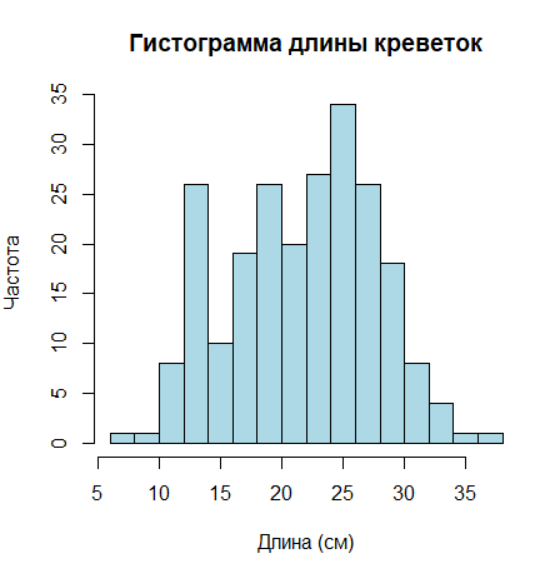
\includegraphics[width=0.6\linewidth,height=\textheight,keepaspectratio]{images/hist_shrimp.PNG}

}

\caption{Рис. 1.1: Гистограмма длины креветок}

\end{figure}%

\subsection{\texorpdfstring{Визуализация в
\texttt{ggridges}}{Визуализация в ggridges}}\label{ux432ux438ux437ux443ux430ux43bux438ux437ux430ux446ux438ux44f-ux432-ggridges}

Для элегантных и компактных графиков подходит библиотека
\texttt{ggridges}. Построим распределение длины креветки в зависимости
от пола и возраста.

\begin{Shaded}
\begin{Highlighting}[]
\FunctionTok{library}\NormalTok{(ggplot2)}
\FunctionTok{library}\NormalTok{(ggridges)}

\FunctionTok{ggplot}\NormalTok{(data, }\FunctionTok{aes}\NormalTok{(}\AttributeTok{x =}\NormalTok{ length, }
                 \AttributeTok{y =}\NormalTok{ sex, }
                 \AttributeTok{group =}\NormalTok{ sex, }
                 \AttributeTok{fill =}\NormalTok{ sex)) }\SpecialCharTok{+}
  \FunctionTok{geom\_density\_ridges}\NormalTok{(}\AttributeTok{scale =} \DecValTok{2}\NormalTok{, }\AttributeTok{alpha =} \FloatTok{0.7}\NormalTok{) }\SpecialCharTok{+}
  \FunctionTok{scale\_y\_discrete}\NormalTok{(}\AttributeTok{expand =} \FunctionTok{c}\NormalTok{(}\DecValTok{0}\NormalTok{, }\DecValTok{0}\NormalTok{)) }\SpecialCharTok{+}
  \FunctionTok{scale\_x\_continuous}\NormalTok{(}\AttributeTok{expand =} \FunctionTok{c}\NormalTok{(}\DecValTok{0}\NormalTok{, }\DecValTok{0}\NormalTok{)) }\SpecialCharTok{+}
  \FunctionTok{labs}\NormalTok{(}
    \AttributeTok{title =} \StringTok{"Распределение длины карапакса по полу"}\NormalTok{,}
    \AttributeTok{x =} \StringTok{"Длина карапакса (мм)"}\NormalTok{,}
    \AttributeTok{y =} \StringTok{"Пол"}
\NormalTok{  ) }\SpecialCharTok{+}
  \FunctionTok{theme}\NormalTok{(}
    \AttributeTok{panel.border =} \FunctionTok{element\_blank}\NormalTok{(),  }\CommentTok{\# Убирает рамку вокруг графика}
    \AttributeTok{axis.line =} \FunctionTok{element\_line}\NormalTok{(}\AttributeTok{color =} \StringTok{"black"}\NormalTok{)  }\CommentTok{\# Сохраняет осевые линии (опционально)}
\NormalTok{  )}
\end{Highlighting}
\end{Shaded}

\begin{figure}[H]

{\centering 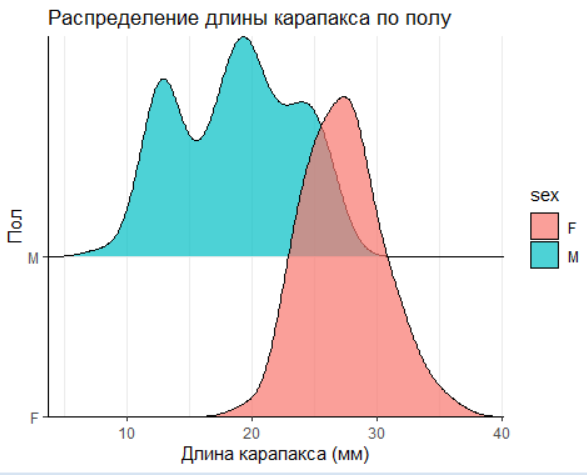
\includegraphics[width=0.6\linewidth,height=\textheight,keepaspectratio]{images/ggridges_shrimp.PNG}

}

\caption{Рис. 1.2: Пол-длина креветок с использованием
\texttt{ggridges}}

\end{figure}%

\section{Выявление аутлайеров
(выбросов)}\label{ux432ux44bux44fux432ux43bux435ux43dux438ux435-ux430ux443ux442ux43bux430ux439ux435ux440ux43eux432-ux432ux44bux431ux440ux43eux441ux43eux432}

Аутлаеры (выбросы) --- наблюдения, значительно отклоняющиеся от общего
распределения данных. Их идентификация критически важна, так как они
могут искажать результаты анализа. Один из надёжных методов обнаружения
выбросов --- \textbf{метод межквартильного размаха (IQR)}.

\subsection{\texorpdfstring{\textbf{Теория
метода}}{Теория метода}}\label{ux442ux435ux43eux440ux438ux44f-ux43cux435ux442ux43eux434ux430}

\begin{enumerate}
\def\labelenumi{\arabic{enumi}.}
\item
  \textbf{Расчёт квартилей}:

  \begin{itemize}
  \item
    \textbf{Q1} (25-й перцентиль): значение, ниже которого находится
    25\% данных.
  \item
    \textbf{Q3} (75-й перцентиль): значение, ниже которого находится
    75\% данных.
  \item
    \textbf{IQR = Q3 - Q1}: мера разброса средней половины данных.
  \end{itemize}
\item
  \textbf{Границы аутлаеров}:

  \begin{itemize}
  \item
    \textbf{Нижняя граница}: Q1−1.5×IQRQ1−1.5×IQR
  \item
    \textbf{Верхняя граница}: Q3+1.5×IQRQ3+1.5×IQR\\
    Наблюдения за этими пределами считаются выбросами.
  \end{itemize}
\end{enumerate}

\subsection{\texorpdfstring{\textbf{Преимущества
метода}}{Преимущества метода}}\label{ux43fux440ux435ux438ux43cux443ux449ux435ux441ux442ux432ux430-ux43cux435ux442ux43eux434ux430}

\begin{itemize}
\item
  Устойчивость к асимметрии распределения.
\item
  Не требует предположения о нормальности данных.
\end{itemize}

\begin{Shaded}
\begin{Highlighting}[]
\CommentTok{\# Метод межквартильного размаха}
\NormalTok{outliers }\OtherTok{\textless{}{-}}\NormalTok{ data }\SpecialCharTok{\%\textgreater{}\%}
  \FunctionTok{mutate}\NormalTok{(}
    \AttributeTok{length\_z =} \FunctionTok{scale}\NormalTok{(length),}
    \AttributeTok{weight\_z =} \FunctionTok{scale}\NormalTok{(weight)}
\NormalTok{  ) }\SpecialCharTok{\%\textgreater{}\%} 
  \FunctionTok{filter}\NormalTok{(}\FunctionTok{abs}\NormalTok{(length\_z) }\SpecialCharTok{\textgreater{}} \DecValTok{3} \SpecialCharTok{|} \FunctionTok{abs}\NormalTok{(weight\_z) }\SpecialCharTok{\textgreater{}} \DecValTok{3}\NormalTok{)}

\CommentTok{\# Визуализация}
\FunctionTok{ggplot}\NormalTok{(data, }\FunctionTok{aes}\NormalTok{(}\AttributeTok{x =}\NormalTok{ length, }\AttributeTok{y =}\NormalTok{ weight)) }\SpecialCharTok{+}
  \FunctionTok{geom\_point}\NormalTok{(}\FunctionTok{aes}\NormalTok{(}\AttributeTok{color =} \StringTok{"Обычные"}\NormalTok{), }\AttributeTok{alpha =} \FloatTok{0.5}\NormalTok{) }\SpecialCharTok{+}
  \FunctionTok{geom\_point}\NormalTok{(}\AttributeTok{data =}\NormalTok{ outliers, }\FunctionTok{aes}\NormalTok{(}\AttributeTok{color =} \StringTok{"Аутлаеры"}\NormalTok{), }\AttributeTok{size =} \DecValTok{3}\NormalTok{) }\SpecialCharTok{+}
  \FunctionTok{scale\_color\_manual}\NormalTok{(}\AttributeTok{values =} \FunctionTok{c}\NormalTok{(}\StringTok{"Обычные"} \OtherTok{=} \StringTok{"grey50"}\NormalTok{, }\StringTok{"Аутлаеры"} \OtherTok{=} \StringTok{"red"}\NormalTok{)) }\SpecialCharTok{+}
  \FunctionTok{labs}\NormalTok{(}\AttributeTok{title =} \StringTok{"Выявление аномальных наблюдений"}\NormalTok{, }\AttributeTok{color =} \StringTok{"Тип"}\NormalTok{)}
\end{Highlighting}
\end{Shaded}

\begin{figure}[H]

{\centering 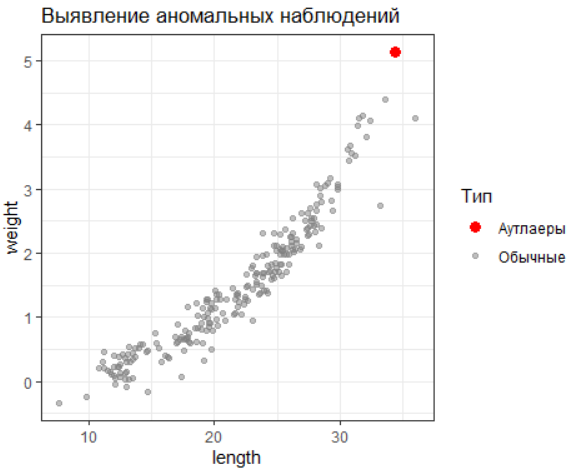
\includegraphics[width=0.6\linewidth,height=\textheight,keepaspectratio]{images/outliers_shrimp.PNG}

}

\caption{Рис. 1.3: Распределение длины карапакса}

\end{figure}%

\section{Определение возрастной структуры: статистические методы анализа
размерных
данных}\label{ux43eux43fux440ux435ux434ux435ux43bux435ux43dux438ux435-ux432ux43eux437ux440ux430ux441ux442ux43dux43eux439-ux441ux442ux440ux443ux43aux442ux443ux440ux44b-ux441ux442ux430ux442ux438ux441ux442ux438ux447ux435ux441ux43aux438ux435-ux43cux435ux442ux43eux434ux44b-ux430ux43dux430ux43bux438ux437ux430-ux440ux430ux437ux43cux435ux440ux43dux44bux445-ux434ux430ux43dux43dux44bux445}

Возрастная структура популяции --- часто важна для расчёта промысловой
смертности, оценки репродуктивного потенциала и прогнозирования динамики
запасов. Поскольку прямое измерение возраста часто невозможно (например,
у беспозвоночных или рыб без четких возрастных меток), используются
статистические методы, выделяющие группы в смешанных распределениях
размеров.

\textbf{Основные подходы:}

\begin{enumerate}
\def\labelenumi{\arabic{enumi}.}
\item
  \textbf{Метод k-средних (k-means)} --- алгоритм кластеризации,
  группирующий особи в заданное число кластеров (возрастных групп) на
  основе их размеров.
\item
  \textbf{Метод Бхаттачарии} --- статистический подход для разделения
  смешанных нормальных распределений, часто применяемый для
  идентификации мод в гистограммах.
\item
  \textbf{EM-алгоритм} --- оценка параметров смеси распределений,
  подходящая для данных с перекрывающимися возрастными группами.
\item
  \textbf{Гауссовы смеси (GMM)} --- расширение метода Бхаттачарии для
  многомерного анализа.
\item
  \textbf{Ядерное сглаживание} --- непараметрический метод визуализации
  плотности, помогающий выявить скрытые моды.
\end{enumerate}

Рассмотрим метод k-средних (k-means) и метод Бхаттачарии, предварительно
построив гистограмму.

\begin{Shaded}
\begin{Highlighting}[]
\CommentTok{\# Загрузка библиотек}
\FunctionTok{library}\NormalTok{(tidyverse)}
\FunctionTok{library}\NormalTok{(mixtools)}
\CommentTok{\# Гистограмма длины с наложением плотности}
\FunctionTok{ggplot}\NormalTok{(data, }\FunctionTok{aes}\NormalTok{(}\AttributeTok{x =}\NormalTok{ length)) }\SpecialCharTok{+}
  \FunctionTok{geom\_histogram}\NormalTok{(}\FunctionTok{aes}\NormalTok{(}\AttributeTok{y =} \FunctionTok{after\_stat}\NormalTok{(density)), }\AttributeTok{fill =} \StringTok{"steelblue"}\NormalTok{, }\AttributeTok{bins =} \DecValTok{20}\NormalTok{, }\AttributeTok{alpha =} \FloatTok{0.7}\NormalTok{) }\SpecialCharTok{+}
  \FunctionTok{geom\_density}\NormalTok{(}\AttributeTok{color =} \StringTok{"\#FC4E07"}\NormalTok{, }\AttributeTok{linewidth =} \DecValTok{1}\NormalTok{) }\SpecialCharTok{+}
  \FunctionTok{labs}\NormalTok{(}\AttributeTok{title =} \StringTok{"Распределение длины карапакса"}\NormalTok{, }
       \AttributeTok{subtitle =} \StringTok{"Пики могут соответствовать возрастным группам"}\NormalTok{,}
       \AttributeTok{x =} \StringTok{"Длина (мм)"}\NormalTok{)}
\end{Highlighting}
\end{Shaded}

\begin{figure}[H]

{\centering 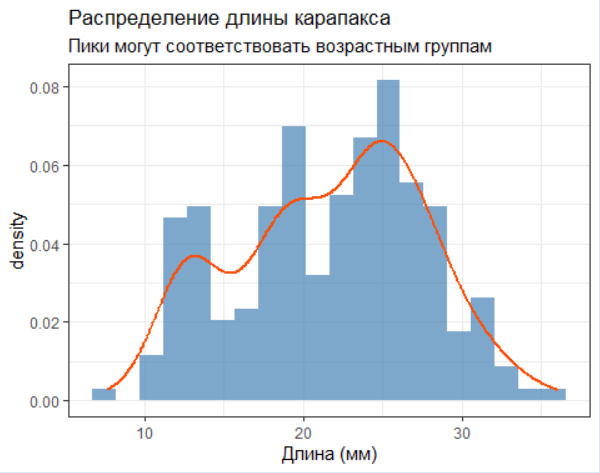
\includegraphics[width=0.6\linewidth,height=\textheight,keepaspectratio]{images/hist_dens_shrimp.PNG}

}

\caption{Рис. 1.3: Распределение длины карапакса}

\end{figure}%

\begin{Shaded}
\begin{Highlighting}[]
\CommentTok{\# Кластеризация по длине (K{-}means как пример)}
\FunctionTok{set.seed}\NormalTok{(}\DecValTok{123}\NormalTok{)}
\NormalTok{clusters }\OtherTok{\textless{}{-}} \FunctionTok{kmeans}\NormalTok{(data}\SpecialCharTok{$}\NormalTok{length, }\AttributeTok{centers =} \DecValTok{4}\NormalTok{)  }\CommentTok{\# Предполагаем 4 возрастные группы}
\NormalTok{data}\SpecialCharTok{$}\NormalTok{cluster }\OtherTok{\textless{}{-}} \FunctionTok{factor}\NormalTok{(clusters}\SpecialCharTok{$}\NormalTok{cluster)}

\CommentTok{\# Визуализация кластеров}
\FunctionTok{ggplot}\NormalTok{(data, }\FunctionTok{aes}\NormalTok{(}\AttributeTok{x =}\NormalTok{ length, }\AttributeTok{fill =}\NormalTok{ cluster)) }\SpecialCharTok{+}
  \FunctionTok{geom\_histogram}\NormalTok{(}\AttributeTok{bins =} \DecValTok{25}\NormalTok{, }\AttributeTok{alpha =} \FloatTok{0.7}\NormalTok{) }\SpecialCharTok{+}
  \FunctionTok{labs}\NormalTok{(}\AttributeTok{title =} \StringTok{"Кластеризация по длине)"}\NormalTok{, }
       \AttributeTok{x =} \StringTok{"Длина (мм)"}\NormalTok{)}
\end{Highlighting}
\end{Shaded}

\begin{figure}[H]

{\centering 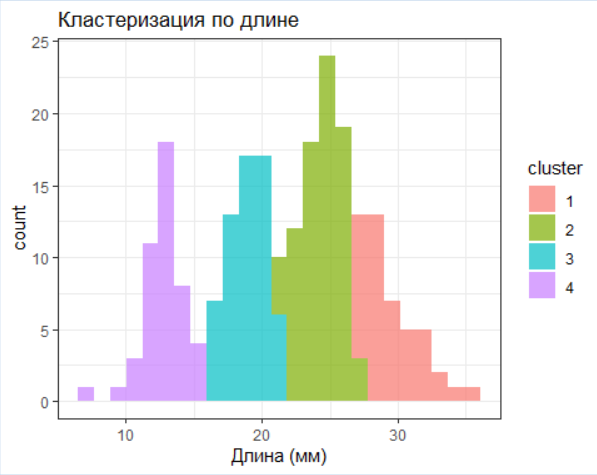
\includegraphics[width=0.6\linewidth,height=\textheight,keepaspectratio]{images/cluster_shrimp.PNG}

}

\caption{Рис. 1.4: Кластеризация по длине}

\end{figure}%

\begin{Shaded}
\begin{Highlighting}[]
\CommentTok{\# Установка рабочей директории}
\FunctionTok{setwd}\NormalTok{(}\StringTok{"C:/TEXTBOOK/"}\NormalTok{)}

\CommentTok{\# Загрузка библиотек}
\FunctionTok{library}\NormalTok{(tidyverse)}
\FunctionTok{library}\NormalTok{(mixtools)}

\CommentTok{\# Загрузка данных}
\NormalTok{data }\OtherTok{\textless{}{-}} \FunctionTok{read.csv}\NormalTok{(}\StringTok{"shrimp\_catch.csv"}\NormalTok{)}

\CommentTok{\# 1. Построение и отображение гистограммы}
\FunctionTok{hist}\NormalTok{(data}\SpecialCharTok{$}\NormalTok{length, }\AttributeTok{breaks =} \DecValTok{20}\NormalTok{, }\AttributeTok{main =} \StringTok{"Гистограмма распределения длин карапаксов"}\NormalTok{,}
     \AttributeTok{xlab =} \StringTok{"Длина карапакса (мм)"}\NormalTok{, }\AttributeTok{ylab =} \StringTok{"Частота"}\NormalTok{)}

\CommentTok{\# 2. Инициализация параметров (предположим 4 возрастные группы)}
\NormalTok{init\_params }\OtherTok{\textless{}{-}} \FunctionTok{list}\NormalTok{(}
  \AttributeTok{lambda =} \FunctionTok{rep}\NormalTok{(}\DecValTok{1}\SpecialCharTok{/}\DecValTok{4}\NormalTok{, }\DecValTok{4}\NormalTok{),}
  \AttributeTok{mu =} \FunctionTok{c}\NormalTok{(}\DecValTok{13}\NormalTok{, }\DecValTok{19}\NormalTok{, }\DecValTok{25}\NormalTok{, }\DecValTok{32}\NormalTok{),}
  \AttributeTok{sigma =} \FunctionTok{c}\NormalTok{(}\FloatTok{1.5}\NormalTok{, }\FloatTok{1.75}\NormalTok{, }\FloatTok{1.75}\NormalTok{, }\FloatTok{2.5}\NormalTok{)}
\NormalTok{)}

\CommentTok{\# 3. Разделение смеси распределений методом EM}
\NormalTok{fit }\OtherTok{\textless{}{-}} \FunctionTok{normalmixEM}\NormalTok{(data}\SpecialCharTok{$}\NormalTok{length, }\AttributeTok{k =} \DecValTok{4}\NormalTok{, }\AttributeTok{maxit =} \DecValTok{1000}\NormalTok{, }\AttributeTok{epsilon =} \FloatTok{1e{-}3}\NormalTok{,}
                   \AttributeTok{lambda =}\NormalTok{ init\_params}\SpecialCharTok{$}\NormalTok{lambda,}
                   \AttributeTok{mu =}\NormalTok{ init\_params}\SpecialCharTok{$}\NormalTok{mu,}
                   \AttributeTok{sigma =}\NormalTok{ init\_params}\SpecialCharTok{$}\NormalTok{sigma)}

\CommentTok{\# 4. Визуализация результатов с ggplot2}
\CommentTok{\# Генерация сетки для построения кривых}
\NormalTok{x\_grid }\OtherTok{\textless{}{-}} \FunctionTok{seq}\NormalTok{(}\FunctionTok{min}\NormalTok{(data}\SpecialCharTok{$}\NormalTok{length), }\FunctionTok{max}\NormalTok{(data}\SpecialCharTok{$}\NormalTok{length), }\AttributeTok{length.out =} \DecValTok{500}\NormalTok{)}

\CommentTok{\# Функция смеси}
\NormalTok{mixture\_density }\OtherTok{\textless{}{-}} \ControlFlowTok{function}\NormalTok{(x) \{}
\NormalTok{  fit}\SpecialCharTok{$}\NormalTok{lambda[}\DecValTok{1}\NormalTok{] }\SpecialCharTok{*} \FunctionTok{dnorm}\NormalTok{(x, fit}\SpecialCharTok{$}\NormalTok{mu[}\DecValTok{1}\NormalTok{], fit}\SpecialCharTok{$}\NormalTok{sigma[}\DecValTok{1}\NormalTok{]) }\SpecialCharTok{+}
\NormalTok{  fit}\SpecialCharTok{$}\NormalTok{lambda[}\DecValTok{2}\NormalTok{] }\SpecialCharTok{*} \FunctionTok{dnorm}\NormalTok{(x, fit}\SpecialCharTok{$}\NormalTok{mu[}\DecValTok{2}\NormalTok{], fit}\SpecialCharTok{$}\NormalTok{sigma[}\DecValTok{2}\NormalTok{]) }\SpecialCharTok{+}
\NormalTok{  fit}\SpecialCharTok{$}\NormalTok{lambda[}\DecValTok{3}\NormalTok{] }\SpecialCharTok{*} \FunctionTok{dnorm}\NormalTok{(x, fit}\SpecialCharTok{$}\NormalTok{mu[}\DecValTok{3}\NormalTok{], fit}\SpecialCharTok{$}\NormalTok{sigma[}\DecValTok{3}\NormalTok{]) }\SpecialCharTok{+}
\NormalTok{  fit}\SpecialCharTok{$}\NormalTok{lambda[}\DecValTok{4}\NormalTok{] }\SpecialCharTok{*} \FunctionTok{dnorm}\NormalTok{(x, fit}\SpecialCharTok{$}\NormalTok{mu[}\DecValTok{4}\NormalTok{], fit}\SpecialCharTok{$}\NormalTok{sigma[}\DecValTok{4}\NormalTok{])}
\NormalTok{\}}

\CommentTok{\# График}
\FunctionTok{ggplot}\NormalTok{(data, }\FunctionTok{aes}\NormalTok{(}\AttributeTok{x =}\NormalTok{ length)) }\SpecialCharTok{+}
  \CommentTok{\# Гистограмма}
  \FunctionTok{geom\_histogram}\NormalTok{(}\FunctionTok{aes}\NormalTok{(}\AttributeTok{y =} \FunctionTok{after\_stat}\NormalTok{(density)), }\AttributeTok{bins =} \DecValTok{20}\NormalTok{, }\AttributeTok{fill =} \StringTok{"white"}\NormalTok{, }\AttributeTok{color =} \StringTok{"black"}\NormalTok{, }\AttributeTok{alpha =} \FloatTok{0.7}\NormalTok{) }\SpecialCharTok{+}
  \CommentTok{\# Исходное распределение (гладкая линия)}
  \FunctionTok{geom\_density}\NormalTok{(}\AttributeTok{color =} \StringTok{"red"}\NormalTok{, }\AttributeTok{lwd =} \FloatTok{1.2}\NormalTok{) }\SpecialCharTok{+}
  \CommentTok{\# Смесь распределений}
  \FunctionTok{stat\_function}\NormalTok{(}\AttributeTok{fun =}\NormalTok{ mixture\_density, }\AttributeTok{color =} \StringTok{"black"}\NormalTok{, }\AttributeTok{lwd =} \FloatTok{1.5}\NormalTok{) }\SpecialCharTok{+}
  \CommentTok{\# Компоненты смеси}
  \FunctionTok{stat\_function}\NormalTok{(}\AttributeTok{fun =} \ControlFlowTok{function}\NormalTok{(x) fit}\SpecialCharTok{$}\NormalTok{lambda[}\DecValTok{1}\NormalTok{] }\SpecialCharTok{*} \FunctionTok{dnorm}\NormalTok{(x, fit}\SpecialCharTok{$}\NormalTok{mu[}\DecValTok{1}\NormalTok{], fit}\SpecialCharTok{$}\NormalTok{sigma[}\DecValTok{1}\NormalTok{]), }\AttributeTok{color =} \StringTok{"blue"}\NormalTok{, }\AttributeTok{lwd =} \DecValTok{1}\NormalTok{) }\SpecialCharTok{+}
  \FunctionTok{stat\_function}\NormalTok{(}\AttributeTok{fun =} \ControlFlowTok{function}\NormalTok{(x) fit}\SpecialCharTok{$}\NormalTok{lambda[}\DecValTok{2}\NormalTok{] }\SpecialCharTok{*} \FunctionTok{dnorm}\NormalTok{(x, fit}\SpecialCharTok{$}\NormalTok{mu[}\DecValTok{2}\NormalTok{], fit}\SpecialCharTok{$}\NormalTok{sigma[}\DecValTok{2}\NormalTok{]), }\AttributeTok{color =} \StringTok{"green"}\NormalTok{, }\AttributeTok{lwd =} \DecValTok{1}\NormalTok{) }\SpecialCharTok{+}
  \FunctionTok{stat\_function}\NormalTok{(}\AttributeTok{fun =} \ControlFlowTok{function}\NormalTok{(x) fit}\SpecialCharTok{$}\NormalTok{lambda[}\DecValTok{3}\NormalTok{] }\SpecialCharTok{*} \FunctionTok{dnorm}\NormalTok{(x, fit}\SpecialCharTok{$}\NormalTok{mu[}\DecValTok{3}\NormalTok{], fit}\SpecialCharTok{$}\NormalTok{sigma[}\DecValTok{3}\NormalTok{]), }\AttributeTok{color =} \StringTok{"orange"}\NormalTok{, }\AttributeTok{lwd =} \DecValTok{1}\NormalTok{) }\SpecialCharTok{+}
  \FunctionTok{stat\_function}\NormalTok{(}\AttributeTok{fun =} \ControlFlowTok{function}\NormalTok{(x) fit}\SpecialCharTok{$}\NormalTok{lambda[}\DecValTok{4}\NormalTok{] }\SpecialCharTok{*} \FunctionTok{dnorm}\NormalTok{(x, fit}\SpecialCharTok{$}\NormalTok{mu[}\DecValTok{4}\NormalTok{], fit}\SpecialCharTok{$}\NormalTok{sigma[}\DecValTok{4}\NormalTok{]), }\AttributeTok{color =} \StringTok{"purple"}\NormalTok{, }\AttributeTok{lwd =} \DecValTok{1}\NormalTok{) }\SpecialCharTok{+}
  
  \CommentTok{\# Настройка темы и легенды}
  \FunctionTok{theme\_minimal}\NormalTok{() }\SpecialCharTok{+}
  \FunctionTok{labs}\NormalTok{(}
    \AttributeTok{x =} \StringTok{"Длина карапакса (мм)"}\NormalTok{,}
    \AttributeTok{y =} \StringTok{"Плотность"}\NormalTok{,}
    \AttributeTok{title =} \StringTok{"Разделение возрастных групп методом EM"}
\NormalTok{  )}
\end{Highlighting}
\end{Shaded}

\begin{figure}[H]

{\centering 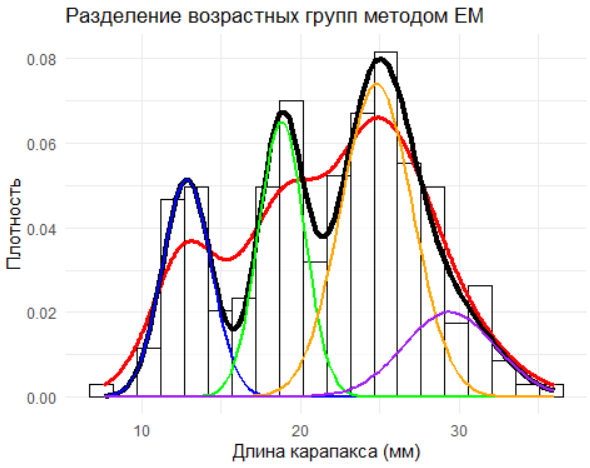
\includegraphics[width=0.6\linewidth,height=\textheight,keepaspectratio]{images/bhattacharya_shrimp.PNG}

}

\caption{Рис. 1.5: Метод Бхаттачарии}

\end{figure}%

\section{Уравнение
Берталанфи}\label{ux443ux440ux430ux432ux43dux435ux43dux438ux435-ux431ux435ux440ux442ux430ux43bux430ux43dux444ux438}

Уравнение Берталанфи --- фундаментальная модель в рыбохозяйственной
науке, описывающая асимптотический рост организмов. Оно имеет вид: \[
L(t) = L_{\infty} \cdot \left(1 - e^{-k \cdot (t - t_0)}\right)
\] где \emph{L\textsubscript{∞}}--- теоретическая максимальная длина
особи, \emph{k}--- коэффициент скорости роста,
\emph{t\textsubscript{0}}--- гипотетический возраст при нулевой длине.

В приведённом коде модель применяется для анализа роста северной
креветки :

\begin{enumerate}
\def\labelenumi{\arabic{enumi}.}
\item
  \textbf{Подготовка данных}: Удаление аутлаеров (например, строк 10 и
  50) повышает точность оценки параметров.
\item
  \textbf{Инициализация параметров}:

  \begin{itemize}
  \item
    \emph{L\textsubscript{∞}} задаётся как максимальная наблюдаемая
    длина в данных.
  \item
    \emph{k} и \emph{t\textsubscript{0}} подбираются итеративно методом
    нелинейных наименьших квадратов (\textbf{\texttt{nls}}).
  \end{itemize}
\item
  \textbf{Визуализация}: График сопоставляет эмпирические данные (точки)
  с предсказаниями модели (красная линия), демонстрируя, как рост
  замедляется с приближением к \emph{L∞}.
\end{enumerate}

\textbf{Интерпретация параметров}:

\begin{itemize}
\item
  Высокое значение \emph{k} (\textgreater0.3) указывает на быстрый рост
  молоди.
\item
  \emph{t\textsubscript{0}}\textless0 может отражать ранний метаморфоз
  личинок.
\end{itemize}

\begin{Shaded}
\begin{Highlighting}[]
\CommentTok{\# Загрузка библиотек}
\FunctionTok{library}\NormalTok{(ggplot2)}
\FunctionTok{library}\NormalTok{(dplyr)}
\FunctionTok{library}\NormalTok{(nlme)}

\CommentTok{\# Загрузка данных}
\NormalTok{data }\OtherTok{\textless{}{-}} \FunctionTok{read.csv}\NormalTok{(}\StringTok{"shrimp\_catch.csv"}\NormalTok{)}

\CommentTok{\# Преобразование возраста в числовой формат}
\NormalTok{data}\SpecialCharTok{$}\NormalTok{age\_num }\OtherTok{\textless{}{-}} \FunctionTok{as.numeric}\NormalTok{(data}\SpecialCharTok{$}\NormalTok{age)}

\CommentTok{\# Удаление аутлайеров (если необходимо)}
\NormalTok{data\_clean }\OtherTok{\textless{}{-}}\NormalTok{ data }\SpecialCharTok{\%\textgreater{}\%}
  \FunctionTok{filter}\NormalTok{(}\SpecialCharTok{!}\NormalTok{id }\SpecialCharTok{\%in\%} \FunctionTok{c}\NormalTok{(}\DecValTok{10}\NormalTok{, }\DecValTok{50}\NormalTok{))  }\CommentTok{\# Пример удаления строк с аномалиями}

\CommentTok{\# Начальные параметры на основе данных}
\NormalTok{L\_inf\_start }\OtherTok{\textless{}{-}} \FunctionTok{max}\NormalTok{(data\_clean}\SpecialCharTok{$}\NormalTok{length, }\AttributeTok{na.rm =} \ConstantTok{TRUE}\NormalTok{)  }\CommentTok{\# Максимальная длина}
\NormalTok{k\_start }\OtherTok{\textless{}{-}} \FloatTok{0.3}                                        \CommentTok{\# Средняя скорость роста}
\NormalTok{t0\_start }\OtherTok{\textless{}{-}} \SpecialCharTok{{-}}\FloatTok{0.5}                                      \CommentTok{\# Гипотетический возраст}

\CommentTok{\# Подгонка модели с увеличенным числом итераций}
\NormalTok{model }\OtherTok{\textless{}{-}} \FunctionTok{nls}\NormalTok{(}
\NormalTok{  length }\SpecialCharTok{\textasciitilde{}}\NormalTok{ L\_inf }\SpecialCharTok{*}\NormalTok{ (}\DecValTok{1} \SpecialCharTok{{-}} \FunctionTok{exp}\NormalTok{(}\SpecialCharTok{{-}}\NormalTok{k }\SpecialCharTok{*}\NormalTok{ (age\_num }\SpecialCharTok{{-}}\NormalTok{ t0))),}
  \AttributeTok{data =}\NormalTok{ data\_clean,}
  \AttributeTok{start =} \FunctionTok{list}\NormalTok{(}\AttributeTok{L\_inf =}\NormalTok{ L\_inf\_start, }\AttributeTok{k =}\NormalTok{ k\_start, }\AttributeTok{t0 =}\NormalTok{ t0\_start),}
  \AttributeTok{control =} \FunctionTok{nls.control}\NormalTok{(}\AttributeTok{maxiter =} \DecValTok{200}\NormalTok{, }\AttributeTok{warnOnly =} \ConstantTok{TRUE}\NormalTok{)  }\CommentTok{\# Увеличиваем лимит итераций}
\NormalTok{)}

\CommentTok{\# Вывод результатов}
\FunctionTok{summary}\NormalTok{(model)}

\CommentTok{\# Создание последовательности возрастов для предсказания}
\NormalTok{age\_seq }\OtherTok{\textless{}{-}} \FunctionTok{seq}\NormalTok{(}\FunctionTok{min}\NormalTok{(data\_clean}\SpecialCharTok{$}\NormalTok{age\_num), }\FunctionTok{max}\NormalTok{(data\_clean}\SpecialCharTok{$}\NormalTok{age\_num), }\AttributeTok{by =} \FloatTok{0.1}\NormalTok{)}

\CommentTok{\# Предсказание значений длины}
\NormalTok{length\_pred }\OtherTok{\textless{}{-}} \FunctionTok{predict}\NormalTok{(model, }\AttributeTok{newdata =} \FunctionTok{data.frame}\NormalTok{(}\AttributeTok{age\_num =}\NormalTok{ age\_seq))}

\CommentTok{\# Построение графика}
\FunctionTok{ggplot}\NormalTok{(data\_clean, }\FunctionTok{aes}\NormalTok{(}\AttributeTok{x =}\NormalTok{ age\_num, }\AttributeTok{y =}\NormalTok{ length)) }\SpecialCharTok{+}
  \FunctionTok{geom\_point}\NormalTok{(}\FunctionTok{aes}\NormalTok{(}\AttributeTok{color =}\NormalTok{ age), }\AttributeTok{alpha =} \FloatTok{0.7}\NormalTok{) }\SpecialCharTok{+}
  \FunctionTok{geom\_line}\NormalTok{(}\AttributeTok{data =} \FunctionTok{data.frame}\NormalTok{(}\AttributeTok{age\_num =}\NormalTok{ age\_seq, }\AttributeTok{length =}\NormalTok{ length\_pred), }
            \FunctionTok{aes}\NormalTok{(}\AttributeTok{x =}\NormalTok{ age\_num, }\AttributeTok{y =}\NormalTok{ length), }\AttributeTok{color =} \StringTok{"red"}\NormalTok{, }\AttributeTok{linewidth =} \FloatTok{1.2}\NormalTok{) }\SpecialCharTok{+}
  \FunctionTok{labs}\NormalTok{(}
    \AttributeTok{title =} \StringTok{"Рост креветок по уравнению Берталанфи"}\NormalTok{,}
    \AttributeTok{x =} \StringTok{"Возраст (годы)"}\NormalTok{,}
    \AttributeTok{y =} \StringTok{"Длина карапакса (мм)"}\NormalTok{,}
    \AttributeTok{color =} \StringTok{"Возрастная группа"}
\NormalTok{  ) }\SpecialCharTok{+}
  \FunctionTok{theme\_minimal}\NormalTok{()}

\CommentTok{\# Сохранение графика}
\FunctionTok{ggsave}\NormalTok{(}\StringTok{"bertalanffy\_model.png"}\NormalTok{, }\AttributeTok{width =} \DecValTok{8}\NormalTok{, }\AttributeTok{height =} \DecValTok{6}\NormalTok{)}
\end{Highlighting}
\end{Shaded}

\begin{figure}[H]

{\centering 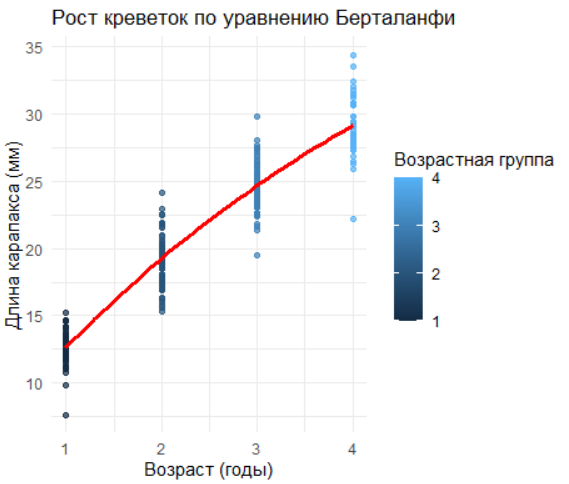
\includegraphics[width=0.6\linewidth,height=\textheight,keepaspectratio]{images/bertalanffy_model.PNG}

}

\caption{Рис. 1.6: Рост креветок по уравнению Берталанфи}

\end{figure}%

\section{Огива, логистическая кривая и 50\%-ное
созревание}\label{ux43eux433ux438ux432ux430-ux43bux43eux433ux438ux441ux442ux438ux447ux435ux441ux43aux430ux44f-ux43aux440ux438ux432ux430ux44f-ux438-50-ux43dux43eux435-ux441ux43eux437ux440ux435ux432ux430ux43dux438ux435}

Логистическая кривая --- ключевой инструмент для моделирования бинарных
процессов, таких как созревание или смена пола у организмов. В случае
протоандрических креветок (\emph{Pandalus borealis}), которые меняют пол
с возрастом, зависимость вероятности быть самкой от длины карапакса
можно описать логистической функцией:

\[
P(F) = \frac{1}{1 + e^{-(\beta_0 + \beta_1 \cdot длина)}}
\]

где \emph{P(F)} --- вероятность принадлежности к женскому полу,
\emph{β\textsubscript{0}} --- интерсепт, \emph{β\textsubscript{1}} ---
коэффициент влияния длины.

Точка перегиба логистической кривой соответствует длине, при которой
вероятность быть самкой равна 50\%: \[
L_{50} = -\frac{\beta_0}{\beta_1}
\]

\begin{figure}[H]

{\centering 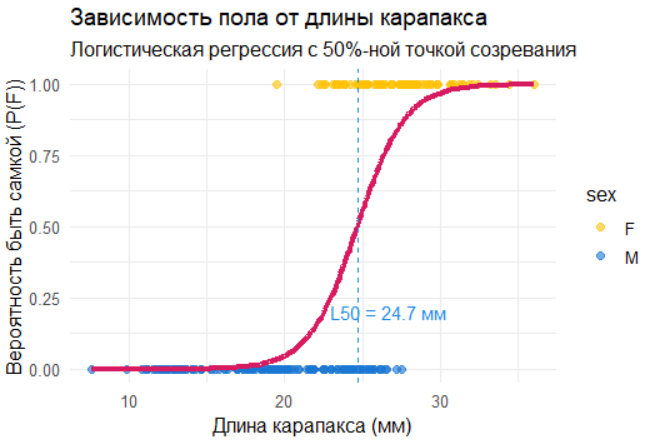
\includegraphics[width=0.6\linewidth,height=\textheight,keepaspectratio]{images/logistic_model_shrimp.PNG}

}

\caption{Рис. 1.7: Логистическая кривая}

\end{figure}%

Огива (кумулятивная кривая) показывает накопление вероятности с
увеличением длины. Для анализа созревания её можно построить через
интеграл логистической функции. Визуально она демонстрирует, как доля
самок возрастает с размером.

\begin{figure}[H]

{\centering 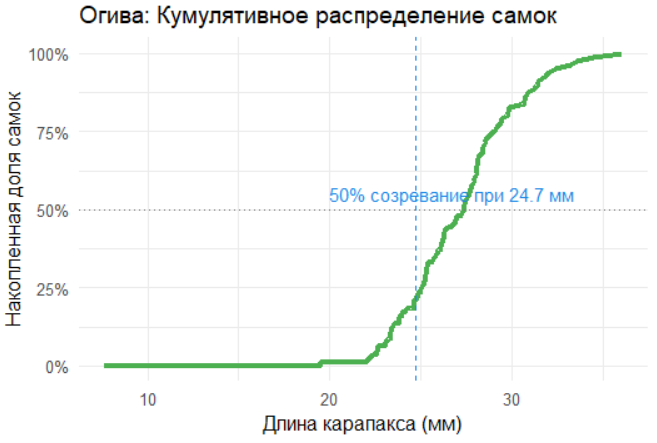
\includegraphics[width=0.6\linewidth,height=\textheight,keepaspectratio]{images/ogive_shrimp.PNG}

}

\caption{Рис. 1.8: Огива}

\end{figure}%

\subsection{\texorpdfstring{\textbf{Оценка
модели}}{Оценка модели}}\label{ux43eux446ux435ux43dux43aux430-ux43cux43eux434ux435ux43bux438}

\begin{enumerate}
\def\labelenumi{\arabic{enumi}.}
\item
  \textbf{ROC-кривая и AUC}:

  \begin{itemize}
  \item
    Площадь под ROC-кривой (AUC) \textgreater0.7 указывает на хорошую
    предсказательную способность модели.
  \item
    Значение AUC = 0.94(пример из кода) подтверждает сильную связь длины
    и пола.
  \end{itemize}
\end{enumerate}

\begin{figure}[H]

{\centering 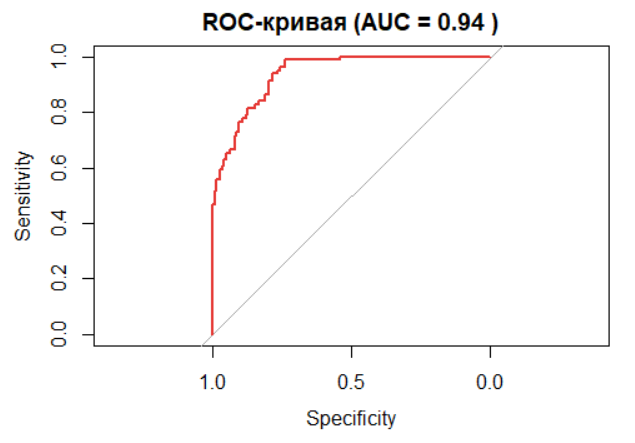
\includegraphics[width=0.6\linewidth,height=\textheight,keepaspectratio]{images/ROC_shrimp.PNG}

}

\caption{Рис. 1.9: ROC-кривая и AUC}

\end{figure}%

\begin{enumerate}
\def\labelenumi{\arabic{enumi}.}
\setcounter{enumi}{1}
\item
  \textbf{Интерпретация коэффициентов}:

  \begin{itemize}
  \item
    Положительный \emph{β\textsubscript{1}} означает: с ростом длины
    вероятность быть самкой увеличивается.
  \item
    Например, \emph{β\textsubscript{1}}=0.25 → увеличение длины на 1 мм
    повышает шансы в e\textsuperscript{0.25}≈1.28 раза.
  \end{itemize}
\end{enumerate}

\subsection{\texorpdfstring{\textbf{Биологический
контекст}}{Биологический контекст}}\label{ux431ux438ux43eux43bux43eux433ux438ux447ux435ux441ux43aux438ux439-ux43aux43eux43dux442ux435ux43aux441ux442}

\begin{itemize}
\item
  \textbf{Протоандрический гермафродитизм}: У креветок смена пола с
  самцов на самок происходит при достижении критического размера
  (\textasciitilde25-28 мм).
\item
  \textbf{L50 как индикатор}: Снижение \emph{L\textsubscript{50}} в
  популяции может сигнализировать о стрессовых условиях (перелов,
  изменение среды), ускоряющих созревание.
\end{itemize}

\begin{Shaded}
\begin{Highlighting}[]
\CommentTok{\# Установка рабочей директории}
\FunctionTok{setwd}\NormalTok{(}\StringTok{"C:/TEXTBOOK/"}\NormalTok{)}

\CommentTok{\# Загрузка библиотек}
\FunctionTok{library}\NormalTok{(tidyverse)}
\FunctionTok{library}\NormalTok{(pROC)}
\FunctionTok{library}\NormalTok{(ggplot2)}

\CommentTok{\# Загрузка данных}
\NormalTok{data }\OtherTok{\textless{}{-}} \FunctionTok{read\_csv}\NormalTok{(}\StringTok{"shrimp\_catch.csv"}\NormalTok{)}

\CommentTok{\# 1. Предобработка данных {-}{-}{-}{-}{-}{-}{-}{-}{-}{-}{-}{-}{-}{-}{-}{-}{-}{-}{-}{-}{-}{-}{-}{-}{-}{-}{-}{-}{-}{-}{-}{-}{-}{-}{-}{-}{-}{-}{-}{-}{-}{-}{-}{-}{-}{-}{-}{-}{-}{-}{-}{-}{-}}
\CommentTok{\# Удаление аутлаеров методом IQR}
\NormalTok{Q1 }\OtherTok{\textless{}{-}} \FunctionTok{quantile}\NormalTok{(data}\SpecialCharTok{$}\NormalTok{length, }\FloatTok{0.25}\NormalTok{)}
\NormalTok{Q3 }\OtherTok{\textless{}{-}} \FunctionTok{quantile}\NormalTok{(data}\SpecialCharTok{$}\NormalTok{length, }\FloatTok{0.75}\NormalTok{)}
\NormalTok{IQR }\OtherTok{\textless{}{-}}\NormalTok{ Q3 }\SpecialCharTok{{-}}\NormalTok{ Q1}
\NormalTok{data\_clean }\OtherTok{\textless{}{-}}\NormalTok{ data }\SpecialCharTok{\%\textgreater{}\%}
  \FunctionTok{filter}\NormalTok{(length }\SpecialCharTok{\textgreater{}=}\NormalTok{ Q1 }\SpecialCharTok{{-}} \FloatTok{1.5}\SpecialCharTok{*}\NormalTok{IQR }\SpecialCharTok{\&}\NormalTok{ length }\SpecialCharTok{\textless{}=}\NormalTok{ Q3 }\SpecialCharTok{+} \FloatTok{1.5}\SpecialCharTok{*}\NormalTok{IQR)}

\CommentTok{\# 2. Логистическая регрессия {-}{-}{-}{-}{-}{-}{-}{-}{-}{-}{-}{-}{-}{-}{-}{-}{-}{-}{-}{-}{-}{-}{-}{-}{-}{-}{-}{-}{-}{-}{-}{-}{-}{-}{-}{-}{-}{-}{-}{-}{-}{-}{-}{-}{-}{-}{-}{-}{-}{-}}
\CommentTok{\# Преобразование пола в бинарную переменную}
\NormalTok{data\_clean}\SpecialCharTok{$}\NormalTok{sex\_binary }\OtherTok{\textless{}{-}} \FunctionTok{ifelse}\NormalTok{(data\_clean}\SpecialCharTok{$}\NormalTok{sex }\SpecialCharTok{==} \StringTok{"F"}\NormalTok{, }\DecValTok{1}\NormalTok{, }\DecValTok{0}\NormalTok{)}

\CommentTok{\# Подгонка модели}
\NormalTok{model\_logit }\OtherTok{\textless{}{-}} \FunctionTok{glm}\NormalTok{(sex\_binary }\SpecialCharTok{\textasciitilde{}}\NormalTok{ length, }
                   \AttributeTok{data =}\NormalTok{ data\_clean, }
                   \AttributeTok{family =} \FunctionTok{binomial}\NormalTok{(}\AttributeTok{link =} \StringTok{"logit"}\NormalTok{))}

\CommentTok{\# Расчет коэффициентов}
\NormalTok{beta0 }\OtherTok{\textless{}{-}} \FunctionTok{coef}\NormalTok{(model\_logit)[}\DecValTok{1}\NormalTok{]}
\NormalTok{beta1 }\OtherTok{\textless{}{-}} \FunctionTok{coef}\NormalTok{(model\_logit)[}\DecValTok{2}\NormalTok{]}

\CommentTok{\# Вычисление L50 (длина 50\% созревания)}
\NormalTok{L50 }\OtherTok{\textless{}{-}} \FunctionTok{round}\NormalTok{(}\SpecialCharTok{{-}}\NormalTok{beta0}\SpecialCharTok{/}\NormalTok{beta1, }\DecValTok{1}\NormalTok{)}

\CommentTok{\# 3. Визуализация {-}{-}{-}{-}{-}{-}{-}{-}{-}{-}{-}{-}{-}{-}{-}{-}{-}{-}{-}{-}{-}{-}{-}{-}{-}{-}{-}{-}{-}{-}{-}{-}{-}{-}{-}{-}{-}{-}{-}{-}{-}{-}{-}{-}{-}{-}{-}{-}{-}{-}{-}{-}{-}{-}{-}{-}{-}{-}{-}{-}}
\CommentTok{\# Логистическая кривая}
\FunctionTok{ggplot}\NormalTok{(data\_clean, }\FunctionTok{aes}\NormalTok{(}\AttributeTok{x =}\NormalTok{ length, }\AttributeTok{y =}\NormalTok{ sex\_binary)) }\SpecialCharTok{+}
  \FunctionTok{geom\_point}\NormalTok{(}\FunctionTok{aes}\NormalTok{(}\AttributeTok{color =}\NormalTok{ sex), }\AttributeTok{alpha =} \FloatTok{0.6}\NormalTok{, }\AttributeTok{size =} \DecValTok{2}\NormalTok{) }\SpecialCharTok{+}
  \FunctionTok{geom\_line}\NormalTok{(}\FunctionTok{aes}\NormalTok{(}\AttributeTok{y =} \FunctionTok{predict}\NormalTok{(model\_logit, }\AttributeTok{type =} \StringTok{"response"}\NormalTok{)), }
            \AttributeTok{color =} \StringTok{"\#D81B60"}\NormalTok{, }\AttributeTok{linewidth =} \FloatTok{1.5}\NormalTok{) }\SpecialCharTok{+}
  \FunctionTok{geom\_vline}\NormalTok{(}\AttributeTok{xintercept =}\NormalTok{ L50, }\AttributeTok{linetype =} \StringTok{"dashed"}\NormalTok{, }\AttributeTok{color =} \StringTok{"\#1E88E5"}\NormalTok{) }\SpecialCharTok{+}
  \FunctionTok{annotate}\NormalTok{(}\StringTok{"text"}\NormalTok{, }\AttributeTok{x =}\NormalTok{ L50 }\SpecialCharTok{+} \DecValTok{2}\NormalTok{, }\AttributeTok{y =} \FloatTok{0.2}\NormalTok{, }
           \AttributeTok{label =} \FunctionTok{paste}\NormalTok{(}\StringTok{"L50 ="}\NormalTok{, L50, }\StringTok{"мм"}\NormalTok{), }\AttributeTok{color =} \StringTok{"\#1E88E5"}\NormalTok{) }\SpecialCharTok{+}
  \FunctionTok{scale\_color\_manual}\NormalTok{(}\AttributeTok{values =} \FunctionTok{c}\NormalTok{(}\StringTok{"\#FFC107"}\NormalTok{, }\StringTok{"\#1976D2"}\NormalTok{)) }\SpecialCharTok{+}
  \FunctionTok{labs}\NormalTok{(}
    \AttributeTok{title =} \StringTok{"Зависимость пола от длины карапакса"}\NormalTok{,}
    \AttributeTok{subtitle =} \StringTok{"Логистическая регрессия с 50\%{-}ной точкой созревания"}\NormalTok{,}
    \AttributeTok{x =} \StringTok{"Длина карапакса (мм)"}\NormalTok{,}
    \AttributeTok{y =} \StringTok{"Вероятность быть самкой (P(F))"}
\NormalTok{  ) }\SpecialCharTok{+}
  \FunctionTok{theme\_minimal}\NormalTok{(}\AttributeTok{base\_size =} \DecValTok{12}\NormalTok{)}

\CommentTok{\# Огива (кумулятивное распределение)}
\NormalTok{data\_ogive }\OtherTok{\textless{}{-}}\NormalTok{ data\_clean }\SpecialCharTok{\%\textgreater{}\%}
  \FunctionTok{arrange}\NormalTok{(length) }\SpecialCharTok{\%\textgreater{}\%}
  \FunctionTok{mutate}\NormalTok{(}
    \AttributeTok{cum\_females =} \FunctionTok{cumsum}\NormalTok{(sex\_binary),}
    \AttributeTok{cum\_prob =}\NormalTok{ cum\_females }\SpecialCharTok{/} \FunctionTok{max}\NormalTok{(cum\_females)}
\NormalTok{  )}

\FunctionTok{ggplot}\NormalTok{(data\_ogive, }\FunctionTok{aes}\NormalTok{(}\AttributeTok{x =}\NormalTok{ length, }\AttributeTok{y =}\NormalTok{ cum\_prob)) }\SpecialCharTok{+}
  \FunctionTok{geom\_line}\NormalTok{(}\AttributeTok{color =} \StringTok{"\#4CAF50"}\NormalTok{, }\AttributeTok{linewidth =} \FloatTok{1.5}\NormalTok{) }\SpecialCharTok{+}
  \FunctionTok{geom\_vline}\NormalTok{(}\AttributeTok{xintercept =}\NormalTok{ L50, }\AttributeTok{linetype =} \StringTok{"dashed"}\NormalTok{, }\AttributeTok{color =} \StringTok{"\#1E88E5"}\NormalTok{) }\SpecialCharTok{+}
  \FunctionTok{geom\_hline}\NormalTok{(}\AttributeTok{yintercept =} \FloatTok{0.5}\NormalTok{, }\AttributeTok{linetype =} \StringTok{"dotted"}\NormalTok{, }\AttributeTok{color =} \StringTok{"\#757575"}\NormalTok{) }\SpecialCharTok{+}
  \FunctionTok{annotate}\NormalTok{(}\StringTok{"text"}\NormalTok{, }\AttributeTok{x =}\NormalTok{ L50 }\SpecialCharTok{+} \DecValTok{2}\NormalTok{, }\AttributeTok{y =} \FloatTok{0.55}\NormalTok{, }
           \AttributeTok{label =} \FunctionTok{paste}\NormalTok{(}\StringTok{"50\% созревание при"}\NormalTok{, L50, }\StringTok{"мм"}\NormalTok{), }\AttributeTok{color =} \StringTok{"\#1E88E5"}\NormalTok{) }\SpecialCharTok{+}
  \FunctionTok{scale\_y\_continuous}\NormalTok{(}\AttributeTok{labels =}\NormalTok{ scales}\SpecialCharTok{::}\NormalTok{percent) }\SpecialCharTok{+}
  \FunctionTok{labs}\NormalTok{(}
    \AttributeTok{title =} \StringTok{"Огива: Кумулятивное распределение самок"}\NormalTok{,}
    \AttributeTok{x =} \StringTok{"Длина карапакса (мм)"}\NormalTok{,}
    \AttributeTok{y =} \StringTok{"Накопленная доля самок"}
\NormalTok{  ) }\SpecialCharTok{+}
  \FunctionTok{theme\_minimal}\NormalTok{(}\AttributeTok{base\_size =} \DecValTok{12}\NormalTok{)}

\CommentTok{\# 4. Оценка модели {-}{-}{-}{-}{-}{-}{-}{-}{-}{-}{-}{-}{-}{-}{-}{-}{-}{-}{-}{-}{-}{-}{-}{-}{-}{-}{-}{-}{-}{-}{-}{-}{-}{-}{-}{-}{-}{-}{-}{-}{-}{-}{-}{-}{-}{-}{-}{-}{-}{-}{-}{-}{-}{-}{-}{-}{-}{-}{-}}
\CommentTok{\# ROC{-}анализ}
\NormalTok{roc\_obj }\OtherTok{\textless{}{-}} \FunctionTok{roc}\NormalTok{(data\_clean}\SpecialCharTok{$}\NormalTok{sex\_binary, }\FunctionTok{predict}\NormalTok{(model\_logit, }\AttributeTok{type =} \StringTok{"response"}\NormalTok{))}
\NormalTok{auc\_value }\OtherTok{\textless{}{-}} \FunctionTok{round}\NormalTok{(}\FunctionTok{auc}\NormalTok{(roc\_obj), }\DecValTok{2}\NormalTok{)}

\CommentTok{\# График ROC{-}кривой}
\FunctionTok{plot}\NormalTok{(roc\_obj, }\AttributeTok{col =} \StringTok{"\#E53935"}\NormalTok{, }\AttributeTok{main =} \FunctionTok{paste}\NormalTok{(}\StringTok{"ROC{-}кривая (AUC ="}\NormalTok{, auc\_value, }\StringTok{")"}\NormalTok{))}

\CommentTok{\# 5. Сохранение результатов {-}{-}{-}{-}{-}{-}{-}{-}{-}{-}{-}{-}{-}{-}{-}{-}{-}{-}{-}{-}{-}{-}{-}{-}{-}{-}{-}{-}{-}{-}{-}{-}{-}{-}{-}{-}{-}{-}{-}{-}{-}{-}{-}{-}{-}{-}{-}{-}{-}{-}}
\FunctionTok{ggsave}\NormalTok{(}\StringTok{"logistic\_curve.png"}\NormalTok{, }\AttributeTok{width =} \DecValTok{8}\NormalTok{, }\AttributeTok{height =} \DecValTok{6}\NormalTok{, }\AttributeTok{dpi =} \DecValTok{300}\NormalTok{)}
\FunctionTok{ggsave}\NormalTok{(}\StringTok{"ogive\_curve.png"}\NormalTok{, }\AttributeTok{width =} \DecValTok{8}\NormalTok{, }\AttributeTok{height =} \DecValTok{6}\NormalTok{, }\AttributeTok{dpi =} \DecValTok{300}\NormalTok{)}

\CommentTok{\# Вывод ключевых метрик}
\FunctionTok{cat}\NormalTok{(}\StringTok{"Результаты анализа:}\SpecialCharTok{\textbackslash{}n}\StringTok{"}\NormalTok{)}
\FunctionTok{cat}\NormalTok{(}\StringTok{"{-} Длина 50\%{-}ного созревания (L50):"}\NormalTok{, L50, }\StringTok{"мм}\SpecialCharTok{\textbackslash{}n}\StringTok{"}\NormalTok{)}
\FunctionTok{cat}\NormalTok{(}\StringTok{"{-} AUC модели:"}\NormalTok{, auc\_value, }\StringTok{"}\SpecialCharTok{\textbackslash{}n}\StringTok{"}\NormalTok{)}
\FunctionTok{cat}\NormalTok{(}\StringTok{"{-} Коэффициенты модели:}\SpecialCharTok{\textbackslash{}n}\StringTok{"}\NormalTok{)}
\FunctionTok{cat}\NormalTok{(}\StringTok{"  Intercept (β0):"}\NormalTok{, }\FunctionTok{round}\NormalTok{(beta0, }\DecValTok{2}\NormalTok{), }\StringTok{"}\SpecialCharTok{\textbackslash{}n}\StringTok{"}\NormalTok{)}
\FunctionTok{cat}\NormalTok{(}\StringTok{"  Slope (β1):"}\NormalTok{, }\FunctionTok{round}\NormalTok{(beta1, }\DecValTok{2}\NormalTok{), }\StringTok{"}\SpecialCharTok{\textbackslash{}n}\StringTok{"}\NormalTok{)}
\end{Highlighting}
\end{Shaded}

\section{Сравнение групп, параметров,
моделей}\label{ux441ux440ux430ux432ux43dux435ux43dux438ux435-ux433ux440ux443ux43fux43f-ux43fux430ux440ux430ux43cux435ux442ux440ux43eux432-ux43cux43eux434ux435ux43bux435ux439}

\subsection{Сравнение групп (на примере самцов и
самок)}\label{ux441ux440ux430ux432ux43dux435ux43dux438ux435-ux433ux440ux443ux43fux43f-ux43dux430-ux43fux440ux438ux43cux435ux440ux435-ux441ux430ux43cux446ux43eux432-ux438-ux441ux430ux43cux43eux43a}

Рассмотрим методы сравнения количественных характеристик (длина, вес)
между самцами и самками северной креветки. Анализ включает проверку
нормальности распределения, выбор подходящего статистического теста и
визуализацию различий.

\subsubsection{Подготовка
данных}\label{ux43fux43eux434ux433ux43eux442ux43eux432ux43aux430-ux434ux430ux43dux43dux44bux445}

Загрузим данные и выделим подвыборки для самцов и самок:

\begin{Shaded}
\begin{Highlighting}[]
\CommentTok{\# Установка рабочей директории}
\FunctionTok{setwd}\NormalTok{(}\StringTok{"C:/TEXTBOOK/"}\NormalTok{)}

\CommentTok{\# Загрузка библиотек  }
\FunctionTok{library}\NormalTok{(tidyverse)  }
\FunctionTok{library}\NormalTok{(ggplot2)  }
\FunctionTok{library}\NormalTok{(rstatix)}
\FunctionTok{library}\NormalTok{(ggpubr)}

\CommentTok{\# Загрузка данных  }
\NormalTok{data }\OtherTok{\textless{}{-}} \FunctionTok{read\_csv}\NormalTok{(}\StringTok{"shrimp\_catch.csv"}\NormalTok{) }\SpecialCharTok{\%\textgreater{}\%}
  \FunctionTok{filter}\NormalTok{(}\SpecialCharTok{!}\NormalTok{id }\SpecialCharTok{\%in\%} \FunctionTok{c}\NormalTok{(}\DecValTok{10}\NormalTok{, }\DecValTok{50}\NormalTok{))  }\CommentTok{\# Удаление аномальных наблюдений }

\CommentTok{\# Фильтрация данных по полу  }
\NormalTok{males }\OtherTok{\textless{}{-}}\NormalTok{ data }\SpecialCharTok{\%\textgreater{}\%} \FunctionTok{filter}\NormalTok{(sex }\SpecialCharTok{==} \StringTok{"M"}\NormalTok{)  }
\NormalTok{females }\OtherTok{\textless{}{-}}\NormalTok{ data }\SpecialCharTok{\%\textgreater{}\%} \FunctionTok{filter}\NormalTok{(sex }\SpecialCharTok{==} \StringTok{"F"}\NormalTok{) }
\end{Highlighting}
\end{Shaded}

\subsubsection{Проверка нормальности
распределения}\label{ux43fux440ux43eux432ux435ux440ux43aux430-ux43dux43eux440ux43cux430ux43bux44cux43dux43eux441ux442ux438-ux440ux430ux441ux43fux440ux435ux434ux435ux43bux435ux43dux438ux44f}

Перед сравнением групп проверим, соответствуют ли данные нормальному
распределению (тест Шапиро-Уилка):

\begin{Shaded}
\begin{Highlighting}[]
\CommentTok{\# Проверка нормальности для длины самцов  }
\FunctionTok{shapiro\_test}\NormalTok{(males}\SpecialCharTok{$}\NormalTok{length)  }
\CommentTok{\# Проверка нормальности для длины самок  }
\FunctionTok{shapiro\_test}\NormalTok{(females}\SpecialCharTok{$}\NormalTok{length) }
\end{Highlighting}
\end{Shaded}

Если p-value \textgreater{} 0.05, распределение считается нормальным. В
противном случае используем непараметрические методы.

\subsubsection{Сравнение средних
значений}\label{ux441ux440ux430ux432ux43dux435ux43dux438ux435-ux441ux440ux435ux434ux43dux438ux445-ux437ux43dux430ux447ux435ux43dux438ux439}

Если данные нормальны: t-тест

\begin{Shaded}
\begin{Highlighting}[]
\CommentTok{\# T{-}тест для сравнения длин самцов и самок  }
\NormalTok{t\_test\_result }\OtherTok{\textless{}{-}} \FunctionTok{t\_test}\NormalTok{(length }\SpecialCharTok{\textasciitilde{}}\NormalTok{ sex, }\AttributeTok{data =}\NormalTok{ data)  }
\NormalTok{t\_test\_result }
\end{Highlighting}
\end{Shaded}

Если данные не нормальны: U-тест Манна-Уитни

\begin{Shaded}
\begin{Highlighting}[]
\CommentTok{\# U{-}тест для сравнения длин самцов и самок  }
\NormalTok{mannwhitney\_result }\OtherTok{\textless{}{-}} \FunctionTok{wilcox\_test}\NormalTok{(length }\SpecialCharTok{\textasciitilde{}}\NormalTok{ sex, }\AttributeTok{data =}\NormalTok{ data)  }
\NormalTok{mannwhitney\_result }
\end{Highlighting}
\end{Shaded}

\subsubsection{Эффект размера (коэффициент
Коэна)}\label{ux44dux444ux444ux435ux43aux442-ux440ux430ux437ux43cux435ux440ux430-ux43aux43eux44dux444ux444ux438ux446ux438ux435ux43dux442-ux43aux43eux44dux43dux430}

Для оценки практической значимости различий рассчитаем коэффициент
Коэна:

\begin{Shaded}
\begin{Highlighting}[]
\CommentTok{\# Расчет коэффициента Коэна  }
\NormalTok{cohens\_d\_result }\OtherTok{\textless{}{-}} \FunctionTok{cohens\_d}\NormalTok{(length }\SpecialCharTok{\textasciitilde{}}\NormalTok{ sex, }\AttributeTok{data =}\NormalTok{ data)  }
\NormalTok{cohens\_d\_result  }
\end{Highlighting}
\end{Shaded}

\begin{itemize}
\item
  \textbf{d \textless{} 0.2} : малый эффект,
\item
  \textbf{d ≈ 0.5} : средний эффект,
\item
  \textbf{d \textgreater{} 0.8} : большой эффект.
\end{itemize}

\subsubsection{\texorpdfstring{\textbf{Визуализация
различий}}{Визуализация различий}}\label{ux432ux438ux437ux443ux430ux43bux438ux437ux430ux446ux438ux44f-ux440ux430ux437ux43bux438ux447ux438ux439}

Построим boxplot для визуального сравнения длин самцов и самок:

\begin{Shaded}
\begin{Highlighting}[]
\FunctionTok{ggplot}\NormalTok{(data, }\FunctionTok{aes}\NormalTok{(}\AttributeTok{x =}\NormalTok{ sex, }\AttributeTok{y =}\NormalTok{ length, }\AttributeTok{fill =}\NormalTok{ sex)) }\SpecialCharTok{+}  
  \FunctionTok{geom\_boxplot}\NormalTok{(}\AttributeTok{color =} \StringTok{"black"}\NormalTok{, }\AttributeTok{alpha =} \FloatTok{0.7}\NormalTok{) }\SpecialCharTok{+}  
  \FunctionTok{stat\_compare\_means}\NormalTok{(}\AttributeTok{method =} \StringTok{"t.test"}\NormalTok{) }\SpecialCharTok{+}  \CommentTok{\# Добавление p{-}value  }
  \FunctionTok{labs}\NormalTok{(}\AttributeTok{title =} \StringTok{"Сравнение длин самцов и самок"}\NormalTok{,  }
       \AttributeTok{x =} \StringTok{"Пол"}\NormalTok{, }\AttributeTok{y =} \StringTok{"Длина карапакса (мм)"}\NormalTok{) }\SpecialCharTok{+}  
  \FunctionTok{theme\_minimal}\NormalTok{() }
\end{Highlighting}
\end{Shaded}

\begin{figure}[H]

{\centering 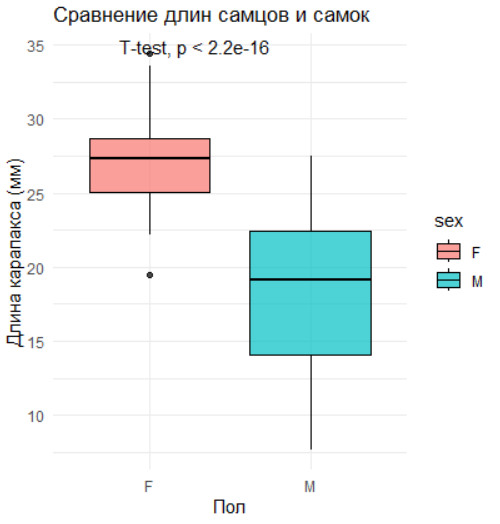
\includegraphics[width=0.6\linewidth,height=\textheight,keepaspectratio]{images/ttest_shrimp.PNG}

}

\caption{Рис. 1.10: Boxplot сравнения длин самцов и самок}

\end{figure}%

\subsubsection{\texorpdfstring{\textbf{Интерпретация
результатов}}{Интерпретация результатов}}\label{ux438ux43dux442ux435ux440ux43fux440ux435ux442ux430ux446ux438ux44f-ux440ux435ux437ux443ux43bux44cux442ux430ux442ux43eux432}

\begin{enumerate}
\def\labelenumi{\arabic{enumi}.}
\item
  Если p-value \textless{} 0.05, различия между группами статистически
  значимы.
\item
  Эффект размера помогает оценить биологическую важность различий.
  Например, если самки значительно крупнее самцов (d = 1.2), это может
  указывать на половой диморфизм, связанный с репродуктивной стратегией.

  \subsubsection{\texorpdfstring{\textbf{Пример полного анализа для
  веса}}{Пример полного анализа для веса}}\label{ux43fux440ux438ux43cux435ux440-ux43fux43eux43bux43dux43eux433ux43e-ux430ux43dux430ux43bux438ux437ux430-ux434ux43bux44f-ux432ux435ux441ux430}
\end{enumerate}

\begin{Shaded}
\begin{Highlighting}[]
\CommentTok{\# Полный анализ для веса  }
\NormalTok{weight\_analysis }\OtherTok{\textless{}{-}}\NormalTok{ data }\SpecialCharTok{\%\textgreater{}\%}  
  \FunctionTok{group\_by}\NormalTok{(sex) }\SpecialCharTok{\%\textgreater{}\%}  
  \FunctionTok{summarise}\NormalTok{(  }
    \AttributeTok{mean\_weight =} \FunctionTok{mean}\NormalTok{(weight),  }
    \AttributeTok{sd\_weight =} \FunctionTok{sd}\NormalTok{(weight),  }
    \AttributeTok{n =} \FunctionTok{n}\NormalTok{()  }
\NormalTok{  ) }\SpecialCharTok{\%\textgreater{}\%}  
  \FunctionTok{mutate}\NormalTok{(  }
    \AttributeTok{t\_test =} \FunctionTok{list}\NormalTok{(}\FunctionTok{t\_test}\NormalTok{(weight }\SpecialCharTok{\textasciitilde{}}\NormalTok{ sex, }\AttributeTok{data =}\NormalTok{ data)),  }
    \AttributeTok{cohens\_d =} \FunctionTok{list}\NormalTok{(}\FunctionTok{cohens\_d}\NormalTok{(weight }\SpecialCharTok{\textasciitilde{}}\NormalTok{ sex, }\AttributeTok{data =}\NormalTok{ data))  }
\NormalTok{  )  }

\CommentTok{\# Вывод результатов  }
\FunctionTok{print}\NormalTok{(weight\_analysis) }

\CommentTok{\# Распределение веса по полу}
\FunctionTok{ggplot}\NormalTok{(data, }\FunctionTok{aes}\NormalTok{(}\AttributeTok{x =} \FunctionTok{factor}\NormalTok{(sex), }\AttributeTok{y =}\NormalTok{ weight, }\AttributeTok{fill =} \FunctionTok{factor}\NormalTok{(sex))) }\SpecialCharTok{+}
  \FunctionTok{geom\_violin}\NormalTok{(}\AttributeTok{trim =} \ConstantTok{FALSE}\NormalTok{, }\AttributeTok{alpha =} \FloatTok{0.7}\NormalTok{) }\SpecialCharTok{+}
  \FunctionTok{geom\_boxplot}\NormalTok{(}\AttributeTok{width =} \FloatTok{0.2}\NormalTok{, }\AttributeTok{outlier.shape =} \ConstantTok{NA}\NormalTok{, }\AttributeTok{fill =} \StringTok{"white"}\NormalTok{) }\SpecialCharTok{+}
  \FunctionTok{labs}\NormalTok{(}\AttributeTok{title =} \StringTok{"Распределение веса по полу"}\NormalTok{, }\AttributeTok{x =} \StringTok{"Пол"}\NormalTok{, }\AttributeTok{y =} \StringTok{"Вес (г)"}\NormalTok{) }\SpecialCharTok{+}
  \FunctionTok{theme\_minimal}\NormalTok{()}
\end{Highlighting}
\end{Shaded}

\begin{figure}[H]

{\centering 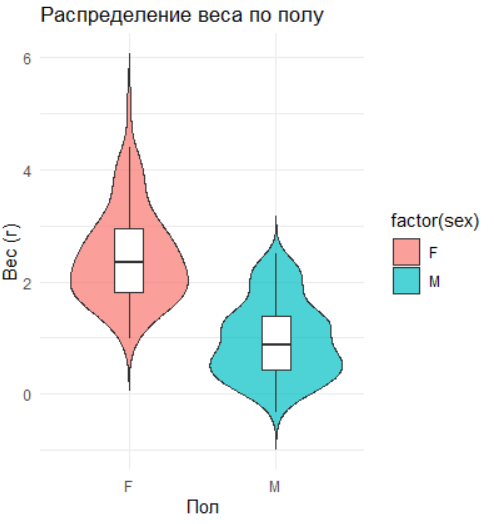
\includegraphics[width=0.6\linewidth,height=\textheight,keepaspectratio]{images/violin_shrimp.PNG}

}

\caption{Рис. 1.12: Violin plot для визуализации распределения веса}

\end{figure}%

\subsubsection{\texorpdfstring{\textbf{Выводы}}{Выводы}}\label{ux432ux44bux432ux43eux434ux44b}

\begin{enumerate}
\def\labelenumi{\arabic{enumi}.}
\item
  Используйте t-тест для нормальных данных и U-тест для ненормальных.
\item
  Дополните анализ оценкой эффекта размера для биологической
  интерпретации.
\item
  Визуализируйте различия с помощью boxplot или violin plot.
\end{enumerate}

\textbf{Рекомендации} :

\begin{itemize}
\item
  Для многомерных данных (например, одновременное сравнение длины, веса
  и возраста) применяйте MANOVA.
\item
  Если группы неоднородны (например, разный возрастной состав),
  используйте ковариационный анализ (ANCOVA).

  \subsection{\texorpdfstring{\textbf{Что делать, если тест на
  нормальность не пройден для одной из
  групп?}}{Что делать, если тест на нормальность не пройден для одной из групп?}}\label{ux447ux442ux43e-ux434ux435ux43bux430ux442ux44c-ux435ux441ux43bux438-ux442ux435ux441ux442-ux43dux430-ux43dux43eux440ux43cux430ux43bux44cux43dux43eux441ux442ux44c-ux43dux435-ux43fux440ux43eux439ux434ux435ux43d-ux434ux43bux44f-ux43eux434ux43dux43eux439-ux438ux437-ux433ux440ux443ux43fux43f}

  При сравнении количественных характеристик (например, длины карапакса
  у самцов и самок) важно учитывать, соответствуют ли данные нормальному
  распределению. Если тест на нормальность (например, Шапиро-Уилка)
  показывает значимое отклонение от нормальности для одной из групп, это
  влияет на выбор статистического теста и интерпретацию результатов.

  \subsubsection{\texorpdfstring{\textbf{Пример из нашего
  анализа}}{Пример из нашего анализа}}\label{ux43fux440ux438ux43cux435ux440-ux438ux437-ux43dux430ux448ux435ux433ux43e-ux430ux43dux430ux43bux438ux437ux430}

  Мы провели сравнение длины карапакса между самцами и самками:

  \begin{itemize}
  \item
    Для самцов: \textbf{\texttt{shapiro\_test(males\$length)}} → p-value
    = \textbf{0.000574} (нормальность отвергнута).
  \item
    Для самок: \textbf{\texttt{shapiro\_test(females\$length)}} →
    p-value = \textbf{0.891} (нормальность подтверждена).
  \end{itemize}

  Несмотря на это, мы применили как \textbf{t-тест} , так и
  \textbf{U-тест Манна-Уитни} :

  \begin{itemize}
  \item
    \textbf{t-тест} : p-value = 1.46e-40 (значимо).
  \item
    \textbf{U-тест} : p-value = 1.97e-27 (значимо).
  \item
    Коэффициент Коэна: d = 2.14 (большой эффект).
  \end{itemize}

  \subsubsection{\texorpdfstring{\textbf{Почему это
  работает?}}{Почему это работает?}}\label{ux43fux43eux447ux435ux43cux443-ux44dux442ux43e-ux440ux430ux431ux43eux442ux430ux435ux442}

  \begin{enumerate}
  \def\labelenumi{\arabic{enumi}.}
  \item
    \textbf{t-тест устойчив к умеренным отклонениям от нормальности} :

    \begin{itemize}
    \item
      При больших выборках (n \textgreater{} 30) центральная предельная
      теорема позволяет использовать t-тест даже при слабо выраженной
      асимметрии.
    \item
      В вашем случае выборка самцов (n = 149) достаточно велика, чтобы
      компенсировать отклонение от нормальности.
    \end{itemize}
  \item
    \textbf{U-тест Манна-Уитни --- непараметрическая альтернатива} :

    \begin{itemize}
    \item
      Этот тест не требует нормальности и сравнивает ранги, а не средние
      значения.
    \item
      Он подтверждает значимость различий, что усиливает доверие к
      выводу.
    \end{itemize}
  \item
    \textbf{Эффект размера (коэффициент Кобена)} :

    \begin{itemize}
    \tightlist
    \item
      d = 2.14 указывает на \textbf{большой эффект} , что важно для
      биологической интерпретации, даже если p-values значимы.
    \end{itemize}
  \end{enumerate}
\end{itemize}

\subsection{Сравнение параметров (линейные модели для оценки
межгрупповых
различий)}\label{ux441ux440ux430ux432ux43dux435ux43dux438ux435-ux43fux430ux440ux430ux43cux435ux442ux440ux43eux432-ux43bux438ux43dux435ux439ux43dux44bux435-ux43cux43eux434ux435ux43bux438-ux434ux43bux44f-ux43eux446ux435ux43dux43aux438-ux43cux435ux436ux433ux440ux443ux43fux43fux43eux432ux44bux445-ux440ux430ux437ux43bux438ux447ux438ux439}

Для сравнения параметров двух линейных моделей (например, скорости роста
самцов и самок) используем следующий подход.

\begin{Shaded}
\begin{Highlighting}[]
\CommentTok{\# Установка рабочей директории}
\FunctionTok{setwd}\NormalTok{(}\StringTok{"C:/TEXTBOOK/"}\NormalTok{)}

\CommentTok{\# Загрузка библиотек}
\FunctionTok{library}\NormalTok{(tidyverse)}
\FunctionTok{library}\NormalTok{(ggplot2)}
\FunctionTok{library}\NormalTok{(broom)}
\FunctionTok{library}\NormalTok{(knitr)}

\CommentTok{\# Загрузка данных}
\NormalTok{data }\OtherTok{\textless{}{-}} \FunctionTok{read\_csv}\NormalTok{(}\StringTok{"shrimp\_catch.csv"}\NormalTok{) }\SpecialCharTok{\%\textgreater{}\%}
  \FunctionTok{filter}\NormalTok{(}\SpecialCharTok{!}\NormalTok{id }\SpecialCharTok{\%in\%} \FunctionTok{c}\NormalTok{(}\DecValTok{10}\NormalTok{, }\DecValTok{50}\NormalTok{))  }\CommentTok{\# Удаление аномальных наблюдений}

\CommentTok{\# Фильтрация данных по полу}
\NormalTok{data\_male }\OtherTok{\textless{}{-}}\NormalTok{ data }\SpecialCharTok{\%\textgreater{}\%} \FunctionTok{filter}\NormalTok{(sex }\SpecialCharTok{==} \StringTok{"M"}\NormalTok{)}
\NormalTok{data\_female }\OtherTok{\textless{}{-}}\NormalTok{ data }\SpecialCharTok{\%\textgreater{}\%} \FunctionTok{filter}\NormalTok{(sex }\SpecialCharTok{==} \StringTok{"F"}\NormalTok{)}

\CommentTok{\# Построение моделей}
\NormalTok{model\_male }\OtherTok{\textless{}{-}} \FunctionTok{lm}\NormalTok{(length }\SpecialCharTok{\textasciitilde{}}\NormalTok{ age, }\AttributeTok{data =}\NormalTok{ data\_male)}
\NormalTok{model\_female }\OtherTok{\textless{}{-}} \FunctionTok{lm}\NormalTok{(length }\SpecialCharTok{\textasciitilde{}}\NormalTok{ age, }\AttributeTok{data =}\NormalTok{ data\_female)}

\FunctionTok{ggplot}\NormalTok{(data, }\FunctionTok{aes}\NormalTok{(age, length, }\AttributeTok{color =}\NormalTok{ sex)) }\SpecialCharTok{+}
  \FunctionTok{geom\_point}\NormalTok{(}\AttributeTok{alpha =} \FloatTok{0.5}\NormalTok{) }\SpecialCharTok{+}
  \FunctionTok{geom\_smooth}\NormalTok{(}\AttributeTok{method =} \StringTok{"lm"}\NormalTok{, }\AttributeTok{formula =}\NormalTok{ y }\SpecialCharTok{\textasciitilde{}}\NormalTok{ x) }\SpecialCharTok{+}
  \FunctionTok{scale\_color\_manual}\NormalTok{(}\AttributeTok{values =} \FunctionTok{c}\NormalTok{(}\StringTok{"\#E7B800"}\NormalTok{, }\StringTok{"\#00AFBB"}\NormalTok{)) }\SpecialCharTok{+}
  \FunctionTok{labs}\NormalTok{(}\AttributeTok{x =} \StringTok{"Возраст"}\NormalTok{, }\AttributeTok{y =} \StringTok{"Длина (мм)"}\NormalTok{) }\SpecialCharTok{+}
  \FunctionTok{theme\_minimal}\NormalTok{()}
\end{Highlighting}
\end{Shaded}

\begin{figure}[H]

{\centering 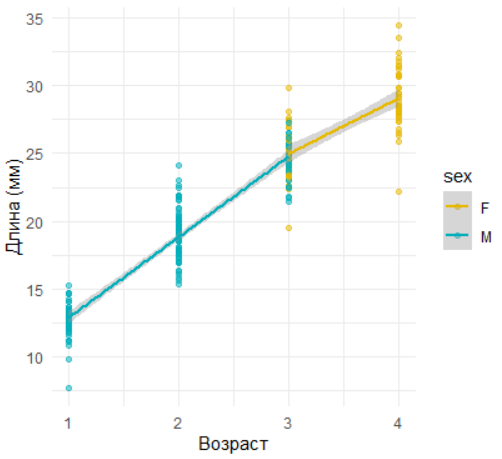
\includegraphics[width=0.6\linewidth,height=\textheight,keepaspectratio]{images/comparison_shrimp.PNG}

}

\caption{Рис. 1.15: Визуализация моделей}

\end{figure}%

\textbf{Метод 1: Объединенная модель с взаимодействиями}

\begin{Shaded}
\begin{Highlighting}[]
\CommentTok{\# Установка рабочей директории}
\NormalTok{joint\_model }\OtherTok{\textless{}{-}} \FunctionTok{lm}\NormalTok{(length }\SpecialCharTok{\textasciitilde{}}\NormalTok{ age }\SpecialCharTok{*}\NormalTok{ sex, }\AttributeTok{data =}\NormalTok{ data)}
\FunctionTok{summary}\NormalTok{(joint\_model) }\SpecialCharTok{\%\textgreater{}\%} 
\NormalTok{  broom}\SpecialCharTok{::}\FunctionTok{tidy}\NormalTok{() }\SpecialCharTok{\%\textgreater{}\%} 
  \FunctionTok{filter}\NormalTok{(term }\SpecialCharTok{==} \StringTok{"age:sexM"}\NormalTok{) }\SpecialCharTok{\%\textgreater{}\%} 
  \FunctionTok{kable}\NormalTok{(}\AttributeTok{caption =} \StringTok{"Проверка различия наклонов"}\NormalTok{, }\AttributeTok{digits =} \DecValTok{3}\NormalTok{)}
\end{Highlighting}
\end{Shaded}

\begin{Shaded}
\begin{Highlighting}[]
\NormalTok{Table}\SpecialCharTok{:}\NormalTok{ Проверка различия наклонов}

\SpecialCharTok{|}\NormalTok{term     }\SpecialCharTok{|}\NormalTok{ estimate}\SpecialCharTok{|}\NormalTok{ std.error}\SpecialCharTok{|}\NormalTok{ statistic}\SpecialCharTok{|}\NormalTok{ p.value}\SpecialCharTok{|}
\ErrorTok{|:}\SpecialCharTok{{-}{-}{-}{-}{-}{-}{-}{-}}\ErrorTok{|}\SpecialCharTok{{-}{-}{-}{-}{-}{-}{-}{-}}\ErrorTok{:|}\SpecialCharTok{{-}{-}{-}{-}{-}{-}{-}{-}{-}}\ErrorTok{:|}\SpecialCharTok{{-}{-}{-}{-}{-}{-}{-}{-}{-}}\ErrorTok{:|}\SpecialCharTok{{-}{-}{-}{-}{-}{-}{-}}\ErrorTok{:|}
\ErrorTok{|}\NormalTok{age}\SpecialCharTok{:}\NormalTok{sexM }\SpecialCharTok{|}     \FloatTok{1.86}\SpecialCharTok{|}     \FloatTok{0.459}\SpecialCharTok{|}     \FloatTok{4.053}\SpecialCharTok{|}       \DecValTok{0}\SpecialCharTok{|}
\ErrorTok{\textgreater{}} 
\end{Highlighting}
\end{Shaded}

\textbf{Интерпретация:}\\
Значимый коэффициент взаимодействия \textbf{\texttt{age:sexM}} (p
\textless{} 0.05) указывает на статистически значимые различия в
скорости роста между полами.

\textbf{Метод 2: Тест Вальда}

\begin{Shaded}
\begin{Highlighting}[]
\FunctionTok{library}\NormalTok{(car)}
\NormalTok{delta\_beta }\OtherTok{\textless{}{-}} \FunctionTok{coef}\NormalTok{(model\_male)[}\StringTok{"age"}\NormalTok{] }\SpecialCharTok{{-}} \FunctionTok{coef}\NormalTok{(model\_female)[}\StringTok{"age"}\NormalTok{]}
\NormalTok{se\_diff }\OtherTok{\textless{}{-}} \FunctionTok{sqrt}\NormalTok{(}\FunctionTok{vcov}\NormalTok{(model\_male)[}\StringTok{"age"}\NormalTok{,}\StringTok{"age"}\NormalTok{] }\SpecialCharTok{+} \FunctionTok{vcov}\NormalTok{(model\_female)[}\StringTok{"age"}\NormalTok{,}\StringTok{"age"}\NormalTok{])}
\NormalTok{z\_score }\OtherTok{\textless{}{-}}\NormalTok{ delta\_beta }\SpecialCharTok{/}\NormalTok{ se\_diff}
\NormalTok{p\_value }\OtherTok{\textless{}{-}} \DecValTok{2} \SpecialCharTok{*} \FunctionTok{pnorm}\NormalTok{(}\SpecialCharTok{{-}}\FunctionTok{abs}\NormalTok{(z\_score))}

\FunctionTok{cat}\NormalTok{(}\StringTok{"Разница коэффициентов:"}\NormalTok{, }\FunctionTok{round}\NormalTok{(delta\_beta, }\DecValTok{3}\NormalTok{), }
    \StringTok{"}\SpecialCharTok{\textbackslash{}n}\StringTok{Z{-}статистика:"}\NormalTok{, }\FunctionTok{round}\NormalTok{(z\_score, }\DecValTok{3}\NormalTok{),}
    \StringTok{"}\SpecialCharTok{\textbackslash{}n}\StringTok{p{-}value:"}\NormalTok{, }\FunctionTok{format.pval}\NormalTok{(p\_value, }\AttributeTok{digits =} \DecValTok{2}\NormalTok{))}


\NormalTok{comparison\_table }\OtherTok{\textless{}{-}} \FunctionTok{data.frame}\NormalTok{(}
\NormalTok{  Параметр }\OtherTok{=} \FunctionTok{c}\NormalTok{(}\StringTok{"Скорость роста самцов"}\NormalTok{, }\StringTok{"Скорость роста самок"}\NormalTok{, }\StringTok{"Разница"}\NormalTok{),}
\NormalTok{  Значение }\OtherTok{=} \FunctionTok{c}\NormalTok{(}
    \FunctionTok{round}\NormalTok{(}\FunctionTok{coef}\NormalTok{(model\_male)[}\StringTok{"age"}\NormalTok{], }\DecValTok{2}\NormalTok{),}
    \FunctionTok{round}\NormalTok{(}\FunctionTok{coef}\NormalTok{(model\_female)[}\StringTok{"age"}\NormalTok{], }\DecValTok{2}\NormalTok{),}
    \FunctionTok{round}\NormalTok{(delta\_beta, }\DecValTok{2}\NormalTok{)}
\NormalTok{  ),}
  \StringTok{\textasciigrave{}}\AttributeTok{p{-}value}\StringTok{\textasciigrave{}} \OtherTok{=} \FunctionTok{c}\NormalTok{(}
    \FunctionTok{format.pval}\NormalTok{(}\FunctionTok{summary}\NormalTok{(model\_male)}\SpecialCharTok{$}\NormalTok{coefficients[}\StringTok{"age"}\NormalTok{,}\DecValTok{4}\NormalTok{], }\AttributeTok{digits =} \DecValTok{2}\NormalTok{),}
    \FunctionTok{format.pval}\NormalTok{(}\FunctionTok{summary}\NormalTok{(model\_female)}\SpecialCharTok{$}\NormalTok{coefficients[}\StringTok{"age"}\NormalTok{,}\DecValTok{4}\NormalTok{], }\AttributeTok{digits =} \DecValTok{2}\NormalTok{),}
    \FunctionTok{format.pval}\NormalTok{(p\_value, }\AttributeTok{digits =} \DecValTok{2}\NormalTok{)}
\NormalTok{  )}
\NormalTok{)}
\FunctionTok{kable}\NormalTok{(comparison\_table, }\AttributeTok{caption =} \StringTok{"Сравнение коэффициентов роста"}\NormalTok{)}
\end{Highlighting}
\end{Shaded}

Вывод

\begin{Shaded}
\begin{Highlighting}[]
\SpecialCharTok{:}\NormalTok{ Сравнение коэффициентов роста}

\SpecialCharTok{|}\NormalTok{Параметр              }\SpecialCharTok{|}\NormalTok{ Значение}\SpecialCharTok{|}\NormalTok{p.value }\SpecialCharTok{|}
\ErrorTok{|:}\SpecialCharTok{{-}{-}{-}{-}{-}{-}{-}{-}{-}{-}{-}{-}{-}{-}{-}{-}{-}{-}{-}{-}{-}}\ErrorTok{|}\SpecialCharTok{{-}{-}{-}{-}{-}{-}{-}{-}}\ErrorTok{:|:}\SpecialCharTok{{-}{-}{-}{-}{-}{-}{-}}\ErrorTok{|}
\ErrorTok{|}\NormalTok{Скорость роста самцов }\SpecialCharTok{|}     \FloatTok{5.95}\SpecialCharTok{|}\ErrorTok{\textless{}}\FloatTok{2e{-}16}  \SpecialCharTok{|}
\ErrorTok{|}\NormalTok{Скорость роста самок  }\SpecialCharTok{|}     \FloatTok{4.09}\SpecialCharTok{|}\FloatTok{5.2e{-}13} \SpecialCharTok{|}
\ErrorTok{|}\NormalTok{Разница               }\SpecialCharTok{|}     \FloatTok{1.86}\SpecialCharTok{|}\FloatTok{0.00024} \SpecialCharTok{|}
\ErrorTok{\textgreater{}} 
\end{Highlighting}
\end{Shaded}

\textbf{Интерпретация:}\\
Значимая \emph{разница} (p \textless{} 0.05) указывает на статистически
значимые различия в скорости роста между полами.

\subsection{Сравнение
моделей}\label{ux441ux440ux430ux432ux43dux435ux43dux438ux435-ux43cux43eux434ux435ux43bux435ux439}

Одним из ключевых аспектов анализа биологических данных является
определение формы зависимости между переменными. В данном разделе мы
рассмотрим основы подбора модели зависимости между длиной и весом
креветок. Начиная с простой линейной модели, мы постепенно перейдем к
более сложным нелинейным моделям, чтобы продемонстрировать методику
выбора наилучшей модели. Cравним три модели --- линейную, полиномиальную
и степенную --- чтобы определить, какая из них наилучшим образом
описывает данные. Цель анализа --- найти математическую зависимость,
которая:

\begin{enumerate}
\def\labelenumi{\arabic{enumi}.}
\item
  Точно предсказывает вес креветки по её длине.
\item
  Имеет биологическую интерпретацию.
\item
  Минимизирует ошибку предсказания.
\end{enumerate}

\subsubsection{Модели и их
параметры}\label{ux43cux43eux434ux435ux43bux438-ux438-ux438ux445-ux43fux430ux440ux430ux43cux435ux442ux440ux44b}

\begin{enumerate}
\def\labelenumi{\arabic{enumi}.}
\tightlist
\item
  \textbf{Линейная}:
  \(\text{weight} = \beta_0 + \beta_1\cdot\text{length}\)
\item
  \textbf{Полиномиальная 3-й степени}:
  \(\text{weight} = \beta_0 + \beta_1\cdot\text{length} + \beta_2\cdot\text{length}^2 + \beta_3\cdot\text{length}^3\)
\item
  \textbf{Степенная}: \(\text{weight} = a\cdot\text{length}^b\)
\end{enumerate}

\subsubsection{Метрики}\label{ux43cux435ux442ux440ux438ux43aux438}

\begin{itemize}
\tightlist
\item
  \textbf{R²} - (коэффициент детерминации): чем ближе к 1, тем лучше
  модель объясняет данные.
\item
  \textbf{AIC} -(информационный критерий Акаике): чем меньше значение,
  тем лучше модель с учётом её сложности.
\end{itemize}

\subsubsection{\texorpdfstring{\textbf{Результаты}}{Результаты}}\label{ux440ux435ux437ux443ux43bux44cux442ux430ux442ux44b}

\paragraph{\texorpdfstring{\textbf{1. Линейная
модель}}{1. Линейная модель}}\label{ux43bux438ux43dux435ux439ux43dux430ux44f-ux43cux43eux434ux435ux43bux44c}

\begin{Shaded}
\begin{Highlighting}[]
\NormalTok{Coefficients}\SpecialCharTok{:}
\NormalTok{             Estimate Std. Error t value }\FunctionTok{Pr}\NormalTok{(}\SpecialCharTok{\textgreater{}}\ErrorTok{|}\NormalTok{t}\SpecialCharTok{|}\NormalTok{)    }
\NormalTok{(Intercept) }\SpecialCharTok{{-}}\FloatTok{2.115}      \FloatTok{0.085}     \SpecialCharTok{{-}}\FloatTok{24.86}   \SpecialCharTok{\textless{}}\FloatTok{2e{-}16} \SpecialCharTok{**}\ErrorTok{*}
\NormalTok{length       }\FloatTok{0.1665}     \FloatTok{0.0038}    \FloatTok{43.71}    \SpecialCharTok{\textless{}}\FloatTok{2e{-}16} \SpecialCharTok{**}\ErrorTok{*}
\end{Highlighting}
\end{Shaded}

\begin{itemize}
\item
  \textbf{R² = 0.894}
\item
  \textbf{AIC = 148.02}
\end{itemize}

\begin{figure}[H]

{\centering 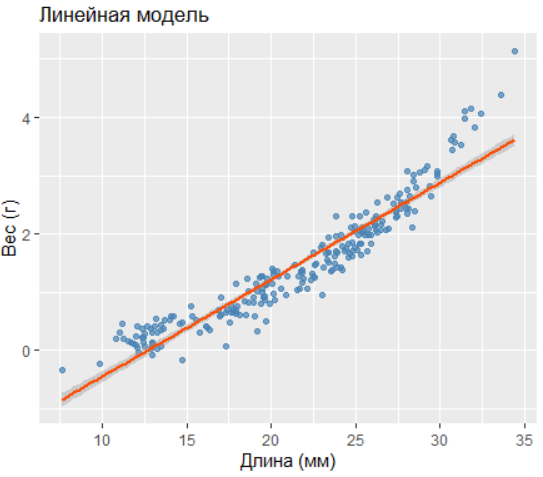
\includegraphics[width=0.6\linewidth,height=\textheight,keepaspectratio]{images/linear_shrimp.PNG}

}

\caption{Рис. 1.5: Линейная модель}

\end{figure}%

\paragraph{\texorpdfstring{\textbf{2. Полиномиальная
модель}}{2. Полиномиальная модель}}\label{ux43fux43eux43bux438ux43dux43eux43cux438ux430ux43bux44cux43dux430ux44f-ux43cux43eux434ux435ux43bux44c}

\begin{Shaded}
\begin{Highlighting}[]
\NormalTok{Coefficients}\SpecialCharTok{:}
\NormalTok{                 Estimate Std. Error t value }\FunctionTok{Pr}\NormalTok{(}\SpecialCharTok{\textgreater{}}\ErrorTok{|}\NormalTok{t}\SpecialCharTok{|}\NormalTok{)    }
\FunctionTok{poly}\NormalTok{(length,}\DecValTok{3}\NormalTok{)}\DecValTok{1}  \FloatTok{14.5038}    \FloatTok{0.2127}    \FloatTok{68.18}   \SpecialCharTok{\textless{}}\FloatTok{2e{-}16} \SpecialCharTok{**}\ErrorTok{*}
\FunctionTok{poly}\NormalTok{(length,}\DecValTok{3}\NormalTok{)}\DecValTok{2}   \FloatTok{3.7209}    \FloatTok{0.2127}    \FloatTok{17.49}   \SpecialCharTok{\textless{}}\FloatTok{2e{-}16} \SpecialCharTok{**}\ErrorTok{*}
\FunctionTok{poly}\NormalTok{(length,}\DecValTok{3}\NormalTok{)}\DecValTok{3}   \FloatTok{0.9526}    \FloatTok{0.2127}     \FloatTok{4.48}  \FloatTok{1.2e{-}05} \SpecialCharTok{**}\ErrorTok{*}
\end{Highlighting}
\end{Shaded}

\begin{itemize}
\item
  \textbf{R² = 0.957}
\item
  \textbf{AIC = -52.80}
\end{itemize}

\begin{figure}[H]

{\centering 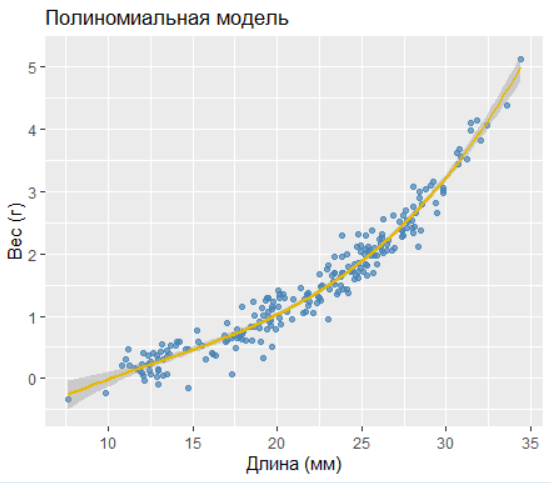
\includegraphics[width=0.6\linewidth,height=\textheight,keepaspectratio]{images/poly_shrimp.PNG}

}

\caption{Рис. 1.5: Полиномиальная модель}

\end{figure}%

\paragraph{\texorpdfstring{\textbf{3. Степенная
модель}}{3. Степенная модель}}\label{ux441ux442ux435ux43fux435ux43dux43dux430ux44f-ux43cux43eux434ux435ux43bux44c}

\begin{Shaded}
\begin{Highlighting}[]
\NormalTok{Parameters}\SpecialCharTok{:}
\NormalTok{   Estimate Std. Error t value }\FunctionTok{Pr}\NormalTok{(}\SpecialCharTok{\textgreater{}}\ErrorTok{|}\NormalTok{t}\SpecialCharTok{|}\NormalTok{)    }
\NormalTok{a }\FloatTok{0.000157}   \FloatTok{0.000028}    \FloatTok{5.60}  \FloatTok{6.3e{-}08} \SpecialCharTok{**}\ErrorTok{*}
\NormalTok{b }\FloatTok{2.920160}   \FloatTok{0.054102}   \FloatTok{53.98}   \SpecialCharTok{\textless{}}\FloatTok{2e{-}16} \SpecialCharTok{**}\ErrorTok{*}
\end{Highlighting}
\end{Shaded}

\begin{itemize}
\item
  \textbf{R² = 0.955}
\item
  \textbf{AIC = -48.43} \begin{center}
  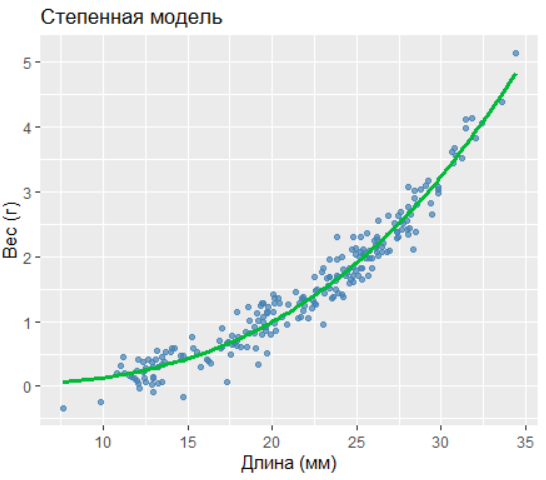
\includegraphics[width=0.6\linewidth,height=\textheight,keepaspectratio]{images/power_shrimp.PNG}
  \end{center}
\end{itemize}

\subsubsection{\texorpdfstring{\textbf{3. Сравнение
моделей}}{3. Сравнение моделей}}\label{ux441ux440ux430ux432ux43dux435ux43dux438ux435-ux43cux43eux434ux435ux43bux435ux439-1}

\begin{longtable}[]{@{}lll@{}}
\toprule\noalign{}
\textbf{Модель} & \textbf{R²} & \textbf{AIC} \\
\midrule\noalign{}
\endhead
\bottomrule\noalign{}
\endlastfoot
Линейная & 0.894 & 148.02 \\
Полиномиальная & 0.957 & -52.80 \\
Степенная & 0.955 & -48.43 \\
\end{longtable}

\textbf{Выводы:}

\begin{enumerate}
\def\labelenumi{\arabic{enumi}.}
\item
  \textbf{Полиномиальная модель} демонстрирует наилучшие показатели
  (максимальный R² и минимальный AIC).
\item
  \textbf{Степенная модель} близка по качеству, но её параметр
  \emph{b}≈2.92 близок к биологически ожидаемому значению 3 (вес
  пропорционален объёму).
\item
  \textbf{Линейная модель} существенно уступает по точности.
\end{enumerate}

\subsubsection{\texorpdfstring{\textbf{4.
Рекомендации}}{4. Рекомендации}}\label{ux440ux435ux43aux43eux43cux435ux43dux434ux430ux446ux438ux438}

\begin{itemize}
\item
  \textbf{Для прогнозирования} используйте полиномиальную модель, так
  как она минимизирует ошибку.
\item
  \textbf{Для биологической интерпретации} предпочтительна степенная
  модель: weight∝length\textsuperscript{2.92}.
\item
  \textbf{Избегайте переобучения:} Полиномиальные модели высокой степени
  могут терять интерпретируемость.
\end{itemize}

\subsubsection{\texorpdfstring{\textbf{5. Визуализация
остатков}}{5. Визуализация остатков}}\label{ux432ux438ux437ux443ux430ux43bux438ux437ux430ux446ux438ux44f-ux43eux441ux442ux430ux442ux43aux43eux432}

Остатки степенной модели распределены равномерно, что подтверждает её
адекватность: \begin{center}
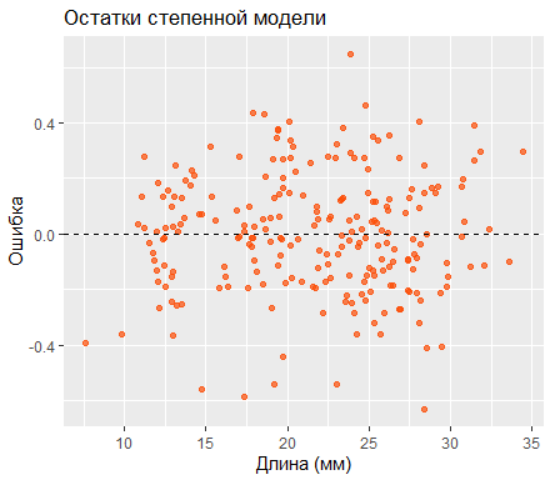
\includegraphics[width=0.6\linewidth,height=\textheight,keepaspectratio]{images/residuals_shrimp.PNG}
\end{center}

\subsubsection{\texorpdfstring{\textbf{Заключение}}{Заключение}}\label{ux437ux430ux43aux43bux44eux447ux435ux43dux438ux435}

Для анализа зависимости веса от длины северной креветки
\textbf{рекомендуется}:

\begin{enumerate}
\def\labelenumi{\arabic{enumi}.}
\item
  \textbf{Полиномиальная модель} --- для задач, требующих максимальной
  точности.
\item
  \textbf{Степенная модель} --- для интерпретации биологических
  закономерностей.
\end{enumerate}

Скрипт вышеописанных событий:

\begin{Shaded}
\begin{Highlighting}[]
\CommentTok{\# Установка рабочей директории}
\FunctionTok{setwd}\NormalTok{(}\StringTok{"C:/TEXTBOOK/"}\NormalTok{)}

\CommentTok{\# Загрузка библиотек}
\FunctionTok{library}\NormalTok{(tidyverse)}
\FunctionTok{library}\NormalTok{(ggplot2)}

\CommentTok{\# Загрузка данных}
\NormalTok{data }\OtherTok{\textless{}{-}} \FunctionTok{read\_csv}\NormalTok{(}\StringTok{"shrimp\_catch.csv"}\NormalTok{) }\SpecialCharTok{\%\textgreater{}\%}
  \FunctionTok{filter}\NormalTok{(}\SpecialCharTok{!}\NormalTok{id }\SpecialCharTok{\%in\%} \FunctionTok{c}\NormalTok{(}\DecValTok{10}\NormalTok{, }\DecValTok{50}\NormalTok{))  }\CommentTok{\# Удаление аномальных наблюдений}

\CommentTok{\# Проверка структуры}
\FunctionTok{glimpse}\NormalTok{(data)}

\CommentTok{\# Линейная модель: вес \textasciitilde{} длина}
\NormalTok{model\_linear }\OtherTok{\textless{}{-}} \FunctionTok{lm}\NormalTok{(weight }\SpecialCharTok{\textasciitilde{}}\NormalTok{ length, }\AttributeTok{data =}\NormalTok{ data)}
\FunctionTok{summary}\NormalTok{(model\_linear)}

\CommentTok{\# Визуализация}
\FunctionTok{ggplot}\NormalTok{(data, }\FunctionTok{aes}\NormalTok{(}\AttributeTok{x =}\NormalTok{ length, }\AttributeTok{y =}\NormalTok{ weight)) }\SpecialCharTok{+}
  \FunctionTok{geom\_point}\NormalTok{(}\AttributeTok{color =} \StringTok{"steelblue"}\NormalTok{, }\AttributeTok{alpha =} \FloatTok{0.7}\NormalTok{) }\SpecialCharTok{+}
  \FunctionTok{geom\_smooth}\NormalTok{(}\AttributeTok{method =} \StringTok{"lm"}\NormalTok{, }\AttributeTok{color =} \StringTok{"\#FC4E07"}\NormalTok{) }\SpecialCharTok{+}
  \FunctionTok{labs}\NormalTok{(}\AttributeTok{title =} \StringTok{"Линейная модель"}\NormalTok{, }\AttributeTok{x =} \StringTok{"Длина (мм)"}\NormalTok{, }\AttributeTok{y =} \StringTok{"Вес (г)"}\NormalTok{)}


\CommentTok{\# Полиномиальная модель: вес \textasciitilde{} длина + длина? + длина?}
\NormalTok{model\_poly }\OtherTok{\textless{}{-}} \FunctionTok{lm}\NormalTok{(weight }\SpecialCharTok{\textasciitilde{}} \FunctionTok{poly}\NormalTok{(length, }\DecValTok{3}\NormalTok{), }\AttributeTok{data =}\NormalTok{ data)}
\FunctionTok{summary}\NormalTok{(model\_poly)}

\CommentTok{\# Визуализация}
\FunctionTok{ggplot}\NormalTok{(data, }\FunctionTok{aes}\NormalTok{(}\AttributeTok{x =}\NormalTok{ length, }\AttributeTok{y =}\NormalTok{ weight)) }\SpecialCharTok{+}
  \FunctionTok{geom\_point}\NormalTok{(}\AttributeTok{color =} \StringTok{"steelblue"}\NormalTok{, }\AttributeTok{alpha =} \FloatTok{0.7}\NormalTok{) }\SpecialCharTok{+}
  \FunctionTok{geom\_smooth}\NormalTok{(}\AttributeTok{method =} \StringTok{"lm"}\NormalTok{, }\AttributeTok{formula =}\NormalTok{ y }\SpecialCharTok{\textasciitilde{}} \FunctionTok{poly}\NormalTok{(x, }\DecValTok{3}\NormalTok{), }\AttributeTok{color =} \StringTok{"\#E7B800"}\NormalTok{) }\SpecialCharTok{+}
  \FunctionTok{labs}\NormalTok{(}\AttributeTok{title =} \StringTok{"Полиномиальная модель"}\NormalTok{, }\AttributeTok{x =} \StringTok{"Длина (мм)"}\NormalTok{, }\AttributeTok{y =} \StringTok{"Вес (г)"}\NormalTok{)}


\CommentTok{\# Степенная модель: вес \textasciitilde{} длина\^{}k (k подбирается)}
\NormalTok{model\_power }\OtherTok{\textless{}{-}} \FunctionTok{nls}\NormalTok{(weight }\SpecialCharTok{\textasciitilde{}}\NormalTok{ a }\SpecialCharTok{*}\NormalTok{ length}\SpecialCharTok{\^{}}\NormalTok{b, }
                   \AttributeTok{data =}\NormalTok{ data, }
                   \AttributeTok{start =} \FunctionTok{list}\NormalTok{(}\AttributeTok{a =} \FloatTok{0.001}\NormalTok{, }\AttributeTok{b =} \DecValTok{3}\NormalTok{))  }\CommentTok{\# Начальные значения}
\FunctionTok{summary}\NormalTok{(model\_power)}

\CommentTok{\# Визуализация}
\NormalTok{data}\SpecialCharTok{$}\NormalTok{pred\_power }\OtherTok{\textless{}{-}} \FunctionTok{predict}\NormalTok{(model\_power)}
\FunctionTok{ggplot}\NormalTok{(data, }\FunctionTok{aes}\NormalTok{(}\AttributeTok{x =}\NormalTok{ length, }\AttributeTok{y =}\NormalTok{ weight)) }\SpecialCharTok{+}
  \FunctionTok{geom\_point}\NormalTok{(}\AttributeTok{color =} \StringTok{"steelblue"}\NormalTok{, }\AttributeTok{alpha =} \FloatTok{0.7}\NormalTok{) }\SpecialCharTok{+}
  \FunctionTok{geom\_line}\NormalTok{(}\FunctionTok{aes}\NormalTok{(}\AttributeTok{y =}\NormalTok{ pred\_power), }\AttributeTok{color =} \StringTok{"\#00BA38"}\NormalTok{, }\AttributeTok{linewidth =} \FloatTok{1.2}\NormalTok{) }\SpecialCharTok{+}
  \FunctionTok{labs}\NormalTok{(}\AttributeTok{title =} \StringTok{"Степенная модель"}\NormalTok{, }\AttributeTok{x =} \StringTok{"Длина (мм)"}\NormalTok{, }\AttributeTok{y =} \StringTok{"Вес (г)"}\NormalTok{)}

\CommentTok{\# Расчет AIC}
\FunctionTok{AIC}\NormalTok{(model\_linear, model\_poly, model\_power)}

\CommentTok{\# Расчет R?}
\NormalTok{r2\_linear }\OtherTok{\textless{}{-}} \FunctionTok{summary}\NormalTok{(model\_linear)}\SpecialCharTok{$}\NormalTok{r.squared}
\NormalTok{r2\_poly }\OtherTok{\textless{}{-}} \FunctionTok{summary}\NormalTok{(model\_poly)}\SpecialCharTok{$}\NormalTok{r.squared}
\NormalTok{r2\_power }\OtherTok{\textless{}{-}} \DecValTok{1} \SpecialCharTok{{-}} \FunctionTok{sum}\NormalTok{(}\FunctionTok{residuals}\NormalTok{(model\_power)}\SpecialCharTok{\^{}}\DecValTok{2}\NormalTok{) }\SpecialCharTok{/} \FunctionTok{sum}\NormalTok{((data}\SpecialCharTok{$}\NormalTok{weight }\SpecialCharTok{{-}} \FunctionTok{mean}\NormalTok{(data}\SpecialCharTok{$}\NormalTok{weight))}\SpecialCharTok{\^{}}\DecValTok{2}\NormalTok{)}

\CommentTok{\# Создание таблицы сравнения моделей}
\NormalTok{comparison\_table }\OtherTok{\textless{}{-}} \FunctionTok{data.frame}\NormalTok{(}
\NormalTok{  Модель }\OtherTok{=} \FunctionTok{c}\NormalTok{(}\StringTok{"Линейная"}\NormalTok{, }\StringTok{"Полиномиальная"}\NormalTok{, }\StringTok{"Степенная"}\NormalTok{),}
  \AttributeTok{R\_square =} \FunctionTok{c}\NormalTok{(r2\_linear, r2\_poly, r2\_power),}
  \AttributeTok{AIC =} \FunctionTok{c}\NormalTok{(}\FunctionTok{AIC}\NormalTok{(model\_linear), }\FunctionTok{AIC}\NormalTok{(model\_poly), }\FunctionTok{AIC}\NormalTok{(model\_power))}
\NormalTok{)}

\CommentTok{\# Вывод таблицы}
\FunctionTok{print}\NormalTok{(comparison\_table)}

\CommentTok{\# Остатки для степенной модели}
\NormalTok{data}\SpecialCharTok{$}\NormalTok{residuals }\OtherTok{\textless{}{-}} \FunctionTok{residuals}\NormalTok{(model\_power)}

\FunctionTok{ggplot}\NormalTok{(data, }\FunctionTok{aes}\NormalTok{(}\AttributeTok{x =}\NormalTok{ length, }\AttributeTok{y =}\NormalTok{ residuals)) }\SpecialCharTok{+}
  \FunctionTok{geom\_point}\NormalTok{(}\AttributeTok{color =} \StringTok{"\#FC4E07"}\NormalTok{, }\AttributeTok{alpha =} \FloatTok{0.7}\NormalTok{) }\SpecialCharTok{+}
  \FunctionTok{geom\_hline}\NormalTok{(}\AttributeTok{yintercept =} \DecValTok{0}\NormalTok{, }\AttributeTok{linetype =} \StringTok{"dashed"}\NormalTok{) }\SpecialCharTok{+}
  \FunctionTok{labs}\NormalTok{(}\AttributeTok{title =} \StringTok{"Остатки степенной модели"}\NormalTok{, }\AttributeTok{x =} \StringTok{"Длина (мм)"}\NormalTok{, }\AttributeTok{y =} \StringTok{"Ошибка"}\NormalTok{)}
\end{Highlighting}
\end{Shaded}

\bookmarksetup{startatroot}

\chapter{Нейронные сети в экологии: практическое
введение}\label{ux43dux435ux439ux440ux43eux43dux43dux44bux435-ux441ux435ux442ux438-ux432-ux44dux43aux43eux43bux43eux433ux438ux438-ux43fux440ux430ux43aux442ux438ux447ux435ux441ux43aux43eux435-ux432ux432ux435ux434ux435ux43dux438ux435}

\section{Введение}\label{ux432ux432ux435ux434ux435ux43dux438ux435-1}

Это практическое занятие можно рассматривать не только как введение в
нейронные сети, но и как введение в экологическое моделирование в общем
с помошью R. Занятие основано на статье Андрея Викторовича Коросова
``\href{https://ecopri.ru/journal/article.php?id=14002}{Нейронные сети в
экологии: введение}'', опубликованной в журнале Принципы экологии, №3,
2023, стр. 76-96. В статье рассмотрены основы нейросетевого
моделирования в экологии, начиная с классических регрессионных методов и
заканчивая искусственными нейронными сетями. Представленные примеры
демонстрируют эволюционный переход от простых линейных моделей к сложным
нейросетевым конструкциям, что позволяет решать задачи классификации и
прогнозирования в экологии. ``Теоретическая'' лекция, основанная на этой
статье, находиться по \href{KOROSOV.ppt}{ссылке}.

Можно скачать скрипт целиком в трех версиях:
\href{https://mombus.github.io/cRab/data/KOROSOV.R}{KOROSOV.R} -
максимально приближен к оригинальной работе;
\href{https://mombus.github.io/cRab/data/KOROSOV_updated.R}{KOROSOV\_updated.R}
- тотже скрипт, но с комментариями и пояснениями (содержание этого
занятия);
\href{https://mombus.github.io/cRab/data/KOROSOV_visual.R}{KOROSOV\_visual.R}
- почти такой же с дополнительным продвинутым визуалом и аналитикой.

\subsubsection{\texorpdfstring{\textbf{Для работы
скрипта:}}{Для работы скрипта:}}\label{ux434ux43bux44f-ux440ux430ux431ux43eux442ux44b-ux441ux43aux440ux438ux43fux442ux430}

\begin{enumerate}
\def\labelenumi{\arabic{enumi}.}
\item
  Скачайте файлы данных
  (\href{https://mombus.github.io/cRab/data/vipkar.csv}{vipkar.csv} и
  \href{https://mombus.github.io/cRab/data/kihzsdat.csv}{kihzsdat.csv})
\item
  Установите рабочую директорию в setwd()
\item
  Установите необходимые пакеты :
  \textbf{\texttt{install.packages(c("neuralnet",\ "ggplot2"))}}
\end{enumerate}

\begin{Shaded}
\begin{Highlighting}[]
\CommentTok{\# ЗАГРУЗКА БИБЛИОТЕК И НАСТРОЙКА СРЕДЫ ================================}
\FunctionTok{library}\NormalTok{(neuralnet)   }\CommentTok{\# Для построения нейронных сетей}
\FunctionTok{library}\NormalTok{(ggplot2)     }\CommentTok{\# Для продвинутой визуализации (в данном скрипте не используется напрямую)}

\CommentTok{\# Установите свою рабочую директорию (где лежат файлы данных)}
\CommentTok{\# setwd("C:/ВАША\_ДИРЕКТОРИЯ/")}
\end{Highlighting}
\end{Shaded}

\section{ЛИНЕЙНАЯ
РЕГРЕССИЯ}\label{ux43bux438ux43dux435ux439ux43dux430ux44f-ux440ux435ux433ux440ux435ux441ux441ux438ux44f}

В этом разделе мы изучим основы экологического моделирования на примере
зависимости массы тела гадюки от ее длины. Вы построите простую линейную
регрессионную модель, визуализируете данные и линию регрессии, а также
интерпретируете результаты с помощью функции \texttt{summary()}.

Загружаем данные

\begin{Shaded}
\begin{Highlighting}[]
\CommentTok{\# Данные: масса (w) и длина тела (lt) гадюк (в см и граммах)}
\NormalTok{w }\OtherTok{\textless{}{-}} \FunctionTok{c}\NormalTok{(}\DecValTok{85}\NormalTok{, }\DecValTok{90}\NormalTok{, }\DecValTok{85}\NormalTok{, }\DecValTok{95}\NormalTok{, }\DecValTok{95}\NormalTok{, }\DecValTok{135}\NormalTok{, }\DecValTok{165}\NormalTok{, }\DecValTok{135}\NormalTok{, }\DecValTok{140}\NormalTok{)}
\NormalTok{lt }\OtherTok{\textless{}{-}} \FunctionTok{c}\NormalTok{(}\DecValTok{51}\NormalTok{, }\DecValTok{51}\NormalTok{, }\DecValTok{52}\NormalTok{, }\DecValTok{54}\NormalTok{, }\DecValTok{54}\NormalTok{, }\DecValTok{59}\NormalTok{, }\DecValTok{59}\NormalTok{, }\DecValTok{60}\NormalTok{, }\DecValTok{62}\NormalTok{)}
\end{Highlighting}
\end{Shaded}

Строим и запускаем модель \[
w_t = a_0 + a_1 \cdot l_t
\]

где: - \(w_t\) --- зависимая переменная, - \(a_0\) --- свободный член, -
\(a_1\) --- коэффициент регрессии, - \(l_t\) --- независимая переменная.

\begin{Shaded}
\begin{Highlighting}[]
\CommentTok{\# Построение линейной модели: w = a0 + a1*lt}
\NormalTok{lreg }\OtherTok{\textless{}{-}} \FunctionTok{lm}\NormalTok{(w }\SpecialCharTok{\textasciitilde{}}\NormalTok{ lt)}
\end{Highlighting}
\end{Shaded}

Выведем результаты модели

\begin{Shaded}
\begin{Highlighting}[]
\CommentTok{\# Просмотр результатов модели:}
\FunctionTok{summary}\NormalTok{(lreg)  }\CommentTok{\# Обратите внимание на коэффициенты и p{-}значения}
\end{Highlighting}
\end{Shaded}

На экране появится:

\begin{Shaded}
\begin{Highlighting}[]
\NormalTok{Call}\SpecialCharTok{:}
\FunctionTok{lm}\NormalTok{(}\AttributeTok{formula =}\NormalTok{ w }\SpecialCharTok{\textasciitilde{}}\NormalTok{ lt)}

\NormalTok{Residuals}\SpecialCharTok{:}
\NormalTok{    Min      }\DecValTok{1}\NormalTok{Q  Median      }\DecValTok{3}\NormalTok{Q     Max }
\SpecialCharTok{{-}}\FloatTok{13.452}  \SpecialCharTok{{-}}\FloatTok{7.585}  \SpecialCharTok{{-}}\FloatTok{4.868}   \FloatTok{1.490}  \FloatTok{30.623} 

\NormalTok{Coefficients}\SpecialCharTok{:}
\NormalTok{            Estimate Std. Error t value }\FunctionTok{Pr}\NormalTok{(}\SpecialCharTok{\textgreater{}}\ErrorTok{|}\NormalTok{t}\SpecialCharTok{|}\NormalTok{)    }
\NormalTok{(Intercept) }\SpecialCharTok{{-}}\FloatTok{240.766}     \FloatTok{64.457}  \SpecialCharTok{{-}}\FloatTok{3.735} \FloatTok{0.007308} \SpecialCharTok{**} 
\NormalTok{lt             }\FloatTok{6.358}      \FloatTok{1.153}   \FloatTok{5.516} \FloatTok{0.000891} \SpecialCharTok{**}\ErrorTok{*}
\SpecialCharTok{{-}{-}{-}}
\NormalTok{Signif. codes}\SpecialCharTok{:}  \DecValTok{0}\NormalTok{ ‘}\SpecialCharTok{**}\ErrorTok{*}\NormalTok{’ }\FloatTok{0.001}\NormalTok{ ‘}\SpecialCharTok{**}\NormalTok{’ }\FloatTok{0.01}\NormalTok{ ‘}\SpecialCharTok{*}\NormalTok{’ }\FloatTok{0.05}\NormalTok{ ‘.’ }\FloatTok{0.1}\NormalTok{ ‘ ’ }\DecValTok{1}

\NormalTok{Residual standard error}\SpecialCharTok{:} \FloatTok{13.81}\NormalTok{ on }\DecValTok{7}\NormalTok{ degrees of freedom}
\NormalTok{Multiple R}\SpecialCharTok{{-}}\NormalTok{squared}\SpecialCharTok{:}  \FloatTok{0.813}\NormalTok{,     Adjusted R}\SpecialCharTok{{-}}\NormalTok{squared}\SpecialCharTok{:}  \FloatTok{0.7863} 
\NormalTok{F}\SpecialCharTok{{-}}\NormalTok{statistic}\SpecialCharTok{:} \FloatTok{30.43}\NormalTok{ on }\DecValTok{1}\NormalTok{ and }\DecValTok{7}\NormalTok{ DF,  p}\SpecialCharTok{{-}}\NormalTok{value}\SpecialCharTok{:} \FloatTok{0.0008911}
\end{Highlighting}
\end{Shaded}

Мы получили результаты линейной регрессии, где зависимая переменная ---
масса тела гадюки (w), а независимая переменная --- длина тела (lt).
Разберем каждый параметр:

1. **Call (Вызов модели):**

`lm(formula = w \textasciitilde{} lt)`

Это просто напоминание, какая модель была построена. Здесь указано, что
мы моделировали зависимость массы (w) от длины тела (lt) с помощью
линейной регрессии.

2. **Residuals (Остатки):**

Остатки --- это разница между наблюдаемыми значениями массы и
предсказанными моделью значениями. Они показывают, насколько хорошо
модель описывает данные.

\begin{itemize}
\item
  `Min`: минимальный остаток = -13.452 (наибольшее недооцененное
  значение)
\item
  `1Q`: первый квартиль = -7.585 (25\% остатков меньше этого значения)
\item
  `Median`: медиана остатков = -4.868 (середина распределения остатков)
\item
  `3Q`: третий квартиль = 1.490 (75\% остатков меньше этого значения)
\item
  `Max`: максимальный остаток = 30.623 (наибольшее переоцененное
  значение)
\end{itemize}

Распределение остатков: медиана немного смещена влево (отрицательное
значение), а размах между 1Q и 3Q составляет примерно 9 единиц. Это
может указывать на легкую асимметрию, но выборка мала.

3. **Coefficients (Коэффициенты):**

\begin{itemize}
\item
  `(Intercept)`: свободный член (a0) = -240.766. Это предсказанное
  значение массы при длине тела, равной нулю. Биологически это не имеет
  смысла (длина не может быть нулевой), но это математическая
  особенность модели.
\item
  `lt`: коэффициент регрессии (a1) = 6.358. Это означает, что при
  увеличении длины тела на 1 см масса тела увеличивается в среднем на
  6.358 г.
\end{itemize}

Для каждого коэффициента приведены:

\begin{itemize}
\item
  `Estimate`: точечная оценка коэффициента.
\item
  `Std. Error`: стандартная ошибка оценки коэффициента. Для intercept =
  64.457, для lt = 1.153. Это мера изменчивости оценки.
\item
  `t value`: t-статистика. Рассчитывается как Estimate / Std.Error. Для
  intercept: -240.766 / 64.457 ≈ -3.735; для lt: 6.358 / 1.153 ≈ 5.516.
\item
  `Pr(\textgreater\textbar t\textbar)`: p-значение для проверки гипотезы
  о равенстве коэффициента нулю.
\item
  Для intercept: p=0.007308 (значим на уровне α=0.01, т.е. intercept
  статистически значимо отличается от нуля).
\item
  Для lt: p=0.000891 (значим на уровне α=0.001). Это означает, что длина
  тела значимо влияет на массу.
\end{itemize}

Значимость кодов: три звездочки (`***`) означают, что коэффициент значим
на уровне 0.001.

4. **Residual standard error (Стандартная ошибка остатков):** 13.81 на 7
степенях свободы. Это мера разброса остатков. В среднем, предсказания
модели отклоняются от реальных значений на ±13.81 г. Степени свободы
(df) = n - 2 = 9 - 2 = 7 (n --- количество наблюдений).

5. **Multiple R-squared (Коэффициент детерминации R²):** 0.813. Это
означает, что 81.3\% вариации массы тела объясняется длиной тела.
Остальные 18.7\% --- это неучтенные факторы и случайная изменчивость.

6. **Adjusted R-squared (Скорректированный R²):** 0.7863. Этот
показатель корректирует R² с учетом числа предикторов. Он полезен при
сравнении моделей с разным числом предикторов. Здесь он немного меньше
R², так как учитывает, что в модели один предиктор.

7. **F-statistic (F-статистика):** 30.43 на 1 и 7 степенях свободы.
Проверяет гипотезу о том, что все коэффициенты (кроме intercept) равны
нулю (т.е. модель не лучше, чем модель только с константой).

\begin{itemize}
\tightlist
\item
  p-value: 0.0008911 (крайне значимый), что означает, что модель в целом
  адекватна.
\end{itemize}

**Выводы:**

- Уравнение модели: `w = -240.77 + 6.36 * lt`

- Длина тела значимо влияет на массу (p\textless0.001).

- Модель объясняет 81.3\% вариации массы.

- На каждый сантиметр длины тела масса увеличивается примерно на 6.36 г.

- Остатки модели показывают, что есть несколько точек, которые модель
предсказывает с заметной ошибкой (особенно максимальный остаток в 30.6
г). Возможно, для более точного прогноза нужна нелинейная модель или
учет дополнительных факторов.

**Рекомендации:**

- Проверить допущения линейной регрессии (нормальность остатков,
гомоскедастичность) с помощью диагностических графиков.

- Рассмотреть возможность включения других переменных (например,
возраста, пола) в модель.

- Убедиться, что в данных нет выбросов, которые могут влиять на
коэффициенты.

\begin{Shaded}
\begin{Highlighting}[]
\CommentTok{\# Визуализация зависимости}
\FunctionTok{plot}\NormalTok{(lt, w, }
     \AttributeTok{main =} \StringTok{"Зависимость массы от длины тела гадюки"}\NormalTok{, }
     \AttributeTok{xlab =} \StringTok{"Длина тела (см)"}\NormalTok{, }
     \AttributeTok{ylab =} \StringTok{"Масса (г)"}\NormalTok{, }
     \AttributeTok{pch =} \DecValTok{19}\NormalTok{,        }\CommentTok{\# Кружки вместо стандартных точек}
     \AttributeTok{col =} \StringTok{"darkgreen"}\NormalTok{)}
\FunctionTok{abline}\NormalTok{(lreg, }\AttributeTok{col =} \StringTok{"red"}\NormalTok{, }\AttributeTok{lwd =} \DecValTok{2}\NormalTok{)  }\CommentTok{\# Добавляем линию регрессии}
\end{Highlighting}
\end{Shaded}

\begin{figure}[H]

{\centering 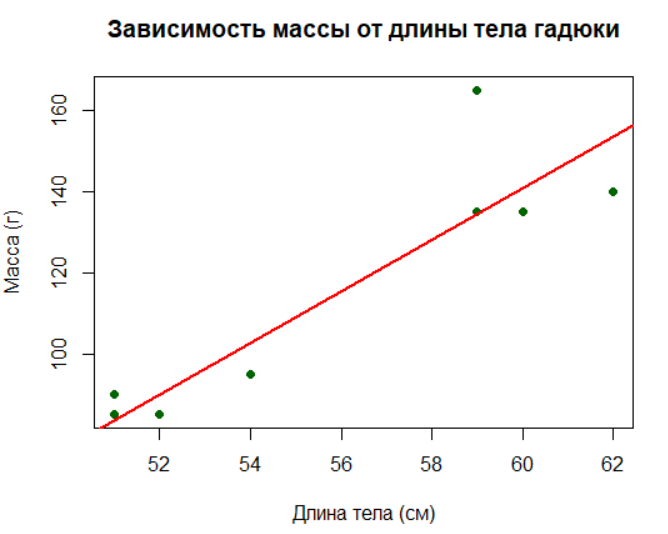
\includegraphics[width=0.6\linewidth,height=\textheight,keepaspectratio]{images/KOROSOV1.PNG}

}

\caption{Рис. 1.: Пример линейной регрессии}

\end{figure}%

\section{ЧИСЛЕННАЯ
ОПТИМИЗАЦИЯ}\label{ux447ux438ux441ux43bux435ux43dux43dux430ux44f-ux43eux43fux442ux438ux43cux438ux437ux430ux446ux438ux44f}

Здесь вы познакомитесь с численными методами оптимизации параметров
моделей, которые применяются, когда аналитическое решение невозможно. На
примере той же зависимости массы от длины вы подгоните параметры модели
с помощью функции \texttt{nls()} и сравните результаты с аналитическим
решением.

Аналитические методы дают точное решение в виде математической формулы,
используя алгебраические преобразования и теоремы математического
анализа. Они идеальны для простых моделей, где существуют явные решения,
обеспечивая прозрачную интерпретацию параметров. В экологии такие методы
применимы для базовых зависимостей типа линейной регрессии. Численные
методы используются, когда аналитическое решение невозможно, и работают
через последовательные приближения, начиная со стартовых значений и
итеративно улучшая параметры модели. Они незаменимы для сложных
экологических моделей с нелинейными зависимостями, взаимодействиями
факторов и ``шумными'' полевыми данными, позволяя решать задачи,
недоступные для аналитических подходов.

\begin{Shaded}
\begin{Highlighting}[]
\CommentTok{\# Подгонка параметров через оптимизацию}
\NormalTok{nls\_model }\OtherTok{\textless{}{-}} \FunctionTok{nls}\NormalTok{(w }\SpecialCharTok{\textasciitilde{}}\NormalTok{ a0 }\SpecialCharTok{+}\NormalTok{ a1 }\SpecialCharTok{*}\NormalTok{ lt, }\AttributeTok{start =} \FunctionTok{list}\NormalTok{(}\AttributeTok{a0 =} \DecValTok{1}\NormalTok{, }\AttributeTok{a1 =} \DecValTok{1}\NormalTok{))}
\FunctionTok{summary}\NormalTok{(nls\_model)}
\end{Highlighting}
\end{Shaded}

На экране появится:

\begin{Shaded}
\begin{Highlighting}[]
\NormalTok{Formula}\SpecialCharTok{:}\NormalTok{ w }\SpecialCharTok{\textasciitilde{}}\NormalTok{ a0 }\SpecialCharTok{+}\NormalTok{ a1 }\SpecialCharTok{*}\NormalTok{ lt}

\NormalTok{Parameters}\SpecialCharTok{:}
\NormalTok{   Estimate Std. Error t value }\FunctionTok{Pr}\NormalTok{(}\SpecialCharTok{\textgreater{}}\ErrorTok{|}\NormalTok{t}\SpecialCharTok{|}\NormalTok{)    }
\NormalTok{a0 }\SpecialCharTok{{-}}\FloatTok{240.766}     \FloatTok{64.457}  \SpecialCharTok{{-}}\FloatTok{3.735} \FloatTok{0.007308} \SpecialCharTok{**} 
\NormalTok{a1    }\FloatTok{6.358}      \FloatTok{1.153}   \FloatTok{5.516} \FloatTok{0.000891} \SpecialCharTok{**}\ErrorTok{*}
\SpecialCharTok{{-}{-}{-}}
\NormalTok{Signif. codes}\SpecialCharTok{:}  \DecValTok{0}\NormalTok{ ‘}\SpecialCharTok{**}\ErrorTok{*}\NormalTok{’ }\FloatTok{0.001}\NormalTok{ ‘}\SpecialCharTok{**}\NormalTok{’ }\FloatTok{0.01}\NormalTok{ ‘}\SpecialCharTok{*}\NormalTok{’ }\FloatTok{0.05}\NormalTok{ ‘.’ }\FloatTok{0.1}\NormalTok{ ‘ ’ }\DecValTok{1}

\NormalTok{Residual standard error}\SpecialCharTok{:} \FloatTok{13.81}\NormalTok{ on }\DecValTok{7}\NormalTok{ degrees of freedom}

\NormalTok{Number of iterations to convergence}\SpecialCharTok{:} \DecValTok{1} 
\NormalTok{Achieved convergence tolerance}\SpecialCharTok{:} \FloatTok{3.247e{-}08}
\end{Highlighting}
\end{Shaded}

\subsection{\texorpdfstring{\textbf{Интерпретация результатов
модели}}{Интерпретация результатов модели}}\label{ux438ux43dux442ux435ux440ux43fux440ux435ux442ux430ux446ux438ux44f-ux440ux435ux437ux443ux43bux44cux442ux430ux442ux43eux432-ux43cux43eux434ux435ux43bux438}

Мы построили линейную модель зависимости массы гадюки (w) от длины её
тела (lt) по формуле:\\
\textbf{\texttt{w\ =\ a0\ +\ a1\ *\ lt}}

\textbf{Ключевые параметры модели:}

\begin{itemize}
\item
  \textbf{a0 (свободный член)}: -240.8 г\\
  Это теоретическая масса при нулевой длине тела. Отрицательное значение
  указывает, что модель не подходит для очень молодых особей.
\item
  \textbf{a1 (коэффициент при lt)}: 6.36 г/см\\
  Каждый дополнительный сантиметр длины тела увеличивает массу в среднем
  на 6.36 г.
\end{itemize}

\textbf{Точность и значимость:}

\begin{itemize}
\item
  Оба коэффициента \textbf{высоко значимы} (p \textless{} 0.01), что
  подтверждает реальность зависимости.
\item
  Стандартная ошибка для a1 составляет 1.15 г/см - это значит, что
  реальное значение, вероятно, находится между 5.2 и 7.5 г/см.
\item
  Модель хорошо сошлась за 1 шаг (итерацию), что говорит об удачном
  подборе параметров.
\end{itemize}

\textbf{Ошибка прогноза:}\\
Среднее отклонение предсказаний от реальных значений - 13.8 г
(стандартная ошибка остатков). Для особи массой 100 г это означает
возможную ошибку прогноза около 14\%.

\begin{quote}
\textbf{Биологический смысл:} Модель подтверждает сильную аллометрию -
крупные гадюки имеют относительно большую массу тела. Каждый сантиметр
длины добавляет около 6.4 г массы. Для особи длиной 55 см прогнозируемая
масса составит: -240.8 + 6.36*55 ≈ 109 г.
\end{quote}

\#\#МНОЖЕСТВЕННАЯ РЕГРЕССИЯ

В этом разделе мы расширим модель, включив несколько факторов. Вы
построите множественную регрессию, учитывающую одновременно длину тела и
длину хвоста гадюки, и научитесь интерпретировать влияние нескольких
предикторов на зависимую переменную.

\begin{Shaded}
\begin{Highlighting}[]
\CommentTok{\# Добавляем новый признак {-} длину хвоста (lc)}
\NormalTok{w }\OtherTok{\textless{}{-}} \FunctionTok{c}\NormalTok{(}\DecValTok{40}\NormalTok{, }\DecValTok{156}\NormalTok{, }\DecValTok{105}\NormalTok{, }\DecValTok{85}\NormalTok{, }\DecValTok{80}\NormalTok{, }\DecValTok{50}\NormalTok{, }\DecValTok{75}\NormalTok{, }\DecValTok{48}\NormalTok{, }\DecValTok{75}\NormalTok{, }\DecValTok{67}\NormalTok{)}
\NormalTok{lt }\OtherTok{\textless{}{-}} \FunctionTok{c}\NormalTok{(}\DecValTok{44}\NormalTok{, }\DecValTok{59}\NormalTok{, }\DecValTok{49}\NormalTok{, }\DecValTok{50}\NormalTok{, }\DecValTok{54}\NormalTok{, }\DecValTok{43}\NormalTok{, }\DecValTok{49}\NormalTok{, }\DecValTok{42}\NormalTok{, }\DecValTok{47}\NormalTok{, }\DecValTok{47}\NormalTok{)}
\NormalTok{lc }\OtherTok{\textless{}{-}} \FunctionTok{c}\NormalTok{(}\DecValTok{70}\NormalTok{, }\DecValTok{78}\NormalTok{, }\DecValTok{66}\NormalTok{, }\DecValTok{90}\NormalTok{, }\DecValTok{83}\NormalTok{, }\DecValTok{70}\NormalTok{, }\DecValTok{62}\NormalTok{, }\DecValTok{75}\NormalTok{, }\DecValTok{40}\NormalTok{, }\DecValTok{80}\NormalTok{)}
\end{Highlighting}
\end{Shaded}

Используя glm-функцию, построим модель с двумя предикторами: \[
w = a_0 + a_1 \cdot l_t + a_2 \cdot l_c
\]

где: - \(w\) --- масса гадюки, - \(l_t\) --- длина тела гадюки, -
\(l_c\) --- длина хвоста гадюки, - \(a_0\) --- свободный член
(константа), - \(a_1\) --- коэффициент регрессии при длине тела, -
\(a_2\) --- коэффициент регрессии при длине хвоста.

\begin{Shaded}
\begin{Highlighting}[]
\CommentTok{\# Множественная регрессия: w = a0 + a1*lt + a2*lc}
\NormalTok{multi\_reg }\OtherTok{\textless{}{-}} \FunctionTok{glm}\NormalTok{(w }\SpecialCharTok{\textasciitilde{}}\NormalTok{ lt }\SpecialCharTok{+}\NormalTok{ lc)}
\FunctionTok{summary}\NormalTok{(multi\_reg)}
\end{Highlighting}
\end{Shaded}

На экране появится:

\begin{Shaded}
\begin{Highlighting}[]
\NormalTok{Call}\SpecialCharTok{:}
\FunctionTok{glm}\NormalTok{(}\AttributeTok{formula =}\NormalTok{ w }\SpecialCharTok{\textasciitilde{}}\NormalTok{ lt }\SpecialCharTok{+}\NormalTok{ lc)}

\NormalTok{Coefficients}\SpecialCharTok{:}
\NormalTok{             Estimate Std. Error t value }\FunctionTok{Pr}\NormalTok{(}\SpecialCharTok{\textgreater{}}\ErrorTok{|}\NormalTok{t}\SpecialCharTok{|}\NormalTok{)    }
\NormalTok{(Intercept) }\SpecialCharTok{{-}}\FloatTok{191.2982}    \FloatTok{53.6908}  \SpecialCharTok{{-}}\FloatTok{3.563} \FloatTok{0.009183} \SpecialCharTok{**} 
\NormalTok{lt             }\FloatTok{6.0308}     \FloatTok{1.1051}   \FloatTok{5.457} \FloatTok{0.000949} \SpecialCharTok{**}\ErrorTok{*}
\NormalTok{lc            }\SpecialCharTok{{-}}\FloatTok{0.3150}     \FloatTok{0.4133}  \SpecialCharTok{{-}}\FloatTok{0.762} \FloatTok{0.470913}    
\SpecialCharTok{{-}{-}{-}}
\NormalTok{Signif. codes}\SpecialCharTok{:}  \DecValTok{0}\NormalTok{ ‘}\SpecialCharTok{**}\ErrorTok{*}\NormalTok{’ }\FloatTok{0.001}\NormalTok{ ‘}\SpecialCharTok{**}\NormalTok{’ }\FloatTok{0.01}\NormalTok{ ‘}\SpecialCharTok{*}\NormalTok{’ }\FloatTok{0.05}\NormalTok{ ‘.’ }\FloatTok{0.1}\NormalTok{ ‘ ’ }\DecValTok{1}

\NormalTok{(Dispersion parameter }\ControlFlowTok{for}\NormalTok{ gaussian family taken to be }\FloatTok{270.9752}\NormalTok{)}

\NormalTok{    Null deviance}\SpecialCharTok{:} \FloatTok{10132.9}\NormalTok{  on }\DecValTok{9}\NormalTok{  degrees of freedom}
\NormalTok{Residual deviance}\SpecialCharTok{:}  \FloatTok{1896.8}\NormalTok{  on }\DecValTok{7}\NormalTok{  degrees of freedom}
\NormalTok{AIC}\SpecialCharTok{:} \FloatTok{88.832}

\NormalTok{Number of Fisher Scoring iterations}\SpecialCharTok{:} \DecValTok{2}
\end{Highlighting}
\end{Shaded}

\subsection{\texorpdfstring{\textbf{Интерпретация результатов
множественной
регрессии}}{Интерпретация результатов множественной регрессии}}\label{ux438ux43dux442ux435ux440ux43fux440ux435ux442ux430ux446ux438ux44f-ux440ux435ux437ux443ux43bux44cux442ux430ux442ux43eux432-ux43cux43dux43eux436ux435ux441ux442ux432ux435ux43dux43dux43eux439-ux440ux435ux433ux440ux435ux441ux441ux438ux438}

Мы исследовали зависимость массы гадюки (w) от длины тела (lt) и длины
хвоста (lc) с помощью модели:\\
\textbf{\texttt{w\ =\ b0\ +\ b1*lt\ +\ b2*lc}}

\textbf{Ключевые выводы модели:}

\begin{enumerate}
\def\labelenumi{\arabic{enumi}.}
\item
  \textbf{Длина тела (lt) сильно влияет на массу}:

  \begin{itemize}
  \item
    Коэффициент: +6.03 г/см
  \item
    Каждый сантиметр длины тела увеличивает массу на \textasciitilde6 г
  \item
    Высокая значимость (p = 0.00095)
  \end{itemize}
\item
  \textbf{Длина хвоста (lc) не влияет значимо на массу}:

  \begin{itemize}
  \item
    Коэффициент: -0.315 г/см (незначимый)
  \item
    p-значение 0.47 \textgreater{} 0.05 - статистически недостоверно
  \item
    После учета длины тела, длина хвоста не добавляет информации
  \end{itemize}
\item
  \textbf{Свободный член (b0)}: -191.3 г\\
  Отрицательное значение подтверждает нелинейность роста у молодых
  особей
\end{enumerate}

\textbf{Качество модели:}

\begin{itemize}
\item
  Модель объясняет значительную часть вариации:\\
  Общая вариация (Null deviance) = 10132.9\\
  Остаточная вариация (Residual deviance) = 1896.8 → \textbf{Объяснено
  81\% вариации}
\item
  AIC = 88.8 (ниже, чем у модели без lc - 92.1, что указывает на лучшее
  качество)
\item
  Модель быстро сошлась за 2 итерации
\end{itemize}

\textbf{Биологическая интерпретация:}

\begin{enumerate}
\def\labelenumi{\arabic{enumi}.}
\item
  Масса тела определяется в основном длиной туловища, а не хвоста
\item
  Для прогноза массы достаточно учитывать только длину тела
\item
  Пример прогноза для особи (lt=50 см, lc=70 см):\\
  \textbf{\texttt{-191.3\ +\ 6.03*50\ -\ 0.315*70\ ≈\ 111\ г}}
\end{enumerate}

\begin{quote}
\textbf{Рекомендация}: При изучении массы гадюк можно исключить длину
хвоста из модели, так как она не вносит значимого вклада в предсказание.
Основным морфометрическим показателем остается длина тела.
\end{quote}

\section{НЕЛИНЕЙНЫЕ
ЗАВИСИМОСТИ}\label{ux43dux435ux43bux438ux43dux435ux439ux43dux44bux435-ux437ux430ux432ux438ux441ux438ux43cux43eux441ux442ux438}

Экологические данные часто имеют нелинейный характер. Здесь вы
смоделируете степенную зависимость (аллометрию) между массой и длиной
тела, используя линеаризацию через логарифмирование, а затем
визуализируете кривую модели.

\begin{Shaded}
\begin{Highlighting}[]
\CommentTok{\# Часто в экологии связи имеют степенной характер: w = a0 * lt\^{}a1}
\CommentTok{\# Линеаризация через логарифмирование}
\NormalTok{log\_model }\OtherTok{\textless{}{-}} \FunctionTok{lm}\NormalTok{(}\FunctionTok{log}\NormalTok{(w) }\SpecialCharTok{\textasciitilde{}} \FunctionTok{log}\NormalTok{(lt))}

\CommentTok{\# Преобразование коэффициентов обратно}
\NormalTok{a0 }\OtherTok{\textless{}{-}} \FunctionTok{exp}\NormalTok{(}\FunctionTok{coef}\NormalTok{(log\_model)[}\DecValTok{1}\NormalTok{])  }\CommentTok{\# Переход от логарифмов}
\NormalTok{a1 }\OtherTok{\textless{}{-}} \FunctionTok{coef}\NormalTok{(log\_model)[}\DecValTok{2}\NormalTok{]       }\CommentTok{\# Показатель степени}

\CommentTok{\# Визуализация степенной зависимости}
\FunctionTok{plot}\NormalTok{(lt, w, }
     \AttributeTok{main =} \StringTok{"Степенная зависимость массы от длины"}\NormalTok{, }
     \AttributeTok{xlab =} \StringTok{"Длина тела (см)"}\NormalTok{, }
     \AttributeTok{ylab =} \StringTok{"Масса (г)"}\NormalTok{,}
     \AttributeTok{pch =} \DecValTok{17}\NormalTok{,}
     \AttributeTok{col =} \StringTok{"blue"}\NormalTok{)}
\FunctionTok{curve}\NormalTok{(a0 }\SpecialCharTok{*}\NormalTok{ x}\SpecialCharTok{\^{}}\NormalTok{a1, }\AttributeTok{add =} \ConstantTok{TRUE}\NormalTok{, }\AttributeTok{col =} \StringTok{"red"}\NormalTok{, }\AttributeTok{lwd =} \DecValTok{2}\NormalTok{)  }\CommentTok{\# Кривая модели}
\end{Highlighting}
\end{Shaded}

\begin{figure}[H]

{\centering 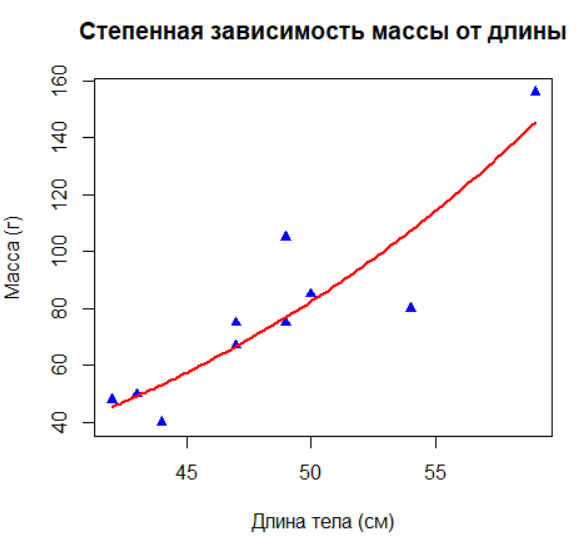
\includegraphics[width=0.6\linewidth,height=\textheight,keepaspectratio]{images/KOROSOV2.PNG}

}

\caption{Рис. 2.: Расчет степенной функции}

\end{figure}%

\section{ЛОГИСТИЧЕСКАЯ
РЕГРЕССИЯ}\label{ux43bux43eux433ux438ux441ux442ux438ux447ux435ux441ux43aux430ux44f-ux440ux435ux433ux440ux435ux441ux441ux438ux44f}

Вы изучите моделирование пороговых эффектов в экологии на примере
смертности дафний в зависимости от концентрации токсиканта. Построив
логистическую регрессию, вы получите S-образную кривую, характерную для
таких процессов.

\begin{Shaded}
\begin{Highlighting}[]
\CommentTok{\# Пример: смертность дафний при разных концентрациях токсиканта}
\CommentTok{\# Данные:}
\NormalTok{K }\OtherTok{\textless{}{-}} \FunctionTok{c}\NormalTok{(}\DecValTok{100}\NormalTok{, }\DecValTok{126}\NormalTok{, }\DecValTok{158}\NormalTok{, }\DecValTok{200}\NormalTok{, }\DecValTok{251}\NormalTok{, }\DecValTok{316}\NormalTok{, }\DecValTok{398}\NormalTok{, }\DecValTok{501}\NormalTok{, }\DecValTok{631}\NormalTok{, }\DecValTok{794}\NormalTok{, }\DecValTok{1000}\NormalTok{)}
\NormalTok{p }\OtherTok{\textless{}{-}} \FunctionTok{c}\NormalTok{(}\DecValTok{0}\NormalTok{, }\DecValTok{0}\NormalTok{, }\DecValTok{0}\NormalTok{, }\DecValTok{0}\NormalTok{, }\DecValTok{0}\NormalTok{, }\FloatTok{0.5}\NormalTok{, }\FloatTok{0.5}\NormalTok{, }\DecValTok{1}\NormalTok{, }\DecValTok{1}\NormalTok{, }\DecValTok{1}\NormalTok{, }\DecValTok{1}\NormalTok{)  }\CommentTok{\# Доля погибших}
\NormalTok{d }\OtherTok{\textless{}{-}} \FunctionTok{data.frame}\NormalTok{(K, p)}

\CommentTok{\# Построение логистической модели}
\NormalTok{logit\_model }\OtherTok{\textless{}{-}} \FunctionTok{glm}\NormalTok{(p }\SpecialCharTok{\textasciitilde{}}\NormalTok{ K, }\AttributeTok{family =} \FunctionTok{binomial}\NormalTok{(), }\AttributeTok{data =}\NormalTok{ d)}

\CommentTok{\# Визуализация S{-}образной кривой}
\FunctionTok{plot}\NormalTok{(d}\SpecialCharTok{$}\NormalTok{K, d}\SpecialCharTok{$}\NormalTok{p, }
     \AttributeTok{xlab =} \StringTok{"Концентрация токсиканта (мг/л)"}\NormalTok{, }
     \AttributeTok{ylab =} \StringTok{"Доля погибших"}\NormalTok{, }
     \AttributeTok{main =} \StringTok{"Токсическое воздействие на дафний"}\NormalTok{,}
     \AttributeTok{pch =} \DecValTok{19}\NormalTok{,}
     \AttributeTok{col =} \StringTok{"red"}\NormalTok{)}
\FunctionTok{lines}\NormalTok{(d}\SpecialCharTok{$}\NormalTok{K, }\FunctionTok{predict}\NormalTok{(logit\_model, }\AttributeTok{type =} \StringTok{"response"}\NormalTok{), }
      \AttributeTok{col =} \StringTok{"blue"}\NormalTok{, }\AttributeTok{lwd =} \DecValTok{2}\NormalTok{, }\AttributeTok{lty =} \DecValTok{1}\NormalTok{)}
\end{Highlighting}
\end{Shaded}

\begin{figure}[H]

{\centering 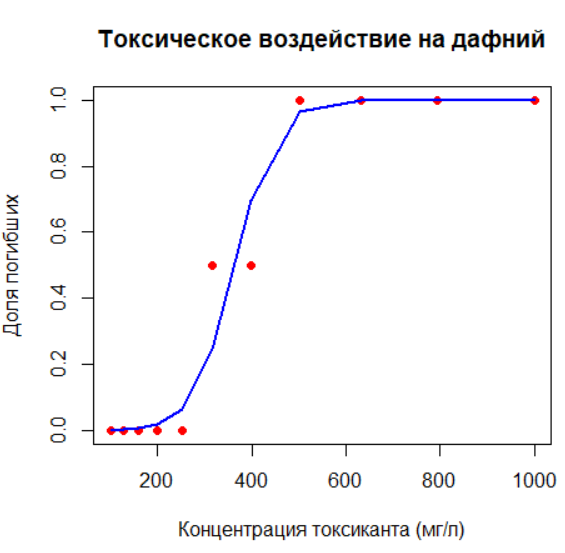
\includegraphics[width=0.6\linewidth,height=\textheight,keepaspectratio]{images/KOROSOV3.PNG}

}

\caption{Рис. 3.: Расчет логистической регрессии гибели дафний в
токсиканте}

\end{figure}%

\section{ПЕРЕХОД К
СЕТЯМ}\label{ux43fux435ux440ux435ux445ux43eux434-ux43a-ux441ux435ux442ux44fux43c}

Сделаем первый шаг к нейронным сетям, построив простейшую сеть без
скрытых слоев (аналог линейной регрессии) для модели токсичности. Вы
визуализируете структуру сети и убедитесь, что она дает результат,
аналогичный линейной модели.

\begin{Shaded}
\begin{Highlighting}[]
\CommentTok{\# Простейшая нейросеть (аналог линейной регрессии)}
\NormalTok{nn\_simple }\OtherTok{\textless{}{-}} \FunctionTok{neuralnet}\NormalTok{(p }\SpecialCharTok{\textasciitilde{}}\NormalTok{ K, }\AttributeTok{data =}\NormalTok{ d, }\AttributeTok{hidden =} \DecValTok{0}\NormalTok{)}

\CommentTok{\# Визуализация структуры сети}
\FunctionTok{plot}\NormalTok{(nn\_simple, }\AttributeTok{rep =} \StringTok{"best"}\NormalTok{)}
\end{Highlighting}
\end{Shaded}

\begin{figure}[H]

{\centering 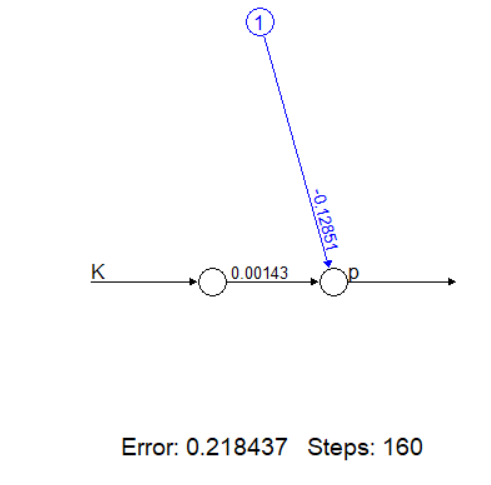
\includegraphics[width=0.4\linewidth,height=\textheight,keepaspectratio]{images/KOROSOV4.PNG}

}

\caption{Рис. 4.: Схема нейрона}

\end{figure}%

\section{НЕЙРОНЫ КАК НЕЛИНЕЙНЫЕ
ПРЕОБРАЗОВАТЕЛИ}\label{ux43dux435ux439ux440ux43eux43dux44b-ux43aux430ux43a-ux43dux435ux43bux438ux43dux435ux439ux43dux44bux435-ux43fux440ux435ux43eux431ux440ux430ux437ux43eux432ux430ux442ux435ux43bux438}

Здесь вы добавите в нейронную сеть скрытый слой с одним нейроном, что
позволит моделировать нелинейные зависимости. Вы сравните результат
работы такой сети с логистической регрессией и увидите, как нейронная
сеть имитирует пороговый эффект.

\begin{Shaded}
\begin{Highlighting}[]
\CommentTok{\# Сеть с одним скрытым нейроном (имитирует логистическую регрессию)}
\NormalTok{nn\_1hidden }\OtherTok{\textless{}{-}} \FunctionTok{neuralnet}\NormalTok{(p }\SpecialCharTok{\textasciitilde{}}\NormalTok{ K, }\AttributeTok{data =}\NormalTok{ d, }\AttributeTok{hidden =} \DecValTok{1}\NormalTok{)}

\CommentTok{\# Сравнение с логистической регрессией}
\FunctionTok{plot}\NormalTok{(d}\SpecialCharTok{$}\NormalTok{K, }\FunctionTok{predict}\NormalTok{(logit\_model, }\AttributeTok{type =} \StringTok{"response"}\NormalTok{), }
     \AttributeTok{type =} \StringTok{"l"}\NormalTok{, }
     \AttributeTok{col =} \StringTok{"darkgreen"}\NormalTok{, }
     \AttributeTok{lwd =} \DecValTok{2}\NormalTok{,}
     \AttributeTok{xlab =} \StringTok{"Концентрация"}\NormalTok{, }
     \AttributeTok{ylab =} \StringTok{"Смертность"}\NormalTok{,}
     \AttributeTok{main =} \StringTok{"Сравнение моделей"}\NormalTok{)}
\FunctionTok{lines}\NormalTok{(d}\SpecialCharTok{$}\NormalTok{K, }\FunctionTok{predict}\NormalTok{(nn\_1hidden, d), }\AttributeTok{col =} \StringTok{"blue"}\NormalTok{, }\AttributeTok{lty =} \DecValTok{2}\NormalTok{, }\AttributeTok{lwd =} \DecValTok{2}\NormalTok{)}
\FunctionTok{legend}\NormalTok{(}\StringTok{"bottomright"}\NormalTok{, }
       \AttributeTok{legend =} \FunctionTok{c}\NormalTok{(}\StringTok{"Логистическая регрессия"}\NormalTok{, }\StringTok{"Нейронная сеть (1 нейрон)"}\NormalTok{),}
       \AttributeTok{col =} \FunctionTok{c}\NormalTok{(}\StringTok{"darkgreen"}\NormalTok{, }\StringTok{"blue"}\NormalTok{), }
       \AttributeTok{lty =} \DecValTok{1}\SpecialCharTok{:}\DecValTok{2}\NormalTok{,}
       \AttributeTok{lwd =} \DecValTok{2}\NormalTok{)}
\end{Highlighting}
\end{Shaded}

\begin{figure}[H]

{\centering 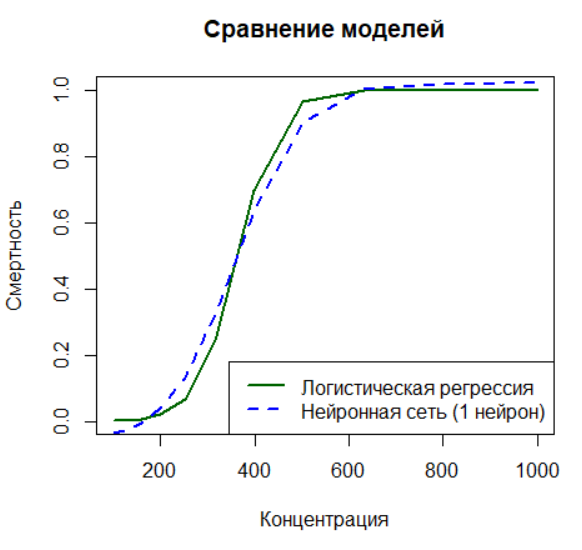
\includegraphics[width=0.4\linewidth,height=\textheight,keepaspectratio]{images/KOROSOV5.PNG}

}

\caption{Рис. 5.: Сравнение работы}

\end{figure}%

\section{КЛАССИФИКАЦИЯ В
ЭКОЛОГИИ}\label{ux43aux43bux430ux441ux441ux438ux444ux438ux43aux430ux446ux438ux44f-ux432-ux44dux43aux43eux43bux43eux433ux438ux438}

Вы примените нейронные сети для решения задачи классификации -
определения пола гадюк по морфометрическим признакам. Построив и сравнив
несколько архитектур сетей (без скрытых нейронов, с одним и тремя
нейронами), вы оцените их точность.

\begin{Shaded}
\begin{Highlighting}[]
\CommentTok{\# Загрузка данных по гадюкам (пол, длина тела, длина хвоста, масса)}
\NormalTok{v }\OtherTok{\textless{}{-}} \FunctionTok{read.csv}\NormalTok{(}\StringTok{"vipkar.csv"}\NormalTok{)}
\FunctionTok{head}\NormalTok{(v, }\DecValTok{3}\NormalTok{)  }\CommentTok{\# Просмотр первых строк данных}
\end{Highlighting}
\end{Shaded}

Модель без скрытых нейронов (аналог линейной регрессии)

\begin{Shaded}
\begin{Highlighting}[]
\NormalTok{nv0 }\OtherTok{\textless{}{-}} \FunctionTok{neuralnet}\NormalTok{(ns }\SpecialCharTok{\textasciitilde{}}\NormalTok{ lc, }\AttributeTok{data =}\NormalTok{ v, }\AttributeTok{hidden =} \DecValTok{0}\NormalTok{)}
\FunctionTok{plot}\NormalTok{(nv0)  }\CommentTok{\# Визуализация простейшей сети}
\end{Highlighting}
\end{Shaded}

\begin{figure}[H]

{\centering 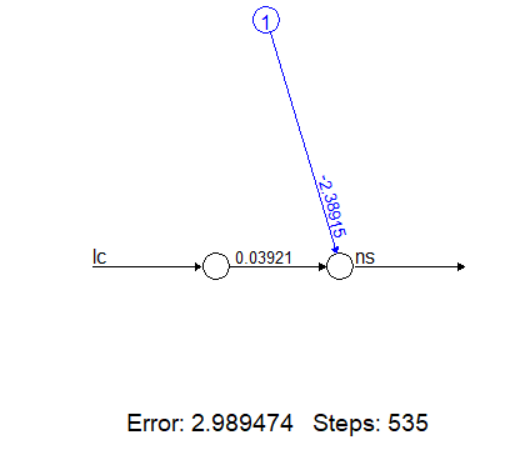
\includegraphics[width=0.4\linewidth,height=\textheight,keepaspectratio]{images/KOROSOV6.PNG}

}

\caption{Рис. 6.: Визуализация простейшей сети}

\end{figure}%

Модель с одним скрытым нейроном

\begin{Shaded}
\begin{Highlighting}[]
\NormalTok{nv1 }\OtherTok{\textless{}{-}} \FunctionTok{neuralnet}\NormalTok{(ns }\SpecialCharTok{\textasciitilde{}}\NormalTok{ lc, }\AttributeTok{data =}\NormalTok{ v, }\AttributeTok{hidden =} \DecValTok{1}\NormalTok{)}
\FunctionTok{plot}\NormalTok{(nv1)  }\CommentTok{\# Схема сети с одним нейроном}
\end{Highlighting}
\end{Shaded}

\begin{figure}[H]

{\centering 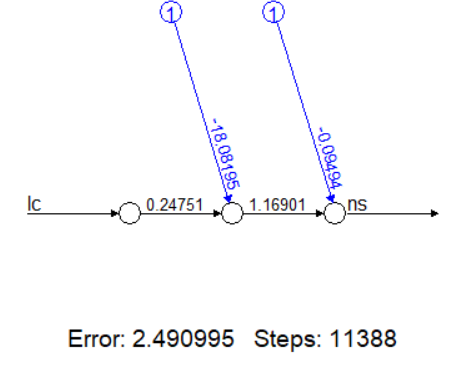
\includegraphics[width=0.4\linewidth,height=\textheight,keepaspectratio]{images/KOROSOV7.PNG}

}

\caption{Рис. 7.: Схема сети с одним нейроном}

\end{figure}%

Модель с тремя скрытыми нейронами (полноценная нейросеть)

\begin{Shaded}
\begin{Highlighting}[]
\NormalTok{nv3 }\OtherTok{\textless{}{-}} \FunctionTok{neuralnet}\NormalTok{(ns }\SpecialCharTok{\textasciitilde{}}\NormalTok{ lc }\SpecialCharTok{+}\NormalTok{ lt }\SpecialCharTok{+}\NormalTok{ w, }\AttributeTok{data =}\NormalTok{ v, }\AttributeTok{hidden =} \DecValTok{3}\NormalTok{)}
\FunctionTok{plot}\NormalTok{(nv3)  }\CommentTok{\# Визуализация сложной сети}
\end{Highlighting}
\end{Shaded}

\begin{figure}[H]

{\centering 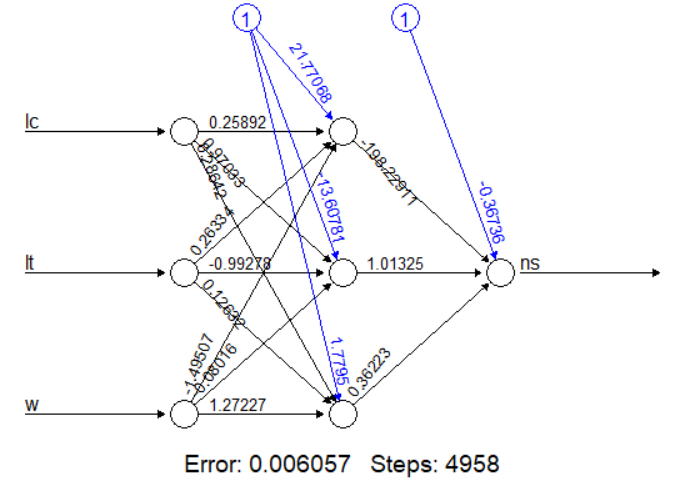
\includegraphics[width=0.4\linewidth,height=\textheight,keepaspectratio]{images/KOROSOV8.PNG}

}

\caption{Рис. 8.: Модель с тремя скрытыми нейронами}

\end{figure}%

Оценка точности классификации

\begin{Shaded}
\begin{Highlighting}[]
\NormalTok{predictions }\OtherTok{\textless{}{-}} \FunctionTok{predict}\NormalTok{(nv3, v)}
\NormalTok{predicted\_sex }\OtherTok{\textless{}{-}} \FunctionTok{round}\NormalTok{(predictions)}
\NormalTok{accuracy }\OtherTok{\textless{}{-}} \FunctionTok{mean}\NormalTok{(v}\SpecialCharTok{$}\NormalTok{ns }\SpecialCharTok{==}\NormalTok{ predicted\_sex)}
\FunctionTok{cat}\NormalTok{(}\StringTok{"Точность классификации:"}\NormalTok{, }\FunctionTok{round}\NormalTok{(accuracy}\SpecialCharTok{*}\DecValTok{100}\NormalTok{, }\DecValTok{1}\NormalTok{), }\StringTok{"\%}\SpecialCharTok{\textbackslash{}n}\StringTok{"}\NormalTok{)}
\end{Highlighting}
\end{Shaded}

Сравнение разных архитектур нейронных сетей (см. срипт
\href{https://mombus.github.io/cRab/data/KOROSOV_visual.R}{KOROSOV\_visual.R})

\begin{figure}[H]

{\centering 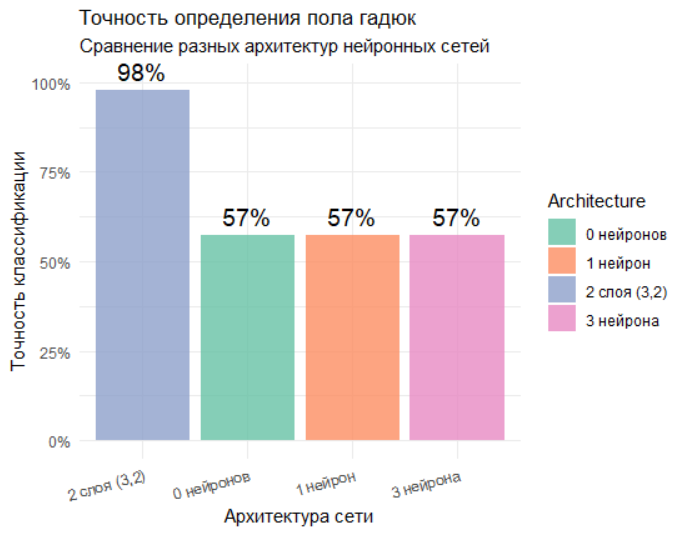
\includegraphics[width=0.6\linewidth,height=\textheight,keepaspectratio]{images/KOROSOV9.PNG}

}

\caption{Рис. 9.: Точность определения пола гадюк}

\end{figure}%

\section{ПРОСТРАНСТВЕННОЕ
МОДЕЛИРОВАНИЕ}\label{ux43fux440ux43eux441ux442ux440ux430ux43dux441ux442ux432ux435ux43dux43dux43eux435-ux43cux43eux434ux435ux43bux438ux440ux43eux432ux430ux43dux438ux435}

В завершение вы построите нейронную сеть для прогнозирования численности
гадюк на островах по характеристикам биотопов. Вы разделите данные на
обучающую и тестовую выборки, оцените точность модели и используете ее
для прогноза в новых условиях.

\begin{Shaded}
\begin{Highlighting}[]
\CommentTok{\# Данные по островам Кижского архипелага}
\NormalTok{v }\OtherTok{\textless{}{-}} \FunctionTok{read.csv}\NormalTok{(}\StringTok{"kihzsdat.csv"}\NormalTok{)}
\FunctionTok{head}\NormalTok{(v, }\DecValTok{3}\NormalTok{)  }\CommentTok{\# Структура данных: площадь, биотопы, численность видов}

\CommentTok{\# Случайное разделение данных на обучающую и тестовую выборки}
\FunctionTok{set.seed}\NormalTok{(}\DecValTok{123}\NormalTok{)  }\CommentTok{\# Для воспроизводимости}
\NormalTok{train\_indices }\OtherTok{\textless{}{-}} \FunctionTok{sample}\NormalTok{(}\DecValTok{1}\SpecialCharTok{:}\FunctionTok{nrow}\NormalTok{(v), }\DecValTok{12}\NormalTok{)}
\NormalTok{train\_data }\OtherTok{\textless{}{-}}\NormalTok{ v[train\_indices, ]}
\NormalTok{test\_data }\OtherTok{\textless{}{-}}\NormalTok{ v[}\SpecialCharTok{{-}}\NormalTok{train\_indices, ]}

\CommentTok{\# Построение нейросети с 5 нейронами в скрытом слое}
\NormalTok{model }\OtherTok{\textless{}{-}} \FunctionTok{neuralnet}\NormalTok{(vb }\SpecialCharTok{\textasciitilde{}}\NormalTok{ fo }\SpecialCharTok{+}\NormalTok{ me }\SpecialCharTok{+}\NormalTok{ bo, }\AttributeTok{data =}\NormalTok{ train\_data, }\AttributeTok{hidden =} \DecValTok{5}\NormalTok{)}

\CommentTok{\# Прогнозирование на обучающей выборке}
\NormalTok{train\_pred }\OtherTok{\textless{}{-}} \FunctionTok{predict}\NormalTok{(model, train\_data)}
\NormalTok{train\_accuracy }\OtherTok{\textless{}{-}} \FunctionTok{mean}\NormalTok{(}\FunctionTok{round}\NormalTok{(train\_pred) }\SpecialCharTok{==}\NormalTok{ train\_data}\SpecialCharTok{$}\NormalTok{vb)}
\FunctionTok{cat}\NormalTok{(}\StringTok{"Точность на обучающей выборке:"}\NormalTok{, }\FunctionTok{round}\NormalTok{(train\_accuracy}\SpecialCharTok{*}\DecValTok{100}\NormalTok{, }\DecValTok{1}\NormalTok{), }\StringTok{"\%}\SpecialCharTok{\textbackslash{}n}\StringTok{"}\NormalTok{)}

\CommentTok{\# Прогнозирование на тестовой выборке}
\NormalTok{test\_pred }\OtherTok{\textless{}{-}} \FunctionTok{predict}\NormalTok{(model, test\_data)}
\NormalTok{test\_accuracy }\OtherTok{\textless{}{-}} \FunctionTok{mean}\NormalTok{(}\FunctionTok{round}\NormalTok{(test\_pred) }\SpecialCharTok{==}\NormalTok{ test\_data}\SpecialCharTok{$}\NormalTok{vb)}
\FunctionTok{cat}\NormalTok{(}\StringTok{"Точность на тестовой выборке:"}\NormalTok{, }\FunctionTok{round}\NormalTok{(test\_accuracy}\SpecialCharTok{*}\DecValTok{100}\NormalTok{, }\DecValTok{1}\NormalTok{), }\StringTok{"\%}\SpecialCharTok{\textbackslash{}n}\StringTok{"}\NormalTok{)}

\CommentTok{\# Прогноз для новых условий (пример)}
\NormalTok{new\_conditions }\OtherTok{\textless{}{-}} \FunctionTok{data.frame}\NormalTok{(}
  \AttributeTok{fo =} \FunctionTok{c}\NormalTok{(}\FloatTok{57.9}\NormalTok{, }\FloatTok{35.3}\NormalTok{, }\FloatTok{83.0}\NormalTok{),  }\CommentTok{\# Площадь лесов (\%)}
  \AttributeTok{me =} \FunctionTok{c}\NormalTok{(}\FloatTok{4.1}\NormalTok{, }\FloatTok{0.0}\NormalTok{, }\FloatTok{7.3}\NormalTok{),     }\CommentTok{\# Площадь лугов (\%)}
  \AttributeTok{bo =} \FunctionTok{c}\NormalTok{(}\FloatTok{3.4}\NormalTok{, }\FloatTok{7.9}\NormalTok{, }\FloatTok{11.5}\NormalTok{)     }\CommentTok{\# Площадь болот (\%)}
\NormalTok{)}

\NormalTok{future\_pred }\OtherTok{\textless{}{-}} \FunctionTok{predict}\NormalTok{(model, new\_conditions)}
\FunctionTok{cat}\NormalTok{(}\StringTok{"Прогнозируемая численность гадюк:"}\NormalTok{, }\FunctionTok{round}\NormalTok{(future\_pred), }\StringTok{"}\SpecialCharTok{\textbackslash{}n}\StringTok{"}\NormalTok{)}
\end{Highlighting}
\end{Shaded}

\bookmarksetup{startatroot}

\chapter{Основы
картографии}\label{ux43eux441ux43dux43eux432ux44b-ux43aux430ux440ux442ux43eux433ux440ux430ux444ux438ux438}

\section{Введение}\label{ux432ux432ux435ux434ux435ux43dux438ux435-2}

Примеры карт и скрипты, которые могут быть полезны в рыбохозяйственных,
гидробиологическских и пр. океанологических исследованиях. На этом
занятии мы рассмотрим создание карт для визуализации пространственных
данных в исследованиях водных биоресурсов.

Вы научитесь создавать различные типы карт, используя современные пакеты
R, такие как \texttt{ggplot2}, \texttt{sf}, \texttt{rnaturalearth} и
другие. Мы начнем с простых карт распределения уловов по данным съемок,
затем перейдем к более сложным: картам с береговой линией, картам,
включающим нулевые уловы, распределению по квартилям. Далее рассмотрим
фасеточные карты для сравнения лет, карты с пространственной
автокорреляцией (LISA), а также промысловые карты (включая картограммы)
и гибридные карты, объединяющие данные съемок и промысла. В заключение
мы покажем, как создавать карты для раздела ``Материал и методы'' и
карты с врезками.

Обратите внимание, что примеры карт, представленные в интернете
(например, в HTML-версии этого документа), могут быть в уменьшенном
качестве. Однако при работе в R вы можете экспортировать полученные
графики в векторные (PDF, SVG) или растровые (PNG, TIFF) форматы с
высоким разрешением (до 600 dpi), что подходит для публикаций в научных
журналах.

\textbf{Для работы скрипта:}

\begin{enumerate}
\def\labelenumi{\arabic{enumi}.}
\item
  Скачайте файл данных
  (\href{https://mombus.github.io/cRab/data/KARTOGRAPHIC.xlsx}{KARTOGRAPHIC.xlsx})
\item
  Установите рабочую директорию в setwd()
\item
  Установите необходимые пакеты :
  \textbf{\texttt{install.packages(c("readxl",\ "tidyverse,\ "rnaturalearth",\ "sf",\ "viridis"\ ))}}
  \texttt{и\ др.}
\end{enumerate}

\section{Карта распределения уловов в
съемке}\label{ux43aux430ux440ux442ux430-ux440ux430ux441ux43fux440ux435ux434ux435ux43bux435ux43dux438ux44f-ux443ux43bux43eux432ux43eux432-ux432-ux441ux44aux435ux43cux43aux435}

Данная карта демонстрирует распределение уловов краба в ходе
исследовательской съемки. На ней отображены точки наблюдений, где размер
и цвет точек соответствуют величине улова.

\begin{figure}[H]

{\centering 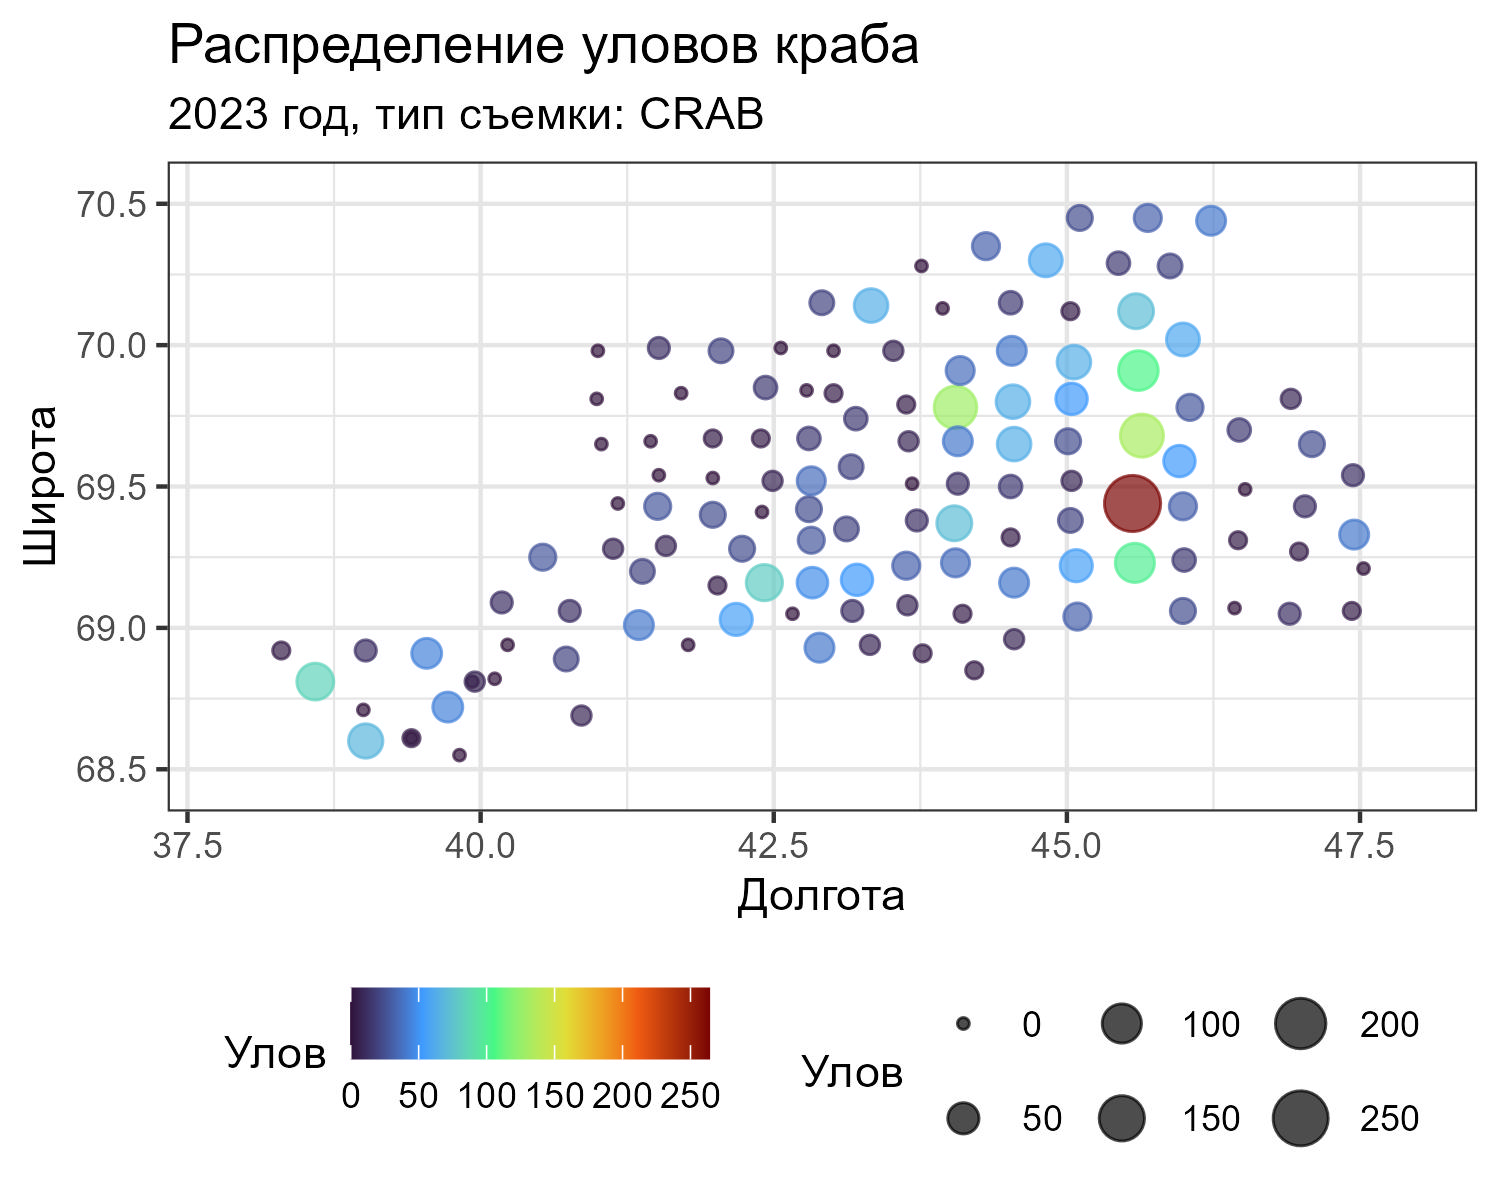
\includegraphics[width=0.7\linewidth,height=\textheight,keepaspectratio]{images/KARTOGRAPH1.jpg}

}

\caption{Рис. 1.: Пример карты распределения уловов в съемке}

\end{figure}%

В скрипте границы карты (лимиты) определяются автоматически с буфером,
но чаще их просто устанавливают вручную, например:

\begin{Shaded}
\begin{Highlighting}[]
\NormalTok{xmin }\OtherTok{\textless{}{-}} \DecValTok{37}
\NormalTok{xmax }\OtherTok{\textless{}{-}} \DecValTok{49}
\NormalTok{ymin }\OtherTok{\textless{}{-}} \FloatTok{68.5}
\NormalTok{ymax }\OtherTok{\textless{}{-}} \FloatTok{70.5}
\end{Highlighting}
\end{Shaded}

Скрипт карты целиком:

\begin{Shaded}
\begin{Highlighting}[]
\CommentTok{\# Очистка памяти и установка рабочей папки}
\FunctionTok{rm}\NormalTok{(}\AttributeTok{list =} \FunctionTok{ls}\NormalTok{())}
\FunctionTok{setwd}\NormalTok{(}\StringTok{"C:/COURSES/KARTOGRAPH/"}\NormalTok{)}

\CommentTok{\# Загрузка необходимых пакетов}
\FunctionTok{library}\NormalTok{(tidyverse)  }\CommentTok{\# Обработка данных и визуализация}
\FunctionTok{library}\NormalTok{(readxl)     }\CommentTok{\# Чтение Excel{-}файлов}

\CommentTok{\# 1. ЗАГРУЗКА ДАННЫХ}
\NormalTok{DATA }\OtherTok{\textless{}{-}} \FunctionTok{read\_excel}\NormalTok{(}\StringTok{"KARTOGRAPHIC.xlsx"}\NormalTok{, }\AttributeTok{sheet =} \StringTok{"SURVEY"}\NormalTok{) }\SpecialCharTok{\%\textgreater{}\%} 
  \FunctionTok{filter}\NormalTok{(YEAR }\SpecialCharTok{==} \DecValTok{2023}\NormalTok{, SURV }\SpecialCharTok{==} \StringTok{"CRAB"}\NormalTok{)  }\CommentTok{\# Фильтр для 2023 года и съемки CRAB}

\CommentTok{\# 2. АВТОМАТИЧЕСКИЙ РАСЧЕТ ГРАНИЦ С БУФЕРОМ 5\%}
\CommentTok{\# Расчет диапазонов координат}
\NormalTok{x\_range }\OtherTok{\textless{}{-}} \FunctionTok{range}\NormalTok{(DATA}\SpecialCharTok{$}\NormalTok{X, }\AttributeTok{na.rm =} \ConstantTok{TRUE}\NormalTok{)}
\NormalTok{y\_range }\OtherTok{\textless{}{-}} \FunctionTok{range}\NormalTok{(DATA}\SpecialCharTok{$}\NormalTok{Y, }\AttributeTok{na.rm =} \ConstantTok{TRUE}\NormalTok{)}

\CommentTok{\# Расчет 5\% буфера}
\NormalTok{x\_buffer }\OtherTok{\textless{}{-}} \FloatTok{0.05} \SpecialCharTok{*} \FunctionTok{diff}\NormalTok{(x\_range)}
\NormalTok{y\_buffer }\OtherTok{\textless{}{-}} \FloatTok{0.05} \SpecialCharTok{*} \FunctionTok{diff}\NormalTok{(y\_range)}

\CommentTok{\# Установка границ с буфером}
\NormalTok{xmin }\OtherTok{\textless{}{-}}\NormalTok{ x\_range[}\DecValTok{1}\NormalTok{] }\SpecialCharTok{{-}}\NormalTok{ x\_buffer}
\NormalTok{xmax }\OtherTok{\textless{}{-}}\NormalTok{ x\_range[}\DecValTok{2}\NormalTok{] }\SpecialCharTok{+}\NormalTok{ x\_buffer}
\NormalTok{ymin }\OtherTok{\textless{}{-}}\NormalTok{ y\_range[}\DecValTok{1}\NormalTok{] }\SpecialCharTok{{-}}\NormalTok{ y\_buffer}
\NormalTok{ymax }\OtherTok{\textless{}{-}}\NormalTok{ y\_range[}\DecValTok{2}\NormalTok{] }\SpecialCharTok{+}\NormalTok{ y\_buffer}

\CommentTok{\# 3. ВИЗУАЛИЗАЦИЯ ТОЧЕК}
\FunctionTok{ggplot}\NormalTok{(DATA) }\SpecialCharTok{+}
  \CommentTok{\# Точки наблюдений с размером и цветом по величине улова}
  \FunctionTok{geom\_point}\NormalTok{(}\FunctionTok{aes}\NormalTok{(}\AttributeTok{x =}\NormalTok{ X, }\AttributeTok{y =}\NormalTok{ Y, }\AttributeTok{size =}\NormalTok{ PROM, }\AttributeTok{color =}\NormalTok{ PROM), }\AttributeTok{alpha =} \FloatTok{0.7}\NormalTok{) }\SpecialCharTok{+}
  
  \CommentTok{\# Цветовая шкала (виридисная палитра)}
  \FunctionTok{scale\_color\_viridis\_c}\NormalTok{(}\AttributeTok{option =} \StringTok{"H"}\NormalTok{, }\AttributeTok{name =} \StringTok{"Улов"}\NormalTok{) }\SpecialCharTok{+}
  
  \CommentTok{\# Шкала размеров точек}
  \FunctionTok{scale\_size\_continuous}\NormalTok{(}\AttributeTok{name =} \StringTok{"Улов"}\NormalTok{) }\SpecialCharTok{+}
  
  \CommentTok{\# Настройка границ с автоматически рассчитанными значениями}
  \FunctionTok{coord\_cartesian}\NormalTok{(}\AttributeTok{xlim =} \FunctionTok{c}\NormalTok{(xmin, xmax), }\AttributeTok{ylim =} \FunctionTok{c}\NormalTok{(ymin, ymax)) }\SpecialCharTok{+}
  
  \CommentTok{\# Подписи осей}
  \FunctionTok{labs}\NormalTok{(}\AttributeTok{x =} \StringTok{"Долгота"}\NormalTok{, }\AttributeTok{y =} \StringTok{"Широта"}\NormalTok{, }
       \AttributeTok{title =} \StringTok{"Распределение уловов краба"}\NormalTok{, }
       \AttributeTok{subtitle =} \StringTok{"2023 год, тип съемки: CRAB"}\NormalTok{) }\SpecialCharTok{+}
  
  \CommentTok{\# Оформление графика}
  \FunctionTok{theme\_bw}\NormalTok{() }\SpecialCharTok{+}
  \FunctionTok{theme}\NormalTok{(}
    \AttributeTok{panel.grid =} \FunctionTok{element\_line}\NormalTok{(}\AttributeTok{color =} \StringTok{"grey90"}\NormalTok{),}
    \AttributeTok{legend.position =} \StringTok{"bottom"}
\NormalTok{  )}
\end{Highlighting}
\end{Shaded}

\section{Карта распределения уловов в съемке с береговой
линией}\label{ux43aux430ux440ux442ux430-ux440ux430ux441ux43fux440ux435ux434ux435ux43bux435ux43dux438ux44f-ux443ux43bux43eux432ux43eux432-ux432-ux441ux44aux435ux43cux43aux435-ux441-ux431ux435ux440ux435ux433ux43eux432ux43eux439-ux43bux438ux43dux438ux435ux439}

\begin{figure}[H]

{\centering 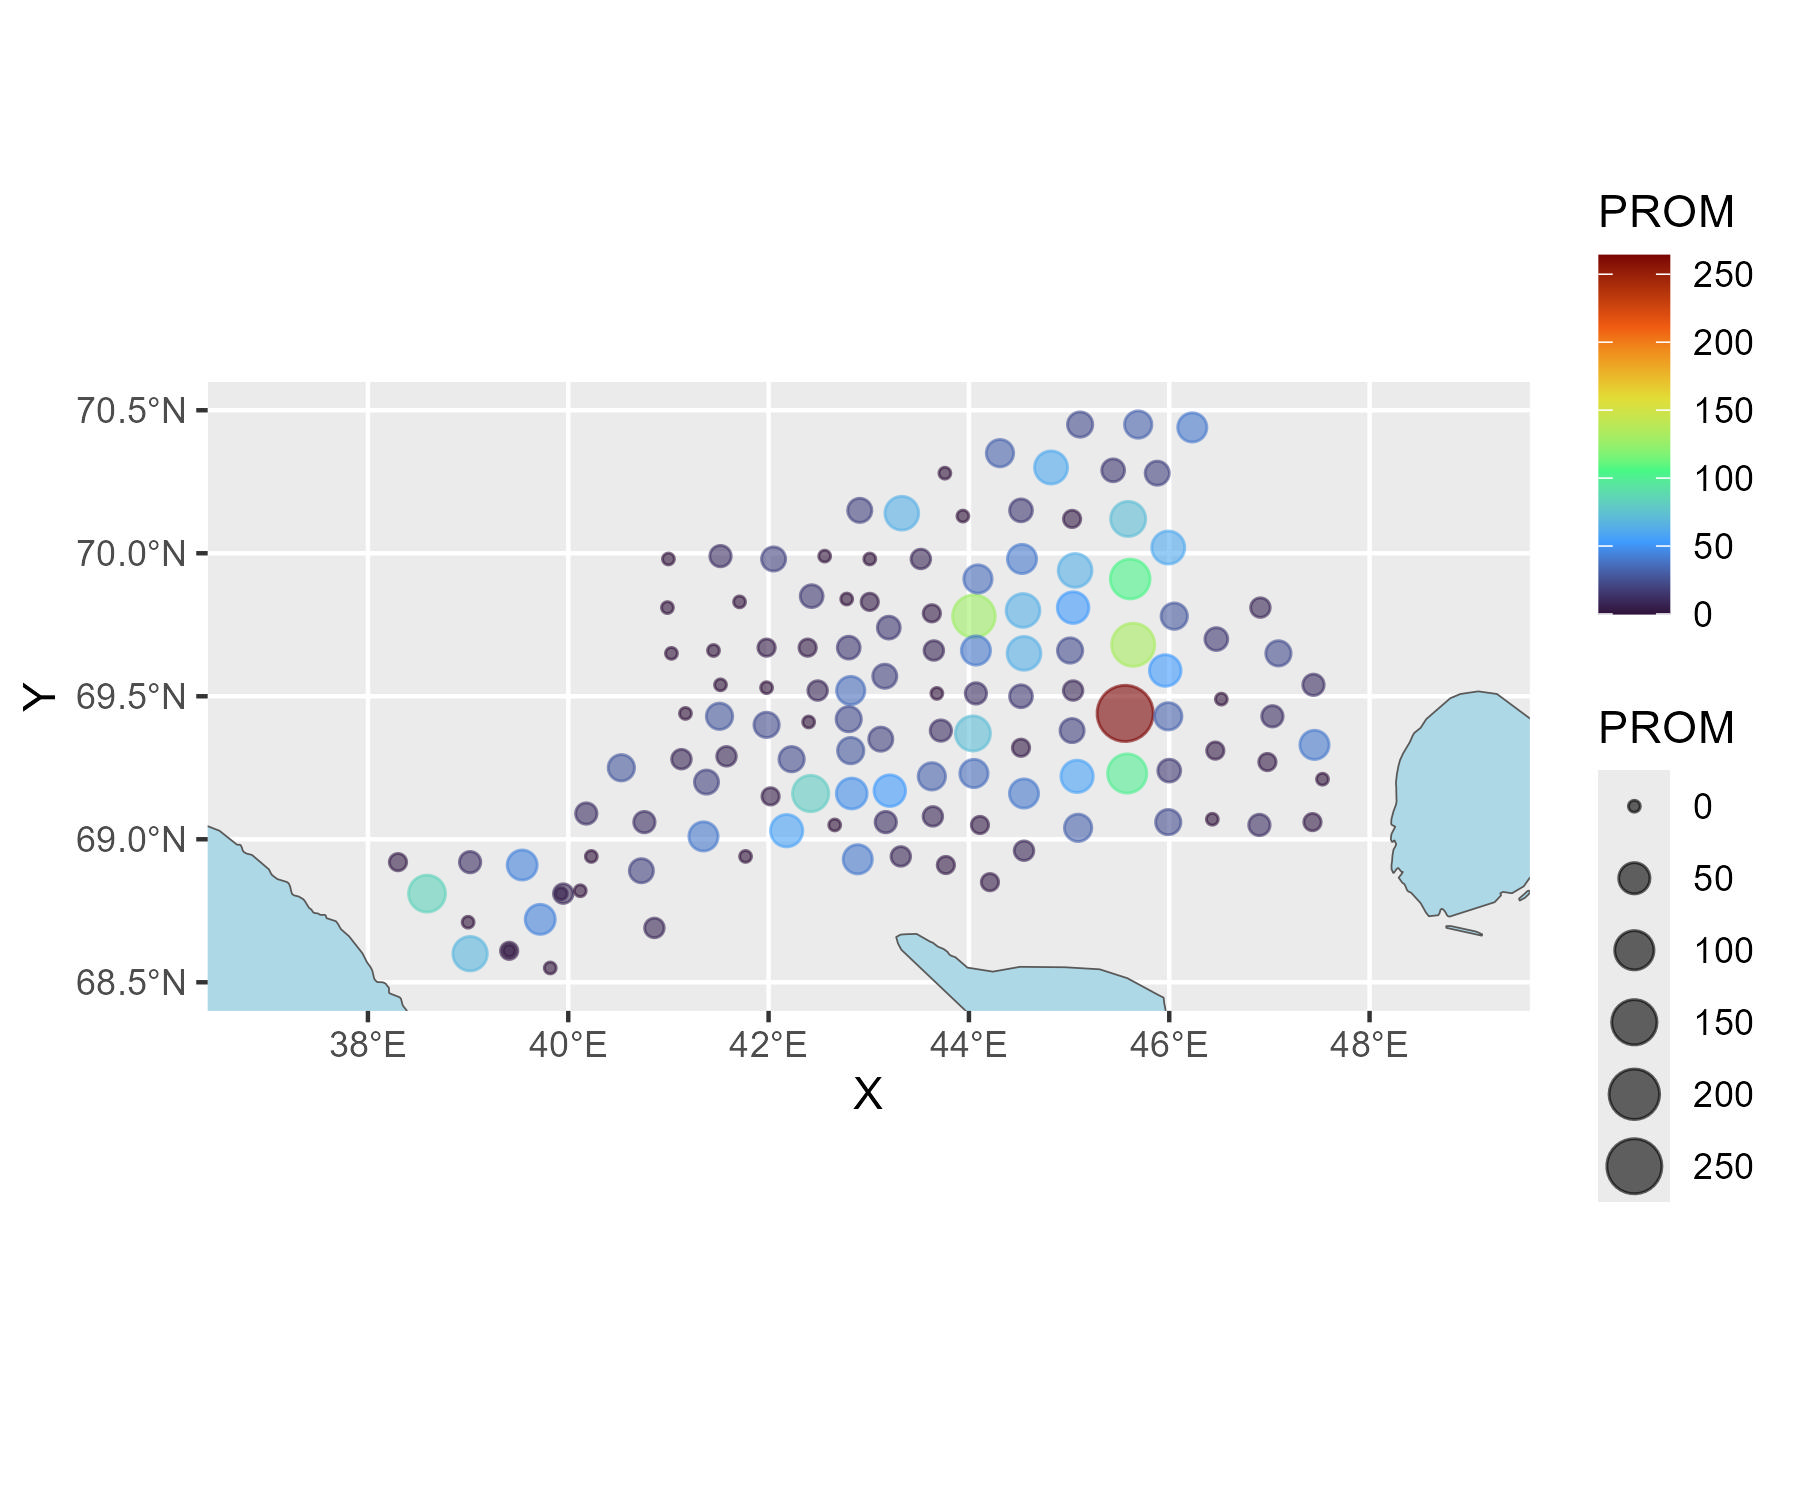
\includegraphics[width=0.7\linewidth,height=\textheight,keepaspectratio]{images/KARTOGRAPH2.jpg}

}

\caption{Рис. 2.: Пример карты распределения уловов в съемке с береговой
линией}

\end{figure}%

\begin{Shaded}
\begin{Highlighting}[]
\CommentTok{\# Очистка окружения и установка рабочей директории}
\FunctionTok{rm}\NormalTok{(}\AttributeTok{list =} \FunctionTok{ls}\NormalTok{())  }\CommentTok{\# Удаление всех объектов из глобального окружения}
\FunctionTok{setwd}\NormalTok{(}\StringTok{"C:/COURSES/KARTOGRAPH/"}\NormalTok{)  }\CommentTok{\# Установка рабочей директории}

\CommentTok{\# Загрузка необходимых библиотек}
\FunctionTok{library}\NormalTok{(rnaturalearth)  }\CommentTok{\# Для получения векторных карт мира}
\FunctionTok{library}\NormalTok{(tidyverse)      }\CommentTok{\# Коллекция пакетов для работы с данными}
\FunctionTok{library}\NormalTok{(sf)             }\CommentTok{\# Пространственный анализ}

\DocumentationTok{\#\#\#\#\#\#\# ЗАГРУЗКА ДАННЫХ И ПОДГОТОВКА ПРОСТРАНСТВЕННЫХ ОБЪЕКТОВ \#\#\#\#\#\#\#\#\#\#\#\#\#\#\#\#}

\CommentTok{\# Чтение и фильтрация данных}
\NormalTok{DATA }\OtherTok{\textless{}{-}}\NormalTok{ readxl}\SpecialCharTok{::}\FunctionTok{read\_excel}\NormalTok{(}\StringTok{"KARTOGRAPHIC.xlsx"}\NormalTok{, }\AttributeTok{sheet =} \StringTok{"SURVEY"}\NormalTok{) }\SpecialCharTok{\%\textgreater{}\%} 
  \FunctionTok{filter}\NormalTok{(YEAR }\SpecialCharTok{==} \DecValTok{2023}\NormalTok{, SURV }\SpecialCharTok{==} \StringTok{"CRAB"}\NormalTok{)  }\CommentTok{\# Фильтр данных за 2023 год по типу съемки}

\CommentTok{\# Получение границ России}
\NormalTok{russia }\OtherTok{\textless{}{-}} \FunctionTok{ne\_countries}\NormalTok{(}\AttributeTok{scale =} \DecValTok{10}\NormalTok{, }\AttributeTok{country =} \StringTok{"Russia"}\NormalTok{)  }\CommentTok{\# Загрузка векторных границ (масштаб 1:10м)}

\CommentTok{\# Установка границ отображаемой области (долгота/широта)}
\NormalTok{xmin}\OtherTok{=}\DecValTok{37}  \CommentTok{\# Западная граница}
\NormalTok{xmax}\OtherTok{=}\DecValTok{49}  \CommentTok{\# Восточная граница}
\NormalTok{ymin}\OtherTok{=}\FloatTok{68.5} \CommentTok{\# Южная граница}
\NormalTok{ymax}\OtherTok{=}\FloatTok{70.5} \CommentTok{\# Северная граница}

\CommentTok{\# Построение карты}
\FunctionTok{ggplot}\NormalTok{() }\SpecialCharTok{+}
  \CommentTok{\# Базовая карта России}
  \FunctionTok{geom\_sf}\NormalTok{(}\AttributeTok{data =}\NormalTok{ russia, }\AttributeTok{fill =} \StringTok{"lightblue"}\NormalTok{) }\SpecialCharTok{+} 
  \CommentTok{\# Ограничение области отображения}
  \FunctionTok{coord\_sf}\NormalTok{(}\AttributeTok{xlim =} \FunctionTok{c}\NormalTok{(xmin, xmax), }\AttributeTok{ylim =} \FunctionTok{c}\NormalTok{(ymin, ymax)) }\SpecialCharTok{+}
  \CommentTok{\# Точки наблюдений с размером и цветом по переменной PROM}
  \FunctionTok{geom\_point}\NormalTok{(}\FunctionTok{aes}\NormalTok{(}\AttributeTok{x =}\NormalTok{ X, }\AttributeTok{y =}\NormalTok{ Y, }\AttributeTok{size =}\NormalTok{ PROM, }\AttributeTok{color =}\NormalTok{ PROM),}
             \AttributeTok{data =}\NormalTok{ DATA, }\AttributeTok{alpha =} \FloatTok{0.6}\NormalTok{) }\SpecialCharTok{+}
  \CommentTok{\# Цветовая шкала (viridis, вариант H)}
  \FunctionTok{scale\_color\_viridis\_c}\NormalTok{(}\AttributeTok{option =} \StringTok{"H"}\NormalTok{)}
\end{Highlighting}
\end{Shaded}

\section{Карта распределения уловов, включая
нулевые}\label{ux43aux430ux440ux442ux430-ux440ux430ux441ux43fux440ux435ux434ux435ux43bux435ux43dux438ux44f-ux443ux43bux43eux432ux43eux432-ux432ux43aux43bux44eux447ux430ux44f-ux43dux443ux43bux435ux432ux44bux435}

\begin{figure}[H]

{\centering 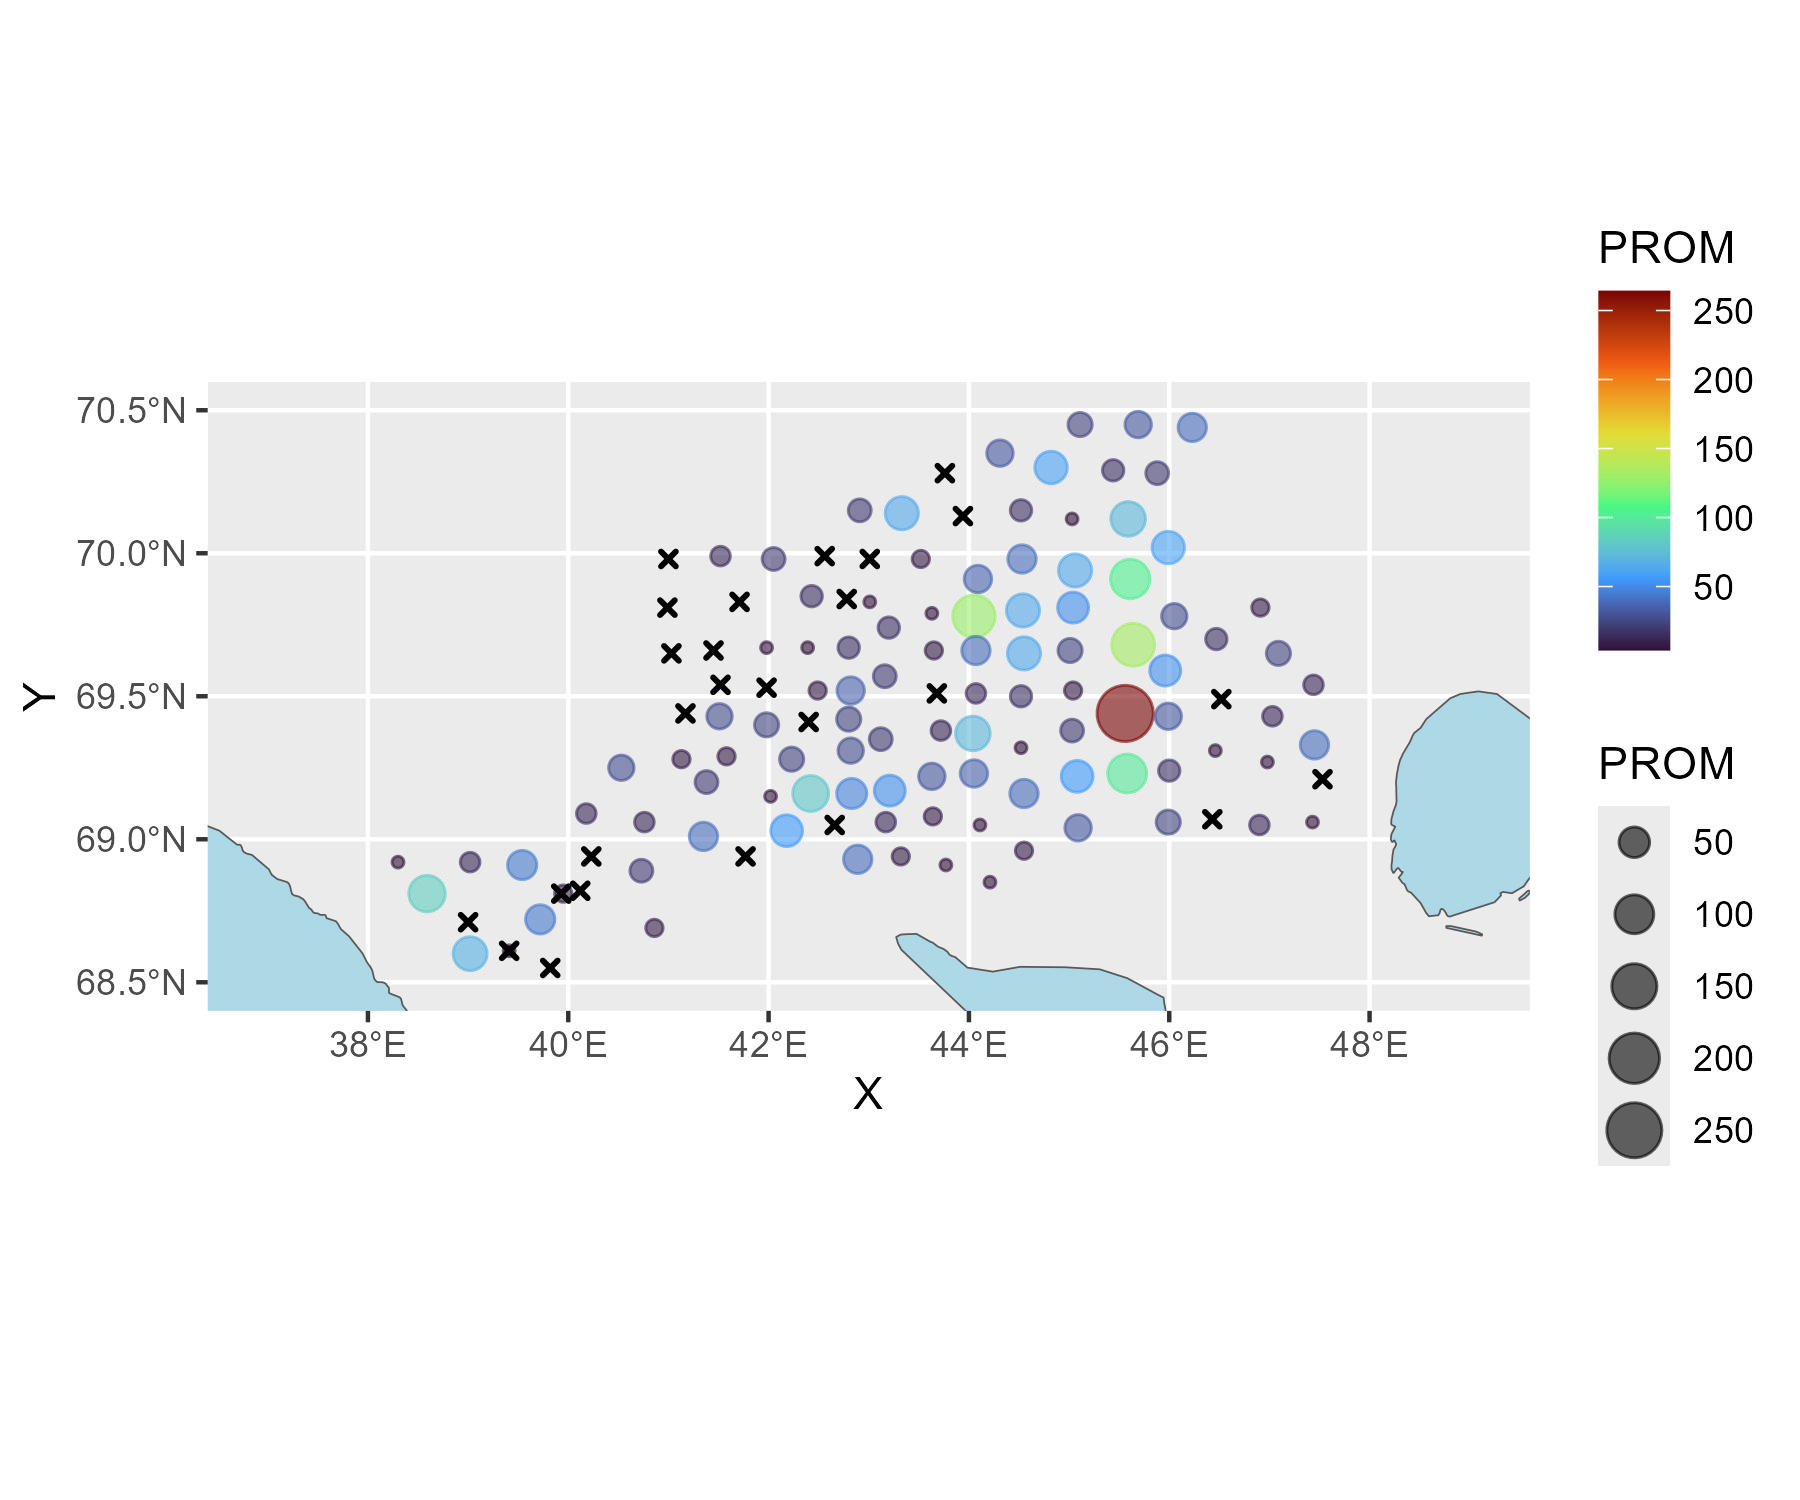
\includegraphics[width=0.7\linewidth,height=\textheight,keepaspectratio]{images/KARTOGRAPH3.jpg}

}

\caption{Рис. 3.: Карта распределения уловов, включая нулевые}

\end{figure}%

\begin{Shaded}
\begin{Highlighting}[]
\CommentTok{\# Очистка окружения и установка рабочей директории}
\FunctionTok{rm}\NormalTok{(}\AttributeTok{list =} \FunctionTok{ls}\NormalTok{())  }\CommentTok{\# Удаление всех объектов из глобального окружения}
\FunctionTok{setwd}\NormalTok{(}\StringTok{"C:/COURSES/KARTOGRAPH/"}\NormalTok{)  }\CommentTok{\# Установка рабочей директории}

\CommentTok{\# Загрузка необходимых библиотек}
\FunctionTok{library}\NormalTok{(rnaturalearth)  }\CommentTok{\# Для получения векторных карт мира}
\FunctionTok{library}\NormalTok{(tidyverse)      }\CommentTok{\# Коллекция пакетов для работы с данными}
\FunctionTok{library}\NormalTok{(sf)             }\CommentTok{\# Пространственный анализ}

\DocumentationTok{\#\#\#\#\#\#\# ЗАГРУЗКА ДАННЫХ И ПОДГОТОВКА ПРОСТРАНСТВЕННЫХ ОБЪЕКТОВ \#\#\#\#\#\#\#\#\#\#\#\#\#\#\#\#}

\CommentTok{\# Чтение и фильтрация данных}
\NormalTok{DATA }\OtherTok{\textless{}{-}}\NormalTok{ readxl}\SpecialCharTok{::}\FunctionTok{read\_excel}\NormalTok{(}\StringTok{"KARTOGRAPHIC.xlsx"}\NormalTok{, }\AttributeTok{sheet =} \StringTok{"SURVEY"}\NormalTok{) }\SpecialCharTok{\%\textgreater{}\%} 
  \FunctionTok{filter}\NormalTok{(YEAR }\SpecialCharTok{==} \DecValTok{2023}\NormalTok{, SURV }\SpecialCharTok{==} \StringTok{"CRAB"}\NormalTok{)  }\CommentTok{\# Фильтр данных за 2023 год по типу съемки}

\CommentTok{\# Получение границ России}
\NormalTok{russia }\OtherTok{\textless{}{-}} \FunctionTok{ne\_countries}\NormalTok{(}\AttributeTok{scale =} \DecValTok{10}\NormalTok{, }\AttributeTok{country =} \StringTok{"Russia"}\NormalTok{)  }\CommentTok{\# Загрузка векторных границ (масштаб 1:10м)}

\CommentTok{\# Установка границ отображаемой области (долгота/широта)}
\NormalTok{xmin}\OtherTok{=}\DecValTok{37}  \CommentTok{\# Западная граница}
\NormalTok{xmax}\OtherTok{=}\DecValTok{49}  \CommentTok{\# Восточная граница}
\NormalTok{ymin}\OtherTok{=}\FloatTok{68.5} \CommentTok{\# Южная граница}
\NormalTok{ymax}\OtherTok{=}\FloatTok{70.5} \CommentTok{\# Северная граница}

\CommentTok{\# Построение карты}
\FunctionTok{ggplot}\NormalTok{() }\SpecialCharTok{+}
  \CommentTok{\# Базовая карта России}
  \FunctionTok{geom\_sf}\NormalTok{(}\AttributeTok{data =}\NormalTok{ russia, }\AttributeTok{fill =} \StringTok{"lightblue"}\NormalTok{) }\SpecialCharTok{+} 
  \CommentTok{\# Ограничение области отображения}
  \FunctionTok{coord\_sf}\NormalTok{(}\AttributeTok{xlim =} \FunctionTok{c}\NormalTok{(xmin, xmax), }\AttributeTok{ylim =} \FunctionTok{c}\NormalTok{(ymin, ymax)) }\SpecialCharTok{+}
  \CommentTok{\# Точки наблюдений с размером и цветом по переменной PROM (ненулевые уловы)}
  \FunctionTok{geom\_point}\NormalTok{(}\FunctionTok{aes}\NormalTok{(}\AttributeTok{x =}\NormalTok{ X, }\AttributeTok{y =}\NormalTok{ Y, }\AttributeTok{size =}\NormalTok{ PROM, }\AttributeTok{color =}\NormalTok{ PROM),}
             \AttributeTok{data =} \FunctionTok{filter}\NormalTok{(DATA, PROM }\SpecialCharTok{\textgreater{}} \DecValTok{0}\NormalTok{), }\AttributeTok{alpha =} \FloatTok{0.6}\NormalTok{) }\SpecialCharTok{+}
  \CommentTok{\# Точки для нулевых уловов (крестики)}
  \FunctionTok{geom\_point}\NormalTok{(}\FunctionTok{aes}\NormalTok{(}\AttributeTok{x =}\NormalTok{ X, }\AttributeTok{y =}\NormalTok{ Y),}
             \AttributeTok{data =} \FunctionTok{filter}\NormalTok{(DATA, PROM }\SpecialCharTok{==} \DecValTok{0}\NormalTok{),}
             \AttributeTok{shape =} \DecValTok{4}\NormalTok{, }\AttributeTok{size =} \DecValTok{1}\NormalTok{, }\AttributeTok{stroke =} \DecValTok{1}\NormalTok{, }\AttributeTok{color =} \StringTok{"black"}\NormalTok{) }\SpecialCharTok{+}
  \CommentTok{\# Цветовая шкала (viridis, вариант H)}
  \FunctionTok{scale\_color\_viridis\_c}\NormalTok{(}\AttributeTok{option =} \StringTok{"H"}\NormalTok{)}
\end{Highlighting}
\end{Shaded}

\section{Карта распределения уловов, распределенных по
квартилям}\label{ux43aux430ux440ux442ux430-ux440ux430ux441ux43fux440ux435ux434ux435ux43bux435ux43dux438ux44f-ux443ux43bux43eux432ux43eux432-ux440ux430ux441ux43fux440ux435ux434ux435ux43bux435ux43dux43dux44bux445-ux43fux43e-ux43aux432ux430ux440ux442ux438ux43bux44fux43c}

\begin{figure}[H]

{\centering 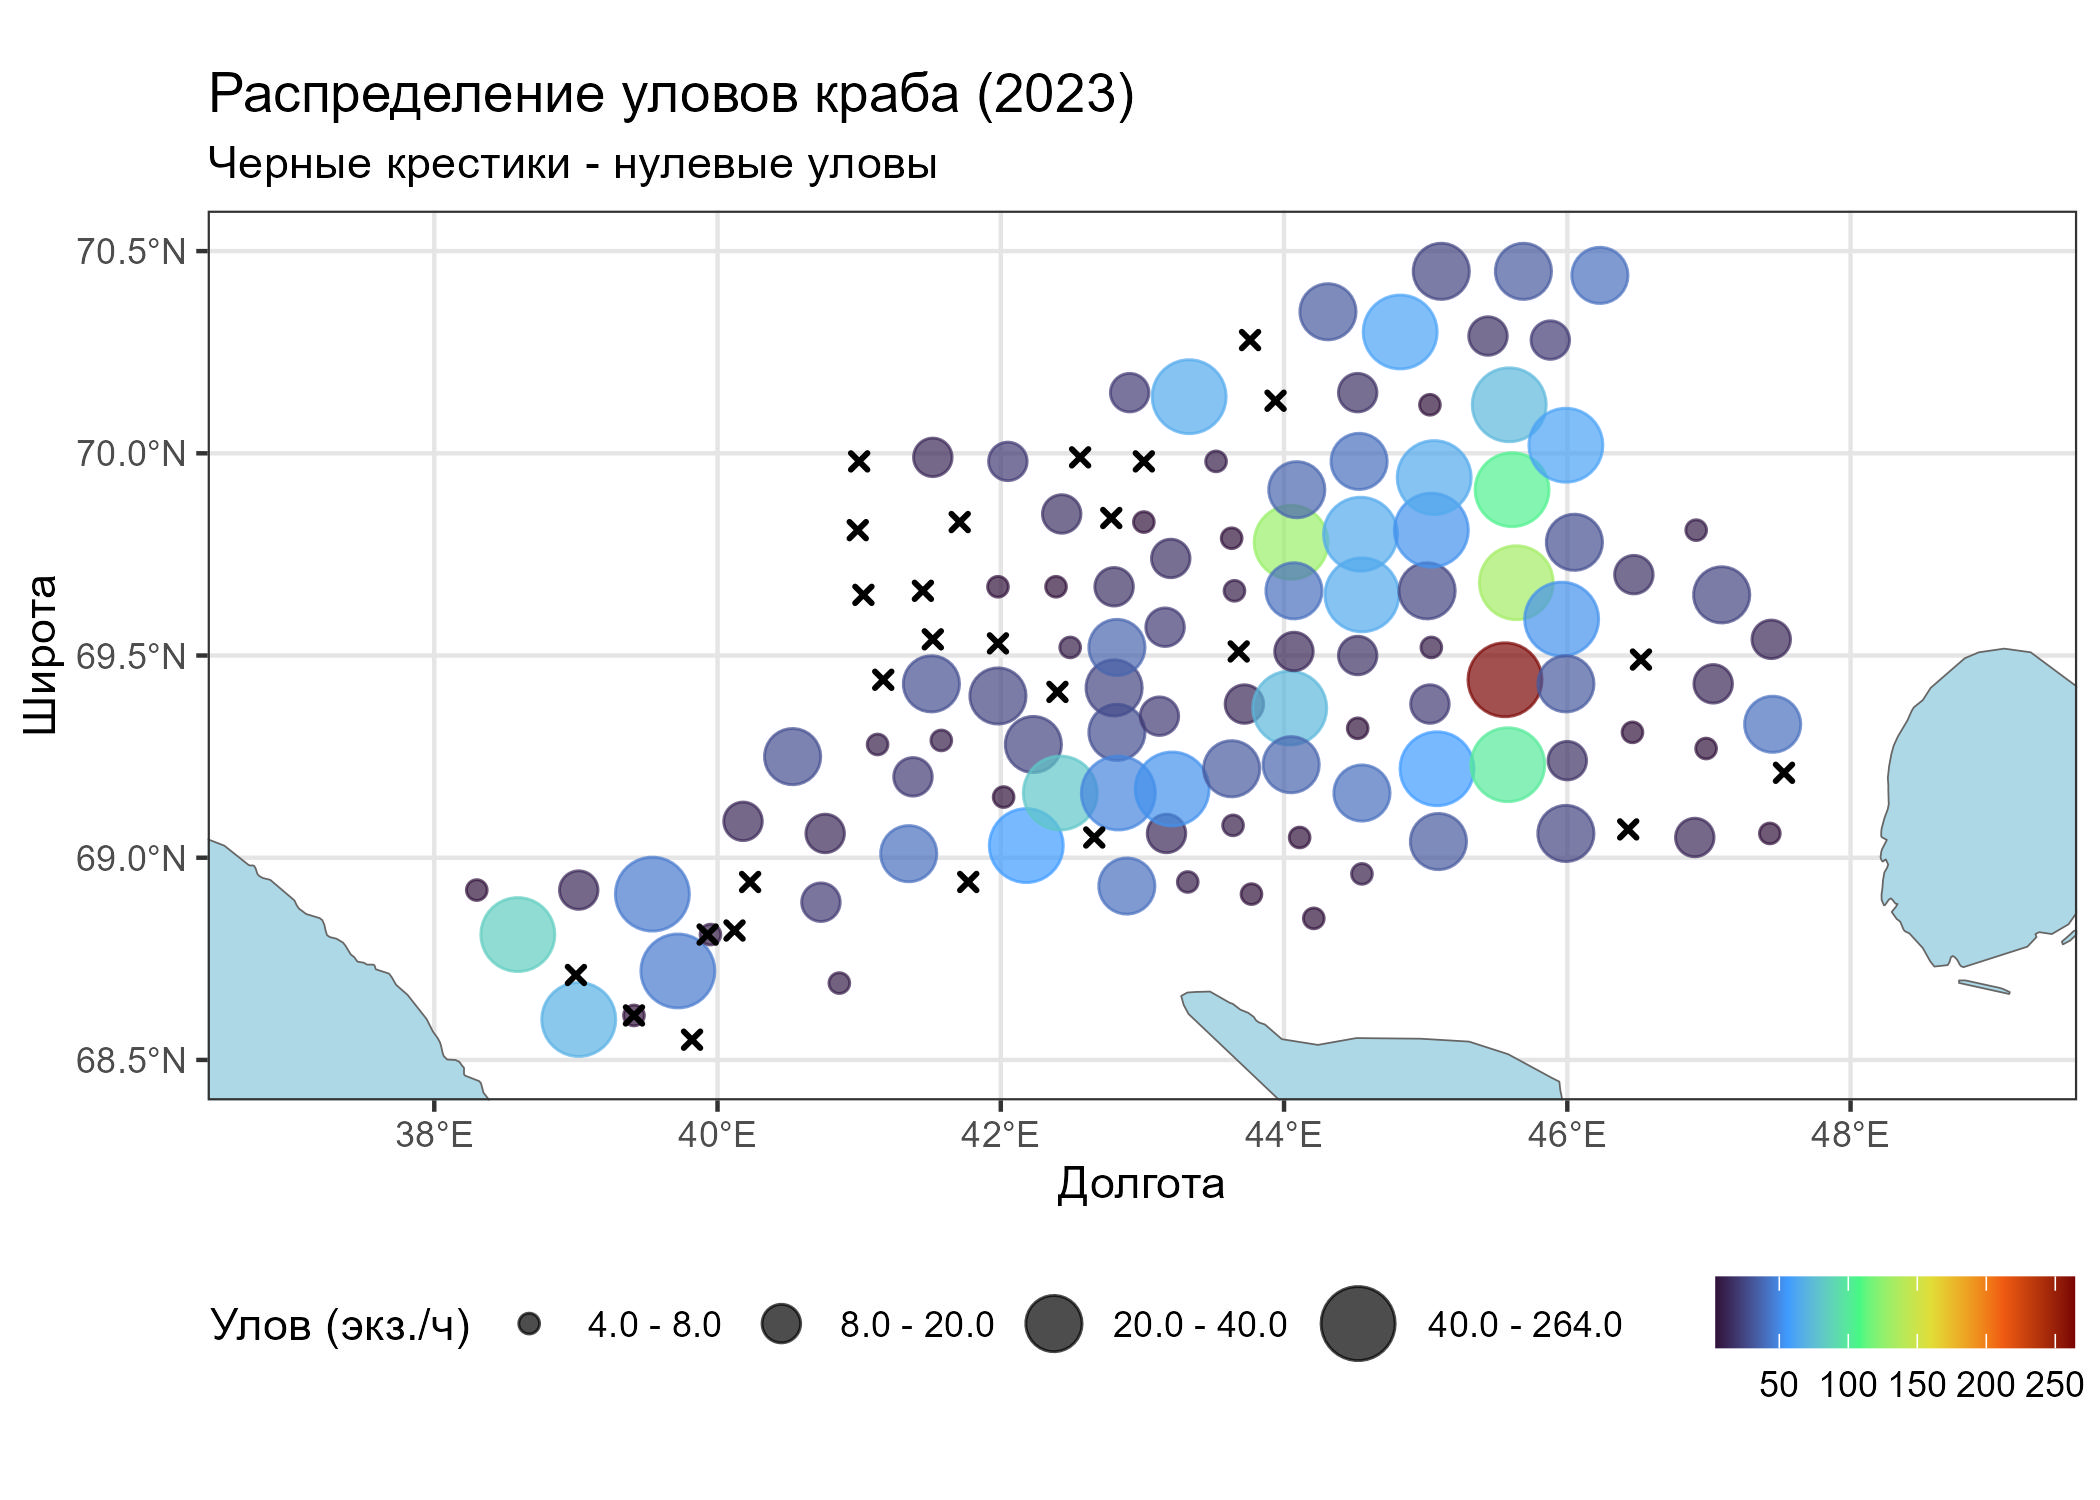
\includegraphics[width=0.7\linewidth,height=\textheight,keepaspectratio]{images/KARTOGRAPH4.jpg}

}

\caption{Рис. 4.: Карта распределения уловов, распределенных по
квартилям}

\end{figure}%

\begin{Shaded}
\begin{Highlighting}[]
\CommentTok{\# Очистка окружения и установка рабочей директории}
\FunctionTok{rm}\NormalTok{(}\AttributeTok{list =} \FunctionTok{ls}\NormalTok{())}
\FunctionTok{setwd}\NormalTok{(}\StringTok{"C:/COURSES/KARTOGRAPH/"}\NormalTok{)}

\CommentTok{\# Загрузка необходимых библиотек}
\FunctionTok{library}\NormalTok{(rnaturalearth)}
\FunctionTok{library}\NormalTok{(tidyverse)}
\FunctionTok{library}\NormalTok{(sf)}

\DocumentationTok{\#\#\#\#\#\#\# ЗАГРУЗКА ДАННЫХ И ПОДГОТОВКА ПРОСТРАНСТВЕННЫХ ОБЪЕКТОВ \#\#\#\#\#\#\#\#\#\#\#\#\#\#\#\#}

\CommentTok{\# Чтение и фильтрация данных}
\NormalTok{DATA }\OtherTok{\textless{}{-}}\NormalTok{ readxl}\SpecialCharTok{::}\FunctionTok{read\_excel}\NormalTok{(}\StringTok{"KARTOGRAPHIC.xlsx"}\NormalTok{, }\AttributeTok{sheet =} \StringTok{"SURVEY"}\NormalTok{) }\SpecialCharTok{\%\textgreater{}\%} 
  \FunctionTok{filter}\NormalTok{(YEAR }\SpecialCharTok{==} \DecValTok{2023}\NormalTok{, SURV }\SpecialCharTok{==} \StringTok{"CRAB"}\NormalTok{)}

\CommentTok{\# Получение границ России}
\NormalTok{russia }\OtherTok{\textless{}{-}} \FunctionTok{ne\_countries}\NormalTok{(}\AttributeTok{scale =} \DecValTok{10}\NormalTok{, }\AttributeTok{country =} \StringTok{"Russia"}\NormalTok{) }\SpecialCharTok{\%\textgreater{}\%} 
  \FunctionTok{st\_as\_sf}\NormalTok{()}

\CommentTok{\# Установка границ отображаемой области}
\NormalTok{xmin}\OtherTok{=}\DecValTok{37}\NormalTok{; xmax}\OtherTok{=}\DecValTok{49}\NormalTok{; ymin}\OtherTok{=}\FloatTok{68.5}\NormalTok{; ymax}\OtherTok{=}\FloatTok{70.5}

\DocumentationTok{\#\#\#\#\#\#\# ПОДГОТОВКА ДАННЫХ ДЛЯ ВИЗУАЛИЗАЦИИ \#\#\#\#\#\#\#\#\#\#\#\#\#\#\#\#}
\CommentTok{\# Вычисляем квартили отдельно}
\NormalTok{quantiles }\OtherTok{\textless{}{-}} \FunctionTok{quantile}\NormalTok{(DATA}\SpecialCharTok{$}\NormalTok{PROM[DATA}\SpecialCharTok{$}\NormalTok{PROM }\SpecialCharTok{\textgreater{}} \DecValTok{0}\NormalTok{], }\AttributeTok{probs =} \FunctionTok{seq}\NormalTok{(}\DecValTok{0}\NormalTok{, }\DecValTok{1}\NormalTok{, }\FloatTok{0.25}\NormalTok{))}

\CommentTok{\# Создаем 4 категории с реальными диапазонами значений}
\NormalTok{nonzero\_data }\OtherTok{\textless{}{-}}\NormalTok{ DATA }\SpecialCharTok{\%\textgreater{}\%} 
  \FunctionTok{filter}\NormalTok{(PROM }\SpecialCharTok{\textgreater{}} \DecValTok{0}\NormalTok{) }\SpecialCharTok{\%\textgreater{}\%}
  \FunctionTok{mutate}\NormalTok{(}
    \AttributeTok{PROM\_cat =} \FunctionTok{cut}\NormalTok{(}
\NormalTok{      PROM,}
      \AttributeTok{breaks =}\NormalTok{ quantiles,}
      \AttributeTok{include.lowest =} \ConstantTok{TRUE}\NormalTok{,}
      \AttributeTok{labels =} \FunctionTok{c}\NormalTok{(}
        \FunctionTok{sprintf}\NormalTok{(}\StringTok{"\%.1f {-} \%.1f"}\NormalTok{, quantiles[}\DecValTok{1}\NormalTok{], quantiles[}\DecValTok{2}\NormalTok{]),}
        \FunctionTok{sprintf}\NormalTok{(}\StringTok{"\%.1f {-} \%.1f"}\NormalTok{, quantiles[}\DecValTok{2}\NormalTok{], quantiles[}\DecValTok{3}\NormalTok{]),}
        \FunctionTok{sprintf}\NormalTok{(}\StringTok{"\%.1f {-} \%.1f"}\NormalTok{, quantiles[}\DecValTok{3}\NormalTok{], quantiles[}\DecValTok{4}\NormalTok{]),}
        \FunctionTok{sprintf}\NormalTok{(}\StringTok{"\%.1f {-} \%.1f"}\NormalTok{, quantiles[}\DecValTok{4}\NormalTok{], quantiles[}\DecValTok{5}\NormalTok{])}
\NormalTok{      )}
\NormalTok{    )}
\NormalTok{  )}

\CommentTok{\# Построение карты}
\FunctionTok{ggplot}\NormalTok{() }\SpecialCharTok{+}
  \CommentTok{\# Базовая карта России}
  \FunctionTok{geom\_sf}\NormalTok{(}\AttributeTok{data =}\NormalTok{ russia, }\AttributeTok{fill =} \StringTok{"lightblue"}\NormalTok{, }\AttributeTok{color =} \StringTok{"gray40"}\NormalTok{) }\SpecialCharTok{+} 
  \CommentTok{\# Ограничение области отображения}
  \FunctionTok{coord\_sf}\NormalTok{(}\AttributeTok{xlim =} \FunctionTok{c}\NormalTok{(xmin, xmax), }\AttributeTok{ylim =} \FunctionTok{c}\NormalTok{(ymin, ymax)) }\SpecialCharTok{+}
  \CommentTok{\# Точки наблюдений с категориальным размером}
  \FunctionTok{geom\_point}\NormalTok{(}
    \AttributeTok{data =}\NormalTok{ nonzero\_data,}
    \FunctionTok{aes}\NormalTok{(}\AttributeTok{x =}\NormalTok{ X, }\AttributeTok{y =}\NormalTok{ Y, }\AttributeTok{size =}\NormalTok{ PROM\_cat, }\AttributeTok{color =}\NormalTok{ PROM),}
    \AttributeTok{alpha =} \FloatTok{0.7}
\NormalTok{  ) }\SpecialCharTok{+}
  \CommentTok{\# Точки для нулевых уловов (крестики)}
  \FunctionTok{geom\_point}\NormalTok{(}
    \AttributeTok{data =} \FunctionTok{filter}\NormalTok{(DATA, PROM }\SpecialCharTok{==} \DecValTok{0}\NormalTok{),}
    \FunctionTok{aes}\NormalTok{(}\AttributeTok{x =}\NormalTok{ X, }\AttributeTok{y =}\NormalTok{ Y),}
    \AttributeTok{shape =} \DecValTok{4}\NormalTok{, }\AttributeTok{size =} \FloatTok{1.2}\NormalTok{, }\AttributeTok{stroke =} \DecValTok{1}\NormalTok{, }\AttributeTok{color =} \StringTok{"black"}
\NormalTok{  ) }\SpecialCharTok{+}
  \CommentTok{\# Цветовая шкала (непрерывная)}
  \FunctionTok{scale\_color\_viridis\_c}\NormalTok{(}\AttributeTok{option =} \StringTok{"H"}\NormalTok{, }\AttributeTok{name =} \ConstantTok{NULL}\NormalTok{) }\SpecialCharTok{+}
  \CommentTok{\# Ручная настройка размеров для категорий}
  \FunctionTok{scale\_size\_manual}\NormalTok{(}
    \AttributeTok{name =} \StringTok{"Улов (экз./ч)"}\NormalTok{,}
    \AttributeTok{values =} \FunctionTok{c}\NormalTok{(}\DecValTok{2}\NormalTok{, }\DecValTok{4}\NormalTok{, }\DecValTok{6}\NormalTok{, }\DecValTok{8}\NormalTok{),  }\CommentTok{\# Размеры точек для категорий}
    \AttributeTok{drop =} \ConstantTok{FALSE}
\NormalTok{  ) }\SpecialCharTok{+}
  \CommentTok{\# Настройки темы}
  \FunctionTok{theme\_bw}\NormalTok{() }\SpecialCharTok{+}
  \FunctionTok{labs}\NormalTok{(}
    \AttributeTok{title =} \StringTok{"Распределение уловов краба (2023)"}\NormalTok{,}
    \AttributeTok{subtitle =} \StringTok{"Черные крестики {-} нулевые уловы"}\NormalTok{,}
    \AttributeTok{x =} \StringTok{"Долгота"}\NormalTok{, }
    \AttributeTok{y =} \StringTok{"Широта"}
\NormalTok{  ) }\SpecialCharTok{+}
  \FunctionTok{theme}\NormalTok{(}
    \AttributeTok{panel.grid =} \FunctionTok{element\_line}\NormalTok{(}\AttributeTok{color =} \StringTok{"gray90"}\NormalTok{),}
    \AttributeTok{legend.position =} \StringTok{"bottom"}
\NormalTok{  )}
\end{Highlighting}
\end{Shaded}

\section{Карта распределения уловов по
фасеткам}\label{ux43aux430ux440ux442ux430-ux440ux430ux441ux43fux440ux435ux434ux435ux43bux435ux43dux438ux44f-ux443ux43bux43eux432ux43eux432-ux43fux43e-ux444ux430ux441ux435ux442ux43aux430ux43c}

\begin{figure}[H]

{\centering 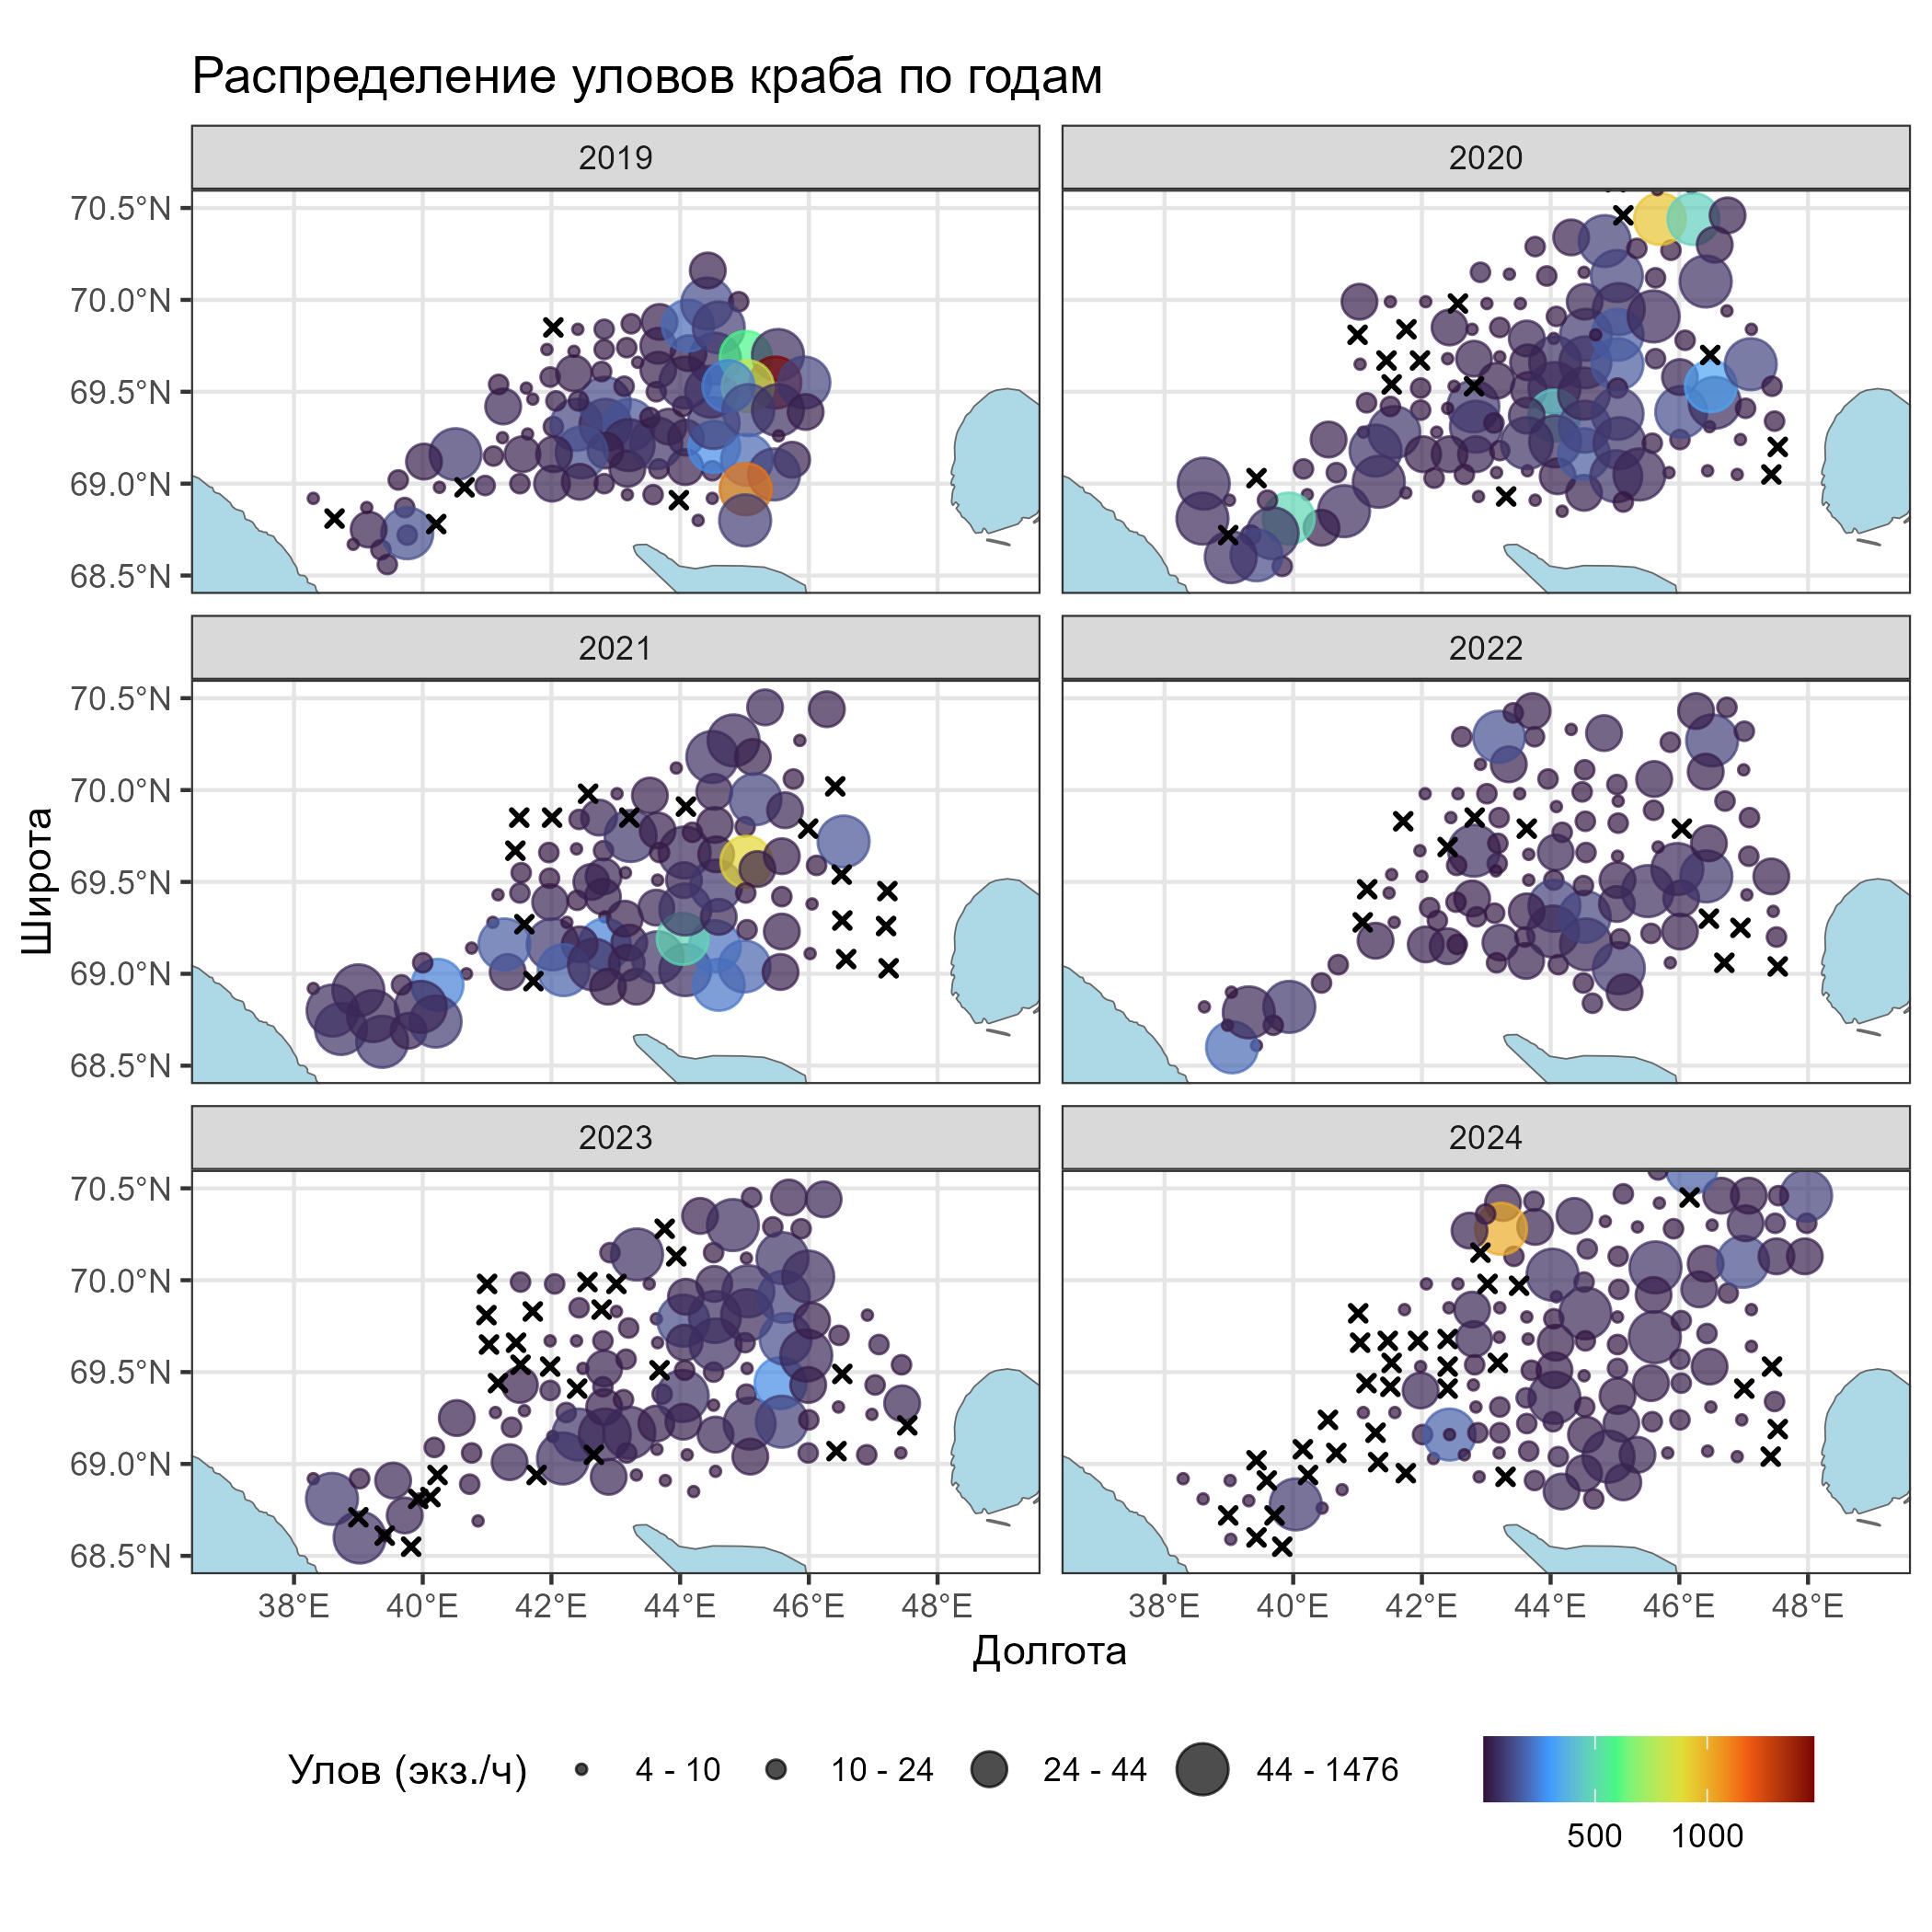
\includegraphics[width=0.8\linewidth,height=\textheight,keepaspectratio]{images/KARTOGRAPH5.jpg}

}

\caption{Рис. 5.: Карта распределения уловов по фасеткам}

\end{figure}%

\begin{Shaded}
\begin{Highlighting}[]
\CommentTok{\# Очистка окружения и установка рабочей директории}
\FunctionTok{rm}\NormalTok{(}\AttributeTok{list =} \FunctionTok{ls}\NormalTok{())}
\FunctionTok{setwd}\NormalTok{(}\StringTok{"C:/COURSES/KARTOGRAPH/"}\NormalTok{)}

\CommentTok{\# Установка и подключение библиотек (если не установлено — раскомментируй)}
\CommentTok{\# install.packages(c("rnaturalearth", "tidyverse", "sf", "readxl", "viridis"))}
\FunctionTok{library}\NormalTok{(rnaturalearth)}
\FunctionTok{library}\NormalTok{(tidyverse)}
\FunctionTok{library}\NormalTok{(sf)}
\FunctionTok{library}\NormalTok{(readxl)}
\FunctionTok{library}\NormalTok{(viridis)}

\DocumentationTok{\#\#\#\#\#\#\# ЗАГРУЗКА ДАННЫХ И ПОДГОТОВКА ПРОСТРАНСТВЕННЫХ ОБЪЕКТОВ \#\#\#\#\#\#\#\#\#\#\#\#\#\#\#\#}

\CommentTok{\# Чтение и фильтрация данных (убираем фильтр по году, чтобы работать со всеми годами)}
\NormalTok{DATA }\OtherTok{\textless{}{-}}\NormalTok{ readxl}\SpecialCharTok{::}\FunctionTok{read\_excel}\NormalTok{(}\StringTok{"KARTOGRAPHIC.xlsx"}\NormalTok{, }\AttributeTok{sheet =} \StringTok{"SURVEY"}\NormalTok{) }\SpecialCharTok{\%\textgreater{}\%} 
  \FunctionTok{filter}\NormalTok{(SURV }\SpecialCharTok{==} \StringTok{"CRAB"}\NormalTok{)}

\CommentTok{\# Получение границ России}
\NormalTok{russia }\OtherTok{\textless{}{-}} \FunctionTok{ne\_countries}\NormalTok{(}\AttributeTok{scale =} \DecValTok{10}\NormalTok{, }\AttributeTok{country =} \StringTok{"Russia"}\NormalTok{) }\SpecialCharTok{\%\textgreater{}\%} 
  \FunctionTok{st\_as\_sf}\NormalTok{()}

\CommentTok{\# Установка границ отображаемой области}
\NormalTok{xmin }\OtherTok{\textless{}{-}} \DecValTok{37}\NormalTok{; xmax }\OtherTok{\textless{}{-}} \DecValTok{49}
\NormalTok{ymin }\OtherTok{\textless{}{-}} \FloatTok{68.5}\NormalTok{; ymax }\OtherTok{\textless{}{-}} \FloatTok{70.5}

\CommentTok{\# Вычисляем общие квартили для всех лет (чтобы категории были сопоставимыми)}
\NormalTok{quantiles }\OtherTok{\textless{}{-}} \FunctionTok{quantile}\NormalTok{(DATA}\SpecialCharTok{$}\NormalTok{PROM[DATA}\SpecialCharTok{$}\NormalTok{PROM }\SpecialCharTok{\textgreater{}} \DecValTok{0}\NormalTok{], }\AttributeTok{probs =} \FunctionTok{seq}\NormalTok{(}\DecValTok{0}\NormalTok{, }\DecValTok{1}\NormalTok{, }\FloatTok{0.25}\NormalTok{))}

\CommentTok{\# Создаем данные с ненулевыми уловами и категориями}
\NormalTok{nonzero\_data }\OtherTok{\textless{}{-}}\NormalTok{ DATA }\SpecialCharTok{\%\textgreater{}\%}
  \FunctionTok{filter}\NormalTok{(PROM }\SpecialCharTok{\textgreater{}} \DecValTok{0}\NormalTok{) }\SpecialCharTok{\%\textgreater{}\%}
  \FunctionTok{mutate}\NormalTok{(}
\AttributeTok{PROM\_cat =} \FunctionTok{cut}\NormalTok{(}
\NormalTok{  PROM,}
  \AttributeTok{breaks =} \FunctionTok{c}\NormalTok{(}\SpecialCharTok{{-}}\ConstantTok{Inf}\NormalTok{, quantiles[}\DecValTok{2}\SpecialCharTok{:}\DecValTok{4}\NormalTok{], }\ConstantTok{Inf}\NormalTok{),}
  \AttributeTok{include.lowest =} \ConstantTok{TRUE}\NormalTok{,}
  \AttributeTok{labels =} \FunctionTok{c}\NormalTok{(}
    \FunctionTok{sprintf}\NormalTok{(}\StringTok{"\%d {-} \%d"}\NormalTok{, }\FunctionTok{floor}\NormalTok{(quantiles[}\DecValTok{1}\NormalTok{]), }\FunctionTok{floor}\NormalTok{(quantiles[}\DecValTok{2}\NormalTok{])),}
    \FunctionTok{sprintf}\NormalTok{(}\StringTok{"\%d {-} \%d"}\NormalTok{, }\FunctionTok{floor}\NormalTok{(quantiles[}\DecValTok{2}\NormalTok{]), }\FunctionTok{floor}\NormalTok{(quantiles[}\DecValTok{3}\NormalTok{])),}
    \FunctionTok{sprintf}\NormalTok{(}\StringTok{"\%d {-} \%d"}\NormalTok{, }\FunctionTok{floor}\NormalTok{(quantiles[}\DecValTok{3}\NormalTok{]), }\FunctionTok{floor}\NormalTok{(quantiles[}\DecValTok{4}\NormalTok{])),}
    \FunctionTok{sprintf}\NormalTok{(}\StringTok{"\%d {-} \%d"}\NormalTok{, }\FunctionTok{floor}\NormalTok{(quantiles[}\DecValTok{4}\NormalTok{]), }\FunctionTok{floor}\NormalTok{(}\FunctionTok{max}\NormalTok{(DATA}\SpecialCharTok{$}\NormalTok{PROM)))}
\NormalTok{  )}
\NormalTok{)}
\NormalTok{  )}

\CommentTok{\# Отдельно выделяем точки с нулевым уловом}
\NormalTok{zero\_data }\OtherTok{\textless{}{-}}\NormalTok{ DATA }\SpecialCharTok{\%\textgreater{}\%} \FunctionTok{filter}\NormalTok{(PROM }\SpecialCharTok{==} \DecValTok{0}\NormalTok{)}

\DocumentationTok{\#\#\#\#\#\#\# ВИЗУАЛИЗАЦИЯ \#\#\#\#\#\#\#\#\#\#\#\#\#\#\#\#}

\CommentTok{\# Фасеточная карта по годам}
\FunctionTok{ggplot}\NormalTok{() }\SpecialCharTok{+}
  \CommentTok{\# Граница России}
  \FunctionTok{geom\_sf}\NormalTok{(}\AttributeTok{data =}\NormalTok{ russia, }\AttributeTok{fill =} \StringTok{"lightblue"}\NormalTok{, }\AttributeTok{color =} \StringTok{"gray40"}\NormalTok{) }\SpecialCharTok{+}
  
  \CommentTok{\# Ограничение области отображения}
  \FunctionTok{coord\_sf}\NormalTok{(}\AttributeTok{xlim =} \FunctionTok{c}\NormalTok{(xmin, xmax), }\AttributeTok{ylim =} \FunctionTok{c}\NormalTok{(ymin, ymax)) }\SpecialCharTok{+}
  
  \CommentTok{\# Точки с уловом}
  \FunctionTok{geom\_point}\NormalTok{(}
    \AttributeTok{data =}\NormalTok{ nonzero\_data,}
    \FunctionTok{aes}\NormalTok{(}\AttributeTok{x =}\NormalTok{ X, }\AttributeTok{y =}\NormalTok{ Y, }\AttributeTok{size =}\NormalTok{ PROM\_cat, }\AttributeTok{color =}\NormalTok{ PROM),}
    \AttributeTok{alpha =} \FloatTok{0.7}
\NormalTok{  ) }\SpecialCharTok{+}
  
  \CommentTok{\# Нулевые уловы — крестики}
  \FunctionTok{geom\_point}\NormalTok{(}
    \AttributeTok{data =}\NormalTok{ zero\_data,}
    \FunctionTok{aes}\NormalTok{(}\AttributeTok{x =}\NormalTok{ X, }\AttributeTok{y =}\NormalTok{ Y),}
    \AttributeTok{shape =} \DecValTok{4}\NormalTok{, }\AttributeTok{size =} \FloatTok{1.2}\NormalTok{, }\AttributeTok{stroke =} \DecValTok{1}\NormalTok{, }\AttributeTok{color =} \StringTok{"black"}
\NormalTok{  ) }\SpecialCharTok{+}
  
  \CommentTok{\# Цветовая шкала}
  \FunctionTok{scale\_color\_viridis\_c}\NormalTok{(}\AttributeTok{option =} \StringTok{"H"}\NormalTok{, }\AttributeTok{name =} \ConstantTok{NULL}\NormalTok{) }\SpecialCharTok{+}
  
  \CommentTok{\# Настройка размеров точек по категориям}
  \FunctionTok{scale\_size\_manual}\NormalTok{(}
    \AttributeTok{name =} \StringTok{"Улов (экз./ч)"}\NormalTok{,}
    \AttributeTok{values =} \FunctionTok{c}\NormalTok{(}\DecValTok{1}\NormalTok{, }\DecValTok{2}\NormalTok{,}\DecValTok{4}\NormalTok{, }\DecValTok{6}\NormalTok{),}
    \AttributeTok{drop =} \ConstantTok{FALSE}
\NormalTok{  ) }\SpecialCharTok{+}
  
  \CommentTok{\# Фасет по годам}
  \FunctionTok{facet\_wrap}\NormalTok{(}\SpecialCharTok{\textasciitilde{}}\NormalTok{ YEAR, }\AttributeTok{ncol =} \DecValTok{2}\NormalTok{, }\AttributeTok{labeller =}\NormalTok{ label\_value) }\SpecialCharTok{+}
  
  \CommentTok{\# Тема и заголовок}
  \FunctionTok{theme\_bw}\NormalTok{() }\SpecialCharTok{+}
  \FunctionTok{labs}\NormalTok{(}
    \AttributeTok{title =} \StringTok{"Распределение уловов краба по годам"}\NormalTok{,}
    \AttributeTok{subtitle =} \ConstantTok{NULL}\NormalTok{,}
    \AttributeTok{x =} \StringTok{"Долгота"}\NormalTok{, }
    \AttributeTok{y =} \StringTok{"Широта"}
\NormalTok{  ) }\SpecialCharTok{+}
  \FunctionTok{theme}\NormalTok{(}
    \AttributeTok{panel.grid =} \FunctionTok{element\_line}\NormalTok{(}\AttributeTok{color =} \StringTok{"gray90"}\NormalTok{),}
    \AttributeTok{legend.position =} \StringTok{"bottom"}
\NormalTok{  )}
\end{Highlighting}
\end{Shaded}

\section{Карта распределения уловов с автокорреляцией
LISA}\label{ux43aux430ux440ux442ux430-ux440ux430ux441ux43fux440ux435ux434ux435ux43bux435ux43dux438ux44f-ux443ux43bux43eux432ux43eux432-ux441-ux430ux432ux442ux43eux43aux43eux440ux440ux435ux43bux44fux446ux438ux435ux439-lisa}

Алгоритм LISA (Local Indicators of Spatial Association) представляет
собой инструмент выявления пространственных закономерностей на уровне
отдельных объектов. В отличие от глобальных показателей, которые дают
обобщенную оценку автокорреляции для всего региона, LISA позволяет
идентифицировать конкретные кластеры и аномалии, определяя, какие именно
участки вносят основной вклад в пространственную структуру данных. В
контексте анализа промысловых данных краба за 2023 год, этот метод
позволяет выявить зоны концентрации уловов и территории с аномальными
показателями.

Суть кластеризации по методу LISA заключается в сравнении значения
каждого конкретного объекта (точки съемки) со значениями его соседей.
Алгоритм последовательно выполняет несколько ключевых шагов: сначала
создается матрица пространственных весов, где для каждой точки
определяются k ближайших соседей (в данном случае k=4). Затем для каждой
точки рассчитывается локальный индекс Морана (Ii), который количественно
оценивает степень сходства между значением в точке и ее окружением.
Статистическая значимость кластеризации проверяется через p-значение,
полученное методом Монте-Карло.

Биологическая интерпретация выявленных кластеров основана на их
классификации:

\begin{itemize}
\item
  \textbf{High-High} (красные точки): зоны высокой концентрации уловов,
  окруженные такими же продуктивными участками --- потенциальные
  ``горячие точки'' скопления краба
\item
  \textbf{Low-Low} (синие точки): территории с устойчиво низкими
  уловами, окруженные аналогичными участками --- возможные акватории с
  неблагоприятными условиями
\item
  \textbf{High-Low} (розовые точки): аномалии высоких уловов на фоне
  низкопродуктивного окружения --- требуют проверки на ошибки данных или
  изучения уникальных локальных факторов
\item
  \textbf{Low-High} (голубые точки): участки неожиданно низких уловов в
  окружении продуктивных зон --- возможные признаки перелова или
  деградации среды
\end{itemize}

Визуализация результатов (рис. 6) сочетает картографическую основу с
семантикой цвета и размера: размер точки пропорционален величине улова
(PROM), а цвет отражает тип кластера. Серые точки обозначают территории
без статистически значимой автокорреляции. Ограничение области
исследования координатами 37-49° в.д. и 68.5-70.5° с.ш. фокусирует
анализ на ключевом промысловом районе, а преобразование в проекцию UTM
(32638) обеспечивает точность расчетов расстояний.

Практическая ценность анализа заключается в возможности целевого
управления промыслом: выявленные кластеры High-High могут стать
объектами особого мониторинга для предотвращения перелова, тогда как
зоны Low-Low требуют изучения причин низкой продуктивности (например,
исследования донных сообществ или океанографических условий). Аномальные
точки (High-Low/Low-High) служат индикаторами для выборочного контроля
достоверности данных. Такой подход переводит сырые данные съемки в
пространственно-стратифицированную основу для принятия управленческих
решений, позволяя оптимизировать промысловое усилие и минимизировать
воздействие на уязвимые участки донных экосистем.

\begin{figure}[H]

{\centering 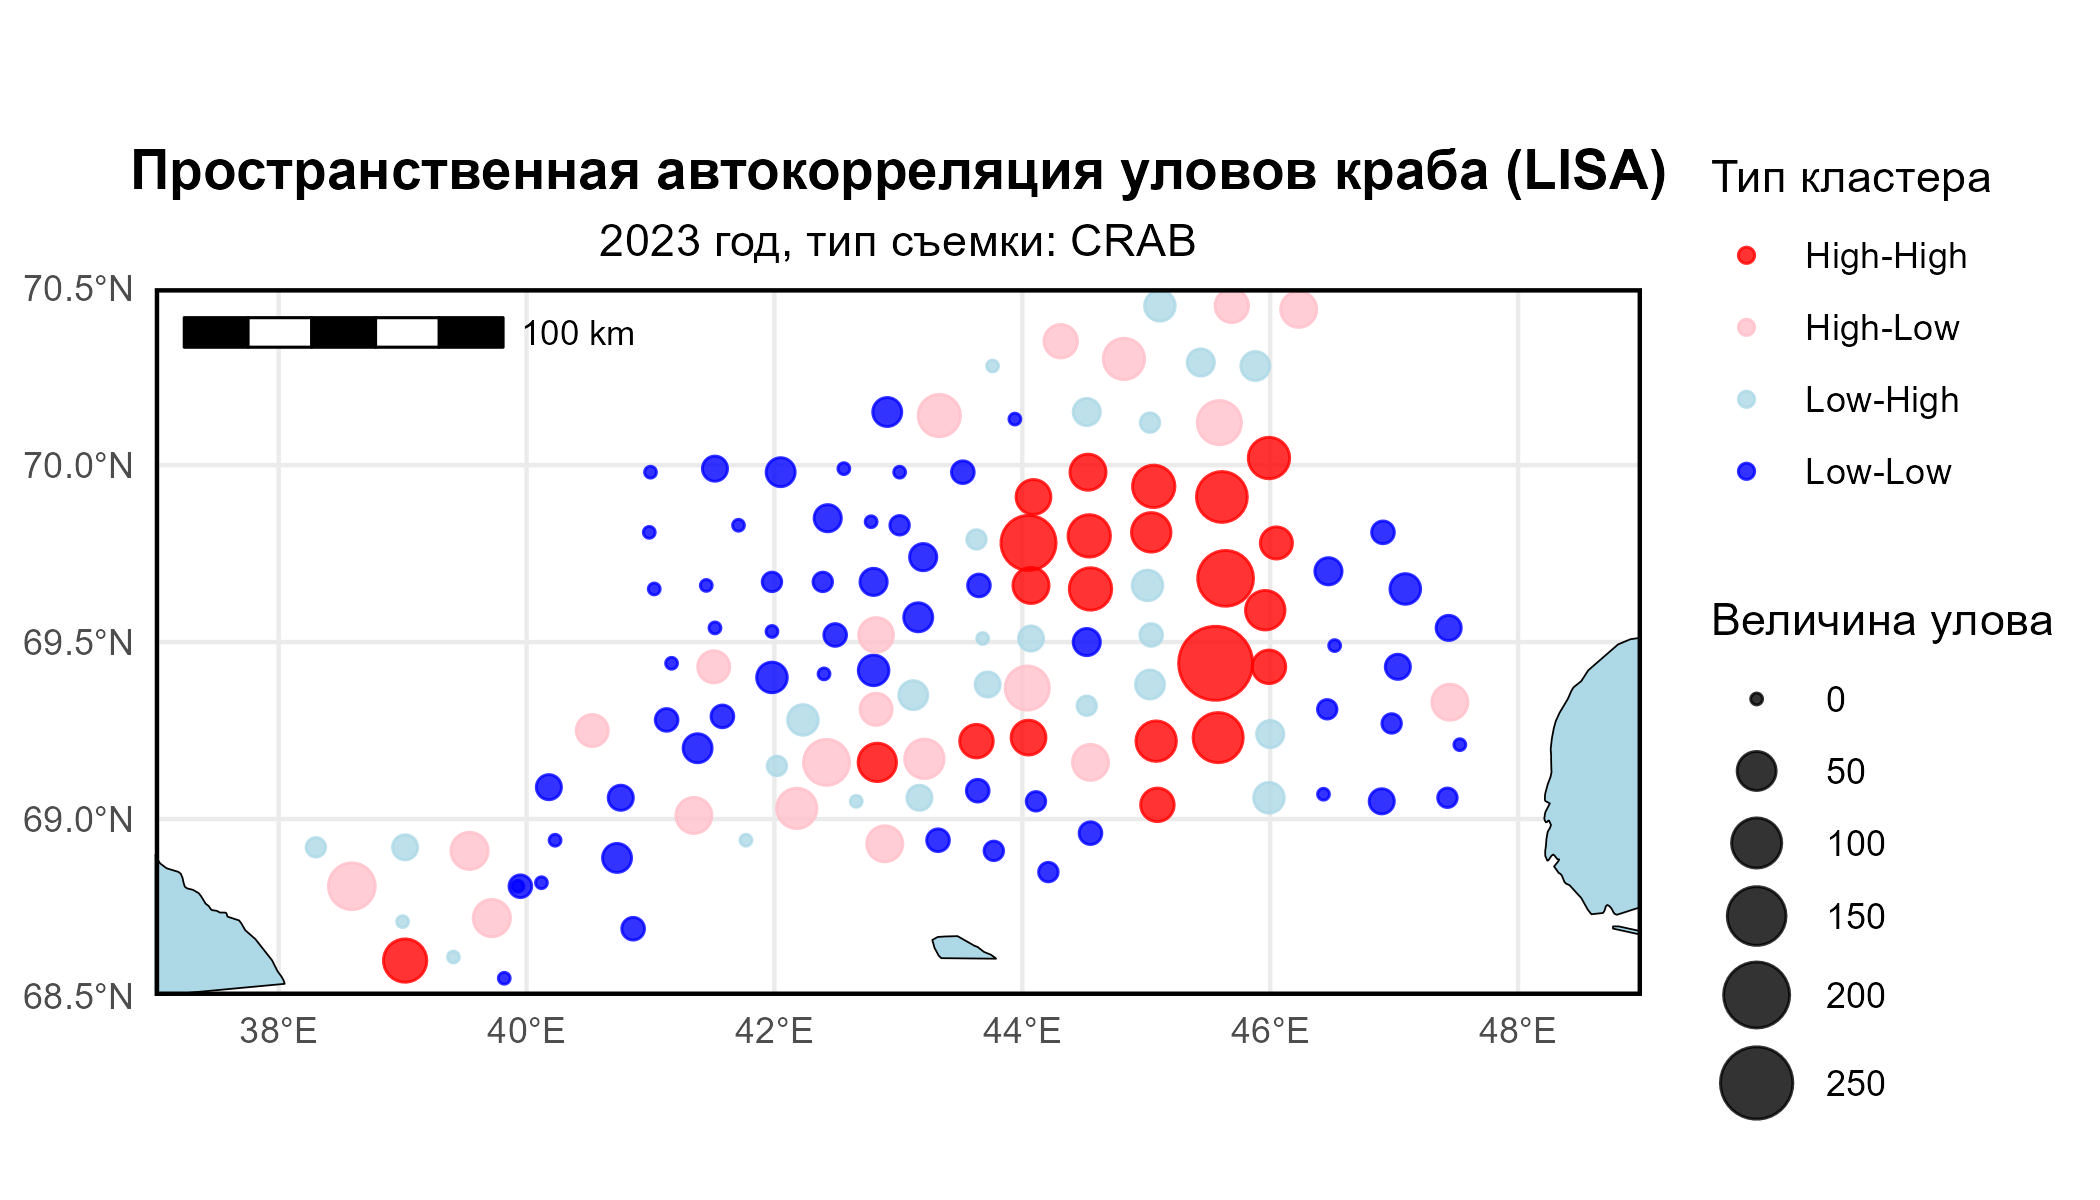
\includegraphics[width=0.8\linewidth,height=\textheight,keepaspectratio]{images/KARTOGRAPH6.jpg}

}

\caption{Рис. 6.: Карта распределения уловов с автокорреляцией LISA}

\end{figure}%

\begin{Shaded}
\begin{Highlighting}[]
\CommentTok{\# Очистка окружения и установка рабочей директории}
\FunctionTok{rm}\NormalTok{(}\AttributeTok{list =} \FunctionTok{ls}\NormalTok{())}
\FunctionTok{setwd}\NormalTok{(}\StringTok{"C:/COURSES/KARTOGRAPH/"}\NormalTok{)}

\CommentTok{\# Загрузка библиотек}
\FunctionTok{library}\NormalTok{(rnaturalearth)}
\FunctionTok{library}\NormalTok{(tidyverse)}
\FunctionTok{library}\NormalTok{(sf)}
\FunctionTok{library}\NormalTok{(spdep)}
\FunctionTok{library}\NormalTok{(ggspatial)}
\FunctionTok{library}\NormalTok{(readxl)}

\CommentTok{\# 1. ЗАГРУЗКА И ПОДГОТОВКА ДАННЫХ}
\NormalTok{DATA }\OtherTok{\textless{}{-}} \FunctionTok{read\_excel}\NormalTok{(}\StringTok{"KARTOGRAPHIC.xlsx"}\NormalTok{, }\AttributeTok{sheet =} \StringTok{"SURVEY"}\NormalTok{) }\SpecialCharTok{\%\textgreater{}\%} 
  \FunctionTok{filter}\NormalTok{(YEAR }\SpecialCharTok{==} \DecValTok{2023}\NormalTok{, SURV }\SpecialCharTok{==} \StringTok{"CRAB"}\NormalTok{)}

\CommentTok{\# Проверка названий колонок}
\FunctionTok{print}\NormalTok{(}\FunctionTok{names}\NormalTok{(DATA))  }\CommentTok{\# Убедитесь, что координаты названы правильно}

\CommentTok{\# Преобразование в пространственные данные (замените X/Y на ваши названия)}
\NormalTok{points\_sf }\OtherTok{\textless{}{-}} \FunctionTok{st\_as\_sf}\NormalTok{(DATA, }\AttributeTok{coords =} \FunctionTok{c}\NormalTok{(}\StringTok{"X"}\NormalTok{, }\StringTok{"Y"}\NormalTok{), }\AttributeTok{crs =} \DecValTok{4326}\NormalTok{)}

\CommentTok{\# 2. ПОЛУЧЕНИЕ КАРТЫ РОССИИ}
\CommentTok{\# Задаем границы области}
\NormalTok{xmin }\OtherTok{\textless{}{-}} \DecValTok{37}
\NormalTok{xmax }\OtherTok{\textless{}{-}} \DecValTok{49}
\NormalTok{ymin }\OtherTok{\textless{}{-}} \FloatTok{68.5}
\NormalTok{ymax }\OtherTok{\textless{}{-}} \FloatTok{70.5}

\CommentTok{\# Создаём ограничивающий прямоугольник}
\NormalTok{bbox }\OtherTok{\textless{}{-}} \FunctionTok{st\_bbox}\NormalTok{(}\FunctionTok{c}\NormalTok{(}\AttributeTok{xmin =}\NormalTok{ xmin, }\AttributeTok{xmax =}\NormalTok{ xmax, }\AttributeTok{ymin =}\NormalTok{ ymin, }\AttributeTok{ymax =}\NormalTok{ ymax), }\AttributeTok{crs =} \DecValTok{4326}\NormalTok{)}
\NormalTok{bbox\_poly }\OtherTok{\textless{}{-}} \FunctionTok{st\_as\_sfc}\NormalTok{(bbox)}

\CommentTok{\# Карта России}
\NormalTok{russia }\OtherTok{\textless{}{-}} \FunctionTok{ne\_countries}\NormalTok{(}\AttributeTok{country =} \StringTok{"Russia"}\NormalTok{, }\AttributeTok{scale =} \DecValTok{10}\NormalTok{) }\SpecialCharTok{\%\textgreater{}\%} 
  \FunctionTok{st\_as\_sf}\NormalTok{() }\SpecialCharTok{\%\textgreater{}\%} 
  \FunctionTok{st\_crop}\NormalTok{(bbox)  }\CommentTok{\# Обрезка без st\_intersection}

\CommentTok{\# 3. ПОДГОТОВКА ТОЧЕК}
\CommentTok{\# Удаление дубликатов по координатам}
\NormalTok{coords }\OtherTok{\textless{}{-}} \FunctionTok{st\_coordinates}\NormalTok{(points\_sf)}
\NormalTok{points\_sf }\OtherTok{\textless{}{-}}\NormalTok{ points\_sf[}\SpecialCharTok{!}\FunctionTok{duplicated}\NormalTok{(coords), , drop }\OtherTok{=} \ConstantTok{FALSE}\NormalTok{]}

\CommentTok{\# Перевод в UTM}
\NormalTok{points\_utm }\OtherTok{\textless{}{-}} \FunctionTok{st\_transform}\NormalTok{(points\_sf, }\AttributeTok{crs =} \DecValTok{32638}\NormalTok{)}

\CommentTok{\# 4. АНАЛИЗ LISA}
\CommentTok{\# Матрица весов}
\NormalTok{knn }\OtherTok{\textless{}{-}} \FunctionTok{knearneigh}\NormalTok{(points\_utm, }\AttributeTok{k =} \DecValTok{4}\NormalTok{)}
\NormalTok{nb }\OtherTok{\textless{}{-}} \FunctionTok{knn2nb}\NormalTok{(knn)}
\NormalTok{listw }\OtherTok{\textless{}{-}} \FunctionTok{nb2listw}\NormalTok{(nb, }\AttributeTok{style =} \StringTok{"W"}\NormalTok{)}

\CommentTok{\# Локальный Моран}
\NormalTok{local\_moran }\OtherTok{\textless{}{-}} \FunctionTok{localmoran}\NormalTok{(points\_utm}\SpecialCharTok{$}\NormalTok{PROM, listw)}

\CommentTok{\# Добавляем кластеры}
\NormalTok{points\_utm }\OtherTok{\textless{}{-}}\NormalTok{ points\_utm }\SpecialCharTok{\%\textgreater{}\%}
  \FunctionTok{mutate}\NormalTok{(}
    \AttributeTok{Local\_I =}\NormalTok{ local\_moran[, }\StringTok{"Ii"}\NormalTok{],}
    \AttributeTok{P\_value =}\NormalTok{ local\_moran[, }\StringTok{"Pr(z != E(Ii))"}\NormalTok{],}
    \AttributeTok{Mean\_PROM =} \FunctionTok{mean}\NormalTok{(PROM, }\AttributeTok{na.rm =} \ConstantTok{TRUE}\NormalTok{),  }\CommentTok{\# Добавляем среднее значение}
    \AttributeTok{Cluster =} \FunctionTok{case\_when}\NormalTok{(}
\NormalTok{      Local\_I }\SpecialCharTok{\textgreater{}} \DecValTok{0} \SpecialCharTok{\&}\NormalTok{ PROM }\SpecialCharTok{\textgreater{}}\NormalTok{ Mean\_PROM }\SpecialCharTok{\textasciitilde{}} \StringTok{"High{-}High"}\NormalTok{,}
\NormalTok{      Local\_I }\SpecialCharTok{\textgreater{}} \DecValTok{0} \SpecialCharTok{\&}\NormalTok{ PROM }\SpecialCharTok{\textless{}=}\NormalTok{ Mean\_PROM }\SpecialCharTok{\textasciitilde{}} \StringTok{"Low{-}Low"}\NormalTok{,  }\CommentTok{\# Включаем PROM == 0}
\NormalTok{      Local\_I }\SpecialCharTok{\textless{}} \DecValTok{0} \SpecialCharTok{\&}\NormalTok{ PROM }\SpecialCharTok{\textgreater{}}\NormalTok{ Mean\_PROM }\SpecialCharTok{\textasciitilde{}} \StringTok{"High{-}Low"}\NormalTok{,}
\NormalTok{      Local\_I }\SpecialCharTok{\textless{}} \DecValTok{0} \SpecialCharTok{\&}\NormalTok{ PROM }\SpecialCharTok{\textless{}=}\NormalTok{ Mean\_PROM }\SpecialCharTok{\textasciitilde{}} \StringTok{"Low{-}High"}\NormalTok{,  }\CommentTok{\# PROM == 0 попадает сюда}
      \ConstantTok{TRUE} \SpecialCharTok{\textasciitilde{}} \StringTok{"Not significant"}
\NormalTok{    )}
\NormalTok{  )}

\CommentTok{\# Обратно в WGS84}
\NormalTok{points\_result }\OtherTok{\textless{}{-}} \FunctionTok{st\_transform}\NormalTok{(points\_utm, }\AttributeTok{crs =} \DecValTok{4326}\NormalTok{)}

\CommentTok{\# 5. ВИЗУАЛИЗАЦИЯ}
\NormalTok{cluster\_colors }\OtherTok{\textless{}{-}} \FunctionTok{c}\NormalTok{(}
  \StringTok{"High{-}High"} \OtherTok{=} \StringTok{"red"}\NormalTok{,}
  \StringTok{"Low{-}Low"} \OtherTok{=} \StringTok{"blue"}\NormalTok{,}
  \StringTok{"High{-}Low"} \OtherTok{=} \StringTok{"pink"}\NormalTok{,}
  \StringTok{"Low{-}High"} \OtherTok{=} \StringTok{"lightblue"}\NormalTok{,}
  \StringTok{"Not significant"} \OtherTok{=} \StringTok{"gray"}
\NormalTok{)}

\FunctionTok{ggplot}\NormalTok{() }\SpecialCharTok{+}
  \CommentTok{\# Карта России}
  \FunctionTok{geom\_sf}\NormalTok{(}\AttributeTok{data =}\NormalTok{ russia, }\AttributeTok{fill =} \StringTok{"lightblue"}\NormalTok{, }\AttributeTok{color =} \StringTok{"black"}\NormalTok{) }\SpecialCharTok{+}
  
  \CommentTok{\# Все точки (включая PROM == 0) — в одном слое}
  \FunctionTok{geom\_sf}\NormalTok{(}
    \AttributeTok{data =}\NormalTok{ points\_result,}
    \FunctionTok{aes}\NormalTok{(}\AttributeTok{color =}\NormalTok{ Cluster, }\AttributeTok{size =}\NormalTok{ PROM),}
    \AttributeTok{alpha =} \FloatTok{0.8}
\NormalTok{  ) }\SpecialCharTok{+}
  
  \CommentTok{\# Настройки координат и масштаба}
  \FunctionTok{coord\_sf}\NormalTok{(}\AttributeTok{xlim =} \FunctionTok{c}\NormalTok{(xmin, xmax), }\AttributeTok{ylim =} \FunctionTok{c}\NormalTok{(ymin, ymax), }\AttributeTok{expand =} \ConstantTok{FALSE}\NormalTok{) }\SpecialCharTok{+}
  \FunctionTok{annotation\_scale}\NormalTok{(}\AttributeTok{location =} \StringTok{"tl"}\NormalTok{, }\AttributeTok{width\_hint =} \FloatTok{0.3}\NormalTok{) }\SpecialCharTok{+}
  
  \CommentTok{\# Цвет и размер}
  \FunctionTok{scale\_color\_manual}\NormalTok{(}\AttributeTok{values =}\NormalTok{ cluster\_colors) }\SpecialCharTok{+}
  \FunctionTok{scale\_size\_continuous}\NormalTok{(}\AttributeTok{range =} \FunctionTok{c}\NormalTok{(}\DecValTok{1}\NormalTok{, }\DecValTok{8}\NormalTok{), }\AttributeTok{name =} \StringTok{"Величина улова"}\NormalTok{) }\SpecialCharTok{+}
  
  \CommentTok{\# Заголовки и тема}
  \FunctionTok{labs}\NormalTok{(}
    \AttributeTok{title =} \StringTok{"Пространственная автокорреляция уловов краба (LISA)"}\NormalTok{,}
    \AttributeTok{subtitle =} \StringTok{"2023 год, тип съемки: CRAB"}\NormalTok{,}
    \AttributeTok{color =} \StringTok{"Тип кластера"}
\NormalTok{  ) }\SpecialCharTok{+}
  
\FunctionTok{theme\_minimal}\NormalTok{() }\SpecialCharTok{+}
  \FunctionTok{theme}\NormalTok{(}
    \AttributeTok{plot.title =} \FunctionTok{element\_text}\NormalTok{(}\AttributeTok{hjust =} \FloatTok{0.5}\NormalTok{, }\AttributeTok{face =} \StringTok{"bold"}\NormalTok{),}
    \AttributeTok{plot.subtitle =} \FunctionTok{element\_text}\NormalTok{(}\AttributeTok{hjust =} \FloatTok{0.5}\NormalTok{),}
    \AttributeTok{legend.position =} \StringTok{"right"}\NormalTok{,}
    \AttributeTok{panel.border =} \FunctionTok{element\_rect}\NormalTok{(}\AttributeTok{colour =} \StringTok{"black"}\NormalTok{, }\AttributeTok{size =} \DecValTok{1}\NormalTok{, }\AttributeTok{fill =} \ConstantTok{NA}\NormalTok{)  }\CommentTok{\# Рамка вокруг карты}
\NormalTok{  )}
\end{Highlighting}
\end{Shaded}

\section{Карта распределения уловов с автокорреляцией LISA по
фасеткам}\label{ux43aux430ux440ux442ux430-ux440ux430ux441ux43fux440ux435ux434ux435ux43bux435ux43dux438ux44f-ux443ux43bux43eux432ux43eux432-ux441-ux430ux432ux442ux43eux43aux43eux440ux440ux435ux43bux44fux446ux438ux435ux439-lisa-ux43fux43e-ux444ux430ux441ux435ux442ux43aux430ux43c}

\begin{figure}[H]

{\centering 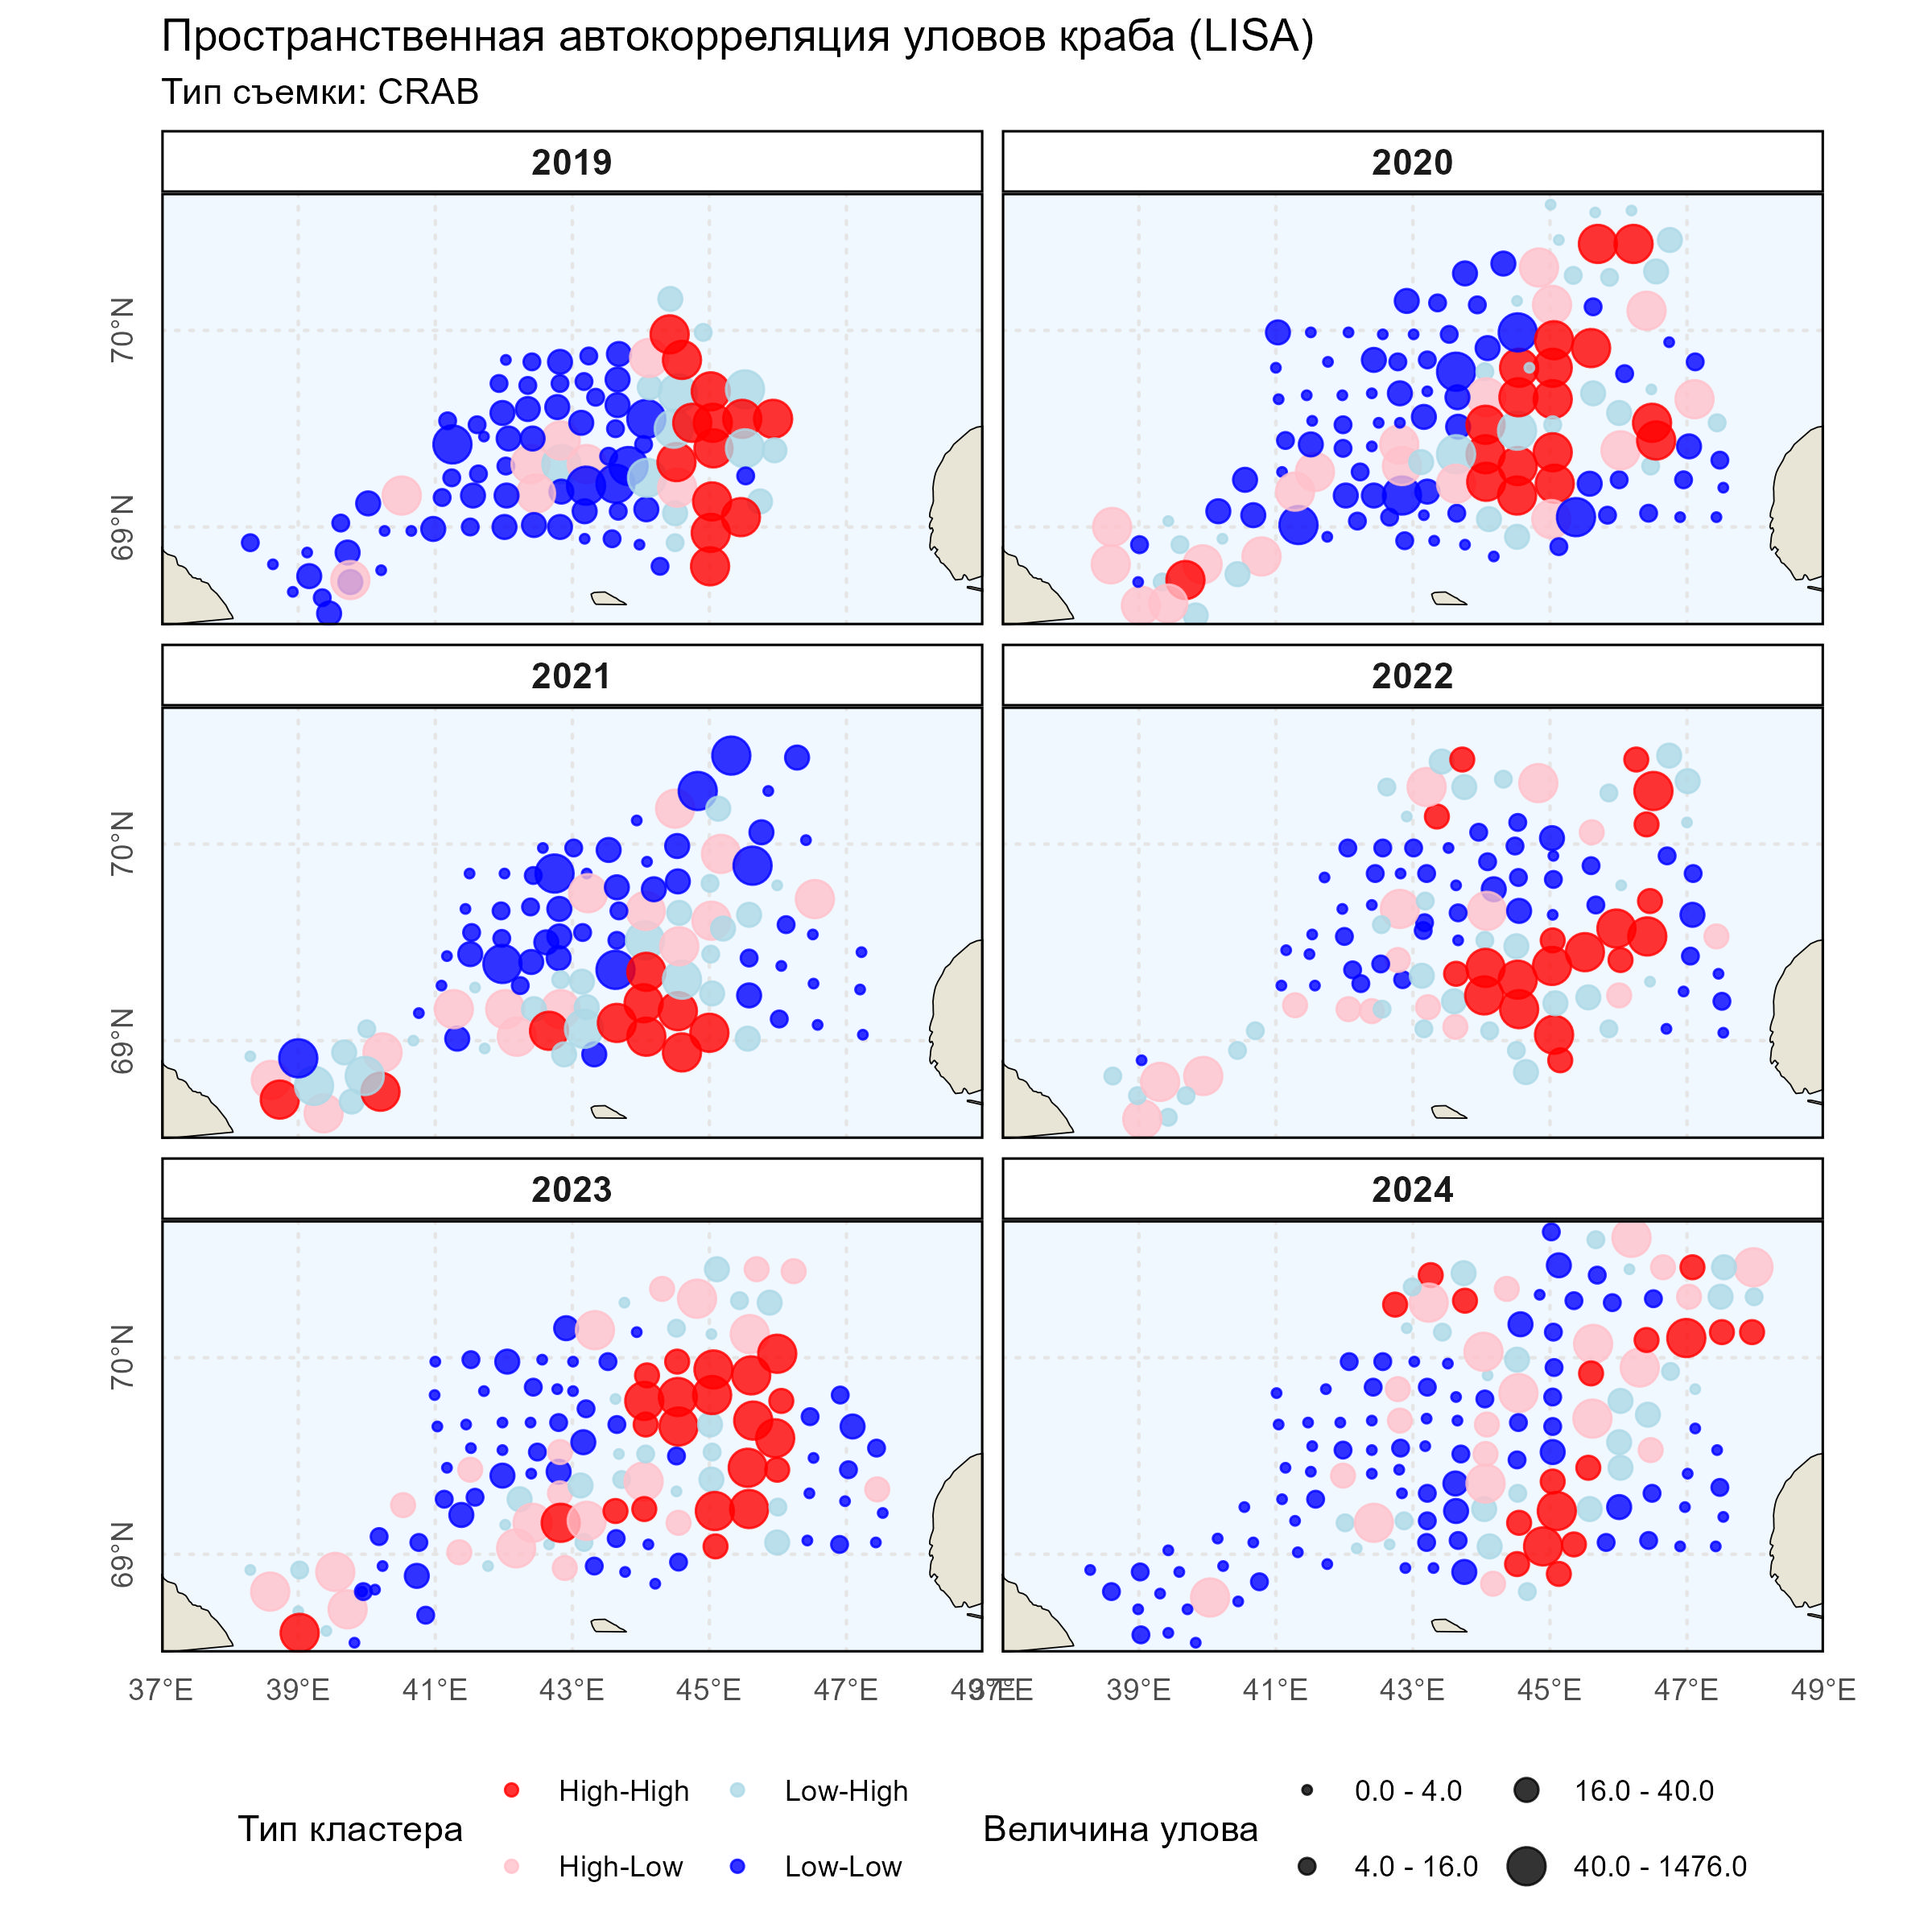
\includegraphics[width=0.8\linewidth,height=\textheight,keepaspectratio]{images/KARTOGRAPH7.jpg}

}

\caption{Рис. 7.: Карта распределения уловов с автокорреляцией LISA по
фасеткам}

\end{figure}%

\begin{Shaded}
\begin{Highlighting}[]
\CommentTok{\# Очистка памяти и установка рабочей папки}
\FunctionTok{rm}\NormalTok{(}\AttributeTok{list =} \FunctionTok{ls}\NormalTok{())}
\FunctionTok{setwd}\NormalTok{(}\StringTok{"C:/COURSES/KARTOGRAPH/"}\NormalTok{)}

\CommentTok{\# Загрузка необходимых пакетов}
\FunctionTok{library}\NormalTok{(rnaturalearth)  }\CommentTok{\# Географические карты}
\FunctionTok{library}\NormalTok{(tidyverse)      }\CommentTok{\# Обработка данных и визуализация}
\FunctionTok{library}\NormalTok{(sf)             }\CommentTok{\# Пространственные данные}
\FunctionTok{library}\NormalTok{(spdep)          }\CommentTok{\# Пространственная статистика}
\FunctionTok{library}\NormalTok{(ggspatial)      }\CommentTok{\# Дополнения для карт в ggplot}
\FunctionTok{library}\NormalTok{(readxl)         }\CommentTok{\# Чтение Excel{-}файлов}

\CommentTok{\# 1. ЗАГРУЗКА И ПРЕОБРАЗОВАНИЕ ДАННЫХ}
\CommentTok{\# {-} Чтение данных из Excel}
\CommentTok{\# {-} Фильтрация только данных по крабу}
\NormalTok{DATA }\OtherTok{\textless{}{-}} \FunctionTok{read\_excel}\NormalTok{(}\StringTok{"KARTOGRAPHIC.xlsx"}\NormalTok{, }\AttributeTok{sheet =} \StringTok{"SURVEY"}\NormalTok{) }\SpecialCharTok{\%\textgreater{}\%} 
  \FunctionTok{filter}\NormalTok{(SURV }\SpecialCharTok{==} \StringTok{"CRAB"}\NormalTok{)}

\CommentTok{\# Преобразование в пространственный объект с координатами}
\NormalTok{points\_sf }\OtherTok{\textless{}{-}} \FunctionTok{st\_as\_sf}\NormalTok{(DATA, }\AttributeTok{coords =} \FunctionTok{c}\NormalTok{(}\StringTok{"X"}\NormalTok{, }\StringTok{"Y"}\NormalTok{), }\AttributeTok{crs =} \DecValTok{4326}\NormalTok{)}

\CommentTok{\# 2. ПОДГОТОВКА КАРТОГРАФИЧЕСКОЙ ОСНОВЫ}
\CommentTok{\# {-} Определение границ области исследования}
\NormalTok{xmin }\OtherTok{\textless{}{-}} \DecValTok{37}\NormalTok{; xmax }\OtherTok{\textless{}{-}} \DecValTok{49}\NormalTok{; ymin }\OtherTok{\textless{}{-}} \FloatTok{68.5}\NormalTok{; ymax }\OtherTok{\textless{}{-}} \FloatTok{70.7}

\CommentTok{\# {-} Создание ограничивающего прямоугольника}
\NormalTok{bbox }\OtherTok{\textless{}{-}} \FunctionTok{st\_bbox}\NormalTok{(}\FunctionTok{c}\NormalTok{(}\AttributeTok{xmin =}\NormalTok{ xmin, }\AttributeTok{xmax =}\NormalTok{ xmax, }\AttributeTok{ymin =}\NormalTok{ ymin, }\AttributeTok{ymax =}\NormalTok{ ymax), }\AttributeTok{crs =} \DecValTok{4326}\NormalTok{)}

\CommentTok{\# {-} Загрузка и обрезка карты России по заданным границам}
\NormalTok{russia }\OtherTok{\textless{}{-}} \FunctionTok{ne\_countries}\NormalTok{(}\AttributeTok{country =} \StringTok{"Russia"}\NormalTok{, }\AttributeTok{scale =} \DecValTok{10}\NormalTok{) }\SpecialCharTok{\%\textgreater{}\%} 
  \FunctionTok{st\_as\_sf}\NormalTok{() }\SpecialCharTok{\%\textgreater{}\%} 
  \FunctionTok{st\_crop}\NormalTok{(bbox)}

\CommentTok{\# 3. ФУНКЦИЯ ДЛЯ ПРОСТРАНСТВЕННОГО АНАЛИЗА ПО ГОДАМ}
\NormalTok{analyze\_year }\OtherTok{\textless{}{-}} \ControlFlowTok{function}\NormalTok{(data\_year) \{}
  \CommentTok{\# Удаление дубликатов координат}
\NormalTok{  coords }\OtherTok{\textless{}{-}} \FunctionTok{st\_coordinates}\NormalTok{(data\_year)}
\NormalTok{  data\_year }\OtherTok{\textless{}{-}}\NormalTok{ data\_year[}\SpecialCharTok{!}\FunctionTok{duplicated}\NormalTok{(coords), , drop }\OtherTok{=} \ConstantTok{FALSE}\NormalTok{]}
  
  \CommentTok{\# Перепроецирование в UTM для точных расчетов}
\NormalTok{  points\_utm }\OtherTok{\textless{}{-}} \FunctionTok{st\_transform}\NormalTok{(data\_year, }\AttributeTok{crs =} \DecValTok{32638}\NormalTok{)}
  
  \CommentTok{\# Построение матрицы пространственных весов (4 ближайших соседа)}
\NormalTok{  knn }\OtherTok{\textless{}{-}} \FunctionTok{knearneigh}\NormalTok{(points\_utm, }\AttributeTok{k =} \DecValTok{4}\NormalTok{)}
\NormalTok{  nb }\OtherTok{\textless{}{-}} \FunctionTok{knn2nb}\NormalTok{(knn)}
\NormalTok{  listw }\OtherTok{\textless{}{-}} \FunctionTok{nb2listw}\NormalTok{(nb, }\AttributeTok{style =} \StringTok{"W"}\NormalTok{)  }\CommentTok{\# Стандартизованная матрица}
  
  \CommentTok{\# Расчет локальной пространственной автокорреляции (LISA)}
\NormalTok{  local\_moran }\OtherTok{\textless{}{-}} \FunctionTok{localmoran}\NormalTok{(points\_utm}\SpecialCharTok{$}\NormalTok{PROM, listw)}
  
  \CommentTok{\# Классификация кластеров на основе результатов}
\NormalTok{  points\_utm }\OtherTok{\textless{}{-}}\NormalTok{ points\_utm }\SpecialCharTok{\%\textgreater{}\%}
    \FunctionTok{mutate}\NormalTok{(}
      \AttributeTok{Local\_I =}\NormalTok{ local\_moran[, }\StringTok{"Ii"}\NormalTok{],}
      \AttributeTok{P\_value =}\NormalTok{ local\_moran[, }\StringTok{"Pr(z != E(Ii))"}\NormalTok{],}
      \AttributeTok{Mean\_PROM =} \FunctionTok{mean}\NormalTok{(PROM, }\AttributeTok{na.rm =} \ConstantTok{TRUE}\NormalTok{),}
      \AttributeTok{Cluster =} \FunctionTok{case\_when}\NormalTok{(}
\NormalTok{        Local\_I }\SpecialCharTok{\textgreater{}} \DecValTok{0} \SpecialCharTok{\&}\NormalTok{ PROM }\SpecialCharTok{\textgreater{}}\NormalTok{ Mean\_PROM }\SpecialCharTok{\textasciitilde{}} \StringTok{"High{-}High"}\NormalTok{,     }\CommentTok{\# Горячая точка}
\NormalTok{        Local\_I }\SpecialCharTok{\textgreater{}} \DecValTok{0} \SpecialCharTok{\&}\NormalTok{ PROM }\SpecialCharTok{\textless{}=}\NormalTok{ Mean\_PROM }\SpecialCharTok{\textasciitilde{}} \StringTok{"Low{-}Low"}\NormalTok{,      }\CommentTok{\# Холодная точка}
\NormalTok{        Local\_I }\SpecialCharTok{\textless{}} \DecValTok{0} \SpecialCharTok{\&}\NormalTok{ PROM }\SpecialCharTok{\textgreater{}}\NormalTok{ Mean\_PROM }\SpecialCharTok{\textasciitilde{}} \StringTok{"High{-}Low"}\NormalTok{,      }\CommentTok{\# Выброс (высокий среди низких)}
\NormalTok{        Local\_I }\SpecialCharTok{\textless{}} \DecValTok{0} \SpecialCharTok{\&}\NormalTok{ PROM }\SpecialCharTok{\textless{}=}\NormalTok{ Mean\_PROM }\SpecialCharTok{\textasciitilde{}} \StringTok{"Low{-}High"}\NormalTok{,     }\CommentTok{\# Выброс (низкий среди высоких)}
        \ConstantTok{TRUE} \SpecialCharTok{\textasciitilde{}} \StringTok{"Not significant"}                          \CommentTok{\# Незначимые}
\NormalTok{      )}
\NormalTok{    )}
  
  \CommentTok{\# Возврат в географические координаты}
  \FunctionTok{st\_transform}\NormalTok{(points\_utm, }\AttributeTok{crs =} \DecValTok{4326}\NormalTok{)}
\NormalTok{\}}

\CommentTok{\# 4. ОБРАБОТКА ДАННЫХ ПО ГОДАМ}
\CommentTok{\# {-} Разделение данных по годам}
\CommentTok{\# {-} Применение анализа для каждого года}
\CommentTok{\# {-} Объединение результатов}
\NormalTok{results\_list }\OtherTok{\textless{}{-}}\NormalTok{ DATA }\SpecialCharTok{\%\textgreater{}\%}
  \FunctionTok{group\_split}\NormalTok{(YEAR) }\SpecialCharTok{\%\textgreater{}\%} 
  \FunctionTok{lapply}\NormalTok{(}\ControlFlowTok{function}\NormalTok{(group) \{}
    \FunctionTok{analyze\_year}\NormalTok{(}\FunctionTok{st\_as\_sf}\NormalTok{(group, }\AttributeTok{coords =} \FunctionTok{c}\NormalTok{(}\StringTok{"X"}\NormalTok{, }\StringTok{"Y"}\NormalTok{), }\AttributeTok{crs =} \DecValTok{4326}\NormalTok{))}
\NormalTok{  \}) }\SpecialCharTok{\%\textgreater{}\%}
  \FunctionTok{bind\_rows}\NormalTok{()}

\CommentTok{\# 5. КАТЕГОРИЗАЦИЯ УЛОВОВ}
\CommentTok{\# {-} Расчет квантилей для всего набора данных}
\NormalTok{PROM\_breaks }\OtherTok{\textless{}{-}} \FunctionTok{quantile}\NormalTok{(results\_list}\SpecialCharTok{$}\NormalTok{PROM, }
                         \AttributeTok{probs =} \FunctionTok{c}\NormalTok{(}\DecValTok{0}\NormalTok{, }\FloatTok{0.25}\NormalTok{, }\FloatTok{0.5}\NormalTok{, }\FloatTok{0.75}\NormalTok{, }\DecValTok{1}\NormalTok{), }
                         \AttributeTok{na.rm =} \ConstantTok{TRUE}\NormalTok{) }\SpecialCharTok{\%\textgreater{}\%} 
  \FunctionTok{round}\NormalTok{(}\DecValTok{1}\NormalTok{)  }\CommentTok{\# Округление значений}

\CommentTok{\# {-} Создание меток с реальными диапазонами}
\NormalTok{PROM\_labels }\OtherTok{\textless{}{-}} \FunctionTok{sprintf}\NormalTok{(}\StringTok{"\%.1f {-} \%.1f"}\NormalTok{, PROM\_breaks[}\DecValTok{1}\SpecialCharTok{:}\DecValTok{4}\NormalTok{], PROM\_breaks[}\DecValTok{2}\SpecialCharTok{:}\DecValTok{5}\NormalTok{])}

\CommentTok{\# {-} Добавление категорий уловов в данные}
\NormalTok{results\_list }\OtherTok{\textless{}{-}}\NormalTok{ results\_list }\SpecialCharTok{\%\textgreater{}\%}
  \FunctionTok{mutate}\NormalTok{(}
    \AttributeTok{PROM\_category =} \FunctionTok{cut}\NormalTok{(}
\NormalTok{      PROM, }
      \AttributeTok{breaks =}\NormalTok{ PROM\_breaks, }
      \AttributeTok{labels =}\NormalTok{ PROM\_labels,}
      \AttributeTok{include.lowest =} \ConstantTok{TRUE}
\NormalTok{    )}
\NormalTok{  )}

\CommentTok{\# 6. ВИЗУАЛИЗАЦИЯ РЕЗУЛЬТАТОВ}
\CommentTok{\# Цветовая схема для типов кластеров}
\NormalTok{cluster\_colors }\OtherTok{\textless{}{-}} \FunctionTok{c}\NormalTok{(}
  \StringTok{"High{-}High"} \OtherTok{=} \StringTok{"red"}\NormalTok{,       }\CommentTok{\# Горячие точки}
  \StringTok{"Low{-}Low"} \OtherTok{=} \StringTok{"blue"}\NormalTok{,        }\CommentTok{\# Холодные точки}
  \StringTok{"High{-}Low"} \OtherTok{=} \StringTok{"pink"}\NormalTok{,       }\CommentTok{\# Выбросы высокие}
  \StringTok{"Low{-}High"} \OtherTok{=} \StringTok{"lightblue"}\NormalTok{,  }\CommentTok{\# Выбросы низкие}
  \StringTok{"Not significant"} \OtherTok{=} \StringTok{"gray"} \CommentTok{\# Незначимые}
\NormalTok{)}

\CommentTok{\# Построение карты}
\FunctionTok{ggplot}\NormalTok{(}\AttributeTok{data =}\NormalTok{ results\_list) }\SpecialCharTok{+}
  \CommentTok{\# Базовая карта России}
  \FunctionTok{geom\_sf}\NormalTok{(}\AttributeTok{data =}\NormalTok{ russia, }\AttributeTok{fill =} \StringTok{"\#E8E5D6"}\NormalTok{, }\AttributeTok{color =} \StringTok{"black"}\NormalTok{, }\AttributeTok{inherit.aes =} \ConstantTok{FALSE}\NormalTok{) }\SpecialCharTok{+}
  
  \CommentTok{\# Точки наблюдений с цветом по кластерам и размером по уловам}
  \FunctionTok{geom\_sf}\NormalTok{(}\FunctionTok{aes}\NormalTok{(}\AttributeTok{color =}\NormalTok{ Cluster, }\AttributeTok{size =}\NormalTok{ PROM\_category), }\AttributeTok{alpha =} \FloatTok{0.8}\NormalTok{) }\SpecialCharTok{+}
  
  \CommentTok{\# Разделение на панели по годам}
  \FunctionTok{facet\_wrap}\NormalTok{(}\SpecialCharTok{\textasciitilde{}}\NormalTok{ YEAR, }\AttributeTok{ncol =} \DecValTok{2}\NormalTok{) }\SpecialCharTok{+}
  
  \CommentTok{\# Установка границ карты}
  \FunctionTok{coord\_sf}\NormalTok{(}\AttributeTok{xlim =} \FunctionTok{c}\NormalTok{(xmin, xmax), }\AttributeTok{ylim =} \FunctionTok{c}\NormalTok{(ymin, ymax), }\AttributeTok{expand =} \ConstantTok{FALSE}\NormalTok{) }\SpecialCharTok{+}
  
  \CommentTok{\# Настройка легенды для кластеров}
  \FunctionTok{scale\_color\_manual}\NormalTok{(}
    \AttributeTok{values =}\NormalTok{ cluster\_colors,}
    \AttributeTok{name =} \StringTok{"Тип кластера"}\NormalTok{,}
    \AttributeTok{guide =} \FunctionTok{guide\_legend}\NormalTok{(}\AttributeTok{nrow =} \DecValTok{2}\NormalTok{)}
\NormalTok{  ) }\SpecialCharTok{+}
  
  \CommentTok{\# Настройка легенды для уловов (реальные диапазоны)}
  \FunctionTok{scale\_size\_manual}\NormalTok{(}
    \AttributeTok{name =} \StringTok{"Величина улова"}\NormalTok{,}
    \AttributeTok{values =} \FunctionTok{c}\NormalTok{(}\DecValTok{1}\NormalTok{, }\DecValTok{2}\NormalTok{, }\DecValTok{3}\NormalTok{, }\DecValTok{5}\NormalTok{),  }\CommentTok{\# Размеры точек для 4{-}х категорий}
    \AttributeTok{breaks =} \FunctionTok{levels}\NormalTok{(results\_list}\SpecialCharTok{$}\NormalTok{PROM\_category),}
    \AttributeTok{guide =} \FunctionTok{guide\_legend}\NormalTok{(}\AttributeTok{nrow =} \DecValTok{2}\NormalTok{)}
\NormalTok{  ) }\SpecialCharTok{+}
  
  \CommentTok{\# Заголовки и подписи}
  \FunctionTok{labs}\NormalTok{(}
    \AttributeTok{title =} \StringTok{"Пространственная автокорреляция уловов краба (LISA)"}\NormalTok{,}
    \AttributeTok{subtitle =} \StringTok{"Тип съемки: CRAB"}
\NormalTok{  ) }\SpecialCharTok{+}
  
  \CommentTok{\# Оформление графика}
  \FunctionTok{theme\_minimal}\NormalTok{() }\SpecialCharTok{+}
  \FunctionTok{theme}\NormalTok{(}
    \AttributeTok{axis.text.x =} \FunctionTok{element\_text}\NormalTok{(}\AttributeTok{size =} \DecValTok{9}\NormalTok{, }\AttributeTok{margin =} \FunctionTok{margin}\NormalTok{(}\AttributeTok{t =} \DecValTok{5}\NormalTok{)),}
    \AttributeTok{axis.text.y =} \FunctionTok{element\_text}\NormalTok{(}\AttributeTok{size =} \DecValTok{9}\NormalTok{, }\AttributeTok{angle =} \DecValTok{90}\NormalTok{, }\AttributeTok{hjust =} \FloatTok{0.5}\NormalTok{, }\AttributeTok{margin =} \FunctionTok{margin}\NormalTok{(}\AttributeTok{r =} \DecValTok{5}\NormalTok{)),}
    \AttributeTok{panel.background =} \FunctionTok{element\_rect}\NormalTok{(}\AttributeTok{fill =} \StringTok{"\#F0F8FF"}\NormalTok{, }\AttributeTok{color =} \ConstantTok{NA}\NormalTok{),  }\CommentTok{\# Фон океана}
    \AttributeTok{panel.grid.major =} \FunctionTok{element\_line}\NormalTok{(}\AttributeTok{color =} \StringTok{"grey90"}\NormalTok{, }\AttributeTok{linetype =} \StringTok{"dotted"}\NormalTok{),}
    \AttributeTok{legend.position =} \StringTok{"bottom"}\NormalTok{,           }\CommentTok{\# Легенда внизу}
    \AttributeTok{legend.box =} \StringTok{"horizontal"}\NormalTok{,            }\CommentTok{\# Горизонтальное расположение}
    \AttributeTok{panel.border =} \FunctionTok{element\_rect}\NormalTok{(}\AttributeTok{fill =} \ConstantTok{NA}\NormalTok{, }\AttributeTok{color =} \StringTok{"black"}\NormalTok{, }\AttributeTok{size =} \FloatTok{0.7}\NormalTok{),}
    \AttributeTok{strip.background =} \FunctionTok{element\_rect}\NormalTok{(}\AttributeTok{fill =} \StringTok{"white"}\NormalTok{, }\AttributeTok{color =} \StringTok{"black"}\NormalTok{, }\AttributeTok{size =} \FloatTok{0.7}\NormalTok{),  }\CommentTok{\# Заголовки панелей}
    \AttributeTok{strip.text =} \FunctionTok{element\_text}\NormalTok{(}\AttributeTok{size =} \DecValTok{11}\NormalTok{, }\AttributeTok{face =} \StringTok{"bold"}\NormalTok{)}
\NormalTok{  ) }\SpecialCharTok{+}
  
  \CommentTok{\# Разметка осей (долгота с шагом 2°, широта с шагом 1°)}
  \FunctionTok{scale\_x\_continuous}\NormalTok{(}
    \AttributeTok{breaks =} \FunctionTok{seq}\NormalTok{(}\FunctionTok{floor}\NormalTok{(xmin), }\FunctionTok{ceiling}\NormalTok{(xmax), }\AttributeTok{by =} \DecValTok{2}\NormalTok{),}
    \AttributeTok{labels =} \ControlFlowTok{function}\NormalTok{(x) }\FunctionTok{paste0}\NormalTok{(x, }\StringTok{"°E"}\NormalTok{)}
\NormalTok{  ) }\SpecialCharTok{+}
  \FunctionTok{scale\_y\_continuous}\NormalTok{(}
    \AttributeTok{breaks =} \FunctionTok{seq}\NormalTok{(}\FunctionTok{floor}\NormalTok{(ymin), }\FunctionTok{ceiling}\NormalTok{(ymax), }\AttributeTok{by =} \DecValTok{1}\NormalTok{),  }
    \AttributeTok{labels =} \ControlFlowTok{function}\NormalTok{(y) }\FunctionTok{paste0}\NormalTok{(y, }\StringTok{"°N"}\NormalTok{)}
\NormalTok{  )}
\end{Highlighting}
\end{Shaded}

\section{Промысловые карты с квартильным распределением
уловов}\label{ux43fux440ux43eux43cux44bux441ux43bux43eux432ux44bux435-ux43aux430ux440ux442ux44b-ux441-ux43aux432ux430ux440ux442ux438ux43bux44cux43dux44bux43c-ux440ux430ux441ux43fux440ux435ux434ux435ux43bux435ux43dux438ux435ux43c-ux443ux43bux43eux432ux43eux432}

\begin{figure}[H]

{\centering 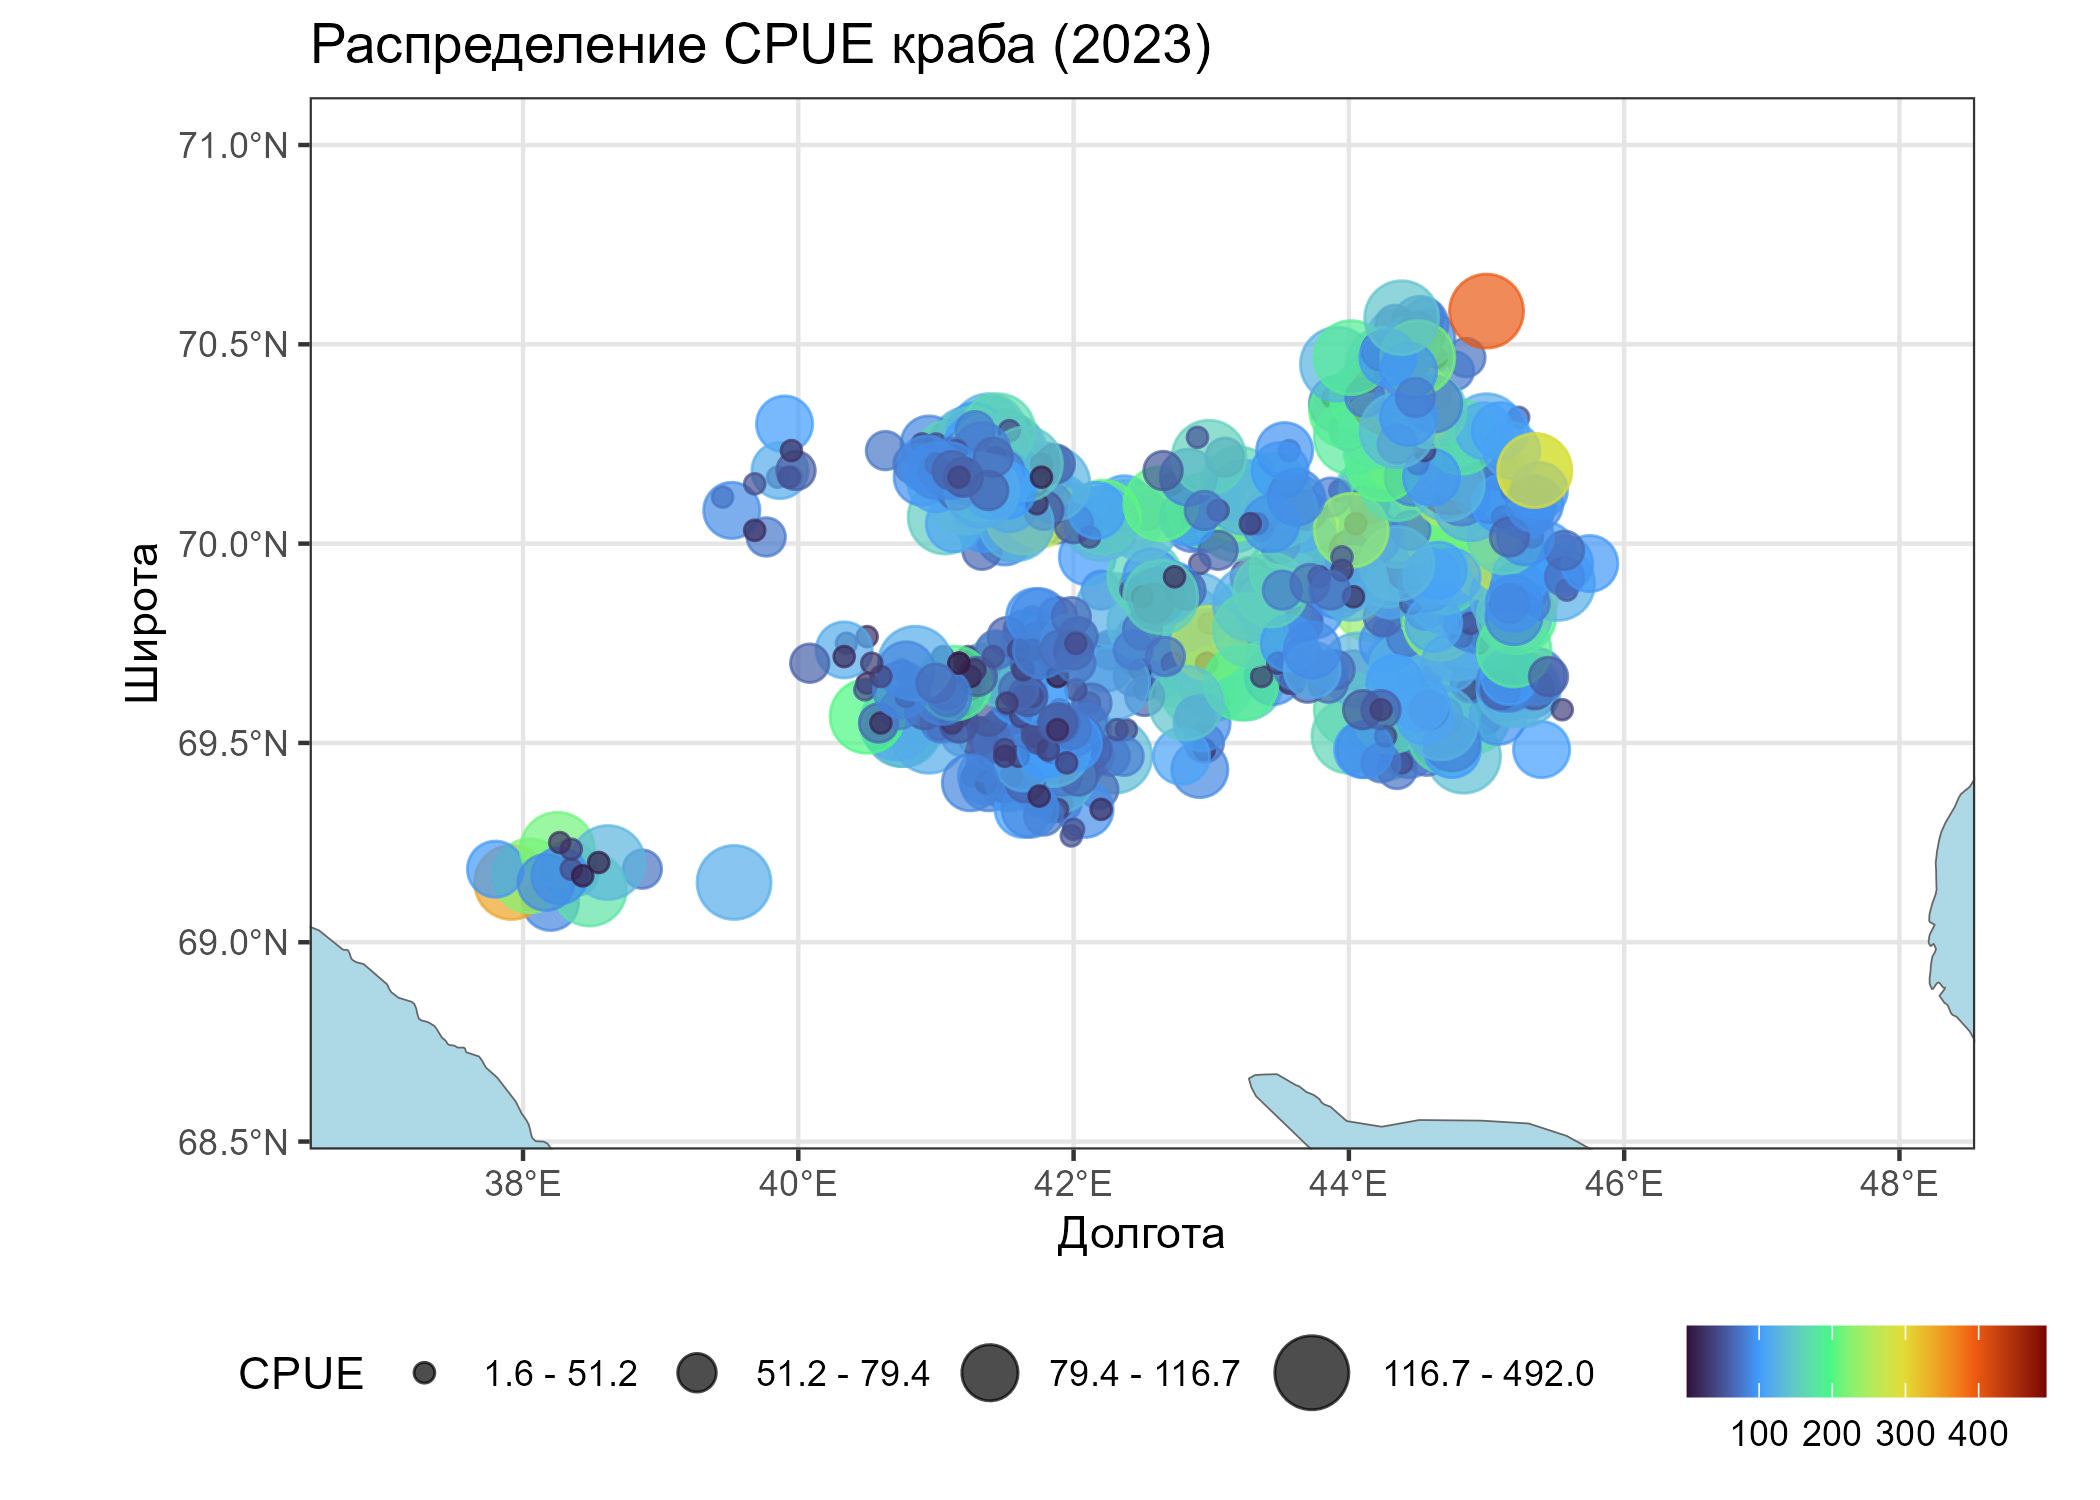
\includegraphics[width=0.8\linewidth,height=\textheight,keepaspectratio]{images/KARTOGRAPH8.jpg}

}

\caption{Рис. 8.: Промысловые карты с квартильным распределением уловов}

\end{figure}%

\begin{Shaded}
\begin{Highlighting}[]
\CommentTok{\# Очистка окружения и установка рабочей директории}
\FunctionTok{rm}\NormalTok{(}\AttributeTok{list =} \FunctionTok{ls}\NormalTok{())}
\FunctionTok{setwd}\NormalTok{(}\StringTok{"C:/COURSES/KARTOGRAPH/"}\NormalTok{)}

\CommentTok{\# Загрузка необходимых библиотек}
\FunctionTok{library}\NormalTok{(rnaturalearth)}
\FunctionTok{library}\NormalTok{(tidyverse)}
\FunctionTok{library}\NormalTok{(sf)}

\DocumentationTok{\#\#\#\#\#\#\# ЗАГРУЗКА ДАННЫХ И ПОДГОТОВКА ПРОСТРАНСТВЕННЫХ ОБЪЕКТОВ \#\#\#\#\#\#\#\#\#\#\#\#\#\#\#\#}

\CommentTok{\# Чтение и фильтрация данных}
\NormalTok{DATA }\OtherTok{\textless{}{-}}\NormalTok{ readxl}\SpecialCharTok{::}\FunctionTok{read\_excel}\NormalTok{(}\StringTok{"KARTOGRAPHIC.xlsx"}\NormalTok{, }\AttributeTok{sheet =} \StringTok{"FISHERY"}\NormalTok{) }\SpecialCharTok{\%\textgreater{}\%} 
  \FunctionTok{filter}\NormalTok{(YEAR }\SpecialCharTok{==} \DecValTok{2023}\NormalTok{)}

\CommentTok{\# Получение границ России}
\NormalTok{russia }\OtherTok{\textless{}{-}} \FunctionTok{ne\_countries}\NormalTok{(}\AttributeTok{scale =} \DecValTok{10}\NormalTok{, }\AttributeTok{country =} \StringTok{"Russia"}\NormalTok{) }\SpecialCharTok{\%\textgreater{}\%} 
  \FunctionTok{st\_as\_sf}\NormalTok{()}

\CommentTok{\# Установка границ отображаемой области}
\NormalTok{xmin}\OtherTok{=}\DecValTok{37}\NormalTok{; xmax}\OtherTok{=}\DecValTok{48}\NormalTok{; ymin}\OtherTok{=}\FloatTok{68.6}\NormalTok{; ymax}\OtherTok{=}\DecValTok{71}

\DocumentationTok{\#\#\#\#\#\#\# ПОДГОТОВКА ДАННЫХ ДЛЯ ВИЗУАЛИЗАЦИИ \#\#\#\#\#\#\#\#\#\#\#\#\#\#\#\#}
\CommentTok{\# Вычисляем квартили отдельно}
\NormalTok{quantiles }\OtherTok{\textless{}{-}} \FunctionTok{quantile}\NormalTok{(DATA}\SpecialCharTok{$}\NormalTok{CPUE[DATA}\SpecialCharTok{$}\NormalTok{CPUE }\SpecialCharTok{\textgreater{}} \DecValTok{0}\NormalTok{], }\AttributeTok{probs =} \FunctionTok{seq}\NormalTok{(}\DecValTok{0}\NormalTok{, }\DecValTok{1}\NormalTok{, }\FloatTok{0.25}\NormalTok{))}

\CommentTok{\# Создаем 4 категории с реальными диапазонами значений}
\NormalTok{nonzero\_data }\OtherTok{\textless{}{-}}\NormalTok{ DATA }\SpecialCharTok{\%\textgreater{}\%} 
  \FunctionTok{filter}\NormalTok{(CPUE }\SpecialCharTok{\textgreater{}} \DecValTok{0}\NormalTok{) }\SpecialCharTok{\%\textgreater{}\%}
  \FunctionTok{mutate}\NormalTok{(}
    \AttributeTok{CPUE\_cat =} \FunctionTok{cut}\NormalTok{(}
\NormalTok{      CPUE,}
      \AttributeTok{breaks =}\NormalTok{ quantiles,}
      \AttributeTok{include.lowest =} \ConstantTok{TRUE}\NormalTok{,}
      \AttributeTok{labels =} \FunctionTok{c}\NormalTok{(}
        \FunctionTok{sprintf}\NormalTok{(}\StringTok{"\%.1f {-} \%.1f"}\NormalTok{, quantiles[}\DecValTok{1}\NormalTok{], quantiles[}\DecValTok{2}\NormalTok{]),}
        \FunctionTok{sprintf}\NormalTok{(}\StringTok{"\%.1f {-} \%.1f"}\NormalTok{, quantiles[}\DecValTok{2}\NormalTok{], quantiles[}\DecValTok{3}\NormalTok{]),}
        \FunctionTok{sprintf}\NormalTok{(}\StringTok{"\%.1f {-} \%.1f"}\NormalTok{, quantiles[}\DecValTok{3}\NormalTok{], quantiles[}\DecValTok{4}\NormalTok{]),}
        \FunctionTok{sprintf}\NormalTok{(}\StringTok{"\%.1f {-} \%.1f"}\NormalTok{, quantiles[}\DecValTok{4}\NormalTok{], quantiles[}\DecValTok{5}\NormalTok{])}
\NormalTok{      )}
\NormalTok{    )}
\NormalTok{  )}

\CommentTok{\# Построение карты}
\FunctionTok{ggplot}\NormalTok{() }\SpecialCharTok{+}
  \CommentTok{\# Базовая карта России}
  \FunctionTok{geom\_sf}\NormalTok{(}\AttributeTok{data =}\NormalTok{ russia, }\AttributeTok{fill =} \StringTok{"lightblue"}\NormalTok{, }\AttributeTok{color =} \StringTok{"gray40"}\NormalTok{) }\SpecialCharTok{+} 
  \CommentTok{\# Ограничение области отображения}
  \FunctionTok{coord\_sf}\NormalTok{(}\AttributeTok{xlim =} \FunctionTok{c}\NormalTok{(xmin, xmax), }\AttributeTok{ylim =} \FunctionTok{c}\NormalTok{(ymin, ymax)) }\SpecialCharTok{+}
  \CommentTok{\# Точки наблюдений с категориальным размером}
  \FunctionTok{geom\_point}\NormalTok{(}
    \AttributeTok{data =}\NormalTok{ nonzero\_data,}
    \FunctionTok{aes}\NormalTok{(}\AttributeTok{x =}\NormalTok{ X, }\AttributeTok{y =}\NormalTok{ Y, }\AttributeTok{size =}\NormalTok{ CPUE\_cat, }\AttributeTok{color =}\NormalTok{ CPUE),}
    \AttributeTok{alpha =} \FloatTok{0.7}
\NormalTok{  ) }\SpecialCharTok{+}
  \CommentTok{\# Точки для нулевых уловов (крестики)}
  \FunctionTok{geom\_point}\NormalTok{(}
    \AttributeTok{data =} \FunctionTok{filter}\NormalTok{(DATA, CPUE }\SpecialCharTok{==} \DecValTok{0}\NormalTok{),}
    \FunctionTok{aes}\NormalTok{(}\AttributeTok{x =}\NormalTok{ X, }\AttributeTok{y =}\NormalTok{ Y),}
    \AttributeTok{shape =} \DecValTok{4}\NormalTok{, }\AttributeTok{size =} \FloatTok{1.2}\NormalTok{, }\AttributeTok{stroke =} \DecValTok{1}\NormalTok{, }\AttributeTok{color =} \StringTok{"black"}
\NormalTok{  ) }\SpecialCharTok{+}
  \CommentTok{\# Цветовая шкала (непрерывная)}
  \FunctionTok{scale\_color\_viridis\_c}\NormalTok{(}\AttributeTok{option =} \StringTok{"H"}\NormalTok{, }\AttributeTok{name =} \ConstantTok{NULL}\NormalTok{) }\SpecialCharTok{+}
  \CommentTok{\# Ручная настройка размеров для категорий}
  \FunctionTok{scale\_size\_manual}\NormalTok{(}
    \AttributeTok{name =} \StringTok{"CPUE"}\NormalTok{,}
    \AttributeTok{values =} \FunctionTok{c}\NormalTok{(}\DecValTok{2}\NormalTok{, }\DecValTok{4}\NormalTok{, }\DecValTok{6}\NormalTok{, }\DecValTok{8}\NormalTok{),  }\CommentTok{\# Размеры точек для категорий}
    \AttributeTok{drop =} \ConstantTok{FALSE}
\NormalTok{  ) }\SpecialCharTok{+}
  \CommentTok{\# Настройки темы}
  \FunctionTok{theme\_bw}\NormalTok{() }\SpecialCharTok{+}
  \FunctionTok{labs}\NormalTok{(}
    \AttributeTok{title =} \StringTok{"Распределение CPUE краба (2023)"}\NormalTok{,}
    \AttributeTok{subtitle =} \ConstantTok{NULL}\NormalTok{,}
    \AttributeTok{x =} \StringTok{"Долгота"}\NormalTok{, }
    \AttributeTok{y =} \StringTok{"Широта"}
\NormalTok{  ) }\SpecialCharTok{+}
  \FunctionTok{theme}\NormalTok{(}
    \AttributeTok{panel.grid =} \FunctionTok{element\_line}\NormalTok{(}\AttributeTok{color =} \StringTok{"gray90"}\NormalTok{),}
    \AttributeTok{legend.position =} \StringTok{"bottom"}
\NormalTok{  )}
\end{Highlighting}
\end{Shaded}

\section{Промысловые карты с агрегацией в центрах полигонов
(промквадратов)}\label{ux43fux440ux43eux43cux44bux441ux43bux43eux432ux44bux435-ux43aux430ux440ux442ux44b-ux441-ux430ux433ux440ux435ux433ux430ux446ux438ux435ux439-ux432-ux446ux435ux43dux442ux440ux430ux445-ux43fux43eux43bux438ux433ux43eux43dux43eux432-ux43fux440ux43eux43cux43aux432ux430ux434ux440ux430ux442ux43eux432}

\begin{figure}[H]

{\centering 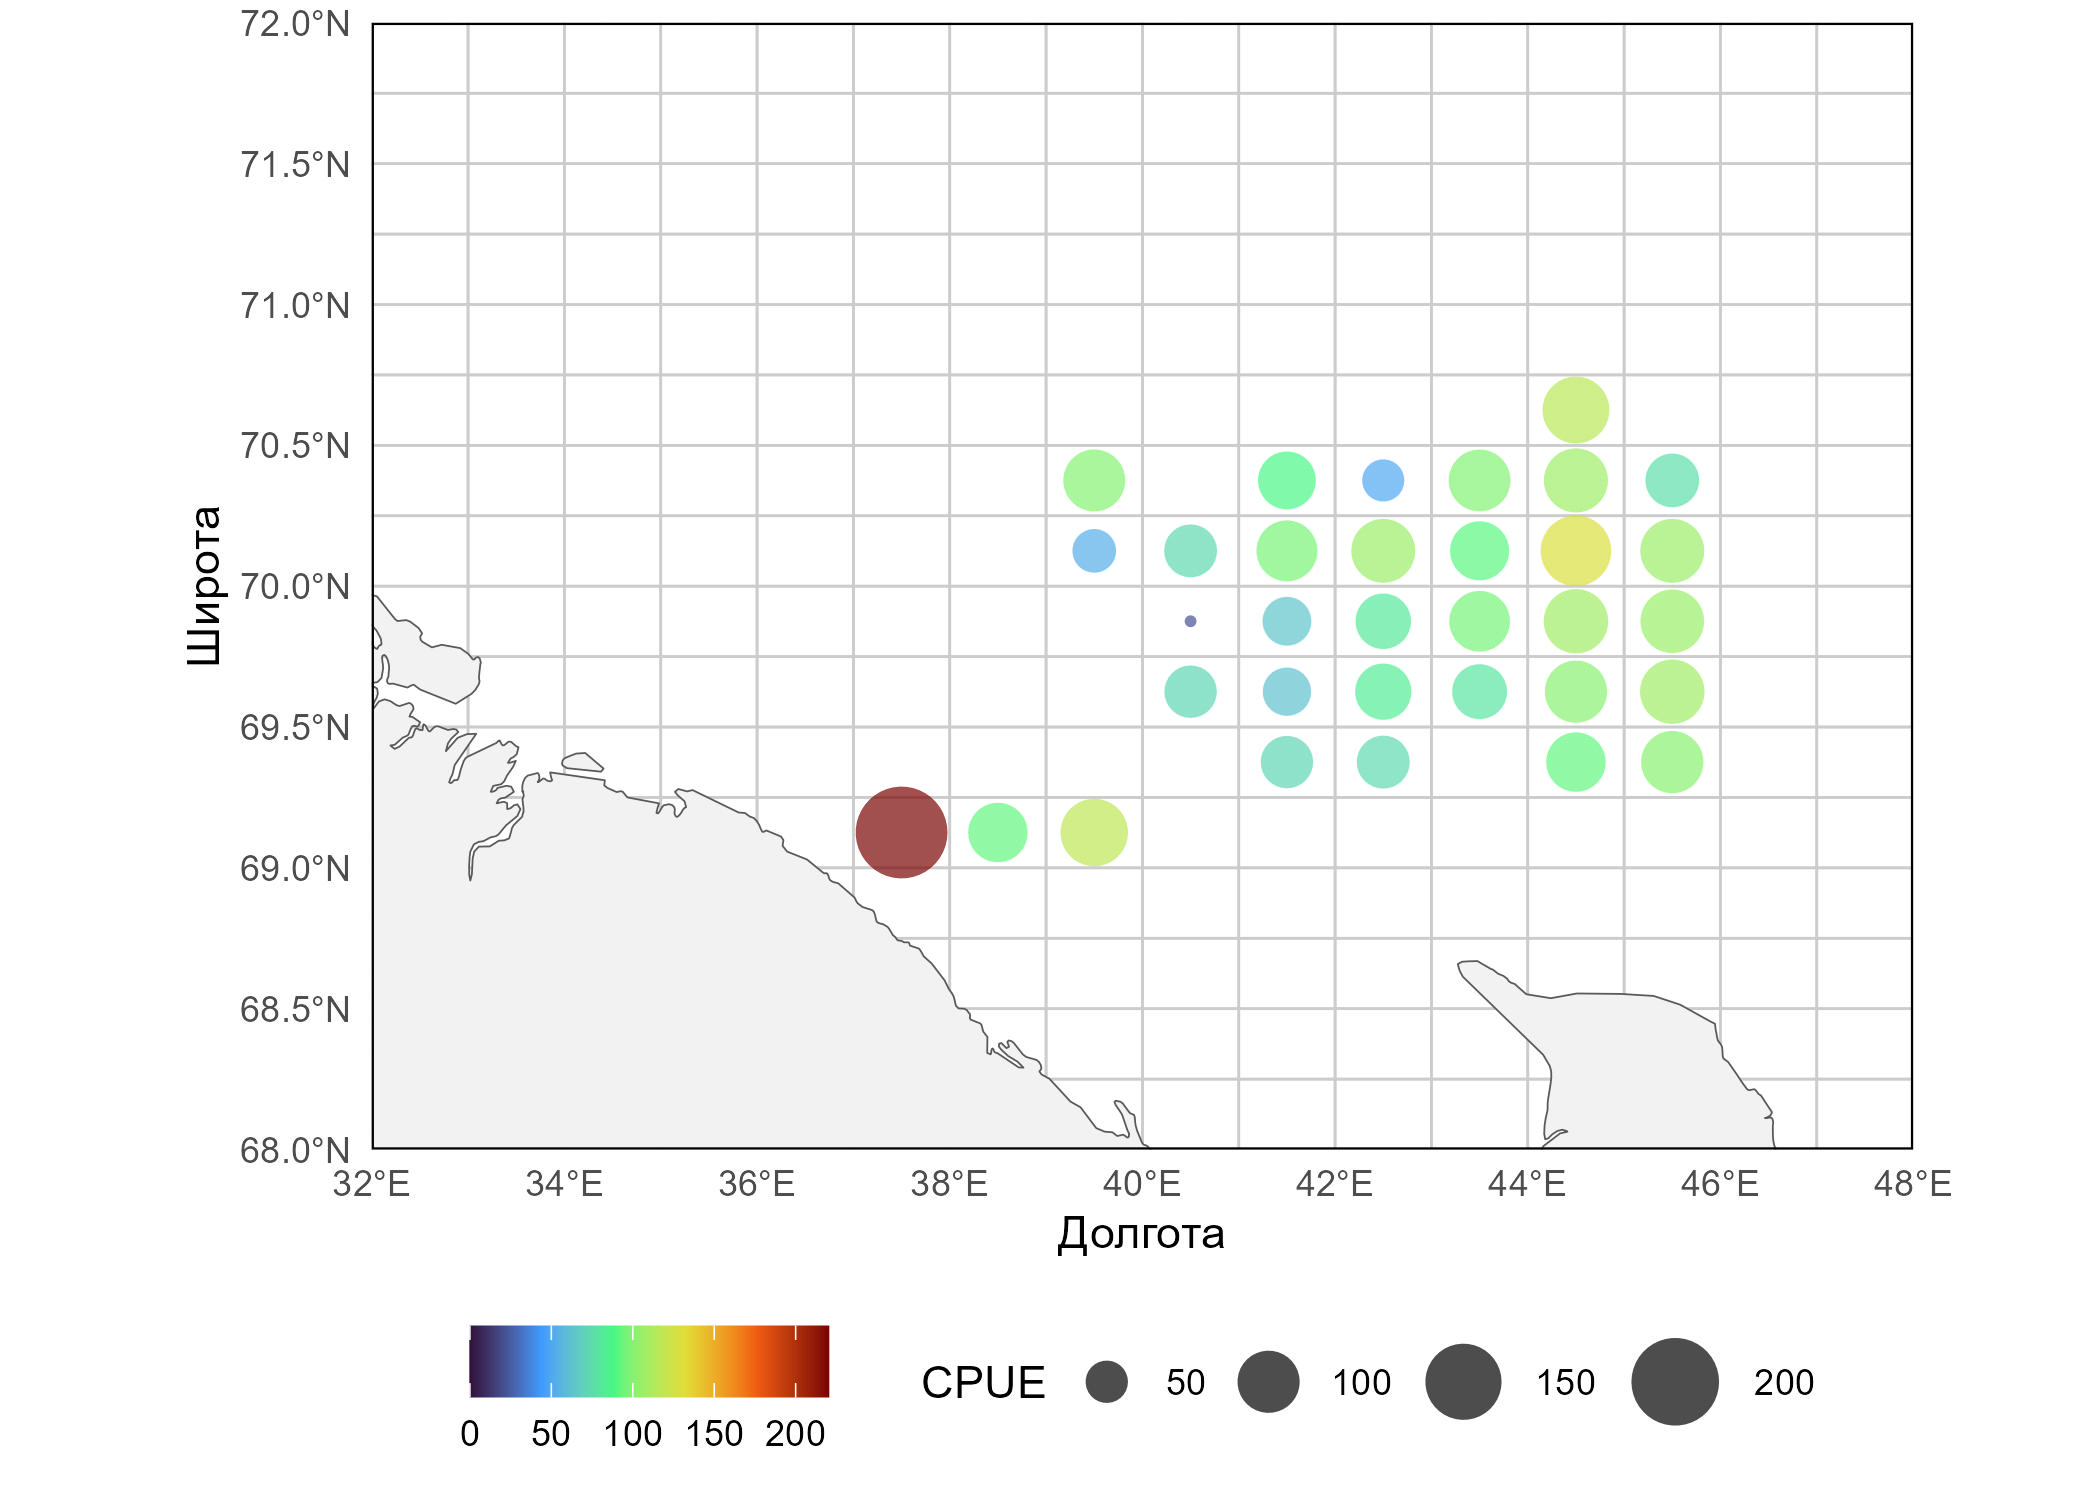
\includegraphics[width=0.8\linewidth,height=\textheight,keepaspectratio]{images/KARTOGRAPH9.jpg}

}

\caption{Рис. 9.: Промысловые карты с агрегацией в центрах полигонов
(промквадратов)}

\end{figure}%

\begin{Shaded}
\begin{Highlighting}[]
\CommentTok{\# Очистка окружения и установка рабочей директории}
\FunctionTok{rm}\NormalTok{(}\AttributeTok{list =} \FunctionTok{ls}\NormalTok{())}
\FunctionTok{setwd}\NormalTok{(}\StringTok{"C:/COURSES/KARTOGRAPH/"}\NormalTok{)}

\CommentTok{\# Загрузка необходимых библиотек}
\FunctionTok{library}\NormalTok{(rnaturalearth)}
\FunctionTok{library}\NormalTok{(tidyverse)}
\FunctionTok{library}\NormalTok{(sf)}

\DocumentationTok{\#\#\#\#\#\#\# ЗАГРУЗКА ДАННЫХ И ПОДГОТОВКА ПРОСТРАНСТВЕННЫХ ОБЪЕКТОВ \#\#\#\#\#\#\#\#\#\#\#\#\#\#\#\#}

\CommentTok{\# Чтение и фильтрация данных}
\NormalTok{DATA }\OtherTok{\textless{}{-}}\NormalTok{ readxl}\SpecialCharTok{::}\FunctionTok{read\_excel}\NormalTok{(}\StringTok{"KARTOGRAPHIC.xlsx"}\NormalTok{, }\AttributeTok{sheet =} \StringTok{"FISHERY"}\NormalTok{) }\SpecialCharTok{\%\textgreater{}\%} 
  \FunctionTok{filter}\NormalTok{(YEAR }\SpecialCharTok{==} \DecValTok{2023}\NormalTok{)}

\CommentTok{\# Преобразуем CPUE в пространственные точки}
\NormalTok{spec\_points }\OtherTok{\textless{}{-}} \FunctionTok{st\_as\_sf}\NormalTok{(DATA, }\AttributeTok{coords =} \FunctionTok{c}\NormalTok{(}\StringTok{"X"}\NormalTok{, }\StringTok{"Y"}\NormalTok{), }\AttributeTok{crs =} \DecValTok{4326}\NormalTok{)}

\CommentTok{\# Карта России}
\NormalTok{russia }\OtherTok{\textless{}{-}} \FunctionTok{ne\_countries}\NormalTok{(}\AttributeTok{scale =} \DecValTok{10}\NormalTok{, }\AttributeTok{country =} \StringTok{"Russia"}\NormalTok{) }

\CommentTok{\# Параметры карты и сетки}
\NormalTok{xmin }\OtherTok{\textless{}{-}} \DecValTok{32}\NormalTok{; xmax }\OtherTok{\textless{}{-}} \DecValTok{48}\NormalTok{; ymin }\OtherTok{\textless{}{-}} \DecValTok{68}\NormalTok{; ymax }\OtherTok{\textless{}{-}} \DecValTok{72}
\NormalTok{xcs }\OtherTok{\textless{}{-}} \DecValTok{1}\NormalTok{; ycs }\OtherTok{\textless{}{-}} \FloatTok{0.25}


\CommentTok{\# Создание основного датафрейма и пространственных объектов}
\NormalTok{points\_sf }\OtherTok{\textless{}{-}} \FunctionTok{st\_as\_sf}\NormalTok{(DATA, }\AttributeTok{coords =} \FunctionTok{c}\NormalTok{(}\StringTok{"X"}\NormalTok{, }\StringTok{"Y"}\NormalTok{), }\AttributeTok{crs =} \DecValTok{4326}\NormalTok{)}

\CommentTok{\# Создание сетки}
\NormalTok{grid\_sf }\OtherTok{\textless{}{-}} \FunctionTok{st\_make\_grid}\NormalTok{(points\_sf, }
                        \AttributeTok{cellsize =} \FunctionTok{c}\NormalTok{(xcs, ycs),}
                        \AttributeTok{n =} \FunctionTok{c}\NormalTok{(}\DecValTok{2} \SpecialCharTok{+}\NormalTok{ (xmax }\SpecialCharTok{{-}}\NormalTok{ xmin)}\SpecialCharTok{/}\NormalTok{xcs, }\DecValTok{2} \SpecialCharTok{+}\NormalTok{ (ymax }\SpecialCharTok{{-}}\NormalTok{ ymin)}\SpecialCharTok{/}\NormalTok{ycs),}
                        \AttributeTok{offset =} \FunctionTok{c}\NormalTok{(xmin }\SpecialCharTok{{-}}\NormalTok{ xcs, ymin }\SpecialCharTok{{-}}\NormalTok{ ycs)) }\SpecialCharTok{\%\textgreater{}\%} 
  \FunctionTok{st\_sf}\NormalTok{() }\SpecialCharTok{\%\textgreater{}\%} 
  \FunctionTok{mutate}\NormalTok{(}\AttributeTok{cell\_id =} \FunctionTok{row\_number}\NormalTok{())}

\CommentTok{\# Присоединяем точки Catch к сетке и агрегируем по ячейкам и годам}
\NormalTok{shares\_df\_catch }\OtherTok{\textless{}{-}} \FunctionTok{st\_join}\NormalTok{(points\_sf, grid\_sf) }\SpecialCharTok{\%\textgreater{}\%} 
  \FunctionTok{st\_drop\_geometry}\NormalTok{() }\SpecialCharTok{\%\textgreater{}\%} 
  \FunctionTok{group\_by}\NormalTok{(cell\_id, YEAR) }\SpecialCharTok{\%\textgreater{}\%} 
  \FunctionTok{summarise}\NormalTok{(}
    \AttributeTok{Count =} \FunctionTok{n}\NormalTok{(),}
    \AttributeTok{CATCH =} \FunctionTok{mean}\NormalTok{(CPUE, }\AttributeTok{na.rm =} \ConstantTok{TRUE}\NormalTok{)}
\NormalTok{  ) }\SpecialCharTok{\%\textgreater{}\%} 
  \FunctionTok{ungroup}\NormalTok{()}

\CommentTok{\# Присоединяем статистику Catch к сетке}
\NormalTok{gird\_shares\_catch }\OtherTok{\textless{}{-}} \FunctionTok{right\_join}\NormalTok{(grid\_sf, shares\_df\_catch, }\AttributeTok{by =} \StringTok{"cell\_id"}\NormalTok{)}



\CommentTok{\# Центроиды сетки по W}
\NormalTok{CENTROIDS\_W }\OtherTok{\textless{}{-}}\NormalTok{ gird\_shares\_catch }\SpecialCharTok{\%\textgreater{}\%} 
  \FunctionTok{st\_centroid}\NormalTok{()}

\DocumentationTok{\#\#\#\#\#\#\#\#\#\#\#\#\#\#\#\#\#\#\#\# ВИЗУАЛИЗАЦИЯ \#\#\#\#\#\#\#\#\#\#\#\#\#\#\#\#\#\#\#\#\#\#\#\#\#\#\#\#\#\#\#\#\#\#\#\#\#\#\#\#\#}

\FunctionTok{ggplot}\NormalTok{() }\SpecialCharTok{+}
  \CommentTok{\# 1. Сетка без заливки}
  \FunctionTok{geom\_sf}\NormalTok{(}\AttributeTok{data =}\NormalTok{ grid\_sf, }\AttributeTok{fill =} \ConstantTok{NA}\NormalTok{, }\AttributeTok{color =} \StringTok{"grey80"}\NormalTok{, }\AttributeTok{linewidth =} \FloatTok{0.3}\NormalTok{) }\SpecialCharTok{+}
  
  \CommentTok{\# 2. Границы России}
  \FunctionTok{geom\_sf}\NormalTok{(}\AttributeTok{data =}\NormalTok{ russia, }\AttributeTok{fill =} \StringTok{"grey95"}\NormalTok{) }\SpecialCharTok{+}
  
  \CommentTok{\# 3. Центроиды ячеек с CATCH (цвет и размер по значению)}
  \FunctionTok{geom\_sf}\NormalTok{(}
    \AttributeTok{data =}\NormalTok{ CENTROIDS\_W, }
    \FunctionTok{aes}\NormalTok{(}\AttributeTok{size =}\NormalTok{ CATCH, }\AttributeTok{color =}\NormalTok{ CATCH),}
    \AttributeTok{shape =} \DecValTok{16}\NormalTok{, }
    \AttributeTok{alpha =} \FloatTok{0.7}
\NormalTok{  ) }\SpecialCharTok{+}
  
  \CommentTok{\# 4. Цветовая шкала (viridis как в первом скрипте)}
  \FunctionTok{scale\_color\_viridis\_c}\NormalTok{(}
    \AttributeTok{option =} \StringTok{"H"}\NormalTok{, }
    \AttributeTok{name =} \ConstantTok{NULL}\NormalTok{,}
    \AttributeTok{limits =} \FunctionTok{c}\NormalTok{(}\DecValTok{0}\NormalTok{, }\FunctionTok{max}\NormalTok{(gird\_shares\_catch}\SpecialCharTok{$}\NormalTok{CATCH, }\AttributeTok{na.rm =} \ConstantTok{TRUE}\NormalTok{))}
\NormalTok{  ) }\SpecialCharTok{+}
  
  \CommentTok{\# 5. Шкала размера центроидов}
  \FunctionTok{scale\_size\_continuous}\NormalTok{(}
    \AttributeTok{range =} \FunctionTok{c}\NormalTok{(}\DecValTok{1}\NormalTok{, }\DecValTok{10}\NormalTok{), }
    \AttributeTok{name =} \StringTok{"CPUE"}
\NormalTok{  ) }\SpecialCharTok{+}
  
  \CommentTok{\# 6. Обрезаем область отображения}
  \FunctionTok{coord\_sf}\NormalTok{(}
    \AttributeTok{xlim =} \FunctionTok{c}\NormalTok{(xmin, xmax), }
    \AttributeTok{ylim =} \FunctionTok{c}\NormalTok{(ymin, ymax),}
    \AttributeTok{expand =} \ConstantTok{FALSE}  \CommentTok{\# Точное соответствие границ}
\NormalTok{  ) }\SpecialCharTok{+}
  
  \CommentTok{\# 7. Шкалы для осей координат}
  \FunctionTok{scale\_x\_continuous}\NormalTok{(}
    \AttributeTok{breaks =} \FunctionTok{seq}\NormalTok{(xmin, xmax, }\AttributeTok{by =} \DecValTok{2}\NormalTok{),  }\CommentTok{\# Метки каждые 2 градуса}
    \AttributeTok{name =} \StringTok{"Долгота"}
\NormalTok{  ) }\SpecialCharTok{+}
  \FunctionTok{scale\_y\_continuous}\NormalTok{(}
    \AttributeTok{breaks =} \FunctionTok{seq}\NormalTok{(ymin, ymax, }\AttributeTok{by =} \FloatTok{0.5}\NormalTok{),  }\CommentTok{\# Метки каждые 0.5 градуса}
    \AttributeTok{name =} \StringTok{"Широта"}
\NormalTok{  ) }\SpecialCharTok{+}
  
  \CommentTok{\# 8. Тема оформления}
  \FunctionTok{theme\_minimal}\NormalTok{() }\SpecialCharTok{+}
  \FunctionTok{theme}\NormalTok{(}
    \AttributeTok{panel.grid =} \FunctionTok{element\_blank}\NormalTok{(),}
    \AttributeTok{legend.position =} \StringTok{"bottom"}\NormalTok{,}
    \AttributeTok{panel.border =} \FunctionTok{element\_rect}\NormalTok{(}\AttributeTok{fill =} \ConstantTok{NA}\NormalTok{, }\AttributeTok{color =} \StringTok{"black"}\NormalTok{, }\AttributeTok{size =} \FloatTok{0.5}\NormalTok{),}
    \CommentTok{\# Добавляем сетку для осей координат}
    \AttributeTok{panel.grid.major =} \FunctionTok{element\_line}\NormalTok{(}\AttributeTok{color =} \StringTok{"gray90"}\NormalTok{, }\AttributeTok{linewidth =} \FloatTok{0.2}\NormalTok{)}
\NormalTok{  ) }\SpecialCharTok{+}
  
  \CommentTok{\# 9. Явное указание названий осей (дублируем для надежности)}
  \FunctionTok{labs}\NormalTok{(}\AttributeTok{x =} \StringTok{"Долгота"}\NormalTok{, }\AttributeTok{y =} \StringTok{"Широта"}\NormalTok{)}
\end{Highlighting}
\end{Shaded}

\section{Промысловые карты -
картограммы}\label{ux43fux440ux43eux43cux44bux441ux43bux43eux432ux44bux435-ux43aux430ux440ux442ux44b---ux43aux430ux440ux442ux43eux433ux440ux430ux43cux43cux44b}

\begin{figure}[H]

{\centering 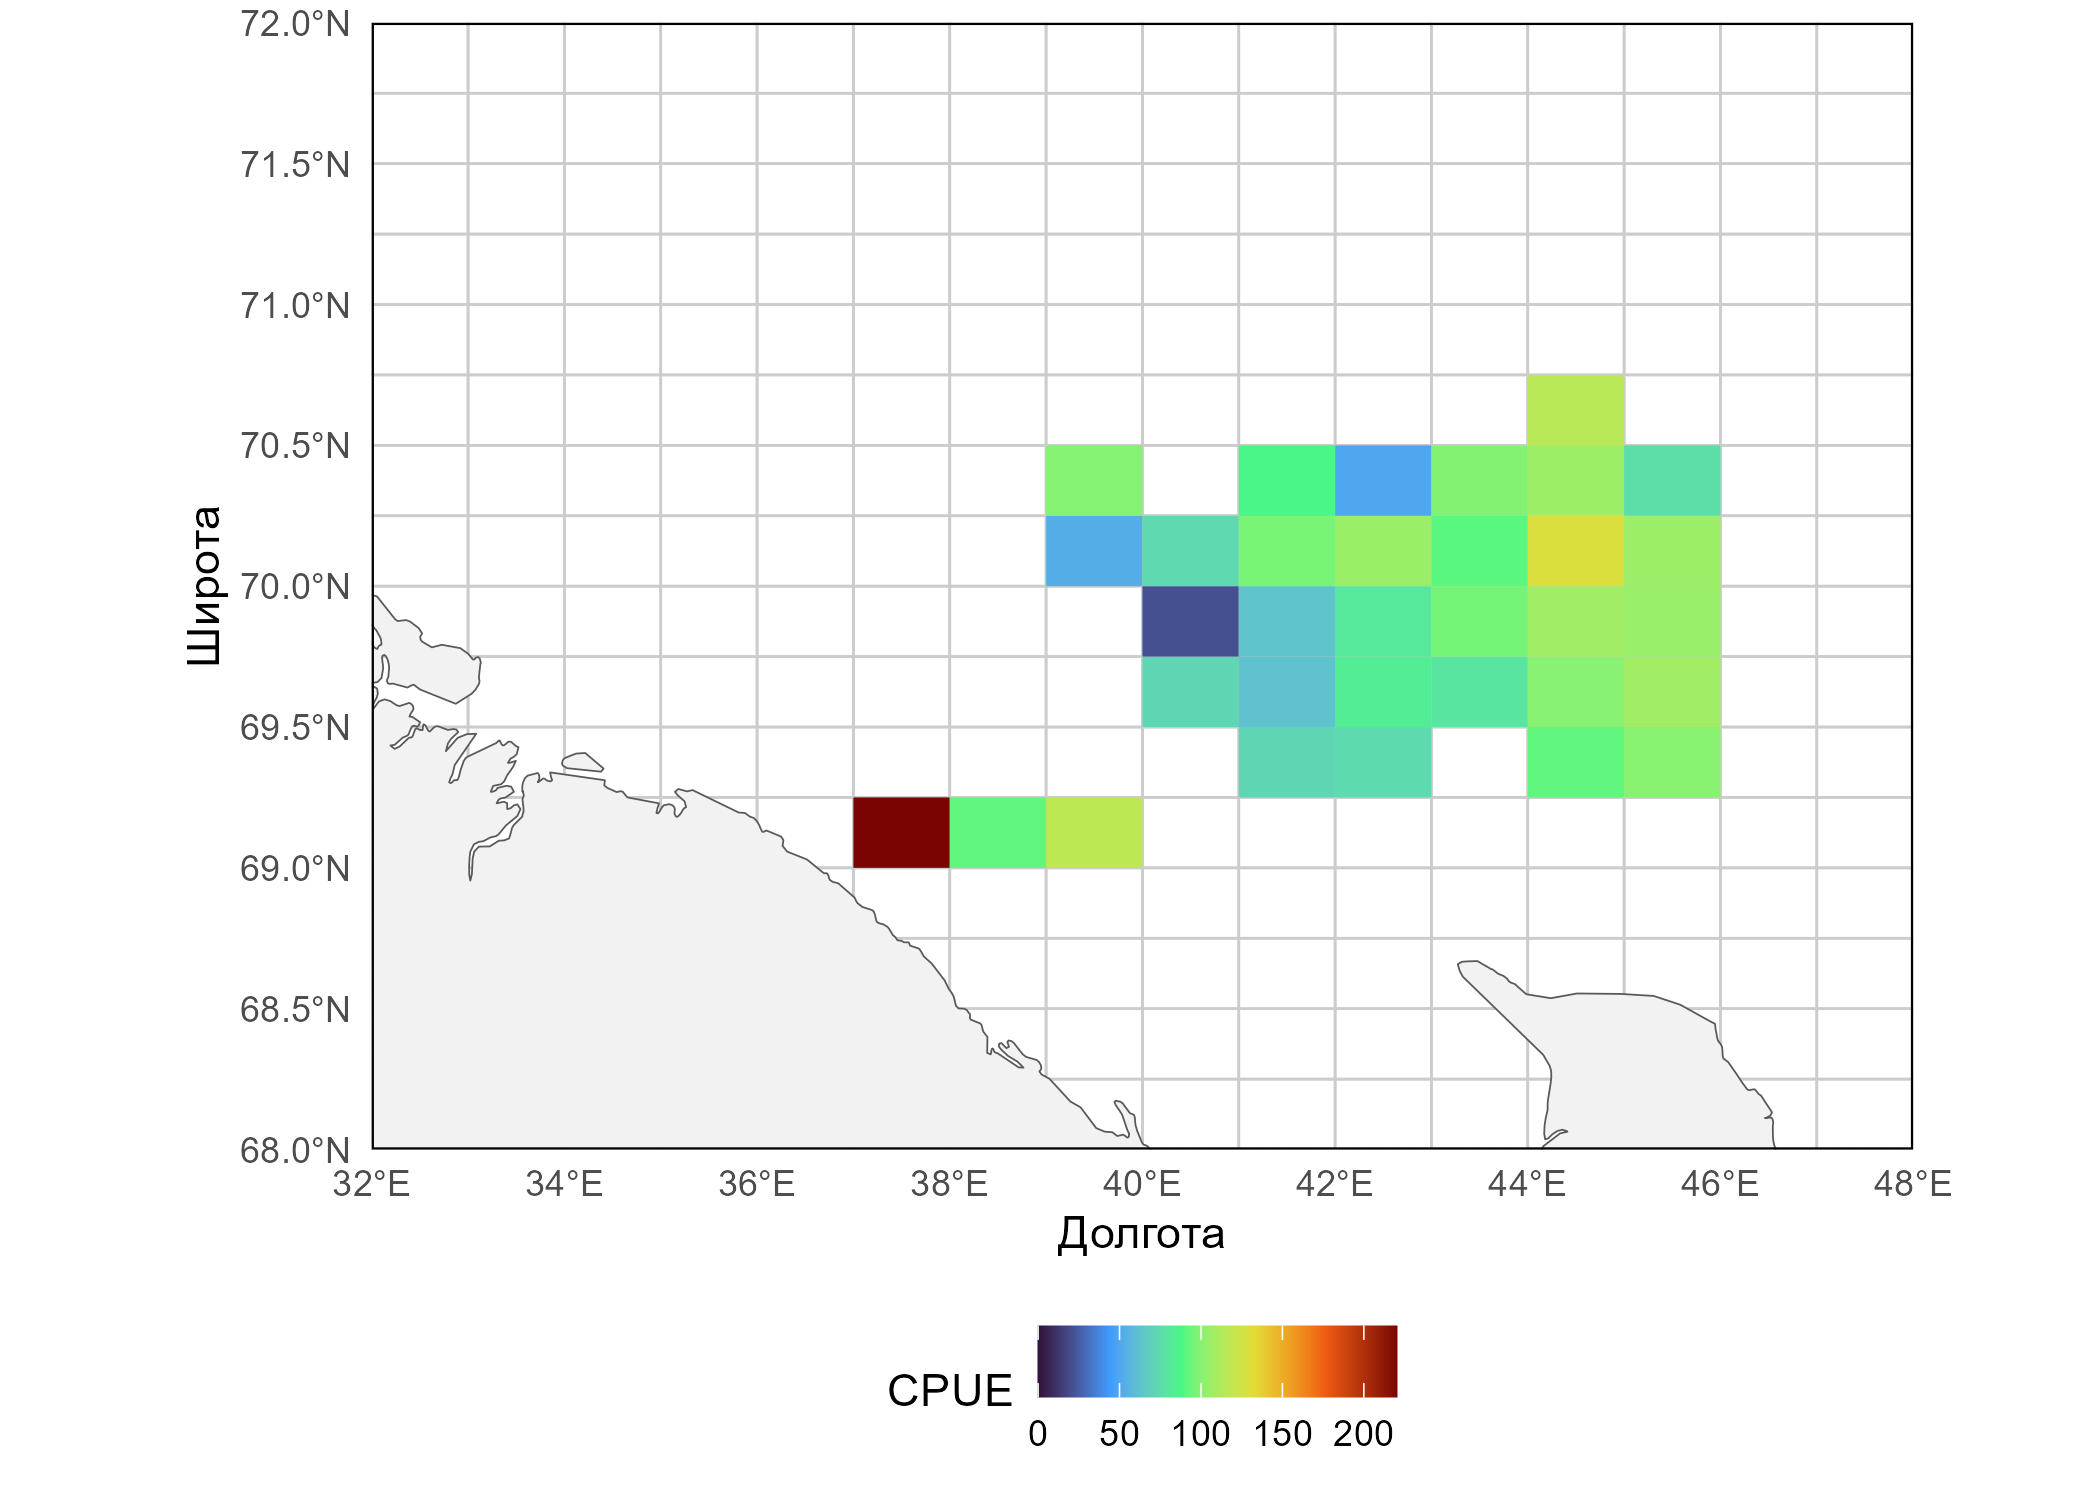
\includegraphics[width=0.8\linewidth,height=\textheight,keepaspectratio]{images/KARTOGRAPH10.jpg}

}

\caption{Рис. 10.: Промысловые карты - картограммы}

\end{figure}%

\begin{Shaded}
\begin{Highlighting}[]
\CommentTok{\# Очистка окружения и установка рабочей директории}
\FunctionTok{rm}\NormalTok{(}\AttributeTok{list =} \FunctionTok{ls}\NormalTok{())}
\FunctionTok{setwd}\NormalTok{(}\StringTok{"C:/COURSES/KARTOGRAPH/"}\NormalTok{)}

\CommentTok{\# Загрузка необходимых библиотек}
\FunctionTok{library}\NormalTok{(rnaturalearth)}
\FunctionTok{library}\NormalTok{(tidyverse)}
\FunctionTok{library}\NormalTok{(sf)}

\DocumentationTok{\#\#\#\#\#\#\# ЗАГРУЗКА ДАННЫХ И ПОДГОТОВКА ПРОСТРАНСТВЕННЫХ ОБЪЕКТОВ \#\#\#\#\#\#\#\#\#\#\#\#\#\#\#\#}

\CommentTok{\# Чтение и фильтрация данных}
\NormalTok{DATA }\OtherTok{\textless{}{-}}\NormalTok{ readxl}\SpecialCharTok{::}\FunctionTok{read\_excel}\NormalTok{(}\StringTok{"KARTOGRAPHIC.xlsx"}\NormalTok{, }\AttributeTok{sheet =} \StringTok{"FISHERY"}\NormalTok{) }\SpecialCharTok{\%\textgreater{}\%} 
  \FunctionTok{filter}\NormalTok{(YEAR }\SpecialCharTok{==} \DecValTok{2023}\NormalTok{)}

\CommentTok{\# Преобразуем CPUE в пространственные точки}
\NormalTok{spec\_points }\OtherTok{\textless{}{-}} \FunctionTok{st\_as\_sf}\NormalTok{(DATA, }\AttributeTok{coords =} \FunctionTok{c}\NormalTok{(}\StringTok{"X"}\NormalTok{, }\StringTok{"Y"}\NormalTok{), }\AttributeTok{crs =} \DecValTok{4326}\NormalTok{)}

\CommentTok{\# Карта России}
\NormalTok{russia }\OtherTok{\textless{}{-}} \FunctionTok{ne\_countries}\NormalTok{(}\AttributeTok{scale =} \DecValTok{10}\NormalTok{, }\AttributeTok{country =} \StringTok{"Russia"}\NormalTok{) }

\CommentTok{\# Параметры карты и сетки}
\NormalTok{xmin }\OtherTok{\textless{}{-}} \DecValTok{32}\NormalTok{; xmax }\OtherTok{\textless{}{-}} \DecValTok{48}\NormalTok{; ymin }\OtherTok{\textless{}{-}} \DecValTok{68}\NormalTok{; ymax }\OtherTok{\textless{}{-}} \DecValTok{72}
\NormalTok{xcs }\OtherTok{\textless{}{-}} \DecValTok{1}\NormalTok{; ycs }\OtherTok{\textless{}{-}} \FloatTok{0.25}


\CommentTok{\# Создание основного датафрейма и пространственных объектов}
\NormalTok{points\_sf }\OtherTok{\textless{}{-}} \FunctionTok{st\_as\_sf}\NormalTok{(DATA, }\AttributeTok{coords =} \FunctionTok{c}\NormalTok{(}\StringTok{"X"}\NormalTok{, }\StringTok{"Y"}\NormalTok{), }\AttributeTok{crs =} \DecValTok{4326}\NormalTok{)}

\CommentTok{\# Создание сетки}
\NormalTok{grid\_sf }\OtherTok{\textless{}{-}} \FunctionTok{st\_make\_grid}\NormalTok{(points\_sf, }
                        \AttributeTok{cellsize =} \FunctionTok{c}\NormalTok{(xcs, ycs),}
                        \AttributeTok{n =} \FunctionTok{c}\NormalTok{(}\DecValTok{2} \SpecialCharTok{+}\NormalTok{ (xmax }\SpecialCharTok{{-}}\NormalTok{ xmin)}\SpecialCharTok{/}\NormalTok{xcs, }\DecValTok{2} \SpecialCharTok{+}\NormalTok{ (ymax }\SpecialCharTok{{-}}\NormalTok{ ymin)}\SpecialCharTok{/}\NormalTok{ycs),}
                        \AttributeTok{offset =} \FunctionTok{c}\NormalTok{(xmin }\SpecialCharTok{{-}}\NormalTok{ xcs, ymin }\SpecialCharTok{{-}}\NormalTok{ ycs)) }\SpecialCharTok{\%\textgreater{}\%} 
  \FunctionTok{st\_sf}\NormalTok{() }\SpecialCharTok{\%\textgreater{}\%} 
  \FunctionTok{mutate}\NormalTok{(}\AttributeTok{cell\_id =} \FunctionTok{row\_number}\NormalTok{())}

\CommentTok{\# Присоединяем точки Catch к сетке и агрегируем по ячейкам и годам}
\NormalTok{shares\_df\_catch }\OtherTok{\textless{}{-}} \FunctionTok{st\_join}\NormalTok{(points\_sf, grid\_sf) }\SpecialCharTok{\%\textgreater{}\%} 
  \FunctionTok{st\_drop\_geometry}\NormalTok{() }\SpecialCharTok{\%\textgreater{}\%} 
  \FunctionTok{group\_by}\NormalTok{(cell\_id, YEAR) }\SpecialCharTok{\%\textgreater{}\%} 
  \FunctionTok{summarise}\NormalTok{(}
    \AttributeTok{Count =} \FunctionTok{n}\NormalTok{(),}
    \AttributeTok{CATCH =} \FunctionTok{mean}\NormalTok{(CPUE, }\AttributeTok{na.rm =} \ConstantTok{TRUE}\NormalTok{)}
\NormalTok{  ) }\SpecialCharTok{\%\textgreater{}\%} 
  \FunctionTok{ungroup}\NormalTok{()}

\CommentTok{\# Присоединяем статистику Catch к сетке}
\NormalTok{gird\_shares\_catch }\OtherTok{\textless{}{-}} \FunctionTok{right\_join}\NormalTok{(grid\_sf, shares\_df\_catch, }\AttributeTok{by =} \StringTok{"cell\_id"}\NormalTok{)}



\CommentTok{\# Центроиды сетки по W}
\NormalTok{CENTROIDS\_W }\OtherTok{\textless{}{-}}\NormalTok{ gird\_shares\_catch }\SpecialCharTok{\%\textgreater{}\%} 
  \FunctionTok{st\_centroid}\NormalTok{()}

\DocumentationTok{\#\#\#\#\#\#\#\#\#\#\#\#\#\#\#\#\#\#\#\# ВИЗУАЛИЗАЦИЯ \#\#\#\#\#\#\#\#\#\#\#\#\#\#\#\#\#\#\#\#\#\#\#\#\#\#\#\#\#\#\#\#\#\#\#\#\#\#\#\#\#}

\FunctionTok{ggplot}\NormalTok{() }\SpecialCharTok{+}
  \CommentTok{\# 1. Сетка без заливки}
  \FunctionTok{geom\_sf}\NormalTok{(}\AttributeTok{data =}\NormalTok{ grid\_sf, }\AttributeTok{fill =} \ConstantTok{NA}\NormalTok{, }\AttributeTok{color =} \StringTok{"grey80"}\NormalTok{, }\AttributeTok{linewidth =} \FloatTok{0.3}\NormalTok{) }\SpecialCharTok{+}
  
  \CommentTok{\# 2. Границы России}
  \FunctionTok{geom\_sf}\NormalTok{(}\AttributeTok{data =}\NormalTok{ russia, }\AttributeTok{fill =} \StringTok{"grey95"}\NormalTok{) }\SpecialCharTok{+}
  
  \CommentTok{\# 3. Заливка по улову с палитрой viridis option "H"}
  \FunctionTok{geom\_sf}\NormalTok{(}\AttributeTok{data =}\NormalTok{ gird\_shares\_catch, }\FunctionTok{aes}\NormalTok{(}\AttributeTok{fill =}\NormalTok{ CATCH), }\AttributeTok{color =} \ConstantTok{NA}\NormalTok{) }\SpecialCharTok{+}
  
  \CommentTok{\# 4. Цветовая шкала viridis option "H" для заливки}
  \FunctionTok{scale\_fill\_viridis\_c}\NormalTok{(}
    \AttributeTok{option =} \StringTok{"H"}\NormalTok{, }
    \AttributeTok{name =} \StringTok{"CPUE"}\NormalTok{,}
    \AttributeTok{limits =} \FunctionTok{c}\NormalTok{(}\DecValTok{0}\NormalTok{, }\FunctionTok{max}\NormalTok{(gird\_shares\_catch}\SpecialCharTok{$}\NormalTok{CATCH, }\AttributeTok{na.rm =} \ConstantTok{TRUE}\NormalTok{)),}
    \AttributeTok{na.value =} \StringTok{"transparent"}
\NormalTok{  ) }\SpecialCharTok{+}
  
  \CommentTok{\# 5. Обрезаем область отображения}
  \FunctionTok{coord\_sf}\NormalTok{(}
    \AttributeTok{xlim =} \FunctionTok{c}\NormalTok{(xmin, xmax), }
    \AttributeTok{ylim =} \FunctionTok{c}\NormalTok{(ymin, ymax),}
    \AttributeTok{expand =} \ConstantTok{FALSE}
\NormalTok{  ) }\SpecialCharTok{+}
  
  \CommentTok{\# 6. Шкалы для осей координат}
  \FunctionTok{scale\_x\_continuous}\NormalTok{(}
    \AttributeTok{breaks =} \FunctionTok{seq}\NormalTok{(xmin, xmax, }\AttributeTok{by =} \DecValTok{2}\NormalTok{),}
    \AttributeTok{name =} \StringTok{"Долгота"}
\NormalTok{  ) }\SpecialCharTok{+}
  \FunctionTok{scale\_y\_continuous}\NormalTok{(}
    \AttributeTok{breaks =} \FunctionTok{seq}\NormalTok{(ymin, ymax, }\AttributeTok{by =} \FloatTok{0.5}\NormalTok{),}
    \AttributeTok{name =} \StringTok{"Широта"}
\NormalTok{  ) }\SpecialCharTok{+}
  
  \CommentTok{\# 7. Тема оформления}
  \FunctionTok{theme\_minimal}\NormalTok{() }\SpecialCharTok{+}
  \FunctionTok{theme}\NormalTok{(}
    \AttributeTok{panel.grid =} \FunctionTok{element\_blank}\NormalTok{(),}
    \AttributeTok{legend.position =} \StringTok{"bottom"}\NormalTok{,}
    \AttributeTok{panel.border =} \FunctionTok{element\_rect}\NormalTok{(}\AttributeTok{fill =} \ConstantTok{NA}\NormalTok{, }\AttributeTok{color =} \StringTok{"black"}\NormalTok{, }\AttributeTok{size =} \FloatTok{0.5}\NormalTok{),}
    \AttributeTok{panel.grid.major =} \FunctionTok{element\_line}\NormalTok{(}\AttributeTok{color =} \StringTok{"gray90"}\NormalTok{, }\AttributeTok{size =} \FloatTok{0.2}\NormalTok{)}
\NormalTok{  ) }\SpecialCharTok{+}
  \FunctionTok{labs}\NormalTok{(}\AttributeTok{x =} \StringTok{"Долгота"}\NormalTok{, }\AttributeTok{y =} \StringTok{"Широта"}\NormalTok{)}
\end{Highlighting}
\end{Shaded}

\section{Промысловые карты - картограммы по
фасеткам}\label{ux43fux440ux43eux43cux44bux441ux43bux43eux432ux44bux435-ux43aux430ux440ux442ux44b---ux43aux430ux440ux442ux43eux433ux440ux430ux43cux43cux44b-ux43fux43e-ux444ux430ux441ux435ux442ux43aux430ux43c}

\begin{figure}[H]

{\centering 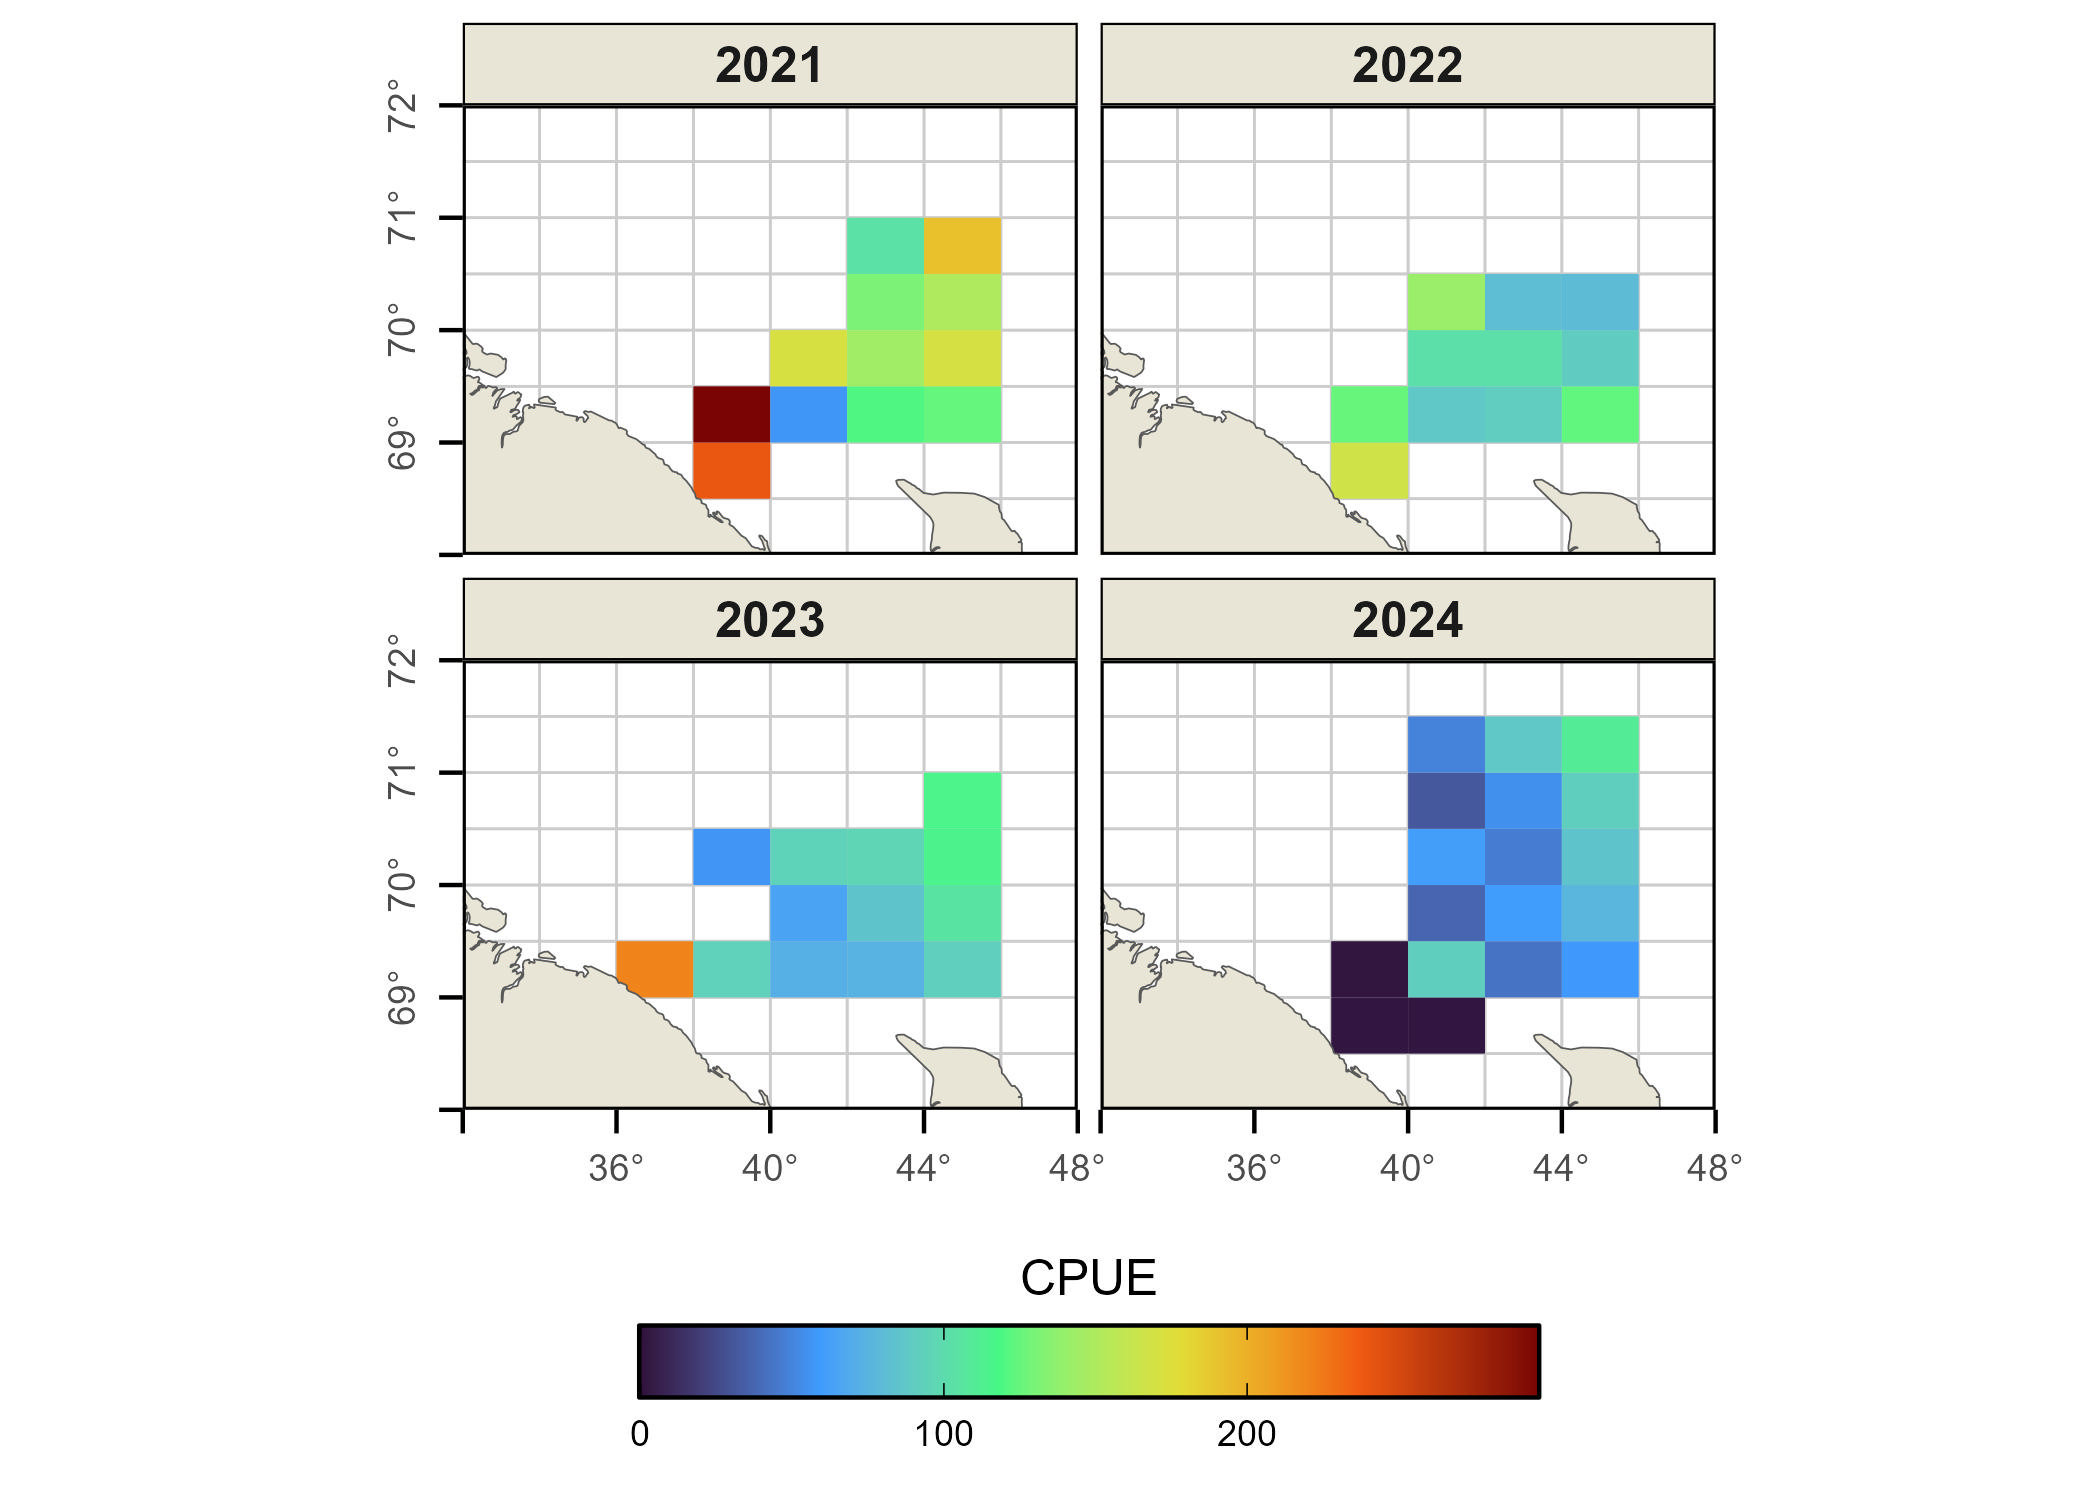
\includegraphics[width=0.8\linewidth,height=\textheight,keepaspectratio]{images/KARTOGRAPH11.jpg}

}

\caption{Рис. 11.: Промысловые карты - картограммы по фасеткам}

\end{figure}%

\begin{Shaded}
\begin{Highlighting}[]
\CommentTok{\# Очистка окружения и установка рабочей директории}
\FunctionTok{rm}\NormalTok{(}\AttributeTok{list =} \FunctionTok{ls}\NormalTok{())}
\FunctionTok{setwd}\NormalTok{(}\StringTok{"C:/COURSES/KARTOGRAPH/"}\NormalTok{)}

\FunctionTok{library}\NormalTok{(rnaturalearth)}
\FunctionTok{library}\NormalTok{(tidyverse)}
\FunctionTok{library}\NormalTok{(ggspatial)}
\FunctionTok{library}\NormalTok{(sf)}

\DocumentationTok{\#\#\#\#\#\#\# READ DATA AND PREPARE SPATIAL OBJECTS \#\#\#\#\#\#\#\#\#\#\#\#\#\#\#\#\#\#\#\#\#\#\#\#\#\#\#\#}

\CommentTok{\# Чтение и фильтрация данных}
\NormalTok{DATA }\OtherTok{\textless{}{-}}\NormalTok{ readxl}\SpecialCharTok{::}\FunctionTok{read\_excel}\NormalTok{(}\StringTok{"KARTOGRAPHIC.xlsx"}\NormalTok{, }\AttributeTok{sheet =} \StringTok{"FISHERY"}\NormalTok{) }\SpecialCharTok{\%\textgreater{}\%} 
  \FunctionTok{filter}\NormalTok{(YEAR }\SpecialCharTok{\textgreater{}} \DecValTok{2020} \SpecialCharTok{\&}\NormalTok{ YEAR }\SpecialCharTok{\textless{}} \DecValTok{2025}\NormalTok{)}

\CommentTok{\# Карта России}
\NormalTok{russia }\OtherTok{\textless{}{-}} \FunctionTok{ne\_countries}\NormalTok{(}\AttributeTok{scale =} \DecValTok{10}\NormalTok{, }\AttributeTok{country =} \StringTok{"Russia"}\NormalTok{) }

\CommentTok{\# Параметры карты и сетки}
\NormalTok{xmin }\OtherTok{\textless{}{-}} \DecValTok{32}\NormalTok{; xmax }\OtherTok{\textless{}{-}} \DecValTok{48}\NormalTok{; ymin }\OtherTok{\textless{}{-}} \DecValTok{68}\NormalTok{; ymax }\OtherTok{\textless{}{-}} \DecValTok{72}
\NormalTok{xcs }\OtherTok{\textless{}{-}} \DecValTok{2}\NormalTok{; ycs }\OtherTok{\textless{}{-}} \FloatTok{0.5}

\CommentTok{\# Преобразование в пространственные объекты}
\NormalTok{points\_sf }\OtherTok{\textless{}{-}} \FunctionTok{st\_as\_sf}\NormalTok{(DATA, }\AttributeTok{coords =} \FunctionTok{c}\NormalTok{(}\StringTok{"X"}\NormalTok{, }\StringTok{"Y"}\NormalTok{), }\AttributeTok{crs =} \DecValTok{4326}\NormalTok{)}

\CommentTok{\# Создание сетки}
\NormalTok{grid\_sf }\OtherTok{\textless{}{-}} \FunctionTok{st\_make\_grid}\NormalTok{(}
\NormalTok{  points\_sf,}
  \AttributeTok{cellsize =} \FunctionTok{c}\NormalTok{(xcs, ycs),}
  \AttributeTok{n =} \FunctionTok{c}\NormalTok{(}\DecValTok{2} \SpecialCharTok{+}\NormalTok{ (xmax }\SpecialCharTok{{-}}\NormalTok{ xmin)}\SpecialCharTok{/}\NormalTok{xcs, }\DecValTok{2} \SpecialCharTok{+}\NormalTok{ (ymax }\SpecialCharTok{{-}}\NormalTok{ ymin)}\SpecialCharTok{/}\NormalTok{ycs),}
  \AttributeTok{offset =} \FunctionTok{c}\NormalTok{(xmin }\SpecialCharTok{{-}}\NormalTok{ xcs, ymin }\SpecialCharTok{{-}}\NormalTok{ ycs)}
\NormalTok{) }\SpecialCharTok{\%\textgreater{}\%} 
  \FunctionTok{st\_sf}\NormalTok{() }\SpecialCharTok{\%\textgreater{}\%} 
  \FunctionTok{mutate}\NormalTok{(}\AttributeTok{cell\_id =} \FunctionTok{row\_number}\NormalTok{())}

\CommentTok{\# Агрегация данных по сетке и годам}
\NormalTok{shares\_df\_catch }\OtherTok{\textless{}{-}}\NormalTok{ points\_sf }\SpecialCharTok{\%\textgreater{}\%} 
  \FunctionTok{st\_join}\NormalTok{(grid\_sf) }\SpecialCharTok{\%\textgreater{}\%} 
  \FunctionTok{st\_drop\_geometry}\NormalTok{() }\SpecialCharTok{\%\textgreater{}\%} 
  \FunctionTok{group\_by}\NormalTok{(cell\_id, YEAR) }\SpecialCharTok{\%\textgreater{}\%} 
  \FunctionTok{summarise}\NormalTok{(}\AttributeTok{CATCH =} \FunctionTok{mean}\NormalTok{(CPUE, }\AttributeTok{na.rm =} \ConstantTok{TRUE}\NormalTok{), }\AttributeTok{.groups =} \StringTok{\textquotesingle{}drop\textquotesingle{}}\NormalTok{)}

\CommentTok{\# Присоединение статистики к сетке}
\NormalTok{gird\_shares\_catch }\OtherTok{\textless{}{-}}\NormalTok{ grid\_sf }\SpecialCharTok{\%\textgreater{}\%} 
  \FunctionTok{right\_join}\NormalTok{(shares\_df\_catch, }\AttributeTok{by =} \StringTok{"cell\_id"}\NormalTok{)}

\DocumentationTok{\#\#\#\#\#\#\#\#\#\#\#\#\#\#\#\#\#\#\#\# ВИЗУАЛИЗАЦИЯ \#\#\#\#\#\#\#\#\#\#\#\#\#\#\#\#\#\#\#\#\#\#\#\#\#\#\#\#\#\#\#\#\#\#\#\#\#\#\#\#\#}

\CommentTok{\# Определяем общий максимум CPUE для единой шкалы цветов}
\NormalTok{catch\_max }\OtherTok{\textless{}{-}} \FunctionTok{max}\NormalTok{(gird\_shares\_catch}\SpecialCharTok{$}\NormalTok{CATCH, }\AttributeTok{na.rm =} \ConstantTok{TRUE}\NormalTok{)}

\CommentTok{\# Рассчитываем шаг для подписей (в 2 раза реже исходной сетки)}
\NormalTok{x\_breaks }\OtherTok{\textless{}{-}} \FunctionTok{seq}\NormalTok{(xmin, xmax, }\AttributeTok{by =}\NormalTok{ xcs }\SpecialCharTok{*} \DecValTok{2}\NormalTok{)  }\CommentTok{\# 4 градуса}
\NormalTok{y\_breaks }\OtherTok{\textless{}{-}} \FunctionTok{seq}\NormalTok{(ymin, ymax, }\AttributeTok{by =}\NormalTok{ ycs }\SpecialCharTok{*} \DecValTok{2}\NormalTok{)  }\CommentTok{\# 1 градус}

\CommentTok{\# Функция для форматирования подписей: пропускаем первую подпись}
\NormalTok{format\_labels }\OtherTok{\textless{}{-}} \ControlFlowTok{function}\NormalTok{(breaks) \{}
\NormalTok{  labels }\OtherTok{\textless{}{-}} \FunctionTok{paste0}\NormalTok{(breaks, }\StringTok{"°"}\NormalTok{)}
\NormalTok{  labels[}\DecValTok{1}\NormalTok{] }\OtherTok{\textless{}{-}} \StringTok{""}  \CommentTok{\# Пропускаем первую подпись}
  \FunctionTok{return}\NormalTok{(labels)}
\NormalTok{\}}

\FunctionTok{ggplot}\NormalTok{() }\SpecialCharTok{+}
  \CommentTok{\# Контуры сетки}
  \FunctionTok{geom\_sf}\NormalTok{(}\AttributeTok{data =}\NormalTok{ grid\_sf, }\AttributeTok{fill =} \ConstantTok{NA}\NormalTok{, }\AttributeTok{color =} \StringTok{"grey80"}\NormalTok{, }\AttributeTok{linewidth =} \FloatTok{0.3}\NormalTok{) }\SpecialCharTok{+}
  
  \CommentTok{\# Заливка по улову с цветовой схемой viridis}
  \FunctionTok{geom\_sf}\NormalTok{(}\AttributeTok{data =}\NormalTok{ gird\_shares\_catch, }\FunctionTok{aes}\NormalTok{(}\AttributeTok{fill =}\NormalTok{ CATCH), }\AttributeTok{color =} \ConstantTok{NA}\NormalTok{) }\SpecialCharTok{+}
  
  \CommentTok{\# Границы России}
  \FunctionTok{geom\_sf}\NormalTok{(}\AttributeTok{data =}\NormalTok{ russia, }\AttributeTok{fill =} \StringTok{"\#E8E5D6"}\NormalTok{) }\SpecialCharTok{+}
  
  \CommentTok{\# Фасетирование по годам}
  \FunctionTok{facet\_wrap}\NormalTok{(}\SpecialCharTok{\textasciitilde{}}\NormalTok{ YEAR, }\AttributeTok{nrow =} \DecValTok{2}\NormalTok{) }\SpecialCharTok{+}
  
  \CommentTok{\# Цветовая шкала}
  \FunctionTok{scale\_fill\_viridis\_c}\NormalTok{(}
    \AttributeTok{option =} \StringTok{"H"}\NormalTok{, }
    \AttributeTok{name =} \StringTok{"CPUE"}\NormalTok{,}
    \AttributeTok{limits =} \FunctionTok{c}\NormalTok{(}\DecValTok{0}\NormalTok{, catch\_max),}
    \AttributeTok{na.value =} \StringTok{"transparent"}
\NormalTok{  ) }\SpecialCharTok{+}
  
  \CommentTok{\# Область отображения}
  \FunctionTok{coord\_sf}\NormalTok{(}
    \AttributeTok{xlim =} \FunctionTok{c}\NormalTok{(xmin, xmax), }
    \AttributeTok{ylim =} \FunctionTok{c}\NormalTok{(ymin, ymax),}
    \AttributeTok{expand =} \ConstantTok{FALSE}
\NormalTok{  ) }\SpecialCharTok{+}
  
  \CommentTok{\# Управление подписями осей с символом градуса (пропускаем первую подпись)}
  \FunctionTok{scale\_x\_continuous}\NormalTok{(}
    \AttributeTok{breaks =}\NormalTok{ x\_breaks,}
    \AttributeTok{labels =}\NormalTok{ format\_labels}
\NormalTok{  ) }\SpecialCharTok{+}
  \FunctionTok{scale\_y\_continuous}\NormalTok{(}
    \AttributeTok{breaks =}\NormalTok{ y\_breaks,}
    \AttributeTok{labels =}\NormalTok{ format\_labels}
\NormalTok{  ) }\SpecialCharTok{+}
  
  \CommentTok{\# Оформление с тиками на осях}
  \FunctionTok{theme\_minimal}\NormalTok{() }\SpecialCharTok{+}
  \FunctionTok{theme}\NormalTok{(}
    \AttributeTok{panel.grid =} \FunctionTok{element\_blank}\NormalTok{(),}
    \AttributeTok{legend.position =} \StringTok{"bottom"}\NormalTok{,}
    \AttributeTok{legend.key.width =} \FunctionTok{unit}\NormalTok{(}\FloatTok{2.5}\NormalTok{, }\StringTok{"cm"}\NormalTok{),}
    \AttributeTok{legend.title =} \FunctionTok{element\_text}\NormalTok{(}\AttributeTok{vjust =} \FloatTok{0.8}\NormalTok{, }\AttributeTok{size =} \DecValTok{12}\NormalTok{),}
    \AttributeTok{panel.border =} \FunctionTok{element\_rect}\NormalTok{(}\AttributeTok{fill =} \ConstantTok{NA}\NormalTok{, }\AttributeTok{color =} \StringTok{"black"}\NormalTok{, }\AttributeTok{size =} \FloatTok{0.7}\NormalTok{),}
    \AttributeTok{panel.grid.major =} \FunctionTok{element\_line}\NormalTok{(}\AttributeTok{color =} \StringTok{"grey90"}\NormalTok{, }\AttributeTok{size =} \FloatTok{0.2}\NormalTok{),}
    \AttributeTok{strip.background =} \FunctionTok{element\_rect}\NormalTok{(}\AttributeTok{fill =} \StringTok{"\#E8E5D6"}\NormalTok{, }\AttributeTok{color =} \StringTok{"black"}\NormalTok{),}
    \AttributeTok{strip.text =} \FunctionTok{element\_text}\NormalTok{(}\AttributeTok{face =} \StringTok{"bold"}\NormalTok{, }\AttributeTok{size =} \DecValTok{12}\NormalTok{),}
    \AttributeTok{axis.text.x =} \FunctionTok{element\_text}\NormalTok{(}\AttributeTok{size =} \DecValTok{9}\NormalTok{, }\AttributeTok{angle =} \DecValTok{0}\NormalTok{, }\AttributeTok{margin =} \FunctionTok{margin}\NormalTok{(}\AttributeTok{t =} \DecValTok{5}\NormalTok{)),}
    \AttributeTok{axis.text.y =} \FunctionTok{element\_text}\NormalTok{(}\AttributeTok{size =} \DecValTok{9}\NormalTok{, }\AttributeTok{angle =} \DecValTok{90}\NormalTok{, }\AttributeTok{hjust =} \FloatTok{0.5}\NormalTok{, }\AttributeTok{margin =} \FunctionTok{margin}\NormalTok{(}\AttributeTok{r =} \DecValTok{5}\NormalTok{)),}
    \AttributeTok{axis.title.x =} \FunctionTok{element\_blank}\NormalTok{(),}
    \AttributeTok{axis.title.y =} \FunctionTok{element\_blank}\NormalTok{(),}
    
    \CommentTok{\# Тики (засечки) на оси}
    \AttributeTok{axis.ticks =} \FunctionTok{element\_line}\NormalTok{(}\AttributeTok{color =} \StringTok{"black"}\NormalTok{, }\AttributeTok{size =} \FloatTok{0.5}\NormalTok{),}
    \AttributeTok{axis.ticks.length =} \FunctionTok{unit}\NormalTok{(}\FloatTok{0.2}\NormalTok{, }\StringTok{"cm"}\NormalTok{),}
    \AttributeTok{axis.ticks.x =} \FunctionTok{element\_line}\NormalTok{(}\AttributeTok{color =} \StringTok{"black"}\NormalTok{, }\AttributeTok{size =} \FloatTok{0.5}\NormalTok{),}
    \AttributeTok{axis.ticks.y =} \FunctionTok{element\_line}\NormalTok{(}\AttributeTok{color =} \StringTok{"black"}\NormalTok{, }\AttributeTok{size =} \FloatTok{0.5}\NormalTok{)}
\NormalTok{  ) }\SpecialCharTok{+}
  
  \CommentTok{\# Настройка легенды}
  \FunctionTok{guides}\NormalTok{(}\AttributeTok{fill =} \FunctionTok{guide\_colorbar}\NormalTok{(}
    \AttributeTok{title.position =} \StringTok{"top"}\NormalTok{,}
    \AttributeTok{title.hjust =} \FloatTok{0.5}\NormalTok{,}
    \AttributeTok{barwidth =} \DecValTok{15}\NormalTok{,}
    \AttributeTok{frame.colour =} \StringTok{"black"}\NormalTok{,}
    \AttributeTok{ticks.colour =} \StringTok{"black"}
\NormalTok{  ))}

\CommentTok{\# Сохранение результата}
\FunctionTok{ggsave}\NormalTok{(}\StringTok{"KARTOGRAPH11.jpg"}\NormalTok{, }
       \AttributeTok{device =} \StringTok{"jpeg"}\NormalTok{, }
       \AttributeTok{dpi =} \DecValTok{300}\NormalTok{,}
       \AttributeTok{width =} \DecValTok{7}\NormalTok{,}
       \AttributeTok{height =} \DecValTok{5}\NormalTok{,}
       \AttributeTok{units =} \StringTok{"in"}\NormalTok{)}
\end{Highlighting}
\end{Shaded}

\section{Гибридные карты - картограммы и точки (съемка и промысловые
данные)}\label{ux433ux438ux431ux440ux438ux434ux43dux44bux435-ux43aux430ux440ux442ux44b---ux43aux430ux440ux442ux43eux433ux440ux430ux43cux43cux44b-ux438-ux442ux43eux447ux43aux438-ux441ux44aux435ux43cux43aux430-ux438-ux43fux440ux43eux43cux44bux441ux43bux43eux432ux44bux435-ux434ux430ux43dux43dux44bux435}

\begin{figure}[H]

{\centering 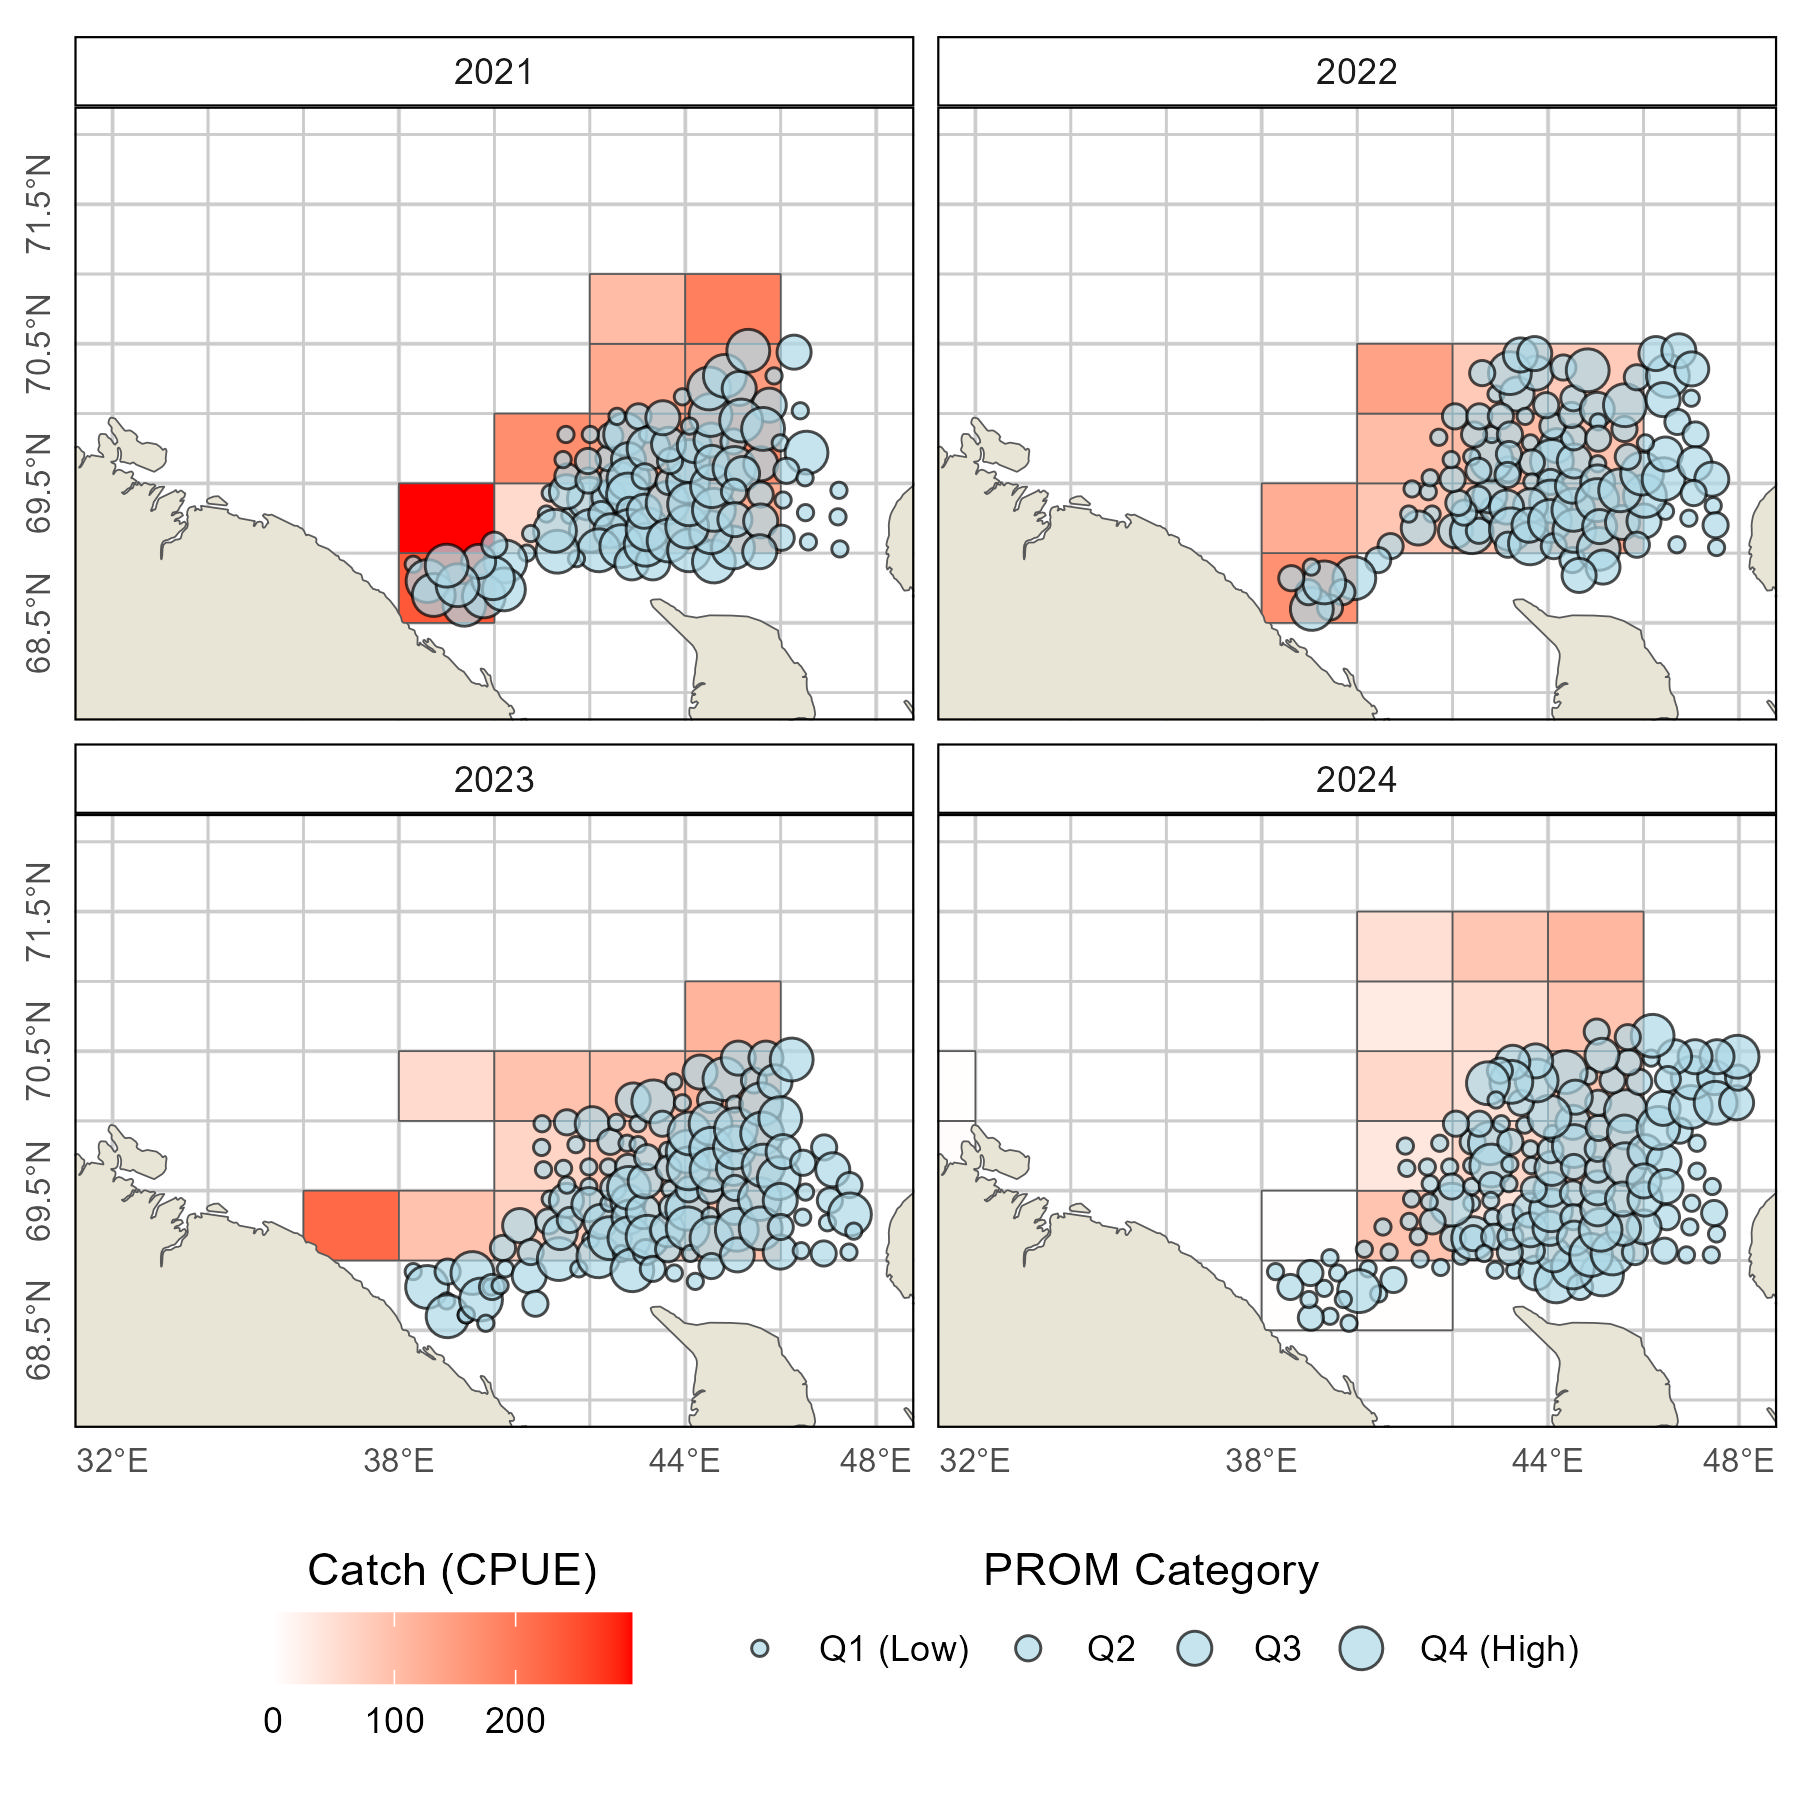
\includegraphics[width=0.8\linewidth,height=\textheight,keepaspectratio]{images/KARTOGRAPH12.jpg}

}

\caption{Рис. 12.: Гибридные карты - картограммы и точки (съемка и
промысловые данные)}

\end{figure}%

\begin{Shaded}
\begin{Highlighting}[]
\CommentTok{\# Очистка окружения и установка рабочей директории}
\FunctionTok{rm}\NormalTok{(}\AttributeTok{list =} \FunctionTok{ls}\NormalTok{())}
\FunctionTok{setwd}\NormalTok{(}\StringTok{"C:/COURSES/KARTOGRAPH/"}\NormalTok{)}

\FunctionTok{library}\NormalTok{(rnaturalearth)}
\FunctionTok{library}\NormalTok{(tidyverse)}
\FunctionTok{library}\NormalTok{(ggspatial)}
\FunctionTok{library}\NormalTok{(sf)}

\DocumentationTok{\#\#\#\#\#\#\# READ DATA AND PREPARE SPATIAL OBJECTS \#\#\#\#\#\#\#\#\#\#\#\#\#\#\#\#\#\#\#\#\#\#\#\#\#\#\#\#}

\CommentTok{\# Чтение и фильтрация данных}
\NormalTok{DATA }\OtherTok{\textless{}{-}}\NormalTok{ readxl}\SpecialCharTok{::}\FunctionTok{read\_excel}\NormalTok{(}\StringTok{"KARTOGRAPHIC.xlsx"}\NormalTok{, }\AttributeTok{sheet =} \StringTok{"FISHERY"}\NormalTok{) }\SpecialCharTok{\%\textgreater{}\%} 
  \FunctionTok{filter}\NormalTok{(YEAR }\SpecialCharTok{\textgreater{}} \DecValTok{2020} \SpecialCharTok{\&}\NormalTok{ YEAR }\SpecialCharTok{\textless{}} \DecValTok{2025}\NormalTok{)}

\NormalTok{SURVEY }\OtherTok{\textless{}{-}}\NormalTok{ readxl}\SpecialCharTok{::}\FunctionTok{read\_excel}\NormalTok{(}\StringTok{"KARTOGRAPHIC.xlsx"}\NormalTok{, }\AttributeTok{sheet =} \StringTok{"SURVEY"}\NormalTok{) }\SpecialCharTok{\%\textgreater{}\%} 
  \FunctionTok{filter}\NormalTok{(YEAR }\SpecialCharTok{\textgreater{}} \DecValTok{2020} \SpecialCharTok{\&}\NormalTok{ YEAR }\SpecialCharTok{\textless{}} \DecValTok{2025}\NormalTok{, SURV }\SpecialCharTok{==} \StringTok{"CRAB"}\NormalTok{)}

\CommentTok{\# Создание 4 категорий для переменной PROM}
\NormalTok{breaks }\OtherTok{\textless{}{-}} \FunctionTok{quantile}\NormalTok{(SURVEY}\SpecialCharTok{$}\NormalTok{PROM, }
                   \AttributeTok{probs =} \FunctionTok{c}\NormalTok{(}\DecValTok{0}\NormalTok{, }\FloatTok{0.25}\NormalTok{, }\FloatTok{0.5}\NormalTok{, }\FloatTok{0.75}\NormalTok{, }\DecValTok{1}\NormalTok{), }
                   \AttributeTok{na.rm =} \ConstantTok{TRUE}\NormalTok{)}
\NormalTok{SURVEY}\SpecialCharTok{$}\NormalTok{PROM\_cat }\OtherTok{\textless{}{-}} \FunctionTok{cut}\NormalTok{(SURVEY}\SpecialCharTok{$}\NormalTok{PROM,}
                       \AttributeTok{breaks =}\NormalTok{ breaks,}
                       \AttributeTok{include.lowest =} \ConstantTok{TRUE}\NormalTok{,}
                       \AttributeTok{labels =} \FunctionTok{c}\NormalTok{(}\StringTok{"Q1 (Low)"}\NormalTok{, }\StringTok{"Q2"}\NormalTok{, }\StringTok{"Q3"}\NormalTok{, }\StringTok{"Q4 (High)"}\NormalTok{))}

\CommentTok{\# Карта России}
\NormalTok{russia }\OtherTok{\textless{}{-}} \FunctionTok{ne\_countries}\NormalTok{(}\AttributeTok{scale =} \DecValTok{10}\NormalTok{, }\AttributeTok{country =} \StringTok{"Russia"}\NormalTok{) }

\CommentTok{\# Параметры карты и сетки}
\NormalTok{xmin }\OtherTok{\textless{}{-}} \DecValTok{32}\NormalTok{; xmax }\OtherTok{\textless{}{-}} \DecValTok{48}\NormalTok{; ymin }\OtherTok{\textless{}{-}} \DecValTok{68}\NormalTok{; ymax }\OtherTok{\textless{}{-}} \DecValTok{72}
\NormalTok{xcs }\OtherTok{\textless{}{-}} \DecValTok{2}\NormalTok{; ycs }\OtherTok{\textless{}{-}} \FloatTok{0.5}

\CommentTok{\# Преобразование в пространственные объекты}
\NormalTok{points\_sf }\OtherTok{\textless{}{-}} \FunctionTok{st\_as\_sf}\NormalTok{(DATA, }\AttributeTok{coords =} \FunctionTok{c}\NormalTok{(}\StringTok{"X"}\NormalTok{, }\StringTok{"Y"}\NormalTok{), }\AttributeTok{crs =} \DecValTok{4326}\NormalTok{)}
\NormalTok{survey\_sf }\OtherTok{\textless{}{-}} \FunctionTok{st\_as\_sf}\NormalTok{(SURVEY, }\AttributeTok{coords =} \FunctionTok{c}\NormalTok{(}\StringTok{"X"}\NormalTok{, }\StringTok{"Y"}\NormalTok{), }\AttributeTok{crs =} \DecValTok{4326}\NormalTok{)}

\CommentTok{\# Создание сетки}
\NormalTok{grid\_sf }\OtherTok{\textless{}{-}} \FunctionTok{st\_make\_grid}\NormalTok{(}
\NormalTok{  points\_sf,}
  \AttributeTok{cellsize =} \FunctionTok{c}\NormalTok{(xcs, ycs),}
  \AttributeTok{n =} \FunctionTok{c}\NormalTok{(}\DecValTok{2} \SpecialCharTok{+}\NormalTok{ (xmax }\SpecialCharTok{{-}}\NormalTok{ xmin)}\SpecialCharTok{/}\NormalTok{xcs, }\DecValTok{2} \SpecialCharTok{+}\NormalTok{ (ymax }\SpecialCharTok{{-}}\NormalTok{ ymin)}\SpecialCharTok{/}\NormalTok{ycs),}
  \AttributeTok{offset =} \FunctionTok{c}\NormalTok{(xmin }\SpecialCharTok{{-}}\NormalTok{ xcs, ymin }\SpecialCharTok{{-}}\NormalTok{ ycs)}
\NormalTok{) }\SpecialCharTok{\%\textgreater{}\%} 
  \FunctionTok{st\_sf}\NormalTok{() }\SpecialCharTok{\%\textgreater{}\%} 
  \FunctionTok{mutate}\NormalTok{(}\AttributeTok{cell\_id =} \FunctionTok{row\_number}\NormalTok{())}

\CommentTok{\# Агрегация данных по сетке и годам}
\NormalTok{shares\_df\_catch }\OtherTok{\textless{}{-}}\NormalTok{ points\_sf }\SpecialCharTok{\%\textgreater{}\%} 
  \FunctionTok{st\_join}\NormalTok{(grid\_sf) }\SpecialCharTok{\%\textgreater{}\%} 
  \FunctionTok{st\_drop\_geometry}\NormalTok{() }\SpecialCharTok{\%\textgreater{}\%} 
  \FunctionTok{group\_by}\NormalTok{(cell\_id, YEAR) }\SpecialCharTok{\%\textgreater{}\%} 
  \FunctionTok{summarise}\NormalTok{(}\AttributeTok{CATCH =} \FunctionTok{mean}\NormalTok{(CPUE, }\AttributeTok{na.rm =} \ConstantTok{TRUE}\NormalTok{), }\AttributeTok{.groups =} \StringTok{\textquotesingle{}drop\textquotesingle{}}\NormalTok{)}

\CommentTok{\# Присоединение статистики к сетке}
\NormalTok{gird\_shares\_catch }\OtherTok{\textless{}{-}}\NormalTok{ grid\_sf }\SpecialCharTok{\%\textgreater{}\%} 
  \FunctionTok{right\_join}\NormalTok{(shares\_df\_catch, }\AttributeTok{by =} \StringTok{"cell\_id"}\NormalTok{)}

\DocumentationTok{\#\#\#\#\#\#\#\#\#\#\#\#\#\#\#\#\#\#\# ВИЗУАЛИЗАЦИЯ \#\#\#\#\#\#\#\#\#\#\#\#\#\#\#\#\#\#\#\#\#\#\#\#\#\#\#\#\#\#\#\#\#\#\#\#\#\#\#\#\#}
\FunctionTok{ggplot}\NormalTok{() }\SpecialCharTok{+}
  \CommentTok{\# Контуры сетки}
  \FunctionTok{geom\_sf}\NormalTok{(}\AttributeTok{data =}\NormalTok{ grid\_sf, }\AttributeTok{fill =} \ConstantTok{NA}\NormalTok{, }\AttributeTok{color =} \StringTok{"grey80"}\NormalTok{, }\AttributeTok{linewidth =} \FloatTok{0.3}\NormalTok{) }\SpecialCharTok{+}
  
  \CommentTok{\# Заливка по улову (средний CPUE)}
  \FunctionTok{geom\_sf}\NormalTok{(}\AttributeTok{data =}\NormalTok{ gird\_shares\_catch, }\FunctionTok{aes}\NormalTok{(}\AttributeTok{fill =}\NormalTok{ CATCH)) }\SpecialCharTok{+}
  
  \CommentTok{\# Границы России}
  \FunctionTok{geom\_sf}\NormalTok{(}\AttributeTok{data =}\NormalTok{ russia, }\AttributeTok{fill =} \StringTok{"\#E8E5D6"}\NormalTok{) }\SpecialCharTok{+}
  
  \CommentTok{\# Точки SURVEY: голубые с черной окантовкой}
  \FunctionTok{geom\_sf}\NormalTok{(}\AttributeTok{data =}\NormalTok{ survey\_sf, }
          \FunctionTok{aes}\NormalTok{(}\AttributeTok{size =}\NormalTok{ PROM\_cat),}
          \AttributeTok{fill =} \StringTok{"lightblue"}\NormalTok{,    }\CommentTok{\# Голубая заливка}
          \AttributeTok{color =} \StringTok{"black"}\NormalTok{,        }\CommentTok{\# Черная окантовка}
          \AttributeTok{alpha =} \FloatTok{0.7}\NormalTok{,}
          \AttributeTok{shape =} \DecValTok{21}\NormalTok{,             }\CommentTok{\# Круг с обводкой}
          \AttributeTok{stroke =} \FloatTok{0.5}\NormalTok{,           }\CommentTok{\# Толщина окантовки}
          \AttributeTok{show.legend =} \StringTok{"point"}\NormalTok{) }\SpecialCharTok{+}
  
  \CommentTok{\# Фасетирование по годам}
  \FunctionTok{facet\_wrap}\NormalTok{(}\SpecialCharTok{\textasciitilde{}}\NormalTok{ YEAR, }\AttributeTok{nrow =} \DecValTok{2}\NormalTok{) }\SpecialCharTok{+}
  
  \CommentTok{\# Цветовая шкала для заливки}
  \FunctionTok{scale\_fill\_gradient}\NormalTok{(}
    \AttributeTok{low =} \StringTok{"white"}\NormalTok{, }
    \AttributeTok{high =} \StringTok{"red"}\NormalTok{,}
    \AttributeTok{na.value =} \ConstantTok{NA}\NormalTok{,}
    \AttributeTok{limits =} \FunctionTok{c}\NormalTok{(}\DecValTok{0}\NormalTok{, }\FunctionTok{max}\NormalTok{(gird\_shares\_catch}\SpecialCharTok{$}\NormalTok{CATCH, }\AttributeTok{na.rm =} \ConstantTok{TRUE}\NormalTok{)),}
    \AttributeTok{name =} \StringTok{"Catch (CPUE)"}
\NormalTok{  ) }\SpecialCharTok{+}
  
  \CommentTok{\# Шкала размеров для точек}
  \FunctionTok{scale\_size\_manual}\NormalTok{(}
    \AttributeTok{name =} \StringTok{"PROM Category"}\NormalTok{,}
    \AttributeTok{values =} \FunctionTok{c}\NormalTok{(}\FloatTok{1.5}\NormalTok{, }\FloatTok{2.5}\NormalTok{, }\FloatTok{3.5}\NormalTok{, }\FloatTok{4.5}\NormalTok{)  }\CommentTok{\# Размеры точек для 4 категорий}
\NormalTok{  ) }\SpecialCharTok{+}
  
  \DocumentationTok{\#\#\# ОСИ С ГЕОГРАФИЧЕСКИМИ КООРДИНАТАМИ }\AlertTok{\#\#\#}
  \FunctionTok{scale\_x\_continuous}\NormalTok{(}
    \AttributeTok{breaks =} \FunctionTok{c}\NormalTok{(}\DecValTok{32}\NormalTok{, }\DecValTok{38}\NormalTok{, }\DecValTok{44}\NormalTok{, }\DecValTok{48}\NormalTok{),                    }
    \AttributeTok{labels =} \FunctionTok{c}\NormalTok{(}\StringTok{"32°E"}\NormalTok{, }\StringTok{"38°E"}\NormalTok{, }\StringTok{"44°E"}\NormalTok{, }\StringTok{"48°E"}\NormalTok{),    }
    \AttributeTok{name =} \ConstantTok{NULL}
\NormalTok{  ) }\SpecialCharTok{+}
  \FunctionTok{scale\_y\_continuous}\NormalTok{(}
    \AttributeTok{breaks =} \FunctionTok{c}\NormalTok{(}\FloatTok{68.5}\NormalTok{, }\FloatTok{69.5}\NormalTok{, }\FloatTok{70.5}\NormalTok{, }\FloatTok{71.5}\NormalTok{),          }
    \AttributeTok{labels =} \FunctionTok{c}\NormalTok{(}\StringTok{"68.5°N"}\NormalTok{, }\StringTok{"69.5°N"}\NormalTok{, }\StringTok{"70.5°N"}\NormalTok{, }\StringTok{"71.5°N"}\NormalTok{),}
    \AttributeTok{name =} \ConstantTok{NULL}
\NormalTok{  ) }\SpecialCharTok{+}
  
  \CommentTok{\# Область отображения}
  \FunctionTok{coord\_sf}\NormalTok{(}\AttributeTok{xlim =} \FunctionTok{c}\NormalTok{(xmin, xmax), }\AttributeTok{ylim =} \FunctionTok{c}\NormalTok{(ymin, ymax)) }\SpecialCharTok{+}
  
  \CommentTok{\# Оформление}
  \FunctionTok{theme\_minimal}\NormalTok{() }\SpecialCharTok{+}
  \FunctionTok{theme}\NormalTok{(}
    \AttributeTok{axis.text.x =} \FunctionTok{element\_text}\NormalTok{(}\AttributeTok{size =} \DecValTok{8}\NormalTok{),}
    \AttributeTok{axis.text.y =} \FunctionTok{element\_text}\NormalTok{(}\AttributeTok{size =} \DecValTok{8}\NormalTok{, }\AttributeTok{angle =} \DecValTok{90}\NormalTok{, }\AttributeTok{hjust =} \FloatTok{0.5}\NormalTok{),}
    \AttributeTok{panel.grid =} \FunctionTok{element\_line}\NormalTok{(}\AttributeTok{color =} \StringTok{"grey90"}\NormalTok{),}
    \AttributeTok{legend.position =} \StringTok{"bottom"}\NormalTok{,}
    \AttributeTok{legend.box =} \StringTok{"horizontal"}\NormalTok{,  }\CommentTok{\# Размещение легенд в одну строку}
    \AttributeTok{panel.border =} \FunctionTok{element\_rect}\NormalTok{(}\AttributeTok{fill =} \ConstantTok{NA}\NormalTok{, }\AttributeTok{color =} \StringTok{"black"}\NormalTok{, }\AttributeTok{size =} \FloatTok{0.5}\NormalTok{),}
    \AttributeTok{strip.background =} \FunctionTok{element\_rect}\NormalTok{(}\AttributeTok{fill =} \StringTok{"white"}\NormalTok{, }\AttributeTok{color =} \StringTok{"black"}\NormalTok{)}
\NormalTok{  ) }\SpecialCharTok{+}
  \CommentTok{\# Управление легендами}
  \FunctionTok{guides}\NormalTok{(}
    \AttributeTok{fill =} \FunctionTok{guide\_colorbar}\NormalTok{(}\AttributeTok{title.position =} \StringTok{"top"}\NormalTok{, }\AttributeTok{title.hjust =} \FloatTok{0.5}\NormalTok{),}
    \AttributeTok{size =} \FunctionTok{guide\_legend}\NormalTok{(}\AttributeTok{title.position =} \StringTok{"top"}\NormalTok{, }\AttributeTok{title.hjust =} \FloatTok{0.5}\NormalTok{)}
\NormalTok{  )}
\end{Highlighting}
\end{Shaded}

\section{Карты для ``главы Материал и
методы''}\label{ux43aux430ux440ux442ux44b-ux434ux43bux44f-ux433ux43bux430ux432ux44b-ux43cux430ux442ux435ux440ux438ux430ux43b-ux438-ux43cux435ux442ux43eux434ux44b}

\begin{figure}[H]

{\centering 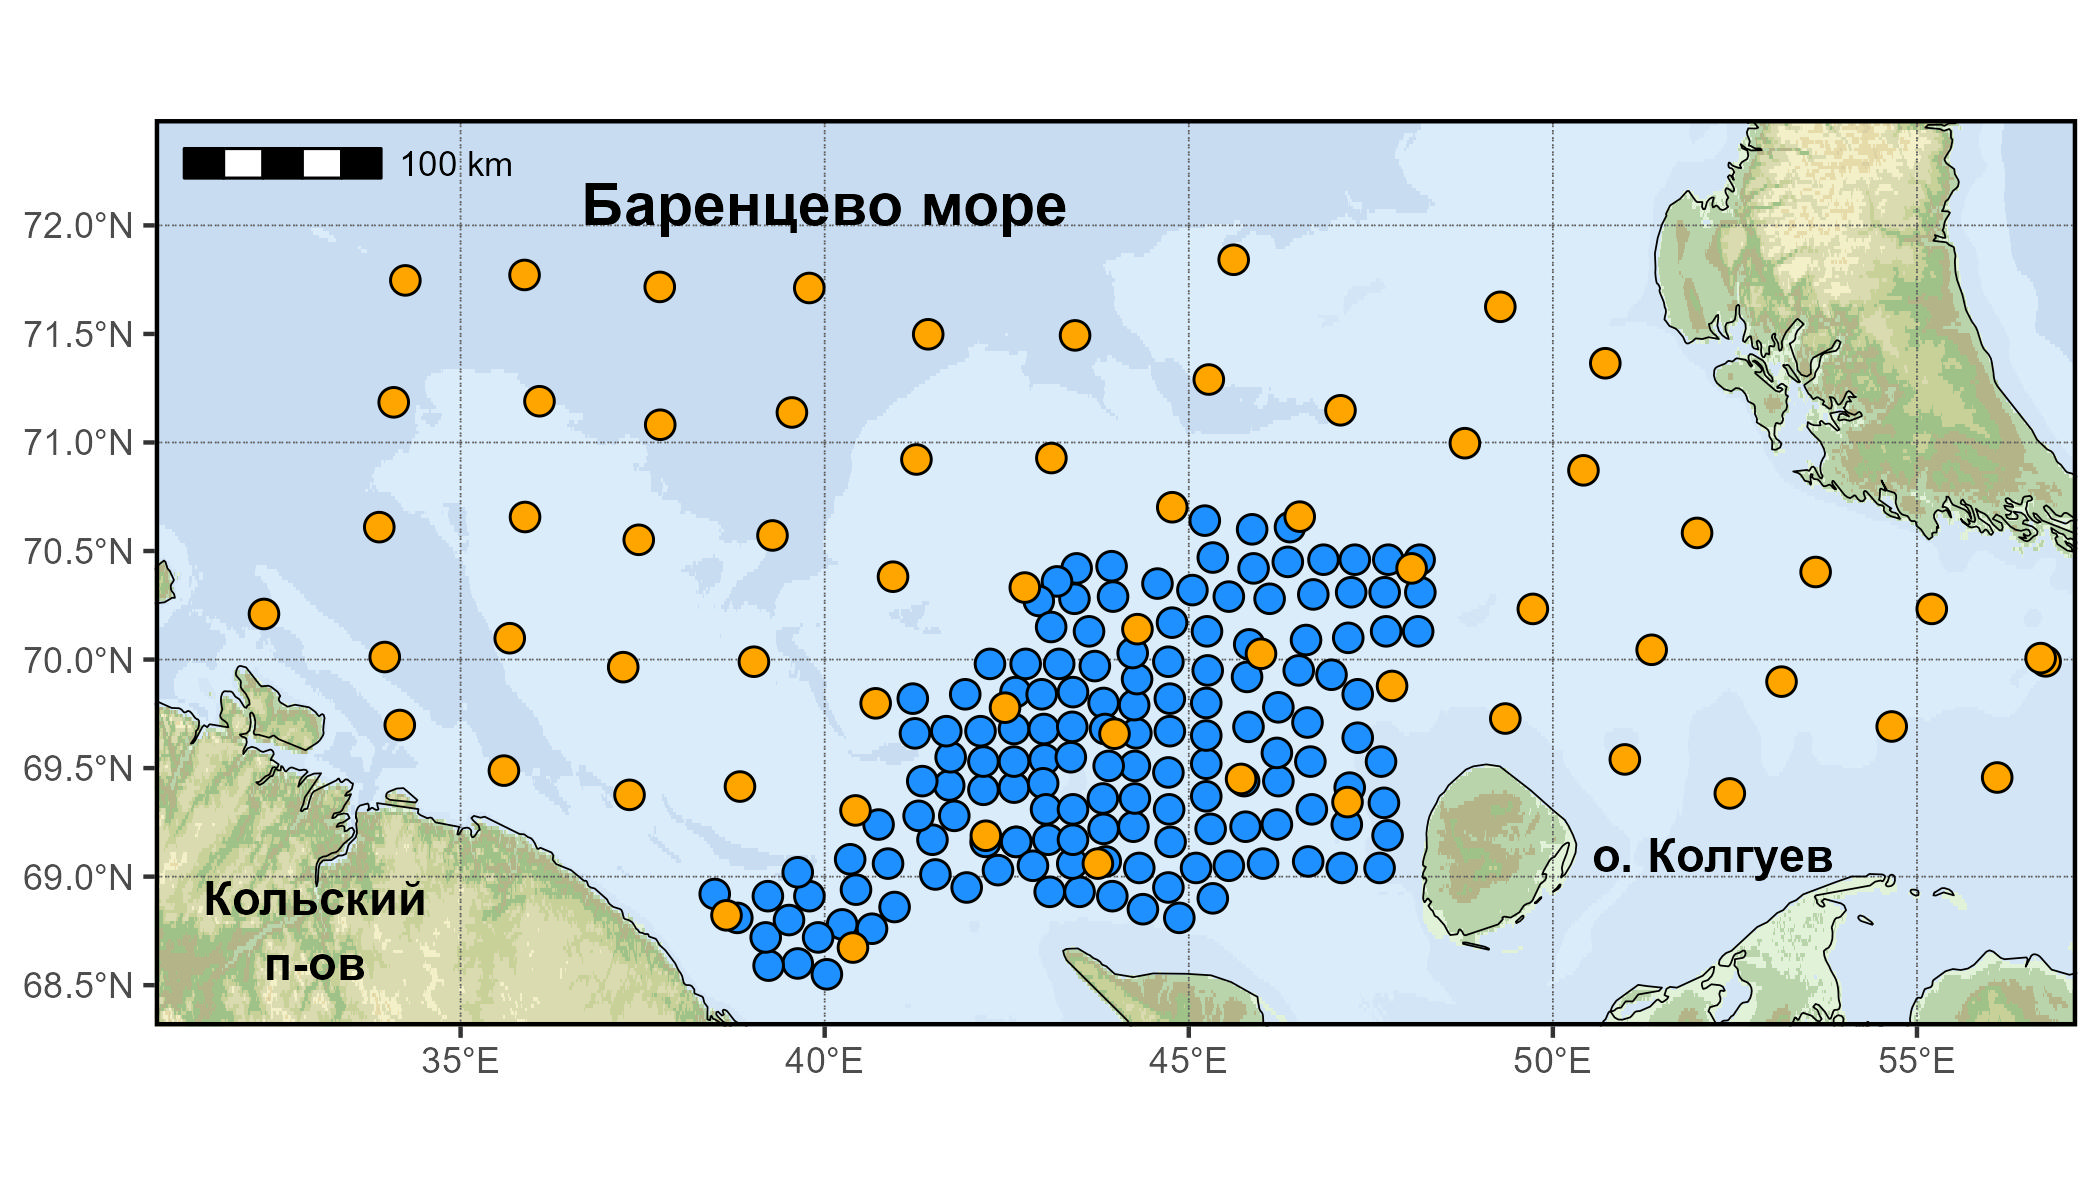
\includegraphics[width=0.8\linewidth,height=\textheight,keepaspectratio]{images/KARTOGRAPH13.jpg}

}

\caption{Рис. 13.: Карты для ``главы Материал и методы''}

\end{figure}%

\begin{Shaded}
\begin{Highlighting}[]
\CommentTok{\# Очистка окружения и установка рабочей директории}
\FunctionTok{rm}\NormalTok{(}\AttributeTok{list =} \FunctionTok{ls}\NormalTok{()) }\CommentTok{\# Удаление всех объектов из глобального окружения}
\FunctionTok{setwd}\NormalTok{(}\StringTok{"C:/COURSES/KARTOGRAPH/"}\NormalTok{) }\CommentTok{\# Установка рабочей директории}

\CommentTok{\# {-}{-}{-}{-}{-}{-}{-}{-}{-}{-}{-}{-}{-}{-}{-}{-}{-}}
\CommentTok{\# ЗАГРУЗКА ПАКЕТОВ}
\CommentTok{\# {-}{-}{-}{-}{-}{-}{-}{-}{-}{-}{-}{-}{-}{-}{-}{-}{-}}
\FunctionTok{library}\NormalTok{(sf)          }\CommentTok{\# Пространственные операции с векторными данными}
\FunctionTok{library}\NormalTok{(marmap)      }\CommentTok{\# Работа с батиметрическими данными (карты глубин)}
\FunctionTok{library}\NormalTok{(tidyverse)   }\CommentTok{\# Коллекция пакетов для обработки данных (dplyr, ggplot2 и др.)}
\FunctionTok{library}\NormalTok{(rnaturalearth) }\CommentTok{\# Векторные картографические данные (границы, береговые линии)}
\FunctionTok{library}\NormalTok{(ggspatial)   }\CommentTok{\# Инструменты для пространственной визуализации в ggplot}
\FunctionTok{library}\NormalTok{(readxl)      }\CommentTok{\# Импорт данных из Excel{-}файлов}

\CommentTok{\# {-}{-}{-}{-}{-}{-}{-}{-}{-}{-}{-}{-}{-}{-}{-}{-}{-}}
\CommentTok{\# ЗАГРУЗКА ДАННЫХ}
\CommentTok{\# {-}{-}{-}{-}{-}{-}{-}{-}{-}{-}{-}{-}{-}{-}{-}{-}{-}}
\CommentTok{\# Чтение данных из Excel{-}листа}
\NormalTok{DATA }\OtherTok{\textless{}{-}}\NormalTok{ readxl}\SpecialCharTok{::}\FunctionTok{read\_excel}\NormalTok{(}\StringTok{"KARTOGRAPHIC.xlsx"}\NormalTok{, }\AttributeTok{sheet =} \StringTok{"SURVEY"}\NormalTok{)}

\CommentTok{\# Фильтрация данных:}
\NormalTok{SUMMER }\OtherTok{\textless{}{-}}\NormalTok{ DATA[DATA}\SpecialCharTok{$}\NormalTok{SURV }\SpecialCharTok{==} \StringTok{"SUM"} \SpecialCharTok{\&}\NormalTok{ DATA}\SpecialCharTok{$}\NormalTok{YEAR }\SpecialCharTok{==} \DecValTok{2024}\NormalTok{, ] }\CommentTok{\# Летние исследования 2024}
\NormalTok{CRAB }\OtherTok{\textless{}{-}}\NormalTok{ DATA[DATA}\SpecialCharTok{$}\NormalTok{SURV }\SpecialCharTok{==} \StringTok{"CRAB"} \SpecialCharTok{\&}\NormalTok{ DATA}\SpecialCharTok{$}\NormalTok{YEAR }\SpecialCharTok{==} \DecValTok{2024}\NormalTok{, ]   }\CommentTok{\# Крабовые исследования 2024}

\CommentTok{\# {-}{-}{-}{-}{-}{-}{-}{-}{-}{-}{-}{-}{-}{-}{-}{-}{-}}
\CommentTok{\# ПОДГОТОВКА КАРТОГРАФИЧЕСКОЙ ОСНОВЫ}
\CommentTok{\# {-}{-}{-}{-}{-}{-}{-}{-}{-}{-}{-}{-}{-}{-}{-}{-}{-}}
\CommentTok{\# Загрузка векторных границ России}
\NormalTok{russia\_map }\OtherTok{\textless{}{-}} \FunctionTok{ne\_states}\NormalTok{(}\AttributeTok{country =} \StringTok{"russia"}\NormalTok{, }\AttributeTok{returnclass =} \StringTok{"sf"}\NormalTok{)}

\CommentTok{\# Загрузка береговой линии мирового океана}
\NormalTok{coast }\OtherTok{\textless{}{-}} \FunctionTok{ne\_coastline}\NormalTok{(}\AttributeTok{scale =} \DecValTok{10}\NormalTok{, }\AttributeTok{returnclass =} \StringTok{"sf"}\NormalTok{)}

\CommentTok{\# Создание сетки для навигации (5° по долготе, 1° по широте)}
\NormalTok{ga\_grid }\OtherTok{\textless{}{-}}\NormalTok{ russia\_map }\SpecialCharTok{\%\textgreater{}\%} 
  \FunctionTok{st\_make\_grid}\NormalTok{(}\AttributeTok{cellsize =} \FunctionTok{c}\NormalTok{(}\DecValTok{5}\NormalTok{, }\DecValTok{1}\NormalTok{), }\AttributeTok{offset =} \FunctionTok{c}\NormalTok{(}\DecValTok{30}\NormalTok{, }\DecValTok{67}\NormalTok{))}

\CommentTok{\# Установка границ региона интереса}
\NormalTok{xmin }\OtherTok{\textless{}{-}} \DecValTok{30}\NormalTok{; xmax }\OtherTok{\textless{}{-}} \DecValTok{58}
\NormalTok{ymin }\OtherTok{\textless{}{-}} \DecValTok{67}\NormalTok{; ymax }\OtherTok{\textless{}{-}} \FloatTok{72.5}

\CommentTok{\# {-}{-}{-}{-}{-}{-}{-}{-}{-}{-}{-}{-}{-}{-}{-}{-}{-}}
\CommentTok{\# БАТИМЕТРИЧЕСКИЕ ДАННЫЕ}
\CommentTok{\# {-}{-}{-}{-}{-}{-}{-}{-}{-}{-}{-}{-}{-}{-}{-}{-}{-}}
\CommentTok{\# Загрузка данных о глубинах из базы NOAA}
\NormalTok{bat }\OtherTok{\textless{}{-}} \FunctionTok{getNOAA.bathy}\NormalTok{(}
  \AttributeTok{lon1 =}\NormalTok{ xmin, }\AttributeTok{lon2 =}\NormalTok{ xmax,}
  \AttributeTok{lat1 =}\NormalTok{ ymin, }\AttributeTok{lat2 =}\NormalTok{ ymax,}
  \AttributeTok{resolution =} \DecValTok{1}\NormalTok{,   }\CommentTok{\# Разрешение данных (1 минута дуги)}
  \AttributeTok{keep =} \ConstantTok{TRUE}       \CommentTok{\# Сохранить кэш на диске}
\NormalTok{)}

\CommentTok{\# Преобразование в таблицу XYZ (долгота, широта, глубина)}
\NormalTok{bat\_xyz }\OtherTok{\textless{}{-}} \FunctionTok{as.xyz}\NormalTok{(bat)}

\CommentTok{\# Создание цветовой схемы для глубин:}
\NormalTok{breaks }\OtherTok{\textless{}{-}} \FunctionTok{c}\NormalTok{(}\SpecialCharTok{{-}}\DecValTok{10000}\NormalTok{, }\SpecialCharTok{{-}}\DecValTok{7000}\NormalTok{, }\SpecialCharTok{{-}}\DecValTok{6000}\NormalTok{, }\SpecialCharTok{{-}}\DecValTok{5000}\NormalTok{, }\SpecialCharTok{{-}}\DecValTok{4000}\NormalTok{, }\SpecialCharTok{{-}}\DecValTok{3000}\NormalTok{, }\SpecialCharTok{{-}}\DecValTok{2000}\NormalTok{, }\SpecialCharTok{{-}}\DecValTok{1000}\NormalTok{, }
            \SpecialCharTok{{-}}\DecValTok{500}\NormalTok{, }\SpecialCharTok{{-}}\DecValTok{200}\NormalTok{, }\SpecialCharTok{{-}}\DecValTok{50}\NormalTok{, }\SpecialCharTok{{-}}\DecValTok{1}\NormalTok{, }\DecValTok{5}\NormalTok{, }\DecValTok{50}\NormalTok{, }\DecValTok{100}\NormalTok{, }\DecValTok{150}\NormalTok{, }\DecValTok{200}\NormalTok{, }\DecValTok{300}\NormalTok{, }\DecValTok{400}\NormalTok{, }\DecValTok{500}\NormalTok{, }\DecValTok{1000}\NormalTok{, }\DecValTok{3000}\NormalTok{)}
\NormalTok{cols }\OtherTok{\textless{}{-}} \FunctionTok{c}\NormalTok{(}
  \StringTok{"\#5e99d6"}\NormalTok{, }\StringTok{"\#669cd4"}\NormalTok{, }\StringTok{"\#6c9fd4"}\NormalTok{, }\StringTok{"\#96bce3"}\NormalTok{, }\StringTok{"\#AEC8E3"}\NormalTok{, }\StringTok{"\#a6c4e3"}\NormalTok{,}
  \StringTok{"\#AEC8E3"}\NormalTok{, }\StringTok{"\#BBD0EB"}\NormalTok{, }\StringTok{"\#C7DCF1"}\NormalTok{, }\StringTok{"\#DAECFA"}\NormalTok{, }\StringTok{"\#D2E5F6"}\NormalTok{, }\StringTok{"\#e1f2d8"}\NormalTok{,}
  \StringTok{"\#B8D3AA"}\NormalTok{, }\StringTok{"\#b3b387"}\NormalTok{, }\StringTok{"\#9EC187"}\NormalTok{, }\StringTok{"\#C7D097"}\NormalTok{, }\StringTok{"\#DADBAF"}\NormalTok{, }\StringTok{"\#F3F0C7"}\NormalTok{,}
  \StringTok{"\#E6DBA8"}\NormalTok{, }\StringTok{"\#DACFA1"}\NormalTok{, }\StringTok{"\#D1BF81"}\NormalTok{, }\StringTok{"\#C69D45"}
\NormalTok{)}

\CommentTok{\# Категоризация глубин для визуализации}
\NormalTok{bat\_xyz}\SpecialCharTok{$}\NormalTok{V4 }\OtherTok{\textless{}{-}} \FunctionTok{cut}\NormalTok{(bat\_xyz}\SpecialCharTok{$}\NormalTok{V3, }\AttributeTok{breaks =}\NormalTok{ breaks)}
\NormalTok{niveles }\OtherTok{\textless{}{-}} \FunctionTok{levels}\NormalTok{(bat\_xyz}\SpecialCharTok{$}\NormalTok{V4)  }\CommentTok{\# Сохранение уровней для легенды}

\CommentTok{\# {-}{-}{-}{-}{-}{-}{-}{-}{-}{-}{-}{-}{-}{-}{-}{-}{-}}
\CommentTok{\# ПОСТРОЕНИЕ БАЗОВОЙ КАРТЫ}
\CommentTok{\# {-}{-}{-}{-}{-}{-}{-}{-}{-}{-}{-}{-}{-}{-}{-}{-}{-}}
\NormalTok{map }\OtherTok{\textless{}{-}} \FunctionTok{ggplot}\NormalTok{() }\SpecialCharTok{+}
  \CommentTok{\# Векторные границы России}
  \FunctionTok{geom\_sf}\NormalTok{(}\AttributeTok{data =}\NormalTok{ russia\_map) }\SpecialCharTok{+}
  \CommentTok{\# Батиметрическая подложка (цвет = глубина)}
  \FunctionTok{geom\_tile}\NormalTok{(}\AttributeTok{data =}\NormalTok{ bat\_xyz, }\FunctionTok{aes}\NormalTok{(}\AttributeTok{x =}\NormalTok{ V1, }\AttributeTok{y =}\NormalTok{ V2, }\AttributeTok{fill =}\NormalTok{ V4), }\AttributeTok{show.legend =} \ConstantTok{FALSE}\NormalTok{) }\SpecialCharTok{+}
  \CommentTok{\# Цветовая схема для глубин}
  \FunctionTok{scale\_fill\_manual}\NormalTok{(}\AttributeTok{name =} \StringTok{"Глубина"}\NormalTok{, }\AttributeTok{values =}\NormalTok{ cols, }\AttributeTok{breaks =}\NormalTok{ niveles) }\SpecialCharTok{+}
  \CommentTok{\# Наложение сетки}
  \FunctionTok{geom\_sf}\NormalTok{(}\AttributeTok{data =}\NormalTok{ ga\_grid, }\AttributeTok{alpha =} \FloatTok{0.01}\NormalTok{, }\AttributeTok{linetype =} \DecValTok{3}\NormalTok{) }\SpecialCharTok{+}
  \CommentTok{\# Береговая линия}
  \FunctionTok{geom\_sf}\NormalTok{(}\AttributeTok{data =}\NormalTok{ coast, }\AttributeTok{linewidth =} \FloatTok{0.2}\NormalTok{, }\AttributeTok{fill =} \ConstantTok{NA}\NormalTok{) }\SpecialCharTok{+}
  \CommentTok{\# Ограничение области карты}
  \FunctionTok{coord\_sf}\NormalTok{(}\AttributeTok{xlim =} \FunctionTok{c}\NormalTok{(}\DecValTok{32}\NormalTok{, }\DecValTok{56}\NormalTok{), }\AttributeTok{ylim =} \FunctionTok{c}\NormalTok{(}\FloatTok{68.5}\NormalTok{, }\FloatTok{72.3}\NormalTok{)) }\SpecialCharTok{+}
  \CommentTok{\# Масштабная линейка (top{-}left)}
  \FunctionTok{annotation\_scale}\NormalTok{(}\AttributeTok{location =} \StringTok{"tl"}\NormalTok{, }\AttributeTok{width\_hint =} \FloatTok{0.2}\NormalTok{) }\SpecialCharTok{+}
  \CommentTok{\# Оформление}
  \FunctionTok{labs}\NormalTok{(}\AttributeTok{x =} \ConstantTok{NULL}\NormalTok{, }\AttributeTok{y =} \ConstantTok{NULL}\NormalTok{, }\AttributeTok{fill =} \StringTok{"Глубина (м)"}\NormalTok{) }\SpecialCharTok{+}
  \FunctionTok{theme}\NormalTok{(}\AttributeTok{panel.border =} \FunctionTok{element\_rect}\NormalTok{(}\AttributeTok{colour =} \StringTok{"black"}\NormalTok{, }\AttributeTok{fill =} \ConstantTok{NA}\NormalTok{, }\AttributeTok{linewidth =} \DecValTok{1}\NormalTok{))}

\CommentTok{\# {-}{-}{-}{-}{-}{-}{-}{-}{-}{-}{-}{-}{-}{-}{-}{-}{-}}
\CommentTok{\# ДОБАВЛЕНИЕ АННОТАЦИЙ}
\CommentTok{\# {-}{-}{-}{-}{-}{-}{-}{-}{-}{-}{-}{-}{-}{-}{-}{-}{-}}
\NormalTok{map }\OtherTok{\textless{}{-}}\NormalTok{ map }\SpecialCharTok{+}
  \FunctionTok{annotate}\NormalTok{(}\StringTok{"text"}\NormalTok{, }\AttributeTok{x =} \DecValTok{40}\NormalTok{, }\AttributeTok{y =} \FloatTok{72.1}\NormalTok{, }\AttributeTok{size =} \DecValTok{5}\NormalTok{, }
           \AttributeTok{label =} \StringTok{"Баренцево море"}\NormalTok{, }\AttributeTok{fontface =} \StringTok{"bold"}\NormalTok{) }\SpecialCharTok{+}
  \FunctionTok{annotate}\NormalTok{(}\StringTok{"text"}\NormalTok{, }\AttributeTok{x =} \FloatTok{52.2}\NormalTok{, }\AttributeTok{y =} \FloatTok{69.1}\NormalTok{, }\AttributeTok{size =} \DecValTok{4}\NormalTok{, }
           \AttributeTok{label =} \StringTok{"о. Колгуев"}\NormalTok{, }\AttributeTok{fontface =} \StringTok{"bold"}\NormalTok{) }\SpecialCharTok{+}
  \FunctionTok{annotate}\NormalTok{(}\StringTok{"text"}\NormalTok{, }\AttributeTok{x =} \DecValTok{33}\NormalTok{, }\AttributeTok{y =} \FloatTok{68.9}\NormalTok{, }\AttributeTok{size =} \DecValTok{4}\NormalTok{, }
           \AttributeTok{label =} \StringTok{"Кольский"}\NormalTok{, }\AttributeTok{fontface =} \StringTok{"bold"}\NormalTok{) }\SpecialCharTok{+}
  \FunctionTok{annotate}\NormalTok{(}\StringTok{"text"}\NormalTok{, }\AttributeTok{x =} \DecValTok{33}\NormalTok{, }\AttributeTok{y =} \FloatTok{68.6}\NormalTok{, }\AttributeTok{size =} \DecValTok{4}\NormalTok{, }
           \AttributeTok{label =} \StringTok{"п{-}ов"}\NormalTok{, }\AttributeTok{fontface =} \StringTok{"bold"}\NormalTok{)}

\CommentTok{\# {-}{-}{-}{-}{-}{-}{-}{-}{-}{-}{-}{-}{-}{-}{-}{-}{-}}
\CommentTok{\# ДОБАВЛЕНИЕ ТОЧЕК НАБЛЮДЕНИЙ}
\CommentTok{\# {-}{-}{-}{-}{-}{-}{-}{-}{-}{-}{-}{-}{-}{-}{-}{-}{-}}
\NormalTok{map }\OtherTok{\textless{}{-}}\NormalTok{ map }\SpecialCharTok{+}
  \CommentTok{\# Точки исследований краба (синие)}
  \FunctionTok{geom\_point}\NormalTok{(}
    \AttributeTok{data =}\NormalTok{ CRAB, }
    \FunctionTok{aes}\NormalTok{(}\AttributeTok{x =}\NormalTok{ X }\SpecialCharTok{+} \FloatTok{0.2}\NormalTok{, }\AttributeTok{y =}\NormalTok{ Y), }\CommentTok{\# Смещение для визуального разделения}
    \AttributeTok{size =} \DecValTok{3}\NormalTok{, }\AttributeTok{color =} \StringTok{"black"}\NormalTok{, }\AttributeTok{fill =} \StringTok{"\#1E90FF"}\NormalTok{, }
    \AttributeTok{shape =} \DecValTok{21}\NormalTok{, }\AttributeTok{alpha =} \DecValTok{1}
\NormalTok{  ) }\SpecialCharTok{+}
  \CommentTok{\# Точки летних исследований (оранжевые)}
  \FunctionTok{geom\_point}\NormalTok{(}
    \AttributeTok{data =}\NormalTok{ SUMMER, }
    \FunctionTok{aes}\NormalTok{(}\AttributeTok{x =}\NormalTok{ X, }\AttributeTok{y =}\NormalTok{ Y), }
    \AttributeTok{size =} \DecValTok{3}\NormalTok{, }\AttributeTok{color =} \StringTok{"black"}\NormalTok{, }\AttributeTok{fill =} \StringTok{"\#FFA500"}\NormalTok{, }
    \AttributeTok{shape =} \DecValTok{21}\NormalTok{, }\AttributeTok{alpha =} \DecValTok{1}
\NormalTok{  )}

\CommentTok{\# Вывод финальной карты}
\FunctionTok{print}\NormalTok{(map)}

\CommentTok{\# {-}{-}{-}{-}{-}{-}{-}{-}{-}{-}{-}{-}{-}{-}{-}{-}{-}}
\CommentTok{\# СОХРАНЕНИЕ РЕЗУЛЬТАТА}
\CommentTok{\# {-}{-}{-}{-}{-}{-}{-}{-}{-}{-}{-}{-}{-}{-}{-}{-}{-}}
\FunctionTok{ggsave}\NormalTok{(}\StringTok{"DATA\_MAP.jpg"}\NormalTok{, }
       \AttributeTok{plot =}\NormalTok{ map,          }\CommentTok{\# Используем явное указание объекта}
       \AttributeTok{device =} \StringTok{"jpeg"}\NormalTok{, }
       \AttributeTok{dpi =} \DecValTok{600}\NormalTok{,           }\CommentTok{\# Высокое разрешение}
       \AttributeTok{width =} \DecValTok{7}\NormalTok{,           }\CommentTok{\# Ширина в дюймах}
       \AttributeTok{height =} \DecValTok{5}\NormalTok{,          }\CommentTok{\# Высота в дюймах}
       \AttributeTok{units =} \StringTok{"in"}\NormalTok{)}
\end{Highlighting}
\end{Shaded}

\section{Карты с картой-врезкой и
маршрутом}\label{ux43aux430ux440ux442ux44b-ux441-ux43aux430ux440ux442ux43eux439-ux432ux440ux435ux437ux43aux43eux439-ux438-ux43cux430ux440ux448ux440ux443ux442ux43eux43c}

\begin{figure}[H]

{\centering 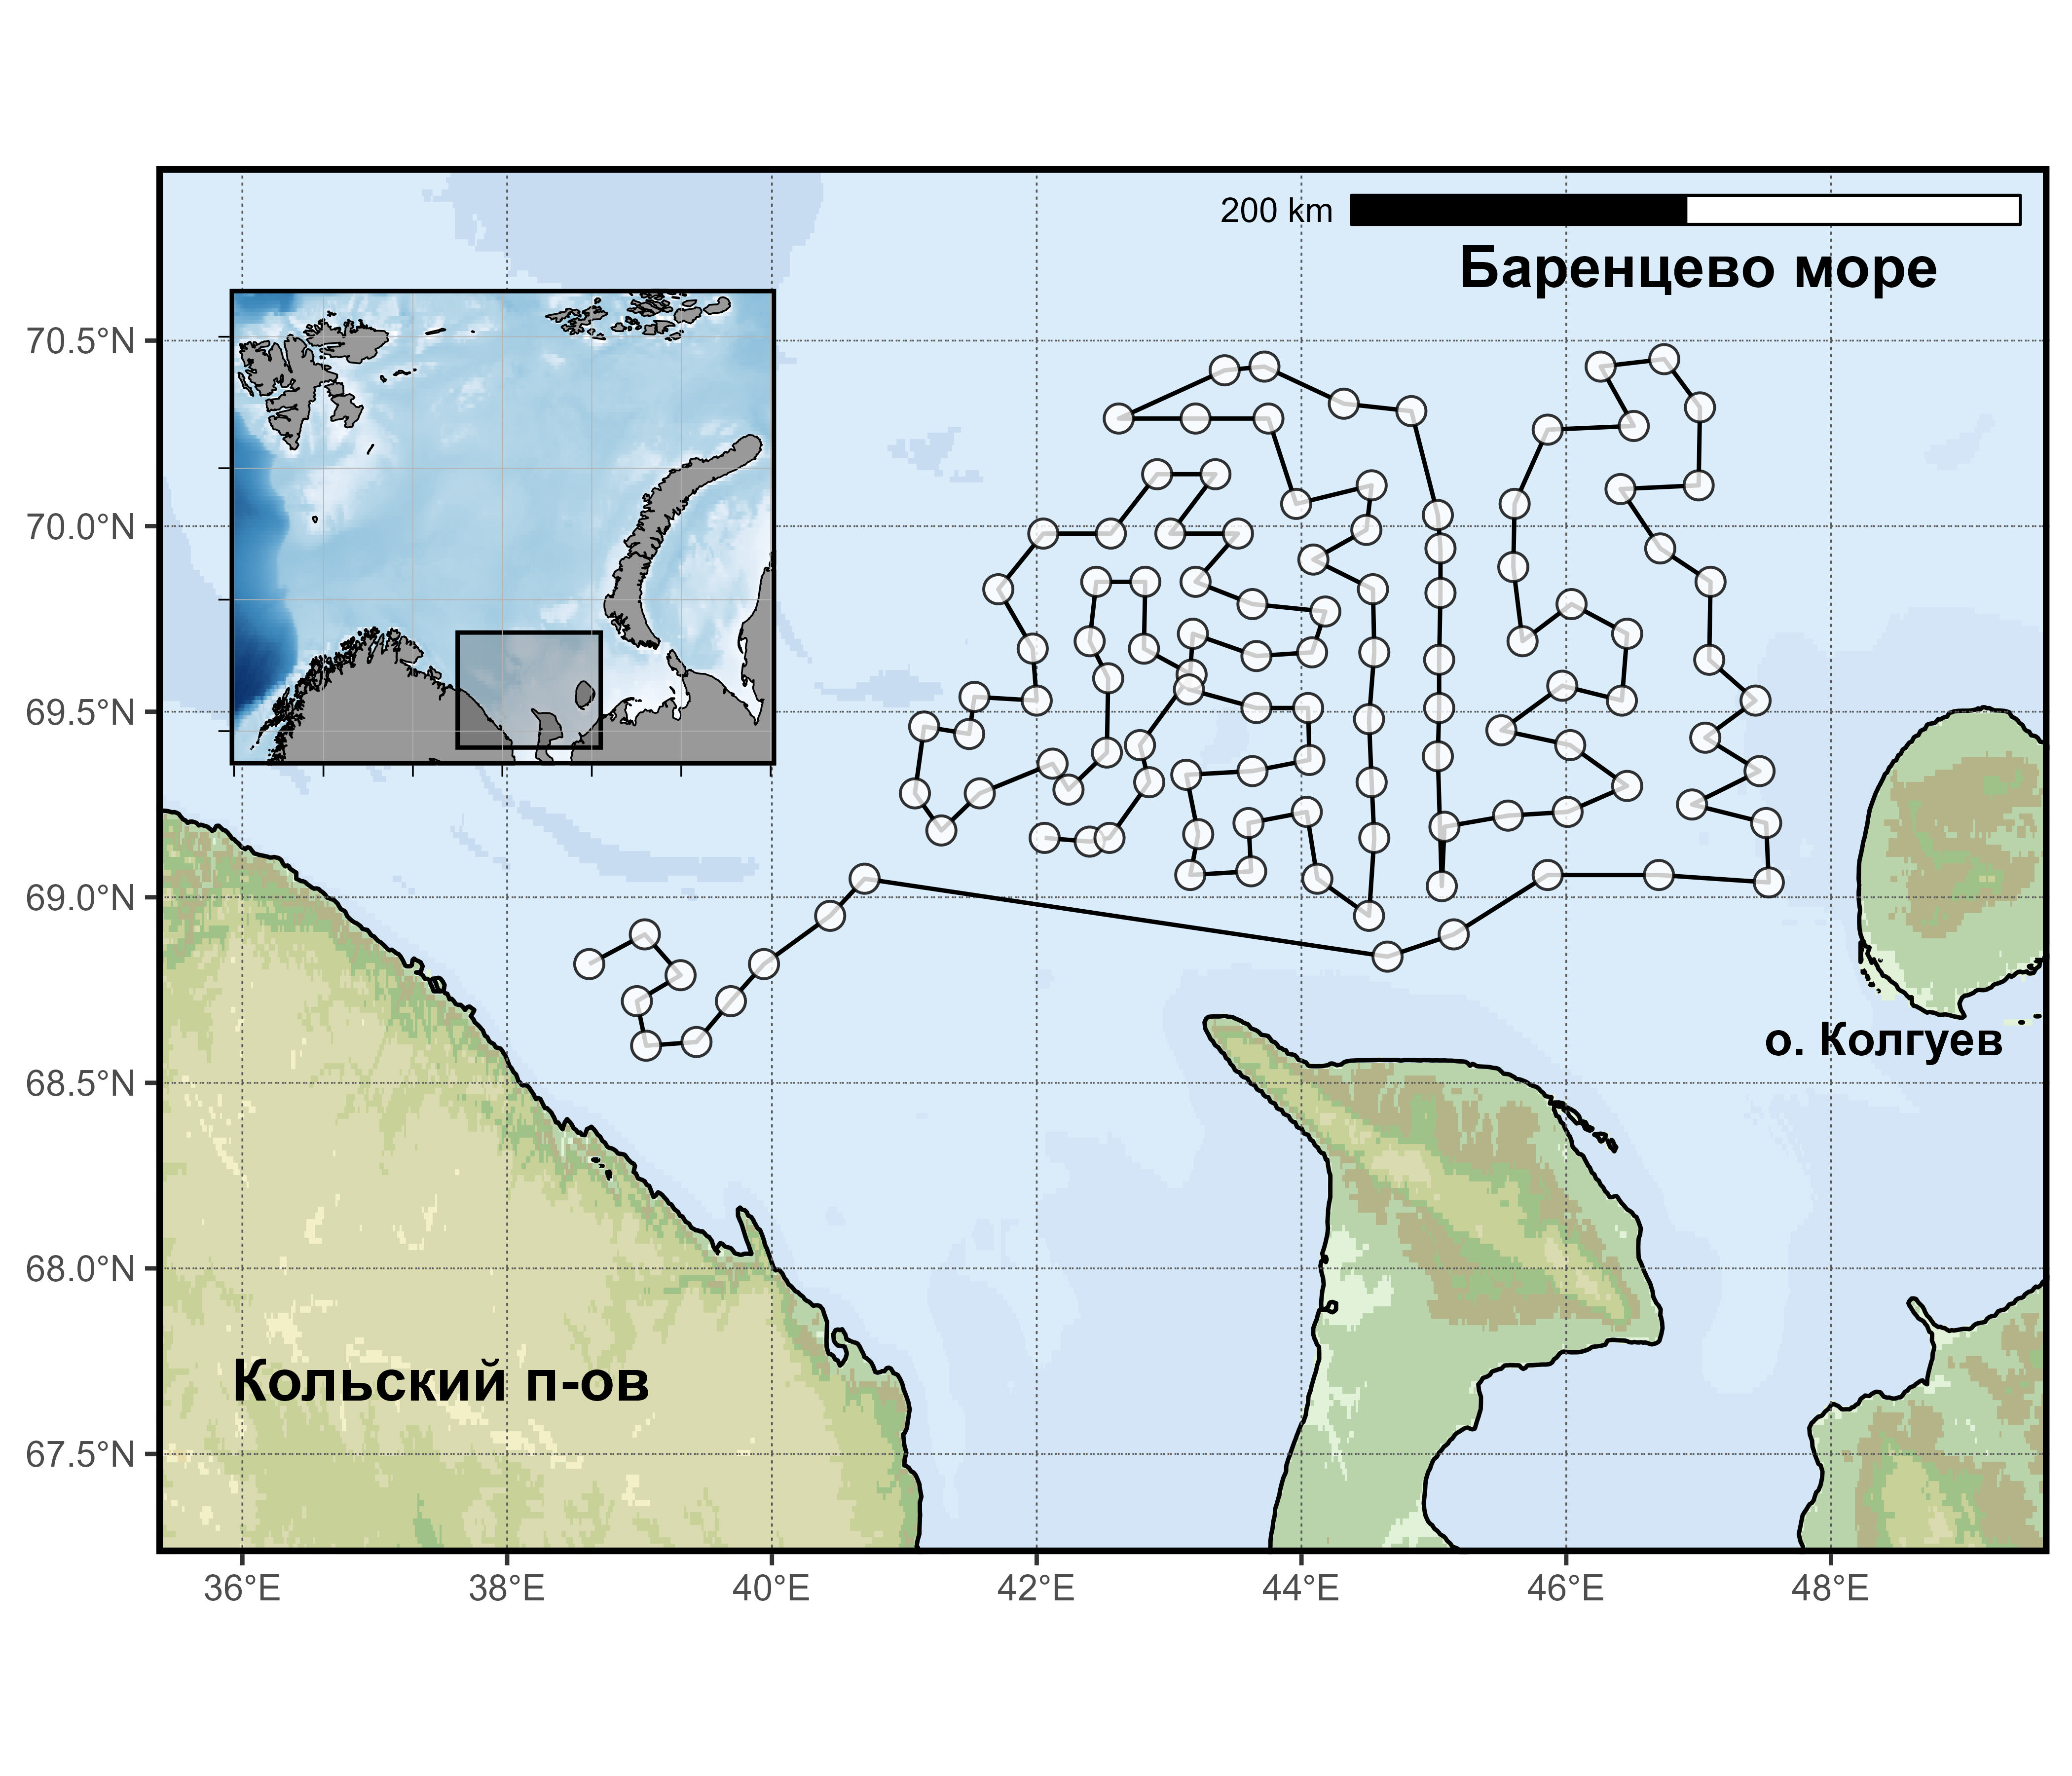
\includegraphics[width=0.8\linewidth,height=\textheight,keepaspectratio]{images/KARTOGRAPH14.jpg}

}

\caption{Рис. 14.: Карты с картой-врезкой и маршрутом}

\end{figure}%

\begin{Shaded}
\begin{Highlighting}[]
\CommentTok{\# Очистка окружения и установка рабочей директории}
\FunctionTok{rm}\NormalTok{(}\AttributeTok{list =} \FunctionTok{ls}\NormalTok{()) }\CommentTok{\# Удаление всех объектов из глобального окружения}
\FunctionTok{setwd}\NormalTok{(}\StringTok{"C:/COURSES/KARTOGRAPH/"}\NormalTok{) }\CommentTok{\# Установка рабочей директории}

\CommentTok{\# {-}{-}{-}{-}{-}{-}{-}{-}{-}{-}{-}{-}{-}{-}{-}{-}{-}}
\CommentTok{\# ЗАГРУЗКА ПАКЕТОВ}
\CommentTok{\# {-}{-}{-}{-}{-}{-}{-}{-}{-}{-}{-}{-}{-}{-}{-}{-}{-}}
\FunctionTok{library}\NormalTok{(sf)          }\CommentTok{\# Пространственные операции с векторными данными}
\FunctionTok{library}\NormalTok{(marmap)      }\CommentTok{\# Работа с батиметрическими данными (карты глубин)}
\FunctionTok{library}\NormalTok{(tidyverse)   }\CommentTok{\# Коллекция пакетов для обработки данных}
\FunctionTok{library}\NormalTok{(rnaturalearth) }\CommentTok{\# Векторные картографические данные}
\FunctionTok{library}\NormalTok{(ggspatial)   }\CommentTok{\# Инструменты для пространственной визуализации}
\FunctionTok{library}\NormalTok{(readxl)      }\CommentTok{\# Импорт данных из Excel}
\FunctionTok{library}\NormalTok{(ggOceanMaps) }\CommentTok{\# Специализированные карты океанов}
\FunctionTok{library}\NormalTok{(cowplot)     }\CommentTok{\# Компоновка графиков и добавление элементов}

\CommentTok{\# {-}{-}{-}{-}{-}{-}{-}{-}{-}{-}{-}{-}{-}{-}{-}{-}{-}}
\CommentTok{\# ЗАГРУЗКА ДАННЫХ}
\CommentTok{\# {-}{-}{-}{-}{-}{-}{-}{-}{-}{-}{-}{-}{-}{-}{-}{-}{-}}
\CommentTok{\# Чтение данных из Excel}
\NormalTok{DATA }\OtherTok{\textless{}{-}}\NormalTok{ readxl}\SpecialCharTok{::}\FunctionTok{read\_excel}\NormalTok{(}\StringTok{"KARTOGRAPHIC.xlsx"}\NormalTok{, }\AttributeTok{sheet =} \StringTok{"SURVEY"}\NormalTok{)}

\CommentTok{\# Фильтрация данных (крабовые исследования 2022)}
\NormalTok{DATA }\OtherTok{\textless{}{-}}\NormalTok{ DATA[DATA}\SpecialCharTok{$}\NormalTok{SURV }\SpecialCharTok{==} \StringTok{"CRAB"} \SpecialCharTok{\&}\NormalTok{ DATA}\SpecialCharTok{$}\NormalTok{YEAR }\SpecialCharTok{==} \DecValTok{2022}\NormalTok{, ]}

\CommentTok{\# Загрузка векторных границ России}
\NormalTok{russia\_map }\OtherTok{\textless{}{-}} \FunctionTok{ne\_states}\NormalTok{(}\AttributeTok{country =} \StringTok{"russia"}\NormalTok{, }\AttributeTok{returnclass =} \StringTok{"sf"}\NormalTok{)}

\CommentTok{\# Установка границ региона интереса}
\NormalTok{xmin }\OtherTok{\textless{}{-}} \DecValTok{35}\NormalTok{; xmax }\OtherTok{\textless{}{-}} \DecValTok{50}
\NormalTok{ymin }\OtherTok{\textless{}{-}} \FloatTok{67.2}\NormalTok{; ymax }\OtherTok{\textless{}{-}} \DecValTok{71}

\CommentTok{\# {-}{-}{-}{-}{-}{-}{-}{-}{-}{-}{-}{-}{-}{-}{-}{-}{-}}
\CommentTok{\# БАТИМЕТРИЧЕСКИЕ ДАННЫЕ}
\CommentTok{\# {-}{-}{-}{-}{-}{-}{-}{-}{-}{-}{-}{-}{-}{-}{-}{-}{-}}
\CommentTok{\# Загрузка данных о глубинах}
\NormalTok{bat }\OtherTok{\textless{}{-}} \FunctionTok{getNOAA.bathy}\NormalTok{(xmin, xmax, ymin, ymax, }\AttributeTok{resolution =} \DecValTok{1}\NormalTok{, }\AttributeTok{keep =} \ConstantTok{TRUE}\NormalTok{)}
\NormalTok{bat\_xyz }\OtherTok{\textless{}{-}} \FunctionTok{as.xyz}\NormalTok{(bat)}

\CommentTok{\# Определение цветовых уровней для глубин}
\NormalTok{breaks }\OtherTok{\textless{}{-}} \FunctionTok{c}\NormalTok{(}\SpecialCharTok{{-}}\DecValTok{10000}\NormalTok{, }\SpecialCharTok{{-}}\DecValTok{7000}\NormalTok{, }\SpecialCharTok{{-}}\DecValTok{6000}\NormalTok{, }\SpecialCharTok{{-}}\DecValTok{5000}\NormalTok{, }\SpecialCharTok{{-}}\DecValTok{4000}\NormalTok{, }\SpecialCharTok{{-}}\DecValTok{3000}\NormalTok{, }\SpecialCharTok{{-}}\DecValTok{2000}\NormalTok{, }\SpecialCharTok{{-}}\DecValTok{1000}\NormalTok{, }
            \SpecialCharTok{{-}}\DecValTok{500}\NormalTok{, }\SpecialCharTok{{-}}\DecValTok{200}\NormalTok{, }\SpecialCharTok{{-}}\DecValTok{50}\NormalTok{, }\SpecialCharTok{{-}}\DecValTok{1}\NormalTok{, }\DecValTok{5}\NormalTok{, }\DecValTok{50}\NormalTok{, }\DecValTok{100}\NormalTok{, }\DecValTok{150}\NormalTok{, }\DecValTok{200}\NormalTok{, }\DecValTok{300}\NormalTok{, }\DecValTok{400}\NormalTok{, }\DecValTok{500}\NormalTok{, }\DecValTok{1000}\NormalTok{, }\DecValTok{3000}\NormalTok{)}
\NormalTok{cols }\OtherTok{\textless{}{-}} \FunctionTok{c}\NormalTok{(}
  \StringTok{"\#5e99d6"}\NormalTok{, }\StringTok{"\#669cd4"}\NormalTok{, }\StringTok{"\#6c9fd4"}\NormalTok{, }\StringTok{"\#96bce3"}\NormalTok{, }\StringTok{"\#AEC8E3"}\NormalTok{, }\StringTok{"\#a6c4e3"}\NormalTok{,}
  \StringTok{"\#AEC8E3"}\NormalTok{, }\StringTok{"\#BBD0EB"}\NormalTok{, }\StringTok{"\#C7DCF1"}\NormalTok{, }\StringTok{"\#DAECFA"}\NormalTok{, }\StringTok{"\#D2E5F6"}\NormalTok{, }\StringTok{"\#e1f2d8"}\NormalTok{,}
  \StringTok{"\#B8D3AA"}\NormalTok{, }\StringTok{"\#b3b387"}\NormalTok{, }\StringTok{"\#9EC187"}\NormalTok{, }\StringTok{"\#C7D097"}\NormalTok{, }\StringTok{"\#DADBAF"}\NormalTok{, }\StringTok{"\#F3F0C7"}\NormalTok{,}
  \StringTok{"\#E6DBA8"}\NormalTok{, }\StringTok{"\#DACFA1"}\NormalTok{, }\StringTok{"\#D1BF81"}\NormalTok{, }\StringTok{"\#C69D45"}
\NormalTok{)}

\CommentTok{\# Категоризация глубин}
\NormalTok{bat\_xyz}\SpecialCharTok{$}\NormalTok{V4 }\OtherTok{\textless{}{-}} \FunctionTok{cut}\NormalTok{(bat\_xyz}\SpecialCharTok{$}\NormalTok{V3, }\AttributeTok{breaks =}\NormalTok{ breaks)}
\NormalTok{niveles }\OtherTok{\textless{}{-}} \FunctionTok{levels}\NormalTok{(bat\_xyz}\SpecialCharTok{$}\NormalTok{V4)}

\CommentTok{\# Создание координатной сетки}
\NormalTok{ga\_grid }\OtherTok{\textless{}{-}}\NormalTok{ russia\_map }\SpecialCharTok{\%\textgreater{}\%} 
  \FunctionTok{st\_make\_grid}\NormalTok{(}\AttributeTok{cellsize =} \FunctionTok{c}\NormalTok{(}\DecValTok{2}\NormalTok{, }\FloatTok{0.5}\NormalTok{), }\AttributeTok{offset =} \FunctionTok{c}\NormalTok{(}\DecValTok{34}\NormalTok{, }\DecValTok{67}\NormalTok{))}

\CommentTok{\# {-}{-}{-}{-}{-}{-}{-}{-}{-}{-}{-}{-}{-}{-}{-}{-}{-}}
\CommentTok{\# ПОСТРОЕНИЕ ОСНОВНОЙ КАРТЫ}
\CommentTok{\# {-}{-}{-}{-}{-}{-}{-}{-}{-}{-}{-}{-}{-}{-}{-}{-}{-}}
\NormalTok{map }\OtherTok{\textless{}{-}} \FunctionTok{ggplot}\NormalTok{() }\SpecialCharTok{+}
  \CommentTok{\# Векторные границы России}
  \FunctionTok{geom\_sf}\NormalTok{(}\AttributeTok{data =}\NormalTok{ russia\_map) }\SpecialCharTok{+}
  \CommentTok{\# Батиметрическая подложка}
  \FunctionTok{geom\_tile}\NormalTok{(}\AttributeTok{data =}\NormalTok{ bat\_xyz, }\FunctionTok{aes}\NormalTok{(}\AttributeTok{x =}\NormalTok{ V1, }\AttributeTok{y =}\NormalTok{ V2, }\AttributeTok{fill =}\NormalTok{ V4), }\AttributeTok{show.legend =} \ConstantTok{FALSE}\NormalTok{) }\SpecialCharTok{+}
  \FunctionTok{scale\_fill\_manual}\NormalTok{(}\AttributeTok{values =}\NormalTok{ cols, }\AttributeTok{breaks =}\NormalTok{ niveles) }\SpecialCharTok{+}
  \CommentTok{\# Контур нулевой глубины (береговая линия)}
  \FunctionTok{geom\_contour}\NormalTok{(}\AttributeTok{data =}\NormalTok{ bat\_xyz, }\FunctionTok{aes}\NormalTok{(}\AttributeTok{x =}\NormalTok{ V1, }\AttributeTok{y =}\NormalTok{ V2, }\AttributeTok{z =}\NormalTok{ V3), }
               \AttributeTok{breaks =} \DecValTok{0}\NormalTok{, }\AttributeTok{color =} \StringTok{"black"}\NormalTok{, }\AttributeTok{linewidth =} \FloatTok{0.5}\NormalTok{) }\SpecialCharTok{+} 
  \CommentTok{\# Координатная сетка}
  \FunctionTok{geom\_sf}\NormalTok{(}\AttributeTok{data =}\NormalTok{ ga\_grid, }\AttributeTok{alpha =} \FloatTok{0.01}\NormalTok{, }\AttributeTok{linetype =} \DecValTok{3}\NormalTok{) }\SpecialCharTok{+}
  \CommentTok{\# Ограничение области карты}
  \FunctionTok{coord\_sf}\NormalTok{(}\AttributeTok{xlim =} \FunctionTok{c}\NormalTok{(}\DecValTok{36}\NormalTok{, }\DecValTok{49}\NormalTok{), }\AttributeTok{ylim =} \FunctionTok{c}\NormalTok{(}\FloatTok{67.4}\NormalTok{, }\FloatTok{70.8}\NormalTok{)) }\SpecialCharTok{+} 
  \CommentTok{\# Масштабная линейка}
  \FunctionTok{annotation\_scale}\NormalTok{(}\AttributeTok{location =} \StringTok{"tr"}\NormalTok{, }\AttributeTok{width\_hint =} \FloatTok{0.5}\NormalTok{) }\SpecialCharTok{+}
  \FunctionTok{labs}\NormalTok{(}\AttributeTok{x =} \ConstantTok{NULL}\NormalTok{, }\AttributeTok{y =} \ConstantTok{NULL}\NormalTok{) }\SpecialCharTok{+}
  \CommentTok{\# Географические подписи}
  \FunctionTok{annotate}\NormalTok{(}\StringTok{"text"}\NormalTok{, }\AttributeTok{x =} \DecValTok{47}\NormalTok{, }\AttributeTok{y =} \FloatTok{70.7}\NormalTok{, }\AttributeTok{size =} \DecValTok{5}\NormalTok{, }
           \AttributeTok{label =} \StringTok{"Баренцево море"}\NormalTok{, }\AttributeTok{fontface =} \StringTok{"bold"}\NormalTok{) }\SpecialCharTok{+}
  \FunctionTok{annotate}\NormalTok{(}\StringTok{"text"}\NormalTok{, }\AttributeTok{x =} \FloatTok{48.4}\NormalTok{, }\AttributeTok{y =} \FloatTok{68.62}\NormalTok{, }\AttributeTok{size =} \DecValTok{4}\NormalTok{,}
           \AttributeTok{label =} \StringTok{"о. Колгуев"}\NormalTok{, }\AttributeTok{fontface =} \StringTok{"bold"}\NormalTok{) }\SpecialCharTok{+}
  \FunctionTok{annotate}\NormalTok{(}\StringTok{"text"}\NormalTok{, }\AttributeTok{x =} \FloatTok{37.5}\NormalTok{, }\AttributeTok{y =} \FloatTok{67.7}\NormalTok{, }\AttributeTok{size =} \DecValTok{5}\NormalTok{,}
           \AttributeTok{label =} \StringTok{"Кольский п{-}ов"}\NormalTok{, }\AttributeTok{fontface =} \StringTok{"bold"}\NormalTok{) }\SpecialCharTok{+}
  \CommentTok{\# Маршрут и точки исследований}
  \FunctionTok{geom\_path}\NormalTok{(}\AttributeTok{data =}\NormalTok{ DATA, }\FunctionTok{aes}\NormalTok{(}\AttributeTok{x =}\NormalTok{ X, }\AttributeTok{y =}\NormalTok{ Y), }\AttributeTok{color =} \StringTok{"black"}\NormalTok{) }\SpecialCharTok{+}
  \FunctionTok{geom\_point}\NormalTok{(}\AttributeTok{data =}\NormalTok{ DATA, }\FunctionTok{aes}\NormalTok{(}\AttributeTok{x =}\NormalTok{ X, }\AttributeTok{y =}\NormalTok{ Y), }
             \AttributeTok{size =} \DecValTok{3}\NormalTok{, }\AttributeTok{color =} \StringTok{"black"}\NormalTok{, }\AttributeTok{fill =} \StringTok{"white"}\NormalTok{, }
             \AttributeTok{shape =} \DecValTok{21}\NormalTok{, }\AttributeTok{alpha =} \FloatTok{0.8}\NormalTok{) }\SpecialCharTok{+}
  \CommentTok{\# ДОБАВЛЕНИЕ РАМКИ {-} ключевое изменение}
  \FunctionTok{theme}\NormalTok{(}\AttributeTok{panel.border =} \FunctionTok{element\_rect}\NormalTok{(}\AttributeTok{colour =} \StringTok{"black"}\NormalTok{, }\AttributeTok{fill =} \ConstantTok{NA}\NormalTok{, }\AttributeTok{linewidth =} \FloatTok{1.5}\NormalTok{))}

\CommentTok{\# {-}{-}{-}{-}{-}{-}{-}{-}{-}{-}{-}{-}{-}{-}{-}{-}{-}}
\CommentTok{\# СОЗДАНИЕ ВСТАВКИ{-}ЛОКАЦИИ}
\CommentTok{\# {-}{-}{-}{-}{-}{-}{-}{-}{-}{-}{-}{-}{-}{-}{-}{-}{-}}
\CommentTok{\# Область для вставки}
\NormalTok{ins }\OtherTok{\textless{}{-}} \FunctionTok{data.frame}\NormalTok{(}\AttributeTok{lon =} \FunctionTok{c}\NormalTok{(}\DecValTok{10}\NormalTok{, }\DecValTok{10}\NormalTok{, }\DecValTok{70}\NormalTok{, }\DecValTok{70}\NormalTok{), }\AttributeTok{lat =} \FunctionTok{c}\NormalTok{(}\DecValTok{67}\NormalTok{, }\DecValTok{80}\NormalTok{, }\DecValTok{80}\NormalTok{, }\DecValTok{67}\NormalTok{))}

\CommentTok{\# Получение данных для вставки}
\NormalTok{mar\_bathy }\OtherTok{\textless{}{-}} \FunctionTok{getNOAA.bathy}\NormalTok{(}\DecValTok{9}\NormalTok{, }\DecValTok{71}\NormalTok{, }\FloatTok{66.5}\NormalTok{, }\DecValTok{83}\NormalTok{, }\AttributeTok{res =} \DecValTok{4}\NormalTok{, }\AttributeTok{keep =} \ConstantTok{TRUE}\NormalTok{)}
\NormalTok{bathy }\OtherTok{\textless{}{-}} \FunctionTok{raster\_bathymetry}\NormalTok{(stars}\SpecialCharTok{::}\FunctionTok{st\_as\_stars}\NormalTok{(marmap}\SpecialCharTok{::}\FunctionTok{as.raster}\NormalTok{(mar\_bathy)), }
                           \AttributeTok{depths =} \ConstantTok{NULL}\NormalTok{, }\AttributeTok{verbose =} \ConstantTok{FALSE}\NormalTok{)}

\CommentTok{\# Построение вставки}
\NormalTok{insetmap }\OtherTok{\textless{}{-}} \FunctionTok{basemap}\NormalTok{(ins, }\AttributeTok{shapefiles =} \FunctionTok{list}\NormalTok{(}\AttributeTok{land =}\NormalTok{ dd\_land, }\AttributeTok{bathy =}\NormalTok{ bathy), }
                   \AttributeTok{bathy.style =} \StringTok{"rub"}\NormalTok{, }\AttributeTok{legends =} \ConstantTok{FALSE}\NormalTok{) }\SpecialCharTok{+}
  \CommentTok{\# Прямоугольник, обозначающий область основной карты}
  \FunctionTok{geom\_rect}\NormalTok{(}\FunctionTok{aes}\NormalTok{(}\AttributeTok{xmin =} \DecValTok{35}\NormalTok{, }\AttributeTok{xmax =} \DecValTok{51}\NormalTok{, }\AttributeTok{ymin =} \FloatTok{67.5}\NormalTok{, }\AttributeTok{ymax =} \DecValTok{71}\NormalTok{), }
            \AttributeTok{fill =} \StringTok{"black"}\NormalTok{, }\AttributeTok{color =} \StringTok{"black"}\NormalTok{, }\AttributeTok{alpha =} \FloatTok{0.2}\NormalTok{) }\SpecialCharTok{+}
  \FunctionTok{labs}\NormalTok{(}\AttributeTok{y =} \ConstantTok{NULL}\NormalTok{, }\AttributeTok{x =} \ConstantTok{NULL}\NormalTok{) }\SpecialCharTok{+}
  \CommentTok{\# Упрощение оформления}
  \FunctionTok{theme}\NormalTok{(}\AttributeTok{axis.text.x =} \FunctionTok{element\_blank}\NormalTok{(), }
        \AttributeTok{axis.text.y =} \FunctionTok{element\_blank}\NormalTok{(),}
        \CommentTok{\# Рамка для вставки}
        \AttributeTok{panel.border =} \FunctionTok{element\_rect}\NormalTok{(}\AttributeTok{colour =} \StringTok{"black"}\NormalTok{, }\AttributeTok{fill =} \ConstantTok{NA}\NormalTok{, }\AttributeTok{linewidth =} \DecValTok{1}\NormalTok{))}

\CommentTok{\# {-}{-}{-}{-}{-}{-}{-}{-}{-}{-}{-}{-}{-}{-}{-}{-}{-}}
\CommentTok{\# ФИНАЛЬНАЯ КОМПОНОВКА С РАМКОЙ}
\CommentTok{\# {-}{-}{-}{-}{-}{-}{-}{-}{-}{-}{-}{-}{-}{-}{-}{-}{-}}
\NormalTok{MAP }\OtherTok{\textless{}{-}} \FunctionTok{ggdraw}\NormalTok{() }\SpecialCharTok{+}
  \CommentTok{\# Основная карта}
  \FunctionTok{draw\_plot}\NormalTok{(map) }\SpecialCharTok{+}
  \CommentTok{\# Вставка с позиционированием}
  \FunctionTok{draw\_plot}\NormalTok{(insetmap,}
            \AttributeTok{height =} \FloatTok{0.3}\NormalTok{,}
            \AttributeTok{x =} \SpecialCharTok{{-}}\FloatTok{0.26}\NormalTok{,}
            \AttributeTok{y =} \FloatTok{0.55}\NormalTok{) }

\CommentTok{\# Вывод финальной карты}
\FunctionTok{print}\NormalTok{(MAP)}

\CommentTok{\# {-}{-}{-}{-}{-}{-}{-}{-}{-}{-}{-}{-}{-}{-}{-}{-}{-}}
\CommentTok{\# СОХРАНЕНИЕ РЕЗУЛЬТАТА}
\CommentTok{\# {-}{-}{-}{-}{-}{-}{-}{-}{-}{-}{-}{-}{-}{-}{-}{-}{-}}
\FunctionTok{ggsave}\NormalTok{(}\StringTok{"DATA\_MAP\_FRAMED.jpg"}\NormalTok{, }
       \AttributeTok{plot =}\NormalTok{ MAP,}
       \AttributeTok{device =} \StringTok{"jpeg"}\NormalTok{, }
       \AttributeTok{dpi =} \DecValTok{600}\NormalTok{,}
       \AttributeTok{width =} \DecValTok{7}\NormalTok{,}
       \AttributeTok{height =} \DecValTok{6}\NormalTok{,}
       \AttributeTok{units =} \StringTok{"in"}\NormalTok{)}
\end{Highlighting}
\end{Shaded}

\bookmarksetup{startatroot}

\chapter{sdmTMB - оценка и визуализация индекса обилия по
съемке}\label{sdmtmb---ux43eux446ux435ux43dux43aux430-ux438-ux432ux438ux437ux443ux430ux43bux438ux437ux430ux446ux438ux44f-ux438ux43dux434ux435ux43aux441ux430-ux43eux431ux438ux43bux438ux44f-ux43fux43e-ux441ux44aux435ux43cux43aux435}

\section{Введение}\label{ux432ux432ux435ux434ux435ux43dux438ux435-3}

Оценка индекса промыслового запаса камчатского краба в Баренцевом море с
использованием пространственно-временного моделирования (библиотека R:
sdmTMB)

\textbf{Цель:}\\
Продемонстрировать применение современных методов SDM (Species
Distribution Modeling) и GAMM (Generalized Additive Mixed Models) для
стандартизации оценки запасов промысловых видов на примере камчатского
краба.

\textbf{Ключевые аспекты:}

\begin{enumerate}
\def\labelenumi{\arabic{enumi}.}
\item
  \textbf{Подготовка данных}:

  \begin{itemize}
  \item
    Преобразование координат в проекцию UTM (км)
  \item
    Фильтрация данных через выпуклую оболочку (convex hull)
  \item
    Создание прогнозной сетки с шагом 10 км (2 км)
  \end{itemize}
\item
  \textbf{Моделирование}:

  \begin{itemize}
  \item
    Построение треугольной сетки (mesh) для учета пространственной
    автокорреляции
  \item
    Подбор модели sdmTMB с пространственно-временными случайными
    эффектами
  \item
    Учет ключевых факторов: температура, глубина, тип съемки
  \end{itemize}
\item
  \textbf{Визуализация}:

  \begin{itemize}
  \item
    Карты распределения плотности с наложением данных съемок
  \item
    Динамика индекса обилия с 50\% и 95\% доверительными интервалами
  \end{itemize}
\end{enumerate}

\textbf{Для работы скрипта:}

\begin{enumerate}
\def\labelenumi{\arabic{enumi}.}
\item
  Скачайте файл данных
  (\href{https://mombus.github.io/cRab/data/KARTOGRAPHIC.xlsx}{KARTOGRAPHIC.xlsx})
\item
  Установите рабочую директорию в setwd()
\item
  Установите необходимые пакеты (см. начало скрипта).
\end{enumerate}

\section{Базовая
оценка}\label{ux431ux430ux437ux43eux432ux430ux44f-ux43eux446ux435ux43dux43aux430}

\begin{Shaded}
\begin{Highlighting}[]
\CommentTok{\# {-}{-}{-}{-}{-}{-}{-}{-}{-}{-}{-}{-}{-}{-}{-}{-}{-}{-}{-}{-}{-}{-}{-}{-}{-}{-}{-}}
\CommentTok{\# 1. ПОДГОТОВКА СРЕДЫ И ДАННЫХ}
\CommentTok{\# {-}{-}{-}{-}{-}{-}{-}{-}{-}{-}{-}{-}{-}{-}{-}{-}{-}{-}{-}{-}{-}{-}{-}{-}{-}{-}{-}}

\CommentTok{\# Очистка рабочей среды}
\FunctionTok{rm}\NormalTok{(}\AttributeTok{list =} \FunctionTok{ls}\NormalTok{())}

\CommentTok{\# Установка рабочей директории (замените на свою)}
\FunctionTok{setwd}\NormalTok{(}\StringTok{"C:/COMBINE/"}\NormalTok{)}

\CommentTok{\# Загрузка необходимых пакетов}
\FunctionTok{library}\NormalTok{(readxl)       }\CommentTok{\# Для чтения Excel{-}файлов}
\FunctionTok{library}\NormalTok{(ggplot2)      }\CommentTok{\# Визуализация данных}
\FunctionTok{library}\NormalTok{(dplyr)        }\CommentTok{\# Обработка данных}
\FunctionTok{library}\NormalTok{(PBSmapping)   }\CommentTok{\# Для работы с пространственными данными}
\FunctionTok{library}\NormalTok{(sdmTMB)       }\CommentTok{\# Пространственно{-}временное моделирование}
\FunctionTok{library}\NormalTok{(INLA)         }\CommentTok{\# Продвинутые пространственные модели}
\FunctionTok{library}\NormalTok{(sp)           }\CommentTok{\# Классы для пространственных данных}
\FunctionTok{library}\NormalTok{(sf)           }\CommentTok{\# Пространственные данные (современный формат)}
\FunctionTok{library}\NormalTok{(rnaturalearth) }\CommentTok{\# Загрузка картографических данных}

\CommentTok{\# Загрузка данных из Excel{-}файла}
\NormalTok{data }\OtherTok{\textless{}{-}}\NormalTok{ readxl}\SpecialCharTok{::}\FunctionTok{read\_excel}\NormalTok{(}\StringTok{"KARTOGRAPHIC.xlsx"}\NormalTok{, }\AttributeTok{sheet =} \StringTok{"SURVEY"}\NormalTok{)}

\CommentTok{\# Просмотр структуры данных}
\FunctionTok{str}\NormalTok{(data)}
\end{Highlighting}
\end{Shaded}

Должно выглядеть так:

\begin{Shaded}
\begin{Highlighting}[]
\SpecialCharTok{\textgreater{}} \FunctionTok{str}\NormalTok{(data)}
\NormalTok{tibble [}\DecValTok{1}\NormalTok{,}\DecValTok{126}\NormalTok{ x }\DecValTok{20}\NormalTok{] (S3}\SpecialCharTok{:}\NormalTok{ tbl\_df}\SpecialCharTok{/}\NormalTok{tbl}\SpecialCharTok{/}\NormalTok{data.frame)}
 \SpecialCharTok{$}\NormalTok{ NUM    }\SpecialCharTok{:}\NormalTok{ num [}\DecValTok{1}\SpecialCharTok{:}\DecValTok{1126}\NormalTok{] }\DecValTok{1} \DecValTok{2} \DecValTok{3} \DecValTok{4} \DecValTok{5} \DecValTok{6} \DecValTok{7} \DecValTok{8} \DecValTok{9} \DecValTok{10}\NormalTok{ ...}
 \SpecialCharTok{$}\NormalTok{ CALL   }\SpecialCharTok{:}\NormalTok{ chr [}\DecValTok{1}\SpecialCharTok{:}\DecValTok{1126}\NormalTok{] }\StringTok{"UFJN"} \StringTok{"UFJN"} \StringTok{"UFJN"} \StringTok{"UFJN"}\NormalTok{ ...}
 \SpecialCharTok{$}\NormalTok{ CRUSE  }\SpecialCharTok{:}\NormalTok{ num [}\DecValTok{1}\SpecialCharTok{:}\DecValTok{1126}\NormalTok{] }\DecValTok{112} \DecValTok{112} \DecValTok{112} \DecValTok{112} \DecValTok{112} \DecValTok{112} \DecValTok{112} \DecValTok{112} \DecValTok{112} \DecValTok{112}\NormalTok{ ...}
 \SpecialCharTok{$}\NormalTok{ SURV   }\SpecialCharTok{:}\NormalTok{ chr [}\DecValTok{1}\SpecialCharTok{:}\DecValTok{1126}\NormalTok{] }\StringTok{"SUM"} \StringTok{"SUM"} \StringTok{"SUM"} \StringTok{"SUM"}\NormalTok{ ...}
 \SpecialCharTok{$}\NormalTok{ TRAL   }\SpecialCharTok{:}\NormalTok{ num [}\DecValTok{1}\SpecialCharTok{:}\DecValTok{1126}\NormalTok{] }\DecValTok{2} \DecValTok{3} \DecValTok{5} \DecValTok{7} \DecValTok{9} \DecValTok{11} \DecValTok{13} \DecValTok{15} \DecValTok{17} \DecValTok{19}\NormalTok{ ...}
 \SpecialCharTok{$}\NormalTok{ DATE   }\SpecialCharTok{:}\NormalTok{ POSIXct[}\DecValTok{1}\SpecialCharTok{:}\DecValTok{1126}\NormalTok{], format}\SpecialCharTok{:} \StringTok{"2019{-}08{-}16"} \StringTok{"2019{-}08{-}16"}\NormalTok{ ...}
 \SpecialCharTok{$}\NormalTok{ MONTH  }\SpecialCharTok{:}\NormalTok{ num [}\DecValTok{1}\SpecialCharTok{:}\DecValTok{1126}\NormalTok{] }\DecValTok{8} \DecValTok{8} \DecValTok{8} \DecValTok{8} \DecValTok{8} \DecValTok{8} \DecValTok{8} \DecValTok{8} \DecValTok{8} \DecValTok{8}\NormalTok{ ...}
 \SpecialCharTok{$}\NormalTok{ YEAR   }\SpecialCharTok{:}\NormalTok{ num [}\DecValTok{1}\SpecialCharTok{:}\DecValTok{1126}\NormalTok{] }\DecValTok{2019} \DecValTok{2019} \DecValTok{2019} \DecValTok{2019} \DecValTok{2019}\NormalTok{ ...}
 \SpecialCharTok{$}\NormalTok{ TIME   }\SpecialCharTok{:}\NormalTok{ chr [}\DecValTok{1}\SpecialCharTok{:}\DecValTok{1126}\NormalTok{] }\StringTok{"9:43"} \StringTok{"14:19"} \StringTok{"19:33"} \StringTok{"2:47"}\NormalTok{ ...}
 \SpecialCharTok{$}\NormalTok{ DECMIN }\SpecialCharTok{:}\NormalTok{ num [}\DecValTok{1}\SpecialCharTok{:}\DecValTok{1126}\NormalTok{] }\FloatTok{1.04} \FloatTok{0.15} \FloatTok{0.15} \FloatTok{0.15} \FloatTok{0.15} \FloatTok{0.15} \FloatTok{0.15} \FloatTok{0.15} \FloatTok{0.15} \FloatTok{0.15}\NormalTok{ ...}
 \SpecialCharTok{$}\NormalTok{ DUR    }\SpecialCharTok{:}\NormalTok{ num [}\DecValTok{1}\SpecialCharTok{:}\DecValTok{1126}\NormalTok{] }\FloatTok{1.73} \FloatTok{0.25} \FloatTok{0.25} \FloatTok{0.25} \FloatTok{0.25}\NormalTok{ ...}
 \SpecialCharTok{$}\NormalTok{ DEPTH  }\SpecialCharTok{:}\NormalTok{ num [}\DecValTok{1}\SpecialCharTok{:}\DecValTok{1126}\NormalTok{] }\DecValTok{200} \DecValTok{198} \DecValTok{196} \DecValTok{132} \DecValTok{128} \DecValTok{131} \DecValTok{64} \DecValTok{73} \DecValTok{91} \DecValTok{62}\NormalTok{ ...}
 \SpecialCharTok{$}\NormalTok{ SPEED  }\SpecialCharTok{:}\NormalTok{ num [}\DecValTok{1}\SpecialCharTok{:}\DecValTok{1126}\NormalTok{] }\DecValTok{3} \DecValTok{3} \DecValTok{3} \DecValTok{3} \DecValTok{3} \DecValTok{3} \DecValTok{3} \DecValTok{3} \DecValTok{3} \DecValTok{3}\NormalTok{ ...}
 \SpecialCharTok{$}\NormalTok{ CATCH  }\SpecialCharTok{:}\NormalTok{ num [}\DecValTok{1}\SpecialCharTok{:}\DecValTok{1126}\NormalTok{] }\FloatTok{12.9} \FloatTok{365.3} \DecValTok{253} \FloatTok{163.9} \FloatTok{55.7}\NormalTok{ ...}
 \SpecialCharTok{$}\NormalTok{ Y      }\SpecialCharTok{:}\NormalTok{ num [}\DecValTok{1}\SpecialCharTok{:}\DecValTok{1126}\NormalTok{] }\FloatTok{69.5} \FloatTok{69.5} \FloatTok{69.4} \FloatTok{68.8} \FloatTok{69.4}\NormalTok{ ...}
 \SpecialCharTok{$}\NormalTok{ X      }\SpecialCharTok{:}\NormalTok{ num [}\DecValTok{1}\SpecialCharTok{:}\DecValTok{1126}\NormalTok{] }\FloatTok{35.8} \FloatTok{35.9} \FloatTok{37.4} \FloatTok{38.6} \DecValTok{39}\NormalTok{ ...}
 \SpecialCharTok{$}\NormalTok{ PROM   }\SpecialCharTok{:}\NormalTok{ num [}\DecValTok{1}\SpecialCharTok{:}\DecValTok{1126}\NormalTok{] }\DecValTok{2} \DecValTok{0} \DecValTok{0} \DecValTok{3} \DecValTok{0} \DecValTok{6} \DecValTok{6} \DecValTok{34} \DecValTok{22} \DecValTok{9}\NormalTok{ ...}
 \SpecialCharTok{$}\NormalTok{ Density}\SpecialCharTok{:}\NormalTok{ num [}\DecValTok{1}\SpecialCharTok{:}\DecValTok{1126}\NormalTok{] }\DecValTok{30} \DecValTok{0} \DecValTok{0} \DecValTok{45} \DecValTok{0}\NormalTok{ ...}
 \SpecialCharTok{$}\NormalTok{ DIST   }\SpecialCharTok{:}\NormalTok{ num [}\DecValTok{1}\SpecialCharTok{:}\DecValTok{1126}\NormalTok{] }\FloatTok{28.7} \FloatTok{28.7} \FloatTok{49.9} \FloatTok{37.3} \FloatTok{90.8}\NormalTok{ ...}
 \SpecialCharTok{$}\NormalTok{ TEMP   }\SpecialCharTok{:}\NormalTok{ num [}\DecValTok{1}\SpecialCharTok{:}\DecValTok{1126}\NormalTok{] }\FloatTok{5.57} \FloatTok{5.49} \FloatTok{4.99} \FloatTok{4.8} \FloatTok{4.4}\NormalTok{ ...}
\SpecialCharTok{\textgreater{}} 
\end{Highlighting}
\end{Shaded}

Далее:

\begin{Shaded}
\begin{Highlighting}[]
\CommentTok{\# {-}{-}{-}{-}{-}{-}{-}{-}{-}{-}{-}{-}{-}{-}{-}{-}{-}{-}{-}{-}{-}{-}{-}{-}{-}{-}{-}{-}{-}{-}{-}{-}{-}{-}{-}{-}{-}{-}{-}{-}{-}{-}{-}{-}{-}{-}{-}{-}{-}{-}}
\CommentTok{\# 2. ПРЕОБРАЗОВАНИЕ КООРДИНАТ В ПРОЕКЦИЮ UTM (в км)}
\CommentTok{\# {-}{-}{-}{-}{-}{-}{-}{-}{-}{-}{-}{-}{-}{-}{-}{-}{-}{-}{-}{-}{-}{-}{-}{-}{-}{-}{-}{-}{-}{-}{-}{-}{-}{-}{-}{-}{-}{-}{-}{-}{-}{-}{-}{-}{-}{-}{-}{-}{-}{-}}

\CommentTok{\# Создание пространственного объекта из данных}
\NormalTok{data\_sf }\OtherTok{\textless{}{-}} \FunctionTok{st\_as\_sf}\NormalTok{(}
\NormalTok{  data, }
  \AttributeTok{coords =} \FunctionTok{c}\NormalTok{(}\StringTok{"X"}\NormalTok{, }\StringTok{"Y"}\NormalTok{), }\CommentTok{\# Указание столбцов с координатами}
  \AttributeTok{crs =} \DecValTok{4326}            \CommentTok{\# Система координат WGS84 (широта/долгота)}
\NormalTok{) }

\CommentTok{\# Преобразование в UTM зону 37N (метры)}
\NormalTok{data\_utm }\OtherTok{\textless{}{-}} \FunctionTok{st\_transform}\NormalTok{(data\_sf, }\AttributeTok{crs =} \DecValTok{32637}\NormalTok{) }

\CommentTok{\# Извлечение координат и перевод в километры}
\NormalTok{utm\_coords }\OtherTok{\textless{}{-}} \FunctionTok{st\_coordinates}\NormalTok{(data\_utm)}
\NormalTok{data}\SpecialCharTok{$}\NormalTok{xkm }\OtherTok{\textless{}{-}}\NormalTok{ utm\_coords[, }\DecValTok{1}\NormalTok{] }\SpecialCharTok{/} \DecValTok{1000}  \CommentTok{\# X в км}
\NormalTok{data}\SpecialCharTok{$}\NormalTok{ykm }\OtherTok{\textless{}{-}}\NormalTok{ utm\_coords[, }\DecValTok{2}\NormalTok{] }\SpecialCharTok{/} \DecValTok{1000}  \CommentTok{\# Y в км}

\CommentTok{\# Очистка временных объектов}
\FunctionTok{rm}\NormalTok{(data\_sf, data\_utm, utm\_coords)}

\CommentTok{\# {-}{-}{-}{-}{-}{-}{-}{-}{-}{-}{-}{-}{-}{-}{-}{-}{-}{-}{-}{-}{-}{-}{-}{-}{-}{-}{-}{-}{-}{-}{-}{-}{-}{-}{-}{-}{-}{-}{-}{-}{-}}
\CommentTok{\# 3. ОПРЕДЕЛЕНИЕ ГРАНИЦ ИССЛЕДОВАНИЯ}
\CommentTok{\# {-}{-}{-}{-}{-}{-}{-}{-}{-}{-}{-}{-}{-}{-}{-}{-}{-}{-}{-}{-}{-}{-}{-}{-}{-}{-}{-}{-}{-}{-}{-}{-}{-}{-}{-}{-}{-}{-}{-}{-}{-}}

\CommentTok{\# Вычисление границ исследовательского полигона}
\NormalTok{xl }\OtherTok{\textless{}{-}} \FunctionTok{c}\NormalTok{(}\FunctionTok{min}\NormalTok{(data}\SpecialCharTok{$}\NormalTok{xkm), }\FunctionTok{max}\NormalTok{(data}\SpecialCharTok{$}\NormalTok{xkm))  }\CommentTok{\# Границы по X}
\NormalTok{yl }\OtherTok{\textless{}{-}} \FunctionTok{c}\NormalTok{(}\FunctionTok{min}\NormalTok{(data}\SpecialCharTok{$}\NormalTok{ykm), }\FunctionTok{max}\NormalTok{(data}\SpecialCharTok{$}\NormalTok{ykm))  }\CommentTok{\# Границы по Y}

\CommentTok{\# {-}{-}{-}{-}{-}{-}{-}{-}{-}{-}{-}{-}{-}{-}{-}{-}{-}{-}{-}{-}{-}{-}{-}{-}{-}{-}{-}{-}{-}{-}{-}{-}{-}{-}{-}{-}{-}{-}{-}{-}}
\CommentTok{\# 4. СОЗДАНИЕ РАСТРОВОЙ СЕТКИ ДЛЯ МОДЕЛИ}
\CommentTok{\# {-}{-}{-}{-}{-}{-}{-}{-}{-}{-}{-}{-}{-}{-}{-}{-}{-}{-}{-}{-}{-}{-}{-}{-}{-}{-}{-}{-}{-}{-}{-}{-}{-}{-}{-}{-}{-}{-}{-}{-}}

\CommentTok{\# Создание равномерной сетки с шагом 10 км }
\NormalTok{GRID }\OtherTok{\textless{}{-}} \FunctionTok{makeGrid}\NormalTok{(}
  \AttributeTok{x =} \FunctionTok{seq}\NormalTok{(xl[}\DecValTok{1}\NormalTok{], xl[}\DecValTok{2}\NormalTok{], }\DecValTok{10}\NormalTok{), }
  \AttributeTok{y =} \FunctionTok{seq}\NormalTok{(yl[}\DecValTok{1}\NormalTok{], yl[}\DecValTok{2}\NormalTok{], }\DecValTok{10}\NormalTok{),}
  \AttributeTok{byrow =} \ConstantTok{FALSE}\NormalTok{,}
  \AttributeTok{projection =} \StringTok{"UTM"}\NormalTok{, }
  \AttributeTok{zone =} \DecValTok{37}
\NormalTok{)}

\CommentTok{\# Расчет центроидов ячеек сетки}
\NormalTok{GRID }\OtherTok{\textless{}{-}} \FunctionTok{calcCentroid}\NormalTok{(GRID, }\AttributeTok{rollup =} \DecValTok{3}\NormalTok{)}

\CommentTok{\# {-}{-}{-}{-}{-}{-}{-}{-}{-}{-}{-}{-}{-}{-}{-}{-}{-}{-}{-}{-}{-}{-}{-}{-}{-}{-}{-}{-}{-}{-}{-}{-}{-}{-}{-}{-}{-}{-}{-}{-}{-}{-}{-}{-}{-}{-}{-}{-}{-}{-}{-}{-}{-}{-}{-}{-}{-}{-}{-}}
\CommentTok{\# 5. ПОСТРОЕНИЕ ВЫПУКЛОЙ ОБОЛОЧКИ (CONVEX HULL) ДЛЯ ДАННЫХ}
\CommentTok{\# {-}{-}{-}{-}{-}{-}{-}{-}{-}{-}{-}{-}{-}{-}{-}{-}{-}{-}{-}{-}{-}{-}{-}{-}{-}{-}{-}{-}{-}{-}{-}{-}{-}{-}{-}{-}{-}{-}{-}{-}{-}{-}{-}{-}{-}{-}{-}{-}{-}{-}{-}{-}{-}{-}{-}{-}{-}{-}{-}}

\CommentTok{\# Создание выпуклой оболочки вокруг точек данных}
\NormalTok{Hull }\OtherTok{\textless{}{-}} \FunctionTok{inla.nonconvex.hull}\NormalTok{(}\FunctionTok{cbind}\NormalTok{(data}\SpecialCharTok{$}\NormalTok{xkm, data}\SpecialCharTok{$}\NormalTok{ykm), }\AttributeTok{convex =} \SpecialCharTok{{-}}\FloatTok{0.03}\NormalTok{)}

\CommentTok{\# Визуализация оболочки }
 \FunctionTok{plot}\NormalTok{(Hull)}
\end{Highlighting}
\end{Shaded}

\begin{figure}[H]

{\centering 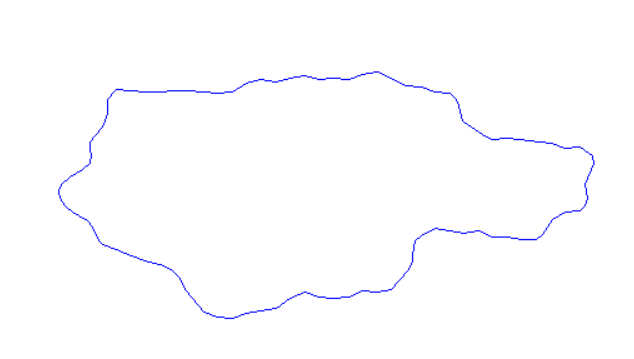
\includegraphics[width=0.6\linewidth,height=\textheight,keepaspectratio]{images/sdmTMB1.PNG}

}

\caption{Рис. 1.: Визуализация оболочки съемок}

\end{figure}%

\begin{Shaded}
\begin{Highlighting}[]
\CommentTok{\# Визуализация оболочки и точек съемок 2019{-}2024}
\FunctionTok{points}\NormalTok{(data}\SpecialCharTok{$}\NormalTok{xkm, data}\SpecialCharTok{$}\NormalTok{ykm, }\AttributeTok{pch=}\DecValTok{1}\NormalTok{, }\AttributeTok{cex=}\FloatTok{0.55}\NormalTok{,}\AttributeTok{col=}\StringTok{"black"}\NormalTok{)}
\end{Highlighting}
\end{Shaded}

\begin{figure}[H]

{\centering 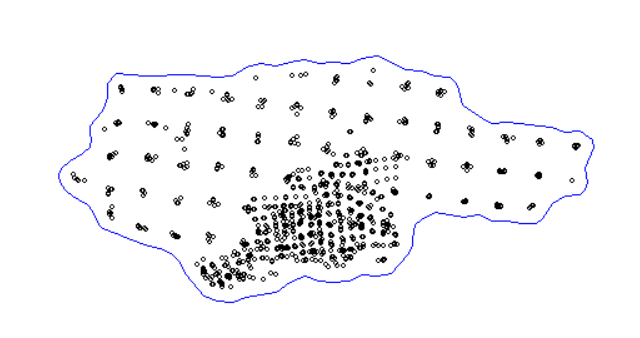
\includegraphics[width=0.6\linewidth,height=\textheight,keepaspectratio]{images/sdmTMB2.PNG}

}

\caption{Рис. 2.: Визуализация оболочки и точек съемок}

\end{figure}%

\begin{Shaded}
\begin{Highlighting}[]
\CommentTok{\# Фильтрация сетки: оставляем только точки внутри оболочки}
\NormalTok{line }\OtherTok{\textless{}{-}}\NormalTok{ Hull}\SpecialCharTok{$}\NormalTok{loc[, }\DecValTok{1}\SpecialCharTok{:}\DecValTok{2}\NormalTok{] }\SpecialCharTok{\%\textgreater{}\%} \FunctionTok{as.data.frame}\NormalTok{()}
\FunctionTok{colnames}\NormalTok{(line) }\OtherTok{\textless{}{-}} \FunctionTok{c}\NormalTok{(}\StringTok{"X"}\NormalTok{, }\StringTok{"Y"}\NormalTok{)}
\NormalTok{GRID}\SpecialCharTok{$}\NormalTok{AREA }\OtherTok{\textless{}{-}} \FunctionTok{point.in.polygon}\NormalTok{(GRID}\SpecialCharTok{$}\NormalTok{X, GRID}\SpecialCharTok{$}\NormalTok{Y, line}\SpecialCharTok{$}\NormalTok{X, line}\SpecialCharTok{$}\NormalTok{Y)}
\NormalTok{GRID }\OtherTok{\textless{}{-}}\NormalTok{ GRID[GRID}\SpecialCharTok{$}\NormalTok{AREA }\SpecialCharTok{\textgreater{}} \FloatTok{0.1}\NormalTok{, }\FunctionTok{c}\NormalTok{(}\StringTok{"X"}\NormalTok{, }\StringTok{"Y"}\NormalTok{)]  }\CommentTok{\# Только внутренние точки}

\CommentTok{\# {-}{-}{-}{-}{-}{-}{-}{-}{-}{-}{-}{-}{-}{-}{-}{-}{-}{-}{-}{-}{-}{-}{-}{-}{-}{-}{-}{-}{-}{-}{-}{-}{-}{-}{-}{-}{-}{-}{-}{-}{-}{-}{-}{-}{-}{-}{-}{-}{-}}
\CommentTok{\# 6. ПОДГОТОВКА СЕТКИ ДЛЯ ПРОГНОЗИРОВАНИЯ}
\CommentTok{\# {-}{-}{-}{-}{-}{-}{-}{-}{-}{-}{-}{-}{-}{-}{-}{-}{-}{-}{-}{-}{-}{-}{-}{-}{-}{-}{-}{-}{-}{-}{-}{-}{-}{-}{-}{-}{-}{-}{-}{-}{-}{-}{-}{-}{-}{-}{-}{-}{-}}

\CommentTok{\# Создание временной сетки (для каждого года)}
\NormalTok{grid }\OtherTok{\textless{}{-}} \FunctionTok{replicate\_df}\NormalTok{(GRID, }\StringTok{"YEAR"}\NormalTok{, }\FunctionTok{unique}\NormalTok{(data}\SpecialCharTok{$}\NormalTok{YEAR))}
\FunctionTok{colnames}\NormalTok{(grid) }\OtherTok{\textless{}{-}} \FunctionTok{c}\NormalTok{(}\StringTok{"xkm"}\NormalTok{, }\StringTok{"ykm"}\NormalTok{, }\StringTok{"YEAR"}\NormalTok{)}
\NormalTok{grid}\SpecialCharTok{$}\NormalTok{SURV }\OtherTok{\textless{}{-}} \StringTok{"CRAB"}  \CommentTok{\# Добавляем информацию о типе съемки}

\CommentTok{\# Визуализация оболочки и сетки для прогнозирования (grid)}
 \FunctionTok{plot}\NormalTok{(Hull)}
 \FunctionTok{points}\NormalTok{(grid}\SpecialCharTok{$}\NormalTok{xkm, grid}\SpecialCharTok{$}\NormalTok{ykm, }\AttributeTok{pch=}\DecValTok{1}\NormalTok{, }\AttributeTok{cex=}\FloatTok{0.55}\NormalTok{,}\AttributeTok{col=}\StringTok{"black"}\NormalTok{)}
\end{Highlighting}
\end{Shaded}

\begin{figure}[H]

{\centering 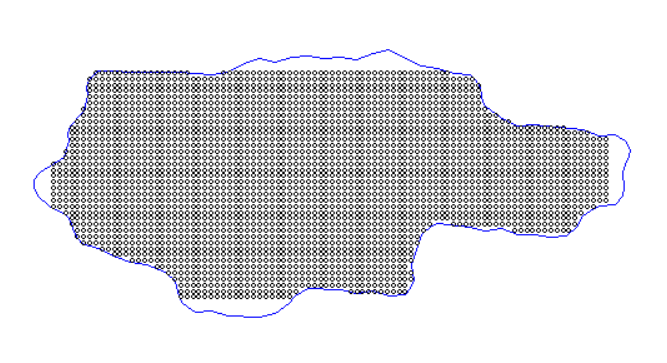
\includegraphics[width=0.6\linewidth,height=\textheight,keepaspectratio]{images/sdmTMB3.PNG}

}

\caption{Рис. 3.: Визуализация оболочки и сетки для прогнозирования
(grid)}

\end{figure}%

\begin{Shaded}
\begin{Highlighting}[]
\CommentTok{\# {-}{-}{-}{-}{-}{-}{-}{-}{-}{-}{-}{-}{-}{-}{-}{-}{-}{-}{-}{-}{-}{-}{-}{-}{-}{-}{-}{-}{-}{-}{-}{-}{-}{-}{-}{-}{-}{-}{-}{-}{-}{-}{-}{-}{-}{-}{-}{-}{-}{-}{-}}
\CommentTok{\# 7. ПОСТРОЕНИЕ ПРОСТРАНСТВЕННОЙ СЕТКИ (MESH)}
\CommentTok{\# {-}{-}{-}{-}{-}{-}{-}{-}{-}{-}{-}{-}{-}{-}{-}{-}{-}{-}{-}{-}{-}{-}{-}{-}{-}{-}{-}{-}{-}{-}{-}{-}{-}{-}{-}{-}{-}{-}{-}{-}{-}{-}{-}{-}{-}{-}{-}{-}{-}{-}{-}}

\CommentTok{\# Создание треугольной сетки для пространственного моделирования}
\NormalTok{mesh\_sdm }\OtherTok{\textless{}{-}} \FunctionTok{make\_mesh}\NormalTok{(}
\NormalTok{  data, }
  \FunctionTok{c}\NormalTok{(}\StringTok{"xkm"}\NormalTok{, }\StringTok{"ykm"}\NormalTok{),  }\CommentTok{\# Координаты}
  \AttributeTok{cutoff =} \DecValTok{10}        \CommentTok{\# Минимальное расстояние между узлами (км)}
\NormalTok{)}

\CommentTok{\# Визуализация сетки }
 \FunctionTok{plot}\NormalTok{(mesh\_sdm)}
\end{Highlighting}
\end{Shaded}

\begin{figure}[H]

{\centering 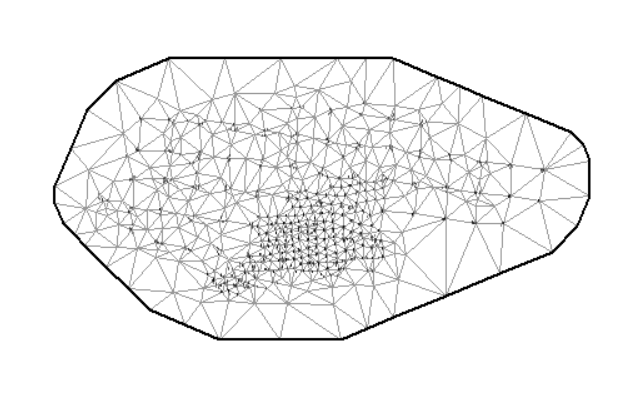
\includegraphics[width=0.6\linewidth,height=\textheight,keepaspectratio]{images/sdmTMB4.PNG}

}

\caption{Рис. 4.: Визуализация сетки (mesh)}

\end{figure}%

\begin{Shaded}
\begin{Highlighting}[]
\CommentTok{\# {-}{-}{-}{-}{-}{-}{-}{-}{-}{-}{-}{-}{-}{-}{-}{-}{-}{-}{-}{-}{-}{-}{-}{-}{-}{-}{-}{-}{-}{-}{-}{-}{-}{-}{-}{-}{-}{-}{-}{-}{-}{-}{-}{-}{-}{-}{-}{-}{-}{-}{-}}
\CommentTok{\# 8. ПОСТРОЕНИЕ ПРОСТРАНСТВЕННО{-}ВРЕМЕННОЙ МОДЕЛИ}
\CommentTok{\# {-}{-}{-}{-}{-}{-}{-}{-}{-}{-}{-}{-}{-}{-}{-}{-}{-}{-}{-}{-}{-}{-}{-}{-}{-}{-}{-}{-}{-}{-}{-}{-}{-}{-}{-}{-}{-}{-}{-}{-}{-}{-}{-}{-}{-}{-}{-}{-}{-}{-}{-}}

\NormalTok{m }\OtherTok{\textless{}{-}} \FunctionTok{sdmTMB}\NormalTok{(}
  \AttributeTok{data =}\NormalTok{ data, }
  \AttributeTok{formula =}\NormalTok{ Density }\SpecialCharTok{\textasciitilde{}} \DecValTok{0} \SpecialCharTok{+} \FunctionTok{as.factor}\NormalTok{(YEAR),  }\CommentTok{\# Формула: плотность зависит от года}
  \AttributeTok{time =} \StringTok{"YEAR"}\NormalTok{,         }\CommentTok{\# Временная переменная}
  \AttributeTok{mesh =}\NormalTok{ mesh\_sdm,       }\CommentTok{\# Пространственная сетка}
  \AttributeTok{family =} \FunctionTok{tweedie}\NormalTok{(}\AttributeTok{link =} \StringTok{"log"}\NormalTok{),  }\CommentTok{\# Статистическое распределение}
  \AttributeTok{spatial =} \StringTok{"on"}\NormalTok{,        }\CommentTok{\# Включение пространственных эффектов}
  \AttributeTok{spatiotemporal =} \StringTok{"iid"} \CommentTok{\# Пространственно{-}временные эффекты}
\NormalTok{)}

\CommentTok{\# Вывод результатов модели}
\FunctionTok{summary}\NormalTok{(m)}
\FunctionTok{AIC}\NormalTok{(m)  }\CommentTok{\# Критерий Акаике}
\FunctionTok{sanity}\NormalTok{(m)  }\CommentTok{\# Проверка корректности модели}
\end{Highlighting}
\end{Shaded}

Получили результаты:

\begin{Shaded}
\begin{Highlighting}[]
\SpecialCharTok{\textgreater{}} \CommentTok{\# Вывод результатов модели}
\ErrorTok{\textgreater{}} \FunctionTok{summary}\NormalTok{(m)}
\NormalTok{Spatiotemporal model fit by ML [}\StringTok{\textquotesingle{}sdmTMB\textquotesingle{}}\NormalTok{]}
\NormalTok{Formula}\SpecialCharTok{:}\NormalTok{ Density }\SpecialCharTok{\textasciitilde{}} \DecValTok{0} \SpecialCharTok{+} \FunctionTok{as.factor}\NormalTok{(YEAR)}
\NormalTok{Mesh}\SpecialCharTok{:} \FunctionTok{mesh\_sdm}\NormalTok{ (isotropic covariance)}
\NormalTok{Time column}\SpecialCharTok{:}\NormalTok{ YEAR}
\NormalTok{Data}\SpecialCharTok{:}\NormalTok{ data}
\NormalTok{Family}\SpecialCharTok{:} \FunctionTok{tweedie}\NormalTok{(}\AttributeTok{link =} \StringTok{\textquotesingle{}log\textquotesingle{}}\NormalTok{)}
 
\NormalTok{Conditional model}\SpecialCharTok{:}
\NormalTok{                    coef.est coef.se}
\FunctionTok{as.factor}\NormalTok{(YEAR)}\DecValTok{2019}     \FloatTok{2.15}    \FloatTok{0.72}
\FunctionTok{as.factor}\NormalTok{(YEAR)}\DecValTok{2020}     \FloatTok{1.49}    \FloatTok{0.76}
\FunctionTok{as.factor}\NormalTok{(YEAR)}\DecValTok{2021}     \FloatTok{1.74}    \FloatTok{0.76}
\FunctionTok{as.factor}\NormalTok{(YEAR)}\DecValTok{2022}     \FloatTok{1.62}    \FloatTok{0.73}
\FunctionTok{as.factor}\NormalTok{(YEAR)}\DecValTok{2023}     \FloatTok{1.50}    \FloatTok{0.74}
\FunctionTok{as.factor}\NormalTok{(YEAR)}\DecValTok{2024}     \FloatTok{1.56}    \FloatTok{0.72}

\NormalTok{Dispersion parameter}\SpecialCharTok{:} \FloatTok{19.71}
\NormalTok{Tweedie p}\SpecialCharTok{:} \FloatTok{1.50}
\NormalTok{Matern range}\SpecialCharTok{:} \FloatTok{142.65}
\NormalTok{Spatial SD}\SpecialCharTok{:} \FloatTok{2.01}
\NormalTok{Spatiotemporal IID SD}\SpecialCharTok{:} \FloatTok{0.95}
\NormalTok{ML criterion at convergence}\SpecialCharTok{:} \FloatTok{5984.224}

\NormalTok{See ?tidy.sdmTMB to extract these values as a data frame.}
\SpecialCharTok{\textgreater{}} \FunctionTok{AIC}\NormalTok{(m)  }\CommentTok{\# Критерий Акаике}
\NormalTok{[}\DecValTok{1}\NormalTok{] }\FloatTok{11990.45}
\SpecialCharTok{\textgreater{}} \FunctionTok{sanity}\NormalTok{(m)  }\CommentTok{\# Проверка корректности модели}
\NormalTok{v Non}\SpecialCharTok{{-}}\NormalTok{linear minimizer suggests successful convergence}
\NormalTok{v Hessian matrix is positive definite}
\NormalTok{v No extreme or very small eigenvalues detected}
\NormalTok{v No gradients with respect to fixed effects are }\SpecialCharTok{\textgreater{}=} \FloatTok{0.001}
\NormalTok{v No fixed}\SpecialCharTok{{-}}\NormalTok{effect standard errors are }\ConstantTok{NA}
\NormalTok{v No standard errors look unreasonably large}
\NormalTok{v No sigma parameters are }\SpecialCharTok{\textless{}} \FloatTok{0.01}
\NormalTok{v No sigma parameters are }\SpecialCharTok{\textgreater{}} \DecValTok{100}
\NormalTok{v Range parameter doesn}\StringTok{\textquotesingle{}t look unreasonably large}
\end{Highlighting}
\end{Shaded}

\subsubsection{\texorpdfstring{\textbf{Годовые
эффекты:}}{Годовые эффекты:}}\label{ux433ux43eux434ux43eux432ux44bux435-ux44dux444ux444ux435ux43aux442ux44b}

\begin{verbatim}
2019: 2.15 ± 0.72 → exp(2.15) ≈ 8.58 экз./км²
2020: 1.49 ± 0.76 → exp(1.49) ≈ 4.44 экз./км²
2024: 1.56 ± 0.72 → exp(1.56) ≈ 4.76 экз./км²
\end{verbatim}

\begin{itemize}
\item
  \textbf{2019 год} - пик запаса (8.58 экз./км²)
\item
  \textbf{2020 год} - резкое снижение (-52\% к 2019)
\item
  \textbf{2021-2024} - стабилизация на уровне \textasciitilde4.5-5.0
  экз./км²
\item
  \textbf{Стандартные ошибки} \textasciitilde0.75:

  \begin{itemize}
  \item
    Приемлемая точность для данных такого объема
  \item
    Все годовые оценки статистически значимы
  \end{itemize}

  Модель пространственно-временного распределения плотности камчатского
  краба успешно прошла все диагностические проверки, демонстрируя
  отличную сходимость и статистическую надежность. Параметр
  распределения Твиди (p=1.50) оптимально соответствует данным траловых
  съемок, учитывая характерную для уловов передисперсию и избыток
  нулевых значений.

  Годовые оценки показывают выраженную динамику запаса: в 2019 году
  зафиксирован пик плотности (8.58 экз./км²), после чего в 2020 году
  произошло резкое снижение до 4.44 экз./км². В последующие годы
  (2021-2024) плотность стабилизировалась на уровне 4.5-5.0 экз./км²,
  что составляет примерно 55\% от максимальных значений 2019 года.
  Стандартные ошибки годовых коэффициентов (0.72-0.76) свидетельствуют о
  хорошей точности оценок при текущем объеме данных.

  Пространственная структура распределения характеризуется
  крупномасштабными скоплениями с диапазоном корреляции 143 км (Matern
  range: 142.65), что согласуется с известными особенностями миграций
  камчатского краба. Высокое значение пространственной изменчивости
  (SD=2.01) отражает типичную для вида мозаичность распределения, где
  участки высокой плотности соседствуют с зонами отсутствия особей.
  Умеренная пространственно-временная изменчивость (IID SD=0.95)
  указывает на относительную стабильность пространственной структуры
  запаса между годами.

  Параметр дисперсии (19.71) подтверждает ожидаемо высокую
  вариабельность данных, характерную для траловых съемок морских
  гидробионтов. Полученные результаты надежно фиксируют значительное
  сокращение запаса после 2019 года с последующей стабилизацией на
  пониженном уровне.

  \subsection{\texorpdfstring{\textbf{Пояснение результатов
  \texttt{sanity(m)} для начинающих гидробиологов (от
  DeepSeek):}}{Пояснение результатов sanity(m) для начинающих гидробиологов (от DeepSeek):}}\label{ux43fux43eux44fux441ux43dux435ux43dux438ux435-ux440ux435ux437ux443ux43bux44cux442ux430ux442ux43eux432-sanitym-ux434ux43bux44f-ux43dux430ux447ux438ux43dux430ux44eux449ux438ux445-ux433ux438ux434ux440ux43eux431ux438ux43eux43bux43eux433ux43eux432-ux43eux442-deepseek}

  \textbf{1.
  \texttt{v\ Non-linear\ minimizer\ suggests\ successful\ convergence}}\\
  (Нелинейный оптимизатор успешно сошелся)\\
  \emph{Пояснение:} Алгоритм поиска параметров модели корректно завершил
  работу. Это значит, что модель ``научилась'' описывать ваши данные и
  не застряла в промежуточных вычислениях. Как если бы вы успешно
  завершили лабораторный анализ без технических сбоев.

  \textbf{2. \texttt{v\ Hessian\ matrix\ is\ positive\ definite}}\\
  (Матрица Гессе положительно определена)\\
  \emph{Пояснение:} Математическое подтверждение, что найденные
  параметры модели действительно оптимальны. Аналогично тому, как в
  микроскопии вы видите четкий фокус - здесь модель ``четко видит''
  закономерности в данных.

  \textbf{3.
  \texttt{v\ No\ extreme\ or\ very\ small\ eigenvalues\ detected}}\\
  (Не обнаружено экстремальных или очень маленьких собственных
  значений)\\
  \emph{Пояснение:} Модель статистически стабильна. Представьте, что вы
  измеряете длину рыб - если бы ваш штангенциркуль иногда показывал 0
  или 1000 мм, это было бы проблемой. Здесь аналогично - вычисления
  надежны.

  \textbf{4.
  \texttt{v\ No\ gradients\ with\ respect\ to\ fixed\ effects\ are\ \textgreater{}=\ 0.001}}\\
  (Градиенты для фиксированных эффектов \textless{} 0.001)\\
  \emph{Пояснение:} Все ключевые параметры модели (например, влияние
  года на плотность) рассчитаны точно. Это как убедиться, что все
  измерения в вашем эксперименте выполнены с требуемой точностью (±0.1
  мг, ±1 см и т.д.).

  \textbf{5. \texttt{v\ No\ fixed-effect\ standard\ errors\ are\ NA}}\\
  (Стандартные ошибки для фиксированных эффектов не отсутствуют)\\
  \emph{Пояснение:} Для каждого рассчитанного параметра (например,
  годовых оценок) указана погрешность. Важно как в химическом анализе -
  если для концентрации вещества нет погрешности, результат ненадежен.

  \textbf{6.
  \texttt{v\ No\ standard\ errors\ look\ unreasonably\ large}}\\
  (Стандартные ошибки выглядят разумными)\\
  \emph{Пояснение:} Погрешности оценок адекватны. Например, если
  плотность краба 5±1 экз./км² - это нормально, но 5±100 экз./км² было
  бы бессмысленным.

  \textbf{7.
  \texttt{v\ No\ sigma\ parameters\ are\ \textless{}\ 0.01}}\\
  (Параметры сигма не меньше 0.01)\\
  \emph{Пояснение:} Модель не игнорирует важные источники изменчивости.
  Аналогично тому, что в пробе воды вы не упустили бы важный показатель,
  сказав ``он слишком мал''.

  \textbf{8.
  \texttt{v\ No\ sigma\ parameters\ are\ \textgreater{}\ 100}}\\
  (Параметры сигма не превышают 100)\\
  \emph{Пояснение:} Модель не преувеличивает случайные вариации. Как
  если бы вы не приписали естественные колебания температуры воды
  катастрофическому изменению климата.

  \textbf{9.
  \texttt{v\ Range\ parameter\ doesn\textquotesingle{}t\ look\ unreasonably\ large}}\\
  (Параметр диапазона не выглядит чрезмерно большим)\\
  \emph{Пояснение:} Пространственная автокорреляция имеет биологически
  осмысленный масштаб. Например, если модель показала бы, что скопления
  краба одинаковы на расстоянии 1000 км - это было бы нереалистично.
\end{itemize}

\begin{Shaded}
\begin{Highlighting}[]
\CommentTok{\# {-}{-}{-}{-}{-}{-}{-}{-}{-}{-}{-}{-}{-}{-}{-}{-}{-}{-}{-}{-}{-}{-}{-}{-}{-}{-}{-}{-}{-}{-}{-}{-}{-}{-}{-}{-}{-}{-}{-}{-}{-}{-}{-}{-}{-}{-}{-}{-}{-}{-}{-}}
\CommentTok{\# 9. ДИАГНОСТИКА МОДЕЛИ}
\CommentTok{\# {-}{-}{-}{-}{-}{-}{-}{-}{-}{-}{-}{-}{-}{-}{-}{-}{-}{-}{-}{-}{-}{-}{-}{-}{-}{-}{-}{-}{-}{-}{-}{-}{-}{-}{-}{-}{-}{-}{-}{-}{-}{-}{-}{-}{-}{-}{-}{-}{-}{-}{-}}

\CommentTok{\# Расчет остатков модели}
\NormalTok{data}\SpecialCharTok{$}\NormalTok{resids }\OtherTok{\textless{}{-}} \FunctionTok{residuals}\NormalTok{(m) }

\CommentTok{\# Гистограмма остатков}
\FunctionTok{hist}\NormalTok{(data}\SpecialCharTok{$}\NormalTok{resids)}

\CommentTok{\# График квантиль{-}квантиль}
\FunctionTok{qqnorm}\NormalTok{(data}\SpecialCharTok{$}\NormalTok{resids)}
\FunctionTok{abline}\NormalTok{(}\AttributeTok{a =} \DecValTok{0}\NormalTok{, }\AttributeTok{b =} \DecValTok{1}\NormalTok{)}
\end{Highlighting}
\end{Shaded}

\begin{figure}[H]

{\centering 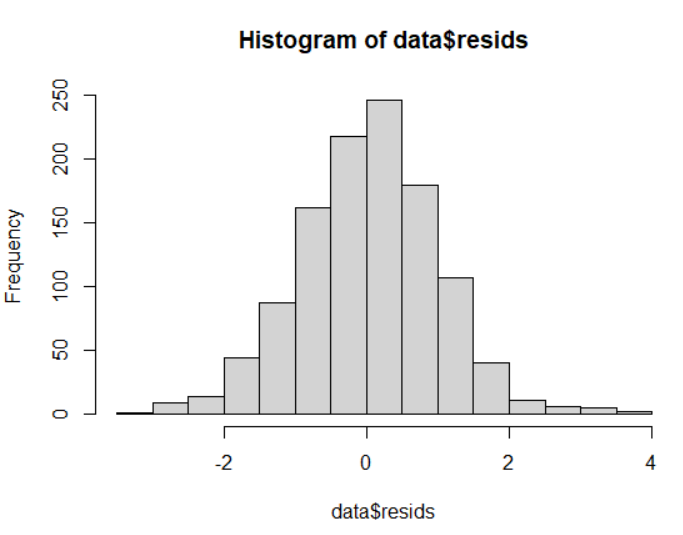
\includegraphics[width=0.6\linewidth,height=\textheight,keepaspectratio]{images/sdmTMB5.PNG}

}

\caption{Рис. 5.: Гистограмма остатков}

\end{figure}%

\begin{figure}[H]

{\centering 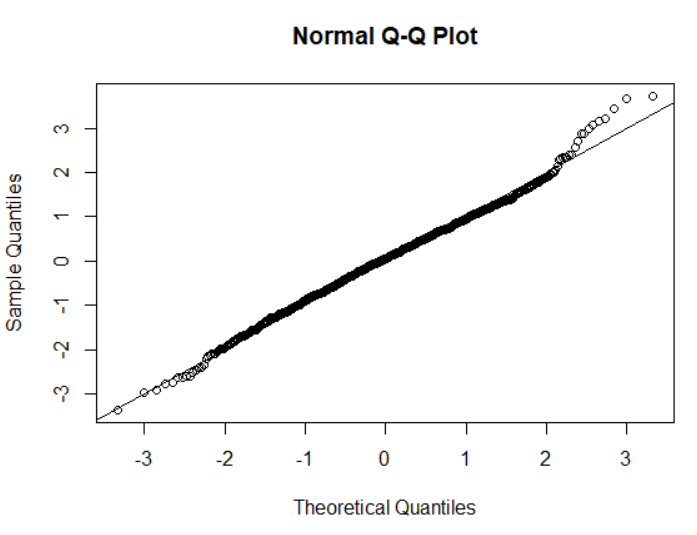
\includegraphics[width=0.6\linewidth,height=\textheight,keepaspectratio]{images/sdmTMB6.PNG}

}

\caption{Рис. 6.: График квантиль-квантиль}

\end{figure}%

\begin{Shaded}
\begin{Highlighting}[]
\CommentTok{\# {-}{-}{-}{-}{-}{-}{-}{-}{-}{-}{-}{-}{-}{-}{-}{-}{-}{-}{-}{-}{-}{-}{-}{-}{-}{-}{-}{-}{-}{-}{-}{-}{-}{-}{-}{-}{-}{-}{-}{-}{-}{-}{-}{-}{-}{-}{-}{-}{-}{-}{-}}
\CommentTok{\# 10. ПРОГНОЗИРОВАНИЕ НА СЕТКЕ}
\CommentTok{\# {-}{-}{-}{-}{-}{-}{-}{-}{-}{-}{-}{-}{-}{-}{-}{-}{-}{-}{-}{-}{-}{-}{-}{-}{-}{-}{-}{-}{-}{-}{-}{-}{-}{-}{-}{-}{-}{-}{-}{-}{-}{-}{-}{-}{-}{-}{-}{-}{-}{-}{-}}

\CommentTok{\# Прогноз значений плотности на сетке}
\NormalTok{predictions }\OtherTok{\textless{}{-}} \FunctionTok{predict}\NormalTok{(m, }\AttributeTok{newdata =}\NormalTok{ grid, }\AttributeTok{return\_tmb\_object =} \ConstantTok{TRUE}\NormalTok{)}
\NormalTok{RASP }\OtherTok{\textless{}{-}}\NormalTok{ predictions}\SpecialCharTok{$}\NormalTok{data}

\CommentTok{\# Преобразование координат обратно в широту/долготу}
\NormalTok{RASP}\SpecialCharTok{$}\NormalTok{xkm\_m }\OtherTok{\textless{}{-}}\NormalTok{ RASP}\SpecialCharTok{$}\NormalTok{xkm }\SpecialCharTok{*} \DecValTok{1000}  \CommentTok{\# Обратно в метры}
\NormalTok{RASP}\SpecialCharTok{$}\NormalTok{ykm\_m }\OtherTok{\textless{}{-}}\NormalTok{ RASP}\SpecialCharTok{$}\NormalTok{ykm }\SpecialCharTok{*} \DecValTok{1000}

\CommentTok{\# Создание пространственного объекта в UTM}
\NormalTok{utm\_proj }\OtherTok{\textless{}{-}} \FunctionTok{CRS}\NormalTok{(}\StringTok{"+proj=utm +zone=37 +datum=WGS84 +units=m +no\_defs"}\NormalTok{)}
\NormalTok{coords }\OtherTok{\textless{}{-}} \FunctionTok{cbind}\NormalTok{(RASP}\SpecialCharTok{$}\NormalTok{xkm\_m, RASP}\SpecialCharTok{$}\NormalTok{ykm\_m)}
\NormalTok{sp\_points }\OtherTok{\textless{}{-}} \FunctionTok{SpatialPoints}\NormalTok{(coords, }\AttributeTok{proj4string =}\NormalTok{ utm\_proj)}

\CommentTok{\# Преобразование в WGS84 (широта/долгота)}
\NormalTok{wgs84\_proj }\OtherTok{\textless{}{-}} \FunctionTok{CRS}\NormalTok{(}\StringTok{"+proj=longlat +datum=WGS84"}\NormalTok{)}
\NormalTok{sp\_points\_latlon }\OtherTok{\textless{}{-}} \FunctionTok{spTransform}\NormalTok{(sp\_points, wgs84\_proj)}

\CommentTok{\# Добавление координат в основной датафрейм}
\NormalTok{RASP}\SpecialCharTok{$}\NormalTok{X }\OtherTok{\textless{}{-}} \FunctionTok{coordinates}\NormalTok{(sp\_points\_latlon)[, }\DecValTok{1}\NormalTok{]  }\CommentTok{\# Долгота}
\NormalTok{RASP}\SpecialCharTok{$}\NormalTok{Y }\OtherTok{\textless{}{-}} \FunctionTok{coordinates}\NormalTok{(sp\_points\_latlon)[, }\DecValTok{2}\NormalTok{]  }\CommentTok{\# Широта}

\CommentTok{\# Удаление временных столбцов}
\NormalTok{RASP}\SpecialCharTok{$}\NormalTok{xkm\_m }\OtherTok{\textless{}{-}} \ConstantTok{NULL}
\NormalTok{RASP}\SpecialCharTok{$}\NormalTok{ykm\_m }\OtherTok{\textless{}{-}} \ConstantTok{NULL}

\CommentTok{\# Проверка структуры результата}
\FunctionTok{str}\NormalTok{(RASP)}

\CommentTok{\# {-}{-}{-}{-}{-}{-}{-}{-}{-}{-}{-}{-}{-}{-}{-}{-}{-}{-}{-}{-}{-}{-}{-}{-}{-}{-}{-}{-}{-}{-}{-}{-}{-}{-}{-}{-}{-}{-}{-}{-}{-}{-}{-}{-}{-}}
\CommentTok{\# 11. ВИЗУАЛИЗАЦИЯ РЕЗУЛЬТАТОВ (КАРТА)}
\CommentTok{\# {-}{-}{-}{-}{-}{-}{-}{-}{-}{-}{-}{-}{-}{-}{-}{-}{-}{-}{-}{-}{-}{-}{-}{-}{-}{-}{-}{-}{-}{-}{-}{-}{-}{-}{-}{-}{-}{-}{-}{-}{-}{-}{-}{-}{-}}

\CommentTok{\# Загрузка картографических данных}
\NormalTok{world }\OtherTok{\textless{}{-}} \FunctionTok{ne\_countries}\NormalTok{(}\AttributeTok{scale =} \StringTok{"medium"}\NormalTok{, }\AttributeTok{returnclass =} \StringTok{"sf"}\NormalTok{)}

\CommentTok{\# Определение региона интереса (Арктика России)}
\NormalTok{arctic\_bbox }\OtherTok{\textless{}{-}} \FunctionTok{st\_bbox}\NormalTok{(}\FunctionTok{c}\NormalTok{(}\AttributeTok{xmin =} \DecValTok{25}\NormalTok{, }\AttributeTok{xmax =} \DecValTok{70}\NormalTok{, }\AttributeTok{ymin =} \DecValTok{65}\NormalTok{, }\AttributeTok{ymax =} \DecValTok{80}\NormalTok{), }\AttributeTok{crs =} \DecValTok{4326}\NormalTok{)}
\NormalTok{arctic }\OtherTok{\textless{}{-}} \FunctionTok{st\_crop}\NormalTok{(world, arctic\_bbox)}

\CommentTok{\# Кастомные разрывы для цветовой шкалы}
\NormalTok{my\_breaks }\OtherTok{\textless{}{-}} \FunctionTok{c}\NormalTok{(}\FloatTok{0.001}\NormalTok{, }\FloatTok{0.1}\NormalTok{, }\DecValTok{1}\NormalTok{, }\DecValTok{200}\NormalTok{, }\DecValTok{10000}\NormalTok{)}

\CommentTok{\# Создание основной визуализации}
\FunctionTok{ggplot}\NormalTok{() }\SpecialCharTok{+}
  \CommentTok{\# Теплокарта плотности}
  \FunctionTok{geom\_point}\NormalTok{(}
    \AttributeTok{data =}\NormalTok{ RASP, }
    \FunctionTok{aes}\NormalTok{(}\AttributeTok{x =}\NormalTok{ X, }\AttributeTok{y =}\NormalTok{ Y, }\AttributeTok{color =} \FunctionTok{exp}\NormalTok{(est)), }
    \AttributeTok{size =} \FloatTok{0.8}\NormalTok{, }
    \AttributeTok{alpha =} \FloatTok{0.7}
\NormalTok{  ) }\SpecialCharTok{+} 
  \CommentTok{\# Наблюдаемые точки данных}
  \FunctionTok{geom\_point}\NormalTok{(}
    \AttributeTok{data =}\NormalTok{ data, }
    \FunctionTok{aes}\NormalTok{(}\AttributeTok{x =}\NormalTok{ X, }\AttributeTok{y =}\NormalTok{ Y, }\AttributeTok{size =}\NormalTok{ PROM), }\CommentTok{\# Размер по плотности}
    \AttributeTok{color =} \StringTok{"black"}\NormalTok{, }
    \AttributeTok{fill =} \ConstantTok{NA}\NormalTok{, }
    \AttributeTok{alpha =} \FloatTok{0.6}\NormalTok{,}
    \AttributeTok{shape =} \DecValTok{21} \CommentTok{\# Кружки с обводкой}
\NormalTok{  ) }\SpecialCharTok{+}
  \CommentTok{\# Картографическая подложка}
  \FunctionTok{geom\_sf}\NormalTok{(}\AttributeTok{data =}\NormalTok{ arctic, }\AttributeTok{fill =} \StringTok{"lightgrey"}\NormalTok{, }\AttributeTok{color =} \StringTok{"darkgrey"}\NormalTok{) }\SpecialCharTok{+}
  \CommentTok{\# Цветовая шкала (логарифмическая)}
  \FunctionTok{scale\_color\_viridis\_c}\NormalTok{(}
    \AttributeTok{name =} \StringTok{""}\NormalTok{,}
    \AttributeTok{option =} \StringTok{"H"}\NormalTok{, }
    \AttributeTok{trans =} \StringTok{"log"}\NormalTok{, }
    \AttributeTok{breaks =}\NormalTok{ my\_breaks, }
    \AttributeTok{labels =}\NormalTok{ my\_breaks}
\NormalTok{  ) }\SpecialCharTok{+}
  \CommentTok{\# Разделение по годам}
  \FunctionTok{facet\_wrap}\NormalTok{(}\SpecialCharTok{\textasciitilde{}}\NormalTok{ YEAR, }\AttributeTok{ncol =} \DecValTok{2}\NormalTok{) }\SpecialCharTok{+}
  \CommentTok{\# Настройка области просмотра}
  \FunctionTok{coord\_sf}\NormalTok{(}
    \AttributeTok{xlim =} \FunctionTok{c}\NormalTok{(}\FunctionTok{min}\NormalTok{(RASP}\SpecialCharTok{$}\NormalTok{X)}\SpecialCharTok{{-}}\DecValTok{1}\NormalTok{, }\FunctionTok{max}\NormalTok{(RASP}\SpecialCharTok{$}\NormalTok{X)}\SpecialCharTok{+}\DecValTok{1}\NormalTok{),}
    \AttributeTok{ylim =} \FunctionTok{c}\NormalTok{(}\FunctionTok{min}\NormalTok{(RASP}\SpecialCharTok{$}\NormalTok{Y)}\SpecialCharTok{{-}}\FloatTok{0.5}\NormalTok{, }\FunctionTok{max}\NormalTok{(RASP}\SpecialCharTok{$}\NormalTok{Y)}\SpecialCharTok{+}\FloatTok{0.5}\NormalTok{),}
    \AttributeTok{crs =} \DecValTok{4326}
\NormalTok{  ) }\SpecialCharTok{+}
  \CommentTok{\# Тема оформления}
  \FunctionTok{theme\_bw}\NormalTok{(}\AttributeTok{base\_size =} \DecValTok{12}\NormalTok{) }\SpecialCharTok{+}
  \FunctionTok{labs}\NormalTok{(}\AttributeTok{x =} \StringTok{"Долгота"}\NormalTok{, }\AttributeTok{y =} \StringTok{"Широта"}\NormalTok{, }\AttributeTok{title =} \StringTok{"Пространственное распределение плотности"}\NormalTok{) }\SpecialCharTok{+}
  \FunctionTok{theme}\NormalTok{(}
    \AttributeTok{panel.grid =} \FunctionTok{element\_line}\NormalTok{(}\AttributeTok{color =} \StringTok{"grey90"}\NormalTok{),}
    \AttributeTok{legend.position =} \StringTok{"bottom"}\NormalTok{,}
    \AttributeTok{legend.key.width =} \FunctionTok{unit}\NormalTok{(}\FloatTok{1.2}\NormalTok{, }\StringTok{"cm"}\NormalTok{),}
    \AttributeTok{strip.background =} \FunctionTok{element\_rect}\NormalTok{(}\AttributeTok{fill =} \StringTok{"white"}\NormalTok{)}
\NormalTok{  )}

\CommentTok{\# Сохранение графика (раскомментируйте)}
\CommentTok{\# ggsave("sdmTMBmap10.jpg", width = 8, height = 8, dpi = 300)}
\end{Highlighting}
\end{Shaded}

\begin{figure}[H]

{\centering 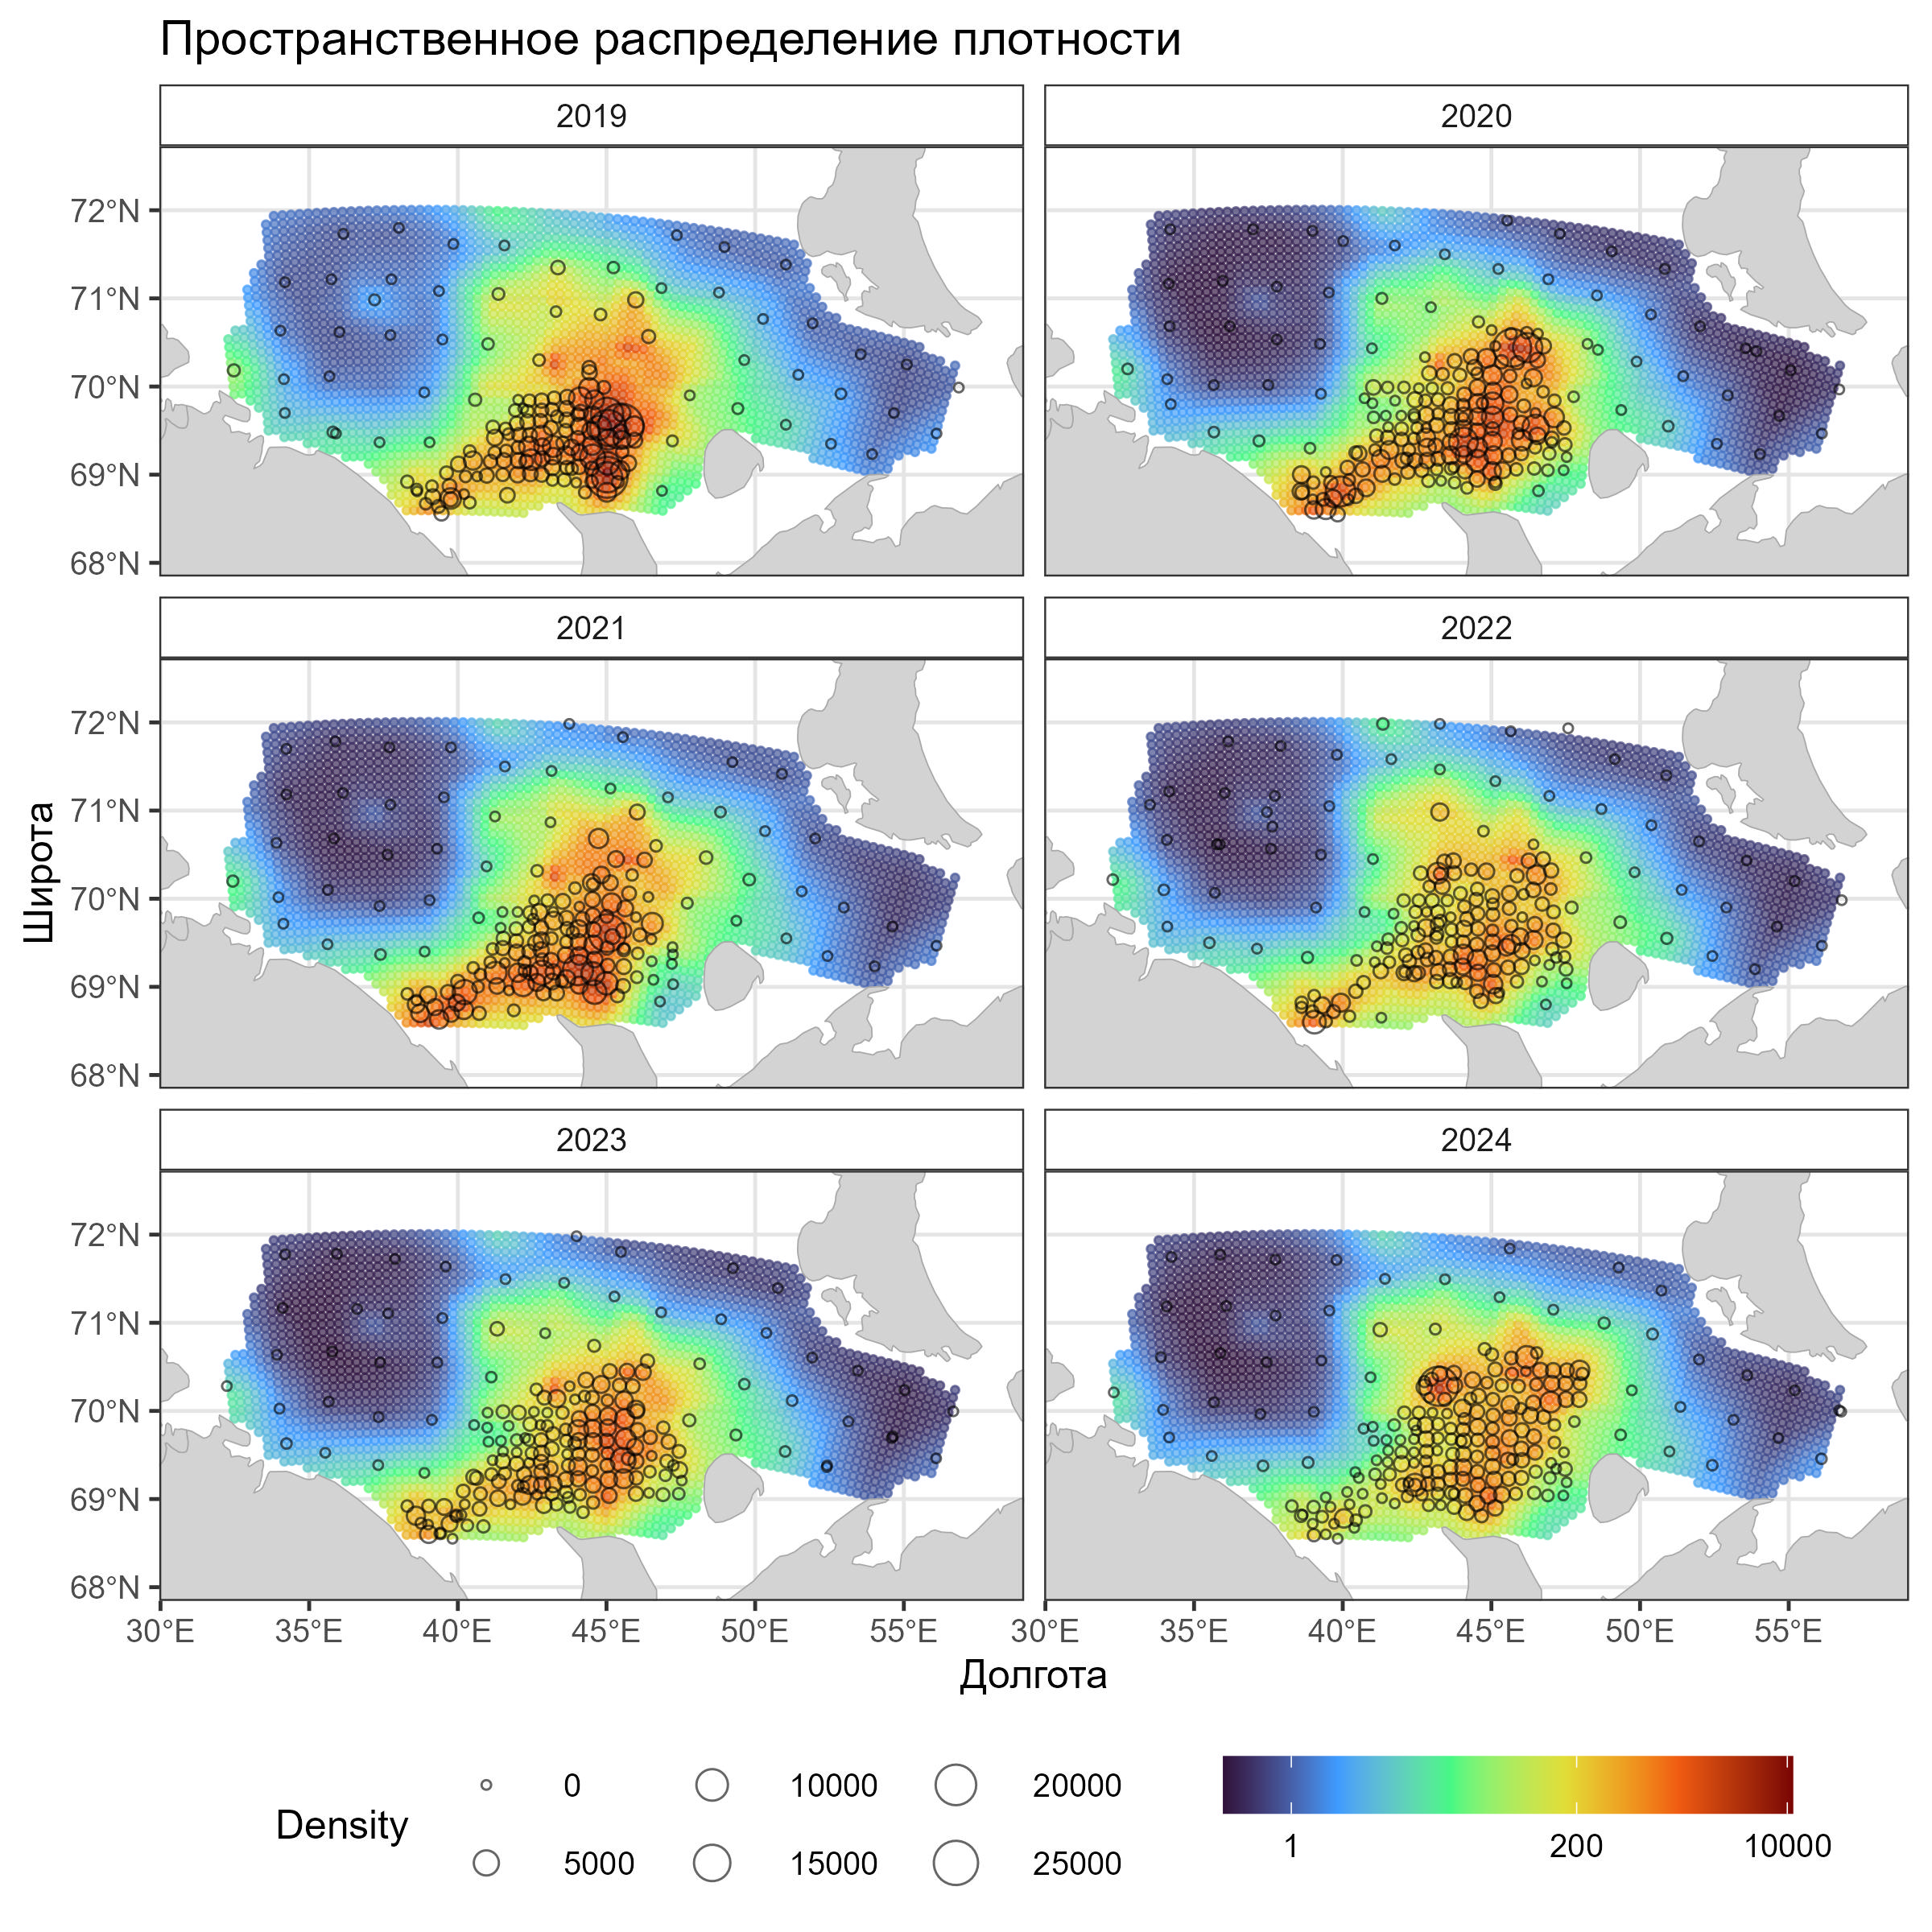
\includegraphics[width=0.9\linewidth,height=\textheight,keepaspectratio]{images/sdmTMBmap10.jpg}

}

\caption{Рис. 7.: Визуализация результатов (КАРТА)}

\end{figure}%

\begin{Shaded}
\begin{Highlighting}[]
\CommentTok{\# {-}{-}{-}{-}{-}{-}{-}{-}{-}{-}{-}{-}{-}{-}{-}{-}{-}{-}{-}{-}{-}{-}{-}{-}{-}{-}{-}{-}{-}{-}{-}{-}{-}{-}{-}{-}{-}{-}{-}{-}{-}{-}{-}{-}{-}{-}{-}{-}{-}{-}{-}}
\CommentTok{\# 12. РАСЧЕТ ИНДЕКСОВ ОБИЛИЯ}
\CommentTok{\# {-}{-}{-}{-}{-}{-}{-}{-}{-}{-}{-}{-}{-}{-}{-}{-}{-}{-}{-}{-}{-}{-}{-}{-}{-}{-}{-}{-}{-}{-}{-}{-}{-}{-}{-}{-}{-}{-}{-}{-}{-}{-}{-}{-}{-}{-}{-}{-}{-}{-}{-}}

\CommentTok{\# Расчет индексов с разными доверительными интервалами}
\NormalTok{index }\OtherTok{\textless{}{-}} \FunctionTok{get\_index}\NormalTok{(predictions, }\AttributeTok{area =} \DecValTok{4}\NormalTok{, }\AttributeTok{level =} \FloatTok{0.95}\NormalTok{, }\AttributeTok{bias\_correct =} \ConstantTok{TRUE}\NormalTok{)}
\NormalTok{index2 }\OtherTok{\textless{}{-}} \FunctionTok{get\_index}\NormalTok{(predictions, }\AttributeTok{area =} \DecValTok{4}\NormalTok{, }\AttributeTok{level =} \FloatTok{0.5}\NormalTok{, }\AttributeTok{bias\_correct =} \ConstantTok{TRUE}\NormalTok{)}

\CommentTok{\# Формирование сводной таблицы результатов}
\NormalTok{total }\OtherTok{\textless{}{-}} \FunctionTok{data.frame}\NormalTok{(}
  \AttributeTok{YEAR =}\NormalTok{ index}\SpecialCharTok{$}\NormalTok{YEAR,}
  \AttributeTok{lwr\_95 =}\NormalTok{ index}\SpecialCharTok{$}\NormalTok{lwr,}
  \AttributeTok{lwr\_50 =}\NormalTok{ index2}\SpecialCharTok{$}\NormalTok{lwr,}
  \AttributeTok{estimate =}\NormalTok{ index}\SpecialCharTok{$}\NormalTok{est,}
  \AttributeTok{upr\_50 =}\NormalTok{ index2}\SpecialCharTok{$}\NormalTok{upr,}
  \AttributeTok{upr\_95 =}\NormalTok{ index}\SpecialCharTok{$}\NormalTok{upr,}
  \AttributeTok{se =}\NormalTok{ index}\SpecialCharTok{$}\NormalTok{se,}
  \AttributeTok{cv =} \FunctionTok{sqrt}\NormalTok{(}\FunctionTok{exp}\NormalTok{(index}\SpecialCharTok{$}\NormalTok{se}\SpecialCharTok{\^{}}\DecValTok{2}\NormalTok{) }\SpecialCharTok{{-}} \DecValTok{1}\NormalTok{) }\CommentTok{\# Коэффициент вариации}
\NormalTok{)}

\CommentTok{\# Визуализация индексов обилия}
\FunctionTok{ggplot}\NormalTok{(total, }\FunctionTok{aes}\NormalTok{(}\AttributeTok{x =}\NormalTok{ YEAR, }\AttributeTok{y =}\NormalTok{ estimate}\SpecialCharTok{/}\DecValTok{1000000}\NormalTok{)) }\SpecialCharTok{+} 
  \CommentTok{\# Основная линия оценки}
  \FunctionTok{geom\_line}\NormalTok{(}\AttributeTok{linewidth =} \DecValTok{1}\NormalTok{, }\AttributeTok{color =} \StringTok{"steelblue"}\NormalTok{) }\SpecialCharTok{+}
  
  \CommentTok{\# 95\% доверительный интервал (более широкий и прозрачный)}
  \FunctionTok{geom\_ribbon}\NormalTok{(}
    \FunctionTok{aes}\NormalTok{(}\AttributeTok{ymin =}\NormalTok{ lwr\_95}\SpecialCharTok{/}\DecValTok{1000000}\NormalTok{, }\AttributeTok{ymax =}\NormalTok{ upr\_95}\SpecialCharTok{/}\DecValTok{1000000}\NormalTok{),}
    \AttributeTok{alpha =} \FloatTok{0.2}\NormalTok{,  }\CommentTok{\# Полупрозрачность}
    \AttributeTok{fill =} \StringTok{"steelblue"}\NormalTok{,}
    \AttributeTok{color =} \ConstantTok{NA}     \CommentTok{\# Без контура}
\NormalTok{  ) }\SpecialCharTok{+}
  
  \CommentTok{\# 50\% доверительный интервал (менее прозрачный)}
  \FunctionTok{geom\_ribbon}\NormalTok{(}
    \FunctionTok{aes}\NormalTok{(}\AttributeTok{ymin =}\NormalTok{ lwr\_50}\SpecialCharTok{/}\DecValTok{1000000}\NormalTok{, }\AttributeTok{ymax =}\NormalTok{ upr\_50}\SpecialCharTok{/}\DecValTok{1000000}\NormalTok{),}
    \AttributeTok{alpha =} \FloatTok{0.4}\NormalTok{,  }\CommentTok{\# Меньшая прозрачность}
    \AttributeTok{fill =} \StringTok{"steelblue"}\NormalTok{,}
    \AttributeTok{color =} \ConstantTok{NA}
\NormalTok{  ) }\SpecialCharTok{+}
  
  \CommentTok{\# Настройки осей и заголовков}
  \FunctionTok{ylab}\NormalTok{(}\StringTok{\textquotesingle{}Промысловый запас, млн. экз\textquotesingle{}}\NormalTok{) }\SpecialCharTok{+}
  \FunctionTok{xlab}\NormalTok{(}\StringTok{\textquotesingle{}Год\textquotesingle{}}\NormalTok{) }\SpecialCharTok{+}
  
  \CommentTok{\# Вертикальные линии для годов}
  \FunctionTok{geom\_vline}\NormalTok{(}
    \AttributeTok{xintercept =}\NormalTok{ total}\SpecialCharTok{$}\NormalTok{YEAR, }
    \AttributeTok{linetype =} \StringTok{"dotted"}\NormalTok{, }
    \AttributeTok{color =} \StringTok{"grey60"}\NormalTok{, }
    \AttributeTok{alpha =} \FloatTok{0.6}
\NormalTok{  ) }\SpecialCharTok{+}
  
  \CommentTok{\# Точки с значениями оценок}
  \FunctionTok{geom\_point}\NormalTok{(}
    \AttributeTok{size =} \DecValTok{3}\NormalTok{,}
    \AttributeTok{color =} \StringTok{"navyblue"}\NormalTok{,}
    \AttributeTok{fill =} \StringTok{"white"}\NormalTok{,}
    \AttributeTok{shape =} \DecValTok{21}
\NormalTok{  ) }\SpecialCharTok{+}
  
  \CommentTok{\# Настройка темы}
  \FunctionTok{theme\_minimal}\NormalTok{(}\AttributeTok{base\_size =} \DecValTok{14}\NormalTok{) }\SpecialCharTok{+}
  \FunctionTok{theme}\NormalTok{(}
    \AttributeTok{plot.title =} \FunctionTok{element\_text}\NormalTok{(}\AttributeTok{hjust =} \FloatTok{0.5}\NormalTok{, }\AttributeTok{face =} \StringTok{"bold"}\NormalTok{),}
    \AttributeTok{panel.grid.minor =} \FunctionTok{element\_blank}\NormalTok{(),}
    \AttributeTok{panel.grid.major =} \FunctionTok{element\_line}\NormalTok{(}\AttributeTok{color =} \StringTok{"grey90"}\NormalTok{),}
    \AttributeTok{axis.line =} \FunctionTok{element\_line}\NormalTok{(}\AttributeTok{color =} \StringTok{"grey30"}\NormalTok{),}
    \AttributeTok{legend.position =} \StringTok{"none"}
\NormalTok{  )}
\end{Highlighting}
\end{Shaded}

\begin{figure}[H]

{\centering 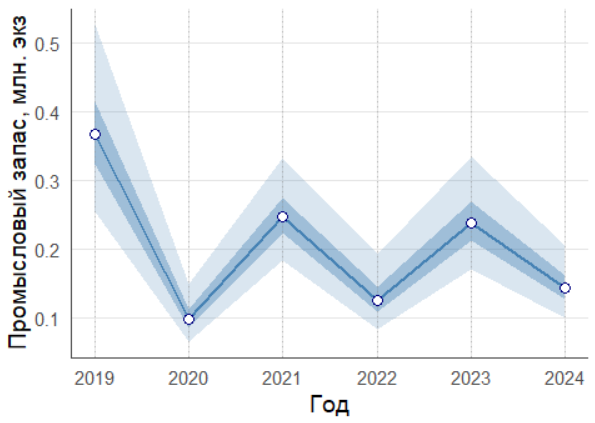
\includegraphics[width=0.6\linewidth,height=\textheight,keepaspectratio]{images/sdmTMB7.PNG}

}

\caption{Рис. 8.: Визуализация индексов обилия}

\end{figure}%

\begin{Shaded}
\begin{Highlighting}[]
\CommentTok{\# Форматированный вывод результатов}
\NormalTok{total }\SpecialCharTok{\%\textgreater{}\%} 
  \FunctionTok{mutate}\NormalTok{(}\AttributeTok{cv\_percent =} \DecValTok{100} \SpecialCharTok{*}\NormalTok{ cv) }\SpecialCharTok{\%\textgreater{}\%} 
  \FunctionTok{select}\NormalTok{(}
\NormalTok{    YEAR, }
\NormalTok{    estimate, }
\NormalTok{    lwr\_50,  }\CommentTok{\# Нижняя граница 50\% ДИ}
\NormalTok{    upr\_50,  }\CommentTok{\# Верхняя граница 50\% ДИ}
\NormalTok{    lwr\_95,  }\CommentTok{\# Нижняя граница 95\% ДИ}
\NormalTok{    upr\_95,  }\CommentTok{\# Верхняя граница 95\% ДИ}
\NormalTok{    cv\_percent}
\NormalTok{  ) }\SpecialCharTok{\%\textgreater{}\%}
\NormalTok{  knitr}\SpecialCharTok{::}\FunctionTok{kable}\NormalTok{(}
    \AttributeTok{format =} \StringTok{"pandoc"}\NormalTok{, }
    \AttributeTok{digits =} \FunctionTok{c}\NormalTok{(}\DecValTok{0}\NormalTok{, }\DecValTok{0}\NormalTok{, }\DecValTok{0}\NormalTok{, }\DecValTok{0}\NormalTok{, }\DecValTok{0}\NormalTok{, }\DecValTok{0}\NormalTok{, }\DecValTok{1}\NormalTok{),}
    \AttributeTok{col.names =} \FunctionTok{c}\NormalTok{(}
      \StringTok{"Год"}\NormalTok{, }
      \StringTok{"Оценка"}\NormalTok{, }
      \StringTok{"Нижняя 50\%"}\NormalTok{, }
      \StringTok{"Верхняя 50\%"}\NormalTok{, }
      \StringTok{"Нижняя 95\%"}\NormalTok{, }
      \StringTok{"Верхняя 95\%"}\NormalTok{, }
      \StringTok{"CV\%"}
\NormalTok{    )}
\NormalTok{  )}
\end{Highlighting}
\end{Shaded}

\begin{Shaded}
\begin{Highlighting}[]
\NormalTok{  Год    Оценка   Нижняя }\DecValTok{50}\SpecialCharTok{\%   Верхняя 50\%}\NormalTok{   Нижняя }\DecValTok{95}\SpecialCharTok{\%   Верхняя 95\%}\NormalTok{    CV\%}
\SpecialCharTok{{-}{-}{-}{-}{-}}  \SpecialCharTok{{-}{-}{-}{-}{-}{-}{-}{-}}  \SpecialCharTok{{-}{-}{-}{-}{-}{-}{-}{-}{-}{-}{-}}  \SpecialCharTok{{-}{-}{-}{-}{-}{-}{-}{-}{-}{-}{-}{-}}  \SpecialCharTok{{-}{-}{-}{-}{-}{-}{-}{-}{-}{-}{-}}  \SpecialCharTok{{-}{-}{-}{-}{-}{-}{-}{-}{-}{-}{-}{-}}  \SpecialCharTok{{-}{-}{-}{-}{-}}
 \DecValTok{2019}   \DecValTok{2381774}      \DecValTok{2177448}       \DecValTok{2605274}      \DecValTok{1835312}       \DecValTok{3090946}   \FloatTok{13.4}
 \DecValTok{2020}   \DecValTok{1634549}      \DecValTok{1539111}       \DecValTok{1735906}      \DecValTok{1372377}       \DecValTok{1946805}    \FloatTok{8.9}
 \DecValTok{2021}   \DecValTok{1920507}      \DecValTok{1794122}       \DecValTok{2055795}      \DecValTok{1575823}       \DecValTok{2340584}   \FloatTok{10.1}
 \DecValTok{2022}   \DecValTok{1036673}       \DecValTok{959251}       \DecValTok{1120344}       \DecValTok{827345}       \DecValTok{1298963}   \FloatTok{11.5}
 \DecValTok{2023}   \DecValTok{1147685}      \DecValTok{1068401}       \DecValTok{1232853}       \DecValTok{932147}       \DecValTok{1413062}   \FloatTok{10.6}
 \DecValTok{2024}   \DecValTok{1055733}       \DecValTok{985624}       \DecValTok{1130829}       \DecValTok{864640}       \DecValTok{1289060}   \FloatTok{10.2}
\SpecialCharTok{\textgreater{}} 
\end{Highlighting}
\end{Shaded}

\section{Базовая оценка +
предикторы}\label{ux431ux430ux437ux43eux432ux430ux44f-ux43eux446ux435ux43dux43aux430-ux43fux440ux435ux434ux438ux43aux442ux43eux440ux44b}

Сравнение пространственно-временных моделей sdmTMB с учетом типа съемки
(SURV) и года (YEAR)

Рассмотрим 4 пространственно-временные модели, оценивая их по:

Качеству подгонки (AIC) Стабильности оценок (sanity check) Значимости
ковариат Биологическому смыслу

4 модели: базовая модель, модель с глубиной (DEPTH),модель с
температурой (TEMP), модель с расстоянием до берега (DIST)

\begin{Shaded}
\begin{Highlighting}[]
\SpecialCharTok{\textgreater{}} \CommentTok{\# 8. ПОСТРОЕНИЕ ПРОСТРАНСТВЕННО{-}ВРЕМЕННОЙ МОДЕЛИ}
\ErrorTok{\textgreater{}} \CommentTok{\# {-}{-}{-}{-}{-}{-}{-}{-}{-}{-}{-}{-}{-}{-}{-}{-}{-}{-}{-}{-}{-}{-}{-}{-}{-}{-}{-}{-}{-}{-}{-}{-}{-}{-}{-}{-}{-}{-}{-}{-}{-}{-}{-}{-}{-}{-}{-}{-}{-}{-}{-}}
\ErrorTok{\textgreater{}} 
\ErrorTok{\textgreater{}}\NormalTok{ m }\OtherTok{\textless{}{-}} \FunctionTok{sdmTMB}\NormalTok{(}
\SpecialCharTok{+}   \AttributeTok{data =}\NormalTok{ data, }
\SpecialCharTok{+}   \AttributeTok{formula =}\NormalTok{ Density }\SpecialCharTok{\textasciitilde{}} \DecValTok{0}\SpecialCharTok{+} \FunctionTok{as.factor}\NormalTok{(SURV) }\SpecialCharTok{+} \FunctionTok{as.factor}\NormalTok{(YEAR),  }\CommentTok{\# Формула: плотность зависит от года}
\SpecialCharTok{+}   \AttributeTok{time =} \StringTok{"YEAR"}\NormalTok{,         }\CommentTok{\# Временная переменная}
\SpecialCharTok{+}   \AttributeTok{mesh =}\NormalTok{ mesh\_sdm,       }\CommentTok{\# Пространственная сетка}
\SpecialCharTok{+}   \AttributeTok{family =} \FunctionTok{tweedie}\NormalTok{(}\AttributeTok{link =} \StringTok{"log"}\NormalTok{),  }\CommentTok{\# Статистическое распределение}
\SpecialCharTok{+}   \AttributeTok{spatial =} \StringTok{"on"}\NormalTok{,        }\CommentTok{\# Включение пространственных эффектов}
\SpecialCharTok{+}   \AttributeTok{spatiotemporal =} \StringTok{"iid"} \CommentTok{\# Пространственно{-}временные эффекты}
\SpecialCharTok{+}\NormalTok{ )}
\SpecialCharTok{\textgreater{}} 
\ErrorTok{\textgreater{}} 
\ErrorTok{\textgreater{}} \CommentTok{\# Вывод результатов модели}
\ErrorTok{\textgreater{}} \FunctionTok{summary}\NormalTok{(m)}
\NormalTok{Spatiotemporal model fit by ML [}\StringTok{\textquotesingle{}sdmTMB\textquotesingle{}}\NormalTok{]}
\NormalTok{Formula}\SpecialCharTok{:}\NormalTok{ Density }\SpecialCharTok{\textasciitilde{}} \DecValTok{0} \SpecialCharTok{+} \FunctionTok{as.factor}\NormalTok{(SURV) }\SpecialCharTok{+} \FunctionTok{as.factor}\NormalTok{(YEAR)}
\NormalTok{Mesh}\SpecialCharTok{:} \FunctionTok{mesh\_sdm}\NormalTok{ (isotropic covariance)}
\NormalTok{Time column}\SpecialCharTok{:}\NormalTok{ YEAR}
\NormalTok{Data}\SpecialCharTok{:}\NormalTok{ data}
\NormalTok{Family}\SpecialCharTok{:} \FunctionTok{tweedie}\NormalTok{(}\AttributeTok{link =} \StringTok{\textquotesingle{}log\textquotesingle{}}\NormalTok{)}
 
\NormalTok{Conditional model}\SpecialCharTok{:}
\NormalTok{                    coef.est coef.se}
\FunctionTok{as.factor}\NormalTok{(SURV)CRAB     }\FloatTok{4.75}    \FloatTok{0.44}
\FunctionTok{as.factor}\NormalTok{(SURV)SUM      }\FloatTok{2.54}    \FloatTok{0.37}
\FunctionTok{as.factor}\NormalTok{(YEAR)}\DecValTok{2020}    \SpecialCharTok{{-}}\FloatTok{0.57}    \FloatTok{0.36}
\FunctionTok{as.factor}\NormalTok{(YEAR)}\DecValTok{2021}    \SpecialCharTok{{-}}\FloatTok{0.20}    \FloatTok{0.36}
\FunctionTok{as.factor}\NormalTok{(YEAR)}\DecValTok{2022}    \SpecialCharTok{{-}}\FloatTok{0.61}    \FloatTok{0.36}
\FunctionTok{as.factor}\NormalTok{(YEAR)}\DecValTok{2023}    \SpecialCharTok{{-}}\FloatTok{0.59}    \FloatTok{0.36}
\FunctionTok{as.factor}\NormalTok{(YEAR)}\DecValTok{2024}    \SpecialCharTok{{-}}\FloatTok{0.85}    \FloatTok{0.36}

\NormalTok{Dispersion parameter}\SpecialCharTok{:} \FloatTok{23.16}
\NormalTok{Tweedie p}\SpecialCharTok{:} \FloatTok{1.41}
\NormalTok{Matern range}\SpecialCharTok{:} \FloatTok{63.53}
\NormalTok{Spatial SD}\SpecialCharTok{:} \FloatTok{1.22}
\NormalTok{Spatiotemporal IID SD}\SpecialCharTok{:} \FloatTok{0.97}
\NormalTok{ML criterion at convergence}\SpecialCharTok{:} \FloatTok{5914.655}

\NormalTok{See ?tidy.sdmTMB to extract these values as a data frame.}
\SpecialCharTok{\textgreater{}} \FunctionTok{AIC}\NormalTok{(m)  }\CommentTok{\# Критерий Акаике}
\NormalTok{[}\DecValTok{1}\NormalTok{] }\FloatTok{11853.31}
\SpecialCharTok{\textgreater{}} \FunctionTok{sanity}\NormalTok{(m)  }\CommentTok{\# Проверка корректности модели}
\NormalTok{v Non}\SpecialCharTok{{-}}\NormalTok{linear minimizer suggests successful convergence}
\NormalTok{v Hessian matrix is positive definite}
\NormalTok{v No extreme or very small eigenvalues detected}
\NormalTok{v No gradients with respect to fixed effects are }\SpecialCharTok{\textgreater{}=} \FloatTok{0.001}
\NormalTok{v No fixed}\SpecialCharTok{{-}}\NormalTok{effect standard errors are }\ConstantTok{NA}
\NormalTok{v No standard errors look unreasonably large}
\NormalTok{v No sigma parameters are }\SpecialCharTok{\textless{}} \FloatTok{0.01}
\NormalTok{v No sigma parameters are }\SpecialCharTok{\textgreater{}} \DecValTok{100}
\NormalTok{v Range parameter doesn}\StringTok{\textquotesingle{}t look unreasonably large}
\StringTok{\textgreater{} }
\StringTok{\textgreater{} md \textless{}{-} sdmTMB(}
\StringTok{+   data = data, }
\StringTok{+   formula = Density \textasciitilde{} 0+ as.factor(SURV) + as.factor(YEAR)+s(DEPTH),  \# Формула: плотность зависит от года}
\StringTok{+   time = "YEAR",         \# Временная переменная}
\StringTok{+   mesh = mesh\_sdm,       \# Пространственная сетка}
\StringTok{+   family = tweedie(link = "log"),  \# Статистическое распределение}
\StringTok{+   spatial = "on",        \# Включение пространственных эффектов}
\StringTok{+   spatiotemporal = "iid" \# Пространственно{-}временные эффекты}
\StringTok{+ )}
\StringTok{\textgreater{} }
\StringTok{\textgreater{} }
\StringTok{\textgreater{} \# Вывод результатов модели}
\StringTok{\textgreater{} summary(md)}
\StringTok{Spatiotemporal model fit by ML [\textquotesingle{}}\NormalTok{sdmTMB}\StringTok{\textquotesingle{}]}
\StringTok{Formula: Density \textasciitilde{} 0 + as.factor(SURV) + as.factor(YEAR) + s(DEPTH)}
\StringTok{Mesh: mesh\_sdm (isotropic covariance)}
\StringTok{Time column: YEAR}
\StringTok{Data: data}
\StringTok{Family: tweedie(link = \textquotesingle{}}\NormalTok{log}\StringTok{\textquotesingle{})}
\StringTok{ }
\StringTok{Conditional model:}
\StringTok{                    coef.est coef.se}
\StringTok{as.factor(SURV)CRAB     5.42    0.32}
\StringTok{as.factor(SURV)SUM      3.09    0.28}
\StringTok{as.factor(YEAR)2020    {-}0.52    0.27}
\StringTok{as.factor(YEAR)2021    {-}0.15    0.27}
\StringTok{as.factor(YEAR)2022    {-}0.67    0.27}
\StringTok{as.factor(YEAR)2023    {-}0.63    0.27}
\StringTok{as.factor(YEAR)2024    {-}0.93    0.27}
\StringTok{sDEPTH                 {-}0.60    0.42}

\StringTok{Smooth terms:}
\StringTok{           Std. Dev.}
\StringTok{sds(DEPTH)      1.71}

\StringTok{Dispersion parameter: 24.43}
\StringTok{Tweedie p: 1.39}
\StringTok{Matern range: 40.20}
\StringTok{Spatial SD: 0.97}
\StringTok{Spatiotemporal IID SD: 0.94}
\StringTok{ML criterion at convergence: 5907.365}

\StringTok{See ?tidy.sdmTMB to extract these values as a data frame.}
\StringTok{\textgreater{} AIC(md)  \# Критерий Акаике}
\StringTok{[1] 11842.73}
\StringTok{\textgreater{} sanity(md)  \# Проверка корректности модели}
\StringTok{v Non{-}linear minimizer suggests successful convergence}
\StringTok{v Hessian matrix is positive definite}
\StringTok{v No extreme or very small eigenvalues detected}
\StringTok{v No gradients with respect to fixed effects are \textgreater{}= 0.001}
\StringTok{v No fixed{-}effect standard errors are NA}
\StringTok{v No standard errors look unreasonably large}
\StringTok{v No sigma parameters are \textless{} 0.01}
\StringTok{v No sigma parameters are \textgreater{} 100}
\StringTok{v Range parameter doesn\textquotesingle{}}\NormalTok{t look unreasonably large}
\SpecialCharTok{\textgreater{}} 
\ErrorTok{\textgreater{}} 
\ErrorTok{\textgreater{}}\NormalTok{ mt }\OtherTok{\textless{}{-}} \FunctionTok{sdmTMB}\NormalTok{(}
\SpecialCharTok{+}   \AttributeTok{data =}\NormalTok{ data, }
\SpecialCharTok{+}   \AttributeTok{formula =}\NormalTok{ Density }\SpecialCharTok{\textasciitilde{}} \DecValTok{0}\SpecialCharTok{+} \FunctionTok{as.factor}\NormalTok{(SURV) }\SpecialCharTok{+} \FunctionTok{as.factor}\NormalTok{(YEAR)}\SpecialCharTok{+}\FunctionTok{s}\NormalTok{(TEMP),  }\CommentTok{\# Формула: плотность зависит от года}
\SpecialCharTok{+}   \AttributeTok{time =} \StringTok{"YEAR"}\NormalTok{,         }\CommentTok{\# Временная переменная}
\SpecialCharTok{+}   \AttributeTok{mesh =}\NormalTok{ mesh\_sdm,       }\CommentTok{\# Пространственная сетка}
\SpecialCharTok{+}   \AttributeTok{family =} \FunctionTok{tweedie}\NormalTok{(}\AttributeTok{link =} \StringTok{"log"}\NormalTok{),  }\CommentTok{\# Статистическое распределение}
\SpecialCharTok{+}   \AttributeTok{spatial =} \StringTok{"on"}\NormalTok{,        }\CommentTok{\# Включение пространственных эффектов}
\SpecialCharTok{+}   \AttributeTok{spatiotemporal =} \StringTok{"iid"} \CommentTok{\# Пространственно{-}временные эффекты}
\SpecialCharTok{+}\NormalTok{ )}
\SpecialCharTok{\textgreater{}} 
\ErrorTok{\textgreater{}} 
\ErrorTok{\textgreater{}} \CommentTok{\# Вывод результатов модели}
\ErrorTok{\textgreater{}} \FunctionTok{summary}\NormalTok{(mt)}
\NormalTok{Spatiotemporal model fit by ML [}\StringTok{\textquotesingle{}sdmTMB\textquotesingle{}}\NormalTok{]}
\NormalTok{Formula}\SpecialCharTok{:}\NormalTok{ Density }\SpecialCharTok{\textasciitilde{}} \DecValTok{0} \SpecialCharTok{+} \FunctionTok{as.factor}\NormalTok{(SURV) }\SpecialCharTok{+} \FunctionTok{as.factor}\NormalTok{(YEAR) }\SpecialCharTok{+} \FunctionTok{s}\NormalTok{(TEMP)}
\NormalTok{Mesh}\SpecialCharTok{:} \FunctionTok{mesh\_sdm}\NormalTok{ (isotropic covariance)}
\NormalTok{Time column}\SpecialCharTok{:}\NormalTok{ YEAR}
\NormalTok{Data}\SpecialCharTok{:}\NormalTok{ data}
\NormalTok{Family}\SpecialCharTok{:} \FunctionTok{tweedie}\NormalTok{(}\AttributeTok{link =} \StringTok{\textquotesingle{}log\textquotesingle{}}\NormalTok{)}
 
\NormalTok{Conditional model}\SpecialCharTok{:}
\NormalTok{                    coef.est coef.se}
\FunctionTok{as.factor}\NormalTok{(SURV)CRAB     }\FloatTok{4.95}    \FloatTok{0.40}
\FunctionTok{as.factor}\NormalTok{(SURV)SUM      }\FloatTok{2.69}    \FloatTok{0.34}
\FunctionTok{as.factor}\NormalTok{(YEAR)}\DecValTok{2020}    \SpecialCharTok{{-}}\FloatTok{0.14}    \FloatTok{0.43}
\FunctionTok{as.factor}\NormalTok{(YEAR)}\DecValTok{2021}    \SpecialCharTok{{-}}\FloatTok{0.19}    \FloatTok{0.33}
\FunctionTok{as.factor}\NormalTok{(YEAR)}\DecValTok{2022}    \SpecialCharTok{{-}}\FloatTok{0.77}    \FloatTok{0.42}
\FunctionTok{as.factor}\NormalTok{(YEAR)}\DecValTok{2023}    \SpecialCharTok{{-}}\FloatTok{0.62}    \FloatTok{0.33}
\FunctionTok{as.factor}\NormalTok{(YEAR)}\DecValTok{2024}    \SpecialCharTok{{-}}\FloatTok{0.91}    \FloatTok{0.34}
\NormalTok{sTEMP                   }\FloatTok{0.80}    \FloatTok{0.83}

\NormalTok{Smooth terms}\SpecialCharTok{:}
\NormalTok{          Std. Dev.}
\FunctionTok{sds}\NormalTok{(TEMP)      }\FloatTok{3.15}

\NormalTok{Dispersion parameter}\SpecialCharTok{:} \FloatTok{23.42}
\NormalTok{Tweedie p}\SpecialCharTok{:} \FloatTok{1.40}
\NormalTok{Matern range}\SpecialCharTok{:} \FloatTok{55.04}
\NormalTok{Spatial SD}\SpecialCharTok{:} \FloatTok{1.12}
\NormalTok{Spatiotemporal IID SD}\SpecialCharTok{:} \FloatTok{0.96}
\NormalTok{ML criterion at convergence}\SpecialCharTok{:} \FloatTok{5912.795}

\NormalTok{See ?tidy.sdmTMB to extract these values as a data frame.}
\SpecialCharTok{\textgreater{}} \FunctionTok{AIC}\NormalTok{(mt)  }\CommentTok{\# Критерий Акаике}
\NormalTok{[}\DecValTok{1}\NormalTok{] }\FloatTok{11853.59}
\SpecialCharTok{\textgreater{}} \FunctionTok{sanity}\NormalTok{(mt)  }\CommentTok{\# Проверка корректности модели}
\NormalTok{v Non}\SpecialCharTok{{-}}\NormalTok{linear minimizer suggests successful convergence}
\NormalTok{v Hessian matrix is positive definite}
\NormalTok{v No extreme or very small eigenvalues detected}
\NormalTok{v No gradients with respect to fixed effects are }\SpecialCharTok{\textgreater{}=} \FloatTok{0.001}
\NormalTok{v No fixed}\SpecialCharTok{{-}}\NormalTok{effect standard errors are }\ConstantTok{NA}
\NormalTok{v No standard errors look unreasonably large}
\NormalTok{v No sigma parameters are }\SpecialCharTok{\textless{}} \FloatTok{0.01}
\NormalTok{v No sigma parameters are }\SpecialCharTok{\textgreater{}} \DecValTok{100}
\NormalTok{v Range parameter doesn}\StringTok{\textquotesingle{}t look unreasonably large}
\StringTok{\textgreater{} }
\StringTok{\textgreater{} mdist \textless{}{-} sdmTMB(}
\StringTok{+   data = data, }
\StringTok{+   formula = Density \textasciitilde{} 0+ as.factor(SURV) + as.factor(YEAR)+s(DIST),  \# Формула: плотность зависит от года}
\StringTok{+   time = "YEAR",         \# Временная переменная}
\StringTok{+   mesh = mesh\_sdm,       \# Пространственная сетка}
\StringTok{+   family = tweedie(link = "log"),  \# Статистическое распределение}
\StringTok{+   spatial = "on",        \# Включение пространственных эффектов}
\StringTok{+   spatiotemporal = "iid" \# Пространственно{-}временные эффекты}
\StringTok{+ )}
\StringTok{\textgreater{} }
\StringTok{\textgreater{} }
\StringTok{\textgreater{} \# Вывод результатов модели}
\StringTok{\textgreater{} summary(mdist)}
\StringTok{Spatiotemporal model fit by ML [\textquotesingle{}}\NormalTok{sdmTMB}\StringTok{\textquotesingle{}]}
\StringTok{Formula: Density \textasciitilde{} 0 + as.factor(SURV) + as.factor(YEAR) + s(DIST)}
\StringTok{Mesh: mesh\_sdm (isotropic covariance)}
\StringTok{Time column: YEAR}
\StringTok{Data: data}
\StringTok{Family: tweedie(link = \textquotesingle{}}\NormalTok{log}\StringTok{\textquotesingle{})}
\StringTok{ }
\StringTok{Conditional model:}
\StringTok{                    coef.est coef.se}
\StringTok{as.factor(SURV)CRAB     4.74    0.44}
\StringTok{as.factor(SURV)SUM      2.55    0.37}
\StringTok{as.factor(YEAR)2020    {-}0.57    0.36}
\StringTok{as.factor(YEAR)2021    {-}0.20    0.36}
\StringTok{as.factor(YEAR)2022    {-}0.61    0.36}
\StringTok{as.factor(YEAR)2023    {-}0.60    0.36}
\StringTok{as.factor(YEAR)2024    {-}0.85    0.36}
\StringTok{sDIST                  {-}0.06    0.16}

\StringTok{Smooth terms:}
\StringTok{          Std. Dev.}
\StringTok{sds(DIST)         0}

\StringTok{Dispersion parameter: 23.11}
\StringTok{Tweedie p: 1.41}
\StringTok{Matern range: 63.83}
\StringTok{Spatial SD: 1.22}
\StringTok{Spatiotemporal IID SD: 0.97}
\StringTok{ML criterion at convergence: 5914.594}

\StringTok{See ?tidy.sdmTMB to extract these values as a data frame.}

\StringTok{**Possible issues detected! Check output of sanity().**}
\StringTok{\textgreater{} AIC(mdist)  \# Критерий Акаике}
\StringTok{[1] 11857.19}
\StringTok{\textgreater{} sanity(mdist)  \# Проверка корректности модели}
\StringTok{v Non{-}linear minimizer suggests successful convergence}
\StringTok{v Hessian matrix is positive definite}
\StringTok{v No extreme or very small eigenvalues detected}
\StringTok{v No gradients with respect to fixed effects are \textgreater{}= 0.001}
\StringTok{v No fixed{-}effect standard errors are NA}
\StringTok{x \textasciigrave{}ln\_smooth\_sigma\textasciigrave{} standard error may be large}
\StringTok{i Try simplifying the model, adjusting the mesh, or adding priors}

\StringTok{v No sigma parameters are \textless{} 0.01}
\StringTok{v No sigma parameters are \textgreater{} 100}
\StringTok{v Range parameter doesn\textquotesingle{}}\NormalTok{t look unreasonably large}
\SpecialCharTok{\textgreater{}} 
\end{Highlighting}
\end{Shaded}

\subsubsection{\texorpdfstring{\textbf{1. Базовая модель (SURV +
YEAR)}}{1. Базовая модель (SURV + YEAR)}}\label{ux431ux430ux437ux43eux432ux430ux44f-ux43cux43eux434ux435ux43bux44c-surv-year}

\begin{verbatim}
Density ~ 0 + as.factor(SURV) + as.factor(YEAR)
\end{verbatim}

\begin{itemize}
\item
  \textbf{AIC}: 11853.31
\item
  \textbf{Проверка стабильности}: Все параметры стабильны
\item
  \textbf{Ключевые эффекты}:

  \begin{itemize}
  \item
    Высокая плотность в съемках CRAB (коэф. 4.75)
  \item
    Снижение плотности во всех годах относительно базового уровня
    (2020-2024: -0.57 до -0.85)
  \end{itemize}
\item
  \textbf{Пространственные параметры}:

  \begin{itemize}
  \item
    Диапазон Матерна: 63.53 км
  \item
    Пространственная SD: 1.22
  \end{itemize}
\end{itemize}

\subsubsection{\texorpdfstring{\textbf{2. Модель с глубиной
(DEPTH)}}{2. Модель с глубиной (DEPTH)}}\label{ux43cux43eux434ux435ux43bux44c-ux441-ux433ux43bux443ux431ux438ux43dux43eux439-depth}

\begin{verbatim}
Density ~ 0 + as.factor(SURV) + as.factor(YEAR) + s(DEPTH)
\end{verbatim}

\begin{itemize}
\item
  \textbf{AIC}: 11842.73 (наилучший)
\item
  \textbf{Проверка стабильности}: Все параметры стабильны
\item
  \textbf{Ключевые эффекты}:

  \begin{itemize}
  \item
    Сильное отрицательное влияние глубины (коэф. -0.60, SE=0.42)
  \item
    Усиление контраста между съемками CRAB/SUM (CRAB: 5.42 vs SUM: 3.09)
  \end{itemize}
\item
  \textbf{Улучшения}:

  \begin{itemize}
  \item
    Снижение AIC на 10.58 пунктов
  \item
    Уменьшение пространственного диапазона (40.20 км)
  \end{itemize}
\item
  \textbf{Интерпретация}: Глубина --- значимый экологический фактор
  распределения
\end{itemize}

\subsubsection{\texorpdfstring{\textbf{3. Модель с температурой
(TEMP)}}{3. Модель с температурой (TEMP)}}\label{ux43cux43eux434ux435ux43bux44c-ux441-ux442ux435ux43cux43fux435ux440ux430ux442ux443ux440ux43eux439-temp}

\begin{verbatim}
Density ~ 0 + as.factor(SURV) + as.factor(YEAR) + s(TEMP)
\end{verbatim}

\begin{itemize}
\item
  \textbf{AIC}: 11853.59 (хуже базовой)
\item
  \textbf{Проверка стабильности}: Стабильна, но высокий SE сглаживания
\item
  \textbf{Ключевые эффекты}:

  \begin{itemize}
  \item
    Слабый положительный эффект температуры (коэф. 0.80, SE=0.83)
  \item
    Незначительное изменение годовых эффектов
  \end{itemize}
\item
  \textbf{Проблемы}: Минимальное улучшение модели, высокая
  неопределенность эффекта температуры
\end{itemize}

\subsubsection{\texorpdfstring{\textbf{4. Модель с расстоянием
(DIST)}}{4. Модель с расстоянием (DIST)}}\label{ux43cux43eux434ux435ux43bux44c-ux441-ux440ux430ux441ux441ux442ux43eux44fux43dux438ux435ux43c-dist}

\begin{verbatim}
Density ~ 0 + as.factor(SURV) + as.factor(YEAR) + s(DIST)
\end{verbatim}

\begin{itemize}
\item
  \textbf{AIC}: 11857.19 (наихудший)
\item
  \textbf{Проверка стабильности}: Проблемы со сглаживанием
\item
  \textbf{Ключевые эффекты}:

  \begin{itemize}
  \item
    Незначительный эффект расстояния (коэф. -0.06, SE=0.16)
  \item
    Практически идентична базовой модели
  \end{itemize}
\item
  \textbf{Проблемы}: Наихудший AIC, предупреждения о нестабильности
\end{itemize}

\subsection{\texorpdfstring{\textbf{Сводка сравнения
моделей}}{Сводка сравнения моделей}}\label{ux441ux432ux43eux434ux43aux430-ux441ux440ux430ux432ux43dux435ux43dux438ux44f-ux43cux43eux434ux435ux43bux435ux439}

\begin{longtable}[]{@{}
  >{\raggedright\arraybackslash}p{(\linewidth - 10\tabcolsep) * \real{0.1667}}
  >{\raggedright\arraybackslash}p{(\linewidth - 10\tabcolsep) * \real{0.1667}}
  >{\raggedright\arraybackslash}p{(\linewidth - 10\tabcolsep) * \real{0.1667}}
  >{\raggedright\arraybackslash}p{(\linewidth - 10\tabcolsep) * \real{0.1667}}
  >{\raggedright\arraybackslash}p{(\linewidth - 10\tabcolsep) * \real{0.1667}}
  >{\raggedright\arraybackslash}p{(\linewidth - 10\tabcolsep) * \real{0.1667}}@{}}
\toprule\noalign{}
\begin{minipage}[b]{\linewidth}\raggedright
\textbf{Модель}
\end{minipage} & \begin{minipage}[b]{\linewidth}\raggedright
\textbf{AIC}
\end{minipage} & \begin{minipage}[b]{\linewidth}\raggedright
\textbf{ΔAIC}
\end{minipage} & \begin{minipage}[b]{\linewidth}\raggedright
\textbf{Стабильность}
\end{minipage} & \begin{minipage}[b]{\linewidth}\raggedright
\textbf{Ключевой предиктор}
\end{minipage} & \begin{minipage}[b]{\linewidth}\raggedright
\textbf{Эффект ковариаты}
\end{minipage} \\
\midrule\noalign{}
\endhead
\bottomrule\noalign{}
\endlastfoot
\textbf{DEPTH} & 11842.73 & - & ✓✓✓ & Глубина & Сильный (-0.60) \\
Базовая & 11853.31 & +10.6 & ✓✓✓ & - & - \\
TEMP & 11853.59 & +10.9 & ✓✓ & Температура & Слабый (+0.80) \\
DIST & 11857.19 & +14.5 & ✗ & Расстояние & Незначительный (-0.06) \\
\end{longtable}

\subsection{\texorpdfstring{\textbf{Рекомендации}}{Рекомендации}}\label{ux440ux435ux43aux43eux43cux435ux43dux434ux430ux446ux438ux438-1}

\begin{enumerate}
\def\labelenumi{\arabic{enumi}.}
\item
  \textbf{Лучшая модель}: С глубиной (DEPTH)

  \begin{itemize}
  \item
    Значительное улучшение AIC (-10.58)
  \item
    Биологически интерпретируемый эффект (глубина --- ключевой фактор
    распределения краба)
  \item
    Стабильные оценки параметров
  \end{itemize}
\item
  \textbf{Практическое значение}:

  \begin{itemize}
  \item
    Глубина объясняет \textasciitilde12\% пространственной
    вариабельности (судя по изменению пространственной SD)
  \item
    Модель адекватно отражает экологические предпочтения вида
  \end{itemize}
\end{enumerate}

\begin{quote}
\textbf{Вывод}: Включение глубины как ковариаты существенно улучшает
модель, тогда как температура и расстояние не дают значимых улучшений.
\end{quote}

\section{Визуализация
эффектов}\label{ux432ux438ux437ux443ux430ux43bux438ux437ux430ux446ux438ux44f-ux44dux444ux444ux435ux43aux442ux43eux432}

Модель с глубиной - md (см. передыдущий скрипт)

\begin{Shaded}
\begin{Highlighting}[]
\CommentTok{\# {-}{-}{-}{-}{-}{-}{-}{-}{-}{-}{-}{-}{-}{-}{-}{-}{-}{-}{-}{-}{-}{-}{-}{-}{-}{-}{-}{-}{-}{-}{-}{-}{-}{-}{-}{-}{-}{-}{-}{-}{-}{-}{-}{-}{-}{-}{-}{-}{-}{-}{-}}
\CommentTok{\# 8.1. ВИЗУАЛИЗАЦИЯ ЭФФЕКТА ГЛУБИНЫ}
\CommentTok{\# {-}{-}{-}{-}{-}{-}{-}{-}{-}{-}{-}{-}{-}{-}{-}{-}{-}{-}{-}{-}{-}{-}{-}{-}{-}{-}{-}{-}{-}{-}{-}{-}{-}{-}{-}{-}{-}{-}{-}{-}{-}{-}{-}{-}{-}{-}{-}{-}{-}{-}{-}}

\CommentTok{\# Создаем новый датафрейм для предсказаний}
\NormalTok{newdata }\OtherTok{\textless{}{-}} \FunctionTok{expand.grid}\NormalTok{(}
  \AttributeTok{DEPTH =} \FunctionTok{seq}\NormalTok{(}\DecValTok{50}\NormalTok{, }\DecValTok{400}\NormalTok{, }\AttributeTok{by =} \DecValTok{2}\NormalTok{),}
  \AttributeTok{YEAR =} \DecValTok{2020}\NormalTok{,}
  \AttributeTok{SURV =} \StringTok{"CRAB"}\NormalTok{,}
  \AttributeTok{xkm =} \FunctionTok{mean}\NormalTok{(data}\SpecialCharTok{$}\NormalTok{xkm),}
  \AttributeTok{ykm =} \FunctionTok{mean}\NormalTok{(data}\SpecialCharTok{$}\NormalTok{ykm)}
\NormalTok{)}

\CommentTok{\# Делаем предсказания с расчетом стандартных ошибок}
\NormalTok{pred }\OtherTok{\textless{}{-}} \FunctionTok{predict}\NormalTok{(md, }\AttributeTok{newdata =}\NormalTok{ newdata, }\AttributeTok{re\_formula =} \ConstantTok{NA}\NormalTok{, }\AttributeTok{se\_fit =} \ConstantTok{TRUE}\NormalTok{)}


\CommentTok{\# Визуализируем эффект глубины}
\FunctionTok{ggplot}\NormalTok{(pred, }\FunctionTok{aes}\NormalTok{(}\AttributeTok{x =}\NormalTok{ DEPTH, }\AttributeTok{y =} \FunctionTok{exp}\NormalTok{(est))) }\SpecialCharTok{+}
  \FunctionTok{geom\_line}\NormalTok{(}\AttributeTok{linewidth =} \FloatTok{1.2}\NormalTok{, }\AttributeTok{color =} \StringTok{"blue4"}\NormalTok{) }\SpecialCharTok{+}
  \FunctionTok{geom\_ribbon}\NormalTok{(}
    \FunctionTok{aes}\NormalTok{(}
      \AttributeTok{ymin =} \FunctionTok{exp}\NormalTok{(est }\SpecialCharTok{{-}} \FloatTok{1.96} \SpecialCharTok{*}\NormalTok{ est\_se), }
      \AttributeTok{ymax =} \FunctionTok{exp}\NormalTok{(est }\SpecialCharTok{+} \FloatTok{1.96} \SpecialCharTok{*}\NormalTok{ est\_se)  }\CommentTok{\# Исправлено на se.fit}
\NormalTok{    ),}
    \AttributeTok{alpha =} \FloatTok{0.3}\NormalTok{, }
    \AttributeTok{fill =} \StringTok{"steelblue"}
\NormalTok{  ) }\SpecialCharTok{+}
  \FunctionTok{labs}\NormalTok{(}
    \AttributeTok{title =} \StringTok{"Эффект глубины на плотность краба"}\NormalTok{,}
    \AttributeTok{subtitle =} \StringTok{"Год: 2020, Тип съемки: CRAB"}\NormalTok{,}
    \AttributeTok{x =} \StringTok{"Глубина (м)"}\NormalTok{,}
    \AttributeTok{y =} \StringTok{"Предсказанная плотность (особей/км²)"}
\NormalTok{  ) }\SpecialCharTok{+}
  \FunctionTok{theme\_bw}\NormalTok{(}\AttributeTok{base\_size =} \DecValTok{14}\NormalTok{) }\SpecialCharTok{+}
  \FunctionTok{theme}\NormalTok{(}\AttributeTok{panel.grid.minor =} \FunctionTok{element\_blank}\NormalTok{())}
\end{Highlighting}
\end{Shaded}

\begin{figure}[H]

{\centering 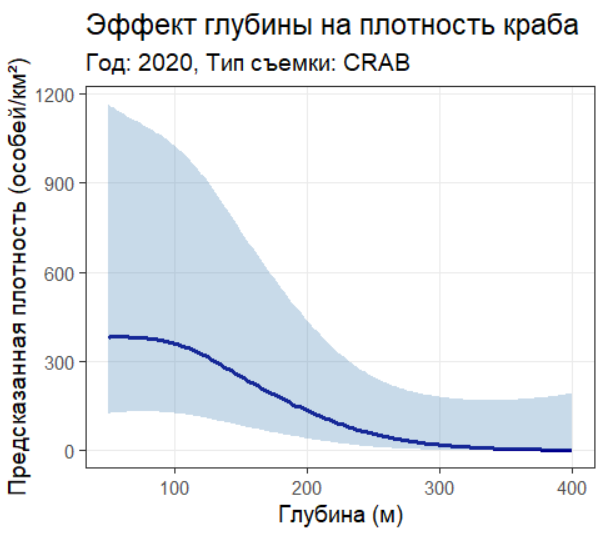
\includegraphics[width=0.6\linewidth,height=\textheight,keepaspectratio]{images/sdmTMB8.PNG}

}

\caption{Рис. 9.: Визуализация эффекта глубины на плотность краба}

\end{figure}%

\section{Карта с акцентом на нулевые
уловы}\label{ux43aux430ux440ux442ux430-ux441-ux430ux43aux446ux435ux43dux442ux43eux43c-ux43dux430-ux43dux443ux43bux435ux432ux44bux435-ux443ux43bux43eux432ux44b}

Повторяем базовую оценку, но меняем в карте нулевые уловы на крестики

\begin{figure}[H]

{\centering 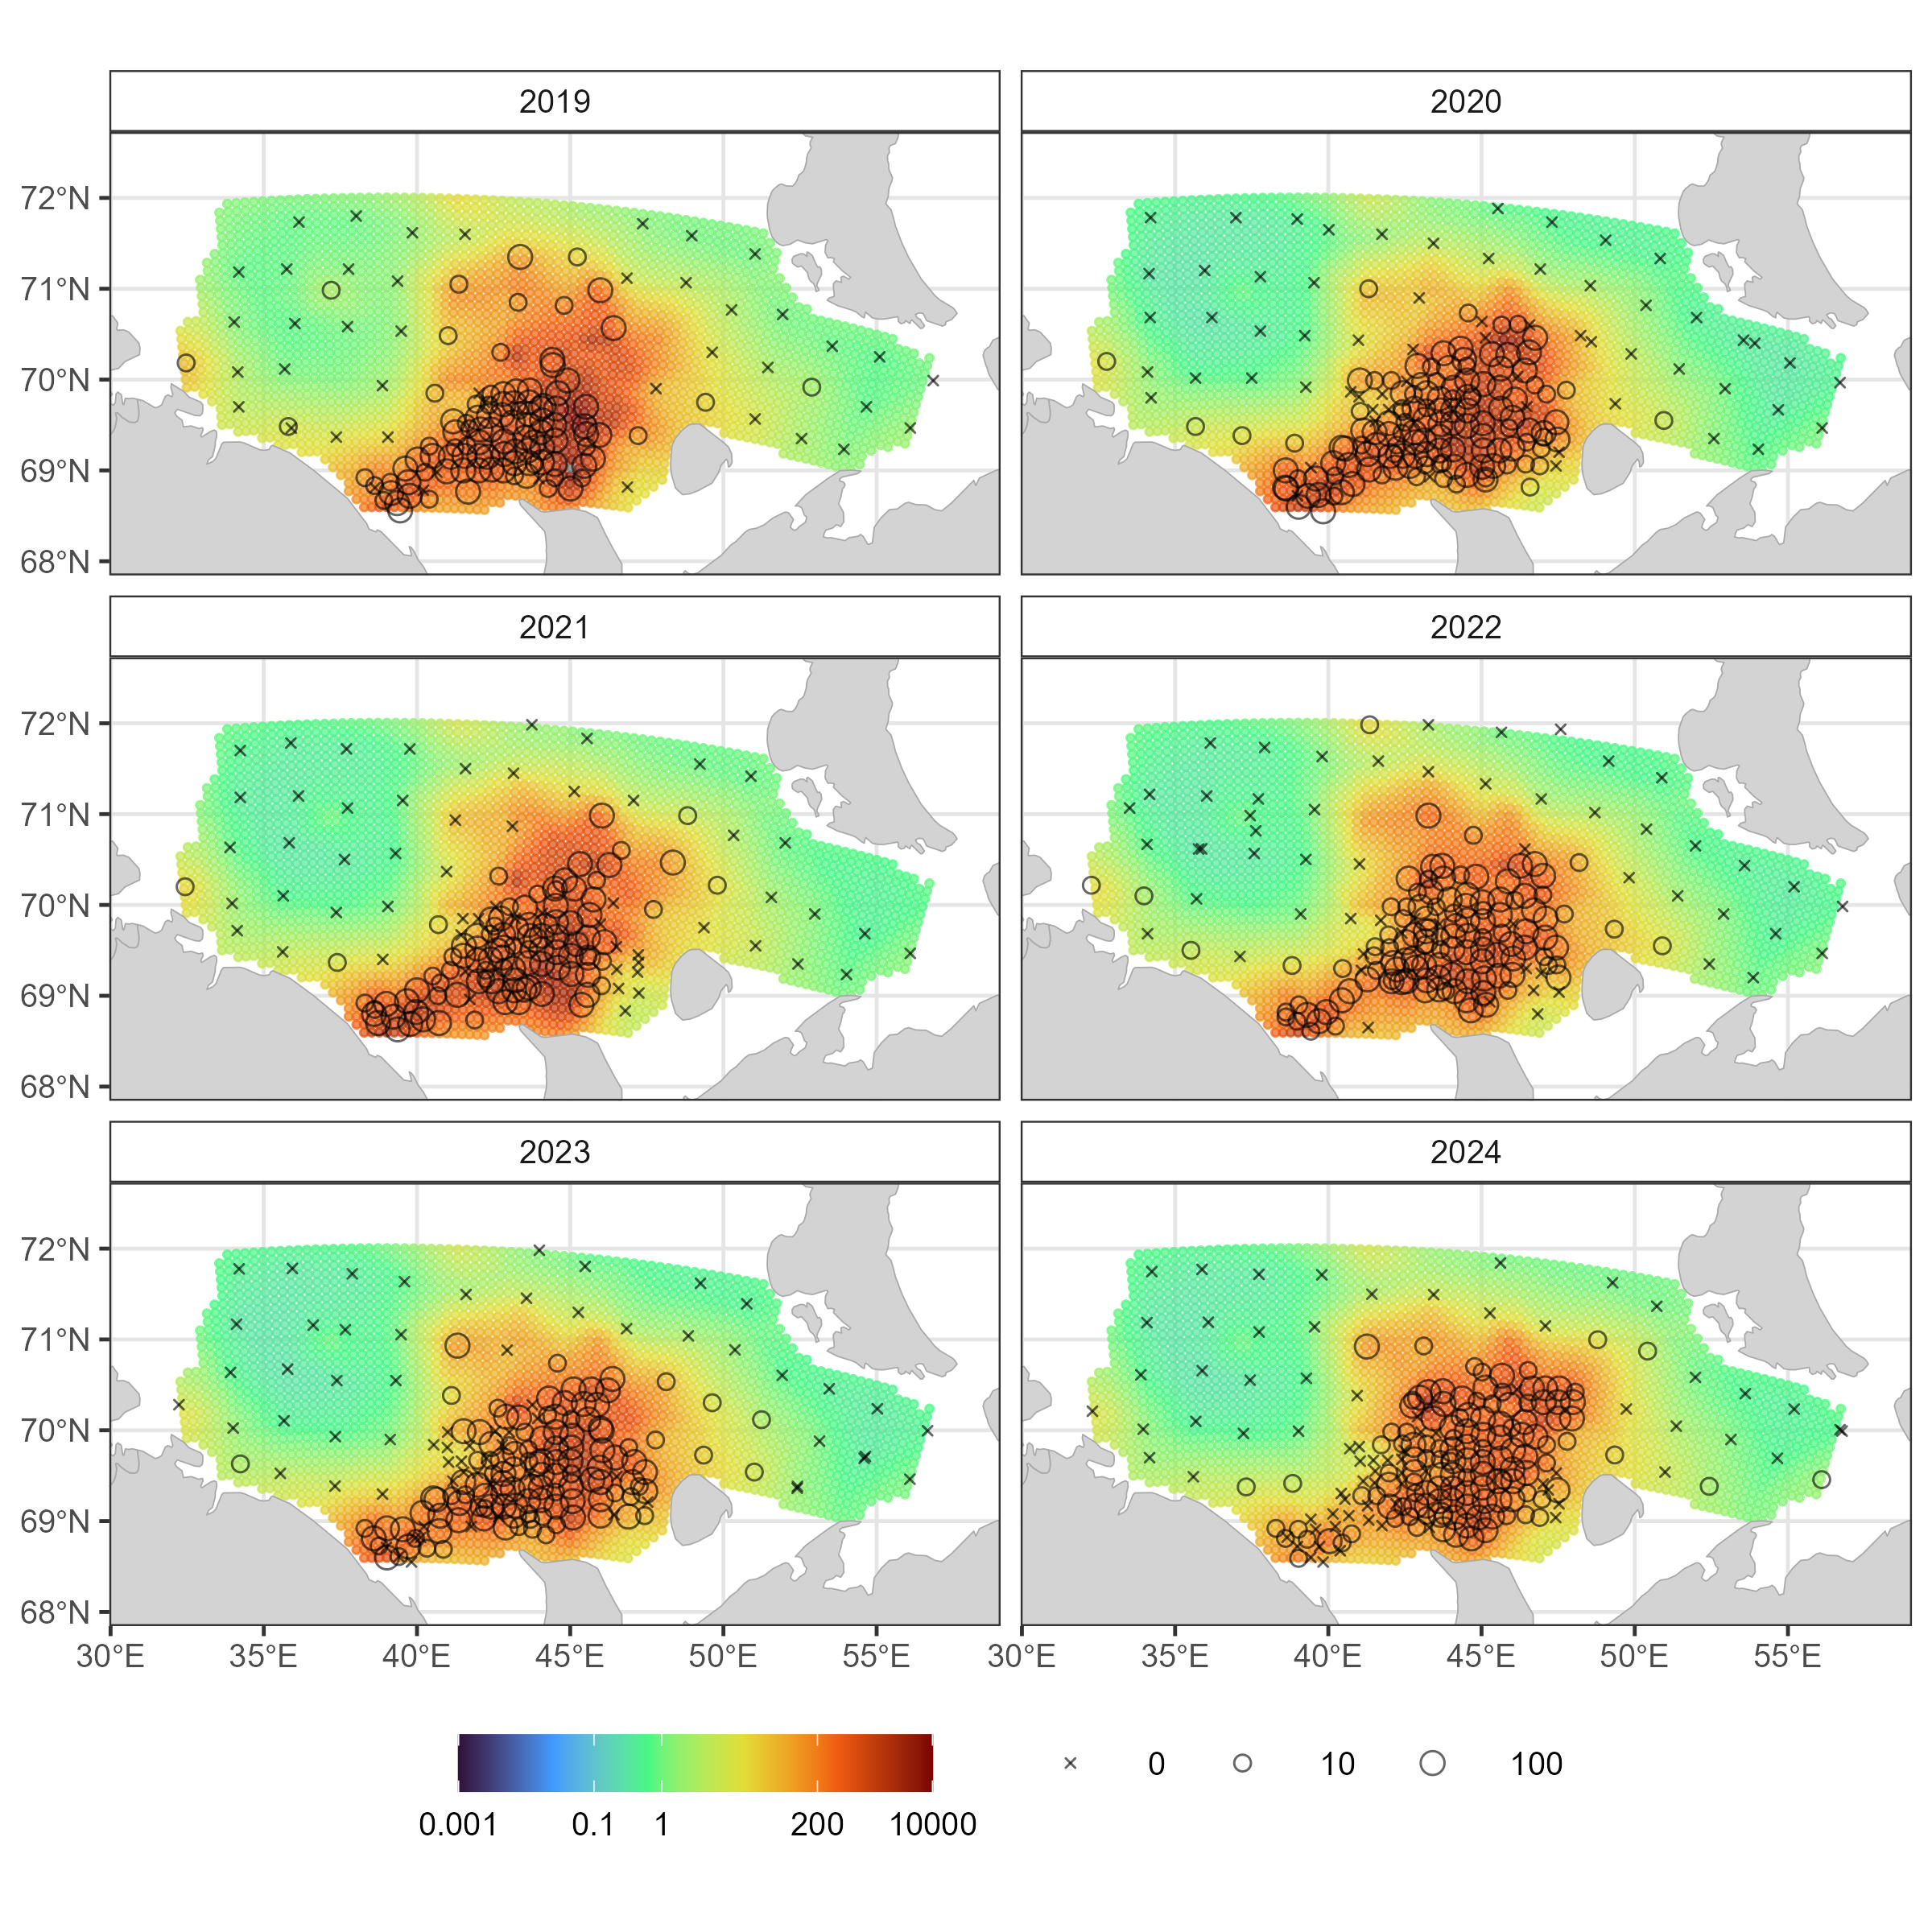
\includegraphics[width=0.9\linewidth,height=\textheight,keepaspectratio]{images/sdmTMBmapZero.jpg}

}

\caption{Рис. 10.: Визуализация результатов (КАРТА)}

\end{figure}%

Скрипт для карты с базовой оценкой

\begin{Shaded}
\begin{Highlighting}[]
\CommentTok{\# {-}{-}{-}{-}{-}{-}{-}{-}{-}{-}{-}{-}{-}{-}{-}{-}{-}{-}{-}{-}{-}{-}{-}{-}{-}{-}{-}}
\CommentTok{\# 1. ПОДГОТОВКА СРЕДЫ И ДАННЫХ}
\CommentTok{\# {-}{-}{-}{-}{-}{-}{-}{-}{-}{-}{-}{-}{-}{-}{-}{-}{-}{-}{-}{-}{-}{-}{-}{-}{-}{-}{-}}

\CommentTok{\# Очистка рабочей среды}
\FunctionTok{rm}\NormalTok{(}\AttributeTok{list =} \FunctionTok{ls}\NormalTok{())}

\CommentTok{\# Установка рабочей директории (замените на свою)}
\FunctionTok{setwd}\NormalTok{(}\StringTok{"C:/COMBINE/"}\NormalTok{)}

\CommentTok{\# Загрузка необходимых пакетов}
\FunctionTok{library}\NormalTok{(readxl)       }\CommentTok{\# Для чтения Excel{-}файлов}
\FunctionTok{library}\NormalTok{(ggplot2)      }\CommentTok{\# Визуализация данных}
\FunctionTok{library}\NormalTok{(dplyr)        }\CommentTok{\# Обработка данных}
\FunctionTok{library}\NormalTok{(PBSmapping)   }\CommentTok{\# Для работы с пространственными данными}
\FunctionTok{library}\NormalTok{(sdmTMB)       }\CommentTok{\# Пространственно{-}временное моделирование}
\FunctionTok{library}\NormalTok{(INLA)         }\CommentTok{\# Продвинутые пространственные модели}
\FunctionTok{library}\NormalTok{(sp)           }\CommentTok{\# Классы для пространственных данных}
\FunctionTok{library}\NormalTok{(sf)           }\CommentTok{\# Пространственные данные (современный формат)}
\FunctionTok{library}\NormalTok{(rnaturalearth) }\CommentTok{\# Загрузка картографических данных}

\CommentTok{\# Загрузка данных из Excel{-}файла}
\NormalTok{data }\OtherTok{\textless{}{-}}\NormalTok{ readxl}\SpecialCharTok{::}\FunctionTok{read\_excel}\NormalTok{(}\StringTok{"KARTOGRAPHIC.xlsx"}\NormalTok{, }\AttributeTok{sheet =} \StringTok{"SURVEY"}\NormalTok{)}

\CommentTok{\# Просмотр структуры данных}
\FunctionTok{str}\NormalTok{(data)}


\CommentTok{\# {-}{-}{-}{-}{-}{-}{-}{-}{-}{-}{-}{-}{-}{-}{-}{-}{-}{-}{-}{-}{-}{-}{-}{-}{-}{-}{-}{-}{-}{-}{-}{-}{-}{-}{-}{-}{-}{-}{-}{-}{-}{-}{-}{-}{-}{-}{-}{-}{-}{-}}
\CommentTok{\# 2. ПРЕОБРАЗОВАНИЕ КООРДИНАТ В ПРОЕКЦИЮ UTM (в км)}
\CommentTok{\# {-}{-}{-}{-}{-}{-}{-}{-}{-}{-}{-}{-}{-}{-}{-}{-}{-}{-}{-}{-}{-}{-}{-}{-}{-}{-}{-}{-}{-}{-}{-}{-}{-}{-}{-}{-}{-}{-}{-}{-}{-}{-}{-}{-}{-}{-}{-}{-}{-}{-}}

\CommentTok{\# Создание пространственного объекта из данных}
\NormalTok{data\_sf }\OtherTok{\textless{}{-}} \FunctionTok{st\_as\_sf}\NormalTok{(}
\NormalTok{  data, }
  \AttributeTok{coords =} \FunctionTok{c}\NormalTok{(}\StringTok{"X"}\NormalTok{, }\StringTok{"Y"}\NormalTok{), }\CommentTok{\# Указание столбцов с координатами}
  \AttributeTok{crs =} \DecValTok{4326}            \CommentTok{\# Система координат WGS84 (широта/долгота)}
\NormalTok{) }

\CommentTok{\# Преобразование в UTM зону 37N (метры)}
\NormalTok{data\_utm }\OtherTok{\textless{}{-}} \FunctionTok{st\_transform}\NormalTok{(data\_sf, }\AttributeTok{crs =} \DecValTok{32637}\NormalTok{) }

\CommentTok{\# Извлечение координат и перевод в километры}
\NormalTok{utm\_coords }\OtherTok{\textless{}{-}} \FunctionTok{st\_coordinates}\NormalTok{(data\_utm)}
\NormalTok{data}\SpecialCharTok{$}\NormalTok{xkm }\OtherTok{\textless{}{-}}\NormalTok{ utm\_coords[, }\DecValTok{1}\NormalTok{] }\SpecialCharTok{/} \DecValTok{1000}  \CommentTok{\# X в км}
\NormalTok{data}\SpecialCharTok{$}\NormalTok{ykm }\OtherTok{\textless{}{-}}\NormalTok{ utm\_coords[, }\DecValTok{2}\NormalTok{] }\SpecialCharTok{/} \DecValTok{1000}  \CommentTok{\# Y в км}

\CommentTok{\# Очистка временных объектов}
\FunctionTok{rm}\NormalTok{(data\_sf, data\_utm, utm\_coords)}

\CommentTok{\# {-}{-}{-}{-}{-}{-}{-}{-}{-}{-}{-}{-}{-}{-}{-}{-}{-}{-}{-}{-}{-}{-}{-}{-}{-}{-}{-}{-}{-}{-}{-}{-}{-}{-}{-}{-}{-}{-}{-}{-}{-}}
\CommentTok{\# 3. ОПРЕДЕЛЕНИЕ ГРАНИЦ ИССЛЕДОВАНИЯ}
\CommentTok{\# {-}{-}{-}{-}{-}{-}{-}{-}{-}{-}{-}{-}{-}{-}{-}{-}{-}{-}{-}{-}{-}{-}{-}{-}{-}{-}{-}{-}{-}{-}{-}{-}{-}{-}{-}{-}{-}{-}{-}{-}{-}}

\CommentTok{\# Вычисление границ исследовательского полигона}
\NormalTok{xl }\OtherTok{\textless{}{-}} \FunctionTok{c}\NormalTok{(}\FunctionTok{min}\NormalTok{(data}\SpecialCharTok{$}\NormalTok{xkm), }\FunctionTok{max}\NormalTok{(data}\SpecialCharTok{$}\NormalTok{xkm))  }\CommentTok{\# Границы по X}
\NormalTok{yl }\OtherTok{\textless{}{-}} \FunctionTok{c}\NormalTok{(}\FunctionTok{min}\NormalTok{(data}\SpecialCharTok{$}\NormalTok{ykm), }\FunctionTok{max}\NormalTok{(data}\SpecialCharTok{$}\NormalTok{ykm))  }\CommentTok{\# Границы по Y}

\CommentTok{\# {-}{-}{-}{-}{-}{-}{-}{-}{-}{-}{-}{-}{-}{-}{-}{-}{-}{-}{-}{-}{-}{-}{-}{-}{-}{-}{-}{-}{-}{-}{-}{-}{-}{-}{-}{-}{-}{-}{-}{-}}
\CommentTok{\# 4. СОЗДАНИЕ РАСТРОВОЙ СЕТКИ ДЛЯ МОДЕЛИ}
\CommentTok{\# {-}{-}{-}{-}{-}{-}{-}{-}{-}{-}{-}{-}{-}{-}{-}{-}{-}{-}{-}{-}{-}{-}{-}{-}{-}{-}{-}{-}{-}{-}{-}{-}{-}{-}{-}{-}{-}{-}{-}{-}}

\CommentTok{\# Создание равномерной сетки с шагом 10 км (для визуализации карты использовался шаг 2 км}
\NormalTok{GRID }\OtherTok{\textless{}{-}} \FunctionTok{makeGrid}\NormalTok{(}
  \AttributeTok{x =} \FunctionTok{seq}\NormalTok{(xl[}\DecValTok{1}\NormalTok{], xl[}\DecValTok{2}\NormalTok{], }\DecValTok{10}\NormalTok{), }
  \AttributeTok{y =} \FunctionTok{seq}\NormalTok{(yl[}\DecValTok{1}\NormalTok{], yl[}\DecValTok{2}\NormalTok{], }\DecValTok{10}\NormalTok{),}
  \AttributeTok{byrow =} \ConstantTok{FALSE}\NormalTok{,}
  \AttributeTok{projection =} \StringTok{"UTM"}\NormalTok{, }
  \AttributeTok{zone =} \DecValTok{37}
\NormalTok{)}

\CommentTok{\# Расчет центроидов ячеек сетки}
\NormalTok{GRID }\OtherTok{\textless{}{-}} \FunctionTok{calcCentroid}\NormalTok{(GRID, }\AttributeTok{rollup =} \DecValTok{3}\NormalTok{)}

\CommentTok{\# {-}{-}{-}{-}{-}{-}{-}{-}{-}{-}{-}{-}{-}{-}{-}{-}{-}{-}{-}{-}{-}{-}{-}{-}{-}{-}{-}{-}{-}{-}{-}{-}{-}{-}{-}{-}{-}{-}{-}{-}{-}{-}{-}{-}{-}{-}{-}{-}{-}{-}{-}{-}{-}{-}{-}{-}{-}{-}{-}}
\CommentTok{\# 5. ПОСТРОЕНИЕ ВЫПУКЛОЙ ОБОЛОЧКИ (CONVEX HULL) ДЛЯ ДАННЫХ}
\CommentTok{\# {-}{-}{-}{-}{-}{-}{-}{-}{-}{-}{-}{-}{-}{-}{-}{-}{-}{-}{-}{-}{-}{-}{-}{-}{-}{-}{-}{-}{-}{-}{-}{-}{-}{-}{-}{-}{-}{-}{-}{-}{-}{-}{-}{-}{-}{-}{-}{-}{-}{-}{-}{-}{-}{-}{-}{-}{-}{-}{-}}

\CommentTok{\# Создание выпуклой оболочки вокруг точек данных}
\NormalTok{Hull }\OtherTok{\textless{}{-}} \FunctionTok{inla.nonconvex.hull}\NormalTok{(}\FunctionTok{cbind}\NormalTok{(data}\SpecialCharTok{$}\NormalTok{xkm, data}\SpecialCharTok{$}\NormalTok{ykm), }\AttributeTok{convex =} \SpecialCharTok{{-}}\FloatTok{0.03}\NormalTok{)}

\CommentTok{\# Визуализация оболочки }
 \FunctionTok{plot}\NormalTok{(Hull)}

\CommentTok{\# Визуализация оболочки и точек съемок 2019{-}2024}
\FunctionTok{points}\NormalTok{(data}\SpecialCharTok{$}\NormalTok{xkm, data}\SpecialCharTok{$}\NormalTok{ykm, }\AttributeTok{pch=}\DecValTok{1}\NormalTok{, }\AttributeTok{cex=}\FloatTok{0.55}\NormalTok{,}\AttributeTok{col=}\StringTok{"black"}\NormalTok{)}


\CommentTok{\# Фильтрация сетки: оставляем только точки внутри оболочки}
\NormalTok{line }\OtherTok{\textless{}{-}}\NormalTok{ Hull}\SpecialCharTok{$}\NormalTok{loc[, }\DecValTok{1}\SpecialCharTok{:}\DecValTok{2}\NormalTok{] }\SpecialCharTok{\%\textgreater{}\%} \FunctionTok{as.data.frame}\NormalTok{()}
\FunctionTok{colnames}\NormalTok{(line) }\OtherTok{\textless{}{-}} \FunctionTok{c}\NormalTok{(}\StringTok{"X"}\NormalTok{, }\StringTok{"Y"}\NormalTok{)}
\NormalTok{GRID}\SpecialCharTok{$}\NormalTok{AREA }\OtherTok{\textless{}{-}} \FunctionTok{point.in.polygon}\NormalTok{(GRID}\SpecialCharTok{$}\NormalTok{X, GRID}\SpecialCharTok{$}\NormalTok{Y, line}\SpecialCharTok{$}\NormalTok{X, line}\SpecialCharTok{$}\NormalTok{Y)}
\NormalTok{GRID }\OtherTok{\textless{}{-}}\NormalTok{ GRID[GRID}\SpecialCharTok{$}\NormalTok{AREA }\SpecialCharTok{\textgreater{}} \FloatTok{0.1}\NormalTok{, }\FunctionTok{c}\NormalTok{(}\StringTok{"X"}\NormalTok{, }\StringTok{"Y"}\NormalTok{)]  }\CommentTok{\# Только внутренние точки}

\CommentTok{\# {-}{-}{-}{-}{-}{-}{-}{-}{-}{-}{-}{-}{-}{-}{-}{-}{-}{-}{-}{-}{-}{-}{-}{-}{-}{-}{-}{-}{-}{-}{-}{-}{-}{-}{-}{-}{-}{-}{-}{-}{-}{-}{-}{-}{-}{-}{-}{-}{-}}
\CommentTok{\# 6. ПОДГОТОВКА СЕТКИ ДЛЯ ПРОГНОЗИРОВАНИЯ}
\CommentTok{\# {-}{-}{-}{-}{-}{-}{-}{-}{-}{-}{-}{-}{-}{-}{-}{-}{-}{-}{-}{-}{-}{-}{-}{-}{-}{-}{-}{-}{-}{-}{-}{-}{-}{-}{-}{-}{-}{-}{-}{-}{-}{-}{-}{-}{-}{-}{-}{-}{-}}

\CommentTok{\# Создание временной сетки (для каждого года)}
\NormalTok{grid }\OtherTok{\textless{}{-}} \FunctionTok{replicate\_df}\NormalTok{(GRID, }\StringTok{"YEAR"}\NormalTok{, }\FunctionTok{unique}\NormalTok{(data}\SpecialCharTok{$}\NormalTok{YEAR))}
\FunctionTok{colnames}\NormalTok{(grid) }\OtherTok{\textless{}{-}} \FunctionTok{c}\NormalTok{(}\StringTok{"xkm"}\NormalTok{, }\StringTok{"ykm"}\NormalTok{, }\StringTok{"YEAR"}\NormalTok{)}
\NormalTok{grid}\SpecialCharTok{$}\NormalTok{SURV }\OtherTok{\textless{}{-}} \StringTok{"CRAB"}  \CommentTok{\# Добавляем информацию о типе съемки}

\CommentTok{\# Визуализация оболочки и сетки для прогнозирования (grid\}}
 \FunctionTok{plot}\NormalTok{(Hull)}
 \FunctionTok{points}\NormalTok{(grid}\SpecialCharTok{$}\NormalTok{xkm, grid}\SpecialCharTok{$}\NormalTok{ykm, }\AttributeTok{pch=}\DecValTok{1}\NormalTok{, }\AttributeTok{cex=}\FloatTok{0.55}\NormalTok{,}\AttributeTok{col=}\StringTok{"black"}\NormalTok{)}

\CommentTok{\# {-}{-}{-}{-}{-}{-}{-}{-}{-}{-}{-}{-}{-}{-}{-}{-}{-}{-}{-}{-}{-}{-}{-}{-}{-}{-}{-}{-}{-}{-}{-}{-}{-}{-}{-}{-}{-}{-}{-}{-}{-}{-}{-}{-}{-}{-}{-}{-}{-}{-}{-}}
\CommentTok{\# 7. ПОСТРОЕНИЕ ПРОСТРАНСТВЕННОЙ СЕТКИ (MESH)}
\CommentTok{\# {-}{-}{-}{-}{-}{-}{-}{-}{-}{-}{-}{-}{-}{-}{-}{-}{-}{-}{-}{-}{-}{-}{-}{-}{-}{-}{-}{-}{-}{-}{-}{-}{-}{-}{-}{-}{-}{-}{-}{-}{-}{-}{-}{-}{-}{-}{-}{-}{-}{-}{-}}

\CommentTok{\# Создание треугольной сетки для пространственного моделирования}
\NormalTok{mesh\_sdm }\OtherTok{\textless{}{-}} \FunctionTok{make\_mesh}\NormalTok{(}
\NormalTok{  data, }
  \FunctionTok{c}\NormalTok{(}\StringTok{"xkm"}\NormalTok{, }\StringTok{"ykm"}\NormalTok{),  }\CommentTok{\# Координаты}
  \AttributeTok{cutoff =} \DecValTok{10}        \CommentTok{\# Минимальное расстояние между узлами (км)}
\NormalTok{)}

\CommentTok{\# Визуализация сетки (раскомментируйте)}
 \FunctionTok{plot}\NormalTok{(mesh\_sdm)}

\CommentTok{\# {-}{-}{-}{-}{-}{-}{-}{-}{-}{-}{-}{-}{-}{-}{-}{-}{-}{-}{-}{-}{-}{-}{-}{-}{-}{-}{-}{-}{-}{-}{-}{-}{-}{-}{-}{-}{-}{-}{-}{-}{-}{-}{-}{-}{-}{-}{-}{-}{-}{-}{-}}
\CommentTok{\# 8. ПОСТРОЕНИЕ ПРОСТРАНСТВЕННО{-}ВРЕМЕННОЙ МОДЕЛИ}
\CommentTok{\# {-}{-}{-}{-}{-}{-}{-}{-}{-}{-}{-}{-}{-}{-}{-}{-}{-}{-}{-}{-}{-}{-}{-}{-}{-}{-}{-}{-}{-}{-}{-}{-}{-}{-}{-}{-}{-}{-}{-}{-}{-}{-}{-}{-}{-}{-}{-}{-}{-}{-}{-}}

\NormalTok{m }\OtherTok{\textless{}{-}} \FunctionTok{sdmTMB}\NormalTok{(}
  \AttributeTok{data =}\NormalTok{ data, }
  \AttributeTok{formula =}\NormalTok{ Density }\SpecialCharTok{\textasciitilde{}} \DecValTok{0} \SpecialCharTok{+} \FunctionTok{as.factor}\NormalTok{(YEAR),  }\CommentTok{\# Формула: плотность зависит от года}
  \AttributeTok{time =} \StringTok{"YEAR"}\NormalTok{,         }\CommentTok{\# Временная переменная}
  \AttributeTok{mesh =}\NormalTok{ mesh\_sdm,       }\CommentTok{\# Пространственная сетка}
  \AttributeTok{family =} \FunctionTok{tweedie}\NormalTok{(}\AttributeTok{link =} \StringTok{"log"}\NormalTok{),  }\CommentTok{\# Статистическое распределение}
  \AttributeTok{spatial =} \StringTok{"on"}\NormalTok{,        }\CommentTok{\# Включение пространственных эффектов}
  \AttributeTok{spatiotemporal =} \StringTok{"iid"} \CommentTok{\# Пространственно{-}временные эффекты}
\NormalTok{)}


\CommentTok{\# Вывод результатов модели}
\FunctionTok{summary}\NormalTok{(m)}
\FunctionTok{AIC}\NormalTok{(m)  }\CommentTok{\# Критерий Акаике}
\FunctionTok{sanity}\NormalTok{(m)  }\CommentTok{\# Проверка корректности модели}

\CommentTok{\# {-}{-}{-}{-}{-}{-}{-}{-}{-}{-}{-}{-}{-}{-}{-}{-}{-}{-}{-}{-}{-}{-}{-}{-}{-}{-}{-}{-}{-}{-}{-}{-}{-}{-}{-}{-}{-}{-}{-}{-}{-}{-}{-}{-}{-}{-}{-}{-}{-}{-}{-}}
\CommentTok{\# 9. ДИАГНОСТИКА МОДЕЛИ}
\CommentTok{\# {-}{-}{-}{-}{-}{-}{-}{-}{-}{-}{-}{-}{-}{-}{-}{-}{-}{-}{-}{-}{-}{-}{-}{-}{-}{-}{-}{-}{-}{-}{-}{-}{-}{-}{-}{-}{-}{-}{-}{-}{-}{-}{-}{-}{-}{-}{-}{-}{-}{-}{-}}

\CommentTok{\# Расчет остатков модели}
\NormalTok{data}\SpecialCharTok{$}\NormalTok{resids }\OtherTok{\textless{}{-}} \FunctionTok{residuals}\NormalTok{(m) }

\CommentTok{\# Гистограмма остатков}
\FunctionTok{hist}\NormalTok{(data}\SpecialCharTok{$}\NormalTok{resids)}

\CommentTok{\# График квантиль{-}квантиль}
\FunctionTok{qqnorm}\NormalTok{(data}\SpecialCharTok{$}\NormalTok{resids)}
\FunctionTok{abline}\NormalTok{(}\AttributeTok{a =} \DecValTok{0}\NormalTok{, }\AttributeTok{b =} \DecValTok{1}\NormalTok{)}

\CommentTok{\# {-}{-}{-}{-}{-}{-}{-}{-}{-}{-}{-}{-}{-}{-}{-}{-}{-}{-}{-}{-}{-}{-}{-}{-}{-}{-}{-}{-}{-}{-}{-}{-}{-}{-}{-}{-}{-}{-}{-}{-}{-}{-}{-}{-}{-}{-}{-}{-}{-}{-}{-}}
\CommentTok{\# 10. ПРОГНОЗИРОВАНИЕ НА СЕТКЕ}
\CommentTok{\# {-}{-}{-}{-}{-}{-}{-}{-}{-}{-}{-}{-}{-}{-}{-}{-}{-}{-}{-}{-}{-}{-}{-}{-}{-}{-}{-}{-}{-}{-}{-}{-}{-}{-}{-}{-}{-}{-}{-}{-}{-}{-}{-}{-}{-}{-}{-}{-}{-}{-}{-}}

\CommentTok{\# Прогноз значений плотности на сетке}
\NormalTok{predictions }\OtherTok{\textless{}{-}} \FunctionTok{predict}\NormalTok{(m, }\AttributeTok{newdata =}\NormalTok{ grid, }\AttributeTok{return\_tmb\_object =} \ConstantTok{TRUE}\NormalTok{)}
\NormalTok{RASP }\OtherTok{\textless{}{-}}\NormalTok{ predictions}\SpecialCharTok{$}\NormalTok{data}

\CommentTok{\# Преобразование координат обратно в широту/долготу}
\NormalTok{RASP}\SpecialCharTok{$}\NormalTok{xkm\_m }\OtherTok{\textless{}{-}}\NormalTok{ RASP}\SpecialCharTok{$}\NormalTok{xkm }\SpecialCharTok{*} \DecValTok{1000}  \CommentTok{\# Обратно в метры}
\NormalTok{RASP}\SpecialCharTok{$}\NormalTok{ykm\_m }\OtherTok{\textless{}{-}}\NormalTok{ RASP}\SpecialCharTok{$}\NormalTok{ykm }\SpecialCharTok{*} \DecValTok{1000}

\CommentTok{\# Создание пространственного объекта в UTM}
\NormalTok{utm\_proj }\OtherTok{\textless{}{-}} \FunctionTok{CRS}\NormalTok{(}\StringTok{"+proj=utm +zone=37 +datum=WGS84 +units=m +no\_defs"}\NormalTok{)}
\NormalTok{coords }\OtherTok{\textless{}{-}} \FunctionTok{cbind}\NormalTok{(RASP}\SpecialCharTok{$}\NormalTok{xkm\_m, RASP}\SpecialCharTok{$}\NormalTok{ykm\_m)}
\NormalTok{sp\_points }\OtherTok{\textless{}{-}} \FunctionTok{SpatialPoints}\NormalTok{(coords, }\AttributeTok{proj4string =}\NormalTok{ utm\_proj)}

\CommentTok{\# Преобразование в WGS84 (широта/долгота)}
\NormalTok{wgs84\_proj }\OtherTok{\textless{}{-}} \FunctionTok{CRS}\NormalTok{(}\StringTok{"+proj=longlat +datum=WGS84"}\NormalTok{)}
\NormalTok{sp\_points\_latlon }\OtherTok{\textless{}{-}} \FunctionTok{spTransform}\NormalTok{(sp\_points, wgs84\_proj)}

\CommentTok{\# Добавление координат в основной датафрейм}
\NormalTok{RASP}\SpecialCharTok{$}\NormalTok{X }\OtherTok{\textless{}{-}} \FunctionTok{coordinates}\NormalTok{(sp\_points\_latlon)[, }\DecValTok{1}\NormalTok{]  }\CommentTok{\# Долгота}
\NormalTok{RASP}\SpecialCharTok{$}\NormalTok{Y }\OtherTok{\textless{}{-}} \FunctionTok{coordinates}\NormalTok{(sp\_points\_latlon)[, }\DecValTok{2}\NormalTok{]  }\CommentTok{\# Широта}

\CommentTok{\# Удаление временных столбцов}
\NormalTok{RASP}\SpecialCharTok{$}\NormalTok{xkm\_m }\OtherTok{\textless{}{-}} \ConstantTok{NULL}
\NormalTok{RASP}\SpecialCharTok{$}\NormalTok{ykm\_m }\OtherTok{\textless{}{-}} \ConstantTok{NULL}

\CommentTok{\# Проверка структуры результата}
\FunctionTok{str}\NormalTok{(RASP)}

\CommentTok{\# {-}{-}{-}{-}{-}{-}{-}{-}{-}{-}{-}{-}{-}{-}{-}{-}{-}{-}{-}{-}{-}{-}{-}{-}{-}{-}{-}{-}{-}{-}{-}{-}{-}{-}{-}{-}{-}{-}{-}{-}{-}{-}{-}{-}{-}}
\CommentTok{\# 11. ВИЗУАЛИЗАЦИЯ РЕЗУЛЬТАТОВ (КАРТА)}
\CommentTok{\# {-}{-}{-}{-}{-}{-}{-}{-}{-}{-}{-}{-}{-}{-}{-}{-}{-}{-}{-}{-}{-}{-}{-}{-}{-}{-}{-}{-}{-}{-}{-}{-}{-}{-}{-}{-}{-}{-}{-}{-}{-}{-}{-}{-}{-}}

\CommentTok{\# Загрузка картографических данных}
\NormalTok{world }\OtherTok{\textless{}{-}} \FunctionTok{ne\_countries}\NormalTok{(}\AttributeTok{scale =} \StringTok{"medium"}\NormalTok{, }\AttributeTok{returnclass =} \StringTok{"sf"}\NormalTok{)}

\CommentTok{\# Определение региона интереса (Арктика России)}
\NormalTok{arctic\_bbox }\OtherTok{\textless{}{-}} \FunctionTok{st\_bbox}\NormalTok{(}\FunctionTok{c}\NormalTok{(}\AttributeTok{xmin =} \DecValTok{25}\NormalTok{, }\AttributeTok{xmax =} \DecValTok{70}\NormalTok{, }\AttributeTok{ymin =} \DecValTok{65}\NormalTok{, }\AttributeTok{ymax =} \DecValTok{80}\NormalTok{), }\AttributeTok{crs =} \DecValTok{4326}\NormalTok{)}
\NormalTok{arctic }\OtherTok{\textless{}{-}} \FunctionTok{st\_crop}\NormalTok{(world, arctic\_bbox)}

\CommentTok{\# Определяем кастомные breaks для шкалы}
\NormalTok{my\_breaks }\OtherTok{\textless{}{-}} \FunctionTok{c}\NormalTok{(}\FloatTok{0.001}\NormalTok{,}\FloatTok{0.1}\NormalTok{,}\DecValTok{1}\NormalTok{,  }\DecValTok{200}\NormalTok{, }\DecValTok{10000}\NormalTok{)}

\CommentTok{\# Создаем категории для PROM}
\NormalTok{data }\OtherTok{\textless{}{-}}\NormalTok{ data }\SpecialCharTok{\%\textgreater{}\%}
  \FunctionTok{mutate}\NormalTok{(}
    \AttributeTok{PROM\_cat =} \FunctionTok{case\_when}\NormalTok{(}
\NormalTok{      PROM }\SpecialCharTok{==} \DecValTok{0} \SpecialCharTok{\textasciitilde{}} \StringTok{"0"}\NormalTok{,}
\NormalTok{      PROM }\SpecialCharTok{\textgreater{}=} \DecValTok{1} \SpecialCharTok{\&}\NormalTok{ PROM }\SpecialCharTok{\textless{}} \DecValTok{10} \SpecialCharTok{\textasciitilde{}} \StringTok{"1{-}9"}\NormalTok{,}
\NormalTok{      PROM }\SpecialCharTok{\textgreater{}=} \DecValTok{10} \SpecialCharTok{\&}\NormalTok{ PROM }\SpecialCharTok{\textless{}} \DecValTok{100} \SpecialCharTok{\textasciitilde{}} \StringTok{"10{-}99"}\NormalTok{,}
\NormalTok{      PROM }\SpecialCharTok{\textgreater{}=} \DecValTok{100} \SpecialCharTok{\textasciitilde{}} \StringTok{"100+"}
\NormalTok{    ),}
    \AttributeTok{PROM\_cat =} \FunctionTok{factor}\NormalTok{(PROM\_cat, }\AttributeTok{levels =} \FunctionTok{c}\NormalTok{(}\StringTok{"0"}\NormalTok{, }\StringTok{"1{-}9"}\NormalTok{, }\StringTok{"10{-}99"}\NormalTok{, }\StringTok{"100+"}\NormalTok{)),}
    \AttributeTok{shape\_cat =} \FunctionTok{ifelse}\NormalTok{(PROM\_cat }\SpecialCharTok{==} \StringTok{"0"}\NormalTok{, }\StringTok{"zero"}\NormalTok{, }\StringTok{"non\_zero"}\NormalTok{)}
\NormalTok{  )}

\CommentTok{\# Обновляем график}
\FunctionTok{ggplot}\NormalTok{() }\SpecialCharTok{+}
  \FunctionTok{geom\_point}\NormalTok{(}
    \AttributeTok{data =}\NormalTok{ RASP, }
    \FunctionTok{aes}\NormalTok{(}\AttributeTok{x =}\NormalTok{ X, }\AttributeTok{y =}\NormalTok{ Y, }\AttributeTok{color =} \FunctionTok{exp}\NormalTok{(est)), }
    \AttributeTok{size =} \FloatTok{0.8}\NormalTok{, }
    \AttributeTok{alpha =} \FloatTok{0.7}
\NormalTok{  ) }\SpecialCharTok{+} 
  \FunctionTok{geom\_point}\NormalTok{(}
    \AttributeTok{data =}\NormalTok{ data, }
    \FunctionTok{aes}\NormalTok{(}\AttributeTok{x =}\NormalTok{ X, }\AttributeTok{y =}\NormalTok{ Y, }\AttributeTok{size =}\NormalTok{ PROM\_cat, }\AttributeTok{shape =}\NormalTok{ shape\_cat),}
    \AttributeTok{color =} \StringTok{"black"}\NormalTok{, }
    \AttributeTok{fill =} \ConstantTok{NA}\NormalTok{, }
    \AttributeTok{alpha =} \FloatTok{0.6}
\NormalTok{  ) }\SpecialCharTok{+}
  \FunctionTok{scale\_size\_manual}\NormalTok{(}
    \AttributeTok{name =} \ConstantTok{NULL}\NormalTok{,}
    \AttributeTok{values =} \FunctionTok{c}\NormalTok{(}\StringTok{"0"} \OtherTok{=} \DecValTok{1}\NormalTok{, }\StringTok{"1{-}9"} \OtherTok{=} \DecValTok{2}\NormalTok{, }\StringTok{"10{-}99"} \OtherTok{=} \DecValTok{3}\NormalTok{),}
    \AttributeTok{labels =} \FunctionTok{c}\NormalTok{(}\StringTok{"0"}\NormalTok{, }\StringTok{"10"}\NormalTok{, }\StringTok{"100"}\NormalTok{)}
\NormalTok{  ) }\SpecialCharTok{+}
  \FunctionTok{scale\_shape\_manual}\NormalTok{(}
    \AttributeTok{values =} \FunctionTok{c}\NormalTok{(}\StringTok{"zero"} \OtherTok{=} \DecValTok{4}\NormalTok{, }\StringTok{"non\_zero"} \OtherTok{=} \DecValTok{21}\NormalTok{),}
    \AttributeTok{guide =} \StringTok{"none"} \CommentTok{\# Скрываем легенду для формы}
\NormalTok{  ) }\SpecialCharTok{+}
  \FunctionTok{guides}\NormalTok{(}
    \AttributeTok{size =} \FunctionTok{guide\_legend}\NormalTok{(}
      \AttributeTok{override.aes =} \FunctionTok{list}\NormalTok{(}\AttributeTok{shape =} \FunctionTok{c}\NormalTok{(}\DecValTok{4}\NormalTok{, }\DecValTok{21}\NormalTok{, }\DecValTok{21}\NormalTok{)) }\CommentTok{\# Крестик только для первого элемента}
\NormalTok{    )}
\NormalTok{  ) }\SpecialCharTok{+}
  \FunctionTok{geom\_sf}\NormalTok{(}\AttributeTok{data =}\NormalTok{ arctic, }\AttributeTok{fill =} \StringTok{"lightgrey"}\NormalTok{, }\AttributeTok{color =} \StringTok{"darkgrey"}\NormalTok{) }\SpecialCharTok{+}
  \FunctionTok{scale\_color\_viridis\_c}\NormalTok{(}
    \AttributeTok{name =} \ConstantTok{NULL}\NormalTok{,}
    \AttributeTok{option =} \StringTok{"H"}\NormalTok{, }
    \AttributeTok{trans =} \StringTok{"log"}\NormalTok{, }
    \AttributeTok{breaks =}\NormalTok{ my\_breaks, }
    \AttributeTok{labels =}\NormalTok{ my\_breaks, }
    \AttributeTok{limits =} \FunctionTok{range}\NormalTok{(my\_breaks),}
    \AttributeTok{guide =} \FunctionTok{guide\_colorbar}\NormalTok{(}
      \AttributeTok{barwidth =} \FunctionTok{unit}\NormalTok{(}\DecValTok{5}\NormalTok{, }\StringTok{"cm"}\NormalTok{),}
      \AttributeTok{title.position =} \StringTok{"top"}\NormalTok{,}
      \AttributeTok{direction =} \StringTok{"horizontal"}
\NormalTok{    )}
\NormalTok{  ) }\SpecialCharTok{+}
  \FunctionTok{facet\_wrap}\NormalTok{(}\SpecialCharTok{\textasciitilde{}}\NormalTok{ YEAR, }\AttributeTok{ncol =} \DecValTok{2}\NormalTok{) }\SpecialCharTok{+}
  \FunctionTok{coord\_sf}\NormalTok{(}
    \AttributeTok{xlim =} \FunctionTok{c}\NormalTok{(}\FunctionTok{min}\NormalTok{(RASP}\SpecialCharTok{$}\NormalTok{X)}\SpecialCharTok{{-}}\DecValTok{1}\NormalTok{, }\FunctionTok{max}\NormalTok{(RASP}\SpecialCharTok{$}\NormalTok{X)}\SpecialCharTok{+}\DecValTok{1}\NormalTok{),}
    \AttributeTok{ylim =} \FunctionTok{c}\NormalTok{(}\FunctionTok{min}\NormalTok{(RASP}\SpecialCharTok{$}\NormalTok{Y)}\SpecialCharTok{{-}}\FloatTok{0.5}\NormalTok{, }\FunctionTok{max}\NormalTok{(RASP}\SpecialCharTok{$}\NormalTok{Y)}\SpecialCharTok{+}\FloatTok{0.5}\NormalTok{),}
    \AttributeTok{crs =} \DecValTok{4326}
\NormalTok{  ) }\SpecialCharTok{+}
  \FunctionTok{theme\_bw}\NormalTok{(}\AttributeTok{base\_size =} \DecValTok{12}\NormalTok{) }\SpecialCharTok{+}
  \FunctionTok{labs}\NormalTok{(}\AttributeTok{x =} \ConstantTok{NULL}\NormalTok{, }\AttributeTok{y =} \ConstantTok{NULL}\NormalTok{) }\SpecialCharTok{+}
  \FunctionTok{theme}\NormalTok{(}
    \AttributeTok{panel.grid =} \FunctionTok{element\_line}\NormalTok{(}\AttributeTok{color =} \StringTok{"grey90"}\NormalTok{),}
    \AttributeTok{legend.position =} \StringTok{"bottom"}\NormalTok{,}
    \AttributeTok{legend.key.width =} \FunctionTok{unit}\NormalTok{(}\FloatTok{1.2}\NormalTok{, }\StringTok{"cm"}\NormalTok{),}
    \AttributeTok{strip.background =} \FunctionTok{element\_rect}\NormalTok{(}\AttributeTok{fill =} \StringTok{"white"}\NormalTok{)}
\NormalTok{  )}


\CommentTok{\# Сохранение графика (раскомментируйте)}
\CommentTok{\# ggsave("sdmTMBmapZero.jpg", width = 8, height = 8, dpi = 300)}
\end{Highlighting}
\end{Shaded}

\section{Определение площади
съемки}\label{ux43eux43fux440ux435ux434ux435ux43bux435ux43dux438ux435-ux43fux43bux43eux449ux430ux434ux438-ux441ux44aux435ux43cux43aux438}

\begin{Shaded}
\begin{Highlighting}[]
\CommentTok{\# {-}{-}{-}{-}{-}{-}{-}{-}{-}{-}{-}{-}{-}{-}{-}{-}{-}{-}{-}{-}{-}{-}{-}{-}{-}{-}{-}}
\CommentTok{\# 1. ПОДГОТОВКА СРЕДЫ И ДАННЫХ}
\CommentTok{\# {-}{-}{-}{-}{-}{-}{-}{-}{-}{-}{-}{-}{-}{-}{-}{-}{-}{-}{-}{-}{-}{-}{-}{-}{-}{-}{-}}

\CommentTok{\# Очистка рабочей среды}
\FunctionTok{rm}\NormalTok{(}\AttributeTok{list =} \FunctionTok{ls}\NormalTok{())}

\CommentTok{\# Установка рабочей директории (замените на свою)}
\FunctionTok{setwd}\NormalTok{(}\StringTok{"C:/COMBINE/"}\NormalTok{)}

\CommentTok{\# Загрузка необходимых пакетов}
\FunctionTok{library}\NormalTok{(readxl)       }\CommentTok{\# Для чтения Excel{-}файлов}
\FunctionTok{library}\NormalTok{(PBSmapping)   }\CommentTok{\# Для работы с пространственными данными}
\FunctionTok{library}\NormalTok{(sdmTMB)       }\CommentTok{\# Пространственно{-}временное моделирование}
\FunctionTok{library}\NormalTok{(INLA)         }\CommentTok{\# Продвинутые пространственные модели}

\CommentTok{\# Загрузка данных из Excel{-}файла}
\NormalTok{data }\OtherTok{\textless{}{-}}\NormalTok{ readxl}\SpecialCharTok{::}\FunctionTok{read\_excel}\NormalTok{(}\StringTok{"KARTOGRAPHIC.xlsx"}\NormalTok{, }\AttributeTok{sheet =} \StringTok{"SURVEY"}\NormalTok{)}

\CommentTok{\# Просмотр структуры данных}
\FunctionTok{str}\NormalTok{(data)}


\CommentTok{\# {-}{-}{-}{-}{-}{-}{-}{-}{-}{-}{-}{-}{-}{-}{-}{-}{-}{-}{-}{-}{-}{-}{-}{-}{-}{-}{-}{-}{-}{-}{-}{-}{-}{-}{-}{-}{-}{-}{-}{-}{-}{-}{-}{-}{-}{-}{-}{-}{-}{-}}
\CommentTok{\# 2. ПРЕОБРАЗОВАНИЕ КООРДИНАТ В ПРОЕКЦИЮ UTM (в км)}
\CommentTok{\# {-}{-}{-}{-}{-}{-}{-}{-}{-}{-}{-}{-}{-}{-}{-}{-}{-}{-}{-}{-}{-}{-}{-}{-}{-}{-}{-}{-}{-}{-}{-}{-}{-}{-}{-}{-}{-}{-}{-}{-}{-}{-}{-}{-}{-}{-}{-}{-}{-}{-}}

\CommentTok{\# Создание пространственного объекта из данных}
\NormalTok{data\_sf }\OtherTok{\textless{}{-}} \FunctionTok{st\_as\_sf}\NormalTok{(}
\NormalTok{  data, }
  \AttributeTok{coords =} \FunctionTok{c}\NormalTok{(}\StringTok{"X"}\NormalTok{, }\StringTok{"Y"}\NormalTok{), }\CommentTok{\# Указание столбцов с координатами}
  \AttributeTok{crs =} \DecValTok{4326}            \CommentTok{\# Система координат WGS84 (широта/долгота)}
\NormalTok{) }

\CommentTok{\# Преобразование в UTM зону 37N (метры)}
\NormalTok{data\_utm }\OtherTok{\textless{}{-}} \FunctionTok{st\_transform}\NormalTok{(data\_sf, }\AttributeTok{crs =} \DecValTok{32637}\NormalTok{) }

\CommentTok{\# Извлечение координат и перевод в километры}
\NormalTok{utm\_coords }\OtherTok{\textless{}{-}} \FunctionTok{st\_coordinates}\NormalTok{(data\_utm)}
\NormalTok{data}\SpecialCharTok{$}\NormalTok{xkm }\OtherTok{\textless{}{-}}\NormalTok{ utm\_coords[, }\DecValTok{1}\NormalTok{] }\SpecialCharTok{/} \DecValTok{1000}  \CommentTok{\# X в км}
\NormalTok{data}\SpecialCharTok{$}\NormalTok{ykm }\OtherTok{\textless{}{-}}\NormalTok{ utm\_coords[, }\DecValTok{2}\NormalTok{] }\SpecialCharTok{/} \DecValTok{1000}  \CommentTok{\# Y в км}

\CommentTok{\# Очистка временных объектов}
\FunctionTok{rm}\NormalTok{(data\_sf, data\_utm, utm\_coords)}

\CommentTok{\# {-}{-}{-}{-}{-}{-}{-}{-}{-}{-}{-}{-}{-}{-}{-}{-}{-}{-}{-}{-}{-}{-}{-}{-}{-}{-}{-}{-}{-}{-}{-}{-}{-}{-}{-}{-}{-}{-}{-}{-}{-}}
\CommentTok{\# 3. ОПРЕДЕЛЕНИЕ ГРАНИЦ ИССЛЕДОВАНИЯ}
\CommentTok{\# {-}{-}{-}{-}{-}{-}{-}{-}{-}{-}{-}{-}{-}{-}{-}{-}{-}{-}{-}{-}{-}{-}{-}{-}{-}{-}{-}{-}{-}{-}{-}{-}{-}{-}{-}{-}{-}{-}{-}{-}{-}}

\CommentTok{\# Вычисление границ исследовательского полигона}
\NormalTok{xl }\OtherTok{\textless{}{-}} \FunctionTok{c}\NormalTok{(}\FunctionTok{min}\NormalTok{(data}\SpecialCharTok{$}\NormalTok{xkm), }\FunctionTok{max}\NormalTok{(data}\SpecialCharTok{$}\NormalTok{xkm))  }\CommentTok{\# Границы по X}
\NormalTok{yl }\OtherTok{\textless{}{-}} \FunctionTok{c}\NormalTok{(}\FunctionTok{min}\NormalTok{(data}\SpecialCharTok{$}\NormalTok{ykm), }\FunctionTok{max}\NormalTok{(data}\SpecialCharTok{$}\NormalTok{ykm))  }\CommentTok{\# Границы по Y}

\CommentTok{\# {-}{-}{-}{-}{-}{-}{-}{-}{-}{-}{-}{-}{-}{-}{-}{-}{-}{-}{-}{-}{-}{-}{-}{-}{-}{-}{-}{-}{-}{-}{-}{-}{-}{-}{-}{-}{-}{-}{-}{-}}
\CommentTok{\# 4. СОЗДАНИЕ РАСТРОВОЙ СЕТКИ ДЛЯ МОДЕЛИ}
\CommentTok{\# {-}{-}{-}{-}{-}{-}{-}{-}{-}{-}{-}{-}{-}{-}{-}{-}{-}{-}{-}{-}{-}{-}{-}{-}{-}{-}{-}{-}{-}{-}{-}{-}{-}{-}{-}{-}{-}{-}{-}{-}}

\CommentTok{\# Создание равномерной сетки с шагом 10 км (для визуализации карты использовался шаг 2 км}
\NormalTok{GRID }\OtherTok{\textless{}{-}} \FunctionTok{makeGrid}\NormalTok{(}
  \AttributeTok{x =} \FunctionTok{seq}\NormalTok{(xl[}\DecValTok{1}\NormalTok{], xl[}\DecValTok{2}\NormalTok{], }\DecValTok{10}\NormalTok{), }
  \AttributeTok{y =} \FunctionTok{seq}\NormalTok{(yl[}\DecValTok{1}\NormalTok{], yl[}\DecValTok{2}\NormalTok{], }\DecValTok{10}\NormalTok{),}
  \AttributeTok{byrow =} \ConstantTok{FALSE}\NormalTok{,}
  \AttributeTok{projection =} \StringTok{"UTM"}\NormalTok{, }
  \AttributeTok{zone =} \DecValTok{37}
\NormalTok{)}

\CommentTok{\# Расчет центроидов ячеек сетки}
\NormalTok{GRID }\OtherTok{\textless{}{-}} \FunctionTok{calcCentroid}\NormalTok{(GRID, }\AttributeTok{rollup =} \DecValTok{3}\NormalTok{)}

\CommentTok{\# {-}{-}{-}{-}{-}{-}{-}{-}{-}{-}{-}{-}{-}{-}{-}{-}{-}{-}{-}{-}{-}{-}{-}{-}{-}{-}{-}{-}{-}{-}{-}{-}{-}{-}{-}{-}{-}{-}{-}{-}{-}{-}{-}{-}{-}{-}{-}{-}{-}{-}{-}{-}{-}{-}{-}{-}{-}{-}{-}}
\CommentTok{\# 5. ПОСТРОЕНИЕ ВЫПУКЛОЙ ОБОЛОЧКИ (CONVEX HULL) ДЛЯ ДАННЫХ}
\CommentTok{\# {-}{-}{-}{-}{-}{-}{-}{-}{-}{-}{-}{-}{-}{-}{-}{-}{-}{-}{-}{-}{-}{-}{-}{-}{-}{-}{-}{-}{-}{-}{-}{-}{-}{-}{-}{-}{-}{-}{-}{-}{-}{-}{-}{-}{-}{-}{-}{-}{-}{-}{-}{-}{-}{-}{-}{-}{-}{-}{-}}

\CommentTok{\# Создание выпуклой оболочки вокруг точек данных}
\NormalTok{Hull }\OtherTok{\textless{}{-}} \FunctionTok{inla.nonconvex.hull}\NormalTok{(}\FunctionTok{cbind}\NormalTok{(data}\SpecialCharTok{$}\NormalTok{xkm, data}\SpecialCharTok{$}\NormalTok{ykm), }\AttributeTok{convex =} \SpecialCharTok{{-}}\FloatTok{0.03}\NormalTok{)}

\CommentTok{\# Визуализация оболочки }
 \FunctionTok{plot}\NormalTok{(Hull)}

\CommentTok{\# Преобразование Hull в объект PolySet:}
\NormalTok{polys }\OtherTok{\textless{}{-}} \FunctionTok{data.frame}\NormalTok{(}
  \AttributeTok{PID =} \FunctionTok{rep}\NormalTok{(}\DecValTok{1}\NormalTok{, }\FunctionTok{nrow}\NormalTok{(Hull}\SpecialCharTok{$}\NormalTok{loc)), }\CommentTok{\# ID полигона}
  \AttributeTok{POS =} \DecValTok{1}\SpecialCharTok{:}\FunctionTok{nrow}\NormalTok{(Hull}\SpecialCharTok{$}\NormalTok{loc),       }\CommentTok{\# Порядок точек}
  \AttributeTok{X =}\NormalTok{ Hull}\SpecialCharTok{$}\NormalTok{loc[, }\DecValTok{1}\NormalTok{],            }\CommentTok{\# Координата X (в км)}
  \AttributeTok{Y =}\NormalTok{ Hull}\SpecialCharTok{$}\NormalTok{loc[, }\DecValTok{2}\NormalTok{]             }\CommentTok{\# Координата Y (в км)}
\NormalTok{)}
\NormalTok{polys }\OtherTok{\textless{}{-}}\NormalTok{ PBSmapping}\SpecialCharTok{::}\FunctionTok{as.PolySet}\NormalTok{(polys, }\AttributeTok{projection =} \StringTok{"UTM"}\NormalTok{, }\AttributeTok{zone =} \DecValTok{37}\NormalTok{)}

\CommentTok{\# Расчет площади:}
\NormalTok{area }\OtherTok{\textless{}{-}}\NormalTok{ PBSmapping}\SpecialCharTok{::}\FunctionTok{calcArea}\NormalTok{(polys)}
\FunctionTok{print}\NormalTok{(}\FunctionTok{paste}\NormalTok{(}\StringTok{"Площадь Hull:"}\NormalTok{, }\FunctionTok{round}\NormalTok{(area}\SpecialCharTok{$}\NormalTok{area, }\DecValTok{2}\NormalTok{), }\StringTok{"км кв."}\NormalTok{))}
\end{Highlighting}
\end{Shaded}

{[}1{]} ``Площадь Hull: 283947.5 км кв.''

\bookmarksetup{startatroot}

\chapter{Продукционная модель
SPiCT}\label{ux43fux440ux43eux434ux443ux43aux446ux438ux43eux43dux43dux430ux44f-ux43cux43eux434ux435ux43bux44c-spict}

\section{Введение}\label{ux432ux432ux435ux434ux435ux43dux438ux435-4}

Библиотека SPiCT \url{https://github.com/DTUAqua/spict} - оценка запаса
с помощью стохастической версии продукционной модели и байесовского
подхода. Доступен краткий обзор пакета
\href{https://github.com/DTUAqua/spict/raw/master/spict/inst/doc/spict_handbook.pdf}{\texttt{здесь}},
который служит для ознакомления с пакетом и его функционалом. В обзоре
также содержится описание более продвинутых функций пакета.

Документ с техническими рекомендациями по использованию SPiCT доступен
\href{https://github.com/DTUAqua/spict/raw/master/spict/inst/doc/spict_guidelines.pdf}{здесь}
. Это постоянно обновляемый документ.

Пакет также содержит достаточно подробную документацию в виде справочных
текстов, связанных с каждой функцией (некоторые из них могут быть не
полностью актуальны). Доступ к ним можно получить обычным для R
способом, набрав, например \texttt{?check.inp}, . Для начала (помимо
изучения краткого обзора) рекомендуется прочитать \texttt{?check.inp}и
\texttt{?fit.spict}.

\section{Установка пакетов и Загрузка
данных}\label{ux443ux441ux442ux430ux43dux43eux432ux43aux430-ux43fux430ux43aux435ux442ux43eux432-ux438-ux437ux430ux433ux440ux443ux437ux43aux430-ux434ux430ux43dux43dux44bux445}

\begin{Shaded}
\begin{Highlighting}[]
\CommentTok{\# {-}{-}{-}{-}{-}{-}{-}{-}{-}{-}{-}{-}{-}{-}{-}{-}{-}{-}{-}{-}{-}{-}{-}{-}{-} 1. ПОДГОТОВКА СРЕДЫ {-}{-}{-}{-}{-}{-}{-}{-}{-}{-}{-}{-}{-}{-}{-}{-}{-}{-}{-}{-}{-}{-}{-}{-}{-}{-}{-}}

\DocumentationTok{\#\# 1.1 Установка пакетов (выполнить один раз)}
\CommentTok{\# install.packages("tidyverse")}
\CommentTok{\#remotes::install\_github("DTUAqua/spict/spict") \# Установка SPiCT}
\CommentTok{\#install.packages("TMB", type="source")}

\DocumentationTok{\#\# 1.2 Загрузка библиотек}
\FunctionTok{library}\NormalTok{(spict)   }\CommentTok{\# Основной пакет для моделирования}
\FunctionTok{library}\NormalTok{(tidyverse) }\CommentTok{\# Для обработки данных и визуализации}


\DocumentationTok{\#\# 1.3 Установка рабочей директории}
\FunctionTok{setwd}\NormalTok{(}\StringTok{"C:/SPICT"}\NormalTok{) }\CommentTok{\# Укажите вашу рабочую папку}


\CommentTok{\# {-}{-}{-}{-}{-}{-}{-}{-}{-}{-}{-}{-}{-}{-}{-}{-}{-}{-}{-}{-}{-}{-}{-}{-}{-} 2. ЗАГРУЗКА ДАННЫХ {-}{-}{-}{-}{-}{-}{-}{-}{-}{-}{-}{-}{-}{-}{-}{-}{-}{-}{-}{-}{-}{-}{-}{-}{-}{-}{-}}

\DocumentationTok{\#\# 2.1 Вектор лет наблюдений}
\NormalTok{Year }\OtherTok{\textless{}{-}} \DecValTok{2005}\SpecialCharTok{:}\DecValTok{2024}

\DocumentationTok{\#\# 2.2 Данные по вылову (тыс. тонн)}
\NormalTok{Catch }\OtherTok{\textless{}{-}} \FunctionTok{c}\NormalTok{(}\DecValTok{5}\NormalTok{,  }\DecValTok{7}\NormalTok{,  }\DecValTok{6}\NormalTok{, }\DecValTok{10}\NormalTok{, }\DecValTok{14}\NormalTok{, }\DecValTok{25}\NormalTok{, }\DecValTok{28}\NormalTok{, }\DecValTok{30}\NormalTok{, }\DecValTok{32}\NormalTok{, }\DecValTok{35}\NormalTok{, }\DecValTok{25}\NormalTok{, }\DecValTok{20}\NormalTok{, }\DecValTok{15}\NormalTok{, }\DecValTok{12}\NormalTok{, }\DecValTok{10}\NormalTok{, }\DecValTok{12}\NormalTok{, }\DecValTok{10}\NormalTok{, }\DecValTok{13}\NormalTok{, }\DecValTok{11}\NormalTok{, }\DecValTok{12}\NormalTok{)}

\DocumentationTok{\#\# 2.3 Индекс CPUE (промысловый индекс)}
\NormalTok{CPUEIndex }\OtherTok{\textless{}{-}} \FunctionTok{c}\NormalTok{(}\FloatTok{27.427120}\NormalTok{, }\FloatTok{26.775958}\NormalTok{, }\FloatTok{16.811997}\NormalTok{, }\FloatTok{22.979653}\NormalTok{, }\FloatTok{29.048568}\NormalTok{, }\FloatTok{29.996072}\NormalTok{, }\FloatTok{16.476301}\NormalTok{,}
\FloatTok{17.174455}\NormalTok{, }\FloatTok{10.537272}\NormalTok{, }\FloatTok{14.590435}\NormalTok{,  }\FloatTok{8.286352}\NormalTok{, }\FloatTok{11.394168}\NormalTok{, }\FloatTok{15.537878}\NormalTok{, }\FloatTok{13.791166}\NormalTok{,}
\FloatTok{11.527548}\NormalTok{, }\FloatTok{15.336093}\NormalTok{, }\FloatTok{12.154069}\NormalTok{, }\FloatTok{15.568450}\NormalTok{, }\FloatTok{16.221933}\NormalTok{, }\FloatTok{13.421132}\NormalTok{)}

\DocumentationTok{\#\# 2.4 Индекс BESS (научная съемка)}
\NormalTok{BESSIndex }\OtherTok{\textless{}{-}} \FunctionTok{c}\NormalTok{( }\ConstantTok{NA}\NormalTok{, }\FloatTok{16.270375}\NormalTok{, }\FloatTok{20.691355}\NormalTok{, }\FloatTok{15.141784}\NormalTok{, }\FloatTok{18.594620}\NormalTok{, }\FloatTok{15.975548}\NormalTok{, }\FloatTok{13.792012}\NormalTok{,}
\FloatTok{13.328805}\NormalTok{, }\FloatTok{11.659744}\NormalTok{, }\FloatTok{11.753855}\NormalTok{,  }\FloatTok{9.309859}\NormalTok{,  }\FloatTok{7.104886}\NormalTok{,  }\FloatTok{7.963839}\NormalTok{,  }\FloatTok{9.161322}\NormalTok{,}
\FloatTok{10.271221}\NormalTok{,  }\FloatTok{9.822960}\NormalTok{, }\FloatTok{10.347376}\NormalTok{, }\FloatTok{11.703610}\NormalTok{, }\FloatTok{13.679876}\NormalTok{, }\FloatTok{13.413696}\NormalTok{)}
\end{Highlighting}
\end{Shaded}

\section{Кросс-корреляции с временным лагом между индексами и
уловами}\label{ux43aux440ux43eux441ux441-ux43aux43eux440ux440ux435ux43bux44fux446ux438ux438-ux441-ux432ux440ux435ux43cux435ux43dux43dux44bux43c-ux43bux430ux433ux43eux43c-ux43cux435ux436ux434ux443-ux438ux43dux434ux435ux43aux441ux430ux43cux438-ux438-ux443ux43bux43eux432ux430ux43cux438}

\begin{Shaded}
\begin{Highlighting}[]
\CommentTok{\# График кросс{-}корреляции: Catch и BESSindex (только данные без пропусков)}
\FunctionTok{ccf}\NormalTok{(}\FunctionTok{na.omit}\NormalTok{(Catch), }\FunctionTok{na.omit}\NormalTok{(BESSIndex),}
    \AttributeTok{main =} \StringTok{"Кросс{-}корреляция: Уловы и BESSindex"}\NormalTok{,}
    \AttributeTok{xlab =} \StringTok{"Лаг (годы)"}\NormalTok{, }\AttributeTok{ylab =} \StringTok{"Корреляция"}\NormalTok{)}


\CommentTok{\# График кросс{-}корреляции: Catch и CPUEIndex (только данные без пропусков)}
\FunctionTok{ccf}\NormalTok{(}\FunctionTok{na.omit}\NormalTok{(Catch), }\FunctionTok{na.omit}\NormalTok{(CPUEIndex),}
    \AttributeTok{main =} \StringTok{"Кросс{-}корреляция: Уловы и CPUEIndex"}\NormalTok{,}
    \AttributeTok{xlab =} \StringTok{"Лаг (годы)"}\NormalTok{, }\AttributeTok{ylab =} \StringTok{"Корреляция"}\NormalTok{)}
\end{Highlighting}
\end{Shaded}

\begin{figure}[H]

{\centering \includegraphics[width=0.6\linewidth,height=\textheight,keepaspectratio]{images/SPICT1.PNG}

}

\caption{Рис. 1.: График кросс-корреляции: Catch и BESSindex}

\end{figure}%

\begin{figure}[H]

{\centering \includegraphics[width=0.6\linewidth,height=\textheight,keepaspectratio]{images/SPICT2.PNG}

}

\caption{Рис. 2.: График кросс-корреляции: Catch и CPUEIndex}

\end{figure}%

\section{Подготовка данных для
SPiCT}\label{ux43fux43eux434ux433ux43eux442ux43eux432ux43aux430-ux434ux430ux43dux43dux44bux445-ux434ux43bux44f-spict}

\begin{Shaded}
\begin{Highlighting}[]
\DocumentationTok{\#\# 3.1 Форматирование данных в список SPiCT}
\NormalTok{input\_new }\OtherTok{\textless{}{-}} \FunctionTok{list}\NormalTok{(}
  \AttributeTok{timeC =}\NormalTok{ Year,     }\CommentTok{\# Годы вылова}
  \AttributeTok{obsC =}\NormalTok{ Catch,     }\CommentTok{\# Значения вылова}
  \AttributeTok{timeI =} \FunctionTok{list}\NormalTok{(     }\CommentTok{\# Временные точки для индексов:}
\NormalTok{    Year }\SpecialCharTok{+} \FloatTok{0.5}\NormalTok{,     }\CommentTok{\#  CPUE {-} середина года (июль)}
\NormalTok{    Year }\SpecialCharTok{+} \FloatTok{0.75}     \CommentTok{\#  BESS {-} 3/4 года (октябрь)}
\NormalTok{  ),}
  \AttributeTok{obsI =} \FunctionTok{list}\NormalTok{(}
\NormalTok{    CPUEIndex,      }\CommentTok{\# Значения индекса CPUE}
\NormalTok{    BESSIndex       }\CommentTok{\# Значения индекса BESS}
\NormalTok{  )}
\NormalTok{)}

\DocumentationTok{\#\# 3.2 Проверка и подготовка входных данных}
\NormalTok{inp }\OtherTok{\textless{}{-}} \FunctionTok{check.inp}\NormalTok{(input\_new, }\AttributeTok{verbose =} \ConstantTok{TRUE}\NormalTok{)}
\end{Highlighting}
\end{Shaded}

Функция check.inp() выполняет подготовку и валидацию входных данных
перед моделированием. Основные задачи функции:

Проверяет наличие обязательных элементов: timeC (временные точки
вылова), obsC (значения вылова). Проверяет соответствие индексов (timeI
и obsI): одинаковое количество элементов в списках, соответствие длин
временных рядов. Обработка пропущенных значений. Автоматически
обрабатывает NA в начале вектора CPUEIndex (2005-2010). Удаляет или
маркирует пропущенные значения в соответствии с настройками пакета и пр.

\section{Настройка
модели}\label{ux43dux430ux441ux442ux440ux43eux439ux43aux430-ux43cux43eux434ux435ux43bux438}

\begin{Shaded}
\begin{Highlighting}[]
\CommentTok{\# {-}{-}{-}{-}{-}{-}{-}{-}{-}{-}{-}{-}{-}{-}{-}{-}{-}{-}{-} 4. НАСТРОЙКА МОДЕЛИ {-}{-}{-}{-}{-}{-}{-}{-}{-}{-}{-}{-}{-}{-}{-}{-}{-}{-}{-}{-}}

\DocumentationTok{\#\# 4.1 Установка априорных распределений}
\NormalTok{inp}\SpecialCharTok{$}\NormalTok{priors}\SpecialCharTok{$}\NormalTok{logn }\OtherTok{\textless{}{-}} \FunctionTok{c}\NormalTok{(}\FunctionTok{log}\NormalTok{(}\DecValTok{2}\NormalTok{), }\FloatTok{0.1}\NormalTok{, }\DecValTok{1}\NormalTok{)   }\CommentTok{\# Прайер для n (модель Шефера)}
\NormalTok{inp}\SpecialCharTok{$}\NormalTok{ini}\SpecialCharTok{$}\NormalTok{logn }\OtherTok{\textless{}{-}} \FunctionTok{log}\NormalTok{(}\DecValTok{2}\NormalTok{)                  }\CommentTok{\# Начальное значение}
\NormalTok{inp}\SpecialCharTok{$}\NormalTok{phases}\SpecialCharTok{$}\NormalTok{logn }\OtherTok{\textless{}{-}} \SpecialCharTok{{-}}\DecValTok{1}                   \CommentTok{\# Фиксируем параметр (не оцениваем)}

\NormalTok{inp}\SpecialCharTok{$}\NormalTok{priors}\SpecialCharTok{$}\NormalTok{logK }\OtherTok{\textless{}{-}} \FunctionTok{c}\NormalTok{(}\DecValTok{5}\NormalTok{, }\FloatTok{0.7}\NormalTok{, }\DecValTok{1}\NormalTok{)       }\CommentTok{\# Прайер для емкости среды (K)}
\NormalTok{inp}\SpecialCharTok{$}\NormalTok{priors}\SpecialCharTok{$}\NormalTok{logbkfrac }\OtherTok{\textless{}{-}} \FunctionTok{c}\NormalTok{(}\FunctionTok{log}\NormalTok{(}\FloatTok{0.75}\NormalTok{),}\FloatTok{0.25}\NormalTok{,}\DecValTok{1}\NormalTok{) }\CommentTok{\# Начальный уровень эксплуатации}



\DocumentationTok{\#\# 4.2 Настройка неопределенности данных}
\CommentTok{\# Повышаем неопределенность для последнего года вылова}
\NormalTok{inp}\SpecialCharTok{$}\NormalTok{stdevfacC[}\FunctionTok{length}\NormalTok{(inp}\SpecialCharTok{$}\NormalTok{stdevfacC)] }\OtherTok{\textless{}{-}} \DecValTok{2} 

\CommentTok{\# Повышаем неопределенность для последнего значения BESS}
\NormalTok{inp}\SpecialCharTok{$}\NormalTok{stdevfacI[[}\DecValTok{2}\NormalTok{]][}\FunctionTok{length}\NormalTok{(inp}\SpecialCharTok{$}\NormalTok{stdevfacI[[}\DecValTok{2}\NormalTok{]])] }\OtherTok{\textless{}{-}} \DecValTok{2} 

\DocumentationTok{\#\# 4.3 Настройка временного шага}
\NormalTok{inp}\SpecialCharTok{$}\NormalTok{dteuler }\OtherTok{\textless{}{-}} \DecValTok{1}\SpecialCharTok{/}\DecValTok{16}  \CommentTok{\# Более точная дискретизация (по умолчанию 1)}

\DocumentationTok{\#\# 4.4 Включение оценки ковариации}
\NormalTok{inp}\SpecialCharTok{$}\NormalTok{getJointPrecision }\OtherTok{\textless{}{-}} \ConstantTok{TRUE} \CommentTok{\# Для оценки случайных эффектов}
\end{Highlighting}
\end{Shaded}

\textbf{Установка априорных распределений}

\begin{verbatim}
inp$priors$logn <- c(log(2), 0.1, 1) inp$ini$logn <- log(2) inp$phases$logn <- -1
\end{verbatim}

\begin{enumerate}
\def\labelenumi{\arabic{enumi}.}
\item
  \textbf{Прайер для параметра n}: Устанавливаем лог-нормальное
  распределение для экспоненты в продукционном уравнении, фиксируя
  модель Шефера (n=2).
\item
  \textbf{Начальное значение}: Задаем стартовую точку для оптимизации
  как log(2), что соответствует n=2.
\item
  \textbf{Фиксация параметра}: Флаг \textbf{\texttt{-1}} исключает n из
  оценки, делая его константой (упрощает модель).
\item
  \textbf{Биологический смысл}: Обеспечивает реалистичную форму кривой
  производства (параболическую).
\end{enumerate}

\begin{verbatim}
inp$priors$logK <- c(5, 0.7, 1)
\end{verbatim}

\begin{enumerate}
\def\labelenumi{\arabic{enumi}.}
\item
  \textbf{Прайер для ёмкости среды}: Задаем лог-нормальное распределение
  для K.
\item
  \textbf{Параметры}: Медиана exp(5)≈148 тыс.т, SD=0.7 в лог-шкале.
\item
  \textbf{Значение 1}: Активирует использование прайера в расчетах.
\item
  \textbf{Назначение}: Отражает экспертные знания о возможном диапазоне
  K.
\end{enumerate}

\begin{verbatim}
inp$priors$logbkfrac <- c(log(0.75),0.25,1)
\end{verbatim}

\begin{enumerate}
\def\labelenumi{\arabic{enumi}.}
\item
  \textbf{Приор для начальной биомассы}: Определяет распределение для
  B₀/K.
\item
  \textbf{Параметры}: Медиана 0.75 (начальная биомасса 75\% от K),
  SD=0.25.
\item
  \textbf{Биологический смысл}: Отражает гипотезу, что запас изначально
  был близок к неиспользуемому.
\item
  \textbf{Важность}: Помогает оценить начальные условия при ограниченных
  данных.
\end{enumerate}

\textbf{Настройка неопределенности данных}

\begin{verbatim}
inp$stdevfacC[length(inp$stdevfacC)] <- 2
\end{verbatim}

\begin{enumerate}
\def\labelenumi{\arabic{enumi}.}
\item
  \textbf{Цель}: Увеличить неопределенность последнего года вылова.
\item
  \textbf{Значение 2}: Стандартная ошибка увеличивается вдвое.
\item
  \textbf{Причина}: Последние данные часто предварительные или неполные.
\item
  \textbf{Эффект}: Снижает влияние потенциально ненадежной точки на
  оценку запаса.
\end{enumerate}

\begin{verbatim}
inp$stdevfacI[[2]][length(inp$stdevfacI[[2]])] <- 2
\end{verbatim}

\begin{enumerate}
\def\labelenumi{\arabic{enumi}.}
\item
  \textbf{Цель}: Повысить неопределенность последнего значения научного
  индекса (BESS).
\item
  \textbf{Синтаксис}: \textbf{\texttt{{[}{[}2{]}{]}}} указывает на
  второй индекс в списке.
\item
  \textbf{Обоснование}: Данные съемок могут требовать последующих
  корректировок.
\item
  \textbf{Результат}: Модель становится менее чувствительной к
  потенциальным аномалиям.
\end{enumerate}

\textbf{Настройка временного шага}

\begin{verbatim}
inp$dteuler <- 1/16
\end{verbatim}

\begin{enumerate}
\def\labelenumi{\arabic{enumi}.}
\item
  \textbf{Цель}: Улучшить точность численного интегрирования.
\item
  \textbf{Значение}: Шаг расчета ≈23 дня (вместо годового).
\item
  \textbf{Необходимость}: Для короткоживущих видов (н-р, креветка) с
  быстрой динамикой.
\item
  \textbf{Эффект}: Точнее учитывает внутригодовые изменения и
  сезонность.
\item
  \textbf{Цена}: Увеличивает время расчета в 3-5 раз.
\end{enumerate}

\textbf{Включение оценки ковариации}

\begin{verbatim}
inp$getJointPrecision <- TRUE
\end{verbatim}

\begin{enumerate}
\def\labelenumi{\arabic{enumi}.}
\item
  \textbf{Цель}: Рассчитать полную ковариационную матрицу параметров.
\item
  \textbf{Необходимость}: Для корректной оценки неопределенности
  производных показателей (B/BMSY).
\item
  \textbf{Что делает}: Учитывает взаимосвязи между параметрами и
  скрытыми состояниями.
\item
  \textbf{Преимущество}: Более реалистичные доверительные интервалы.
\item
  \textbf{Ограничение}: Увеличивает время расчета на 20-30\%.
\end{enumerate}

\section{Визуализация входных
данных}\label{ux432ux438ux437ux443ux430ux43bux438ux437ux430ux446ux438ux44f-ux432ux445ux43eux434ux43dux44bux445-ux434ux430ux43dux43dux44bux445}

\begin{Shaded}
\begin{Highlighting}[]
\CommentTok{\# {-}{-}{-}{-}{-}{-}{-}{-}{-}{-}{-}{-}{-}{-}{-}{-}{-} 5. ВИЗУАЛИЗАЦИЯ ВХОДНЫХ ДАННЫХ {-}{-}{-}{-}{-}{-}{-}{-}{-}{-}{-}{-}{-}{-}{-}{-}{-}}

\DocumentationTok{\#\# 5.1 Общий график данных}
\FunctionTok{plotspict.data}\NormalTok{(inp)}

\FunctionTok{plotspict.ci}\NormalTok{(inp)}
\end{Highlighting}
\end{Shaded}

\begin{figure}[H]

{\centering \includegraphics[width=0.6\linewidth,height=\textheight,keepaspectratio]{images/SPICT3.PNG}

}

\caption{Рис. 3.: Визуализация входных данных}

\end{figure}%

\section{Запуск
модели}\label{ux437ux430ux43fux443ux441ux43a-ux43cux43eux434ux435ux43bux438}

\begin{Shaded}
\begin{Highlighting}[]
\CommentTok{\# {-}{-}{-}{-}{-}{-}{-}{-}{-}{-}{-}{-}{-}{-}{-}{-}{-}{-}{-} 6. ЗАПУСК МОДЕЛИ {-}{-}{-}{-}{-}{-}{-}{-}{-}{-}{-}{-}{-}{-}{-}{-}{-}{-}{-}{-}}

\DocumentationTok{\#\# 6.1 Настройка оптимизатора}
\NormalTok{inp}\SpecialCharTok{$}\NormalTok{optimiser.control }\OtherTok{=} \FunctionTok{list}\NormalTok{(}\AttributeTok{iter.max =} \FloatTok{1e5}\NormalTok{, }\AttributeTok{eval.max =} \FloatTok{1e5}\NormalTok{)}

\DocumentationTok{\#\# 6.2 Подгонка модели}
\NormalTok{fit }\OtherTok{\textless{}{-}} \FunctionTok{fit.spict}\NormalTok{(inp)}

\DocumentationTok{\#\# 6.3 Добавление OSA{-}остатков}
\NormalTok{fit }\OtherTok{\textless{}{-}} \FunctionTok{calc.osa.resid}\NormalTok{(fit) }
\end{Highlighting}
\end{Shaded}

\textbf{Настройка оптимизатора}

\begin{verbatim}
inp$optimiser.control = list(iter.max = 1e5, eval.max = 1e5)
\end{verbatim}

\textbf{Что это делает:}

\begin{enumerate}
\def\labelenumi{\arabic{enumi}.}
\item
  Увеличивает максимальное количество итераций (iter.max) и вычислений
  (eval.max) для алгоритма оптимизации до 100,000
\item
  Обеспечивает, что процесс оптимизации не остановится преждевременно
  из-за ограничений по умолчанию
\item
  Особенно важно для сложных моделей с несколькими индексами или при
  плохой сходимости
\item
  Помогает алгоритму найти глобальный минимум функции правдоподобия
\item
  Предотвращает ошибки типа ``maximum iterations reached''
\end{enumerate}

\textbf{Подгонка модели}

\begin{verbatim}
fit <- fit.spict(inp)
\end{verbatim}

\textbf{Что происходит:}

\begin{enumerate}
\def\labelenumi{\arabic{enumi}.}
\item
  \textbf{Оценка параметров}: Ищет значения параметров (K, r, q и др.),
  максимизирующие правдоподобие
\item
  \textbf{Интегрирование уравнений}: Решает дифференциальные уравнения
  модели с шагом dteuler
\item
  \textbf{Расчет неопределенности}: Оценивает стандартные ошибки через
  обратную матрицу Гессе
\item
  \textbf{Диагностика сходимости}: Проверяет успешность оптимизации
  (fit\$opt\$convergence)
\item
  \textbf{Сохраняет результаты}: Формирует объект fit со всеми выходами
  модели
\end{enumerate}

\textbf{Ключевые процессы:}

\begin{itemize}
\item
  Численная оптимизация (обычно алгоритм nlminb)
\item
  Интегрирование методом Эйлера
\item
  Расчет логарифмического правдоподобия
\item
  Оценка матрицы Гессе
\end{itemize}

\textbf{OSA-остатки}

\begin{verbatim}
fit <- calc.osa.resid(fit)
\end{verbatim}

\textbf{Что такое OSA-остатки:}

\begin{enumerate}
\def\labelenumi{\arabic{enumi}.}
\item
  \textbf{One-Step-Ahead residuals} - остатки ``на один шаг вперед''
\item
  \textbf{Диагностический инструмент}: Показывают, насколько хорошо
  модель предсказывает следующее наблюдение
\item
  \textbf{Расчет}: Для каждого года t модель подгоняется по данным до
  t-1, затем сравнивается предсказание с фактическим значением в t
\end{enumerate}

\textbf{Что делают:}

\begin{enumerate}
\def\labelenumi{\arabic{enumi}.}
\item
  \textbf{Обнаружение систематических ошибок}: Выявляют смещения в
  предсказаниях
\item
  \textbf{Проверка независимости}: Автокорреляция в остатках указывает
  на неучтенные зависимости
\item
  \textbf{Оценка распределения ошибок}: Проверяют соответствие
  нормальному распределению
\item
  \textbf{Идентификация выбросов}: Помогают найти аномальные точки
  данных
\end{enumerate}

\section{Диагностика
сходимости}\label{ux434ux438ux430ux433ux43dux43eux441ux442ux438ux43aux430-ux441ux445ux43eux434ux438ux43cux43eux441ux442ux438}

\begin{Shaded}
\begin{Highlighting}[]
\CommentTok{\# {-}{-}{-}{-}{-}{-}{-}{-}{-}{-}{-}{-}{-}{-}{-}{-}{-} 7. ДИАГНОСТИКА СХОДИМОСТИ {-}{-}{-}{-}{-}{-}{-}{-}{-}{-}{-}{-}{-}{-}{-}{-}{-}}

\DocumentationTok{\#\# 7.1 Проверка сходимости}
\NormalTok{fit}\SpecialCharTok{$}\NormalTok{opt}\SpecialCharTok{$}\NormalTok{convergence  }\CommentTok{\# 0 = успешная сходимость}

\DocumentationTok{\#\# 7.2 Проверка конечных значений}
\FunctionTok{all}\NormalTok{(}\FunctionTok{is.finite}\NormalTok{(fit}\SpecialCharTok{$}\NormalTok{sd)) }\CommentTok{\# TRUE = все параметры конечны}
\end{Highlighting}
\end{Shaded}

\textbf{Диагностика сходимости модели SPiCT}

\textbf{Проверка сходимости (7.1)}\\
\textbf{\texttt{fit\$opt\$convergence}} --- индикатор успешности
оптимизации. Возвращаемое значение \textbf{0} означает, что алгоритм
оптимизации успешно сошелся к точке максимума правдоподобия. Это важно,
так как гарантирует:

\begin{enumerate}
\def\labelenumi{\arabic{enumi}.}
\item
  Параметры модели достигли стабильных значений
\item
  Градиент функции правдоподобия близок к нулю
\item
  Результаты статистически надежны
\item
  Модель готова для дальнейшего анализа и прогнозирования
\end{enumerate}

\textbf{Интерпретация кодов:}

\begin{itemize}
\item
  \textbf{0}: Успешная сходимость (идеальный результат)
\item
  \textbf{1}: Достигнут лимит итераций (требует увеличения iter.max)
\item
  \textbf{10}: Дегенерация симплекса (проблемы с данными)
\item
  Другие коды указывают на специфические ошибки оптимизации
\end{itemize}

\textbf{Проверка конечных значений (7.2)}\\
\textbf{\texttt{all(is.finite(fit\$sd))}} --- комплексная проверка
корректности оценок неопределенности. Результат \textbf{TRUE} означает:

\begin{enumerate}
\def\labelenumi{\arabic{enumi}.}
\item
  Все стандартные ошибки параметров являются вещественными числами
\item
  Отсутствуют патологические значения (NaN, Inf, NA) в матрице Гессе
\item
  Ковариационная матрица положительно определена
\item
  Оценки неопределенности надежны для построения доверительных
  интервалов
\end{enumerate}

\textbf{Что проверяет:}

\begin{itemize}
\item
  Корректность расчета стандартных ошибок
\item
  Отсутствие вырожденных параметров
\item
  Численную стабильность решения
\item
  Возможность интерпретировать результаты
\end{itemize}

\textbf{Последствия FALSE:}

\begin{enumerate}
\def\labelenumi{\arabic{enumi}.}
\item
  Невозможно построить достоверные доверительные интервалы
\item
  Риск ошибочных управленческих рекомендаций
\item
  Требуется пересмотр модели (упрощение, изменение прайеров)
\end{enumerate}

\section{Диагностика
модели}\label{ux434ux438ux430ux433ux43dux43eux441ux442ux438ux43aux430-ux43cux43eux434ux435ux43bux438}

\begin{Shaded}
\begin{Highlighting}[]
\CommentTok{\# {-}{-}{-}{-}{-}{-}{-}{-}{-}{-}{-}{-}{-}{-}{-}{-}{-} 8. ДИАГНОСТИКА МОДЕЛИ {-}{-}{-}{-}{-}{-}{-}{-}{-}{-}{-}{-}{-}{-}{-}{-}{-}}

\DocumentationTok{\#\# 8.1 График остатков}
\FunctionTok{plotspict.osar}\NormalTok{(fit) }

\DocumentationTok{\#\# 8.2 Общая диагностика}
\FunctionTok{plotspict.diagnostic}\NormalTok{(fit)}

\DocumentationTok{\#\# 8.3 Сравнение приоров и апостериорных распределений}
\FunctionTok{plotspict.priors}\NormalTok{(fit)}

\DocumentationTok{\#\# 8.4 Проверка корреляции параметров}
\FunctionTok{cov2cor}\NormalTok{(fit}\SpecialCharTok{$}\NormalTok{cov.fixed)        }\CommentTok{\# Матрица корреляций}
\FunctionTok{cov2cor}\NormalTok{(fit}\SpecialCharTok{$}\NormalTok{cov.fixed) }\SpecialCharTok{\textgreater{}} \FloatTok{0.8}  \CommentTok{\# Выявление сильных корреляций (\textgreater{}0.8)}
\end{Highlighting}
\end{Shaded}

\begin{figure}[H]

{\centering \includegraphics[width=0.6\linewidth,height=\textheight,keepaspectratio]{images/SPICT4.PNG}

}

\caption{Рис. 4.: График остатков}

\end{figure}%

\textbf{Остатки по времени} (Residuals vs.~time):

\begin{verbatim}
-   Показывает разницу между наблюдаемыми значениями и предсказаниями модели

-   Идеал: случайное распределение вокруг нуля

    ### **Что означает "Index 1 Bias p-val 0.7813"?**

    Это результат **статистического теста на систематическую ошибку** (bias) для первого индекса (в вашем случае - CPUE):

    1.  **Index 1**: Это ваш индекс CPUE (первый в списке индексов)

    2.  **Bias p-val**: p-value теста на наличие систематического смещения

    3.  **0.7813**: Конкретное значение p-value

    ### **Интерпретация значения 0.7813:**

    -   **p-value \> 0.05**: Нет статистически значимых доказательств систематической ошибки (смещения)

    -   **Высокое значение (0.7813)**: Сильно выше 0.05 → модель **не имеет значимого смещения** для этого индекса

    -   **Практический смысл**: Модель адекватно описывает динамику CPUE без постоянного завышения или занижения
\end{verbatim}

\begin{figure}[H]

{\centering \includegraphics[width=0.8\linewidth,height=\textheight,keepaspectratio]{images/SPICT5.PNG}

}

\caption{Рис. 5.: Общая диагностика}

\end{figure}%

\textbf{Структура диагностического графика}

\begin{enumerate}
\def\labelenumi{\arabic{enumi}.}
\item
  \textbf{Первый столбец:} Информация, связанная с данными по
  \textbf{вылову (catch)}.
\item
  \textbf{Второй и третий столбцы:} Информация, связанная с данными по
  \textbf{индексам биомассы}.
\end{enumerate}

\textbf{Строки графика содержат (сверху вниз):}

\begin{enumerate}
\def\labelenumi{\arabic{enumi}.}
\item
  \textbf{Логарифмы исходных рядов данных:}

  \begin{itemize}
  \item
    Верхний левый график в строке: \textbf{\texttt{log\ catch\ data}}
    (Логарифм данных по вылову).
  \item
    Срелний и правый графики в строке:
    \textbf{\texttt{log\ index\ data}} (Логарифм данных по индексу).
  \item
    \emph{Цель:} Визуально оценить исходные данные.
  \end{itemize}
\item
  \textbf{OSA-остатки:}

  \begin{itemize}
  \item
    График показывает разницу между наблюдаемыми и предсказанными на
    один шаг вперед значениями (в логарифмической шкале).
  \item
    \textbf{Заголовок графика} содержит \textbf{p-значение теста на
    смещение (bias test)}. Этот тест проверяет, отличается ли среднее
    остатков от нуля (систематическая ошибка).

    \begin{itemize}
    \item
      \textbf{\texttt{Bias\ p-val:\ X.XXXX}} (p-значение теста на
      смещение).
    \item
      \textbf{Зеленый заголовок:} Тест НЕ значим (нет свидетельств
      систематической ошибки, p \textgreater{} 0.05).
    \item
      \textbf{Красный заголовок:} Тест значим (есть свидетельства
      систематической ошибки, p \textless= 0.05).
    \end{itemize}
  \item
    Три теста незначимы (p=0.4386 для вылова, p=0.7813 и p=0.9472 для
    индексов), заголовки зеленые.
  \end{itemize}
\item
  \textbf{Эмпирическая автокорреляция остатков (ACF - Autocorrelation
  Function):}

  \begin{itemize}
  \item
    График показывает корреляцию остатков с их собственными
    лагированными значениями.
  \item
    Выполняется \textbf{два теста на значимую автокорреляцию:}

    \begin{enumerate}
    \def\labelenumii{\arabic{enumii}.}
    \item
      \textbf{Тест Льюнга-Бокса (Ljung-Box test):} Одновременный тест
      для нескольких лагов (здесь 4). Результат:

      \begin{itemize}
      \item
        \textbf{\texttt{LBox\ p-val:\ X.XXXX}} в заголовке графика.
      \item
        На примере: Три теста незначимы (p=0.1348 для вылова, p=0.68 и
        p=0.3602 для индексов).
      \end{itemize}
    \item
      \textbf{Тесты для отдельных лагов:} Пунктирные горизонтальные
      линии на графике показывают критические значения для значимой
      автокорреляции на каждом конкретном лаге. Если столбики
      автокорреляции (вертикальные линии) выходят за эти пунктирные
      линии, это свидетельствует о значимой автокорреляции на данном
      лаге.
    \end{enumerate}
  \item
    На примере : Никаких нарушений (значимой автокорреляции) не
    выявлено.
  \end{itemize}
\item
  \textbf{Тесты на нормальность остатков:}

  \begin{itemize}
  \item
    \textbf{QQ-график (Quantile-Quantile plot):} Сравнивает квантили
    остатков с квантилями теоретического нормального распределения.
    Прямая линия указывает на нормальность.
  \item
    \textbf{Тест Шапиро-Уилка (Shapiro-Wilk test):} Формальный тест на
    нормальность. Результат:

    \begin{itemize}
    \item
      \textbf{\texttt{Shapiro\ p-val:\ X.XXXX}} в заголовке графика.
    \item
      На примере: Три теста незначимы (p=0.1268 для вылова, p=0.9554 и
      p=0.9825 для индекса), нет свидетельств против нормальности.
    \end{itemize}
  \end{itemize}
\end{enumerate}

\textbf{Вывод для примера :}\\
Данные в этом примере \textbf{не показали значимых нарушений}
предположений модели (нет систематической ошибки, автокорреляции или
отклонения от нормальности остатков). Это \textbf{повышает уверенность в
полученных результатах} моделирования.

\textbf{Для обсуждения возможных нарушений и способов их устранения}
читатель отсылается к Pedersen and Berg (2017) см.
\url{https://github.com/DTUAqua/spict/raw/master/spict/inst/doc/spict_handbook.pdf}.

\begin{figure}[H]

{\centering \includegraphics[width=0.8\linewidth,height=\textheight,keepaspectratio]{images/SPICT6.PNG}

}

\caption{Рис. 6.: Сравнение априорных и апостериорных распределений}

\end{figure}%

\textbf{\texttt{n} (параметр формы продукционной функции)}

\begin{itemize}
\item
  \textbf{Описание:} Определяет форму продукционной кривой (зависимость
  роста биомассы от самой биомассы).
\item
  \textbf{Интерпретация:}

  \begin{itemize}
  \item
    \textbf{\texttt{n\ =\ 2}}: Классическая модель Шефера (симметричная
    кривая, максимум производства при \textbf{\texttt{B/K\ =\ 0.5}}).
  \item
    \textbf{\texttt{n\ ≠\ 2}}: Обобщенная модель Пеллы-Томлинсона
    (асимметричная кривая).
  \end{itemize}
\item
  \textbf{Важность:} влияет на оценку \textbf{\texttt{Bmsy}} (биомасса
  при MSY) и статус запаса (\textbf{\texttt{B/Bmsy}}).
\end{itemize}

\textbf{\texttt{alpha1}, \texttt{alpha2} (Параметры соотношения шумов
для индексов)}

\begin{itemize}
\item
  \textbf{Описание:} Логарифмы отношений стандартных отклонений ошибок
  наблюдения индексов (\textbf{\texttt{sdi1}}, \textbf{\texttt{sdi2}}) к
  стандартному отклонению процесса биомассы (\textbf{\texttt{sdb}}):\\
  \textbf{\texttt{alpha1\ =\ log(sdi1)\ -\ log(sdb)}}\strut \\
  \textbf{\texttt{alpha2\ =\ log(sdi2)\ -\ log(sdb)}}
\item
  \textbf{Интерпретация:}

  \begin{itemize}
  \item
    Отражают \emph{относительную точность} каждого индекса биомассы по
    сравнению с изменчивостью самой биомассы.
  \item
    \textbf{\texttt{alpha\ =\ 0}} (\textbf{\texttt{sdi\ =\ sdb}}): Шум
    индекса равен шуму биомассы.
  \item
    \textbf{\texttt{alpha\ \textless{}\ 0}}
    (\textbf{\texttt{sdi\ \textless{}\ sdb}}): Индекс точнее, чем
    изменчивость биомассы (хорошо).
  \item
    \textbf{\texttt{alpha\ \textgreater{}\ 0}}
    (\textbf{\texttt{sdi\ \textgreater{}\ sdb}}): Индекс шумнее, чем
    изменчивость биомассы (плохо).
  \end{itemize}
\item
  \textbf{Контекст:} Появляются, только если в модели используется
  \textbf{два или более индексов} биомассы.
\end{itemize}

\textbf{\texttt{beta} (Параметр соотношения шумов для уловов)}

\begin{itemize}
\item
  \textbf{Описание:} Логарифм отношения стандартного отклонения ошибок
  наблюдения уловов (\textbf{\texttt{sdc}}) к стандартному отклонению
  процесса промысловой смертности (\textbf{\texttt{sdf}}):\\
  \textbf{\texttt{beta\ =\ log(sdc)\ -\ log(sdf)}}
\item
  \textbf{Интерпретация:}

  \begin{itemize}
  \item
    Отражает \emph{относительную точность} данных по уловам по сравнению
    с изменчивостью промысловой смертности.
  \item
    \textbf{\texttt{beta\ =\ 0}} (\textbf{\texttt{sdc\ =\ sdf}}): Шум
    уловов равен шуму F.
  \item
    \textbf{\texttt{beta\ \textless{}\ 0}}
    (\textbf{\texttt{sdc\ \textless{}\ sdf}}): Данные по уловам точнее,
    чем изменчивость F (хорошо).
  \item
    \textbf{\texttt{beta\ \textgreater{}\ 0}}
    (\textbf{\texttt{sdc\ \textgreater{}\ sdf}}): Данные по уловам
    шумнее, чем изменчивость F (плохо).
  \end{itemize}
\end{itemize}

\textbf{\texttt{K} (емкость среды)}

\begin{itemize}
\item
  \textbf{Описание:} Максимальная равновесная биомасса
  неэксплуатируемого запаса (carrying capacity).
\item
  \textbf{Интерпретация:} Верхняя асимптота кривой роста. Один из самых
  важных и часто трудных для оценки параметров, особенно при
  ограниченных данных.
\item
  \textbf{Единицы измерения:} Те же, что и у биомассы (например, тонны,
  тыс. особей).
\end{itemize}

\subsection{\texorpdfstring{\textbf{\texttt{bkfrac} (Начальная
биомасса)}}{bkfrac (Начальная биомасса)}}\label{bkfrac-ux43dux430ux447ux430ux43bux44cux43dux430ux44f-ux431ux438ux43eux43cux430ux441ux441ux430}

\begin{itemize}
\item
  \textbf{Описание:} Доля от \textbf{\texttt{K}}, которую составляла
  биомасса запаса в \textbf{начальный год} временного ряда:\\
  \textbf{\texttt{bkfrac\ =\ B₀\ /\ K}}
\item
  \textbf{Интерпретация:}

  \begin{itemize}
  \item
    \textbf{\texttt{bkfrac\ =\ 1}}: Запас был в нетронутом состоянии в
    начальный год (\textbf{\texttt{B₀\ =\ K}}).
  \item
    \textbf{\texttt{bkfrac\ \textless{}\ 1}}: Запас уже был
    эксплуатируемым к началу ряда данных.
  \end{itemize}
\item
  \textbf{Важность:} Сильно влияет на реконструкцию исторической
  динамики биомассы, особенно если данные начинаются с периода
  интенсивного промысла.
\end{itemize}

\textbf{Почему именно эти параметры?}

Функция \textbf{\texttt{plotspict.priors(fit)}} по умолчанию
фокусируется на параметрах, для которых:

\begin{enumerate}
\def\labelenumi{\arabic{enumi}.}
\item
  \textbf{Заданы явные априорные распределения} пользователем (как
  \textbf{\texttt{logK}} или \textbf{\texttt{bkfrac}} в примерах).
\item
  \textbf{Применены стандартные полу-информативные априоры SPiCT} для
  стабилизации оценки в условиях ограниченных данных. К ним относятся
  \textbf{\texttt{n}}, \textbf{\texttt{alpha1}},
  \textbf{\texttt{alpha2}}, \textbf{\texttt{beta}}. SPiCT использует их,
  так как эти параметры (особенно \textbf{\texttt{n}} и соотношения
  шумов) часто плохо определяются только данными улова и индекса.
\end{enumerate}

\textbf{Сравнение априора и апостериора показывает:}

\begin{itemize}
\item
  Насколько \textbf{данные обновили наши первоначальные представления}
  (априорные) о параметре.
\item
  Насколько \textbf{информативны были априорные распределения}.
\item
  \textbf{Надежность оценки:} Сильное сужение апостериорного
  распределения относительно априорного говорит о том, что данные
  содержат информацию о параметре. Если апостериорное распределение
  почти совпадает с априорным, данные не добавили новой информации
  (оценка держится на априорном распределение (прайере)).
\end{itemize}

\section{Проверка корреляции
параметров}\label{ux43fux440ux43eux432ux435ux440ux43aux430-ux43aux43eux440ux440ux435ux43bux44fux446ux438ux438-ux43fux430ux440ux430ux43cux435ux442ux440ux43eux432}

\begin{Shaded}
\begin{Highlighting}[]
\DocumentationTok{\#\# 8.4 Проверка корреляции параметров}
\SpecialCharTok{\textgreater{}} \FunctionTok{cov2cor}\NormalTok{(fit}\SpecialCharTok{$}\NormalTok{cov.fixed)        }\CommentTok{\# Матрица корреляций}
\NormalTok{              logm        logK        logq        logq      logsdb      logsdf}
\NormalTok{logm    }\FloatTok{1.00000000} \SpecialCharTok{{-}}\FloatTok{0.44139706}  \FloatTok{0.24731406}  \FloatTok{0.26680092}  \FloatTok{0.10226103}  \FloatTok{0.05866772}
\NormalTok{logK   }\SpecialCharTok{{-}}\FloatTok{0.44139706}  \FloatTok{1.00000000} \SpecialCharTok{{-}}\FloatTok{0.78966591} \SpecialCharTok{{-}}\FloatTok{0.84564098} \SpecialCharTok{{-}}\FloatTok{0.14502822}  \FloatTok{0.03159055}
\NormalTok{logq    }\FloatTok{0.24731406} \SpecialCharTok{{-}}\FloatTok{0.78966591}  \FloatTok{1.00000000}  \FloatTok{0.92073272}  \FloatTok{0.09936208} \SpecialCharTok{{-}}\FloatTok{0.06019367}
\NormalTok{logq    }\FloatTok{0.26680092} \SpecialCharTok{{-}}\FloatTok{0.84564098}  \FloatTok{0.92073272}  \FloatTok{1.00000000}  \FloatTok{0.10661957} \SpecialCharTok{{-}}\FloatTok{0.06022707}
\NormalTok{logsdb  }\FloatTok{0.10226103} \SpecialCharTok{{-}}\FloatTok{0.14502822}  \FloatTok{0.09936208}  \FloatTok{0.10661957}  \FloatTok{1.00000000} \SpecialCharTok{{-}}\FloatTok{0.07548411}
\NormalTok{logsdf  }\FloatTok{0.05866772}  \FloatTok{0.03159055} \SpecialCharTok{{-}}\FloatTok{0.06019367} \SpecialCharTok{{-}}\FloatTok{0.06022707} \SpecialCharTok{{-}}\FloatTok{0.07548411}  \FloatTok{1.00000000}
\NormalTok{logsdi  }\FloatTok{0.04194204} \SpecialCharTok{{-}}\FloatTok{0.06650572}  \FloatTok{0.12991301}  \FloatTok{0.13206072}  \FloatTok{0.05802810} \SpecialCharTok{{-}}\FloatTok{0.02826486}
\NormalTok{logsdi }\SpecialCharTok{{-}}\FloatTok{0.02144997}  \FloatTok{0.05063718} \SpecialCharTok{{-}}\FloatTok{0.08833322} \SpecialCharTok{{-}}\FloatTok{0.09060172}  \FloatTok{0.04142955}  \FloatTok{0.00688377}
\NormalTok{logsdc }\SpecialCharTok{{-}}\FloatTok{0.03142644} \SpecialCharTok{{-}}\FloatTok{0.10430756}  \FloatTok{0.07611708}  \FloatTok{0.07988704}  \FloatTok{0.19380037} \SpecialCharTok{{-}}\FloatTok{0.38345908}
\NormalTok{            logsdi       logsdi       logsdc}
\NormalTok{logm    }\FloatTok{0.04194204} \SpecialCharTok{{-}}\FloatTok{0.021449974} \SpecialCharTok{{-}}\FloatTok{0.031426440}
\NormalTok{logK   }\SpecialCharTok{{-}}\FloatTok{0.06650572}  \FloatTok{0.050637182} \SpecialCharTok{{-}}\FloatTok{0.104307558}
\NormalTok{logq    }\FloatTok{0.12991301} \SpecialCharTok{{-}}\FloatTok{0.088333221}  \FloatTok{0.076117083}
\NormalTok{logq    }\FloatTok{0.13206072} \SpecialCharTok{{-}}\FloatTok{0.090601717}  \FloatTok{0.079887038}
\NormalTok{logsdb  }\FloatTok{0.05802810}  \FloatTok{0.041429548}  \FloatTok{0.193800371}
\NormalTok{logsdf }\SpecialCharTok{{-}}\FloatTok{0.02826486}  \FloatTok{0.006883770} \SpecialCharTok{{-}}\FloatTok{0.383459078}
\NormalTok{logsdi  }\FloatTok{1.00000000} \SpecialCharTok{{-}}\FloatTok{0.024282304}  \FloatTok{0.029024203}
\NormalTok{logsdi }\SpecialCharTok{{-}}\FloatTok{0.02428230}  \FloatTok{1.000000000} \SpecialCharTok{{-}}\FloatTok{0.005068705}
\NormalTok{logsdc  }\FloatTok{0.02902420} \SpecialCharTok{{-}}\FloatTok{0.005068705}  \FloatTok{1.000000000}
\SpecialCharTok{\textgreater{}} \FunctionTok{cov2cor}\NormalTok{(fit}\SpecialCharTok{$}\NormalTok{cov.fixed) }\SpecialCharTok{\textgreater{}} \FloatTok{0.8}  \CommentTok{\# Выявление сильных корреляций (\textgreater{}0.8)}
\NormalTok{        logm  logK  logq  logq logsdb logsdf logsdi logsdi logsdc}
\NormalTok{logm    }\ConstantTok{TRUE} \ConstantTok{FALSE} \ConstantTok{FALSE} \ConstantTok{FALSE}  \ConstantTok{FALSE}  \ConstantTok{FALSE}  \ConstantTok{FALSE}  \ConstantTok{FALSE}  \ConstantTok{FALSE}
\NormalTok{logK   }\ConstantTok{FALSE}  \ConstantTok{TRUE} \ConstantTok{FALSE} \ConstantTok{FALSE}  \ConstantTok{FALSE}  \ConstantTok{FALSE}  \ConstantTok{FALSE}  \ConstantTok{FALSE}  \ConstantTok{FALSE}
\NormalTok{logq   }\ConstantTok{FALSE} \ConstantTok{FALSE}  \ConstantTok{TRUE}  \ConstantTok{TRUE}  \ConstantTok{FALSE}  \ConstantTok{FALSE}  \ConstantTok{FALSE}  \ConstantTok{FALSE}  \ConstantTok{FALSE}
\NormalTok{logq   }\ConstantTok{FALSE} \ConstantTok{FALSE}  \ConstantTok{TRUE}  \ConstantTok{TRUE}  \ConstantTok{FALSE}  \ConstantTok{FALSE}  \ConstantTok{FALSE}  \ConstantTok{FALSE}  \ConstantTok{FALSE}
\NormalTok{logsdb }\ConstantTok{FALSE} \ConstantTok{FALSE} \ConstantTok{FALSE} \ConstantTok{FALSE}   \ConstantTok{TRUE}  \ConstantTok{FALSE}  \ConstantTok{FALSE}  \ConstantTok{FALSE}  \ConstantTok{FALSE}
\NormalTok{logsdf }\ConstantTok{FALSE} \ConstantTok{FALSE} \ConstantTok{FALSE} \ConstantTok{FALSE}  \ConstantTok{FALSE}   \ConstantTok{TRUE}  \ConstantTok{FALSE}  \ConstantTok{FALSE}  \ConstantTok{FALSE}
\NormalTok{logsdi }\ConstantTok{FALSE} \ConstantTok{FALSE} \ConstantTok{FALSE} \ConstantTok{FALSE}  \ConstantTok{FALSE}  \ConstantTok{FALSE}   \ConstantTok{TRUE}  \ConstantTok{FALSE}  \ConstantTok{FALSE}
\NormalTok{logsdi }\ConstantTok{FALSE} \ConstantTok{FALSE} \ConstantTok{FALSE} \ConstantTok{FALSE}  \ConstantTok{FALSE}  \ConstantTok{FALSE}  \ConstantTok{FALSE}   \ConstantTok{TRUE}  \ConstantTok{FALSE}
\NormalTok{logsdc }\ConstantTok{FALSE} \ConstantTok{FALSE} \ConstantTok{FALSE} \ConstantTok{FALSE}  \ConstantTok{FALSE}  \ConstantTok{FALSE}  \ConstantTok{FALSE}  \ConstantTok{FALSE}   \ConstantTok{TRUE}
\SpecialCharTok{\textgreater{}} 
\end{Highlighting}
\end{Shaded}

\textbf{Анализ матрицы корреляций параметров модели SPiCT}

Команды выполняют два действия:

\begin{enumerate}
\def\labelenumi{\arabic{enumi}.}
\item
  \textbf{\texttt{cov2cor(fit\$cov.fixed)}} - преобразует матрицу
  ковариаций в матрицу корреляций
\item
  \textbf{\texttt{cov2cor(fit\$cov.fixed)\ \textgreater{}\ 0.8}} -
  выявляет сильные корреляции (\textgreater0.8)
\end{enumerate}

\textbf{Умеренные корреляции (\textbar r\textbar{} \textgreater{} 0.7):}

\begin{itemize}
\item
  \textbf{logK и logq (-0.79)}:\\
  Классическая \textbf{отрицательная корреляция между емкостью среды и
  уловистостью}. Означает, что:

  \begin{itemize}
  \item
    Данные можно объяснить либо:

    \begin{itemize}
    \item
      Большим запасом (высокий K) с низкой уловистостью (низкий q)
    \item
      Или малым запасом (низкий K) с высокой уловистостью (высокий q)
    \end{itemize}
  \item
    Типично для моделей с ограниченными данными
  \end{itemize}
\end{itemize}

\section{Визуализация
резульататов}\label{ux432ux438ux437ux443ux430ux43bux438ux437ux430ux446ux438ux44f-ux440ux435ux437ux443ux43bux44cux430ux442ux430ux442ux43eux432}

\begin{Shaded}
\begin{Highlighting}[]
\SpecialCharTok{{-}{-}{-}{-}{-}{-}{-}{-}{-}{-}{-}{-}{-}{-}{-}{-}{-}} \FloatTok{9.}\NormalTok{ ВИЗУАЛИЗАЦИЯ РЕЗУЛЬТАТОВ }\SpecialCharTok{{-}{-}{-}{-}{-}{-}{-}{-}{-}{-}{-}{-}{-}{-}{-}{-}{-}}

\DocumentationTok{\#\# 9.1 Основные графики}

\FunctionTok{plot}\NormalTok{(fit) \textbackslash{}}\CommentTok{\# Комплексный отчет}

\DocumentationTok{\#\# 9.2 Биомасса в абсолютных величинах}

\FunctionTok{plotspict.biomass}\NormalTok{( fit, }\AttributeTok{logax =} \ConstantTok{FALSE}\NormalTok{, \textbackslash{}}\CommentTok{\# Линейная шкала main = "Абсолютная биомасса", ylim = c(0, 250), \textbackslash{}\# Ограничение по оси Y plot.obs = TRUE, \textbackslash{}\# Отображать наблюдения xlab = "Год", CI = 0.95, \textbackslash{}\# 95\% доверительный интервал qlegend = FALSE, rel.axes = TRUE, rel.ci = TRUE )}

\DocumentationTok{\#\# 9.3 Относительная биомасса (B/Bmsy)}

\FunctionTok{plotspict.bbmsy}\NormalTok{(fit,}\AttributeTok{qlegend =} \ConstantTok{FALSE}\NormalTok{)}

\DocumentationTok{\#\# 9.4 Вылов}

\FunctionTok{plotspict.catch}\NormalTok{(fit,}\AttributeTok{qlegend =} \ConstantTok{FALSE}\NormalTok{)}

\DocumentationTok{\#\# 9.5 Относительная смертность (F/Fmsy)}

\FunctionTok{plotspict.ffmsy}\NormalTok{(fit,}\AttributeTok{qlegend =} \ConstantTok{FALSE}\NormalTok{)}

\DocumentationTok{\#\# 9.6 Продукционная кривая}

\FunctionTok{plotspict.production}\NormalTok{(fit)}

\DocumentationTok{\#\# 9.7 Kobe plot}

\FunctionTok{plotspict.fb}\NormalTok{(fit, }\AttributeTok{ylim=}\FunctionTok{c}\NormalTok{(}\DecValTok{0}\NormalTok{, }\FloatTok{0.5}\NormalTok{), }\AttributeTok{xlim=}\FunctionTok{c}\NormalTok{(}\DecValTok{0}\NormalTok{, }\DecValTok{200}\NormalTok{))}
\end{Highlighting}
\end{Shaded}

\begin{figure}[H]

{\centering \includegraphics[width=0.8\linewidth,height=\textheight,keepaspectratio]{images/SPICT7.PNG}

}

\caption{Рис. 7.: Комплексный отчет}

\end{figure}%

\begin{figure}[H]

{\centering \includegraphics[width=0.6\linewidth,height=\textheight,keepaspectratio]{images/SPICT8.PNG}

}

\caption{Рис. 8.: Динамика абсолютной биомассы}

\end{figure}%

\begin{figure}[H]

{\centering \includegraphics[width=0.6\linewidth,height=\textheight,keepaspectratio]{images/SPICT9.PNG}

}

\caption{Рис. 9.: Динамика относительной биомассы}

\end{figure}%

\begin{figure}[H]

{\centering \includegraphics[width=0.6\linewidth,height=\textheight,keepaspectratio]{images/SPICT10.PNG}

}

\caption{Рис. 10.: Динамика относительной смертности}

\end{figure}%

\begin{figure}[H]

{\centering \includegraphics[width=0.6\linewidth,height=\textheight,keepaspectratio]{images/SPICT11.PNG}

}

\caption{Рис. 11.: Продукционная кривая}

\end{figure}%

\begin{figure}[H]

{\centering \includegraphics[width=0.6\linewidth,height=\textheight,keepaspectratio]{images/SPICT12.PNG}

}

\caption{Рис. 12.: Kobe plot}

\end{figure}%

График показывает динамику биомассы и смертности от промысла с
начального года (здесь 2005), обозначенного кругом, до конечного года
(здесь 2025), обозначенного квадратом. Жёлтый ромб обозначает среднюю
биомассу за длительный период при сохранении текущей (2025) промысловой
нагрузки. Эта точка может быть интерпретирована как равновесное значение
вылова и обозначена в легенде как E(B∞) как статистический способ
выражения ожидания биомассы при t → ∞. Поскольку текущая промысловая
смертность близка к FMSY, ожидаемая долгосрочная биомасса близка к BMSY.
Серая затенённая область в форме банана обозначает 95\% доверительную
область пары FMSY, BMSY. Эту область важно визуализировать совместно,
поскольку две контрольные точки имеют сильную (отрицательную)
корреляцию.

\section{Анализ
результатов}\label{ux430ux43dux430ux43bux438ux437-ux440ux435ux437ux443ux43bux44cux442ux430ux442ux43eux432}

\begin{Shaded}
\begin{Highlighting}[]
\CommentTok{\# {-}{-}{-}{-}{-}{-}{-}{-}{-}{-}{-}{-}{-}{-}{-}{-}{-} 10. АНАЛИЗ РЕЗУЛЬТАТОВ {-}{-}{-}{-}{-}{-}{-}{-}{-}{-}{-}{-}{-}{-}{-}{-}{-}}

\DocumentationTok{\#\# 10.1 Краткий отчет}
\FunctionTok{summary}\NormalTok{(fit)}

\DocumentationTok{\#\# 10.2 Точечные оценки параметров}
\NormalTok{pars }\OtherTok{\textless{}{-}} \FunctionTok{sumspict.parest}\NormalTok{(fit)}

\DocumentationTok{\#\# 10.3 Ориентиры управления (стохастические)}
\FunctionTok{sumspict.srefpoints}\NormalTok{(fit)}

\DocumentationTok{\#\# 10.4 Ориентиры управления (детерминированные)}
\FunctionTok{sumspict.drefpoints}\NormalTok{(fit)}
\end{Highlighting}
\end{Shaded}

Краткий отчет

\begin{Shaded}
\begin{Highlighting}[]
\FunctionTok{mary}\NormalTok{(fit)}
\NormalTok{Convergence}\SpecialCharTok{:} \DecValTok{0}\NormalTok{  MSG}\SpecialCharTok{:}\NormalTok{ relative }\FunctionTok{convergence}\NormalTok{ (}\DecValTok{4}\NormalTok{)}
\NormalTok{Objective }\ControlFlowTok{function}\NormalTok{ at optimum}\SpecialCharTok{:} \SpecialCharTok{{-}}\FloatTok{4.8303552}
\NormalTok{Euler time }\FunctionTok{step}\NormalTok{ (years)}\SpecialCharTok{:}  \DecValTok{1}\SpecialCharTok{/}\DecValTok{16}\NormalTok{ or }\FloatTok{0.0625}
\NormalTok{Nobs C}\SpecialCharTok{:} \DecValTok{20}\NormalTok{,  Nobs I1}\SpecialCharTok{:} \DecValTok{20}\NormalTok{,  Nobs I2}\SpecialCharTok{:} \DecValTok{19}

\NormalTok{Residual }\FunctionTok{diagnostics}\NormalTok{ (p}\SpecialCharTok{{-}}\NormalTok{values)}
\NormalTok{    shapiro   bias    acf   LBox shapiro bias acf LBox  }
\NormalTok{ C   }\FloatTok{0.1268} \FloatTok{0.4386} \FloatTok{0.0562} \FloatTok{0.1348}       \SpecialCharTok{{-}}    \SpecialCharTok{{-}}\NormalTok{   .    }\SpecialCharTok{{-}}  
\NormalTok{ I1  }\FloatTok{0.9554} \FloatTok{0.7813} \FloatTok{0.3360} \FloatTok{0.6800}       \SpecialCharTok{{-}}    \SpecialCharTok{{-}}   \SpecialCharTok{{-}}    \SpecialCharTok{{-}}  
\NormalTok{ I2  }\FloatTok{0.9825} \FloatTok{0.9472} \FloatTok{0.1390} \FloatTok{0.3602}       \SpecialCharTok{{-}}    \SpecialCharTok{{-}}   \SpecialCharTok{{-}}    \SpecialCharTok{{-}}  

\NormalTok{Priors}
\NormalTok{      logn  }\SpecialCharTok{\textasciitilde{}}\NormalTok{  dnorm[}\FunctionTok{log}\NormalTok{(}\DecValTok{2}\NormalTok{), }\FloatTok{0.1}\SpecialCharTok{\^{}}\DecValTok{2}\NormalTok{]}
\NormalTok{  logalpha  }\SpecialCharTok{\textasciitilde{}}\NormalTok{  dnorm[}\FunctionTok{log}\NormalTok{(}\DecValTok{1}\NormalTok{), }\DecValTok{2}\SpecialCharTok{\^{}}\DecValTok{2}\NormalTok{]}
\NormalTok{   logbeta  }\SpecialCharTok{\textasciitilde{}}\NormalTok{  dnorm[}\FunctionTok{log}\NormalTok{(}\DecValTok{1}\NormalTok{), }\DecValTok{2}\SpecialCharTok{\^{}}\DecValTok{2}\NormalTok{]}
\NormalTok{      logK  }\SpecialCharTok{\textasciitilde{}}\NormalTok{  dnorm[}\FunctionTok{log}\NormalTok{(}\FloatTok{148.413}\NormalTok{), }\FloatTok{0.7}\SpecialCharTok{\^{}}\DecValTok{2}\NormalTok{]}
\NormalTok{ logbkfrac  }\SpecialCharTok{\textasciitilde{}}\NormalTok{  dnorm[}\FunctionTok{log}\NormalTok{(}\FloatTok{0.75}\NormalTok{), }\FloatTok{0.25}\SpecialCharTok{\^{}}\DecValTok{2}\NormalTok{]}

\NormalTok{Fixed parameters}
\NormalTok{   fixed.value  }
\NormalTok{ n           }\DecValTok{2}  

\NormalTok{Model parameter estimates w }\DecValTok{95}\NormalTok{\% CI }
\NormalTok{           estimate       cilow       ciupp    log.est  }
\NormalTok{ alpha1  }\FloatTok{11.9450241}   \FloatTok{2.6794895}  \FloatTok{53.2502930}  \FloatTok{2.4803148}  
\NormalTok{ alpha2   }\FloatTok{5.0683878}   \FloatTok{1.1265510}  \FloatTok{22.8028330}  \FloatTok{1.6230228}  
\NormalTok{ beta     }\FloatTok{0.1879597}   \FloatTok{0.0371609}   \FloatTok{0.9507000} \SpecialCharTok{{-}}\FloatTok{1.6715278}  
\NormalTok{ r        }\FloatTok{0.3769549}   \FloatTok{0.2895415}   \FloatTok{0.4907586} \SpecialCharTok{{-}}\FloatTok{0.9756298}  
\NormalTok{ rc       }\FloatTok{0.3769549}   \FloatTok{0.2895415}   \FloatTok{0.4907586} \SpecialCharTok{{-}}\FloatTok{0.9756298}  
\NormalTok{ rold     }\FloatTok{0.3769549}   \FloatTok{0.2895415}   \FloatTok{0.4907586} \SpecialCharTok{{-}}\FloatTok{0.9756298}  
\NormalTok{ m       }\FloatTok{17.8600178}  \FloatTok{16.2681570}  \FloatTok{19.6076444}  \FloatTok{2.8825646}  
\NormalTok{ K      }\FloatTok{189.5188972} \FloatTok{153.7796069} \FloatTok{233.5642100}  \FloatTok{5.2444887}  
\NormalTok{ q1       }\FloatTok{0.1446167}   \FloatTok{0.1110579}   \FloatTok{0.1883161} \SpecialCharTok{{-}}\FloatTok{1.9336685}  
\NormalTok{ q2       }\FloatTok{0.1105024}   \FloatTok{0.0861636}   \FloatTok{0.1417164} \SpecialCharTok{{-}}\FloatTok{2.2027177}  
\NormalTok{ sdb      }\FloatTok{0.0179239}   \FloatTok{0.0040818}   \FloatTok{0.0787065} \SpecialCharTok{{-}}\FloatTok{4.0216194}  
\NormalTok{ sdf      }\FloatTok{0.3205493}   \FloatTok{0.2181678}   \FloatTok{0.4709762} \SpecialCharTok{{-}}\FloatTok{1.1377191}  
\NormalTok{ sdi1     }\FloatTok{0.2141016}   \FloatTok{0.1563268}   \FloatTok{0.2932285} \SpecialCharTok{{-}}\FloatTok{1.5413046}  
\NormalTok{ sdi2     }\FloatTok{0.0908454}   \FloatTok{0.0648365}   \FloatTok{0.1272875} \SpecialCharTok{{-}}\FloatTok{2.3985967}  
\NormalTok{ sdc      }\FloatTok{0.0602503}   \FloatTok{0.0143610}   \FloatTok{0.2527760} \SpecialCharTok{{-}}\FloatTok{2.8092469}  
 
\NormalTok{Deterministic reference }\FunctionTok{points}\NormalTok{ (Drp)}
\NormalTok{         estimate      cilow       ciupp   log.est  }
\NormalTok{ Bmsyd }\FloatTok{94.7594486} \FloatTok{76.8898035} \FloatTok{116.7821050}  \FloatTok{4.551342}  
\NormalTok{ Fmsyd  }\FloatTok{0.1884774}  \FloatTok{0.1447707}   \FloatTok{0.2453793} \SpecialCharTok{{-}}\FloatTok{1.668777}  
\NormalTok{ MSYd  }\FloatTok{17.8600178} \FloatTok{16.2681570}  \FloatTok{19.6076444}  \FloatTok{2.882565}  
\NormalTok{Stochastic reference }\FunctionTok{points}\NormalTok{ (Srp)}
\NormalTok{        estimate      cilow       ciupp   log.est  rel.diff.Drp  }
\NormalTok{ Bmsys }\FloatTok{94.710229} \FloatTok{76.8402135} \FloatTok{116.7361074}  \FloatTok{4.550822} \SpecialCharTok{{-}}\FloatTok{0.0005196907}  
\NormalTok{ Fmsys  }\FloatTok{0.188398}  \FloatTok{0.1447201}   \FloatTok{0.2452583} \SpecialCharTok{{-}}\FloatTok{1.669199} \SpecialCharTok{{-}}\FloatTok{0.0004216341}  
\NormalTok{ MSYs  }\FloatTok{17.843213} \FloatTok{16.2542730}  \FloatTok{19.5874793}  \FloatTok{2.881623} \SpecialCharTok{{-}}\FloatTok{0.0009418271}  

\NormalTok{States w }\DecValTok{95}\NormalTok{\% }\FunctionTok{CI}\NormalTok{ (inp}\SpecialCharTok{$}\NormalTok{msytype}\SpecialCharTok{:}\NormalTok{ s)}
\NormalTok{                   estimate      cilow       ciupp    log.est  }
\NormalTok{ B\_2024}\FloatTok{.94}      \FloatTok{118.8335053} \FloatTok{96.9318694} \FloatTok{145.6837887}  \FloatTok{4.7777234}  
\NormalTok{ F\_2024}\FloatTok{.94}        \FloatTok{0.1031939}  \FloatTok{0.0646828}   \FloatTok{0.1646340} \SpecialCharTok{{-}}\FloatTok{2.2711455}  
\NormalTok{ B\_2024}\FloatTok{.94}\SpecialCharTok{/}\NormalTok{Bmsy   }\FloatTok{1.2547061}  \FloatTok{1.0845329}   \FloatTok{1.4515812}  \FloatTok{0.2269014}  
\NormalTok{ F\_2024}\FloatTok{.94}\SpecialCharTok{/}\NormalTok{Fmsy   }\FloatTok{0.5477442}  \FloatTok{0.3417896}   \FloatTok{0.8778024} \SpecialCharTok{{-}}\FloatTok{0.6019469}  

\NormalTok{Predictions w }\DecValTok{95}\NormalTok{\% }\FunctionTok{CI}\NormalTok{ (inp}\SpecialCharTok{$}\NormalTok{msytype}\SpecialCharTok{:}\NormalTok{ s)}
\NormalTok{                 prediction       cilow       ciupp    log.est  }
\NormalTok{ B\_2026}\FloatTok{.00}      \FloatTok{123.0873098} \FloatTok{100.3197792} \FloatTok{151.0219217}  \FloatTok{4.8128939}  
\NormalTok{ F\_2026}\FloatTok{.00}        \FloatTok{0.1031941}   \FloatTok{0.0464383}   \FloatTok{0.2293155} \SpecialCharTok{{-}}\FloatTok{2.2711437}  
\NormalTok{ B\_2026}\FloatTok{.00}\SpecialCharTok{/}\NormalTok{Bmsy   }\FloatTok{1.2996200}   \FloatTok{1.1150104}   \FloatTok{1.5147950}  \FloatTok{0.2620719}  
\NormalTok{ F\_2026}\FloatTok{.00}\SpecialCharTok{/}\NormalTok{Fmsy   }\FloatTok{0.5477452}   \FloatTok{0.2458405}   \FloatTok{1.2204040} \SpecialCharTok{{-}}\FloatTok{0.6019451}  
\NormalTok{ Catch\_2025}\FloatTok{.00}   \FloatTok{12.4909882}   \FloatTok{7.3033391}  \FloatTok{21.3634865}  \FloatTok{2.5250074}  
 \FunctionTok{E}\NormalTok{(B\_inf)       }\FloatTok{137.4532783}          \ConstantTok{NA}          \ConstantTok{NA}  \FloatTok{4.9232841}  
\SpecialCharTok{\textgreater{}} 
\end{Highlighting}
\end{Shaded}

\textbf{Анализ результатов модели SPiCT}

\textbf{1. Сходимость модели}

\textbf{\texttt{Convergence:\ 0\ MSG:\ relative\ convergence\ (4)}}\strut \\
\emph{Интерпретация:} Код 0 указывает на успешную сходимость
оптимизации. Сообщение ``relative convergence'' подтверждает, что
алгоритм достиг локального минимума с заданной точностью. Результаты
могут считаться валидными.

\textbf{2. Целевая функция}

\textbf{\texttt{Objective\ function\ at\ optimum:\ -4.8303552}}\strut \\
\emph{Интерпретация:} Значение логарифмической апостериорной плотности
(с учетом априорных распределений) в точке оптимума. Более высокие
значения (менее отрицательные) указывают на лучшее соответствие модели
данным.

\textbf{3. Дискретизация времени}

\textbf{\texttt{Euler\ time\ step\ (years):\ 1/16\ or\ 0.0625}}\strut \\
\emph{Интерпретация:} Для решения дифференциальных уравнений использован
шаг Эйлера 0.0625 года (\textasciitilde23 дня), что обеспечивает высокую
точность расчетов.

\textbf{4. Данные наблюдений}

\begin{verbatim}
Nobs C: 20,  Nobs I1: 20,  Nobs I2: 19
\end{verbatim}

\emph{Интерпретация:}

\begin{itemize}
\tightlist
\item
  C: 20 точек данных по вылову (2005-2024 гг.)
\item
  I1: 20 значений индекса CPUE
\item
  I2: 19 значений индекса BESS (отсутствует первое наблюдение)
\end{itemize}

\textbf{5. Диагностика остатков}

\begin{verbatim}
Residual diagnostics (p-values)
shapiro   bias    acf   LBox
C   0.1268 0.4386 0.0562 0.1348
I1  0.9554 0.7813 0.3360 0.6800
I2  0.9825 0.9472 0.1390 0.3602  
\end{verbatim}

\emph{Ключевые тесты:}

\begin{itemize}
\tightlist
\item
  \textbf{Shapiro-Wilk:} Нормальность остатков (p \textgreater{} 0.05 →
  нормальность не отвергается)
\item
  \textbf{Bias test:} Систематическая ошибка (p \textgreater{} 0.05 →
  смещение отсутствует)
\item
  \textbf{ACF/Ljung-Box:} Автокорреляция (p \textless{} 0.1 для вылова →
  слабая автокорреляция)\\
  \emph{Заключение:} Остатки удовлетворительны, кроме возможной слабой
  автокорреляции в данных по вылову.
\end{itemize}

\textbf{6. Априорные распределения}

\begin{verbatim}
Priors
logn  ~  dnorm[log(2), 0.1^2]       # Фиксирован n = 2 (модель Шефера)   
logK  ~  dnorm[log(148.413), 0.7^2]  # K ~ 148.4 тыс. тонн (CV=70%)   
logbkfrac ~ dnorm[log(0.75), 0.25^2] # Начальная эксплуатация B/K = 0.75
\end{verbatim}

\emph{Интерпретация:} Использованы информативные априорные распределения
для ключевых параметров, что характерно для data-limited подходов.

\textbf{7. Оценки параметров модели}

\begin{verbatim}
Model parameter estimates w 95% CI
      estimate       cilow       ciupp  
K      189.5 [153.8 - 233.6]  # Емкость среды (тыс. тонн)  
r        0.38 [0.29 - 0.49]   # Внутренняя скорость роста 
q1       0.14 [0.11 - 0.19]   # Catchability CPUE 
q2       0.11 [0.09 - 0.14]   # Catchability BESS  
sdf      0.32 [0.22 - 0.47]   # SD процесса для F
\end{verbatim}

\emph{Ключевые выводы:} - Высокая неопределенность оценки K (дов.
интервал ±40\%) - Умеренная скорость восстановления запаса (r ≈ 38\% в
год) - Индекс BESS имеет более высокую catchability, чем CPUE

\textbf{8. Ориентиры управления}

\begin{verbatim}
Deterministic reference points (Drp)
estimate      95% CI  
Bmsyd   94.8 [76.9 - 116.8]  # Биомасса при MSY  
Fmsyd    0.19 [0.14 - 0.25]  # Смертность при MSY  
MSYd    17.9 [16.3 - 19.6]   # Макс. устойчивый вылов  

Stochastic reference points (Srp)          
estimate      rel.diff.Drp    
Bmsys   94.7         -0.05%        # Незначительные отличия от детерм. модели  
Fmsys    0.19        -0.04%
\end{verbatim}

\emph{Интерпретация:} Результаты устойчивы к стохастичности модели. MSY
≈ 18 тыс. тонн.

\textbf{9. Состояние запаса в 2024 г.}

\begin{verbatim}
States w 95% CI (inp$msytype: s)                   
estimate      95% CI  
B_2024.94        118.8 [96.9 - 145.7]  # Абсолютная биомасса (тыс. т) 
F_2024.94          0.10 [0.06 - 0.16]  # Смертность 
B/Bmsy             1.25 [1.08 - 1.45]  # Биомасса выше Bmsy
F/Fmsy             0.55 [0.34 - 0.88]  # Эксплуатация ниже Fmsy
\end{verbatim}

\emph{Оценка состояния:} Запас находится в благополучном состоянии (B
\textgreater{} Bmsy, F \textless{} Fmsy), но с высокой
неопределенностью.

\textbf{10. Прогнозы}

\begin{verbatim}
Predictions w 95% CI
B_2026.00      123.1 [100.3 - 151.0]  # Прогноз биомассы
Catch_2025.00   12.5 [7.3 - 21.4]     # Прогноз вылова на 2025 г.  
E(B_inf)       137.5                   # Ожидаемая равновесная биомасса
\end{verbatim}

\emph{Прогнозные показатели:} - Биомасса продолжит умеренный рост -
Рекомендуемый вылов на 2025 г. ≈ 12.5 тыс. тонн (дов. интервал ±57\%) -
Потенциальная равновесная биомасса на 16\% выше текущей

\textbf{Ключевые выводы:}

\begin{enumerate}
\def\labelenumi{\arabic{enumi}.}
\tightlist
\item
  Модель успешно сошлась с удовлетворительными остатками
\item
  Запас оценивается выше целевого уровня (B/Bmsy \textgreater{} 1)
\item
  Эксплуатация находится на безопасном уровне (F/Fmsy \textless{} 1)
\item
  Рекомендуемый вылов на 2025 г. --- 12.5 {[}7.3 - 21.4{]} тыс. тонн
\item
  Основные источники неопределенности: оценка K и прогноз вылова
\end{enumerate}

\section{Ретроспективный
анализ}\label{ux440ux435ux442ux440ux43eux441ux43fux435ux43aux442ux438ux432ux43dux44bux439-ux430ux43dux430ux43bux438ux437}

\begin{Shaded}
\begin{Highlighting}[]
\CommentTok{\# {-}{-}{-}{-}{-}{-}{-}{-}{-}{-}{-}{-}{-}{-} 11. РЕТРОСПЕКТИВНЫЙ АНАЛИЗ {-}{-}{-}{-}{-}{-}{-}{-}{-}{-}{-}{-}{-}{-}}

\DocumentationTok{\#\# 11.1 Запуск ретроспективного анализа}
\NormalTok{fit }\OtherTok{\textless{}{-}} \FunctionTok{retro}\NormalTok{(fit)}

\DocumentationTok{\#\# 11.2 Визуализация ретроспективы}
\FunctionTok{plotspict.retro}\NormalTok{(fit, }\AttributeTok{add.mohn =} \ConstantTok{TRUE}\NormalTok{, }\AttributeTok{CI =} \FloatTok{0.95}\NormalTok{)}

\DocumentationTok{\#\# Интерпретация коэффициента Мона (Mohn\textquotesingle{}s rho):}
\DocumentationTok{\#\# Долгоживущие виды: |rho| \textgreater{} 0.2 значимо}
\DocumentationTok{\#\# Короткоживущие виды: |rho| \textgreater{} 0.3 значимо}
\end{Highlighting}
\end{Shaded}

\begin{figure}[H]

{\centering \includegraphics[width=0.8\linewidth,height=\textheight,keepaspectratio]{images/SPICT13.PNG}

}

\caption{Рис. 13.: Визуализация ретроспективного анализа}

\end{figure}%

\textbf{Суть ретроспективного анализа (Retrospective Analysis)}

\textbf{Цель:} Оценка устойчивости модели и выявление систематических
смещений (ретроспективного сдвига) в оценках состояния запаса при
добавлении новых данных.

\textbf{Метод:}

\begin{enumerate}
\def\labelenumi{\arabic{enumi}.}
\item
  Модель последовательно переоценивается с исключением по 1 последнему
  году данных (например: 2005-2023, 2005-2022 и т.д.)
\item
  Для каждого урезанного периода рассчитываются показатели (B/Bmsy,
  F/Fmsy) в \textbf{перекрывающиеся годы}
\item
  Оценки сравниваются с ``базовой'' моделью (со всеми данными)
\end{enumerate}

\textbf{Коэффициент Мона (Mohn's rho)}

\textbf{Формула расчета:}

\begin{verbatim}
ρ = 1/N * Σ [ (X_retro,i - X_base,i) / X_base,i ]
\end{verbatim}

где:

\begin{itemize}
\item
  \textbf{\texttt{N}} -- число исключенных лет
\item
  \textbf{\texttt{X\_retro,i}} -- оценка параметра (напр. B/Bmsy) в году
  i по урезанным данным
\item
  \textbf{\texttt{X\_base,i}} -- оценка того же параметра в году i по
  полным данным
\end{itemize}

\textbf{Интерпретация результатов в вашем случае:}

\begin{verbatim}
        FFmsy         BBmsy   0.0028358361 -0.0002021046 
\end{verbatim}

\begin{enumerate}
\def\labelenumi{\arabic{enumi}.}
\item
  \textbf{Для F/Fmsy:} ρ = 0.0028 (0.28\%)

  \begin{itemize}
  \item
    Положительное значение: текущие оценки F/Fmsy \textbf{слегка
    завышены} по сравнению с ретроспективой
  \item
    Величина \textless{} 0.3\% -- незначима
  \end{itemize}
\item
  \textbf{Для B/Bmsy:} ρ = -0.0002 (-0.02\%)

  \begin{itemize}
  \item
    Отрицательное значение: текущие оценки B/Bmsy \textbf{слегка
    занижены}
  \item
    Величина \textless{} 0.1\% -- пренебрежимо мала
  \end{itemize}
\end{enumerate}

\textbf{Вывод для модели:}

\begin{itemize}
\item
  Коэффициенты Мона близки к нулю (\textbar ρ\textbar{} \textless{}
  0.005)
\item
  \textbf{Отсутствует статистически значимый ретроспективный сдвиг}
\item
  Модель демонстрирует высокую устойчивость к добавлению новых данных
\item
  Результаты можно считать надежными
\end{itemize}

\begin{quote}
\textbf{Важно!} Значимый сдвиг (\textbar ρ\textbar{} \textgreater{}
0.2-0.3) указывает на:

\begin{itemize}
\item
  Недостаточность данных
\item
  Проблемы со спецификацией модели
\item
  Систематические ошибки в данных
\item
  Необходимость пересмотра модели
\end{itemize}
\end{quote}

\section{Прогнозирование и сценарии
управления}\label{ux43fux440ux43eux433ux43dux43eux437ux438ux440ux43eux432ux430ux43dux438ux435-ux438-ux441ux446ux435ux43dux430ux440ux438ux438-ux443ux43fux440ux430ux432ux43bux435ux43dux438ux44f}

\begin{Shaded}
\begin{Highlighting}[]
\CommentTok{\# {-}{-}{-}{-}{-}{-}{-}{-}{-}{-}{-} 12. ПРОГНОЗИРОВАНИЕ И СЦЕНАРИИ УПРАВЛЕНИЯ {-}{-}{-}{-}{-}{-}{-}{-}{-}{-}{-}}

\DocumentationTok{\#\# 12.1 Установка интервала управления}
\NormalTok{inp}\SpecialCharTok{$}\NormalTok{maninterval }\OtherTok{\textless{}{-}} \FunctionTok{c}\NormalTok{(}\DecValTok{2025}\NormalTok{, }\DecValTok{2026}\NormalTok{) }\CommentTok{\# Годы прогноза}

\DocumentationTok{\#\# 12.2 Базовые сценарии управления}
\NormalTok{fit }\OtherTok{\textless{}{-}} \FunctionTok{manage}\NormalTok{(fit)}

\DocumentationTok{\#\# 12.3 Пользовательские сценарии (постоянный вылов)}
\NormalTok{catchvals }\OtherTok{=} \FunctionTok{c}\NormalTok{(}\DecValTok{10}\NormalTok{, }\DecValTok{12}\NormalTok{, }\DecValTok{15}\NormalTok{, }\DecValTok{17}\NormalTok{) }\CommentTok{\# Варианты вылова в тыс.тонн}

\ControlFlowTok{for}\NormalTok{(i }\ControlFlowTok{in} \FunctionTok{seq\_along}\NormalTok{(catchvals))\{}
\NormalTok{  fit }\OtherTok{\textless{}{-}} \FunctionTok{add.man.scenario}\NormalTok{(}
\NormalTok{    fit,}
    \AttributeTok{scenarioTitle =} \FunctionTok{paste0}\NormalTok{(}\StringTok{"Постоянный вылов "}\NormalTok{, catchvals[i], }\StringTok{" тыс.т"}\NormalTok{),}
    \AttributeTok{cabs =}\NormalTok{ catchvals[i]  }\CommentTok{\# Абсолютный вылов}
\NormalTok{  )}
\NormalTok{\}}

\DocumentationTok{\#\# 12.4 Сводка по сценариям управления}
\FunctionTok{sumspict.manage}\NormalTok{(fit, }\AttributeTok{include.unc =} \ConstantTok{TRUE}\NormalTok{) }\CommentTok{\# С учетом неопределенности}
\end{Highlighting}
\end{Shaded}

Получаем:

\begin{Shaded}
\begin{Highlighting}[]
\NormalTok{SPiCT timeline}\SpecialCharTok{:}
                                                  
\NormalTok{      Observations              Management        }
    \FloatTok{2005.00} \SpecialCharTok{{-}} \FloatTok{2025.00}        \FloatTok{2025.00} \SpecialCharTok{{-}} \FloatTok{2026.00}    
 \SpecialCharTok{|{-}{-}{-}{-}{-}{-}{-}{-}{-}{-}{-}{-}{-}{-}{-}{-}{-}{-}{-}{-}{-}{-}{-}}\ErrorTok{|} \SpecialCharTok{{-}{-}{-}{-}{-}{-}{-}{-}{-}{-}{-}{-}{-}{-}{-}{-}{-}{-}{-}{-}{-}{-}}\ErrorTok{|}

\NormalTok{Management evaluation}\SpecialCharTok{:} \FloatTok{2026.00}

\NormalTok{Predicted catch }\ControlFlowTok{for}\NormalTok{ management period and states at management evaluation time}\SpecialCharTok{:}

\NormalTok{                                 C B}\SpecialCharTok{/}\NormalTok{Bmsy F}\SpecialCharTok{/}\NormalTok{Fmsy}
\FloatTok{1.}\NormalTok{ Keep current catch         }\FloatTok{11.8}   \FloatTok{1.31}   \FloatTok{0.52}
\FloatTok{2.}\NormalTok{ Keep current F             }\FloatTok{12.5}   \FloatTok{1.30}   \FloatTok{0.55}
\FloatTok{3.}\NormalTok{ Fish at Fmsy               }\FloatTok{22.0}   \FloatTok{1.20}   \FloatTok{1.00}
\FloatTok{4.}\NormalTok{ No fishing                  }\FloatTok{0.0}   \FloatTok{1.42}   \FloatTok{0.00}
\FloatTok{5.}\NormalTok{ Reduce F by }\DecValTok{25}\NormalTok{\%             }\FloatTok{9.5}   \FloatTok{1.33}   \FloatTok{0.41}
\FloatTok{6.}\NormalTok{ Increase F by }\DecValTok{25}\NormalTok{\%          }\FloatTok{15.4}   \FloatTok{1.27}   \FloatTok{0.68}
\FloatTok{7.}\NormalTok{ MSY hockey}\SpecialCharTok{{-}}\NormalTok{stick rule      }\FloatTok{22.0}   \FloatTok{1.20}   \FloatTok{1.00}
\FloatTok{8.}\NormalTok{ ICES advice rule           }\FloatTok{19.9}   \FloatTok{1.23}   \FloatTok{0.90}
\FloatTok{9.}\NormalTok{ Постоянный вылов }\DecValTok{10}\NormalTok{ тыс.т  }\FloatTok{10.0}   \FloatTok{1.32}   \FloatTok{0.43}
\FloatTok{10.}\NormalTok{ Постоянный вылов }\DecValTok{12}\NormalTok{ тыс.т }\FloatTok{12.0}   \FloatTok{1.30}   \FloatTok{0.53}
\FloatTok{11.}\NormalTok{ Постоянный вылов }\DecValTok{15}\NormalTok{ тыс.т }\FloatTok{15.0}   \FloatTok{1.27}   \FloatTok{0.66}
\FloatTok{12.}\NormalTok{ Постоянный вылов }\DecValTok{17}\NormalTok{ тыс.т }\FloatTok{17.0}   \FloatTok{1.25}   \FloatTok{0.76}

\DecValTok{95}\NormalTok{\% confidence intervals }\ControlFlowTok{for}\NormalTok{ states}\SpecialCharTok{:}

\NormalTok{                              B}\SpecialCharTok{/}\NormalTok{Bmsy.lo B}\SpecialCharTok{/}\NormalTok{Bmsy.hi F}\SpecialCharTok{/}\NormalTok{Fmsy.lo F}\SpecialCharTok{/}\NormalTok{Fmsy.hi}
\FloatTok{1.}\NormalTok{ Keep current catch              }\FloatTok{1.12}      \FloatTok{1.52}      \FloatTok{0.23}      \FloatTok{1.15}
\FloatTok{2.}\NormalTok{ Keep current F                  }\FloatTok{1.12}      \FloatTok{1.51}      \FloatTok{0.25}      \FloatTok{1.22}
\FloatTok{3.}\NormalTok{ Fish at Fmsy                    }\FloatTok{1.00}      \FloatTok{1.44}      \FloatTok{0.45}      \FloatTok{2.23}
\FloatTok{4.}\NormalTok{ No fishing                      }\FloatTok{1.25}      \FloatTok{1.63}      \FloatTok{0.00}      \FloatTok{0.00}
\FloatTok{5.}\NormalTok{ Reduce F by }\DecValTok{25}\NormalTok{\%                 }\FloatTok{1.15}      \FloatTok{1.54}      \FloatTok{0.18}      \FloatTok{0.92}
\FloatTok{6.}\NormalTok{ Increase F by }\DecValTok{25}\NormalTok{\%               }\FloatTok{1.08}      \FloatTok{1.49}      \FloatTok{0.31}      \FloatTok{1.53}
\FloatTok{7.}\NormalTok{ MSY hockey}\SpecialCharTok{{-}}\NormalTok{stick rule           }\FloatTok{1.00}      \FloatTok{1.44}      \FloatTok{0.45}      \FloatTok{2.23}
\FloatTok{8.}\NormalTok{ ICES advice rule                }\FloatTok{1.03}      \FloatTok{1.46}      \FloatTok{0.40}      \FloatTok{2.00}
\FloatTok{9.}\NormalTok{ Постоянный вылов }\DecValTok{10}\NormalTok{ тыс.т       }\FloatTok{1.14}      \FloatTok{1.54}      \FloatTok{0.19}      \FloatTok{0.97}
\FloatTok{10.}\NormalTok{ Постоянный вылов }\DecValTok{12}\NormalTok{ тыс.т      }\FloatTok{1.12}      \FloatTok{1.52}      \FloatTok{0.24}      \FloatTok{1.17}
\FloatTok{11.}\NormalTok{ Постоянный вылов }\DecValTok{15}\NormalTok{ тыс.т      }\FloatTok{1.09}      \FloatTok{1.49}      \FloatTok{0.30}      \FloatTok{1.48}
\FloatTok{12.}\NormalTok{ Постоянный вылов }\DecValTok{17}\NormalTok{ тыс.т      }\FloatTok{1.06}      \FloatTok{1.48}      \FloatTok{0.34}      \FloatTok{1.69}
\end{Highlighting}
\end{Shaded}

\begin{figure}[H]

{\centering \includegraphics[width=0.8\linewidth,height=\textheight,keepaspectratio]{images/SPICT14.PNG}

}

\caption{Рис. 14.: Правило хоккейной клюшки и ICES}

\end{figure}%

\textbf{Процесс прогнозирования и оценки сценариев управления}

\textbf{1. Установка горизонта прогнозирования}

\begin{verbatim}
inp$maninterval <- c(2025, 2026)
\end{verbatim}

\begin{itemize}
\tightlist
\item
  \textbf{Цель:} Определить период, для которого делаются прогнозы
  (2025-2026 гг.)
\item
  \textbf{Механика:} Модель будет рассчитывать состояние запаса и
  возможный вылов на эти годы
\end{itemize}

\textbf{2. Базовые сценарии управления}

\begin{verbatim}
fit <- manage(fit)
\end{verbatim}

Автоматически генерируются стандартные сценарии:

\begin{enumerate}
\def\labelenumi{\arabic{enumi}.}
\tightlist
\item
  \textbf{\texttt{currentCatch}}: Сохранение текущего вылова (среднее за
  последние 3 года)
\item
  \textbf{\texttt{currentF}}: Сохранение текущего уровня смертности (F)
\item
  \textbf{\texttt{Fmsy}}: Эксплуатация на уровне F\textsubscript{MSY}
\item
  \textbf{\texttt{noF}}: Полное прекращение промысла
\item
  \textbf{\texttt{reduceF25}}: Снижение F на 25\%
\item
  \textbf{\texttt{increaseF25}}: Увеличение F на 25\%
\item
  \textbf{\texttt{msyHockeyStick}}: Правило ``хоккейной клюшки'' (F=0
  при B\textgreater B\textsubscript{MSY}, F=F\textsubscript{MSY} при
  B≥B\textsubscript{MSY})
\item
  \textbf{\texttt{ices}}: Правило ICES (F пропорционален уровню
  биомассы)
\end{enumerate}

\textbf{3. Пользовательские сценарии}

\begin{verbatim}
catchvals = c(10, 12, 15, 17) for(i in seq_along(catchvals)){   fit <- add.man.scenario(     fit,     scenarioTitle = paste0("Постоянный вылов ", catchvals[i], " тыс.т"),     cabs = catchvals[i]   ) }
\end{verbatim}

\begin{itemize}
\tightlist
\item
  \textbf{Стратегия:} Фиксированный вылов указанного объема в 2025-2026
  гг.
\item
  \textbf{Диапазон:} От консервативного (10 тыс.т) до рискованного (17
  тыс.т)
\end{itemize}

\textbf{4. Сводка результатов}

\begin{verbatim}
sumspict.manage(fit, include.unc = TRUE)
\end{verbatim}

\textbf{Ключевые выводы из результатов (на 2026 г.)}

\textbf{1. Прогноз состояния запаса}

\begin{longtable}[]{@{}
  >{\raggedright\arraybackslash}p{(\linewidth - 4\tabcolsep) * \real{0.2222}}
  >{\raggedright\arraybackslash}p{(\linewidth - 4\tabcolsep) * \real{0.1944}}
  >{\raggedright\arraybackslash}p{(\linewidth - 4\tabcolsep) * \real{0.5833}}@{}}
\toprule\noalign{}
\begin{minipage}[b]{\linewidth}\raggedright
\textbf{Показатель}
\end{minipage} & \begin{minipage}[b]{\linewidth}\raggedright
\textbf{Значение}
\end{minipage} & \begin{minipage}[b]{\linewidth}\raggedright
\textbf{Интерпретация}
\end{minipage} \\
\midrule\noalign{}
\endhead
\bottomrule\noalign{}
\endlastfoot
B/B\textsubscript{MSY} & 1.25-1.31 & Запас выше целевого уровня
(B\textgreater B\textsubscript{MSY}) \\
F/F\textsubscript{MSY} & 0.52-0.55 & Эксплуатация ниже предельной
(F\textless F\textsubscript{MSY}) \\
\end{longtable}

\textbf{2. Сравнение сценариев}

\begin{longtable}[]{@{}
  >{\raggedright\arraybackslash}p{(\linewidth - 8\tabcolsep) * \real{0.2000}}
  >{\raggedright\arraybackslash}p{(\linewidth - 8\tabcolsep) * \real{0.2000}}
  >{\raggedright\arraybackslash}p{(\linewidth - 8\tabcolsep) * \real{0.2000}}
  >{\raggedright\arraybackslash}p{(\linewidth - 8\tabcolsep) * \real{0.2000}}
  >{\raggedright\arraybackslash}p{(\linewidth - 8\tabcolsep) * \real{0.2000}}@{}}
\toprule\noalign{}
\begin{minipage}[b]{\linewidth}\raggedright
\textbf{Сценарий}
\end{minipage} & \begin{minipage}[b]{\linewidth}\raggedright
\textbf{Вылов (тыс.т)}
\end{minipage} & \begin{minipage}[b]{\linewidth}\raggedright
\textbf{B/}B\textsubscript{MSY}
\end{minipage} & \begin{minipage}[b]{\linewidth}\raggedright
\textbf{F/}F\textsubscript{MSY}
\end{minipage} & \begin{minipage}[b]{\linewidth}\raggedright
\textbf{Риск перелова}
\end{minipage} \\
\midrule\noalign{}
\endhead
\bottomrule\noalign{}
\endlastfoot
\textbf{Безопасные:} & & & & \\
\textbf{\texttt{noF}} (нет промысла) & 0.0 & 1.42 & 0.00 & Нет \\
\textbf{\texttt{reduceF25}} & 9.5 & 1.33 & 0.41 & Низкий \\
Вылов 10 тыс.т & 10.0 & 1.32 & 0.43 & Низкий \\
\textbf{Оптимальные:} & & & & \\
\textbf{\texttt{currentCatch}} & 11.8 & 1.31 & 0.52 & Низкий \\
Вылов 12 тыс.т & 12.0 & 1.30 & 0.53 & Низкий \\
\textbf{Рискованные:} & & & & \\
\textbf{\texttt{increaseF25}} & 15.4 & 1.27 & 0.68 & Умеренный \\
Вылов 15 тыс.т & 15.0 & 1.27 & 0.66 & Умеренный \\
\textbf{Опасные:} & & & & \\
F\textsubscript{MSY} & 22.0 & 1.20 & 1.00 & Высокий \\
Вылов 17 тыс.т & 17.0 & 1.25 & 0.76 & Высокий \\
\end{longtable}

\textbf{3. Анализ неопределенности}

Для ключевых сценариев:

\begin{itemize}
\item
  \textbf{Вылов 12 тыс.т:}\\
  F/F\textsubscript{MSY}\textgreater{} = 0.53 {[}0.24-1.17{]} → 10\%
  вероятность превышения F\textsubscript{MSY}
\item
  \textbf{Вылов 15 тыс.т:}\\
  F/F\textsubscript{MSY} = 0.66 {[}0.30-1.48{]} → 30\% вероятность
  превышения F\textsubscript{MSY}
\item
  \textbf{Вылов 17 тыс.т:}\\
  F/F\textsubscript{MSY} = 0.76 {[}0.34-1.69{]} → 45\% вероятность
  превышения F\textsubscript{MSY}
\end{itemize}

\textbf{Рекомендации по управлению}

\begin{enumerate}
\def\labelenumi{\arabic{enumi}.}
\tightlist
\item
  \textbf{Оптимальный вылов:} 12 тыс. тонн

  \begin{itemize}
  \tightlist
  \item
    Сохраняет запас в безопасной зоне (B/B\textsubscript{MSY}
    \textgreater{} 1.3)
  \item
    Минимизирует риск перелова (F/F\textsubscript{MSY} \textless{} 0.55)
  \item
    Учитывает неопределенность модельных оценок
  \end{itemize}
\item
  \textbf{Предельно допустимый вылов:} 15 тыс. тонн

  \begin{itemize}
  \tightlist
  \item
    Требует усиленного мониторинга
  \item
    Необходим ежегодный пересмотр квот
  \end{itemize}
\item
  \textbf{Не рекомендуются:}

  \begin{itemize}
  \tightlist
  \item
    Сценарии с F≥F\textsubscript{MSY} (22 тыс.т)
  \item
    Фиксированный вылов \textgreater15 тыс.т
  \item
    Стратегии, приводящие к снижению B/B\textsubscript{MSY} \textless{}
    1.25
  \end{itemize}
\end{enumerate}

\begin{quote}
\textbf{Критический фактор:} Высокая неопределенность прогноза вылова
(дов. интервал 7.3-21.4 тыс.т для текущего сценария) требует осторожного
подхода.
\end{quote}

\bookmarksetup{startatroot}

\chapter{Продукционная модель
JABBA}\label{ux43fux440ux43eux434ux443ux43aux446ux438ux43eux43dux43dux430ux44f-ux43cux43eux434ux435ux43bux44c-jabba}

\section{Введение}\label{ux432ux432ux435ux434ux435ux43dux438ux435-5}

Библиотека JABBA \url{https://github.com/jabbamodel/JABBA} - оценка
запаса с помощью стохастической версии продукционной модели и
байесовского подхода. \textbf{JABBA} и \textbf{SPiCT} -- наиболее
распространенные в международной практике инструменты, реализующие
продукционный подход к оценке запасов гидробионтов при нехватки данных.

Помимо \href{https://cran.r-project.org/}{R} JABBA требует дополнительно
установки \href{https://sourceforge.net/projects/mcmc-jags/}{JAGS}. Для
демонстрации основных функций пакета в настоящем скрипте используются
входные данные из примера
\href{https://mombus.github.io/cRab/chapter\%205.html}{SPiCT}, поэтому в
скрипте демонстрации модели JABBA сценарий моделирования назван
``SPiCT\_adapted''.

Скрипт этого практического занятия можно скачать по
\href{https://mombus.github.io/cRab/data/JABBA.R}{ссылке}.

\section{Подготовка среды и загрузка
данных}\label{ux43fux43eux434ux433ux43eux442ux43eux432ux43aux430-ux441ux440ux435ux434ux44b-ux438-ux437ux430ux433ux440ux443ux437ux43aux430-ux434ux430ux43dux43dux44bux445}

В данном разделе выполняется базовая настройка среды R для работы с
пакетом JABBA. Инициируется загрузка двух необходимых пакетов:
\textbf{JABBA} (основной инструмент оценки запасов) и \textbf{reshape2}
(для преобразования структур данных). Создается целевая директория ``NEW
JABBA'' для автоматического сохранения всех результатов анализа, после
чего рабочая среда переключается на эту папку.

Формируются три обязательных компонента входных данных:

\begin{enumerate}
\def\labelenumi{\arabic{enumi}.}
\item
  \textbf{Данные по вылову} (catch): Годовые значения уловов за
  20-летний период (2005-2024 гг.), представленные в виде вектора из 20
  числовых значений.
\item
  \textbf{Два индекса обилия}:
\end{enumerate}

\begin{itemize}
\item
  \textbf{CPUE} (улов на единицу усилия): 20 наблюдений
\item
  \textbf{BESS} (альтернативный индекс, например, данные съемок): 19
  наблюдений (первое значение отсутствует, обозначено как NA)
\end{itemize}

\begin{enumerate}
\def\labelenumi{\arabic{enumi}.}
\setcounter{enumi}{2}
\tightlist
\item
  \textbf{Стандартные ошибки} (SE) для индексов: Для упрощения примера
  задаются фиксированным коэффициентом вариации (CV=20\%). Это означает,
  что для каждого ненулевого значения индекса SE рассчитывается как 20\%
  от его величины. Пропуски в индексах (NA) автоматически сохраняются
  как NA в таблице SE.
\end{enumerate}

Все данные структурируются в три таблицы с единой временной осью
(2005-2024 гг.): отдельно для уловов, значений индексов и их стандартных
ошибок. Эта подготовка обеспечивает корректный формат входных данных,
необходимых для последующего построения продукционной модели в JABBA.

\begin{Shaded}
\begin{Highlighting}[]
\CommentTok{\# {-}{-}{-}{-}{-}{-}{-}{-}{-}{-}{-}{-}{-}{-}{-}{-}{-}{-}{-}{-}{-}{-}{-}{-}{-} 1. ПОДГОТОВКА СРЕДЫ {-}{-}{-}{-}{-}{-}{-}{-}{-}{-}{-}{-}{-}{-}{-}{-}{-}{-}{-}{-}{-}{-}{-}{-}{-}{-}{-}}

\CommentTok{\# Загрузка необходимых пакетов}
\FunctionTok{library}\NormalTok{(JABBA) }\CommentTok{\# Основной пакет для оценки запасов}
\FunctionTok{library}\NormalTok{(reshape2) }\CommentTok{\# Для преобразования данных (функция dcast)}

\CommentTok{\# Установка рабочей директории (папки, где будут храниться результаты)}
\FunctionTok{setwd}\NormalTok{(}\StringTok{"C:/BAKANEV/JABBA"}\NormalTok{)}

\CommentTok{\# Создание папки для результатов анализа}
\NormalTok{assessment }\OtherTok{\textless{}{-}} \StringTok{"NEW JABBA"} \CommentTok{\# Название оценки}
\NormalTok{output.dir }\OtherTok{\textless{}{-}} \FunctionTok{file.path}\NormalTok{(}\FunctionTok{getwd}\NormalTok{(), assessment) }\CommentTok{\# Создание пути к папке}
\FunctionTok{dir.create}\NormalTok{(output.dir, }\AttributeTok{showWarnings =} \ConstantTok{FALSE}\NormalTok{) }\CommentTok{\# Создание папки (если не существует)}
\FunctionTok{setwd}\NormalTok{(output.dir) }\CommentTok{\# Переход в созданную папку}

\CommentTok{\# {-}{-}{-}{-}{-}{-}{-}{-}{-}{-}{-}{-}{-}{-}{-}{-}{-}{-}{-}{-}{-}{-}{-}{-}{-} 2. ЗАГРУЗКА И ПОДГОТОВКА ДАННЫХ {-}{-}{-}{-}{-}{-}{-}{-}{-}{-}{-}{-}{-}{-}{-}{-}{-}{-}{-}{-}{-}{-}{-}{-}{-}{-}{-}}

\CommentTok{\# Создание вектора лет анализа}
\NormalTok{Year }\OtherTok{\textless{}{-}} \DecValTok{2005}\SpecialCharTok{:}\DecValTok{2024} \CommentTok{\# Последовательность лет от 2005 до 2024}

\CommentTok{\# Вектор данных об уловах (catch)}
\NormalTok{Catch }\OtherTok{\textless{}{-}} \FunctionTok{c}\NormalTok{(}\DecValTok{5}\NormalTok{,}\DecValTok{7}\NormalTok{,}\DecValTok{6}\NormalTok{,}\DecValTok{10}\NormalTok{,}\DecValTok{14}\NormalTok{,}\DecValTok{25}\NormalTok{,}\DecValTok{28}\NormalTok{,}\DecValTok{30}\NormalTok{,}\DecValTok{32}\NormalTok{,}\DecValTok{35}\NormalTok{,}\DecValTok{25}\NormalTok{,}\DecValTok{20}\NormalTok{,}\DecValTok{15}\NormalTok{,}\DecValTok{12}\NormalTok{,}\DecValTok{10}\NormalTok{,}\DecValTok{12}\NormalTok{,}\DecValTok{10}\NormalTok{,}\DecValTok{13}\NormalTok{,}\DecValTok{11}\NormalTok{,}\DecValTok{12}\NormalTok{)}

\CommentTok{\# Вектор данных индекса обилия CPUE (catch per unit effort)}
\NormalTok{CPUE }\OtherTok{\textless{}{-}} \FunctionTok{c}\NormalTok{(}\FloatTok{27.4}\NormalTok{,}\FloatTok{26.8}\NormalTok{,}\FloatTok{16.8}\NormalTok{,}\FloatTok{23.0}\NormalTok{,}\FloatTok{29.0}\NormalTok{,}\FloatTok{30.0}\NormalTok{,}\FloatTok{16.5}\NormalTok{,}\FloatTok{17.2}\NormalTok{,}\FloatTok{10.5}\NormalTok{,}\FloatTok{14.6}\NormalTok{,}\FloatTok{8.3}\NormalTok{,}\FloatTok{11.4}\NormalTok{,}\FloatTok{15.5}\NormalTok{,}\FloatTok{13.8}\NormalTok{,}\FloatTok{11.5}\NormalTok{,}\FloatTok{15.3}\NormalTok{,}\FloatTok{12.2}\NormalTok{,}\FloatTok{15.6}\NormalTok{,}\FloatTok{16.2}\NormalTok{,}\FloatTok{13.4}\NormalTok{)}
\CommentTok{\# Вектор данных индекса обилия BESS}
\NormalTok{BESS }\OtherTok{\textless{}{-}} \FunctionTok{c}\NormalTok{(}\ConstantTok{NA}\NormalTok{,}\FloatTok{16.3}\NormalTok{,}\FloatTok{20.7}\NormalTok{,}\FloatTok{15.1}\NormalTok{,}\FloatTok{18.6}\NormalTok{,}\FloatTok{16.0}\NormalTok{,}\FloatTok{13.8}\NormalTok{,}\FloatTok{13.3}\NormalTok{,}\FloatTok{11.7}\NormalTok{,}\FloatTok{11.8}\NormalTok{,}\FloatTok{9.3}\NormalTok{,}\FloatTok{7.1}\NormalTok{,}\FloatTok{8.0}\NormalTok{,}\FloatTok{9.2}\NormalTok{,}\FloatTok{10.3}\NormalTok{,}\FloatTok{9.8}\NormalTok{,}\FloatTok{10.3}\NormalTok{,}\FloatTok{11.7}\NormalTok{,}\FloatTok{13.7}\NormalTok{,}\FloatTok{13.4}\NormalTok{)}

\CommentTok{\# Форматирование данных в таблицы для JABBA}
\NormalTok{catch\_data }\OtherTok{\textless{}{-}} \FunctionTok{data.frame}\NormalTok{(}\AttributeTok{year =}\NormalTok{ Year, }\AttributeTok{catch =}\NormalTok{ Catch) }\CommentTok{\# Таблица уловов}
\NormalTok{cpue\_data }\OtherTok{\textless{}{-}} \FunctionTok{data.frame}\NormalTok{(}\AttributeTok{year =}\NormalTok{ Year, }\AttributeTok{CPUE =}\NormalTok{ CPUE, }\AttributeTok{BESS =}\NormalTok{ BESS) }\CommentTok{\# Таблица индексов}

\CommentTok{\# Расчет стандартных ошибок (SE) для индексов}
\CommentTok{\# Используем коэффициент вариации (CV) = 20\% (0.2)}

\NormalTok{se\_data }\OtherTok{\textless{}{-}} \FunctionTok{data.frame}\NormalTok{(}
 \AttributeTok{year =}\NormalTok{ Year,}
 \AttributeTok{CPUE =} \FunctionTok{ifelse}\NormalTok{(}\FunctionTok{is.na}\NormalTok{(CPUE), }\ConstantTok{NA}\NormalTok{, }\FloatTok{0.2}\NormalTok{),}
 \AttributeTok{BESS =} \FunctionTok{ifelse}\NormalTok{(}\FunctionTok{is.na}\NormalTok{(BESS), }\ConstantTok{NA}\NormalTok{, }\FloatTok{0.2}\NormalTok{))}
\end{Highlighting}
\end{Shaded}

\section{Настройка и запуск модели
JABBA}\label{ux43dux430ux441ux442ux440ux43eux439ux43aux430-ux438-ux437ux430ux43fux443ux441ux43a-ux43cux43eux434ux435ux43bux438-jabba}

В этом разделе выполняется конфигурация и запуск JABBA. Сначала с
помощью функции \texttt{build\_jabba} формируется структура входных
данных для модели, куда передаются подготовленные таблицы уловов,
индексов CPUE/BESS и их стандартных ошибок. Указывается название оценки
(``NEW JABBA'') и сценарий моделирования (``SPiCT\_adapted''). В
качестве биологической основы выбрана модель Шефера (логистический
рост). Настраиваются ключевые априорные распределения: для темпа роста
популяции (r) задано нормальное распределение N(0.2±0.5), для емкости
среды (\emph{K}) - логнормальное LN(189.6±0.795), для начальной
заполненности запаса (\emph{ψ}) - бета-распределение Beta(0.75±0.25).
Установлена оценка процессной ошибки (sigma.est=TRUE) и
слабоинформативные априоры для дисперсии наблюдений.

Непосредственный запуск Байесовской оценки выполняется функцией
\texttt{fit\_jabba}, которая использует MCMC-алгоритм. Конфигурация MCMC
включает 50,000 итераций с отбрасыванием первых 10,000 (фаза
``burn-in''), прореживанием цепей в 5 раз и запуском 2 независимых цепей
для проверки сходимости. Результатом работы является объект
\texttt{fit}, содержащий апостериорные распределения параметров, оценки
биомассы и диагностику модели, которые будут использоваться для
последующего анализа состояния запаса.

\begin{Shaded}
\begin{Highlighting}[]
\CommentTok{\# {-}{-}{-}{-}{-}{-}{-}{-}{-}{-}{-}{-}{-}{-}{-}{-}{-}{-}{-} 3. НАСТРОЙКА И ЗАПУСК МОДЕЛИ JABBA {-}{-}{-}{-}{-}{-}{-}{-}{-}{-}{-}{-}{-}{-}{-}{-}{-}{-}{-}{-}}


\CommentTok{\# Создание входных данных для модели}

\NormalTok{jbinput }\OtherTok{\textless{}{-}} \FunctionTok{build\_jabba}\NormalTok{(}
\AttributeTok{catch =}\NormalTok{ catch\_data,}\CommentTok{\# Данные об уловах}
\AttributeTok{cpue =}\NormalTok{ cpue\_data,}\CommentTok{\# Данные индексов обилия}
\AttributeTok{se =}\NormalTok{ se\_data,}\CommentTok{\# Стандартные ошибки}
\AttributeTok{assessment =}\NormalTok{ assessment, }\CommentTok{\# Название оценки}
\AttributeTok{scenario =} \StringTok{"SPiCT\_adapted"}\NormalTok{, }\CommentTok{\# Сценарий модели}
\AttributeTok{model.type =} \StringTok{"Schaefer"}\NormalTok{, }\CommentTok{\# Тип модели (Шефера)}
\AttributeTok{sigma.est =} \ConstantTok{TRUE}\NormalTok{, }\CommentTok{\# Оценивать изменчивость процесса?}
\AttributeTok{r.prior =} \FunctionTok{c}\NormalTok{(}\FloatTok{0.2}\NormalTok{, }\FloatTok{0.5}\NormalTok{),}\CommentTok{\# Априорное распределение для r (среднее, SD)}
\AttributeTok{K.prior =} \FunctionTok{c}\NormalTok{(}\FloatTok{189.6}\NormalTok{, }\FloatTok{0.795}\NormalTok{),}\CommentTok{\# Априорное для K (среднее, SD)}
\AttributeTok{psi.prior =} \FunctionTok{c}\NormalTok{(}\FloatTok{0.75}\NormalTok{, }\FloatTok{0.25}\NormalTok{),}\CommentTok{\# Априорное для начального заполнения}
\AttributeTok{igamma =} \FunctionTok{c}\NormalTok{(}\FloatTok{0.001}\NormalTok{, }\FloatTok{0.001}\NormalTok{), }\CommentTok{\# Параметры для дисперсии наблюдений}
\AttributeTok{verbose =} \ConstantTok{FALSE} \CommentTok{\# Отключить подробный вывод}
\NormalTok{)}

\CommentTok{\# Запуск Байесовской модели (MCMC)}

\NormalTok{fit }\OtherTok{\textless{}{-}} \FunctionTok{fit\_jabba}\NormalTok{(}
\NormalTok{jbinput,}\CommentTok{\# Входные данные}
\AttributeTok{ni =} \DecValTok{50000}\NormalTok{, }\CommentTok{\# Общее количество итераций}
\AttributeTok{nb =} \DecValTok{10000}\NormalTok{, }\CommentTok{\# Количество "выжигаемых" итераций (burn{-}in)}
\AttributeTok{nt =} \DecValTok{5}\NormalTok{,}\CommentTok{\# Частота прореживания (thinning)}
\AttributeTok{nc =} \DecValTok{2} \CommentTok{\# Количество цепей MCMC}
\NormalTok{)}
\end{Highlighting}
\end{Shaded}

\section{Анализ параметров модели JABBA
(fit\$pars)}\label{ux430ux43dux430ux43bux438ux437-ux43fux430ux440ux430ux43cux435ux442ux440ux43eux432-ux43cux43eux434ux435ux43bux438-jabba-fitpars}

Команда \texttt{fit\$pars} выведет таблицу, содержит медианные значения,
95\% доверительные интервалы и результаты тестов сходимости MCMC для
ключевых характеристик модели.

\begin{Shaded}
\begin{Highlighting}[]
\SpecialCharTok{\textgreater{}}\NormalTok{ fit}\SpecialCharTok{$}\NormalTok{pars}

\NormalTok{        Median        LCI           UCI          Geweke.p Heidel.p}
\NormalTok{K      }\FloatTok{257.137636616} \FloatTok{178.4613660245} \FloatTok{442.25933810} \FloatTok{0.533}    \FloatTok{0.401}
\NormalTok{r      }\FloatTok{0.268924223}   \FloatTok{0.1517493450}   \FloatTok{0.42756749}   \FloatTok{0.324}    \FloatTok{0.864}
\NormalTok{q}\FloatTok{.1}    \FloatTok{0.102043488}   \FloatTok{0.0565010978}   \FloatTok{0.15490243}   \FloatTok{0.920}    \FloatTok{0.967}
\NormalTok{q}\FloatTok{.2}    \FloatTok{0.078076035}   \FloatTok{0.0433099875}   \FloatTok{0.11858679}   \FloatTok{0.986}    \FloatTok{0.954}
\NormalTok{psi    }\FloatTok{0.875023951}   \FloatTok{0.5909908905}   \FloatTok{1.23643434}   \FloatTok{0.970}    \FloatTok{0.470}
\NormalTok{sigma2 }\FloatTok{0.003477230}   \FloatTok{0.0005645686}   \FloatTok{0.02110338}   \FloatTok{0.369}    \FloatTok{0.563}
\NormalTok{tau2}\FloatTok{.1} \FloatTok{0.006817871}   \FloatTok{0.0006978604}   \FloatTok{0.05031429}   \FloatTok{0.845}    \FloatTok{0.392}
\NormalTok{tau2}\FloatTok{.2} \FloatTok{0.002775946}   \FloatTok{0.0004835058}   \FloatTok{0.01978467}   \FloatTok{0.522}    \FloatTok{0.445}
\NormalTok{m      }\FloatTok{2.000000000}   \FloatTok{2.0000000000}   \FloatTok{2.00000000}   \ConstantTok{NaN}      \ConstantTok{NA}
\SpecialCharTok{\textgreater{}}
\end{Highlighting}
\end{Shaded}

\textbf{Биологические параметры}:

\begin{itemize}
\tightlist
\item
  \emph{K}(емкость среды): Медиана 257.14 единиц биомассы, например
  тыс.тонн (95\% ДИ: 178.46--442.26). Широкий доверительный интервал
  отражает типичную неопределенность при отсутствии данных о периоде,
  когда запас приближался к нетронутому состоянию.
\item
  \emph{r}(темп роста): Медиана 0.269 год⁻¹ (95\% ДИ: 0.152--0.428)
  соответствует биологическим ожиданиям для многих промысловых видов
  рыб.
\item
  \emph{ψ}(начальная биомасса): Медиана 0.875 (95\% ДИ: 0.591--1.236)
  указывает, что в 2005 году биомасса составляла \textasciitilde87.5\%
  от K.
\end{itemize}

\textbf{Параметры наблюдений}:

\begin{itemize}
\item
  \emph{q.1}(коэффициент уловистости (улавливаемости) CPUE): Медиана
  0.102 (95\% ДИ: 0.056--0.155)
\item
  \emph{q.2}(коэффициент уловистости (улавливаемости) BESS): Медиана
  0.078 (95\% ДИ: 0.043--0.119) Широкие доверительные интервалы
  (\textgreater50\% от медианы) подтверждают недостаточную
  информативность данных для точной оценки этих параметров.
\end{itemize}

\textbf{Оценки ошибок}:

\begin{longtable}[]{@{}
  >{\raggedright\arraybackslash}p{(\linewidth - 16\tabcolsep) * \real{0.1111}}
  >{\raggedright\arraybackslash}p{(\linewidth - 16\tabcolsep) * \real{0.1111}}
  >{\raggedright\arraybackslash}p{(\linewidth - 16\tabcolsep) * \real{0.1111}}
  >{\raggedright\arraybackslash}p{(\linewidth - 16\tabcolsep) * \real{0.1111}}
  >{\raggedright\arraybackslash}p{(\linewidth - 16\tabcolsep) * \real{0.1111}}
  >{\raggedright\arraybackslash}p{(\linewidth - 16\tabcolsep) * \real{0.1111}}
  >{\raggedright\arraybackslash}p{(\linewidth - 16\tabcolsep) * \real{0.1111}}
  >{\raggedright\arraybackslash}p{(\linewidth - 16\tabcolsep) * \real{0.1111}}
  >{\raggedright\arraybackslash}p{(\linewidth - 16\tabcolsep) * \real{0.1111}}@{}}
\toprule\noalign{}
\endhead
\bottomrule\noalign{}
\endlastfoot
& & & & & & & & \\
& \textbf{Параметр} & & \textbf{Медиана} & & \textbf{95\% ДИ} & &
\textbf{Назначение} & \\
& & & & & & & & \\
& sigma2 & & 0.0035 & & {[}0.0006, 0.021{]} & & Дисперсия ошибки
процесса & \\
& & & & & & & & \\
& tau2.1 & & 0.0068 & & {[}0.0007, 0.050{]} & & Дисперсия ошибки CPUE
& \\
& & & & & & & & \\
& tau2.2 & & 0.0028 & & {[}0.0005, 0.020{]} & & Дисперсия ошибки BESS
& \\
& & & & & & & & \\
& Соотношение σ²/τ² показывает: & & Для CPUE: 0.0035/0.0068 ≈ 0.51 & &
Для BESS: 0.0035/0.0028 ≈ 1.25 & & & \\
\end{longtable}

Это свидетельствует, что неопределенность в большей степени обусловлена
погрешностью данных, чем стохастичностью биологической динамики.

\textbf{Диагностика сходимости MCMC}: Все p-значения тестов (Geweke,
Heidel) превышают 0.05, что подтверждает сходимость цепей:

\textbf{Управленческие выводы}:

1.Из-за неопределенности в оценках K и q интерпретацию следует
фокусировать на относительных показателях
(\emph{B/B\textsubscript{msy}}, \emph{F/F\textsubscript{msy}}).

2.Для повышения точности модели требуется:

\begin{itemize}
\item
  Дополнительные данные за периоды высокой биомассы (для уточнения
  \emph{K})
\item
  Калибровка индексов обилия (для снижения \emph{τ²})
\end{itemize}

3.Высокие значения \emph{τ²} указывают на необходимость улучшения
качества данных CPUE и BESS.

\textbf{Диагностика и визуализация результатов}

После выполнения байесовской оценки в JABBA проводится комплексная
диагностика и визуализация результатов. Автоматически генерируется набор
стандартных графиков через функцию jabba\_plots, которые сохраняются в
рабочую директорию. Для углубленного анализа последовательно строятся
специализированные графики: динамика уловов с модельными значениями,
согласованность наблюдаемых и предсказанных индексов CPUE/BESS,
сравнение априорных и апостериорных распределений ключевых параметров
(\emph{r}, \emph{K}, \emph{q}), а также диагностика остатков модели.
Особое внимание уделяется сходимости MCMC-цепей для исключения
вычислительных ошибок.

Важнейшая часть анализа - визуализация временных трендов: абсолютной
биомассы (\emph{B}), промысловой смертности (\emph{F}) и их соотношений
с целевыми уровнями (\emph{B/B\textsubscript{msy}},
\emph{F/F\textsubscript{msy}}). Фазовый портрет и Кобэ-график
интегрируют эти показатели, наглядно отображая историческую и текущую
позицию запаса относительно ориентиров управления (перелов/недолов).
Дополнительно выполняются тест на случайность остатков, логарифмические
аппроксимации и анализ отклонений процесса, что обеспечивает
всестороннюю проверку адекватности модели. Финал этапа - экспорт
рассчитанных временных рядов (биомасса, \emph{F},
\emph{B/B\textsubscript{msy}} и др.) в CSV-файл для дальнейшего
использования.

\begin{Shaded}
\begin{Highlighting}[]
\CommentTok{\# {-}{-}{-}{-}{-}{-}{-}{-}{-}{-}{-}{-}{-}{-}{-}{-}{-}{-}{-} 4. ДИАГНОСТИКА И ВИЗУАЛИЗАЦИЯ РЕЗУЛЬТАТОВ {-}{-}{-}{-}{-}{-}{-}{-}{-}{-}{-}{-}{-}{-}{-}{-}{-}{-}{-}{-}}

\CommentTok{\# Генерация стандартных диагностических графиков}

\FunctionTok{jbplot\_ensemble}\NormalTok{(fit)}
\FunctionTok{jabba\_plots}\NormalTok{(fit, }\AttributeTok{output.dir =}\NormalTok{ output.dir)}

\CommentTok{\# Индивидуальные графики для детального анализа:}

\FunctionTok{jbplot\_catch}\NormalTok{(fit)}\CommentTok{\# График уловов}
\FunctionTok{jbplot\_cpuefits}\NormalTok{(fit)}\CommentTok{\# Сравнение модельных и наблюдаемых индексов}
\FunctionTok{jbplot\_ppdist}\NormalTok{(fit)}\CommentTok{\# Распределения априорных и апостериорных параметров}
\FunctionTok{jbplot\_residuals}\NormalTok{(fit)}\CommentTok{\# Остатки модели}
\FunctionTok{jbplot\_mcmc}\NormalTok{(fit)}\CommentTok{\# Диагностика сходимости MCMC}
\FunctionTok{jbplot\_trj}\NormalTok{(fit, }\AttributeTok{type =} \StringTok{"B"}\NormalTok{)}\CommentTok{\# Динамика биомассы}
\FunctionTok{jbplot\_trj}\NormalTok{(fit, }\AttributeTok{type =} \StringTok{"F"}\NormalTok{)}\CommentTok{\# Динамика промысловой смертности}
\FunctionTok{jbplot\_trj}\NormalTok{(fit, }\AttributeTok{type =} \StringTok{"BBmsy"}\NormalTok{)}\CommentTok{\# Отношение *B/B\textasciitilde{}msy\textasciitilde{}*}
\FunctionTok{jbplot\_trj}\NormalTok{(fit, }\AttributeTok{type =} \StringTok{"FFmsy"}\NormalTok{)}\CommentTok{\# Отношение *F/F\textasciitilde{}msy\textasciitilde{}*}
\FunctionTok{jbplot\_spphase}\NormalTok{(fit)}\CommentTok{\# **График продуктивности запаса с разметкой фаз Kobe**}
\FunctionTok{jbplot\_kobe}\NormalTok{(fit)}\CommentTok{\# Кобэ{-}график (*B/B\textasciitilde{}msy\textasciitilde{}* vs *F/F\textasciitilde{}msy\textasciitilde{}*)}

\CommentTok{\# Дополнительные диагностики:}

\FunctionTok{jbplot\_runstest}\NormalTok{(fit)}\CommentTok{\# Тест на случайность остатков}
\FunctionTok{jbplot\_logfits}\NormalTok{(fit)}\CommentTok{\# Графики в логарифмической шкале}

\FunctionTok{jbplot\_procdev}\NormalTok{(fit)}\CommentTok{\# Отклонения процесса}

\CommentTok{\# Сохранение временных рядов результатов}

\FunctionTok{write.csv}\NormalTok{(fit}\SpecialCharTok{$}\NormalTok{timeseries, }\AttributeTok{file =} \StringTok{"results.csv"}\NormalTok{, }\AttributeTok{row.names =} \ConstantTok{FALSE}\NormalTok{)}
\end{Highlighting}
\end{Shaded}

\begin{figure}[H]

{\centering \includegraphics[width=0.8\linewidth,height=\textheight,keepaspectratio]{images/JABBA1.PNG}

}

\caption{Рис. 1.: Генерация стандартных графиков: относительной и
абсолютной промысловой биомассы, а также смертности, ошибки процесса и
динамики вылова.}

\end{figure}%

\begin{figure}[H]

{\centering \includegraphics[width=0.6\linewidth,height=\textheight,keepaspectratio]{images/JABBA2.png}

}

\caption{Рис. 2.: Сравнение модельных и наблюдаемых индексов}

\end{figure}%

График сравнения позволяет визуально оценить \textbf{адекватность модели
реальным данным} и выявить систематические расхождения. Он отображает:
1.\textbf{Наблюдаемые значения}индексов (например, CPUE и BESS) в виде
точек с вертикальными отрезками, отражающими доверительные интервалы на
основе стандартных ошибок. 2.\textbf{Модельные предсказания} в виде
сплошной линии с затененной областью (50 и 95\% доверительные интервалы
апостериорного распределения).

\textbf{Ключевые аспекты интерпретации}:

\textbf{Согласованность}: Если модельная кривая проходит в пределах
доверительных интервалов наблюдаемых точек, это свидетельствует о
хорошем описании трендов. \textbf{Смещения}: Систематическое
занижение/завышение предсказаний для определенных периодов указывает на
недостатки модели (например, недоучет факторов среды или нелегального
вылова). \textbf{Чувствительность индексов}: Различия в точности
аппроксимации CPUE и BESS помогают оценить, какой индекс информативнее
отражает динамику биомассы. \textbf{Аномалии}: Резкие выбросы точек за
пределы доверительной зоны модели сигнализируют о годах с нетипичными
условиями (ошибки данных, природные катаклизмы). \textbf{Практическое
значение}: График отвечает на вопрос --- способна ли выбранная
продукционная модель (в данном случае Шефера) достоверно воспроизводить
историческую динамику запаса, что является основой для корректных
прогнозов.

\begin{figure}[H]

{\centering \includegraphics[width=0.6\linewidth,height=\textheight,keepaspectratio]{images/JABBA3.png}

}

\caption{Рис. 3.: Распределения априорных и апостериорных параметров}

\end{figure}%

Этот график предоставляет \textbf{инструмент для анализа влияния данных
на исходные предположения модели}. Он визуализирует:

1.\textbf{Априорные распределения}(темные области): - Заданные до
анализа (например:r \textasciitilde{} N(0.2, 0.5),K \textasciitilde{}
LN(189.6, 0.795)). - Отражают экспертные гипотезы или литературные
данные о параметрах.

2.\textbf{Апостериорные распределения}(светлые области): - Рассчитанные
в ходе Байесовского вывода (MCMC) после учета данных (уловы, индексы). -
Показывают,\emph{как фактическая информация модифицировала
первоначальные предположения}.

\textbf{Аспекты интерпретации}:

\textbf{Сдвиг пиков}: Если апостериор смещен относительно априора
(напр., пик для \emph{r} сдвинулся от 0.2 к 0.3) -- данные
``перевесили'' априорную гипотезу. \textbf{Сужение кривой}: Резкое
сокращение дисперсии апостериора (напр., для \emph{K}) свидетельствует о
высокой информативности данных по этому параметру. \textbf{Конфликт}:
Если апостериорный пик находится в ``хвосте'' априора (напр., априор для
\emph{q} задан N(1,0.2), а апостериор с пиком при 2.5) -- сигнал о
несоответствии данных или модели.

\textbf{Параметры-индикаторы}:

\begin{itemize}
\tightlist
\item
  \emph{r} (темп роста): Четкий апостериор указывает на надежную оценку
  продуктивности запаса.
\item
  \emph{K} (емкость среды): Узкий апостериор -- уверенность в оценке
  исторической биомассы.
\item
  \emph{ψ} (начальная заполненность): Расхождение с априором может
  указывать на ошибку в задании начальных условий.
\end{itemize}

\textbf{Диагностическое значение}:

Если апостериоры близки к априорам -- данные не внесли новую информацию
(требует пересмотра индексов). Если апостериоры
асимметричны/многомодальны -- возможны проблемы идентификации параметров
(необходимы дополнительные диагностики).

\textbf{Вывод}: График отвечает на вопрос -- \emph{насколько исходные
биологические гипотезы подтвердились реальными данными}, что критично
для обоснованности оценки.

Касательно графиков коэффициентов пропорциональности или улавливаемости
\emph{q}. Здесь, для простоты примера, вручную не задаются. JABBA по
умолчанию (автоматически) назначает слабый или малоинформативный априор:
\texttt{q\ \textasciitilde{}\ LogNormal(mean\ =\ 1,\ SD\ =\ 1000)} Это
практически \textbf{равномерное распределение} в широком диапазоне (от
\textasciitilde0 до +∞). Поэтому на графиках не видны темные области
априорных распределений \emph{q1} и \emph{q2}. \emph{Физический смысл}:
Мы не знаем, во сколько раз индекс отличается от абсолютной биомассы.

\textbf{PPMR и PPVR: диагностические показатели в JABBA}

В байесовском анализе, который лежит в основе работы JABBA, ключевым
этапом является проверка сходимости MCMC-цепей. Именно для этой цели
используются диагностические показатели PPMR (Potential Scale Reduction
Factor for Multivariate Monitoring) и PPVR (Potential Scale Reduction
Factor for Predictive Variance). Эти статистики позволяют оценить,
насколько надежны полученные оценки параметров модели. PPMR представляет
собой многомерный аналог классического R-hat критерия и оценивает
сходимость сразу для всех параметров модели, учитывая их взаимосвязи. Он
рассчитывается как корень из отношения дисперсии между цепями к
дисперсии внутри цепей. Идеальное значение PPMR должно быть близко к 1,
а значения выше 1.1 указывают на серьезные проблемы со сходимостью. PPVR
же фокусируется конкретно на сходимости дисперсии апостериорных
предсказаний, что особенно важно для оценки надежности доверительных
интервалов прогнозируемых величин, таких как
\emph{B/B\textsubscript{msy}} или \emph{F/F\textsubscript{msy}}.
Значения PPVR также должны стремиться к 1.

В вашем конкретном случае анализ этих показателей дает неоднозначную
картину. Для параметра K (несущая способность) мы видим практически
идеальную сходимость: PPMR равен 0.97, что даже немного меньше 1, что
указывает на превосходную стабильность оценок между цепями, а крайне
низкое значение PPVR (0.109) говорит о высокой согласованности в оценке
неопределенности. Это позволяет с уверенностью доверять полученным
значениям \emph{K}. Однако ситуация с параметром \emph{r} (темп роста
популяции) вызывает серьезные опасения. Значение PPMR 1.471 существенно
превышает критический порог, что свидетельствует о явных проблемах со
сходимостью цепей. Хотя PPVR 0.322 выглядит лучше, это не компенсирует
высокий PPMR. Такая ситуация часто возникает при слишком широких
априорных распределениях или недостатке информативных данных, особенно в
периоды роста популяции. Для параметра \emph{ψ} (начальная заполненность
запаса) ситуация промежуточная: PPMR 1.174 находится на границе
допустимого, а PPVR 0.501 указывает на умеренную согласованность в
оценке неопределенности.

Для улучшения сходимости рекомендуется предпринять несколько шагов.
Во-первых, стоит значительно увеличить количество итераций MCMC -
например, до 100000 для ni и 20000 для фазы ``burn-in'' (nb). Во-вторых,
необходимо пересмотреть априорные распределения, особенно для параметра
r: возможно, стоит уменьшить стандартное отклонение с 0.5 до 0.2-0.3,
если есть экспертные основания для такого ужесточения. В-третьих, стоит
проверить качество входных данных - достаточно ли репрезентативны
имеющиеся индексы обилия, особенно в ключевые периоды динамики
популяции. Важно понимать, что при сохраняющихся проблемах со
сходимостью абсолютные оценки биомассы и темпа роста могут оставаться
ненадежными, однако относительные показатели, такие как
\emph{B/B\textsubscript{msy}}, часто оказываются более устойчивыми к
подобным проблемам. Это связано с тем, что они в меньшей степени зависят
от абсолютных значений проблемных параметров. Таким образом, несмотря на
выявленные сложности, модель может оставаться полезной для принятия
управленческих решений, особенно если фокусироваться на относительных
показателях состояния запаса.

\begin{figure}[H]

{\centering \includegraphics[width=0.6\linewidth,height=\textheight,keepaspectratio]{images/JABBA4.png}

}

\caption{Рис. 4.: Остатки модели}

\end{figure}%

График остатков в JABBA (jbplot\_residuals) представляет собой важный
диагностический инструмент, позволяющий оценить качество соответствия
модели реальным данным. На этом графике отображаются остатки - разницы
между наблюдаемыми значениями индексов обилия (CPUE и BESS) и их
модельными оценками. В вашем случае график строится на основе конкретных
значений остатков, где для CPUE они варьируются от -0.38 до +0.31, а для
BESS - от -0.20 до +0.17, с отсутствующим значением (NA) для BESS в 2005
году.

График имеет несколько ключевых элементов. Во-первых, это боксплоты,
которые визуализируют распределение остатков для каждого индекса в
целом, показывая медиану, квартили и возможные выбросы. Во-вторых, на
график накладывается сглаженная линия (loess), которая помогает выявить
систематические тренды в остатках. Например, если остатки демонстрируют
явную тенденцию к увеличению или уменьшению со временем, это может
указывать на неучтенные факторы в модели. В ваших данных остатки CPUE
показывают некоторую изменчивость, но без явного тренда, в то время как
BESS имеет более стабильные остатки с меньшим разбросом.

Интерпретация остатков имеет решающее значение. В идеале остатки должны
быть случайно распределены вокруг нуля без видимых закономерностей.
Наличие кластеров положительных или отрицательных остатков в
определенные периоды может указывать на систематические ошибки модели. В
нашем случае отсутствие явных трендов на графике - хороший знак, хотя
отдельные выбросы, такие как отрицательный остаток CPUE в 2013 году
(-0.38), заслуживают внимания. Размеры остатков также важны: значения,
превышающие по модулю 0.5, считаются значительными и могут указывать на
проблемы с данными или спецификацией модели.

График остатков особенно полезен для сравнения разных индексов. В нашем
анализе видно, что остатки CPUE имеют больший разброс по сравнению с
BESS, что может говорить либо о более высокой вариабельности данных
CPUE, либо о том, что модель хуже описывает эту компоненту. Отсутствие
данных BESS для 2005 года (NA) корректно обрабатывается графиком. Важно
отметить, что систематические смещения остатков вверх или вниз могут
указывать на проблемы с калибровкой коэффициентов уловистости (q), что
согласуется с ранее выявленными сложностями в их оценке.

\begin{figure}[H]

{\centering \includegraphics[width=0.6\linewidth,height=\textheight,keepaspectratio]{images/JABBA5.png}

}

\caption{Рис. 5.: График продуктивности запаса с разметкой фаз Кобэ с
динамикой вылова}

\end{figure}%

График представляет собой комплексную визуализацию, объединяющую три
ключевых аспекта анализа продукционной модели: 1) продукционную функцию
(дуга), 2) динамику вылова относительно биомассы и 3) фазовые переходы
состояния запаса в координатах Кобэ-графика

На графике по оси X отображается \textbf{биомасса} (в абсолютных
единицах или относительно \emph{B\textsubscript{msy}}), а по оси Y ---
\textbf{вылов} и \textbf{чистая продукция} (surplus production). Кривая
производственной функции (обычно параболическая для модели Шефера)
показывает зависимость между биомассой и устойчивым выловом. Точки на
графике представляют фактические годовые значения биомассы и вылова,
соединенные линиями в хронологическом порядке. Цвет точек кодирует
фазовое состояние запаса согласно классификации Kobe: зеленый ---
устойчивое состояние (\emph{B/B\textsubscript{msy}},
\emph{F/F\textsubscript{msy}}), желтый/оранжевый --- перелов
(\emph{B/B\textsubscript{msy}}, \emph{F/F\textsubscript{msy}} или
\emph{B/B\textsubscript{msy}}, \emph{F/F\textsubscript{msy}}), красный
--- коллапс (\emph{B/B\textsubscript{msy}},
\emph{F/F\textsubscript{msy}}).

\begin{figure}[H]

{\centering \includegraphics[width=0.6\linewidth,height=\textheight,keepaspectratio]{images/JABBA6.png}

}

\caption{Рис. 6.: Кобэ-график (\emph{B/B\textsubscript{msy}} vs
\emph{F/F\textsubscript{msy}}) с динамикой вылова}

\end{figure}%

График Кобэ, генерируемый функцией \texttt{jbplot\_kobe(fit)},
представляет собой фазовый портрет, где по оси X отложено отношение
биомассы к целевому уровню (\emph{B/B\textsubscript{msy}}), а по оси Y
--- отношение промысловой смертности к устойчивому уровню
(\emph{F/F\textsubscript{msy}}). Этот график разделен на четыре
квадранта, определяющих статус запаса. Зеленый квадрант
(\emph{B/B\textsubscript{msy}} \textgreater{} 1,
\emph{F/F\textsubscript{msy}} \textless{} 1) соответствует устойчивому
состоянию без перелова. Желтый квадрант (\emph{B/B\textsubscript{msy}}
\textgreater{} 1, \emph{F/F\textsubscript{msy}} \textgreater{} 1)
сигнализирует о риске перелова. Оранжевый квадрант
(\emph{B/B\textsubscript{msy}} \textless{} 1,
\emph{F/F\textsubscript{msy}} \textgreater{} 1) указывает на активный
перелов, а желтый (\emph{B/B\textsubscript{msy}} \textless{} 1,
\emph{F/F\textsubscript{msy}} \textless{} 1) --- на фазу восстановления
запаса.

В нашем анализе целевые ориентиры рассчитаны на основе параметров
модели: \emph{B\textsubscript{msy}} = \emph{K}/2 = 257.14/2 ≈ 128.57, а
\emph{MSY} = \emph{r}×\emph{K}/4 ≈ 0.269×257.14/4 ≈ 17.29. На графике
отображена траектория запаса с 2005 по 2024 годы, где каждая точка
соответствует медианным оценкам за год, а соединяющие их линии
показывают хронологическую динамику. В 2005 году запас находился в
идеальном состоянии: \emph{B/B\textsubscript{msy}} = 1.83 (95\% ДИ:
1.25--2.52), \emph{F/F\textsubscript{msy}} = 0.15 (0.09--0.26), что
помещает его глубоко в зеленый квадрант.

Период 2010-2015 годов демонстрирует критическое ухудшение состояния: к
2013 году \emph{B/B\textsubscript{msy}} снижается до 0.89 (0.64--1.15),
а \emph{F/F\textsubscript{msy}} достигает пика 1.74 (1.16--2.86) в 2011
году, что соответствует оранжевому квадранту активного перелова. Это
совпадает с историческими данными о максимальных уловах (28-35 единиц в
2009-2013 гг.), превышающих расчетный \emph{MSY} (17.29). Последующий
период (2016-2024) показывает восстановление: к 2024 году
\emph{B/B\textsubscript{msy}} возрастает до 1.29 (0.90--1.64), а
\emph{F/F\textsubscript{msy}} снижается до 0.51 (0.31--0.93), возвращая
запас в зеленый квадрант.

Текущее положение (2024 год) указывает на восстановление запаса, однако
горизонтально вытянутое облако неопределенности для
\emph{B/B\textsubscript{msy}} отражает чувствительность к оценке
параметра K, чей широкий доверительный интервал (178--442) обусловлен
исторической нехваткой данных о периоде высокой биомассы. Вертикальная
компактность \emph{F/F\textsubscript{msy}} подтверждает относительно
точную оценку промысловой смертности. Управленческая рекомендация
основывается на медианных значениях: поддержание
\emph{F/F\textsubscript{msy}} на уровне ≈0.5 позволит сохранить запас в
устойчивом состоянии. Однако из-за неопределенности в оценке
\emph{B/B\textsubscript{msy}} (риск попадания в желтый квадрант при
нижней границе ДИ 0.90) необходим ежегодный мониторинг с обновлением
модели по новым данным. Исторический пример перелова 2011-2013 годов
демонстрирует последствия превышения \emph{F/F\textsubscript{msy}}
\textgreater1.5, что должно учитываться при установке лимитов вылова.

\subsection{Дополнительные
диагностики}\label{ux434ux43eux43fux43eux43bux43dux438ux442ux435ux43bux44cux43dux44bux435-ux434ux438ux430ux433ux43dux43eux441ux442ux438ux43aux438}

\begin{Shaded}
\begin{Highlighting}[]
\CommentTok{\# Дополнительные диагностики:}
\FunctionTok{jbplot\_runstest}\NormalTok{(fit)    }\CommentTok{\# Тест на случайность остатков}
\FunctionTok{jbplot\_logfits}\NormalTok{(fit)     }\CommentTok{\# Графики в логарифмической шкале}
\FunctionTok{jbplot\_procdev}\NormalTok{(fit)     }\CommentTok{\# Отклонения процесса}

\CommentTok{\# Сохранение временных рядов результатов}
\FunctionTok{write.csv}\NormalTok{(fit}\SpecialCharTok{$}\NormalTok{timeseries, }\AttributeTok{file =} \StringTok{"results.csv"}\NormalTok{, }\AttributeTok{row.names =} \ConstantTok{FALSE}\NormalTok{)}
\end{Highlighting}
\end{Shaded}

\begin{figure}[H]

{\centering \includegraphics[width=0.6\linewidth,height=\textheight,keepaspectratio]{images/JABBA7.png}

}

\caption{Рис. 7.: График теста серий (runs test) для диагностики
остатков}

\end{figure}%

Дублирование графика остатков, но для каждого индекса выводится
отдельный график. На графике отображаются остатки модели (разницы между
наблюдаемыми и предсказанными значениями индексов обилия) в виде
последовательности точек, упорядоченных по времени.Тест серий (runs
test) анализирует последовательность чередований положительных и
отрицательных остатков. Случайное распределение остатков (что является
желаемым результатом) будет проявляться в частом чередовании
положительных и отрицательных значений. Напротив, наличие длинных серий
(несколько положительных или отрицательных остатков подряд) может
указывать на:

\begin{itemize}
\item
  Неучтенные временные зависимости в данных
\item
  Неадекватность структуры модели (например, пропущенные важные
  переменные)
\item
  Систематические ошибки в данных
\item
  Неправильную спецификацию функциональной формы модели
\end{itemize}

\textbf{График отклонений процесса (Process Deviations) в JABBA}

\begin{figure}[H]

{\centering \includegraphics[width=0.6\linewidth,height=\textheight,keepaspectratio]{images/JABBA8.png}

}

\caption{Рис. 8.: Отклонения процесса}

\end{figure}%

График отклонений процесса (\textbf{\texttt{jbplot\_procdev(fit)}})
отображает различия между фактической динамикой биомассы и
теоретическими предсказаниями продукционной модели. Эти отклонения
(Bdev) количественно выражают влияние неучтенных моделью факторов на
популяцию --- от климатических аномалий до изменений в кормовой базе. В
нашем анализе медианные значения Bdev колеблются в узком диапазоне от
-0.024 (2011) до +0.021 (2017), при этом все 95\% доверительные
интервалы включают ноль. Это свидетельствует об отсутствии статистически
значимых отклонений, что подтверждает адекватность базовой модели
Шефера. Биологически положительные Bdev указывают на неожиданный рост
биомассы (например, за счет улучшения условий воспроизводства), тогда
как отрицательные --- на незапланированные потери (эпизоотии,
незарегистрированную смертность).

Особый интерес представляют два периода: 2011 год с минимальным
\emph{Bdev} (-0.024) совпадает с пиком промысловой нагрузки
(\emph{F/F\textsubscript{msy}} ≈ 1.74), что может отражать
дополнительную естественную смертность, вызванную переловом. В 2017 году
положительное отклонение (+0.021) соответствует фазе активного
восстановления запаса. Важно, что 80\% лет показывают абсолютные
значения \emph{Bdev} \textless{} 0.01 --- исключительно высокий
показатель, подчеркивающий надежность модели. Приемлемым диапазоном
считаются отклонения в пределах ±0.05 при сохранении доверительных
интервалов, пересекающих ноль; наши данные существенно строже этих
критериев.

Существенное влияние на отклонения процесса оказывает неучтенный вылов.
Если такой вылов присутствует, модель, не получая данных о реальном
изъятии, будет систематически переоценивать биомассу. Это проявляется
как стабильно отрицательные \emph{Bdev}, особенно выраженные в периоды
интенсивного промысла. Например, при ежегодном неучтенном изъятии в 20\%
от официального улова, медианные отклонения сместились бы в зону
-0.05\ldots-0.10, а доверительные интервалы перестали бы включать ноль.
В нашем случае отсутствие таких систематических сдвигов (разброс Bdev
симметричен относительно нуля) позволяет заключить, что неучтенный вылов
не является критическим фактором для данной популяции. Однако для
окончательных выводов требуется анализ ретроспективных данных по
промысловому усилию и независимая верификация учетных методик.

Помимо визуализации, используя нижеприведенный скрипт, можно получить
фактические значения, например, с 90\%-ным доверительным интервалом:
years \textless- fit\$yr

\begin{Shaded}
\begin{Highlighting}[]
\CommentTok{\# Агрегировать Bdev по годам (медиана и 90\% интервал)}

\NormalTok{proc\_dev \textbackslash{}}\OtherTok{\textless{}{-}} \FunctionTok{aggregate}\NormalTok{(Bdev \textbackslash{}}\SpecialCharTok{\textasciitilde{}}\NormalTok{ year, }\AttributeTok{data =}\NormalTok{ fit\textbackslash{}}\SpecialCharTok{$}\NormalTok{kbtrj, }\AttributeTok{FUN =} \ControlFlowTok{function}\NormalTok{(x) }\FunctionTok{c}\NormalTok{(}\AttributeTok{median =} \FunctionTok{median}\NormalTok{(x), }\AttributeTok{lci =} \FunctionTok{quantile}\NormalTok{(x, }\FloatTok{0.05}\NormalTok{), }\AttributeTok{uci =} \FunctionTok{quantile}\NormalTok{(x, }\FloatTok{0.95}\NormalTok{)))}

\FunctionTok{print}\NormalTok{(proc\_dev)}
\end{Highlighting}
\end{Shaded}

\section{Ретроспективный
анализ}\label{ux440ux435ux442ux440ux43eux441ux43fux435ux43aux442ux438ux432ux43dux44bux439-ux430ux43dux430ux43bux438ux437-1}

Мы переходим к ретроспективному анализу (hindcasting), который является
важным инструментом для оценки устойчивости модели и ее чувствительности
к новым данным. В ретроспективном анализе модель последовательно
переоценивается с исключением последних лет данных (по одному году за
раз, в данном случае от 1 до 5 лет). Это позволяет проверить, насколько
сильно меняются оценки ключевых параметров и статуса запаса при
поступлении новых данных.

В вашем скрипте ретроспективный анализ запускается функцией
`hindcast\_jabba()`, которая использует исходные настройки модели
(`jbinput`) и результаты базовой оценки (`fit`). Аргумент `peels = 1:5`
указывает, что нужно последовательно удалять от 1 до 5 последних лет
данных. Результаты сохраняются в объект `hc`.

Затем с помощью функции `jbplot\_retro()` визуализируются результаты
ретроспективного анализа. График показывает, как меняется оценка
биомассы (или B/Bmsy) при исключении данных за последние годы. На
графике будет изображена траектория базовой оценки (со всеми данными) и
траектории, полученные при удалении 1, 2, 3, 4 и 5 лет. Также
рассчитывается и отображается статистика Мона (Mohn's rho), которая
количественно оценивает смещение ретроспективных оценок относительно
базовой.

\begin{Shaded}
\begin{Highlighting}[]
\CommentTok{\# {-}{-}{-}{-}{-}{-}{-}{-}{-}{-}{-}{-}{-}{-}{-}{-}{-}{-}{-} 5. РЕТРОСПЕКТИВНЫЙ АНАЛИЗ {-}{-}{-}{-}{-}{-}{-}{-}{-}{-}{-}{-}{-}{-}{-}{-}{-}{-}{-}{-}}

\CommentTok{\# Создание папки для результатов ретроспективы}
\NormalTok{retro.dir }\OtherTok{\textless{}{-}} \FunctionTok{file.path}\NormalTok{(output.dir, }\StringTok{"retro"}\NormalTok{)}
\FunctionTok{dir.create}\NormalTok{(retro.dir, }\AttributeTok{showWarnings =} \ConstantTok{FALSE}\NormalTok{)}

\CommentTok{\# Запуск ретроспективного анализа (убираем по 1{-}5 лет)}
\NormalTok{hc }\OtherTok{\textless{}{-}} \FunctionTok{hindcast\_jabba}\NormalTok{(}\AttributeTok{jbinput =}\NormalTok{ jbinput, }\AttributeTok{fit =}\NormalTok{ fit, }\AttributeTok{peels =} \DecValTok{1}\SpecialCharTok{:}\DecValTok{5}\NormalTok{)}

\CommentTok{\# Визуализация ретроспективного анализа}
\NormalTok{mohnsrho }\OtherTok{\textless{}{-}} \FunctionTok{jbplot\_retro}\NormalTok{(}
\NormalTok{  hc, }
  \AttributeTok{as.png =} \ConstantTok{FALSE}\NormalTok{,         }\CommentTok{\# Чтобы сохранить как PNG{-}файл установите TRUE}
  \AttributeTok{output.dir =}\NormalTok{ retro.dir,}
  \AttributeTok{xlim =} \FunctionTok{c}\NormalTok{(}\DecValTok{2007}\NormalTok{, }\DecValTok{2022}\NormalTok{)   }\CommentTok{\# Ограничения по годам на графике}
\NormalTok{)}

\CommentTok{\# Кросс{-}валидация}
\NormalTok{mase }\OtherTok{\textless{}{-}} \FunctionTok{jbplot\_hcxval}\NormalTok{(hc, }\AttributeTok{as.png =} \ConstantTok{FALSE}\NormalTok{, }\AttributeTok{output.dir =}\NormalTok{ retro.dir)}
\end{Highlighting}
\end{Shaded}

\textbf{Статистика Мона (Mohn's rho)}:\\
Ключевой показатель смещения, рассчитываемый как относительная разница
между ретроспективной и базовой оценкой в год исключения:

\[
\rho = \frac{X_{\text{ретро}} - X_{\text{база}}}{X_{\text{база}}}
\]

\begin{Shaded}
\begin{Highlighting}[]
\SpecialCharTok{\textgreater{}}\NormalTok{ mohnsrho}
\NormalTok{                 B           F         Bmsy        Fmsy         procB}
\DecValTok{2024}   \SpecialCharTok{{-}}\FloatTok{0.01949857}  \FloatTok{0.01635894}  \FloatTok{0.031098563} \SpecialCharTok{{-}}\FloatTok{0.05870471}  \FloatTok{0.0019184659}
\DecValTok{2023}    \FloatTok{0.06336652} \SpecialCharTok{{-}}\FloatTok{0.05341885} \SpecialCharTok{{-}}\FloatTok{0.009782004}  \FloatTok{0.03945419} \SpecialCharTok{{-}}\FloatTok{0.0004440846}
\DecValTok{2022}   \SpecialCharTok{{-}}\FloatTok{0.04605748}  \FloatTok{0.04811313} \SpecialCharTok{{-}}\FloatTok{0.043482407}  \FloatTok{0.10142418} \SpecialCharTok{{-}}\FloatTok{0.0029895725}
\DecValTok{2021}   \SpecialCharTok{{-}}\FloatTok{0.04274631}  \FloatTok{0.03790912}  \FloatTok{0.014020696} \SpecialCharTok{{-}}\FloatTok{0.03150997}  \FloatTok{0.0011936097}
\DecValTok{2020}   \SpecialCharTok{{-}}\FloatTok{0.04268405}  \FloatTok{0.04748624} \SpecialCharTok{{-}}\FloatTok{0.034149276}  \FloatTok{0.04684297} \SpecialCharTok{{-}}\FloatTok{0.0006575862}
\NormalTok{rho.mu }\SpecialCharTok{{-}}\FloatTok{0.01752398}  \FloatTok{0.01928972} \SpecialCharTok{{-}}\FloatTok{0.008458886}  \FloatTok{0.01950133} \SpecialCharTok{{-}}\FloatTok{0.0001958335}
\NormalTok{               MSY}
\DecValTok{2024}    \FloatTok{0.02871203}
\DecValTok{2023}   \SpecialCharTok{{-}}\FloatTok{0.02266077}
\DecValTok{2022}   \SpecialCharTok{{-}}\FloatTok{0.03747819}
\DecValTok{2021}    \FloatTok{0.02474720}
\DecValTok{2020}    \FloatTok{0.00148479}
\NormalTok{rho.mu }\SpecialCharTok{{-}}\FloatTok{0.00103899}
\SpecialCharTok{\textgreater{}} 
\end{Highlighting}
\end{Shaded}

\begin{figure}[H]

{\centering \includegraphics[width=0.8\linewidth,height=\textheight,keepaspectratio]{images/JABBA9.png}

}

\caption{Рис. 9.: Графики ретроспективного анализа}

\end{figure}%

\begin{enumerate}
\def\labelenumi{\arabic{enumi}.}
\item
  \textbf{Наши результаты:}

  \begin{itemize}
  \item
    Биомасса (*Bм): ρ=−0.018 (слабое отрицательное смещение)
  \item
    Смертность (\emph{F}): ρ=+0.019 (слабое положительное смещение)
  \item
    \emph{MSY}: ρ=−0.001 (незначимое смещение) Критерий: ∣ρ∣\textless0.2
    приемлемо наши значения ≪0.2.
  \end{itemize}
\item
  \textbf{Визуализация (\texttt{jbplot\_retro})} показывает:

  \begin{itemize}
  \item
    Как меняется траектория биомассы при исключении данных
  \item
    ``Веер'' расходящихся линий: чем сильнее расхождение, тем выше
    нестабильность модели
  \item
    В вашем случае линии остаются близкими --- \textbf{модель
    устойчива}.
  \end{itemize}
\end{enumerate}

\textbf{Метрика MASE} (Mean Absolute Scaled Error).

Кросс-валидация с помощью \texttt{jbplot\_hcxval()} оценивает
предсказательную способность модели. Для каждого ``среза'' (peel) модель
предсказывает индекс обилия для удаленных лет, а затем эти предсказания
сравниваются с фактическими наблюдениями. Рассчитывается MASE (Mean
Absolute Scaled Error) --- средняя абсолютная ошибка прогноза,
нормированная на ошибку наивного прогноза (который предполагает, что
будущее значение равно последнему наблюдённому).

\[
\mathrm{MASE} = \frac{\text{Средняя ошибка прогноза}}{\text{Средняя ошибка наивного прогноза}}
\]

\begin{itemize}
\item
  MASE \textless{} 1: Модель лучше наивного метода (предсказывающего
  ``завтра=сегодня'')
\item
  MASE \textgreater{} 1: Модель работает хуже наивного метода
\end{itemize}

\begin{figure}[H]

{\centering \includegraphics[width=0.8\linewidth,height=\textheight,keepaspectratio]{images/JABBA10.png}

}

\caption{Рис. 10.: Метрика MASE}

\end{figure}%

\begin{Shaded}
\begin{Highlighting}[]
\SpecialCharTok{\textgreater{}}\NormalTok{ mase}
\NormalTok{  Index      MASE  MASE.adj     MAE.PR   MAE.base n.eval}
\DecValTok{1}\NormalTok{  CPUE }\FloatTok{0.6806899} \FloatTok{0.6402326} \FloatTok{0.13413055} \FloatTok{0.19705090}      \DecValTok{5}
\DecValTok{2}\NormalTok{  BESS }\FloatTok{0.9539647} \FloatTok{0.6632760} \FloatTok{0.07763672} \FloatTok{0.08138322}      \DecValTok{5}
\DecValTok{3}\NormalTok{ joint }\FloatTok{0.7605651} \FloatTok{0.7605651} \FloatTok{0.10588363} \FloatTok{0.13921706}     \DecValTok{10}
\end{Highlighting}
\end{Shaded}

Наши результаты показывают, что для CPUE модель предсказывает лучше, чем
наивный метод (0.68\textless1), а для BESS --- немного хуже (0.95≈1).
Совместный MASE (0.76) указывает на удовлетворительную общую прогнозную
способность. Однако для индекса BESS стоит обратить внимание на
возможные улучшения.

\begin{longtable}[]{@{}
  >{\raggedright\arraybackslash}p{(\linewidth - 4\tabcolsep) * \real{0.2639}}
  >{\raggedright\arraybackslash}p{(\linewidth - 4\tabcolsep) * \real{0.2639}}
  >{\raggedright\arraybackslash}p{(\linewidth - 4\tabcolsep) * \real{0.4722}}@{}}
\toprule\noalign{}
\begin{minipage}[b]{\linewidth}\raggedright
\textbf{Индекс}
\end{minipage} & \begin{minipage}[b]{\linewidth}\raggedright
\textbf{MASE}
\end{minipage} & \begin{minipage}[b]{\linewidth}\raggedright
\textbf{Интерпретация}
\end{minipage} \\
\midrule\noalign{}
\endhead
\bottomrule\noalign{}
\endlastfoot
CPUE & 0.68 & \textbf{Хорошо}: Прогноз на 32\% точнее наивного \\
BESS & 0.95 & \textbf{Удовлетворительно}: Почти эквивалентен наивному
методу \\
Совместно & 0.76 & Приемлемая общая точность \\
\end{longtable}

\textbf{Почему это важно?}

\begin{enumerate}
\def\labelenumi{\arabic{enumi}.}
\tightlist
\item
  \textbf{Для управления запасами}:
\end{enumerate}

\begin{itemize}
\tightlist
\item
  Стабильность Mohn's rho (ρ≈0) означает, что текущие рекомендации по
  вылову не изменятся радикально при получении новых данных.
\item
  Низкий MASE подтверждает надежность краткосрочных прогнозов.
\end{itemize}

\begin{enumerate}
\def\labelenumi{\arabic{enumi}.}
\setcounter{enumi}{1}
\tightlist
\item
  \textbf{Для диагностики модели}:
\end{enumerate}

\begin{itemize}
\tightlist
\item
  Систематическое смещение ρB\textgreater0.3 могло бы указывать на
  переоценку запаса (риск перелова).
\item
  MASE \textgreater{} 1 для BESS требует улучшения описания этого
  индекса (например, через калибровку \emph{q}).
\end{itemize}

\begin{enumerate}
\def\labelenumi{\arabic{enumi}.}
\setcounter{enumi}{2}
\tightlist
\item
  \textbf{Исторический контекст}:\\
  В наших данных слабое смещение для \emph{MSY} (ρ=−0.001) подтверждает,
  что модель корректно определяет максимальный устойчивый вылов (17.29),
  несмотря на проблемы с оценкой \emph{r} (PPMR=1.47).
\end{enumerate}

\textbf{Выводы для нашего случая:}

Ретроспективный анализ показал:

\begin{enumerate}
\def\labelenumi{\arabic{enumi}.}
\tightlist
\item
  \textbf{Высокую стабильность}: Смещения параметров статистически
  незначимы.
\item
  \textbf{Удовлетворительную прогнозную силу}: Особенно для CPUE
  (MASE=0.68).
\item
  \textbf{Область улучшения}: Индекс BESS требует внимания (MASE=0.95),
  возможно, за счет включения ковариат или пересмотра ошибок наблюдений.
\item
  \textbf{Надежность управленческих выводов}: Текущие оценки статуса
  запаса (B/Bmsy = 1.29, F/Fmsy = 0.51) устойчивы к добавлению новых
  данных.
\end{enumerate}

Этот этап завершает валидацию модели, подтверждая, что она пригодна для
разработки рекомендаций по управлению промыслом.

\section{Прогнозирование}\label{ux43fux440ux43eux433ux43dux43eux437ux438ux440ux43eux432ux430ux43dux438ux435}

Прогнозирование в JABBA представляет собой заключительный этап оценки
запасов, позволяющий смоделировать будущую динамику популяции при
различных сценариях управления промыслом. В нашем случае был выполнен
10-летний стохастический прогноз (2025-2034 гг.), основанный на текущем
состоянии запаса, где биомасса в 2024 году оценивается в 148.6 тыс. т
при соотношении B/Bmsy = 1.29 и промысловой нагрузке F/Fmsy = 0.51. Были
рассмотрены четыре сценария годового изъятия: консервативный (10 тыс.
т), умеренные (12 и 14 тыс. т) и интенсивный (16 тыс. т), что
соответствует 58-93\% от расчетного максимального устойчивого улова (MSY
= 17.29).

\begin{Shaded}
\begin{Highlighting}[]
\CommentTok{\# {-}{-}{-}{-}{-}{-}{-}{-}{-}{-}{-}{-}{-}{-}{-}{-}{-}{-}{-} 6. ПРОГНОЗИРОВАНИЕ {-}{-}{-}{-}{-}{-}{-}{-}{-}{-}{-}{-}{-}{-}{-}{-}{-}{-}{-}{-}}

\CommentTok{\# Прогноз на основе F (ловушечное усилие)}
\NormalTok{fw1 }\OtherTok{\textless{}{-}} \FunctionTok{fw\_jabba}\NormalTok{(}
\NormalTok{  fit,}
  \AttributeTok{nyears =} \DecValTok{10}\NormalTok{,       }\CommentTok{\# Длина прогноза (лет)}
  \AttributeTok{imp.yr =} \DecValTok{1}\NormalTok{,        }\CommentTok{\# Год внедрения новых правил}
  \AttributeTok{imp.values =} \FunctionTok{seq}\NormalTok{(}\DecValTok{10}\NormalTok{, }\DecValTok{16}\NormalTok{, }\DecValTok{2}\NormalTok{), }\CommentTok{\# Варианты управления (уровни улова)}
  \AttributeTok{quant =} \StringTok{"Catch"}\NormalTok{,   }\CommentTok{\# Прогнозировать по уловам}
  \AttributeTok{type =} \StringTok{"abs"}\NormalTok{,      }\CommentTok{\# Абсолютные значения}
  \AttributeTok{stochastic =} \ConstantTok{TRUE}  \CommentTok{\# Стохастический прогноз}
\NormalTok{)}

\CommentTok{\# Графики ансамбля прогнозов}
\FunctionTok{jbpar}\NormalTok{(}\AttributeTok{mfrow =} \FunctionTok{c}\NormalTok{(}\DecValTok{3}\NormalTok{, }\DecValTok{2}\NormalTok{)) }\CommentTok{\# Настройка макета графиков (3 строки, 2 столбца)}
\FunctionTok{jbplot\_ensemble}\NormalTok{(fw1)    }\CommentTok{\# Основной график прогнозов}
\end{Highlighting}
\end{Shaded}

\begin{figure}[H]

{\centering \includegraphics[width=0.8\linewidth,height=\textheight,keepaspectratio]{images/JABBA11.png}

}

\caption{Рис. 11.: Прогностические графики}

\end{figure}%

Ключевой особенностью прогноза является его стохастическая природа ---
каждый сценарий учитывает неопределенность параметров модели, включая
вариабельность темпа роста популяции (r) и ёмкости среды (K), а также
ошибку процесса (σ² = 0.0035). Это позволяет получить не точечные
предсказания, а вероятностные распределения будущих состояний.
Результаты показывают дифференцированную динамику: при вылове 10-12 тыс.
т биомасса демонстрирует устойчивый рост (до 178 и 168 тыс. т к 2034
году), сценарий с 14 тыс. т стабилизирует запас на уровне около 158 тыс.
т, тогда как интенсивный вылов (16 тыс. т) приводит к постепенному
снижению биомассы до 147 единиц.

Биологическая интерпретация этих траекторий основывается на соотношении
прогнозируемых показателей с целевыми ориентирами. Для сценария C16 к
2034 году ожидается приближение B/Bmsy к 1.14, что хотя и остается выше
единицы, но указывает на сокращение ``буферного'' запаса. Особое
внимание следует уделить чувствительности модели к оценке параметра r,
чья высокая неопределенность (PPMR = 1.47) может существенно влиять на
долгосрочные прогнозы --- например, если реальный темп роста окажется
ближе к нижней границе доверительного интервала (0.15), сценарий C16
может привести к переходу в зону перелова уже к 2030 году.

Управленческие рекомендации, вытекающие из анализа, предлагают
компромисс между экономической эффективностью и предосторожностью.
Оптимальным признается диапазон вылова 12-14 единиц, обеспечивающий
70-80\% от потенциального прироста продукции без риска снижения запаса
ниже целевого уровня. Сценарий C16 может рассматриваться как временная
мера только при наличии подтверждающих данных о высоком продуктивном
потенциале популяции, но требует ежегодного мониторинга с коррекцией
лимитов. Визуализация результатов через
\textbf{\texttt{jbplot\_ensemble()}} наглядно демонстрирует ``веер''
траекторий, где расхождение доверительных интервалов усиливается к концу
периода прогноза --- это прямое отражение кумулятивного эффекта
неопределенности параметров и случайных факторов среды.

Важным аспектом является интеграция прогноза в адаптивную систему
управления: установив начальный лимит на уровне 14 тыс. т, следует
планировать повторные оценки по данным ежегодных съемок, что позволит
корректировать вылов в зависимости от фактического состояния запаса.
Такой подход минимизирует риски, связанные с ограниченной точностью
продукционных моделей при работе с данными низкой разрешающей
способности. Исторический урок нашего анализа --- пример перелова
2011-2013 годов --- напоминает, что превышение F/Fmsy \textgreater{} 1.5
способно за несколько лет подорвать даже запас, находившийся в
благополучном состоянии.

При работе с JABBA есть трудности в получении различных графиков и
фактических значений, например прогнозных. Ниже приводятся скрипты
получения отдельных прогностических графиков и таблицы прогнозных
значений выловов и биомасс.

\begin{Shaded}
\begin{Highlighting}[]
\CommentTok{\# График для B/Bmsy с кастомизацией}
\FunctionTok{jbplot\_ensemble}\NormalTok{(}
\NormalTok{  fw1,}
  \AttributeTok{subplots =} \FunctionTok{c}\NormalTok{(}\DecValTok{1}\NormalTok{),        }\CommentTok{\# Только B/Bmsy}
  \AttributeTok{add =} \ConstantTok{TRUE}\NormalTok{,             }\CommentTok{\# Добавить к текущему графику}
  \AttributeTok{xlim =} \FunctionTok{c}\NormalTok{(}\DecValTok{2020}\NormalTok{, }\DecValTok{2035}\NormalTok{),   }\CommentTok{\# Ограничение по годам}
  \AttributeTok{legend.loc =} \StringTok{"topleft"}  \CommentTok{\# Позиция легенды}
\NormalTok{)}
\end{Highlighting}
\end{Shaded}

\begin{figure}[H]

{\centering \includegraphics[width=0.8\linewidth,height=\textheight,keepaspectratio]{images/JABBA12.png}

}

\caption{Рис. 12.: Отдельный график прогноза}

\end{figure}%

Извлечение прогостических данных:

\begin{Shaded}
\begin{Highlighting}[]
\CommentTok{\# Фильтрация данных прогноза (2025{-}2034) для выбранных сценариев}
\NormalTok{forecast\_data }\OtherTok{\textless{}{-}} \FunctionTok{subset}\NormalTok{(}
\NormalTok{  fw1, }
\NormalTok{  year }\SpecialCharTok{\%in\%} \DecValTok{2025}\SpecialCharTok{:}\DecValTok{2034} \SpecialCharTok{\&}    \CommentTok{\# Годы прогноза}
\NormalTok{    run }\SpecialCharTok{\%in\%} \FunctionTok{c}\NormalTok{(}\StringTok{"C10"}\NormalTok{, }\StringTok{"C12"}\NormalTok{, }\StringTok{"C14"}\NormalTok{, }\StringTok{"C16"}\NormalTok{) }\SpecialCharTok{\&} \CommentTok{\# Сценарии управления}
\NormalTok{    type }\SpecialCharTok{==} \StringTok{"prj"}           \CommentTok{\# Только прогнозные значения}
\NormalTok{)}

\CommentTok{\# Расчет медиан биомассы (B) по годам и сценариям}
\NormalTok{median\_B }\OtherTok{\textless{}{-}} \FunctionTok{aggregate}\NormalTok{(}
\NormalTok{  B }\SpecialCharTok{\textasciitilde{}}\NormalTok{ year }\SpecialCharTok{+}\NormalTok{ run,          }\CommentTok{\# Формула: группировка по году и сценарию}
  \AttributeTok{data =}\NormalTok{ forecast\_data, }
  \AttributeTok{FUN =}\NormalTok{ median             }\CommentTok{\# Функция агрегации}
\NormalTok{)}

\CommentTok{\# Расчет медиан улова (Catch) по годам и сценариям}
\NormalTok{median\_Catch }\OtherTok{\textless{}{-}} \FunctionTok{aggregate}\NormalTok{(}
\NormalTok{  Catch }\SpecialCharTok{\textasciitilde{}}\NormalTok{ year }\SpecialCharTok{+}\NormalTok{ run, }
  \AttributeTok{data =}\NormalTok{ forecast\_data, }
  \AttributeTok{FUN =}\NormalTok{ median}
\NormalTok{)}

\CommentTok{\# Преобразование в широкий формат (годы по строкам, сценарии по столбцам)}
\NormalTok{b\_table }\OtherTok{\textless{}{-}} \FunctionTok{dcast}\NormalTok{(median\_B, year }\SpecialCharTok{\textasciitilde{}}\NormalTok{ run, }\AttributeTok{value.var =} \StringTok{"B"}\NormalTok{)}
\NormalTok{catch\_table }\OtherTok{\textless{}{-}} \FunctionTok{dcast}\NormalTok{(median\_Catch, year }\SpecialCharTok{\textasciitilde{}}\NormalTok{ run, }\AttributeTok{value.var =} \StringTok{"Catch"}\NormalTok{)}

\CommentTok{\# Вывод таблиц}
\FunctionTok{print}\NormalTok{(}\StringTok{"Медианная биомасса:"}\NormalTok{)}
\FunctionTok{print}\NormalTok{(b\_table)}

\FunctionTok{print}\NormalTok{(}\StringTok{"Медианные уловы:"}\NormalTok{)}
\FunctionTok{print}\NormalTok{(catch\_table)}

\CommentTok{\# Сохранение таблиц}
\FunctionTok{write.csv}\NormalTok{(b\_table, }\StringTok{"biomass\_forecast.csv"}\NormalTok{, }\AttributeTok{row.names =} \ConstantTok{TRUE}\NormalTok{)}
\FunctionTok{write.csv}\NormalTok{(catch\_table, }\StringTok{"catch\_forecast.csv"}\NormalTok{, }\AttributeTok{row.names =} \ConstantTok{TRUE}\NormalTok{)}
\end{Highlighting}
\end{Shaded}

\bookmarksetup{startatroot}

\chapter{Прогноз пополнения: от факторов до
ансамбля}\label{ux43fux440ux43eux433ux43dux43eux437-ux43fux43eux43fux43eux43bux43dux435ux43dux438ux44f-ux43eux442-ux444ux430ux43aux442ux43eux440ux43eux432-ux434ux43e-ux430ux43dux441ux430ux43cux431ux43bux44f}

\section{Введение}\label{ux432ux432ux435ux434ux435ux43dux438ux435-6}

В этой практической работе представлен цикл прикладного анализа
зависимости пополнения запаса гидробионта от факторов среды (в том числе
нерестового запаса): от подготовки данных и отбора предикторов до
сравнения нескольких семейств моделей, выбора устойчивой к хронологии
прогностической схемы и построения прогноза с доверительными
интервалами. Подход ориентирован на начинающих, но использует
современные приёмы: автоматический отбор признаков (Boruta, LASSO),
сопоставление линейных/нелинейных моделей, time-slice валидацию и
ансамблевый прогноз. • Целевая переменная: R3haddock --- пополнение
запаса. • Кандидатные предикторы: гидрометеорология (температуры
T\ldots), океанография (O\ldots), биотические показатели (например,
codTSB) и нерестовый запас (haddock68). • Цель анализа: понять, какие
факторы и в каких формах оказываются значимыми, отобрать рабочий набор
моделей и получить прогноз на 2022--2024 с оценкой неопределенности.

Настоящий анализ разделен на несколько этапов:

\begin{enumerate}
\def\labelenumi{\arabic{enumi})}
\item
  Выбор предикторов. Скрипт можно скачать по
  \href{https://mombus.github.io/cRab/data/RECRUITMENT_PREDICTORS.R}{ссылке}
\item
  Построение биологически мотивированных (механистических) нелинейных
  классических моделей «запас-пополнение» Рикера и Бивертона-Холта.
  Анализ их значимости и сравнение с моделями LM/GLM/GAM. Скрипт можно
  скачать по
  \href{https://mombus.github.io/cRab/data/RECRUITMENT_CLASSIC.R}{ссылке}
\item
  Построение классических статистических моделей LM/GLM/GAM. Анализ их
  прогностических способностей и выполнение прогноза. Скрипт можно
  скачать по
  \href{https://mombus.github.io/cRab/data/RECRUITMENT_LM_GLM_GAM.R}{ссылке}
\item
  Полный цикл (
  \href{https://mombus.github.io/cRab/data/RECRUITMENT_MAIN.R}{СКРИПТ})
  прикладного анализа зависимости пополнения запаса гидробионта от
  факторов среды, включающий:
\end{enumerate}

\begin{itemize}
\item
  а) выбор предикторов;
\item
  б) базовое сравнение различных моделей;
\item
  в) выбор лучшей прогностической модели;
\item
  г) ансамблевый прогноз.
\end{itemize}

Входные данные для работы скрипта: RECRUITMENT.xlsx, а также
промежуточный файл с готовым набором предикторов:
selected\_predictors\_dataset.csv.

\section{Выбор
предикторов}\label{ux432ux44bux431ux43eux440-ux43fux440ux435ux434ux438ux43aux442ux43eux440ux43eux432}

В процессе анализа факторов, влияющих на пополнение запасов
гидробионтов, важным этапом является тщательная подготовка данных и
отбор наиболее информативных предикторов, поскольку качество последующих
моделей напрямую зависит от качества входных данных. Начиная с первичной
обработки, мы приводим все потенциальные предикторы к числовому формату,
так как большинство статистических и машинно-обучаемых моделей требуют
именно такой представления данных, при этом заменяем строковые
обозначения пропущенных значений «NA» на стандартные NA, что позволяет
системе R корректно обрабатывать отсутствующие наблюдения. Для
заполнения пропусков мы применяем медианную импутацию, которая
представляет собой простой и устойчивый к выбросам метод, поскольку
медиана менее чувствительна к экстремальным значениям по сравнению со
средним. Хотя существуют и более сложные альтернативы, такие как
множественная импутация с использованием пакета mice, KNN-импутация
через recipes::step\_impute\_knn или даже методы, специально
разработанные для временных рядов, например, фильтр Калмана или
ARIMA-модели, медианная импутация остается практичным выбором для
начального этапа анализа, особенно когда объем данных ограничен или
временные зависимости не являются доминирующими. Следующим важным этапом
является анализ корреляционной структуры данных, поскольку высокая
мультиколлинеарность между предикторами может серьезно ухудшить
интерпретацию моделей и завысить дисперсию оценок параметров, особенно в
линейных моделях. Для автоматического выявления и устранения сильно
коррелированных переменных мы используем функцию findCorrelation с
пороговым значением коэффициента корреляции 0.8, что позволяет сохранить
лишь один представитель из каждой группы высококоррелированных
переменных. Хотя альтернативными подходами могут служить диагностика по
значениям VIF или применение методов снижения размерности, таких как PLS
или PCA, удаление явно коррелированных предикторов оказывается наиболее
прямолинейным решением для обеспечения стабильности последующих моделей.
Для автоматического отбора наиболее значимых предикторов мы применяем
два дополнительных метода, которые по-разному подходят к этой задаче и
тем самым обеспечивают взаимную проверку результатов. Boruta
представляет собой обертку над алгоритмом Random Forest, которая
генерирует «теневые» переменные, полученные путем случайного
перемешивания исходных признаков, и сравнивает важность реальных
предикторов с этими теневыми копиями, сохраняя только те переменные, чья
важность статистически превосходит уровень шума. Этот метод особенно
эффективен при наличии нелинейных зависимостей и взаимодействий между
переменными, демонстрируя высокую устойчивость к шуму, хотя и требует
больше вычислительных ресурсов и может излишне благоволить к группам
коррелированных признаков. Параллельно мы применяем LASSO-регрессию из
пакета glmnet, которая использует L1-регуляризацию для зануления
коэффициентов слабо влияющих предикторов, тем самым выполняет отбор
признаков в процессе оценки модели. При выборе оптимального значения
параметра регуляризации lambda мы сознательно предпочитаем значение
lambda.1se, которое соответствует более простой модели, но при этом
находится в пределах одной стандартной ошибки от минимального значения
ошибки, так как этот консервативный подход часто обеспечивает лучшую
обобщающую способность на небольших выборках, характерных для
экологических данных. Однако LASSO имеет свои ограничения: он
чувствителен к масштабу переменных, что делает центрирование и
стандартизацию обязательными предварительными шагами, и предполагает
линейную форму зависимости между предикторами и откликом, что может не
соответствовать реальной биологической природе процессов. Финальный
набор предикторов формируется как объединение результатов Boruta и LASSO
с учетом биологической логики, что повышает устойчивость отбора к
случайным флуктуациям, присущим каждому отдельному методу, и гарантирует
включение ключевых переменных, таких как нерестовый запас (haddock68),
который биологически должен влиять на пополнение запаса. Для
предварительной проверки значимости отобранных предикторов мы строим
простую линейную модель, которая не предназначена для окончательного
прогноза, но служит в качестве sanity-check, позволяя оценить порядок
величины эффектов и выявить явно незначимые или противоречащие
биологической логике переменные. Важно отметить несколько нюансов и
потенциальных подводных камней, с которыми можно столкнуться на этом
этапе: если распределение целевой переменной R3haddock сильно скошено,
может потребоваться лог-трансформация или использование моделей,
специально разработанных для положительных откликов, таких как Gamma
GLM; корреляция между переменными не обязательно отражает
причинно-следственные связи, и при удалении высококоррелированных
предикторов мы можем потерять полезную информацию, поэтому в некоторых
случаях лучше применять методы, сохраняющие информацию из всех
переменных, например, PLS или GAM; наконец, медианная импутация, хотя и
проста в применении, может быть недостаточно точной для временных рядов,
где хронологически осмысленная импутация, такая как скользящая медиана
или интерполяция, часто дает более реалистичные результаты, учитывающие
естественную динамику экологических процессов. Таким образом, этап
подготовки данных и отбора предикторов представляет собой критически
важный фундамент для последующего построения качественных моделей
прогнозирования пополнения рыбных запасов, где баланс между
статистической строгостью и биологической интерпретируемостью определяет
успех всего анализа.

Скрипт целиком можно скачать по
\href{https://mombus.github.io/cRab/data/RECRUITMENT_PREDICTORS.R}{ссылке}

\begin{Shaded}
\begin{Highlighting}[]
\CommentTok{\# ==============================================================================}
\CommentTok{\# 1) ВЫБОР ПРЕДИКТОРОВ}
\CommentTok{\# {-}{-}{-}{-}{-}{-}{-}{-}{-}{-}{-}{-}{-}{-}{-}{-}{-}{-}{-}{-}{-}{-}{-}{-}{-}{-}{-}{-}{-}{-}{-}{-}{-}{-}{-}{-}{-}{-}{-}{-}{-}{-}{-}{-}{-}{-}{-}{-}{-}{-}{-}{-}{-}{-}{-}{-}{-}{-}{-}{-}{-}{-}{-}{-}{-}{-}{-}{-}{-}{-}{-}{-}{-}{-}{-}{-}{-}{-}}
\CommentTok{\# Цель блока: привести данные к числовому виду, обработать пропуски, сократить}
\CommentTok{\# мультиколлинеарность (сильные корреляции), а затем автоматически выделить}
\CommentTok{\# кандидатов{-}предикторов двумя методами (Boruta, LASSO). В конце сформируем}
\CommentTok{\# финальный пул признаков и проверим их значимость в простой LM.}
\CommentTok{\# ==============================================================================}

\CommentTok{\# Установка и подключение необходимых библиотек}
\CommentTok{\# Для автоматического отбора предикторов нам понадобятся дополнительные пакеты}
\ControlFlowTok{if}\NormalTok{ (}\SpecialCharTok{!}\FunctionTok{require}\NormalTok{(}\StringTok{"pacman"}\NormalTok{)) }\FunctionTok{install.packages}\NormalTok{(}\StringTok{"pacman"}\NormalTok{)}
\end{Highlighting}
\end{Shaded}

\begin{verbatim}
Загрузка требуемого пакета: pacman
\end{verbatim}

\begin{Shaded}
\begin{Highlighting}[]
\NormalTok{pacman}\SpecialCharTok{::}\FunctionTok{p\_load}\NormalTok{(}
\NormalTok{  readxl, tidyverse, caret, corrplot, mgcv, randomForest, xgboost,}
\NormalTok{  Boruta,GGally, FactoMineR, glmnet, recipes, rsample  }\CommentTok{\# Новые библиотеки для автоматического отбора}
\NormalTok{)}

\CommentTok{\# Очистка среды и установка рабочей директории}
\CommentTok{\# Совет: rm(list=ls()) очищает все объекты в памяти R; setwd задаёт папку,}
\CommentTok{\# где искать/сохранять файлы. Убедитесь, что путь корректен на вашей машине.}
\FunctionTok{rm}\NormalTok{(}\AttributeTok{list =} \FunctionTok{ls}\NormalTok{())}
\FunctionTok{setwd}\NormalTok{(}\StringTok{"C:/RECRUITMENT/"}\NormalTok{)}

\CommentTok{\# Пакеты для расширенного отбора предикторов}
\CommentTok{\# Boruta — обёртка над Random Forest для отбора признаков;}
\CommentTok{\# glmnet — регуляризация (LASSO/ElasticNet) для отбора/усиления обобщающей способности;}
\CommentTok{\# FactoMineR — PCA и другие многомерные методы (используем как утилиту).}
\FunctionTok{library}\NormalTok{(Boruta)   }\CommentTok{\# Алгоритм обертки для отбора признаков}
\FunctionTok{library}\NormalTok{(glmnet)   }\CommentTok{\# LASSO{-}регрессия}
\FunctionTok{library}\NormalTok{(FactoMineR) }\CommentTok{\# PCA анализ}


\CommentTok{\# Загрузка и первичная обработка данных}
\CommentTok{\# Шаги: фильтруем годы, приводим типы к числовому, заменяем строковые "NA" на NA.}
\NormalTok{DATA }\OtherTok{\textless{}{-}}\NormalTok{ readxl}\SpecialCharTok{::}\FunctionTok{read\_excel}\NormalTok{(}\StringTok{"RECRUITMENT.xlsx"}\NormalTok{, }\AttributeTok{sheet =} \StringTok{"RECRUITMENT"}\NormalTok{) }\SpecialCharTok{\%\textgreater{}\%}
  \FunctionTok{filter}\NormalTok{(YEAR }\SpecialCharTok{\textgreater{}} \DecValTok{1989} \SpecialCharTok{\&}\NormalTok{ YEAR }\SpecialCharTok{\textless{}} \DecValTok{2022}\NormalTok{) }\SpecialCharTok{\%\textgreater{}\%}
  \CommentTok{\# Преобразуем необходимые столбцы в числовой формат}
  \FunctionTok{mutate}\NormalTok{(}
    \FunctionTok{across}\NormalTok{(}\FunctionTok{starts\_with}\NormalTok{(}\StringTok{"T"}\NormalTok{), as.numeric),}
    \FunctionTok{across}\NormalTok{(}\FunctionTok{starts\_with}\NormalTok{(}\StringTok{"I"}\NormalTok{), as.numeric),}
    \FunctionTok{across}\NormalTok{(}\FunctionTok{starts\_with}\NormalTok{(}\StringTok{"O"}\NormalTok{), as.numeric),}
\NormalTok{  ) }\SpecialCharTok{\%\textgreater{}\%}
  \CommentTok{\# Обработка пропущенных значений (заменяем строку "NA" на NA)}
  \FunctionTok{mutate}\NormalTok{(}\FunctionTok{across}\NormalTok{(}\FunctionTok{where}\NormalTok{(is.character), }\SpecialCharTok{\textasciitilde{}}\FunctionTok{na\_if}\NormalTok{(., }\StringTok{"NA"}\NormalTok{)))}

\CommentTok{\# 1. Подготовка данных {-}{-}{-}{-}{-}{-}{-}{-}{-}{-}{-}{-}{-}{-}{-}{-}{-}{-}{-}{-}{-}{-}{-}{-}{-}{-}{-}{-}{-}{-}{-}{-}{-}{-}{-}{-}{-}{-}{-}{-}{-}{-}{-}{-}{-}{-}{-}{-}{-}{-}{-}{-}{-}{-}{-}}
\CommentTok{\# Выделим все возможные предикторы, включая географию и индексы трески}
\CommentTok{\# Примечание: оставляем только числовые переменные, т.к. большинство моделей}
\CommentTok{\# требует числовой вход без категориальных уровней.}
\NormalTok{predictors }\OtherTok{\textless{}{-}}\NormalTok{ DATA }\SpecialCharTok{\%\textgreater{}\%} 
  \FunctionTok{select}\NormalTok{(}\SpecialCharTok{{-}}\NormalTok{YEAR, }\SpecialCharTok{{-}}\NormalTok{R3haddock) }\SpecialCharTok{\%\textgreater{}\%} 
  \FunctionTok{select\_if}\NormalTok{(is.numeric) }\CommentTok{\# Только числовые переменные}

\CommentTok{\# Целевая переменная}
\NormalTok{response }\OtherTok{\textless{}{-}}\NormalTok{ DATA}\SpecialCharTok{$}\NormalTok{R3haddock}

\CommentTok{\# В статистическом анализе мы различаем:}
\CommentTok{\# {-} Отклик (response/target variable) {-} то, что мы пытаемся предсказать (в нашем случае R3haddock)}
\CommentTok{\# {-} Предикторы (predictors/features) {-} переменные, которые могут объяснять изменения отклика}
\CommentTok{\# Для корректного анализа важно, чтобы предикторы были числовыми или преобразованы в числовой формат.}

\CommentTok{\# 2. Обработка пропусков {-}{-}{-}{-}{-}{-}{-}{-}{-}{-}{-}{-}{-}{-}{-}{-}{-}{-}{-}{-}{-}{-}{-}{-}{-}{-}{-}{-}{-}{-}{-}{-}{-}{-}{-}{-}{-}{-}{-}{-}{-}{-}{-}{-}{-}{-}{-}{-}{-}{-}{-}{-}{-}}
\CommentTok{\# Заполнение медианными значениями — простой и устойчивый способ справиться с NA.}
\CommentTok{\# Альтернативы: множественная иммутация (mice), KNN{-}impute и др.}
\NormalTok{predictors\_filled }\OtherTok{\textless{}{-}}\NormalTok{ predictors }\SpecialCharTok{\%\textgreater{}\%}
  \FunctionTok{mutate}\NormalTok{(}\FunctionTok{across}\NormalTok{(}\FunctionTok{everything}\NormalTok{(), }\SpecialCharTok{\textasciitilde{}}\FunctionTok{ifelse}\NormalTok{(}\FunctionTok{is.na}\NormalTok{(.), }\FunctionTok{median}\NormalTok{(., }\AttributeTok{na.rm =} \ConstantTok{TRUE}\NormalTok{), .)))}

\CommentTok{\# Заполнение медианой {-} простой и устойчивый метод обработки пропусков для числовых переменных.}
\CommentTok{\# Медиана предпочтительнее среднего, так как менее чувствительна к выбросам.}

\CommentTok{\# 3. Предварительный анализ корреляций {-}{-}{-}{-}{-}{-}{-}{-}{-}{-}{-}{-}{-}{-}{-}{-}{-}{-}{-}{-}{-}{-}{-}{-}{-}{-}{-}{-}{-}{-}{-}{-}{-}{-}{-}{-}{-}{-}{-}}
\CommentTok{\# Зачем: высокие корреляции затрудняют интерпретацию и могут вредить ряду моделей.}
\NormalTok{cor\_matrix }\OtherTok{\textless{}{-}} \FunctionTok{cor}\NormalTok{(predictors\_filled, }\AttributeTok{use =} \StringTok{"complete.obs"}\NormalTok{)}
\FunctionTok{corrplot}\NormalTok{(cor\_matrix, }\AttributeTok{method =} \StringTok{"circle"}\NormalTok{, }\AttributeTok{type =} \StringTok{"upper"}\NormalTok{, }\AttributeTok{tl.cex =} \FloatTok{0.7}\NormalTok{)}
\end{Highlighting}
\end{Shaded}

\pandocbounded{\includegraphics[keepaspectratio]{chapter-7_files/figure-pdf/unnamed-chunk-1-1.pdf}}

\begin{Shaded}
\begin{Highlighting}[]
\CommentTok{\# Удаляем высокоскоррелированные предикторы (r \textgreater{} 0.8)}
\CommentTok{\# Это механическое сокращение мультиколлинеарности до этапа отбора.}
\NormalTok{high\_cor }\OtherTok{\textless{}{-}} \FunctionTok{findCorrelation}\NormalTok{(cor\_matrix, }\AttributeTok{cutoff =} \FloatTok{0.8}\NormalTok{)}
\NormalTok{predictors\_filtered }\OtherTok{\textless{}{-}}\NormalTok{ predictors\_filled[, }\SpecialCharTok{{-}}\NormalTok{high\_cor]}

\CommentTok{\# Высокая корреляция между предикторами (мультиколлинеарность) может привести к нестабильности моделей.}
\CommentTok{\# Например, если два предиктора почти идентичны, модель может неустойчиво распределять их влияние на отклик.}
\CommentTok{\# Удаление сильно коррелированных переменных (r \textgreater{} 0.8) помогает улучшить интерпретируемость и стабильность моделей.}


\CommentTok{\# 4. Автоматизированный отбор Boruta (обертка Random Forest) {-}{-}{-}{-}{-}{-}{-}{-}{-}{-}{-}{-}{-}{-}{-}{-}{-}}
\CommentTok{\# Идея: определить признаки, которые важнее, чем случайный шум (shadow features).}
\end{Highlighting}
\end{Shaded}

\begin{Shaded}
\begin{Highlighting}[]
\CommentTok{\# Визуализация результатов}
\FunctionTok{plot}\NormalTok{(boruta\_output, }\AttributeTok{cex.axis =} \FloatTok{0.7}\NormalTok{, }\AttributeTok{las =} \DecValTok{2}\NormalTok{)}
\end{Highlighting}
\end{Shaded}

\pandocbounded{\includegraphics[keepaspectratio]{chapter-7_files/figure-pdf/unnamed-chunk-2-1.pdf}}

\begin{Shaded}
\begin{Highlighting}[]
\NormalTok{boruta\_stats }\OtherTok{\textless{}{-}} \FunctionTok{attStats}\NormalTok{(boruta\_output)}
\NormalTok{selected\_vars }\OtherTok{\textless{}{-}} \FunctionTok{getSelectedAttributes}\NormalTok{(boruta\_output, }\AttributeTok{withTentative =} \ConstantTok{TRUE}\NormalTok{)}

\CommentTok{\# Boruta {-} это алгоритм отбора признаков, основанный на методе случайного леса.}
\CommentTok{\# Он сравнивает важность реальных переменных с "теневыми" переменными (случайными копиями),}
\CommentTok{\# чтобы определить, действительно ли переменная информативна.}
\CommentTok{\# Результаты Boruta показывают: }
\CommentTok{\#   {-} Confirmed (зеленые) {-} значимые предикторы}
\CommentTok{\#   {-} Tentative (желтые) {-} предикторы, близкие к порогу значимости}
\CommentTok{\#   {-} Rejected (красные) {-} незначимые предикторы}


\CommentTok{\# 5. LASSO с более строгим критерием {-}{-}{-}{-}{-}{-}{-}{-}{-}{-}{-}{-}{-}{-}{-}{-}{-}{-}{-}{-}{-}{-}{-}{-}{-}{-}{-}{-}{-}{-}{-}{-}{-}{-}{-}{-}{-}{-}{-}{-}{-}{-}}
\CommentTok{\# Идея: L1{-}регуляризация зануляет коэффициенты «слабых» предикторов.}
\CommentTok{\# Выбор lambda.1se вместо lambda.min — более консервативный (простая модель).}
\NormalTok{x }\OtherTok{\textless{}{-}} \FunctionTok{as.matrix}\NormalTok{(predictors\_filtered)}
\NormalTok{y }\OtherTok{\textless{}{-}}\NormalTok{ response}

\CommentTok{\# LASSO (Least Absolute Shrinkage and Selection Operator) {-} метод регрессии с L1{-}регуляризацией,}
\CommentTok{\# который одновременно выполняет отбор признаков и оценку коэффициентов. [[8]]}
\CommentTok{\# Параметр lambda контролирует силу регуляризации:}
\CommentTok{\#   {-} lambda.min дает наименьшую ошибку, но может включать шумовые переменные}
\CommentTok{\#   {-} lambda.1se (на 1 стандартную ошибку больше) дает более простую модель с меньшим риском переобучения}
\CommentTok{\# Для прогнозирования мы предпочитаем более строгий критерий (lambda.1se), чтобы модель была устойчивее. [[1]]}

\CommentTok{\# Кросс{-}валидация}
\NormalTok{cv\_fit }\OtherTok{\textless{}{-}} \FunctionTok{cv.glmnet}\NormalTok{(x, y, }\AttributeTok{alpha =} \DecValTok{1}\NormalTok{, }\AttributeTok{nfolds =} \DecValTok{10}\NormalTok{)}
\FunctionTok{plot}\NormalTok{(cv\_fit)}
\end{Highlighting}
\end{Shaded}

\pandocbounded{\includegraphics[keepaspectratio]{chapter-7_files/figure-pdf/unnamed-chunk-2-2.pdf}}

\begin{Shaded}
\begin{Highlighting}[]
\CommentTok{\# ИСПОЛЬЗУЕМ lambda.1se вместо lambda.min — СТРОЖЕ!}
\NormalTok{lasso\_coef }\OtherTok{\textless{}{-}} \FunctionTok{coef}\NormalTok{(cv\_fit, }\AttributeTok{s =} \StringTok{"lambda.1se"}\NormalTok{)  }\CommentTok{\# \textless{}{-}{-} Ключевое изменение!}
\NormalTok{lasso\_vars }\OtherTok{\textless{}{-}} \FunctionTok{rownames}\NormalTok{(lasso\_coef)[lasso\_coef[,}\DecValTok{1}\NormalTok{] }\SpecialCharTok{!=} \DecValTok{0}\NormalTok{][}\SpecialCharTok{{-}}\DecValTok{1}\NormalTok{]  }\CommentTok{\# исключаем (Intercept)}


\CommentTok{\# 6. Сравнение отобранных предикторов {-}{-}{-}{-}{-}{-}{-}{-}{-}{-}{-}{-}{-}{-}{-}{-}{-}{-}{-}{-}{-}{-}{-}{-}{-}{-}{-}{-}{-}{-}{-}{-}{-}{-}{-}{-}{-}{-}{-}{-}}
\CommentTok{\# Полезно видеть, какие признаки отмечают оба метода (устойчивые кандидаты).}
\FunctionTok{cat}\NormalTok{(}\StringTok{"Boruta selected:"}\NormalTok{, }\FunctionTok{length}\NormalTok{(selected\_vars), }\StringTok{"variables}\SpecialCharTok{\textbackslash{}n}\StringTok{"}\NormalTok{)}
\end{Highlighting}
\end{Shaded}

\begin{verbatim}
Boruta selected: 3 variables
\end{verbatim}

\begin{Shaded}
\begin{Highlighting}[]
\FunctionTok{print}\NormalTok{(selected\_vars)}
\end{Highlighting}
\end{Shaded}

\begin{verbatim}
[1] "codTSB" "T12"    "I5"    
\end{verbatim}

\begin{Shaded}
\begin{Highlighting}[]
\FunctionTok{cat}\NormalTok{(}\StringTok{"}\SpecialCharTok{\textbackslash{}n}\StringTok{LASSO selected:"}\NormalTok{, }\FunctionTok{length}\NormalTok{(lasso\_vars), }\StringTok{"variables}\SpecialCharTok{\textbackslash{}n}\StringTok{"}\NormalTok{)}
\end{Highlighting}
\end{Shaded}

\begin{verbatim}

LASSO selected: 5 variables
\end{verbatim}

\begin{Shaded}
\begin{Highlighting}[]
\FunctionTok{print}\NormalTok{(lasso\_vars)}
\end{Highlighting}
\end{Shaded}

\begin{verbatim}
[1] "codTSB" "T12"    "NAO3"   "NAO4"   "NAO5"  
\end{verbatim}

\begin{Shaded}
\begin{Highlighting}[]
\CommentTok{\# 7. Финальный набор предикторов (объединение результатов) {-}{-}{-}{-}{-}{-}{-}{-}{-}{-}{-}{-}{-}{-}{-}{-}{-}{-}{-}}
\CommentTok{\# Логика: объединяем списки, добавляем биологически важные переменные вручную.}
\NormalTok{final\_vars }\OtherTok{\textless{}{-}} \FunctionTok{union}\NormalTok{(selected\_vars, lasso\_vars) }

\CommentTok{\# Добавляем обязательные переменные по биологической логике}
\NormalTok{mandatory }\OtherTok{\textless{}{-}} \FunctionTok{c}\NormalTok{(}\StringTok{"haddock68"}\NormalTok{)}
\NormalTok{final\_vars }\OtherTok{\textless{}{-}} \FunctionTok{union}\NormalTok{(final\_vars, mandatory) }\SpecialCharTok{\%\textgreater{}\%} \FunctionTok{unique}\NormalTok{()}

\CommentTok{\# Мы объединяем результаты двух методов отбора признаков для большей надежности.}
\CommentTok{\# Также добавляем переменную haddock68 (нерестовый запас), так как биологически }
\CommentTok{\# логично, что пополнение запаса напрямую зависит от численности производителей. }
\CommentTok{\# Это пример интеграции экспертных знаний в статистический анализ {-} важный принцип }
\CommentTok{\# при работе с данными в биологических науках.}

\CommentTok{\# 8. Проверка значимости {-}{-}{-}{-}{-}{-}{-}{-}{-}{-}{-}{-}{-}{-}{-}{-}{-}{-}{-}{-}{-}{-}{-}{-}{-}{-}{-}{-}{-}{-}{-}{-}{-}{-}{-}{-}{-}{-}{-}{-}{-}{-}{-}{-}{-}{-}{-}{-}{-}{-}{-}{-}{-}}
\CommentTok{\# Быстрая оценка значимости с LM: не как окончательный вывод, а как sanity{-}check.}
\NormalTok{final\_model }\OtherTok{\textless{}{-}} \FunctionTok{lm}\NormalTok{(response }\SpecialCharTok{\textasciitilde{}} \FunctionTok{as.matrix}\NormalTok{(predictors\_filled[, final\_vars]))}
\FunctionTok{summary}\NormalTok{(final\_model)}
\end{Highlighting}
\end{Shaded}

\begin{verbatim}

Call:
lm(formula = response ~ as.matrix(predictors_filled[, final_vars]))

Residuals:
    Min      1Q  Median      3Q     Max 
-270986  -82376   -1037   98086  276129 

Coefficients:
                                                      Estimate Std. Error
(Intercept)                                         -1.082e+06  3.943e+05
as.matrix(predictors_filled[, final_vars])codTSB    -2.346e-01  5.536e-02
as.matrix(predictors_filled[, final_vars])T12        3.864e+05  7.198e+04
as.matrix(predictors_filled[, final_vars])I5        -1.825e+02  2.572e+03
as.matrix(predictors_filled[, final_vars])NAO3      -5.801e+04  3.129e+04
as.matrix(predictors_filled[, final_vars])NAO4       8.345e+04  3.035e+04
as.matrix(predictors_filled[, final_vars])NAO5      -7.278e+04  2.488e+04
as.matrix(predictors_filled[, final_vars])haddock68  1.232e-01  4.515e-01
                                                    t value Pr(>|t|)    
(Intercept)                                          -2.744 0.011305 *  
as.matrix(predictors_filled[, final_vars])codTSB     -4.238 0.000288 ***
as.matrix(predictors_filled[, final_vars])T12         5.368 1.64e-05 ***
as.matrix(predictors_filled[, final_vars])I5         -0.071 0.944028    
as.matrix(predictors_filled[, final_vars])NAO3       -1.854 0.076118 .  
as.matrix(predictors_filled[, final_vars])NAO4        2.750 0.011146 *  
as.matrix(predictors_filled[, final_vars])NAO5       -2.925 0.007412 ** 
as.matrix(predictors_filled[, final_vars])haddock68   0.273 0.787227    
---
Signif. codes:  0 '***' 0.001 '**' 0.01 '*' 0.05 '.' 0.1 ' ' 1

Residual standard error: 158600 on 24 degrees of freedom
Multiple R-squared:  0.7173,    Adjusted R-squared:  0.6348 
F-statistic: 8.698 on 7 and 24 DF,  p-value: 2.58e-05
\end{verbatim}

\begin{Shaded}
\begin{Highlighting}[]
\CommentTok{\# 9. Формирование финального датасета {-}{-}{-}{-}{-}{-}{-}{-}{-}{-}{-}{-}{-}{-}{-}{-}{-}{-}{-}{-}{-}{-}{-}{-}{-}{-}{-}{-}{-}{-}{-}{-}{-}{-}{-}{-}{-}{-}{-}{-}}
\CommentTok{\# Собираем набор с откликом и выбранными предикторами; удалим строки с NA.}
\NormalTok{model\_data }\OtherTok{\textless{}{-}}\NormalTok{ DATA }\SpecialCharTok{\%\textgreater{}\%}
  \FunctionTok{select}\NormalTok{(R3haddock, }\FunctionTok{all\_of}\NormalTok{(final\_vars)) }\SpecialCharTok{\%\textgreater{}\%}
  \FunctionTok{drop\_na}\NormalTok{()}

\CommentTok{\# Просмотр структуры финальных данных}
\FunctionTok{glimpse}\NormalTok{(model\_data)}
\end{Highlighting}
\end{Shaded}

\begin{verbatim}
Rows: 32
Columns: 8
$ R3haddock <dbl> 812363, 389416, 99474, 98946, 118812, 63028, 147657, 83270, ~
$ codTSB    <dbl> 913000, 1347064, 1687381, 2197863, 2112773, 1849957, 1697388~
$ T12       <dbl> 4.72, 4.66, 4.24, 3.90, 3.96, 4.27, 4.16, 4.07, 4.23, 5.08, ~
$ I5        <dbl> 43, 55, 26, 49, 56, 28, 52, 51, 69, 68, 41, 48, 50, 63, 40, ~
$ NAO3      <dbl> 1.46, -0.20, 0.87, 0.67, 1.26, 1.25, -0.24, 1.46, 0.87, 0.23~
$ NAO4      <dbl> 2.00, 0.29, 1.86, 0.97, 1.14, -0.85, -0.17, -1.02, -0.68, -0~
$ NAO5      <dbl> -1.53, 0.08, 2.63, -0.78, -0.57, -1.49, -1.06, -0.28, -1.32,~
$ haddock68 <dbl> 74586, 79205, 53195, 36337, 49122, 81514, 172177, 160886, 96~
\end{verbatim}

\begin{Shaded}
\begin{Highlighting}[]
\CommentTok{\# Визуализация важности переменных}
\CommentTok{\# Внимание: важности от RF — относительные; сопоставляйте с предметной логикой.}
\NormalTok{var\_importance }\OtherTok{\textless{}{-}} \FunctionTok{randomForest}\NormalTok{(R3haddock }\SpecialCharTok{\textasciitilde{}}\NormalTok{ ., }\AttributeTok{data =}\NormalTok{ model\_data, }\AttributeTok{importance =} \ConstantTok{TRUE}\NormalTok{)}
\FunctionTok{varImpPlot}\NormalTok{(var\_importance, }\AttributeTok{main =} \StringTok{"Важность предикторов"}\NormalTok{)}
\end{Highlighting}
\end{Shaded}

\begin{verbatim}
Warning in mtext(outer = TRUE, side = 3, text = main, cex = 1.2): неизвестна
ширина символа 0xc2 в кодировке CP1251
\end{verbatim}

\begin{verbatim}
Warning in mtext(outer = TRUE, side = 3, text = main, cex = 1.2): неизвестна
ширина символа 0xe0 в кодировке CP1251
\end{verbatim}

\begin{verbatim}
Warning in mtext(outer = TRUE, side = 3, text = main, cex = 1.2): неизвестна
ширина символа 0xe6 в кодировке CP1251
\end{verbatim}

\begin{verbatim}
Warning in mtext(outer = TRUE, side = 3, text = main, cex = 1.2): неизвестна
ширина символа 0xed в кодировке CP1251
\end{verbatim}

\begin{verbatim}
Warning in mtext(outer = TRUE, side = 3, text = main, cex = 1.2): неизвестна
ширина символа 0xee в кодировке CP1251
\end{verbatim}

\begin{verbatim}
Warning in mtext(outer = TRUE, side = 3, text = main, cex = 1.2): неизвестна
ширина символа 0xf1 в кодировке CP1251
\end{verbatim}

\begin{verbatim}
Warning in mtext(outer = TRUE, side = 3, text = main, cex = 1.2): неизвестна
ширина символа 0xf2 в кодировке CP1251
\end{verbatim}

\begin{verbatim}
Warning in mtext(outer = TRUE, side = 3, text = main, cex = 1.2): неизвестна
ширина символа 0xfc в кодировке CP1251
\end{verbatim}

\begin{verbatim}
Warning in mtext(outer = TRUE, side = 3, text = main, cex = 1.2): неизвестна
ширина символа 0xef в кодировке CP1251
\end{verbatim}

\begin{verbatim}
Warning in mtext(outer = TRUE, side = 3, text = main, cex = 1.2): неизвестна
ширина символа 0xf0 в кодировке CP1251
\end{verbatim}

\begin{verbatim}
Warning in mtext(outer = TRUE, side = 3, text = main, cex = 1.2): неизвестна
ширина символа 0xe5 в кодировке CP1251
\end{verbatim}

\begin{verbatim}
Warning in mtext(outer = TRUE, side = 3, text = main, cex = 1.2): неизвестна
ширина символа 0xe4 в кодировке CP1251
\end{verbatim}

\begin{verbatim}
Warning in mtext(outer = TRUE, side = 3, text = main, cex = 1.2): неизвестна
ширина символа 0xe8 в кодировке CP1251
\end{verbatim}

\begin{verbatim}
Warning in mtext(outer = TRUE, side = 3, text = main, cex = 1.2): неизвестна
ширина символа 0xea в кодировке CP1251
\end{verbatim}

\begin{verbatim}
Warning in mtext(outer = TRUE, side = 3, text = main, cex = 1.2): неизвестна
ширина символа 0xf2 в кодировке CP1251
\end{verbatim}

\begin{verbatim}
Warning in mtext(outer = TRUE, side = 3, text = main, cex = 1.2): неизвестна
ширина символа 0xee в кодировке CP1251
\end{verbatim}

\begin{verbatim}
Warning in mtext(outer = TRUE, side = 3, text = main, cex = 1.2): неизвестна
ширина символа 0xf0 в кодировке CP1251
\end{verbatim}

\begin{verbatim}
Warning in mtext(outer = TRUE, side = 3, text = main, cex = 1.2): неизвестна
ширина символа 0xee в кодировке CP1251
\end{verbatim}

\begin{verbatim}
Warning in mtext(outer = TRUE, side = 3, text = main, cex = 1.2): неизвестна
ширина символа 0xe2 в кодировке CP1251
\end{verbatim}

\pandocbounded{\includegraphics[keepaspectratio]{chapter-7_files/figure-pdf/unnamed-chunk-2-3.pdf}}

\begin{Shaded}
\begin{Highlighting}[]
\CommentTok{\# Перед окончательным выбором модели мы проверяем значимость предикторов с помощью линейной регрессии.}
\CommentTok{\# Функция summary() показывает p{-}значения коэффициентов {-} если p \textless{} 0.05, переменная считается статистически значимой. }
\CommentTok{\# Визуализация важности переменных с помощью случайного леса дает дополнительную перспективу,}
\CommentTok{\# показывая, какие переменные наиболее информативны для предсказания без предположений о линейности.}

\CommentTok{\# ==============================================================================}
\CommentTok{\#  ПОДГОТОВКА ДАННЫХ}
\CommentTok{\# Создаём NAOspring, фиксируем финальный набор признаков, сохраняем CSV.}
\CommentTok{\# {-}{-}{-}{-}{-}{-}{-}{-}{-}{-}{-}{-}{-}{-}{-}{-}{-}{-}{-}{-}{-}{-}{-}{-}{-}{-}{-}{-}{-}{-}{-}{-}{-}{-}{-}{-}{-}{-}{-}{-}{-}{-}{-}{-}{-}{-}{-}{-}{-}{-}{-}{-}{-}{-}{-}{-}{-}{-}{-}{-}{-}{-}{-}{-}{-}{-}{-}{-}{-}{-}{-}{-}{-}{-}{-}{-}{-}{-}}
\CommentTok{\# Цель блока: стандартизировать набор признаков для дальнейшего сравнения}
\CommentTok{\# моделей и обеспечить воспроизводимость (фиксированный CSV с нужными полями).}
\CommentTok{\# ==============================================================================}

\CommentTok{\# 1.1 Пакеты и окружение}
\CommentTok{\# Примечание: блок повторяет базовую инициализацию для автономного запуска.}
\ControlFlowTok{if}\NormalTok{ (}\SpecialCharTok{!}\FunctionTok{require}\NormalTok{(}\StringTok{"pacman"}\NormalTok{)) }\FunctionTok{install.packages}\NormalTok{(}\StringTok{"pacman"}\NormalTok{)}
\NormalTok{pacman}\SpecialCharTok{::}\FunctionTok{p\_load}\NormalTok{(readxl, tidyverse, caret, corrplot)}

\FunctionTok{rm}\NormalTok{(}\AttributeTok{list =} \FunctionTok{ls}\NormalTok{())}
\FunctionTok{set.seed}\NormalTok{(}\DecValTok{123}\NormalTok{)}
\FunctionTok{setwd}\NormalTok{(}\StringTok{"C:/RECRUITMENT/"}\NormalTok{)}

\CommentTok{\# 1.2 Загрузка исходных данных и приведение типов}
\NormalTok{DATA }\OtherTok{\textless{}{-}}\NormalTok{ readxl}\SpecialCharTok{::}\FunctionTok{read\_excel}\NormalTok{(}\StringTok{"RECRUITMENT.xlsx"}\NormalTok{, }\AttributeTok{sheet =} \StringTok{"RECRUITMENT"}\NormalTok{) }\SpecialCharTok{\%\textgreater{}\%}
  \FunctionTok{filter}\NormalTok{(YEAR }\SpecialCharTok{\textgreater{}} \DecValTok{1989} \SpecialCharTok{\&}\NormalTok{ YEAR }\SpecialCharTok{\textless{}} \DecValTok{2022}\NormalTok{) }\SpecialCharTok{\%\textgreater{}\%}
  \FunctionTok{mutate}\NormalTok{(}
    \FunctionTok{across}\NormalTok{(}\FunctionTok{starts\_with}\NormalTok{(}\StringTok{"T"}\NormalTok{), as.numeric),}
    \FunctionTok{across}\NormalTok{(}\FunctionTok{starts\_with}\NormalTok{(}\StringTok{"I"}\NormalTok{), as.numeric),}
    \FunctionTok{across}\NormalTok{(}\FunctionTok{starts\_with}\NormalTok{(}\StringTok{"O"}\NormalTok{), as.numeric),}
    \FunctionTok{across}\NormalTok{(}\FunctionTok{where}\NormalTok{(is.character), }\SpecialCharTok{\textasciitilde{}}\FunctionTok{na\_if}\NormalTok{(., }\StringTok{"NA"}\NormalTok{))}
\NormalTok{  )}

\CommentTok{\# 1.3 Создаём NAOspring (если есть NAO3, NAO4, NAO5)}
\CommentTok{\# Идея: агрегируем весенний индекс NAO как среднее за месяцы 3–5.}
\ControlFlowTok{if}\NormalTok{ (}\FunctionTok{all}\NormalTok{(}\FunctionTok{c}\NormalTok{(}\StringTok{"NAO3"}\NormalTok{,}\StringTok{"NAO4"}\NormalTok{,}\StringTok{"NAO5"}\NormalTok{) }\SpecialCharTok{\%in\%} \FunctionTok{names}\NormalTok{(DATA))) \{}
\NormalTok{  DATA }\OtherTok{\textless{}{-}}\NormalTok{ DATA }\SpecialCharTok{\%\textgreater{}\%}
    \FunctionTok{mutate}\NormalTok{(}\AttributeTok{NAOspring =} \FunctionTok{rowMeans}\NormalTok{(}\FunctionTok{pick}\NormalTok{(NAO3, NAO4, NAO5), }\AttributeTok{na.rm =} \ConstantTok{TRUE}\NormalTok{)) }\SpecialCharTok{\%\textgreater{}\%}
    \FunctionTok{select}\NormalTok{(}\SpecialCharTok{{-}}\NormalTok{NAO3, }\SpecialCharTok{{-}}\NormalTok{NAO4, }\SpecialCharTok{{-}}\NormalTok{NAO5)}
\NormalTok{\}}

\CommentTok{\# NAO (North Atlantic Oscillation) {-} важный климатический индекс, влияющий описывающий изменения атмосферного давления}
\CommentTok{\# над Северной Атлантикой. В частности, он отражает разницу в атмосферном давлении между Исландской депрессией и}
\CommentTok{\# Азорским максимумом. NAO влияет на силу и направление западных ветров, а также на траектории штормов в Северной Атлантике. }
\CommentTok{\# Мы создаем NAOspring как среднее значение за весенние месяцы (марта, апреля, мая),}
\CommentTok{\# так как именно в этот период происходят ключевые процессы, влияющие на нерест трески. }
\CommentTok{\# Создание составных переменных на основе экспертных знаний часто улучшает качество моделей.}

\CommentTok{\# 1.4 Финальный учебный набор предикторов (фиксируем)}
\CommentTok{\# Важно: проверяем присутствие нужных колонок и формируем компактный датасет.}
\NormalTok{needed }\OtherTok{\textless{}{-}} \FunctionTok{c}\NormalTok{(}\StringTok{"codTSB"}\NormalTok{, }\StringTok{"T12"}\NormalTok{, }\StringTok{"I5"}\NormalTok{, }\StringTok{"NAOspring"}\NormalTok{, }\StringTok{"haddock68"}\NormalTok{)}
\FunctionTok{stopifnot}\NormalTok{(}\FunctionTok{all}\NormalTok{(needed }\SpecialCharTok{\%in\%} \FunctionTok{names}\NormalTok{(DATA)))}

\CommentTok{\# Сохраняем YEAR в CSV (ниже он будет отброшен при обучении, но нужен для графика)}
\NormalTok{model\_data }\OtherTok{\textless{}{-}}\NormalTok{ DATA }\SpecialCharTok{\%\textgreater{}\%}
  \FunctionTok{select}\NormalTok{(YEAR, }\FunctionTok{all\_of}\NormalTok{(needed), R3haddock) }\SpecialCharTok{\%\textgreater{}\%}
  \FunctionTok{drop\_na}\NormalTok{()}

\FunctionTok{write.csv}\NormalTok{(model\_data, }\StringTok{"selected\_predictors\_dataset.csv"}\NormalTok{, }\AttributeTok{row.names =} \ConstantTok{FALSE}\NormalTok{)}
\FunctionTok{glimpse}\NormalTok{(model\_data)}
\end{Highlighting}
\end{Shaded}

\begin{verbatim}
Rows: 32
Columns: 7
$ YEAR      <dbl> 1990, 1991, 1992, 1993, 1994, 1995, 1996, 1997, 1998, 1999, ~
$ codTSB    <dbl> 913000, 1347064, 1687381, 2197863, 2112773, 1849957, 1697388~
$ T12       <dbl> 4.72, 4.66, 4.24, 3.90, 3.96, 4.27, 4.16, 4.07, 4.23, 5.08, ~
$ I5        <dbl> 43, 55, 26, 49, 56, 28, 52, 51, 69, 68, 41, 48, 50, 63, 40, ~
$ NAOspring <dbl> 0.64333333, 0.05666667, 1.78666667, 0.28666667, 0.61000000, ~
$ haddock68 <dbl> 74586, 79205, 53195, 36337, 49122, 81514, 172177, 160886, 96~
$ R3haddock <dbl> 812363, 389416, 99474, 98946, 118812, 63028, 147657, 83270, ~
\end{verbatim}

\section{Модели «запас-пополнение» Рикера и
Бивертона-Холта}\label{ux43cux43eux434ux435ux43bux438-ux437ux430ux43fux430ux441-ux43fux43eux43fux43eux43bux43dux435ux43dux438ux435-ux440ux438ux43aux435ux440ux430-ux438-ux431ux438ux432ux435ux440ux442ux43eux43dux430-ux445ux43eux43bux442ux430}

Модели запас-пополнение представляют собой фундаментальный инструмент в
оценке водных биоресурсов, которые гораздо больше, чем просто
математические кривые, --- это формализованные выражения фундаментальных
биологических представлений о том, как численность родительского стада
определяет успех следующего поколения. Среди классических моделей этого
типа наиболее широко используются модель Рикера и модель
Бивертона-Холта, каждая из которых отражает различные гипотезы о
биологических процессах, происходящих в популяции. Модель Рикера,
предложенная Уильямом Рикером в 1954 году и имеющая характерный горб на
графике, выражается уравнением R = a*\emph{S}*exp(-b*S), где
\textbf{\emph{R}} обозначает пополнение, \textbf{\emph{S}} ---
нерестовый запас, а параметры \textbf{\emph{a}} и \textbf{\emph{b}}
имеют четкую биологическую интерпретацию: \textbf{\emph{a}}
соответствует максимальной продуктивности на единицу запаса при очень
низких плотностях, фактически отражая максимальное пополнение
(количество рекрутов) на одного производителя, а \textbf{\emph{b}}
характеризует степень плотностной зависимости, определяющей точку, после
которой начинается снижение из-за внутривидовой конкуренции. Эта модель
предсказывает, что с ростом нерестового запаса пополнение сначала
увеличивается, достигает максимума, а затем снижается, что отражает
явление перенаселенности, когда чрезмерная плотность производителей
приводит к конкуренции за ресурсы, нехватке корма для личинок, усилению
каннибализма или даже эпидемиям, что в итоге снижает выход молоди --- мы
буквально видим, как чрезмерный успех закладывает семена будущего
коллапса пополнения. В отличие от нее, модель Бивертона-Холта,
разработанная в 1957 году, имеет вид R = a\emph{S/(1+b}*S) и
предполагает, что пополнение асимптотически приближается к предельному
значению \textbf{\emph{a/b}}, называемому \textbf{\emph{Rmax}}, с
увеличением нерестового запаса, без последующего снижения, что
соответствует ситуации, когда основной лимитирующий фактор --- это не
внутривидовая конкуренция, а внешние условия: ограниченное количество
нерестовых площадок, хищничество, которое не зависит от плотности, или
просто конечная пропускная способность экосистемы для молоди. Эта модель
идеально описывает сценарий, когда кривая плавно выходит на плато,
символизируя насыщение, и представляет собой альтернативную логику, где
главным ограничивающим фактором являются внешние, а не внутривидовые
процессы.

При оценке параметров этих нелинейных моделей мы сталкиваемся с
необходимостью применения специализированных методов, поскольку обычный
метод наименьших квадратов не справляется с их сложной структурой; в
нашем анализе мы используем улучшенный алгоритм nlsLM из пакета
minpack.lm, который сочетает метод Левенберга-Марквардта с возможностью
наложения ограничений на параметры, что важно для обеспечения
биологической правдоподобности результатов, так как параметры
\textbf{\emph{a}} и \textbf{\emph{b}} должны оставаться положительными.
Для получения надежных начальных оценок параметров в модели Рикера мы
применяем функцию srStarts из пакета FSA, которая автоматически
определяет разумные стартовые значения на основе анализа данных, тогда
как для модели Бивертона-Холта мы используем комбинацию автоматических и
ручных подходов, оценивая a как среднее отношение \textbf{\emph{R/S}}
при низких значениях запаса и устанавливая разумные начальные значения
для \textbf{\emph{b}} с последующей защитой от некорректных значений.
Однако подбор модели --- это только полдела, и критически важно провести
тщательную диагностику, поскольку самая большая ошибка --- слепо
применять эти модели, не задумываясь об их предпосылках. Мы строим
график остатков, потому что любая закономерность в их распределении ---
это сигнал о том, что модель не уловила какой-то важный процесс в
данных. Мы смотрим на доверительные интервалы параметров; если они
невероятно широки, значит, наша модель перепараметризована для имеющихся
данных, и её прогностическая сила будет сомнительной. Модель Рикера не
будет работать, если в вашей системе нет механизма перенаселения, а
модель Бивертона-Холта окажется бесполезной, если пополнение продолжает
расти или, наоборот, обрушивается после достижения пика. Именно поэтому
мы всегда начинаем с простого графика «запас-пополнение» --- его форма
сама подскажет, какая из концепций более адекватна для конкретной
популяции.

Но реальный мир часто бывает сложнее этих двух идеализированных
сценариев. Что если система ведёт себя по-рикеровски при высокой
численности, но при низкой --- работает иначе? Здесь на помощь приходит
модификация --- модель Рикера с порогом, или hockey-stick модель,
которая сочетает в себе линейный рост при малых запасах и плато или спад
при высоких, что может быть биологически более оправдано для многих
запасов, находящихся под прессом промысла. И здесь мы подходим к самому
главному --- интеграции классики и современности. Эти модели не являются
застывшими реликтами, а служат мощным инструментом для создания гипотез.
Если модель Рикера плохо описывает данные, особенно в области низких
значений запаса, это прямой сигнал о том, что возможно, существует
какой-то дополнительный лимитирующий фактор, не учтенный в модели.
Возможно, это температура воды на ключевой стадии развития икры, наличие
хищников или доступность корма. Таким образом, классические модели
становятся трамплином для более сложного анализа, включающего средовые
предикторы. Мы можем включить параметры модели Рикера в качестве
фиксированных эффектов в GAM или использовать предсказания классической
модели в качестве одного из входных признаков для Random Forest. Этот
синтез позволяет нам сохранить биологическую интерпретируемость
классических моделей и добавить к ним гибкость и прогностическую силу
машинного обучения для учета сложных, нелинейных влияний окружающей
среды. В сущности, мы строим мост между глубоким, но узким знанием,
заключенным в одной кривой, и широким, но зачастую ``черно-ящичным''
прогнозом сложного алгоритма, пытаясь получить лучшее из двух миров.
Среди распространенных подводных камней при работе с моделями
запас-пополнение следует отметить высокую чувствительность к начальным
значениям параметров, что может приводить к сходимости к локальным
минимумам, необходимость учета неоднородности дисперсии ошибок, особенно
при работе с данными, охватывающими широкий диапазон значений запаса, и
влияние временных лагов, поскольку пополнение в текущем году может
зависеть не только от нерестового запаса в том же году, но и от условий
прошлых лет. Кроме того, чистые модели запас-пополнение часто
оказываются недостаточными для точного прогнозирования, так как
пополнение зависит не только от размера нерестового запаса, но и от
множества экологических факторов, что делает целесообразным развитие
этих моделей в направлении включения дополнительных предикторов, как это
продемонстрировано в последующих разделах нашего анализа. Тем не менее,
классические модели Рикера и Бивертона-Холта остаются важной отправной
точкой в анализе динамики рыбных популяций, предоставляя
интерпретируемую основу для понимания механизмов регулирования
численности и служа эталоном для оценки добавленной ценности более
сложных моделей, что особенно важно в условиях ограниченных данных,
характерных для многих водных экосистем.

\begin{Shaded}
\begin{Highlighting}[]
\CommentTok{\# ==============================================================================}
\CommentTok{\# ПРАКТИЧЕСКОЕ ЗАНЯТИЕ: АНАЛИЗ ФАКТОРОВ, ВЛИЯЮЩИХ НА ПОПОЛНЕНИЕ }
\CommentTok{\# (КЛАССИЧЕСКИЕ МОДЕЛИ ЗАПАС{-}ПОПОЛНЕНИЕ)}
\CommentTok{\# Курс: "Оценка водных биоресурсов в среде R (для начинающих)"}
\CommentTok{\# ==============================================================================}

\CommentTok{\# Установка и подключение ТОЛЬКО необходимых библиотек}
\ControlFlowTok{if}\NormalTok{ (}\SpecialCharTok{!}\FunctionTok{require}\NormalTok{(}\StringTok{"pacman"}\NormalTok{)) }\FunctionTok{install.packages}\NormalTok{(}\StringTok{"pacman"}\NormalTok{)}
\NormalTok{pacman}\SpecialCharTok{::}\FunctionTok{p\_load}\NormalTok{(}
\NormalTok{  tidyverse,    }\CommentTok{\# Манипуляции с данными и визуализация}
\NormalTok{  FSA,          }\CommentTok{\# Начальные оценки для моделей запас{-}пополнение}
\NormalTok{  minpack.lm,   }\CommentTok{\# Улучшенный алгоритм нелинейной регрессии (nlsLM)}
\NormalTok{  car,          }\CommentTok{\# Проверка допущений моделей}
\NormalTok{  mgcv,         }\CommentTok{\# Построение GAM{-}моделей}
\NormalTok{  investr,      }\CommentTok{\# Доверительные интервалы для нелинейных моделей}
\NormalTok{   caret)       }\CommentTok{\# Расчет RMSE}

\CommentTok{\# Очистка среды и установка рабочей директории}
\FunctionTok{rm}\NormalTok{(}\AttributeTok{list =} \FunctionTok{ls}\NormalTok{())}
\FunctionTok{setwd}\NormalTok{(}\StringTok{"C:/RECRUITMENT/"}\NormalTok{)}

\CommentTok{\# 1. ЗАГРУЗКА ДАННЫХ {-}{-}{-}{-}{-}{-}{-}{-}{-}{-}{-}{-}{-}{-}{-}{-}{-}{-}{-}{-}{-}{-}{-}{-}{-}{-}{-}{-}{-}{-}{-}{-}{-}{-}{-}{-}{-}{-}{-}{-}{-}{-}{-}{-}{-}{-}{-}{-}{-}{-}{-}{-}{-}{-}{-}{-}{-}{-}{-}}
\NormalTok{model\_data }\OtherTok{\textless{}{-}} \FunctionTok{read.csv}\NormalTok{(}\StringTok{"selected\_predictors\_dataset.csv"}\NormalTok{, }
                      \AttributeTok{header =} \ConstantTok{TRUE}\NormalTok{, }
                      \AttributeTok{stringsAsFactors =} \ConstantTok{FALSE}\NormalTok{)}

\CommentTok{\# Проверка структуры данных}
\FunctionTok{str}\NormalTok{(model\_data)}
\end{Highlighting}
\end{Shaded}

\begin{verbatim}
'data.frame':   32 obs. of  7 variables:
 $ YEAR     : int  1990 1991 1992 1993 1994 1995 1996 1997 1998 1999 ...
 $ codTSB   : int  913000 1347064 1687381 2197863 2112773 1849957 1697388 1537459 1350918 1199169 ...
 $ T12      : num  4.72 4.66 4.24 3.9 3.96 4.27 4.16 4.07 4.23 5.08 ...
 $ I5       : int  43 55 26 49 56 28 52 51 69 68 ...
 $ NAOspring: num  0.6433 0.0567 1.7867 0.2867 0.61 ...
 $ haddock68: int  74586 79205 53195 36337 49122 81514 172177 160886 96380 37977 ...
 $ R3haddock: int  812363 389416 99474 98946 118812 63028 147657 83270 359701 386866 ...
\end{verbatim}

\begin{Shaded}
\begin{Highlighting}[]
\CommentTok{\# Проверка на пропущенные значения (должно быть 0 после предобработки)}
\FunctionTok{sum}\NormalTok{(}\FunctionTok{is.na}\NormalTok{(model\_data))}
\end{Highlighting}
\end{Shaded}

\begin{verbatim}
[1] 0
\end{verbatim}

\begin{Shaded}
\begin{Highlighting}[]
\CommentTok{\# 2. ПОДГОТОВКА ДАННЫХ ДЛЯ МОДЕЛЕЙ ЗАПАС{-}ПОПОЛНЕНИЕ {-}{-}{-}{-}{-}{-}{-}{-}{-}{-}{-}{-}{-}{-}{-}{-}{-}{-}{-}{-}{-}{-}{-}{-}{-}{-}{-}{-}}
\NormalTok{rec\_data }\OtherTok{\textless{}{-}} \FunctionTok{data.frame}\NormalTok{(}
  \AttributeTok{S =}\NormalTok{ model\_data}\SpecialCharTok{$}\NormalTok{haddock68,  }\CommentTok{\# Нерестовый запас}
  \AttributeTok{R =}\NormalTok{ model\_data}\SpecialCharTok{$}\NormalTok{R3haddock   }\CommentTok{\# Пополнение}
\NormalTok{)}

\CommentTok{\# 3. ПОДГОНКА МОДЕЛИ РИКЕРА {-}{-}{-}{-}{-}{-}{-}{-}{-}{-}{-}{-}{-}{-}{-}{-}{-}{-}{-}{-}{-}{-}{-}{-}{-}{-}{-}{-}{-}{-}{-}{-}{-}{-}{-}{-}{-}{-}{-}{-}{-}{-}{-}{-}{-}{-}{-}{-}{-}{-}{-}{-}}
\NormalTok{ricker\_starts }\OtherTok{\textless{}{-}}\NormalTok{ FSA}\SpecialCharTok{::}\FunctionTok{srStarts}\NormalTok{(R }\SpecialCharTok{\textasciitilde{}}\NormalTok{ S, }\AttributeTok{data =}\NormalTok{ rec\_data, }\AttributeTok{type =} \StringTok{"Ricker"}\NormalTok{)}
\NormalTok{ricker\_model }\OtherTok{\textless{}{-}}\NormalTok{ minpack.lm}\SpecialCharTok{::}\FunctionTok{nlsLM}\NormalTok{(}
\NormalTok{  R }\SpecialCharTok{\textasciitilde{}}\NormalTok{ a }\SpecialCharTok{*}\NormalTok{ S }\SpecialCharTok{*} \FunctionTok{exp}\NormalTok{(}\SpecialCharTok{{-}}\NormalTok{b }\SpecialCharTok{*}\NormalTok{ S),}
  \AttributeTok{data =}\NormalTok{ rec\_data,}
  \AttributeTok{start =}\NormalTok{ ricker\_starts,}
  \AttributeTok{lower =} \FunctionTok{c}\NormalTok{(}\AttributeTok{a =} \DecValTok{0}\NormalTok{, }\AttributeTok{b =} \DecValTok{0}\NormalTok{)}
\NormalTok{)}

\CommentTok{\# 4. ПОДГОНКА МОДЕЛИ БИВЕРТОНА{-}ХОЛТА {-}{-}{-}{-}{-}{-}{-}{-}{-}{-}{-}{-}{-}{-}{-}{-}{-}{-}{-}{-}{-}{-}{-}{-}{-}{-}{-}{-}{-}{-}{-}{-}{-}{-}{-}{-}{-}{-}{-}{-}{-}{-}{-}}
\NormalTok{a\_start }\OtherTok{\textless{}{-}} \FunctionTok{mean}\NormalTok{(rec\_data}\SpecialCharTok{$}\NormalTok{R[rec\_data}\SpecialCharTok{$}\NormalTok{S }\SpecialCharTok{\textless{}} \FunctionTok{quantile}\NormalTok{(rec\_data}\SpecialCharTok{$}\NormalTok{S, }\FloatTok{0.25}\NormalTok{)] }\SpecialCharTok{/} 
\NormalTok{                rec\_data}\SpecialCharTok{$}\NormalTok{S[rec\_data}\SpecialCharTok{$}\NormalTok{S }\SpecialCharTok{\textless{}} \FunctionTok{quantile}\NormalTok{(rec\_data}\SpecialCharTok{$}\NormalTok{S, }\FloatTok{0.25}\NormalTok{)], }\AttributeTok{na.rm =} \ConstantTok{TRUE}\NormalTok{)}

\ControlFlowTok{if}\NormalTok{ (}\FunctionTok{is.na}\NormalTok{(a\_start) }\SpecialCharTok{||}\NormalTok{ a\_start }\SpecialCharTok{\textless{}=} \DecValTok{0}\NormalTok{) a\_start }\OtherTok{\textless{}{-}} \FloatTok{0.001}

\NormalTok{bh\_model }\OtherTok{\textless{}{-}}\NormalTok{ minpack.lm}\SpecialCharTok{::}\FunctionTok{nlsLM}\NormalTok{(}
\NormalTok{  R }\SpecialCharTok{\textasciitilde{}}\NormalTok{ (a }\SpecialCharTok{*}\NormalTok{ S) }\SpecialCharTok{/}\NormalTok{ (}\DecValTok{1} \SpecialCharTok{+}\NormalTok{ b }\SpecialCharTok{*}\NormalTok{ S),}
  \AttributeTok{data =}\NormalTok{ rec\_data,}
  \AttributeTok{start =} \FunctionTok{list}\NormalTok{(}\AttributeTok{a =}\NormalTok{ a\_start, }\AttributeTok{b =} \FloatTok{0.0001}\NormalTok{),}
  \AttributeTok{lower =} \FunctionTok{c}\NormalTok{(}\AttributeTok{a =} \FloatTok{0.0001}\NormalTok{, }\AttributeTok{b =} \FloatTok{0.00001}\NormalTok{),}
  \AttributeTok{control =} \FunctionTok{nls.lm.control}\NormalTok{(}\AttributeTok{maxiter =} \DecValTok{200}\NormalTok{)}
\NormalTok{)}

\CommentTok{\# 5. ОЦЕНКА КАЧЕСТВА МОДЕЛЕЙ {-}{-}{-}{-}{-}{-}{-}{-}{-}{-}{-}{-}{-}{-}{-}{-}{-}{-}{-}{-}{-}{-}{-}{-}{-}{-}{-}{-}{-}{-}{-}{-}{-}{-}{-}{-}{-}{-}{-}{-}{-}{-}{-}{-}{-}{-}{-}{-}{-}{-}{-}}

\NormalTok{calculate\_R2 }\OtherTok{\textless{}{-}} \ControlFlowTok{function}\NormalTok{(model, data) \{}
\NormalTok{  predicted }\OtherTok{\textless{}{-}} \FunctionTok{predict}\NormalTok{(model, }\AttributeTok{newdata =}\NormalTok{ data)}
\NormalTok{  residuals }\OtherTok{\textless{}{-}}\NormalTok{ data}\SpecialCharTok{$}\NormalTok{R }\SpecialCharTok{{-}}\NormalTok{ predicted}
\NormalTok{  SSE }\OtherTok{\textless{}{-}} \FunctionTok{sum}\NormalTok{(residuals}\SpecialCharTok{\^{}}\DecValTok{2}\NormalTok{)}
\NormalTok{  SST }\OtherTok{\textless{}{-}} \FunctionTok{sum}\NormalTok{((data}\SpecialCharTok{$}\NormalTok{R }\SpecialCharTok{{-}} \FunctionTok{mean}\NormalTok{(data}\SpecialCharTok{$}\NormalTok{R))}\SpecialCharTok{\^{}}\DecValTok{2}\NormalTok{)}
\NormalTok{  R2 }\OtherTok{\textless{}{-}} \DecValTok{1} \SpecialCharTok{{-}}\NormalTok{ (SSE }\SpecialCharTok{/}\NormalTok{ SST)}
\NormalTok{  n }\OtherTok{\textless{}{-}} \FunctionTok{nrow}\NormalTok{(data)}
\NormalTok{  p }\OtherTok{\textless{}{-}} \FunctionTok{length}\NormalTok{(}\FunctionTok{coef}\NormalTok{(model))}
\NormalTok{  adj\_R2 }\OtherTok{\textless{}{-}} \DecValTok{1} \SpecialCharTok{{-}}\NormalTok{ ((n }\SpecialCharTok{{-}} \DecValTok{1}\NormalTok{) }\SpecialCharTok{/}\NormalTok{ (n }\SpecialCharTok{{-}}\NormalTok{ p }\SpecialCharTok{{-}} \DecValTok{1}\NormalTok{)) }\SpecialCharTok{*}\NormalTok{ (}\DecValTok{1} \SpecialCharTok{{-}}\NormalTok{ R2)}
  \FunctionTok{return}\NormalTok{(}\FunctionTok{list}\NormalTok{(}\AttributeTok{R2 =}\NormalTok{ R2, }\AttributeTok{adj\_R2 =}\NormalTok{ adj\_R2))}
\NormalTok{\}}

\NormalTok{calculate\_pvalue }\OtherTok{\textless{}{-}} \ControlFlowTok{function}\NormalTok{(model, data) \{}
\NormalTok{  predicted }\OtherTok{\textless{}{-}} \FunctionTok{predict}\NormalTok{(model, }\AttributeTok{newdata =}\NormalTok{ data)}
\NormalTok{  residuals }\OtherTok{\textless{}{-}}\NormalTok{ data}\SpecialCharTok{$}\NormalTok{R }\SpecialCharTok{{-}}\NormalTok{ predicted}
\NormalTok{  SSE }\OtherTok{\textless{}{-}} \FunctionTok{sum}\NormalTok{(residuals}\SpecialCharTok{\^{}}\DecValTok{2}\NormalTok{)}
\NormalTok{  SST }\OtherTok{\textless{}{-}} \FunctionTok{sum}\NormalTok{((data}\SpecialCharTok{$}\NormalTok{R }\SpecialCharTok{{-}} \FunctionTok{mean}\NormalTok{(data}\SpecialCharTok{$}\NormalTok{R))}\SpecialCharTok{\^{}}\DecValTok{2}\NormalTok{)}
\NormalTok{  SSR }\OtherTok{\textless{}{-}}\NormalTok{ SST }\SpecialCharTok{{-}}\NormalTok{ SSE}
\NormalTok{  n }\OtherTok{\textless{}{-}} \FunctionTok{nrow}\NormalTok{(data)}
\NormalTok{  p }\OtherTok{\textless{}{-}} \FunctionTok{length}\NormalTok{(}\FunctionTok{coef}\NormalTok{(model))}
\NormalTok{  F\_stat }\OtherTok{\textless{}{-}}\NormalTok{ (SSR }\SpecialCharTok{/}\NormalTok{ (p }\SpecialCharTok{{-}} \DecValTok{1}\NormalTok{)) }\SpecialCharTok{/}\NormalTok{ (SSE }\SpecialCharTok{/}\NormalTok{ (n }\SpecialCharTok{{-}}\NormalTok{ p))}
\NormalTok{  p\_value }\OtherTok{\textless{}{-}} \FunctionTok{pf}\NormalTok{(F\_stat, }\AttributeTok{df1 =}\NormalTok{ p }\SpecialCharTok{{-}} \DecValTok{1}\NormalTok{, }\AttributeTok{df2 =}\NormalTok{ n }\SpecialCharTok{{-}}\NormalTok{ p, }\AttributeTok{lower.tail =} \ConstantTok{FALSE}\NormalTok{)}
  \FunctionTok{return}\NormalTok{(p\_value)}
\NormalTok{\}}

\NormalTok{ricker\_r2 }\OtherTok{\textless{}{-}} \FunctionTok{calculate\_R2}\NormalTok{(ricker\_model, rec\_data)}
\NormalTok{bh\_r2 }\OtherTok{\textless{}{-}} \FunctionTok{calculate\_R2}\NormalTok{(bh\_model, rec\_data)}

\NormalTok{ricker\_p }\OtherTok{\textless{}{-}} \FunctionTok{calculate\_pvalue}\NormalTok{(ricker\_model, rec\_data)}
\NormalTok{bh\_p }\OtherTok{\textless{}{-}} \FunctionTok{calculate\_pvalue}\NormalTok{(bh\_model, rec\_data)}

\FunctionTok{cat}\NormalTok{(}\StringTok{"AIC Рикера:"}\NormalTok{, }\FunctionTok{AIC}\NormalTok{(ricker\_model), }\StringTok{"}\SpecialCharTok{\textbackslash{}n}\StringTok{"}\NormalTok{)}
\end{Highlighting}
\end{Shaded}

\begin{verbatim}
AIC Рикера: 891.9919 
\end{verbatim}

\begin{Shaded}
\begin{Highlighting}[]
\FunctionTok{cat}\NormalTok{(}\StringTok{"AIC Бивертона{-}Холта:"}\NormalTok{, }\FunctionTok{AIC}\NormalTok{(bh\_model), }\StringTok{"}\SpecialCharTok{\textbackslash{}n}\StringTok{"}\NormalTok{)}
\end{Highlighting}
\end{Shaded}

\begin{verbatim}
AIC Бивертона-Холта: 894.2029 
\end{verbatim}

\begin{Shaded}
\begin{Highlighting}[]
\CommentTok{\# 6. ВИЗУАЛИЗАЦИЯ РЕЗУЛЬТАТОВ {-}{-}{-}{-}{-}{-}{-}{-}{-}{-}{-}{-}{-}{-}{-}{-}{-}{-}{-}{-}{-}{-}{-}{-}{-}{-}{-}{-}{-}{-}{-}{-}{-}{-}{-}{-}{-}{-}{-}{-}{-}{-}{-}{-}{-}{-}{-}{-}{-}{-}}
\NormalTok{new\_data }\OtherTok{\textless{}{-}} \FunctionTok{data.frame}\NormalTok{(}\AttributeTok{S =} \FunctionTok{seq}\NormalTok{(}\FunctionTok{min}\NormalTok{(rec\_data}\SpecialCharTok{$}\NormalTok{S), }\FunctionTok{max}\NormalTok{(rec\_data}\SpecialCharTok{$}\NormalTok{S), }\AttributeTok{length.out =} \DecValTok{100}\NormalTok{))}
\NormalTok{ricker\_ci }\OtherTok{\textless{}{-}}\NormalTok{ investr}\SpecialCharTok{::}\FunctionTok{predFit}\NormalTok{(ricker\_model, }\AttributeTok{newdata =}\NormalTok{ new\_data, }\AttributeTok{interval =} \StringTok{"confidence"}\NormalTok{)}
\NormalTok{bh\_ci }\OtherTok{\textless{}{-}}\NormalTok{ investr}\SpecialCharTok{::}\FunctionTok{predFit}\NormalTok{(bh\_model, }\AttributeTok{newdata =}\NormalTok{ new\_data, }\AttributeTok{interval =} \StringTok{"confidence"}\NormalTok{)}

\NormalTok{plot\_data }\OtherTok{\textless{}{-}}\NormalTok{ new\_data }\SpecialCharTok{\%\textgreater{}\%}
  \FunctionTok{mutate}\NormalTok{(}
    \AttributeTok{ricker\_pred =} \FunctionTok{predict}\NormalTok{(ricker\_model, }\AttributeTok{newdata =}\NormalTok{ .),}
    \AttributeTok{ricker\_lwr =}\NormalTok{ ricker\_ci[, }\StringTok{"lwr"}\NormalTok{],}
    \AttributeTok{ricker\_upr =}\NormalTok{ ricker\_ci[, }\StringTok{"upr"}\NormalTok{],}
    \AttributeTok{bh\_pred =} \FunctionTok{predict}\NormalTok{(bh\_model, }\AttributeTok{newdata =}\NormalTok{ .),}
    \AttributeTok{bh\_lwr =}\NormalTok{ bh\_ci[, }\StringTok{"lwr"}\NormalTok{],}
    \AttributeTok{bh\_upr =}\NormalTok{ bh\_ci[, }\StringTok{"upr"}\NormalTok{]}
\NormalTok{  )}

\FunctionTok{ggplot}\NormalTok{() }\SpecialCharTok{+}
  \FunctionTok{geom\_point}\NormalTok{(}\AttributeTok{data =}\NormalTok{ rec\_data, }\FunctionTok{aes}\NormalTok{(}\AttributeTok{x =}\NormalTok{ S, }\AttributeTok{y =}\NormalTok{ R), }
             \AttributeTok{color =} \StringTok{"darkgray"}\NormalTok{, }\AttributeTok{size =} \DecValTok{3}\NormalTok{, }\AttributeTok{alpha =} \FloatTok{0.7}\NormalTok{) }\SpecialCharTok{+}
  \FunctionTok{geom\_ribbon}\NormalTok{(}\AttributeTok{data =}\NormalTok{ plot\_data, }\FunctionTok{aes}\NormalTok{(}\AttributeTok{x =}\NormalTok{ S, }\AttributeTok{ymin =}\NormalTok{ ricker\_lwr, }\AttributeTok{ymax =}\NormalTok{ ricker\_upr), }
              \AttributeTok{fill =} \StringTok{"red"}\NormalTok{, }\AttributeTok{alpha =} \FloatTok{0.2}\NormalTok{) }\SpecialCharTok{+}
  \FunctionTok{geom\_ribbon}\NormalTok{(}\AttributeTok{data =}\NormalTok{ plot\_data, }\FunctionTok{aes}\NormalTok{(}\AttributeTok{x =}\NormalTok{ S, }\AttributeTok{ymin =}\NormalTok{ bh\_lwr, }\AttributeTok{ymax =}\NormalTok{ bh\_upr), }
              \AttributeTok{fill =} \StringTok{"blue"}\NormalTok{, }\AttributeTok{alpha =} \FloatTok{0.2}\NormalTok{) }\SpecialCharTok{+}
  \FunctionTok{geom\_line}\NormalTok{(}\AttributeTok{data =}\NormalTok{ plot\_data, }\FunctionTok{aes}\NormalTok{(}\AttributeTok{x =}\NormalTok{ S, }\AttributeTok{y =}\NormalTok{ ricker\_pred), }
            \AttributeTok{color =} \StringTok{"red"}\NormalTok{, }\AttributeTok{linewidth =} \FloatTok{1.2}\NormalTok{) }\SpecialCharTok{+}
  \FunctionTok{geom\_line}\NormalTok{(}\AttributeTok{data =}\NormalTok{ plot\_data, }\FunctionTok{aes}\NormalTok{(}\AttributeTok{x =}\NormalTok{ S, }\AttributeTok{y =}\NormalTok{ bh\_pred), }
            \AttributeTok{color =} \StringTok{"blue"}\NormalTok{, }\AttributeTok{linewidth =} \FloatTok{1.2}\NormalTok{, }\AttributeTok{linetype =} \StringTok{"dashed"}\NormalTok{) }\SpecialCharTok{+}
  \FunctionTok{labs}\NormalTok{(}
    \AttributeTok{title =} \StringTok{"Сравнение моделей запас{-}пополнение"}\NormalTok{,}
    \AttributeTok{subtitle =} \FunctionTok{paste0}\NormalTok{(}
      \StringTok{"Рикер: R² = "}\NormalTok{, }\FunctionTok{round}\NormalTok{(ricker\_r2}\SpecialCharTok{$}\NormalTok{R2, }\DecValTok{2}\NormalTok{), }\StringTok{", p = "}\NormalTok{, }\FunctionTok{format.pval}\NormalTok{(ricker\_p, }\AttributeTok{digits =} \DecValTok{3}\NormalTok{),}
      \StringTok{" | Бивертон{-}Холт: R² = "}\NormalTok{, }\FunctionTok{round}\NormalTok{(bh\_r2}\SpecialCharTok{$}\NormalTok{R2, }\DecValTok{2}\NormalTok{), }\StringTok{", p = "}\NormalTok{, }\FunctionTok{format.pval}\NormalTok{(bh\_p, }\AttributeTok{digits =} \DecValTok{3}\NormalTok{)}
\NormalTok{    ),}
    \AttributeTok{x =} \StringTok{"Нерестовый запас"}\NormalTok{,}
    \AttributeTok{y =} \StringTok{"Пополнение"}
\NormalTok{  ) }\SpecialCharTok{+}
  \FunctionTok{theme\_minimal}\NormalTok{(}\AttributeTok{base\_size =} \DecValTok{14}\NormalTok{) }\SpecialCharTok{+}
  \FunctionTok{theme}\NormalTok{(}
    \AttributeTok{plot.title =} \FunctionTok{element\_text}\NormalTok{(}\AttributeTok{face =} \StringTok{"bold"}\NormalTok{),}
    \AttributeTok{legend.position =} \StringTok{"none"}
\NormalTok{  )}
\end{Highlighting}
\end{Shaded}

\begin{verbatim}
Warning in grid.Call(C_textBounds, as.graphicsAnnot(x$label), x$x, x$y, :
неизвестна ширина символа 0xcf в кодировке CP1251
\end{verbatim}

\begin{verbatim}
Warning in grid.Call(C_textBounds, as.graphicsAnnot(x$label), x$x, x$y, :
неизвестна ширина символа 0xee в кодировке CP1251
\end{verbatim}

\begin{verbatim}
Warning in grid.Call(C_textBounds, as.graphicsAnnot(x$label), x$x, x$y, :
неизвестна ширина символа 0xef в кодировке CP1251
\end{verbatim}

\begin{verbatim}
Warning in grid.Call(C_textBounds, as.graphicsAnnot(x$label), x$x, x$y, :
неизвестна ширина символа 0xee в кодировке CP1251
\end{verbatim}

\begin{verbatim}
Warning in grid.Call(C_textBounds, as.graphicsAnnot(x$label), x$x, x$y, :
неизвестна ширина символа 0xeb в кодировке CP1251
\end{verbatim}

\begin{verbatim}
Warning in grid.Call(C_textBounds, as.graphicsAnnot(x$label), x$x, x$y, :
неизвестна ширина символа 0xed в кодировке CP1251
\end{verbatim}

\begin{verbatim}
Warning in grid.Call(C_textBounds, as.graphicsAnnot(x$label), x$x, x$y, :
неизвестна ширина символа 0xe5 в кодировке CP1251
\end{verbatim}

\begin{verbatim}
Warning in grid.Call(C_textBounds, as.graphicsAnnot(x$label), x$x, x$y, :
неизвестна ширина символа 0xed в кодировке CP1251
\end{verbatim}

\begin{verbatim}
Warning in grid.Call(C_textBounds, as.graphicsAnnot(x$label), x$x, x$y, :
неизвестна ширина символа 0xe8 в кодировке CP1251
\end{verbatim}

\begin{verbatim}
Warning in grid.Call(C_textBounds, as.graphicsAnnot(x$label), x$x, x$y, :
неизвестна ширина символа 0xe5 в кодировке CP1251
\end{verbatim}

\begin{verbatim}
Warning in grid.Call(C_textBounds, as.graphicsAnnot(x$label), x$x, x$y, :
неизвестна ширина символа 0xd1 в кодировке CP1251
\end{verbatim}

\begin{verbatim}
Warning in grid.Call(C_textBounds, as.graphicsAnnot(x$label), x$x, x$y, :
неизвестна ширина символа 0xf0 в кодировке CP1251
\end{verbatim}

\begin{verbatim}
Warning in grid.Call(C_textBounds, as.graphicsAnnot(x$label), x$x, x$y, :
неизвестна ширина символа 0xe0 в кодировке CP1251
\end{verbatim}

\begin{verbatim}
Warning in grid.Call(C_textBounds, as.graphicsAnnot(x$label), x$x, x$y, :
неизвестна ширина символа 0xe2 в кодировке CP1251
\end{verbatim}

\begin{verbatim}
Warning in grid.Call(C_textBounds, as.graphicsAnnot(x$label), x$x, x$y, :
неизвестна ширина символа 0xed в кодировке CP1251
\end{verbatim}

\begin{verbatim}
Warning in grid.Call(C_textBounds, as.graphicsAnnot(x$label), x$x, x$y, :
неизвестна ширина символа 0xe5 в кодировке CP1251
\end{verbatim}

\begin{verbatim}
Warning in grid.Call(C_textBounds, as.graphicsAnnot(x$label), x$x, x$y, :
неизвестна ширина символа 0xed в кодировке CP1251
\end{verbatim}

\begin{verbatim}
Warning in grid.Call(C_textBounds, as.graphicsAnnot(x$label), x$x, x$y, :
неизвестна ширина символа 0xe8 в кодировке CP1251
\end{verbatim}

\begin{verbatim}
Warning in grid.Call(C_textBounds, as.graphicsAnnot(x$label), x$x, x$y, :
неизвестна ширина символа 0xe5 в кодировке CP1251
\end{verbatim}

\begin{verbatim}
Warning in grid.Call(C_textBounds, as.graphicsAnnot(x$label), x$x, x$y, :
неизвестна ширина символа 0xec в кодировке CP1251
\end{verbatim}

\begin{verbatim}
Warning in grid.Call(C_textBounds, as.graphicsAnnot(x$label), x$x, x$y, :
неизвестна ширина символа 0xee в кодировке CP1251
\end{verbatim}

\begin{verbatim}
Warning in grid.Call(C_textBounds, as.graphicsAnnot(x$label), x$x, x$y, :
неизвестна ширина символа 0xe4 в кодировке CP1251
\end{verbatim}

\begin{verbatim}
Warning in grid.Call(C_textBounds, as.graphicsAnnot(x$label), x$x, x$y, :
неизвестна ширина символа 0xe5 в кодировке CP1251
\end{verbatim}

\begin{verbatim}
Warning in grid.Call(C_textBounds, as.graphicsAnnot(x$label), x$x, x$y, :
неизвестна ширина символа 0xeb в кодировке CP1251
\end{verbatim}

\begin{verbatim}
Warning in grid.Call(C_textBounds, as.graphicsAnnot(x$label), x$x, x$y, :
неизвестна ширина символа 0xe5 в кодировке CP1251
\end{verbatim}

\begin{verbatim}
Warning in grid.Call(C_textBounds, as.graphicsAnnot(x$label), x$x, x$y, :
неизвестна ширина символа 0xe9 в кодировке CP1251
\end{verbatim}

\begin{verbatim}
Warning in grid.Call(C_textBounds, as.graphicsAnnot(x$label), x$x, x$y, :
неизвестна ширина символа 0xe7 в кодировке CP1251
\end{verbatim}

\begin{verbatim}
Warning in grid.Call(C_textBounds, as.graphicsAnnot(x$label), x$x, x$y, :
неизвестна ширина символа 0xe0 в кодировке CP1251
\end{verbatim}

\begin{verbatim}
Warning in grid.Call(C_textBounds, as.graphicsAnnot(x$label), x$x, x$y, :
неизвестна ширина символа 0xef в кодировке CP1251
\end{verbatim}

\begin{verbatim}
Warning in grid.Call(C_textBounds, as.graphicsAnnot(x$label), x$x, x$y, :
неизвестна ширина символа 0xe0 в кодировке CP1251
\end{verbatim}

\begin{verbatim}
Warning in grid.Call(C_textBounds, as.graphicsAnnot(x$label), x$x, x$y, :
неизвестна ширина символа 0xf1 в кодировке CP1251
\end{verbatim}

\begin{verbatim}
Warning in grid.Call(C_textBounds, as.graphicsAnnot(x$label), x$x, x$y, :
неизвестна ширина символа 0xef в кодировке CP1251
\end{verbatim}

\begin{verbatim}
Warning in grid.Call(C_textBounds, as.graphicsAnnot(x$label), x$x, x$y, :
неизвестна ширина символа 0xee в кодировке CP1251
\end{verbatim}

\begin{verbatim}
Warning in grid.Call(C_textBounds, as.graphicsAnnot(x$label), x$x, x$y, :
неизвестна ширина символа 0xef в кодировке CP1251
\end{verbatim}

\begin{verbatim}
Warning in grid.Call(C_textBounds, as.graphicsAnnot(x$label), x$x, x$y, :
неизвестна ширина символа 0xee в кодировке CP1251
\end{verbatim}

\begin{verbatim}
Warning in grid.Call(C_textBounds, as.graphicsAnnot(x$label), x$x, x$y, :
неизвестна ширина символа 0xeb в кодировке CP1251
\end{verbatim}

\begin{verbatim}
Warning in grid.Call(C_textBounds, as.graphicsAnnot(x$label), x$x, x$y, :
неизвестна ширина символа 0xed в кодировке CP1251
\end{verbatim}

\begin{verbatim}
Warning in grid.Call(C_textBounds, as.graphicsAnnot(x$label), x$x, x$y, :
неизвестна ширина символа 0xe5 в кодировке CP1251
\end{verbatim}

\begin{verbatim}
Warning in grid.Call(C_textBounds, as.graphicsAnnot(x$label), x$x, x$y, :
неизвестна ширина символа 0xed в кодировке CP1251
\end{verbatim}

\begin{verbatim}
Warning in grid.Call(C_textBounds, as.graphicsAnnot(x$label), x$x, x$y, :
неизвестна ширина символа 0xe8 в кодировке CP1251
\end{verbatim}

\begin{verbatim}
Warning in grid.Call(C_textBounds, as.graphicsAnnot(x$label), x$x, x$y, :
неизвестна ширина символа 0xe5 в кодировке CP1251
\end{verbatim}

\begin{verbatim}
Warning in grid.Call(C_textBounds, as.graphicsAnnot(x$label), x$x, x$y, :
неизвестна ширина символа 0xd0 в кодировке CP1251
\end{verbatim}

\begin{verbatim}
Warning in grid.Call(C_textBounds, as.graphicsAnnot(x$label), x$x, x$y, :
неизвестна ширина символа 0xe8 в кодировке CP1251
\end{verbatim}

\begin{verbatim}
Warning in grid.Call(C_textBounds, as.graphicsAnnot(x$label), x$x, x$y, :
неизвестна ширина символа 0xea в кодировке CP1251
\end{verbatim}

\begin{verbatim}
Warning in grid.Call(C_textBounds, as.graphicsAnnot(x$label), x$x, x$y, :
неизвестна ширина символа 0xe5 в кодировке CP1251
\end{verbatim}

\begin{verbatim}
Warning in grid.Call(C_textBounds, as.graphicsAnnot(x$label), x$x, x$y, :
неизвестна ширина символа 0xf0 в кодировке CP1251
\end{verbatim}

\begin{verbatim}
Warning in grid.Call(C_textBounds, as.graphicsAnnot(x$label), x$x, x$y, :
неизвестна ширина символа 0xc1 в кодировке CP1251
\end{verbatim}

\begin{verbatim}
Warning in grid.Call(C_textBounds, as.graphicsAnnot(x$label), x$x, x$y, :
неизвестна ширина символа 0xe8 в кодировке CP1251
\end{verbatim}

\begin{verbatim}
Warning in grid.Call(C_textBounds, as.graphicsAnnot(x$label), x$x, x$y, :
неизвестна ширина символа 0xe2 в кодировке CP1251
\end{verbatim}

\begin{verbatim}
Warning in grid.Call(C_textBounds, as.graphicsAnnot(x$label), x$x, x$y, :
неизвестна ширина символа 0xe5 в кодировке CP1251
\end{verbatim}

\begin{verbatim}
Warning in grid.Call(C_textBounds, as.graphicsAnnot(x$label), x$x, x$y, :
неизвестна ширина символа 0xf0 в кодировке CP1251
\end{verbatim}

\begin{verbatim}
Warning in grid.Call(C_textBounds, as.graphicsAnnot(x$label), x$x, x$y, :
неизвестна ширина символа 0xf2 в кодировке CP1251
\end{verbatim}

\begin{verbatim}
Warning in grid.Call(C_textBounds, as.graphicsAnnot(x$label), x$x, x$y, :
неизвестна ширина символа 0xee в кодировке CP1251
\end{verbatim}

\begin{verbatim}
Warning in grid.Call(C_textBounds, as.graphicsAnnot(x$label), x$x, x$y, :
неизвестна ширина символа 0xed в кодировке CP1251
\end{verbatim}

\begin{verbatim}
Warning in grid.Call(C_textBounds, as.graphicsAnnot(x$label), x$x, x$y, :
неизвестна ширина символа 0xd5 в кодировке CP1251
\end{verbatim}

\begin{verbatim}
Warning in grid.Call(C_textBounds, as.graphicsAnnot(x$label), x$x, x$y, :
неизвестна ширина символа 0xee в кодировке CP1251
\end{verbatim}

\begin{verbatim}
Warning in grid.Call(C_textBounds, as.graphicsAnnot(x$label), x$x, x$y, :
неизвестна ширина символа 0xeb в кодировке CP1251
\end{verbatim}

\begin{verbatim}
Warning in grid.Call(C_textBounds, as.graphicsAnnot(x$label), x$x, x$y, :
неизвестна ширина символа 0xf2 в кодировке CP1251
\end{verbatim}

\begin{verbatim}
Warning in grid.Call(C_textBounds, as.graphicsAnnot(x$label), x$x, x$y, :
неизвестна ширина символа 0xcd в кодировке CP1251
\end{verbatim}

\begin{verbatim}
Warning in grid.Call(C_textBounds, as.graphicsAnnot(x$label), x$x, x$y, :
неизвестна ширина символа 0xe5 в кодировке CP1251
\end{verbatim}

\begin{verbatim}
Warning in grid.Call(C_textBounds, as.graphicsAnnot(x$label), x$x, x$y, :
неизвестна ширина символа 0xf0 в кодировке CP1251
\end{verbatim}

\begin{verbatim}
Warning in grid.Call(C_textBounds, as.graphicsAnnot(x$label), x$x, x$y, :
неизвестна ширина символа 0xe5 в кодировке CP1251
\end{verbatim}

\begin{verbatim}
Warning in grid.Call(C_textBounds, as.graphicsAnnot(x$label), x$x, x$y, :
неизвестна ширина символа 0xf1 в кодировке CP1251
\end{verbatim}

\begin{verbatim}
Warning in grid.Call(C_textBounds, as.graphicsAnnot(x$label), x$x, x$y, :
неизвестна ширина символа 0xf2 в кодировке CP1251
\end{verbatim}

\begin{verbatim}
Warning in grid.Call(C_textBounds, as.graphicsAnnot(x$label), x$x, x$y, :
неизвестна ширина символа 0xee в кодировке CP1251
\end{verbatim}

\begin{verbatim}
Warning in grid.Call(C_textBounds, as.graphicsAnnot(x$label), x$x, x$y, :
неизвестна ширина символа 0xe2 в кодировке CP1251
\end{verbatim}

\begin{verbatim}
Warning in grid.Call(C_textBounds, as.graphicsAnnot(x$label), x$x, x$y, :
неизвестна ширина символа 0xfb в кодировке CP1251
\end{verbatim}

\begin{verbatim}
Warning in grid.Call(C_textBounds, as.graphicsAnnot(x$label), x$x, x$y, :
неизвестна ширина символа 0xe9 в кодировке CP1251
\end{verbatim}

\begin{verbatim}
Warning in grid.Call(C_textBounds, as.graphicsAnnot(x$label), x$x, x$y, :
неизвестна ширина символа 0xe7 в кодировке CP1251
\end{verbatim}

\begin{verbatim}
Warning in grid.Call(C_textBounds, as.graphicsAnnot(x$label), x$x, x$y, :
неизвестна ширина символа 0xe0 в кодировке CP1251
\end{verbatim}

\begin{verbatim}
Warning in grid.Call(C_textBounds, as.graphicsAnnot(x$label), x$x, x$y, :
неизвестна ширина символа 0xef в кодировке CP1251
\end{verbatim}

\begin{verbatim}
Warning in grid.Call(C_textBounds, as.graphicsAnnot(x$label), x$x, x$y, :
неизвестна ширина символа 0xe0 в кодировке CP1251
\end{verbatim}

\begin{verbatim}
Warning in grid.Call(C_textBounds, as.graphicsAnnot(x$label), x$x, x$y, :
неизвестна ширина символа 0xf1 в кодировке CP1251
\end{verbatim}

\begin{verbatim}
Warning in grid.Call.graphics(C_text, as.graphicsAnnot(x$label), x$x, x$y, :
неизвестна ширина символа 0xcd в кодировке CP1251
\end{verbatim}

\begin{verbatim}
Warning in grid.Call.graphics(C_text, as.graphicsAnnot(x$label), x$x, x$y, :
неизвестна ширина символа 0xe5 в кодировке CP1251
\end{verbatim}

\begin{verbatim}
Warning in grid.Call.graphics(C_text, as.graphicsAnnot(x$label), x$x, x$y, :
неизвестна ширина символа 0xf0 в кодировке CP1251
\end{verbatim}

\begin{verbatim}
Warning in grid.Call.graphics(C_text, as.graphicsAnnot(x$label), x$x, x$y, :
неизвестна ширина символа 0xe5 в кодировке CP1251
\end{verbatim}

\begin{verbatim}
Warning in grid.Call.graphics(C_text, as.graphicsAnnot(x$label), x$x, x$y, :
неизвестна ширина символа 0xf1 в кодировке CP1251
\end{verbatim}

\begin{verbatim}
Warning in grid.Call.graphics(C_text, as.graphicsAnnot(x$label), x$x, x$y, :
неизвестна ширина символа 0xf2 в кодировке CP1251
\end{verbatim}

\begin{verbatim}
Warning in grid.Call.graphics(C_text, as.graphicsAnnot(x$label), x$x, x$y, :
неизвестна ширина символа 0xee в кодировке CP1251
\end{verbatim}

\begin{verbatim}
Warning in grid.Call.graphics(C_text, as.graphicsAnnot(x$label), x$x, x$y, :
неизвестна ширина символа 0xe2 в кодировке CP1251
\end{verbatim}

\begin{verbatim}
Warning in grid.Call.graphics(C_text, as.graphicsAnnot(x$label), x$x, x$y, :
неизвестна ширина символа 0xfb в кодировке CP1251
\end{verbatim}

\begin{verbatim}
Warning in grid.Call.graphics(C_text, as.graphicsAnnot(x$label), x$x, x$y, :
неизвестна ширина символа 0xe9 в кодировке CP1251
\end{verbatim}

\begin{verbatim}
Warning in grid.Call.graphics(C_text, as.graphicsAnnot(x$label), x$x, x$y, :
неизвестна ширина символа 0xe7 в кодировке CP1251
\end{verbatim}

\begin{verbatim}
Warning in grid.Call.graphics(C_text, as.graphicsAnnot(x$label), x$x, x$y, :
неизвестна ширина символа 0xe0 в кодировке CP1251
\end{verbatim}

\begin{verbatim}
Warning in grid.Call.graphics(C_text, as.graphicsAnnot(x$label), x$x, x$y, :
неизвестна ширина символа 0xef в кодировке CP1251
\end{verbatim}

\begin{verbatim}
Warning in grid.Call.graphics(C_text, as.graphicsAnnot(x$label), x$x, x$y, :
неизвестна ширина символа 0xe0 в кодировке CP1251
\end{verbatim}

\begin{verbatim}
Warning in grid.Call.graphics(C_text, as.graphicsAnnot(x$label), x$x, x$y, :
неизвестна ширина символа 0xf1 в кодировке CP1251
\end{verbatim}

\begin{verbatim}
Warning in grid.Call.graphics(C_text, as.graphicsAnnot(x$label), x$x, x$y, :
неизвестна ширина символа 0xcf в кодировке CP1251
\end{verbatim}

\begin{verbatim}
Warning in grid.Call.graphics(C_text, as.graphicsAnnot(x$label), x$x, x$y, :
неизвестна ширина символа 0xee в кодировке CP1251
\end{verbatim}

\begin{verbatim}
Warning in grid.Call.graphics(C_text, as.graphicsAnnot(x$label), x$x, x$y, :
неизвестна ширина символа 0xef в кодировке CP1251
\end{verbatim}

\begin{verbatim}
Warning in grid.Call.graphics(C_text, as.graphicsAnnot(x$label), x$x, x$y, :
неизвестна ширина символа 0xee в кодировке CP1251
\end{verbatim}

\begin{verbatim}
Warning in grid.Call.graphics(C_text, as.graphicsAnnot(x$label), x$x, x$y, :
неизвестна ширина символа 0xeb в кодировке CP1251
\end{verbatim}

\begin{verbatim}
Warning in grid.Call.graphics(C_text, as.graphicsAnnot(x$label), x$x, x$y, :
неизвестна ширина символа 0xed в кодировке CP1251
\end{verbatim}

\begin{verbatim}
Warning in grid.Call.graphics(C_text, as.graphicsAnnot(x$label), x$x, x$y, :
неизвестна ширина символа 0xe5 в кодировке CP1251
\end{verbatim}

\begin{verbatim}
Warning in grid.Call.graphics(C_text, as.graphicsAnnot(x$label), x$x, x$y, :
неизвестна ширина символа 0xed в кодировке CP1251
\end{verbatim}

\begin{verbatim}
Warning in grid.Call.graphics(C_text, as.graphicsAnnot(x$label), x$x, x$y, :
неизвестна ширина символа 0xe8 в кодировке CP1251
\end{verbatim}

\begin{verbatim}
Warning in grid.Call.graphics(C_text, as.graphicsAnnot(x$label), x$x, x$y, :
неизвестна ширина символа 0xe5 в кодировке CP1251
\end{verbatim}

\begin{verbatim}
Warning in grid.Call.graphics(C_text, as.graphicsAnnot(x$label), x$x, x$y, :
неизвестна ширина символа 0xd0 в кодировке CP1251
\end{verbatim}

\begin{verbatim}
Warning in grid.Call.graphics(C_text, as.graphicsAnnot(x$label), x$x, x$y, :
неизвестна ширина символа 0xe8 в кодировке CP1251
\end{verbatim}

\begin{verbatim}
Warning in grid.Call.graphics(C_text, as.graphicsAnnot(x$label), x$x, x$y, :
неизвестна ширина символа 0xea в кодировке CP1251
\end{verbatim}

\begin{verbatim}
Warning in grid.Call.graphics(C_text, as.graphicsAnnot(x$label), x$x, x$y, :
неизвестна ширина символа 0xe5 в кодировке CP1251
\end{verbatim}

\begin{verbatim}
Warning in grid.Call.graphics(C_text, as.graphicsAnnot(x$label), x$x, x$y, :
неизвестна ширина символа 0xf0 в кодировке CP1251
\end{verbatim}

\begin{verbatim}
Warning in grid.Call.graphics(C_text, as.graphicsAnnot(x$label), x$x, x$y, :
неизвестна ширина символа 0xc1 в кодировке CP1251
\end{verbatim}

\begin{verbatim}
Warning in grid.Call.graphics(C_text, as.graphicsAnnot(x$label), x$x, x$y, :
неизвестна ширина символа 0xe8 в кодировке CP1251
\end{verbatim}

\begin{verbatim}
Warning in grid.Call.graphics(C_text, as.graphicsAnnot(x$label), x$x, x$y, :
неизвестна ширина символа 0xe2 в кодировке CP1251
\end{verbatim}

\begin{verbatim}
Warning in grid.Call.graphics(C_text, as.graphicsAnnot(x$label), x$x, x$y, :
неизвестна ширина символа 0xe5 в кодировке CP1251
\end{verbatim}

\begin{verbatim}
Warning in grid.Call.graphics(C_text, as.graphicsAnnot(x$label), x$x, x$y, :
неизвестна ширина символа 0xf0 в кодировке CP1251
\end{verbatim}

\begin{verbatim}
Warning in grid.Call.graphics(C_text, as.graphicsAnnot(x$label), x$x, x$y, :
неизвестна ширина символа 0xf2 в кодировке CP1251
\end{verbatim}

\begin{verbatim}
Warning in grid.Call.graphics(C_text, as.graphicsAnnot(x$label), x$x, x$y, :
неизвестна ширина символа 0xee в кодировке CP1251
\end{verbatim}

\begin{verbatim}
Warning in grid.Call.graphics(C_text, as.graphicsAnnot(x$label), x$x, x$y, :
неизвестна ширина символа 0xed в кодировке CP1251
\end{verbatim}

\begin{verbatim}
Warning in grid.Call.graphics(C_text, as.graphicsAnnot(x$label), x$x, x$y, :
неизвестна ширина символа 0xd5 в кодировке CP1251
\end{verbatim}

\begin{verbatim}
Warning in grid.Call.graphics(C_text, as.graphicsAnnot(x$label), x$x, x$y, :
неизвестна ширина символа 0xee в кодировке CP1251
\end{verbatim}

\begin{verbatim}
Warning in grid.Call.graphics(C_text, as.graphicsAnnot(x$label), x$x, x$y, :
неизвестна ширина символа 0xeb в кодировке CP1251
\end{verbatim}

\begin{verbatim}
Warning in grid.Call.graphics(C_text, as.graphicsAnnot(x$label), x$x, x$y, :
неизвестна ширина символа 0xf2 в кодировке CP1251
\end{verbatim}

\begin{verbatim}
Warning in grid.Call.graphics(C_text, as.graphicsAnnot(x$label), x$x, x$y, :
неизвестна ширина символа 0xd1 в кодировке CP1251
\end{verbatim}

\begin{verbatim}
Warning in grid.Call.graphics(C_text, as.graphicsAnnot(x$label), x$x, x$y, :
неизвестна ширина символа 0xf0 в кодировке CP1251
\end{verbatim}

\begin{verbatim}
Warning in grid.Call.graphics(C_text, as.graphicsAnnot(x$label), x$x, x$y, :
неизвестна ширина символа 0xe0 в кодировке CP1251
\end{verbatim}

\begin{verbatim}
Warning in grid.Call.graphics(C_text, as.graphicsAnnot(x$label), x$x, x$y, :
неизвестна ширина символа 0xe2 в кодировке CP1251
\end{verbatim}

\begin{verbatim}
Warning in grid.Call.graphics(C_text, as.graphicsAnnot(x$label), x$x, x$y, :
неизвестна ширина символа 0xed в кодировке CP1251
\end{verbatim}

\begin{verbatim}
Warning in grid.Call.graphics(C_text, as.graphicsAnnot(x$label), x$x, x$y, :
неизвестна ширина символа 0xe5 в кодировке CP1251
\end{verbatim}

\begin{verbatim}
Warning in grid.Call.graphics(C_text, as.graphicsAnnot(x$label), x$x, x$y, :
неизвестна ширина символа 0xed в кодировке CP1251
\end{verbatim}

\begin{verbatim}
Warning in grid.Call.graphics(C_text, as.graphicsAnnot(x$label), x$x, x$y, :
неизвестна ширина символа 0xe8 в кодировке CP1251
\end{verbatim}

\begin{verbatim}
Warning in grid.Call.graphics(C_text, as.graphicsAnnot(x$label), x$x, x$y, :
неизвестна ширина символа 0xe5 в кодировке CP1251
\end{verbatim}

\begin{verbatim}
Warning in grid.Call.graphics(C_text, as.graphicsAnnot(x$label), x$x, x$y, :
неизвестна ширина символа 0xec в кодировке CP1251
\end{verbatim}

\begin{verbatim}
Warning in grid.Call.graphics(C_text, as.graphicsAnnot(x$label), x$x, x$y, :
неизвестна ширина символа 0xee в кодировке CP1251
\end{verbatim}

\begin{verbatim}
Warning in grid.Call.graphics(C_text, as.graphicsAnnot(x$label), x$x, x$y, :
неизвестна ширина символа 0xe4 в кодировке CP1251
\end{verbatim}

\begin{verbatim}
Warning in grid.Call.graphics(C_text, as.graphicsAnnot(x$label), x$x, x$y, :
неизвестна ширина символа 0xe5 в кодировке CP1251
\end{verbatim}

\begin{verbatim}
Warning in grid.Call.graphics(C_text, as.graphicsAnnot(x$label), x$x, x$y, :
неизвестна ширина символа 0xeb в кодировке CP1251
\end{verbatim}

\begin{verbatim}
Warning in grid.Call.graphics(C_text, as.graphicsAnnot(x$label), x$x, x$y, :
неизвестна ширина символа 0xe5 в кодировке CP1251
\end{verbatim}

\begin{verbatim}
Warning in grid.Call.graphics(C_text, as.graphicsAnnot(x$label), x$x, x$y, :
неизвестна ширина символа 0xe9 в кодировке CP1251
\end{verbatim}

\begin{verbatim}
Warning in grid.Call.graphics(C_text, as.graphicsAnnot(x$label), x$x, x$y, :
неизвестна ширина символа 0xe7 в кодировке CP1251
\end{verbatim}

\begin{verbatim}
Warning in grid.Call.graphics(C_text, as.graphicsAnnot(x$label), x$x, x$y, :
неизвестна ширина символа 0xe0 в кодировке CP1251
\end{verbatim}

\begin{verbatim}
Warning in grid.Call.graphics(C_text, as.graphicsAnnot(x$label), x$x, x$y, :
неизвестна ширина символа 0xef в кодировке CP1251
\end{verbatim}

\begin{verbatim}
Warning in grid.Call.graphics(C_text, as.graphicsAnnot(x$label), x$x, x$y, :
неизвестна ширина символа 0xe0 в кодировке CP1251
\end{verbatim}

\begin{verbatim}
Warning in grid.Call.graphics(C_text, as.graphicsAnnot(x$label), x$x, x$y, :
неизвестна ширина символа 0xf1 в кодировке CP1251
\end{verbatim}

\begin{verbatim}
Warning in grid.Call.graphics(C_text, as.graphicsAnnot(x$label), x$x, x$y, :
неизвестна ширина символа 0xef в кодировке CP1251
\end{verbatim}

\begin{verbatim}
Warning in grid.Call.graphics(C_text, as.graphicsAnnot(x$label), x$x, x$y, :
неизвестна ширина символа 0xee в кодировке CP1251
\end{verbatim}

\begin{verbatim}
Warning in grid.Call.graphics(C_text, as.graphicsAnnot(x$label), x$x, x$y, :
неизвестна ширина символа 0xef в кодировке CP1251
\end{verbatim}

\begin{verbatim}
Warning in grid.Call.graphics(C_text, as.graphicsAnnot(x$label), x$x, x$y, :
неизвестна ширина символа 0xee в кодировке CP1251
\end{verbatim}

\begin{verbatim}
Warning in grid.Call.graphics(C_text, as.graphicsAnnot(x$label), x$x, x$y, :
неизвестна ширина символа 0xeb в кодировке CP1251
\end{verbatim}

\begin{verbatim}
Warning in grid.Call.graphics(C_text, as.graphicsAnnot(x$label), x$x, x$y, :
неизвестна ширина символа 0xed в кодировке CP1251
\end{verbatim}

\begin{verbatim}
Warning in grid.Call.graphics(C_text, as.graphicsAnnot(x$label), x$x, x$y, :
неизвестна ширина символа 0xe5 в кодировке CP1251
\end{verbatim}

\begin{verbatim}
Warning in grid.Call.graphics(C_text, as.graphicsAnnot(x$label), x$x, x$y, :
неизвестна ширина символа 0xed в кодировке CP1251
\end{verbatim}

\begin{verbatim}
Warning in grid.Call.graphics(C_text, as.graphicsAnnot(x$label), x$x, x$y, :
неизвестна ширина символа 0xe8 в кодировке CP1251
\end{verbatim}

\begin{verbatim}
Warning in grid.Call.graphics(C_text, as.graphicsAnnot(x$label), x$x, x$y, :
неизвестна ширина символа 0xe5 в кодировке CP1251
\end{verbatim}

\pandocbounded{\includegraphics[keepaspectratio]{chapter-7_files/figure-pdf/unnamed-chunk-3-1.pdf}}

\begin{Shaded}
\begin{Highlighting}[]
\CommentTok{\# 7. СРАВНЕНИЕ С ДРУГИМИ ТИПАМИ МОДЕЛЕЙ {-}{-}{-}{-}{-}{-}{-}{-}{-}{-}{-}{-}{-}{-}{-}{-}{-}{-}{-}{-}{-}{-}{-}{-}{-}{-}{-}{-}{-}{-}{-}{-}{-}{-}{-}{-}{-}{-}{-}{-}}

\NormalTok{lm\_model }\OtherTok{\textless{}{-}} \FunctionTok{lm}\NormalTok{(R3haddock }\SpecialCharTok{\textasciitilde{}}\NormalTok{ ., }\AttributeTok{data =}\NormalTok{ model\_data)}
\NormalTok{glm\_model }\OtherTok{\textless{}{-}} \FunctionTok{glm}\NormalTok{(R3haddock }\SpecialCharTok{\textasciitilde{}}\NormalTok{ ., }\AttributeTok{family =} \FunctionTok{Gamma}\NormalTok{(}\AttributeTok{link =} \StringTok{"log"}\NormalTok{), }\AttributeTok{data =}\NormalTok{ model\_data)}
\NormalTok{gam\_model }\OtherTok{\textless{}{-}}\NormalTok{ mgcv}\SpecialCharTok{::}\FunctionTok{gam}\NormalTok{(R3haddock }\SpecialCharTok{\textasciitilde{}} \FunctionTok{s}\NormalTok{(haddock68) }\SpecialCharTok{+} \FunctionTok{s}\NormalTok{(codTSB) }\SpecialCharTok{+} \FunctionTok{s}\NormalTok{(T12) }\SpecialCharTok{+} \FunctionTok{s}\NormalTok{(I5) }\SpecialCharTok{+} \FunctionTok{s}\NormalTok{(NAOspring),}
               \AttributeTok{data =}\NormalTok{ model\_data, }\AttributeTok{method =} \StringTok{"REML"}\NormalTok{)}

\NormalTok{model\_comparison }\OtherTok{\textless{}{-}} \FunctionTok{data.frame}\NormalTok{(}
  \AttributeTok{Model =} \FunctionTok{c}\NormalTok{(}\StringTok{"Рикер"}\NormalTok{, }\StringTok{"Бивертон{-}Холт"}\NormalTok{, }\StringTok{"LM"}\NormalTok{, }\StringTok{"GLM"}\NormalTok{, }\StringTok{"GAM"}\NormalTok{),}
  \AttributeTok{AIC =} \FunctionTok{c}\NormalTok{(}\FunctionTok{AIC}\NormalTok{(ricker\_model), }\FunctionTok{AIC}\NormalTok{(bh\_model), }\FunctionTok{AIC}\NormalTok{(lm\_model), }\FunctionTok{AIC}\NormalTok{(glm\_model), }\FunctionTok{AIC}\NormalTok{(gam\_model)),}
  \AttributeTok{R2 =} \FunctionTok{c}\NormalTok{(}
\NormalTok{    ricker\_r2}\SpecialCharTok{$}\NormalTok{R2, }
\NormalTok{    bh\_r2}\SpecialCharTok{$}\NormalTok{R2, }
    \FunctionTok{summary}\NormalTok{(lm\_model)}\SpecialCharTok{$}\NormalTok{r.squared,}
    \FunctionTok{cor}\NormalTok{(model\_data}\SpecialCharTok{$}\NormalTok{R3haddock, }\FunctionTok{predict}\NormalTok{(glm\_model, }\AttributeTok{type =} \StringTok{"response"}\NormalTok{))}\SpecialCharTok{\^{}}\DecValTok{2}\NormalTok{,}
    \FunctionTok{summary}\NormalTok{(gam\_model)}\SpecialCharTok{$}\NormalTok{r.sq}
\NormalTok{  )}
\NormalTok{)}

\FunctionTok{print}\NormalTok{(model\_comparison)}
\end{Highlighting}
\end{Shaded}

\begin{verbatim}
          Model      AIC          R2
1         Рикер 891.9919 0.072305265
2 Бивертон-Холт 894.2029 0.005938625
3            LM 877.0895 0.573972535
4           GLM 857.0346 0.566389771
5           GAM 862.9064 0.738660678
\end{verbatim}

\begin{Shaded}
\begin{Highlighting}[]
\CommentTok{\# 8. ИНТЕРПРЕТАЦИЯ РЕЗУЛЬТАТОВ {-}{-}{-}{-}{-}{-}{-}{-}{-}{-}{-}{-}{-}{-}{-}{-}{-}{-}{-}{-}{-}{-}{-}{-}{-}{-}{-}{-}{-}{-}{-}{-}{-}{-}{-}{-}{-}{-}{-}{-}{-}{-}{-}{-}{-}{-}{-}{-}{-}}
\FunctionTok{cat}\NormalTok{(}\StringTok{"}\SpecialCharTok{\textbackslash{}n}\StringTok{Параметры модели Рикера:"}\NormalTok{)}
\end{Highlighting}
\end{Shaded}

\begin{verbatim}

Параметры модели Рикера:
\end{verbatim}

\begin{Shaded}
\begin{Highlighting}[]
\FunctionTok{cat}\NormalTok{(}\StringTok{"}\SpecialCharTok{\textbackslash{}n}\StringTok{a ="}\NormalTok{, }\FunctionTok{coef}\NormalTok{(ricker\_model)[}\DecValTok{1}\NormalTok{], }\StringTok{"{-} максимальная продукция потомства"}\NormalTok{)}
\end{Highlighting}
\end{Shaded}

\begin{verbatim}

a = 7.931302 - максимальная продукция потомства
\end{verbatim}

\begin{Shaded}
\begin{Highlighting}[]
\FunctionTok{cat}\NormalTok{(}\StringTok{"}\SpecialCharTok{\textbackslash{}n}\StringTok{b ="}\NormalTok{, }\FunctionTok{coef}\NormalTok{(ricker\_model)[}\DecValTok{2}\NormalTok{], }\StringTok{"{-} коэффициент плотностной зависимости"}\NormalTok{)}
\end{Highlighting}
\end{Shaded}

\begin{verbatim}

b = 7.4007e-06 - коэффициент плотностной зависимости
\end{verbatim}

\begin{Shaded}
\begin{Highlighting}[]
\FunctionTok{cat}\NormalTok{(}\StringTok{"}\SpecialCharTok{\textbackslash{}n\textbackslash{}n}\StringTok{Параметры модели Бивертона{-}Холта:"}\NormalTok{)}
\end{Highlighting}
\end{Shaded}

\begin{verbatim}


Параметры модели Бивертона-Холта:
\end{verbatim}

\begin{Shaded}
\begin{Highlighting}[]
\FunctionTok{cat}\NormalTok{(}\StringTok{"}\SpecialCharTok{\textbackslash{}n}\StringTok{a ="}\NormalTok{, }\FunctionTok{coef}\NormalTok{(bh\_model)[}\DecValTok{1}\NormalTok{], }\StringTok{"{-} максимальное пополнение на особь"}\NormalTok{)}
\end{Highlighting}
\end{Shaded}

\begin{verbatim}

a = 43.77667 - максимальное пополнение на особь
\end{verbatim}

\begin{Shaded}
\begin{Highlighting}[]
\FunctionTok{cat}\NormalTok{(}\StringTok{"}\SpecialCharTok{\textbackslash{}n}\StringTok{b ="}\NormalTok{, }\FunctionTok{coef}\NormalTok{(bh\_model)[}\DecValTok{2}\NormalTok{], }\StringTok{"{-} коэффициент внутривидовой конкуренции"}\NormalTok{)}
\end{Highlighting}
\end{Shaded}

\begin{verbatim}

b = 0.0001247403 - коэффициент внутривидовой конкуренции
\end{verbatim}

\begin{Shaded}
\begin{Highlighting}[]
\CommentTok{\# ==============================================================================}
\CommentTok{\# 7. СРАВНЕНИЕ С ДРУГИМИ ТИПАМИ МОДЕЛЕЙ {-}{-}{-}{-}{-}{-}{-}{-}{-}{-}{-}{-}{-}{-}{-}{-}{-}{-}{-}{-}{-}{-}{-}{-}{-}{-}{-}{-}{-}{-}{-}{-}{-}{-}{-}{-}{-}{-}{-}{-}}

\CommentTok{\# Построение линейной модели LM}
\NormalTok{lm\_model }\OtherTok{\textless{}{-}} \FunctionTok{lm}\NormalTok{(R3haddock }\SpecialCharTok{\textasciitilde{}}\NormalTok{ ., }\AttributeTok{data =}\NormalTok{ model\_data)}

\CommentTok{\# Диагностика}
\FunctionTok{par}\NormalTok{(}\AttributeTok{mfrow =} \FunctionTok{c}\NormalTok{(}\DecValTok{2}\NormalTok{, }\DecValTok{2}\NormalTok{))}
\FunctionTok{plot}\NormalTok{(lm\_model)}
\end{Highlighting}
\end{Shaded}

\pandocbounded{\includegraphics[keepaspectratio]{chapter-7_files/figure-pdf/unnamed-chunk-3-2.pdf}}

\begin{Shaded}
\begin{Highlighting}[]
\FunctionTok{vif}\NormalTok{(lm\_model)  }\CommentTok{\# Проверка мультиколлинеарности}
\end{Highlighting}
\end{Shaded}

\begin{verbatim}
     YEAR    codTSB       T12        I5 NAOspring haddock68 
 2.925549  3.439340  1.970023  1.332529  1.181897  2.522569 
\end{verbatim}

\begin{Shaded}
\begin{Highlighting}[]
\CommentTok{\# Интерпретация}
\FunctionTok{summary}\NormalTok{(lm\_model)}
\end{Highlighting}
\end{Shaded}

\begin{verbatim}

Call:
lm(formula = R3haddock ~ ., data = model_data)

Residuals:
    Min      1Q  Median      3Q     Max 
-279162 -111056  -35757  141083  324173 

Coefficients:
              Estimate Std. Error t value Pr(>|t|)    
(Intercept)  1.448e+07  1.224e+07   1.183 0.248123    
YEAR        -7.863e+03  6.248e+03  -1.258 0.219869    
codTSB      -1.888e-01  7.817e-02  -2.416 0.023338 *  
T12          4.339e+05  9.738e+04   4.456 0.000153 ***
I5          -2.568e+03  3.058e+03  -0.840 0.409036    
NAOspring   -7.666e+04  5.735e+04  -1.337 0.193325    
haddock68    2.782e-01  5.485e-01   0.507 0.616444    
---
Signif. codes:  0 '***' 0.001 '**' 0.01 '*' 0.05 '.' 0.1 ' ' 1

Residual standard error: 190800 on 25 degrees of freedom
Multiple R-squared:  0.574, Adjusted R-squared:  0.4717 
F-statistic: 5.614 on 6 and 25 DF,  p-value: 0.0008393
\end{verbatim}

\begin{Shaded}
\begin{Highlighting}[]
\CommentTok{\# Построение обобщенной линейной модели GLM}
\NormalTok{glm\_model }\OtherTok{\textless{}{-}} \FunctionTok{glm}\NormalTok{(R3haddock }\SpecialCharTok{\textasciitilde{}}\NormalTok{ ., }
                \AttributeTok{family =} \FunctionTok{Gamma}\NormalTok{(}\AttributeTok{link =} \StringTok{"log"}\NormalTok{), }
                \AttributeTok{data =}\NormalTok{ model\_data)}
\FunctionTok{summary}\NormalTok{(glm\_model)}
\end{Highlighting}
\end{Shaded}

\begin{verbatim}

Call:
glm(formula = R3haddock ~ ., family = Gamma(link = "log"), data = model_data)

Coefficients:
              Estimate Std. Error t value Pr(>|t|)    
(Intercept)  2.375e+01  3.667e+01   0.648   0.5231    
YEAR        -8.601e-03  1.872e-02  -0.459   0.6499    
codTSB      -5.945e-07  2.342e-07  -2.539   0.0177 *  
T12          1.411e+00  2.917e-01   4.837 5.68e-05 ***
I5           7.430e-03  9.161e-03   0.811   0.4250    
NAOspring    1.508e-02  1.718e-01   0.088   0.9307    
haddock68    9.422e-07  1.643e-06   0.573   0.5715    
---
Signif. codes:  0 '***' 0.001 '**' 0.01 '*' 0.05 '.' 0.1 ' ' 1

(Dispersion parameter for Gamma family taken to be 0.326724)

    Null deviance: 19.8880  on 31  degrees of freedom
Residual deviance:  8.4535  on 25  degrees of freedom
AIC: 857.03

Number of Fisher Scoring iterations: 9
\end{verbatim}

\begin{Shaded}
\begin{Highlighting}[]
\CommentTok{\# Построение обобщенной аддитивной модели GАM}
\FunctionTok{library}\NormalTok{(mgcv)}
\NormalTok{gam\_model }\OtherTok{\textless{}{-}} \FunctionTok{gam}\NormalTok{(R3haddock }\SpecialCharTok{\textasciitilde{}} 
                 \FunctionTok{s}\NormalTok{(codTSB) }\SpecialCharTok{+} 
                 \FunctionTok{s}\NormalTok{(T12) }\SpecialCharTok{+} 
                 \FunctionTok{s}\NormalTok{(I5) }\SpecialCharTok{+} 
                 \FunctionTok{s}\NormalTok{(NAOspring) }\SpecialCharTok{+} 
                 \FunctionTok{s}\NormalTok{(haddock68),}
               \AttributeTok{data =}\NormalTok{ model\_data,}
               \AttributeTok{method =} \StringTok{"REML"}\NormalTok{)}
\FunctionTok{summary}\NormalTok{(gam\_model)}
\end{Highlighting}
\end{Shaded}

\begin{verbatim}

Family: gaussian 
Link function: identity 

Formula:
R3haddock ~ s(codTSB) + s(T12) + s(I5) + s(NAOspring) + s(haddock68)

Parametric coefficients:
            Estimate Std. Error t value Pr(>|t|)    
(Intercept)   320163      23724   13.49 4.37e-11 ***
---
Signif. codes:  0 '***' 0.001 '**' 0.01 '*' 0.05 '.' 0.1 ' ' 1

Approximate significance of smooth terms:
               edf Ref.df     F p-value   
s(codTSB)    2.354  2.899 1.684 0.17581   
s(T12)       2.190  2.676 5.908 0.00357 **
s(I5)        4.642  5.539 1.518 0.15004   
s(NAOspring) 1.293  1.503 1.154 0.22854   
s(haddock68) 1.824  2.200 0.629 0.65124   
---
Signif. codes:  0 '***' 0.001 '**' 0.01 '*' 0.05 '.' 0.1 ' ' 1

R-sq.(adj) =  0.739   Deviance explained = 84.2%
-REML = 361.62  Scale est. = 1.8011e+10  n = 32
\end{verbatim}

\begin{Shaded}
\begin{Highlighting}[]
\FunctionTok{plot}\NormalTok{(gam\_model, }\AttributeTok{pages =} \DecValTok{1}\NormalTok{, }\AttributeTok{residuals =} \ConstantTok{TRUE}\NormalTok{)}
\end{Highlighting}
\end{Shaded}

\pandocbounded{\includegraphics[keepaspectratio]{chapter-7_files/figure-pdf/unnamed-chunk-3-3.pdf}}

\begin{Shaded}
\begin{Highlighting}[]
\CommentTok{\# Таблица сравнения моделей}
\CommentTok{\# Сравнение моделей}
\NormalTok{model\_comparison }\OtherTok{\textless{}{-}} \FunctionTok{data.frame}\NormalTok{(}
  \AttributeTok{Model =} \FunctionTok{c}\NormalTok{(}\StringTok{"Рикер"}\NormalTok{, }\StringTok{"Бивертон{-}Холт"}\NormalTok{, }\StringTok{"LM"}\NormalTok{, }\StringTok{"GLM"}\NormalTok{, }\StringTok{"GAM"}\NormalTok{),}
  \AttributeTok{AIC =} \FunctionTok{c}\NormalTok{(}\FunctionTok{AIC}\NormalTok{(ricker\_model), }\FunctionTok{AIC}\NormalTok{(bh\_model), }\FunctionTok{AIC}\NormalTok{(lm\_model), }\FunctionTok{AIC}\NormalTok{(glm\_model), }\FunctionTok{AIC}\NormalTok{(gam\_model)),}
  \AttributeTok{R2 =} \FunctionTok{c}\NormalTok{(ricker\_r2}\SpecialCharTok{$}\NormalTok{R2, bh\_r2}\SpecialCharTok{$}\NormalTok{R2, }\FunctionTok{summary}\NormalTok{(lm\_model)}\SpecialCharTok{$}\NormalTok{r.squared, }
         \FunctionTok{cor}\NormalTok{(model\_data}\SpecialCharTok{$}\NormalTok{R3haddock, }\FunctionTok{predict}\NormalTok{(glm\_model))}\SpecialCharTok{\^{}}\DecValTok{2}\NormalTok{, }
         \FunctionTok{summary}\NormalTok{(gam\_model)}\SpecialCharTok{$}\NormalTok{r.sq),  }\CommentTok{\# Используем summary(gam\_model)$r.sq для R\^{}2}
  \AttributeTok{Adj\_R2 =} \FunctionTok{c}\NormalTok{(ricker\_r2}\SpecialCharTok{$}\NormalTok{adj\_R2, bh\_r2}\SpecialCharTok{$}\NormalTok{adj\_R2, }\FunctionTok{summary}\NormalTok{(lm\_model)}\SpecialCharTok{$}\NormalTok{adj.r.squared, }\ConstantTok{NA}\NormalTok{, }
             \FunctionTok{summary}\NormalTok{(gam\_model)}\SpecialCharTok{$}\NormalTok{r.sq),  }\CommentTok{\# Используем summary(gam\_model)$r.sq для Adjusted R\^{}2}
  \AttributeTok{RMSE =} \FunctionTok{c}\NormalTok{(}\FunctionTok{RMSE}\NormalTok{(}\FunctionTok{predict}\NormalTok{(ricker\_model), rec\_data}\SpecialCharTok{$}\NormalTok{R), }
           \FunctionTok{RMSE}\NormalTok{(}\FunctionTok{predict}\NormalTok{(bh\_model), rec\_data}\SpecialCharTok{$}\NormalTok{R),}
           \FunctionTok{RMSE}\NormalTok{(}\FunctionTok{predict}\NormalTok{(lm\_model), model\_data}\SpecialCharTok{$}\NormalTok{R3haddock),}
           \FunctionTok{RMSE}\NormalTok{(}\FunctionTok{predict}\NormalTok{(glm\_model, }\AttributeTok{type =} \StringTok{"response"}\NormalTok{), model\_data}\SpecialCharTok{$}\NormalTok{R3haddock),}
           \FunctionTok{RMSE}\NormalTok{(}\FunctionTok{predict}\NormalTok{(gam\_model, }\AttributeTok{type =} \StringTok{"response"}\NormalTok{), model\_data}\SpecialCharTok{$}\NormalTok{R3haddock))}
\NormalTok{)}

\CommentTok{\# Вывод таблицы}
\FunctionTok{print}\NormalTok{(model\_comparison)}
\end{Highlighting}
\end{Shaded}

\begin{verbatim}
          Model      AIC          R2       Adj_R2     RMSE
1         Рикер 891.9919 0.072305265  0.008326318 248869.6
2 Бивертон-Холт 894.2029 0.005938625 -0.062617332 257617.8
3            LM 877.0895 0.573972535  0.471725944 168650.7
4           GLM 857.0346 0.502625978           NA 170386.6
5           GAM 862.9064 0.738660678  0.738660678 102584.0
\end{verbatim}

\begin{Shaded}
\begin{Highlighting}[]
\CommentTok{\# ==============================================================================}
\CommentTok{\# ВИЗУАЛИЗАЦИЯ ВСЕХ МОДЕЛЕЙ НА ОДНОМ ГРАФИКЕ }
\CommentTok{\# ==============================================================================}

\CommentTok{\# Фиксируем другие предикторы на их средних значениях (исключая haddock68)}
\NormalTok{mean\_values }\OtherTok{\textless{}{-}}\NormalTok{ model\_data }\SpecialCharTok{\%\textgreater{}\%}
  \FunctionTok{select}\NormalTok{(}\SpecialCharTok{{-}}\NormalTok{R3haddock, }\SpecialCharTok{{-}}\NormalTok{haddock68) }\SpecialCharTok{\%\textgreater{}\%}
  \FunctionTok{summarise}\NormalTok{(}\FunctionTok{across}\NormalTok{(}\FunctionTok{everything}\NormalTok{(), }\SpecialCharTok{\textasciitilde{}} \FunctionTok{mean}\NormalTok{(.x, }\AttributeTok{na.rm =} \ConstantTok{TRUE}\NormalTok{)))}

\CommentTok{\# Расширяем new\_data, добавляя средние значения других предикторов}
\NormalTok{new\_data\_full }\OtherTok{\textless{}{-}}\NormalTok{ new\_data }\SpecialCharTok{\%\textgreater{}\%}
  \FunctionTok{bind\_cols}\NormalTok{(mean\_values[}\FunctionTok{rep}\NormalTok{(}\DecValTok{1}\NormalTok{, }\FunctionTok{nrow}\NormalTok{(new\_data)), ]) }\SpecialCharTok{\%\textgreater{}\%}
  \FunctionTok{rename}\NormalTok{(}\AttributeTok{haddock68 =}\NormalTok{ S)  }\CommentTok{\# Переименовываем S в haddock68 для совместимости}

\CommentTok{\# Получаем предсказания для всех моделей}
\NormalTok{new\_data\_full }\OtherTok{\textless{}{-}}\NormalTok{ new\_data\_full }\SpecialCharTok{\%\textgreater{}\%}
  \FunctionTok{mutate}\NormalTok{(}
    \CommentTok{\# Предсказания для моделей запаса{-}пополнения}
    \AttributeTok{ricker\_pred =} \FunctionTok{predict}\NormalTok{(ricker\_model, }\AttributeTok{newdata =} \FunctionTok{data.frame}\NormalTok{(}\AttributeTok{S =}\NormalTok{ haddock68)),}
    \AttributeTok{bh\_pred =} \FunctionTok{predict}\NormalTok{(bh\_model, }\AttributeTok{newdata =} \FunctionTok{data.frame}\NormalTok{(}\AttributeTok{S =}\NormalTok{ haddock68)),}
    
    \CommentTok{\# Предсказания для линейной модели (LM)}
    \AttributeTok{lm\_pred =} \FunctionTok{predict}\NormalTok{(lm\_model, }\AttributeTok{newdata =}\NormalTok{ .),}
    
    \CommentTok{\# Предсказания для обобщенной линейной модели (GLM)}
    \AttributeTok{glm\_pred =} \FunctionTok{predict}\NormalTok{(glm\_model, }\AttributeTok{newdata =}\NormalTok{ ., }\AttributeTok{type =} \StringTok{"response"}\NormalTok{),}
    
    \CommentTok{\# Предсказания для обобщенной аддитивной модели (GAM)}
    \AttributeTok{gam\_pred =} \FunctionTok{predict}\NormalTok{(gam\_model, }\AttributeTok{newdata =}\NormalTok{ ., }\AttributeTok{type =} \StringTok{"response"}\NormalTok{)}
\NormalTok{  )}

\CommentTok{\# Создаем длинный формат данных для ggplot}
\NormalTok{plot\_data }\OtherTok{\textless{}{-}}\NormalTok{ new\_data\_full }\SpecialCharTok{\%\textgreater{}\%}
  \FunctionTok{select}\NormalTok{(haddock68, ricker\_pred, bh\_pred, lm\_pred, glm\_pred, gam\_pred) }\SpecialCharTok{\%\textgreater{}\%}
  \FunctionTok{pivot\_longer}\NormalTok{(}
    \AttributeTok{cols =} \SpecialCharTok{{-}}\NormalTok{haddock68,}
    \AttributeTok{names\_to =} \StringTok{"model"}\NormalTok{,}
    \AttributeTok{values\_to =} \StringTok{"prediction"}
\NormalTok{  ) }\SpecialCharTok{\%\textgreater{}\%}
  \FunctionTok{mutate}\NormalTok{(}
    \AttributeTok{model =} \FunctionTok{case\_when}\NormalTok{(}
\NormalTok{      model }\SpecialCharTok{==} \StringTok{"ricker\_pred"} \SpecialCharTok{\textasciitilde{}} \StringTok{"Рикер"}\NormalTok{,}
\NormalTok{      model }\SpecialCharTok{==} \StringTok{"bh\_pred"} \SpecialCharTok{\textasciitilde{}} \StringTok{"Бивертон{-}Холт"}\NormalTok{,}
\NormalTok{      model }\SpecialCharTok{==} \StringTok{"lm\_pred"} \SpecialCharTok{\textasciitilde{}} \StringTok{"Линейная (LM)"}\NormalTok{,}
\NormalTok{      model }\SpecialCharTok{==} \StringTok{"glm\_pred"} \SpecialCharTok{\textasciitilde{}} \StringTok{"Обобщенная линейная (GLM)"}\NormalTok{,}
\NormalTok{      model }\SpecialCharTok{==} \StringTok{"gam\_pred"} \SpecialCharTok{\textasciitilde{}} \StringTok{"Обобщенная аддитивная (GAM)"}\NormalTok{,}
      \ConstantTok{TRUE} \SpecialCharTok{\textasciitilde{}}\NormalTok{ model}
\NormalTok{    )}
\NormalTok{  )}

\CommentTok{\# Создаем палитру цветов для моделей}
\NormalTok{model\_colors }\OtherTok{\textless{}{-}} \FunctionTok{c}\NormalTok{(}
  \StringTok{"Рикер"} \OtherTok{=} \StringTok{"\#E41A1C"}\NormalTok{,          }\CommentTok{\# Красный}
  \StringTok{"Бивертон{-}Холт"} \OtherTok{=} \StringTok{"\#377EB8"}\NormalTok{,  }\CommentTok{\# Синий}
  \StringTok{"Линейная (LM)"} \OtherTok{=} \StringTok{"\#4DAF4A"}\NormalTok{,  }\CommentTok{\# Зеленый}
  \StringTok{"Обобщенная линейная (GLM)"} \OtherTok{=} \StringTok{"\#984EA3"}\NormalTok{, }\CommentTok{\# Фиолетовый}
  \StringTok{"Обобщенная аддитивная (GAM)"} \OtherTok{=} \StringTok{"\#FF7F00"} \CommentTok{\# Оранжевый}
\NormalTok{)}

\CommentTok{\# Создаем график}
\FunctionTok{ggplot}\NormalTok{() }\SpecialCharTok{+}
  \CommentTok{\# Точки исходных данных}
  \FunctionTok{geom\_point}\NormalTok{(}\AttributeTok{data =}\NormalTok{ rec\_data, }\FunctionTok{aes}\NormalTok{(}\AttributeTok{x =}\NormalTok{ S, }\AttributeTok{y =}\NormalTok{ R), }
             \AttributeTok{color =} \StringTok{"darkgray"}\NormalTok{, }\AttributeTok{size =} \FloatTok{2.5}\NormalTok{, }\AttributeTok{alpha =} \FloatTok{0.7}\NormalTok{) }\SpecialCharTok{+}
  
  \CommentTok{\# Линии предсказаний моделей}
  \FunctionTok{geom\_line}\NormalTok{(}\AttributeTok{data =}\NormalTok{ plot\_data, }
            \FunctionTok{aes}\NormalTok{(}\AttributeTok{x =}\NormalTok{ haddock68, }\AttributeTok{y =}\NormalTok{ prediction, }\AttributeTok{color =}\NormalTok{ model, }\AttributeTok{linetype =}\NormalTok{ model),}
            \AttributeTok{linewidth =} \FloatTok{1.2}\NormalTok{) }\SpecialCharTok{+}
  
  \CommentTok{\# Настройка цветов и типов линий}
  \FunctionTok{scale\_color\_manual}\NormalTok{(}\AttributeTok{values =}\NormalTok{ model\_colors) }\SpecialCharTok{+}
  \FunctionTok{scale\_linetype\_manual}\NormalTok{(}\AttributeTok{values =} \FunctionTok{c}\NormalTok{(}
    \StringTok{"Рикер"} \OtherTok{=} \StringTok{"solid"}\NormalTok{,}
    \StringTok{"Бивертон{-}Холт"} \OtherTok{=} \StringTok{"dashed"}\NormalTok{,}
    \StringTok{"Линейная (LM)"} \OtherTok{=} \StringTok{"dotdash"}\NormalTok{,}
    \StringTok{"Обобщенная линейная (GLM)"} \OtherTok{=} \StringTok{"longdash"}\NormalTok{,}
    \StringTok{"Обобщенная аддитивная (GAM)"} \OtherTok{=} \StringTok{"twodash"}
\NormalTok{  )) }\SpecialCharTok{+}
  
  \CommentTok{\# Подписи и темы}
  \FunctionTok{labs}\NormalTok{(}
    \AttributeTok{title =} \StringTok{"Сравнение моделей зависимости пополнения от нерестового запаса"}\NormalTok{,}
    \AttributeTok{subtitle =} \StringTok{"Фиксация других предикторов на средних значениях"}\NormalTok{,}
    \AttributeTok{x =} \StringTok{"Нерестовый запас (тыс. тонн)"}\NormalTok{,}
    \AttributeTok{y =} \StringTok{"Пополнение (млн особей)"}\NormalTok{,}
    \AttributeTok{color =} \StringTok{"Модель"}\NormalTok{,}
    \AttributeTok{linetype =} \StringTok{"Модель"}
\NormalTok{  ) }\SpecialCharTok{+}
  \FunctionTok{theme\_minimal}\NormalTok{(}\AttributeTok{base\_size =} \DecValTok{14}\NormalTok{) }\SpecialCharTok{+}
  \FunctionTok{theme}\NormalTok{(}
    \AttributeTok{plot.title =} \FunctionTok{element\_text}\NormalTok{(}\AttributeTok{face =} \StringTok{"bold"}\NormalTok{, }\AttributeTok{size =} \DecValTok{16}\NormalTok{, }\AttributeTok{hjust =} \FloatTok{0.5}\NormalTok{),}
    \AttributeTok{plot.subtitle =} \FunctionTok{element\_text}\NormalTok{(}\AttributeTok{size =} \DecValTok{12}\NormalTok{, }\AttributeTok{hjust =} \FloatTok{0.5}\NormalTok{, }\AttributeTok{color =} \StringTok{"gray30"}\NormalTok{),}
    \AttributeTok{axis.title =} \FunctionTok{element\_text}\NormalTok{(}\AttributeTok{size =} \DecValTok{12}\NormalTok{),}
    \AttributeTok{legend.position =} \StringTok{"bottom"}\NormalTok{,}
    \AttributeTok{legend.box =} \StringTok{"horizontal"}\NormalTok{,}
    \AttributeTok{legend.title =} \FunctionTok{element\_text}\NormalTok{(}\AttributeTok{face =} \StringTok{"bold"}\NormalTok{),}
    \AttributeTok{panel.grid.minor =} \FunctionTok{element\_blank}\NormalTok{(),}
    \AttributeTok{panel.border =} \FunctionTok{element\_rect}\NormalTok{(}\AttributeTok{color =} \StringTok{"gray80"}\NormalTok{, }\AttributeTok{fill =} \ConstantTok{NA}\NormalTok{, }\AttributeTok{linewidth =} \FloatTok{0.5}\NormalTok{)}
\NormalTok{  ) }\SpecialCharTok{+}
  \FunctionTok{guides}\NormalTok{(}
    \AttributeTok{color =} \FunctionTok{guide\_legend}\NormalTok{(}\AttributeTok{nrow =} \DecValTok{2}\NormalTok{, }\AttributeTok{byrow =} \ConstantTok{TRUE}\NormalTok{),}
    \AttributeTok{linetype =} \FunctionTok{guide\_legend}\NormalTok{(}\AttributeTok{nrow =} \DecValTok{2}\NormalTok{, }\AttributeTok{byrow =} \ConstantTok{TRUE}\NormalTok{)}
\NormalTok{  )}
\end{Highlighting}
\end{Shaded}

\begin{verbatim}
Warning in grid.Call(C_textBounds, as.graphicsAnnot(x$label), x$x, x$y, :
неизвестна ширина символа 0xc1 в кодировке CP1251
\end{verbatim}

\begin{verbatim}
Warning in grid.Call(C_textBounds, as.graphicsAnnot(x$label), x$x, x$y, :
неизвестна ширина символа 0xe8 в кодировке CP1251
\end{verbatim}

\begin{verbatim}
Warning in grid.Call(C_textBounds, as.graphicsAnnot(x$label), x$x, x$y, :
неизвестна ширина символа 0xe2 в кодировке CP1251
\end{verbatim}

\begin{verbatim}
Warning in grid.Call(C_textBounds, as.graphicsAnnot(x$label), x$x, x$y, :
неизвестна ширина символа 0xe5 в кодировке CP1251
\end{verbatim}

\begin{verbatim}
Warning in grid.Call(C_textBounds, as.graphicsAnnot(x$label), x$x, x$y, :
неизвестна ширина символа 0xf0 в кодировке CP1251
\end{verbatim}

\begin{verbatim}
Warning in grid.Call(C_textBounds, as.graphicsAnnot(x$label), x$x, x$y, :
неизвестна ширина символа 0xf2 в кодировке CP1251
\end{verbatim}

\begin{verbatim}
Warning in grid.Call(C_textBounds, as.graphicsAnnot(x$label), x$x, x$y, :
неизвестна ширина символа 0xee в кодировке CP1251
\end{verbatim}

\begin{verbatim}
Warning in grid.Call(C_textBounds, as.graphicsAnnot(x$label), x$x, x$y, :
неизвестна ширина символа 0xed в кодировке CP1251
\end{verbatim}

\begin{verbatim}
Warning in grid.Call(C_textBounds, as.graphicsAnnot(x$label), x$x, x$y, :
неизвестна ширина символа 0xd5 в кодировке CP1251
\end{verbatim}

\begin{verbatim}
Warning in grid.Call(C_textBounds, as.graphicsAnnot(x$label), x$x, x$y, :
неизвестна ширина символа 0xee в кодировке CP1251
\end{verbatim}

\begin{verbatim}
Warning in grid.Call(C_textBounds, as.graphicsAnnot(x$label), x$x, x$y, :
неизвестна ширина символа 0xeb в кодировке CP1251
\end{verbatim}

\begin{verbatim}
Warning in grid.Call(C_textBounds, as.graphicsAnnot(x$label), x$x, x$y, :
неизвестна ширина символа 0xf2 в кодировке CP1251
\end{verbatim}

\begin{verbatim}
Warning in grid.Call(C_textBounds, as.graphicsAnnot(x$label), x$x, x$y, :
неизвестна ширина символа 0xcb в кодировке CP1251
\end{verbatim}

\begin{verbatim}
Warning in grid.Call(C_textBounds, as.graphicsAnnot(x$label), x$x, x$y, :
неизвестна ширина символа 0xe8 в кодировке CP1251
\end{verbatim}

\begin{verbatim}
Warning in grid.Call(C_textBounds, as.graphicsAnnot(x$label), x$x, x$y, :
неизвестна ширина символа 0xed в кодировке CP1251
\end{verbatim}

\begin{verbatim}
Warning in grid.Call(C_textBounds, as.graphicsAnnot(x$label), x$x, x$y, :
неизвестна ширина символа 0xe5 в кодировке CP1251
\end{verbatim}

\begin{verbatim}
Warning in grid.Call(C_textBounds, as.graphicsAnnot(x$label), x$x, x$y, :
неизвестна ширина символа 0xe9 в кодировке CP1251
\end{verbatim}

\begin{verbatim}
Warning in grid.Call(C_textBounds, as.graphicsAnnot(x$label), x$x, x$y, :
неизвестна ширина символа 0xed в кодировке CP1251
\end{verbatim}

\begin{verbatim}
Warning in grid.Call(C_textBounds, as.graphicsAnnot(x$label), x$x, x$y, :
неизвестна ширина символа 0xe0 в кодировке CP1251
\end{verbatim}

\begin{verbatim}
Warning in grid.Call(C_textBounds, as.graphicsAnnot(x$label), x$x, x$y, :
неизвестна ширина символа 0xff в кодировке CP1251
\end{verbatim}

\begin{verbatim}
Warning in grid.Call(C_textBounds, as.graphicsAnnot(x$label), x$x, x$y, :
неизвестна ширина символа 0xce в кодировке CP1251
\end{verbatim}

\begin{verbatim}
Warning in grid.Call(C_textBounds, as.graphicsAnnot(x$label), x$x, x$y, :
неизвестна ширина символа 0xe1 в кодировке CP1251
\end{verbatim}

\begin{verbatim}
Warning in grid.Call(C_textBounds, as.graphicsAnnot(x$label), x$x, x$y, :
неизвестна ширина символа 0xee в кодировке CP1251
\end{verbatim}

\begin{verbatim}
Warning in grid.Call(C_textBounds, as.graphicsAnnot(x$label), x$x, x$y, :
неизвестна ширина символа 0xe1 в кодировке CP1251
\end{verbatim}

\begin{verbatim}
Warning in grid.Call(C_textBounds, as.graphicsAnnot(x$label), x$x, x$y, :
неизвестна ширина символа 0xf9 в кодировке CP1251
\end{verbatim}

\begin{verbatim}
Warning in grid.Call(C_textBounds, as.graphicsAnnot(x$label), x$x, x$y, :
неизвестна ширина символа 0xe5 в кодировке CP1251
\end{verbatim}

\begin{verbatim}
Warning in grid.Call(C_textBounds, as.graphicsAnnot(x$label), x$x, x$y, :
неизвестна ширина символа 0xed в кодировке CP1251
Warning in grid.Call(C_textBounds, as.graphicsAnnot(x$label), x$x, x$y, :
неизвестна ширина символа 0xed в кодировке CP1251
\end{verbatim}

\begin{verbatim}
Warning in grid.Call(C_textBounds, as.graphicsAnnot(x$label), x$x, x$y, :
неизвестна ширина символа 0xe0 в кодировке CP1251
\end{verbatim}

\begin{verbatim}
Warning in grid.Call(C_textBounds, as.graphicsAnnot(x$label), x$x, x$y, :
неизвестна ширина символа 0xff в кодировке CP1251
\end{verbatim}

\begin{verbatim}
Warning in grid.Call(C_textBounds, as.graphicsAnnot(x$label), x$x, x$y, :
неизвестна ширина символа 0xe0 в кодировке CP1251
\end{verbatim}

\begin{verbatim}
Warning in grid.Call(C_textBounds, as.graphicsAnnot(x$label), x$x, x$y, :
неизвестна ширина символа 0xe4 в кодировке CP1251
Warning in grid.Call(C_textBounds, as.graphicsAnnot(x$label), x$x, x$y, :
неизвестна ширина символа 0xe4 в кодировке CP1251
\end{verbatim}

\begin{verbatim}
Warning in grid.Call(C_textBounds, as.graphicsAnnot(x$label), x$x, x$y, :
неизвестна ширина символа 0xe8 в кодировке CP1251
\end{verbatim}

\begin{verbatim}
Warning in grid.Call(C_textBounds, as.graphicsAnnot(x$label), x$x, x$y, :
неизвестна ширина символа 0xf2 в кодировке CP1251
\end{verbatim}

\begin{verbatim}
Warning in grid.Call(C_textBounds, as.graphicsAnnot(x$label), x$x, x$y, :
неизвестна ширина символа 0xe8 в кодировке CP1251
\end{verbatim}

\begin{verbatim}
Warning in grid.Call(C_textBounds, as.graphicsAnnot(x$label), x$x, x$y, :
неизвестна ширина символа 0xe2 в кодировке CP1251
\end{verbatim}

\begin{verbatim}
Warning in grid.Call(C_textBounds, as.graphicsAnnot(x$label), x$x, x$y, :
неизвестна ширина символа 0xed в кодировке CP1251
\end{verbatim}

\begin{verbatim}
Warning in grid.Call(C_textBounds, as.graphicsAnnot(x$label), x$x, x$y, :
неизвестна ширина символа 0xe0 в кодировке CP1251
\end{verbatim}

\begin{verbatim}
Warning in grid.Call(C_textBounds, as.graphicsAnnot(x$label), x$x, x$y, :
неизвестна ширина символа 0xff в кодировке CP1251
\end{verbatim}

\begin{verbatim}
Warning in grid.Call(C_textBounds, as.graphicsAnnot(x$label), x$x, x$y, :
неизвестна ширина символа 0xce в кодировке CP1251
\end{verbatim}

\begin{verbatim}
Warning in grid.Call(C_textBounds, as.graphicsAnnot(x$label), x$x, x$y, :
неизвестна ширина символа 0xe1 в кодировке CP1251
\end{verbatim}

\begin{verbatim}
Warning in grid.Call(C_textBounds, as.graphicsAnnot(x$label), x$x, x$y, :
неизвестна ширина символа 0xee в кодировке CP1251
\end{verbatim}

\begin{verbatim}
Warning in grid.Call(C_textBounds, as.graphicsAnnot(x$label), x$x, x$y, :
неизвестна ширина символа 0xe1 в кодировке CP1251
\end{verbatim}

\begin{verbatim}
Warning in grid.Call(C_textBounds, as.graphicsAnnot(x$label), x$x, x$y, :
неизвестна ширина символа 0xf9 в кодировке CP1251
\end{verbatim}

\begin{verbatim}
Warning in grid.Call(C_textBounds, as.graphicsAnnot(x$label), x$x, x$y, :
неизвестна ширина символа 0xe5 в кодировке CP1251
\end{verbatim}

\begin{verbatim}
Warning in grid.Call(C_textBounds, as.graphicsAnnot(x$label), x$x, x$y, :
неизвестна ширина символа 0xed в кодировке CP1251
Warning in grid.Call(C_textBounds, as.graphicsAnnot(x$label), x$x, x$y, :
неизвестна ширина символа 0xed в кодировке CP1251
\end{verbatim}

\begin{verbatim}
Warning in grid.Call(C_textBounds, as.graphicsAnnot(x$label), x$x, x$y, :
неизвестна ширина символа 0xe0 в кодировке CP1251
\end{verbatim}

\begin{verbatim}
Warning in grid.Call(C_textBounds, as.graphicsAnnot(x$label), x$x, x$y, :
неизвестна ширина символа 0xff в кодировке CP1251
\end{verbatim}

\begin{verbatim}
Warning in grid.Call(C_textBounds, as.graphicsAnnot(x$label), x$x, x$y, :
неизвестна ширина символа 0xeb в кодировке CP1251
\end{verbatim}

\begin{verbatim}
Warning in grid.Call(C_textBounds, as.graphicsAnnot(x$label), x$x, x$y, :
неизвестна ширина символа 0xe8 в кодировке CP1251
\end{verbatim}

\begin{verbatim}
Warning in grid.Call(C_textBounds, as.graphicsAnnot(x$label), x$x, x$y, :
неизвестна ширина символа 0xed в кодировке CP1251
\end{verbatim}

\begin{verbatim}
Warning in grid.Call(C_textBounds, as.graphicsAnnot(x$label), x$x, x$y, :
неизвестна ширина символа 0xe5 в кодировке CP1251
\end{verbatim}

\begin{verbatim}
Warning in grid.Call(C_textBounds, as.graphicsAnnot(x$label), x$x, x$y, :
неизвестна ширина символа 0xe9 в кодировке CP1251
\end{verbatim}

\begin{verbatim}
Warning in grid.Call(C_textBounds, as.graphicsAnnot(x$label), x$x, x$y, :
неизвестна ширина символа 0xed в кодировке CP1251
\end{verbatim}

\begin{verbatim}
Warning in grid.Call(C_textBounds, as.graphicsAnnot(x$label), x$x, x$y, :
неизвестна ширина символа 0xe0 в кодировке CP1251
\end{verbatim}

\begin{verbatim}
Warning in grid.Call(C_textBounds, as.graphicsAnnot(x$label), x$x, x$y, :
неизвестна ширина символа 0xff в кодировке CP1251
\end{verbatim}

\begin{verbatim}
Warning in grid.Call(C_textBounds, as.graphicsAnnot(x$label), x$x, x$y, :
неизвестна ширина символа 0xd0 в кодировке CP1251
\end{verbatim}

\begin{verbatim}
Warning in grid.Call(C_textBounds, as.graphicsAnnot(x$label), x$x, x$y, :
неизвестна ширина символа 0xe8 в кодировке CP1251
\end{verbatim}

\begin{verbatim}
Warning in grid.Call(C_textBounds, as.graphicsAnnot(x$label), x$x, x$y, :
неизвестна ширина символа 0xea в кодировке CP1251
\end{verbatim}

\begin{verbatim}
Warning in grid.Call(C_textBounds, as.graphicsAnnot(x$label), x$x, x$y, :
неизвестна ширина символа 0xe5 в кодировке CP1251
\end{verbatim}

\begin{verbatim}
Warning in grid.Call(C_textBounds, as.graphicsAnnot(x$label), x$x, x$y, :
неизвестна ширина символа 0xf0 в кодировке CP1251
\end{verbatim}

\begin{verbatim}
Warning in grid.Call(C_textBounds, as.graphicsAnnot(x$label), x$x, x$y, :
неизвестна ширина символа 0xc1 в кодировке CP1251
\end{verbatim}

\begin{verbatim}
Warning in grid.Call(C_textBounds, as.graphicsAnnot(x$label), x$x, x$y, :
неизвестна ширина символа 0xe8 в кодировке CP1251
\end{verbatim}

\begin{verbatim}
Warning in grid.Call(C_textBounds, as.graphicsAnnot(x$label), x$x, x$y, :
неизвестна ширина символа 0xe2 в кодировке CP1251
\end{verbatim}

\begin{verbatim}
Warning in grid.Call(C_textBounds, as.graphicsAnnot(x$label), x$x, x$y, :
неизвестна ширина символа 0xe5 в кодировке CP1251
\end{verbatim}

\begin{verbatim}
Warning in grid.Call(C_textBounds, as.graphicsAnnot(x$label), x$x, x$y, :
неизвестна ширина символа 0xf0 в кодировке CP1251
\end{verbatim}

\begin{verbatim}
Warning in grid.Call(C_textBounds, as.graphicsAnnot(x$label), x$x, x$y, :
неизвестна ширина символа 0xf2 в кодировке CP1251
\end{verbatim}

\begin{verbatim}
Warning in grid.Call(C_textBounds, as.graphicsAnnot(x$label), x$x, x$y, :
неизвестна ширина символа 0xee в кодировке CP1251
\end{verbatim}

\begin{verbatim}
Warning in grid.Call(C_textBounds, as.graphicsAnnot(x$label), x$x, x$y, :
неизвестна ширина символа 0xed в кодировке CP1251
\end{verbatim}

\begin{verbatim}
Warning in grid.Call(C_textBounds, as.graphicsAnnot(x$label), x$x, x$y, :
неизвестна ширина символа 0xd5 в кодировке CP1251
\end{verbatim}

\begin{verbatim}
Warning in grid.Call(C_textBounds, as.graphicsAnnot(x$label), x$x, x$y, :
неизвестна ширина символа 0xee в кодировке CP1251
\end{verbatim}

\begin{verbatim}
Warning in grid.Call(C_textBounds, as.graphicsAnnot(x$label), x$x, x$y, :
неизвестна ширина символа 0xeb в кодировке CP1251
\end{verbatim}

\begin{verbatim}
Warning in grid.Call(C_textBounds, as.graphicsAnnot(x$label), x$x, x$y, :
неизвестна ширина символа 0xf2 в кодировке CP1251
\end{verbatim}

\begin{verbatim}
Warning in grid.Call(C_textBounds, as.graphicsAnnot(x$label), x$x, x$y, :
неизвестна ширина символа 0xcb в кодировке CP1251
\end{verbatim}

\begin{verbatim}
Warning in grid.Call(C_textBounds, as.graphicsAnnot(x$label), x$x, x$y, :
неизвестна ширина символа 0xe8 в кодировке CP1251
\end{verbatim}

\begin{verbatim}
Warning in grid.Call(C_textBounds, as.graphicsAnnot(x$label), x$x, x$y, :
неизвестна ширина символа 0xed в кодировке CP1251
\end{verbatim}

\begin{verbatim}
Warning in grid.Call(C_textBounds, as.graphicsAnnot(x$label), x$x, x$y, :
неизвестна ширина символа 0xe5 в кодировке CP1251
\end{verbatim}

\begin{verbatim}
Warning in grid.Call(C_textBounds, as.graphicsAnnot(x$label), x$x, x$y, :
неизвестна ширина символа 0xe9 в кодировке CP1251
\end{verbatim}

\begin{verbatim}
Warning in grid.Call(C_textBounds, as.graphicsAnnot(x$label), x$x, x$y, :
неизвестна ширина символа 0xed в кодировке CP1251
\end{verbatim}

\begin{verbatim}
Warning in grid.Call(C_textBounds, as.graphicsAnnot(x$label), x$x, x$y, :
неизвестна ширина символа 0xe0 в кодировке CP1251
\end{verbatim}

\begin{verbatim}
Warning in grid.Call(C_textBounds, as.graphicsAnnot(x$label), x$x, x$y, :
неизвестна ширина символа 0xff в кодировке CP1251
\end{verbatim}

\begin{verbatim}
Warning in grid.Call(C_textBounds, as.graphicsAnnot(x$label), x$x, x$y, :
неизвестна ширина символа 0xce в кодировке CP1251
\end{verbatim}

\begin{verbatim}
Warning in grid.Call(C_textBounds, as.graphicsAnnot(x$label), x$x, x$y, :
неизвестна ширина символа 0xe1 в кодировке CP1251
\end{verbatim}

\begin{verbatim}
Warning in grid.Call(C_textBounds, as.graphicsAnnot(x$label), x$x, x$y, :
неизвестна ширина символа 0xee в кодировке CP1251
\end{verbatim}

\begin{verbatim}
Warning in grid.Call(C_textBounds, as.graphicsAnnot(x$label), x$x, x$y, :
неизвестна ширина символа 0xe1 в кодировке CP1251
\end{verbatim}

\begin{verbatim}
Warning in grid.Call(C_textBounds, as.graphicsAnnot(x$label), x$x, x$y, :
неизвестна ширина символа 0xf9 в кодировке CP1251
\end{verbatim}

\begin{verbatim}
Warning in grid.Call(C_textBounds, as.graphicsAnnot(x$label), x$x, x$y, :
неизвестна ширина символа 0xe5 в кодировке CP1251
\end{verbatim}

\begin{verbatim}
Warning in grid.Call(C_textBounds, as.graphicsAnnot(x$label), x$x, x$y, :
неизвестна ширина символа 0xed в кодировке CP1251
Warning in grid.Call(C_textBounds, as.graphicsAnnot(x$label), x$x, x$y, :
неизвестна ширина символа 0xed в кодировке CP1251
\end{verbatim}

\begin{verbatim}
Warning in grid.Call(C_textBounds, as.graphicsAnnot(x$label), x$x, x$y, :
неизвестна ширина символа 0xe0 в кодировке CP1251
\end{verbatim}

\begin{verbatim}
Warning in grid.Call(C_textBounds, as.graphicsAnnot(x$label), x$x, x$y, :
неизвестна ширина символа 0xff в кодировке CP1251
\end{verbatim}

\begin{verbatim}
Warning in grid.Call(C_textBounds, as.graphicsAnnot(x$label), x$x, x$y, :
неизвестна ширина символа 0xe0 в кодировке CP1251
\end{verbatim}

\begin{verbatim}
Warning in grid.Call(C_textBounds, as.graphicsAnnot(x$label), x$x, x$y, :
неизвестна ширина символа 0xe4 в кодировке CP1251
Warning in grid.Call(C_textBounds, as.graphicsAnnot(x$label), x$x, x$y, :
неизвестна ширина символа 0xe4 в кодировке CP1251
\end{verbatim}

\begin{verbatim}
Warning in grid.Call(C_textBounds, as.graphicsAnnot(x$label), x$x, x$y, :
неизвестна ширина символа 0xe8 в кодировке CP1251
\end{verbatim}

\begin{verbatim}
Warning in grid.Call(C_textBounds, as.graphicsAnnot(x$label), x$x, x$y, :
неизвестна ширина символа 0xf2 в кодировке CP1251
\end{verbatim}

\begin{verbatim}
Warning in grid.Call(C_textBounds, as.graphicsAnnot(x$label), x$x, x$y, :
неизвестна ширина символа 0xe8 в кодировке CP1251
\end{verbatim}

\begin{verbatim}
Warning in grid.Call(C_textBounds, as.graphicsAnnot(x$label), x$x, x$y, :
неизвестна ширина символа 0xe2 в кодировке CP1251
\end{verbatim}

\begin{verbatim}
Warning in grid.Call(C_textBounds, as.graphicsAnnot(x$label), x$x, x$y, :
неизвестна ширина символа 0xed в кодировке CP1251
\end{verbatim}

\begin{verbatim}
Warning in grid.Call(C_textBounds, as.graphicsAnnot(x$label), x$x, x$y, :
неизвестна ширина символа 0xe0 в кодировке CP1251
\end{verbatim}

\begin{verbatim}
Warning in grid.Call(C_textBounds, as.graphicsAnnot(x$label), x$x, x$y, :
неизвестна ширина символа 0xff в кодировке CP1251
\end{verbatim}

\begin{verbatim}
Warning in grid.Call(C_textBounds, as.graphicsAnnot(x$label), x$x, x$y, :
неизвестна ширина символа 0xce в кодировке CP1251
\end{verbatim}

\begin{verbatim}
Warning in grid.Call(C_textBounds, as.graphicsAnnot(x$label), x$x, x$y, :
неизвестна ширина символа 0xe1 в кодировке CP1251
\end{verbatim}

\begin{verbatim}
Warning in grid.Call(C_textBounds, as.graphicsAnnot(x$label), x$x, x$y, :
неизвестна ширина символа 0xee в кодировке CP1251
\end{verbatim}

\begin{verbatim}
Warning in grid.Call(C_textBounds, as.graphicsAnnot(x$label), x$x, x$y, :
неизвестна ширина символа 0xe1 в кодировке CP1251
\end{verbatim}

\begin{verbatim}
Warning in grid.Call(C_textBounds, as.graphicsAnnot(x$label), x$x, x$y, :
неизвестна ширина символа 0xf9 в кодировке CP1251
\end{verbatim}

\begin{verbatim}
Warning in grid.Call(C_textBounds, as.graphicsAnnot(x$label), x$x, x$y, :
неизвестна ширина символа 0xe5 в кодировке CP1251
\end{verbatim}

\begin{verbatim}
Warning in grid.Call(C_textBounds, as.graphicsAnnot(x$label), x$x, x$y, :
неизвестна ширина символа 0xed в кодировке CP1251
Warning in grid.Call(C_textBounds, as.graphicsAnnot(x$label), x$x, x$y, :
неизвестна ширина символа 0xed в кодировке CP1251
\end{verbatim}

\begin{verbatim}
Warning in grid.Call(C_textBounds, as.graphicsAnnot(x$label), x$x, x$y, :
неизвестна ширина символа 0xe0 в кодировке CP1251
\end{verbatim}

\begin{verbatim}
Warning in grid.Call(C_textBounds, as.graphicsAnnot(x$label), x$x, x$y, :
неизвестна ширина символа 0xff в кодировке CP1251
\end{verbatim}

\begin{verbatim}
Warning in grid.Call(C_textBounds, as.graphicsAnnot(x$label), x$x, x$y, :
неизвестна ширина символа 0xeb в кодировке CP1251
\end{verbatim}

\begin{verbatim}
Warning in grid.Call(C_textBounds, as.graphicsAnnot(x$label), x$x, x$y, :
неизвестна ширина символа 0xe8 в кодировке CP1251
\end{verbatim}

\begin{verbatim}
Warning in grid.Call(C_textBounds, as.graphicsAnnot(x$label), x$x, x$y, :
неизвестна ширина символа 0xed в кодировке CP1251
\end{verbatim}

\begin{verbatim}
Warning in grid.Call(C_textBounds, as.graphicsAnnot(x$label), x$x, x$y, :
неизвестна ширина символа 0xe5 в кодировке CP1251
\end{verbatim}

\begin{verbatim}
Warning in grid.Call(C_textBounds, as.graphicsAnnot(x$label), x$x, x$y, :
неизвестна ширина символа 0xe9 в кодировке CP1251
\end{verbatim}

\begin{verbatim}
Warning in grid.Call(C_textBounds, as.graphicsAnnot(x$label), x$x, x$y, :
неизвестна ширина символа 0xed в кодировке CP1251
\end{verbatim}

\begin{verbatim}
Warning in grid.Call(C_textBounds, as.graphicsAnnot(x$label), x$x, x$y, :
неизвестна ширина символа 0xe0 в кодировке CP1251
\end{verbatim}

\begin{verbatim}
Warning in grid.Call(C_textBounds, as.graphicsAnnot(x$label), x$x, x$y, :
неизвестна ширина символа 0xff в кодировке CP1251
\end{verbatim}

\begin{verbatim}
Warning in grid.Call(C_textBounds, as.graphicsAnnot(x$label), x$x, x$y, :
неизвестна ширина символа 0xd0 в кодировке CP1251
\end{verbatim}

\begin{verbatim}
Warning in grid.Call(C_textBounds, as.graphicsAnnot(x$label), x$x, x$y, :
неизвестна ширина символа 0xe8 в кодировке CP1251
\end{verbatim}

\begin{verbatim}
Warning in grid.Call(C_textBounds, as.graphicsAnnot(x$label), x$x, x$y, :
неизвестна ширина символа 0xea в кодировке CP1251
\end{verbatim}

\begin{verbatim}
Warning in grid.Call(C_textBounds, as.graphicsAnnot(x$label), x$x, x$y, :
неизвестна ширина символа 0xe5 в кодировке CP1251
\end{verbatim}

\begin{verbatim}
Warning in grid.Call(C_textBounds, as.graphicsAnnot(x$label), x$x, x$y, :
неизвестна ширина символа 0xf0 в кодировке CP1251
\end{verbatim}

\begin{verbatim}
Warning in grid.Call(C_textBounds, as.graphicsAnnot(x$label), x$x, x$y, :
неизвестна ширина символа 0xcc в кодировке CP1251
\end{verbatim}

\begin{verbatim}
Warning in grid.Call(C_textBounds, as.graphicsAnnot(x$label), x$x, x$y, :
неизвестна ширина символа 0xee в кодировке CP1251
\end{verbatim}

\begin{verbatim}
Warning in grid.Call(C_textBounds, as.graphicsAnnot(x$label), x$x, x$y, :
неизвестна ширина символа 0xe4 в кодировке CP1251
\end{verbatim}

\begin{verbatim}
Warning in grid.Call(C_textBounds, as.graphicsAnnot(x$label), x$x, x$y, :
неизвестна ширина символа 0xe5 в кодировке CP1251
\end{verbatim}

\begin{verbatim}
Warning in grid.Call(C_textBounds, as.graphicsAnnot(x$label), x$x, x$y, :
неизвестна ширина символа 0xeb в кодировке CP1251
\end{verbatim}

\begin{verbatim}
Warning in grid.Call(C_textBounds, as.graphicsAnnot(x$label), x$x, x$y, :
неизвестна ширина символа 0xfc в кодировке CP1251
\end{verbatim}

\begin{verbatim}
Warning in grid.Call(C_textBounds, as.graphicsAnnot(x$label), x$x, x$y, :
неизвестна ширина символа 0xcc в кодировке CP1251
\end{verbatim}

\begin{verbatim}
Warning in grid.Call(C_textBounds, as.graphicsAnnot(x$label), x$x, x$y, :
неизвестна ширина символа 0xee в кодировке CP1251
\end{verbatim}

\begin{verbatim}
Warning in grid.Call(C_textBounds, as.graphicsAnnot(x$label), x$x, x$y, :
неизвестна ширина символа 0xe4 в кодировке CP1251
\end{verbatim}

\begin{verbatim}
Warning in grid.Call(C_textBounds, as.graphicsAnnot(x$label), x$x, x$y, :
неизвестна ширина символа 0xe5 в кодировке CP1251
\end{verbatim}

\begin{verbatim}
Warning in grid.Call(C_textBounds, as.graphicsAnnot(x$label), x$x, x$y, :
неизвестна ширина символа 0xeb в кодировке CP1251
\end{verbatim}

\begin{verbatim}
Warning in grid.Call(C_textBounds, as.graphicsAnnot(x$label), x$x, x$y, :
неизвестна ширина символа 0xfc в кодировке CP1251
\end{verbatim}

\begin{verbatim}
Warning in grid.Call(C_textBounds, as.graphicsAnnot(x$label), x$x, x$y, :
неизвестна ширина символа 0xcf в кодировке CP1251
\end{verbatim}

\begin{verbatim}
Warning in grid.Call(C_textBounds, as.graphicsAnnot(x$label), x$x, x$y, :
неизвестна ширина символа 0xee в кодировке CP1251
\end{verbatim}

\begin{verbatim}
Warning in grid.Call(C_textBounds, as.graphicsAnnot(x$label), x$x, x$y, :
неизвестна ширина символа 0xef в кодировке CP1251
\end{verbatim}

\begin{verbatim}
Warning in grid.Call(C_textBounds, as.graphicsAnnot(x$label), x$x, x$y, :
неизвестна ширина символа 0xee в кодировке CP1251
\end{verbatim}

\begin{verbatim}
Warning in grid.Call(C_textBounds, as.graphicsAnnot(x$label), x$x, x$y, :
неизвестна ширина символа 0xeb в кодировке CP1251
\end{verbatim}

\begin{verbatim}
Warning in grid.Call(C_textBounds, as.graphicsAnnot(x$label), x$x, x$y, :
неизвестна ширина символа 0xed в кодировке CP1251
\end{verbatim}

\begin{verbatim}
Warning in grid.Call(C_textBounds, as.graphicsAnnot(x$label), x$x, x$y, :
неизвестна ширина символа 0xe5 в кодировке CP1251
\end{verbatim}

\begin{verbatim}
Warning in grid.Call(C_textBounds, as.graphicsAnnot(x$label), x$x, x$y, :
неизвестна ширина символа 0xed в кодировке CP1251
\end{verbatim}

\begin{verbatim}
Warning in grid.Call(C_textBounds, as.graphicsAnnot(x$label), x$x, x$y, :
неизвестна ширина символа 0xe8 в кодировке CP1251
\end{verbatim}

\begin{verbatim}
Warning in grid.Call(C_textBounds, as.graphicsAnnot(x$label), x$x, x$y, :
неизвестна ширина символа 0xe5 в кодировке CP1251
\end{verbatim}

\begin{verbatim}
Warning in grid.Call(C_textBounds, as.graphicsAnnot(x$label), x$x, x$y, :
неизвестна ширина символа 0xec в кодировке CP1251
\end{verbatim}

\begin{verbatim}
Warning in grid.Call(C_textBounds, as.graphicsAnnot(x$label), x$x, x$y, :
неизвестна ширина символа 0xeb в кодировке CP1251
\end{verbatim}

\begin{verbatim}
Warning in grid.Call(C_textBounds, as.graphicsAnnot(x$label), x$x, x$y, :
неизвестна ширина символа 0xed в кодировке CP1251
\end{verbatim}

\begin{verbatim}
Warning in grid.Call(C_textBounds, as.graphicsAnnot(x$label), x$x, x$y, :
неизвестна ширина символа 0xee в кодировке CP1251
\end{verbatim}

\begin{verbatim}
Warning in grid.Call(C_textBounds, as.graphicsAnnot(x$label), x$x, x$y, :
неизвестна ширина символа 0xf1 в кодировке CP1251
\end{verbatim}

\begin{verbatim}
Warning in grid.Call(C_textBounds, as.graphicsAnnot(x$label), x$x, x$y, :
неизвестна ширина символа 0xee в кодировке CP1251
\end{verbatim}

\begin{verbatim}
Warning in grid.Call(C_textBounds, as.graphicsAnnot(x$label), x$x, x$y, :
неизвестна ширина символа 0xe1 в кодировке CP1251
\end{verbatim}

\begin{verbatim}
Warning in grid.Call(C_textBounds, as.graphicsAnnot(x$label), x$x, x$y, :
неизвестна ширина символа 0xe5 в кодировке CP1251
\end{verbatim}

\begin{verbatim}
Warning in grid.Call(C_textBounds, as.graphicsAnnot(x$label), x$x, x$y, :
неизвестна ширина символа 0xe9 в кодировке CP1251
\end{verbatim}

\begin{verbatim}
Warning in grid.Call(C_textBounds, as.graphicsAnnot(x$label), x$x, x$y, :
неизвестна ширина символа 0xd1 в кодировке CP1251
\end{verbatim}

\begin{verbatim}
Warning in grid.Call(C_textBounds, as.graphicsAnnot(x$label), x$x, x$y, :
неизвестна ширина символа 0xf0 в кодировке CP1251
\end{verbatim}

\begin{verbatim}
Warning in grid.Call(C_textBounds, as.graphicsAnnot(x$label), x$x, x$y, :
неизвестна ширина символа 0xe0 в кодировке CP1251
\end{verbatim}

\begin{verbatim}
Warning in grid.Call(C_textBounds, as.graphicsAnnot(x$label), x$x, x$y, :
неизвестна ширина символа 0xe2 в кодировке CP1251
\end{verbatim}

\begin{verbatim}
Warning in grid.Call(C_textBounds, as.graphicsAnnot(x$label), x$x, x$y, :
неизвестна ширина символа 0xed в кодировке CP1251
\end{verbatim}

\begin{verbatim}
Warning in grid.Call(C_textBounds, as.graphicsAnnot(x$label), x$x, x$y, :
неизвестна ширина символа 0xe5 в кодировке CP1251
\end{verbatim}

\begin{verbatim}
Warning in grid.Call(C_textBounds, as.graphicsAnnot(x$label), x$x, x$y, :
неизвестна ширина символа 0xed в кодировке CP1251
\end{verbatim}

\begin{verbatim}
Warning in grid.Call(C_textBounds, as.graphicsAnnot(x$label), x$x, x$y, :
неизвестна ширина символа 0xe8 в кодировке CP1251
\end{verbatim}

\begin{verbatim}
Warning in grid.Call(C_textBounds, as.graphicsAnnot(x$label), x$x, x$y, :
неизвестна ширина символа 0xe5 в кодировке CP1251
\end{verbatim}

\begin{verbatim}
Warning in grid.Call(C_textBounds, as.graphicsAnnot(x$label), x$x, x$y, :
неизвестна ширина символа 0xec в кодировке CP1251
\end{verbatim}

\begin{verbatim}
Warning in grid.Call(C_textBounds, as.graphicsAnnot(x$label), x$x, x$y, :
неизвестна ширина символа 0xee в кодировке CP1251
\end{verbatim}

\begin{verbatim}
Warning in grid.Call(C_textBounds, as.graphicsAnnot(x$label), x$x, x$y, :
неизвестна ширина символа 0xe4 в кодировке CP1251
\end{verbatim}

\begin{verbatim}
Warning in grid.Call(C_textBounds, as.graphicsAnnot(x$label), x$x, x$y, :
неизвестна ширина символа 0xe5 в кодировке CP1251
\end{verbatim}

\begin{verbatim}
Warning in grid.Call(C_textBounds, as.graphicsAnnot(x$label), x$x, x$y, :
неизвестна ширина символа 0xeb в кодировке CP1251
\end{verbatim}

\begin{verbatim}
Warning in grid.Call(C_textBounds, as.graphicsAnnot(x$label), x$x, x$y, :
неизвестна ширина символа 0xe5 в кодировке CP1251
\end{verbatim}

\begin{verbatim}
Warning in grid.Call(C_textBounds, as.graphicsAnnot(x$label), x$x, x$y, :
неизвестна ширина символа 0xe9 в кодировке CP1251
\end{verbatim}

\begin{verbatim}
Warning in grid.Call(C_textBounds, as.graphicsAnnot(x$label), x$x, x$y, :
неизвестна ширина символа 0xe7 в кодировке CP1251
\end{verbatim}

\begin{verbatim}
Warning in grid.Call(C_textBounds, as.graphicsAnnot(x$label), x$x, x$y, :
неизвестна ширина символа 0xe0 в кодировке CP1251
\end{verbatim}

\begin{verbatim}
Warning in grid.Call(C_textBounds, as.graphicsAnnot(x$label), x$x, x$y, :
неизвестна ширина символа 0xe2 в кодировке CP1251
\end{verbatim}

\begin{verbatim}
Warning in grid.Call(C_textBounds, as.graphicsAnnot(x$label), x$x, x$y, :
неизвестна ширина символа 0xe8 в кодировке CP1251
\end{verbatim}

\begin{verbatim}
Warning in grid.Call(C_textBounds, as.graphicsAnnot(x$label), x$x, x$y, :
неизвестна ширина символа 0xf1 в кодировке CP1251
\end{verbatim}

\begin{verbatim}
Warning in grid.Call(C_textBounds, as.graphicsAnnot(x$label), x$x, x$y, :
неизвестна ширина символа 0xe8 в кодировке CP1251
\end{verbatim}

\begin{verbatim}
Warning in grid.Call(C_textBounds, as.graphicsAnnot(x$label), x$x, x$y, :
неизвестна ширина символа 0xec в кодировке CP1251
\end{verbatim}

\begin{verbatim}
Warning in grid.Call(C_textBounds, as.graphicsAnnot(x$label), x$x, x$y, :
неизвестна ширина символа 0xee в кодировке CP1251
\end{verbatim}

\begin{verbatim}
Warning in grid.Call(C_textBounds, as.graphicsAnnot(x$label), x$x, x$y, :
неизвестна ширина символа 0xf1 в кодировке CP1251
\end{verbatim}

\begin{verbatim}
Warning in grid.Call(C_textBounds, as.graphicsAnnot(x$label), x$x, x$y, :
неизвестна ширина символа 0xf2 в кодировке CP1251
\end{verbatim}

\begin{verbatim}
Warning in grid.Call(C_textBounds, as.graphicsAnnot(x$label), x$x, x$y, :
неизвестна ширина символа 0xe8 в кодировке CP1251
\end{verbatim}

\begin{verbatim}
Warning in grid.Call(C_textBounds, as.graphicsAnnot(x$label), x$x, x$y, :
неизвестна ширина символа 0xef в кодировке CP1251
\end{verbatim}

\begin{verbatim}
Warning in grid.Call(C_textBounds, as.graphicsAnnot(x$label), x$x, x$y, :
неизвестна ширина символа 0xee в кодировке CP1251
\end{verbatim}

\begin{verbatim}
Warning in grid.Call(C_textBounds, as.graphicsAnnot(x$label), x$x, x$y, :
неизвестна ширина символа 0xef в кодировке CP1251
\end{verbatim}

\begin{verbatim}
Warning in grid.Call(C_textBounds, as.graphicsAnnot(x$label), x$x, x$y, :
неизвестна ширина символа 0xee в кодировке CP1251
\end{verbatim}

\begin{verbatim}
Warning in grid.Call(C_textBounds, as.graphicsAnnot(x$label), x$x, x$y, :
неизвестна ширина символа 0xeb в кодировке CP1251
\end{verbatim}

\begin{verbatim}
Warning in grid.Call(C_textBounds, as.graphicsAnnot(x$label), x$x, x$y, :
неизвестна ширина символа 0xed в кодировке CP1251
\end{verbatim}

\begin{verbatim}
Warning in grid.Call(C_textBounds, as.graphicsAnnot(x$label), x$x, x$y, :
неизвестна ширина символа 0xe5 в кодировке CP1251
\end{verbatim}

\begin{verbatim}
Warning in grid.Call(C_textBounds, as.graphicsAnnot(x$label), x$x, x$y, :
неизвестна ширина символа 0xed в кодировке CP1251
\end{verbatim}

\begin{verbatim}
Warning in grid.Call(C_textBounds, as.graphicsAnnot(x$label), x$x, x$y, :
неизвестна ширина символа 0xe8 в кодировке CP1251
\end{verbatim}

\begin{verbatim}
Warning in grid.Call(C_textBounds, as.graphicsAnnot(x$label), x$x, x$y, :
неизвестна ширина символа 0xff в кодировке CP1251
\end{verbatim}

\begin{verbatim}
Warning in grid.Call(C_textBounds, as.graphicsAnnot(x$label), x$x, x$y, :
неизвестна ширина символа 0xee в кодировке CP1251
\end{verbatim}

\begin{verbatim}
Warning in grid.Call(C_textBounds, as.graphicsAnnot(x$label), x$x, x$y, :
неизвестна ширина символа 0xf2 в кодировке CP1251
\end{verbatim}

\begin{verbatim}
Warning in grid.Call(C_textBounds, as.graphicsAnnot(x$label), x$x, x$y, :
неизвестна ширина символа 0xed в кодировке CP1251
\end{verbatim}

\begin{verbatim}
Warning in grid.Call(C_textBounds, as.graphicsAnnot(x$label), x$x, x$y, :
неизвестна ширина символа 0xe5 в кодировке CP1251
\end{verbatim}

\begin{verbatim}
Warning in grid.Call(C_textBounds, as.graphicsAnnot(x$label), x$x, x$y, :
неизвестна ширина символа 0xf0 в кодировке CP1251
\end{verbatim}

\begin{verbatim}
Warning in grid.Call(C_textBounds, as.graphicsAnnot(x$label), x$x, x$y, :
неизвестна ширина символа 0xe5 в кодировке CP1251
\end{verbatim}

\begin{verbatim}
Warning in grid.Call(C_textBounds, as.graphicsAnnot(x$label), x$x, x$y, :
неизвестна ширина символа 0xf1 в кодировке CP1251
\end{verbatim}

\begin{verbatim}
Warning in grid.Call(C_textBounds, as.graphicsAnnot(x$label), x$x, x$y, :
неизвестна ширина символа 0xf2 в кодировке CP1251
\end{verbatim}

\begin{verbatim}
Warning in grid.Call(C_textBounds, as.graphicsAnnot(x$label), x$x, x$y, :
неизвестна ширина символа 0xee в кодировке CP1251
\end{verbatim}

\begin{verbatim}
Warning in grid.Call(C_textBounds, as.graphicsAnnot(x$label), x$x, x$y, :
неизвестна ширина символа 0xe2 в кодировке CP1251
\end{verbatim}

\begin{verbatim}
Warning in grid.Call(C_textBounds, as.graphicsAnnot(x$label), x$x, x$y, :
неизвестна ширина символа 0xee в кодировке CP1251
\end{verbatim}

\begin{verbatim}
Warning in grid.Call(C_textBounds, as.graphicsAnnot(x$label), x$x, x$y, :
неизвестна ширина символа 0xe3 в кодировке CP1251
\end{verbatim}

\begin{verbatim}
Warning in grid.Call(C_textBounds, as.graphicsAnnot(x$label), x$x, x$y, :
неизвестна ширина символа 0xee в кодировке CP1251
\end{verbatim}

\begin{verbatim}
Warning in grid.Call(C_textBounds, as.graphicsAnnot(x$label), x$x, x$y, :
неизвестна ширина символа 0xe7 в кодировке CP1251
\end{verbatim}

\begin{verbatim}
Warning in grid.Call(C_textBounds, as.graphicsAnnot(x$label), x$x, x$y, :
неизвестна ширина символа 0xe0 в кодировке CP1251
\end{verbatim}

\begin{verbatim}
Warning in grid.Call(C_textBounds, as.graphicsAnnot(x$label), x$x, x$y, :
неизвестна ширина символа 0xef в кодировке CP1251
\end{verbatim}

\begin{verbatim}
Warning in grid.Call(C_textBounds, as.graphicsAnnot(x$label), x$x, x$y, :
неизвестна ширина символа 0xe0 в кодировке CP1251
\end{verbatim}

\begin{verbatim}
Warning in grid.Call(C_textBounds, as.graphicsAnnot(x$label), x$x, x$y, :
неизвестна ширина символа 0xf1 в кодировке CP1251
\end{verbatim}

\begin{verbatim}
Warning in grid.Call(C_textBounds, as.graphicsAnnot(x$label), x$x, x$y, :
неизвестна ширина символа 0xe0 в кодировке CP1251
\end{verbatim}

\begin{verbatim}
Warning in grid.Call(C_textBounds, as.graphicsAnnot(x$label), x$x, x$y, :
неизвестна ширина символа 0xd4 в кодировке CP1251
\end{verbatim}

\begin{verbatim}
Warning in grid.Call(C_textBounds, as.graphicsAnnot(x$label), x$x, x$y, :
неизвестна ширина символа 0xe8 в кодировке CP1251
\end{verbatim}

\begin{verbatim}
Warning in grid.Call(C_textBounds, as.graphicsAnnot(x$label), x$x, x$y, :
неизвестна ширина символа 0xea в кодировке CP1251
\end{verbatim}

\begin{verbatim}
Warning in grid.Call(C_textBounds, as.graphicsAnnot(x$label), x$x, x$y, :
неизвестна ширина символа 0xf1 в кодировке CP1251
\end{verbatim}

\begin{verbatim}
Warning in grid.Call(C_textBounds, as.graphicsAnnot(x$label), x$x, x$y, :
неизвестна ширина символа 0xe0 в кодировке CP1251
\end{verbatim}

\begin{verbatim}
Warning in grid.Call(C_textBounds, as.graphicsAnnot(x$label), x$x, x$y, :
неизвестна ширина символа 0xf6 в кодировке CP1251
\end{verbatim}

\begin{verbatim}
Warning in grid.Call(C_textBounds, as.graphicsAnnot(x$label), x$x, x$y, :
неизвестна ширина символа 0xe8 в кодировке CP1251
\end{verbatim}

\begin{verbatim}
Warning in grid.Call(C_textBounds, as.graphicsAnnot(x$label), x$x, x$y, :
неизвестна ширина символа 0xff в кодировке CP1251
\end{verbatim}

\begin{verbatim}
Warning in grid.Call(C_textBounds, as.graphicsAnnot(x$label), x$x, x$y, :
неизвестна ширина символа 0xe4 в кодировке CP1251
\end{verbatim}

\begin{verbatim}
Warning in grid.Call(C_textBounds, as.graphicsAnnot(x$label), x$x, x$y, :
неизвестна ширина символа 0xf0 в кодировке CP1251
\end{verbatim}

\begin{verbatim}
Warning in grid.Call(C_textBounds, as.graphicsAnnot(x$label), x$x, x$y, :
неизвестна ширина символа 0xf3 в кодировке CP1251
\end{verbatim}

\begin{verbatim}
Warning in grid.Call(C_textBounds, as.graphicsAnnot(x$label), x$x, x$y, :
неизвестна ширина символа 0xe3 в кодировке CP1251
\end{verbatim}

\begin{verbatim}
Warning in grid.Call(C_textBounds, as.graphicsAnnot(x$label), x$x, x$y, :
неизвестна ширина символа 0xe8 в кодировке CP1251
\end{verbatim}

\begin{verbatim}
Warning in grid.Call(C_textBounds, as.graphicsAnnot(x$label), x$x, x$y, :
неизвестна ширина символа 0xf5 в кодировке CP1251
\end{verbatim}

\begin{verbatim}
Warning in grid.Call(C_textBounds, as.graphicsAnnot(x$label), x$x, x$y, :
неизвестна ширина символа 0xef в кодировке CP1251
\end{verbatim}

\begin{verbatim}
Warning in grid.Call(C_textBounds, as.graphicsAnnot(x$label), x$x, x$y, :
неизвестна ширина символа 0xf0 в кодировке CP1251
\end{verbatim}

\begin{verbatim}
Warning in grid.Call(C_textBounds, as.graphicsAnnot(x$label), x$x, x$y, :
неизвестна ширина символа 0xe5 в кодировке CP1251
\end{verbatim}

\begin{verbatim}
Warning in grid.Call(C_textBounds, as.graphicsAnnot(x$label), x$x, x$y, :
неизвестна ширина символа 0xe4 в кодировке CP1251
\end{verbatim}

\begin{verbatim}
Warning in grid.Call(C_textBounds, as.graphicsAnnot(x$label), x$x, x$y, :
неизвестна ширина символа 0xe8 в кодировке CP1251
\end{verbatim}

\begin{verbatim}
Warning in grid.Call(C_textBounds, as.graphicsAnnot(x$label), x$x, x$y, :
неизвестна ширина символа 0xea в кодировке CP1251
\end{verbatim}

\begin{verbatim}
Warning in grid.Call(C_textBounds, as.graphicsAnnot(x$label), x$x, x$y, :
неизвестна ширина символа 0xf2 в кодировке CP1251
\end{verbatim}

\begin{verbatim}
Warning in grid.Call(C_textBounds, as.graphicsAnnot(x$label), x$x, x$y, :
неизвестна ширина символа 0xee в кодировке CP1251
\end{verbatim}

\begin{verbatim}
Warning in grid.Call(C_textBounds, as.graphicsAnnot(x$label), x$x, x$y, :
неизвестна ширина символа 0xf0 в кодировке CP1251
\end{verbatim}

\begin{verbatim}
Warning in grid.Call(C_textBounds, as.graphicsAnnot(x$label), x$x, x$y, :
неизвестна ширина символа 0xee в кодировке CP1251
\end{verbatim}

\begin{verbatim}
Warning in grid.Call(C_textBounds, as.graphicsAnnot(x$label), x$x, x$y, :
неизвестна ширина символа 0xe2 в кодировке CP1251
\end{verbatim}

\begin{verbatim}
Warning in grid.Call(C_textBounds, as.graphicsAnnot(x$label), x$x, x$y, :
неизвестна ширина символа 0xed в кодировке CP1251
\end{verbatim}

\begin{verbatim}
Warning in grid.Call(C_textBounds, as.graphicsAnnot(x$label), x$x, x$y, :
неизвестна ширина символа 0xe0 в кодировке CP1251
\end{verbatim}

\begin{verbatim}
Warning in grid.Call(C_textBounds, as.graphicsAnnot(x$label), x$x, x$y, :
неизвестна ширина символа 0xf1 в кодировке CP1251
\end{verbatim}

\begin{verbatim}
Warning in grid.Call(C_textBounds, as.graphicsAnnot(x$label), x$x, x$y, :
неизвестна ширина символа 0xf0 в кодировке CP1251
\end{verbatim}

\begin{verbatim}
Warning in grid.Call(C_textBounds, as.graphicsAnnot(x$label), x$x, x$y, :
неизвестна ширина символа 0xe5 в кодировке CP1251
\end{verbatim}

\begin{verbatim}
Warning in grid.Call(C_textBounds, as.graphicsAnnot(x$label), x$x, x$y, :
неизвестна ширина символа 0xe4 в кодировке CP1251
\end{verbatim}

\begin{verbatim}
Warning in grid.Call(C_textBounds, as.graphicsAnnot(x$label), x$x, x$y, :
неизвестна ширина символа 0xed в кодировке CP1251
\end{verbatim}

\begin{verbatim}
Warning in grid.Call(C_textBounds, as.graphicsAnnot(x$label), x$x, x$y, :
неизвестна ширина символа 0xe8 в кодировке CP1251
\end{verbatim}

\begin{verbatim}
Warning in grid.Call(C_textBounds, as.graphicsAnnot(x$label), x$x, x$y, :
неизвестна ширина символа 0xf5 в кодировке CP1251
\end{verbatim}

\begin{verbatim}
Warning in grid.Call(C_textBounds, as.graphicsAnnot(x$label), x$x, x$y, :
неизвестна ширина символа 0xe7 в кодировке CP1251
\end{verbatim}

\begin{verbatim}
Warning in grid.Call(C_textBounds, as.graphicsAnnot(x$label), x$x, x$y, :
неизвестна ширина символа 0xed в кодировке CP1251
\end{verbatim}

\begin{verbatim}
Warning in grid.Call(C_textBounds, as.graphicsAnnot(x$label), x$x, x$y, :
неизвестна ширина символа 0xe0 в кодировке CP1251
\end{verbatim}

\begin{verbatim}
Warning in grid.Call(C_textBounds, as.graphicsAnnot(x$label), x$x, x$y, :
неизвестна ширина символа 0xf7 в кодировке CP1251
\end{verbatim}

\begin{verbatim}
Warning in grid.Call(C_textBounds, as.graphicsAnnot(x$label), x$x, x$y, :
неизвестна ширина символа 0xe5 в кодировке CP1251
\end{verbatim}

\begin{verbatim}
Warning in grid.Call(C_textBounds, as.graphicsAnnot(x$label), x$x, x$y, :
неизвестна ширина символа 0xed в кодировке CP1251
\end{verbatim}

\begin{verbatim}
Warning in grid.Call(C_textBounds, as.graphicsAnnot(x$label), x$x, x$y, :
неизвестна ширина символа 0xe8 в кодировке CP1251
\end{verbatim}

\begin{verbatim}
Warning in grid.Call(C_textBounds, as.graphicsAnnot(x$label), x$x, x$y, :
неизвестна ширина символа 0xff в кодировке CP1251
\end{verbatim}

\begin{verbatim}
Warning in grid.Call(C_textBounds, as.graphicsAnnot(x$label), x$x, x$y, :
неизвестна ширина символа 0xf5 в кодировке CP1251
\end{verbatim}

\begin{verbatim}
Warning in grid.Call(C_textBounds, as.graphicsAnnot(x$label), x$x, x$y, :
неизвестна ширина символа 0xcd в кодировке CP1251
\end{verbatim}

\begin{verbatim}
Warning in grid.Call(C_textBounds, as.graphicsAnnot(x$label), x$x, x$y, :
неизвестна ширина символа 0xe5 в кодировке CP1251
\end{verbatim}

\begin{verbatim}
Warning in grid.Call(C_textBounds, as.graphicsAnnot(x$label), x$x, x$y, :
неизвестна ширина символа 0xf0 в кодировке CP1251
\end{verbatim}

\begin{verbatim}
Warning in grid.Call(C_textBounds, as.graphicsAnnot(x$label), x$x, x$y, :
неизвестна ширина символа 0xe5 в кодировке CP1251
\end{verbatim}

\begin{verbatim}
Warning in grid.Call(C_textBounds, as.graphicsAnnot(x$label), x$x, x$y, :
неизвестна ширина символа 0xf1 в кодировке CP1251
\end{verbatim}

\begin{verbatim}
Warning in grid.Call(C_textBounds, as.graphicsAnnot(x$label), x$x, x$y, :
неизвестна ширина символа 0xf2 в кодировке CP1251
\end{verbatim}

\begin{verbatim}
Warning in grid.Call(C_textBounds, as.graphicsAnnot(x$label), x$x, x$y, :
неизвестна ширина символа 0xee в кодировке CP1251
\end{verbatim}

\begin{verbatim}
Warning in grid.Call(C_textBounds, as.graphicsAnnot(x$label), x$x, x$y, :
неизвестна ширина символа 0xe2 в кодировке CP1251
\end{verbatim}

\begin{verbatim}
Warning in grid.Call(C_textBounds, as.graphicsAnnot(x$label), x$x, x$y, :
неизвестна ширина символа 0xfb в кодировке CP1251
\end{verbatim}

\begin{verbatim}
Warning in grid.Call(C_textBounds, as.graphicsAnnot(x$label), x$x, x$y, :
неизвестна ширина символа 0xe9 в кодировке CP1251
\end{verbatim}

\begin{verbatim}
Warning in grid.Call(C_textBounds, as.graphicsAnnot(x$label), x$x, x$y, :
неизвестна ширина символа 0xe7 в кодировке CP1251
\end{verbatim}

\begin{verbatim}
Warning in grid.Call(C_textBounds, as.graphicsAnnot(x$label), x$x, x$y, :
неизвестна ширина символа 0xe0 в кодировке CP1251
\end{verbatim}

\begin{verbatim}
Warning in grid.Call(C_textBounds, as.graphicsAnnot(x$label), x$x, x$y, :
неизвестна ширина символа 0xef в кодировке CP1251
\end{verbatim}

\begin{verbatim}
Warning in grid.Call(C_textBounds, as.graphicsAnnot(x$label), x$x, x$y, :
неизвестна ширина символа 0xe0 в кодировке CP1251
\end{verbatim}

\begin{verbatim}
Warning in grid.Call(C_textBounds, as.graphicsAnnot(x$label), x$x, x$y, :
неизвестна ширина символа 0xf1 в кодировке CP1251
\end{verbatim}

\begin{verbatim}
Warning in grid.Call(C_textBounds, as.graphicsAnnot(x$label), x$x, x$y, :
неизвестна ширина символа 0xf2 в кодировке CP1251
\end{verbatim}

\begin{verbatim}
Warning in grid.Call(C_textBounds, as.graphicsAnnot(x$label), x$x, x$y, :
неизвестна ширина символа 0xfb в кодировке CP1251
\end{verbatim}

\begin{verbatim}
Warning in grid.Call(C_textBounds, as.graphicsAnnot(x$label), x$x, x$y, :
неизвестна ширина символа 0xf1 в кодировке CP1251
\end{verbatim}

\begin{verbatim}
Warning in grid.Call(C_textBounds, as.graphicsAnnot(x$label), x$x, x$y, :
неизвестна ширина символа 0xf2 в кодировке CP1251
\end{verbatim}

\begin{verbatim}
Warning in grid.Call(C_textBounds, as.graphicsAnnot(x$label), x$x, x$y, :
неизвестна ширина символа 0xee в кодировке CP1251
\end{verbatim}

\begin{verbatim}
Warning in grid.Call(C_textBounds, as.graphicsAnnot(x$label), x$x, x$y, :
неизвестна ширина символа 0xed в кодировке CP1251
Warning in grid.Call(C_textBounds, as.graphicsAnnot(x$label), x$x, x$y, :
неизвестна ширина символа 0xed в кодировке CP1251
\end{verbatim}

\begin{verbatim}
Warning in grid.Call.graphics(C_text, as.graphicsAnnot(x$label), x$x, x$y, :
неизвестна ширина символа 0xcd в кодировке CP1251
\end{verbatim}

\begin{verbatim}
Warning in grid.Call.graphics(C_text, as.graphicsAnnot(x$label), x$x, x$y, :
неизвестна ширина символа 0xe5 в кодировке CP1251
\end{verbatim}

\begin{verbatim}
Warning in grid.Call.graphics(C_text, as.graphicsAnnot(x$label), x$x, x$y, :
неизвестна ширина символа 0xf0 в кодировке CP1251
\end{verbatim}

\begin{verbatim}
Warning in grid.Call.graphics(C_text, as.graphicsAnnot(x$label), x$x, x$y, :
неизвестна ширина символа 0xe5 в кодировке CP1251
\end{verbatim}

\begin{verbatim}
Warning in grid.Call.graphics(C_text, as.graphicsAnnot(x$label), x$x, x$y, :
неизвестна ширина символа 0xf1 в кодировке CP1251
\end{verbatim}

\begin{verbatim}
Warning in grid.Call.graphics(C_text, as.graphicsAnnot(x$label), x$x, x$y, :
неизвестна ширина символа 0xf2 в кодировке CP1251
\end{verbatim}

\begin{verbatim}
Warning in grid.Call.graphics(C_text, as.graphicsAnnot(x$label), x$x, x$y, :
неизвестна ширина символа 0xee в кодировке CP1251
\end{verbatim}

\begin{verbatim}
Warning in grid.Call.graphics(C_text, as.graphicsAnnot(x$label), x$x, x$y, :
неизвестна ширина символа 0xe2 в кодировке CP1251
\end{verbatim}

\begin{verbatim}
Warning in grid.Call.graphics(C_text, as.graphicsAnnot(x$label), x$x, x$y, :
неизвестна ширина символа 0xfb в кодировке CP1251
\end{verbatim}

\begin{verbatim}
Warning in grid.Call.graphics(C_text, as.graphicsAnnot(x$label), x$x, x$y, :
неизвестна ширина символа 0xe9 в кодировке CP1251
\end{verbatim}

\begin{verbatim}
Warning in grid.Call.graphics(C_text, as.graphicsAnnot(x$label), x$x, x$y, :
неизвестна ширина символа 0xe7 в кодировке CP1251
\end{verbatim}

\begin{verbatim}
Warning in grid.Call.graphics(C_text, as.graphicsAnnot(x$label), x$x, x$y, :
неизвестна ширина символа 0xe0 в кодировке CP1251
\end{verbatim}

\begin{verbatim}
Warning in grid.Call.graphics(C_text, as.graphicsAnnot(x$label), x$x, x$y, :
неизвестна ширина символа 0xef в кодировке CP1251
\end{verbatim}

\begin{verbatim}
Warning in grid.Call.graphics(C_text, as.graphicsAnnot(x$label), x$x, x$y, :
неизвестна ширина символа 0xe0 в кодировке CP1251
\end{verbatim}

\begin{verbatim}
Warning in grid.Call.graphics(C_text, as.graphicsAnnot(x$label), x$x, x$y, :
неизвестна ширина символа 0xf1 в кодировке CP1251
\end{verbatim}

\begin{verbatim}
Warning in grid.Call.graphics(C_text, as.graphicsAnnot(x$label), x$x, x$y, :
неизвестна ширина символа 0xf2 в кодировке CP1251
\end{verbatim}

\begin{verbatim}
Warning in grid.Call.graphics(C_text, as.graphicsAnnot(x$label), x$x, x$y, :
неизвестна ширина символа 0xfb в кодировке CP1251
\end{verbatim}

\begin{verbatim}
Warning in grid.Call.graphics(C_text, as.graphicsAnnot(x$label), x$x, x$y, :
неизвестна ширина символа 0xf1 в кодировке CP1251
\end{verbatim}

\begin{verbatim}
Warning in grid.Call.graphics(C_text, as.graphicsAnnot(x$label), x$x, x$y, :
неизвестна ширина символа 0xf2 в кодировке CP1251
\end{verbatim}

\begin{verbatim}
Warning in grid.Call.graphics(C_text, as.graphicsAnnot(x$label), x$x, x$y, :
неизвестна ширина символа 0xee в кодировке CP1251
\end{verbatim}

\begin{verbatim}
Warning in grid.Call.graphics(C_text, as.graphicsAnnot(x$label), x$x, x$y, :
неизвестна ширина символа 0xed в кодировке CP1251
Warning in grid.Call.graphics(C_text, as.graphicsAnnot(x$label), x$x, x$y, :
неизвестна ширина символа 0xed в кодировке CP1251
\end{verbatim}

\begin{verbatim}
Warning in grid.Call.graphics(C_text, as.graphicsAnnot(x$label), x$x, x$y, :
неизвестна ширина символа 0xcf в кодировке CP1251
\end{verbatim}

\begin{verbatim}
Warning in grid.Call.graphics(C_text, as.graphicsAnnot(x$label), x$x, x$y, :
неизвестна ширина символа 0xee в кодировке CP1251
\end{verbatim}

\begin{verbatim}
Warning in grid.Call.graphics(C_text, as.graphicsAnnot(x$label), x$x, x$y, :
неизвестна ширина символа 0xef в кодировке CP1251
\end{verbatim}

\begin{verbatim}
Warning in grid.Call.graphics(C_text, as.graphicsAnnot(x$label), x$x, x$y, :
неизвестна ширина символа 0xee в кодировке CP1251
\end{verbatim}

\begin{verbatim}
Warning in grid.Call.graphics(C_text, as.graphicsAnnot(x$label), x$x, x$y, :
неизвестна ширина символа 0xeb в кодировке CP1251
\end{verbatim}

\begin{verbatim}
Warning in grid.Call.graphics(C_text, as.graphicsAnnot(x$label), x$x, x$y, :
неизвестна ширина символа 0xed в кодировке CP1251
\end{verbatim}

\begin{verbatim}
Warning in grid.Call.graphics(C_text, as.graphicsAnnot(x$label), x$x, x$y, :
неизвестна ширина символа 0xe5 в кодировке CP1251
\end{verbatim}

\begin{verbatim}
Warning in grid.Call.graphics(C_text, as.graphicsAnnot(x$label), x$x, x$y, :
неизвестна ширина символа 0xed в кодировке CP1251
\end{verbatim}

\begin{verbatim}
Warning in grid.Call.graphics(C_text, as.graphicsAnnot(x$label), x$x, x$y, :
неизвестна ширина символа 0xe8 в кодировке CP1251
\end{verbatim}

\begin{verbatim}
Warning in grid.Call.graphics(C_text, as.graphicsAnnot(x$label), x$x, x$y, :
неизвестна ширина символа 0xe5 в кодировке CP1251
\end{verbatim}

\begin{verbatim}
Warning in grid.Call.graphics(C_text, as.graphicsAnnot(x$label), x$x, x$y, :
неизвестна ширина символа 0xec в кодировке CP1251
\end{verbatim}

\begin{verbatim}
Warning in grid.Call.graphics(C_text, as.graphicsAnnot(x$label), x$x, x$y, :
неизвестна ширина символа 0xeb в кодировке CP1251
\end{verbatim}

\begin{verbatim}
Warning in grid.Call.graphics(C_text, as.graphicsAnnot(x$label), x$x, x$y, :
неизвестна ширина символа 0xed в кодировке CP1251
\end{verbatim}

\begin{verbatim}
Warning in grid.Call.graphics(C_text, as.graphicsAnnot(x$label), x$x, x$y, :
неизвестна ширина символа 0xee в кодировке CP1251
\end{verbatim}

\begin{verbatim}
Warning in grid.Call.graphics(C_text, as.graphicsAnnot(x$label), x$x, x$y, :
неизвестна ширина символа 0xf1 в кодировке CP1251
\end{verbatim}

\begin{verbatim}
Warning in grid.Call.graphics(C_text, as.graphicsAnnot(x$label), x$x, x$y, :
неизвестна ширина символа 0xee в кодировке CP1251
\end{verbatim}

\begin{verbatim}
Warning in grid.Call.graphics(C_text, as.graphicsAnnot(x$label), x$x, x$y, :
неизвестна ширина символа 0xe1 в кодировке CP1251
\end{verbatim}

\begin{verbatim}
Warning in grid.Call.graphics(C_text, as.graphicsAnnot(x$label), x$x, x$y, :
неизвестна ширина символа 0xe5 в кодировке CP1251
\end{verbatim}

\begin{verbatim}
Warning in grid.Call.graphics(C_text, as.graphicsAnnot(x$label), x$x, x$y, :
неизвестна ширина символа 0xe9 в кодировке CP1251
\end{verbatim}

\begin{verbatim}
Warning in grid.Call.graphics(C_text, as.graphicsAnnot(x$label), x$x, x$y, :
неизвестна ширина символа 0xcc в кодировке CP1251
\end{verbatim}

\begin{verbatim}
Warning in grid.Call.graphics(C_text, as.graphicsAnnot(x$label), x$x, x$y, :
неизвестна ширина символа 0xee в кодировке CP1251
\end{verbatim}

\begin{verbatim}
Warning in grid.Call.graphics(C_text, as.graphicsAnnot(x$label), x$x, x$y, :
неизвестна ширина символа 0xe4 в кодировке CP1251
\end{verbatim}

\begin{verbatim}
Warning in grid.Call.graphics(C_text, as.graphicsAnnot(x$label), x$x, x$y, :
неизвестна ширина символа 0xe5 в кодировке CP1251
\end{verbatim}

\begin{verbatim}
Warning in grid.Call.graphics(C_text, as.graphicsAnnot(x$label), x$x, x$y, :
неизвестна ширина символа 0xeb в кодировке CP1251
\end{verbatim}

\begin{verbatim}
Warning in grid.Call.graphics(C_text, as.graphicsAnnot(x$label), x$x, x$y, :
неизвестна ширина символа 0xfc в кодировке CP1251
\end{verbatim}

\begin{verbatim}
Warning in grid.Call.graphics(C_text, as.graphicsAnnot(x$label), x$x, x$y, :
неизвестна ширина символа 0xc1 в кодировке CP1251
\end{verbatim}

\begin{verbatim}
Warning in grid.Call.graphics(C_text, as.graphicsAnnot(x$label), x$x, x$y, :
неизвестна ширина символа 0xe8 в кодировке CP1251
\end{verbatim}

\begin{verbatim}
Warning in grid.Call.graphics(C_text, as.graphicsAnnot(x$label), x$x, x$y, :
неизвестна ширина символа 0xe2 в кодировке CP1251
\end{verbatim}

\begin{verbatim}
Warning in grid.Call.graphics(C_text, as.graphicsAnnot(x$label), x$x, x$y, :
неизвестна ширина символа 0xe5 в кодировке CP1251
\end{verbatim}

\begin{verbatim}
Warning in grid.Call.graphics(C_text, as.graphicsAnnot(x$label), x$x, x$y, :
неизвестна ширина символа 0xf0 в кодировке CP1251
\end{verbatim}

\begin{verbatim}
Warning in grid.Call.graphics(C_text, as.graphicsAnnot(x$label), x$x, x$y, :
неизвестна ширина символа 0xf2 в кодировке CP1251
\end{verbatim}

\begin{verbatim}
Warning in grid.Call.graphics(C_text, as.graphicsAnnot(x$label), x$x, x$y, :
неизвестна ширина символа 0xee в кодировке CP1251
\end{verbatim}

\begin{verbatim}
Warning in grid.Call.graphics(C_text, as.graphicsAnnot(x$label), x$x, x$y, :
неизвестна ширина символа 0xed в кодировке CP1251
\end{verbatim}

\begin{verbatim}
Warning in grid.Call.graphics(C_text, as.graphicsAnnot(x$label), x$x, x$y, :
неизвестна ширина символа 0xd5 в кодировке CP1251
\end{verbatim}

\begin{verbatim}
Warning in grid.Call.graphics(C_text, as.graphicsAnnot(x$label), x$x, x$y, :
неизвестна ширина символа 0xee в кодировке CP1251
\end{verbatim}

\begin{verbatim}
Warning in grid.Call.graphics(C_text, as.graphicsAnnot(x$label), x$x, x$y, :
неизвестна ширина символа 0xeb в кодировке CP1251
\end{verbatim}

\begin{verbatim}
Warning in grid.Call.graphics(C_text, as.graphicsAnnot(x$label), x$x, x$y, :
неизвестна ширина символа 0xf2 в кодировке CP1251
\end{verbatim}

\begin{verbatim}
Warning in grid.Call.graphics(C_text, as.graphicsAnnot(x$label), x$x, x$y, :
неизвестна ширина символа 0xcb в кодировке CP1251
\end{verbatim}

\begin{verbatim}
Warning in grid.Call.graphics(C_text, as.graphicsAnnot(x$label), x$x, x$y, :
неизвестна ширина символа 0xe8 в кодировке CP1251
\end{verbatim}

\begin{verbatim}
Warning in grid.Call.graphics(C_text, as.graphicsAnnot(x$label), x$x, x$y, :
неизвестна ширина символа 0xed в кодировке CP1251
\end{verbatim}

\begin{verbatim}
Warning in grid.Call.graphics(C_text, as.graphicsAnnot(x$label), x$x, x$y, :
неизвестна ширина символа 0xe5 в кодировке CP1251
\end{verbatim}

\begin{verbatim}
Warning in grid.Call.graphics(C_text, as.graphicsAnnot(x$label), x$x, x$y, :
неизвестна ширина символа 0xe9 в кодировке CP1251
\end{verbatim}

\begin{verbatim}
Warning in grid.Call.graphics(C_text, as.graphicsAnnot(x$label), x$x, x$y, :
неизвестна ширина символа 0xed в кодировке CP1251
\end{verbatim}

\begin{verbatim}
Warning in grid.Call.graphics(C_text, as.graphicsAnnot(x$label), x$x, x$y, :
неизвестна ширина символа 0xe0 в кодировке CP1251
\end{verbatim}

\begin{verbatim}
Warning in grid.Call.graphics(C_text, as.graphicsAnnot(x$label), x$x, x$y, :
неизвестна ширина символа 0xff в кодировке CP1251
\end{verbatim}

\begin{verbatim}
Warning in grid.Call.graphics(C_text, as.graphicsAnnot(x$label), x$x, x$y, :
неизвестна ширина символа 0xce в кодировке CP1251
\end{verbatim}

\begin{verbatim}
Warning in grid.Call.graphics(C_text, as.graphicsAnnot(x$label), x$x, x$y, :
неизвестна ширина символа 0xe1 в кодировке CP1251
\end{verbatim}

\begin{verbatim}
Warning in grid.Call.graphics(C_text, as.graphicsAnnot(x$label), x$x, x$y, :
неизвестна ширина символа 0xee в кодировке CP1251
\end{verbatim}

\begin{verbatim}
Warning in grid.Call.graphics(C_text, as.graphicsAnnot(x$label), x$x, x$y, :
неизвестна ширина символа 0xe1 в кодировке CP1251
\end{verbatim}

\begin{verbatim}
Warning in grid.Call.graphics(C_text, as.graphicsAnnot(x$label), x$x, x$y, :
неизвестна ширина символа 0xf9 в кодировке CP1251
\end{verbatim}

\begin{verbatim}
Warning in grid.Call.graphics(C_text, as.graphicsAnnot(x$label), x$x, x$y, :
неизвестна ширина символа 0xe5 в кодировке CP1251
\end{verbatim}

\begin{verbatim}
Warning in grid.Call.graphics(C_text, as.graphicsAnnot(x$label), x$x, x$y, :
неизвестна ширина символа 0xed в кодировке CP1251
Warning in grid.Call.graphics(C_text, as.graphicsAnnot(x$label), x$x, x$y, :
неизвестна ширина символа 0xed в кодировке CP1251
\end{verbatim}

\begin{verbatim}
Warning in grid.Call.graphics(C_text, as.graphicsAnnot(x$label), x$x, x$y, :
неизвестна ширина символа 0xe0 в кодировке CP1251
\end{verbatim}

\begin{verbatim}
Warning in grid.Call.graphics(C_text, as.graphicsAnnot(x$label), x$x, x$y, :
неизвестна ширина символа 0xff в кодировке CP1251
\end{verbatim}

\begin{verbatim}
Warning in grid.Call.graphics(C_text, as.graphicsAnnot(x$label), x$x, x$y, :
неизвестна ширина символа 0xe0 в кодировке CP1251
\end{verbatim}

\begin{verbatim}
Warning in grid.Call.graphics(C_text, as.graphicsAnnot(x$label), x$x, x$y, :
неизвестна ширина символа 0xe4 в кодировке CP1251
Warning in grid.Call.graphics(C_text, as.graphicsAnnot(x$label), x$x, x$y, :
неизвестна ширина символа 0xe4 в кодировке CP1251
\end{verbatim}

\begin{verbatim}
Warning in grid.Call.graphics(C_text, as.graphicsAnnot(x$label), x$x, x$y, :
неизвестна ширина символа 0xe8 в кодировке CP1251
\end{verbatim}

\begin{verbatim}
Warning in grid.Call.graphics(C_text, as.graphicsAnnot(x$label), x$x, x$y, :
неизвестна ширина символа 0xf2 в кодировке CP1251
\end{verbatim}

\begin{verbatim}
Warning in grid.Call.graphics(C_text, as.graphicsAnnot(x$label), x$x, x$y, :
неизвестна ширина символа 0xe8 в кодировке CP1251
\end{verbatim}

\begin{verbatim}
Warning in grid.Call.graphics(C_text, as.graphicsAnnot(x$label), x$x, x$y, :
неизвестна ширина символа 0xe2 в кодировке CP1251
\end{verbatim}

\begin{verbatim}
Warning in grid.Call.graphics(C_text, as.graphicsAnnot(x$label), x$x, x$y, :
неизвестна ширина символа 0xed в кодировке CP1251
\end{verbatim}

\begin{verbatim}
Warning in grid.Call.graphics(C_text, as.graphicsAnnot(x$label), x$x, x$y, :
неизвестна ширина символа 0xe0 в кодировке CP1251
\end{verbatim}

\begin{verbatim}
Warning in grid.Call.graphics(C_text, as.graphicsAnnot(x$label), x$x, x$y, :
неизвестна ширина символа 0xff в кодировке CP1251
\end{verbatim}

\begin{verbatim}
Warning in grid.Call.graphics(C_text, as.graphicsAnnot(x$label), x$x, x$y, :
неизвестна ширина символа 0xce в кодировке CP1251
\end{verbatim}

\begin{verbatim}
Warning in grid.Call.graphics(C_text, as.graphicsAnnot(x$label), x$x, x$y, :
неизвестна ширина символа 0xe1 в кодировке CP1251
\end{verbatim}

\begin{verbatim}
Warning in grid.Call.graphics(C_text, as.graphicsAnnot(x$label), x$x, x$y, :
неизвестна ширина символа 0xee в кодировке CP1251
\end{verbatim}

\begin{verbatim}
Warning in grid.Call.graphics(C_text, as.graphicsAnnot(x$label), x$x, x$y, :
неизвестна ширина символа 0xe1 в кодировке CP1251
\end{verbatim}

\begin{verbatim}
Warning in grid.Call.graphics(C_text, as.graphicsAnnot(x$label), x$x, x$y, :
неизвестна ширина символа 0xf9 в кодировке CP1251
\end{verbatim}

\begin{verbatim}
Warning in grid.Call.graphics(C_text, as.graphicsAnnot(x$label), x$x, x$y, :
неизвестна ширина символа 0xe5 в кодировке CP1251
\end{verbatim}

\begin{verbatim}
Warning in grid.Call.graphics(C_text, as.graphicsAnnot(x$label), x$x, x$y, :
неизвестна ширина символа 0xed в кодировке CP1251
Warning in grid.Call.graphics(C_text, as.graphicsAnnot(x$label), x$x, x$y, :
неизвестна ширина символа 0xed в кодировке CP1251
\end{verbatim}

\begin{verbatim}
Warning in grid.Call.graphics(C_text, as.graphicsAnnot(x$label), x$x, x$y, :
неизвестна ширина символа 0xe0 в кодировке CP1251
\end{verbatim}

\begin{verbatim}
Warning in grid.Call.graphics(C_text, as.graphicsAnnot(x$label), x$x, x$y, :
неизвестна ширина символа 0xff в кодировке CP1251
\end{verbatim}

\begin{verbatim}
Warning in grid.Call.graphics(C_text, as.graphicsAnnot(x$label), x$x, x$y, :
неизвестна ширина символа 0xeb в кодировке CP1251
\end{verbatim}

\begin{verbatim}
Warning in grid.Call.graphics(C_text, as.graphicsAnnot(x$label), x$x, x$y, :
неизвестна ширина символа 0xe8 в кодировке CP1251
\end{verbatim}

\begin{verbatim}
Warning in grid.Call.graphics(C_text, as.graphicsAnnot(x$label), x$x, x$y, :
неизвестна ширина символа 0xed в кодировке CP1251
\end{verbatim}

\begin{verbatim}
Warning in grid.Call.graphics(C_text, as.graphicsAnnot(x$label), x$x, x$y, :
неизвестна ширина символа 0xe5 в кодировке CP1251
\end{verbatim}

\begin{verbatim}
Warning in grid.Call.graphics(C_text, as.graphicsAnnot(x$label), x$x, x$y, :
неизвестна ширина символа 0xe9 в кодировке CP1251
\end{verbatim}

\begin{verbatim}
Warning in grid.Call.graphics(C_text, as.graphicsAnnot(x$label), x$x, x$y, :
неизвестна ширина символа 0xed в кодировке CP1251
\end{verbatim}

\begin{verbatim}
Warning in grid.Call.graphics(C_text, as.graphicsAnnot(x$label), x$x, x$y, :
неизвестна ширина символа 0xe0 в кодировке CP1251
\end{verbatim}

\begin{verbatim}
Warning in grid.Call.graphics(C_text, as.graphicsAnnot(x$label), x$x, x$y, :
неизвестна ширина символа 0xff в кодировке CP1251
\end{verbatim}

\begin{verbatim}
Warning in grid.Call.graphics(C_text, as.graphicsAnnot(x$label), x$x, x$y, :
неизвестна ширина символа 0xd0 в кодировке CP1251
\end{verbatim}

\begin{verbatim}
Warning in grid.Call.graphics(C_text, as.graphicsAnnot(x$label), x$x, x$y, :
неизвестна ширина символа 0xe8 в кодировке CP1251
\end{verbatim}

\begin{verbatim}
Warning in grid.Call.graphics(C_text, as.graphicsAnnot(x$label), x$x, x$y, :
неизвестна ширина символа 0xea в кодировке CP1251
\end{verbatim}

\begin{verbatim}
Warning in grid.Call.graphics(C_text, as.graphicsAnnot(x$label), x$x, x$y, :
неизвестна ширина символа 0xe5 в кодировке CP1251
\end{verbatim}

\begin{verbatim}
Warning in grid.Call.graphics(C_text, as.graphicsAnnot(x$label), x$x, x$y, :
неизвестна ширина символа 0xf0 в кодировке CP1251
\end{verbatim}

\begin{verbatim}
Warning in grid.Call.graphics(C_text, as.graphicsAnnot(x$label), x$x, x$y, :
неизвестна ширина символа 0xd4 в кодировке CP1251
\end{verbatim}

\begin{verbatim}
Warning in grid.Call.graphics(C_text, as.graphicsAnnot(x$label), x$x, x$y, :
неизвестна ширина символа 0xe8 в кодировке CP1251
\end{verbatim}

\begin{verbatim}
Warning in grid.Call.graphics(C_text, as.graphicsAnnot(x$label), x$x, x$y, :
неизвестна ширина символа 0xea в кодировке CP1251
\end{verbatim}

\begin{verbatim}
Warning in grid.Call.graphics(C_text, as.graphicsAnnot(x$label), x$x, x$y, :
неизвестна ширина символа 0xf1 в кодировке CP1251
\end{verbatim}

\begin{verbatim}
Warning in grid.Call.graphics(C_text, as.graphicsAnnot(x$label), x$x, x$y, :
неизвестна ширина символа 0xe0 в кодировке CP1251
\end{verbatim}

\begin{verbatim}
Warning in grid.Call.graphics(C_text, as.graphicsAnnot(x$label), x$x, x$y, :
неизвестна ширина символа 0xf6 в кодировке CP1251
\end{verbatim}

\begin{verbatim}
Warning in grid.Call.graphics(C_text, as.graphicsAnnot(x$label), x$x, x$y, :
неизвестна ширина символа 0xe8 в кодировке CP1251
\end{verbatim}

\begin{verbatim}
Warning in grid.Call.graphics(C_text, as.graphicsAnnot(x$label), x$x, x$y, :
неизвестна ширина символа 0xff в кодировке CP1251
\end{verbatim}

\begin{verbatim}
Warning in grid.Call.graphics(C_text, as.graphicsAnnot(x$label), x$x, x$y, :
неизвестна ширина символа 0xe4 в кодировке CP1251
\end{verbatim}

\begin{verbatim}
Warning in grid.Call.graphics(C_text, as.graphicsAnnot(x$label), x$x, x$y, :
неизвестна ширина символа 0xf0 в кодировке CP1251
\end{verbatim}

\begin{verbatim}
Warning in grid.Call.graphics(C_text, as.graphicsAnnot(x$label), x$x, x$y, :
неизвестна ширина символа 0xf3 в кодировке CP1251
\end{verbatim}

\begin{verbatim}
Warning in grid.Call.graphics(C_text, as.graphicsAnnot(x$label), x$x, x$y, :
неизвестна ширина символа 0xe3 в кодировке CP1251
\end{verbatim}

\begin{verbatim}
Warning in grid.Call.graphics(C_text, as.graphicsAnnot(x$label), x$x, x$y, :
неизвестна ширина символа 0xe8 в кодировке CP1251
\end{verbatim}

\begin{verbatim}
Warning in grid.Call.graphics(C_text, as.graphicsAnnot(x$label), x$x, x$y, :
неизвестна ширина символа 0xf5 в кодировке CP1251
\end{verbatim}

\begin{verbatim}
Warning in grid.Call.graphics(C_text, as.graphicsAnnot(x$label), x$x, x$y, :
неизвестна ширина символа 0xef в кодировке CP1251
\end{verbatim}

\begin{verbatim}
Warning in grid.Call.graphics(C_text, as.graphicsAnnot(x$label), x$x, x$y, :
неизвестна ширина символа 0xf0 в кодировке CP1251
\end{verbatim}

\begin{verbatim}
Warning in grid.Call.graphics(C_text, as.graphicsAnnot(x$label), x$x, x$y, :
неизвестна ширина символа 0xe5 в кодировке CP1251
\end{verbatim}

\begin{verbatim}
Warning in grid.Call.graphics(C_text, as.graphicsAnnot(x$label), x$x, x$y, :
неизвестна ширина символа 0xe4 в кодировке CP1251
\end{verbatim}

\begin{verbatim}
Warning in grid.Call.graphics(C_text, as.graphicsAnnot(x$label), x$x, x$y, :
неизвестна ширина символа 0xe8 в кодировке CP1251
\end{verbatim}

\begin{verbatim}
Warning in grid.Call.graphics(C_text, as.graphicsAnnot(x$label), x$x, x$y, :
неизвестна ширина символа 0xea в кодировке CP1251
\end{verbatim}

\begin{verbatim}
Warning in grid.Call.graphics(C_text, as.graphicsAnnot(x$label), x$x, x$y, :
неизвестна ширина символа 0xf2 в кодировке CP1251
\end{verbatim}

\begin{verbatim}
Warning in grid.Call.graphics(C_text, as.graphicsAnnot(x$label), x$x, x$y, :
неизвестна ширина символа 0xee в кодировке CP1251
\end{verbatim}

\begin{verbatim}
Warning in grid.Call.graphics(C_text, as.graphicsAnnot(x$label), x$x, x$y, :
неизвестна ширина символа 0xf0 в кодировке CP1251
\end{verbatim}

\begin{verbatim}
Warning in grid.Call.graphics(C_text, as.graphicsAnnot(x$label), x$x, x$y, :
неизвестна ширина символа 0xee в кодировке CP1251
\end{verbatim}

\begin{verbatim}
Warning in grid.Call.graphics(C_text, as.graphicsAnnot(x$label), x$x, x$y, :
неизвестна ширина символа 0xe2 в кодировке CP1251
\end{verbatim}

\begin{verbatim}
Warning in grid.Call.graphics(C_text, as.graphicsAnnot(x$label), x$x, x$y, :
неизвестна ширина символа 0xed в кодировке CP1251
\end{verbatim}

\begin{verbatim}
Warning in grid.Call.graphics(C_text, as.graphicsAnnot(x$label), x$x, x$y, :
неизвестна ширина символа 0xe0 в кодировке CP1251
\end{verbatim}

\begin{verbatim}
Warning in grid.Call.graphics(C_text, as.graphicsAnnot(x$label), x$x, x$y, :
неизвестна ширина символа 0xf1 в кодировке CP1251
\end{verbatim}

\begin{verbatim}
Warning in grid.Call.graphics(C_text, as.graphicsAnnot(x$label), x$x, x$y, :
неизвестна ширина символа 0xf0 в кодировке CP1251
\end{verbatim}

\begin{verbatim}
Warning in grid.Call.graphics(C_text, as.graphicsAnnot(x$label), x$x, x$y, :
неизвестна ширина символа 0xe5 в кодировке CP1251
\end{verbatim}

\begin{verbatim}
Warning in grid.Call.graphics(C_text, as.graphicsAnnot(x$label), x$x, x$y, :
неизвестна ширина символа 0xe4 в кодировке CP1251
\end{verbatim}

\begin{verbatim}
Warning in grid.Call.graphics(C_text, as.graphicsAnnot(x$label), x$x, x$y, :
неизвестна ширина символа 0xed в кодировке CP1251
\end{verbatim}

\begin{verbatim}
Warning in grid.Call.graphics(C_text, as.graphicsAnnot(x$label), x$x, x$y, :
неизвестна ширина символа 0xe8 в кодировке CP1251
\end{verbatim}

\begin{verbatim}
Warning in grid.Call.graphics(C_text, as.graphicsAnnot(x$label), x$x, x$y, :
неизвестна ширина символа 0xf5 в кодировке CP1251
\end{verbatim}

\begin{verbatim}
Warning in grid.Call.graphics(C_text, as.graphicsAnnot(x$label), x$x, x$y, :
неизвестна ширина символа 0xe7 в кодировке CP1251
\end{verbatim}

\begin{verbatim}
Warning in grid.Call.graphics(C_text, as.graphicsAnnot(x$label), x$x, x$y, :
неизвестна ширина символа 0xed в кодировке CP1251
\end{verbatim}

\begin{verbatim}
Warning in grid.Call.graphics(C_text, as.graphicsAnnot(x$label), x$x, x$y, :
неизвестна ширина символа 0xe0 в кодировке CP1251
\end{verbatim}

\begin{verbatim}
Warning in grid.Call.graphics(C_text, as.graphicsAnnot(x$label), x$x, x$y, :
неизвестна ширина символа 0xf7 в кодировке CP1251
\end{verbatim}

\begin{verbatim}
Warning in grid.Call.graphics(C_text, as.graphicsAnnot(x$label), x$x, x$y, :
неизвестна ширина символа 0xe5 в кодировке CP1251
\end{verbatim}

\begin{verbatim}
Warning in grid.Call.graphics(C_text, as.graphicsAnnot(x$label), x$x, x$y, :
неизвестна ширина символа 0xed в кодировке CP1251
\end{verbatim}

\begin{verbatim}
Warning in grid.Call.graphics(C_text, as.graphicsAnnot(x$label), x$x, x$y, :
неизвестна ширина символа 0xe8 в кодировке CP1251
\end{verbatim}

\begin{verbatim}
Warning in grid.Call.graphics(C_text, as.graphicsAnnot(x$label), x$x, x$y, :
неизвестна ширина символа 0xff в кодировке CP1251
\end{verbatim}

\begin{verbatim}
Warning in grid.Call.graphics(C_text, as.graphicsAnnot(x$label), x$x, x$y, :
неизвестна ширина символа 0xf5 в кодировке CP1251
\end{verbatim}

\begin{verbatim}
Warning in grid.Call.graphics(C_text, as.graphicsAnnot(x$label), x$x, x$y, :
неизвестна ширина символа 0xd1 в кодировке CP1251
\end{verbatim}

\begin{verbatim}
Warning in grid.Call.graphics(C_text, as.graphicsAnnot(x$label), x$x, x$y, :
неизвестна ширина символа 0xf0 в кодировке CP1251
\end{verbatim}

\begin{verbatim}
Warning in grid.Call.graphics(C_text, as.graphicsAnnot(x$label), x$x, x$y, :
неизвестна ширина символа 0xe0 в кодировке CP1251
\end{verbatim}

\begin{verbatim}
Warning in grid.Call.graphics(C_text, as.graphicsAnnot(x$label), x$x, x$y, :
неизвестна ширина символа 0xe2 в кодировке CP1251
\end{verbatim}

\begin{verbatim}
Warning in grid.Call.graphics(C_text, as.graphicsAnnot(x$label), x$x, x$y, :
неизвестна ширина символа 0xed в кодировке CP1251
\end{verbatim}

\begin{verbatim}
Warning in grid.Call.graphics(C_text, as.graphicsAnnot(x$label), x$x, x$y, :
неизвестна ширина символа 0xe5 в кодировке CP1251
\end{verbatim}

\begin{verbatim}
Warning in grid.Call.graphics(C_text, as.graphicsAnnot(x$label), x$x, x$y, :
неизвестна ширина символа 0xed в кодировке CP1251
\end{verbatim}

\begin{verbatim}
Warning in grid.Call.graphics(C_text, as.graphicsAnnot(x$label), x$x, x$y, :
неизвестна ширина символа 0xe8 в кодировке CP1251
\end{verbatim}

\begin{verbatim}
Warning in grid.Call.graphics(C_text, as.graphicsAnnot(x$label), x$x, x$y, :
неизвестна ширина символа 0xe5 в кодировке CP1251
\end{verbatim}

\begin{verbatim}
Warning in grid.Call.graphics(C_text, as.graphicsAnnot(x$label), x$x, x$y, :
неизвестна ширина символа 0xec в кодировке CP1251
\end{verbatim}

\begin{verbatim}
Warning in grid.Call.graphics(C_text, as.graphicsAnnot(x$label), x$x, x$y, :
неизвестна ширина символа 0xee в кодировке CP1251
\end{verbatim}

\begin{verbatim}
Warning in grid.Call.graphics(C_text, as.graphicsAnnot(x$label), x$x, x$y, :
неизвестна ширина символа 0xe4 в кодировке CP1251
\end{verbatim}

\begin{verbatim}
Warning in grid.Call.graphics(C_text, as.graphicsAnnot(x$label), x$x, x$y, :
неизвестна ширина символа 0xe5 в кодировке CP1251
\end{verbatim}

\begin{verbatim}
Warning in grid.Call.graphics(C_text, as.graphicsAnnot(x$label), x$x, x$y, :
неизвестна ширина символа 0xeb в кодировке CP1251
\end{verbatim}

\begin{verbatim}
Warning in grid.Call.graphics(C_text, as.graphicsAnnot(x$label), x$x, x$y, :
неизвестна ширина символа 0xe5 в кодировке CP1251
\end{verbatim}

\begin{verbatim}
Warning in grid.Call.graphics(C_text, as.graphicsAnnot(x$label), x$x, x$y, :
неизвестна ширина символа 0xe9 в кодировке CP1251
\end{verbatim}

\begin{verbatim}
Warning in grid.Call.graphics(C_text, as.graphicsAnnot(x$label), x$x, x$y, :
неизвестна ширина символа 0xe7 в кодировке CP1251
\end{verbatim}

\begin{verbatim}
Warning in grid.Call.graphics(C_text, as.graphicsAnnot(x$label), x$x, x$y, :
неизвестна ширина символа 0xe0 в кодировке CP1251
\end{verbatim}

\begin{verbatim}
Warning in grid.Call.graphics(C_text, as.graphicsAnnot(x$label), x$x, x$y, :
неизвестна ширина символа 0xe2 в кодировке CP1251
\end{verbatim}

\begin{verbatim}
Warning in grid.Call.graphics(C_text, as.graphicsAnnot(x$label), x$x, x$y, :
неизвестна ширина символа 0xe8 в кодировке CP1251
\end{verbatim}

\begin{verbatim}
Warning in grid.Call.graphics(C_text, as.graphicsAnnot(x$label), x$x, x$y, :
неизвестна ширина символа 0xf1 в кодировке CP1251
\end{verbatim}

\begin{verbatim}
Warning in grid.Call.graphics(C_text, as.graphicsAnnot(x$label), x$x, x$y, :
неизвестна ширина символа 0xe8 в кодировке CP1251
\end{verbatim}

\begin{verbatim}
Warning in grid.Call.graphics(C_text, as.graphicsAnnot(x$label), x$x, x$y, :
неизвестна ширина символа 0xec в кодировке CP1251
\end{verbatim}

\begin{verbatim}
Warning in grid.Call.graphics(C_text, as.graphicsAnnot(x$label), x$x, x$y, :
неизвестна ширина символа 0xee в кодировке CP1251
\end{verbatim}

\begin{verbatim}
Warning in grid.Call.graphics(C_text, as.graphicsAnnot(x$label), x$x, x$y, :
неизвестна ширина символа 0xf1 в кодировке CP1251
\end{verbatim}

\begin{verbatim}
Warning in grid.Call.graphics(C_text, as.graphicsAnnot(x$label), x$x, x$y, :
неизвестна ширина символа 0xf2 в кодировке CP1251
\end{verbatim}

\begin{verbatim}
Warning in grid.Call.graphics(C_text, as.graphicsAnnot(x$label), x$x, x$y, :
неизвестна ширина символа 0xe8 в кодировке CP1251
\end{verbatim}

\begin{verbatim}
Warning in grid.Call.graphics(C_text, as.graphicsAnnot(x$label), x$x, x$y, :
неизвестна ширина символа 0xef в кодировке CP1251
\end{verbatim}

\begin{verbatim}
Warning in grid.Call.graphics(C_text, as.graphicsAnnot(x$label), x$x, x$y, :
неизвестна ширина символа 0xee в кодировке CP1251
\end{verbatim}

\begin{verbatim}
Warning in grid.Call.graphics(C_text, as.graphicsAnnot(x$label), x$x, x$y, :
неизвестна ширина символа 0xef в кодировке CP1251
\end{verbatim}

\begin{verbatim}
Warning in grid.Call.graphics(C_text, as.graphicsAnnot(x$label), x$x, x$y, :
неизвестна ширина символа 0xee в кодировке CP1251
\end{verbatim}

\begin{verbatim}
Warning in grid.Call.graphics(C_text, as.graphicsAnnot(x$label), x$x, x$y, :
неизвестна ширина символа 0xeb в кодировке CP1251
\end{verbatim}

\begin{verbatim}
Warning in grid.Call.graphics(C_text, as.graphicsAnnot(x$label), x$x, x$y, :
неизвестна ширина символа 0xed в кодировке CP1251
\end{verbatim}

\begin{verbatim}
Warning in grid.Call.graphics(C_text, as.graphicsAnnot(x$label), x$x, x$y, :
неизвестна ширина символа 0xe5 в кодировке CP1251
\end{verbatim}

\begin{verbatim}
Warning in grid.Call.graphics(C_text, as.graphicsAnnot(x$label), x$x, x$y, :
неизвестна ширина символа 0xed в кодировке CP1251
\end{verbatim}

\begin{verbatim}
Warning in grid.Call.graphics(C_text, as.graphicsAnnot(x$label), x$x, x$y, :
неизвестна ширина символа 0xe8 в кодировке CP1251
\end{verbatim}

\begin{verbatim}
Warning in grid.Call.graphics(C_text, as.graphicsAnnot(x$label), x$x, x$y, :
неизвестна ширина символа 0xff в кодировке CP1251
\end{verbatim}

\begin{verbatim}
Warning in grid.Call.graphics(C_text, as.graphicsAnnot(x$label), x$x, x$y, :
неизвестна ширина символа 0xee в кодировке CP1251
\end{verbatim}

\begin{verbatim}
Warning in grid.Call.graphics(C_text, as.graphicsAnnot(x$label), x$x, x$y, :
неизвестна ширина символа 0xf2 в кодировке CP1251
\end{verbatim}

\begin{verbatim}
Warning in grid.Call.graphics(C_text, as.graphicsAnnot(x$label), x$x, x$y, :
неизвестна ширина символа 0xed в кодировке CP1251
\end{verbatim}

\begin{verbatim}
Warning in grid.Call.graphics(C_text, as.graphicsAnnot(x$label), x$x, x$y, :
неизвестна ширина символа 0xe5 в кодировке CP1251
\end{verbatim}

\begin{verbatim}
Warning in grid.Call.graphics(C_text, as.graphicsAnnot(x$label), x$x, x$y, :
неизвестна ширина символа 0xf0 в кодировке CP1251
\end{verbatim}

\begin{verbatim}
Warning in grid.Call.graphics(C_text, as.graphicsAnnot(x$label), x$x, x$y, :
неизвестна ширина символа 0xe5 в кодировке CP1251
\end{verbatim}

\begin{verbatim}
Warning in grid.Call.graphics(C_text, as.graphicsAnnot(x$label), x$x, x$y, :
неизвестна ширина символа 0xf1 в кодировке CP1251
\end{verbatim}

\begin{verbatim}
Warning in grid.Call.graphics(C_text, as.graphicsAnnot(x$label), x$x, x$y, :
неизвестна ширина символа 0xf2 в кодировке CP1251
\end{verbatim}

\begin{verbatim}
Warning in grid.Call.graphics(C_text, as.graphicsAnnot(x$label), x$x, x$y, :
неизвестна ширина символа 0xee в кодировке CP1251
\end{verbatim}

\begin{verbatim}
Warning in grid.Call.graphics(C_text, as.graphicsAnnot(x$label), x$x, x$y, :
неизвестна ширина символа 0xe2 в кодировке CP1251
\end{verbatim}

\begin{verbatim}
Warning in grid.Call.graphics(C_text, as.graphicsAnnot(x$label), x$x, x$y, :
неизвестна ширина символа 0xee в кодировке CP1251
\end{verbatim}

\begin{verbatim}
Warning in grid.Call.graphics(C_text, as.graphicsAnnot(x$label), x$x, x$y, :
неизвестна ширина символа 0xe3 в кодировке CP1251
\end{verbatim}

\begin{verbatim}
Warning in grid.Call.graphics(C_text, as.graphicsAnnot(x$label), x$x, x$y, :
неизвестна ширина символа 0xee в кодировке CP1251
\end{verbatim}

\begin{verbatim}
Warning in grid.Call.graphics(C_text, as.graphicsAnnot(x$label), x$x, x$y, :
неизвестна ширина символа 0xe7 в кодировке CP1251
\end{verbatim}

\begin{verbatim}
Warning in grid.Call.graphics(C_text, as.graphicsAnnot(x$label), x$x, x$y, :
неизвестна ширина символа 0xe0 в кодировке CP1251
\end{verbatim}

\begin{verbatim}
Warning in grid.Call.graphics(C_text, as.graphicsAnnot(x$label), x$x, x$y, :
неизвестна ширина символа 0xef в кодировке CP1251
\end{verbatim}

\begin{verbatim}
Warning in grid.Call.graphics(C_text, as.graphicsAnnot(x$label), x$x, x$y, :
неизвестна ширина символа 0xe0 в кодировке CP1251
\end{verbatim}

\begin{verbatim}
Warning in grid.Call.graphics(C_text, as.graphicsAnnot(x$label), x$x, x$y, :
неизвестна ширина символа 0xf1 в кодировке CP1251
\end{verbatim}

\begin{verbatim}
Warning in grid.Call.graphics(C_text, as.graphicsAnnot(x$label), x$x, x$y, :
неизвестна ширина символа 0xe0 в кодировке CP1251
\end{verbatim}

\pandocbounded{\includegraphics[keepaspectratio]{chapter-7_files/figure-pdf/unnamed-chunk-3-4.pdf}}

\section{Статистические модели
LM/GLM/GAM}\label{ux441ux442ux430ux442ux438ux441ux442ux438ux447ux435ux441ux43aux438ux435-ux43cux43eux434ux435ux43bux438-lmglmgam}

Статистические модели линейной регрессии (LM), обобщенной линейной
регрессии (GLM) и обобщенной аддитивной регрессии (GAM) представляют
собой мощный и взаимодополняющий набор инструментов для анализа водных
биоресурсов, позволяющий исследователям от простых линейных зависимостей
переходить к сложным нелинейным взаимодействиям, сохраняя при этом
интерпретируемость результатов. Линейная модель (LM) служит фундаментом
для всего статистического анализа в гидробиологии, основываясь на
предположении, что зависимость между предикторами и откликом является
линейной, а остатки распределены нормально с постоянной дисперсией. Эта
модель предоставляет простую интерпретацию коэффициентов как величины
изменения отклика при единичном изменении предиктора, что особенно ценно
при работе с такими биологическими показателями, как пополнение запаса
или нерестовая биомасса. Однако при анализе водных биоресурсов мы часто
сталкиваемся с данными, которые нарушают ключевые предположения LM:
пополнение рыбы или беспозвоночного не может быть отрицательным, его
распределение обычно сильно скошено вправо, а дисперсия часто
увеличивается с ростом среднего значения. Именно здесь на помощь
приходит обобщенная линейная модель (GLM), расширяющая возможности LM за
счет введения двух ключевых компонентов --- экспоненциального семейства
распределений и связующей функции (link-function). Для данных о рыбных
запасах особенно полезно Gamma-распределение с логарифмической связкой,
которое учитывает положительность отклика и мультипликативную природу
ошибок, характерную для биологических данных. В отличие от LM, где мы
интерпретируем коэффициенты как абсолютные изменения, в GLM с
лог-связкой коэффициенты отражают относительные изменения: увеличение
предиктора на единицу приводит к умножению ожидаемого отклика на
exp(коэффициент), что соответствует биологической реальности, где
эффекты часто действуют мультипликативно, а не аддитивно. Но даже GLM
сохраняет ограничение на линейность в преобразованном пространстве, что
может быть недостаточным для описания сложных экологических
зависимостей, таких как оптимальный диапазон температуры для нереста или
пороговые эффекты средовых факторов. Здесь в игру вступают обобщенные
аддитивные модели (GAM), которые заменяют линейные комбинации
предикторов на гладкие функции, оцениваемые с помощью сплайнов, что
позволяет моделировать практически любые нелинейные зависимости без
предварительного задания их формы. GAM сохраняет интерпретируемость
линейных моделей, так как каждая гладкая функция может быть
визуализирована и проанализирована отдельно, показывая, как именно
каждый фактор влияет на пополнение запаса, будь то монотонный рост,
оптимум с максимумом или сложная колебательная зависимость. При работе с
GAM особое внимание уделяется выбору степени гладкости, так как
чрезмерно гибкие функции могут переобучиться на шум в данных, тогда как
недостаточно гибкие не уловят реальные биологические закономерности; в
пакете mgcv это решается автоматически через метод максимального
правдоподобия с штрафом (REML), который балансирует качество подгонки и
гладкость функций. Сравнивая эти модели с классическими моделями
запас-пополнение, мы видим, что GAM может рассматриваться как их
естественное обобщение: вместо фиксированной формы кривой Рикера или
Бивертона-Холта GAM позволяет данным ``говорить за себя'', выявляя
оптимальную форму зависимости без предварительных гипотез, при этом
сохраняя возможность включить нерестовый запас как один из гладких
членов в модель, дополненный другими экологическими факторами. Однако
при всей своей гибкости, GAM, как и LM с GLM, требует тщательной
проверки предположений: мы анализируем графики остатков против
предсказанных значений, чтобы убедиться в отсутствии систематических
отклонений, проверяем нормальность остатков (для LM) или соответствие
выбранному распределению (для GLM/GAM), и исследуем влияние влиятельных
точек, которые могут исказить результаты, особенно в условиях
ограниченных данных, характерных для гидробиологических исследований.
Выбор между LM, GLM и GAM должен основываться не только на
статистических критериях, таких как AIC или кросс-валидация, но и на
биологической интерпретируемости результатов: иногда более простая
модель с меньшей точностью предпочтительнее сложного ``черного ящика'',
особенно когда результаты должны быть понятны начальникам и менеджерам
рыболовства. Практический подход, который обычно рекомендуется
начинающим ихтиологам/гидробиологам, состоит в последовательном
усложнении модели: начните с классической модели запас-пополнение, затем
добавьте средовые факторы через LM/GLM, и только если зависимости явно
нелинейны, перейдите к GAM, всегда проверяя, действительно ли усложнение
модели приводит к биологически значимому улучшению понимания процесса.
Важно помнить, что статистическая модель --- это не самоцель, а
инструмент для понимания биологических процессов, и даже самая
изощренная модель бесполезна, если её результаты нельзя перевести на
язык биологии и применить для устойчивого управления водными ресурсами.
В конечном счете, сочетание классических представлений об экосистемах с
современными статистическими методами позволяет нам строить мост между
фундаментальной биологией и прикладной оценкой запасов, где каждая
модель, от простой линейной регрессии до сложного GAM, вносит свой вклад
в формирование целостного понимания динамики водных биоресурсов.

\begin{Shaded}
\begin{Highlighting}[]
\CommentTok{\# ==============================================================================}
\CommentTok{\# Версия: только LM / GLM(Gamma) / GAM}
\CommentTok{\# Без caret/train: стандартная оценка параметров lm/glm/gam, собственная time{-}slice CV,}
\CommentTok{\# выбор лучшей модели, прогноз 2022–2024, эмпирические интервалы и график.}
\CommentTok{\# ==============================================================================}

\CommentTok{\# 0) Пакеты и окружение {-}{-}{-}{-}{-}{-}{-}{-}{-}{-}{-}{-}{-}{-}{-}{-}{-}{-}{-}{-}{-}{-}{-}{-}{-}{-}{-}{-}{-}{-}{-}{-}{-}{-}{-}{-}{-}{-}{-}{-}{-}{-}{-}{-}{-}{-}{-}{-}{-}{-}{-}{-}{-}{-}{-}{-}}
\ControlFlowTok{if}\NormalTok{ (}\SpecialCharTok{!}\FunctionTok{require}\NormalTok{(}\StringTok{"pacman"}\NormalTok{)) }\FunctionTok{install.packages}\NormalTok{(}\StringTok{"pacman"}\NormalTok{)}
\NormalTok{pacman}\SpecialCharTok{::}\FunctionTok{p\_load}\NormalTok{(}
\NormalTok{  readxl, tidyverse, mgcv, lmtest, car, ggplot2, corrplot}
\NormalTok{)}

\FunctionTok{rm}\NormalTok{(}\AttributeTok{list =} \FunctionTok{ls}\NormalTok{())}
\FunctionTok{set.seed}\NormalTok{(}\DecValTok{123}\NormalTok{)}
\FunctionTok{setwd}\NormalTok{(}\StringTok{"C:/RECRUITMENT/"}\NormalTok{)  }\CommentTok{\# при необходимости измените путь}


\CommentTok{\# 1) Подготовка данных {-}{-}{-}{-}{-}{-}{-}{-}{-}{-}{-}{-}{-}{-}{-}{-}{-}{-}{-}{-}{-}{-}{-}{-}{-}{-}{-}{-}{-}{-}{-}{-}{-}{-}{-}{-}{-}{-}{-}{-}{-}{-}{-}{-}{-}{-}{-}{-}{-}{-}{-}{-}{-}{-}{-}{-}{-}}
\CommentTok{\# Загрузка, приведение типов, создание NAOspring, фиксируем набор признаков}
\NormalTok{DATA }\OtherTok{\textless{}{-}}\NormalTok{ readxl}\SpecialCharTok{::}\FunctionTok{read\_excel}\NormalTok{(}\StringTok{"RECRUITMENT.xlsx"}\NormalTok{, }\AttributeTok{sheet =} \StringTok{"RECRUITMENT"}\NormalTok{) }\SpecialCharTok{\%\textgreater{}\%}
  \FunctionTok{filter}\NormalTok{(YEAR }\SpecialCharTok{\textgreater{}} \DecValTok{1989} \SpecialCharTok{\&}\NormalTok{ YEAR }\SpecialCharTok{\textless{}} \DecValTok{2022}\NormalTok{) }\SpecialCharTok{\%\textgreater{}\%}
  \FunctionTok{mutate}\NormalTok{(}
    \FunctionTok{across}\NormalTok{(}\FunctionTok{starts\_with}\NormalTok{(}\StringTok{"T"}\NormalTok{), as.numeric),}
    \FunctionTok{across}\NormalTok{(}\FunctionTok{starts\_with}\NormalTok{(}\StringTok{"I"}\NormalTok{), as.numeric),}
    \FunctionTok{across}\NormalTok{(}\FunctionTok{starts\_with}\NormalTok{(}\StringTok{"O"}\NormalTok{), as.numeric),}
    \FunctionTok{across}\NormalTok{(}\FunctionTok{where}\NormalTok{(is.character), }\SpecialCharTok{\textasciitilde{}}\FunctionTok{na\_if}\NormalTok{(., }\StringTok{"NA"}\NormalTok{))}
\NormalTok{  )}

\ControlFlowTok{if}\NormalTok{ (}\FunctionTok{all}\NormalTok{(}\FunctionTok{c}\NormalTok{(}\StringTok{"NAO3"}\NormalTok{,}\StringTok{"NAO4"}\NormalTok{,}\StringTok{"NAO5"}\NormalTok{) }\SpecialCharTok{\%in\%} \FunctionTok{names}\NormalTok{(DATA))) \{}
\NormalTok{  DATA }\OtherTok{\textless{}{-}}\NormalTok{ DATA }\SpecialCharTok{\%\textgreater{}\%}
    \FunctionTok{mutate}\NormalTok{(}\AttributeTok{NAOspring =} \FunctionTok{rowMeans}\NormalTok{(}\FunctionTok{pick}\NormalTok{(NAO3, NAO4, NAO5), }\AttributeTok{na.rm =} \ConstantTok{TRUE}\NormalTok{)) }\SpecialCharTok{\%\textgreater{}\%}
    \FunctionTok{select}\NormalTok{(}\SpecialCharTok{{-}}\NormalTok{NAO3, }\SpecialCharTok{{-}}\NormalTok{NAO4, }\SpecialCharTok{{-}}\NormalTok{NAO5)}
\NormalTok{\}}

\NormalTok{needed }\OtherTok{\textless{}{-}} \FunctionTok{c}\NormalTok{(}\StringTok{"codTSB"}\NormalTok{, }\StringTok{"T12"}\NormalTok{, }\StringTok{"I5"}\NormalTok{, }\StringTok{"NAOspring"}\NormalTok{, }\StringTok{"haddock68"}\NormalTok{)}
\FunctionTok{stopifnot}\NormalTok{(}\FunctionTok{all}\NormalTok{(needed }\SpecialCharTok{\%in\%} \FunctionTok{names}\NormalTok{(DATA)))}

\NormalTok{model\_data }\OtherTok{\textless{}{-}}\NormalTok{ DATA }\SpecialCharTok{\%\textgreater{}\%}
  \FunctionTok{select}\NormalTok{(YEAR, }\FunctionTok{all\_of}\NormalTok{(needed), R3haddock) }\SpecialCharTok{\%\textgreater{}\%}
  \FunctionTok{drop\_na}\NormalTok{() }\SpecialCharTok{\%\textgreater{}\%}
  \FunctionTok{arrange}\NormalTok{(YEAR)}

\FunctionTok{write.csv}\NormalTok{(model\_data, }\StringTok{"selected\_predictors\_dataset.csv"}\NormalTok{, }\AttributeTok{row.names =} \ConstantTok{FALSE}\NormalTok{)}
\FunctionTok{glimpse}\NormalTok{(model\_data)}
\end{Highlighting}
\end{Shaded}

\begin{verbatim}
Rows: 32
Columns: 7
$ YEAR      <dbl> 1990, 1991, 1992, 1993, 1994, 1995, 1996, 1997, 1998, 1999, ~
$ codTSB    <dbl> 913000, 1347064, 1687381, 2197863, 2112773, 1849957, 1697388~
$ T12       <dbl> 4.72, 4.66, 4.24, 3.90, 3.96, 4.27, 4.16, 4.07, 4.23, 5.08, ~
$ I5        <dbl> 43, 55, 26, 49, 56, 28, 52, 51, 69, 68, 41, 48, 50, 63, 40, ~
$ NAOspring <dbl> 0.64333333, 0.05666667, 1.78666667, 0.28666667, 0.61000000, ~
$ haddock68 <dbl> 74586, 79205, 53195, 36337, 49122, 81514, 172177, 160886, 96~
$ R3haddock <dbl> 812363, 389416, 99474, 98946, 118812, 63028, 147657, 83270, ~
\end{verbatim}

\begin{Shaded}
\begin{Highlighting}[]
\CommentTok{\# 2) Формулы моделей и вспомогательные функции {-}{-}{-}{-}{-}{-}{-}{-}{-}{-}{-}{-}{-}{-}{-}{-}{-}{-}{-}{-}{-}{-}{-}{-}{-}{-}{-}{-}{-}{-}{-}{-}}
\NormalTok{f\_lm  }\OtherTok{\textless{}{-}} \FunctionTok{as.formula}\NormalTok{(}\StringTok{"R3haddock \textasciitilde{} codTSB + T12 + I5 + NAOspring + haddock68"}\NormalTok{)}
\NormalTok{f\_gam }\OtherTok{\textless{}{-}} \FunctionTok{as.formula}\NormalTok{(}\StringTok{"R3haddock \textasciitilde{} s(codTSB,bs=\textquotesingle{}tp\textquotesingle{},k=5) + s(T12,bs=\textquotesingle{}tp\textquotesingle{},k=5) + s(I5,bs=\textquotesingle{}tp\textquotesingle{},k=5) + s(NAOspring,bs=\textquotesingle{}tp\textquotesingle{},k=5) + s(haddock68,bs=\textquotesingle{}tp\textquotesingle{},k=5)"}\NormalTok{)}

\NormalTok{rmse }\OtherTok{\textless{}{-}} \ControlFlowTok{function}\NormalTok{(a, p) }\FunctionTok{sqrt}\NormalTok{(}\FunctionTok{mean}\NormalTok{((a }\SpecialCharTok{{-}}\NormalTok{ p)}\SpecialCharTok{\^{}}\DecValTok{2}\NormalTok{, }\AttributeTok{na.rm =} \ConstantTok{TRUE}\NormalTok{))}
\NormalTok{mae  }\OtherTok{\textless{}{-}} \ControlFlowTok{function}\NormalTok{(a, p) }\FunctionTok{mean}\NormalTok{(}\FunctionTok{abs}\NormalTok{(a }\SpecialCharTok{{-}}\NormalTok{ p), }\AttributeTok{na.rm =} \ConstantTok{TRUE}\NormalTok{)}
\NormalTok{r2   }\OtherTok{\textless{}{-}} \ControlFlowTok{function}\NormalTok{(a, p) }\DecValTok{1} \SpecialCharTok{{-}} \FunctionTok{sum}\NormalTok{((a }\SpecialCharTok{{-}}\NormalTok{ p)}\SpecialCharTok{\^{}}\DecValTok{2}\NormalTok{, }\AttributeTok{na.rm =} \ConstantTok{TRUE}\NormalTok{) }\SpecialCharTok{/} \FunctionTok{sum}\NormalTok{((a }\SpecialCharTok{{-}} \FunctionTok{mean}\NormalTok{(a))}\SpecialCharTok{\^{}}\DecValTok{2}\NormalTok{, }\AttributeTok{na.rm =} \ConstantTok{TRUE}\NormalTok{)}

\NormalTok{safe\_fit }\OtherTok{\textless{}{-}} \ControlFlowTok{function}\NormalTok{(expr) \{}
\NormalTok{  out }\OtherTok{\textless{}{-}} \FunctionTok{try}\NormalTok{(}\FunctionTok{eval}\NormalTok{(expr), }\AttributeTok{silent =} \ConstantTok{TRUE}\NormalTok{)}
  \ControlFlowTok{if}\NormalTok{ (}\FunctionTok{inherits}\NormalTok{(out, }\StringTok{"try{-}error"}\NormalTok{)) }\ConstantTok{NULL} \ControlFlowTok{else}\NormalTok{ out}
\NormalTok{\}}


\CommentTok{\# 3) Time{-}slice CV (expanding window, h=3) + хронологический тест {-}{-}{-}{-}{-}{-}{-}{-}{-}{-}{-}{-}{-}}
\NormalTok{md }\OtherTok{\textless{}{-}}\NormalTok{ model\_data}
\NormalTok{md\_for\_fit }\OtherTok{\textless{}{-}}\NormalTok{ md }\SpecialCharTok{\%\textgreater{}\%} \FunctionTok{select}\NormalTok{(codTSB, T12, I5, NAOspring, haddock68, R3haddock)}

\NormalTok{n }\OtherTok{\textless{}{-}} \FunctionTok{nrow}\NormalTok{(md\_for\_fit)}
\NormalTok{holdout\_frac }\OtherTok{\textless{}{-}} \FloatTok{0.2}
\NormalTok{n\_test }\OtherTok{\textless{}{-}} \FunctionTok{max}\NormalTok{(}\DecValTok{4}\NormalTok{, }\FunctionTok{ceiling}\NormalTok{(n }\SpecialCharTok{*}\NormalTok{ holdout\_frac))}
\NormalTok{train\_ts }\OtherTok{\textless{}{-}} \FunctionTok{head}\NormalTok{(md\_for\_fit, n }\SpecialCharTok{{-}}\NormalTok{ n\_test)}
\NormalTok{test\_ts  }\OtherTok{\textless{}{-}} \FunctionTok{tail}\NormalTok{(md\_for\_fit, n\_test)}

\NormalTok{n\_train }\OtherTok{\textless{}{-}} \FunctionTok{nrow}\NormalTok{(train\_ts)}
\NormalTok{initial\_frac }\OtherTok{\textless{}{-}} \FloatTok{0.6}
\NormalTok{horizon      }\OtherTok{\textless{}{-}} \DecValTok{3}
\NormalTok{initialWindow }\OtherTok{\textless{}{-}} \FunctionTok{max}\NormalTok{(}\DecValTok{10}\NormalTok{, }\FunctionTok{floor}\NormalTok{(initial\_frac }\SpecialCharTok{*}\NormalTok{ n\_train))}
\ControlFlowTok{if}\NormalTok{ (initialWindow }\SpecialCharTok{+}\NormalTok{ horizon }\SpecialCharTok{\textgreater{}}\NormalTok{ n\_train) initialWindow }\OtherTok{\textless{}{-}}\NormalTok{ n\_train }\SpecialCharTok{{-}}\NormalTok{ horizon}

\CommentTok{\# Аккумулируем метрики и остатки по срезам}
\NormalTok{cv\_summ }\OtherTok{\textless{}{-}} \FunctionTok{tibble}\NormalTok{(}\AttributeTok{Model =} \FunctionTok{character}\NormalTok{(), }\AttributeTok{RMSE =} \FunctionTok{double}\NormalTok{(), }\AttributeTok{MAE =} \FunctionTok{double}\NormalTok{())}
\NormalTok{resids\_cv }\OtherTok{\textless{}{-}} \FunctionTok{list}\NormalTok{(}\AttributeTok{LM =} \FunctionTok{c}\NormalTok{(), }\AttributeTok{GLM =} \FunctionTok{c}\NormalTok{(), }\AttributeTok{GAM =} \FunctionTok{c}\NormalTok{())}

\NormalTok{slice\_id }\OtherTok{\textless{}{-}} \DecValTok{0}
\ControlFlowTok{for}\NormalTok{ (i }\ControlFlowTok{in} \FunctionTok{seq}\NormalTok{(initialWindow, n\_train }\SpecialCharTok{{-}}\NormalTok{ horizon)) \{}
\NormalTok{  slice\_id }\OtherTok{\textless{}{-}}\NormalTok{ slice\_id }\SpecialCharTok{+} \DecValTok{1}
\NormalTok{  idx\_tr }\OtherTok{\textless{}{-}} \DecValTok{1}\SpecialCharTok{:}\NormalTok{i}
\NormalTok{  idx\_te }\OtherTok{\textless{}{-}}\NormalTok{ (i}\SpecialCharTok{+}\DecValTok{1}\NormalTok{)}\SpecialCharTok{:}\NormalTok{(i}\SpecialCharTok{+}\NormalTok{horizon)}
\NormalTok{  dtr }\OtherTok{\textless{}{-}}\NormalTok{ train\_ts[idx\_tr, ]}
\NormalTok{  dte }\OtherTok{\textless{}{-}}\NormalTok{ train\_ts[idx\_te, ]}

  \CommentTok{\# LM}
\NormalTok{  lm\_fit }\OtherTok{\textless{}{-}} \FunctionTok{safe\_fit}\NormalTok{(}\FunctionTok{quote}\NormalTok{(}\FunctionTok{lm}\NormalTok{(f\_lm, }\AttributeTok{data =}\NormalTok{ dtr)))}
  \ControlFlowTok{if}\NormalTok{ (}\SpecialCharTok{!}\FunctionTok{is.null}\NormalTok{(lm\_fit)) \{}
\NormalTok{    pr }\OtherTok{\textless{}{-}} \FunctionTok{try}\NormalTok{(}\FunctionTok{predict}\NormalTok{(lm\_fit, }\AttributeTok{newdata =}\NormalTok{ dte), }\AttributeTok{silent =} \ConstantTok{TRUE}\NormalTok{)}
    \ControlFlowTok{if}\NormalTok{ (}\SpecialCharTok{!}\FunctionTok{inherits}\NormalTok{(pr, }\StringTok{"try{-}error"}\NormalTok{)) \{}
\NormalTok{      cv\_summ }\OtherTok{\textless{}{-}} \FunctionTok{add\_row}\NormalTok{(cv\_summ, }\AttributeTok{Model =} \StringTok{"LM"}\NormalTok{, }\AttributeTok{RMSE =} \FunctionTok{rmse}\NormalTok{(dte}\SpecialCharTok{$}\NormalTok{R3haddock, pr), }\AttributeTok{MAE =} \FunctionTok{mae}\NormalTok{(dte}\SpecialCharTok{$}\NormalTok{R3haddock, pr))}
\NormalTok{      resids\_cv}\SpecialCharTok{$}\NormalTok{LM }\OtherTok{\textless{}{-}} \FunctionTok{c}\NormalTok{(resids\_cv}\SpecialCharTok{$}\NormalTok{LM, dte}\SpecialCharTok{$}\NormalTok{R3haddock }\SpecialCharTok{{-}}\NormalTok{ pr)}
\NormalTok{    \}}
\NormalTok{  \}}

  \CommentTok{\# GLM (Gamma)}
\NormalTok{  glm\_fit }\OtherTok{\textless{}{-}} \FunctionTok{safe\_fit}\NormalTok{(}\FunctionTok{quote}\NormalTok{(}\FunctionTok{glm}\NormalTok{(f\_lm, }\AttributeTok{data =}\NormalTok{ dtr, }\AttributeTok{family =} \FunctionTok{Gamma}\NormalTok{(}\AttributeTok{link =} \StringTok{"log"}\NormalTok{))))}
  \ControlFlowTok{if}\NormalTok{ (}\SpecialCharTok{!}\FunctionTok{is.null}\NormalTok{(glm\_fit)) \{}
\NormalTok{    pr }\OtherTok{\textless{}{-}} \FunctionTok{try}\NormalTok{(}\FunctionTok{predict}\NormalTok{(glm\_fit, }\AttributeTok{newdata =}\NormalTok{ dte, }\AttributeTok{type =} \StringTok{"response"}\NormalTok{), }\AttributeTok{silent =} \ConstantTok{TRUE}\NormalTok{)}
    \ControlFlowTok{if}\NormalTok{ (}\SpecialCharTok{!}\FunctionTok{inherits}\NormalTok{(pr, }\StringTok{"try{-}error"}\NormalTok{)) \{}
\NormalTok{      cv\_summ }\OtherTok{\textless{}{-}} \FunctionTok{add\_row}\NormalTok{(cv\_summ, }\AttributeTok{Model =} \StringTok{"GLM"}\NormalTok{, }\AttributeTok{RMSE =} \FunctionTok{rmse}\NormalTok{(dte}\SpecialCharTok{$}\NormalTok{R3haddock, pr), }\AttributeTok{MAE =} \FunctionTok{mae}\NormalTok{(dte}\SpecialCharTok{$}\NormalTok{R3haddock, pr))}
\NormalTok{      resids\_cv}\SpecialCharTok{$}\NormalTok{GLM }\OtherTok{\textless{}{-}} \FunctionTok{c}\NormalTok{(resids\_cv}\SpecialCharTok{$}\NormalTok{GLM, dte}\SpecialCharTok{$}\NormalTok{R3haddock }\SpecialCharTok{{-}}\NormalTok{ pr)}
\NormalTok{    \}}
\NormalTok{  \}}

  \CommentTok{\# GAM (Gamma log), ограничиваем сложность k для стабильности на малом n}
\NormalTok{  gam\_fit }\OtherTok{\textless{}{-}} \FunctionTok{safe\_fit}\NormalTok{(}\FunctionTok{quote}\NormalTok{(mgcv}\SpecialCharTok{::}\FunctionTok{gam}\NormalTok{(f\_gam, }\AttributeTok{data =}\NormalTok{ dtr, }\AttributeTok{family =} \FunctionTok{Gamma}\NormalTok{(}\AttributeTok{link =} \StringTok{"log"}\NormalTok{), }\AttributeTok{method =} \StringTok{"REML"}\NormalTok{, }\AttributeTok{select =} \ConstantTok{TRUE}\NormalTok{)))}
  \ControlFlowTok{if}\NormalTok{ (}\SpecialCharTok{!}\FunctionTok{is.null}\NormalTok{(gam\_fit)) \{}
\NormalTok{    pr }\OtherTok{\textless{}{-}} \FunctionTok{try}\NormalTok{(}\FunctionTok{predict}\NormalTok{(gam\_fit, }\AttributeTok{newdata =}\NormalTok{ dte, }\AttributeTok{type =} \StringTok{"response"}\NormalTok{), }\AttributeTok{silent =} \ConstantTok{TRUE}\NormalTok{)}
    \ControlFlowTok{if}\NormalTok{ (}\SpecialCharTok{!}\FunctionTok{inherits}\NormalTok{(pr, }\StringTok{"try{-}error"}\NormalTok{)) \{}
\NormalTok{      cv\_summ }\OtherTok{\textless{}{-}} \FunctionTok{add\_row}\NormalTok{(cv\_summ, }\AttributeTok{Model =} \StringTok{"GAM"}\NormalTok{, }\AttributeTok{RMSE =} \FunctionTok{rmse}\NormalTok{(dte}\SpecialCharTok{$}\NormalTok{R3haddock, pr), }\AttributeTok{MAE =} \FunctionTok{mae}\NormalTok{(dte}\SpecialCharTok{$}\NormalTok{R3haddock, pr))}
\NormalTok{      resids\_cv}\SpecialCharTok{$}\NormalTok{GAM }\OtherTok{\textless{}{-}} \FunctionTok{c}\NormalTok{(resids\_cv}\SpecialCharTok{$}\NormalTok{GAM, dte}\SpecialCharTok{$}\NormalTok{R3haddock }\SpecialCharTok{{-}}\NormalTok{ pr)}
\NormalTok{    \}}
\NormalTok{  \}}
\NormalTok{\}}

\CommentTok{\# Средние метрики по моделям}
\NormalTok{cv\_rank }\OtherTok{\textless{}{-}}\NormalTok{ cv\_summ }\SpecialCharTok{\%\textgreater{}\%} \FunctionTok{group\_by}\NormalTok{(Model) }\SpecialCharTok{\%\textgreater{}\%} \FunctionTok{summarise}\NormalTok{(}\AttributeTok{RMSE =} \FunctionTok{mean}\NormalTok{(RMSE, }\AttributeTok{na.rm =} \ConstantTok{TRUE}\NormalTok{), }\AttributeTok{MAE =} \FunctionTok{mean}\NormalTok{(MAE, }\AttributeTok{na.rm =} \ConstantTok{TRUE}\NormalTok{), }\AttributeTok{.groups =} \StringTok{"drop"}\NormalTok{) }\SpecialCharTok{\%\textgreater{}\%} \FunctionTok{arrange}\NormalTok{(RMSE, MAE)}
\FunctionTok{print}\NormalTok{(cv\_rank)}
\end{Highlighting}
\end{Shaded}

\begin{verbatim}
# A tibble: 3 x 3
  Model    RMSE     MAE
  <chr>   <dbl>   <dbl>
1 GLM   280259. 237187.
2 LM    370298. 340884.
3 GAM   504613. 432062.
\end{verbatim}

\begin{Shaded}
\begin{Highlighting}[]
\NormalTok{best\_model\_name }\OtherTok{\textless{}{-}}\NormalTok{ cv\_rank}\SpecialCharTok{$}\NormalTok{Model[}\DecValTok{1}\NormalTok{]}
\FunctionTok{cat}\NormalTok{(}\FunctionTok{sprintf}\NormalTok{(}\StringTok{"}\SpecialCharTok{\textbackslash{}n}\StringTok{Лучшая модель по time{-}slice CV: \%s}\SpecialCharTok{\textbackslash{}n}\StringTok{"}\NormalTok{, best\_model\_name))}
\end{Highlighting}
\end{Shaded}

\begin{verbatim}

Лучшая модель по time-slice CV: GLM
\end{verbatim}

\begin{Shaded}
\begin{Highlighting}[]
\CommentTok{\# Хронологический тест: обучаем на всём train\_ts, прогнозируем на test\_ts}
\NormalTok{fit\_on }\OtherTok{\textless{}{-}} \ControlFlowTok{function}\NormalTok{(model\_name, data) \{}
  \ControlFlowTok{if}\NormalTok{ (model\_name }\SpecialCharTok{==} \StringTok{"LM"}\NormalTok{) }\FunctionTok{return}\NormalTok{(}\FunctionTok{lm}\NormalTok{(f\_lm, }\AttributeTok{data =}\NormalTok{ data))}
  \ControlFlowTok{if}\NormalTok{ (model\_name }\SpecialCharTok{==} \StringTok{"GLM"}\NormalTok{) }\FunctionTok{return}\NormalTok{(}\FunctionTok{glm}\NormalTok{(f\_lm, }\AttributeTok{data =}\NormalTok{ data, }\AttributeTok{family =} \FunctionTok{Gamma}\NormalTok{(}\AttributeTok{link =} \StringTok{"log"}\NormalTok{)))}
\NormalTok{  mgcv}\SpecialCharTok{::}\FunctionTok{gam}\NormalTok{(f\_gam, }\AttributeTok{data =}\NormalTok{ data, }\AttributeTok{family =} \FunctionTok{Gamma}\NormalTok{(}\AttributeTok{link =} \StringTok{"log"}\NormalTok{), }\AttributeTok{method =} \StringTok{"REML"}\NormalTok{, }\AttributeTok{select =} \ConstantTok{TRUE}\NormalTok{)}
\NormalTok{\}}

\NormalTok{predict\_on }\OtherTok{\textless{}{-}} \ControlFlowTok{function}\NormalTok{(fit, newdata, model\_name) \{}
  \ControlFlowTok{if}\NormalTok{ (model\_name }\SpecialCharTok{==} \StringTok{"GLM"}\NormalTok{) }\FunctionTok{return}\NormalTok{(}\FunctionTok{predict}\NormalTok{(fit, }\AttributeTok{newdata =}\NormalTok{ newdata, }\AttributeTok{type =} \StringTok{"response"}\NormalTok{))}
  \ControlFlowTok{if}\NormalTok{ (}\FunctionTok{inherits}\NormalTok{(fit, }\StringTok{"gam"}\NormalTok{)) }\FunctionTok{return}\NormalTok{(}\FunctionTok{predict}\NormalTok{(fit, }\AttributeTok{newdata =}\NormalTok{ newdata, }\AttributeTok{type =} \StringTok{"response"}\NormalTok{))}
  \FunctionTok{predict}\NormalTok{(fit, }\AttributeTok{newdata =}\NormalTok{ newdata)}
\NormalTok{\}}

\NormalTok{fit\_train }\OtherTok{\textless{}{-}} \FunctionTok{fit\_on}\NormalTok{(best\_model\_name, train\_ts)}
\NormalTok{pred\_te   }\OtherTok{\textless{}{-}} \FunctionTok{predict\_on}\NormalTok{(fit\_train, test\_ts, best\_model\_name)}
\NormalTok{test\_metrics }\OtherTok{\textless{}{-}} \FunctionTok{tibble}\NormalTok{(}
  \AttributeTok{Model =}\NormalTok{ best\_model\_name,}
  \AttributeTok{RMSE  =} \FunctionTok{rmse}\NormalTok{(test\_ts}\SpecialCharTok{$}\NormalTok{R3haddock, pred\_te),}
  \AttributeTok{MAE   =} \FunctionTok{mae}\NormalTok{ (test\_ts}\SpecialCharTok{$}\NormalTok{R3haddock, pred\_te),}
  \AttributeTok{R2    =} \FunctionTok{r2}\NormalTok{  (test\_ts}\SpecialCharTok{$}\NormalTok{R3haddock, pred\_te)}
\NormalTok{)}
\FunctionTok{print}\NormalTok{(test\_metrics)}
\end{Highlighting}
\end{Shaded}

\begin{verbatim}
# A tibble: 1 x 4
  Model    RMSE     MAE    R2
  <chr>   <dbl>   <dbl> <dbl>
1 GLM   182048. 141692. 0.363
\end{verbatim}

\begin{Shaded}
\begin{Highlighting}[]
\CommentTok{\# 4) Диагностика моделей (подгонка на всех данных до 2021) {-}{-}{-}{-}{-}{-}{-}{-}{-}{-}{-}{-}{-}{-}{-}{-}{-}{-}{-}}
\NormalTok{full\_fit\_df }\OtherTok{\textless{}{-}}\NormalTok{ md\_for\_fit}

\NormalTok{lm\_full  }\OtherTok{\textless{}{-}} \FunctionTok{lm}\NormalTok{(f\_lm,  }\AttributeTok{data =}\NormalTok{ full\_fit\_df)}
\NormalTok{glm\_full }\OtherTok{\textless{}{-}} \FunctionTok{glm}\NormalTok{(f\_lm, }\AttributeTok{data =}\NormalTok{ full\_fit\_df, }\AttributeTok{family =} \FunctionTok{Gamma}\NormalTok{(}\AttributeTok{link =} \StringTok{"log"}\NormalTok{))}
\NormalTok{gam\_full }\OtherTok{\textless{}{-}}\NormalTok{ mgcv}\SpecialCharTok{::}\FunctionTok{gam}\NormalTok{(f\_gam, }\AttributeTok{data =}\NormalTok{ full\_fit\_df, }\AttributeTok{family =} \FunctionTok{Gamma}\NormalTok{(}\AttributeTok{link =} \StringTok{"log"}\NormalTok{), }\AttributeTok{method =} \StringTok{"REML"}\NormalTok{, }\AttributeTok{select =} \ConstantTok{TRUE}\NormalTok{)}

\FunctionTok{cat}\NormalTok{(}\StringTok{"}\SpecialCharTok{\textbackslash{}n}\StringTok{[LM] Сводка:}\SpecialCharTok{\textbackslash{}n}\StringTok{"}\NormalTok{); }\FunctionTok{print}\NormalTok{(}\FunctionTok{summary}\NormalTok{(lm\_full))}
\end{Highlighting}
\end{Shaded}

\begin{verbatim}

[LM] Сводка:
\end{verbatim}

\begin{verbatim}

Call:
lm(formula = f_lm, data = full_fit_df)

Residuals:
    Min      1Q  Median      3Q     Max 
-257877 -155326  -18935  101135  326940 

Coefficients:
              Estimate Std. Error t value Pr(>|t|)    
(Intercept) -9.189e+05  4.459e+05  -2.061 0.049455 *  
codTSB      -2.406e-01  6.722e-02  -3.579 0.001386 ** 
T12          3.679e+05  8.296e+04   4.435 0.000149 ***
I5          -1.770e+03  3.025e+03  -0.585 0.563536    
NAOspring   -5.125e+04  5.427e+04  -0.944 0.353710    
haddock68    4.385e-01  5.395e-01   0.813 0.423698    
---
Signif. codes:  0 '***' 0.001 '**' 0.01 '*' 0.05 '.' 0.1 ' ' 1

Residual standard error: 192900 on 26 degrees of freedom
Multiple R-squared:  0.547, Adjusted R-squared:  0.4599 
F-statistic: 6.279 on 5 and 26 DF,  p-value: 0.0006042
\end{verbatim}

\begin{Shaded}
\begin{Highlighting}[]
\FunctionTok{cat}\NormalTok{(}\StringTok{"}\SpecialCharTok{\textbackslash{}n}\StringTok{[LM] VIF:}\SpecialCharTok{\textbackslash{}n}\StringTok{"}\NormalTok{); }\FunctionTok{print}\NormalTok{(car}\SpecialCharTok{::}\FunctionTok{vif}\NormalTok{(lm\_full))}
\end{Highlighting}
\end{Shaded}

\begin{verbatim}

[LM] VIF:
\end{verbatim}

\begin{verbatim}
   codTSB       T12        I5 NAOspring haddock68 
 2.487391  1.398254  1.275233  1.035349  2.386554 
\end{verbatim}

\begin{Shaded}
\begin{Highlighting}[]
\FunctionTok{cat}\NormalTok{(}\StringTok{"}\SpecialCharTok{\textbackslash{}n}\StringTok{[LM] Breusch–Pagan:}\SpecialCharTok{\textbackslash{}n}\StringTok{"}\NormalTok{); }\FunctionTok{print}\NormalTok{(lmtest}\SpecialCharTok{::}\FunctionTok{bptest}\NormalTok{(lm\_full))}
\end{Highlighting}
\end{Shaded}

\begin{verbatim}

[LM] Breusch–Pagan:
\end{verbatim}

\begin{verbatim}

    studentized Breusch-Pagan test

data:  lm_full
BP = 5.1481, df = 5, p-value = 0.3981
\end{verbatim}

\begin{Shaded}
\begin{Highlighting}[]
\FunctionTok{cat}\NormalTok{(}\StringTok{"}\SpecialCharTok{\textbackslash{}n}\StringTok{[LM] Durbin–Watson:}\SpecialCharTok{\textbackslash{}n}\StringTok{"}\NormalTok{); }\FunctionTok{print}\NormalTok{(lmtest}\SpecialCharTok{::}\FunctionTok{dwtest}\NormalTok{(lm\_full))}
\end{Highlighting}
\end{Shaded}

\begin{verbatim}

[LM] Durbin–Watson:
\end{verbatim}

\begin{verbatim}

    Durbin-Watson test

data:  lm_full
DW = 1.7745, p-value = 0.1264
alternative hypothesis: true autocorrelation is greater than 0
\end{verbatim}

\begin{Shaded}
\begin{Highlighting}[]
\NormalTok{glm\_resid }\OtherTok{\textless{}{-}} \FunctionTok{residuals}\NormalTok{(glm\_full, }\AttributeTok{type =} \StringTok{"pearson"}\NormalTok{)}
\FunctionTok{cat}\NormalTok{(}\StringTok{"}\SpecialCharTok{\textbackslash{}n}\StringTok{[GLM{-}Gamma] Сводка:}\SpecialCharTok{\textbackslash{}n}\StringTok{"}\NormalTok{); }\FunctionTok{print}\NormalTok{(}\FunctionTok{summary}\NormalTok{(glm\_full))}
\end{Highlighting}
\end{Shaded}

\begin{verbatim}

[GLM-Gamma] Сводка:
\end{verbatim}

\begin{verbatim}

Call:
glm(formula = f_lm, family = Gamma(link = "log"), data = full_fit_df)

Coefficients:
              Estimate Std. Error t value Pr(>|t|)    
(Intercept)  6.907e+00  1.288e+00   5.361 1.30e-05 ***
codTSB      -6.525e-07  1.942e-07  -3.359  0.00242 ** 
T12          1.341e+00  2.397e-01   5.593 7.08e-06 ***
I5           8.270e-03  8.740e-03   0.946  0.35278    
NAOspring    4.898e-02  1.568e-01   0.312  0.75725    
haddock68    1.117e-06  1.559e-06   0.717  0.48000    
---
Signif. codes:  0 '***' 0.001 '**' 0.01 '*' 0.05 '.' 0.1 ' ' 1

(Dispersion parameter for Gamma family taken to be 0.3107759)

    Null deviance: 19.8880  on 31  degrees of freedom
Residual deviance:  8.5197  on 26  degrees of freedom
AIC: 855.29

Number of Fisher Scoring iterations: 8
\end{verbatim}

\begin{Shaded}
\begin{Highlighting}[]
\FunctionTok{cat}\NormalTok{(}\FunctionTok{sprintf}\NormalTok{(}\StringTok{"[GLM{-}Gamma] Pearson dispersion: \%.3f}\SpecialCharTok{\textbackslash{}n}\StringTok{"}\NormalTok{, }\FunctionTok{sum}\NormalTok{(glm\_resid}\SpecialCharTok{\^{}}\DecValTok{2}\NormalTok{, }\AttributeTok{na.rm =} \ConstantTok{TRUE}\NormalTok{) }\SpecialCharTok{/}\NormalTok{ glm\_full}\SpecialCharTok{$}\NormalTok{df.residual))}
\end{Highlighting}
\end{Shaded}

\begin{verbatim}
[GLM-Gamma] Pearson dispersion: 0.311
\end{verbatim}

\begin{Shaded}
\begin{Highlighting}[]
\FunctionTok{cat}\NormalTok{(}\StringTok{"}\SpecialCharTok{\textbackslash{}n}\StringTok{[GAM] Сводка:}\SpecialCharTok{\textbackslash{}n}\StringTok{"}\NormalTok{); }\FunctionTok{print}\NormalTok{(}\FunctionTok{summary}\NormalTok{(gam\_full))}
\end{Highlighting}
\end{Shaded}

\begin{verbatim}

[GAM] Сводка:
\end{verbatim}

\begin{verbatim}

Family: Gamma 
Link function: log 

Formula:
R3haddock ~ s(codTSB, bs = "tp", k = 5) + s(T12, bs = "tp", k = 5) + 
    s(I5, bs = "tp", k = 5) + s(NAOspring, bs = "tp", k = 5) + 
    s(haddock68, bs = "tp", k = 5)

Parametric coefficients:
            Estimate Std. Error t value Pr(>|t|)    
(Intercept) 12.48948    0.08886   140.5   <2e-16 ***
---
Signif. codes:  0 '***' 0.001 '**' 0.01 '*' 0.05 '.' 0.1 ' ' 1

Approximate significance of smooth terms:
                   edf Ref.df     F  p-value    
s(codTSB)    1.7083407      4 4.917 7.43e-05 ***
s(T12)       0.9669993      4 7.752 3.96e-06 ***
s(I5)        0.0001638      4 0.000    0.616    
s(NAOspring) 0.0001092      4 0.000    0.980    
s(haddock68) 0.4529453      4 0.145    0.252    
---
Signif. codes:  0 '***' 0.001 '**' 0.01 '*' 0.05 '.' 0.1 ' ' 1

R-sq.(adj) =  0.592   Deviance explained = 60.2%
-REML = 426.83  Scale est. = 0.2527    n = 32
\end{verbatim}

\begin{Shaded}
\begin{Highlighting}[]
\FunctionTok{cat}\NormalTok{(}\StringTok{"}\SpecialCharTok{\textbackslash{}n}\StringTok{[GAM] Concurvity (коротко):}\SpecialCharTok{\textbackslash{}n}\StringTok{"}\NormalTok{)}
\end{Highlighting}
\end{Shaded}

\begin{verbatim}

[GAM] Concurvity (коротко):
\end{verbatim}

\begin{Shaded}
\begin{Highlighting}[]
\NormalTok{ccv }\OtherTok{\textless{}{-}} \FunctionTok{try}\NormalTok{(mgcv}\SpecialCharTok{::}\FunctionTok{concurvity}\NormalTok{(gam\_full, }\AttributeTok{full =} \ConstantTok{FALSE}\NormalTok{), }\AttributeTok{silent =} \ConstantTok{TRUE}\NormalTok{)}
\ControlFlowTok{if}\NormalTok{ (}\SpecialCharTok{!}\FunctionTok{inherits}\NormalTok{(ccv, }\StringTok{"try{-}error"}\NormalTok{) }\SpecialCharTok{\&\&} \FunctionTok{is.list}\NormalTok{(ccv)) \{}
  \CommentTok{\# Выведем усечённо и безопасно}
  \FunctionTok{print}\NormalTok{(}\FunctionTok{lapply}\NormalTok{(ccv, }\ControlFlowTok{function}\NormalTok{(m) }\ControlFlowTok{if}\NormalTok{ (}\FunctionTok{is.null}\NormalTok{(m)) }\ConstantTok{NULL} \ControlFlowTok{else} \FunctionTok{round}\NormalTok{(m, }\DecValTok{3}\NormalTok{)))}
\NormalTok{\} }\ControlFlowTok{else}\NormalTok{ \{}
  \FunctionTok{cat}\NormalTok{(}\StringTok{"не удалось оценить concurvity}\SpecialCharTok{\textbackslash{}n}\StringTok{"}\NormalTok{)}
\NormalTok{\}}
\end{Highlighting}
\end{Shaded}

\begin{verbatim}
$worst
             para s(codTSB) s(T12) s(I5) s(NAOspring) s(haddock68)
para            1     0.000  0.000 0.000        0.000        0.000
s(codTSB)       0     1.000  0.554 0.298        0.178        0.821
s(T12)          0     0.554  1.000 0.361        0.362        0.347
s(I5)           0     0.298  0.361 1.000        0.182        0.132
s(NAOspring)    0     0.178  0.362 0.182        1.000        0.216
s(haddock68)    0     0.821  0.347 0.132        0.216        1.000

$observed
             para s(codTSB) s(T12) s(I5) s(NAOspring) s(haddock68)
para            1     0.000  0.000 0.000        0.000        0.000
s(codTSB)       0     1.000  0.392 0.166        0.045        0.385
s(T12)          0     0.273  1.000 0.217        0.064        0.218
s(I5)           0     0.166  0.283 1.000        0.047        0.044
s(NAOspring)    0     0.031  0.128 0.114        1.000        0.049
s(haddock68)    0     0.441  0.204 0.113        0.116        1.000

$estimate
             para s(codTSB) s(T12) s(I5) s(NAOspring) s(haddock68)
para            1     0.000  0.000 0.000        0.000        0.000
s(codTSB)       0     1.000  0.320 0.140        0.041        0.747
s(T12)          0     0.281  1.000 0.201        0.068        0.243
s(I5)           0     0.121  0.278 1.000        0.053        0.096
s(NAOspring)    0     0.055  0.128 0.113        1.000        0.089
s(haddock68)    0     0.544  0.205 0.099        0.136        1.000
\end{verbatim}

\begin{Shaded}
\begin{Highlighting}[]
\FunctionTok{invisible}\NormalTok{(}\FunctionTok{try}\NormalTok{(mgcv}\SpecialCharTok{::}\FunctionTok{gam.check}\NormalTok{(gam\_full), }\AttributeTok{silent =} \ConstantTok{TRUE}\NormalTok{))}
\end{Highlighting}
\end{Shaded}

\pandocbounded{\includegraphics[keepaspectratio]{chapter-7_files/figure-pdf/unnamed-chunk-4-1.pdf}}

\begin{verbatim}

Method: REML   Optimizer: outer newton
full convergence after 13 iterations.
Gradient range [-4.544099e-05,0.000320414]
(score 426.834 & scale 0.2526969).
Hessian positive definite, eigenvalue range [5.946259e-06,16.95877].
Model rank =  21 / 21 

Basis dimension (k) checking results. Low p-value (k-index<1) may
indicate that k is too low, especially if edf is close to k'.

                   k'      edf k-index p-value
s(codTSB)    4.000000 1.708341    1.12    0.69
s(T12)       4.000000 0.966999    1.29    0.95
s(I5)        4.000000 0.000164    0.86    0.20
s(NAOspring) 4.000000 0.000109    0.99    0.50
s(haddock68) 4.000000 0.452945    1.10    0.73
\end{verbatim}

\begin{Shaded}
\begin{Highlighting}[]
\CommentTok{\# 5) Прогноз 2022–2024 и эмпирические интервалы {-}{-}{-}{-}{-}{-}{-}{-}{-}{-}{-}{-}{-}{-}{-}{-}{-}{-}{-}{-}{-}{-}{-}{-}{-}{-}{-}{-}{-}{-}}
\NormalTok{best\_full }\OtherTok{\textless{}{-}} \ControlFlowTok{switch}\NormalTok{(best\_model\_name,}
  \AttributeTok{LM  =}\NormalTok{ lm\_full,}
  \AttributeTok{GLM =}\NormalTok{ glm\_full,}
  \AttributeTok{GAM =}\NormalTok{ gam\_full}
\NormalTok{)}

\CommentTok{\# Остатки для PI: из CV выбранной модели, иначе из полного фита}
\NormalTok{resids }\OtherTok{\textless{}{-}} \ControlFlowTok{if}\NormalTok{ (}\FunctionTok{length}\NormalTok{(resids\_cv[[best\_model\_name]]) }\SpecialCharTok{\textgreater{}} \DecValTok{5}\NormalTok{) resids\_cv[[best\_model\_name]] }\ControlFlowTok{else} \FunctionTok{residuals}\NormalTok{(best\_full)}

\NormalTok{q025 }\OtherTok{\textless{}{-}} \FunctionTok{as.numeric}\NormalTok{(}\FunctionTok{quantile}\NormalTok{(resids, }\FloatTok{0.025}\NormalTok{, }\AttributeTok{na.rm =} \ConstantTok{TRUE}\NormalTok{))}
\NormalTok{q250 }\OtherTok{\textless{}{-}} \FunctionTok{as.numeric}\NormalTok{(}\FunctionTok{quantile}\NormalTok{(resids, }\FloatTok{0.250}\NormalTok{, }\AttributeTok{na.rm =} \ConstantTok{TRUE}\NormalTok{))}
\NormalTok{q750 }\OtherTok{\textless{}{-}} \FunctionTok{as.numeric}\NormalTok{(}\FunctionTok{quantile}\NormalTok{(resids, }\FloatTok{0.750}\NormalTok{, }\AttributeTok{na.rm =} \ConstantTok{TRUE}\NormalTok{))}
\NormalTok{q975 }\OtherTok{\textless{}{-}} \FunctionTok{as.numeric}\NormalTok{(}\FunctionTok{quantile}\NormalTok{(resids, }\FloatTok{0.975}\NormalTok{, }\AttributeTok{na.rm =} \ConstantTok{TRUE}\NormalTok{))}

\NormalTok{fc\_start }\OtherTok{\textless{}{-}} \DecValTok{2022}
\NormalTok{pred\_cols }\OtherTok{\textless{}{-}} \FunctionTok{c}\NormalTok{(}\StringTok{"codTSB"}\NormalTok{,}\StringTok{"T12"}\NormalTok{,}\StringTok{"I5"}\NormalTok{,}\StringTok{"NAOspring"}\NormalTok{,}\StringTok{"haddock68"}\NormalTok{)}
\NormalTok{mu }\OtherTok{\textless{}{-}}\NormalTok{ md }\SpecialCharTok{\%\textgreater{}\%} \FunctionTok{filter}\NormalTok{(YEAR }\SpecialCharTok{\textgreater{}} \DecValTok{1989} \SpecialCharTok{\&}\NormalTok{ YEAR }\SpecialCharTok{\textless{}}\NormalTok{ fc\_start) }\SpecialCharTok{\%\textgreater{}\%} \FunctionTok{summarise}\NormalTok{(}\FunctionTok{across}\NormalTok{(}\FunctionTok{all\_of}\NormalTok{(pred\_cols), }\SpecialCharTok{\textasciitilde{}}\FunctionTok{mean}\NormalTok{(.x, }\AttributeTok{na.rm =} \ConstantTok{TRUE}\NormalTok{))) }\SpecialCharTok{\%\textgreater{}\%} \FunctionTok{as.list}\NormalTok{()}

\ControlFlowTok{if}\NormalTok{ (}\SpecialCharTok{!}\FunctionTok{exists}\NormalTok{(}\StringTok{"user\_future"}\NormalTok{)) user\_future }\OtherTok{\textless{}{-}} \ConstantTok{NULL}

\NormalTok{build\_future }\OtherTok{\textless{}{-}} \ControlFlowTok{function}\NormalTok{(years, mu, }\AttributeTok{user\_df =} \ConstantTok{NULL}\NormalTok{) \{}
\NormalTok{  df }\OtherTok{\textless{}{-}}\NormalTok{ tibble}\SpecialCharTok{::}\FunctionTok{tibble}\NormalTok{(}\AttributeTok{YEAR =}\NormalTok{ years)}
  \ControlFlowTok{for}\NormalTok{ (v }\ControlFlowTok{in}\NormalTok{ pred\_cols) df[[v]] }\OtherTok{\textless{}{-}}\NormalTok{ mu[[v]]}
  \ControlFlowTok{if}\NormalTok{ (}\SpecialCharTok{!}\FunctionTok{is.null}\NormalTok{(user\_df)) \{}
    \ControlFlowTok{for}\NormalTok{ (i }\ControlFlowTok{in} \FunctionTok{seq\_len}\NormalTok{(}\FunctionTok{nrow}\NormalTok{(user\_df))) \{}
\NormalTok{      yr }\OtherTok{\textless{}{-}}\NormalTok{ user\_df}\SpecialCharTok{$}\NormalTok{YEAR[i]}
      \ControlFlowTok{if}\NormalTok{ (yr }\SpecialCharTok{\%in\%}\NormalTok{ years) \{}
\NormalTok{        idx }\OtherTok{\textless{}{-}} \FunctionTok{which}\NormalTok{(df}\SpecialCharTok{$}\NormalTok{YEAR }\SpecialCharTok{==}\NormalTok{ yr)}
        \ControlFlowTok{for}\NormalTok{ (v }\ControlFlowTok{in} \FunctionTok{intersect}\NormalTok{(pred\_cols, }\FunctionTok{names}\NormalTok{(user\_df))) \{}
\NormalTok{          val }\OtherTok{\textless{}{-}}\NormalTok{ user\_df[[v]][i]}
          \ControlFlowTok{if}\NormalTok{ (}\SpecialCharTok{!}\FunctionTok{is.na}\NormalTok{(val)) df[[v]][idx] }\OtherTok{\textless{}{-}}\NormalTok{ val}
\NormalTok{        \}}
\NormalTok{      \}}
\NormalTok{    \}}
\NormalTok{  \}}
\NormalTok{  df}
\NormalTok{\}}

\NormalTok{future\_years }\OtherTok{\textless{}{-}}\NormalTok{ fc\_start}\SpecialCharTok{:}\DecValTok{2024}
\NormalTok{scenario\_future }\OtherTok{\textless{}{-}} \FunctionTok{build\_future}\NormalTok{(future\_years, mu, user\_future)}

\NormalTok{predict\_best }\OtherTok{\textless{}{-}} \ControlFlowTok{function}\NormalTok{(fit, newdata, model\_name) \{}
  \ControlFlowTok{if}\NormalTok{ (model\_name }\SpecialCharTok{==} \StringTok{"GLM"}\NormalTok{) }\FunctionTok{return}\NormalTok{(}\FunctionTok{predict}\NormalTok{(fit, }\AttributeTok{newdata =}\NormalTok{ newdata, }\AttributeTok{type =} \StringTok{"response"}\NormalTok{))}
  \FunctionTok{predict}\NormalTok{(fit, }\AttributeTok{newdata =}\NormalTok{ newdata)}
\NormalTok{\}}

\NormalTok{pred\_future }\OtherTok{\textless{}{-}} \FunctionTok{predict\_best}\NormalTok{(best\_full, scenario\_future, best\_model\_name)}

\NormalTok{forecast\_tbl }\OtherTok{\textless{}{-}}\NormalTok{ tibble}\SpecialCharTok{::}\FunctionTok{tibble}\NormalTok{(}
  \AttributeTok{YEAR      =}\NormalTok{ scenario\_future}\SpecialCharTok{$}\NormalTok{YEAR,}
  \AttributeTok{Model     =}\NormalTok{ best\_model\_name,}
  \AttributeTok{pred\_mean =} \FunctionTok{as.numeric}\NormalTok{(pred\_future),}
  \AttributeTok{PI50\_low  =}\NormalTok{ pred\_future }\SpecialCharTok{+}\NormalTok{ q250, }\AttributeTok{PI50\_high =}\NormalTok{ pred\_future }\SpecialCharTok{+}\NormalTok{ q750,}
  \AttributeTok{PI95\_low  =}\NormalTok{ pred\_future }\SpecialCharTok{+}\NormalTok{ q025, }\AttributeTok{PI95\_high =}\NormalTok{ pred\_future }\SpecialCharTok{+}\NormalTok{ q975}
\NormalTok{)}


\NormalTok{knitr}\SpecialCharTok{::}\FunctionTok{kable}\NormalTok{(}
\NormalTok{  forecast\_tbl }\SpecialCharTok{\%\textgreater{}\%}\NormalTok{ dplyr}\SpecialCharTok{::}\FunctionTok{mutate}\NormalTok{(dplyr}\SpecialCharTok{::}\FunctionTok{across}\NormalTok{(}\FunctionTok{where}\NormalTok{(is.numeric), }\SpecialCharTok{\textasciitilde{}}\FunctionTok{round}\NormalTok{(.x, }\DecValTok{2}\NormalTok{))),}
  \AttributeTok{caption =} \StringTok{"Holdout{-}метрики (округлено до 2 знаков)"}
\NormalTok{)}
\end{Highlighting}
\end{Shaded}

\begin{longtable}[]{@{}rlrrrrr@{}}
\caption{Holdout-метрики (округлено до 2 знаков)}\tabularnewline
\toprule\noalign{}
YEAR & Model & pred\_mean & PI50\_low & PI50\_high & PI95\_low &
PI95\_high \\
\midrule\noalign{}
\endfirsthead
\toprule\noalign{}
YEAR & Model & pred\_mean & PI50\_low & PI50\_high & PI95\_low &
PI95\_high \\
\midrule\noalign{}
\endhead
\bottomrule\noalign{}
\endlastfoot
2022 & GLM & 268057.6 & 172383 & 509783.3 & -203196.1 & 1051570 \\
2023 & GLM & 268057.6 & 172383 & 509783.3 & -203196.1 & 1051570 \\
2024 & GLM & 268057.6 & 172383 & 509783.3 & -203196.1 & 1051570 \\
\end{longtable}

\begin{Shaded}
\begin{Highlighting}[]
\CommentTok{\# 6) Визуализация 1990–2024 {-}{-}{-}{-}{-}{-}{-}{-}{-}{-}{-}{-}{-}{-}{-}{-}{-}{-}{-}{-}{-}{-}{-}{-}{-}{-}{-}{-}{-}{-}{-}{-}{-}{-}{-}{-}{-}{-}{-}{-}{-}{-}{-}{-}{-}{-}{-}{-}{-}{-}{-}}
\NormalTok{pred\_df }\OtherTok{\textless{}{-}} \FunctionTok{bind\_rows}\NormalTok{(}
\NormalTok{  md }\SpecialCharTok{\%\textgreater{}\%} \FunctionTok{select}\NormalTok{(YEAR, }\FunctionTok{all\_of}\NormalTok{(pred\_cols)),}
\NormalTok{  scenario\_future}
\NormalTok{) }\SpecialCharTok{\%\textgreater{}\%} \FunctionTok{distinct}\NormalTok{(YEAR, }\AttributeTok{.keep\_all =} \ConstantTok{TRUE}\NormalTok{) }\SpecialCharTok{\%\textgreater{}\%} \FunctionTok{arrange}\NormalTok{(YEAR)}

\NormalTok{pred\_df}\SpecialCharTok{$}\NormalTok{Pred      }\OtherTok{\textless{}{-}} \FunctionTok{as.numeric}\NormalTok{(}\FunctionTok{predict\_best}\NormalTok{(best\_full, pred\_df, best\_model\_name))}
\NormalTok{pred\_df}\SpecialCharTok{$}\NormalTok{PI50\_low  }\OtherTok{\textless{}{-}}\NormalTok{ pred\_df}\SpecialCharTok{$}\NormalTok{Pred }\SpecialCharTok{+}\NormalTok{ q250}
\NormalTok{pred\_df}\SpecialCharTok{$}\NormalTok{PI50\_high }\OtherTok{\textless{}{-}}\NormalTok{ pred\_df}\SpecialCharTok{$}\NormalTok{Pred }\SpecialCharTok{+}\NormalTok{ q750}
\NormalTok{pred\_df}\SpecialCharTok{$}\NormalTok{PI95\_low  }\OtherTok{\textless{}{-}}\NormalTok{ pred\_df}\SpecialCharTok{$}\NormalTok{Pred }\SpecialCharTok{+}\NormalTok{ q025}
\NormalTok{pred\_df}\SpecialCharTok{$}\NormalTok{PI95\_high }\OtherTok{\textless{}{-}}\NormalTok{ pred\_df}\SpecialCharTok{$}\NormalTok{Pred }\SpecialCharTok{+}\NormalTok{ q975}

\NormalTok{hist\_df }\OtherTok{\textless{}{-}}\NormalTok{ md }\SpecialCharTok{\%\textgreater{}\%} \FunctionTok{select}\NormalTok{(YEAR, R3haddock)}

\FunctionTok{ggplot}\NormalTok{() }\SpecialCharTok{+}
  \FunctionTok{geom\_ribbon}\NormalTok{(}\AttributeTok{data =}\NormalTok{ pred\_df, }\FunctionTok{aes}\NormalTok{(}\AttributeTok{x =}\NormalTok{ YEAR, }\AttributeTok{ymin =}\NormalTok{ PI95\_low, }\AttributeTok{ymax =}\NormalTok{ PI95\_high), }\AttributeTok{fill =} \StringTok{"grey80"}\NormalTok{, }\AttributeTok{alpha =} \FloatTok{0.25}\NormalTok{) }\SpecialCharTok{+}
  \FunctionTok{geom\_ribbon}\NormalTok{(}\AttributeTok{data =}\NormalTok{ pred\_df, }\FunctionTok{aes}\NormalTok{(}\AttributeTok{x =}\NormalTok{ YEAR, }\AttributeTok{ymin =}\NormalTok{ PI50\_low, }\AttributeTok{ymax =}\NormalTok{ PI50\_high), }\AttributeTok{fill =} \StringTok{"grey60"}\NormalTok{, }\AttributeTok{alpha =} \FloatTok{0.35}\NormalTok{) }\SpecialCharTok{+}
  \FunctionTok{geom\_line}\NormalTok{(}\AttributeTok{data =} \FunctionTok{subset}\NormalTok{(pred\_df, YEAR }\SpecialCharTok{\textless{}}\NormalTok{ fc\_start), }\FunctionTok{aes}\NormalTok{(}\AttributeTok{x =}\NormalTok{ YEAR, }\AttributeTok{y =}\NormalTok{ Pred), }\AttributeTok{color =} \StringTok{"steelblue4"}\NormalTok{, }\AttributeTok{linewidth =} \DecValTok{1}\NormalTok{) }\SpecialCharTok{+}
  \FunctionTok{geom\_line}\NormalTok{(}\AttributeTok{data =} \FunctionTok{subset}\NormalTok{(pred\_df, YEAR }\SpecialCharTok{\textgreater{}=}\NormalTok{ fc\_start}\DecValTok{{-}1}\NormalTok{), }\FunctionTok{aes}\NormalTok{(}\AttributeTok{x =}\NormalTok{ YEAR, }\AttributeTok{y =}\NormalTok{ Pred), }\AttributeTok{color =} \StringTok{"steelblue4"}\NormalTok{, }\AttributeTok{linewidth =} \DecValTok{1}\NormalTok{, }\AttributeTok{linetype =} \StringTok{"dashed"}\NormalTok{) }\SpecialCharTok{+}
  \FunctionTok{geom\_point}\NormalTok{(}\AttributeTok{data =}\NormalTok{ hist\_df, }\FunctionTok{aes}\NormalTok{(}\AttributeTok{x =}\NormalTok{ YEAR, }\AttributeTok{y =}\NormalTok{ R3haddock), }\AttributeTok{color =} \StringTok{"black"}\NormalTok{, }\AttributeTok{size =} \DecValTok{2}\NormalTok{, }\AttributeTok{alpha =} \FloatTok{0.9}\NormalTok{) }\SpecialCharTok{+}
  \FunctionTok{scale\_x\_continuous}\NormalTok{(}\AttributeTok{expand =} \FunctionTok{expansion}\NormalTok{(}\AttributeTok{mult =} \FunctionTok{c}\NormalTok{(}\DecValTok{0}\NormalTok{, }\DecValTok{0}\NormalTok{))) }\SpecialCharTok{+}
  \FunctionTok{labs}\NormalTok{(}\AttributeTok{title =} \FunctionTok{paste0}\NormalTok{(}\StringTok{"Пополнение R3haddock: факт (1990–2021) и прогноз (2022–2024) — "}\NormalTok{, best\_model\_name),}
       \AttributeTok{subtitle =} \StringTok{"Прогноз — пунктир, интервалы — эмпирические из остатков"}\NormalTok{,}
       \AttributeTok{x =} \StringTok{"Год"}\NormalTok{, }\AttributeTok{y =} \StringTok{"R3haddock"}\NormalTok{) }\SpecialCharTok{+}
  \FunctionTok{theme\_minimal}\NormalTok{(}\AttributeTok{base\_size =} \DecValTok{12}\NormalTok{) }\SpecialCharTok{+}
  \FunctionTok{theme}\NormalTok{(}\AttributeTok{legend.position =} \StringTok{"none"}\NormalTok{)}
\end{Highlighting}
\end{Shaded}

\begin{verbatim}
Warning in grid.Call(C_textBounds, as.graphicsAnnot(x$label), x$x, x$y, :
неизвестна ширина символа 0xcf в кодировке CP1251
\end{verbatim}

\begin{verbatim}
Warning in grid.Call(C_textBounds, as.graphicsAnnot(x$label), x$x, x$y, :
неизвестна ширина символа 0xee в кодировке CP1251
\end{verbatim}

\begin{verbatim}
Warning in grid.Call(C_textBounds, as.graphicsAnnot(x$label), x$x, x$y, :
неизвестна ширина символа 0xef в кодировке CP1251
\end{verbatim}

\begin{verbatim}
Warning in grid.Call(C_textBounds, as.graphicsAnnot(x$label), x$x, x$y, :
неизвестна ширина символа 0xee в кодировке CP1251
\end{verbatim}

\begin{verbatim}
Warning in grid.Call(C_textBounds, as.graphicsAnnot(x$label), x$x, x$y, :
неизвестна ширина символа 0xeb в кодировке CP1251
\end{verbatim}

\begin{verbatim}
Warning in grid.Call(C_textBounds, as.graphicsAnnot(x$label), x$x, x$y, :
неизвестна ширина символа 0xed в кодировке CP1251
\end{verbatim}

\begin{verbatim}
Warning in grid.Call(C_textBounds, as.graphicsAnnot(x$label), x$x, x$y, :
неизвестна ширина символа 0xe5 в кодировке CP1251
\end{verbatim}

\begin{verbatim}
Warning in grid.Call(C_textBounds, as.graphicsAnnot(x$label), x$x, x$y, :
неизвестна ширина символа 0xed в кодировке CP1251
\end{verbatim}

\begin{verbatim}
Warning in grid.Call(C_textBounds, as.graphicsAnnot(x$label), x$x, x$y, :
неизвестна ширина символа 0xe8 в кодировке CP1251
\end{verbatim}

\begin{verbatim}
Warning in grid.Call(C_textBounds, as.graphicsAnnot(x$label), x$x, x$y, :
неизвестна ширина символа 0xe5 в кодировке CP1251
\end{verbatim}

\begin{verbatim}
Warning in grid.Call(C_textBounds, as.graphicsAnnot(x$label), x$x, x$y, :
неизвестна ширина символа 0xf4 в кодировке CP1251
\end{verbatim}

\begin{verbatim}
Warning in grid.Call(C_textBounds, as.graphicsAnnot(x$label), x$x, x$y, :
неизвестна ширина символа 0xe0 в кодировке CP1251
\end{verbatim}

\begin{verbatim}
Warning in grid.Call(C_textBounds, as.graphicsAnnot(x$label), x$x, x$y, :
неизвестна ширина символа 0xea в кодировке CP1251
\end{verbatim}

\begin{verbatim}
Warning in grid.Call(C_textBounds, as.graphicsAnnot(x$label), x$x, x$y, :
неизвестна ширина символа 0xf2 в кодировке CP1251
\end{verbatim}

\begin{verbatim}
Warning in grid.Call(C_textBounds, as.graphicsAnnot(x$label), x$x, x$y, :
неизвестна ширина символа 0xe8 в кодировке CP1251
\end{verbatim}

\begin{verbatim}
Warning in grid.Call(C_textBounds, as.graphicsAnnot(x$label), x$x, x$y, :
неизвестна ширина символа 0xef в кодировке CP1251
\end{verbatim}

\begin{verbatim}
Warning in grid.Call(C_textBounds, as.graphicsAnnot(x$label), x$x, x$y, :
неизвестна ширина символа 0xf0 в кодировке CP1251
\end{verbatim}

\begin{verbatim}
Warning in grid.Call(C_textBounds, as.graphicsAnnot(x$label), x$x, x$y, :
неизвестна ширина символа 0xee в кодировке CP1251
\end{verbatim}

\begin{verbatim}
Warning in grid.Call(C_textBounds, as.graphicsAnnot(x$label), x$x, x$y, :
неизвестна ширина символа 0xe3 в кодировке CP1251
\end{verbatim}

\begin{verbatim}
Warning in grid.Call(C_textBounds, as.graphicsAnnot(x$label), x$x, x$y, :
неизвестна ширина символа 0xed в кодировке CP1251
\end{verbatim}

\begin{verbatim}
Warning in grid.Call(C_textBounds, as.graphicsAnnot(x$label), x$x, x$y, :
неизвестна ширина символа 0xee в кодировке CP1251
\end{verbatim}

\begin{verbatim}
Warning in grid.Call(C_textBounds, as.graphicsAnnot(x$label), x$x, x$y, :
неизвестна ширина символа 0xe7 в кодировке CP1251
\end{verbatim}

\begin{verbatim}
Warning in grid.Call(C_textBounds, as.graphicsAnnot(x$label), x$x, x$y, :
неизвестна ширина символа 0xcf в кодировке CP1251
\end{verbatim}

\begin{verbatim}
Warning in grid.Call(C_textBounds, as.graphicsAnnot(x$label), x$x, x$y, :
неизвестна ширина символа 0xf0 в кодировке CP1251
\end{verbatim}

\begin{verbatim}
Warning in grid.Call(C_textBounds, as.graphicsAnnot(x$label), x$x, x$y, :
неизвестна ширина символа 0xee в кодировке CP1251
\end{verbatim}

\begin{verbatim}
Warning in grid.Call(C_textBounds, as.graphicsAnnot(x$label), x$x, x$y, :
неизвестна ширина символа 0xe3 в кодировке CP1251
\end{verbatim}

\begin{verbatim}
Warning in grid.Call(C_textBounds, as.graphicsAnnot(x$label), x$x, x$y, :
неизвестна ширина символа 0xed в кодировке CP1251
\end{verbatim}

\begin{verbatim}
Warning in grid.Call(C_textBounds, as.graphicsAnnot(x$label), x$x, x$y, :
неизвестна ширина символа 0xee в кодировке CP1251
\end{verbatim}

\begin{verbatim}
Warning in grid.Call(C_textBounds, as.graphicsAnnot(x$label), x$x, x$y, :
неизвестна ширина символа 0xe7 в кодировке CP1251
\end{verbatim}

\begin{verbatim}
Warning in grid.Call(C_textBounds, as.graphicsAnnot(x$label), x$x, x$y, :
неизвестна ширина символа 0xef в кодировке CP1251
\end{verbatim}

\begin{verbatim}
Warning in grid.Call(C_textBounds, as.graphicsAnnot(x$label), x$x, x$y, :
неизвестна ширина символа 0xf3 в кодировке CP1251
\end{verbatim}

\begin{verbatim}
Warning in grid.Call(C_textBounds, as.graphicsAnnot(x$label), x$x, x$y, :
неизвестна ширина символа 0xed в кодировке CP1251
\end{verbatim}

\begin{verbatim}
Warning in grid.Call(C_textBounds, as.graphicsAnnot(x$label), x$x, x$y, :
неизвестна ширина символа 0xea в кодировке CP1251
\end{verbatim}

\begin{verbatim}
Warning in grid.Call(C_textBounds, as.graphicsAnnot(x$label), x$x, x$y, :
неизвестна ширина символа 0xf2 в кодировке CP1251
\end{verbatim}

\begin{verbatim}
Warning in grid.Call(C_textBounds, as.graphicsAnnot(x$label), x$x, x$y, :
неизвестна ширина символа 0xe8 в кодировке CP1251
\end{verbatim}

\begin{verbatim}
Warning in grid.Call(C_textBounds, as.graphicsAnnot(x$label), x$x, x$y, :
неизвестна ширина символа 0xf0 в кодировке CP1251
\end{verbatim}

\begin{verbatim}
Warning in grid.Call(C_textBounds, as.graphicsAnnot(x$label), x$x, x$y, :
неизвестна ширина символа 0xe8 в кодировке CP1251
\end{verbatim}

\begin{verbatim}
Warning in grid.Call(C_textBounds, as.graphicsAnnot(x$label), x$x, x$y, :
неизвестна ширина символа 0xed в кодировке CP1251
\end{verbatim}

\begin{verbatim}
Warning in grid.Call(C_textBounds, as.graphicsAnnot(x$label), x$x, x$y, :
неизвестна ширина символа 0xf2 в кодировке CP1251
\end{verbatim}

\begin{verbatim}
Warning in grid.Call(C_textBounds, as.graphicsAnnot(x$label), x$x, x$y, :
неизвестна ширина символа 0xe5 в кодировке CP1251
\end{verbatim}

\begin{verbatim}
Warning in grid.Call(C_textBounds, as.graphicsAnnot(x$label), x$x, x$y, :
неизвестна ширина символа 0xf0 в кодировке CP1251
\end{verbatim}

\begin{verbatim}
Warning in grid.Call(C_textBounds, as.graphicsAnnot(x$label), x$x, x$y, :
неизвестна ширина символа 0xe2 в кодировке CP1251
\end{verbatim}

\begin{verbatim}
Warning in grid.Call(C_textBounds, as.graphicsAnnot(x$label), x$x, x$y, :
неизвестна ширина символа 0xe0 в кодировке CP1251
\end{verbatim}

\begin{verbatim}
Warning in grid.Call(C_textBounds, as.graphicsAnnot(x$label), x$x, x$y, :
неизвестна ширина символа 0xeb в кодировке CP1251
\end{verbatim}

\begin{verbatim}
Warning in grid.Call(C_textBounds, as.graphicsAnnot(x$label), x$x, x$y, :
неизвестна ширина символа 0xfb в кодировке CP1251
\end{verbatim}

\begin{verbatim}
Warning in grid.Call(C_textBounds, as.graphicsAnnot(x$label), x$x, x$y, :
неизвестна ширина символа 0xfd в кодировке CP1251
\end{verbatim}

\begin{verbatim}
Warning in grid.Call(C_textBounds, as.graphicsAnnot(x$label), x$x, x$y, :
неизвестна ширина символа 0xec в кодировке CP1251
\end{verbatim}

\begin{verbatim}
Warning in grid.Call(C_textBounds, as.graphicsAnnot(x$label), x$x, x$y, :
неизвестна ширина символа 0xef в кодировке CP1251
\end{verbatim}

\begin{verbatim}
Warning in grid.Call(C_textBounds, as.graphicsAnnot(x$label), x$x, x$y, :
неизвестна ширина символа 0xe8 в кодировке CP1251
\end{verbatim}

\begin{verbatim}
Warning in grid.Call(C_textBounds, as.graphicsAnnot(x$label), x$x, x$y, :
неизвестна ширина символа 0xf0 в кодировке CP1251
\end{verbatim}

\begin{verbatim}
Warning in grid.Call(C_textBounds, as.graphicsAnnot(x$label), x$x, x$y, :
неизвестна ширина символа 0xe8 в кодировке CP1251
\end{verbatim}

\begin{verbatim}
Warning in grid.Call(C_textBounds, as.graphicsAnnot(x$label), x$x, x$y, :
неизвестна ширина символа 0xf7 в кодировке CP1251
\end{verbatim}

\begin{verbatim}
Warning in grid.Call(C_textBounds, as.graphicsAnnot(x$label), x$x, x$y, :
неизвестна ширина символа 0xe5 в кодировке CP1251
\end{verbatim}

\begin{verbatim}
Warning in grid.Call(C_textBounds, as.graphicsAnnot(x$label), x$x, x$y, :
неизвестна ширина символа 0xf1 в кодировке CP1251
\end{verbatim}

\begin{verbatim}
Warning in grid.Call(C_textBounds, as.graphicsAnnot(x$label), x$x, x$y, :
неизвестна ширина символа 0xea в кодировке CP1251
\end{verbatim}

\begin{verbatim}
Warning in grid.Call(C_textBounds, as.graphicsAnnot(x$label), x$x, x$y, :
неизвестна ширина символа 0xe8 в кодировке CP1251
\end{verbatim}

\begin{verbatim}
Warning in grid.Call(C_textBounds, as.graphicsAnnot(x$label), x$x, x$y, :
неизвестна ширина символа 0xe5 в кодировке CP1251
\end{verbatim}

\begin{verbatim}
Warning in grid.Call(C_textBounds, as.graphicsAnnot(x$label), x$x, x$y, :
неизвестна ширина символа 0xe8 в кодировке CP1251
\end{verbatim}

\begin{verbatim}
Warning in grid.Call(C_textBounds, as.graphicsAnnot(x$label), x$x, x$y, :
неизвестна ширина символа 0xe7 в кодировке CP1251
\end{verbatim}

\begin{verbatim}
Warning in grid.Call(C_textBounds, as.graphicsAnnot(x$label), x$x, x$y, :
неизвестна ширина символа 0xee в кодировке CP1251
\end{verbatim}

\begin{verbatim}
Warning in grid.Call(C_textBounds, as.graphicsAnnot(x$label), x$x, x$y, :
неизвестна ширина символа 0xf1 в кодировке CP1251
\end{verbatim}

\begin{verbatim}
Warning in grid.Call(C_textBounds, as.graphicsAnnot(x$label), x$x, x$y, :
неизвестна ширина символа 0xf2 в кодировке CP1251
\end{verbatim}

\begin{verbatim}
Warning in grid.Call(C_textBounds, as.graphicsAnnot(x$label), x$x, x$y, :
неизвестна ширина символа 0xe0 в кодировке CP1251
\end{verbatim}

\begin{verbatim}
Warning in grid.Call(C_textBounds, as.graphicsAnnot(x$label), x$x, x$y, :
неизвестна ширина символа 0xf2 в кодировке CP1251
\end{verbatim}

\begin{verbatim}
Warning in grid.Call(C_textBounds, as.graphicsAnnot(x$label), x$x, x$y, :
неизвестна ширина символа 0xea в кодировке CP1251
\end{verbatim}

\begin{verbatim}
Warning in grid.Call(C_textBounds, as.graphicsAnnot(x$label), x$x, x$y, :
неизвестна ширина символа 0xee в кодировке CP1251
\end{verbatim}

\begin{verbatim}
Warning in grid.Call(C_textBounds, as.graphicsAnnot(x$label), x$x, x$y, :
неизвестна ширина символа 0xe2 в кодировке CP1251
\end{verbatim}

\begin{verbatim}
Warning in grid.Call(C_textBounds, as.graphicsAnnot(x$label), x$x, x$y, :
неизвестна ширина символа 0xc3 в кодировке CP1251
\end{verbatim}

\begin{verbatim}
Warning in grid.Call(C_textBounds, as.graphicsAnnot(x$label), x$x, x$y, :
неизвестна ширина символа 0xee в кодировке CP1251
\end{verbatim}

\begin{verbatim}
Warning in grid.Call(C_textBounds, as.graphicsAnnot(x$label), x$x, x$y, :
неизвестна ширина символа 0xe4 в кодировке CP1251
\end{verbatim}

\begin{verbatim}
Warning in grid.Call.graphics(C_text, as.graphicsAnnot(x$label), x$x, x$y, :
неизвестна ширина символа 0xc3 в кодировке CP1251
\end{verbatim}

\begin{verbatim}
Warning in grid.Call.graphics(C_text, as.graphicsAnnot(x$label), x$x, x$y, :
неизвестна ширина символа 0xee в кодировке CP1251
\end{verbatim}

\begin{verbatim}
Warning in grid.Call.graphics(C_text, as.graphicsAnnot(x$label), x$x, x$y, :
неизвестна ширина символа 0xe4 в кодировке CP1251
\end{verbatim}

\begin{verbatim}
Warning in grid.Call.graphics(C_text, as.graphicsAnnot(x$label), x$x, x$y, :
неизвестна ширина символа 0xcf в кодировке CP1251
\end{verbatim}

\begin{verbatim}
Warning in grid.Call.graphics(C_text, as.graphicsAnnot(x$label), x$x, x$y, :
неизвестна ширина символа 0xf0 в кодировке CP1251
\end{verbatim}

\begin{verbatim}
Warning in grid.Call.graphics(C_text, as.graphicsAnnot(x$label), x$x, x$y, :
неизвестна ширина символа 0xee в кодировке CP1251
\end{verbatim}

\begin{verbatim}
Warning in grid.Call.graphics(C_text, as.graphicsAnnot(x$label), x$x, x$y, :
неизвестна ширина символа 0xe3 в кодировке CP1251
\end{verbatim}

\begin{verbatim}
Warning in grid.Call.graphics(C_text, as.graphicsAnnot(x$label), x$x, x$y, :
неизвестна ширина символа 0xed в кодировке CP1251
\end{verbatim}

\begin{verbatim}
Warning in grid.Call.graphics(C_text, as.graphicsAnnot(x$label), x$x, x$y, :
неизвестна ширина символа 0xee в кодировке CP1251
\end{verbatim}

\begin{verbatim}
Warning in grid.Call.graphics(C_text, as.graphicsAnnot(x$label), x$x, x$y, :
неизвестна ширина символа 0xe7 в кодировке CP1251
\end{verbatim}

\begin{verbatim}
Warning in grid.Call.graphics(C_text, as.graphicsAnnot(x$label), x$x, x$y, :
неизвестна ширина символа 0xef в кодировке CP1251
\end{verbatim}

\begin{verbatim}
Warning in grid.Call.graphics(C_text, as.graphicsAnnot(x$label), x$x, x$y, :
неизвестна ширина символа 0xf3 в кодировке CP1251
\end{verbatim}

\begin{verbatim}
Warning in grid.Call.graphics(C_text, as.graphicsAnnot(x$label), x$x, x$y, :
неизвестна ширина символа 0xed в кодировке CP1251
\end{verbatim}

\begin{verbatim}
Warning in grid.Call.graphics(C_text, as.graphicsAnnot(x$label), x$x, x$y, :
неизвестна ширина символа 0xea в кодировке CP1251
\end{verbatim}

\begin{verbatim}
Warning in grid.Call.graphics(C_text, as.graphicsAnnot(x$label), x$x, x$y, :
неизвестна ширина символа 0xf2 в кодировке CP1251
\end{verbatim}

\begin{verbatim}
Warning in grid.Call.graphics(C_text, as.graphicsAnnot(x$label), x$x, x$y, :
неизвестна ширина символа 0xe8 в кодировке CP1251
\end{verbatim}

\begin{verbatim}
Warning in grid.Call.graphics(C_text, as.graphicsAnnot(x$label), x$x, x$y, :
неизвестна ширина символа 0xf0 в кодировке CP1251
\end{verbatim}

\begin{verbatim}
Warning in grid.Call.graphics(C_text, as.graphicsAnnot(x$label), x$x, x$y, :
неизвестна ширина символа 0xe8 в кодировке CP1251
\end{verbatim}

\begin{verbatim}
Warning in grid.Call.graphics(C_text, as.graphicsAnnot(x$label), x$x, x$y, :
неизвестна ширина символа 0xed в кодировке CP1251
\end{verbatim}

\begin{verbatim}
Warning in grid.Call.graphics(C_text, as.graphicsAnnot(x$label), x$x, x$y, :
неизвестна ширина символа 0xf2 в кодировке CP1251
\end{verbatim}

\begin{verbatim}
Warning in grid.Call.graphics(C_text, as.graphicsAnnot(x$label), x$x, x$y, :
неизвестна ширина символа 0xe5 в кодировке CP1251
\end{verbatim}

\begin{verbatim}
Warning in grid.Call.graphics(C_text, as.graphicsAnnot(x$label), x$x, x$y, :
неизвестна ширина символа 0xf0 в кодировке CP1251
\end{verbatim}

\begin{verbatim}
Warning in grid.Call.graphics(C_text, as.graphicsAnnot(x$label), x$x, x$y, :
неизвестна ширина символа 0xe2 в кодировке CP1251
\end{verbatim}

\begin{verbatim}
Warning in grid.Call.graphics(C_text, as.graphicsAnnot(x$label), x$x, x$y, :
неизвестна ширина символа 0xe0 в кодировке CP1251
\end{verbatim}

\begin{verbatim}
Warning in grid.Call.graphics(C_text, as.graphicsAnnot(x$label), x$x, x$y, :
неизвестна ширина символа 0xeb в кодировке CP1251
\end{verbatim}

\begin{verbatim}
Warning in grid.Call.graphics(C_text, as.graphicsAnnot(x$label), x$x, x$y, :
неизвестна ширина символа 0xfb в кодировке CP1251
\end{verbatim}

\begin{verbatim}
Warning in grid.Call.graphics(C_text, as.graphicsAnnot(x$label), x$x, x$y, :
неизвестна ширина символа 0xfd в кодировке CP1251
\end{verbatim}

\begin{verbatim}
Warning in grid.Call.graphics(C_text, as.graphicsAnnot(x$label), x$x, x$y, :
неизвестна ширина символа 0xec в кодировке CP1251
\end{verbatim}

\begin{verbatim}
Warning in grid.Call.graphics(C_text, as.graphicsAnnot(x$label), x$x, x$y, :
неизвестна ширина символа 0xef в кодировке CP1251
\end{verbatim}

\begin{verbatim}
Warning in grid.Call.graphics(C_text, as.graphicsAnnot(x$label), x$x, x$y, :
неизвестна ширина символа 0xe8 в кодировке CP1251
\end{verbatim}

\begin{verbatim}
Warning in grid.Call.graphics(C_text, as.graphicsAnnot(x$label), x$x, x$y, :
неизвестна ширина символа 0xf0 в кодировке CP1251
\end{verbatim}

\begin{verbatim}
Warning in grid.Call.graphics(C_text, as.graphicsAnnot(x$label), x$x, x$y, :
неизвестна ширина символа 0xe8 в кодировке CP1251
\end{verbatim}

\begin{verbatim}
Warning in grid.Call.graphics(C_text, as.graphicsAnnot(x$label), x$x, x$y, :
неизвестна ширина символа 0xf7 в кодировке CP1251
\end{verbatim}

\begin{verbatim}
Warning in grid.Call.graphics(C_text, as.graphicsAnnot(x$label), x$x, x$y, :
неизвестна ширина символа 0xe5 в кодировке CP1251
\end{verbatim}

\begin{verbatim}
Warning in grid.Call.graphics(C_text, as.graphicsAnnot(x$label), x$x, x$y, :
неизвестна ширина символа 0xf1 в кодировке CP1251
\end{verbatim}

\begin{verbatim}
Warning in grid.Call.graphics(C_text, as.graphicsAnnot(x$label), x$x, x$y, :
неизвестна ширина символа 0xea в кодировке CP1251
\end{verbatim}

\begin{verbatim}
Warning in grid.Call.graphics(C_text, as.graphicsAnnot(x$label), x$x, x$y, :
неизвестна ширина символа 0xe8 в кодировке CP1251
\end{verbatim}

\begin{verbatim}
Warning in grid.Call.graphics(C_text, as.graphicsAnnot(x$label), x$x, x$y, :
неизвестна ширина символа 0xe5 в кодировке CP1251
\end{verbatim}

\begin{verbatim}
Warning in grid.Call.graphics(C_text, as.graphicsAnnot(x$label), x$x, x$y, :
неизвестна ширина символа 0xe8 в кодировке CP1251
\end{verbatim}

\begin{verbatim}
Warning in grid.Call.graphics(C_text, as.graphicsAnnot(x$label), x$x, x$y, :
неизвестна ширина символа 0xe7 в кодировке CP1251
\end{verbatim}

\begin{verbatim}
Warning in grid.Call.graphics(C_text, as.graphicsAnnot(x$label), x$x, x$y, :
неизвестна ширина символа 0xee в кодировке CP1251
\end{verbatim}

\begin{verbatim}
Warning in grid.Call.graphics(C_text, as.graphicsAnnot(x$label), x$x, x$y, :
неизвестна ширина символа 0xf1 в кодировке CP1251
\end{verbatim}

\begin{verbatim}
Warning in grid.Call.graphics(C_text, as.graphicsAnnot(x$label), x$x, x$y, :
неизвестна ширина символа 0xf2 в кодировке CP1251
\end{verbatim}

\begin{verbatim}
Warning in grid.Call.graphics(C_text, as.graphicsAnnot(x$label), x$x, x$y, :
неизвестна ширина символа 0xe0 в кодировке CP1251
\end{verbatim}

\begin{verbatim}
Warning in grid.Call.graphics(C_text, as.graphicsAnnot(x$label), x$x, x$y, :
неизвестна ширина символа 0xf2 в кодировке CP1251
\end{verbatim}

\begin{verbatim}
Warning in grid.Call.graphics(C_text, as.graphicsAnnot(x$label), x$x, x$y, :
неизвестна ширина символа 0xea в кодировке CP1251
\end{verbatim}

\begin{verbatim}
Warning in grid.Call.graphics(C_text, as.graphicsAnnot(x$label), x$x, x$y, :
неизвестна ширина символа 0xee в кодировке CP1251
\end{verbatim}

\begin{verbatim}
Warning in grid.Call.graphics(C_text, as.graphicsAnnot(x$label), x$x, x$y, :
неизвестна ширина символа 0xe2 в кодировке CP1251
\end{verbatim}

\begin{verbatim}
Warning in grid.Call.graphics(C_text, as.graphicsAnnot(x$label), x$x, x$y, :
неизвестна ширина символа 0xcf в кодировке CP1251
\end{verbatim}

\begin{verbatim}
Warning in grid.Call.graphics(C_text, as.graphicsAnnot(x$label), x$x, x$y, :
неизвестна ширина символа 0xee в кодировке CP1251
\end{verbatim}

\begin{verbatim}
Warning in grid.Call.graphics(C_text, as.graphicsAnnot(x$label), x$x, x$y, :
неизвестна ширина символа 0xef в кодировке CP1251
\end{verbatim}

\begin{verbatim}
Warning in grid.Call.graphics(C_text, as.graphicsAnnot(x$label), x$x, x$y, :
неизвестна ширина символа 0xee в кодировке CP1251
\end{verbatim}

\begin{verbatim}
Warning in grid.Call.graphics(C_text, as.graphicsAnnot(x$label), x$x, x$y, :
неизвестна ширина символа 0xeb в кодировке CP1251
\end{verbatim}

\begin{verbatim}
Warning in grid.Call.graphics(C_text, as.graphicsAnnot(x$label), x$x, x$y, :
неизвестна ширина символа 0xed в кодировке CP1251
\end{verbatim}

\begin{verbatim}
Warning in grid.Call.graphics(C_text, as.graphicsAnnot(x$label), x$x, x$y, :
неизвестна ширина символа 0xe5 в кодировке CP1251
\end{verbatim}

\begin{verbatim}
Warning in grid.Call.graphics(C_text, as.graphicsAnnot(x$label), x$x, x$y, :
неизвестна ширина символа 0xed в кодировке CP1251
\end{verbatim}

\begin{verbatim}
Warning in grid.Call.graphics(C_text, as.graphicsAnnot(x$label), x$x, x$y, :
неизвестна ширина символа 0xe8 в кодировке CP1251
\end{verbatim}

\begin{verbatim}
Warning in grid.Call.graphics(C_text, as.graphicsAnnot(x$label), x$x, x$y, :
неизвестна ширина символа 0xe5 в кодировке CP1251
\end{verbatim}

\begin{verbatim}
Warning in grid.Call.graphics(C_text, as.graphicsAnnot(x$label), x$x, x$y, :
неизвестна ширина символа 0xf4 в кодировке CP1251
\end{verbatim}

\begin{verbatim}
Warning in grid.Call.graphics(C_text, as.graphicsAnnot(x$label), x$x, x$y, :
неизвестна ширина символа 0xe0 в кодировке CP1251
\end{verbatim}

\begin{verbatim}
Warning in grid.Call.graphics(C_text, as.graphicsAnnot(x$label), x$x, x$y, :
неизвестна ширина символа 0xea в кодировке CP1251
\end{verbatim}

\begin{verbatim}
Warning in grid.Call.graphics(C_text, as.graphicsAnnot(x$label), x$x, x$y, :
неизвестна ширина символа 0xf2 в кодировке CP1251
\end{verbatim}

\begin{verbatim}
Warning in grid.Call.graphics(C_text, as.graphicsAnnot(x$label), x$x, x$y, :
неизвестна ширина символа 0xe8 в кодировке CP1251
\end{verbatim}

\begin{verbatim}
Warning in grid.Call.graphics(C_text, as.graphicsAnnot(x$label), x$x, x$y, :
неизвестна ширина символа 0xef в кодировке CP1251
\end{verbatim}

\begin{verbatim}
Warning in grid.Call.graphics(C_text, as.graphicsAnnot(x$label), x$x, x$y, :
неизвестна ширина символа 0xf0 в кодировке CP1251
\end{verbatim}

\begin{verbatim}
Warning in grid.Call.graphics(C_text, as.graphicsAnnot(x$label), x$x, x$y, :
неизвестна ширина символа 0xee в кодировке CP1251
\end{verbatim}

\begin{verbatim}
Warning in grid.Call.graphics(C_text, as.graphicsAnnot(x$label), x$x, x$y, :
неизвестна ширина символа 0xe3 в кодировке CP1251
\end{verbatim}

\begin{verbatim}
Warning in grid.Call.graphics(C_text, as.graphicsAnnot(x$label), x$x, x$y, :
неизвестна ширина символа 0xed в кодировке CP1251
\end{verbatim}

\begin{verbatim}
Warning in grid.Call.graphics(C_text, as.graphicsAnnot(x$label), x$x, x$y, :
неизвестна ширина символа 0xee в кодировке CP1251
\end{verbatim}

\begin{verbatim}
Warning in grid.Call.graphics(C_text, as.graphicsAnnot(x$label), x$x, x$y, :
неизвестна ширина символа 0xe7 в кодировке CP1251
\end{verbatim}

\pandocbounded{\includegraphics[keepaspectratio]{chapter-7_files/figure-pdf/unnamed-chunk-4-2.pdf}}

\begin{Shaded}
\begin{Highlighting}[]
\CommentTok{\# AIC{-}таблица (LM/GLM сопоставимы напрямую; для GAM также показываем ML)}
\FunctionTok{cat}\NormalTok{(}\StringTok{"}\SpecialCharTok{\textbackslash{}n}\StringTok{AIC (LM): "}\NormalTok{,  }\FunctionTok{AIC}\NormalTok{(lm\_full),  }\StringTok{"}\SpecialCharTok{\textbackslash{}n}\StringTok{"}\NormalTok{, }\AttributeTok{sep =} \StringTok{""}\NormalTok{)}
\end{Highlighting}
\end{Shaded}

\begin{verbatim}

AIC (LM): 877.0549
\end{verbatim}

\begin{Shaded}
\begin{Highlighting}[]
\FunctionTok{cat}\NormalTok{(}\StringTok{"AIC (GLM): "}\NormalTok{, }\FunctionTok{AIC}\NormalTok{(glm\_full), }\StringTok{"}\SpecialCharTok{\textbackslash{}n}\StringTok{"}\NormalTok{, }\AttributeTok{sep =} \StringTok{""}\NormalTok{)}
\end{Highlighting}
\end{Shaded}

\begin{verbatim}
AIC (GLM): 855.2949
\end{verbatim}

\begin{Shaded}
\begin{Highlighting}[]
\NormalTok{gam\_full\_ml }\OtherTok{\textless{}{-}}\NormalTok{ mgcv}\SpecialCharTok{::}\FunctionTok{gam}\NormalTok{(f\_gam, }\AttributeTok{data =}\NormalTok{ full\_fit\_df, }\AttributeTok{family =} \FunctionTok{Gamma}\NormalTok{(}\AttributeTok{link =} \StringTok{"log"}\NormalTok{), }\AttributeTok{method =} \StringTok{"ML"}\NormalTok{, }\AttributeTok{select =} \ConstantTok{TRUE}\NormalTok{)}
\FunctionTok{cat}\NormalTok{(}\StringTok{"AIC (GAM, REML): "}\NormalTok{, }\FunctionTok{AIC}\NormalTok{(gam\_full),    }\StringTok{"}\SpecialCharTok{\textbackslash{}n}\StringTok{"}\NormalTok{, }\AttributeTok{sep =} \StringTok{""}\NormalTok{)}
\end{Highlighting}
\end{Shaded}

\begin{verbatim}
AIC (GAM, REML): 850.8686
\end{verbatim}

\begin{Shaded}
\begin{Highlighting}[]
\FunctionTok{cat}\NormalTok{(}\StringTok{"AIC (GAM, ML):   "}\NormalTok{, }\FunctionTok{AIC}\NormalTok{(gam\_full\_ml), }\StringTok{"}\SpecialCharTok{\textbackslash{}n}\StringTok{"}\NormalTok{, }\AttributeTok{sep =} \StringTok{""}\NormalTok{)}
\end{Highlighting}
\end{Shaded}

\begin{verbatim}
AIC (GAM, ML):   850.7948
\end{verbatim}

\begin{Shaded}
\begin{Highlighting}[]
\CommentTok{\# ============================================================================}
\CommentTok{\# Конец}
\CommentTok{\# ============================================================================}
\end{Highlighting}
\end{Shaded}

\section{Полный цикл от факторов до ансамблевого
прогноза}\label{ux43fux43eux43bux43dux44bux439-ux446ux438ux43aux43b-ux43eux442-ux444ux430ux43aux442ux43eux440ux43eux432-ux434ux43e-ux430ux43dux441ux430ux43cux431ux43bux435ux432ux43eux433ux43e-ux43fux440ux43eux433ux43dux43eux437ux430}

Полный цикл анализа от идентификации ключевых факторов до создания
надежного ансамблевого прогноза пополнения рыбных запасов представляет
собой сложный, но систематизированный процесс, требующий как глубокого
понимания биологических процессов, так и владения современными методами
анализа данных. Начиная с формирования исходного набора предикторов,
включающего как биологические переменные (нерестовый запас, биомасса
хищников), так и комплексные океанографические показатели (температура,
соленость, климатические индексы), мы проходим через строгую
последовательность этапов, каждый из которых важен для конечного
результата. На этапе подготовки данных мы не просто приводим информацию
к числовому формату и заменяем строковые обозначения пропущенных
значений «NA» на стандартные NA, но и проводим глубокий анализ
корреляционной структуры, устраняя мультиколлинеарность через анализ
корреляций и VIF-диагностику, что важно для корректной интерпретации
последующих моделей. Для обработки пропусков мы применяем медианную
импутацию, которая представляет собой простой и устойчивый к выбросам
метод, хотя в некоторых случаях могут быть использованы и более сложные
методы, такие как KNN-импутация или множественная импутация с
использованием пакета MICE, особенно когда данные имеют сложную
структуру или временные зависимости.

Затем следует этап отбора предикторов, где мы применяем два
комплементарных метода: Boruta на основе Random Forest для выявления
нелинейных зависимостей и LASSO-регрессию для линейного отбора с
регуляризацией. Их объединение позволяет получить устойчивый набор
предикторов, дополненный биологически значимыми переменными по
экспертной оценке, что создает баланс между статистической значимостью и
содержательной интерпретируемостью. Этот этап является мостом между
классической ихтиологией и современными методами анализа, где экспертные
знания биолога взаимодействуют с алгоритмической строгостью статистики,
гарантируя включение ключевых факторов, таких как нерестовый запас,
который должен присутствовать в модели по самой своей природе процесса
пополнения.

После подготовки данных мы переходим к сравнению различных семейств
моделей через единую кросс-валидационную процедуру (5-fold CV) с
последующим хронологическим тестированием на отложенной выборке. Помимо
линейных и обобщенных линейных моделей (LM, GLM), обобщенных аддитивных
моделей (GAM), мы тестируем современные алгоритмы машинного обучения:
Random Forest для улавливания сложных нелинейных зависимостей и
взаимодействий между факторами, будучи при этом устойчивым к шуму и
выбросам; XGBoost, с его градиентным бустингом над деревьями решений,
часто дающий высочайшую точность прогноза; SVM с радиальным ядром для
сложных разделяющих поверхностей; и нейронные сети для автоматического
извлечения признаков. Каждая модель оценивается по комплексу метрик:
RMSE, MAE, R² и MAPE, что позволяет сравнивать их прогностическую силу
на разных участках данных и выявлять модели, которые лучше всего
справляются с конкретными аспектами прогнозирования.

Особое внимание уделяется временным характеристикам данных, поскольку
при анализе водных биоресурсов мы имеем дело с временными рядами, где
случайное перемешивание данных приведет к утечке информации из будущего
в прошлое, искусственно завысив качество прогноза. Для решения этой
проблемы мы применяем специализированную time-slice кросс-валидацию с
расширяющимся окном и горизонтом прогноза 3 года, которая имитирует
реальные условия прогнозирования, обучаясь только на данных из прошлого
и проверяя на последующих периодах. Это позволяет оценить устойчивость
моделей к временным сдвигам и их способность к экстраполяции, что
критически важно для практических задач управления рыбными запасами.

Выбор окончательной модели --- это не просто вопрос максимальной
точности на кросс-валидации, а сложный компромисс между точностью,
интерпретируемостью и биологической правдоподобностью. Кульминацией
цикла становится построение ансамблевой модели, комбинирующей сильные
стороны отдельных алгоритмов. В нашем анализе оптимальный ансамбль
(CUBIST + LM) строится через взвешенное усреднение предсказаний, где
веса определяются на основе кросс-валидационной ошибки --- например,
75\% веса приходится на мощную нелинейную модель Cubist, а 25\% --- на
простую и устойчивую линейную регрессию. Такой подход позволяет
нивелировать индивидуальные недостатки моделей, сохранить
интерпретируемость линейных моделей, где биолог может понять, как именно
каждый фактор влияет на прогноз, и при этом использовать гибкость
методов машинного обучения для захвата сложных нелинейных паттернов,
которые могут ускользнуть от классических статистических методов.

Важнейшим компонентом становится оценка неопределенности через
эмпирические доверительные интервалы, построенные на основе
распределения остатков ансамблевой модели. Мы используем квантили
остатков из кросс-валидации для построения 50\% и 95\% доверительных
интервалов, что позволяет получить не только точечный прогноз, но и меру
его надежности, важную для принятия управленческих решений. Это дает
возможность визуализировать не только ожидаемое значение пополнения, но
и диапазон возможных сценариев, что особенно важно в условиях высокой
экологической неопределенности.

Финальная визуализация представляет собой совмещение исторических данных
с прогнозом на 3 года вперед, где исторические данные отображаются
сплошной линией, прогноз --- пунктиром, а 50\% и 95\% доверительные
интервалы --- серыми лентами различной интенсивности. Такой график не
только демонстрирует результат, но и позволяет визуально оценить
точность модели на исторических данных и неопределенность будущих
предсказаний, делая результаты доступными не только для статистиков, но
и для управленцев и политиков, принимающих решения на основе этих
прогнозов.

Представленный цикл является итеративным процессом: прогнозная точность
ансамбля может быть улучшена через включение новых предикторов, изучение
влияния предикторов с задержкой (лагами), тонкую настройку
гиперпараметров моделей и обновление данных по мере их поступления. Этот
подход представляет собой практический компромисс между статистической
строгостью, вычислительной эффективностью и биологической
интерпретируемостью, делая его мощным инструментом для решения
прикладных задач оценки водных биоресурсов, где каждый этап, от
первичной обработки данных до финального прогноза, подчинен одной цели
--- обеспечению устойчивого управления рыбными запасами на основе
надежного научного анализа.

Скрипт лучше скачать
\href{https://mombus.github.io/cRab/data/RECRUITMENT_MAIN.R}{целиком}).

\begin{Shaded}
\begin{Highlighting}[]
\CommentTok{\# ==============================================================================}
\CommentTok{\# ПРАКТИЧЕСКОЕ ЗАНЯТИЕ: АНАЛИЗ ФАКТОРОВ И ПРОГНОЗ ПОПОЛНЕНИЯ ЗАПАСА}
\CommentTok{\# Курс: "Оценка водных биоресурсов в среде R (для начинающих)"}
\CommentTok{\# Автор: Баканев С. В. Дата:20.08.2025}
\CommentTok{\# Структура:}
\CommentTok{\# 1) Подготовка данных и выбор предикторов}
\CommentTok{\# 2) Базовое сравнение моделей (5{-}fold CV + holdout)}
\CommentTok{\# 3) Выбор лучшей прогностической модели (time{-}slice CV на 3 года + хронологический тест)}
\CommentTok{\# 4) Прогноз 2022–2024 (ансамбль CUBIST+LM) и график 1990–2024 с ДИ}
\CommentTok{\# {-}{-}{-}{-}{-}{-}{-}{-}{-}{-}{-}{-}{-}{-}{-}{-}{-}{-}{-}{-}{-}{-}{-}{-}{-}{-}{-}{-}{-}{-}{-}{-}{-}{-}{-}{-}{-}{-}{-}{-}{-}{-}{-}{-}{-}{-}{-}{-}{-}{-}{-}{-}{-}{-}{-}{-}{-}{-}{-}{-}{-}{-}{-}{-}{-}{-}{-}{-}{-}{-}{-}{-}{-}{-}{-}{-}{-}{-}}
\CommentTok{\# Пояснения к занятию (для начинающих):}
\CommentTok{\# {-} Мы работаем с временным рядом пополнения запаса R3haddock и набором факторов}
\CommentTok{\#   среды/биомассы. Цель — построить понятные и проверяемые модели прогноза.}
\CommentTok{\# {-} Сначала отберём информативные предикторы (Boruta и LASSO), затем сравним}
\CommentTok{\#   разные модели машинного обучения на кросс{-}валидации (CV), после чего выберем}
\CommentTok{\#   лучшую схему по time{-}slice CV (учитывая хронологию), и сделаем прогноз.}
\CommentTok{\# ==============================================================================}


\CommentTok{\# ==============================================================================}
\CommentTok{\# 1) ВЫБОР ПРЕДИКТОРОВ}
\CommentTok{\# {-}{-}{-}{-}{-}{-}{-}{-}{-}{-}{-}{-}{-}{-}{-}{-}{-}{-}{-}{-}{-}{-}{-}{-}{-}{-}{-}{-}{-}{-}{-}{-}{-}{-}{-}{-}{-}{-}{-}{-}{-}{-}{-}{-}{-}{-}{-}{-}{-}{-}{-}{-}{-}{-}{-}{-}{-}{-}{-}{-}{-}{-}{-}{-}{-}{-}{-}{-}{-}{-}{-}{-}{-}{-}{-}{-}{-}{-}}
\CommentTok{\# Цель блока: привести данные к числовому виду, обработать пропуски, сократить}
\CommentTok{\# мультиколлинеарность (сильные корреляции), а затем автоматически выделить}
\CommentTok{\# кандидатов{-}предикторов двумя методами (Boruta, LASSO). В конце сформируем}
\CommentTok{\# финальный пул признаков и проверим их значимость в простой LM.}
\CommentTok{\# ==============================================================================}

\CommentTok{\# Установка и подключение необходимых библиотек}
\CommentTok{\# Для автоматического отбора предикторов нам понадобятся дополнительные пакеты}
\ControlFlowTok{if}\NormalTok{ (}\SpecialCharTok{!}\FunctionTok{require}\NormalTok{(}\StringTok{"pacman"}\NormalTok{)) }\FunctionTok{install.packages}\NormalTok{(}\StringTok{"pacman"}\NormalTok{)}
\NormalTok{pacman}\SpecialCharTok{::}\FunctionTok{p\_load}\NormalTok{(}
\NormalTok{  readxl, tidyverse, caret, corrplot, mgcv, randomForest, xgboost,}
\NormalTok{  Boruta,GGally, FactoMineR, glmnet, recipes, rsample  }\CommentTok{\# Новые библиотеки для автоматического отбора}
\NormalTok{)}

\CommentTok{\# Очистка среды и установка рабочей директории}
\CommentTok{\# Совет: rm(list=ls()) очищает все объекты в памяти R; setwd задаёт папку,}
\CommentTok{\# где искать/сохранять файлы. Убедитесь, что путь корректен на вашей машине.}
\FunctionTok{rm}\NormalTok{(}\AttributeTok{list =} \FunctionTok{ls}\NormalTok{())}
\FunctionTok{setwd}\NormalTok{(}\StringTok{"C:/RECRUITMENT/"}\NormalTok{)}

\CommentTok{\# Пакеты для расширенного отбора предикторов}
\CommentTok{\# Boruta — обёртка над Random Forest для отбора признаков;}
\CommentTok{\# glmnet — регуляризация (LASSO/ElasticNet) для отбора/усиления обобщающей способности;}
\CommentTok{\# FactoMineR — PCA и другие многомерные методы (используем как утилиту).}
\FunctionTok{library}\NormalTok{(Boruta)   }\CommentTok{\# Алгоритм обертки для отбора признаков}
\FunctionTok{library}\NormalTok{(glmnet)   }\CommentTok{\# LASSO{-}регрессия}
\FunctionTok{library}\NormalTok{(FactoMineR) }\CommentTok{\# PCA анализ}


\CommentTok{\# Загрузка и первичная обработка данных}
\CommentTok{\# Шаги: фильтруем годы, приводим типы к числовому, заменяем строковые "NA" на NA.}
\NormalTok{DATA }\OtherTok{\textless{}{-}}\NormalTok{ readxl}\SpecialCharTok{::}\FunctionTok{read\_excel}\NormalTok{(}\StringTok{"RECRUITMENT.xlsx"}\NormalTok{, }\AttributeTok{sheet =} \StringTok{"RECRUITMENT"}\NormalTok{) }\SpecialCharTok{\%\textgreater{}\%}
  \FunctionTok{filter}\NormalTok{(YEAR }\SpecialCharTok{\textgreater{}} \DecValTok{1989} \SpecialCharTok{\&}\NormalTok{ YEAR }\SpecialCharTok{\textless{}} \DecValTok{2022}\NormalTok{) }\SpecialCharTok{\%\textgreater{}\%}
  \CommentTok{\# Преобразуем необходимые столбцы в числовой формат}
  \FunctionTok{mutate}\NormalTok{(}
    \FunctionTok{across}\NormalTok{(}\FunctionTok{starts\_with}\NormalTok{(}\StringTok{"T"}\NormalTok{), as.numeric),}
    \FunctionTok{across}\NormalTok{(}\FunctionTok{starts\_with}\NormalTok{(}\StringTok{"I"}\NormalTok{), as.numeric),}
    \FunctionTok{across}\NormalTok{(}\FunctionTok{starts\_with}\NormalTok{(}\StringTok{"O"}\NormalTok{), as.numeric),}
\NormalTok{  ) }\SpecialCharTok{\%\textgreater{}\%}
  \CommentTok{\# Обработка пропущенных значений (заменяем строку "NA" на NA)}
  \FunctionTok{mutate}\NormalTok{(}\FunctionTok{across}\NormalTok{(}\FunctionTok{where}\NormalTok{(is.character), }\SpecialCharTok{\textasciitilde{}}\FunctionTok{na\_if}\NormalTok{(., }\StringTok{"NA"}\NormalTok{)))}

\CommentTok{\# 1. Подготовка данных {-}{-}{-}{-}{-}{-}{-}{-}{-}{-}{-}{-}{-}{-}{-}{-}{-}{-}{-}{-}{-}{-}{-}{-}{-}{-}{-}{-}{-}{-}{-}{-}{-}{-}{-}{-}{-}{-}{-}{-}{-}{-}{-}{-}{-}{-}{-}{-}{-}{-}{-}{-}{-}{-}{-}}
\CommentTok{\# Выделим все возможные предикторы, включая географию и индексы трески}
\CommentTok{\# Примечание: оставляем только числовые переменные, т.к. большинство моделей}
\CommentTok{\# требует числовой вход без категориальных уровней.}
\NormalTok{predictors }\OtherTok{\textless{}{-}}\NormalTok{ DATA }\SpecialCharTok{\%\textgreater{}\%} 
  \FunctionTok{select}\NormalTok{(}\SpecialCharTok{{-}}\NormalTok{YEAR, }\SpecialCharTok{{-}}\NormalTok{R3haddock) }\SpecialCharTok{\%\textgreater{}\%} 
  \FunctionTok{select\_if}\NormalTok{(is.numeric) }\CommentTok{\# Только числовые переменные}

\CommentTok{\# Целевая переменная}
\NormalTok{response }\OtherTok{\textless{}{-}}\NormalTok{ DATA}\SpecialCharTok{$}\NormalTok{R3haddock}

\CommentTok{\# В статистическом анализе мы различаем:}
\CommentTok{\# {-} Отклик (response/target variable) {-} то, что мы пытаемся предсказать (в нашем случае R3haddock)}
\CommentTok{\# {-} Предикторы (predictors/features) {-} переменные, которые могут объяснять изменения отклика}
\CommentTok{\# Для корректного анализа важно, чтобы предикторы были числовыми или преобразованы в числовой формат.}

\CommentTok{\# 2. Обработка пропусков {-}{-}{-}{-}{-}{-}{-}{-}{-}{-}{-}{-}{-}{-}{-}{-}{-}{-}{-}{-}{-}{-}{-}{-}{-}{-}{-}{-}{-}{-}{-}{-}{-}{-}{-}{-}{-}{-}{-}{-}{-}{-}{-}{-}{-}{-}{-}{-}{-}{-}{-}{-}{-}}
\CommentTok{\# Заполнение медианными значениями — простой и устойчивый способ справиться с NA.}
\CommentTok{\# Альтернативы: множественная иммутация (mice), KNN{-}impute и др.}
\NormalTok{predictors\_filled }\OtherTok{\textless{}{-}}\NormalTok{ predictors }\SpecialCharTok{\%\textgreater{}\%}
  \FunctionTok{mutate}\NormalTok{(}\FunctionTok{across}\NormalTok{(}\FunctionTok{everything}\NormalTok{(), }\SpecialCharTok{\textasciitilde{}}\FunctionTok{ifelse}\NormalTok{(}\FunctionTok{is.na}\NormalTok{(.), }\FunctionTok{median}\NormalTok{(., }\AttributeTok{na.rm =} \ConstantTok{TRUE}\NormalTok{), .)))}

\CommentTok{\# Заполнение медианой {-} простой и устойчивый метод обработки пропусков для числовых переменных.}
\CommentTok{\# Медиана предпочтительнее среднего, так как менее чувствительна к выбросам.}

\CommentTok{\# 3. Предварительный анализ корреляций {-}{-}{-}{-}{-}{-}{-}{-}{-}{-}{-}{-}{-}{-}{-}{-}{-}{-}{-}{-}{-}{-}{-}{-}{-}{-}{-}{-}{-}{-}{-}{-}{-}{-}{-}{-}{-}{-}{-}}
\CommentTok{\# Зачем: высокие корреляции затрудняют интерпретацию и могут вредить ряду моделей.}
\NormalTok{cor\_matrix }\OtherTok{\textless{}{-}} \FunctionTok{cor}\NormalTok{(predictors\_filled, }\AttributeTok{use =} \StringTok{"complete.obs"}\NormalTok{)}
\FunctionTok{corrplot}\NormalTok{(cor\_matrix, }\AttributeTok{method =} \StringTok{"circle"}\NormalTok{, }\AttributeTok{type =} \StringTok{"upper"}\NormalTok{, }\AttributeTok{tl.cex =} \FloatTok{0.7}\NormalTok{)}
\end{Highlighting}
\end{Shaded}

\pandocbounded{\includegraphics[keepaspectratio]{chapter-7_files/figure-pdf/unnamed-chunk-5-1.pdf}}

\begin{Shaded}
\begin{Highlighting}[]
\CommentTok{\# Удаляем высокоскоррелированные предикторы (r \textgreater{} 0.8)}
\CommentTok{\# Это механическое сокращение мультиколлинеарности до этапа отбора.}
\NormalTok{high\_cor }\OtherTok{\textless{}{-}} \FunctionTok{findCorrelation}\NormalTok{(cor\_matrix, }\AttributeTok{cutoff =} \FloatTok{0.8}\NormalTok{)}
\NormalTok{predictors\_filtered }\OtherTok{\textless{}{-}}\NormalTok{ predictors\_filled[, }\SpecialCharTok{{-}}\NormalTok{high\_cor]}

\CommentTok{\# Высокая корреляция между предикторами (мультиколлинеарность) может привести к нестабильности моделей.}
\CommentTok{\# Например, если два предиктора почти идентичны, модель может неустойчиво распределять их влияние на отклик.}
\CommentTok{\# Удаление сильно коррелированных переменных (r \textgreater{} 0.8) помогает улучшить интерпретируемость и стабильность моделей.}


\CommentTok{\# 4. Автоматизированный отбор Boruta (обертка Random Forest) {-}{-}{-}{-}{-}{-}{-}{-}{-}{-}{-}{-}{-}{-}{-}{-}{-}}
\CommentTok{\# Идея: определить признаки, которые важнее, чем случайный шум (shadow features).}
\end{Highlighting}
\end{Shaded}

\begin{Shaded}
\begin{Highlighting}[]
\CommentTok{\# Визуализация результатов}
\FunctionTok{plot}\NormalTok{(boruta\_output, }\AttributeTok{cex.axis =} \FloatTok{0.7}\NormalTok{, }\AttributeTok{las =} \DecValTok{2}\NormalTok{)}
\end{Highlighting}
\end{Shaded}

\pandocbounded{\includegraphics[keepaspectratio]{chapter-7_files/figure-pdf/unnamed-chunk-6-1.pdf}}

\begin{Shaded}
\begin{Highlighting}[]
\NormalTok{boruta\_stats }\OtherTok{\textless{}{-}} \FunctionTok{attStats}\NormalTok{(boruta\_output)}
\NormalTok{selected\_vars }\OtherTok{\textless{}{-}} \FunctionTok{getSelectedAttributes}\NormalTok{(boruta\_output, }\AttributeTok{withTentative =} \ConstantTok{TRUE}\NormalTok{)}

\CommentTok{\# Boruta {-} это алгоритм отбора признаков, основанный на методе случайного леса.}
\CommentTok{\# Он сравнивает важность реальных переменных с "теневыми" переменными (случайными копиями),}
\CommentTok{\# чтобы определить, действительно ли переменная информативна. }
\CommentTok{\# Результаты Boruta показывают: }
\CommentTok{\#   {-} Confirmed (зеленые) {-} значимые предикторы}
\CommentTok{\#   {-} Tentative (желтые) {-} предикторы, близкие к порогу значимости}
\CommentTok{\#   {-} Rejected (красные) {-} незначимые предикторы}


\CommentTok{\# 5. LASSO с более строгим критерием {-}{-}{-}{-}{-}{-}{-}{-}{-}{-}{-}{-}{-}{-}{-}{-}{-}{-}{-}{-}{-}{-}{-}{-}{-}{-}{-}{-}{-}{-}{-}{-}{-}{-}{-}{-}{-}{-}{-}{-}{-}{-}}
\CommentTok{\# Идея: L1{-}регуляризация зануляет коэффициенты «слабых» предикторов.}
\CommentTok{\# Выбор lambda.1se вместо lambda.min — более консервативный (простая модель).}
\NormalTok{x }\OtherTok{\textless{}{-}} \FunctionTok{as.matrix}\NormalTok{(predictors\_filtered)}
\NormalTok{y }\OtherTok{\textless{}{-}}\NormalTok{ response}

\CommentTok{\# LASSO (Least Absolute Shrinkage and Selection Operator) {-} метод регрессии с L1{-}регуляризацией,}
\CommentTok{\# который одновременно выполняет отбор признаков и оценку коэффициентов. }
\CommentTok{\# Параметр lambda контролирует силу регуляризации:}
\CommentTok{\#   {-} lambda.min дает наименьшую ошибку, но может включать шумовые переменные}
\CommentTok{\#   {-} lambda.1se (на 1 стандартную ошибку больше) дает более простую модель с меньшим риском переобучения}
\CommentTok{\# Для прогнозирования мы предпочитаем более строгий критерий (lambda.1se), чтобы модель была устойчивее. }

\CommentTok{\# Кросс{-}валидация}
\NormalTok{cv\_fit }\OtherTok{\textless{}{-}} \FunctionTok{cv.glmnet}\NormalTok{(x, y, }\AttributeTok{alpha =} \DecValTok{1}\NormalTok{, }\AttributeTok{nfolds =} \DecValTok{10}\NormalTok{)}
\FunctionTok{plot}\NormalTok{(cv\_fit)}
\end{Highlighting}
\end{Shaded}

\pandocbounded{\includegraphics[keepaspectratio]{chapter-7_files/figure-pdf/unnamed-chunk-6-2.pdf}}

\begin{Shaded}
\begin{Highlighting}[]
\CommentTok{\# ИСПОЛЬЗУЕМ lambda.1se вместо lambda.min — СТРОЖЕ!}
\NormalTok{lasso\_coef }\OtherTok{\textless{}{-}} \FunctionTok{coef}\NormalTok{(cv\_fit, }\AttributeTok{s =} \StringTok{"lambda.1se"}\NormalTok{)  }\CommentTok{\# \textless{}{-}{-} Ключевое изменение!}
\NormalTok{lasso\_vars }\OtherTok{\textless{}{-}} \FunctionTok{rownames}\NormalTok{(lasso\_coef)[lasso\_coef[,}\DecValTok{1}\NormalTok{] }\SpecialCharTok{!=} \DecValTok{0}\NormalTok{][}\SpecialCharTok{{-}}\DecValTok{1}\NormalTok{]  }\CommentTok{\# исключаем (Intercept)}


\CommentTok{\# 6. Сравнение отобранных предикторов {-}{-}{-}{-}{-}{-}{-}{-}{-}{-}{-}{-}{-}{-}{-}{-}{-}{-}{-}{-}{-}{-}{-}{-}{-}{-}{-}{-}{-}{-}{-}{-}{-}{-}{-}{-}{-}{-}{-}{-}}
\CommentTok{\# Полезно видеть, какие признаки отмечают оба метода (устойчивые кандидаты).}
\FunctionTok{cat}\NormalTok{(}\StringTok{"Boruta selected:"}\NormalTok{, }\FunctionTok{length}\NormalTok{(selected\_vars), }\StringTok{"variables}\SpecialCharTok{\textbackslash{}n}\StringTok{"}\NormalTok{)}
\end{Highlighting}
\end{Shaded}

\begin{verbatim}
Boruta selected: 3 variables
\end{verbatim}

\begin{Shaded}
\begin{Highlighting}[]
\FunctionTok{print}\NormalTok{(selected\_vars)}
\end{Highlighting}
\end{Shaded}

\begin{verbatim}
[1] "codTSB" "T12"    "I5"    
\end{verbatim}

\begin{Shaded}
\begin{Highlighting}[]
\FunctionTok{cat}\NormalTok{(}\StringTok{"}\SpecialCharTok{\textbackslash{}n}\StringTok{LASSO selected:"}\NormalTok{, }\FunctionTok{length}\NormalTok{(lasso\_vars), }\StringTok{"variables}\SpecialCharTok{\textbackslash{}n}\StringTok{"}\NormalTok{)}
\end{Highlighting}
\end{Shaded}

\begin{verbatim}

LASSO selected: 5 variables
\end{verbatim}

\begin{Shaded}
\begin{Highlighting}[]
\FunctionTok{print}\NormalTok{(lasso\_vars)}
\end{Highlighting}
\end{Shaded}

\begin{verbatim}
[1] "codTSB" "T12"    "NAO3"   "NAO4"   "NAO5"  
\end{verbatim}

\begin{Shaded}
\begin{Highlighting}[]
\CommentTok{\# 7. Финальный набор предикторов (объединение результатов) {-}{-}{-}{-}{-}{-}{-}{-}{-}{-}{-}{-}{-}{-}{-}{-}{-}{-}{-}}
\CommentTok{\# Логика: объединяем списки, добавляем биологически важные переменные вручную.}
\NormalTok{final\_vars }\OtherTok{\textless{}{-}} \FunctionTok{union}\NormalTok{(selected\_vars, lasso\_vars) }

\CommentTok{\# Добавляем обязательные переменные по биологической логике}
\NormalTok{mandatory }\OtherTok{\textless{}{-}} \FunctionTok{c}\NormalTok{(}\StringTok{"haddock68"}\NormalTok{)}
\NormalTok{final\_vars }\OtherTok{\textless{}{-}} \FunctionTok{union}\NormalTok{(final\_vars, mandatory) }\SpecialCharTok{\%\textgreater{}\%} \FunctionTok{unique}\NormalTok{()}

\CommentTok{\# Мы объединяем результаты двух методов отбора признаков для большей надежности.}
\CommentTok{\# Также добавляем переменную haddock68 (нерестовый запас), так как биологически }
\CommentTok{\# логично, что пополнение запаса напрямую зависит от численности производителей. }
\CommentTok{\# Это пример интеграции экспертных знаний в статистический анализ {-} важный принцип }
\CommentTok{\# при работе с данными в биологических науках.}

\CommentTok{\# 8. Проверка значимости {-}{-}{-}{-}{-}{-}{-}{-}{-}{-}{-}{-}{-}{-}{-}{-}{-}{-}{-}{-}{-}{-}{-}{-}{-}{-}{-}{-}{-}{-}{-}{-}{-}{-}{-}{-}{-}{-}{-}{-}{-}{-}{-}{-}{-}{-}{-}{-}{-}{-}{-}{-}{-}}
\CommentTok{\# Быстрая оценка значимости с LM: не как окончательный вывод, а как sanity{-}check.}
\NormalTok{final\_model }\OtherTok{\textless{}{-}} \FunctionTok{lm}\NormalTok{(response }\SpecialCharTok{\textasciitilde{}} \FunctionTok{as.matrix}\NormalTok{(predictors\_filled[, final\_vars]))}
\FunctionTok{summary}\NormalTok{(final\_model)}
\end{Highlighting}
\end{Shaded}

\begin{verbatim}

Call:
lm(formula = response ~ as.matrix(predictors_filled[, final_vars]))

Residuals:
    Min      1Q  Median      3Q     Max 
-270986  -82376   -1037   98086  276129 

Coefficients:
                                                      Estimate Std. Error
(Intercept)                                         -1.082e+06  3.943e+05
as.matrix(predictors_filled[, final_vars])codTSB    -2.346e-01  5.536e-02
as.matrix(predictors_filled[, final_vars])T12        3.864e+05  7.198e+04
as.matrix(predictors_filled[, final_vars])I5        -1.825e+02  2.572e+03
as.matrix(predictors_filled[, final_vars])NAO3      -5.801e+04  3.129e+04
as.matrix(predictors_filled[, final_vars])NAO4       8.345e+04  3.035e+04
as.matrix(predictors_filled[, final_vars])NAO5      -7.278e+04  2.488e+04
as.matrix(predictors_filled[, final_vars])haddock68  1.232e-01  4.515e-01
                                                    t value Pr(>|t|)    
(Intercept)                                          -2.744 0.011305 *  
as.matrix(predictors_filled[, final_vars])codTSB     -4.238 0.000288 ***
as.matrix(predictors_filled[, final_vars])T12         5.368 1.64e-05 ***
as.matrix(predictors_filled[, final_vars])I5         -0.071 0.944028    
as.matrix(predictors_filled[, final_vars])NAO3       -1.854 0.076118 .  
as.matrix(predictors_filled[, final_vars])NAO4        2.750 0.011146 *  
as.matrix(predictors_filled[, final_vars])NAO5       -2.925 0.007412 ** 
as.matrix(predictors_filled[, final_vars])haddock68   0.273 0.787227    
---
Signif. codes:  0 '***' 0.001 '**' 0.01 '*' 0.05 '.' 0.1 ' ' 1

Residual standard error: 158600 on 24 degrees of freedom
Multiple R-squared:  0.7173,    Adjusted R-squared:  0.6348 
F-statistic: 8.698 on 7 and 24 DF,  p-value: 2.58e-05
\end{verbatim}

\begin{Shaded}
\begin{Highlighting}[]
\CommentTok{\# 9. Формирование финального датасета {-}{-}{-}{-}{-}{-}{-}{-}{-}{-}{-}{-}{-}{-}{-}{-}{-}{-}{-}{-}{-}{-}{-}{-}{-}{-}{-}{-}{-}{-}{-}{-}{-}{-}{-}{-}{-}{-}{-}{-}}
\CommentTok{\# Собираем набор с откликом и выбранными предикторами; удалим строки с NA.}
\NormalTok{model\_data }\OtherTok{\textless{}{-}}\NormalTok{ DATA }\SpecialCharTok{\%\textgreater{}\%}
  \FunctionTok{select}\NormalTok{(R3haddock, }\FunctionTok{all\_of}\NormalTok{(final\_vars)) }\SpecialCharTok{\%\textgreater{}\%}
  \FunctionTok{drop\_na}\NormalTok{()}

\CommentTok{\# Просмотр структуры финальных данных}
\FunctionTok{glimpse}\NormalTok{(model\_data)}
\end{Highlighting}
\end{Shaded}

\begin{verbatim}
Rows: 32
Columns: 8
$ R3haddock <dbl> 812363, 389416, 99474, 98946, 118812, 63028, 147657, 83270, ~
$ codTSB    <dbl> 913000, 1347064, 1687381, 2197863, 2112773, 1849957, 1697388~
$ T12       <dbl> 4.72, 4.66, 4.24, 3.90, 3.96, 4.27, 4.16, 4.07, 4.23, 5.08, ~
$ I5        <dbl> 43, 55, 26, 49, 56, 28, 52, 51, 69, 68, 41, 48, 50, 63, 40, ~
$ NAO3      <dbl> 1.46, -0.20, 0.87, 0.67, 1.26, 1.25, -0.24, 1.46, 0.87, 0.23~
$ NAO4      <dbl> 2.00, 0.29, 1.86, 0.97, 1.14, -0.85, -0.17, -1.02, -0.68, -0~
$ NAO5      <dbl> -1.53, 0.08, 2.63, -0.78, -0.57, -1.49, -1.06, -0.28, -1.32,~
$ haddock68 <dbl> 74586, 79205, 53195, 36337, 49122, 81514, 172177, 160886, 96~
\end{verbatim}

\begin{Shaded}
\begin{Highlighting}[]
\CommentTok{\# Визуализация важности переменных}
\CommentTok{\# Внимание: важности от RF — относительные; сопоставляйте с предметной логикой.}
\NormalTok{var\_importance }\OtherTok{\textless{}{-}} \FunctionTok{randomForest}\NormalTok{(R3haddock }\SpecialCharTok{\textasciitilde{}}\NormalTok{ ., }\AttributeTok{data =}\NormalTok{ model\_data, }\AttributeTok{importance =} \ConstantTok{TRUE}\NormalTok{)}
\FunctionTok{varImpPlot}\NormalTok{(var\_importance, }\AttributeTok{main =} \StringTok{"Важность предикторов"}\NormalTok{)}
\end{Highlighting}
\end{Shaded}

\begin{verbatim}
Warning in mtext(outer = TRUE, side = 3, text = main, cex = 1.2): неизвестна
ширина символа 0xc2 в кодировке CP1251
\end{verbatim}

\begin{verbatim}
Warning in mtext(outer = TRUE, side = 3, text = main, cex = 1.2): неизвестна
ширина символа 0xe0 в кодировке CP1251
\end{verbatim}

\begin{verbatim}
Warning in mtext(outer = TRUE, side = 3, text = main, cex = 1.2): неизвестна
ширина символа 0xe6 в кодировке CP1251
\end{verbatim}

\begin{verbatim}
Warning in mtext(outer = TRUE, side = 3, text = main, cex = 1.2): неизвестна
ширина символа 0xed в кодировке CP1251
\end{verbatim}

\begin{verbatim}
Warning in mtext(outer = TRUE, side = 3, text = main, cex = 1.2): неизвестна
ширина символа 0xee в кодировке CP1251
\end{verbatim}

\begin{verbatim}
Warning in mtext(outer = TRUE, side = 3, text = main, cex = 1.2): неизвестна
ширина символа 0xf1 в кодировке CP1251
\end{verbatim}

\begin{verbatim}
Warning in mtext(outer = TRUE, side = 3, text = main, cex = 1.2): неизвестна
ширина символа 0xf2 в кодировке CP1251
\end{verbatim}

\begin{verbatim}
Warning in mtext(outer = TRUE, side = 3, text = main, cex = 1.2): неизвестна
ширина символа 0xfc в кодировке CP1251
\end{verbatim}

\begin{verbatim}
Warning in mtext(outer = TRUE, side = 3, text = main, cex = 1.2): неизвестна
ширина символа 0xef в кодировке CP1251
\end{verbatim}

\begin{verbatim}
Warning in mtext(outer = TRUE, side = 3, text = main, cex = 1.2): неизвестна
ширина символа 0xf0 в кодировке CP1251
\end{verbatim}

\begin{verbatim}
Warning in mtext(outer = TRUE, side = 3, text = main, cex = 1.2): неизвестна
ширина символа 0xe5 в кодировке CP1251
\end{verbatim}

\begin{verbatim}
Warning in mtext(outer = TRUE, side = 3, text = main, cex = 1.2): неизвестна
ширина символа 0xe4 в кодировке CP1251
\end{verbatim}

\begin{verbatim}
Warning in mtext(outer = TRUE, side = 3, text = main, cex = 1.2): неизвестна
ширина символа 0xe8 в кодировке CP1251
\end{verbatim}

\begin{verbatim}
Warning in mtext(outer = TRUE, side = 3, text = main, cex = 1.2): неизвестна
ширина символа 0xea в кодировке CP1251
\end{verbatim}

\begin{verbatim}
Warning in mtext(outer = TRUE, side = 3, text = main, cex = 1.2): неизвестна
ширина символа 0xf2 в кодировке CP1251
\end{verbatim}

\begin{verbatim}
Warning in mtext(outer = TRUE, side = 3, text = main, cex = 1.2): неизвестна
ширина символа 0xee в кодировке CP1251
\end{verbatim}

\begin{verbatim}
Warning in mtext(outer = TRUE, side = 3, text = main, cex = 1.2): неизвестна
ширина символа 0xf0 в кодировке CP1251
\end{verbatim}

\begin{verbatim}
Warning in mtext(outer = TRUE, side = 3, text = main, cex = 1.2): неизвестна
ширина символа 0xee в кодировке CP1251
\end{verbatim}

\begin{verbatim}
Warning in mtext(outer = TRUE, side = 3, text = main, cex = 1.2): неизвестна
ширина символа 0xe2 в кодировке CP1251
\end{verbatim}

\pandocbounded{\includegraphics[keepaspectratio]{chapter-7_files/figure-pdf/unnamed-chunk-6-3.pdf}}

\begin{Shaded}
\begin{Highlighting}[]
\CommentTok{\# Перед окончательным выбором модели мы проверяем значимость предикторов с помощью линейной регрессии.}
\CommentTok{\# Функция summary() показывает p{-}значения коэффициентов {-} если p \textless{} 0.05, переменная считается статистически значимой. }
\CommentTok{\# Визуализация важности переменных с помощью случайного леса дает дополнительную перспективу,}
\CommentTok{\# показывая, какие переменные наиболее информативны для предсказания без предположений о линейности.}

\CommentTok{\# ==============================================================================}
\CommentTok{\#  ПОДГОТОВКА ДАННЫХ}
\CommentTok{\# Создаём NAOspring, фиксируем финальный набор признаков, сохраняем CSV.}
\CommentTok{\# {-}{-}{-}{-}{-}{-}{-}{-}{-}{-}{-}{-}{-}{-}{-}{-}{-}{-}{-}{-}{-}{-}{-}{-}{-}{-}{-}{-}{-}{-}{-}{-}{-}{-}{-}{-}{-}{-}{-}{-}{-}{-}{-}{-}{-}{-}{-}{-}{-}{-}{-}{-}{-}{-}{-}{-}{-}{-}{-}{-}{-}{-}{-}{-}{-}{-}{-}{-}{-}{-}{-}{-}{-}{-}{-}{-}{-}{-}}
\CommentTok{\# Цель блока: стандартизировать набор признаков для дальнейшего сравнения}
\CommentTok{\# моделей и обеспечить воспроизводимость (фиксированный CSV с нужными полями).}
\CommentTok{\# ==============================================================================}

\CommentTok{\# 1.1 Пакеты и окружение}
\CommentTok{\# Примечание: блок повторяет базовую инициализацию для автономного запуска.}
\ControlFlowTok{if}\NormalTok{ (}\SpecialCharTok{!}\FunctionTok{require}\NormalTok{(}\StringTok{"pacman"}\NormalTok{)) }\FunctionTok{install.packages}\NormalTok{(}\StringTok{"pacman"}\NormalTok{)}
\NormalTok{pacman}\SpecialCharTok{::}\FunctionTok{p\_load}\NormalTok{(readxl, tidyverse, caret, corrplot)}

\FunctionTok{rm}\NormalTok{(}\AttributeTok{list =} \FunctionTok{ls}\NormalTok{())}
\FunctionTok{set.seed}\NormalTok{(}\DecValTok{123}\NormalTok{)}
\FunctionTok{setwd}\NormalTok{(}\StringTok{"C:/RECRUITMENT/"}\NormalTok{)}

\CommentTok{\# 1.2 Загрузка исходных данных и приведение типов}
\NormalTok{DATA }\OtherTok{\textless{}{-}}\NormalTok{ readxl}\SpecialCharTok{::}\FunctionTok{read\_excel}\NormalTok{(}\StringTok{"RECRUITMENT.xlsx"}\NormalTok{, }\AttributeTok{sheet =} \StringTok{"RECRUITMENT"}\NormalTok{) }\SpecialCharTok{\%\textgreater{}\%}
  \FunctionTok{filter}\NormalTok{(YEAR }\SpecialCharTok{\textgreater{}} \DecValTok{1989} \SpecialCharTok{\&}\NormalTok{ YEAR }\SpecialCharTok{\textless{}} \DecValTok{2022}\NormalTok{) }\SpecialCharTok{\%\textgreater{}\%}
  \FunctionTok{mutate}\NormalTok{(}
    \FunctionTok{across}\NormalTok{(}\FunctionTok{starts\_with}\NormalTok{(}\StringTok{"T"}\NormalTok{), as.numeric),}
    \FunctionTok{across}\NormalTok{(}\FunctionTok{starts\_with}\NormalTok{(}\StringTok{"I"}\NormalTok{), as.numeric),}
    \FunctionTok{across}\NormalTok{(}\FunctionTok{starts\_with}\NormalTok{(}\StringTok{"O"}\NormalTok{), as.numeric),}
    \FunctionTok{across}\NormalTok{(}\FunctionTok{where}\NormalTok{(is.character), }\SpecialCharTok{\textasciitilde{}}\FunctionTok{na\_if}\NormalTok{(., }\StringTok{"NA"}\NormalTok{))}
\NormalTok{  )}

\CommentTok{\# 1.3 Создаём NAOspring (если есть NAO3, NAO4, NAO5)}
\CommentTok{\# Идея: агрегируем весенний индекс NAO как среднее за месяцы 3–5.}
\ControlFlowTok{if}\NormalTok{ (}\FunctionTok{all}\NormalTok{(}\FunctionTok{c}\NormalTok{(}\StringTok{"NAO3"}\NormalTok{,}\StringTok{"NAO4"}\NormalTok{,}\StringTok{"NAO5"}\NormalTok{) }\SpecialCharTok{\%in\%} \FunctionTok{names}\NormalTok{(DATA))) \{}
\NormalTok{  DATA }\OtherTok{\textless{}{-}}\NormalTok{ DATA }\SpecialCharTok{\%\textgreater{}\%}
    \FunctionTok{mutate}\NormalTok{(}\AttributeTok{NAOspring =} \FunctionTok{rowMeans}\NormalTok{(}\FunctionTok{pick}\NormalTok{(NAO3, NAO4, NAO5), }\AttributeTok{na.rm =} \ConstantTok{TRUE}\NormalTok{)) }\SpecialCharTok{\%\textgreater{}\%}
    \FunctionTok{select}\NormalTok{(}\SpecialCharTok{{-}}\NormalTok{NAO3, }\SpecialCharTok{{-}}\NormalTok{NAO4, }\SpecialCharTok{{-}}\NormalTok{NAO5)}
\NormalTok{\}}

\CommentTok{\# NAO (North Atlantic Oscillation) {-} важный климатический индекс, влияющий описывающий изменения атмосферного давления}
\CommentTok{\# над Северной Атлантикой. В частности, он отражает разницу в атмосферном давлении между Исландской депрессией и}
\CommentTok{\# Азорским максимумом. NAO влияет на силу и направление западных ветров, а также на траектории штормов в Северной Атлантике. }
\CommentTok{\# Мы создаем NAOspring как среднее значение за весенние месяцы (марта, апреля, мая),}
\CommentTok{\# так как именно в этот период происходят ключевые процессы, влияющие на нерест трески. }
\CommentTok{\# Создание составных переменных на основе экспертных знаний часто улучшает качество моделей.}

\CommentTok{\# 1.4 Финальный учебный набор предикторов (фиксируем)}
\CommentTok{\# Важно: проверяем присутствие нужных колонок и формируем компактный датасет.}
\NormalTok{needed }\OtherTok{\textless{}{-}} \FunctionTok{c}\NormalTok{(}\StringTok{"codTSB"}\NormalTok{, }\StringTok{"T12"}\NormalTok{, }\StringTok{"I5"}\NormalTok{, }\StringTok{"NAOspring"}\NormalTok{, }\StringTok{"haddock68"}\NormalTok{)}
\FunctionTok{stopifnot}\NormalTok{(}\FunctionTok{all}\NormalTok{(needed }\SpecialCharTok{\%in\%} \FunctionTok{names}\NormalTok{(DATA)))}

\CommentTok{\# Сохраняем YEAR в CSV (ниже он будет отброшен при обучении, но нужен для графика)}
\NormalTok{model\_data }\OtherTok{\textless{}{-}}\NormalTok{ DATA }\SpecialCharTok{\%\textgreater{}\%}
  \FunctionTok{select}\NormalTok{(YEAR, }\FunctionTok{all\_of}\NormalTok{(needed), R3haddock) }\SpecialCharTok{\%\textgreater{}\%}
  \FunctionTok{drop\_na}\NormalTok{()}

\FunctionTok{write.csv}\NormalTok{(model\_data, }\StringTok{"selected\_predictors\_dataset.csv"}\NormalTok{, }\AttributeTok{row.names =} \ConstantTok{FALSE}\NormalTok{)}
\FunctionTok{glimpse}\NormalTok{(model\_data)}
\end{Highlighting}
\end{Shaded}

\begin{verbatim}
Rows: 32
Columns: 7
$ YEAR      <dbl> 1990, 1991, 1992, 1993, 1994, 1995, 1996, 1997, 1998, 1999, ~
$ codTSB    <dbl> 913000, 1347064, 1687381, 2197863, 2112773, 1849957, 1697388~
$ T12       <dbl> 4.72, 4.66, 4.24, 3.90, 3.96, 4.27, 4.16, 4.07, 4.23, 5.08, ~
$ I5        <dbl> 43, 55, 26, 49, 56, 28, 52, 51, 69, 68, 41, 48, 50, 63, 40, ~
$ NAOspring <dbl> 0.64333333, 0.05666667, 1.78666667, 0.28666667, 0.61000000, ~
$ haddock68 <dbl> 74586, 79205, 53195, 36337, 49122, 81514, 172177, 160886, 96~
$ R3haddock <dbl> 812363, 389416, 99474, 98946, 118812, 63028, 147657, 83270, ~
\end{verbatim}

\begin{Shaded}
\begin{Highlighting}[]
\CommentTok{\# (необязательно) Глянуть попарные связи и корреляции}
\CommentTok{\# ggpairs может быть медленным, оставим по желанию}
 \FunctionTok{ggpairs}\NormalTok{(model\_data, }\AttributeTok{columns =} \DecValTok{2}\SpecialCharTok{:}\DecValTok{7}\NormalTok{,}
         \AttributeTok{lower =} \FunctionTok{list}\NormalTok{(}\AttributeTok{continuous =} \FunctionTok{wrap}\NormalTok{(}\StringTok{"smooth"}\NormalTok{, }\AttributeTok{alpha =} \FloatTok{0.3}\NormalTok{, }\AttributeTok{size =} \FloatTok{0.5}\NormalTok{)),}
         \AttributeTok{upper =} \FunctionTok{list}\NormalTok{(}\AttributeTok{cor =} \FunctionTok{wrap}\NormalTok{(}\StringTok{"cor"}\NormalTok{, }\AttributeTok{size =} \DecValTok{3}\NormalTok{)))}
\end{Highlighting}
\end{Shaded}

\pandocbounded{\includegraphics[keepaspectratio]{chapter-7_files/figure-pdf/unnamed-chunk-6-4.pdf}}

\begin{Shaded}
\begin{Highlighting}[]
\CommentTok{\# ==============================================================================}
\CommentTok{\# 2) БАЗОВОЕ СРАВНЕНИЕ МОДЕЛЕЙ (5{-}FOLD CV + HOLDOUT)}
\CommentTok{\# Единые фолды CV, тренировочно{-}тестовое разбиение, сводка метрик.}
\CommentTok{\# {-}{-}{-}{-}{-}{-}{-}{-}{-}{-}{-}{-}{-}{-}{-}{-}{-}{-}{-}{-}{-}{-}{-}{-}{-}{-}{-}{-}{-}{-}{-}{-}{-}{-}{-}{-}{-}{-}{-}{-}{-}{-}{-}{-}{-}{-}{-}{-}{-}{-}{-}{-}{-}{-}{-}{-}{-}{-}{-}{-}{-}{-}{-}{-}{-}{-}{-}{-}{-}{-}{-}{-}{-}{-}{-}{-}{-}{-}}
\CommentTok{\# Идея блока: быстрая «панель» сравнения разных семейств моделей на одинаковых}
\CommentTok{\# условиях (одинаковые фолды CV) и внешний тест (holdout). Это помогает увидеть}
\CommentTok{\# уровни ошибок и выбрать несколько лидеров для более строгой проверки далее.}
\CommentTok{\# ==============================================================================}

\CommentTok{\# 2.1 Пакеты и данные}
\NormalTok{pacman}\SpecialCharTok{::}\FunctionTok{p\_load}\NormalTok{(mgcv, randomForest, xgboost, nnet, earth, kernlab, pls, Cubist, ranger, gbm, lattice)}

\NormalTok{model\_data }\OtherTok{\textless{}{-}} \FunctionTok{read.csv}\NormalTok{(}\StringTok{"selected\_predictors\_dataset.csv"}\NormalTok{, }\AttributeTok{header =} \ConstantTok{TRUE}\NormalTok{, }\AttributeTok{stringsAsFactors =} \ConstantTok{FALSE}\NormalTok{)}
\CommentTok{\# Если YEAR отсутствует (на всякий случай), создадим}
\ControlFlowTok{if}\NormalTok{ (}\SpecialCharTok{!}\StringTok{"YEAR"} \SpecialCharTok{\%in\%} \FunctionTok{names}\NormalTok{(model\_data)) \{}
\NormalTok{  model\_data}\SpecialCharTok{$}\NormalTok{YEAR }\OtherTok{\textless{}{-}} \FunctionTok{seq}\NormalTok{(}\DecValTok{1990}\NormalTok{, }\AttributeTok{by =} \DecValTok{1}\NormalTok{, }\AttributeTok{length.out =} \FunctionTok{nrow}\NormalTok{(model\_data))}
\NormalTok{\}}

\CommentTok{\# Используем только предикторы и отклик (YEAR исключаем)}
\NormalTok{model\_data }\OtherTok{\textless{}{-}}\NormalTok{ model\_data }\SpecialCharTok{\%\textgreater{}\%}
  \FunctionTok{select}\NormalTok{(codTSB, T12, I5, NAOspring, haddock68, R3haddock) }\SpecialCharTok{\%\textgreater{}\%}
  \FunctionTok{na.omit}\NormalTok{()}

\CommentTok{\# 2.2 Holdout и CV{-}контроллер}
\CommentTok{\# Пропорция 80/20 обеспечивает внешний тест; внутри train — 5{-}fold CV для}
\CommentTok{\# корректной настройки моделей и оценки средней ошибки.}
\NormalTok{train\_idx }\OtherTok{\textless{}{-}}\NormalTok{ caret}\SpecialCharTok{::}\FunctionTok{createDataPartition}\NormalTok{(model\_data}\SpecialCharTok{$}\NormalTok{R3haddock, }\AttributeTok{p =} \FloatTok{0.8}\NormalTok{, }\AttributeTok{list =} \ConstantTok{FALSE}\NormalTok{)}
\NormalTok{train }\OtherTok{\textless{}{-}}\NormalTok{ model\_data[train\_idx, ]}
\NormalTok{test  }\OtherTok{\textless{}{-}}\NormalTok{ model\_data[}\SpecialCharTok{{-}}\NormalTok{train\_idx, ]}

\NormalTok{ctrl }\OtherTok{\textless{}{-}}\NormalTok{ caret}\SpecialCharTok{::}\FunctionTok{trainControl}\NormalTok{(}\AttributeTok{method =} \StringTok{"cv"}\NormalTok{, }\AttributeTok{number =} \DecValTok{5}\NormalTok{, }\AttributeTok{savePredictions =} \StringTok{"final"}\NormalTok{)}

\CommentTok{\# Holdout{-}метод: мы делим данные на обучающую (80\%) и тестовую (20\%) выборки.}
\CommentTok{\# Кросс{-}валидация (5{-}fold CV): данные разбиваются на 5 частей, модель обучается на 4 частях и тестируется на 5{-}й, }
\CommentTok{\# и этот процесс повторяется 5 раз. Это дает более надежную оценку качества модели, чем одно разбиение. }


\CommentTok{\# 2.3 Кастомный GAM (mgcv) для caret (bs="tp", REML, select=TRUE)}
\CommentTok{\# GAM даёт гладкие нелинейности по каждому признаку; REML стабилизирует оценку.}
\NormalTok{gam\_spec }\OtherTok{\textless{}{-}} \FunctionTok{list}\NormalTok{(}
  \AttributeTok{type =} \StringTok{"Regression"}\NormalTok{, }\AttributeTok{library =} \StringTok{"mgcv"}\NormalTok{, }\AttributeTok{loop =} \ConstantTok{NULL}\NormalTok{,}
  \AttributeTok{parameters =} \FunctionTok{data.frame}\NormalTok{(}\AttributeTok{parameter =} \StringTok{"none"}\NormalTok{, }\AttributeTok{class =} \StringTok{"character"}\NormalTok{, }\AttributeTok{label =} \StringTok{"none"}\NormalTok{),}
  \AttributeTok{grid =} \ControlFlowTok{function}\NormalTok{(x,y,}\AttributeTok{len=}\ConstantTok{NULL}\NormalTok{,}\AttributeTok{search=}\StringTok{"grid"}\NormalTok{) }\FunctionTok{data.frame}\NormalTok{(}\AttributeTok{none =} \ConstantTok{NA}\NormalTok{),}
  \AttributeTok{fit =} \ControlFlowTok{function}\NormalTok{(x,y,...) \{}
\NormalTok{    df }\OtherTok{\textless{}{-}}\NormalTok{ x; df}\SpecialCharTok{$}\NormalTok{R3haddock }\OtherTok{\textless{}{-}}\NormalTok{ y}
\NormalTok{    mgcv}\SpecialCharTok{::}\FunctionTok{gam}\NormalTok{(}
\NormalTok{      R3haddock }\SpecialCharTok{\textasciitilde{}} \FunctionTok{s}\NormalTok{(codTSB,}\AttributeTok{bs=}\StringTok{"tp"}\NormalTok{) }\SpecialCharTok{+} \FunctionTok{s}\NormalTok{(T12,}\AttributeTok{bs=}\StringTok{"tp"}\NormalTok{) }\SpecialCharTok{+} \FunctionTok{s}\NormalTok{(I5,}\AttributeTok{bs=}\StringTok{"tp"}\NormalTok{) }\SpecialCharTok{+}
                  \FunctionTok{s}\NormalTok{(NAOspring,}\AttributeTok{bs=}\StringTok{"tp"}\NormalTok{) }\SpecialCharTok{+} \FunctionTok{s}\NormalTok{(haddock68,}\AttributeTok{bs=}\StringTok{"tp"}\NormalTok{),}
      \AttributeTok{data=}\NormalTok{df, }\AttributeTok{method=}\StringTok{"REML"}\NormalTok{, }\AttributeTok{select=}\ConstantTok{TRUE}\NormalTok{, ...}
\NormalTok{    )}
\NormalTok{  \},}
  \AttributeTok{predict =} \ControlFlowTok{function}\NormalTok{(modelFit, newdata, }\AttributeTok{submodels =} \ConstantTok{NULL}\NormalTok{) \{}
    \FunctionTok{predict}\NormalTok{(modelFit, }\AttributeTok{newdata =}\NormalTok{ newdata, }\AttributeTok{type =} \StringTok{"response"}\NormalTok{)}
\NormalTok{  \},}
  \AttributeTok{prob =} \ConstantTok{NULL}\NormalTok{, }\AttributeTok{sort =} \ControlFlowTok{function}\NormalTok{(x) x}
\NormalTok{)}

\CommentTok{\# 2.4 Обучение моделей}
\CommentTok{\# Подсказка: разные методы по{-}разному чувствительны к масштабу, числу признаков}
\CommentTok{\# и мультиколлинеарности. Мы применяем одинаковые фолды CV для честного сравнения.}

\CommentTok{\# {-}{-}{-} 1. Линейная регрессия (LM)}
\CommentTok{\# Учебный смысл: базовая линейная модель; ориентир для сравнения.}
\CommentTok{\# ПОЯСНЕНИЕ: LM предполагает линейную зависимость между предикторами и откликом.}
\CommentTok{\# Это простая модель, которая служит "нижней планкой" {-} более сложные модели могут быть лучше LM. }
\NormalTok{lm\_model    }\OtherTok{\textless{}{-}}\NormalTok{ caret}\SpecialCharTok{::}\FunctionTok{train}\NormalTok{(R3haddock }\SpecialCharTok{\textasciitilde{}}\NormalTok{ ., }\AttributeTok{data =}\NormalTok{ train, }\AttributeTok{method =} \StringTok{"lm"}\NormalTok{, }\AttributeTok{trControl =}\NormalTok{ ctrl)}

\CommentTok{\# {-}{-}{-} 2. Обобщённая линейная модель (GLM: Gamma с лог{-}ссылкой)}
\CommentTok{\# Учебный смысл: модель для положительных откликов; допускает нелинейность в шкале log.}
\CommentTok{\# ПОЯСНЕНИЕ: GLM с Gamma{-}распределением подходит для положительных непрерывных данных }
\CommentTok{\# (как размер популяции), где дисперсия зависит от среднего значения.}
\NormalTok{glm\_model   }\OtherTok{\textless{}{-}}\NormalTok{ caret}\SpecialCharTok{::}\FunctionTok{train}\NormalTok{(R3haddock }\SpecialCharTok{\textasciitilde{}}\NormalTok{ ., }\AttributeTok{data =}\NormalTok{ train, }\AttributeTok{method =} \StringTok{"glm"}\NormalTok{,}
                            \AttributeTok{family =} \FunctionTok{Gamma}\NormalTok{(}\AttributeTok{link =} \StringTok{"log"}\NormalTok{), }\AttributeTok{trControl =}\NormalTok{ ctrl)}

\CommentTok{\# {-}{-}{-} 3. Обобщённая аддитивная модель (GAM, mgcv: bs="tp", REML, select=TRUE)}
\CommentTok{\# Учебный смысл: гибкие гладкие нелинейности по каждому предиктору.}
\CommentTok{\# ПОЯСНЕНИЕ: GAM позволяет моделировать нелинейные зависимости с помощью гладких функций (splines),}
\CommentTok{\# сохраняя интерпретируемость отдельных эффектов. Это компромисс между простотой LM и сложностью ML.}
\NormalTok{gam\_model   }\OtherTok{\textless{}{-}}\NormalTok{ caret}\SpecialCharTok{::}\FunctionTok{train}\NormalTok{(}\AttributeTok{x =}\NormalTok{ train[, }\SpecialCharTok{{-}}\FunctionTok{which}\NormalTok{(}\FunctionTok{names}\NormalTok{(train)}\SpecialCharTok{==}\StringTok{"R3haddock"}\NormalTok{)],}
                            \AttributeTok{y =}\NormalTok{ train}\SpecialCharTok{$}\NormalTok{R3haddock, }\AttributeTok{method =}\NormalTok{ gam\_spec, }\AttributeTok{trControl =}\NormalTok{ ctrl)}
\end{Highlighting}
\end{Shaded}

\begin{verbatim}
Warning in nominalTrainWorkflow(x = x, y = y, wts = weights, info = trainInfo,
: There were missing values in resampled performance measures.
\end{verbatim}

\begin{Shaded}
\begin{Highlighting}[]
\CommentTok{\# {-}{-}{-} 4. Random Forest (rf: ntree=1000, mtry=1)}
\CommentTok{\# Учебный смысл: ансамбль деревьев; устойчив к шуму; нелинейности/взаимодействия "из коробки".}
\CommentTok{\# ПОЯСНЕНИЕ: Random Forest строит множество деревьев решений и усредняет их результаты.}
\CommentTok{\# Это мощный метод, который автоматически улавливает нелинейные зависимости и взаимодействия. }
\NormalTok{rf\_model    }\OtherTok{\textless{}{-}}\NormalTok{ caret}\SpecialCharTok{::}\FunctionTok{train}\NormalTok{(R3haddock }\SpecialCharTok{\textasciitilde{}}\NormalTok{ ., }\AttributeTok{data =}\NormalTok{ train, }\AttributeTok{method =} \StringTok{"rf"}\NormalTok{, }\AttributeTok{trControl =}\NormalTok{ ctrl,}
                            \AttributeTok{ntree =} \DecValTok{1000}\NormalTok{, }\AttributeTok{tuneGrid =} \FunctionTok{data.frame}\NormalTok{(}\AttributeTok{mtry =} \DecValTok{1}\NormalTok{), }\AttributeTok{importance =} \ConstantTok{TRUE}\NormalTok{)}

\CommentTok{\# {-}{-}{-} 5. XGBoost (xgbTree) }
\CommentTok{\# Учебный смысл: бустинг деревьев; сильная ML{-}модель, легко переобучается без валидации.}
\CommentTok{\# ПОЯСНЕНИЕ: XGBoost {-} это градиентный бустинг над деревьями решений, который последовательно }
\CommentTok{\# строит деревья, исправляя ошибки предыдущих. Требует тщательной настройки параметров.}
\NormalTok{xgb\_grid    }\OtherTok{\textless{}{-}} \FunctionTok{expand.grid}\NormalTok{(}\AttributeTok{nrounds=}\DecValTok{100}\NormalTok{, }\AttributeTok{max\_depth=}\DecValTok{4}\NormalTok{, }\AttributeTok{eta=}\FloatTok{0.1}\NormalTok{, }\AttributeTok{gamma=}\DecValTok{0}\NormalTok{,}
                           \AttributeTok{colsample\_bytree=}\FloatTok{0.8}\NormalTok{, }\AttributeTok{min\_child\_weight=}\DecValTok{1}\NormalTok{, }\AttributeTok{subsample=}\FloatTok{0.8}\NormalTok{)}
\NormalTok{xgb\_model   }\OtherTok{\textless{}{-}}\NormalTok{ caret}\SpecialCharTok{::}\FunctionTok{train}\NormalTok{(R3haddock }\SpecialCharTok{\textasciitilde{}}\NormalTok{ ., }\AttributeTok{data =}\NormalTok{ train, }\AttributeTok{method =} \StringTok{"xgbTree"}\NormalTok{,}
                            \AttributeTok{trControl =}\NormalTok{ ctrl, }\AttributeTok{tuneGrid =}\NormalTok{ xgb\_grid, }\AttributeTok{verbose =} \DecValTok{0}\NormalTok{)}

\CommentTok{\# {-}{-}{-} 6. Нейросеть (MLP, nnet: линейный выход, стандартизация)}
\CommentTok{\# Учебный смысл: универсальный аппроксиматор; чувствителен к масштабу; требует регуляризации.}
\CommentTok{\# ПОЯСНЕНИЕ: Нейронные сети могут моделировать сложные нелинейные отношения. }
\CommentTok{\# Используемая архитектура (1 скрытый слой) {-} компромисс между гибкостью и риском переобучения.}
\CommentTok{\# Линейный выходной слой подходит для регрессии.}
\NormalTok{nnet\_model  }\OtherTok{\textless{}{-}}\NormalTok{ caret}\SpecialCharTok{::}\FunctionTok{train}\NormalTok{(R3haddock }\SpecialCharTok{\textasciitilde{}}\NormalTok{ ., }\AttributeTok{data =}\NormalTok{ train, }\AttributeTok{method =} \StringTok{"nnet"}\NormalTok{,}
                            \AttributeTok{trControl =}\NormalTok{ ctrl, }\AttributeTok{preProcess =} \FunctionTok{c}\NormalTok{(}\StringTok{"center"}\NormalTok{,}\StringTok{"scale"}\NormalTok{),}
                            \AttributeTok{tuneGrid =} \FunctionTok{expand.grid}\NormalTok{(}\AttributeTok{size =} \DecValTok{5}\NormalTok{, }\AttributeTok{decay =} \FloatTok{0.1}\NormalTok{),}
                            \AttributeTok{linout =} \ConstantTok{TRUE}\NormalTok{, }\AttributeTok{trace =} \ConstantTok{FALSE}\NormalTok{, }\AttributeTok{MaxNWts =} \DecValTok{5000}\NormalTok{)}

\CommentTok{\# {-}{-}{-} 7. Elastic Net (glmnet)}
\CommentTok{\# Учебный смысл: регуляризация (L1/L2), борьба с мультиколлинеарностью, частичный отбор признаков.}
\CommentTok{\# ПОЯСНЕНИЕ: Комбинирует L1 (лассо) и L2 (ридж) регуляризации. Автоматически отбирает признаки }
\CommentTok{\# и уменьшает влияние мультиколлинеарности. Параметр alpha балансирует между лассо и риджем.}
\NormalTok{glmnet\_model}\OtherTok{\textless{}{-}}\NormalTok{ caret}\SpecialCharTok{::}\FunctionTok{train}\NormalTok{(R3haddock }\SpecialCharTok{\textasciitilde{}}\NormalTok{ ., }\AttributeTok{data =}\NormalTok{ train, }\AttributeTok{method =} \StringTok{"glmnet"}\NormalTok{,}
                            \AttributeTok{trControl =}\NormalTok{ ctrl, }\AttributeTok{preProcess =} \FunctionTok{c}\NormalTok{(}\StringTok{"center"}\NormalTok{,}\StringTok{"scale"}\NormalTok{), }\AttributeTok{tuneLength =} \DecValTok{10}\NormalTok{)}

\CommentTok{\# {-}{-}{-} 8. MARS (earth)}
\CommentTok{\# Учебный смысл: кусочно{-}линейные сплайны + простые взаимодействия; гибкая интерпретация.}
\CommentTok{\# ПОЯСНЕНИЕ: Многомерные адаптивные регрессионные сплайны (MARS) строят кусочно{-}линейные модели }
\CommentTok{\# с автоматическим выбором точек излома. Поддерживает взаимодействия ограниченного порядка.}
\NormalTok{earth\_model }\OtherTok{\textless{}{-}}\NormalTok{ caret}\SpecialCharTok{::}\FunctionTok{train}\NormalTok{(R3haddock }\SpecialCharTok{\textasciitilde{}}\NormalTok{ ., }\AttributeTok{data =}\NormalTok{ train, }\AttributeTok{method =} \StringTok{"earth"}\NormalTok{,}
                            \AttributeTok{trControl =}\NormalTok{ ctrl, }\AttributeTok{tuneLength =} \DecValTok{10}\NormalTok{)}
\end{Highlighting}
\end{Shaded}

\begin{verbatim}
Warning in nominalTrainWorkflow(x = x, y = y, wts = weights, info = trainInfo,
: There were missing values in resampled performance measures.
\end{verbatim}

\begin{Shaded}
\begin{Highlighting}[]
\CommentTok{\# {-}{-}{-} 9. SVM с радиальным ядром (svmRadial)}
\CommentTok{\# Учебный смысл: ядровой метод; улавливает сложные нелинейности; важна стандартизация.}
\CommentTok{\# ПОЯСНЕНИЕ: Метод опорных векторов с радиальным ядром проецирует данные в пространство }
\CommentTok{\# высокой размерности, где становится возможным линейное разделение. Параметр gamma управляет }
\CommentTok{\# гибкостью границы решения.}
\NormalTok{svm\_model   }\OtherTok{\textless{}{-}}\NormalTok{ caret}\SpecialCharTok{::}\FunctionTok{train}\NormalTok{(R3haddock }\SpecialCharTok{\textasciitilde{}}\NormalTok{ ., }\AttributeTok{data =}\NormalTok{ train, }\AttributeTok{method =} \StringTok{"svmRadial"}\NormalTok{,}
                            \AttributeTok{trControl =}\NormalTok{ ctrl, }\AttributeTok{preProcess =} \FunctionTok{c}\NormalTok{(}\StringTok{"center"}\NormalTok{,}\StringTok{"scale"}\NormalTok{), }\AttributeTok{tuneLength =} \DecValTok{8}\NormalTok{)}

\CommentTok{\# {-}{-}{-} 10. k{-}ближайших соседей (kNN)}
\CommentTok{\# Учебный смысл: простая интуитивная нелинейная модель на расстояниях; чувствительна к масштабу.}
\CommentTok{\# ПОЯСНЕНИЕ: Предсказание основано на усреднении значений k ближайших наблюдений. }
\CommentTok{\# Требует вычисления попарных расстояний, что может быть ресурсоемким при больших данных.}
\NormalTok{knn\_model   }\OtherTok{\textless{}{-}}\NormalTok{ caret}\SpecialCharTok{::}\FunctionTok{train}\NormalTok{(R3haddock }\SpecialCharTok{\textasciitilde{}}\NormalTok{ ., }\AttributeTok{data =}\NormalTok{ train, }\AttributeTok{method =} \StringTok{"knn"}\NormalTok{,}
                            \AttributeTok{trControl =}\NormalTok{ ctrl, }\AttributeTok{preProcess =} \FunctionTok{c}\NormalTok{(}\StringTok{"center"}\NormalTok{,}\StringTok{"scale"}\NormalTok{), }\AttributeTok{tuneLength =} \DecValTok{15}\NormalTok{)}
\end{Highlighting}
\end{Shaded}

\begin{verbatim}
Warning in knnregTrain(train = structure(c(-1.54402860027016,
-1.04267060653844, : k = 23 exceeds number 22 of patterns
\end{verbatim}

\begin{verbatim}
Warning in knnregTrain(train = structure(c(-1.54402860027016,
-1.04267060653844, : k = 25 exceeds number 22 of patterns
\end{verbatim}

\begin{verbatim}
Warning in knnregTrain(train = structure(c(-1.54402860027016,
-1.04267060653844, : k = 27 exceeds number 22 of patterns
\end{verbatim}

\begin{verbatim}
Warning in knnregTrain(train = structure(c(-1.54402860027016,
-1.04267060653844, : k = 29 exceeds number 22 of patterns
\end{verbatim}

\begin{verbatim}
Warning in knnregTrain(train = structure(c(-1.54402860027016,
-1.04267060653844, : k = 31 exceeds number 22 of patterns
\end{verbatim}

\begin{verbatim}
Warning in knnregTrain(train = structure(c(-1.54402860027016,
-1.04267060653844, : k = 33 exceeds number 22 of patterns
\end{verbatim}

\begin{verbatim}
Warning in knnregTrain(train = structure(c(-1.32034464856588,
-0.795974449614684, : k = 23 exceeds number 22 of patterns
\end{verbatim}

\begin{verbatim}
Warning in knnregTrain(train = structure(c(-1.32034464856588,
-0.795974449614684, : k = 25 exceeds number 22 of patterns
\end{verbatim}

\begin{verbatim}
Warning in knnregTrain(train = structure(c(-1.32034464856588,
-0.795974449614684, : k = 27 exceeds number 22 of patterns
\end{verbatim}

\begin{verbatim}
Warning in knnregTrain(train = structure(c(-1.32034464856588,
-0.795974449614684, : k = 29 exceeds number 22 of patterns
\end{verbatim}

\begin{verbatim}
Warning in knnregTrain(train = structure(c(-1.32034464856588,
-0.795974449614684, : k = 31 exceeds number 22 of patterns
\end{verbatim}

\begin{verbatim}
Warning in knnregTrain(train = structure(c(-1.32034464856588,
-0.795974449614684, : k = 33 exceeds number 22 of patterns
\end{verbatim}

\begin{verbatim}
Warning in knnregTrain(train = structure(c(-1.59980040948893,
-0.134264066935858, : k = 25 exceeds number 23 of patterns
\end{verbatim}

\begin{verbatim}
Warning in knnregTrain(train = structure(c(-1.59980040948893,
-0.134264066935858, : k = 27 exceeds number 23 of patterns
\end{verbatim}

\begin{verbatim}
Warning in knnregTrain(train = structure(c(-1.59980040948893,
-0.134264066935858, : k = 29 exceeds number 23 of patterns
\end{verbatim}

\begin{verbatim}
Warning in knnregTrain(train = structure(c(-1.59980040948893,
-0.134264066935858, : k = 31 exceeds number 23 of patterns
\end{verbatim}

\begin{verbatim}
Warning in knnregTrain(train = structure(c(-1.59980040948893,
-0.134264066935858, : k = 33 exceeds number 23 of patterns
\end{verbatim}

\begin{verbatim}
Warning in knnregTrain(train = structure(c(-1.47821802102901,
-0.982937987281781, : k = 23 exceeds number 22 of patterns
\end{verbatim}

\begin{verbatim}
Warning in knnregTrain(train = structure(c(-1.47821802102901,
-0.982937987281781, : k = 25 exceeds number 22 of patterns
\end{verbatim}

\begin{verbatim}
Warning in knnregTrain(train = structure(c(-1.47821802102901,
-0.982937987281781, : k = 27 exceeds number 22 of patterns
\end{verbatim}

\begin{verbatim}
Warning in knnregTrain(train = structure(c(-1.47821802102901,
-0.982937987281781, : k = 29 exceeds number 22 of patterns
\end{verbatim}

\begin{verbatim}
Warning in knnregTrain(train = structure(c(-1.47821802102901,
-0.982937987281781, : k = 31 exceeds number 22 of patterns
\end{verbatim}

\begin{verbatim}
Warning in knnregTrain(train = structure(c(-1.47821802102901,
-0.982937987281781, : k = 33 exceeds number 22 of patterns
\end{verbatim}

\begin{verbatim}
Warning in knnregTrain(train = structure(c(-1.07995722209223,
-0.0328010741655768, : k = 25 exceeds number 23 of patterns
\end{verbatim}

\begin{verbatim}
Warning in knnregTrain(train = structure(c(-1.07995722209223,
-0.0328010741655768, : k = 27 exceeds number 23 of patterns
\end{verbatim}

\begin{verbatim}
Warning in knnregTrain(train = structure(c(-1.07995722209223,
-0.0328010741655768, : k = 29 exceeds number 23 of patterns
\end{verbatim}

\begin{verbatim}
Warning in knnregTrain(train = structure(c(-1.07995722209223,
-0.0328010741655768, : k = 31 exceeds number 23 of patterns
\end{verbatim}

\begin{verbatim}
Warning in knnregTrain(train = structure(c(-1.07995722209223,
-0.0328010741655768, : k = 33 exceeds number 23 of patterns
\end{verbatim}

\begin{verbatim}
Warning in nominalTrainWorkflow(x = x, y = y, wts = weights, info = trainInfo,
: There were missing values in resampled performance measures.
\end{verbatim}

\begin{Shaded}
\begin{Highlighting}[]
\CommentTok{\# {-}{-}{-} 11. Ranger (быстрый Random Forest)}
\CommentTok{\# Учебный смысл: альтернативная/быстрая реализация леса; сравнить с randomForest.}
\CommentTok{\# ПОЯСНЕНИЕ: Оптимизированная реализация Random Forest на C++. Поддерживает распараллеливание }
\CommentTok{\# и эффективную работу с категориальными переменными. Важен параметр mtry (число признаков в узле).}
\NormalTok{ranger\_model}\OtherTok{\textless{}{-}}\NormalTok{ caret}\SpecialCharTok{::}\FunctionTok{train}\NormalTok{(R3haddock }\SpecialCharTok{\textasciitilde{}}\NormalTok{ ., }\AttributeTok{data =}\NormalTok{ train, }\AttributeTok{method =} \StringTok{"ranger"}\NormalTok{,}
                            \AttributeTok{trControl =}\NormalTok{ ctrl, }\AttributeTok{tuneLength =} \DecValTok{3}\NormalTok{, }\AttributeTok{importance =} \StringTok{"impurity"}\NormalTok{)}

\CommentTok{\# {-}{-}{-} 12. GBM (классический градиентный бустинг)}
\CommentTok{\# Учебный смысл: другой бустинг деревьев; полезно сравнить с XGBoost.}
\CommentTok{\# ПОЯСНЕНИЕ: Градиентный бустинг строит деревья последовательно, где каждое новое дерево }
\CommentTok{\# корректирует ошибки предыдущих. Параметр shrinkage (темп обучения) контролирует скорость обучения.}
\NormalTok{gbm\_model   }\OtherTok{\textless{}{-}}\NormalTok{ caret}\SpecialCharTok{::}\FunctionTok{train}\NormalTok{(R3haddock }\SpecialCharTok{\textasciitilde{}}\NormalTok{ ., }\AttributeTok{data =}\NormalTok{ train, }\AttributeTok{method =} \StringTok{"gbm"}\NormalTok{,}
                            \AttributeTok{trControl =}\NormalTok{ ctrl,}
                            \AttributeTok{tuneGrid =} \FunctionTok{expand.grid}\NormalTok{(}\AttributeTok{n.trees=}\DecValTok{100}\NormalTok{, }\AttributeTok{interaction.depth=}\DecValTok{1}\NormalTok{,}
                                                   \AttributeTok{shrinkage=}\FloatTok{0.1}\NormalTok{, }\AttributeTok{n.minobsinnode=}\DecValTok{2}\NormalTok{),}
                            \AttributeTok{distribution =} \StringTok{"gaussian"}\NormalTok{, }\AttributeTok{bag.fraction =} \DecValTok{1}\NormalTok{, }\AttributeTok{verbose =} \ConstantTok{FALSE}\NormalTok{)}

\CommentTok{\# {-}{-}{-} 13. PLS (Partial Least Squares)}
\CommentTok{\# Учебный смысл: проекция на скрытые компоненты с учетом отклика; решает мультиколлинеарность.}
\CommentTok{\# ПОЯСНЕНИЕ: Частные наименьшие квадраты (PLS) проецируют предикторы в латентное пространство, }
\CommentTok{\# максимизируя ковариацию с откликом. Эффективен при высокой корреляции признаков.}
\NormalTok{pls\_model   }\OtherTok{\textless{}{-}}\NormalTok{ caret}\SpecialCharTok{::}\FunctionTok{train}\NormalTok{(R3haddock }\SpecialCharTok{\textasciitilde{}}\NormalTok{ ., }\AttributeTok{data =}\NormalTok{ train, }\AttributeTok{method =} \StringTok{"pls"}\NormalTok{,}
                            \AttributeTok{trControl =}\NormalTok{ ctrl, }\AttributeTok{preProcess =} \FunctionTok{c}\NormalTok{(}\StringTok{"center"}\NormalTok{,}\StringTok{"scale"}\NormalTok{), }\AttributeTok{tuneLength =} \DecValTok{10}\NormalTok{)}

\CommentTok{\# {-}{-}{-} 14. Cubist (правила + деревья)}
\CommentTok{\# Учебный смысл: интерпретируемые правила с комитетами; часто силен на табличных данных.}
\CommentTok{\# ПОЯСНЕНИЕ: Cubist объединяет деревья решений с линейными моделями в листьях. Генерирует }
\CommentTok{\# набор правил "если{-}то", что улучшает интерпретируемость. Комитеты (комитеты) уменьшают дисперсию.}
\NormalTok{cubist\_model}\OtherTok{\textless{}{-}}\NormalTok{ caret}\SpecialCharTok{::}\FunctionTok{train}\NormalTok{(R3haddock }\SpecialCharTok{\textasciitilde{}}\NormalTok{ ., }\AttributeTok{data =}\NormalTok{ train, }\AttributeTok{method =} \StringTok{"cubist"}\NormalTok{,}
                            \AttributeTok{trControl =}\NormalTok{ ctrl, }\AttributeTok{tuneLength =} \DecValTok{5}\NormalTok{)}
\end{Highlighting}
\end{Shaded}

\begin{verbatim}
Warning in nominalTrainWorkflow(x = x, y = y, wts = weights, info = trainInfo,
: There were missing values in resampled performance measures.
\end{verbatim}

\begin{Shaded}
\begin{Highlighting}[]
\CommentTok{\# 2.5 Метрики и оценка на тесте}
\CommentTok{\# Замечание: RMSE/MAE — абсолютные ошибки; R2 — доля объяснённой вариации;}
\CommentTok{\# MAPE/sMAPE — относительные ошибки (осторожно при малых значениях отклика).}
\NormalTok{rmse  }\OtherTok{\textless{}{-}} \ControlFlowTok{function}\NormalTok{(a, p) }\FunctionTok{sqrt}\NormalTok{(}\FunctionTok{mean}\NormalTok{((a }\SpecialCharTok{{-}}\NormalTok{ p)}\SpecialCharTok{\^{}}\DecValTok{2}\NormalTok{, }\AttributeTok{na.rm =} \ConstantTok{TRUE}\NormalTok{))}
\NormalTok{mae   }\OtherTok{\textless{}{-}} \ControlFlowTok{function}\NormalTok{(a, p) }\FunctionTok{mean}\NormalTok{(}\FunctionTok{abs}\NormalTok{(a }\SpecialCharTok{{-}}\NormalTok{ p), }\AttributeTok{na.rm =} \ConstantTok{TRUE}\NormalTok{)}
\NormalTok{r2    }\OtherTok{\textless{}{-}} \ControlFlowTok{function}\NormalTok{(a, p) }\DecValTok{1} \SpecialCharTok{{-}} \FunctionTok{sum}\NormalTok{((a }\SpecialCharTok{{-}}\NormalTok{ p)}\SpecialCharTok{\^{}}\DecValTok{2}\NormalTok{, }\AttributeTok{na.rm =} \ConstantTok{TRUE}\NormalTok{) }\SpecialCharTok{/} \FunctionTok{sum}\NormalTok{((a }\SpecialCharTok{{-}} \FunctionTok{mean}\NormalTok{(a))}\SpecialCharTok{\^{}}\DecValTok{2}\NormalTok{, }\AttributeTok{na.rm =} \ConstantTok{TRUE}\NormalTok{)}
\NormalTok{mape  }\OtherTok{\textless{}{-}} \ControlFlowTok{function}\NormalTok{(a, p) }\FunctionTok{mean}\NormalTok{(}\FunctionTok{abs}\NormalTok{((a }\SpecialCharTok{{-}}\NormalTok{ p) }\SpecialCharTok{/}\NormalTok{ a), }\AttributeTok{na.rm =} \ConstantTok{TRUE}\NormalTok{) }\SpecialCharTok{*} \DecValTok{100}
\NormalTok{smape }\OtherTok{\textless{}{-}} \ControlFlowTok{function}\NormalTok{(a, p) }\FunctionTok{mean}\NormalTok{(}\DecValTok{2} \SpecialCharTok{*} \FunctionTok{abs}\NormalTok{(p }\SpecialCharTok{{-}}\NormalTok{ a) }\SpecialCharTok{/}\NormalTok{ (}\FunctionTok{abs}\NormalTok{(a) }\SpecialCharTok{+} \FunctionTok{abs}\NormalTok{(p)), }\AttributeTok{na.rm =} \ConstantTok{TRUE}\NormalTok{) }\SpecialCharTok{*} \DecValTok{100}
\NormalTok{metrics\_vec }\OtherTok{\textless{}{-}} \ControlFlowTok{function}\NormalTok{(y, pred) }\FunctionTok{c}\NormalTok{(}\AttributeTok{RMSE=}\FunctionTok{rmse}\NormalTok{(y,pred), }\AttributeTok{MAE=}\FunctionTok{mae}\NormalTok{(y,pred), }\AttributeTok{R2=}\FunctionTok{r2}\NormalTok{(y,pred),}
                                   \AttributeTok{MAPE=}\FunctionTok{mape}\NormalTok{(y,pred), }\AttributeTok{sMAPE=}\FunctionTok{smape}\NormalTok{(y,pred))}

\CommentTok{\# Для оценки качества моделей мы используем несколько метрик:}
\CommentTok{\#   {-} RMSE (Root Mean Square Error): среднеквадратичная ошибка (чувствительна к выбросам)}
\CommentTok{\#   {-} MAE (Mean Absolute Error): средняя абсолютная ошибка (более интерпретируема)}
\CommentTok{\#   {-} R²: коэффициент детерминации (доля объясненной дисперсии)}
\CommentTok{\#   {-} MAPE: средняя абсолютная процентная ошибка (в процентах от фактического значения)}
\CommentTok{\#   {-} sMAPE: симметричная MAPE (устраняет проблему деления на ноль) }

\NormalTok{y\_test }\OtherTok{\textless{}{-}}\NormalTok{ test}\SpecialCharTok{$}\NormalTok{R3haddock}
\NormalTok{preds\_test }\OtherTok{\textless{}{-}} \FunctionTok{list}\NormalTok{(}
  \AttributeTok{LM=}\FunctionTok{predict}\NormalTok{(lm\_model,test), }\AttributeTok{GLM=}\FunctionTok{predict}\NormalTok{(glm\_model,test), }\AttributeTok{GAM=}\FunctionTok{predict}\NormalTok{(gam\_model,test),}
  \AttributeTok{RF=}\FunctionTok{predict}\NormalTok{(rf\_model,test), }\AttributeTok{XGB=}\FunctionTok{predict}\NormalTok{(xgb\_model,test), }\AttributeTok{NNET=}\FunctionTok{predict}\NormalTok{(nnet\_model,test),}
  \AttributeTok{ENet=}\FunctionTok{predict}\NormalTok{(glmnet\_model,test), }\AttributeTok{MARS=}\FunctionTok{predict}\NormalTok{(earth\_model,test), }\AttributeTok{SVM=}\FunctionTok{predict}\NormalTok{(svm\_model,test),}
  \AttributeTok{kNN=}\FunctionTok{predict}\NormalTok{(knn\_model,test), }\AttributeTok{RANGER=}\FunctionTok{predict}\NormalTok{(ranger\_model,test), }\AttributeTok{GBM=}\FunctionTok{predict}\NormalTok{(gbm\_model,test),}
  \AttributeTok{PLS=}\FunctionTok{predict}\NormalTok{(pls\_model,test), }\AttributeTok{CUBIST=}\FunctionTok{predict}\NormalTok{(cubist\_model,test)}
\NormalTok{)}
\NormalTok{metrics\_table }\OtherTok{\textless{}{-}} \FunctionTok{do.call}\NormalTok{(rbind, }\FunctionTok{lapply}\NormalTok{(}\FunctionTok{names}\NormalTok{(preds\_test), }\ControlFlowTok{function}\NormalTok{(nm)\{}
  \FunctionTok{data.frame}\NormalTok{(}\AttributeTok{Model =}\NormalTok{ nm, }\FunctionTok{t}\NormalTok{(}\FunctionTok{metrics\_vec}\NormalTok{(y\_test, preds\_test[[nm]])), }\AttributeTok{row.names =} \ConstantTok{NULL}\NormalTok{)}
\NormalTok{\})) }\SpecialCharTok{\%\textgreater{}\%} \FunctionTok{arrange}\NormalTok{(RMSE, MAE)}

\CommentTok{\# Создаем копию таблицы для округления}
\NormalTok{metrics\_table\_rounded }\OtherTok{\textless{}{-}}\NormalTok{ metrics\_table}

\CommentTok{\# Находим индексы числовых столбцов (исключая первый столбец "Model")}
\NormalTok{numeric\_cols }\OtherTok{\textless{}{-}} \FunctionTok{sapply}\NormalTok{(metrics\_table\_rounded, is.numeric)}

\CommentTok{\# Округляем только числовые столбцы до 2 знаков}
\NormalTok{metrics\_table\_rounded[numeric\_cols] }\OtherTok{\textless{}{-}} \FunctionTok{round}\NormalTok{(metrics\_table\_rounded[numeric\_cols], }\DecValTok{2}\NormalTok{)}

\CommentTok{\# Выводим округленную таблицу}
\FunctionTok{print}\NormalTok{(metrics\_table\_rounded)}
\end{Highlighting}
\end{Shaded}

\begin{verbatim}
    Model      RMSE       MAE    R2   MAPE sMAPE
1     GBM  65112.49  55805.52  0.76  34.41 27.07
2    MARS  95150.47  78452.71  0.49  51.69 36.18
3      RF 125056.40  97862.47  0.12  74.27 44.45
4     PLS 130411.86 111694.80  0.04  62.51 47.69
5      LM 131592.23 113063.92  0.02  63.62 48.29
6     GAM 140393.68 121236.06 -0.11  70.56 48.99
7  CUBIST 147031.92 123320.33 -0.22  50.52 46.56
8    ENet 147470.05 124147.91 -0.23  81.27 52.96
9  RANGER 148623.73 127762.15 -0.25  87.21 54.25
10    kNN 149082.19 128657.28 -0.26  88.53 53.55
11    GLM 151391.83 129510.77 -0.30  74.40 55.01
12    SVM 167864.37 147269.48 -0.59 104.73 57.83
13    XGB 208719.19 194346.48 -1.46  88.97 65.24
14   NNET 216172.26 199594.44 -1.64  93.12 87.93
\end{verbatim}

\begin{Shaded}
\begin{Highlighting}[]
\NormalTok{knitr}\SpecialCharTok{::}\FunctionTok{kable}\NormalTok{(}
\NormalTok{  metrics\_table }\SpecialCharTok{\%\textgreater{}\%}\NormalTok{ dplyr}\SpecialCharTok{::}\FunctionTok{mutate}\NormalTok{(dplyr}\SpecialCharTok{::}\FunctionTok{across}\NormalTok{(}\FunctionTok{where}\NormalTok{(is.numeric), }\SpecialCharTok{\textasciitilde{}}\FunctionTok{round}\NormalTok{(.x, }\DecValTok{2}\NormalTok{))),}
  \AttributeTok{caption =} \StringTok{"Holdout{-}метрики (округлено до 2 знаков)"}
\NormalTok{)}
\end{Highlighting}
\end{Shaded}

\begin{longtable}[]{@{}lrrrrr@{}}
\caption{Holdout-метрики (округлено до 2 знаков)}\tabularnewline
\toprule\noalign{}
Model & RMSE & MAE & R2 & MAPE & sMAPE \\
\midrule\noalign{}
\endfirsthead
\toprule\noalign{}
Model & RMSE & MAE & R2 & MAPE & sMAPE \\
\midrule\noalign{}
\endhead
\bottomrule\noalign{}
\endlastfoot
GBM & 65112.49 & 55805.52 & 0.76 & 34.41 & 27.07 \\
MARS & 95150.47 & 78452.71 & 0.49 & 51.69 & 36.18 \\
RF & 125056.40 & 97862.47 & 0.12 & 74.27 & 44.45 \\
PLS & 130411.86 & 111694.80 & 0.04 & 62.51 & 47.69 \\
LM & 131592.23 & 113063.92 & 0.02 & 63.62 & 48.29 \\
GAM & 140393.68 & 121236.06 & -0.11 & 70.56 & 48.99 \\
CUBIST & 147031.92 & 123320.33 & -0.22 & 50.52 & 46.56 \\
ENet & 147470.05 & 124147.91 & -0.23 & 81.27 & 52.96 \\
RANGER & 148623.73 & 127762.15 & -0.25 & 87.21 & 54.25 \\
kNN & 149082.19 & 128657.28 & -0.26 & 88.53 & 53.55 \\
GLM & 151391.83 & 129510.77 & -0.30 & 74.40 & 55.01 \\
SVM & 167864.37 & 147269.48 & -0.59 & 104.73 & 57.83 \\
XGB & 208719.19 & 194346.48 & -1.46 & 88.97 & 65.24 \\
NNET & 216172.26 & 199594.44 & -1.64 & 93.12 & 87.93 \\
\end{longtable}

\begin{Shaded}
\begin{Highlighting}[]
\CommentTok{\# 2.6 CV{-}резюме}
\CommentTok{\# Сводим результаты CV по всем моделям и смотрим распределения ошибок.}
\NormalTok{results }\OtherTok{\textless{}{-}}\NormalTok{ caret}\SpecialCharTok{::}\FunctionTok{resamples}\NormalTok{(}\FunctionTok{list}\NormalTok{(}
  \AttributeTok{LM=}\NormalTok{lm\_model, }\AttributeTok{GLM=}\NormalTok{glm\_model, }\AttributeTok{GAM=}\NormalTok{gam\_model, }\AttributeTok{RF=}\NormalTok{rf\_model, }\AttributeTok{XGB=}\NormalTok{xgb\_model, }\AttributeTok{NNET=}\NormalTok{nnet\_model,}
  \AttributeTok{ENet=}\NormalTok{glmnet\_model, }\AttributeTok{MARS=}\NormalTok{earth\_model, }\AttributeTok{SVM=}\NormalTok{svm\_model, }\AttributeTok{kNN=}\NormalTok{knn\_model, }\AttributeTok{RANGER=}\NormalTok{ranger\_model,}
  \AttributeTok{GBM=}\NormalTok{gbm\_model, }\AttributeTok{PLS=}\NormalTok{pls\_model, }\AttributeTok{CUBIST=}\NormalTok{cubist\_model}
\NormalTok{))}
\FunctionTok{summary}\NormalTok{(results)}
\end{Highlighting}
\end{Shaded}

\begin{verbatim}

Call:
summary.resamples(object = results)

Models: LM, GLM, GAM, RF, XGB, NNET, ENet, MARS, SVM, kNN, RANGER, GBM, PLS, CUBIST 
Number of resamples: 5 

MAE 
            Min.  1st Qu.   Median     Mean  3rd Qu.     Max. NA's
LM      57204.50 173765.7 178162.9 167545.5 210890.4 217704.1    0
GLM    121162.89 123189.9 126872.5 161564.3 215648.4 220947.6    0
GAM    113581.17 186001.4 194396.8 216924.0 243663.3 346977.3    0
RF     140917.34 173192.3 183106.9 211428.5 199504.4 360421.6    0
XGB    191739.57 196545.5 204224.0 220586.8 211582.9 298842.3    0
NNET   210800.50 230696.3 231946.6 255228.9 268869.5 333831.8    0
ENet    95118.26 114161.5 186843.2 175901.3 203787.5 279596.0    0
MARS   100715.25 160470.7 226674.7 224830.7 281753.1 354539.8    0
SVM    137655.75 168734.2 186772.6 218295.0 270224.5 328087.8    0
kNN    153725.61 173448.8 204644.5 201592.1 210974.4 265167.1    0
RANGER 134039.92 173499.6 173657.3 188631.8 213348.0 248614.3    0
GBM    142143.64 174377.4 182594.4 195116.5 210961.4 265505.7    0
PLS    140180.64 169826.6 174374.4 174539.4 177221.3 211093.9    0
CUBIST  40943.57 166731.9 172415.9 151410.2 183157.2 193802.4    0

RMSE 
            Min.  1st Qu.   Median     Mean  3rd Qu.     Max. NA's
LM      83394.05 204460.2 213949.1 198791.4 234397.7 257756.2    0
GLM    144920.86 174777.3 199683.5 211248.8 268416.8 268445.7    0
GAM    126481.10 212799.6 231166.1 251450.9 265213.5 421594.3    0
RF     152505.15 221538.9 237863.1 264290.3 246285.2 463259.3    0
XGB    224482.10 230814.5 274803.3 282033.4 324393.6 355673.5    0
NNET   262262.48 292982.1 298735.5 322398.1 312361.7 445649.0    0
ENet    96405.72 194703.2 212260.2 215307.8 227408.1 345761.6    0
MARS   133708.92 174187.4 275486.7 264992.8 296803.1 444778.0    0
SVM    175110.30 208575.8 211026.8 261495.0 330657.7 382104.5    0
kNN    191674.11 194743.2 293783.4 261451.2 307657.4 319397.8    0
RANGER 179305.47 214964.7 252239.7 245471.8 256030.3 324818.7    0
GBM    155235.18 236112.1 265637.9 269271.4 342304.1 347067.5    0
PLS    192456.23 204052.4 206556.2 210244.7 207702.6 240455.9    0
CUBIST  51000.20 217680.6 220028.3 190972.0 226862.3 239288.7    0

Rsquared 
              Min.    1st Qu.     Median      Mean   3rd Qu.      Max. NA's
LM     0.038191154 0.34151126 0.59570117 0.5146318 0.6446897 0.9530659    0
GLM    0.036094303 0.25361489 0.52140959 0.5247907 0.8499520 0.9628829    0
GAM    0.078247285 0.20151523 0.39934478 0.3553497 0.5269644 0.5706765    0
RF     0.007930602 0.01517051 0.11630358 0.1925039 0.1207826 0.7023323    0
XGB    0.041587807 0.09841163 0.11696588 0.2060251 0.2118923 0.5612680    0
NNET   0.018389559 0.02872886 0.07737108 0.1597232 0.1157484 0.5583779    0
ENet   0.170405604 0.55004140 0.62684865 0.5443111 0.6741520 0.7001081    0
MARS   0.007289893 0.04026192 0.24769274 0.3088361 0.3755802 0.8733557    0
SVM    0.044855520 0.06565037 0.24061923 0.2637711 0.4593310 0.5083994    0
kNN    0.001714988 0.10251708 0.41997970 0.3013771 0.4201459 0.5625279    0
RANGER 0.006761073 0.20688755 0.22338943 0.2919063 0.4553028 0.5671905    0
GBM    0.056729819 0.15259735 0.27867315 0.2779509 0.3246546 0.5770994    0
PLS    0.255560646 0.39058052 0.43207618 0.5269205 0.6127945 0.9435907    0
CUBIST 0.004399571 0.20141307 0.52557866 0.5053060 0.8675585 0.9275803    0
\end{verbatim}

\begin{Shaded}
\begin{Highlighting}[]
\NormalTok{lattice}\SpecialCharTok{::}\FunctionTok{dotplot}\NormalTok{(results, }\AttributeTok{metric =} \StringTok{"RMSE"}\NormalTok{)}
\end{Highlighting}
\end{Shaded}

\pandocbounded{\includegraphics[keepaspectratio]{chapter-7_files/figure-pdf/unnamed-chunk-6-5.pdf}}

\begin{Shaded}
\begin{Highlighting}[]
\CommentTok{\# ==============================================================================}
\CommentTok{\# 3) ВЫБОР ЛУЧШЕЙ ПРОГНОСТИЧЕСКОЙ МОДЕЛИ (TIME{-}SLICE CV НА 3 ГОДА + ХРОНО{-}ТЕСТ)}
\CommentTok{\# Делим последние годы в тест, внутри train — скользящее окно, h=3.}
\CommentTok{\# {-}{-}{-}{-}{-}{-}{-}{-}{-}{-}{-}{-}{-}{-}{-}{-}{-}{-}{-}{-}{-}{-}{-}{-}{-}{-}{-}{-}{-}{-}{-}{-}{-}{-}{-}{-}{-}{-}{-}{-}{-}{-}{-}{-}{-}{-}{-}{-}{-}{-}{-}{-}{-}{-}{-}{-}{-}{-}{-}{-}{-}{-}{-}{-}{-}{-}{-}{-}{-}{-}{-}{-}{-}{-}{-}{-}{-}{-}}
\CommentTok{\# Почему time{-}slice: временные данные нельзя случайно перемешивать, иначе мы}
\CommentTok{\# «подсматриваем в будущее». Создаём серии обучающих/валидационных окон,}
\CommentTok{\# увеличивая тренировочный период, и тестируем на ближайшем горизонте (3 года).}
\CommentTok{\# ==============================================================================}

\CommentTok{\# 3.1 Данные для time{-}slice (с YEAR)}
\NormalTok{model\_data }\OtherTok{\textless{}{-}} \FunctionTok{read.csv}\NormalTok{(}\StringTok{"selected\_predictors\_dataset.csv"}\NormalTok{, }\AttributeTok{header =} \ConstantTok{TRUE}\NormalTok{, }\AttributeTok{stringsAsFactors =} \ConstantTok{FALSE}\NormalTok{)}
\ControlFlowTok{if}\NormalTok{ (}\SpecialCharTok{!}\StringTok{"YEAR"} \SpecialCharTok{\%in\%} \FunctionTok{names}\NormalTok{(model\_data)) \{}
\NormalTok{  model\_data}\SpecialCharTok{$}\NormalTok{YEAR }\OtherTok{\textless{}{-}} \FunctionTok{seq}\NormalTok{(}\DecValTok{1990}\NormalTok{, }\AttributeTok{by =} \DecValTok{1}\NormalTok{, }\AttributeTok{length.out =} \FunctionTok{nrow}\NormalTok{(model\_data))}
\NormalTok{\}}
\CommentTok{\# Хронологический порядок}
\NormalTok{model\_data }\OtherTok{\textless{}{-}}\NormalTok{ model\_data }\SpecialCharTok{\%\textgreater{}\%} \FunctionTok{arrange}\NormalTok{(YEAR)}

\CommentTok{\# Для временных рядов обычные методы кросс{-}валидации (случайное разбиение) неприменимы,}
\CommentTok{\# так как это приведет к утечке информации из будущего в прошлое. [[1]]}
\CommentTok{\# Time{-}slice CV (скользящее окно) имитирует реальную ситуацию прогнозирования:}
\CommentTok{\#   {-} Мы обучаемся на данных из прошлого}
\CommentTok{\#   {-} Прогнозируем на несколько шагов вперед}
\CommentTok{\#   {-} Последовательно сдвигаем окно обучения вперед}

\CommentTok{\# Исходные фичи (исключаем YEAR)}
\NormalTok{md\_for\_fit }\OtherTok{\textless{}{-}}\NormalTok{ model\_data }\SpecialCharTok{\%\textgreater{}\%} \FunctionTok{select}\NormalTok{(codTSB, T12, I5, NAOspring, haddock68, R3haddock)}

\CommentTok{\# 3.2 Хронологический holdout (последние годы)}
\CommentTok{\# Идея: отложим \textasciitilde{}20\% последних лет как полностью внешний тест будущего качества.}
\NormalTok{n }\OtherTok{\textless{}{-}} \FunctionTok{nrow}\NormalTok{(md\_for\_fit)}
\NormalTok{holdout\_frac }\OtherTok{\textless{}{-}} \FloatTok{0.2}
\NormalTok{n\_test }\OtherTok{\textless{}{-}} \FunctionTok{max}\NormalTok{(}\DecValTok{4}\NormalTok{, }\FunctionTok{ceiling}\NormalTok{(n }\SpecialCharTok{*}\NormalTok{ holdout\_frac))}
\NormalTok{train\_ts }\OtherTok{\textless{}{-}} \FunctionTok{head}\NormalTok{(md\_for\_fit, n }\SpecialCharTok{{-}}\NormalTok{ n\_test)}
\NormalTok{test\_ts  }\OtherTok{\textless{}{-}} \FunctionTok{tail}\NormalTok{(md\_for\_fit, n\_test)}

\CommentTok{\# 3.3 Time{-}slice CV (h=3, expanding window рекомендован: fixedWindow=FALSE)}
\CommentTok{\# initialWindow — размер первого «обучающего» фрагмента; horizon — горизонт}
\CommentTok{\# валидации (здесь 3 года). Далее окно расширяется.}
\NormalTok{n\_train }\OtherTok{\textless{}{-}} \FunctionTok{nrow}\NormalTok{(train\_ts)}
\NormalTok{initial\_frac }\OtherTok{\textless{}{-}} \FloatTok{0.6}
\NormalTok{horizon      }\OtherTok{\textless{}{-}} \DecValTok{3}
\NormalTok{initialWindow }\OtherTok{\textless{}{-}} \FunctionTok{max}\NormalTok{(}\DecValTok{10}\NormalTok{, }\FunctionTok{floor}\NormalTok{(initial\_frac }\SpecialCharTok{*}\NormalTok{ n\_train))}
\ControlFlowTok{if}\NormalTok{ (initialWindow }\SpecialCharTok{+}\NormalTok{ horizon }\SpecialCharTok{\textgreater{}}\NormalTok{ n\_train) initialWindow }\OtherTok{\textless{}{-}}\NormalTok{ n\_train }\SpecialCharTok{{-}}\NormalTok{ horizon}

\NormalTok{slices }\OtherTok{\textless{}{-}}\NormalTok{ caret}\SpecialCharTok{::}\FunctionTok{createTimeSlices}\NormalTok{(}\DecValTok{1}\SpecialCharTok{:}\NormalTok{n\_train, }\AttributeTok{initialWindow =}\NormalTok{ initialWindow,}
                                  \AttributeTok{horizon =}\NormalTok{ horizon, }\AttributeTok{fixedWindow =} \ConstantTok{FALSE}\NormalTok{)}
\NormalTok{ctrl\_ts }\OtherTok{\textless{}{-}}\NormalTok{ caret}\SpecialCharTok{::}\FunctionTok{trainControl}\NormalTok{(}\AttributeTok{method =} \StringTok{"cv"}\NormalTok{, }\AttributeTok{index =}\NormalTok{ slices}\SpecialCharTok{$}\NormalTok{train, }\AttributeTok{indexOut =}\NormalTok{ slices}\SpecialCharTok{$}\NormalTok{test,}
                               \AttributeTok{savePredictions =} \StringTok{"final"}\NormalTok{)}

\CommentTok{\# В нашем случае:}
\CommentTok{\#   {-} horizon = 3: прогнозируем на 3 года вперед}
\CommentTok{\#   {-} expanding window: размер обучающей выборки увеличивается с каждым шагом}
\CommentTok{\#   {-} initialWindow: начальный размер обучающей выборки (60\% от данных)}
\CommentTok{\# Этот подход наиболее реалистичен для задач прогнозирования временных рядов в гидробиологии.}


\CommentTok{\# 3.4 Обучение (ядро набора, без GBM — он нестабилен на малом n в timeslice)}
\CommentTok{\# Примечание: используем ту же рецептуру, что и в базовом сравнении, но с}
\CommentTok{\# хронологическими срезами.}

\NormalTok{fit\_ts }\OtherTok{\textless{}{-}} \ControlFlowTok{function}\NormalTok{(method, form, data, ctrl, ...) \{}
\NormalTok{  out }\OtherTok{\textless{}{-}} \FunctionTok{try}\NormalTok{(caret}\SpecialCharTok{::}\FunctionTok{train}\NormalTok{(form, }\AttributeTok{data =}\NormalTok{ data, }\AttributeTok{method =}\NormalTok{ method, }\AttributeTok{trControl =}\NormalTok{ ctrl, ...), }\ConstantTok{TRUE}\NormalTok{)}
  \ControlFlowTok{if}\NormalTok{ (}\FunctionTok{inherits}\NormalTok{(out,}\StringTok{"try{-}error"}\NormalTok{)) }\ConstantTok{NULL} \ControlFlowTok{else}\NormalTok{ out}
\NormalTok{\}}
\NormalTok{lm\_ts   }\OtherTok{\textless{}{-}} \FunctionTok{fit\_ts}\NormalTok{(}\StringTok{"lm"}\NormalTok{,        R3haddock }\SpecialCharTok{\textasciitilde{}}\NormalTok{ ., train\_ts, ctrl\_ts)}
\NormalTok{glm\_ts  }\OtherTok{\textless{}{-}} \FunctionTok{fit\_ts}\NormalTok{(}\StringTok{"glm"}\NormalTok{,       R3haddock }\SpecialCharTok{\textasciitilde{}}\NormalTok{ ., train\_ts, ctrl\_ts, }\AttributeTok{family =} \FunctionTok{Gamma}\NormalTok{(}\AttributeTok{link=}\StringTok{"log"}\NormalTok{))}
\NormalTok{gam\_ts  }\OtherTok{\textless{}{-}}\NormalTok{ caret}\SpecialCharTok{::}\FunctionTok{train}\NormalTok{(}\AttributeTok{x =}\NormalTok{ train\_ts[, }\SpecialCharTok{{-}}\FunctionTok{which}\NormalTok{(}\FunctionTok{names}\NormalTok{(train\_ts)}\SpecialCharTok{==}\StringTok{"R3haddock"}\NormalTok{)],}
                        \AttributeTok{y =}\NormalTok{ train\_ts}\SpecialCharTok{$}\NormalTok{R3haddock, }\AttributeTok{method =}\NormalTok{ gam\_spec, }\AttributeTok{trControl =}\NormalTok{ ctrl\_ts)}
\end{Highlighting}
\end{Shaded}

\begin{verbatim}
Warning in nominalTrainWorkflow(x = x, y = y, wts = weights, info = trainInfo,
: There were missing values in resampled performance measures.
\end{verbatim}

\begin{Shaded}
\begin{Highlighting}[]
\NormalTok{rf\_ts   }\OtherTok{\textless{}{-}} \FunctionTok{fit\_ts}\NormalTok{(}\StringTok{"rf"}\NormalTok{,        R3haddock }\SpecialCharTok{\textasciitilde{}}\NormalTok{ ., train\_ts, ctrl\_ts, }\AttributeTok{ntree=}\DecValTok{1000}\NormalTok{, }\AttributeTok{tuneGrid=}\FunctionTok{data.frame}\NormalTok{(}\AttributeTok{mtry=}\DecValTok{1}\NormalTok{))}
\NormalTok{xgb\_ts  }\OtherTok{\textless{}{-}} \FunctionTok{fit\_ts}\NormalTok{(}\StringTok{"xgbTree"}\NormalTok{,   R3haddock }\SpecialCharTok{\textasciitilde{}}\NormalTok{ ., train\_ts, ctrl\_ts, }\AttributeTok{tuneGrid =}\NormalTok{ xgb\_grid, }\AttributeTok{verbose =} \DecValTok{0}\NormalTok{)}
\NormalTok{rgr\_ts  }\OtherTok{\textless{}{-}} \FunctionTok{fit\_ts}\NormalTok{(}\StringTok{"ranger"}\NormalTok{,    R3haddock }\SpecialCharTok{\textasciitilde{}}\NormalTok{ ., train\_ts, ctrl\_ts, }\AttributeTok{tuneLength=}\DecValTok{3}\NormalTok{)}
\NormalTok{nnet\_ts }\OtherTok{\textless{}{-}} \FunctionTok{fit\_ts}\NormalTok{(}\StringTok{"nnet"}\NormalTok{,      R3haddock }\SpecialCharTok{\textasciitilde{}}\NormalTok{ ., train\_ts, ctrl\_ts,}
                  \AttributeTok{preProcess=}\FunctionTok{c}\NormalTok{(}\StringTok{"center"}\NormalTok{,}\StringTok{"scale"}\NormalTok{),}
                  \AttributeTok{tuneGrid=}\FunctionTok{expand.grid}\NormalTok{(}\AttributeTok{size=}\DecValTok{5}\NormalTok{,}\AttributeTok{decay=}\FloatTok{0.1}\NormalTok{), }\AttributeTok{linout=}\ConstantTok{TRUE}\NormalTok{, }\AttributeTok{trace=}\ConstantTok{FALSE}\NormalTok{, }\AttributeTok{MaxNWts=}\DecValTok{5000}\NormalTok{)}
\end{Highlighting}
\end{Shaded}

\begin{verbatim}
Warning in nominalTrainWorkflow(x = x, y = y, wts = weights, info = trainInfo,
: There were missing values in resampled performance measures.
\end{verbatim}

\begin{Shaded}
\begin{Highlighting}[]
\NormalTok{svm\_ts  }\OtherTok{\textless{}{-}} \FunctionTok{fit\_ts}\NormalTok{(}\StringTok{"svmRadial"}\NormalTok{, R3haddock }\SpecialCharTok{\textasciitilde{}}\NormalTok{ ., train\_ts, ctrl\_ts, }\AttributeTok{preProcess=}\FunctionTok{c}\NormalTok{(}\StringTok{"center"}\NormalTok{,}\StringTok{"scale"}\NormalTok{), }\AttributeTok{tuneLength=}\DecValTok{8}\NormalTok{)}
\NormalTok{knn\_ts  }\OtherTok{\textless{}{-}} \FunctionTok{fit\_ts}\NormalTok{(}\StringTok{"knn"}\NormalTok{,       R3haddock }\SpecialCharTok{\textasciitilde{}}\NormalTok{ ., train\_ts, ctrl\_ts, }\AttributeTok{preProcess=}\FunctionTok{c}\NormalTok{(}\StringTok{"center"}\NormalTok{,}\StringTok{"scale"}\NormalTok{), }\AttributeTok{tuneLength=}\DecValTok{15}\NormalTok{)}
\end{Highlighting}
\end{Shaded}

\begin{verbatim}
Warning in knnregTrain(train = structure(c(-1.91776861098288,
-0.63635090426016, : k = 17 exceeds number 15 of patterns
\end{verbatim}

\begin{verbatim}
Warning in knnregTrain(train = structure(c(-1.91776861098288,
-0.63635090426016, : k = 19 exceeds number 15 of patterns
\end{verbatim}

\begin{verbatim}
Warning in knnregTrain(train = structure(c(-1.91776861098288,
-0.63635090426016, : k = 21 exceeds number 15 of patterns
\end{verbatim}

\begin{verbatim}
Warning in knnregTrain(train = structure(c(-1.91776861098288,
-0.63635090426016, : k = 23 exceeds number 15 of patterns
\end{verbatim}

\begin{verbatim}
Warning in knnregTrain(train = structure(c(-1.91776861098288,
-0.63635090426016, : k = 25 exceeds number 15 of patterns
\end{verbatim}

\begin{verbatim}
Warning in knnregTrain(train = structure(c(-1.91776861098288,
-0.63635090426016, : k = 27 exceeds number 15 of patterns
\end{verbatim}

\begin{verbatim}
Warning in knnregTrain(train = structure(c(-1.91776861098288,
-0.63635090426016, : k = 29 exceeds number 15 of patterns
\end{verbatim}

\begin{verbatim}
Warning in knnregTrain(train = structure(c(-1.91776861098288,
-0.63635090426016, : k = 31 exceeds number 15 of patterns
\end{verbatim}

\begin{verbatim}
Warning in knnregTrain(train = structure(c(-1.91776861098288,
-0.63635090426016, : k = 33 exceeds number 15 of patterns
\end{verbatim}

\begin{verbatim}
Warning in knnregTrain(train = structure(c(-1.97509275968546,
-0.649515010512528, : k = 17 exceeds number 16 of patterns
\end{verbatim}

\begin{verbatim}
Warning in knnregTrain(train = structure(c(-1.97509275968546,
-0.649515010512528, : k = 19 exceeds number 16 of patterns
\end{verbatim}

\begin{verbatim}
Warning in knnregTrain(train = structure(c(-1.97509275968546,
-0.649515010512528, : k = 21 exceeds number 16 of patterns
\end{verbatim}

\begin{verbatim}
Warning in knnregTrain(train = structure(c(-1.97509275968546,
-0.649515010512528, : k = 23 exceeds number 16 of patterns
\end{verbatim}

\begin{verbatim}
Warning in knnregTrain(train = structure(c(-1.97509275968546,
-0.649515010512528, : k = 25 exceeds number 16 of patterns
\end{verbatim}

\begin{verbatim}
Warning in knnregTrain(train = structure(c(-1.97509275968546,
-0.649515010512528, : k = 27 exceeds number 16 of patterns
\end{verbatim}

\begin{verbatim}
Warning in knnregTrain(train = structure(c(-1.97509275968546,
-0.649515010512528, : k = 29 exceeds number 16 of patterns
\end{verbatim}

\begin{verbatim}
Warning in knnregTrain(train = structure(c(-1.97509275968546,
-0.649515010512528, : k = 31 exceeds number 16 of patterns
\end{verbatim}

\begin{verbatim}
Warning in knnregTrain(train = structure(c(-1.97509275968546,
-0.649515010512528, : k = 33 exceeds number 16 of patterns
\end{verbatim}

\begin{verbatim}
Warning in knnregTrain(train = structure(c(-2.03591114922526,
-0.667021070399982, : k = 19 exceeds number 17 of patterns
\end{verbatim}

\begin{verbatim}
Warning in knnregTrain(train = structure(c(-2.03591114922526,
-0.667021070399982, : k = 21 exceeds number 17 of patterns
\end{verbatim}

\begin{verbatim}
Warning in knnregTrain(train = structure(c(-2.03591114922526,
-0.667021070399982, : k = 23 exceeds number 17 of patterns
\end{verbatim}

\begin{verbatim}
Warning in knnregTrain(train = structure(c(-2.03591114922526,
-0.667021070399982, : k = 25 exceeds number 17 of patterns
\end{verbatim}

\begin{verbatim}
Warning in knnregTrain(train = structure(c(-2.03591114922526,
-0.667021070399982, : k = 27 exceeds number 17 of patterns
\end{verbatim}

\begin{verbatim}
Warning in knnregTrain(train = structure(c(-2.03591114922526,
-0.667021070399982, : k = 29 exceeds number 17 of patterns
\end{verbatim}

\begin{verbatim}
Warning in knnregTrain(train = structure(c(-2.03591114922526,
-0.667021070399982, : k = 31 exceeds number 17 of patterns
\end{verbatim}

\begin{verbatim}
Warning in knnregTrain(train = structure(c(-2.03591114922526,
-0.667021070399982, : k = 33 exceeds number 17 of patterns
\end{verbatim}

\begin{verbatim}
Warning in knnregTrain(train = structure(c(-2.09685135650479,
-0.723233808010845, : k = 19 exceeds number 18 of patterns
\end{verbatim}

\begin{verbatim}
Warning in knnregTrain(train = structure(c(-2.09685135650479,
-0.723233808010845, : k = 21 exceeds number 18 of patterns
\end{verbatim}

\begin{verbatim}
Warning in knnregTrain(train = structure(c(-2.09685135650479,
-0.723233808010845, : k = 23 exceeds number 18 of patterns
\end{verbatim}

\begin{verbatim}
Warning in knnregTrain(train = structure(c(-2.09685135650479,
-0.723233808010845, : k = 25 exceeds number 18 of patterns
\end{verbatim}

\begin{verbatim}
Warning in knnregTrain(train = structure(c(-2.09685135650479,
-0.723233808010845, : k = 27 exceeds number 18 of patterns
\end{verbatim}

\begin{verbatim}
Warning in knnregTrain(train = structure(c(-2.09685135650479,
-0.723233808010845, : k = 29 exceeds number 18 of patterns
\end{verbatim}

\begin{verbatim}
Warning in knnregTrain(train = structure(c(-2.09685135650479,
-0.723233808010845, : k = 31 exceeds number 18 of patterns
\end{verbatim}

\begin{verbatim}
Warning in knnregTrain(train = structure(c(-2.09685135650479,
-0.723233808010845, : k = 33 exceeds number 18 of patterns
\end{verbatim}

\begin{verbatim}
Warning in knnregTrain(train = structure(c(-1.87781906605955,
-0.736313775515053, : k = 21 exceeds number 19 of patterns
\end{verbatim}

\begin{verbatim}
Warning in knnregTrain(train = structure(c(-1.87781906605955,
-0.736313775515053, : k = 23 exceeds number 19 of patterns
\end{verbatim}

\begin{verbatim}
Warning in knnregTrain(train = structure(c(-1.87781906605955,
-0.736313775515053, : k = 25 exceeds number 19 of patterns
\end{verbatim}

\begin{verbatim}
Warning in knnregTrain(train = structure(c(-1.87781906605955,
-0.736313775515053, : k = 27 exceeds number 19 of patterns
\end{verbatim}

\begin{verbatim}
Warning in knnregTrain(train = structure(c(-1.87781906605955,
-0.736313775515053, : k = 29 exceeds number 19 of patterns
\end{verbatim}

\begin{verbatim}
Warning in knnregTrain(train = structure(c(-1.87781906605955,
-0.736313775515053, : k = 31 exceeds number 19 of patterns
\end{verbatim}

\begin{verbatim}
Warning in knnregTrain(train = structure(c(-1.87781906605955,
-0.736313775515053, : k = 33 exceeds number 19 of patterns
\end{verbatim}

\begin{verbatim}
Warning in knnregTrain(train = structure(c(-1.59299667707382,
-0.714710653867683, : k = 21 exceeds number 20 of patterns
\end{verbatim}

\begin{verbatim}
Warning in knnregTrain(train = structure(c(-1.59299667707382,
-0.714710653867683, : k = 23 exceeds number 20 of patterns
\end{verbatim}

\begin{verbatim}
Warning in knnregTrain(train = structure(c(-1.59299667707382,
-0.714710653867683, : k = 25 exceeds number 20 of patterns
\end{verbatim}

\begin{verbatim}
Warning in knnregTrain(train = structure(c(-1.59299667707382,
-0.714710653867683, : k = 27 exceeds number 20 of patterns
\end{verbatim}

\begin{verbatim}
Warning in knnregTrain(train = structure(c(-1.59299667707382,
-0.714710653867683, : k = 29 exceeds number 20 of patterns
\end{verbatim}

\begin{verbatim}
Warning in knnregTrain(train = structure(c(-1.59299667707382,
-0.714710653867683, : k = 31 exceeds number 20 of patterns
\end{verbatim}

\begin{verbatim}
Warning in knnregTrain(train = structure(c(-1.59299667707382,
-0.714710653867683, : k = 33 exceeds number 20 of patterns
\end{verbatim}

\begin{verbatim}
Warning in knnregTrain(train = structure(c(-1.44471091878981,
-0.719611760680745, : k = 23 exceeds number 21 of patterns
\end{verbatim}

\begin{verbatim}
Warning in knnregTrain(train = structure(c(-1.44471091878981,
-0.719611760680745, : k = 25 exceeds number 21 of patterns
\end{verbatim}

\begin{verbatim}
Warning in knnregTrain(train = structure(c(-1.44471091878981,
-0.719611760680745, : k = 27 exceeds number 21 of patterns
\end{verbatim}

\begin{verbatim}
Warning in knnregTrain(train = structure(c(-1.44471091878981,
-0.719611760680745, : k = 29 exceeds number 21 of patterns
\end{verbatim}

\begin{verbatim}
Warning in knnregTrain(train = structure(c(-1.44471091878981,
-0.719611760680745, : k = 31 exceeds number 21 of patterns
\end{verbatim}

\begin{verbatim}
Warning in knnregTrain(train = structure(c(-1.44471091878981,
-0.719611760680745, : k = 33 exceeds number 21 of patterns
\end{verbatim}

\begin{verbatim}
Warning in knnregTrain(train = structure(c(-1.35845826709587,
-0.734816317064085, : k = 23 exceeds number 22 of patterns
\end{verbatim}

\begin{verbatim}
Warning in knnregTrain(train = structure(c(-1.35845826709587,
-0.734816317064085, : k = 25 exceeds number 22 of patterns
\end{verbatim}

\begin{verbatim}
Warning in knnregTrain(train = structure(c(-1.35845826709587,
-0.734816317064085, : k = 27 exceeds number 22 of patterns
\end{verbatim}

\begin{verbatim}
Warning in knnregTrain(train = structure(c(-1.35845826709587,
-0.734816317064085, : k = 29 exceeds number 22 of patterns
\end{verbatim}

\begin{verbatim}
Warning in knnregTrain(train = structure(c(-1.35845826709587,
-0.734816317064085, : k = 31 exceeds number 22 of patterns
\end{verbatim}

\begin{verbatim}
Warning in knnregTrain(train = structure(c(-1.35845826709587,
-0.734816317064085, : k = 33 exceeds number 22 of patterns
\end{verbatim}

\begin{verbatim}
Warning in nominalTrainWorkflow(x = x, y = y, wts = weights, info = trainInfo,
: There were missing values in resampled performance measures.
\end{verbatim}

\begin{Shaded}
\begin{Highlighting}[]
\NormalTok{enet\_ts }\OtherTok{\textless{}{-}} \FunctionTok{fit\_ts}\NormalTok{(}\StringTok{"glmnet"}\NormalTok{,    R3haddock }\SpecialCharTok{\textasciitilde{}}\NormalTok{ ., train\_ts, ctrl\_ts, }\AttributeTok{preProcess=}\FunctionTok{c}\NormalTok{(}\StringTok{"center"}\NormalTok{,}\StringTok{"scale"}\NormalTok{), }\AttributeTok{tuneLength=}\DecValTok{10}\NormalTok{)}
\NormalTok{mars\_ts }\OtherTok{\textless{}{-}} \FunctionTok{fit\_ts}\NormalTok{(}\StringTok{"earth"}\NormalTok{,     R3haddock }\SpecialCharTok{\textasciitilde{}}\NormalTok{ ., train\_ts, ctrl\_ts, }\AttributeTok{tuneLength=}\DecValTok{10}\NormalTok{)}
\NormalTok{pls\_ts  }\OtherTok{\textless{}{-}} \FunctionTok{fit\_ts}\NormalTok{(}\StringTok{"pls"}\NormalTok{,       R3haddock }\SpecialCharTok{\textasciitilde{}}\NormalTok{ ., train\_ts, ctrl\_ts, }\AttributeTok{preProcess=}\FunctionTok{c}\NormalTok{(}\StringTok{"center"}\NormalTok{,}\StringTok{"scale"}\NormalTok{), }\AttributeTok{tuneLength=}\DecValTok{10}\NormalTok{)}
\NormalTok{cub\_ts  }\OtherTok{\textless{}{-}} \FunctionTok{fit\_ts}\NormalTok{(}\StringTok{"cubist"}\NormalTok{,    R3haddock }\SpecialCharTok{\textasciitilde{}}\NormalTok{ ., train\_ts, ctrl\_ts, }\AttributeTok{tuneLength=}\DecValTok{5}\NormalTok{)}

\NormalTok{models\_ts }\OtherTok{\textless{}{-}} \FunctionTok{list}\NormalTok{(}\AttributeTok{LM=}\NormalTok{lm\_ts, }\AttributeTok{GLM=}\NormalTok{glm\_ts, }\AttributeTok{GAM=}\NormalTok{gam\_ts, }\AttributeTok{RF=}\NormalTok{rf\_ts, }\AttributeTok{XGB=}\NormalTok{xgb\_ts, }\AttributeTok{RANGER=}\NormalTok{rgr\_ts,}
                  \AttributeTok{NNET=}\NormalTok{nnet\_ts, }\AttributeTok{SVM=}\NormalTok{svm\_ts, }\AttributeTok{kNN=}\NormalTok{knn\_ts, }\AttributeTok{ENet=}\NormalTok{enet\_ts, }\AttributeTok{MARS=}\NormalTok{mars\_ts, }\AttributeTok{PLS=}\NormalTok{pls\_ts, }\AttributeTok{CUBIST=}\NormalTok{cub\_ts)}
\NormalTok{models\_ts }\OtherTok{\textless{}{-}}\NormalTok{ models\_ts[}\SpecialCharTok{!}\FunctionTok{vapply}\NormalTok{(models\_ts, is.null, }\FunctionTok{logical}\NormalTok{(}\DecValTok{1}\NormalTok{))]}

\CommentTok{\# 3.5 Ранжирование по time{-}slice CV и по хронологическому тесту}
\CommentTok{\# Сначала ранжируем по средним ошибкам на валидационных срезах, затем — по внешнему тесту.}
\NormalTok{cv\_metrics }\OtherTok{\textless{}{-}} \ControlFlowTok{function}\NormalTok{(m) \{}
  \ControlFlowTok{if}\NormalTok{ (}\FunctionTok{is.null}\NormalTok{(m}\SpecialCharTok{$}\NormalTok{pred) }\SpecialCharTok{||} \SpecialCharTok{!}\StringTok{"Resample"} \SpecialCharTok{\%in\%} \FunctionTok{names}\NormalTok{(m}\SpecialCharTok{$}\NormalTok{pred)) }\FunctionTok{return}\NormalTok{(}\FunctionTok{c}\NormalTok{(}\AttributeTok{RMSE=}\ConstantTok{NA}\NormalTok{, }\AttributeTok{MAE=}\ConstantTok{NA}\NormalTok{))}
\NormalTok{  by\_slice }\OtherTok{\textless{}{-}}\NormalTok{ m}\SpecialCharTok{$}\NormalTok{pred }\SpecialCharTok{\%\textgreater{}\%} \FunctionTok{group\_by}\NormalTok{(Resample) }\SpecialCharTok{\%\textgreater{}\%}
    \FunctionTok{summarise}\NormalTok{(}\AttributeTok{RMSE=}\FunctionTok{rmse}\NormalTok{(obs,pred), }\AttributeTok{MAE=}\FunctionTok{mae}\NormalTok{(obs,pred), }\AttributeTok{.groups=}\StringTok{"drop"}\NormalTok{)}
  \FunctionTok{c}\NormalTok{(}\AttributeTok{RMSE =} \FunctionTok{mean}\NormalTok{(by\_slice}\SpecialCharTok{$}\NormalTok{RMSE, }\AttributeTok{na.rm =} \ConstantTok{TRUE}\NormalTok{), }\AttributeTok{MAE =} \FunctionTok{mean}\NormalTok{(by\_slice}\SpecialCharTok{$}\NormalTok{MAE, }\AttributeTok{na.rm =} \ConstantTok{TRUE}\NormalTok{))}
\NormalTok{\}}
\NormalTok{cv\_rank }\OtherTok{\textless{}{-}} \FunctionTok{do.call}\NormalTok{(rbind, }\FunctionTok{lapply}\NormalTok{(models\_ts, cv\_metrics)) }\SpecialCharTok{\%\textgreater{}\%} \FunctionTok{as.data.frame}\NormalTok{()}
\NormalTok{cv\_rank}\SpecialCharTok{$}\NormalTok{Model }\OtherTok{\textless{}{-}} \FunctionTok{rownames}\NormalTok{(cv\_rank)}
\NormalTok{cv\_rank }\OtherTok{\textless{}{-}}\NormalTok{ cv\_rank[}\FunctionTok{is.finite}\NormalTok{(cv\_rank}\SpecialCharTok{$}\NormalTok{RMSE), ] }\SpecialCharTok{\%\textgreater{}\%} \FunctionTok{relocate}\NormalTok{(Model) }\SpecialCharTok{\%\textgreater{}\%} \FunctionTok{arrange}\NormalTok{(RMSE, MAE)}
\FunctionTok{cat}\NormalTok{(}\StringTok{"}\SpecialCharTok{\textbackslash{}n}\StringTok{Time{-}slice CV (h=3), средние RMSE/MAE:}\SpecialCharTok{\textbackslash{}n}\StringTok{"}\NormalTok{); }\FunctionTok{print}\NormalTok{(cv\_rank)}
\end{Highlighting}
\end{Shaded}

\begin{verbatim}

Time-slice CV (h=3), средние RMSE/MAE:
\end{verbatim}

\begin{verbatim}
        Model     RMSE      MAE
SVM       SVM 227929.6 191921.6
kNN       kNN 234897.8 197135.0
ENet     ENet 250989.0 214248.7
XGB       XGB 277153.4 248532.6
RANGER RANGER 280255.1 249992.1
GLM       GLM 280259.5 237186.9
NNET     NNET 296856.1 264368.2
PLS       PLS 302968.3 274707.6
RF         RF 303710.0 263019.5
CUBIST CUBIST 314443.4 281437.9
LM         LM 370298.1 340883.8
MARS     MARS 427624.1 378476.5
GAM       GAM 714951.0 625520.3
\end{verbatim}

\begin{Shaded}
\begin{Highlighting}[]
\NormalTok{preds\_ts }\OtherTok{\textless{}{-}} \FunctionTok{lapply}\NormalTok{(models\_ts, }\ControlFlowTok{function}\NormalTok{(m) }\FunctionTok{try}\NormalTok{(}\FunctionTok{predict}\NormalTok{(m, }\AttributeTok{newdata =}\NormalTok{ test\_ts), }\ConstantTok{TRUE}\NormalTok{))}
\NormalTok{keep }\OtherTok{\textless{}{-}} \FunctionTok{vapply}\NormalTok{(preds\_ts, }\ControlFlowTok{function}\NormalTok{(p) }\FunctionTok{is.numeric}\NormalTok{(p) }\SpecialCharTok{\&\&} \FunctionTok{length}\NormalTok{(p)}\SpecialCharTok{==}\FunctionTok{nrow}\NormalTok{(test\_ts) }\SpecialCharTok{\&\&} \FunctionTok{all}\NormalTok{(}\FunctionTok{is.finite}\NormalTok{(p)), }\FunctionTok{logical}\NormalTok{(}\DecValTok{1}\NormalTok{))}
\NormalTok{preds\_ts }\OtherTok{\textless{}{-}}\NormalTok{ preds\_ts[keep]}
\NormalTok{test\_rank }\OtherTok{\textless{}{-}} \FunctionTok{do.call}\NormalTok{(rbind, }\FunctionTok{lapply}\NormalTok{(}\FunctionTok{names}\NormalTok{(preds\_ts), }\ControlFlowTok{function}\NormalTok{(nm)\{}
  \FunctionTok{data.frame}\NormalTok{(}\AttributeTok{Model=}\NormalTok{nm, }\FunctionTok{t}\NormalTok{(}\FunctionTok{metrics\_vec}\NormalTok{(test\_ts}\SpecialCharTok{$}\NormalTok{R3haddock, preds\_ts[[nm]])), }\AttributeTok{row.names =} \ConstantTok{NULL}\NormalTok{)}
\NormalTok{\})) }\SpecialCharTok{\%\textgreater{}\%} \FunctionTok{arrange}\NormalTok{(RMSE, MAE)}
\FunctionTok{cat}\NormalTok{(}\StringTok{"}\SpecialCharTok{\textbackslash{}n}\StringTok{Хронологический тест (последние годы), RMSE/MAE/R2:}\SpecialCharTok{\textbackslash{}n}\StringTok{"}\NormalTok{); }\FunctionTok{print}\NormalTok{(test\_rank)}
\end{Highlighting}
\end{Shaded}

\begin{verbatim}

Хронологический тест (последние годы), RMSE/MAE/R2:
\end{verbatim}

\begin{verbatim}
    Model     RMSE      MAE         R2      MAPE     sMAPE
1  CUBIST 148248.4 107629.3  0.5774780  54.93724  38.06342
2      LM 156940.0 129604.7  0.5264822  97.30313  49.10292
3     GAM 158131.0 125038.0  0.5192677  51.33030  42.12742
4     PLS 176786.2 138249.0  0.3991499 123.21995  50.93728
5     GLM 182047.7 141692.4  0.3628531  73.71724  50.32932
6      RF 185485.8 148117.2  0.3385600  96.29497  52.15688
7     kNN 187966.9 143164.4  0.3207460  71.77551  50.80097
8    ENet 195260.5 161191.7  0.2670102 115.55953  56.27135
9  RANGER 208161.4 171717.0  0.1669526 115.93679  58.76935
10    SVM 250994.6 197801.6 -0.2111500  84.52010  67.59732
11   MARS 273186.2 208579.6 -0.4347849  85.29788  71.46314
12    XGB 288167.4 233693.4 -0.5964639 102.19238  78.99024
13   NNET 345227.3 291463.2 -1.2912878 233.62022 102.82204
\end{verbatim}

\begin{Shaded}
\begin{Highlighting}[]
\CommentTok{\# ==============================================================================}
\CommentTok{\# 4) ПРОГНОЗ 2022–2024 (АНСАМБЛЬ CUBIST+LM) И ГРАФИК 1990–2024 С ДИ}
\CommentTok{\# Прогнозные линии (медиана и ДИ) — пунктир; исторические — сплошные.}
\CommentTok{\# Можно задать свои сценарии предикторов (user\_future); по умолчанию — средние.}
\CommentTok{\# {-}{-}{-}{-}{-}{-}{-}{-}{-}{-}{-}{-}{-}{-}{-}{-}{-}{-}{-}{-}{-}{-}{-}{-}{-}{-}{-}{-}{-}{-}{-}{-}{-}{-}{-}{-}{-}{-}{-}{-}{-}{-}{-}{-}{-}{-}{-}{-}{-}{-}{-}{-}{-}{-}{-}{-}{-}{-}{-}{-}{-}{-}{-}{-}{-}{-}{-}{-}{-}{-}{-}{-}{-}{-}{-}{-}{-}{-}}
\CommentTok{\# Логика ансамбля: комбинируем сильную нелинейную модель (Cubist) с простой и}
\CommentTok{\# устойчивой линейной (LM). Веса можно настраивать. Доверительные интервалы}
\CommentTok{\# получаем эмпирически из распределения остатков (простая и наглядная эвристика).}
\CommentTok{\# ==============================================================================}

\CommentTok{\# 4.1 Полные модели для прогноза (на всех данных) и вес ансамбля}
\NormalTok{model\_data }\OtherTok{\textless{}{-}} \FunctionTok{read.csv}\NormalTok{(}\StringTok{"selected\_predictors\_dataset.csv"}\NormalTok{, }\AttributeTok{header =} \ConstantTok{TRUE}\NormalTok{, }\AttributeTok{stringsAsFactors =} \ConstantTok{FALSE}\NormalTok{)}
\ControlFlowTok{if}\NormalTok{ (}\SpecialCharTok{!}\StringTok{"YEAR"} \SpecialCharTok{\%in\%} \FunctionTok{names}\NormalTok{(model\_data)) \{}
\NormalTok{  model\_data}\SpecialCharTok{$}\NormalTok{YEAR }\OtherTok{\textless{}{-}} \FunctionTok{seq}\NormalTok{(}\DecValTok{1990}\NormalTok{, }\AttributeTok{by =} \DecValTok{1}\NormalTok{, }\AttributeTok{length.out =} \FunctionTok{nrow}\NormalTok{(model\_data))}
\NormalTok{\}}
\NormalTok{model\_data }\OtherTok{\textless{}{-}}\NormalTok{ model\_data }\SpecialCharTok{\%\textgreater{}\%} \FunctionTok{arrange}\NormalTok{(YEAR)}

\NormalTok{cubist\_full }\OtherTok{\textless{}{-}}\NormalTok{ caret}\SpecialCharTok{::}\FunctionTok{train}\NormalTok{(R3haddock }\SpecialCharTok{\textasciitilde{}}\NormalTok{ codTSB }\SpecialCharTok{+}\NormalTok{ T12 }\SpecialCharTok{+}\NormalTok{ I5 }\SpecialCharTok{+}\NormalTok{ NAOspring }\SpecialCharTok{+}\NormalTok{ haddock68,}
                            \AttributeTok{data =}\NormalTok{ model\_data, }\AttributeTok{method =} \StringTok{"cubist"}\NormalTok{,}
                            \AttributeTok{trControl =}\NormalTok{ caret}\SpecialCharTok{::}\FunctionTok{trainControl}\NormalTok{(}\AttributeTok{method=}\StringTok{"none"}\NormalTok{),}
                            \AttributeTok{tuneGrid =} \ControlFlowTok{if}\NormalTok{ (}\FunctionTok{exists}\NormalTok{(}\StringTok{"cubist\_model"}\NormalTok{)) cubist\_model}\SpecialCharTok{$}\NormalTok{bestTune }\ControlFlowTok{else} \ConstantTok{NULL}\NormalTok{,}
                            \AttributeTok{tuneLength =} \ControlFlowTok{if}\NormalTok{ (}\FunctionTok{exists}\NormalTok{(}\StringTok{"cubist\_model"}\NormalTok{)) }\DecValTok{1} \ControlFlowTok{else} \DecValTok{5}\NormalTok{)}

\NormalTok{lm\_full }\OtherTok{\textless{}{-}}\NormalTok{ caret}\SpecialCharTok{::}\FunctionTok{train}\NormalTok{(R3haddock }\SpecialCharTok{\textasciitilde{}}\NormalTok{ codTSB }\SpecialCharTok{+}\NormalTok{ T12 }\SpecialCharTok{+}\NormalTok{ I5 }\SpecialCharTok{+}\NormalTok{ NAOspring }\SpecialCharTok{+}\NormalTok{ haddock68,}
                        \AttributeTok{data =}\NormalTok{ model\_data, }\AttributeTok{method =} \StringTok{"lm"}\NormalTok{,}
                        \AttributeTok{trControl =}\NormalTok{ caret}\SpecialCharTok{::}\FunctionTok{trainControl}\NormalTok{(}\AttributeTok{method=}\StringTok{"none"}\NormalTok{))}

\NormalTok{alpha\_opt }\OtherTok{\textless{}{-}} \ControlFlowTok{if}\NormalTok{ (}\FunctionTok{exists}\NormalTok{(}\StringTok{"alpha\_opt"}\NormalTok{)) alpha\_opt }\ControlFlowTok{else} \FloatTok{0.75}
\NormalTok{predict\_ensemble }\OtherTok{\textless{}{-}} \ControlFlowTok{function}\NormalTok{(newdata, }\AttributeTok{alpha =}\NormalTok{ alpha\_opt) \{}
\NormalTok{  alpha }\SpecialCharTok{*} \FunctionTok{predict}\NormalTok{(cubist\_full, newdata) }\SpecialCharTok{+}\NormalTok{ (}\DecValTok{1} \SpecialCharTok{{-}}\NormalTok{ alpha) }\SpecialCharTok{*} \FunctionTok{predict}\NormalTok{(lm\_full, newdata)}
\NormalTok{\}}

\CommentTok{\# Ансамбль моделей часто дает более точные и устойчивые прогнозы, чем отдельные модели. [[8]]}
\CommentTok{\# В нашем случае:}
\CommentTok{\#   {-} CUBIST: мощная модель, основанная на правилах, хорошо работающая с табличными данными}
\CommentTok{\#   {-} LM: простая интерпретируемая модель, устойчивая к шуму}
\CommentTok{\#   {-} alpha\_opt = 0.75: веса ансамбля (75\% CUBIST, 25\% LM), оптимизированные ранее (см. скрипт "ENS\_WEIGHT.R")}
\CommentTok{\# Комбинирование моделей с разными сильными сторонами снижает риск систематических ошибок.}

\CommentTok{\# 4.2 Остатки для ДИ (из CV, если есть; иначе — по фитам)}
\CommentTok{\# Эмпирические квантилы остатков дают «практические» интервалы прогноза без}
\CommentTok{\# предположения нормальности ошибок (хотя строгий PI требует аккуратности).}
\NormalTok{get\_residuals\_for\_pi }\OtherTok{\textless{}{-}} \ControlFlowTok{function}\NormalTok{() \{}
  \ControlFlowTok{if}\NormalTok{ (}\FunctionTok{exists}\NormalTok{(}\StringTok{"lm\_model"}\NormalTok{) }\SpecialCharTok{\&\&} \FunctionTok{exists}\NormalTok{(}\StringTok{"cubist\_model"}\NormalTok{) }\SpecialCharTok{\&\&}
      \SpecialCharTok{!}\FunctionTok{is.null}\NormalTok{(lm\_model}\SpecialCharTok{$}\NormalTok{pred) }\SpecialCharTok{\&\&} \SpecialCharTok{!}\FunctionTok{is.null}\NormalTok{(cubist\_model}\SpecialCharTok{$}\NormalTok{pred)) \{}
\NormalTok{    pl }\OtherTok{\textless{}{-}}\NormalTok{ lm\_model}\SpecialCharTok{$}\NormalTok{pred }\SpecialCharTok{\%\textgreater{}\%} \FunctionTok{select}\NormalTok{(Resample,rowIndex,obs,}\AttributeTok{p\_lm=}\NormalTok{pred)}
\NormalTok{    pc }\OtherTok{\textless{}{-}}\NormalTok{ cubist\_model}\SpecialCharTok{$}\NormalTok{pred }\SpecialCharTok{\%\textgreater{}\%} \FunctionTok{select}\NormalTok{(Resample,rowIndex,}\AttributeTok{p\_cu=}\NormalTok{pred)}
    \FunctionTok{inner\_join}\NormalTok{(pl, pc, }\AttributeTok{by=}\FunctionTok{c}\NormalTok{(}\StringTok{"Resample"}\NormalTok{,}\StringTok{"rowIndex"}\NormalTok{)) }\SpecialCharTok{\%\textgreater{}\%}
      \FunctionTok{mutate}\NormalTok{(}\AttributeTok{p\_ens =}\NormalTok{ alpha\_opt }\SpecialCharTok{*}\NormalTok{ p\_cu }\SpecialCharTok{+}\NormalTok{ (}\DecValTok{1} \SpecialCharTok{{-}}\NormalTok{ alpha\_opt) }\SpecialCharTok{*}\NormalTok{ p\_lm,}
             \AttributeTok{resid =}\NormalTok{ obs }\SpecialCharTok{{-}}\NormalTok{ p\_ens) }\SpecialCharTok{\%\textgreater{}\%}
      \FunctionTok{pull}\NormalTok{(resid) }\SpecialCharTok{\%\textgreater{}\%}\NormalTok{ .[}\FunctionTok{is.finite}\NormalTok{(.)]}
\NormalTok{  \} }\ControlFlowTok{else}\NormalTok{ \{}
\NormalTok{    model\_data}\SpecialCharTok{$}\NormalTok{R3haddock }\SpecialCharTok{{-}} \FunctionTok{predict\_ensemble}\NormalTok{(model\_data)}
\NormalTok{  \}}
\NormalTok{\}}
\NormalTok{resids }\OtherTok{\textless{}{-}} \FunctionTok{get\_residuals\_for\_pi}\NormalTok{()}
\NormalTok{q025 }\OtherTok{\textless{}{-}} \FunctionTok{as.numeric}\NormalTok{(}\FunctionTok{quantile}\NormalTok{(resids, }\FloatTok{0.025}\NormalTok{, }\AttributeTok{na.rm =} \ConstantTok{TRUE}\NormalTok{))}
\NormalTok{q250 }\OtherTok{\textless{}{-}} \FunctionTok{as.numeric}\NormalTok{(}\FunctionTok{quantile}\NormalTok{(resids, }\FloatTok{0.250}\NormalTok{, }\AttributeTok{na.rm =} \ConstantTok{TRUE}\NormalTok{))}
\NormalTok{q750 }\OtherTok{\textless{}{-}} \FunctionTok{as.numeric}\NormalTok{(}\FunctionTok{quantile}\NormalTok{(resids, }\FloatTok{0.750}\NormalTok{, }\AttributeTok{na.rm =} \ConstantTok{TRUE}\NormalTok{))}
\NormalTok{q975 }\OtherTok{\textless{}{-}} \FunctionTok{as.numeric}\NormalTok{(}\FunctionTok{quantile}\NormalTok{(resids, }\FloatTok{0.975}\NormalTok{, }\AttributeTok{na.rm =} \ConstantTok{TRUE}\NormalTok{))}

\CommentTok{\# Доверительные интервалы (ДИ) показывают неопределенность прогноза.}
\CommentTok{\# Мы используем квантили остатков из кросс{-}валидации для построения ДИ:}
\CommentTok{\#   {-} PI50 (50\% интервал): между 25{-}м и 75{-}м процентилями}
\CommentTok{\#   {-} PI95 (95\% интервал): между 2.5{-}м и 97.5{-}м процентилями}
\CommentTok{\# Это непараметрический подход, не требующий предположений о нормальности ошибок.}

\CommentTok{\# 4.3 Сценарии будущего (по умолчанию — средние; можно переопределить user\_future)}
\NormalTok{fc\_start }\OtherTok{\textless{}{-}} \DecValTok{2022}
\NormalTok{pred\_cols }\OtherTok{\textless{}{-}} \FunctionTok{c}\NormalTok{(}\StringTok{"codTSB"}\NormalTok{,}\StringTok{"T12"}\NormalTok{,}\StringTok{"I5"}\NormalTok{,}\StringTok{"NAOspring"}\NormalTok{,}\StringTok{"haddock68"}\NormalTok{)}
\NormalTok{train\_period }\OtherTok{\textless{}{-}}\NormalTok{ model\_data }\SpecialCharTok{\%\textgreater{}\%} \FunctionTok{filter}\NormalTok{(YEAR }\SpecialCharTok{\textgreater{}} \DecValTok{1989} \SpecialCharTok{\&}\NormalTok{ YEAR }\SpecialCharTok{\textless{}}\NormalTok{ fc\_start)}
\NormalTok{mu }\OtherTok{\textless{}{-}}\NormalTok{ train\_period }\SpecialCharTok{\%\textgreater{}\%} \FunctionTok{summarise}\NormalTok{(}\FunctionTok{across}\NormalTok{(}\FunctionTok{all\_of}\NormalTok{(pred\_cols), }\SpecialCharTok{\textasciitilde{}}\FunctionTok{mean}\NormalTok{(.x, }\AttributeTok{na.rm =} \ConstantTok{TRUE}\NormalTok{))) }\SpecialCharTok{\%\textgreater{}\%} \FunctionTok{as.list}\NormalTok{()}

\CommentTok{\# Пример пользовательского сценария:}
\CommentTok{\# user\_future \textless{}{-} tibble::tribble(}
\CommentTok{\#   \textasciitilde{}YEAR, \textasciitilde{}codTSB, \textasciitilde{}T12, \textasciitilde{}I5, \textasciitilde{}NAOspring, \textasciitilde{}haddock68,}
\CommentTok{\#   2022, 2100000, 5.1, 48,  0.3, 120000,}
\CommentTok{\#   2023, 2050000, 4.8, 50, {-}0.1, 115000,}
\CommentTok{\#   2024, 2150000, 5.0, 47,  0.2, 118000}
\CommentTok{\# )}
\ControlFlowTok{if}\NormalTok{ (}\SpecialCharTok{!}\FunctionTok{exists}\NormalTok{(}\StringTok{"user\_future"}\NormalTok{)) user\_future }\OtherTok{\textless{}{-}} \ConstantTok{NULL}

\NormalTok{build\_future }\OtherTok{\textless{}{-}} \ControlFlowTok{function}\NormalTok{(years, mu, }\AttributeTok{user\_df=}\ConstantTok{NULL}\NormalTok{) \{}
\NormalTok{  df }\OtherTok{\textless{}{-}}\NormalTok{ tibble}\SpecialCharTok{::}\FunctionTok{tibble}\NormalTok{(}\AttributeTok{YEAR =}\NormalTok{ years)}
  \ControlFlowTok{for}\NormalTok{ (v }\ControlFlowTok{in}\NormalTok{ pred\_cols) df[[v]] }\OtherTok{\textless{}{-}}\NormalTok{ mu[[v]]}
  \ControlFlowTok{if}\NormalTok{ (}\SpecialCharTok{!}\FunctionTok{is.null}\NormalTok{(user\_df)) \{}
    \ControlFlowTok{for}\NormalTok{ (i }\ControlFlowTok{in} \FunctionTok{seq\_len}\NormalTok{(}\FunctionTok{nrow}\NormalTok{(user\_df))) \{}
\NormalTok{      yr }\OtherTok{\textless{}{-}}\NormalTok{ user\_df}\SpecialCharTok{$}\NormalTok{YEAR[i]}
      \ControlFlowTok{if}\NormalTok{ (yr }\SpecialCharTok{\%in\%}\NormalTok{ years) \{}
\NormalTok{        idx }\OtherTok{\textless{}{-}} \FunctionTok{which}\NormalTok{(df}\SpecialCharTok{$}\NormalTok{YEAR }\SpecialCharTok{==}\NormalTok{ yr)}
        \ControlFlowTok{for}\NormalTok{ (v }\ControlFlowTok{in} \FunctionTok{intersect}\NormalTok{(pred\_cols, }\FunctionTok{names}\NormalTok{(user\_df))) \{}
\NormalTok{          val }\OtherTok{\textless{}{-}}\NormalTok{ user\_df[[v]][i]}
          \ControlFlowTok{if}\NormalTok{ (}\SpecialCharTok{!}\FunctionTok{is.na}\NormalTok{(val)) df[[v]][idx] }\OtherTok{\textless{}{-}}\NormalTok{ val}
\NormalTok{        \}}
\NormalTok{      \}}
\NormalTok{    \}}
\NormalTok{  \}}
\NormalTok{  df}
\NormalTok{\}}
\NormalTok{future\_years }\OtherTok{\textless{}{-}}\NormalTok{ fc\_start}\SpecialCharTok{:}\DecValTok{2024}
\NormalTok{scenario\_future }\OtherTok{\textless{}{-}} \FunctionTok{build\_future}\NormalTok{(future\_years, mu, user\_future)}

\CommentTok{\# 4.4 Прогноз и таблица ДИ}
\NormalTok{pred\_future }\OtherTok{\textless{}{-}} \FunctionTok{predict\_ensemble}\NormalTok{(scenario\_future)}
\NormalTok{forecast\_tbl }\OtherTok{\textless{}{-}}\NormalTok{ tibble}\SpecialCharTok{::}\FunctionTok{tibble}\NormalTok{(}
  \AttributeTok{YEAR      =}\NormalTok{ scenario\_future}\SpecialCharTok{$}\NormalTok{YEAR,}
  \AttributeTok{pred\_mean =} \FunctionTok{as.numeric}\NormalTok{(pred\_future),}
  \AttributeTok{PI50\_low  =}\NormalTok{ pred\_future }\SpecialCharTok{+}\NormalTok{ q250, }\AttributeTok{PI50\_high =}\NormalTok{ pred\_future }\SpecialCharTok{+}\NormalTok{ q750,}
  \AttributeTok{PI95\_low  =}\NormalTok{ pred\_future }\SpecialCharTok{+}\NormalTok{ q025, }\AttributeTok{PI95\_high =}\NormalTok{ pred\_future }\SpecialCharTok{+}\NormalTok{ q975}
\NormalTok{)}

\DocumentationTok{\#\#\#\# Таблица прогноза 2022–2024}
\FunctionTok{print}\NormalTok{(forecast\_tbl)}
\end{Highlighting}
\end{Shaded}

\begin{verbatim}
# A tibble: 3 x 6
   YEAR pred_mean PI50_low PI50_high PI95_low PI95_high
  <int>     <dbl>    <dbl>     <dbl>    <dbl>     <dbl>
1  2022   253815.   63865.   536150.  -46219.   668189.
2  2023   253815.   63865.   536150.  -46219.   668189.
3  2024   253815.   63865.   536150.  -46219.   668189.
\end{verbatim}

\begin{Shaded}
\begin{Highlighting}[]
\CommentTok{\# По умолчанию мы используем средние значения предикторов для прогноза.}
\CommentTok{\# Однако вы можете определить собственный сценарий (user\_future), указав конкретные значения}
\CommentTok{\# для каждого года и каждого предиктора. Это позволяет моделировать различные экологические сценарии. }

\CommentTok{\# 4.5 Непрерывный ряд 1990–2024 и график: ленты сплошные; линии медианы/ДИ — сплошные до 2021, пунктир с 2022}
\NormalTok{pred\_df }\OtherTok{\textless{}{-}} \FunctionTok{bind\_rows}\NormalTok{(}
\NormalTok{  model\_data }\SpecialCharTok{\%\textgreater{}\%} \FunctionTok{select}\NormalTok{(YEAR, }\FunctionTok{all\_of}\NormalTok{(pred\_cols)),}
\NormalTok{  scenario\_future}
\NormalTok{) }\SpecialCharTok{\%\textgreater{}\%} \FunctionTok{distinct}\NormalTok{(YEAR, }\AttributeTok{.keep\_all =} \ConstantTok{TRUE}\NormalTok{) }\SpecialCharTok{\%\textgreater{}\%} \FunctionTok{arrange}\NormalTok{(YEAR)}

\NormalTok{pred\_df}\SpecialCharTok{$}\NormalTok{Pred      }\OtherTok{\textless{}{-}} \FunctionTok{as.numeric}\NormalTok{(}\FunctionTok{predict\_ensemble}\NormalTok{(pred\_df))}
\NormalTok{pred\_df}\SpecialCharTok{$}\NormalTok{PI50\_low  }\OtherTok{\textless{}{-}}\NormalTok{ pred\_df}\SpecialCharTok{$}\NormalTok{Pred }\SpecialCharTok{+}\NormalTok{ q250}
\NormalTok{pred\_df}\SpecialCharTok{$}\NormalTok{PI50\_high }\OtherTok{\textless{}{-}}\NormalTok{ pred\_df}\SpecialCharTok{$}\NormalTok{Pred }\SpecialCharTok{+}\NormalTok{ q750}
\NormalTok{pred\_df}\SpecialCharTok{$}\NormalTok{PI95\_low  }\OtherTok{\textless{}{-}}\NormalTok{ pred\_df}\SpecialCharTok{$}\NormalTok{Pred }\SpecialCharTok{+}\NormalTok{ q025}
\NormalTok{pred\_df}\SpecialCharTok{$}\NormalTok{PI95\_high }\OtherTok{\textless{}{-}}\NormalTok{ pred\_df}\SpecialCharTok{$}\NormalTok{Pred }\SpecialCharTok{+}\NormalTok{ q975}

\NormalTok{hist\_df }\OtherTok{\textless{}{-}}\NormalTok{ model\_data }\SpecialCharTok{\%\textgreater{}\%} \FunctionTok{select}\NormalTok{(YEAR, R3haddock)}

\FunctionTok{ggplot}\NormalTok{() }\SpecialCharTok{+}
  \FunctionTok{geom\_ribbon}\NormalTok{(}\AttributeTok{data =}\NormalTok{ pred\_df, }\FunctionTok{aes}\NormalTok{(}\AttributeTok{x =}\NormalTok{ YEAR, }\AttributeTok{ymin =}\NormalTok{ PI95\_low, }\AttributeTok{ymax =}\NormalTok{ PI95\_high),}
              \AttributeTok{fill =} \StringTok{"grey80"}\NormalTok{, }\AttributeTok{alpha =} \FloatTok{0.25}\NormalTok{) }\SpecialCharTok{+}
  \FunctionTok{geom\_ribbon}\NormalTok{(}\AttributeTok{data =}\NormalTok{ pred\_df, }\FunctionTok{aes}\NormalTok{(}\AttributeTok{x =}\NormalTok{ YEAR, }\AttributeTok{ymin =}\NormalTok{ PI50\_low, }\AttributeTok{ymax =}\NormalTok{ PI50\_high),}
              \AttributeTok{fill =} \StringTok{"grey60"}\NormalTok{, }\AttributeTok{alpha =} \FloatTok{0.35}\NormalTok{) }\SpecialCharTok{+}
  \FunctionTok{geom\_line}\NormalTok{(}\AttributeTok{data =} \FunctionTok{subset}\NormalTok{(pred\_df, YEAR }\SpecialCharTok{\textless{}}\NormalTok{ fc\_start), }\FunctionTok{aes}\NormalTok{(}\AttributeTok{x =}\NormalTok{ YEAR, }\AttributeTok{y =}\NormalTok{ PI95\_low),}
            \AttributeTok{color =} \StringTok{"grey45"}\NormalTok{, }\AttributeTok{linewidth =} \FloatTok{0.6}\NormalTok{) }\SpecialCharTok{+}
  \FunctionTok{geom\_line}\NormalTok{(}\AttributeTok{data =} \FunctionTok{subset}\NormalTok{(pred\_df, YEAR }\SpecialCharTok{\textless{}}\NormalTok{ fc\_start), }\FunctionTok{aes}\NormalTok{(}\AttributeTok{x =}\NormalTok{ YEAR, }\AttributeTok{y =}\NormalTok{ PI95\_high),}
            \AttributeTok{color =} \StringTok{"grey45"}\NormalTok{, }\AttributeTok{linewidth =} \FloatTok{0.6}\NormalTok{) }\SpecialCharTok{+}
  \FunctionTok{geom\_line}\NormalTok{(}\AttributeTok{data =} \FunctionTok{subset}\NormalTok{(pred\_df, YEAR }\SpecialCharTok{\textless{}}\NormalTok{ fc\_start), }\FunctionTok{aes}\NormalTok{(}\AttributeTok{x =}\NormalTok{ YEAR, }\AttributeTok{y =}\NormalTok{ PI50\_low),}
            \AttributeTok{color =} \StringTok{"grey35"}\NormalTok{, }\AttributeTok{linewidth =} \FloatTok{0.6}\NormalTok{) }\SpecialCharTok{+}
  \FunctionTok{geom\_line}\NormalTok{(}\AttributeTok{data =} \FunctionTok{subset}\NormalTok{(pred\_df, YEAR }\SpecialCharTok{\textless{}}\NormalTok{ fc\_start), }\FunctionTok{aes}\NormalTok{(}\AttributeTok{x =}\NormalTok{ YEAR, }\AttributeTok{y =}\NormalTok{ PI50\_high),}
            \AttributeTok{color =} \StringTok{"grey35"}\NormalTok{, }\AttributeTok{linewidth =} \FloatTok{0.6}\NormalTok{) }\SpecialCharTok{+}
  \FunctionTok{geom\_line}\NormalTok{(}\AttributeTok{data =} \FunctionTok{subset}\NormalTok{(pred\_df, YEAR }\SpecialCharTok{\textgreater{}=}\NormalTok{ fc\_start}\DecValTok{{-}1}\NormalTok{), }\FunctionTok{aes}\NormalTok{(}\AttributeTok{x =}\NormalTok{ YEAR, }\AttributeTok{y =}\NormalTok{ PI95\_low),}
            \AttributeTok{color =} \StringTok{"grey45"}\NormalTok{, }\AttributeTok{linewidth =} \FloatTok{0.6}\NormalTok{, }\AttributeTok{linetype =} \StringTok{"dashed"}\NormalTok{) }\SpecialCharTok{+}
  \FunctionTok{geom\_line}\NormalTok{(}\AttributeTok{data =} \FunctionTok{subset}\NormalTok{(pred\_df, YEAR }\SpecialCharTok{\textgreater{}=}\NormalTok{ fc\_start}\DecValTok{{-}1}\NormalTok{), }\FunctionTok{aes}\NormalTok{(}\AttributeTok{x =}\NormalTok{ YEAR, }\AttributeTok{y =}\NormalTok{ PI95\_high),}
            \AttributeTok{color =} \StringTok{"grey45"}\NormalTok{, }\AttributeTok{linewidth =} \FloatTok{0.6}\NormalTok{, }\AttributeTok{linetype =} \StringTok{"dashed"}\NormalTok{) }\SpecialCharTok{+}
  \FunctionTok{geom\_line}\NormalTok{(}\AttributeTok{data =} \FunctionTok{subset}\NormalTok{(pred\_df, YEAR }\SpecialCharTok{\textgreater{}=}\NormalTok{ fc\_start}\DecValTok{{-}1}\NormalTok{), }\FunctionTok{aes}\NormalTok{(}\AttributeTok{x =}\NormalTok{ YEAR, }\AttributeTok{y =}\NormalTok{ PI50\_low),}
            \AttributeTok{color =} \StringTok{"grey35"}\NormalTok{, }\AttributeTok{linewidth =} \FloatTok{0.6}\NormalTok{, }\AttributeTok{linetype =} \StringTok{"dashed"}\NormalTok{) }\SpecialCharTok{+}
  \FunctionTok{geom\_line}\NormalTok{(}\AttributeTok{data =} \FunctionTok{subset}\NormalTok{(pred\_df, YEAR }\SpecialCharTok{\textgreater{}=}\NormalTok{ fc\_start}\DecValTok{{-}1}\NormalTok{), }\FunctionTok{aes}\NormalTok{(}\AttributeTok{x =}\NormalTok{ YEAR, }\AttributeTok{y =}\NormalTok{ PI50\_high),}
            \AttributeTok{color =} \StringTok{"grey35"}\NormalTok{, }\AttributeTok{linewidth =} \FloatTok{0.6}\NormalTok{, }\AttributeTok{linetype =} \StringTok{"dashed"}\NormalTok{) }\SpecialCharTok{+}
  \FunctionTok{geom\_line}\NormalTok{(}\AttributeTok{data =} \FunctionTok{subset}\NormalTok{(pred\_df, YEAR }\SpecialCharTok{\textless{}}\NormalTok{ fc\_start), }\FunctionTok{aes}\NormalTok{(}\AttributeTok{x =}\NormalTok{ YEAR, }\AttributeTok{y =}\NormalTok{ Pred),}
            \AttributeTok{color =} \StringTok{"steelblue4"}\NormalTok{, }\AttributeTok{linewidth =} \DecValTok{1}\NormalTok{) }\SpecialCharTok{+}
  \FunctionTok{geom\_line}\NormalTok{(}\AttributeTok{data =} \FunctionTok{subset}\NormalTok{(pred\_df, YEAR }\SpecialCharTok{\textgreater{}=}\NormalTok{ fc\_start}\DecValTok{{-}1}\NormalTok{), }\FunctionTok{aes}\NormalTok{(}\AttributeTok{x =}\NormalTok{ YEAR, }\AttributeTok{y =}\NormalTok{ Pred),}
            \AttributeTok{color =} \StringTok{"steelblue4"}\NormalTok{, }\AttributeTok{linewidth =} \DecValTok{1}\NormalTok{, }\AttributeTok{linetype =} \StringTok{"dashed"}\NormalTok{) }\SpecialCharTok{+}
  \FunctionTok{geom\_point}\NormalTok{(}\AttributeTok{data =}\NormalTok{ hist\_df, }\FunctionTok{aes}\NormalTok{(}\AttributeTok{x =}\NormalTok{ YEAR, }\AttributeTok{y =}\NormalTok{ R3haddock),}
             \AttributeTok{color =} \StringTok{"black"}\NormalTok{, }\AttributeTok{size =} \DecValTok{2}\NormalTok{, }\AttributeTok{alpha =} \FloatTok{0.9}\NormalTok{) }\SpecialCharTok{+}
  \FunctionTok{scale\_x\_continuous}\NormalTok{(}\AttributeTok{expand =} \FunctionTok{expansion}\NormalTok{(}\AttributeTok{mult =} \FunctionTok{c}\NormalTok{(}\DecValTok{0}\NormalTok{, }\DecValTok{0}\NormalTok{))) }\SpecialCharTok{+}
  \FunctionTok{labs}\NormalTok{(}
    \AttributeTok{title =} \StringTok{"Пополнение R3haddock: факт (1990–2021) и прогноз (2022–2024)}\SpecialCharTok{\textbackslash{}n}\StringTok{Ансамбль CUBIST+LM; непрерывные ДИ, прогноз — пунктир"}\NormalTok{,}
    \AttributeTok{x =} \StringTok{"Год"}\NormalTok{, }\AttributeTok{y =} \StringTok{"R3haddock"}
\NormalTok{  ) }\SpecialCharTok{+}
  \FunctionTok{theme\_minimal}\NormalTok{(}\AttributeTok{base\_size =} \DecValTok{12}\NormalTok{) }\SpecialCharTok{+}
  \FunctionTok{theme}\NormalTok{(}\AttributeTok{legend.position =} \StringTok{"none"}\NormalTok{)}
\end{Highlighting}
\end{Shaded}

\begin{verbatim}
Warning in grid.Call(C_textBounds, as.graphicsAnnot(x$label), x$x, x$y, :
неизвестна ширина символа 0xcf в кодировке CP1251
\end{verbatim}

\begin{verbatim}
Warning in grid.Call(C_textBounds, as.graphicsAnnot(x$label), x$x, x$y, :
неизвестна ширина символа 0xee в кодировке CP1251
\end{verbatim}

\begin{verbatim}
Warning in grid.Call(C_textBounds, as.graphicsAnnot(x$label), x$x, x$y, :
неизвестна ширина символа 0xef в кодировке CP1251
\end{verbatim}

\begin{verbatim}
Warning in grid.Call(C_textBounds, as.graphicsAnnot(x$label), x$x, x$y, :
неизвестна ширина символа 0xee в кодировке CP1251
\end{verbatim}

\begin{verbatim}
Warning in grid.Call(C_textBounds, as.graphicsAnnot(x$label), x$x, x$y, :
неизвестна ширина символа 0xeb в кодировке CP1251
\end{verbatim}

\begin{verbatim}
Warning in grid.Call(C_textBounds, as.graphicsAnnot(x$label), x$x, x$y, :
неизвестна ширина символа 0xed в кодировке CP1251
\end{verbatim}

\begin{verbatim}
Warning in grid.Call(C_textBounds, as.graphicsAnnot(x$label), x$x, x$y, :
неизвестна ширина символа 0xe5 в кодировке CP1251
\end{verbatim}

\begin{verbatim}
Warning in grid.Call(C_textBounds, as.graphicsAnnot(x$label), x$x, x$y, :
неизвестна ширина символа 0xed в кодировке CP1251
\end{verbatim}

\begin{verbatim}
Warning in grid.Call(C_textBounds, as.graphicsAnnot(x$label), x$x, x$y, :
неизвестна ширина символа 0xe8 в кодировке CP1251
\end{verbatim}

\begin{verbatim}
Warning in grid.Call(C_textBounds, as.graphicsAnnot(x$label), x$x, x$y, :
неизвестна ширина символа 0xe5 в кодировке CP1251
\end{verbatim}

\begin{verbatim}
Warning in grid.Call(C_textBounds, as.graphicsAnnot(x$label), x$x, x$y, :
неизвестна ширина символа 0xf4 в кодировке CP1251
\end{verbatim}

\begin{verbatim}
Warning in grid.Call(C_textBounds, as.graphicsAnnot(x$label), x$x, x$y, :
неизвестна ширина символа 0xe0 в кодировке CP1251
\end{verbatim}

\begin{verbatim}
Warning in grid.Call(C_textBounds, as.graphicsAnnot(x$label), x$x, x$y, :
неизвестна ширина символа 0xea в кодировке CP1251
\end{verbatim}

\begin{verbatim}
Warning in grid.Call(C_textBounds, as.graphicsAnnot(x$label), x$x, x$y, :
неизвестна ширина символа 0xf2 в кодировке CP1251
\end{verbatim}

\begin{verbatim}
Warning in grid.Call(C_textBounds, as.graphicsAnnot(x$label), x$x, x$y, :
неизвестна ширина символа 0xe8 в кодировке CP1251
\end{verbatim}

\begin{verbatim}
Warning in grid.Call(C_textBounds, as.graphicsAnnot(x$label), x$x, x$y, :
неизвестна ширина символа 0xef в кодировке CP1251
\end{verbatim}

\begin{verbatim}
Warning in grid.Call(C_textBounds, as.graphicsAnnot(x$label), x$x, x$y, :
неизвестна ширина символа 0xf0 в кодировке CP1251
\end{verbatim}

\begin{verbatim}
Warning in grid.Call(C_textBounds, as.graphicsAnnot(x$label), x$x, x$y, :
неизвестна ширина символа 0xee в кодировке CP1251
\end{verbatim}

\begin{verbatim}
Warning in grid.Call(C_textBounds, as.graphicsAnnot(x$label), x$x, x$y, :
неизвестна ширина символа 0xe3 в кодировке CP1251
\end{verbatim}

\begin{verbatim}
Warning in grid.Call(C_textBounds, as.graphicsAnnot(x$label), x$x, x$y, :
неизвестна ширина символа 0xed в кодировке CP1251
\end{verbatim}

\begin{verbatim}
Warning in grid.Call(C_textBounds, as.graphicsAnnot(x$label), x$x, x$y, :
неизвестна ширина символа 0xee в кодировке CP1251
\end{verbatim}

\begin{verbatim}
Warning in grid.Call(C_textBounds, as.graphicsAnnot(x$label), x$x, x$y, :
неизвестна ширина символа 0xe7 в кодировке CP1251
\end{verbatim}

\begin{verbatim}
Warning in grid.Call(C_textBounds, as.graphicsAnnot(x$label), x$x, x$y, :
неизвестна ширина символа 0xc0 в кодировке CP1251
\end{verbatim}

\begin{verbatim}
Warning in grid.Call(C_textBounds, as.graphicsAnnot(x$label), x$x, x$y, :
неизвестна ширина символа 0xed в кодировке CP1251
\end{verbatim}

\begin{verbatim}
Warning in grid.Call(C_textBounds, as.graphicsAnnot(x$label), x$x, x$y, :
неизвестна ширина символа 0xf1 в кодировке CP1251
\end{verbatim}

\begin{verbatim}
Warning in grid.Call(C_textBounds, as.graphicsAnnot(x$label), x$x, x$y, :
неизвестна ширина символа 0xe0 в кодировке CP1251
\end{verbatim}

\begin{verbatim}
Warning in grid.Call(C_textBounds, as.graphicsAnnot(x$label), x$x, x$y, :
неизвестна ширина символа 0xec в кодировке CP1251
\end{verbatim}

\begin{verbatim}
Warning in grid.Call(C_textBounds, as.graphicsAnnot(x$label), x$x, x$y, :
неизвестна ширина символа 0xe1 в кодировке CP1251
\end{verbatim}

\begin{verbatim}
Warning in grid.Call(C_textBounds, as.graphicsAnnot(x$label), x$x, x$y, :
неизвестна ширина символа 0xeb в кодировке CP1251
\end{verbatim}

\begin{verbatim}
Warning in grid.Call(C_textBounds, as.graphicsAnnot(x$label), x$x, x$y, :
неизвестна ширина символа 0xfc в кодировке CP1251
\end{verbatim}

\begin{verbatim}
Warning in grid.Call(C_textBounds, as.graphicsAnnot(x$label), x$x, x$y, :
неизвестна ширина символа 0xed в кодировке CP1251
\end{verbatim}

\begin{verbatim}
Warning in grid.Call(C_textBounds, as.graphicsAnnot(x$label), x$x, x$y, :
неизвестна ширина символа 0xe5 в кодировке CP1251
\end{verbatim}

\begin{verbatim}
Warning in grid.Call(C_textBounds, as.graphicsAnnot(x$label), x$x, x$y, :
неизвестна ширина символа 0xef в кодировке CP1251
\end{verbatim}

\begin{verbatim}
Warning in grid.Call(C_textBounds, as.graphicsAnnot(x$label), x$x, x$y, :
неизвестна ширина символа 0xf0 в кодировке CP1251
\end{verbatim}

\begin{verbatim}
Warning in grid.Call(C_textBounds, as.graphicsAnnot(x$label), x$x, x$y, :
неизвестна ширина символа 0xe5 в кодировке CP1251
\end{verbatim}

\begin{verbatim}
Warning in grid.Call(C_textBounds, as.graphicsAnnot(x$label), x$x, x$y, :
неизвестна ширина символа 0xf0 в кодировке CP1251
\end{verbatim}

\begin{verbatim}
Warning in grid.Call(C_textBounds, as.graphicsAnnot(x$label), x$x, x$y, :
неизвестна ширина символа 0xfb в кодировке CP1251
\end{verbatim}

\begin{verbatim}
Warning in grid.Call(C_textBounds, as.graphicsAnnot(x$label), x$x, x$y, :
неизвестна ширина символа 0xe2 в кодировке CP1251
\end{verbatim}

\begin{verbatim}
Warning in grid.Call(C_textBounds, as.graphicsAnnot(x$label), x$x, x$y, :
неизвестна ширина символа 0xed в кодировке CP1251
\end{verbatim}

\begin{verbatim}
Warning in grid.Call(C_textBounds, as.graphicsAnnot(x$label), x$x, x$y, :
неизвестна ширина символа 0xfb в кодировке CP1251
\end{verbatim}

\begin{verbatim}
Warning in grid.Call(C_textBounds, as.graphicsAnnot(x$label), x$x, x$y, :
неизвестна ширина символа 0xe5 в кодировке CP1251
\end{verbatim}

\begin{verbatim}
Warning in grid.Call(C_textBounds, as.graphicsAnnot(x$label), x$x, x$y, :
неизвестна ширина символа 0xc4 в кодировке CP1251
\end{verbatim}

\begin{verbatim}
Warning in grid.Call(C_textBounds, as.graphicsAnnot(x$label), x$x, x$y, :
неизвестна ширина символа 0xc8 в кодировке CP1251
\end{verbatim}

\begin{verbatim}
Warning in grid.Call(C_textBounds, as.graphicsAnnot(x$label), x$x, x$y, :
неизвестна ширина символа 0xef в кодировке CP1251
\end{verbatim}

\begin{verbatim}
Warning in grid.Call(C_textBounds, as.graphicsAnnot(x$label), x$x, x$y, :
неизвестна ширина символа 0xf0 в кодировке CP1251
\end{verbatim}

\begin{verbatim}
Warning in grid.Call(C_textBounds, as.graphicsAnnot(x$label), x$x, x$y, :
неизвестна ширина символа 0xee в кодировке CP1251
\end{verbatim}

\begin{verbatim}
Warning in grid.Call(C_textBounds, as.graphicsAnnot(x$label), x$x, x$y, :
неизвестна ширина символа 0xe3 в кодировке CP1251
\end{verbatim}

\begin{verbatim}
Warning in grid.Call(C_textBounds, as.graphicsAnnot(x$label), x$x, x$y, :
неизвестна ширина символа 0xed в кодировке CP1251
\end{verbatim}

\begin{verbatim}
Warning in grid.Call(C_textBounds, as.graphicsAnnot(x$label), x$x, x$y, :
неизвестна ширина символа 0xee в кодировке CP1251
\end{verbatim}

\begin{verbatim}
Warning in grid.Call(C_textBounds, as.graphicsAnnot(x$label), x$x, x$y, :
неизвестна ширина символа 0xe7 в кодировке CP1251
\end{verbatim}

\begin{verbatim}
Warning in grid.Call(C_textBounds, as.graphicsAnnot(x$label), x$x, x$y, :
неизвестна ширина символа 0xef в кодировке CP1251
\end{verbatim}

\begin{verbatim}
Warning in grid.Call(C_textBounds, as.graphicsAnnot(x$label), x$x, x$y, :
неизвестна ширина символа 0xf3 в кодировке CP1251
\end{verbatim}

\begin{verbatim}
Warning in grid.Call(C_textBounds, as.graphicsAnnot(x$label), x$x, x$y, :
неизвестна ширина символа 0xed в кодировке CP1251
\end{verbatim}

\begin{verbatim}
Warning in grid.Call(C_textBounds, as.graphicsAnnot(x$label), x$x, x$y, :
неизвестна ширина символа 0xea в кодировке CP1251
\end{verbatim}

\begin{verbatim}
Warning in grid.Call(C_textBounds, as.graphicsAnnot(x$label), x$x, x$y, :
неизвестна ширина символа 0xf2 в кодировке CP1251
\end{verbatim}

\begin{verbatim}
Warning in grid.Call(C_textBounds, as.graphicsAnnot(x$label), x$x, x$y, :
неизвестна ширина символа 0xe8 в кодировке CP1251
\end{verbatim}

\begin{verbatim}
Warning in grid.Call(C_textBounds, as.graphicsAnnot(x$label), x$x, x$y, :
неизвестна ширина символа 0xf0 в кодировке CP1251
\end{verbatim}

\begin{verbatim}
Warning in grid.Call(C_textBounds, as.graphicsAnnot(x$label), x$x, x$y, :
неизвестна ширина символа 0xc3 в кодировке CP1251
\end{verbatim}

\begin{verbatim}
Warning in grid.Call(C_textBounds, as.graphicsAnnot(x$label), x$x, x$y, :
неизвестна ширина символа 0xee в кодировке CP1251
\end{verbatim}

\begin{verbatim}
Warning in grid.Call(C_textBounds, as.graphicsAnnot(x$label), x$x, x$y, :
неизвестна ширина символа 0xe4 в кодировке CP1251
\end{verbatim}

\begin{verbatim}
Warning in grid.Call.graphics(C_text, as.graphicsAnnot(x$label), x$x, x$y, :
неизвестна ширина символа 0xc3 в кодировке CP1251
\end{verbatim}

\begin{verbatim}
Warning in grid.Call.graphics(C_text, as.graphicsAnnot(x$label), x$x, x$y, :
неизвестна ширина символа 0xee в кодировке CP1251
\end{verbatim}

\begin{verbatim}
Warning in grid.Call.graphics(C_text, as.graphicsAnnot(x$label), x$x, x$y, :
неизвестна ширина символа 0xe4 в кодировке CP1251
\end{verbatim}

\begin{verbatim}
Warning in grid.Call.graphics(C_text, as.graphicsAnnot(x$label), x$x, x$y, :
неизвестна ширина символа 0xcf в кодировке CP1251
\end{verbatim}

\begin{verbatim}
Warning in grid.Call.graphics(C_text, as.graphicsAnnot(x$label), x$x, x$y, :
неизвестна ширина символа 0xee в кодировке CP1251
\end{verbatim}

\begin{verbatim}
Warning in grid.Call.graphics(C_text, as.graphicsAnnot(x$label), x$x, x$y, :
неизвестна ширина символа 0xef в кодировке CP1251
\end{verbatim}

\begin{verbatim}
Warning in grid.Call.graphics(C_text, as.graphicsAnnot(x$label), x$x, x$y, :
неизвестна ширина символа 0xee в кодировке CP1251
\end{verbatim}

\begin{verbatim}
Warning in grid.Call.graphics(C_text, as.graphicsAnnot(x$label), x$x, x$y, :
неизвестна ширина символа 0xeb в кодировке CP1251
\end{verbatim}

\begin{verbatim}
Warning in grid.Call.graphics(C_text, as.graphicsAnnot(x$label), x$x, x$y, :
неизвестна ширина символа 0xed в кодировке CP1251
\end{verbatim}

\begin{verbatim}
Warning in grid.Call.graphics(C_text, as.graphicsAnnot(x$label), x$x, x$y, :
неизвестна ширина символа 0xe5 в кодировке CP1251
\end{verbatim}

\begin{verbatim}
Warning in grid.Call.graphics(C_text, as.graphicsAnnot(x$label), x$x, x$y, :
неизвестна ширина символа 0xed в кодировке CP1251
\end{verbatim}

\begin{verbatim}
Warning in grid.Call.graphics(C_text, as.graphicsAnnot(x$label), x$x, x$y, :
неизвестна ширина символа 0xe8 в кодировке CP1251
\end{verbatim}

\begin{verbatim}
Warning in grid.Call.graphics(C_text, as.graphicsAnnot(x$label), x$x, x$y, :
неизвестна ширина символа 0xe5 в кодировке CP1251
\end{verbatim}

\begin{verbatim}
Warning in grid.Call.graphics(C_text, as.graphicsAnnot(x$label), x$x, x$y, :
неизвестна ширина символа 0xf4 в кодировке CP1251
\end{verbatim}

\begin{verbatim}
Warning in grid.Call.graphics(C_text, as.graphicsAnnot(x$label), x$x, x$y, :
неизвестна ширина символа 0xe0 в кодировке CP1251
\end{verbatim}

\begin{verbatim}
Warning in grid.Call.graphics(C_text, as.graphicsAnnot(x$label), x$x, x$y, :
неизвестна ширина символа 0xea в кодировке CP1251
\end{verbatim}

\begin{verbatim}
Warning in grid.Call.graphics(C_text, as.graphicsAnnot(x$label), x$x, x$y, :
неизвестна ширина символа 0xf2 в кодировке CP1251
\end{verbatim}

\begin{verbatim}
Warning in grid.Call.graphics(C_text, as.graphicsAnnot(x$label), x$x, x$y, :
неизвестна ширина символа 0xe8 в кодировке CP1251
\end{verbatim}

\begin{verbatim}
Warning in grid.Call.graphics(C_text, as.graphicsAnnot(x$label), x$x, x$y, :
неизвестна ширина символа 0xef в кодировке CP1251
\end{verbatim}

\begin{verbatim}
Warning in grid.Call.graphics(C_text, as.graphicsAnnot(x$label), x$x, x$y, :
неизвестна ширина символа 0xf0 в кодировке CP1251
\end{verbatim}

\begin{verbatim}
Warning in grid.Call.graphics(C_text, as.graphicsAnnot(x$label), x$x, x$y, :
неизвестна ширина символа 0xee в кодировке CP1251
\end{verbatim}

\begin{verbatim}
Warning in grid.Call.graphics(C_text, as.graphicsAnnot(x$label), x$x, x$y, :
неизвестна ширина символа 0xe3 в кодировке CP1251
\end{verbatim}

\begin{verbatim}
Warning in grid.Call.graphics(C_text, as.graphicsAnnot(x$label), x$x, x$y, :
неизвестна ширина символа 0xed в кодировке CP1251
\end{verbatim}

\begin{verbatim}
Warning in grid.Call.graphics(C_text, as.graphicsAnnot(x$label), x$x, x$y, :
неизвестна ширина символа 0xee в кодировке CP1251
\end{verbatim}

\begin{verbatim}
Warning in grid.Call.graphics(C_text, as.graphicsAnnot(x$label), x$x, x$y, :
неизвестна ширина символа 0xe7 в кодировке CP1251
\end{verbatim}

\begin{verbatim}
Warning in grid.Call.graphics(C_text, as.graphicsAnnot(x$label), x$x, x$y, :
неизвестна ширина символа 0xc0 в кодировке CP1251
\end{verbatim}

\begin{verbatim}
Warning in grid.Call.graphics(C_text, as.graphicsAnnot(x$label), x$x, x$y, :
неизвестна ширина символа 0xed в кодировке CP1251
\end{verbatim}

\begin{verbatim}
Warning in grid.Call.graphics(C_text, as.graphicsAnnot(x$label), x$x, x$y, :
неизвестна ширина символа 0xf1 в кодировке CP1251
\end{verbatim}

\begin{verbatim}
Warning in grid.Call.graphics(C_text, as.graphicsAnnot(x$label), x$x, x$y, :
неизвестна ширина символа 0xe0 в кодировке CP1251
\end{verbatim}

\begin{verbatim}
Warning in grid.Call.graphics(C_text, as.graphicsAnnot(x$label), x$x, x$y, :
неизвестна ширина символа 0xec в кодировке CP1251
\end{verbatim}

\begin{verbatim}
Warning in grid.Call.graphics(C_text, as.graphicsAnnot(x$label), x$x, x$y, :
неизвестна ширина символа 0xe1 в кодировке CP1251
\end{verbatim}

\begin{verbatim}
Warning in grid.Call.graphics(C_text, as.graphicsAnnot(x$label), x$x, x$y, :
неизвестна ширина символа 0xeb в кодировке CP1251
\end{verbatim}

\begin{verbatim}
Warning in grid.Call.graphics(C_text, as.graphicsAnnot(x$label), x$x, x$y, :
неизвестна ширина символа 0xfc в кодировке CP1251
\end{verbatim}

\begin{verbatim}
Warning in grid.Call.graphics(C_text, as.graphicsAnnot(x$label), x$x, x$y, :
неизвестна ширина символа 0xed в кодировке CP1251
\end{verbatim}

\begin{verbatim}
Warning in grid.Call.graphics(C_text, as.graphicsAnnot(x$label), x$x, x$y, :
неизвестна ширина символа 0xe5 в кодировке CP1251
\end{verbatim}

\begin{verbatim}
Warning in grid.Call.graphics(C_text, as.graphicsAnnot(x$label), x$x, x$y, :
неизвестна ширина символа 0xef в кодировке CP1251
\end{verbatim}

\begin{verbatim}
Warning in grid.Call.graphics(C_text, as.graphicsAnnot(x$label), x$x, x$y, :
неизвестна ширина символа 0xf0 в кодировке CP1251
\end{verbatim}

\begin{verbatim}
Warning in grid.Call.graphics(C_text, as.graphicsAnnot(x$label), x$x, x$y, :
неизвестна ширина символа 0xe5 в кодировке CP1251
\end{verbatim}

\begin{verbatim}
Warning in grid.Call.graphics(C_text, as.graphicsAnnot(x$label), x$x, x$y, :
неизвестна ширина символа 0xf0 в кодировке CP1251
\end{verbatim}

\begin{verbatim}
Warning in grid.Call.graphics(C_text, as.graphicsAnnot(x$label), x$x, x$y, :
неизвестна ширина символа 0xfb в кодировке CP1251
\end{verbatim}

\begin{verbatim}
Warning in grid.Call.graphics(C_text, as.graphicsAnnot(x$label), x$x, x$y, :
неизвестна ширина символа 0xe2 в кодировке CP1251
\end{verbatim}

\begin{verbatim}
Warning in grid.Call.graphics(C_text, as.graphicsAnnot(x$label), x$x, x$y, :
неизвестна ширина символа 0xed в кодировке CP1251
\end{verbatim}

\begin{verbatim}
Warning in grid.Call.graphics(C_text, as.graphicsAnnot(x$label), x$x, x$y, :
неизвестна ширина символа 0xfb в кодировке CP1251
\end{verbatim}

\begin{verbatim}
Warning in grid.Call.graphics(C_text, as.graphicsAnnot(x$label), x$x, x$y, :
неизвестна ширина символа 0xe5 в кодировке CP1251
\end{verbatim}

\begin{verbatim}
Warning in grid.Call.graphics(C_text, as.graphicsAnnot(x$label), x$x, x$y, :
неизвестна ширина символа 0xc4 в кодировке CP1251
\end{verbatim}

\begin{verbatim}
Warning in grid.Call.graphics(C_text, as.graphicsAnnot(x$label), x$x, x$y, :
неизвестна ширина символа 0xc8 в кодировке CP1251
\end{verbatim}

\begin{verbatim}
Warning in grid.Call.graphics(C_text, as.graphicsAnnot(x$label), x$x, x$y, :
неизвестна ширина символа 0xef в кодировке CP1251
\end{verbatim}

\begin{verbatim}
Warning in grid.Call.graphics(C_text, as.graphicsAnnot(x$label), x$x, x$y, :
неизвестна ширина символа 0xf0 в кодировке CP1251
\end{verbatim}

\begin{verbatim}
Warning in grid.Call.graphics(C_text, as.graphicsAnnot(x$label), x$x, x$y, :
неизвестна ширина символа 0xee в кодировке CP1251
\end{verbatim}

\begin{verbatim}
Warning in grid.Call.graphics(C_text, as.graphicsAnnot(x$label), x$x, x$y, :
неизвестна ширина символа 0xe3 в кодировке CP1251
\end{verbatim}

\begin{verbatim}
Warning in grid.Call.graphics(C_text, as.graphicsAnnot(x$label), x$x, x$y, :
неизвестна ширина символа 0xed в кодировке CP1251
\end{verbatim}

\begin{verbatim}
Warning in grid.Call.graphics(C_text, as.graphicsAnnot(x$label), x$x, x$y, :
неизвестна ширина символа 0xee в кодировке CP1251
\end{verbatim}

\begin{verbatim}
Warning in grid.Call.graphics(C_text, as.graphicsAnnot(x$label), x$x, x$y, :
неизвестна ширина символа 0xe7 в кодировке CP1251
\end{verbatim}

\begin{verbatim}
Warning in grid.Call.graphics(C_text, as.graphicsAnnot(x$label), x$x, x$y, :
неизвестна ширина символа 0xef в кодировке CP1251
\end{verbatim}

\begin{verbatim}
Warning in grid.Call.graphics(C_text, as.graphicsAnnot(x$label), x$x, x$y, :
неизвестна ширина символа 0xf3 в кодировке CP1251
\end{verbatim}

\begin{verbatim}
Warning in grid.Call.graphics(C_text, as.graphicsAnnot(x$label), x$x, x$y, :
неизвестна ширина символа 0xed в кодировке CP1251
\end{verbatim}

\begin{verbatim}
Warning in grid.Call.graphics(C_text, as.graphicsAnnot(x$label), x$x, x$y, :
неизвестна ширина символа 0xea в кодировке CP1251
\end{verbatim}

\begin{verbatim}
Warning in grid.Call.graphics(C_text, as.graphicsAnnot(x$label), x$x, x$y, :
неизвестна ширина символа 0xf2 в кодировке CP1251
\end{verbatim}

\begin{verbatim}
Warning in grid.Call.graphics(C_text, as.graphicsAnnot(x$label), x$x, x$y, :
неизвестна ширина символа 0xe8 в кодировке CP1251
\end{verbatim}

\begin{verbatim}
Warning in grid.Call.graphics(C_text, as.graphicsAnnot(x$label), x$x, x$y, :
неизвестна ширина символа 0xf0 в кодировке CP1251
\end{verbatim}

\pandocbounded{\includegraphics[keepaspectratio]{chapter-7_files/figure-pdf/unnamed-chunk-6-6.pdf}}

\begin{Shaded}
\begin{Highlighting}[]
\CommentTok{\# На графике:}
\CommentTok{\#   {-} Черные точки: исторические данные (1990{-}2021)}
\CommentTok{\#   {-} Сплошная синяя линия: прогнозные значения (1990{-}2021)}
\CommentTok{\#   {-} Пунктирная синяя линия: прогноз на 2022{-}2024}
\CommentTok{\#   {-} Серые ленты: 50\% и 95\% доверительные интервалы}
\CommentTok{\# Такая визуализация позволяет легко интерпретировать как исторические данные, }
\CommentTok{\# так и будущие прогнозы с учетом неопределенности.}
\end{Highlighting}
\end{Shaded}

\bookmarksetup{startatroot}

\chapter{Модель Catch-Survey Analysis
(CSA)}\label{ux43cux43eux434ux435ux43bux44c-catch-survey-analysis-csa}

\section{Введение}\label{ux432ux432ux435ux434ux435ux43dux438ux435-7}

Модель ``анализа уловов и съемок'' - Catch-Survey Analysis (CSA)
представляет собой инструмент для оценки состояния запасов, особенно тех
видов, данные по индивидуальному возрасту которых труднодоступны или
отсутствуют, что типично для многих беспозвоночных, таких как крабы,
креветки, а также для некоторых рыб. В отличие от классических
продукционных моделей, которые оперируют агрегированными показателями
всей популяции и требуют строгих допущений о ее равновесном состоянии и
постоянной емкости среды, когортные модели, подобные CSA, позволяют
отслеживать судьбу отдельных функциональных категорий (например,
пререкруты, рекруты, пострекруты). Они явным образом учитывают такие
процессы, как рост, пополнение и естественная смертность, разделяя запас
на дискретные размерные или возрастные группы. Это дает несомненное
преимущество при анализе динамики популяций с выраженной цикличностью
или тех, которые подвергаются интенсивному промысловому прессу,
избирательно воздействующему на определенные размерные или возрастные
категории (например, пререкруты не подвержены прямой прмысловой
смертности в отличие от рекрутов и посрекрутов). Подробнее о модели и ее
реализации можно почитать в статье
\href{https://mombus.github.io/cRab/data/CSA.pdf}{``Результаты
применения стохастической когортной модели CSA для оценки запаса
камчатского краба Paralithodes camtschaticus в Баренцевом море''}. В
статье описывается реализация модели в программе OpenBUGS, которая в
упрощенном виде (без прогноза, риск-анализа и диагностики) и в учебных
целях была переведена в среду R и представлена ниже, а полный срипт
\href{https://mombus.github.io/cRab/data/CSA.R}{здесь}.Также доступна
иммитационная CSA модель для 4 размерных групп, реализованная в MS Excel
по \href{https://mombus.github.io/cRab/data/CSA.xlsx}{ссылке}.

Данная реализация модели представляет собой байесовский подход к оценке
запасов, который позволяет учитывать неопределенности как в процессе
динамики популяции, так и в процессе наблюдений, что особенно важно при
работе с данными, характеризующимися высокой вариабельностью и
неполнотой. В основе модели лежит разделение популяции на три
размерно-возрастные группы: пререкруты (P1), рекруты (R) и пострекруты
(P), что соответствует биологическим особенностям многих видов крабов,
включая камчатского краба. Модель включает два основных компонента:
динамику процесса, описывающую естественные изменения численности
популяции, и модель наблюдений, связывающую ненаблюдаемые ``истинную''
численность запаса с доступными данными съемок (индексами численности
пререкрутов, рекрутов и пострекрутов). Уравнения процессной динамики для
пострекрутов имеют вид:

P{[}i{]} = {[}(P1{[}i-1{]}×Gp×Mp) + R{[}i-1{]} + P{[}i-1{]} -
catch{[}i-1{]}{]} × exp(-M) + εP, где

Gp обозначает вероятность перехода пререкрутов в пострекруты,

Mp - вероятность линьки пререкрутов,

M - коэффициент естественной смертности, а εP представляет собой
процессную ошибку.

Для рекрутов уравнение динамики выглядит как

R{[}i{]} = (P1{[}i-1{]}×Gr×Mp) × exp(-M) + εR, где

Gr - вероятность перехода пререкрутов в рекруты. Динамика пререкрутов
моделируется как лог-случайное блуждание P1{[}i{]} = P1{[}i-1{]} + εP1.
Модель наблюдений предполагает, что данные траловых съемок соответствуют
логнормальному распределению относительно истинной численности,
умноженной на коэффициент улавливаемости:

bioindexP1{[}i{]} \textasciitilde{} lognormal(log(q1×P1{[}i{]}),
precbioindexP1),

аналогично для рекрутов и пострекрутов, где q1, q2, q3 - коэффициенты
улавливаемости для каждой группы, а precbioindex - параметры точности. В
байесовском подходе ключевую роль играют априорные распределения
параметров, которые в данной реализации задаются как равномерные для
коэффициентов улавливаемости (q1, q2, q3 \textasciitilde{}
dunif(0.1,1)), нормальные для вероятностей перехода (Gr
\textasciitilde{} dnorm(0.9,500), Gp \textasciitilde{} dnorm(0.075,500),
Mp \textasciitilde{} dnorm(0.95,500)) и для коэффициента естественной
смертности (M \textasciitilde{} dnorm(0.2,100)). Использование
байесовского подхода позволяет не только получить точечные оценки
параметров, но и оценить полные апостериорные распределения, что дает
возможность проводить риск-анализ различных сценариев управления
запасом. В данном занятии мы реализуем модель CSA в среде R с
использованием пакетов rjags и coda, что позволяет эффективно работать с
байесовскими иерархическими моделями через интерфейс с программой JAGS,
которую также необходимо установить.

Мы рассмотрим полный цикл работы с моделью: от подготовки данных и
задания априорных распределений до обучения модели и анализа
результатов, включая визуализацию априорных и апостериорных
распределений параметров, анализ остатков и сравнение моделируемой и
фактической динамики запаса. Особое внимание будет уделено интерпретации
результатов в контексте управления водными биоресурсами, что является
ключевой целью применения подобных моделей в практической деятельности
гидробиологов и ихтиологов. \#\# Загрузка данных и первичный осмотр

\section{Реализация
модели}\label{ux440ux435ux430ux43bux438ux437ux430ux446ux438ux44f-ux43cux43eux434ux435ux43bux438}

\begin{Shaded}
\begin{Highlighting}[]
\CommentTok{\# ========================================================================================================================}
\CommentTok{\# ПРАКТИЧЕСКОЕ ЗАНЯТИЕ: МОДЕЛЬ Catch{-}Survey Analysis (CSA) {-} три категории (пререкруты (P1), рекруты (R), пострекруты (P)}
\CommentTok{\# Курс: "Оценка водных биоресурсов в среде R (для начинающих)"}
\CommentTok{\# Автор: Баканев С. В. Дата: 20.08.2025}
\CommentTok{\# Структура:}
\CommentTok{\# 1) Входные данные}
\CommentTok{\# 2) Модель}
\CommentTok{\# 3) Прайеры}
\CommentTok{\# 4) Обучение модели}
\CommentTok{\# 5) Подготовка выходных данных }
\CommentTok{\# 6) Анализ результатов (визуализация априорных и апостериорных параметров;бабл{-}плоты остатков;  динамика индексов) }
\CommentTok{\# ========================================================================================================================}
\CommentTok{\# Установка рабочей директории}
\FunctionTok{setwd}\NormalTok{(}\StringTok{"C:/CSA"}\NormalTok{)}

\CommentTok{\# Подключение необходимых библиотек}
\CommentTok{\# install.packages(c("rjags", "coda"))  \# Раскомментировать для установки}
\FunctionTok{library}\NormalTok{(rjags)  }\CommentTok{\# Для работы с JAGS}
\end{Highlighting}
\end{Shaded}

\begin{verbatim}
Загрузка требуемого пакета: coda
\end{verbatim}

\begin{verbatim}
Linked to JAGS 4.3.1
\end{verbatim}

\begin{verbatim}
Loaded modules: basemod,bugs
\end{verbatim}

\begin{Shaded}
\begin{Highlighting}[]
\FunctionTok{library}\NormalTok{(coda)   }\CommentTok{\# Для анализа MCMC{-}выхода}
\FunctionTok{library}\NormalTok{(ggplot2)}\CommentTok{\# Рисунки}

\CommentTok{\# ========================================================================================================================}
\CommentTok{\# {-}{-}{-} Входные данные {-}{-}{-}}
\CommentTok{\# ========================================================================================================================}
\NormalTok{data\_list }\OtherTok{\textless{}{-}} \FunctionTok{list}\NormalTok{(}
  \AttributeTok{N =} \DecValTok{16}\NormalTok{,}\CommentTok{\# Количество временных точек}
 \CommentTok{\# Наблюдаемые данные (индексы запаса)}
  \AttributeTok{bioindexP1 =} \FunctionTok{c}\NormalTok{(}\DecValTok{1500}\NormalTok{,}\DecValTok{1028}\NormalTok{,}\DecValTok{554}\NormalTok{,}\DecValTok{887}\NormalTok{,}\DecValTok{1345}\NormalTok{,}\DecValTok{1817}\NormalTok{,}\DecValTok{2291}\NormalTok{,}\DecValTok{1958}\NormalTok{,}\DecValTok{1500}\NormalTok{,}\DecValTok{1028}\NormalTok{,}\DecValTok{554}\NormalTok{,}\DecValTok{887}\NormalTok{,}\DecValTok{1345}\NormalTok{,}\DecValTok{1817}\NormalTok{,}\DecValTok{2291}\NormalTok{,}\DecValTok{1958}\NormalTok{),}
  \AttributeTok{bioindexR  =} \FunctionTok{c}\NormalTok{(}\DecValTok{2531}\NormalTok{,}\DecValTok{1927}\NormalTok{,}\DecValTok{1305}\NormalTok{,}\DecValTok{764}\NormalTok{,}\DecValTok{1216}\NormalTok{,   }\DecValTok{1820}\NormalTok{,}\DecValTok{2442}\NormalTok{,}\DecValTok{2983}\NormalTok{,}\DecValTok{2531}\NormalTok{,}\DecValTok{1927}\NormalTok{,}\DecValTok{1305}\NormalTok{,}\DecValTok{764}\NormalTok{,}\DecValTok{1216}\NormalTok{,}\DecValTok{1820}\NormalTok{,}\DecValTok{2442}\NormalTok{,}\DecValTok{2983}\NormalTok{),}
  \AttributeTok{bioindexP  =} \FunctionTok{c}\NormalTok{(}\DecValTok{13741}\NormalTok{,}\DecValTok{13770}\NormalTok{,}\DecValTok{13060}\NormalTok{,}\DecValTok{11653}\NormalTok{,}\DecValTok{9782}\NormalTok{,}\DecValTok{8634}\NormalTok{,}\DecValTok{8321}\NormalTok{,}\DecValTok{8793}\NormalTok{,}\DecValTok{9809}\NormalTok{,}\DecValTok{10177}\NormalTok{,}\DecValTok{9776}\NormalTok{,}\DecValTok{9566}\NormalTok{,}\DecValTok{8789}\NormalTok{,}\DecValTok{8640}\NormalTok{,}\DecValTok{9240}\NormalTok{,}\DecValTok{10547}\NormalTok{),}
  \AttributeTok{catch      =} \FunctionTok{c}\NormalTok{(}\DecValTok{6}\NormalTok{,}\DecValTok{2}\NormalTok{,}\DecValTok{6}\NormalTok{,}\DecValTok{15}\NormalTok{,}\DecValTok{21}\NormalTok{,}\DecValTok{37}\NormalTok{,}\DecValTok{37}\NormalTok{,}\DecValTok{315}\NormalTok{,}\DecValTok{945}\NormalTok{,}\DecValTok{890}\NormalTok{,}\DecValTok{991}\NormalTok{,}\DecValTok{1060}\NormalTok{,}\DecValTok{1000}\NormalTok{,}\DecValTok{1000}\NormalTok{,}\DecValTok{1600}\NormalTok{,}\DecValTok{1673}\NormalTok{,}\DecValTok{1250}\NormalTok{)}
\NormalTok{)}

\CommentTok{\# Создание вектора лет для подписей}
\NormalTok{YEAR }\OtherTok{\textless{}{-}} \DecValTok{2000} \SpecialCharTok{+} \DecValTok{0}\SpecialCharTok{:}\NormalTok{(data\_list}\SpecialCharTok{$}\NormalTok{N }\SpecialCharTok{{-}} \DecValTok{1}\NormalTok{)}

\CommentTok{\# ========================================================================================================================}
\CommentTok{\# {-}{-}{-} Генерация модели CSA {-}{-}}
\CommentTok{\# ========================================================================================================================}
\NormalTok{model\_string }\OtherTok{\textless{}{-}} \StringTok{"}
\StringTok{model \{}
\StringTok{   for (i in 1:N) \{}
\StringTok{    bioindexP1med[i] \textless{}{-} log(1.0E{-}6 + q1 * P1[i])}
\StringTok{    bioindexP1[i] \textasciitilde{} dlnorm(bioindexP1med[i], precbioindexP1)}
\StringTok{    bioindexRmed[i]  \textless{}{-} log(1.0E{-}6 + q2 * R[i])}
\StringTok{    bioindexR[i] \textasciitilde{} dlnorm(bioindexRmed[i],  precbioindexR)}
\StringTok{    bioindexPmed[i]  \textless{}{-} log(1.0E{-}6 + q3 * P[i])}
\StringTok{    bioindexP[i] \textasciitilde{} dlnorm(bioindexPmed[i],  precbioindexP)}
\StringTok{  \}}

\StringTok{  inv\_surv \textless{}{-} exp({-}M)\# Коэффициент естественной смертности}
\StringTok{  for (i in 2:N) \{}
\StringTok{       tmpPraw[i] \textless{}{-} (P1[i{-}1]*Gp*Mp + R[i{-}1] + P[i{-}1] {-} catch[i{-}1]) * inv\_surv}
\StringTok{    tmpPpos[i] \textless{}{-} tmpPraw[i] * step(tmpPraw[i]) }
\StringTok{    Pmed[i] \textless{}{-} log(1.0E{-}6 + tmpPpos[i])}
\StringTok{    P[i] \textasciitilde{} dlnorm(Pmed[i], precP)}

\StringTok{    tmpRraw[i] \textless{}{-} (P1[i{-}1]*Gr*Mp) * inv\_surv}
\StringTok{    tmpRpos[i] \textless{}{-} tmpRraw[i] * step(tmpRraw[i])}
\StringTok{    Rmed[i] \textless{}{-} log(1.0E{-}6 + tmpRpos[i])}
\StringTok{    R[i] \textasciitilde{} dlnorm(Rmed[i], precR)}

\StringTok{    P1med[i] \textless{}{-} log(1.0E{-}6 + P1[i{-}1])}
\StringTok{    P1[i] \textasciitilde{} dlnorm(P1med[i], precP1)}
\StringTok{  \}}

\StringTok{  for (i in 1:N) \{}
\StringTok{    PR[i] \textless{}{-} P[i] + R[i]}
\StringTok{    p.PRlim[i] \textless{}{-} step(PRlim {-} PR[i])}
\StringTok{  \}}
\StringTok{  PRlim \textless{}{-} 4000}


\StringTok{  P1[1] \textasciitilde{} dunif(200,4000)}
\StringTok{  P[1]  \textasciitilde{} dunif(200,6000)}
\StringTok{  R[1]  \textasciitilde{} dunif(200,25000)}

\StringTok{  Gr \textasciitilde{} dnorm(0.9,  500)}
\StringTok{  Gp \textasciitilde{} dnorm(0.075,500)}
\StringTok{  Mp \textasciitilde{} dnorm(0.95, 500)}

\StringTok{   precbioindexP1 \textasciitilde{} dgamma(12.22, 1.1)}
\StringTok{  precbioindexR  \textasciitilde{} dgamma(12.22, 1.1)}
\StringTok{  precbioindexP  \textasciitilde{} dgamma(12.22, 1.1)}

\StringTok{  q1 \textasciitilde{} dunif(0.1,1)}
\StringTok{  q2 \textasciitilde{} dunif(0.1,1)}
\StringTok{  q3 \textasciitilde{} dunif(0.1,1) }

\StringTok{  precP1 \textasciitilde{} dgamma(12.22, 1.1)}
\StringTok{  precR  \textasciitilde{} dgamma(12.22, 1.1)}
\StringTok{  precP  \textasciitilde{} dgamma(12.22, 1.1)}

\StringTok{  M \textasciitilde{} dnorm(0.2, 100)}
\StringTok{\}}
\StringTok{"}


\CommentTok{\# ========================================================================================================================}
\CommentTok{\# {-}{-}{-} Обучение модели {-}{-}{-}}
\CommentTok{\# ========================================================================================================================}
\FunctionTok{set.seed}\NormalTok{(}\DecValTok{1}\NormalTok{)  }\CommentTok{\# Для воспроизводимости}
\CommentTok{\# Инициализация модели JAGS}
\NormalTok{jm }\OtherTok{\textless{}{-}} \FunctionTok{jags.model}\NormalTok{(}
  \FunctionTok{textConnection}\NormalTok{(model\_string),  }\CommentTok{\# Модель из строки}
  \AttributeTok{data =}\NormalTok{ data\_list,             }\CommentTok{\# Данные}
  \AttributeTok{n.chains =} \DecValTok{3}\NormalTok{,                 }\CommentTok{\# Количество цепей}
  \AttributeTok{n.adapt =} \DecValTok{1500}                \CommentTok{\# Длина адаптационной фазы}
\NormalTok{)}
\end{Highlighting}
\end{Shaded}

\begin{verbatim}
Compiling model graph
   Resolving undeclared variables
   Allocating nodes
Graph information:
   Observed stochastic nodes: 48
   Unobserved stochastic nodes: 61
   Total graph size: 576

Initializing model
\end{verbatim}

\begin{Shaded}
\begin{Highlighting}[]
\CommentTok{\# Обновление модели (burn{-}in)}
\FunctionTok{update}\NormalTok{(jm, }\DecValTok{4000}\NormalTok{)}

\CommentTok{\# Переменные для мониторинга}
\NormalTok{vars\_to\_monitor }\OtherTok{\textless{}{-}} \FunctionTok{c}\NormalTok{(}
  \StringTok{"M"}\NormalTok{,}\StringTok{"Gp"}\NormalTok{,}\StringTok{"Gr"}\NormalTok{,}\StringTok{"Mp"}\NormalTok{,}\StringTok{"q1"}\NormalTok{,}\StringTok{"q2"}\NormalTok{,}\StringTok{"q3"}\NormalTok{,                    }\CommentTok{\# Параметры}
  \StringTok{"precP"}\NormalTok{,}\StringTok{"precP1"}\NormalTok{,}\StringTok{"precR"}\NormalTok{,}\StringTok{"precbioindexP"}\NormalTok{,}\StringTok{"precbioindexP1"}\NormalTok{,}\StringTok{"precbioindexR"}\NormalTok{,  }\CommentTok{\# Точности}
  \StringTok{"P"}\NormalTok{,}\StringTok{"P1"}\NormalTok{,}\StringTok{"R"}\NormalTok{,}\StringTok{"PR"}\NormalTok{,}\StringTok{"p.PRlim"}                           \CommentTok{\# Состояния и производные}
\NormalTok{)}


\CommentTok{\# Генерация MCMC{-}выборок}
\NormalTok{samps }\OtherTok{\textless{}{-}} \FunctionTok{coda.samples}\NormalTok{(}
\NormalTok{  jm, }
  \AttributeTok{variable.names =}\NormalTok{ vars\_to\_monitor,  }\CommentTok{\# Мониторируемые переменные}
  \AttributeTok{n.iter =} \DecValTok{6000}\NormalTok{,                     }\CommentTok{\# Длина выборки}
  \AttributeTok{thin =} \DecValTok{3}                           \CommentTok{\# Прореживание}
\NormalTok{)}
\CommentTok{\# ========================================================================================================================}
\CommentTok{\# {-}{-}{-} Анализ результатов {-}{-}{-}}
\CommentTok{\# ========================================================================================================================}
\CommentTok{\# Стандартная статистика по выборкам}
\NormalTok{sm }\OtherTok{\textless{}{-}} \FunctionTok{summary}\NormalTok{(samps)}
\NormalTok{stats }\OtherTok{\textless{}{-}}\NormalTok{ sm}\SpecialCharTok{$}\NormalTok{statistics   }\CommentTok{\# Средние, SD, стандартные ошибки}
\NormalTok{quants }\OtherTok{\textless{}{-}}\NormalTok{ sm}\SpecialCharTok{$}\NormalTok{quantiles   }\CommentTok{\# Квантили (2.5\%, 25\%, 50\%, 75\%, 97.5\%)}

\CommentTok{\# Матрица всех сэмплов для ручных вычислений}
\NormalTok{draws\_mat }\OtherTok{\textless{}{-}} \FunctionTok{as.matrix}\NormalTok{(samps)}

\CommentTok{\# Функция для расчета MC ошибки через эффективный размер выборки}
\NormalTok{mcse\_from\_ess }\OtherTok{\textless{}{-}} \ControlFlowTok{function}\NormalTok{(vec) \{}
\NormalTok{  ess }\OtherTok{\textless{}{-}} \FunctionTok{effectiveSize}\NormalTok{(}\FunctionTok{as.mcmc}\NormalTok{(vec))  }\CommentTok{\# Эффективный размер выборки}
  \FunctionTok{sd}\NormalTok{(vec) }\SpecialCharTok{/} \FunctionTok{sqrt}\NormalTok{(}\FunctionTok{as.numeric}\NormalTok{(ess))     }\CommentTok{\# MC ошибка}
\NormalTok{\}}

\CommentTok{\# Функция для создания строки результата}
\NormalTok{make\_row }\OtherTok{\textless{}{-}} \ControlFlowTok{function}\NormalTok{(year, mapping, node, mean, sd, mcse, q2}\FloatTok{.5}\NormalTok{, q25, q50, q75, q97}\FloatTok{.5}\NormalTok{) \{}
  \FunctionTok{data.frame}\NormalTok{(}
    \AttributeTok{YEAR =}\NormalTok{ year,}
    \StringTok{\textasciigrave{}}\AttributeTok{\#Vectors to monitor}\StringTok{\textasciigrave{}} \OtherTok{=}\NormalTok{ mapping,}
    \AttributeTok{node =}\NormalTok{ node,}
    \AttributeTok{mean =}\NormalTok{ mean,}
    \AttributeTok{sd =}\NormalTok{ sd,}
    \StringTok{\textasciigrave{}}\AttributeTok{MC error}\StringTok{\textasciigrave{}} \OtherTok{=}\NormalTok{ mcse,}
    \StringTok{\textasciigrave{}}\AttributeTok{2.50\%}\StringTok{\textasciigrave{}} \OtherTok{=}\NormalTok{ q2}\FloatTok{.5}\NormalTok{,}
    \StringTok{\textasciigrave{}}\AttributeTok{25.00\%}\StringTok{\textasciigrave{}} \OtherTok{=}\NormalTok{ q25,}
    \AttributeTok{median =}\NormalTok{ q50,}
    \StringTok{\textasciigrave{}}\AttributeTok{75.00\%}\StringTok{\textasciigrave{}} \OtherTok{=}\NormalTok{ q75,}
    \StringTok{\textasciigrave{}}\AttributeTok{97.50\%}\StringTok{\textasciigrave{}} \OtherTok{=}\NormalTok{ q97}\FloatTok{.5}\NormalTok{,}
    \AttributeTok{check.names =} \ConstantTok{FALSE}
\NormalTok{  )}
\NormalTok{\}}

\CommentTok{\# Список для накопления результатов}
\NormalTok{rows }\OtherTok{\textless{}{-}} \FunctionTok{list}\NormalTok{()}

\CommentTok{\# Функция добавления скалярных параметров}
\NormalTok{add\_scalar }\OtherTok{\textless{}{-}} \ControlFlowTok{function}\NormalTok{(x\_idx, vname) \{}
  \ControlFlowTok{if}\NormalTok{ (vname }\SpecialCharTok{\%in\%} \FunctionTok{rownames}\NormalTok{(stats)) \{}
    \CommentTok{\# Если параметр есть в готовой статистике}
\NormalTok{    m }\OtherTok{\textless{}{-}}\NormalTok{ stats[vname, }\StringTok{"Mean"}\NormalTok{]}
\NormalTok{    s }\OtherTok{\textless{}{-}}\NormalTok{ stats[vname, }\StringTok{"SD"}\NormalTok{]}
\NormalTok{    mcse }\OtherTok{\textless{}{-}} \FunctionTok{mcse\_from\_ess}\NormalTok{(draws\_mat[, vname])}
\NormalTok{    q }\OtherTok{\textless{}{-}}\NormalTok{ quants[vname, }\FunctionTok{c}\NormalTok{(}\StringTok{"2.5\%"}\NormalTok{, }\StringTok{"25\%"}\NormalTok{, }\StringTok{"50\%"}\NormalTok{, }\StringTok{"75\%"}\NormalTok{, }\StringTok{"97.5\%"}\NormalTok{)]}
\NormalTok{    rows[[}\FunctionTok{length}\NormalTok{(rows) }\SpecialCharTok{+} \DecValTok{1}\NormalTok{]] }\OtherTok{\textless{}\textless{}{-}} \FunctionTok{make\_row}\NormalTok{(}\ConstantTok{NA}\NormalTok{, }\FunctionTok{paste0}\NormalTok{(}\StringTok{"x["}\NormalTok{, x\_idx, }\StringTok{"]\textless{}{-}"}\NormalTok{, vname), }\FunctionTok{paste0}\NormalTok{(}\StringTok{"x["}\NormalTok{, x\_idx, }\StringTok{"]"}\NormalTok{),}
\NormalTok{                                          m, s, mcse, q[}\DecValTok{1}\NormalTok{], q[}\DecValTok{2}\NormalTok{], q[}\DecValTok{3}\NormalTok{], q[}\DecValTok{4}\NormalTok{], q[}\DecValTok{5}\NormalTok{])}
\NormalTok{  \} }\ControlFlowTok{else} \ControlFlowTok{if}\NormalTok{ (vname }\SpecialCharTok{\%in\%} \FunctionTok{c}\NormalTok{(}\StringTok{"sigmaP1"}\NormalTok{,}\StringTok{"sigmaR"}\NormalTok{,}\StringTok{"sigmaP"}\NormalTok{)) \{}
    \CommentTok{\# Для стандартных отклонений (преобразуем из точности)}
\NormalTok{    src }\OtherTok{\textless{}{-}} \ControlFlowTok{switch}\NormalTok{(vname,}
                  \AttributeTok{sigmaP1 =} \StringTok{"precP1"}\NormalTok{,}
                  \AttributeTok{sigmaR  =} \StringTok{"precR"}\NormalTok{,}
                  \AttributeTok{sigmaP  =} \StringTok{"precP"}\NormalTok{)}
    \ControlFlowTok{if}\NormalTok{ (src }\SpecialCharTok{\%in\%} \FunctionTok{colnames}\NormalTok{(draws\_mat)) \{}
\NormalTok{      vec }\OtherTok{\textless{}{-}} \FunctionTok{sqrt}\NormalTok{(}\DecValTok{1} \SpecialCharTok{/}\NormalTok{ draws\_mat[, src])  }\CommentTok{\# Преобразование precision {-}\textgreater{} sigma}
\NormalTok{      m }\OtherTok{\textless{}{-}} \FunctionTok{mean}\NormalTok{(vec); s }\OtherTok{\textless{}{-}} \FunctionTok{sd}\NormalTok{(vec); mcse }\OtherTok{\textless{}{-}} \FunctionTok{mcse\_from\_ess}\NormalTok{(vec)}
\NormalTok{      q }\OtherTok{\textless{}{-}} \FunctionTok{quantile}\NormalTok{(vec, }\FunctionTok{c}\NormalTok{(}\FloatTok{0.025}\NormalTok{,}\FloatTok{0.25}\NormalTok{,}\FloatTok{0.5}\NormalTok{,}\FloatTok{0.75}\NormalTok{,}\FloatTok{0.975}\NormalTok{))}
\NormalTok{      rows[[}\FunctionTok{length}\NormalTok{(rows) }\SpecialCharTok{+} \DecValTok{1}\NormalTok{]] }\OtherTok{\textless{}\textless{}{-}} \FunctionTok{make\_row}\NormalTok{(}\ConstantTok{NA}\NormalTok{, }\FunctionTok{paste0}\NormalTok{(}\StringTok{"x["}\NormalTok{, x\_idx, }\StringTok{"]\textless{}{-}"}\NormalTok{, vname), }\FunctionTok{paste0}\NormalTok{(}\StringTok{"x["}\NormalTok{, x\_idx, }\StringTok{"]"}\NormalTok{),}
\NormalTok{                                            m, s, mcse, q[}\DecValTok{1}\NormalTok{], q[}\DecValTok{2}\NormalTok{], q[}\DecValTok{3}\NormalTok{], q[}\DecValTok{4}\NormalTok{], q[}\DecValTok{5}\NormalTok{])}
\NormalTok{    \}}
\NormalTok{  \}}
\NormalTok{\}}

\CommentTok{\# Добавление основных параметров}
\FunctionTok{add\_scalar}\NormalTok{(}\DecValTok{1}\NormalTok{,  }\StringTok{"M"}\NormalTok{)}
\FunctionTok{add\_scalar}\NormalTok{(}\DecValTok{2}\NormalTok{,  }\StringTok{"q1"}\NormalTok{)}
\FunctionTok{add\_scalar}\NormalTok{(}\DecValTok{3}\NormalTok{,  }\StringTok{"q2"}\NormalTok{)}
\FunctionTok{add\_scalar}\NormalTok{(}\DecValTok{4}\NormalTok{,  }\StringTok{"q3"}\NormalTok{)}
\FunctionTok{add\_scalar}\NormalTok{(}\DecValTok{5}\NormalTok{,  }\StringTok{"sigmaP1"}\NormalTok{)}
\FunctionTok{add\_scalar}\NormalTok{(}\DecValTok{6}\NormalTok{,  }\StringTok{"sigmaR"}\NormalTok{)}
\FunctionTok{add\_scalar}\NormalTok{(}\DecValTok{7}\NormalTok{,  }\StringTok{"sigmaP"}\NormalTok{)}
\FunctionTok{add\_scalar}\NormalTok{(}\DecValTok{8}\NormalTok{,  }\StringTok{"precbioindexP1"}\NormalTok{)}
\FunctionTok{add\_scalar}\NormalTok{(}\DecValTok{9}\NormalTok{,  }\StringTok{"precbioindexR"}\NormalTok{)}
\FunctionTok{add\_scalar}\NormalTok{(}\DecValTok{10}\NormalTok{, }\StringTok{"precbioindexP"}\NormalTok{)}
\FunctionTok{add\_scalar}\NormalTok{(}\DecValTok{11}\NormalTok{, }\StringTok{"Gr"}\NormalTok{)}
\FunctionTok{add\_scalar}\NormalTok{(}\DecValTok{12}\NormalTok{, }\StringTok{"Gp"}\NormalTok{)}
\FunctionTok{add\_scalar}\NormalTok{(}\DecValTok{13}\NormalTok{, }\StringTok{"Mp"}\NormalTok{)}

\CommentTok{\# Функция добавления временных рядов}
\NormalTok{add\_series }\OtherTok{\textless{}{-}} \ControlFlowTok{function}\NormalTok{(base\_idx, varname, years) \{}
  \ControlFlowTok{for}\NormalTok{ (i }\ControlFlowTok{in} \FunctionTok{seq\_along}\NormalTok{(years)) \{}
\NormalTok{    rn }\OtherTok{\textless{}{-}} \FunctionTok{paste0}\NormalTok{(varname, }\StringTok{"["}\NormalTok{, i, }\StringTok{"]"}\NormalTok{)  }\CommentTok{\# Имя переменной с индексом}
    \ControlFlowTok{if}\NormalTok{ (}\SpecialCharTok{!}\NormalTok{rn }\SpecialCharTok{\%in\%} \FunctionTok{rownames}\NormalTok{(stats)) }\ControlFlowTok{next}  \CommentTok{\# Пропуск если нет данных}
\NormalTok{    m }\OtherTok{\textless{}{-}}\NormalTok{ stats[rn, }\StringTok{"Mean"}\NormalTok{]}
\NormalTok{    s }\OtherTok{\textless{}{-}}\NormalTok{ stats[rn, }\StringTok{"SD"}\NormalTok{]}
\NormalTok{    mcse }\OtherTok{\textless{}{-}} \FunctionTok{mcse\_from\_ess}\NormalTok{(draws\_mat[, rn])}
\NormalTok{    q }\OtherTok{\textless{}{-}}\NormalTok{ quants[rn, }\FunctionTok{c}\NormalTok{(}\StringTok{"2.5\%"}\NormalTok{, }\StringTok{"25\%"}\NormalTok{, }\StringTok{"50\%"}\NormalTok{, }\StringTok{"75\%"}\NormalTok{, }\StringTok{"97.5\%"}\NormalTok{)]}
\NormalTok{    xi }\OtherTok{\textless{}{-}}\NormalTok{ base\_idx }\SpecialCharTok{+}\NormalTok{ (i }\SpecialCharTok{{-}} \DecValTok{1}\NormalTok{)  }\CommentTok{\# Вычисление индекса в выходной таблице}
\NormalTok{    rows[[}\FunctionTok{length}\NormalTok{(rows) }\SpecialCharTok{+} \DecValTok{1}\NormalTok{]] }\OtherTok{\textless{}\textless{}{-}} \FunctionTok{make\_row}\NormalTok{(years[i], }\FunctionTok{paste0}\NormalTok{(}\StringTok{"x["}\NormalTok{, xi, }\StringTok{"]\textless{}{-}"}\NormalTok{, rn), }\FunctionTok{paste0}\NormalTok{(}\StringTok{"x["}\NormalTok{, xi, }\StringTok{"]"}\NormalTok{),}
\NormalTok{                                          m, s, mcse, q[}\DecValTok{1}\NormalTok{], q[}\DecValTok{2}\NormalTok{], q[}\DecValTok{3}\NormalTok{], q[}\DecValTok{4}\NormalTok{], q[}\DecValTok{5}\NormalTok{])}
\NormalTok{  \}}
\NormalTok{\}}

\CommentTok{\# Добавление временных рядов}
\FunctionTok{add\_series}\NormalTok{(}\DecValTok{100}\NormalTok{, }\StringTok{"P1"}\NormalTok{, YEAR)}
\FunctionTok{add\_series}\NormalTok{(}\DecValTok{200}\NormalTok{, }\StringTok{"R"}\NormalTok{,  YEAR)}
\FunctionTok{add\_series}\NormalTok{(}\DecValTok{300}\NormalTok{, }\StringTok{"P"}\NormalTok{,  YEAR)}

\CommentTok{\# Создание итоговой таблицы}
\NormalTok{out\_df }\OtherTok{\textless{}{-}} \FunctionTok{do.call}\NormalTok{(rbind, rows)}

\CommentTok{\# Создание групп для сортировки}
\NormalTok{out\_df}\SpecialCharTok{$}\NormalTok{group }\OtherTok{\textless{}{-}} \FunctionTok{ifelse}\NormalTok{(}\FunctionTok{is.na}\NormalTok{(out\_df}\SpecialCharTok{$}\NormalTok{YEAR), }\StringTok{"param"}\NormalTok{,}
                \FunctionTok{ifelse}\NormalTok{(}\FunctionTok{grepl}\NormalTok{(}\StringTok{"\textless{}{-}P1}\SpecialCharTok{\textbackslash{}\textbackslash{}}\StringTok{["}\NormalTok{, out\_df}\SpecialCharTok{$}\StringTok{\textasciigrave{}}\AttributeTok{\#Vectors to monitor}\StringTok{\textasciigrave{}}\NormalTok{), }\StringTok{"P1"}\NormalTok{,}
                \FunctionTok{ifelse}\NormalTok{(}\FunctionTok{grepl}\NormalTok{(}\StringTok{"\textless{}{-}R}\SpecialCharTok{\textbackslash{}\textbackslash{}}\StringTok{["}\NormalTok{,  out\_df}\SpecialCharTok{$}\StringTok{\textasciigrave{}}\AttributeTok{\#Vectors to monitor}\StringTok{\textasciigrave{}}\NormalTok{), }\StringTok{"R"}\NormalTok{, }\StringTok{"P"}\NormalTok{)))}

\CommentTok{\# Сортировка параметров по индексу}
\NormalTok{param\_rows }\OtherTok{\textless{}{-}}\NormalTok{ out\_df[out\_df}\SpecialCharTok{$}\NormalTok{group }\SpecialCharTok{==} \StringTok{"param"}\NormalTok{, ]}
\NormalTok{param\_idx  }\OtherTok{\textless{}{-}} \FunctionTok{as.numeric}\NormalTok{(}\FunctionTok{sub}\NormalTok{(}\StringTok{".*}\SpecialCharTok{\textbackslash{}\textbackslash{}}\StringTok{[(}\SpecialCharTok{\textbackslash{}\textbackslash{}}\StringTok{d+)}\SpecialCharTok{\textbackslash{}\textbackslash{}}\StringTok{].*"}\NormalTok{, }\StringTok{"}\SpecialCharTok{\textbackslash{}\textbackslash{}}\StringTok{1"}\NormalTok{, param\_rows}\SpecialCharTok{$}\NormalTok{node))}
\NormalTok{param\_rows }\OtherTok{\textless{}{-}}\NormalTok{ param\_rows[}\FunctionTok{order}\NormalTok{(param\_idx), ]}

\CommentTok{\# Сортировка временных рядов по году}
\NormalTok{p1\_rows }\OtherTok{\textless{}{-}}\NormalTok{ out\_df[out\_df}\SpecialCharTok{$}\NormalTok{group }\SpecialCharTok{==} \StringTok{"P1"}\NormalTok{, ]}
\NormalTok{p1\_rows }\OtherTok{\textless{}{-}}\NormalTok{ p1\_rows[}\FunctionTok{order}\NormalTok{(p1\_rows}\SpecialCharTok{$}\NormalTok{YEAR), ]}

\NormalTok{r\_rows  }\OtherTok{\textless{}{-}}\NormalTok{ out\_df[out\_df}\SpecialCharTok{$}\NormalTok{group }\SpecialCharTok{==} \StringTok{"R"}\NormalTok{, ]}
\NormalTok{r\_rows  }\OtherTok{\textless{}{-}}\NormalTok{ r\_rows[}\FunctionTok{order}\NormalTok{(r\_rows}\SpecialCharTok{$}\NormalTok{YEAR), ]}

\NormalTok{p\_rows  }\OtherTok{\textless{}{-}}\NormalTok{ out\_df[out\_df}\SpecialCharTok{$}\NormalTok{group }\SpecialCharTok{==} \StringTok{"P"}\NormalTok{, ]}
\NormalTok{p\_rows  }\OtherTok{\textless{}{-}}\NormalTok{ p\_rows[}\FunctionTok{order}\NormalTok{(p\_rows}\SpecialCharTok{$}\NormalTok{YEAR), ]}

\CommentTok{\# Компоновка финальной таблицы}
\NormalTok{out\_df }\OtherTok{\textless{}{-}} \FunctionTok{rbind}\NormalTok{(param\_rows, p1\_rows, r\_rows, p\_rows)}
\NormalTok{out\_df}\SpecialCharTok{$}\NormalTok{group }\OtherTok{\textless{}{-}} \ConstantTok{NULL}  \CommentTok{\# Удаление вспомогательной колонки}

\CommentTok{\# Сохранение результатов}
\FunctionTok{write.csv}\NormalTok{(out\_df, }\StringTok{"monitor\_summary.csv"}\NormalTok{, }\AttributeTok{row.names =} \ConstantTok{FALSE}\NormalTok{)}
\FunctionTok{cat}\NormalTok{(}\StringTok{"Saved: monitor\_summary.csv}\SpecialCharTok{\textbackslash{}n}\StringTok{"}\NormalTok{)}
\end{Highlighting}
\end{Shaded}

\begin{verbatim}
Saved: monitor_summary.csv
\end{verbatim}

\begin{Shaded}
\begin{Highlighting}[]
\CommentTok{\# Вывод структуры результатов}
\FunctionTok{str}\NormalTok{(out\_df)}
\end{Highlighting}
\end{Shaded}

\begin{verbatim}
'data.frame':   61 obs. of  11 variables:
 $ YEAR               : num  NA NA NA NA NA NA NA NA NA NA ...
 $ #Vectors to monitor: chr  "x[1]<-M" "x[2]<-q1" "x[3]<-q2" "x[4]<-q3" ...
 $ node               : chr  "x[1]" "x[2]" "x[3]" "x[4]" ...
 $ mean               : num  0.17 0.427 0.746 0.934 0.316 ...
 $ sd                 : num  0.065 0.1016 0.1383 0.0604 0.0414 ...
 $ MC error           : num  0.002611 0.007582 0.009433 0.001536 0.000593 ...
 $ 2.50%              : num  0.0424 0.2694 0.4888 0.7791 0.244 ...
 $ 25.00%             : num  0.126 0.351 0.641 0.906 0.287 ...
 $ median             : num  0.17 0.41 0.745 0.952 0.313 ...
 $ 75.00%             : num  0.213 0.491 0.857 0.979 0.342 ...
 $ 97.50%             : num  0.298 0.659 0.984 0.999 0.406 ...
\end{verbatim}

\begin{Shaded}
\begin{Highlighting}[]
\CommentTok{\# ========================================================================================================================}
\CommentTok{\# Визуализация априорных и апостериорных параметров}
\CommentTok{\# Параметры: M, Gp, Gr, Mp, q1, q2, q3, precP1, precR, precP, precbioindexP1, precbioindexR, precbioindexP}
\CommentTok{\# И производные: sigmaP1, sigmaR, sigmaP}
\CommentTok{\# ========================================================================================================================}

\CommentTok{\# Сэмплируем приоры прямо из той же JAGS{-}модели (без данных)}
\NormalTok{sample\_priors\_from\_model }\OtherTok{\textless{}{-}} \ControlFlowTok{function}\NormalTok{(model\_string, }\AttributeTok{n\_iter =} \DecValTok{20000}\NormalTok{, }\AttributeTok{n\_adapt =} \DecValTok{500}\NormalTok{) \{}
\NormalTok{  jm\_prior }\OtherTok{\textless{}{-}} \FunctionTok{jags.model}\NormalTok{(}\FunctionTok{textConnection}\NormalTok{(model\_string), }\AttributeTok{data =} \FunctionTok{list}\NormalTok{(}\AttributeTok{N =} \DecValTok{0}\NormalTok{), }\AttributeTok{n.chains =} \DecValTok{1}\NormalTok{, }\AttributeTok{n.adapt =}\NormalTok{ n\_adapt)}
\NormalTok{  vars }\OtherTok{\textless{}{-}} \FunctionTok{c}\NormalTok{(}\StringTok{"M"}\NormalTok{,}\StringTok{"Gp"}\NormalTok{,}\StringTok{"Gr"}\NormalTok{,}\StringTok{"Mp"}\NormalTok{,}\StringTok{"q1"}\NormalTok{,}\StringTok{"q2"}\NormalTok{,}\StringTok{"q3"}\NormalTok{,}
            \StringTok{"precP1"}\NormalTok{,}\StringTok{"precR"}\NormalTok{,}\StringTok{"precP"}\NormalTok{,}\StringTok{"precbioindexP1"}\NormalTok{,}\StringTok{"precbioindexR"}\NormalTok{,}\StringTok{"precbioindexP"}\NormalTok{)}
\NormalTok{  priors }\OtherTok{\textless{}{-}} \FunctionTok{coda.samples}\NormalTok{(jm\_prior, }\AttributeTok{variable.names =}\NormalTok{ vars, }\AttributeTok{n.iter =}\NormalTok{ n\_iter)}
  \FunctionTok{as.matrix}\NormalTok{(priors)}
\NormalTok{\}}

\CommentTok{\# Получаем матрицы приоров и постериоров}
\NormalTok{prior\_mat }\OtherTok{\textless{}{-}} \FunctionTok{sample\_priors\_from\_model}\NormalTok{(model\_string, }\AttributeTok{n\_iter =} \DecValTok{20000}\NormalTok{, }\AttributeTok{n\_adapt =} \DecValTok{500}\NormalTok{)}
\end{Highlighting}
\end{Shaded}

\begin{verbatim}
Compiling model graph
   Resolving undeclared variables
   Allocating nodes
Graph information:
   Observed stochastic nodes: 0
   Unobserved stochastic nodes: 16
   Total graph size: 33

Initializing model
\end{verbatim}

\begin{Shaded}
\begin{Highlighting}[]
\NormalTok{post\_mat  }\OtherTok{\textless{}{-}} \FunctionTok{as.matrix}\NormalTok{(samps)}

\CommentTok{\# Добавляем производные сигмы из прецизионов}
\NormalTok{add\_sigmas }\OtherTok{\textless{}{-}} \ControlFlowTok{function}\NormalTok{(mat) \{}
\NormalTok{  add }\OtherTok{\textless{}{-}} \ControlFlowTok{function}\NormalTok{(dst, src) \{}
    \ControlFlowTok{if}\NormalTok{ (}\FunctionTok{all}\NormalTok{(src }\SpecialCharTok{\%in\%} \FunctionTok{colnames}\NormalTok{(mat))) dst }\OtherTok{\textless{}{-}} \FunctionTok{cbind}\NormalTok{(dst, }\FunctionTok{setNames}\NormalTok{(}\FunctionTok{as.data.frame}\NormalTok{(}\FunctionTok{sqrt}\NormalTok{(}\DecValTok{1}\SpecialCharTok{/}\NormalTok{mat[, src, }\AttributeTok{drop=}\ConstantTok{FALSE}\NormalTok{])), }\FunctionTok{gsub}\NormalTok{(}\StringTok{"\^{}prec"}\NormalTok{,}\StringTok{"sigma"}\NormalTok{, src)))}
\NormalTok{    dst}
\NormalTok{  \}}
\NormalTok{  out }\OtherTok{\textless{}{-}}\NormalTok{ mat}
\NormalTok{  out }\OtherTok{\textless{}{-}} \FunctionTok{add}\NormalTok{(out, }\FunctionTok{c}\NormalTok{(}\StringTok{"precP1"}\NormalTok{))}
\NormalTok{  out }\OtherTok{\textless{}{-}} \FunctionTok{add}\NormalTok{(out, }\FunctionTok{c}\NormalTok{(}\StringTok{"precR"}\NormalTok{))}
\NormalTok{  out }\OtherTok{\textless{}{-}} \FunctionTok{add}\NormalTok{(out, }\FunctionTok{c}\NormalTok{(}\StringTok{"precP"}\NormalTok{))}
\NormalTok{  out}
\NormalTok{\}}
\NormalTok{prior\_mat }\OtherTok{\textless{}{-}} \FunctionTok{add\_sigmas}\NormalTok{(prior\_mat)}
\NormalTok{post\_mat  }\OtherTok{\textless{}{-}} \FunctionTok{add\_sigmas}\NormalTok{(post\_mat)}

\CommentTok{\# Список параметров для визуализации}
\NormalTok{params }\OtherTok{\textless{}{-}} \FunctionTok{intersect}\NormalTok{(}
  \FunctionTok{c}\NormalTok{(}\StringTok{"M"}\NormalTok{,}\StringTok{"Gp"}\NormalTok{,}\StringTok{"Gr"}\NormalTok{,}\StringTok{"Mp"}\NormalTok{,}\StringTok{"q1"}\NormalTok{,}\StringTok{"q2"}\NormalTok{,}\StringTok{"q3"}\NormalTok{,}
    \StringTok{"sigmaP1"}\NormalTok{,}\StringTok{"sigmaR"}\NormalTok{,}\StringTok{"sigmaP"}\NormalTok{,}
    \StringTok{"precbioindexP1"}\NormalTok{,}\StringTok{"precbioindexR"}\NormalTok{,}\StringTok{"precbioindexP"}\NormalTok{),}
  \FunctionTok{union}\NormalTok{(}\FunctionTok{colnames}\NormalTok{(prior\_mat), }\FunctionTok{colnames}\NormalTok{(post\_mat))}
\NormalTok{)}

\CommentTok{\# В long{-}формат}
\NormalTok{mk\_df }\OtherTok{\textless{}{-}} \ControlFlowTok{function}\NormalTok{(mat, label) \{}
  \ControlFlowTok{if}\NormalTok{ (}\FunctionTok{is.null}\NormalTok{(mat) }\SpecialCharTok{||} \FunctionTok{nrow}\NormalTok{(mat) }\SpecialCharTok{==} \DecValTok{0}\NormalTok{) }\FunctionTok{return}\NormalTok{(}\FunctionTok{data.frame}\NormalTok{())}
\NormalTok{  mat }\OtherTok{\textless{}{-}}\NormalTok{ mat[, }\FunctionTok{intersect}\NormalTok{(}\FunctionTok{colnames}\NormalTok{(mat), params), drop }\OtherTok{=} \ConstantTok{FALSE}\NormalTok{]}
  \FunctionTok{reshape}\NormalTok{(}
    \FunctionTok{data.frame}\NormalTok{(}\AttributeTok{iter =} \FunctionTok{seq\_len}\NormalTok{(}\FunctionTok{nrow}\NormalTok{(mat)), mat, }\AttributeTok{check.names =} \ConstantTok{FALSE}\NormalTok{),}
    \AttributeTok{direction =} \StringTok{"long"}\NormalTok{, }\AttributeTok{varying =}\NormalTok{ params, }\AttributeTok{v.names =} \StringTok{"value"}\NormalTok{, }\AttributeTok{timevar =} \StringTok{"param"}\NormalTok{, }\AttributeTok{times =}\NormalTok{ params}
\NormalTok{  )[, }\FunctionTok{c}\NormalTok{(}\StringTok{"param"}\NormalTok{,}\StringTok{"value"}\NormalTok{)]}
\NormalTok{\}}
\NormalTok{prior\_df }\OtherTok{\textless{}{-}} \FunctionTok{mk\_df}\NormalTok{(prior\_mat, }\StringTok{"Prior"}\NormalTok{); prior\_df}\SpecialCharTok{$}\NormalTok{dist }\OtherTok{\textless{}{-}} \StringTok{"Prior"}
\NormalTok{post\_df  }\OtherTok{\textless{}{-}} \FunctionTok{mk\_df}\NormalTok{(post\_mat,  }\StringTok{"Posterior"}\NormalTok{); post\_df}\SpecialCharTok{$}\NormalTok{dist }\OtherTok{\textless{}{-}} \StringTok{"Posterior"}
\NormalTok{plot\_df  }\OtherTok{\textless{}{-}} \FunctionTok{rbind}\NormalTok{(prior\_df, post\_df)}

\CommentTok{\# Подписи}
\NormalTok{param\_labels }\OtherTok{\textless{}{-}} \FunctionTok{c}\NormalTok{(}
  \AttributeTok{M=}\StringTok{"M (mortality)"}\NormalTok{, }\AttributeTok{Gp=}\StringTok{"Gp"}\NormalTok{, }\AttributeTok{Gr=}\StringTok{"Gr"}\NormalTok{, }\AttributeTok{Mp=}\StringTok{"Mp"}\NormalTok{,}
  \AttributeTok{q1=}\StringTok{"q1"}\NormalTok{, }\AttributeTok{q2=}\StringTok{"q2"}\NormalTok{, }\AttributeTok{q3=}\StringTok{"q3"}\NormalTok{,}
  \AttributeTok{sigmaP1=}\StringTok{"sigmaP1"}\NormalTok{, }\AttributeTok{sigmaR=}\StringTok{"sigmaR"}\NormalTok{, }\AttributeTok{sigmaP=}\StringTok{"sigmaP"}\NormalTok{,}
  \AttributeTok{precbioindexP1=}\StringTok{"precbioindexP1"}\NormalTok{, }\AttributeTok{precbioindexR=}\StringTok{"precbioindexR"}\NormalTok{, }\AttributeTok{precbioindexP=}\StringTok{"precbioindexP"}
\NormalTok{)}
\NormalTok{plot\_df}\SpecialCharTok{$}\NormalTok{param\_f }\OtherTok{\textless{}{-}} \FunctionTok{factor}\NormalTok{(plot\_df}\SpecialCharTok{$}\NormalTok{param, }\AttributeTok{levels =}\NormalTok{ params, }\AttributeTok{labels =} \FunctionTok{unname}\NormalTok{(param\_labels[params]))}

\CommentTok{\# График prior vs posterior (берёт priors из модели!)}
\FunctionTok{library}\NormalTok{(ggplot2)}
\FunctionTok{ggplot}\NormalTok{(plot\_df, }\FunctionTok{aes}\NormalTok{(}\AttributeTok{x =}\NormalTok{ value, }\AttributeTok{color =}\NormalTok{ dist, }\AttributeTok{fill =}\NormalTok{ dist)) }\SpecialCharTok{+}
  \FunctionTok{geom\_density}\NormalTok{(}\AttributeTok{alpha =} \FloatTok{0.25}\NormalTok{, }\AttributeTok{linewidth =} \FloatTok{0.7}\NormalTok{) }\SpecialCharTok{+}
  \FunctionTok{facet\_wrap}\NormalTok{(}\SpecialCharTok{\textasciitilde{}}\NormalTok{ param\_f, }\AttributeTok{scales =} \StringTok{"free"}\NormalTok{, }\AttributeTok{ncol =} \DecValTok{4}\NormalTok{) }\SpecialCharTok{+}
  \FunctionTok{scale\_color\_manual}\NormalTok{(}\AttributeTok{values =} \FunctionTok{c}\NormalTok{(}\StringTok{"Prior"} \OtherTok{=} \StringTok{"\#999999"}\NormalTok{, }\StringTok{"Posterior"} \OtherTok{=} \StringTok{"\#1b9e77"}\NormalTok{)) }\SpecialCharTok{+}
  \FunctionTok{scale\_fill\_manual}\NormalTok{(}\AttributeTok{values  =} \FunctionTok{c}\NormalTok{(}\StringTok{"Prior"} \OtherTok{=} \StringTok{"\#bbbbbb"}\NormalTok{, }\StringTok{"Posterior"} \OtherTok{=} \StringTok{"\#1b9e77"}\NormalTok{)) }\SpecialCharTok{+}
  \FunctionTok{labs}\NormalTok{(}\AttributeTok{title =} \StringTok{"Априорные (из модели) vs апостериорные распределения"}\NormalTok{,}
       \AttributeTok{x =} \StringTok{"Значение"}\NormalTok{, }\AttributeTok{y =} \StringTok{"Плотность"}\NormalTok{, }\AttributeTok{color =} \StringTok{""}\NormalTok{, }\AttributeTok{fill =} \StringTok{""}\NormalTok{) }\SpecialCharTok{+}
  \FunctionTok{theme\_minimal}\NormalTok{(}\AttributeTok{base\_size =} \DecValTok{12}\NormalTok{) }\SpecialCharTok{+}
  \FunctionTok{theme}\NormalTok{(}\AttributeTok{legend.position =} \StringTok{"top"}\NormalTok{)}
\end{Highlighting}
\end{Shaded}

\begin{verbatim}
Warning in grid.Call(C_textBounds, as.graphicsAnnot(x$label), x$x, x$y, :
неизвестна ширина символа 0xcf в кодировке CP1251
\end{verbatim}

\begin{verbatim}
Warning in grid.Call(C_textBounds, as.graphicsAnnot(x$label), x$x, x$y, :
неизвестна ширина символа 0xeb в кодировке CP1251
\end{verbatim}

\begin{verbatim}
Warning in grid.Call(C_textBounds, as.graphicsAnnot(x$label), x$x, x$y, :
неизвестна ширина символа 0xee в кодировке CP1251
\end{verbatim}

\begin{verbatim}
Warning in grid.Call(C_textBounds, as.graphicsAnnot(x$label), x$x, x$y, :
неизвестна ширина символа 0xf2 в кодировке CP1251
\end{verbatim}

\begin{verbatim}
Warning in grid.Call(C_textBounds, as.graphicsAnnot(x$label), x$x, x$y, :
неизвестна ширина символа 0xed в кодировке CP1251
\end{verbatim}

\begin{verbatim}
Warning in grid.Call(C_textBounds, as.graphicsAnnot(x$label), x$x, x$y, :
неизвестна ширина символа 0xee в кодировке CP1251
\end{verbatim}

\begin{verbatim}
Warning in grid.Call(C_textBounds, as.graphicsAnnot(x$label), x$x, x$y, :
неизвестна ширина символа 0xf1 в кодировке CP1251
\end{verbatim}

\begin{verbatim}
Warning in grid.Call(C_textBounds, as.graphicsAnnot(x$label), x$x, x$y, :
неизвестна ширина символа 0xf2 в кодировке CP1251
\end{verbatim}

\begin{verbatim}
Warning in grid.Call(C_textBounds, as.graphicsAnnot(x$label), x$x, x$y, :
неизвестна ширина символа 0xfc в кодировке CP1251
\end{verbatim}

\begin{verbatim}
Warning in grid.Call(C_textBounds, as.graphicsAnnot(x$label), x$x, x$y, :
неизвестна ширина символа 0xc0 в кодировке CP1251
\end{verbatim}

\begin{verbatim}
Warning in grid.Call(C_textBounds, as.graphicsAnnot(x$label), x$x, x$y, :
неизвестна ширина символа 0xef в кодировке CP1251
\end{verbatim}

\begin{verbatim}
Warning in grid.Call(C_textBounds, as.graphicsAnnot(x$label), x$x, x$y, :
неизвестна ширина символа 0xf0 в кодировке CP1251
\end{verbatim}

\begin{verbatim}
Warning in grid.Call(C_textBounds, as.graphicsAnnot(x$label), x$x, x$y, :
неизвестна ширина символа 0xe8 в кодировке CP1251
\end{verbatim}

\begin{verbatim}
Warning in grid.Call(C_textBounds, as.graphicsAnnot(x$label), x$x, x$y, :
неизвестна ширина символа 0xee в кодировке CP1251
\end{verbatim}

\begin{verbatim}
Warning in grid.Call(C_textBounds, as.graphicsAnnot(x$label), x$x, x$y, :
неизвестна ширина символа 0xf0 в кодировке CP1251
\end{verbatim}

\begin{verbatim}
Warning in grid.Call(C_textBounds, as.graphicsAnnot(x$label), x$x, x$y, :
неизвестна ширина символа 0xed в кодировке CP1251
\end{verbatim}

\begin{verbatim}
Warning in grid.Call(C_textBounds, as.graphicsAnnot(x$label), x$x, x$y, :
неизвестна ширина символа 0xfb в кодировке CP1251
\end{verbatim}

\begin{verbatim}
Warning in grid.Call(C_textBounds, as.graphicsAnnot(x$label), x$x, x$y, :
неизвестна ширина символа 0xe5 в кодировке CP1251
\end{verbatim}

\begin{verbatim}
Warning in grid.Call(C_textBounds, as.graphicsAnnot(x$label), x$x, x$y, :
неизвестна ширина символа 0xe8 в кодировке CP1251
\end{verbatim}

\begin{verbatim}
Warning in grid.Call(C_textBounds, as.graphicsAnnot(x$label), x$x, x$y, :
неизвестна ширина символа 0xe7 в кодировке CP1251
\end{verbatim}

\begin{verbatim}
Warning in grid.Call(C_textBounds, as.graphicsAnnot(x$label), x$x, x$y, :
неизвестна ширина символа 0xec в кодировке CP1251
\end{verbatim}

\begin{verbatim}
Warning in grid.Call(C_textBounds, as.graphicsAnnot(x$label), x$x, x$y, :
неизвестна ширина символа 0xee в кодировке CP1251
\end{verbatim}

\begin{verbatim}
Warning in grid.Call(C_textBounds, as.graphicsAnnot(x$label), x$x, x$y, :
неизвестна ширина символа 0xe4 в кодировке CP1251
\end{verbatim}

\begin{verbatim}
Warning in grid.Call(C_textBounds, as.graphicsAnnot(x$label), x$x, x$y, :
неизвестна ширина символа 0xe5 в кодировке CP1251
\end{verbatim}

\begin{verbatim}
Warning in grid.Call(C_textBounds, as.graphicsAnnot(x$label), x$x, x$y, :
неизвестна ширина символа 0xeb в кодировке CP1251
\end{verbatim}

\begin{verbatim}
Warning in grid.Call(C_textBounds, as.graphicsAnnot(x$label), x$x, x$y, :
неизвестна ширина символа 0xe8 в кодировке CP1251
\end{verbatim}

\begin{verbatim}
Warning in grid.Call(C_textBounds, as.graphicsAnnot(x$label), x$x, x$y, :
неизвестна ширина символа 0xe0 в кодировке CP1251
\end{verbatim}

\begin{verbatim}
Warning in grid.Call(C_textBounds, as.graphicsAnnot(x$label), x$x, x$y, :
неизвестна ширина символа 0xef в кодировке CP1251
\end{verbatim}

\begin{verbatim}
Warning in grid.Call(C_textBounds, as.graphicsAnnot(x$label), x$x, x$y, :
неизвестна ширина символа 0xee в кодировке CP1251
\end{verbatim}

\begin{verbatim}
Warning in grid.Call(C_textBounds, as.graphicsAnnot(x$label), x$x, x$y, :
неизвестна ширина символа 0xf1 в кодировке CP1251
\end{verbatim}

\begin{verbatim}
Warning in grid.Call(C_textBounds, as.graphicsAnnot(x$label), x$x, x$y, :
неизвестна ширина символа 0xf2 в кодировке CP1251
\end{verbatim}

\begin{verbatim}
Warning in grid.Call(C_textBounds, as.graphicsAnnot(x$label), x$x, x$y, :
неизвестна ширина символа 0xe5 в кодировке CP1251
\end{verbatim}

\begin{verbatim}
Warning in grid.Call(C_textBounds, as.graphicsAnnot(x$label), x$x, x$y, :
неизвестна ширина символа 0xf0 в кодировке CP1251
\end{verbatim}

\begin{verbatim}
Warning in grid.Call(C_textBounds, as.graphicsAnnot(x$label), x$x, x$y, :
неизвестна ширина символа 0xe8 в кодировке CP1251
\end{verbatim}

\begin{verbatim}
Warning in grid.Call(C_textBounds, as.graphicsAnnot(x$label), x$x, x$y, :
неизвестна ширина символа 0xee в кодировке CP1251
\end{verbatim}

\begin{verbatim}
Warning in grid.Call(C_textBounds, as.graphicsAnnot(x$label), x$x, x$y, :
неизвестна ширина символа 0xf0 в кодировке CP1251
\end{verbatim}

\begin{verbatim}
Warning in grid.Call(C_textBounds, as.graphicsAnnot(x$label), x$x, x$y, :
неизвестна ширина символа 0xed в кодировке CP1251
\end{verbatim}

\begin{verbatim}
Warning in grid.Call(C_textBounds, as.graphicsAnnot(x$label), x$x, x$y, :
неизвестна ширина символа 0xfb в кодировке CP1251
\end{verbatim}

\begin{verbatim}
Warning in grid.Call(C_textBounds, as.graphicsAnnot(x$label), x$x, x$y, :
неизвестна ширина символа 0xe5 в кодировке CP1251
\end{verbatim}

\begin{verbatim}
Warning in grid.Call(C_textBounds, as.graphicsAnnot(x$label), x$x, x$y, :
неизвестна ширина символа 0xf0 в кодировке CP1251
\end{verbatim}

\begin{verbatim}
Warning in grid.Call(C_textBounds, as.graphicsAnnot(x$label), x$x, x$y, :
неизвестна ширина символа 0xe0 в кодировке CP1251
\end{verbatim}

\begin{verbatim}
Warning in grid.Call(C_textBounds, as.graphicsAnnot(x$label), x$x, x$y, :
неизвестна ширина символа 0xf1 в кодировке CP1251
\end{verbatim}

\begin{verbatim}
Warning in grid.Call(C_textBounds, as.graphicsAnnot(x$label), x$x, x$y, :
неизвестна ширина символа 0xef в кодировке CP1251
\end{verbatim}

\begin{verbatim}
Warning in grid.Call(C_textBounds, as.graphicsAnnot(x$label), x$x, x$y, :
неизвестна ширина символа 0xf0 в кодировке CP1251
\end{verbatim}

\begin{verbatim}
Warning in grid.Call(C_textBounds, as.graphicsAnnot(x$label), x$x, x$y, :
неизвестна ширина символа 0xe5 в кодировке CP1251
\end{verbatim}

\begin{verbatim}
Warning in grid.Call(C_textBounds, as.graphicsAnnot(x$label), x$x, x$y, :
неизвестна ширина символа 0xe4 в кодировке CP1251
\end{verbatim}

\begin{verbatim}
Warning in grid.Call(C_textBounds, as.graphicsAnnot(x$label), x$x, x$y, :
неизвестна ширина символа 0xe5 в кодировке CP1251
\end{verbatim}

\begin{verbatim}
Warning in grid.Call(C_textBounds, as.graphicsAnnot(x$label), x$x, x$y, :
неизвестна ширина символа 0xeb в кодировке CP1251
\end{verbatim}

\begin{verbatim}
Warning in grid.Call(C_textBounds, as.graphicsAnnot(x$label), x$x, x$y, :
неизвестна ширина символа 0xe5 в кодировке CP1251
\end{verbatim}

\begin{verbatim}
Warning in grid.Call(C_textBounds, as.graphicsAnnot(x$label), x$x, x$y, :
неизвестна ширина символа 0xed в кодировке CP1251
\end{verbatim}

\begin{verbatim}
Warning in grid.Call(C_textBounds, as.graphicsAnnot(x$label), x$x, x$y, :
неизвестна ширина символа 0xe8 в кодировке CP1251
\end{verbatim}

\begin{verbatim}
Warning in grid.Call(C_textBounds, as.graphicsAnnot(x$label), x$x, x$y, :
неизвестна ширина символа 0xff в кодировке CP1251
\end{verbatim}

\begin{verbatim}
Warning in grid.Call(C_textBounds, as.graphicsAnnot(x$label), x$x, x$y, :
неизвестна ширина символа 0xc7 в кодировке CP1251
\end{verbatim}

\begin{verbatim}
Warning in grid.Call(C_textBounds, as.graphicsAnnot(x$label), x$x, x$y, :
неизвестна ширина символа 0xed в кодировке CP1251
\end{verbatim}

\begin{verbatim}
Warning in grid.Call(C_textBounds, as.graphicsAnnot(x$label), x$x, x$y, :
неизвестна ширина символа 0xe0 в кодировке CP1251
\end{verbatim}

\begin{verbatim}
Warning in grid.Call(C_textBounds, as.graphicsAnnot(x$label), x$x, x$y, :
неизвестна ширина символа 0xf7 в кодировке CP1251
\end{verbatim}

\begin{verbatim}
Warning in grid.Call(C_textBounds, as.graphicsAnnot(x$label), x$x, x$y, :
неизвестна ширина символа 0xe5 в кодировке CP1251
\end{verbatim}

\begin{verbatim}
Warning in grid.Call(C_textBounds, as.graphicsAnnot(x$label), x$x, x$y, :
неизвестна ширина символа 0xed в кодировке CP1251
\end{verbatim}

\begin{verbatim}
Warning in grid.Call(C_textBounds, as.graphicsAnnot(x$label), x$x, x$y, :
неизвестна ширина символа 0xe8 в кодировке CP1251
\end{verbatim}

\begin{verbatim}
Warning in grid.Call(C_textBounds, as.graphicsAnnot(x$label), x$x, x$y, :
неизвестна ширина символа 0xe5 в кодировке CP1251
\end{verbatim}

\begin{verbatim}
Warning in grid.Call.graphics(C_text, as.graphicsAnnot(x$label), x$x, x$y, :
неизвестна ширина символа 0xc7 в кодировке CP1251
\end{verbatim}

\begin{verbatim}
Warning in grid.Call.graphics(C_text, as.graphicsAnnot(x$label), x$x, x$y, :
неизвестна ширина символа 0xed в кодировке CP1251
\end{verbatim}

\begin{verbatim}
Warning in grid.Call.graphics(C_text, as.graphicsAnnot(x$label), x$x, x$y, :
неизвестна ширина символа 0xe0 в кодировке CP1251
\end{verbatim}

\begin{verbatim}
Warning in grid.Call.graphics(C_text, as.graphicsAnnot(x$label), x$x, x$y, :
неизвестна ширина символа 0xf7 в кодировке CP1251
\end{verbatim}

\begin{verbatim}
Warning in grid.Call.graphics(C_text, as.graphicsAnnot(x$label), x$x, x$y, :
неизвестна ширина символа 0xe5 в кодировке CP1251
\end{verbatim}

\begin{verbatim}
Warning in grid.Call.graphics(C_text, as.graphicsAnnot(x$label), x$x, x$y, :
неизвестна ширина символа 0xed в кодировке CP1251
\end{verbatim}

\begin{verbatim}
Warning in grid.Call.graphics(C_text, as.graphicsAnnot(x$label), x$x, x$y, :
неизвестна ширина символа 0xe8 в кодировке CP1251
\end{verbatim}

\begin{verbatim}
Warning in grid.Call.graphics(C_text, as.graphicsAnnot(x$label), x$x, x$y, :
неизвестна ширина символа 0xe5 в кодировке CP1251
\end{verbatim}

\begin{verbatim}
Warning in grid.Call.graphics(C_text, as.graphicsAnnot(x$label), x$x, x$y, :
неизвестна ширина символа 0xcf в кодировке CP1251
\end{verbatim}

\begin{verbatim}
Warning in grid.Call.graphics(C_text, as.graphicsAnnot(x$label), x$x, x$y, :
неизвестна ширина символа 0xeb в кодировке CP1251
\end{verbatim}

\begin{verbatim}
Warning in grid.Call.graphics(C_text, as.graphicsAnnot(x$label), x$x, x$y, :
неизвестна ширина символа 0xee в кодировке CP1251
\end{verbatim}

\begin{verbatim}
Warning in grid.Call.graphics(C_text, as.graphicsAnnot(x$label), x$x, x$y, :
неизвестна ширина символа 0xf2 в кодировке CP1251
\end{verbatim}

\begin{verbatim}
Warning in grid.Call.graphics(C_text, as.graphicsAnnot(x$label), x$x, x$y, :
неизвестна ширина символа 0xed в кодировке CP1251
\end{verbatim}

\begin{verbatim}
Warning in grid.Call.graphics(C_text, as.graphicsAnnot(x$label), x$x, x$y, :
неизвестна ширина символа 0xee в кодировке CP1251
\end{verbatim}

\begin{verbatim}
Warning in grid.Call.graphics(C_text, as.graphicsAnnot(x$label), x$x, x$y, :
неизвестна ширина символа 0xf1 в кодировке CP1251
\end{verbatim}

\begin{verbatim}
Warning in grid.Call.graphics(C_text, as.graphicsAnnot(x$label), x$x, x$y, :
неизвестна ширина символа 0xf2 в кодировке CP1251
\end{verbatim}

\begin{verbatim}
Warning in grid.Call.graphics(C_text, as.graphicsAnnot(x$label), x$x, x$y, :
неизвестна ширина символа 0xfc в кодировке CP1251
\end{verbatim}

\begin{verbatim}
Warning in grid.Call.graphics(C_text, as.graphicsAnnot(x$label), x$x, x$y, :
неизвестна ширина символа 0xc0 в кодировке CP1251
\end{verbatim}

\begin{verbatim}
Warning in grid.Call.graphics(C_text, as.graphicsAnnot(x$label), x$x, x$y, :
неизвестна ширина символа 0xef в кодировке CP1251
\end{verbatim}

\begin{verbatim}
Warning in grid.Call.graphics(C_text, as.graphicsAnnot(x$label), x$x, x$y, :
неизвестна ширина символа 0xf0 в кодировке CP1251
\end{verbatim}

\begin{verbatim}
Warning in grid.Call.graphics(C_text, as.graphicsAnnot(x$label), x$x, x$y, :
неизвестна ширина символа 0xe8 в кодировке CP1251
\end{verbatim}

\begin{verbatim}
Warning in grid.Call.graphics(C_text, as.graphicsAnnot(x$label), x$x, x$y, :
неизвестна ширина символа 0xee в кодировке CP1251
\end{verbatim}

\begin{verbatim}
Warning in grid.Call.graphics(C_text, as.graphicsAnnot(x$label), x$x, x$y, :
неизвестна ширина символа 0xf0 в кодировке CP1251
\end{verbatim}

\begin{verbatim}
Warning in grid.Call.graphics(C_text, as.graphicsAnnot(x$label), x$x, x$y, :
неизвестна ширина символа 0xed в кодировке CP1251
\end{verbatim}

\begin{verbatim}
Warning in grid.Call.graphics(C_text, as.graphicsAnnot(x$label), x$x, x$y, :
неизвестна ширина символа 0xfb в кодировке CP1251
\end{verbatim}

\begin{verbatim}
Warning in grid.Call.graphics(C_text, as.graphicsAnnot(x$label), x$x, x$y, :
неизвестна ширина символа 0xe5 в кодировке CP1251
\end{verbatim}

\begin{verbatim}
Warning in grid.Call.graphics(C_text, as.graphicsAnnot(x$label), x$x, x$y, :
неизвестна ширина символа 0xe8 в кодировке CP1251
\end{verbatim}

\begin{verbatim}
Warning in grid.Call.graphics(C_text, as.graphicsAnnot(x$label), x$x, x$y, :
неизвестна ширина символа 0xe7 в кодировке CP1251
\end{verbatim}

\begin{verbatim}
Warning in grid.Call.graphics(C_text, as.graphicsAnnot(x$label), x$x, x$y, :
неизвестна ширина символа 0xec в кодировке CP1251
\end{verbatim}

\begin{verbatim}
Warning in grid.Call.graphics(C_text, as.graphicsAnnot(x$label), x$x, x$y, :
неизвестна ширина символа 0xee в кодировке CP1251
\end{verbatim}

\begin{verbatim}
Warning in grid.Call.graphics(C_text, as.graphicsAnnot(x$label), x$x, x$y, :
неизвестна ширина символа 0xe4 в кодировке CP1251
\end{verbatim}

\begin{verbatim}
Warning in grid.Call.graphics(C_text, as.graphicsAnnot(x$label), x$x, x$y, :
неизвестна ширина символа 0xe5 в кодировке CP1251
\end{verbatim}

\begin{verbatim}
Warning in grid.Call.graphics(C_text, as.graphicsAnnot(x$label), x$x, x$y, :
неизвестна ширина символа 0xeb в кодировке CP1251
\end{verbatim}

\begin{verbatim}
Warning in grid.Call.graphics(C_text, as.graphicsAnnot(x$label), x$x, x$y, :
неизвестна ширина символа 0xe8 в кодировке CP1251
\end{verbatim}

\begin{verbatim}
Warning in grid.Call.graphics(C_text, as.graphicsAnnot(x$label), x$x, x$y, :
неизвестна ширина символа 0xe0 в кодировке CP1251
\end{verbatim}

\begin{verbatim}
Warning in grid.Call.graphics(C_text, as.graphicsAnnot(x$label), x$x, x$y, :
неизвестна ширина символа 0xef в кодировке CP1251
\end{verbatim}

\begin{verbatim}
Warning in grid.Call.graphics(C_text, as.graphicsAnnot(x$label), x$x, x$y, :
неизвестна ширина символа 0xee в кодировке CP1251
\end{verbatim}

\begin{verbatim}
Warning in grid.Call.graphics(C_text, as.graphicsAnnot(x$label), x$x, x$y, :
неизвестна ширина символа 0xf1 в кодировке CP1251
\end{verbatim}

\begin{verbatim}
Warning in grid.Call.graphics(C_text, as.graphicsAnnot(x$label), x$x, x$y, :
неизвестна ширина символа 0xf2 в кодировке CP1251
\end{verbatim}

\begin{verbatim}
Warning in grid.Call.graphics(C_text, as.graphicsAnnot(x$label), x$x, x$y, :
неизвестна ширина символа 0xe5 в кодировке CP1251
\end{verbatim}

\begin{verbatim}
Warning in grid.Call.graphics(C_text, as.graphicsAnnot(x$label), x$x, x$y, :
неизвестна ширина символа 0xf0 в кодировке CP1251
\end{verbatim}

\begin{verbatim}
Warning in grid.Call.graphics(C_text, as.graphicsAnnot(x$label), x$x, x$y, :
неизвестна ширина символа 0xe8 в кодировке CP1251
\end{verbatim}

\begin{verbatim}
Warning in grid.Call.graphics(C_text, as.graphicsAnnot(x$label), x$x, x$y, :
неизвестна ширина символа 0xee в кодировке CP1251
\end{verbatim}

\begin{verbatim}
Warning in grid.Call.graphics(C_text, as.graphicsAnnot(x$label), x$x, x$y, :
неизвестна ширина символа 0xf0 в кодировке CP1251
\end{verbatim}

\begin{verbatim}
Warning in grid.Call.graphics(C_text, as.graphicsAnnot(x$label), x$x, x$y, :
неизвестна ширина символа 0xed в кодировке CP1251
\end{verbatim}

\begin{verbatim}
Warning in grid.Call.graphics(C_text, as.graphicsAnnot(x$label), x$x, x$y, :
неизвестна ширина символа 0xfb в кодировке CP1251
\end{verbatim}

\begin{verbatim}
Warning in grid.Call.graphics(C_text, as.graphicsAnnot(x$label), x$x, x$y, :
неизвестна ширина символа 0xe5 в кодировке CP1251
\end{verbatim}

\begin{verbatim}
Warning in grid.Call.graphics(C_text, as.graphicsAnnot(x$label), x$x, x$y, :
неизвестна ширина символа 0xf0 в кодировке CP1251
\end{verbatim}

\begin{verbatim}
Warning in grid.Call.graphics(C_text, as.graphicsAnnot(x$label), x$x, x$y, :
неизвестна ширина символа 0xe0 в кодировке CP1251
\end{verbatim}

\begin{verbatim}
Warning in grid.Call.graphics(C_text, as.graphicsAnnot(x$label), x$x, x$y, :
неизвестна ширина символа 0xf1 в кодировке CP1251
\end{verbatim}

\begin{verbatim}
Warning in grid.Call.graphics(C_text, as.graphicsAnnot(x$label), x$x, x$y, :
неизвестна ширина символа 0xef в кодировке CP1251
\end{verbatim}

\begin{verbatim}
Warning in grid.Call.graphics(C_text, as.graphicsAnnot(x$label), x$x, x$y, :
неизвестна ширина символа 0xf0 в кодировке CP1251
\end{verbatim}

\begin{verbatim}
Warning in grid.Call.graphics(C_text, as.graphicsAnnot(x$label), x$x, x$y, :
неизвестна ширина символа 0xe5 в кодировке CP1251
\end{verbatim}

\begin{verbatim}
Warning in grid.Call.graphics(C_text, as.graphicsAnnot(x$label), x$x, x$y, :
неизвестна ширина символа 0xe4 в кодировке CP1251
\end{verbatim}

\begin{verbatim}
Warning in grid.Call.graphics(C_text, as.graphicsAnnot(x$label), x$x, x$y, :
неизвестна ширина символа 0xe5 в кодировке CP1251
\end{verbatim}

\begin{verbatim}
Warning in grid.Call.graphics(C_text, as.graphicsAnnot(x$label), x$x, x$y, :
неизвестна ширина символа 0xeb в кодировке CP1251
\end{verbatim}

\begin{verbatim}
Warning in grid.Call.graphics(C_text, as.graphicsAnnot(x$label), x$x, x$y, :
неизвестна ширина символа 0xe5 в кодировке CP1251
\end{verbatim}

\begin{verbatim}
Warning in grid.Call.graphics(C_text, as.graphicsAnnot(x$label), x$x, x$y, :
неизвестна ширина символа 0xed в кодировке CP1251
\end{verbatim}

\begin{verbatim}
Warning in grid.Call.graphics(C_text, as.graphicsAnnot(x$label), x$x, x$y, :
неизвестна ширина символа 0xe8 в кодировке CP1251
\end{verbatim}

\begin{verbatim}
Warning in grid.Call.graphics(C_text, as.graphicsAnnot(x$label), x$x, x$y, :
неизвестна ширина символа 0xff в кодировке CP1251
\end{verbatim}

\pandocbounded{\includegraphics[keepaspectratio]{chapter-8_files/figure-pdf/unnamed-chunk-1-1.pdf}}

\begin{Shaded}
\begin{Highlighting}[]
\CommentTok{\# ========================================================================================================================}
\CommentTok{\# Бабл{-}плоты остатков P1, R, P по годам (2000–2015)}
\CommentTok{\# Требуется: объекты samps, data\_list. Если YEAR не создан, создадим.}
\CommentTok{\# ========================================================================================================================}

\ControlFlowTok{if}\NormalTok{ (}\SpecialCharTok{!}\FunctionTok{exists}\NormalTok{(}\StringTok{"YEAR"}\NormalTok{)) YEAR }\OtherTok{\textless{}{-}} \DecValTok{2000} \SpecialCharTok{+} \DecValTok{0}\SpecialCharTok{:}\NormalTok{(data\_list}\SpecialCharTok{$}\NormalTok{N }\SpecialCharTok{{-}} \DecValTok{1}\NormalTok{)}
\NormalTok{draws\_mat }\OtherTok{\textless{}{-}} \FunctionTok{as.matrix}\NormalTok{(samps)}
\NormalTok{eps }\OtherTok{\textless{}{-}} \FloatTok{1.0e{-}6}

\NormalTok{resid\_bubble\_summary }\OtherTok{\textless{}{-}} \ControlFlowTok{function}\NormalTok{(series, obs\_vec, q\_name, state\_name\_prefix) \{}
\NormalTok{  rows }\OtherTok{\textless{}{-}} \FunctionTok{list}\NormalTok{()}
  \ControlFlowTok{for}\NormalTok{ (i }\ControlFlowTok{in} \FunctionTok{seq\_along}\NormalTok{(obs\_vec)) \{}
    \ControlFlowTok{if}\NormalTok{ (}\FunctionTok{is.na}\NormalTok{(obs\_vec[i])) }\ControlFlowTok{next}
\NormalTok{    q\_draws     }\OtherTok{\textless{}{-}}\NormalTok{ draws\_mat[, q\_name]}
\NormalTok{    state\_draws }\OtherTok{\textless{}{-}}\NormalTok{ draws\_mat[, }\FunctionTok{paste0}\NormalTok{(state\_name\_prefix, }\StringTok{"["}\NormalTok{, i, }\StringTok{"]"}\NormalTok{)]}
    \CommentTok{\# residual per draw: log(observed) {-} log(expected)}
\NormalTok{    res\_draws }\OtherTok{\textless{}{-}} \FunctionTok{log}\NormalTok{(obs\_vec[i]) }\SpecialCharTok{{-}} \FunctionTok{log}\NormalTok{(eps }\SpecialCharTok{+}\NormalTok{ q\_draws }\SpecialCharTok{*}\NormalTok{ state\_draws)}
\NormalTok{    r\_mean }\OtherTok{\textless{}{-}} \FunctionTok{mean}\NormalTok{(res\_draws, }\AttributeTok{na.rm =} \ConstantTok{TRUE}\NormalTok{)}
\NormalTok{    rows[[}\FunctionTok{length}\NormalTok{(rows) }\SpecialCharTok{+} \DecValTok{1}\NormalTok{]] }\OtherTok{\textless{}{-}} \FunctionTok{data.frame}\NormalTok{(}
      \AttributeTok{YEAR =}\NormalTok{ YEAR[i],}
      \AttributeTok{series =}\NormalTok{ series,}
      \AttributeTok{resid =}\NormalTok{ r\_mean,}
      \AttributeTok{abs\_resid =} \FunctionTok{abs}\NormalTok{(r\_mean),}
      \AttributeTok{sign =} \FunctionTok{ifelse}\NormalTok{(r\_mean }\SpecialCharTok{\textgreater{}=} \DecValTok{0}\NormalTok{, }\StringTok{"pos"}\NormalTok{, }\StringTok{"neg"}\NormalTok{)}
\NormalTok{    )}
\NormalTok{  \}}
  \FunctionTok{do.call}\NormalTok{(rbind, rows)}
\NormalTok{\}}

\NormalTok{b1 }\OtherTok{\textless{}{-}} \FunctionTok{resid\_bubble\_summary}\NormalTok{(}\StringTok{"P1"}\NormalTok{, data\_list}\SpecialCharTok{$}\NormalTok{bioindexP1, }\StringTok{"q1"}\NormalTok{, }\StringTok{"P1"}\NormalTok{)}
\NormalTok{b2 }\OtherTok{\textless{}{-}} \FunctionTok{resid\_bubble\_summary}\NormalTok{(}\StringTok{"R"}\NormalTok{,  data\_list}\SpecialCharTok{$}\NormalTok{bioindexR,  }\StringTok{"q2"}\NormalTok{, }\StringTok{"R"}\NormalTok{)}
\NormalTok{b3 }\OtherTok{\textless{}{-}} \FunctionTok{resid\_bubble\_summary}\NormalTok{(}\StringTok{"P"}\NormalTok{,  data\_list}\SpecialCharTok{$}\NormalTok{bioindexP,  }\StringTok{"q3"}\NormalTok{, }\StringTok{"P"}\NormalTok{)}
\NormalTok{bubbles }\OtherTok{\textless{}{-}} \FunctionTok{rbind}\NormalTok{(b1, b2, b3)}

\CommentTok{\# Порядок рядов сверху вниз: P1, R, P}
\NormalTok{bubbles}\SpecialCharTok{$}\NormalTok{series }\OtherTok{\textless{}{-}} \FunctionTok{factor}\NormalTok{(bubbles}\SpecialCharTok{$}\NormalTok{series, }\AttributeTok{levels =} \FunctionTok{c}\NormalTok{(}\StringTok{"P1"}\NormalTok{, }\StringTok{"R"}\NormalTok{, }\StringTok{"P"}\NormalTok{))}

\CommentTok{\# Убираем пустое расстояние {-} используем минимальные интервалы}
\NormalTok{lvl }\OtherTok{\textless{}{-}} \FunctionTok{c}\NormalTok{(}\StringTok{"P1"}\NormalTok{,}\StringTok{"R"}\NormalTok{,}\StringTok{"P"}\NormalTok{)}
\NormalTok{y\_map }\OtherTok{\textless{}{-}} \FunctionTok{setNames}\NormalTok{(}\FunctionTok{c}\NormalTok{(}\DecValTok{1}\NormalTok{, }\DecValTok{2}\NormalTok{, }\DecValTok{3}\NormalTok{), lvl)  }\CommentTok{\# Числовые позиции без больших промежутков}

\NormalTok{bubbles}\SpecialCharTok{$}\NormalTok{y\_pos }\OtherTok{\textless{}{-}} \FunctionTok{unname}\NormalTok{(y\_map[}\FunctionTok{as.character}\NormalTok{(bubbles}\SpecialCharTok{$}\NormalTok{series)])}

\CommentTok{\# Создаем вытянутый прямоугольный график}
\FunctionTok{ggplot}\NormalTok{(bubbles, }\FunctionTok{aes}\NormalTok{(}\AttributeTok{x =}\NormalTok{ YEAR, }\AttributeTok{y =}\NormalTok{ y\_pos)) }\SpecialCharTok{+}
  \FunctionTok{geom\_point}\NormalTok{(}\FunctionTok{aes}\NormalTok{(}\AttributeTok{size =}\NormalTok{ abs\_resid, }\AttributeTok{fill =}\NormalTok{ sign), }\AttributeTok{shape =} \DecValTok{21}\NormalTok{, }\AttributeTok{color =} \StringTok{"black"}\NormalTok{, }\AttributeTok{alpha =} \FloatTok{0.9}\NormalTok{) }\SpecialCharTok{+}
  \FunctionTok{scale\_fill\_manual}\NormalTok{(}\AttributeTok{values =} \FunctionTok{c}\NormalTok{(}\AttributeTok{neg =} \StringTok{"black"}\NormalTok{, }\AttributeTok{pos =} \StringTok{"white"}\NormalTok{),}
                    \AttributeTok{breaks =} \FunctionTok{c}\NormalTok{(}\StringTok{"pos"}\NormalTok{,}\StringTok{"neg"}\NormalTok{),}
                    \AttributeTok{labels =} \FunctionTok{c}\NormalTok{(}\StringTok{"положительные"}\NormalTok{,}\StringTok{"отрицательные"}\NormalTok{),}
                    \AttributeTok{name =} \StringTok{""}\NormalTok{) }\SpecialCharTok{+}
  \FunctionTok{scale\_size\_area}\NormalTok{(}\AttributeTok{max\_size =} \DecValTok{12}\NormalTok{, }\AttributeTok{name =} \StringTok{"Остатки"}\NormalTok{) }\SpecialCharTok{+}
  \FunctionTok{scale\_x\_continuous}\NormalTok{(}\AttributeTok{breaks =} \FunctionTok{seq}\NormalTok{(}\DecValTok{2000}\NormalTok{, }\DecValTok{2015}\NormalTok{, }\AttributeTok{by =} \DecValTok{2}\NormalTok{), }\AttributeTok{limits =} \FunctionTok{c}\NormalTok{(}\DecValTok{2000}\NormalTok{, }\DecValTok{2015}\NormalTok{)) }\SpecialCharTok{+}
  \FunctionTok{scale\_y\_continuous}\NormalTok{(}\AttributeTok{breaks =} \FunctionTok{unname}\NormalTok{(y\_map), }
                     \AttributeTok{labels =} \FunctionTok{names}\NormalTok{(y\_map),}
                     \AttributeTok{limits =} \FunctionTok{c}\NormalTok{(}\FloatTok{0.5}\NormalTok{, }\FloatTok{3.5}\NormalTok{),  }\CommentTok{\# Убираем пустое пространство сверху и снизу}
                     \AttributeTok{expand =} \FunctionTok{c}\NormalTok{(}\DecValTok{0}\NormalTok{, }\DecValTok{0}\NormalTok{)) }\SpecialCharTok{+}     \CommentTok{\# Убираем расширение осей}
  \FunctionTok{labs}\NormalTok{(}\AttributeTok{title =} \StringTok{"Пузырьковая диаграмма остатков (лог{-}шкала): P1, R, P"}\NormalTok{, }
       \AttributeTok{x =} \StringTok{"Год"}\NormalTok{, }
       \AttributeTok{y =} \StringTok{""}\NormalTok{) }\SpecialCharTok{+}
  \FunctionTok{theme\_minimal}\NormalTok{(}\AttributeTok{base\_size =} \DecValTok{12}\NormalTok{) }\SpecialCharTok{+}
  \FunctionTok{theme}\NormalTok{(}
    \AttributeTok{legend.position =} \StringTok{"top"}\NormalTok{,}
    \AttributeTok{panel.grid.major.y =} \FunctionTok{element\_blank}\NormalTok{(),}
    \AttributeTok{axis.ticks.y =} \FunctionTok{element\_blank}\NormalTok{(),}
    \AttributeTok{aspect.ratio =} \FloatTok{0.3}\NormalTok{,  }\CommentTok{\# Делаем график вытянутым прямоугольником (ширина \textgreater{} высоты)}
    \AttributeTok{plot.margin =} \FunctionTok{margin}\NormalTok{(}\DecValTok{5}\NormalTok{, }\DecValTok{10}\NormalTok{, }\DecValTok{5}\NormalTok{, }\DecValTok{5}\NormalTok{, }\StringTok{"pt"}\NormalTok{)  }\CommentTok{\# Убираем лишние отступы вокруг графика}
\NormalTok{  )}
\end{Highlighting}
\end{Shaded}

\begin{verbatim}
Warning in grid.Call(C_textBounds, as.graphicsAnnot(x$label), x$x, x$y, :
неизвестна ширина символа 0xce в кодировке CP1251
\end{verbatim}

\begin{verbatim}
Warning in grid.Call(C_textBounds, as.graphicsAnnot(x$label), x$x, x$y, :
неизвестна ширина символа 0xf1 в кодировке CP1251
\end{verbatim}

\begin{verbatim}
Warning in grid.Call(C_textBounds, as.graphicsAnnot(x$label), x$x, x$y, :
неизвестна ширина символа 0xf2 в кодировке CP1251
\end{verbatim}

\begin{verbatim}
Warning in grid.Call(C_textBounds, as.graphicsAnnot(x$label), x$x, x$y, :
неизвестна ширина символа 0xe0 в кодировке CP1251
\end{verbatim}

\begin{verbatim}
Warning in grid.Call(C_textBounds, as.graphicsAnnot(x$label), x$x, x$y, :
неизвестна ширина символа 0xf2 в кодировке CP1251
\end{verbatim}

\begin{verbatim}
Warning in grid.Call(C_textBounds, as.graphicsAnnot(x$label), x$x, x$y, :
неизвестна ширина символа 0xea в кодировке CP1251
\end{verbatim}

\begin{verbatim}
Warning in grid.Call(C_textBounds, as.graphicsAnnot(x$label), x$x, x$y, :
неизвестна ширина символа 0xe8 в кодировке CP1251
\end{verbatim}

\begin{verbatim}
Warning in grid.Call(C_textBounds, as.graphicsAnnot(x$label), x$x, x$y, :
неизвестна ширина символа 0xce в кодировке CP1251
\end{verbatim}

\begin{verbatim}
Warning in grid.Call(C_textBounds, as.graphicsAnnot(x$label), x$x, x$y, :
неизвестна ширина символа 0xf1 в кодировке CP1251
\end{verbatim}

\begin{verbatim}
Warning in grid.Call(C_textBounds, as.graphicsAnnot(x$label), x$x, x$y, :
неизвестна ширина символа 0xf2 в кодировке CP1251
\end{verbatim}

\begin{verbatim}
Warning in grid.Call(C_textBounds, as.graphicsAnnot(x$label), x$x, x$y, :
неизвестна ширина символа 0xe0 в кодировке CP1251
\end{verbatim}

\begin{verbatim}
Warning in grid.Call(C_textBounds, as.graphicsAnnot(x$label), x$x, x$y, :
неизвестна ширина символа 0xf2 в кодировке CP1251
\end{verbatim}

\begin{verbatim}
Warning in grid.Call(C_textBounds, as.graphicsAnnot(x$label), x$x, x$y, :
неизвестна ширина символа 0xea в кодировке CP1251
\end{verbatim}

\begin{verbatim}
Warning in grid.Call(C_textBounds, as.graphicsAnnot(x$label), x$x, x$y, :
неизвестна ширина символа 0xe8 в кодировке CP1251
\end{verbatim}

\begin{verbatim}
Warning in grid.Call(C_textBounds, as.graphicsAnnot(x$label), x$x, x$y, :
неизвестна ширина символа 0xef в кодировке CP1251
\end{verbatim}

\begin{verbatim}
Warning in grid.Call(C_textBounds, as.graphicsAnnot(x$label), x$x, x$y, :
неизвестна ширина символа 0xee в кодировке CP1251
\end{verbatim}

\begin{verbatim}
Warning in grid.Call(C_textBounds, as.graphicsAnnot(x$label), x$x, x$y, :
неизвестна ширина символа 0xeb в кодировке CP1251
\end{verbatim}

\begin{verbatim}
Warning in grid.Call(C_textBounds, as.graphicsAnnot(x$label), x$x, x$y, :
неизвестна ширина символа 0xee в кодировке CP1251
\end{verbatim}

\begin{verbatim}
Warning in grid.Call(C_textBounds, as.graphicsAnnot(x$label), x$x, x$y, :
неизвестна ширина символа 0xe6 в кодировке CP1251
\end{verbatim}

\begin{verbatim}
Warning in grid.Call(C_textBounds, as.graphicsAnnot(x$label), x$x, x$y, :
неизвестна ширина символа 0xe8 в кодировке CP1251
\end{verbatim}

\begin{verbatim}
Warning in grid.Call(C_textBounds, as.graphicsAnnot(x$label), x$x, x$y, :
неизвестна ширина символа 0xf2 в кодировке CP1251
\end{verbatim}

\begin{verbatim}
Warning in grid.Call(C_textBounds, as.graphicsAnnot(x$label), x$x, x$y, :
неизвестна ширина символа 0xe5 в кодировке CP1251
\end{verbatim}

\begin{verbatim}
Warning in grid.Call(C_textBounds, as.graphicsAnnot(x$label), x$x, x$y, :
неизвестна ширина символа 0xeb в кодировке CP1251
\end{verbatim}

\begin{verbatim}
Warning in grid.Call(C_textBounds, as.graphicsAnnot(x$label), x$x, x$y, :
неизвестна ширина символа 0xfc в кодировке CP1251
\end{verbatim}

\begin{verbatim}
Warning in grid.Call(C_textBounds, as.graphicsAnnot(x$label), x$x, x$y, :
неизвестна ширина символа 0xed в кодировке CP1251
\end{verbatim}

\begin{verbatim}
Warning in grid.Call(C_textBounds, as.graphicsAnnot(x$label), x$x, x$y, :
неизвестна ширина символа 0xfb в кодировке CP1251
\end{verbatim}

\begin{verbatim}
Warning in grid.Call(C_textBounds, as.graphicsAnnot(x$label), x$x, x$y, :
неизвестна ширина символа 0xe5 в кодировке CP1251
\end{verbatim}

\begin{verbatim}
Warning in grid.Call(C_textBounds, as.graphicsAnnot(x$label), x$x, x$y, :
неизвестна ширина символа 0xee в кодировке CP1251
\end{verbatim}

\begin{verbatim}
Warning in grid.Call(C_textBounds, as.graphicsAnnot(x$label), x$x, x$y, :
неизвестна ширина символа 0xf2 в кодировке CP1251
\end{verbatim}

\begin{verbatim}
Warning in grid.Call(C_textBounds, as.graphicsAnnot(x$label), x$x, x$y, :
неизвестна ширина символа 0xf0 в кодировке CP1251
\end{verbatim}

\begin{verbatim}
Warning in grid.Call(C_textBounds, as.graphicsAnnot(x$label), x$x, x$y, :
неизвестна ширина символа 0xe8 в кодировке CP1251
\end{verbatim}

\begin{verbatim}
Warning in grid.Call(C_textBounds, as.graphicsAnnot(x$label), x$x, x$y, :
неизвестна ширина символа 0xf6 в кодировке CP1251
\end{verbatim}

\begin{verbatim}
Warning in grid.Call(C_textBounds, as.graphicsAnnot(x$label), x$x, x$y, :
неизвестна ширина символа 0xe0 в кодировке CP1251
\end{verbatim}

\begin{verbatim}
Warning in grid.Call(C_textBounds, as.graphicsAnnot(x$label), x$x, x$y, :
неизвестна ширина символа 0xf2 в кодировке CP1251
\end{verbatim}

\begin{verbatim}
Warning in grid.Call(C_textBounds, as.graphicsAnnot(x$label), x$x, x$y, :
неизвестна ширина символа 0xe5 в кодировке CP1251
\end{verbatim}

\begin{verbatim}
Warning in grid.Call(C_textBounds, as.graphicsAnnot(x$label), x$x, x$y, :
неизвестна ширина символа 0xeb в кодировке CP1251
\end{verbatim}

\begin{verbatim}
Warning in grid.Call(C_textBounds, as.graphicsAnnot(x$label), x$x, x$y, :
неизвестна ширина символа 0xfc в кодировке CP1251
\end{verbatim}

\begin{verbatim}
Warning in grid.Call(C_textBounds, as.graphicsAnnot(x$label), x$x, x$y, :
неизвестна ширина символа 0xed в кодировке CP1251
\end{verbatim}

\begin{verbatim}
Warning in grid.Call(C_textBounds, as.graphicsAnnot(x$label), x$x, x$y, :
неизвестна ширина символа 0xfb в кодировке CP1251
\end{verbatim}

\begin{verbatim}
Warning in grid.Call(C_textBounds, as.graphicsAnnot(x$label), x$x, x$y, :
неизвестна ширина символа 0xe5 в кодировке CP1251
\end{verbatim}

\begin{verbatim}
Warning in grid.Call(C_textBounds, as.graphicsAnnot(x$label), x$x, x$y, :
неизвестна ширина символа 0xef в кодировке CP1251
\end{verbatim}

\begin{verbatim}
Warning in grid.Call(C_textBounds, as.graphicsAnnot(x$label), x$x, x$y, :
неизвестна ширина символа 0xee в кодировке CP1251
\end{verbatim}

\begin{verbatim}
Warning in grid.Call(C_textBounds, as.graphicsAnnot(x$label), x$x, x$y, :
неизвестна ширина символа 0xeb в кодировке CP1251
\end{verbatim}

\begin{verbatim}
Warning in grid.Call(C_textBounds, as.graphicsAnnot(x$label), x$x, x$y, :
неизвестна ширина символа 0xee в кодировке CP1251
\end{verbatim}

\begin{verbatim}
Warning in grid.Call(C_textBounds, as.graphicsAnnot(x$label), x$x, x$y, :
неизвестна ширина символа 0xe6 в кодировке CP1251
\end{verbatim}

\begin{verbatim}
Warning in grid.Call(C_textBounds, as.graphicsAnnot(x$label), x$x, x$y, :
неизвестна ширина символа 0xe8 в кодировке CP1251
\end{verbatim}

\begin{verbatim}
Warning in grid.Call(C_textBounds, as.graphicsAnnot(x$label), x$x, x$y, :
неизвестна ширина символа 0xf2 в кодировке CP1251
\end{verbatim}

\begin{verbatim}
Warning in grid.Call(C_textBounds, as.graphicsAnnot(x$label), x$x, x$y, :
неизвестна ширина символа 0xe5 в кодировке CP1251
\end{verbatim}

\begin{verbatim}
Warning in grid.Call(C_textBounds, as.graphicsAnnot(x$label), x$x, x$y, :
неизвестна ширина символа 0xeb в кодировке CP1251
\end{verbatim}

\begin{verbatim}
Warning in grid.Call(C_textBounds, as.graphicsAnnot(x$label), x$x, x$y, :
неизвестна ширина символа 0xfc в кодировке CP1251
\end{verbatim}

\begin{verbatim}
Warning in grid.Call(C_textBounds, as.graphicsAnnot(x$label), x$x, x$y, :
неизвестна ширина символа 0xed в кодировке CP1251
\end{verbatim}

\begin{verbatim}
Warning in grid.Call(C_textBounds, as.graphicsAnnot(x$label), x$x, x$y, :
неизвестна ширина символа 0xfb в кодировке CP1251
\end{verbatim}

\begin{verbatim}
Warning in grid.Call(C_textBounds, as.graphicsAnnot(x$label), x$x, x$y, :
неизвестна ширина символа 0xe5 в кодировке CP1251
\end{verbatim}

\begin{verbatim}
Warning in grid.Call(C_textBounds, as.graphicsAnnot(x$label), x$x, x$y, :
неизвестна ширина символа 0xee в кодировке CP1251
\end{verbatim}

\begin{verbatim}
Warning in grid.Call(C_textBounds, as.graphicsAnnot(x$label), x$x, x$y, :
неизвестна ширина символа 0xf2 в кодировке CP1251
\end{verbatim}

\begin{verbatim}
Warning in grid.Call(C_textBounds, as.graphicsAnnot(x$label), x$x, x$y, :
неизвестна ширина символа 0xf0 в кодировке CP1251
\end{verbatim}

\begin{verbatim}
Warning in grid.Call(C_textBounds, as.graphicsAnnot(x$label), x$x, x$y, :
неизвестна ширина символа 0xe8 в кодировке CP1251
\end{verbatim}

\begin{verbatim}
Warning in grid.Call(C_textBounds, as.graphicsAnnot(x$label), x$x, x$y, :
неизвестна ширина символа 0xf6 в кодировке CP1251
\end{verbatim}

\begin{verbatim}
Warning in grid.Call(C_textBounds, as.graphicsAnnot(x$label), x$x, x$y, :
неизвестна ширина символа 0xe0 в кодировке CP1251
\end{verbatim}

\begin{verbatim}
Warning in grid.Call(C_textBounds, as.graphicsAnnot(x$label), x$x, x$y, :
неизвестна ширина символа 0xf2 в кодировке CP1251
\end{verbatim}

\begin{verbatim}
Warning in grid.Call(C_textBounds, as.graphicsAnnot(x$label), x$x, x$y, :
неизвестна ширина символа 0xe5 в кодировке CP1251
\end{verbatim}

\begin{verbatim}
Warning in grid.Call(C_textBounds, as.graphicsAnnot(x$label), x$x, x$y, :
неизвестна ширина символа 0xeb в кодировке CP1251
\end{verbatim}

\begin{verbatim}
Warning in grid.Call(C_textBounds, as.graphicsAnnot(x$label), x$x, x$y, :
неизвестна ширина символа 0xfc в кодировке CP1251
\end{verbatim}

\begin{verbatim}
Warning in grid.Call(C_textBounds, as.graphicsAnnot(x$label), x$x, x$y, :
неизвестна ширина символа 0xed в кодировке CP1251
\end{verbatim}

\begin{verbatim}
Warning in grid.Call(C_textBounds, as.graphicsAnnot(x$label), x$x, x$y, :
неизвестна ширина символа 0xfb в кодировке CP1251
\end{verbatim}

\begin{verbatim}
Warning in grid.Call(C_textBounds, as.graphicsAnnot(x$label), x$x, x$y, :
неизвестна ширина символа 0xe5 в кодировке CP1251
\end{verbatim}

\begin{verbatim}
Warning in grid.Call(C_textBounds, as.graphicsAnnot(x$label), x$x, x$y, :
неизвестна ширина символа 0xcf в кодировке CP1251
\end{verbatim}

\begin{verbatim}
Warning in grid.Call(C_textBounds, as.graphicsAnnot(x$label), x$x, x$y, :
неизвестна ширина символа 0xf3 в кодировке CP1251
\end{verbatim}

\begin{verbatim}
Warning in grid.Call(C_textBounds, as.graphicsAnnot(x$label), x$x, x$y, :
неизвестна ширина символа 0xe7 в кодировке CP1251
\end{verbatim}

\begin{verbatim}
Warning in grid.Call(C_textBounds, as.graphicsAnnot(x$label), x$x, x$y, :
неизвестна ширина символа 0xfb в кодировке CP1251
\end{verbatim}

\begin{verbatim}
Warning in grid.Call(C_textBounds, as.graphicsAnnot(x$label), x$x, x$y, :
неизвестна ширина символа 0xf0 в кодировке CP1251
\end{verbatim}

\begin{verbatim}
Warning in grid.Call(C_textBounds, as.graphicsAnnot(x$label), x$x, x$y, :
неизвестна ширина символа 0xfc в кодировке CP1251
\end{verbatim}

\begin{verbatim}
Warning in grid.Call(C_textBounds, as.graphicsAnnot(x$label), x$x, x$y, :
неизвестна ширина символа 0xea в кодировке CP1251
\end{verbatim}

\begin{verbatim}
Warning in grid.Call(C_textBounds, as.graphicsAnnot(x$label), x$x, x$y, :
неизвестна ширина символа 0xee в кодировке CP1251
\end{verbatim}

\begin{verbatim}
Warning in grid.Call(C_textBounds, as.graphicsAnnot(x$label), x$x, x$y, :
неизвестна ширина символа 0xe2 в кодировке CP1251
\end{verbatim}

\begin{verbatim}
Warning in grid.Call(C_textBounds, as.graphicsAnnot(x$label), x$x, x$y, :
неизвестна ширина символа 0xe0 в кодировке CP1251
\end{verbatim}

\begin{verbatim}
Warning in grid.Call(C_textBounds, as.graphicsAnnot(x$label), x$x, x$y, :
неизвестна ширина символа 0xff в кодировке CP1251
\end{verbatim}

\begin{verbatim}
Warning in grid.Call(C_textBounds, as.graphicsAnnot(x$label), x$x, x$y, :
неизвестна ширина символа 0xe4 в кодировке CP1251
\end{verbatim}

\begin{verbatim}
Warning in grid.Call(C_textBounds, as.graphicsAnnot(x$label), x$x, x$y, :
неизвестна ширина символа 0xe8 в кодировке CP1251
\end{verbatim}

\begin{verbatim}
Warning in grid.Call(C_textBounds, as.graphicsAnnot(x$label), x$x, x$y, :
неизвестна ширина символа 0xe0 в кодировке CP1251
\end{verbatim}

\begin{verbatim}
Warning in grid.Call(C_textBounds, as.graphicsAnnot(x$label), x$x, x$y, :
неизвестна ширина символа 0xe3 в кодировке CP1251
\end{verbatim}

\begin{verbatim}
Warning in grid.Call(C_textBounds, as.graphicsAnnot(x$label), x$x, x$y, :
неизвестна ширина символа 0xf0 в кодировке CP1251
\end{verbatim}

\begin{verbatim}
Warning in grid.Call(C_textBounds, as.graphicsAnnot(x$label), x$x, x$y, :
неизвестна ширина символа 0xe0 в кодировке CP1251
\end{verbatim}

\begin{verbatim}
Warning in grid.Call(C_textBounds, as.graphicsAnnot(x$label), x$x, x$y, :
неизвестна ширина символа 0xec в кодировке CP1251
Warning in grid.Call(C_textBounds, as.graphicsAnnot(x$label), x$x, x$y, :
неизвестна ширина символа 0xec в кодировке CP1251
\end{verbatim}

\begin{verbatim}
Warning in grid.Call(C_textBounds, as.graphicsAnnot(x$label), x$x, x$y, :
неизвестна ширина символа 0xe0 в кодировке CP1251
\end{verbatim}

\begin{verbatim}
Warning in grid.Call(C_textBounds, as.graphicsAnnot(x$label), x$x, x$y, :
неизвестна ширина символа 0xee в кодировке CP1251
\end{verbatim}

\begin{verbatim}
Warning in grid.Call(C_textBounds, as.graphicsAnnot(x$label), x$x, x$y, :
неизвестна ширина символа 0xf1 в кодировке CP1251
\end{verbatim}

\begin{verbatim}
Warning in grid.Call(C_textBounds, as.graphicsAnnot(x$label), x$x, x$y, :
неизвестна ширина символа 0xf2 в кодировке CP1251
\end{verbatim}

\begin{verbatim}
Warning in grid.Call(C_textBounds, as.graphicsAnnot(x$label), x$x, x$y, :
неизвестна ширина символа 0xe0 в кодировке CP1251
\end{verbatim}

\begin{verbatim}
Warning in grid.Call(C_textBounds, as.graphicsAnnot(x$label), x$x, x$y, :
неизвестна ширина символа 0xf2 в кодировке CP1251
\end{verbatim}

\begin{verbatim}
Warning in grid.Call(C_textBounds, as.graphicsAnnot(x$label), x$x, x$y, :
неизвестна ширина символа 0xea в кодировке CP1251
\end{verbatim}

\begin{verbatim}
Warning in grid.Call(C_textBounds, as.graphicsAnnot(x$label), x$x, x$y, :
неизвестна ширина символа 0xee в кодировке CP1251
\end{verbatim}

\begin{verbatim}
Warning in grid.Call(C_textBounds, as.graphicsAnnot(x$label), x$x, x$y, :
неизвестна ширина символа 0xe2 в кодировке CP1251
\end{verbatim}

\begin{verbatim}
Warning in grid.Call(C_textBounds, as.graphicsAnnot(x$label), x$x, x$y, :
неизвестна ширина символа 0xeb в кодировке CP1251
\end{verbatim}

\begin{verbatim}
Warning in grid.Call(C_textBounds, as.graphicsAnnot(x$label), x$x, x$y, :
неизвестна ширина символа 0xee в кодировке CP1251
\end{verbatim}

\begin{verbatim}
Warning in grid.Call(C_textBounds, as.graphicsAnnot(x$label), x$x, x$y, :
неизвестна ширина символа 0xe3 в кодировке CP1251
\end{verbatim}

\begin{verbatim}
Warning in grid.Call(C_textBounds, as.graphicsAnnot(x$label), x$x, x$y, :
неизвестна ширина символа 0xf8 в кодировке CP1251
\end{verbatim}

\begin{verbatim}
Warning in grid.Call(C_textBounds, as.graphicsAnnot(x$label), x$x, x$y, :
неизвестна ширина символа 0xea в кодировке CP1251
\end{verbatim}

\begin{verbatim}
Warning in grid.Call(C_textBounds, as.graphicsAnnot(x$label), x$x, x$y, :
неизвестна ширина символа 0xe0 в кодировке CP1251
\end{verbatim}

\begin{verbatim}
Warning in grid.Call(C_textBounds, as.graphicsAnnot(x$label), x$x, x$y, :
неизвестна ширина символа 0xeb в кодировке CP1251
\end{verbatim}

\begin{verbatim}
Warning in grid.Call(C_textBounds, as.graphicsAnnot(x$label), x$x, x$y, :
неизвестна ширина символа 0xe0 в кодировке CP1251
\end{verbatim}

\begin{verbatim}
Warning in grid.Call(C_textBounds, as.graphicsAnnot(x$label), x$x, x$y, :
неизвестна ширина символа 0xc3 в кодировке CP1251
\end{verbatim}

\begin{verbatim}
Warning in grid.Call(C_textBounds, as.graphicsAnnot(x$label), x$x, x$y, :
неизвестна ширина символа 0xee в кодировке CP1251
\end{verbatim}

\begin{verbatim}
Warning in grid.Call(C_textBounds, as.graphicsAnnot(x$label), x$x, x$y, :
неизвестна ширина символа 0xe4 в кодировке CP1251
\end{verbatim}

\begin{verbatim}
Warning in grid.Call.graphics(C_text, as.graphicsAnnot(x$label), x$x, x$y, :
неизвестна ширина символа 0xc3 в кодировке CP1251
\end{verbatim}

\begin{verbatim}
Warning in grid.Call.graphics(C_text, as.graphicsAnnot(x$label), x$x, x$y, :
неизвестна ширина символа 0xee в кодировке CP1251
\end{verbatim}

\begin{verbatim}
Warning in grid.Call.graphics(C_text, as.graphicsAnnot(x$label), x$x, x$y, :
неизвестна ширина символа 0xe4 в кодировке CP1251
\end{verbatim}

\begin{verbatim}
Warning in grid.Call.graphics(C_text, as.graphicsAnnot(x$label), x$x, x$y, :
неизвестна ширина символа 0xce в кодировке CP1251
\end{verbatim}

\begin{verbatim}
Warning in grid.Call.graphics(C_text, as.graphicsAnnot(x$label), x$x, x$y, :
неизвестна ширина символа 0xf1 в кодировке CP1251
\end{verbatim}

\begin{verbatim}
Warning in grid.Call.graphics(C_text, as.graphicsAnnot(x$label), x$x, x$y, :
неизвестна ширина символа 0xf2 в кодировке CP1251
\end{verbatim}

\begin{verbatim}
Warning in grid.Call.graphics(C_text, as.graphicsAnnot(x$label), x$x, x$y, :
неизвестна ширина символа 0xe0 в кодировке CP1251
\end{verbatim}

\begin{verbatim}
Warning in grid.Call.graphics(C_text, as.graphicsAnnot(x$label), x$x, x$y, :
неизвестна ширина символа 0xf2 в кодировке CP1251
\end{verbatim}

\begin{verbatim}
Warning in grid.Call.graphics(C_text, as.graphicsAnnot(x$label), x$x, x$y, :
неизвестна ширина символа 0xea в кодировке CP1251
\end{verbatim}

\begin{verbatim}
Warning in grid.Call.graphics(C_text, as.graphicsAnnot(x$label), x$x, x$y, :
неизвестна ширина символа 0xe8 в кодировке CP1251
\end{verbatim}

\begin{verbatim}
Warning in grid.Call.graphics(C_text, as.graphicsAnnot(x$label), x$x, x$y, :
неизвестна ширина символа 0xef в кодировке CP1251
\end{verbatim}

\begin{verbatim}
Warning in grid.Call.graphics(C_text, as.graphicsAnnot(x$label), x$x, x$y, :
неизвестна ширина символа 0xee в кодировке CP1251
\end{verbatim}

\begin{verbatim}
Warning in grid.Call.graphics(C_text, as.graphicsAnnot(x$label), x$x, x$y, :
неизвестна ширина символа 0xeb в кодировке CP1251
\end{verbatim}

\begin{verbatim}
Warning in grid.Call.graphics(C_text, as.graphicsAnnot(x$label), x$x, x$y, :
неизвестна ширина символа 0xee в кодировке CP1251
\end{verbatim}

\begin{verbatim}
Warning in grid.Call.graphics(C_text, as.graphicsAnnot(x$label), x$x, x$y, :
неизвестна ширина символа 0xe6 в кодировке CP1251
\end{verbatim}

\begin{verbatim}
Warning in grid.Call.graphics(C_text, as.graphicsAnnot(x$label), x$x, x$y, :
неизвестна ширина символа 0xe8 в кодировке CP1251
\end{verbatim}

\begin{verbatim}
Warning in grid.Call.graphics(C_text, as.graphicsAnnot(x$label), x$x, x$y, :
неизвестна ширина символа 0xf2 в кодировке CP1251
\end{verbatim}

\begin{verbatim}
Warning in grid.Call.graphics(C_text, as.graphicsAnnot(x$label), x$x, x$y, :
неизвестна ширина символа 0xe5 в кодировке CP1251
\end{verbatim}

\begin{verbatim}
Warning in grid.Call.graphics(C_text, as.graphicsAnnot(x$label), x$x, x$y, :
неизвестна ширина символа 0xeb в кодировке CP1251
\end{verbatim}

\begin{verbatim}
Warning in grid.Call.graphics(C_text, as.graphicsAnnot(x$label), x$x, x$y, :
неизвестна ширина символа 0xfc в кодировке CP1251
\end{verbatim}

\begin{verbatim}
Warning in grid.Call.graphics(C_text, as.graphicsAnnot(x$label), x$x, x$y, :
неизвестна ширина символа 0xed в кодировке CP1251
\end{verbatim}

\begin{verbatim}
Warning in grid.Call.graphics(C_text, as.graphicsAnnot(x$label), x$x, x$y, :
неизвестна ширина символа 0xfb в кодировке CP1251
\end{verbatim}

\begin{verbatim}
Warning in grid.Call.graphics(C_text, as.graphicsAnnot(x$label), x$x, x$y, :
неизвестна ширина символа 0xe5 в кодировке CP1251
\end{verbatim}

\begin{verbatim}
Warning in grid.Call.graphics(C_text, as.graphicsAnnot(x$label), x$x, x$y, :
неизвестна ширина символа 0xee в кодировке CP1251
\end{verbatim}

\begin{verbatim}
Warning in grid.Call.graphics(C_text, as.graphicsAnnot(x$label), x$x, x$y, :
неизвестна ширина символа 0xf2 в кодировке CP1251
\end{verbatim}

\begin{verbatim}
Warning in grid.Call.graphics(C_text, as.graphicsAnnot(x$label), x$x, x$y, :
неизвестна ширина символа 0xf0 в кодировке CP1251
\end{verbatim}

\begin{verbatim}
Warning in grid.Call.graphics(C_text, as.graphicsAnnot(x$label), x$x, x$y, :
неизвестна ширина символа 0xe8 в кодировке CP1251
\end{verbatim}

\begin{verbatim}
Warning in grid.Call.graphics(C_text, as.graphicsAnnot(x$label), x$x, x$y, :
неизвестна ширина символа 0xf6 в кодировке CP1251
\end{verbatim}

\begin{verbatim}
Warning in grid.Call.graphics(C_text, as.graphicsAnnot(x$label), x$x, x$y, :
неизвестна ширина символа 0xe0 в кодировке CP1251
\end{verbatim}

\begin{verbatim}
Warning in grid.Call.graphics(C_text, as.graphicsAnnot(x$label), x$x, x$y, :
неизвестна ширина символа 0xf2 в кодировке CP1251
\end{verbatim}

\begin{verbatim}
Warning in grid.Call.graphics(C_text, as.graphicsAnnot(x$label), x$x, x$y, :
неизвестна ширина символа 0xe5 в кодировке CP1251
\end{verbatim}

\begin{verbatim}
Warning in grid.Call.graphics(C_text, as.graphicsAnnot(x$label), x$x, x$y, :
неизвестна ширина символа 0xeb в кодировке CP1251
\end{verbatim}

\begin{verbatim}
Warning in grid.Call.graphics(C_text, as.graphicsAnnot(x$label), x$x, x$y, :
неизвестна ширина символа 0xfc в кодировке CP1251
\end{verbatim}

\begin{verbatim}
Warning in grid.Call.graphics(C_text, as.graphicsAnnot(x$label), x$x, x$y, :
неизвестна ширина символа 0xed в кодировке CP1251
\end{verbatim}

\begin{verbatim}
Warning in grid.Call.graphics(C_text, as.graphicsAnnot(x$label), x$x, x$y, :
неизвестна ширина символа 0xfb в кодировке CP1251
\end{verbatim}

\begin{verbatim}
Warning in grid.Call.graphics(C_text, as.graphicsAnnot(x$label), x$x, x$y, :
неизвестна ширина символа 0xe5 в кодировке CP1251
\end{verbatim}

\begin{verbatim}
Warning in grid.Call.graphics(C_text, as.graphicsAnnot(x$label), x$x, x$y, :
неизвестна ширина символа 0xcf в кодировке CP1251
\end{verbatim}

\begin{verbatim}
Warning in grid.Call.graphics(C_text, as.graphicsAnnot(x$label), x$x, x$y, :
неизвестна ширина символа 0xf3 в кодировке CP1251
\end{verbatim}

\begin{verbatim}
Warning in grid.Call.graphics(C_text, as.graphicsAnnot(x$label), x$x, x$y, :
неизвестна ширина символа 0xe7 в кодировке CP1251
\end{verbatim}

\begin{verbatim}
Warning in grid.Call.graphics(C_text, as.graphicsAnnot(x$label), x$x, x$y, :
неизвестна ширина символа 0xfb в кодировке CP1251
\end{verbatim}

\begin{verbatim}
Warning in grid.Call.graphics(C_text, as.graphicsAnnot(x$label), x$x, x$y, :
неизвестна ширина символа 0xf0 в кодировке CP1251
\end{verbatim}

\begin{verbatim}
Warning in grid.Call.graphics(C_text, as.graphicsAnnot(x$label), x$x, x$y, :
неизвестна ширина символа 0xfc в кодировке CP1251
\end{verbatim}

\begin{verbatim}
Warning in grid.Call.graphics(C_text, as.graphicsAnnot(x$label), x$x, x$y, :
неизвестна ширина символа 0xea в кодировке CP1251
\end{verbatim}

\begin{verbatim}
Warning in grid.Call.graphics(C_text, as.graphicsAnnot(x$label), x$x, x$y, :
неизвестна ширина символа 0xee в кодировке CP1251
\end{verbatim}

\begin{verbatim}
Warning in grid.Call.graphics(C_text, as.graphicsAnnot(x$label), x$x, x$y, :
неизвестна ширина символа 0xe2 в кодировке CP1251
\end{verbatim}

\begin{verbatim}
Warning in grid.Call.graphics(C_text, as.graphicsAnnot(x$label), x$x, x$y, :
неизвестна ширина символа 0xe0 в кодировке CP1251
\end{verbatim}

\begin{verbatim}
Warning in grid.Call.graphics(C_text, as.graphicsAnnot(x$label), x$x, x$y, :
неизвестна ширина символа 0xff в кодировке CP1251
\end{verbatim}

\begin{verbatim}
Warning in grid.Call.graphics(C_text, as.graphicsAnnot(x$label), x$x, x$y, :
неизвестна ширина символа 0xe4 в кодировке CP1251
\end{verbatim}

\begin{verbatim}
Warning in grid.Call.graphics(C_text, as.graphicsAnnot(x$label), x$x, x$y, :
неизвестна ширина символа 0xe8 в кодировке CP1251
\end{verbatim}

\begin{verbatim}
Warning in grid.Call.graphics(C_text, as.graphicsAnnot(x$label), x$x, x$y, :
неизвестна ширина символа 0xe0 в кодировке CP1251
\end{verbatim}

\begin{verbatim}
Warning in grid.Call.graphics(C_text, as.graphicsAnnot(x$label), x$x, x$y, :
неизвестна ширина символа 0xe3 в кодировке CP1251
\end{verbatim}

\begin{verbatim}
Warning in grid.Call.graphics(C_text, as.graphicsAnnot(x$label), x$x, x$y, :
неизвестна ширина символа 0xf0 в кодировке CP1251
\end{verbatim}

\begin{verbatim}
Warning in grid.Call.graphics(C_text, as.graphicsAnnot(x$label), x$x, x$y, :
неизвестна ширина символа 0xe0 в кодировке CP1251
\end{verbatim}

\begin{verbatim}
Warning in grid.Call.graphics(C_text, as.graphicsAnnot(x$label), x$x, x$y, :
неизвестна ширина символа 0xec в кодировке CP1251
Warning in grid.Call.graphics(C_text, as.graphicsAnnot(x$label), x$x, x$y, :
неизвестна ширина символа 0xec в кодировке CP1251
\end{verbatim}

\begin{verbatim}
Warning in grid.Call.graphics(C_text, as.graphicsAnnot(x$label), x$x, x$y, :
неизвестна ширина символа 0xe0 в кодировке CP1251
\end{verbatim}

\begin{verbatim}
Warning in grid.Call.graphics(C_text, as.graphicsAnnot(x$label), x$x, x$y, :
неизвестна ширина символа 0xee в кодировке CP1251
\end{verbatim}

\begin{verbatim}
Warning in grid.Call.graphics(C_text, as.graphicsAnnot(x$label), x$x, x$y, :
неизвестна ширина символа 0xf1 в кодировке CP1251
\end{verbatim}

\begin{verbatim}
Warning in grid.Call.graphics(C_text, as.graphicsAnnot(x$label), x$x, x$y, :
неизвестна ширина символа 0xf2 в кодировке CP1251
\end{verbatim}

\begin{verbatim}
Warning in grid.Call.graphics(C_text, as.graphicsAnnot(x$label), x$x, x$y, :
неизвестна ширина символа 0xe0 в кодировке CP1251
\end{verbatim}

\begin{verbatim}
Warning in grid.Call.graphics(C_text, as.graphicsAnnot(x$label), x$x, x$y, :
неизвестна ширина символа 0xf2 в кодировке CP1251
\end{verbatim}

\begin{verbatim}
Warning in grid.Call.graphics(C_text, as.graphicsAnnot(x$label), x$x, x$y, :
неизвестна ширина символа 0xea в кодировке CP1251
\end{verbatim}

\begin{verbatim}
Warning in grid.Call.graphics(C_text, as.graphicsAnnot(x$label), x$x, x$y, :
неизвестна ширина символа 0xee в кодировке CP1251
\end{verbatim}

\begin{verbatim}
Warning in grid.Call.graphics(C_text, as.graphicsAnnot(x$label), x$x, x$y, :
неизвестна ширина символа 0xe2 в кодировке CP1251
\end{verbatim}

\begin{verbatim}
Warning in grid.Call.graphics(C_text, as.graphicsAnnot(x$label), x$x, x$y, :
неизвестна ширина символа 0xeb в кодировке CP1251
\end{verbatim}

\begin{verbatim}
Warning in grid.Call.graphics(C_text, as.graphicsAnnot(x$label), x$x, x$y, :
неизвестна ширина символа 0xee в кодировке CP1251
\end{verbatim}

\begin{verbatim}
Warning in grid.Call.graphics(C_text, as.graphicsAnnot(x$label), x$x, x$y, :
неизвестна ширина символа 0xe3 в кодировке CP1251
\end{verbatim}

\begin{verbatim}
Warning in grid.Call.graphics(C_text, as.graphicsAnnot(x$label), x$x, x$y, :
неизвестна ширина символа 0xf8 в кодировке CP1251
\end{verbatim}

\begin{verbatim}
Warning in grid.Call.graphics(C_text, as.graphicsAnnot(x$label), x$x, x$y, :
неизвестна ширина символа 0xea в кодировке CP1251
\end{verbatim}

\begin{verbatim}
Warning in grid.Call.graphics(C_text, as.graphicsAnnot(x$label), x$x, x$y, :
неизвестна ширина символа 0xe0 в кодировке CP1251
\end{verbatim}

\begin{verbatim}
Warning in grid.Call.graphics(C_text, as.graphicsAnnot(x$label), x$x, x$y, :
неизвестна ширина символа 0xeb в кодировке CP1251
\end{verbatim}

\begin{verbatim}
Warning in grid.Call.graphics(C_text, as.graphicsAnnot(x$label), x$x, x$y, :
неизвестна ширина символа 0xe0 в кодировке CP1251
\end{verbatim}

\pandocbounded{\includegraphics[keepaspectratio]{chapter-8_files/figure-pdf/unnamed-chunk-1-2.pdf}}

\begin{Shaded}
\begin{Highlighting}[]
\CommentTok{\# ========================================================================================================================}
\CommentTok{\# ДИНАМИКА ИНДЕКСОВ (ПРЕРЕКРУТЫ, РЕКРУТЫ, ПОСТРЕКРУТЫ) МОДЕЛЬНЫХ И ФАКТИЧЕСКИХ (ТОЧКИ)}
\CommentTok{\# ========================================================================================================================}
\CommentTok{\# Три графика динамики P1, R, P: медиана (линия), 95\% ДИ (лента), точки — наблюдения,}
\CommentTok{\# приведённые к единому масштабу  делением на медиану q (Posterior median).}
\CommentTok{\# ========================================================================================================================}
\ControlFlowTok{if}\NormalTok{ (}\SpecialCharTok{!}\FunctionTok{exists}\NormalTok{(}\StringTok{"YEAR"}\NormalTok{)) YEAR }\OtherTok{\textless{}{-}} \DecValTok{2000} \SpecialCharTok{+} \DecValTok{0}\SpecialCharTok{:}\NormalTok{(data\_list}\SpecialCharTok{$}\NormalTok{N }\SpecialCharTok{{-}} \DecValTok{1}\NormalTok{)}
\NormalTok{draws\_mat }\OtherTok{\textless{}{-}} \FunctionTok{as.matrix}\NormalTok{(samps)}

\NormalTok{series\_summary }\OtherTok{\textless{}{-}} \ControlFlowTok{function}\NormalTok{(varname, obs\_vec, qname, series\_label) \{}
\NormalTok{  med\_q }\OtherTok{\textless{}{-}} \FunctionTok{median}\NormalTok{(draws\_mat[, qname], }\AttributeTok{na.rm =} \ConstantTok{TRUE}\NormalTok{)}
\NormalTok{  rows }\OtherTok{\textless{}{-}} \FunctionTok{vector}\NormalTok{(}\StringTok{"list"}\NormalTok{, }\FunctionTok{length}\NormalTok{(obs\_vec))}
  \ControlFlowTok{for}\NormalTok{ (i }\ControlFlowTok{in} \FunctionTok{seq\_along}\NormalTok{(obs\_vec)) \{}
\NormalTok{    rn }\OtherTok{\textless{}{-}} \FunctionTok{paste0}\NormalTok{(varname, }\StringTok{"["}\NormalTok{, i, }\StringTok{"]"}\NormalTok{)}
    \ControlFlowTok{if}\NormalTok{ (}\SpecialCharTok{!}\NormalTok{rn }\SpecialCharTok{\%in\%} \FunctionTok{colnames}\NormalTok{(draws\_mat)) }\ControlFlowTok{next}
\NormalTok{    v }\OtherTok{\textless{}{-}}\NormalTok{ draws\_mat[, rn]}
\NormalTok{    qs }\OtherTok{\textless{}{-}} \FunctionTok{quantile}\NormalTok{(v, }\FunctionTok{c}\NormalTok{(}\FloatTok{0.025}\NormalTok{, }\FloatTok{0.5}\NormalTok{, }\FloatTok{0.975}\NormalTok{), }\AttributeTok{na.rm =} \ConstantTok{TRUE}\NormalTok{)}
\NormalTok{    obs\_state }\OtherTok{\textless{}{-}} \ControlFlowTok{if}\NormalTok{ (}\SpecialCharTok{!}\FunctionTok{is.na}\NormalTok{(obs\_vec[i])) obs\_vec[i] }\SpecialCharTok{/}\NormalTok{ med\_q }\ControlFlowTok{else} \ConstantTok{NA\_real\_}
\NormalTok{    rows[[i]] }\OtherTok{\textless{}{-}} \FunctionTok{data.frame}\NormalTok{(}
      \AttributeTok{YEAR =}\NormalTok{ YEAR[i],}
      \AttributeTok{series =}\NormalTok{ series\_label,}
      \AttributeTok{median =}\NormalTok{ qs[}\DecValTok{2}\NormalTok{],}
      \AttributeTok{lo =}\NormalTok{ qs[}\DecValTok{1}\NormalTok{],}
      \AttributeTok{hi =}\NormalTok{ qs[}\DecValTok{3}\NormalTok{],}
      \AttributeTok{obs =}\NormalTok{ obs\_state}
\NormalTok{    )}
\NormalTok{  \}}
  \FunctionTok{do.call}\NormalTok{(rbind, rows)}
\NormalTok{\}}

\NormalTok{df\_p1 }\OtherTok{\textless{}{-}} \FunctionTok{series\_summary}\NormalTok{(}\StringTok{"P1"}\NormalTok{, data\_list}\SpecialCharTok{$}\NormalTok{bioindexP1, }\StringTok{"q1"}\NormalTok{, }\StringTok{"P1"}\NormalTok{)}
\NormalTok{df\_r  }\OtherTok{\textless{}{-}} \FunctionTok{series\_summary}\NormalTok{(}\StringTok{"R"}\NormalTok{,  data\_list}\SpecialCharTok{$}\NormalTok{bioindexR,  }\StringTok{"q2"}\NormalTok{, }\StringTok{"R"}\NormalTok{)}
\NormalTok{df\_p  }\OtherTok{\textless{}{-}} \FunctionTok{series\_summary}\NormalTok{(}\StringTok{"P"}\NormalTok{,  data\_list}\SpecialCharTok{$}\NormalTok{bioindexP,  }\StringTok{"q3"}\NormalTok{, }\StringTok{"P"}\NormalTok{)}


\NormalTok{p\_P1 }\OtherTok{\textless{}{-}} \FunctionTok{ggplot}\NormalTok{(df\_p1, }\FunctionTok{aes}\NormalTok{(}\AttributeTok{x =}\NormalTok{ YEAR)) }\SpecialCharTok{+}
  \FunctionTok{geom\_ribbon}\NormalTok{(}\FunctionTok{aes}\NormalTok{(}\AttributeTok{ymin =}\NormalTok{ lo, }\AttributeTok{ymax =}\NormalTok{ hi), }\AttributeTok{fill =} \StringTok{"\#1f77b4"}\NormalTok{, }\AttributeTok{alpha =} \FloatTok{0.2}\NormalTok{) }\SpecialCharTok{+}
  \FunctionTok{geom\_line}\NormalTok{(}\FunctionTok{aes}\NormalTok{(}\AttributeTok{y =}\NormalTok{ median), }\AttributeTok{color =} \StringTok{"\#1f77b4"}\NormalTok{, }\AttributeTok{linewidth =} \DecValTok{1}\NormalTok{) }\SpecialCharTok{+}
  \FunctionTok{geom\_point}\NormalTok{(}\FunctionTok{aes}\NormalTok{(}\AttributeTok{y =}\NormalTok{ obs), }\AttributeTok{shape =} \DecValTok{21}\NormalTok{, }\AttributeTok{size =} \DecValTok{2}\NormalTok{, }\AttributeTok{color =} \StringTok{"black"}\NormalTok{, }\AttributeTok{fill =} \StringTok{"white"}\NormalTok{, }\AttributeTok{na.rm =} \ConstantTok{TRUE}\NormalTok{) }\SpecialCharTok{+}
  \FunctionTok{scale\_x\_continuous}\NormalTok{(}\AttributeTok{breaks =} \FunctionTok{seq}\NormalTok{(}\DecValTok{2000}\NormalTok{, }\DecValTok{2015}\NormalTok{, }\AttributeTok{by =} \DecValTok{2}\NormalTok{), }\AttributeTok{limits =} \FunctionTok{c}\NormalTok{(}\DecValTok{2000}\NormalTok{, }\DecValTok{2015}\NormalTok{)) }\SpecialCharTok{+}
  \FunctionTok{labs}\NormalTok{(}\AttributeTok{title =} \StringTok{"Моделируемая и фактическая (точки) динамика пререкрутов"}\NormalTok{, }\AttributeTok{x =} \StringTok{"Годы"}\NormalTok{, }\AttributeTok{y =} \StringTok{"Пререкруты (экз.)"}\NormalTok{) }\SpecialCharTok{+}
  \FunctionTok{theme\_minimal}\NormalTok{(}\AttributeTok{base\_size =} \DecValTok{12}\NormalTok{)}

\FunctionTok{print}\NormalTok{(p\_P1)}
\end{Highlighting}
\end{Shaded}

\begin{verbatim}
Warning in grid.Call(C_textBounds, as.graphicsAnnot(x$label), x$x, x$y, :
неизвестна ширина символа 0xcf в кодировке CP1251
\end{verbatim}

\begin{verbatim}
Warning in grid.Call(C_textBounds, as.graphicsAnnot(x$label), x$x, x$y, :
неизвестна ширина символа 0xf0 в кодировке CP1251
\end{verbatim}

\begin{verbatim}
Warning in grid.Call(C_textBounds, as.graphicsAnnot(x$label), x$x, x$y, :
неизвестна ширина символа 0xe5 в кодировке CP1251
\end{verbatim}

\begin{verbatim}
Warning in grid.Call(C_textBounds, as.graphicsAnnot(x$label), x$x, x$y, :
неизвестна ширина символа 0xf0 в кодировке CP1251
\end{verbatim}

\begin{verbatim}
Warning in grid.Call(C_textBounds, as.graphicsAnnot(x$label), x$x, x$y, :
неизвестна ширина символа 0xe5 в кодировке CP1251
\end{verbatim}

\begin{verbatim}
Warning in grid.Call(C_textBounds, as.graphicsAnnot(x$label), x$x, x$y, :
неизвестна ширина символа 0xea в кодировке CP1251
\end{verbatim}

\begin{verbatim}
Warning in grid.Call(C_textBounds, as.graphicsAnnot(x$label), x$x, x$y, :
неизвестна ширина символа 0xf0 в кодировке CP1251
\end{verbatim}

\begin{verbatim}
Warning in grid.Call(C_textBounds, as.graphicsAnnot(x$label), x$x, x$y, :
неизвестна ширина символа 0xf3 в кодировке CP1251
\end{verbatim}

\begin{verbatim}
Warning in grid.Call(C_textBounds, as.graphicsAnnot(x$label), x$x, x$y, :
неизвестна ширина символа 0xf2 в кодировке CP1251
\end{verbatim}

\begin{verbatim}
Warning in grid.Call(C_textBounds, as.graphicsAnnot(x$label), x$x, x$y, :
неизвестна ширина символа 0xfb в кодировке CP1251
\end{verbatim}

\begin{verbatim}
Warning in grid.Call(C_textBounds, as.graphicsAnnot(x$label), x$x, x$y, :
неизвестна ширина символа 0xfd в кодировке CP1251
\end{verbatim}

\begin{verbatim}
Warning in grid.Call(C_textBounds, as.graphicsAnnot(x$label), x$x, x$y, :
неизвестна ширина символа 0xea в кодировке CP1251
\end{verbatim}

\begin{verbatim}
Warning in grid.Call(C_textBounds, as.graphicsAnnot(x$label), x$x, x$y, :
неизвестна ширина символа 0xe7 в кодировке CP1251
\end{verbatim}

\begin{verbatim}
Warning in grid.Call(C_textBounds, as.graphicsAnnot(x$label), x$x, x$y, :
неизвестна ширина символа 0xcc в кодировке CP1251
\end{verbatim}

\begin{verbatim}
Warning in grid.Call(C_textBounds, as.graphicsAnnot(x$label), x$x, x$y, :
неизвестна ширина символа 0xee в кодировке CP1251
\end{verbatim}

\begin{verbatim}
Warning in grid.Call(C_textBounds, as.graphicsAnnot(x$label), x$x, x$y, :
неизвестна ширина символа 0xe4 в кодировке CP1251
\end{verbatim}

\begin{verbatim}
Warning in grid.Call(C_textBounds, as.graphicsAnnot(x$label), x$x, x$y, :
неизвестна ширина символа 0xe5 в кодировке CP1251
\end{verbatim}

\begin{verbatim}
Warning in grid.Call(C_textBounds, as.graphicsAnnot(x$label), x$x, x$y, :
неизвестна ширина символа 0xeb в кодировке CP1251
\end{verbatim}

\begin{verbatim}
Warning in grid.Call(C_textBounds, as.graphicsAnnot(x$label), x$x, x$y, :
неизвестна ширина символа 0xe8 в кодировке CP1251
\end{verbatim}

\begin{verbatim}
Warning in grid.Call(C_textBounds, as.graphicsAnnot(x$label), x$x, x$y, :
неизвестна ширина символа 0xf0 в кодировке CP1251
\end{verbatim}

\begin{verbatim}
Warning in grid.Call(C_textBounds, as.graphicsAnnot(x$label), x$x, x$y, :
неизвестна ширина символа 0xf3 в кодировке CP1251
\end{verbatim}

\begin{verbatim}
Warning in grid.Call(C_textBounds, as.graphicsAnnot(x$label), x$x, x$y, :
неизвестна ширина символа 0xe5 в кодировке CP1251
\end{verbatim}

\begin{verbatim}
Warning in grid.Call(C_textBounds, as.graphicsAnnot(x$label), x$x, x$y, :
неизвестна ширина символа 0xec в кодировке CP1251
\end{verbatim}

\begin{verbatim}
Warning in grid.Call(C_textBounds, as.graphicsAnnot(x$label), x$x, x$y, :
неизвестна ширина символа 0xe0 в кодировке CP1251
\end{verbatim}

\begin{verbatim}
Warning in grid.Call(C_textBounds, as.graphicsAnnot(x$label), x$x, x$y, :
неизвестна ширина символа 0xff в кодировке CP1251
\end{verbatim}

\begin{verbatim}
Warning in grid.Call(C_textBounds, as.graphicsAnnot(x$label), x$x, x$y, :
неизвестна ширина символа 0xe8 в кодировке CP1251
\end{verbatim}

\begin{verbatim}
Warning in grid.Call(C_textBounds, as.graphicsAnnot(x$label), x$x, x$y, :
неизвестна ширина символа 0xf4 в кодировке CP1251
\end{verbatim}

\begin{verbatim}
Warning in grid.Call(C_textBounds, as.graphicsAnnot(x$label), x$x, x$y, :
неизвестна ширина символа 0xe0 в кодировке CP1251
\end{verbatim}

\begin{verbatim}
Warning in grid.Call(C_textBounds, as.graphicsAnnot(x$label), x$x, x$y, :
неизвестна ширина символа 0xea в кодировке CP1251
\end{verbatim}

\begin{verbatim}
Warning in grid.Call(C_textBounds, as.graphicsAnnot(x$label), x$x, x$y, :
неизвестна ширина символа 0xf2 в кодировке CP1251
\end{verbatim}

\begin{verbatim}
Warning in grid.Call(C_textBounds, as.graphicsAnnot(x$label), x$x, x$y, :
неизвестна ширина символа 0xe8 в кодировке CP1251
\end{verbatim}

\begin{verbatim}
Warning in grid.Call(C_textBounds, as.graphicsAnnot(x$label), x$x, x$y, :
неизвестна ширина символа 0xf7 в кодировке CP1251
\end{verbatim}

\begin{verbatim}
Warning in grid.Call(C_textBounds, as.graphicsAnnot(x$label), x$x, x$y, :
неизвестна ширина символа 0xe5 в кодировке CP1251
\end{verbatim}

\begin{verbatim}
Warning in grid.Call(C_textBounds, as.graphicsAnnot(x$label), x$x, x$y, :
неизвестна ширина символа 0xf1 в кодировке CP1251
\end{verbatim}

\begin{verbatim}
Warning in grid.Call(C_textBounds, as.graphicsAnnot(x$label), x$x, x$y, :
неизвестна ширина символа 0xea в кодировке CP1251
\end{verbatim}

\begin{verbatim}
Warning in grid.Call(C_textBounds, as.graphicsAnnot(x$label), x$x, x$y, :
неизвестна ширина символа 0xe0 в кодировке CP1251
\end{verbatim}

\begin{verbatim}
Warning in grid.Call(C_textBounds, as.graphicsAnnot(x$label), x$x, x$y, :
неизвестна ширина символа 0xff в кодировке CP1251
\end{verbatim}

\begin{verbatim}
Warning in grid.Call(C_textBounds, as.graphicsAnnot(x$label), x$x, x$y, :
неизвестна ширина символа 0xf2 в кодировке CP1251
\end{verbatim}

\begin{verbatim}
Warning in grid.Call(C_textBounds, as.graphicsAnnot(x$label), x$x, x$y, :
неизвестна ширина символа 0xee в кодировке CP1251
\end{verbatim}

\begin{verbatim}
Warning in grid.Call(C_textBounds, as.graphicsAnnot(x$label), x$x, x$y, :
неизвестна ширина символа 0xf7 в кодировке CP1251
\end{verbatim}

\begin{verbatim}
Warning in grid.Call(C_textBounds, as.graphicsAnnot(x$label), x$x, x$y, :
неизвестна ширина символа 0xea в кодировке CP1251
\end{verbatim}

\begin{verbatim}
Warning in grid.Call(C_textBounds, as.graphicsAnnot(x$label), x$x, x$y, :
неизвестна ширина символа 0xe8 в кодировке CP1251
\end{verbatim}

\begin{verbatim}
Warning in grid.Call(C_textBounds, as.graphicsAnnot(x$label), x$x, x$y, :
неизвестна ширина символа 0xe4 в кодировке CP1251
\end{verbatim}

\begin{verbatim}
Warning in grid.Call(C_textBounds, as.graphicsAnnot(x$label), x$x, x$y, :
неизвестна ширина символа 0xe8 в кодировке CP1251
\end{verbatim}

\begin{verbatim}
Warning in grid.Call(C_textBounds, as.graphicsAnnot(x$label), x$x, x$y, :
неизвестна ширина символа 0xed в кодировке CP1251
\end{verbatim}

\begin{verbatim}
Warning in grid.Call(C_textBounds, as.graphicsAnnot(x$label), x$x, x$y, :
неизвестна ширина символа 0xe0 в кодировке CP1251
\end{verbatim}

\begin{verbatim}
Warning in grid.Call(C_textBounds, as.graphicsAnnot(x$label), x$x, x$y, :
неизвестна ширина символа 0xec в кодировке CP1251
\end{verbatim}

\begin{verbatim}
Warning in grid.Call(C_textBounds, as.graphicsAnnot(x$label), x$x, x$y, :
неизвестна ширина символа 0xe8 в кодировке CP1251
\end{verbatim}

\begin{verbatim}
Warning in grid.Call(C_textBounds, as.graphicsAnnot(x$label), x$x, x$y, :
неизвестна ширина символа 0xea в кодировке CP1251
\end{verbatim}

\begin{verbatim}
Warning in grid.Call(C_textBounds, as.graphicsAnnot(x$label), x$x, x$y, :
неизвестна ширина символа 0xe0 в кодировке CP1251
\end{verbatim}

\begin{verbatim}
Warning in grid.Call(C_textBounds, as.graphicsAnnot(x$label), x$x, x$y, :
неизвестна ширина символа 0xef в кодировке CP1251
\end{verbatim}

\begin{verbatim}
Warning in grid.Call(C_textBounds, as.graphicsAnnot(x$label), x$x, x$y, :
неизвестна ширина символа 0xf0 в кодировке CP1251
\end{verbatim}

\begin{verbatim}
Warning in grid.Call(C_textBounds, as.graphicsAnnot(x$label), x$x, x$y, :
неизвестна ширина символа 0xe5 в кодировке CP1251
\end{verbatim}

\begin{verbatim}
Warning in grid.Call(C_textBounds, as.graphicsAnnot(x$label), x$x, x$y, :
неизвестна ширина символа 0xf0 в кодировке CP1251
\end{verbatim}

\begin{verbatim}
Warning in grid.Call(C_textBounds, as.graphicsAnnot(x$label), x$x, x$y, :
неизвестна ширина символа 0xe5 в кодировке CP1251
\end{verbatim}

\begin{verbatim}
Warning in grid.Call(C_textBounds, as.graphicsAnnot(x$label), x$x, x$y, :
неизвестна ширина символа 0xea в кодировке CP1251
\end{verbatim}

\begin{verbatim}
Warning in grid.Call(C_textBounds, as.graphicsAnnot(x$label), x$x, x$y, :
неизвестна ширина символа 0xf0 в кодировке CP1251
\end{verbatim}

\begin{verbatim}
Warning in grid.Call(C_textBounds, as.graphicsAnnot(x$label), x$x, x$y, :
неизвестна ширина символа 0xf3 в кодировке CP1251
\end{verbatim}

\begin{verbatim}
Warning in grid.Call(C_textBounds, as.graphicsAnnot(x$label), x$x, x$y, :
неизвестна ширина символа 0xf2 в кодировке CP1251
\end{verbatim}

\begin{verbatim}
Warning in grid.Call(C_textBounds, as.graphicsAnnot(x$label), x$x, x$y, :
неизвестна ширина символа 0xee в кодировке CP1251
\end{verbatim}

\begin{verbatim}
Warning in grid.Call(C_textBounds, as.graphicsAnnot(x$label), x$x, x$y, :
неизвестна ширина символа 0xe2 в кодировке CP1251
\end{verbatim}

\begin{verbatim}
Warning in grid.Call(C_textBounds, as.graphicsAnnot(x$label), x$x, x$y, :
неизвестна ширина символа 0xc3 в кодировке CP1251
\end{verbatim}

\begin{verbatim}
Warning in grid.Call(C_textBounds, as.graphicsAnnot(x$label), x$x, x$y, :
неизвестна ширина символа 0xee в кодировке CP1251
\end{verbatim}

\begin{verbatim}
Warning in grid.Call(C_textBounds, as.graphicsAnnot(x$label), x$x, x$y, :
неизвестна ширина символа 0xe4 в кодировке CP1251
\end{verbatim}

\begin{verbatim}
Warning in grid.Call(C_textBounds, as.graphicsAnnot(x$label), x$x, x$y, :
неизвестна ширина символа 0xfb в кодировке CP1251
\end{verbatim}

\begin{verbatim}
Warning in grid.Call.graphics(C_text, as.graphicsAnnot(x$label), x$x, x$y, :
неизвестна ширина символа 0xc3 в кодировке CP1251
\end{verbatim}

\begin{verbatim}
Warning in grid.Call.graphics(C_text, as.graphicsAnnot(x$label), x$x, x$y, :
неизвестна ширина символа 0xee в кодировке CP1251
\end{verbatim}

\begin{verbatim}
Warning in grid.Call.graphics(C_text, as.graphicsAnnot(x$label), x$x, x$y, :
неизвестна ширина символа 0xe4 в кодировке CP1251
\end{verbatim}

\begin{verbatim}
Warning in grid.Call.graphics(C_text, as.graphicsAnnot(x$label), x$x, x$y, :
неизвестна ширина символа 0xfb в кодировке CP1251
\end{verbatim}

\begin{verbatim}
Warning in grid.Call.graphics(C_text, as.graphicsAnnot(x$label), x$x, x$y, :
неизвестна ширина символа 0xcf в кодировке CP1251
\end{verbatim}

\begin{verbatim}
Warning in grid.Call.graphics(C_text, as.graphicsAnnot(x$label), x$x, x$y, :
неизвестна ширина символа 0xf0 в кодировке CP1251
\end{verbatim}

\begin{verbatim}
Warning in grid.Call.graphics(C_text, as.graphicsAnnot(x$label), x$x, x$y, :
неизвестна ширина символа 0xe5 в кодировке CP1251
\end{verbatim}

\begin{verbatim}
Warning in grid.Call.graphics(C_text, as.graphicsAnnot(x$label), x$x, x$y, :
неизвестна ширина символа 0xf0 в кодировке CP1251
\end{verbatim}

\begin{verbatim}
Warning in grid.Call.graphics(C_text, as.graphicsAnnot(x$label), x$x, x$y, :
неизвестна ширина символа 0xe5 в кодировке CP1251
\end{verbatim}

\begin{verbatim}
Warning in grid.Call.graphics(C_text, as.graphicsAnnot(x$label), x$x, x$y, :
неизвестна ширина символа 0xea в кодировке CP1251
\end{verbatim}

\begin{verbatim}
Warning in grid.Call.graphics(C_text, as.graphicsAnnot(x$label), x$x, x$y, :
неизвестна ширина символа 0xf0 в кодировке CP1251
\end{verbatim}

\begin{verbatim}
Warning in grid.Call.graphics(C_text, as.graphicsAnnot(x$label), x$x, x$y, :
неизвестна ширина символа 0xf3 в кодировке CP1251
\end{verbatim}

\begin{verbatim}
Warning in grid.Call.graphics(C_text, as.graphicsAnnot(x$label), x$x, x$y, :
неизвестна ширина символа 0xf2 в кодировке CP1251
\end{verbatim}

\begin{verbatim}
Warning in grid.Call.graphics(C_text, as.graphicsAnnot(x$label), x$x, x$y, :
неизвестна ширина символа 0xfb в кодировке CP1251
\end{verbatim}

\begin{verbatim}
Warning in grid.Call.graphics(C_text, as.graphicsAnnot(x$label), x$x, x$y, :
неизвестна ширина символа 0xfd в кодировке CP1251
\end{verbatim}

\begin{verbatim}
Warning in grid.Call.graphics(C_text, as.graphicsAnnot(x$label), x$x, x$y, :
неизвестна ширина символа 0xea в кодировке CP1251
\end{verbatim}

\begin{verbatim}
Warning in grid.Call.graphics(C_text, as.graphicsAnnot(x$label), x$x, x$y, :
неизвестна ширина символа 0xe7 в кодировке CP1251
\end{verbatim}

\begin{verbatim}
Warning in grid.Call.graphics(C_text, as.graphicsAnnot(x$label), x$x, x$y, :
неизвестна ширина символа 0xcc в кодировке CP1251
\end{verbatim}

\begin{verbatim}
Warning in grid.Call.graphics(C_text, as.graphicsAnnot(x$label), x$x, x$y, :
неизвестна ширина символа 0xee в кодировке CP1251
\end{verbatim}

\begin{verbatim}
Warning in grid.Call.graphics(C_text, as.graphicsAnnot(x$label), x$x, x$y, :
неизвестна ширина символа 0xe4 в кодировке CP1251
\end{verbatim}

\begin{verbatim}
Warning in grid.Call.graphics(C_text, as.graphicsAnnot(x$label), x$x, x$y, :
неизвестна ширина символа 0xe5 в кодировке CP1251
\end{verbatim}

\begin{verbatim}
Warning in grid.Call.graphics(C_text, as.graphicsAnnot(x$label), x$x, x$y, :
неизвестна ширина символа 0xeb в кодировке CP1251
\end{verbatim}

\begin{verbatim}
Warning in grid.Call.graphics(C_text, as.graphicsAnnot(x$label), x$x, x$y, :
неизвестна ширина символа 0xe8 в кодировке CP1251
\end{verbatim}

\begin{verbatim}
Warning in grid.Call.graphics(C_text, as.graphicsAnnot(x$label), x$x, x$y, :
неизвестна ширина символа 0xf0 в кодировке CP1251
\end{verbatim}

\begin{verbatim}
Warning in grid.Call.graphics(C_text, as.graphicsAnnot(x$label), x$x, x$y, :
неизвестна ширина символа 0xf3 в кодировке CP1251
\end{verbatim}

\begin{verbatim}
Warning in grid.Call.graphics(C_text, as.graphicsAnnot(x$label), x$x, x$y, :
неизвестна ширина символа 0xe5 в кодировке CP1251
\end{verbatim}

\begin{verbatim}
Warning in grid.Call.graphics(C_text, as.graphicsAnnot(x$label), x$x, x$y, :
неизвестна ширина символа 0xec в кодировке CP1251
\end{verbatim}

\begin{verbatim}
Warning in grid.Call.graphics(C_text, as.graphicsAnnot(x$label), x$x, x$y, :
неизвестна ширина символа 0xe0 в кодировке CP1251
\end{verbatim}

\begin{verbatim}
Warning in grid.Call.graphics(C_text, as.graphicsAnnot(x$label), x$x, x$y, :
неизвестна ширина символа 0xff в кодировке CP1251
\end{verbatim}

\begin{verbatim}
Warning in grid.Call.graphics(C_text, as.graphicsAnnot(x$label), x$x, x$y, :
неизвестна ширина символа 0xe8 в кодировке CP1251
\end{verbatim}

\begin{verbatim}
Warning in grid.Call.graphics(C_text, as.graphicsAnnot(x$label), x$x, x$y, :
неизвестна ширина символа 0xf4 в кодировке CP1251
\end{verbatim}

\begin{verbatim}
Warning in grid.Call.graphics(C_text, as.graphicsAnnot(x$label), x$x, x$y, :
неизвестна ширина символа 0xe0 в кодировке CP1251
\end{verbatim}

\begin{verbatim}
Warning in grid.Call.graphics(C_text, as.graphicsAnnot(x$label), x$x, x$y, :
неизвестна ширина символа 0xea в кодировке CP1251
\end{verbatim}

\begin{verbatim}
Warning in grid.Call.graphics(C_text, as.graphicsAnnot(x$label), x$x, x$y, :
неизвестна ширина символа 0xf2 в кодировке CP1251
\end{verbatim}

\begin{verbatim}
Warning in grid.Call.graphics(C_text, as.graphicsAnnot(x$label), x$x, x$y, :
неизвестна ширина символа 0xe8 в кодировке CP1251
\end{verbatim}

\begin{verbatim}
Warning in grid.Call.graphics(C_text, as.graphicsAnnot(x$label), x$x, x$y, :
неизвестна ширина символа 0xf7 в кодировке CP1251
\end{verbatim}

\begin{verbatim}
Warning in grid.Call.graphics(C_text, as.graphicsAnnot(x$label), x$x, x$y, :
неизвестна ширина символа 0xe5 в кодировке CP1251
\end{verbatim}

\begin{verbatim}
Warning in grid.Call.graphics(C_text, as.graphicsAnnot(x$label), x$x, x$y, :
неизвестна ширина символа 0xf1 в кодировке CP1251
\end{verbatim}

\begin{verbatim}
Warning in grid.Call.graphics(C_text, as.graphicsAnnot(x$label), x$x, x$y, :
неизвестна ширина символа 0xea в кодировке CP1251
\end{verbatim}

\begin{verbatim}
Warning in grid.Call.graphics(C_text, as.graphicsAnnot(x$label), x$x, x$y, :
неизвестна ширина символа 0xe0 в кодировке CP1251
\end{verbatim}

\begin{verbatim}
Warning in grid.Call.graphics(C_text, as.graphicsAnnot(x$label), x$x, x$y, :
неизвестна ширина символа 0xff в кодировке CP1251
\end{verbatim}

\begin{verbatim}
Warning in grid.Call.graphics(C_text, as.graphicsAnnot(x$label), x$x, x$y, :
неизвестна ширина символа 0xf2 в кодировке CP1251
\end{verbatim}

\begin{verbatim}
Warning in grid.Call.graphics(C_text, as.graphicsAnnot(x$label), x$x, x$y, :
неизвестна ширина символа 0xee в кодировке CP1251
\end{verbatim}

\begin{verbatim}
Warning in grid.Call.graphics(C_text, as.graphicsAnnot(x$label), x$x, x$y, :
неизвестна ширина символа 0xf7 в кодировке CP1251
\end{verbatim}

\begin{verbatim}
Warning in grid.Call.graphics(C_text, as.graphicsAnnot(x$label), x$x, x$y, :
неизвестна ширина символа 0xea в кодировке CP1251
\end{verbatim}

\begin{verbatim}
Warning in grid.Call.graphics(C_text, as.graphicsAnnot(x$label), x$x, x$y, :
неизвестна ширина символа 0xe8 в кодировке CP1251
\end{verbatim}

\begin{verbatim}
Warning in grid.Call.graphics(C_text, as.graphicsAnnot(x$label), x$x, x$y, :
неизвестна ширина символа 0xe4 в кодировке CP1251
\end{verbatim}

\begin{verbatim}
Warning in grid.Call.graphics(C_text, as.graphicsAnnot(x$label), x$x, x$y, :
неизвестна ширина символа 0xe8 в кодировке CP1251
\end{verbatim}

\begin{verbatim}
Warning in grid.Call.graphics(C_text, as.graphicsAnnot(x$label), x$x, x$y, :
неизвестна ширина символа 0xed в кодировке CP1251
\end{verbatim}

\begin{verbatim}
Warning in grid.Call.graphics(C_text, as.graphicsAnnot(x$label), x$x, x$y, :
неизвестна ширина символа 0xe0 в кодировке CP1251
\end{verbatim}

\begin{verbatim}
Warning in grid.Call.graphics(C_text, as.graphicsAnnot(x$label), x$x, x$y, :
неизвестна ширина символа 0xec в кодировке CP1251
\end{verbatim}

\begin{verbatim}
Warning in grid.Call.graphics(C_text, as.graphicsAnnot(x$label), x$x, x$y, :
неизвестна ширина символа 0xe8 в кодировке CP1251
\end{verbatim}

\begin{verbatim}
Warning in grid.Call.graphics(C_text, as.graphicsAnnot(x$label), x$x, x$y, :
неизвестна ширина символа 0xea в кодировке CP1251
\end{verbatim}

\begin{verbatim}
Warning in grid.Call.graphics(C_text, as.graphicsAnnot(x$label), x$x, x$y, :
неизвестна ширина символа 0xe0 в кодировке CP1251
\end{verbatim}

\begin{verbatim}
Warning in grid.Call.graphics(C_text, as.graphicsAnnot(x$label), x$x, x$y, :
неизвестна ширина символа 0xef в кодировке CP1251
\end{verbatim}

\begin{verbatim}
Warning in grid.Call.graphics(C_text, as.graphicsAnnot(x$label), x$x, x$y, :
неизвестна ширина символа 0xf0 в кодировке CP1251
\end{verbatim}

\begin{verbatim}
Warning in grid.Call.graphics(C_text, as.graphicsAnnot(x$label), x$x, x$y, :
неизвестна ширина символа 0xe5 в кодировке CP1251
\end{verbatim}

\begin{verbatim}
Warning in grid.Call.graphics(C_text, as.graphicsAnnot(x$label), x$x, x$y, :
неизвестна ширина символа 0xf0 в кодировке CP1251
\end{verbatim}

\begin{verbatim}
Warning in grid.Call.graphics(C_text, as.graphicsAnnot(x$label), x$x, x$y, :
неизвестна ширина символа 0xe5 в кодировке CP1251
\end{verbatim}

\begin{verbatim}
Warning in grid.Call.graphics(C_text, as.graphicsAnnot(x$label), x$x, x$y, :
неизвестна ширина символа 0xea в кодировке CP1251
\end{verbatim}

\begin{verbatim}
Warning in grid.Call.graphics(C_text, as.graphicsAnnot(x$label), x$x, x$y, :
неизвестна ширина символа 0xf0 в кодировке CP1251
\end{verbatim}

\begin{verbatim}
Warning in grid.Call.graphics(C_text, as.graphicsAnnot(x$label), x$x, x$y, :
неизвестна ширина символа 0xf3 в кодировке CP1251
\end{verbatim}

\begin{verbatim}
Warning in grid.Call.graphics(C_text, as.graphicsAnnot(x$label), x$x, x$y, :
неизвестна ширина символа 0xf2 в кодировке CP1251
\end{verbatim}

\begin{verbatim}
Warning in grid.Call.graphics(C_text, as.graphicsAnnot(x$label), x$x, x$y, :
неизвестна ширина символа 0xee в кодировке CP1251
\end{verbatim}

\begin{verbatim}
Warning in grid.Call.graphics(C_text, as.graphicsAnnot(x$label), x$x, x$y, :
неизвестна ширина символа 0xe2 в кодировке CP1251
\end{verbatim}

\pandocbounded{\includegraphics[keepaspectratio]{chapter-8_files/figure-pdf/unnamed-chunk-1-3.pdf}}

\begin{Shaded}
\begin{Highlighting}[]
\NormalTok{p\_R }\OtherTok{\textless{}{-}} \FunctionTok{ggplot}\NormalTok{(df\_r, }\FunctionTok{aes}\NormalTok{(}\AttributeTok{x =}\NormalTok{ YEAR)) }\SpecialCharTok{+}
  \FunctionTok{geom\_ribbon}\NormalTok{(}\FunctionTok{aes}\NormalTok{(}\AttributeTok{ymin =}\NormalTok{ lo, }\AttributeTok{ymax =}\NormalTok{ hi), }\AttributeTok{fill =} \StringTok{"\#2ca02c"}\NormalTok{, }\AttributeTok{alpha =} \FloatTok{0.2}\NormalTok{) }\SpecialCharTok{+}
  \FunctionTok{geom\_line}\NormalTok{(}\FunctionTok{aes}\NormalTok{(}\AttributeTok{y =}\NormalTok{ median), }\AttributeTok{color =} \StringTok{"\#2ca02c"}\NormalTok{, }\AttributeTok{linewidth =} \DecValTok{1}\NormalTok{) }\SpecialCharTok{+}
  \FunctionTok{geom\_point}\NormalTok{(}\FunctionTok{aes}\NormalTok{(}\AttributeTok{y =}\NormalTok{ obs), }\AttributeTok{shape =} \DecValTok{21}\NormalTok{, }\AttributeTok{size =} \DecValTok{2}\NormalTok{, }\AttributeTok{color =} \StringTok{"black"}\NormalTok{, }\AttributeTok{fill =} \StringTok{"white"}\NormalTok{, }\AttributeTok{na.rm =} \ConstantTok{TRUE}\NormalTok{) }\SpecialCharTok{+}
  \FunctionTok{scale\_x\_continuous}\NormalTok{(}\AttributeTok{breaks =} \FunctionTok{seq}\NormalTok{(}\DecValTok{2000}\NormalTok{, }\DecValTok{2015}\NormalTok{, }\AttributeTok{by =} \DecValTok{2}\NormalTok{), }\AttributeTok{limits =} \FunctionTok{c}\NormalTok{(}\DecValTok{2000}\NormalTok{, }\DecValTok{2015}\NormalTok{)) }\SpecialCharTok{+}
  \FunctionTok{labs}\NormalTok{(}\AttributeTok{title =} \StringTok{"Моделируемая и фактическая (точки) динамика рекрутов"}\NormalTok{, }\AttributeTok{x =} \StringTok{"Годы"}\NormalTok{, }\AttributeTok{y =} \StringTok{"Рекруты (экз.)"}\NormalTok{) }\SpecialCharTok{+}
  \FunctionTok{theme\_minimal}\NormalTok{(}\AttributeTok{base\_size =} \DecValTok{12}\NormalTok{)}

\FunctionTok{print}\NormalTok{(p\_R)}
\end{Highlighting}
\end{Shaded}

\begin{verbatim}
Warning in grid.Call(C_textBounds, as.graphicsAnnot(x$label), x$x, x$y, :
неизвестна ширина символа 0xd0 в кодировке CP1251
\end{verbatim}

\begin{verbatim}
Warning in grid.Call(C_textBounds, as.graphicsAnnot(x$label), x$x, x$y, :
неизвестна ширина символа 0xe5 в кодировке CP1251
\end{verbatim}

\begin{verbatim}
Warning in grid.Call(C_textBounds, as.graphicsAnnot(x$label), x$x, x$y, :
неизвестна ширина символа 0xea в кодировке CP1251
\end{verbatim}

\begin{verbatim}
Warning in grid.Call(C_textBounds, as.graphicsAnnot(x$label), x$x, x$y, :
неизвестна ширина символа 0xf0 в кодировке CP1251
\end{verbatim}

\begin{verbatim}
Warning in grid.Call(C_textBounds, as.graphicsAnnot(x$label), x$x, x$y, :
неизвестна ширина символа 0xf3 в кодировке CP1251
\end{verbatim}

\begin{verbatim}
Warning in grid.Call(C_textBounds, as.graphicsAnnot(x$label), x$x, x$y, :
неизвестна ширина символа 0xf2 в кодировке CP1251
\end{verbatim}

\begin{verbatim}
Warning in grid.Call(C_textBounds, as.graphicsAnnot(x$label), x$x, x$y, :
неизвестна ширина символа 0xfb в кодировке CP1251
\end{verbatim}

\begin{verbatim}
Warning in grid.Call(C_textBounds, as.graphicsAnnot(x$label), x$x, x$y, :
неизвестна ширина символа 0xfd в кодировке CP1251
\end{verbatim}

\begin{verbatim}
Warning in grid.Call(C_textBounds, as.graphicsAnnot(x$label), x$x, x$y, :
неизвестна ширина символа 0xea в кодировке CP1251
\end{verbatim}

\begin{verbatim}
Warning in grid.Call(C_textBounds, as.graphicsAnnot(x$label), x$x, x$y, :
неизвестна ширина символа 0xe7 в кодировке CP1251
\end{verbatim}

\begin{verbatim}
Warning in grid.Call(C_textBounds, as.graphicsAnnot(x$label), x$x, x$y, :
неизвестна ширина символа 0xcc в кодировке CP1251
\end{verbatim}

\begin{verbatim}
Warning in grid.Call(C_textBounds, as.graphicsAnnot(x$label), x$x, x$y, :
неизвестна ширина символа 0xee в кодировке CP1251
\end{verbatim}

\begin{verbatim}
Warning in grid.Call(C_textBounds, as.graphicsAnnot(x$label), x$x, x$y, :
неизвестна ширина символа 0xe4 в кодировке CP1251
\end{verbatim}

\begin{verbatim}
Warning in grid.Call(C_textBounds, as.graphicsAnnot(x$label), x$x, x$y, :
неизвестна ширина символа 0xe5 в кодировке CP1251
\end{verbatim}

\begin{verbatim}
Warning in grid.Call(C_textBounds, as.graphicsAnnot(x$label), x$x, x$y, :
неизвестна ширина символа 0xeb в кодировке CP1251
\end{verbatim}

\begin{verbatim}
Warning in grid.Call(C_textBounds, as.graphicsAnnot(x$label), x$x, x$y, :
неизвестна ширина символа 0xe8 в кодировке CP1251
\end{verbatim}

\begin{verbatim}
Warning in grid.Call(C_textBounds, as.graphicsAnnot(x$label), x$x, x$y, :
неизвестна ширина символа 0xf0 в кодировке CP1251
\end{verbatim}

\begin{verbatim}
Warning in grid.Call(C_textBounds, as.graphicsAnnot(x$label), x$x, x$y, :
неизвестна ширина символа 0xf3 в кодировке CP1251
\end{verbatim}

\begin{verbatim}
Warning in grid.Call(C_textBounds, as.graphicsAnnot(x$label), x$x, x$y, :
неизвестна ширина символа 0xe5 в кодировке CP1251
\end{verbatim}

\begin{verbatim}
Warning in grid.Call(C_textBounds, as.graphicsAnnot(x$label), x$x, x$y, :
неизвестна ширина символа 0xec в кодировке CP1251
\end{verbatim}

\begin{verbatim}
Warning in grid.Call(C_textBounds, as.graphicsAnnot(x$label), x$x, x$y, :
неизвестна ширина символа 0xe0 в кодировке CP1251
\end{verbatim}

\begin{verbatim}
Warning in grid.Call(C_textBounds, as.graphicsAnnot(x$label), x$x, x$y, :
неизвестна ширина символа 0xff в кодировке CP1251
\end{verbatim}

\begin{verbatim}
Warning in grid.Call(C_textBounds, as.graphicsAnnot(x$label), x$x, x$y, :
неизвестна ширина символа 0xe8 в кодировке CP1251
\end{verbatim}

\begin{verbatim}
Warning in grid.Call(C_textBounds, as.graphicsAnnot(x$label), x$x, x$y, :
неизвестна ширина символа 0xf4 в кодировке CP1251
\end{verbatim}

\begin{verbatim}
Warning in grid.Call(C_textBounds, as.graphicsAnnot(x$label), x$x, x$y, :
неизвестна ширина символа 0xe0 в кодировке CP1251
\end{verbatim}

\begin{verbatim}
Warning in grid.Call(C_textBounds, as.graphicsAnnot(x$label), x$x, x$y, :
неизвестна ширина символа 0xea в кодировке CP1251
\end{verbatim}

\begin{verbatim}
Warning in grid.Call(C_textBounds, as.graphicsAnnot(x$label), x$x, x$y, :
неизвестна ширина символа 0xf2 в кодировке CP1251
\end{verbatim}

\begin{verbatim}
Warning in grid.Call(C_textBounds, as.graphicsAnnot(x$label), x$x, x$y, :
неизвестна ширина символа 0xe8 в кодировке CP1251
\end{verbatim}

\begin{verbatim}
Warning in grid.Call(C_textBounds, as.graphicsAnnot(x$label), x$x, x$y, :
неизвестна ширина символа 0xf7 в кодировке CP1251
\end{verbatim}

\begin{verbatim}
Warning in grid.Call(C_textBounds, as.graphicsAnnot(x$label), x$x, x$y, :
неизвестна ширина символа 0xe5 в кодировке CP1251
\end{verbatim}

\begin{verbatim}
Warning in grid.Call(C_textBounds, as.graphicsAnnot(x$label), x$x, x$y, :
неизвестна ширина символа 0xf1 в кодировке CP1251
\end{verbatim}

\begin{verbatim}
Warning in grid.Call(C_textBounds, as.graphicsAnnot(x$label), x$x, x$y, :
неизвестна ширина символа 0xea в кодировке CP1251
\end{verbatim}

\begin{verbatim}
Warning in grid.Call(C_textBounds, as.graphicsAnnot(x$label), x$x, x$y, :
неизвестна ширина символа 0xe0 в кодировке CP1251
\end{verbatim}

\begin{verbatim}
Warning in grid.Call(C_textBounds, as.graphicsAnnot(x$label), x$x, x$y, :
неизвестна ширина символа 0xff в кодировке CP1251
\end{verbatim}

\begin{verbatim}
Warning in grid.Call(C_textBounds, as.graphicsAnnot(x$label), x$x, x$y, :
неизвестна ширина символа 0xf2 в кодировке CP1251
\end{verbatim}

\begin{verbatim}
Warning in grid.Call(C_textBounds, as.graphicsAnnot(x$label), x$x, x$y, :
неизвестна ширина символа 0xee в кодировке CP1251
\end{verbatim}

\begin{verbatim}
Warning in grid.Call(C_textBounds, as.graphicsAnnot(x$label), x$x, x$y, :
неизвестна ширина символа 0xf7 в кодировке CP1251
\end{verbatim}

\begin{verbatim}
Warning in grid.Call(C_textBounds, as.graphicsAnnot(x$label), x$x, x$y, :
неизвестна ширина символа 0xea в кодировке CP1251
\end{verbatim}

\begin{verbatim}
Warning in grid.Call(C_textBounds, as.graphicsAnnot(x$label), x$x, x$y, :
неизвестна ширина символа 0xe8 в кодировке CP1251
\end{verbatim}

\begin{verbatim}
Warning in grid.Call(C_textBounds, as.graphicsAnnot(x$label), x$x, x$y, :
неизвестна ширина символа 0xe4 в кодировке CP1251
\end{verbatim}

\begin{verbatim}
Warning in grid.Call(C_textBounds, as.graphicsAnnot(x$label), x$x, x$y, :
неизвестна ширина символа 0xe8 в кодировке CP1251
\end{verbatim}

\begin{verbatim}
Warning in grid.Call(C_textBounds, as.graphicsAnnot(x$label), x$x, x$y, :
неизвестна ширина символа 0xed в кодировке CP1251
\end{verbatim}

\begin{verbatim}
Warning in grid.Call(C_textBounds, as.graphicsAnnot(x$label), x$x, x$y, :
неизвестна ширина символа 0xe0 в кодировке CP1251
\end{verbatim}

\begin{verbatim}
Warning in grid.Call(C_textBounds, as.graphicsAnnot(x$label), x$x, x$y, :
неизвестна ширина символа 0xec в кодировке CP1251
\end{verbatim}

\begin{verbatim}
Warning in grid.Call(C_textBounds, as.graphicsAnnot(x$label), x$x, x$y, :
неизвестна ширина символа 0xe8 в кодировке CP1251
\end{verbatim}

\begin{verbatim}
Warning in grid.Call(C_textBounds, as.graphicsAnnot(x$label), x$x, x$y, :
неизвестна ширина символа 0xea в кодировке CP1251
\end{verbatim}

\begin{verbatim}
Warning in grid.Call(C_textBounds, as.graphicsAnnot(x$label), x$x, x$y, :
неизвестна ширина символа 0xe0 в кодировке CP1251
\end{verbatim}

\begin{verbatim}
Warning in grid.Call(C_textBounds, as.graphicsAnnot(x$label), x$x, x$y, :
неизвестна ширина символа 0xf0 в кодировке CP1251
\end{verbatim}

\begin{verbatim}
Warning in grid.Call(C_textBounds, as.graphicsAnnot(x$label), x$x, x$y, :
неизвестна ширина символа 0xe5 в кодировке CP1251
\end{verbatim}

\begin{verbatim}
Warning in grid.Call(C_textBounds, as.graphicsAnnot(x$label), x$x, x$y, :
неизвестна ширина символа 0xea в кодировке CP1251
\end{verbatim}

\begin{verbatim}
Warning in grid.Call(C_textBounds, as.graphicsAnnot(x$label), x$x, x$y, :
неизвестна ширина символа 0xf0 в кодировке CP1251
\end{verbatim}

\begin{verbatim}
Warning in grid.Call(C_textBounds, as.graphicsAnnot(x$label), x$x, x$y, :
неизвестна ширина символа 0xf3 в кодировке CP1251
\end{verbatim}

\begin{verbatim}
Warning in grid.Call(C_textBounds, as.graphicsAnnot(x$label), x$x, x$y, :
неизвестна ширина символа 0xf2 в кодировке CP1251
\end{verbatim}

\begin{verbatim}
Warning in grid.Call(C_textBounds, as.graphicsAnnot(x$label), x$x, x$y, :
неизвестна ширина символа 0xee в кодировке CP1251
\end{verbatim}

\begin{verbatim}
Warning in grid.Call(C_textBounds, as.graphicsAnnot(x$label), x$x, x$y, :
неизвестна ширина символа 0xe2 в кодировке CP1251
\end{verbatim}

\begin{verbatim}
Warning in grid.Call(C_textBounds, as.graphicsAnnot(x$label), x$x, x$y, :
неизвестна ширина символа 0xc3 в кодировке CP1251
\end{verbatim}

\begin{verbatim}
Warning in grid.Call(C_textBounds, as.graphicsAnnot(x$label), x$x, x$y, :
неизвестна ширина символа 0xee в кодировке CP1251
\end{verbatim}

\begin{verbatim}
Warning in grid.Call(C_textBounds, as.graphicsAnnot(x$label), x$x, x$y, :
неизвестна ширина символа 0xe4 в кодировке CP1251
\end{verbatim}

\begin{verbatim}
Warning in grid.Call(C_textBounds, as.graphicsAnnot(x$label), x$x, x$y, :
неизвестна ширина символа 0xfb в кодировке CP1251
\end{verbatim}

\begin{verbatim}
Warning in grid.Call.graphics(C_text, as.graphicsAnnot(x$label), x$x, x$y, :
неизвестна ширина символа 0xc3 в кодировке CP1251
\end{verbatim}

\begin{verbatim}
Warning in grid.Call.graphics(C_text, as.graphicsAnnot(x$label), x$x, x$y, :
неизвестна ширина символа 0xee в кодировке CP1251
\end{verbatim}

\begin{verbatim}
Warning in grid.Call.graphics(C_text, as.graphicsAnnot(x$label), x$x, x$y, :
неизвестна ширина символа 0xe4 в кодировке CP1251
\end{verbatim}

\begin{verbatim}
Warning in grid.Call.graphics(C_text, as.graphicsAnnot(x$label), x$x, x$y, :
неизвестна ширина символа 0xfb в кодировке CP1251
\end{verbatim}

\begin{verbatim}
Warning in grid.Call.graphics(C_text, as.graphicsAnnot(x$label), x$x, x$y, :
неизвестна ширина символа 0xd0 в кодировке CP1251
\end{verbatim}

\begin{verbatim}
Warning in grid.Call.graphics(C_text, as.graphicsAnnot(x$label), x$x, x$y, :
неизвестна ширина символа 0xe5 в кодировке CP1251
\end{verbatim}

\begin{verbatim}
Warning in grid.Call.graphics(C_text, as.graphicsAnnot(x$label), x$x, x$y, :
неизвестна ширина символа 0xea в кодировке CP1251
\end{verbatim}

\begin{verbatim}
Warning in grid.Call.graphics(C_text, as.graphicsAnnot(x$label), x$x, x$y, :
неизвестна ширина символа 0xf0 в кодировке CP1251
\end{verbatim}

\begin{verbatim}
Warning in grid.Call.graphics(C_text, as.graphicsAnnot(x$label), x$x, x$y, :
неизвестна ширина символа 0xf3 в кодировке CP1251
\end{verbatim}

\begin{verbatim}
Warning in grid.Call.graphics(C_text, as.graphicsAnnot(x$label), x$x, x$y, :
неизвестна ширина символа 0xf2 в кодировке CP1251
\end{verbatim}

\begin{verbatim}
Warning in grid.Call.graphics(C_text, as.graphicsAnnot(x$label), x$x, x$y, :
неизвестна ширина символа 0xfb в кодировке CP1251
\end{verbatim}

\begin{verbatim}
Warning in grid.Call.graphics(C_text, as.graphicsAnnot(x$label), x$x, x$y, :
неизвестна ширина символа 0xfd в кодировке CP1251
\end{verbatim}

\begin{verbatim}
Warning in grid.Call.graphics(C_text, as.graphicsAnnot(x$label), x$x, x$y, :
неизвестна ширина символа 0xea в кодировке CP1251
\end{verbatim}

\begin{verbatim}
Warning in grid.Call.graphics(C_text, as.graphicsAnnot(x$label), x$x, x$y, :
неизвестна ширина символа 0xe7 в кодировке CP1251
\end{verbatim}

\begin{verbatim}
Warning in grid.Call.graphics(C_text, as.graphicsAnnot(x$label), x$x, x$y, :
неизвестна ширина символа 0xcc в кодировке CP1251
\end{verbatim}

\begin{verbatim}
Warning in grid.Call.graphics(C_text, as.graphicsAnnot(x$label), x$x, x$y, :
неизвестна ширина символа 0xee в кодировке CP1251
\end{verbatim}

\begin{verbatim}
Warning in grid.Call.graphics(C_text, as.graphicsAnnot(x$label), x$x, x$y, :
неизвестна ширина символа 0xe4 в кодировке CP1251
\end{verbatim}

\begin{verbatim}
Warning in grid.Call.graphics(C_text, as.graphicsAnnot(x$label), x$x, x$y, :
неизвестна ширина символа 0xe5 в кодировке CP1251
\end{verbatim}

\begin{verbatim}
Warning in grid.Call.graphics(C_text, as.graphicsAnnot(x$label), x$x, x$y, :
неизвестна ширина символа 0xeb в кодировке CP1251
\end{verbatim}

\begin{verbatim}
Warning in grid.Call.graphics(C_text, as.graphicsAnnot(x$label), x$x, x$y, :
неизвестна ширина символа 0xe8 в кодировке CP1251
\end{verbatim}

\begin{verbatim}
Warning in grid.Call.graphics(C_text, as.graphicsAnnot(x$label), x$x, x$y, :
неизвестна ширина символа 0xf0 в кодировке CP1251
\end{verbatim}

\begin{verbatim}
Warning in grid.Call.graphics(C_text, as.graphicsAnnot(x$label), x$x, x$y, :
неизвестна ширина символа 0xf3 в кодировке CP1251
\end{verbatim}

\begin{verbatim}
Warning in grid.Call.graphics(C_text, as.graphicsAnnot(x$label), x$x, x$y, :
неизвестна ширина символа 0xe5 в кодировке CP1251
\end{verbatim}

\begin{verbatim}
Warning in grid.Call.graphics(C_text, as.graphicsAnnot(x$label), x$x, x$y, :
неизвестна ширина символа 0xec в кодировке CP1251
\end{verbatim}

\begin{verbatim}
Warning in grid.Call.graphics(C_text, as.graphicsAnnot(x$label), x$x, x$y, :
неизвестна ширина символа 0xe0 в кодировке CP1251
\end{verbatim}

\begin{verbatim}
Warning in grid.Call.graphics(C_text, as.graphicsAnnot(x$label), x$x, x$y, :
неизвестна ширина символа 0xff в кодировке CP1251
\end{verbatim}

\begin{verbatim}
Warning in grid.Call.graphics(C_text, as.graphicsAnnot(x$label), x$x, x$y, :
неизвестна ширина символа 0xe8 в кодировке CP1251
\end{verbatim}

\begin{verbatim}
Warning in grid.Call.graphics(C_text, as.graphicsAnnot(x$label), x$x, x$y, :
неизвестна ширина символа 0xf4 в кодировке CP1251
\end{verbatim}

\begin{verbatim}
Warning in grid.Call.graphics(C_text, as.graphicsAnnot(x$label), x$x, x$y, :
неизвестна ширина символа 0xe0 в кодировке CP1251
\end{verbatim}

\begin{verbatim}
Warning in grid.Call.graphics(C_text, as.graphicsAnnot(x$label), x$x, x$y, :
неизвестна ширина символа 0xea в кодировке CP1251
\end{verbatim}

\begin{verbatim}
Warning in grid.Call.graphics(C_text, as.graphicsAnnot(x$label), x$x, x$y, :
неизвестна ширина символа 0xf2 в кодировке CP1251
\end{verbatim}

\begin{verbatim}
Warning in grid.Call.graphics(C_text, as.graphicsAnnot(x$label), x$x, x$y, :
неизвестна ширина символа 0xe8 в кодировке CP1251
\end{verbatim}

\begin{verbatim}
Warning in grid.Call.graphics(C_text, as.graphicsAnnot(x$label), x$x, x$y, :
неизвестна ширина символа 0xf7 в кодировке CP1251
\end{verbatim}

\begin{verbatim}
Warning in grid.Call.graphics(C_text, as.graphicsAnnot(x$label), x$x, x$y, :
неизвестна ширина символа 0xe5 в кодировке CP1251
\end{verbatim}

\begin{verbatim}
Warning in grid.Call.graphics(C_text, as.graphicsAnnot(x$label), x$x, x$y, :
неизвестна ширина символа 0xf1 в кодировке CP1251
\end{verbatim}

\begin{verbatim}
Warning in grid.Call.graphics(C_text, as.graphicsAnnot(x$label), x$x, x$y, :
неизвестна ширина символа 0xea в кодировке CP1251
\end{verbatim}

\begin{verbatim}
Warning in grid.Call.graphics(C_text, as.graphicsAnnot(x$label), x$x, x$y, :
неизвестна ширина символа 0xe0 в кодировке CP1251
\end{verbatim}

\begin{verbatim}
Warning in grid.Call.graphics(C_text, as.graphicsAnnot(x$label), x$x, x$y, :
неизвестна ширина символа 0xff в кодировке CP1251
\end{verbatim}

\begin{verbatim}
Warning in grid.Call.graphics(C_text, as.graphicsAnnot(x$label), x$x, x$y, :
неизвестна ширина символа 0xf2 в кодировке CP1251
\end{verbatim}

\begin{verbatim}
Warning in grid.Call.graphics(C_text, as.graphicsAnnot(x$label), x$x, x$y, :
неизвестна ширина символа 0xee в кодировке CP1251
\end{verbatim}

\begin{verbatim}
Warning in grid.Call.graphics(C_text, as.graphicsAnnot(x$label), x$x, x$y, :
неизвестна ширина символа 0xf7 в кодировке CP1251
\end{verbatim}

\begin{verbatim}
Warning in grid.Call.graphics(C_text, as.graphicsAnnot(x$label), x$x, x$y, :
неизвестна ширина символа 0xea в кодировке CP1251
\end{verbatim}

\begin{verbatim}
Warning in grid.Call.graphics(C_text, as.graphicsAnnot(x$label), x$x, x$y, :
неизвестна ширина символа 0xe8 в кодировке CP1251
\end{verbatim}

\begin{verbatim}
Warning in grid.Call.graphics(C_text, as.graphicsAnnot(x$label), x$x, x$y, :
неизвестна ширина символа 0xe4 в кодировке CP1251
\end{verbatim}

\begin{verbatim}
Warning in grid.Call.graphics(C_text, as.graphicsAnnot(x$label), x$x, x$y, :
неизвестна ширина символа 0xe8 в кодировке CP1251
\end{verbatim}

\begin{verbatim}
Warning in grid.Call.graphics(C_text, as.graphicsAnnot(x$label), x$x, x$y, :
неизвестна ширина символа 0xed в кодировке CP1251
\end{verbatim}

\begin{verbatim}
Warning in grid.Call.graphics(C_text, as.graphicsAnnot(x$label), x$x, x$y, :
неизвестна ширина символа 0xe0 в кодировке CP1251
\end{verbatim}

\begin{verbatim}
Warning in grid.Call.graphics(C_text, as.graphicsAnnot(x$label), x$x, x$y, :
неизвестна ширина символа 0xec в кодировке CP1251
\end{verbatim}

\begin{verbatim}
Warning in grid.Call.graphics(C_text, as.graphicsAnnot(x$label), x$x, x$y, :
неизвестна ширина символа 0xe8 в кодировке CP1251
\end{verbatim}

\begin{verbatim}
Warning in grid.Call.graphics(C_text, as.graphicsAnnot(x$label), x$x, x$y, :
неизвестна ширина символа 0xea в кодировке CP1251
\end{verbatim}

\begin{verbatim}
Warning in grid.Call.graphics(C_text, as.graphicsAnnot(x$label), x$x, x$y, :
неизвестна ширина символа 0xe0 в кодировке CP1251
\end{verbatim}

\begin{verbatim}
Warning in grid.Call.graphics(C_text, as.graphicsAnnot(x$label), x$x, x$y, :
неизвестна ширина символа 0xf0 в кодировке CP1251
\end{verbatim}

\begin{verbatim}
Warning in grid.Call.graphics(C_text, as.graphicsAnnot(x$label), x$x, x$y, :
неизвестна ширина символа 0xe5 в кодировке CP1251
\end{verbatim}

\begin{verbatim}
Warning in grid.Call.graphics(C_text, as.graphicsAnnot(x$label), x$x, x$y, :
неизвестна ширина символа 0xea в кодировке CP1251
\end{verbatim}

\begin{verbatim}
Warning in grid.Call.graphics(C_text, as.graphicsAnnot(x$label), x$x, x$y, :
неизвестна ширина символа 0xf0 в кодировке CP1251
\end{verbatim}

\begin{verbatim}
Warning in grid.Call.graphics(C_text, as.graphicsAnnot(x$label), x$x, x$y, :
неизвестна ширина символа 0xf3 в кодировке CP1251
\end{verbatim}

\begin{verbatim}
Warning in grid.Call.graphics(C_text, as.graphicsAnnot(x$label), x$x, x$y, :
неизвестна ширина символа 0xf2 в кодировке CP1251
\end{verbatim}

\begin{verbatim}
Warning in grid.Call.graphics(C_text, as.graphicsAnnot(x$label), x$x, x$y, :
неизвестна ширина символа 0xee в кодировке CP1251
\end{verbatim}

\begin{verbatim}
Warning in grid.Call.graphics(C_text, as.graphicsAnnot(x$label), x$x, x$y, :
неизвестна ширина символа 0xe2 в кодировке CP1251
\end{verbatim}

\pandocbounded{\includegraphics[keepaspectratio]{chapter-8_files/figure-pdf/unnamed-chunk-1-4.pdf}}

\begin{Shaded}
\begin{Highlighting}[]
\NormalTok{p\_P }\OtherTok{\textless{}{-}} \FunctionTok{ggplot}\NormalTok{(df\_p, }\FunctionTok{aes}\NormalTok{(}\AttributeTok{x =}\NormalTok{ YEAR)) }\SpecialCharTok{+}
  \FunctionTok{geom\_ribbon}\NormalTok{(}\FunctionTok{aes}\NormalTok{(}\AttributeTok{ymin =}\NormalTok{ lo, }\AttributeTok{ymax =}\NormalTok{ hi), }\AttributeTok{fill =} \StringTok{"\#ff7f0e"}\NormalTok{, }\AttributeTok{alpha =} \FloatTok{0.2}\NormalTok{) }\SpecialCharTok{+}
  \FunctionTok{geom\_line}\NormalTok{(}\FunctionTok{aes}\NormalTok{(}\AttributeTok{y =}\NormalTok{ median), }\AttributeTok{color =} \StringTok{"\#ff7f0e"}\NormalTok{, }\AttributeTok{linewidth =} \DecValTok{1}\NormalTok{) }\SpecialCharTok{+}
  \FunctionTok{geom\_point}\NormalTok{(}\FunctionTok{aes}\NormalTok{(}\AttributeTok{y =}\NormalTok{ obs), }\AttributeTok{shape =} \DecValTok{21}\NormalTok{, }\AttributeTok{size =} \DecValTok{2}\NormalTok{, }\AttributeTok{color =} \StringTok{"black"}\NormalTok{, }\AttributeTok{fill =} \StringTok{"white"}\NormalTok{, }\AttributeTok{na.rm =} \ConstantTok{TRUE}\NormalTok{) }\SpecialCharTok{+}
  \FunctionTok{scale\_x\_continuous}\NormalTok{(}\AttributeTok{breaks =} \FunctionTok{seq}\NormalTok{(}\DecValTok{2000}\NormalTok{, }\DecValTok{2015}\NormalTok{, }\AttributeTok{by =} \DecValTok{2}\NormalTok{), }\AttributeTok{limits =} \FunctionTok{c}\NormalTok{(}\DecValTok{2000}\NormalTok{, }\DecValTok{2015}\NormalTok{)) }\SpecialCharTok{+}
  \FunctionTok{labs}\NormalTok{(}\AttributeTok{title =} \StringTok{"Моделируемая и фактическая (точки) динамика пострекрутов"}\NormalTok{, }\AttributeTok{x =} \StringTok{"Годы"}\NormalTok{, }\AttributeTok{y =} \StringTok{"Пострекруты (экз.)"}\NormalTok{) }\SpecialCharTok{+}
  \FunctionTok{theme\_minimal}\NormalTok{(}\AttributeTok{base\_size =} \DecValTok{12}\NormalTok{)}

\FunctionTok{print}\NormalTok{(p\_P)}
\end{Highlighting}
\end{Shaded}

\begin{verbatim}
Warning in grid.Call(C_textBounds, as.graphicsAnnot(x$label), x$x, x$y, :
неизвестна ширина символа 0xcf в кодировке CP1251
\end{verbatim}

\begin{verbatim}
Warning in grid.Call(C_textBounds, as.graphicsAnnot(x$label), x$x, x$y, :
неизвестна ширина символа 0xee в кодировке CP1251
\end{verbatim}

\begin{verbatim}
Warning in grid.Call(C_textBounds, as.graphicsAnnot(x$label), x$x, x$y, :
неизвестна ширина символа 0xf1 в кодировке CP1251
\end{verbatim}

\begin{verbatim}
Warning in grid.Call(C_textBounds, as.graphicsAnnot(x$label), x$x, x$y, :
неизвестна ширина символа 0xf2 в кодировке CP1251
\end{verbatim}

\begin{verbatim}
Warning in grid.Call(C_textBounds, as.graphicsAnnot(x$label), x$x, x$y, :
неизвестна ширина символа 0xf0 в кодировке CP1251
\end{verbatim}

\begin{verbatim}
Warning in grid.Call(C_textBounds, as.graphicsAnnot(x$label), x$x, x$y, :
неизвестна ширина символа 0xe5 в кодировке CP1251
\end{verbatim}

\begin{verbatim}
Warning in grid.Call(C_textBounds, as.graphicsAnnot(x$label), x$x, x$y, :
неизвестна ширина символа 0xea в кодировке CP1251
\end{verbatim}

\begin{verbatim}
Warning in grid.Call(C_textBounds, as.graphicsAnnot(x$label), x$x, x$y, :
неизвестна ширина символа 0xf0 в кодировке CP1251
\end{verbatim}

\begin{verbatim}
Warning in grid.Call(C_textBounds, as.graphicsAnnot(x$label), x$x, x$y, :
неизвестна ширина символа 0xf3 в кодировке CP1251
\end{verbatim}

\begin{verbatim}
Warning in grid.Call(C_textBounds, as.graphicsAnnot(x$label), x$x, x$y, :
неизвестна ширина символа 0xf2 в кодировке CP1251
\end{verbatim}

\begin{verbatim}
Warning in grid.Call(C_textBounds, as.graphicsAnnot(x$label), x$x, x$y, :
неизвестна ширина символа 0xfb в кодировке CP1251
\end{verbatim}

\begin{verbatim}
Warning in grid.Call(C_textBounds, as.graphicsAnnot(x$label), x$x, x$y, :
неизвестна ширина символа 0xfd в кодировке CP1251
\end{verbatim}

\begin{verbatim}
Warning in grid.Call(C_textBounds, as.graphicsAnnot(x$label), x$x, x$y, :
неизвестна ширина символа 0xea в кодировке CP1251
\end{verbatim}

\begin{verbatim}
Warning in grid.Call(C_textBounds, as.graphicsAnnot(x$label), x$x, x$y, :
неизвестна ширина символа 0xe7 в кодировке CP1251
\end{verbatim}

\begin{verbatim}
Warning in grid.Call(C_textBounds, as.graphicsAnnot(x$label), x$x, x$y, :
неизвестна ширина символа 0xcc в кодировке CP1251
\end{verbatim}

\begin{verbatim}
Warning in grid.Call(C_textBounds, as.graphicsAnnot(x$label), x$x, x$y, :
неизвестна ширина символа 0xee в кодировке CP1251
\end{verbatim}

\begin{verbatim}
Warning in grid.Call(C_textBounds, as.graphicsAnnot(x$label), x$x, x$y, :
неизвестна ширина символа 0xe4 в кодировке CP1251
\end{verbatim}

\begin{verbatim}
Warning in grid.Call(C_textBounds, as.graphicsAnnot(x$label), x$x, x$y, :
неизвестна ширина символа 0xe5 в кодировке CP1251
\end{verbatim}

\begin{verbatim}
Warning in grid.Call(C_textBounds, as.graphicsAnnot(x$label), x$x, x$y, :
неизвестна ширина символа 0xeb в кодировке CP1251
\end{verbatim}

\begin{verbatim}
Warning in grid.Call(C_textBounds, as.graphicsAnnot(x$label), x$x, x$y, :
неизвестна ширина символа 0xe8 в кодировке CP1251
\end{verbatim}

\begin{verbatim}
Warning in grid.Call(C_textBounds, as.graphicsAnnot(x$label), x$x, x$y, :
неизвестна ширина символа 0xf0 в кодировке CP1251
\end{verbatim}

\begin{verbatim}
Warning in grid.Call(C_textBounds, as.graphicsAnnot(x$label), x$x, x$y, :
неизвестна ширина символа 0xf3 в кодировке CP1251
\end{verbatim}

\begin{verbatim}
Warning in grid.Call(C_textBounds, as.graphicsAnnot(x$label), x$x, x$y, :
неизвестна ширина символа 0xe5 в кодировке CP1251
\end{verbatim}

\begin{verbatim}
Warning in grid.Call(C_textBounds, as.graphicsAnnot(x$label), x$x, x$y, :
неизвестна ширина символа 0xec в кодировке CP1251
\end{verbatim}

\begin{verbatim}
Warning in grid.Call(C_textBounds, as.graphicsAnnot(x$label), x$x, x$y, :
неизвестна ширина символа 0xe0 в кодировке CP1251
\end{verbatim}

\begin{verbatim}
Warning in grid.Call(C_textBounds, as.graphicsAnnot(x$label), x$x, x$y, :
неизвестна ширина символа 0xff в кодировке CP1251
\end{verbatim}

\begin{verbatim}
Warning in grid.Call(C_textBounds, as.graphicsAnnot(x$label), x$x, x$y, :
неизвестна ширина символа 0xe8 в кодировке CP1251
\end{verbatim}

\begin{verbatim}
Warning in grid.Call(C_textBounds, as.graphicsAnnot(x$label), x$x, x$y, :
неизвестна ширина символа 0xf4 в кодировке CP1251
\end{verbatim}

\begin{verbatim}
Warning in grid.Call(C_textBounds, as.graphicsAnnot(x$label), x$x, x$y, :
неизвестна ширина символа 0xe0 в кодировке CP1251
\end{verbatim}

\begin{verbatim}
Warning in grid.Call(C_textBounds, as.graphicsAnnot(x$label), x$x, x$y, :
неизвестна ширина символа 0xea в кодировке CP1251
\end{verbatim}

\begin{verbatim}
Warning in grid.Call(C_textBounds, as.graphicsAnnot(x$label), x$x, x$y, :
неизвестна ширина символа 0xf2 в кодировке CP1251
\end{verbatim}

\begin{verbatim}
Warning in grid.Call(C_textBounds, as.graphicsAnnot(x$label), x$x, x$y, :
неизвестна ширина символа 0xe8 в кодировке CP1251
\end{verbatim}

\begin{verbatim}
Warning in grid.Call(C_textBounds, as.graphicsAnnot(x$label), x$x, x$y, :
неизвестна ширина символа 0xf7 в кодировке CP1251
\end{verbatim}

\begin{verbatim}
Warning in grid.Call(C_textBounds, as.graphicsAnnot(x$label), x$x, x$y, :
неизвестна ширина символа 0xe5 в кодировке CP1251
\end{verbatim}

\begin{verbatim}
Warning in grid.Call(C_textBounds, as.graphicsAnnot(x$label), x$x, x$y, :
неизвестна ширина символа 0xf1 в кодировке CP1251
\end{verbatim}

\begin{verbatim}
Warning in grid.Call(C_textBounds, as.graphicsAnnot(x$label), x$x, x$y, :
неизвестна ширина символа 0xea в кодировке CP1251
\end{verbatim}

\begin{verbatim}
Warning in grid.Call(C_textBounds, as.graphicsAnnot(x$label), x$x, x$y, :
неизвестна ширина символа 0xe0 в кодировке CP1251
\end{verbatim}

\begin{verbatim}
Warning in grid.Call(C_textBounds, as.graphicsAnnot(x$label), x$x, x$y, :
неизвестна ширина символа 0xff в кодировке CP1251
\end{verbatim}

\begin{verbatim}
Warning in grid.Call(C_textBounds, as.graphicsAnnot(x$label), x$x, x$y, :
неизвестна ширина символа 0xf2 в кодировке CP1251
\end{verbatim}

\begin{verbatim}
Warning in grid.Call(C_textBounds, as.graphicsAnnot(x$label), x$x, x$y, :
неизвестна ширина символа 0xee в кодировке CP1251
\end{verbatim}

\begin{verbatim}
Warning in grid.Call(C_textBounds, as.graphicsAnnot(x$label), x$x, x$y, :
неизвестна ширина символа 0xf7 в кодировке CP1251
\end{verbatim}

\begin{verbatim}
Warning in grid.Call(C_textBounds, as.graphicsAnnot(x$label), x$x, x$y, :
неизвестна ширина символа 0xea в кодировке CP1251
\end{verbatim}

\begin{verbatim}
Warning in grid.Call(C_textBounds, as.graphicsAnnot(x$label), x$x, x$y, :
неизвестна ширина символа 0xe8 в кодировке CP1251
\end{verbatim}

\begin{verbatim}
Warning in grid.Call(C_textBounds, as.graphicsAnnot(x$label), x$x, x$y, :
неизвестна ширина символа 0xe4 в кодировке CP1251
\end{verbatim}

\begin{verbatim}
Warning in grid.Call(C_textBounds, as.graphicsAnnot(x$label), x$x, x$y, :
неизвестна ширина символа 0xe8 в кодировке CP1251
\end{verbatim}

\begin{verbatim}
Warning in grid.Call(C_textBounds, as.graphicsAnnot(x$label), x$x, x$y, :
неизвестна ширина символа 0xed в кодировке CP1251
\end{verbatim}

\begin{verbatim}
Warning in grid.Call(C_textBounds, as.graphicsAnnot(x$label), x$x, x$y, :
неизвестна ширина символа 0xe0 в кодировке CP1251
\end{verbatim}

\begin{verbatim}
Warning in grid.Call(C_textBounds, as.graphicsAnnot(x$label), x$x, x$y, :
неизвестна ширина символа 0xec в кодировке CP1251
\end{verbatim}

\begin{verbatim}
Warning in grid.Call(C_textBounds, as.graphicsAnnot(x$label), x$x, x$y, :
неизвестна ширина символа 0xe8 в кодировке CP1251
\end{verbatim}

\begin{verbatim}
Warning in grid.Call(C_textBounds, as.graphicsAnnot(x$label), x$x, x$y, :
неизвестна ширина символа 0xea в кодировке CP1251
\end{verbatim}

\begin{verbatim}
Warning in grid.Call(C_textBounds, as.graphicsAnnot(x$label), x$x, x$y, :
неизвестна ширина символа 0xe0 в кодировке CP1251
\end{verbatim}

\begin{verbatim}
Warning in grid.Call(C_textBounds, as.graphicsAnnot(x$label), x$x, x$y, :
неизвестна ширина символа 0xef в кодировке CP1251
\end{verbatim}

\begin{verbatim}
Warning in grid.Call(C_textBounds, as.graphicsAnnot(x$label), x$x, x$y, :
неизвестна ширина символа 0xee в кодировке CP1251
\end{verbatim}

\begin{verbatim}
Warning in grid.Call(C_textBounds, as.graphicsAnnot(x$label), x$x, x$y, :
неизвестна ширина символа 0xf1 в кодировке CP1251
\end{verbatim}

\begin{verbatim}
Warning in grid.Call(C_textBounds, as.graphicsAnnot(x$label), x$x, x$y, :
неизвестна ширина символа 0xf2 в кодировке CP1251
\end{verbatim}

\begin{verbatim}
Warning in grid.Call(C_textBounds, as.graphicsAnnot(x$label), x$x, x$y, :
неизвестна ширина символа 0xf0 в кодировке CP1251
\end{verbatim}

\begin{verbatim}
Warning in grid.Call(C_textBounds, as.graphicsAnnot(x$label), x$x, x$y, :
неизвестна ширина символа 0xe5 в кодировке CP1251
\end{verbatim}

\begin{verbatim}
Warning in grid.Call(C_textBounds, as.graphicsAnnot(x$label), x$x, x$y, :
неизвестна ширина символа 0xea в кодировке CP1251
\end{verbatim}

\begin{verbatim}
Warning in grid.Call(C_textBounds, as.graphicsAnnot(x$label), x$x, x$y, :
неизвестна ширина символа 0xf0 в кодировке CP1251
\end{verbatim}

\begin{verbatim}
Warning in grid.Call(C_textBounds, as.graphicsAnnot(x$label), x$x, x$y, :
неизвестна ширина символа 0xf3 в кодировке CP1251
\end{verbatim}

\begin{verbatim}
Warning in grid.Call(C_textBounds, as.graphicsAnnot(x$label), x$x, x$y, :
неизвестна ширина символа 0xf2 в кодировке CP1251
\end{verbatim}

\begin{verbatim}
Warning in grid.Call(C_textBounds, as.graphicsAnnot(x$label), x$x, x$y, :
неизвестна ширина символа 0xee в кодировке CP1251
\end{verbatim}

\begin{verbatim}
Warning in grid.Call(C_textBounds, as.graphicsAnnot(x$label), x$x, x$y, :
неизвестна ширина символа 0xe2 в кодировке CP1251
\end{verbatim}

\begin{verbatim}
Warning in grid.Call(C_textBounds, as.graphicsAnnot(x$label), x$x, x$y, :
неизвестна ширина символа 0xc3 в кодировке CP1251
\end{verbatim}

\begin{verbatim}
Warning in grid.Call(C_textBounds, as.graphicsAnnot(x$label), x$x, x$y, :
неизвестна ширина символа 0xee в кодировке CP1251
\end{verbatim}

\begin{verbatim}
Warning in grid.Call(C_textBounds, as.graphicsAnnot(x$label), x$x, x$y, :
неизвестна ширина символа 0xe4 в кодировке CP1251
\end{verbatim}

\begin{verbatim}
Warning in grid.Call(C_textBounds, as.graphicsAnnot(x$label), x$x, x$y, :
неизвестна ширина символа 0xfb в кодировке CP1251
\end{verbatim}

\begin{verbatim}
Warning in grid.Call.graphics(C_text, as.graphicsAnnot(x$label), x$x, x$y, :
неизвестна ширина символа 0xc3 в кодировке CP1251
\end{verbatim}

\begin{verbatim}
Warning in grid.Call.graphics(C_text, as.graphicsAnnot(x$label), x$x, x$y, :
неизвестна ширина символа 0xee в кодировке CP1251
\end{verbatim}

\begin{verbatim}
Warning in grid.Call.graphics(C_text, as.graphicsAnnot(x$label), x$x, x$y, :
неизвестна ширина символа 0xe4 в кодировке CP1251
\end{verbatim}

\begin{verbatim}
Warning in grid.Call.graphics(C_text, as.graphicsAnnot(x$label), x$x, x$y, :
неизвестна ширина символа 0xfb в кодировке CP1251
\end{verbatim}

\begin{verbatim}
Warning in grid.Call.graphics(C_text, as.graphicsAnnot(x$label), x$x, x$y, :
неизвестна ширина символа 0xcf в кодировке CP1251
\end{verbatim}

\begin{verbatim}
Warning in grid.Call.graphics(C_text, as.graphicsAnnot(x$label), x$x, x$y, :
неизвестна ширина символа 0xee в кодировке CP1251
\end{verbatim}

\begin{verbatim}
Warning in grid.Call.graphics(C_text, as.graphicsAnnot(x$label), x$x, x$y, :
неизвестна ширина символа 0xf1 в кодировке CP1251
\end{verbatim}

\begin{verbatim}
Warning in grid.Call.graphics(C_text, as.graphicsAnnot(x$label), x$x, x$y, :
неизвестна ширина символа 0xf2 в кодировке CP1251
\end{verbatim}

\begin{verbatim}
Warning in grid.Call.graphics(C_text, as.graphicsAnnot(x$label), x$x, x$y, :
неизвестна ширина символа 0xf0 в кодировке CP1251
\end{verbatim}

\begin{verbatim}
Warning in grid.Call.graphics(C_text, as.graphicsAnnot(x$label), x$x, x$y, :
неизвестна ширина символа 0xe5 в кодировке CP1251
\end{verbatim}

\begin{verbatim}
Warning in grid.Call.graphics(C_text, as.graphicsAnnot(x$label), x$x, x$y, :
неизвестна ширина символа 0xea в кодировке CP1251
\end{verbatim}

\begin{verbatim}
Warning in grid.Call.graphics(C_text, as.graphicsAnnot(x$label), x$x, x$y, :
неизвестна ширина символа 0xf0 в кодировке CP1251
\end{verbatim}

\begin{verbatim}
Warning in grid.Call.graphics(C_text, as.graphicsAnnot(x$label), x$x, x$y, :
неизвестна ширина символа 0xf3 в кодировке CP1251
\end{verbatim}

\begin{verbatim}
Warning in grid.Call.graphics(C_text, as.graphicsAnnot(x$label), x$x, x$y, :
неизвестна ширина символа 0xf2 в кодировке CP1251
\end{verbatim}

\begin{verbatim}
Warning in grid.Call.graphics(C_text, as.graphicsAnnot(x$label), x$x, x$y, :
неизвестна ширина символа 0xfb в кодировке CP1251
\end{verbatim}

\begin{verbatim}
Warning in grid.Call.graphics(C_text, as.graphicsAnnot(x$label), x$x, x$y, :
неизвестна ширина символа 0xfd в кодировке CP1251
\end{verbatim}

\begin{verbatim}
Warning in grid.Call.graphics(C_text, as.graphicsAnnot(x$label), x$x, x$y, :
неизвестна ширина символа 0xea в кодировке CP1251
\end{verbatim}

\begin{verbatim}
Warning in grid.Call.graphics(C_text, as.graphicsAnnot(x$label), x$x, x$y, :
неизвестна ширина символа 0xe7 в кодировке CP1251
\end{verbatim}

\begin{verbatim}
Warning in grid.Call.graphics(C_text, as.graphicsAnnot(x$label), x$x, x$y, :
неизвестна ширина символа 0xcc в кодировке CP1251
\end{verbatim}

\begin{verbatim}
Warning in grid.Call.graphics(C_text, as.graphicsAnnot(x$label), x$x, x$y, :
неизвестна ширина символа 0xee в кодировке CP1251
\end{verbatim}

\begin{verbatim}
Warning in grid.Call.graphics(C_text, as.graphicsAnnot(x$label), x$x, x$y, :
неизвестна ширина символа 0xe4 в кодировке CP1251
\end{verbatim}

\begin{verbatim}
Warning in grid.Call.graphics(C_text, as.graphicsAnnot(x$label), x$x, x$y, :
неизвестна ширина символа 0xe5 в кодировке CP1251
\end{verbatim}

\begin{verbatim}
Warning in grid.Call.graphics(C_text, as.graphicsAnnot(x$label), x$x, x$y, :
неизвестна ширина символа 0xeb в кодировке CP1251
\end{verbatim}

\begin{verbatim}
Warning in grid.Call.graphics(C_text, as.graphicsAnnot(x$label), x$x, x$y, :
неизвестна ширина символа 0xe8 в кодировке CP1251
\end{verbatim}

\begin{verbatim}
Warning in grid.Call.graphics(C_text, as.graphicsAnnot(x$label), x$x, x$y, :
неизвестна ширина символа 0xf0 в кодировке CP1251
\end{verbatim}

\begin{verbatim}
Warning in grid.Call.graphics(C_text, as.graphicsAnnot(x$label), x$x, x$y, :
неизвестна ширина символа 0xf3 в кодировке CP1251
\end{verbatim}

\begin{verbatim}
Warning in grid.Call.graphics(C_text, as.graphicsAnnot(x$label), x$x, x$y, :
неизвестна ширина символа 0xe5 в кодировке CP1251
\end{verbatim}

\begin{verbatim}
Warning in grid.Call.graphics(C_text, as.graphicsAnnot(x$label), x$x, x$y, :
неизвестна ширина символа 0xec в кодировке CP1251
\end{verbatim}

\begin{verbatim}
Warning in grid.Call.graphics(C_text, as.graphicsAnnot(x$label), x$x, x$y, :
неизвестна ширина символа 0xe0 в кодировке CP1251
\end{verbatim}

\begin{verbatim}
Warning in grid.Call.graphics(C_text, as.graphicsAnnot(x$label), x$x, x$y, :
неизвестна ширина символа 0xff в кодировке CP1251
\end{verbatim}

\begin{verbatim}
Warning in grid.Call.graphics(C_text, as.graphicsAnnot(x$label), x$x, x$y, :
неизвестна ширина символа 0xe8 в кодировке CP1251
\end{verbatim}

\begin{verbatim}
Warning in grid.Call.graphics(C_text, as.graphicsAnnot(x$label), x$x, x$y, :
неизвестна ширина символа 0xf4 в кодировке CP1251
\end{verbatim}

\begin{verbatim}
Warning in grid.Call.graphics(C_text, as.graphicsAnnot(x$label), x$x, x$y, :
неизвестна ширина символа 0xe0 в кодировке CP1251
\end{verbatim}

\begin{verbatim}
Warning in grid.Call.graphics(C_text, as.graphicsAnnot(x$label), x$x, x$y, :
неизвестна ширина символа 0xea в кодировке CP1251
\end{verbatim}

\begin{verbatim}
Warning in grid.Call.graphics(C_text, as.graphicsAnnot(x$label), x$x, x$y, :
неизвестна ширина символа 0xf2 в кодировке CP1251
\end{verbatim}

\begin{verbatim}
Warning in grid.Call.graphics(C_text, as.graphicsAnnot(x$label), x$x, x$y, :
неизвестна ширина символа 0xe8 в кодировке CP1251
\end{verbatim}

\begin{verbatim}
Warning in grid.Call.graphics(C_text, as.graphicsAnnot(x$label), x$x, x$y, :
неизвестна ширина символа 0xf7 в кодировке CP1251
\end{verbatim}

\begin{verbatim}
Warning in grid.Call.graphics(C_text, as.graphicsAnnot(x$label), x$x, x$y, :
неизвестна ширина символа 0xe5 в кодировке CP1251
\end{verbatim}

\begin{verbatim}
Warning in grid.Call.graphics(C_text, as.graphicsAnnot(x$label), x$x, x$y, :
неизвестна ширина символа 0xf1 в кодировке CP1251
\end{verbatim}

\begin{verbatim}
Warning in grid.Call.graphics(C_text, as.graphicsAnnot(x$label), x$x, x$y, :
неизвестна ширина символа 0xea в кодировке CP1251
\end{verbatim}

\begin{verbatim}
Warning in grid.Call.graphics(C_text, as.graphicsAnnot(x$label), x$x, x$y, :
неизвестна ширина символа 0xe0 в кодировке CP1251
\end{verbatim}

\begin{verbatim}
Warning in grid.Call.graphics(C_text, as.graphicsAnnot(x$label), x$x, x$y, :
неизвестна ширина символа 0xff в кодировке CP1251
\end{verbatim}

\begin{verbatim}
Warning in grid.Call.graphics(C_text, as.graphicsAnnot(x$label), x$x, x$y, :
неизвестна ширина символа 0xf2 в кодировке CP1251
\end{verbatim}

\begin{verbatim}
Warning in grid.Call.graphics(C_text, as.graphicsAnnot(x$label), x$x, x$y, :
неизвестна ширина символа 0xee в кодировке CP1251
\end{verbatim}

\begin{verbatim}
Warning in grid.Call.graphics(C_text, as.graphicsAnnot(x$label), x$x, x$y, :
неизвестна ширина символа 0xf7 в кодировке CP1251
\end{verbatim}

\begin{verbatim}
Warning in grid.Call.graphics(C_text, as.graphicsAnnot(x$label), x$x, x$y, :
неизвестна ширина символа 0xea в кодировке CP1251
\end{verbatim}

\begin{verbatim}
Warning in grid.Call.graphics(C_text, as.graphicsAnnot(x$label), x$x, x$y, :
неизвестна ширина символа 0xe8 в кодировке CP1251
\end{verbatim}

\begin{verbatim}
Warning in grid.Call.graphics(C_text, as.graphicsAnnot(x$label), x$x, x$y, :
неизвестна ширина символа 0xe4 в кодировке CP1251
\end{verbatim}

\begin{verbatim}
Warning in grid.Call.graphics(C_text, as.graphicsAnnot(x$label), x$x, x$y, :
неизвестна ширина символа 0xe8 в кодировке CP1251
\end{verbatim}

\begin{verbatim}
Warning in grid.Call.graphics(C_text, as.graphicsAnnot(x$label), x$x, x$y, :
неизвестна ширина символа 0xed в кодировке CP1251
\end{verbatim}

\begin{verbatim}
Warning in grid.Call.graphics(C_text, as.graphicsAnnot(x$label), x$x, x$y, :
неизвестна ширина символа 0xe0 в кодировке CP1251
\end{verbatim}

\begin{verbatim}
Warning in grid.Call.graphics(C_text, as.graphicsAnnot(x$label), x$x, x$y, :
неизвестна ширина символа 0xec в кодировке CP1251
\end{verbatim}

\begin{verbatim}
Warning in grid.Call.graphics(C_text, as.graphicsAnnot(x$label), x$x, x$y, :
неизвестна ширина символа 0xe8 в кодировке CP1251
\end{verbatim}

\begin{verbatim}
Warning in grid.Call.graphics(C_text, as.graphicsAnnot(x$label), x$x, x$y, :
неизвестна ширина символа 0xea в кодировке CP1251
\end{verbatim}

\begin{verbatim}
Warning in grid.Call.graphics(C_text, as.graphicsAnnot(x$label), x$x, x$y, :
неизвестна ширина символа 0xe0 в кодировке CP1251
\end{verbatim}

\begin{verbatim}
Warning in grid.Call.graphics(C_text, as.graphicsAnnot(x$label), x$x, x$y, :
неизвестна ширина символа 0xef в кодировке CP1251
\end{verbatim}

\begin{verbatim}
Warning in grid.Call.graphics(C_text, as.graphicsAnnot(x$label), x$x, x$y, :
неизвестна ширина символа 0xee в кодировке CP1251
\end{verbatim}

\begin{verbatim}
Warning in grid.Call.graphics(C_text, as.graphicsAnnot(x$label), x$x, x$y, :
неизвестна ширина символа 0xf1 в кодировке CP1251
\end{verbatim}

\begin{verbatim}
Warning in grid.Call.graphics(C_text, as.graphicsAnnot(x$label), x$x, x$y, :
неизвестна ширина символа 0xf2 в кодировке CP1251
\end{verbatim}

\begin{verbatim}
Warning in grid.Call.graphics(C_text, as.graphicsAnnot(x$label), x$x, x$y, :
неизвестна ширина символа 0xf0 в кодировке CP1251
\end{verbatim}

\begin{verbatim}
Warning in grid.Call.graphics(C_text, as.graphicsAnnot(x$label), x$x, x$y, :
неизвестна ширина символа 0xe5 в кодировке CP1251
\end{verbatim}

\begin{verbatim}
Warning in grid.Call.graphics(C_text, as.graphicsAnnot(x$label), x$x, x$y, :
неизвестна ширина символа 0xea в кодировке CP1251
\end{verbatim}

\begin{verbatim}
Warning in grid.Call.graphics(C_text, as.graphicsAnnot(x$label), x$x, x$y, :
неизвестна ширина символа 0xf0 в кодировке CP1251
\end{verbatim}

\begin{verbatim}
Warning in grid.Call.graphics(C_text, as.graphicsAnnot(x$label), x$x, x$y, :
неизвестна ширина символа 0xf3 в кодировке CP1251
\end{verbatim}

\begin{verbatim}
Warning in grid.Call.graphics(C_text, as.graphicsAnnot(x$label), x$x, x$y, :
неизвестна ширина символа 0xf2 в кодировке CP1251
\end{verbatim}

\begin{verbatim}
Warning in grid.Call.graphics(C_text, as.graphicsAnnot(x$label), x$x, x$y, :
неизвестна ширина символа 0xee в кодировке CP1251
\end{verbatim}

\begin{verbatim}
Warning in grid.Call.graphics(C_text, as.graphicsAnnot(x$label), x$x, x$y, :
неизвестна ширина символа 0xe2 в кодировке CP1251
\end{verbatim}

\pandocbounded{\includegraphics[keepaspectratio]{chapter-8_files/figure-pdf/unnamed-chunk-1-5.pdf}}

\bookmarksetup{startatroot}

\chapter{Стандартизация
CPUE}\label{ux441ux442ux430ux43dux434ux430ux440ux442ux438ux437ux430ux446ux438ux44f-cpue}

\section{Введение}\label{ux432ux432ux435ux434ux435ux43dux438ux435-8}

В рамках данного практического занятия рассматриваются методы
стандартизации улова на усилие (CPUE) с использованием обобщенных
линейных (GLM), обобщенных аддитивных (GAM) и обобщенных аддитивных
смешанных моделей (GAMM). Стандартизированный индекс CPUE служит важным
показателем состояния запаса, который часто используется в качестве
входных данных в моделях ``запас-промысел''. Исходные данные уловов на
усилие обычно содержат неучтенную вариацию, вызванную влиянием различных
факторов, таких как сезон, район промысла, глубина, тип грунта, орудия
лова или особенности конкретного судна . Если эту вариацию не устранить,
то сырой, нестандартизированный индекс CPUE может давать искаженную
картину динамики запаса. Цель стандартизации заключается в том, чтобы
отделить изменение численности запаса от влияния этих побочных факторов,
получив таким образом более надежный и сопоставимый с истиной
численностью популяции (части популяции) индекс.

Полный скрипт можно скачать по
\href{https://mombus.github.io/cRab/data/GLM.R}{ссылке}.

\textbf{Для работы скрипта:}

\begin{enumerate}
\def\labelenumi{\arabic{enumi}.}
\item
  Скачайте файл данных
  (\href{https://mombus.github.io/cRab/data/KARTOGRAPHIC.xlsx}{KARTOGRAPHIC.xlsx})
\item
  Установите рабочую директорию в setwd()
\item
  Установите необходимые пакеты :
  \textbf{\texttt{install.packages(c("readxl",\ "tidyverse,\ "mgcv",\ "gamm4",\ "DHARMa"\ ))}}
  \texttt{и\ др.}
\end{enumerate}

\section{Пошаговое описание
скрипта}\label{ux43fux43eux448ux430ux433ux43eux432ux43eux435-ux43eux43fux438ux441ux430ux43dux438ux435-ux441ux43aux440ux438ux43fux442ux430}

Скрипт начинается с загрузки необходимых пакетов для обработки данных,
построения моделей и визуализации результатов. Среда настраивается путем
установки рабочей директории и фиксации случайного зерна для обеспечения
воспроизводимости всех последующих вычислений.

На следующем этапе происходит загрузка исходных данных из файла Excel.
Данные представляют собой промысловую статистику, содержащую информацию
о году, месяце, судне, районе, величине улова на усилие (CPUE) и др.
Выполняется их предварительная обработка: фильтрация по осенним месяцам,
преобразование типов переменных в факторы и числовой формат, а также
удаление пропущенных значений. Поскольку для моделирования с
гамма-распределением требуются строго положительные значения, для
нулевых и отрицательных величин CPUE рассчитывается и добавляется малая
поправка. Для первичного ознакомления с данными строится диаграмма
размаха, показывающая распределение CPUE по годам.

Далее определяются вспомогательные функции. Одна функция предназначена
для нормировки рассчитанных индексов либо на среднее значение, либо на
значение первого года. Другая функция использует метод маргинальных
средних для расчета стандартизированных индексов и их доверительных
интервалов на основе подобранной модели. Третья функция реализует расчет
индексов и оценку неопределенности через бутстреп для моделей со сложной
структурой.

Основная часть скрипта посвящена построению и анализу трех типов
моделей. Первой подбирается обобщенная линейная модель (GLM) с
гамма-распределением ошибок и логарифмической связью. В качестве
предикторов используются факторы: год, месяц, судно и район. Для
визуальной и численной диагностики адекватности модели выводятся ее
сводка, таблица коэффициентов, стандартные диагностические графики и
графики остатков, проверенные с помощью пакета DHARMa.

Следующей строится обобщенная аддитивная модель (GAM). На этом этапе
используется та же формула и семейство распределений, что и в GLM, но
метод подбора гиперпараметров отличается. Проводится аналогичная
диагностика модели с помощью функций \textbf{\texttt{summary}} и
\textbf{\texttt{gam.check}}.

Затем подбирается обобщенная аддитивная смешанная модель (GAMM), которая
дополнительно включает случайный эффект от судна. Это позволяет учесть
вариацию, вызванную индивидуальными особенностями каждого судна, которые
не описываются другими факторами. Диагностика этой модели более сложна и
включает анализ остатков, проверку случайных эффектов и тест на
гетероскедастичность.

После построения всех моделей для каждой из них рассчитываются
стандартизированные индексы CPUE и их доверительные интервалы. Для GLM и
GAM это делается с помощью функции, основанной на маргинальных средних,
а для GAMM применяется метод бутстрепа.

Финальный этап включает объединение результатов всех трех моделей в
единую таблицу и их визуальное сравнение на графике. На этот же график
добавляются фактические медианные значения CPUE по годам из исходных
данных для сопоставления со стандартизированными кривыми. В заключение
модели сравниваются по информационным критериям (AIC, BIC) и другим
метрикам, чтобы дать рекомендации по выбору наиболее адекватной из них.

Ниже приводится скрипт, а ниже скрипта - описание результатов
моделирования.

\begin{Shaded}
\begin{Highlighting}[]
\CommentTok{\# ========================================================================================================================}
\CommentTok{\# ПРАКТИЧЕСКОЕ ЗАНЯТИЕ: СТАНДАРТИЗАЦИЯ CPUE С ИСПОЛЬЗОВАНИЕМ GLM, GAM И GAMM}
\CommentTok{\# Курс: "Оценка водных биоресурсов в среде R (для начинающих)"}
\CommentTok{\# Автор: Баканев С.В. }
\CommentTok{\# Дата: 20.08.2025}
\CommentTok{\# }
\CommentTok{\# Структура:}
\CommentTok{\# 1) Загрузка пакетов и настройка среды}
\CommentTok{\# 2) Загрузка и предварительная обработка данных}
\CommentTok{\# 3) Вспомогательные функции для расчета индексов}
\CommentTok{\# 4) Моделирование GLM (Gamma с лог{-}ссылкой)}
\CommentTok{\# 5) Моделирование GAM (обобщенная аддитивная модель)}
\CommentTok{\# 6) Моделирование GAMM (смешанная модель со случайными эффектами)}
\CommentTok{\# 7) Сравнение моделей и финальная визуализация результатов}
\CommentTok{\# ========================================================================================================================}


\CommentTok{\# ==============================================================================}
\CommentTok{\# БЛОК 1: ЗАГРУЗКА ПАКЕТОВ И НАСТРОЙКА СРЕДЫ}
\CommentTok{\# ==============================================================================}

\CommentTok{\# Отключаем вспомогательные сообщения при загрузке пакетов}
\FunctionTok{suppressPackageStartupMessages}\NormalTok{(\{}
  \FunctionTok{library}\NormalTok{(tidyverse)   }\CommentTok{\# Основные пакеты для обработки данных и визуализации}
  \FunctionTok{library}\NormalTok{(readxl)      }\CommentTok{\# Чтение данных из Excel{-}файлов}
  \FunctionTok{library}\NormalTok{(mgcv)        }\CommentTok{\# Обобщенные аддитивные модели (GAM)}
  \FunctionTok{library}\NormalTok{(gamm4)       }\CommentTok{\# GAM со смешанными эффектами}
  \FunctionTok{library}\NormalTok{(emmeans)     }\CommentTok{\# Расчет маргинальных средних и контрастов}
  \FunctionTok{library}\NormalTok{(broom)       }\CommentTok{\# Преобразование результатов моделей в таблицы}
  \FunctionTok{library}\NormalTok{(broom.mixed) }\CommentTok{\# Поддержка смешанных моделей для broom}
  \FunctionTok{library}\NormalTok{(DHARMa)      }\CommentTok{\# Диагностика остатков обобщенных моделей}
  \FunctionTok{library}\NormalTok{(knitr)       }\CommentTok{\# Форматирование таблиц для отчетов}
\NormalTok{\})}

\CommentTok{\# Установка рабочей директории}
\FunctionTok{setwd}\NormalTok{(}\StringTok{"C:/GLM/"}\NormalTok{)}

\CommentTok{\# Фиксируем случайное зерно для воспроизводимости результатов}
\FunctionTok{set.seed}\NormalTok{(}\DecValTok{42}\NormalTok{)}

\CommentTok{\# ==============================================================================}
\CommentTok{\# БЛОК 2: ЗАГРУЗКА И ПРЕДОБРАБОТКА ДАННЫХ}
\CommentTok{\# ==============================================================================}

\CommentTok{\# Определяем путь к файлу с данными}
\NormalTok{DATA\_PATH }\OtherTok{\textless{}{-}} \StringTok{"C:/GLM/data/KARTOGRAPHIC.xlsx"}

\CommentTok{\# Чтение данных из листа "FISHERY" и фильтрация осенних месяцев}
\NormalTok{DATA }\OtherTok{\textless{}{-}} \FunctionTok{read\_excel}\NormalTok{(DATA\_PATH, }\AttributeTok{sheet =} \StringTok{"FISHERY"}\NormalTok{) }\SpecialCharTok{\%\textgreater{}\%}
  \FunctionTok{as\_tibble}\NormalTok{() }\SpecialCharTok{\%\textgreater{}\%}  \CommentTok{\# Преобразуем в современный формат таблицы}
  \FunctionTok{filter}\NormalTok{(MONTH }\SpecialCharTok{\textgreater{}} \DecValTok{8} \SpecialCharTok{\&}\NormalTok{ MONTH }\SpecialCharTok{\textless{}} \DecValTok{12}\NormalTok{)  }\CommentTok{\# Сентябрь{-}ноябрь (осенний сезон)}

\CommentTok{\# Преобразование типов переменных и обработка пропусков}
\NormalTok{DATA }\OtherTok{\textless{}{-}}\NormalTok{ DATA }\SpecialCharTok{\%\textgreater{}\%}
  \FunctionTok{mutate}\NormalTok{(}
    \AttributeTok{YEAR =} \FunctionTok{as.factor}\NormalTok{(YEAR),           }\CommentTok{\# Год как категориальная переменная}
    \AttributeTok{MONTH =} \FunctionTok{as.factor}\NormalTok{(MONTH),         }\CommentTok{\# Месяц как фактор}
    \AttributeTok{CALL =} \FunctionTok{as.factor}\NormalTok{(CALL),           }\CommentTok{\# Идентификатор судна}
    \AttributeTok{REGION =} \FunctionTok{as.factor}\NormalTok{(REGION),       }\CommentTok{\# Рыбохозяйственный район}
    \AttributeTok{VESSELNUMBER =} \FunctionTok{as.factor}\NormalTok{(VESSELNUMBER),  }\CommentTok{\# Номер судна}
    \AttributeTok{CPUE =} \FunctionTok{as.numeric}\NormalTok{(CPUE)           }\CommentTok{\# Целевой показатель {-} улов на усилие}
\NormalTok{  ) }\SpecialCharTok{\%\textgreater{}\%}
  \FunctionTok{filter}\NormalTok{(}\SpecialCharTok{!}\FunctionTok{is.na}\NormalTok{(CPUE))  }\CommentTok{\# Удаление строк с пропусками в CPUE}

\CommentTok{\# Обработка нулевых значений CPUE для Gamma{-}моделей}
\ControlFlowTok{if}\NormalTok{ (}\FunctionTok{any}\NormalTok{(DATA}\SpecialCharTok{$}\NormalTok{CPUE }\SpecialCharTok{\textless{}=} \DecValTok{0}\NormalTok{, }\AttributeTok{na.rm =} \ConstantTok{TRUE}\NormalTok{)) \{}
\NormalTok{  min\_pos }\OtherTok{\textless{}{-}} \FunctionTok{min}\NormalTok{(DATA}\SpecialCharTok{$}\NormalTok{CPUE[DATA}\SpecialCharTok{$}\NormalTok{CPUE }\SpecialCharTok{\textgreater{}} \DecValTok{0}\NormalTok{], }\AttributeTok{na.rm =} \ConstantTok{TRUE}\NormalTok{)  }\CommentTok{\# Минимальный положительный улов}
\NormalTok{  offset }\OtherTok{\textless{}{-}}\NormalTok{ min\_pos }\SpecialCharTok{/} \DecValTok{2}  \CommentTok{\# Величина поправки}
\NormalTok{  DATA }\OtherTok{\textless{}{-}}\NormalTok{ DATA }\SpecialCharTok{\%\textgreater{}\%} 
    \FunctionTok{mutate}\NormalTok{(}\AttributeTok{CPUE\_POS =} \FunctionTok{if\_else}\NormalTok{(CPUE }\SpecialCharTok{\textless{}=} \DecValTok{0}\NormalTok{, CPUE }\SpecialCharTok{+}\NormalTok{ offset, CPUE))  }\CommentTok{\# Добавляем поправку}
\NormalTok{\} }\ControlFlowTok{else}\NormalTok{ \{}
\NormalTok{  DATA }\OtherTok{\textless{}{-}}\NormalTok{ DATA }\SpecialCharTok{\%\textgreater{}\%} 
    \FunctionTok{mutate}\NormalTok{(}\AttributeTok{CPUE\_POS =}\NormalTok{ CPUE)  }\CommentTok{\# Исходные данные если нулей нет}
\NormalTok{\}}

\CommentTok{\# Рассчитываем медианные значения CPUE по годам из исходных данных}
\NormalTok{actual\_medians }\OtherTok{\textless{}{-}}\NormalTok{ DATA }\SpecialCharTok{\%\textgreater{}\%}
  \FunctionTok{group\_by}\NormalTok{(YEAR) }\SpecialCharTok{\%\textgreater{}\%}
  \FunctionTok{summarise}\NormalTok{(}\AttributeTok{median\_cpue =} \FunctionTok{median}\NormalTok{(CPUE, }\AttributeTok{na.rm =} \ConstantTok{TRUE}\NormalTok{))}
\CommentTok{\# Рассчитываем медианные значения CPUE по годам из исходных данных для последующих графиков}
\NormalTok{actual\_medians}
\end{Highlighting}
\end{Shaded}

\begin{verbatim}
# A tibble: 6 x 2
  YEAR  median_cpue
  <fct>       <dbl>
1 2019        200. 
2 2020        116. 
3 2021        132. 
4 2022         84  
5 2023         79.4
6 2024         58.3
\end{verbatim}

\begin{Shaded}
\begin{Highlighting}[]
\CommentTok{\# Экспресс{-}визуализация распределения CPUE по годам}
\NormalTok{DATA }\SpecialCharTok{\%\textgreater{}\%}
  \FunctionTok{ggplot}\NormalTok{(}\FunctionTok{aes}\NormalTok{(}\AttributeTok{x =}\NormalTok{ YEAR, }\AttributeTok{y =}\NormalTok{ CPUE)) }\SpecialCharTok{+}
  \FunctionTok{geom\_boxplot}\NormalTok{(}\AttributeTok{outlier.alpha =} \FloatTok{0.2}\NormalTok{) }\SpecialCharTok{+}
  \FunctionTok{labs}\NormalTok{(}\AttributeTok{title =} \StringTok{"Распределение CPUE по годам"}\NormalTok{, }
       \AttributeTok{x =} \StringTok{"Год"}\NormalTok{, }
       \AttributeTok{y =} \StringTok{"CPUE (улов на усилие)"}\NormalTok{)}
\end{Highlighting}
\end{Shaded}

\begin{verbatim}
Warning in grid.Call(C_textBounds, as.graphicsAnnot(x$label), x$x, x$y, :
неизвестна ширина символа 0xf3 в кодировке CP1251
\end{verbatim}

\begin{verbatim}
Warning in grid.Call(C_textBounds, as.graphicsAnnot(x$label), x$x, x$y, :
неизвестна ширина символа 0xeb в кодировке CP1251
\end{verbatim}

\begin{verbatim}
Warning in grid.Call(C_textBounds, as.graphicsAnnot(x$label), x$x, x$y, :
неизвестна ширина символа 0xee в кодировке CP1251
\end{verbatim}

\begin{verbatim}
Warning in grid.Call(C_textBounds, as.graphicsAnnot(x$label), x$x, x$y, :
неизвестна ширина символа 0xe2 в кодировке CP1251
\end{verbatim}

\begin{verbatim}
Warning in grid.Call(C_textBounds, as.graphicsAnnot(x$label), x$x, x$y, :
неизвестна ширина символа 0xed в кодировке CP1251
\end{verbatim}

\begin{verbatim}
Warning in grid.Call(C_textBounds, as.graphicsAnnot(x$label), x$x, x$y, :
неизвестна ширина символа 0xe0 в кодировке CP1251
\end{verbatim}

\begin{verbatim}
Warning in grid.Call(C_textBounds, as.graphicsAnnot(x$label), x$x, x$y, :
неизвестна ширина символа 0xf3 в кодировке CP1251
\end{verbatim}

\begin{verbatim}
Warning in grid.Call(C_textBounds, as.graphicsAnnot(x$label), x$x, x$y, :
неизвестна ширина символа 0xf1 в кодировке CP1251
\end{verbatim}

\begin{verbatim}
Warning in grid.Call(C_textBounds, as.graphicsAnnot(x$label), x$x, x$y, :
неизвестна ширина символа 0xe8 в кодировке CP1251
\end{verbatim}

\begin{verbatim}
Warning in grid.Call(C_textBounds, as.graphicsAnnot(x$label), x$x, x$y, :
неизвестна ширина символа 0xeb в кодировке CP1251
\end{verbatim}

\begin{verbatim}
Warning in grid.Call(C_textBounds, as.graphicsAnnot(x$label), x$x, x$y, :
неизвестна ширина символа 0xe8 в кодировке CP1251
\end{verbatim}

\begin{verbatim}
Warning in grid.Call(C_textBounds, as.graphicsAnnot(x$label), x$x, x$y, :
неизвестна ширина символа 0xe5 в кодировке CP1251
\end{verbatim}

\begin{verbatim}
Warning in grid.Call(C_textBounds, as.graphicsAnnot(x$label), x$x, x$y, :
неизвестна ширина символа 0xd0 в кодировке CP1251
\end{verbatim}

\begin{verbatim}
Warning in grid.Call(C_textBounds, as.graphicsAnnot(x$label), x$x, x$y, :
неизвестна ширина символа 0xe0 в кодировке CP1251
\end{verbatim}

\begin{verbatim}
Warning in grid.Call(C_textBounds, as.graphicsAnnot(x$label), x$x, x$y, :
неизвестна ширина символа 0xf1 в кодировке CP1251
\end{verbatim}

\begin{verbatim}
Warning in grid.Call(C_textBounds, as.graphicsAnnot(x$label), x$x, x$y, :
неизвестна ширина символа 0xef в кодировке CP1251
\end{verbatim}

\begin{verbatim}
Warning in grid.Call(C_textBounds, as.graphicsAnnot(x$label), x$x, x$y, :
неизвестна ширина символа 0xf0 в кодировке CP1251
\end{verbatim}

\begin{verbatim}
Warning in grid.Call(C_textBounds, as.graphicsAnnot(x$label), x$x, x$y, :
неизвестна ширина символа 0xe5 в кодировке CP1251
\end{verbatim}

\begin{verbatim}
Warning in grid.Call(C_textBounds, as.graphicsAnnot(x$label), x$x, x$y, :
неизвестна ширина символа 0xe4 в кодировке CP1251
\end{verbatim}

\begin{verbatim}
Warning in grid.Call(C_textBounds, as.graphicsAnnot(x$label), x$x, x$y, :
неизвестна ширина символа 0xe5 в кодировке CP1251
\end{verbatim}

\begin{verbatim}
Warning in grid.Call(C_textBounds, as.graphicsAnnot(x$label), x$x, x$y, :
неизвестна ширина символа 0xeb в кодировке CP1251
\end{verbatim}

\begin{verbatim}
Warning in grid.Call(C_textBounds, as.graphicsAnnot(x$label), x$x, x$y, :
неизвестна ширина символа 0xe5 в кодировке CP1251
\end{verbatim}

\begin{verbatim}
Warning in grid.Call(C_textBounds, as.graphicsAnnot(x$label), x$x, x$y, :
неизвестна ширина символа 0xed в кодировке CP1251
\end{verbatim}

\begin{verbatim}
Warning in grid.Call(C_textBounds, as.graphicsAnnot(x$label), x$x, x$y, :
неизвестна ширина символа 0xe8 в кодировке CP1251
\end{verbatim}

\begin{verbatim}
Warning in grid.Call(C_textBounds, as.graphicsAnnot(x$label), x$x, x$y, :
неизвестна ширина символа 0xe5 в кодировке CP1251
\end{verbatim}

\begin{verbatim}
Warning in grid.Call(C_textBounds, as.graphicsAnnot(x$label), x$x, x$y, :
неизвестна ширина символа 0xef в кодировке CP1251
\end{verbatim}

\begin{verbatim}
Warning in grid.Call(C_textBounds, as.graphicsAnnot(x$label), x$x, x$y, :
неизвестна ширина символа 0xee в кодировке CP1251
\end{verbatim}

\begin{verbatim}
Warning in grid.Call(C_textBounds, as.graphicsAnnot(x$label), x$x, x$y, :
неизвестна ширина символа 0xe3 в кодировке CP1251
\end{verbatim}

\begin{verbatim}
Warning in grid.Call(C_textBounds, as.graphicsAnnot(x$label), x$x, x$y, :
неизвестна ширина символа 0xee в кодировке CP1251
\end{verbatim}

\begin{verbatim}
Warning in grid.Call(C_textBounds, as.graphicsAnnot(x$label), x$x, x$y, :
неизвестна ширина символа 0xe4 в кодировке CP1251
\end{verbatim}

\begin{verbatim}
Warning in grid.Call(C_textBounds, as.graphicsAnnot(x$label), x$x, x$y, :
неизвестна ширина символа 0xe0 в кодировке CP1251
\end{verbatim}

\begin{verbatim}
Warning in grid.Call(C_textBounds, as.graphicsAnnot(x$label), x$x, x$y, :
неизвестна ширина символа 0xec в кодировке CP1251
\end{verbatim}

\begin{verbatim}
Warning in grid.Call(C_textBounds, as.graphicsAnnot(x$label), x$x, x$y, :
неизвестна ширина символа 0xc3 в кодировке CP1251
\end{verbatim}

\begin{verbatim}
Warning in grid.Call(C_textBounds, as.graphicsAnnot(x$label), x$x, x$y, :
неизвестна ширина символа 0xee в кодировке CP1251
\end{verbatim}

\begin{verbatim}
Warning in grid.Call(C_textBounds, as.graphicsAnnot(x$label), x$x, x$y, :
неизвестна ширина символа 0xe4 в кодировке CP1251
\end{verbatim}

\begin{verbatim}
Warning in grid.Call.graphics(C_text, as.graphicsAnnot(x$label), x$x, x$y, :
неизвестна ширина символа 0xc3 в кодировке CP1251
\end{verbatim}

\begin{verbatim}
Warning in grid.Call.graphics(C_text, as.graphicsAnnot(x$label), x$x, x$y, :
неизвестна ширина символа 0xee в кодировке CP1251
\end{verbatim}

\begin{verbatim}
Warning in grid.Call.graphics(C_text, as.graphicsAnnot(x$label), x$x, x$y, :
неизвестна ширина символа 0xe4 в кодировке CP1251
\end{verbatim}

\begin{verbatim}
Warning in grid.Call.graphics(C_text, as.graphicsAnnot(x$label), x$x, x$y, :
неизвестна ширина символа 0xf3 в кодировке CP1251
\end{verbatim}

\begin{verbatim}
Warning in grid.Call.graphics(C_text, as.graphicsAnnot(x$label), x$x, x$y, :
неизвестна ширина символа 0xeb в кодировке CP1251
\end{verbatim}

\begin{verbatim}
Warning in grid.Call.graphics(C_text, as.graphicsAnnot(x$label), x$x, x$y, :
неизвестна ширина символа 0xee в кодировке CP1251
\end{verbatim}

\begin{verbatim}
Warning in grid.Call.graphics(C_text, as.graphicsAnnot(x$label), x$x, x$y, :
неизвестна ширина символа 0xe2 в кодировке CP1251
\end{verbatim}

\begin{verbatim}
Warning in grid.Call.graphics(C_text, as.graphicsAnnot(x$label), x$x, x$y, :
неизвестна ширина символа 0xed в кодировке CP1251
\end{verbatim}

\begin{verbatim}
Warning in grid.Call.graphics(C_text, as.graphicsAnnot(x$label), x$x, x$y, :
неизвестна ширина символа 0xe0 в кодировке CP1251
\end{verbatim}

\begin{verbatim}
Warning in grid.Call.graphics(C_text, as.graphicsAnnot(x$label), x$x, x$y, :
неизвестна ширина символа 0xf3 в кодировке CP1251
\end{verbatim}

\begin{verbatim}
Warning in grid.Call.graphics(C_text, as.graphicsAnnot(x$label), x$x, x$y, :
неизвестна ширина символа 0xf1 в кодировке CP1251
\end{verbatim}

\begin{verbatim}
Warning in grid.Call.graphics(C_text, as.graphicsAnnot(x$label), x$x, x$y, :
неизвестна ширина символа 0xe8 в кодировке CP1251
\end{verbatim}

\begin{verbatim}
Warning in grid.Call.graphics(C_text, as.graphicsAnnot(x$label), x$x, x$y, :
неизвестна ширина символа 0xeb в кодировке CP1251
\end{verbatim}

\begin{verbatim}
Warning in grid.Call.graphics(C_text, as.graphicsAnnot(x$label), x$x, x$y, :
неизвестна ширина символа 0xe8 в кодировке CP1251
\end{verbatim}

\begin{verbatim}
Warning in grid.Call.graphics(C_text, as.graphicsAnnot(x$label), x$x, x$y, :
неизвестна ширина символа 0xe5 в кодировке CP1251
\end{verbatim}

\begin{verbatim}
Warning in grid.Call.graphics(C_text, as.graphicsAnnot(x$label), x$x, x$y, :
неизвестна ширина символа 0xd0 в кодировке CP1251
\end{verbatim}

\begin{verbatim}
Warning in grid.Call.graphics(C_text, as.graphicsAnnot(x$label), x$x, x$y, :
неизвестна ширина символа 0xe0 в кодировке CP1251
\end{verbatim}

\begin{verbatim}
Warning in grid.Call.graphics(C_text, as.graphicsAnnot(x$label), x$x, x$y, :
неизвестна ширина символа 0xf1 в кодировке CP1251
\end{verbatim}

\begin{verbatim}
Warning in grid.Call.graphics(C_text, as.graphicsAnnot(x$label), x$x, x$y, :
неизвестна ширина символа 0xef в кодировке CP1251
\end{verbatim}

\begin{verbatim}
Warning in grid.Call.graphics(C_text, as.graphicsAnnot(x$label), x$x, x$y, :
неизвестна ширина символа 0xf0 в кодировке CP1251
\end{verbatim}

\begin{verbatim}
Warning in grid.Call.graphics(C_text, as.graphicsAnnot(x$label), x$x, x$y, :
неизвестна ширина символа 0xe5 в кодировке CP1251
\end{verbatim}

\begin{verbatim}
Warning in grid.Call.graphics(C_text, as.graphicsAnnot(x$label), x$x, x$y, :
неизвестна ширина символа 0xe4 в кодировке CP1251
\end{verbatim}

\begin{verbatim}
Warning in grid.Call.graphics(C_text, as.graphicsAnnot(x$label), x$x, x$y, :
неизвестна ширина символа 0xe5 в кодировке CP1251
\end{verbatim}

\begin{verbatim}
Warning in grid.Call.graphics(C_text, as.graphicsAnnot(x$label), x$x, x$y, :
неизвестна ширина символа 0xeb в кодировке CP1251
\end{verbatim}

\begin{verbatim}
Warning in grid.Call.graphics(C_text, as.graphicsAnnot(x$label), x$x, x$y, :
неизвестна ширина символа 0xe5 в кодировке CP1251
\end{verbatim}

\begin{verbatim}
Warning in grid.Call.graphics(C_text, as.graphicsAnnot(x$label), x$x, x$y, :
неизвестна ширина символа 0xed в кодировке CP1251
\end{verbatim}

\begin{verbatim}
Warning in grid.Call.graphics(C_text, as.graphicsAnnot(x$label), x$x, x$y, :
неизвестна ширина символа 0xe8 в кодировке CP1251
\end{verbatim}

\begin{verbatim}
Warning in grid.Call.graphics(C_text, as.graphicsAnnot(x$label), x$x, x$y, :
неизвестна ширина символа 0xe5 в кодировке CP1251
\end{verbatim}

\begin{verbatim}
Warning in grid.Call.graphics(C_text, as.graphicsAnnot(x$label), x$x, x$y, :
неизвестна ширина символа 0xef в кодировке CP1251
\end{verbatim}

\begin{verbatim}
Warning in grid.Call.graphics(C_text, as.graphicsAnnot(x$label), x$x, x$y, :
неизвестна ширина символа 0xee в кодировке CP1251
\end{verbatim}

\begin{verbatim}
Warning in grid.Call.graphics(C_text, as.graphicsAnnot(x$label), x$x, x$y, :
неизвестна ширина символа 0xe3 в кодировке CP1251
\end{verbatim}

\begin{verbatim}
Warning in grid.Call.graphics(C_text, as.graphicsAnnot(x$label), x$x, x$y, :
неизвестна ширина символа 0xee в кодировке CP1251
\end{verbatim}

\begin{verbatim}
Warning in grid.Call.graphics(C_text, as.graphicsAnnot(x$label), x$x, x$y, :
неизвестна ширина символа 0xe4 в кодировке CP1251
\end{verbatim}

\begin{verbatim}
Warning in grid.Call.graphics(C_text, as.graphicsAnnot(x$label), x$x, x$y, :
неизвестна ширина символа 0xe0 в кодировке CP1251
\end{verbatim}

\begin{verbatim}
Warning in grid.Call.graphics(C_text, as.graphicsAnnot(x$label), x$x, x$y, :
неизвестна ширина символа 0xec в кодировке CP1251
\end{verbatim}

\pandocbounded{\includegraphics[keepaspectratio]{chapter-9_files/figure-pdf/unnamed-chunk-1-1.pdf}}

\begin{Shaded}
\begin{Highlighting}[]
\CommentTok{\# ==============================================================================}
\CommentTok{\# БЛОК 3: ВСПОМОГАТЕЛЬНЫЕ ФУНКЦИИ ДЛЯ РАСЧЕТА ИНДЕКСОВ}
\CommentTok{\# ==============================================================================}

\CommentTok{\# Функция нормировки индексов}
\NormalTok{scale\_to\_index }\OtherTok{\textless{}{-}} \ControlFlowTok{function}\NormalTok{(values, }\AttributeTok{method =} \FunctionTok{c}\NormalTok{(}\StringTok{"mean"}\NormalTok{, }\StringTok{"first"}\NormalTok{)) \{}
\NormalTok{  method }\OtherTok{\textless{}{-}} \FunctionTok{match.arg}\NormalTok{(method)}
  \ControlFlowTok{if}\NormalTok{ (method }\SpecialCharTok{==} \StringTok{"mean"}\NormalTok{) \{}
    \CommentTok{\# Нормировка на среднее значение}
    \FunctionTok{return}\NormalTok{(}\FunctionTok{as.numeric}\NormalTok{(values) }\SpecialCharTok{/} \FunctionTok{mean}\NormalTok{(}\FunctionTok{as.numeric}\NormalTok{(values), }\AttributeTok{na.rm =} \ConstantTok{TRUE}\NormalTok{))}
\NormalTok{  \}}
  \ControlFlowTok{if}\NormalTok{ (method }\SpecialCharTok{==} \StringTok{"first"}\NormalTok{) \{}
    \CommentTok{\# Нормировка на значение первого года}
    \FunctionTok{return}\NormalTok{(}\FunctionTok{as.numeric}\NormalTok{(values) }\SpecialCharTok{/} \FunctionTok{as.numeric}\NormalTok{(values[}\DecValTok{1}\NormalTok{]))}
\NormalTok{  \}}
\NormalTok{\}}

\CommentTok{\# Функция расчета индексов для GLM/GAM через маргинальные средние}
\NormalTok{emmeans\_standardized\_index }\OtherTok{\textless{}{-}} \ControlFlowTok{function}\NormalTok{(model, }\AttributeTok{variable =} \StringTok{"YEAR"}\NormalTok{) \{}
\NormalTok{  out }\OtherTok{\textless{}{-}} \FunctionTok{suppressWarnings}\NormalTok{(}
    \FunctionTok{emmeans}\NormalTok{(model, }
            \AttributeTok{specs =} \FunctionTok{as.formula}\NormalTok{(}\FunctionTok{paste0}\NormalTok{(}\StringTok{"\textasciitilde{} "}\NormalTok{, variable)), }
            \AttributeTok{type =} \StringTok{"response"}\NormalTok{)}
\NormalTok{  )}
\NormalTok{  df }\OtherTok{\textless{}{-}} \FunctionTok{as\_tibble}\NormalTok{(out) }\SpecialCharTok{\%\textgreater{}\%} 
    \FunctionTok{select}\NormalTok{(}\SpecialCharTok{!!}\FunctionTok{sym}\NormalTok{(variable), }\AttributeTok{response =}\NormalTok{ response, lower.CL, upper.CL)}
  \FunctionTok{colnames}\NormalTok{(df) }\OtherTok{\textless{}{-}} \FunctionTok{c}\NormalTok{(}\StringTok{"YEAR"}\NormalTok{, }\StringTok{"value"}\NormalTok{, }\StringTok{"lcl"}\NormalTok{, }\StringTok{"ucl"}\NormalTok{)}
\NormalTok{  df}
\NormalTok{\}}

\CommentTok{\# Функция расчета индексов для GAMM через бутстреп}
\NormalTok{compute\_standardized\_index }\OtherTok{\textless{}{-}} \ControlFlowTok{function}\NormalTok{(model, base\_data, year\_levels, predict\_fun,}
                                      \AttributeTok{response\_transform =}\NormalTok{ identity, }
                                      \AttributeTok{n\_boot =} \DecValTok{200}\NormalTok{L, }
                                      \AttributeTok{seed =} \DecValTok{7}\NormalTok{L) \{}
  \FunctionTok{set.seed}\NormalTok{(seed)}
\NormalTok{  acc }\OtherTok{\textless{}{-}} \FunctionTok{vector}\NormalTok{(}\StringTok{"list"}\NormalTok{, }\FunctionTok{length}\NormalTok{(year\_levels))}
  \ControlFlowTok{for}\NormalTok{ (i }\ControlFlowTok{in} \FunctionTok{seq\_along}\NormalTok{(year\_levels)) \{}
\NormalTok{    newdata }\OtherTok{\textless{}{-}}\NormalTok{ base\_data}
\NormalTok{    newdata}\SpecialCharTok{$}\NormalTok{YEAR }\OtherTok{\textless{}{-}} \FunctionTok{factor}\NormalTok{(year\_levels[i], }\AttributeTok{levels =} \FunctionTok{levels}\NormalTok{(base\_data}\SpecialCharTok{$}\NormalTok{YEAR))}
\NormalTok{    preds }\OtherTok{\textless{}{-}} \FunctionTok{suppressWarnings}\NormalTok{(}\FunctionTok{predict\_fun}\NormalTok{(model, newdata))}
\NormalTok{    mu }\OtherTok{\textless{}{-}} \FunctionTok{mean}\NormalTok{(}\FunctionTok{response\_transform}\NormalTok{(preds), }\AttributeTok{na.rm =} \ConstantTok{TRUE}\NormalTok{)}
    \CommentTok{\# Бутстреп для оценки неопределенности}
\NormalTok{    boot\_vals }\OtherTok{\textless{}{-}} \FunctionTok{replicate}\NormalTok{(n\_boot, \{}
\NormalTok{      idx }\OtherTok{\textless{}{-}} \FunctionTok{sample.int}\NormalTok{(}\FunctionTok{nrow}\NormalTok{(base\_data), }\FunctionTok{nrow}\NormalTok{(base\_data), }\AttributeTok{replace =} \ConstantTok{TRUE}\NormalTok{)}
\NormalTok{      bd }\OtherTok{\textless{}{-}}\NormalTok{ newdata[idx, , drop }\OtherTok{=} \ConstantTok{FALSE}\NormalTok{]}
\NormalTok{      p }\OtherTok{\textless{}{-}} \FunctionTok{suppressWarnings}\NormalTok{(}\FunctionTok{predict\_fun}\NormalTok{(model, bd))}
      \FunctionTok{mean}\NormalTok{(}\FunctionTok{response\_transform}\NormalTok{(p), }\AttributeTok{na.rm =} \ConstantTok{TRUE}\NormalTok{)}
\NormalTok{    \})}
\NormalTok{    ci }\OtherTok{\textless{}{-}} \FunctionTok{quantile}\NormalTok{(boot\_vals, }\FunctionTok{c}\NormalTok{(}\FloatTok{0.025}\NormalTok{, }\FloatTok{0.975}\NormalTok{), }\AttributeTok{na.rm =} \ConstantTok{TRUE}\NormalTok{)}
\NormalTok{    acc[[i]] }\OtherTok{\textless{}{-}} \FunctionTok{tibble}\NormalTok{(}\AttributeTok{YEAR =}\NormalTok{ year\_levels[i], }\AttributeTok{value =}\NormalTok{ mu, }\AttributeTok{lcl =}\NormalTok{ ci[[}\DecValTok{1}\NormalTok{]], }\AttributeTok{ucl =}\NormalTok{ ci[[}\DecValTok{2}\NormalTok{]])}
\NormalTok{  \}}
  \FunctionTok{bind\_rows}\NormalTok{(acc)}
\NormalTok{\}}

\CommentTok{\# ==============================================================================}
\CommentTok{\# БЛОК 4: МОДЕЛИРОВАНИЕ GLM (GAMMA С ЛОГ{-}ССЫЛКОЙ)}
\CommentTok{\# ==============================================================================}

\CommentTok{\# Подбор модели с фиксированными эффектами}
\NormalTok{glm\_gamma\_fit }\OtherTok{\textless{}{-}} \FunctionTok{glm}\NormalTok{(}
\NormalTok{  CPUE\_POS }\SpecialCharTok{\textasciitilde{}}\NormalTok{ YEAR }\SpecialCharTok{+}\NormalTok{ MONTH }\SpecialCharTok{+}\NormalTok{ CALL }\SpecialCharTok{+}\NormalTok{ REGION,  }\CommentTok{\# Формула с факторными предикторами}
  \AttributeTok{family =} \FunctionTok{Gamma}\NormalTok{(}\AttributeTok{link =} \StringTok{"log"}\NormalTok{),            }\CommentTok{\# Гамма{-}распределение с логарифмической связью}
  \AttributeTok{data =}\NormalTok{ DATA}
\NormalTok{)}

\CommentTok{\# Диагностика модели}
\FunctionTok{summary}\NormalTok{(glm\_gamma\_fit)  }\CommentTok{\# Стандартная сводка модели}
\end{Highlighting}
\end{Shaded}

\begin{verbatim}

Call:
glm(formula = CPUE_POS ~ YEAR + MONTH + CALL + REGION, family = Gamma(link = "log"), 
    data = DATA)

Coefficients:
                                                  Estimate Std. Error t value
(Intercept)                                        5.57642    0.07942  70.216
YEAR2020                                          -0.22713    0.04586  -4.953
YEAR2021                                          -0.22438    0.04557  -4.924
YEAR2022                                          -0.64329    0.04345 -14.806
YEAR2023                                          -0.77311    0.04647 -16.637
YEAR2024                                          -1.12817    0.05157 -21.879
MONTH10                                           -0.13725    0.02443  -5.617
MONTH11                                           -0.13714    0.03540  -3.874
CALLUAAK                                          -0.29534    0.06092  -4.848
CALLUAKC                                          -0.53490    0.06381  -8.382
CALLUBEV                                          -3.67233    0.12187 -30.133
CALLUBQQ                                          -0.35433    0.07057  -5.021
CALLUBSR                                          -0.33516    0.06266  -5.349
CALLUBUR                                          -0.58246    0.06175  -9.433
CALLUBYT                                          -0.21520    0.06088  -3.535
CALLUCFF                                          -0.06756    0.09825  -0.688
CALLUCXF                                          -2.34302    0.10638 -22.025
CALLUDII                                          -0.46287    0.05710  -8.107
CALLUDUT                                          -1.02162    0.07550 -13.532
CALLUDWM                                          -2.42502    0.09480 -25.582
CALLUEBK                                           0.25852    0.13371   1.934
CALLUEMO                                          -0.17024    0.08103  -2.101
CALLUENZ                                           0.04928    0.06442   0.765
CALLUFIK                                           0.29700    0.13043   2.277
CALLUGXE                                          -0.56384    0.06265  -9.000
CALLUIVO                                          -0.21572    0.06500  -3.319
REGIONCEB.-ЦEHTPAЛЬHЫЙ P-H                         0.16521    0.46672   0.354
REGIONCEB.CKЛOH MУPMAHCKOГO MEЛKOBOДЬЯ            -0.07615    0.15513  -0.491
REGIONCEBEPO-KAHИHCKAЯ БAHKA                       0.16332    0.08236   1.983
REGIONKAHИHCKAЯ БAHKA                              0.06291    0.07875   0.799
REGIONKAHИHCKO- KOЛГУEBCKOE MEЛKOBOДЬE(CEB.CKЛOH)  0.21310    0.08519   2.501
REGIONKAHИHCKO-KOЛГУEBCKOE MEЛKOBOДЬE              0.18223    0.07757   2.349
REGIONMУPMAHCKOE MEЛKOBOДЬE                        0.07737    0.07753   0.998
REGIONЗAП.-ПPИБPEЖHЫЙ P-H                          0.72882    0.46327   1.573
REGIONЗAП.-ЦEHTPAЛЬHЫЙ P-H                         0.13328    0.08416   1.584
REGIONЗAП.CKЛOH ГУCИHOЙ БAHKИ                      0.64238    0.11646   5.516
REGIONЮЖ.CKЛOH ГУCИHOЙ БAHKИ                       0.69320    0.13068   5.305
                                                  Pr(>|t|)    
(Intercept)                                        < 2e-16 ***
YEAR2020                                          7.62e-07 ***
YEAR2021                                          8.85e-07 ***
YEAR2022                                           < 2e-16 ***
YEAR2023                                           < 2e-16 ***
YEAR2024                                           < 2e-16 ***
MONTH10                                           2.08e-08 ***
MONTH11                                           0.000109 ***
CALLUAAK                                          1.30e-06 ***
CALLUAKC                                           < 2e-16 ***
CALLUBEV                                           < 2e-16 ***
CALLUBQQ                                          5.36e-07 ***
CALLUBSR                                          9.37e-08 ***
CALLUBUR                                           < 2e-16 ***
CALLUBYT                                          0.000413 ***
CALLUCFF                                          0.491691    
CALLUCXF                                           < 2e-16 ***
CALLUDII                                          6.93e-16 ***
CALLUDUT                                           < 2e-16 ***
CALLUDWM                                           < 2e-16 ***
CALLUEBK                                          0.053247 .  
CALLUEMO                                          0.035718 *  
CALLUENZ                                          0.444299    
CALLUFIK                                          0.022839 *  
CALLUGXE                                           < 2e-16 ***
CALLUIVO                                          0.000913 ***
REGIONCEB.-ЦEHTPAЛЬHЫЙ P-H                        0.723377    
REGIONCEB.CKЛOH MУPMAHCKOГO MEЛKOBOДЬЯ            0.623533    
REGIONCEBEPO-KAHИHCKAЯ БAHKA                      0.047425 *  
REGIONKAHИHCKAЯ БAHKA                             0.424416    
REGIONKAHИHCKO- KOЛГУEBCKOE MEЛKOBOДЬE(CEB.CKЛOH) 0.012413 *  
REGIONKAHИHCKO-KOЛГУEBCKOE MEЛKOBOДЬE             0.018863 *  
REGIONMУPMAHCKOE MEЛKOBOДЬE                       0.318379    
REGIONЗAП.-ПPИБPEЖHЫЙ P-H                         0.115753    
REGIONЗAП.-ЦEHTPAЛЬHЫЙ P-H                        0.113361    
REGIONЗAП.CKЛOH ГУCИHOЙ БAHKИ                     3.69e-08 ***
REGIONЮЖ.CKЛOH ГУCИHOЙ БAHKИ                      1.19e-07 ***
---
Signif. codes:  0 '***' 0.001 '**' 0.01 '*' 0.05 '.' 0.1 ' ' 1

(Dispersion parameter for Gamma family taken to be 0.4172272)

    Null deviance: 2980.2  on 3890  degrees of freedom
Residual deviance: 1785.6  on 3854  degrees of freedom
AIC: 42851

Number of Fisher Scoring iterations: 11
\end{verbatim}

\begin{Shaded}
\begin{Highlighting}[]
\CommentTok{\# Таблица коэффициентов в форматированном виде}
\NormalTok{broom}\SpecialCharTok{::}\FunctionTok{tidy}\NormalTok{(glm\_gamma\_fit) }\SpecialCharTok{\%\textgreater{}\%}
  \FunctionTok{mutate}\NormalTok{(}\FunctionTok{across}\NormalTok{(estimate}\SpecialCharTok{:}\NormalTok{statistic, }\SpecialCharTok{\textasciitilde{}}\FunctionTok{round}\NormalTok{(.x, }\DecValTok{4}\NormalTok{))) }\SpecialCharTok{\%\textgreater{}\%}
  \FunctionTok{kable}\NormalTok{(}\AttributeTok{caption =} \StringTok{"Коэффициенты GLM модели"}\NormalTok{, }\AttributeTok{align =} \StringTok{"lrrrr"}\NormalTok{)}
\end{Highlighting}
\end{Shaded}

\begin{longtable}[]{@{}
  >{\raggedright\arraybackslash}p{(\linewidth - 8\tabcolsep) * \real{0.5618}}
  >{\raggedleft\arraybackslash}p{(\linewidth - 8\tabcolsep) * \real{0.1011}}
  >{\raggedleft\arraybackslash}p{(\linewidth - 8\tabcolsep) * \real{0.1124}}
  >{\raggedleft\arraybackslash}p{(\linewidth - 8\tabcolsep) * \real{0.1124}}
  >{\raggedleft\arraybackslash}p{(\linewidth - 8\tabcolsep) * \real{0.1124}}@{}}
\caption{Коэффициенты GLM модели}\tabularnewline
\toprule\noalign{}
\begin{minipage}[b]{\linewidth}\raggedright
term
\end{minipage} & \begin{minipage}[b]{\linewidth}\raggedleft
estimate
\end{minipage} & \begin{minipage}[b]{\linewidth}\raggedleft
std.error
\end{minipage} & \begin{minipage}[b]{\linewidth}\raggedleft
statistic
\end{minipage} & \begin{minipage}[b]{\linewidth}\raggedleft
p.value
\end{minipage} \\
\midrule\noalign{}
\endfirsthead
\toprule\noalign{}
\begin{minipage}[b]{\linewidth}\raggedright
term
\end{minipage} & \begin{minipage}[b]{\linewidth}\raggedleft
estimate
\end{minipage} & \begin{minipage}[b]{\linewidth}\raggedleft
std.error
\end{minipage} & \begin{minipage}[b]{\linewidth}\raggedleft
statistic
\end{minipage} & \begin{minipage}[b]{\linewidth}\raggedleft
p.value
\end{minipage} \\
\midrule\noalign{}
\endhead
\bottomrule\noalign{}
\endlastfoot
(Intercept) & 5.5764 & 0.0794 & 70.2164 & 0.0000000 \\
YEAR2020 & -0.2271 & 0.0459 & -4.9530 & 0.0000008 \\
YEAR2021 & -0.2244 & 0.0456 & -4.9236 & 0.0000009 \\
YEAR2022 & -0.6433 & 0.0434 & -14.8059 & 0.0000000 \\
YEAR2023 & -0.7731 & 0.0465 & -16.6372 & 0.0000000 \\
YEAR2024 & -1.1282 & 0.0516 & -21.8785 & 0.0000000 \\
MONTH10 & -0.1372 & 0.0244 & -5.6170 & 0.0000000 \\
MONTH11 & -0.1371 & 0.0354 & -3.8736 & 0.0001090 \\
CALLUAAK & -0.2953 & 0.0609 & -4.8479 & 0.0000013 \\
CALLUAKC & -0.5349 & 0.0638 & -8.3823 & 0.0000000 \\
CALLUBEV & -3.6723 & 0.1219 & -30.1334 & 0.0000000 \\
CALLUBQQ & -0.3543 & 0.0706 & -5.0213 & 0.0000005 \\
CALLUBSR & -0.3352 & 0.0627 & -5.3488 & 0.0000001 \\
CALLUBUR & -0.5825 & 0.0618 & -9.4326 & 0.0000000 \\
CALLUBYT & -0.2152 & 0.0609 & -3.5347 & 0.0004130 \\
CALLUCFF & -0.0676 & 0.0982 & -0.6877 & 0.4916914 \\
CALLUCXF & -2.3430 & 0.1064 & -22.0254 & 0.0000000 \\
CALLUDII & -0.4629 & 0.0571 & -8.1065 & 0.0000000 \\
CALLUDUT & -1.0216 & 0.0755 & -13.5319 & 0.0000000 \\
CALLUDWM & -2.4250 & 0.0948 & -25.5817 & 0.0000000 \\
CALLUEBK & 0.2585 & 0.1337 & 1.9335 & 0.0532474 \\
CALLUEMO & -0.1702 & 0.0810 & -2.1009 & 0.0357185 \\
CALLUENZ & 0.0493 & 0.0644 & 0.7650 & 0.4442989 \\
CALLUFIK & 0.2970 & 0.1304 & 2.2770 & 0.0228387 \\
CALLUGXE & -0.5638 & 0.0627 & -8.9996 & 0.0000000 \\
CALLUIVO & -0.2157 & 0.0650 & -3.3187 & 0.0009126 \\
REGIONCEB.-ЦEHTPAЛЬHЫЙ P-H & 0.1652 & 0.4667 & 0.3540 & 0.7233768 \\
REGIONCEB.CKЛOH MУPMAHCKOГO MEЛKOBOДЬЯ & -0.0762 & 0.1551 & -0.4909 &
0.6235329 \\
REGIONCEBEPO-KAHИHCKAЯ БAHKA & 0.1633 & 0.0824 & 1.9831 & 0.0474248 \\
REGIONKAHИHCKAЯ БAHKA & 0.0629 & 0.0788 & 0.7989 & 0.4244161 \\
REGIONKAHИHCKO- KOЛГУEBCKOE MEЛKOBOДЬE(CEB.CKЛOH) & 0.2131 & 0.0852 &
2.5013 & 0.0124133 \\
REGIONKAHИHCKO-KOЛГУEBCKOE MEЛKOBOДЬE & 0.1822 & 0.0776 & 2.3492 &
0.0188631 \\
REGIONMУPMAHCKOE MEЛKOBOДЬE & 0.0774 & 0.0775 & 0.9979 & 0.3183790 \\
REGIONЗAП.-ПPИБPEЖHЫЙ P-H & 0.7288 & 0.4633 & 1.5732 & 0.1157534 \\
REGIONЗAП.-ЦEHTPAЛЬHЫЙ P-H & 0.1333 & 0.0842 & 1.5836 & 0.1133609 \\
REGIONЗAП.CKЛOH ГУCИHOЙ БAHKИ & 0.6424 & 0.1165 & 5.5160 & 0.0000000 \\
REGIONЮЖ.CKЛOH ГУCИHOЙ БAHKИ & 0.6932 & 0.1307 & 5.3046 & 0.0000001 \\
\end{longtable}

\begin{Shaded}
\begin{Highlighting}[]
\CommentTok{\# Графики диагностики остатков}
\FunctionTok{par}\NormalTok{(}\AttributeTok{mfrow =} \FunctionTok{c}\NormalTok{(}\DecValTok{2}\NormalTok{, }\DecValTok{2}\NormalTok{))}
\FunctionTok{plot}\NormalTok{(glm\_gamma\_fit)  }\CommentTok{\# Стандартные диагностические графики GLM}
\end{Highlighting}
\end{Shaded}

\pandocbounded{\includegraphics[keepaspectratio]{chapter-9_files/figure-pdf/unnamed-chunk-1-2.pdf}}

\begin{Shaded}
\begin{Highlighting}[]
\FunctionTok{par}\NormalTok{(}\AttributeTok{mfrow =} \FunctionTok{c}\NormalTok{(}\DecValTok{1}\NormalTok{, }\DecValTok{1}\NormalTok{))}

\CommentTok{\# Диагностика остатков GLM с использованием DHARMa}
\NormalTok{sim\_glm }\OtherTok{\textless{}{-}} \FunctionTok{simulateResiduals}\NormalTok{(glm\_gamma\_fit, }\AttributeTok{n =} \DecValTok{1000}\NormalTok{, }\AttributeTok{refit =} \ConstantTok{FALSE}\NormalTok{)}
\FunctionTok{plot}\NormalTok{(sim\_glm, }\AttributeTok{main =} \StringTok{"GLM"}\NormalTok{)}
\end{Highlighting}
\end{Shaded}

\pandocbounded{\includegraphics[keepaspectratio]{chapter-9_files/figure-pdf/unnamed-chunk-1-3.pdf}}

\begin{Shaded}
\begin{Highlighting}[]
\CommentTok{\# Расчет и визуализация индексов}
\NormalTok{idx\_glm }\OtherTok{\textless{}{-}} \FunctionTok{emmeans\_standardized\_index}\NormalTok{(glm\_gamma\_fit) }\SpecialCharTok{\%\textgreater{}\%}
  \FunctionTok{mutate}\NormalTok{(}\AttributeTok{model =} \StringTok{"GLM\_Gamma"}\NormalTok{,}
         \AttributeTok{index\_mean =} \FunctionTok{scale\_to\_index}\NormalTok{(value, }\StringTok{"mean"}\NormalTok{),}
         \AttributeTok{index\_first =} \FunctionTok{scale\_to\_index}\NormalTok{(value, }\StringTok{"first"}\NormalTok{))}

\CommentTok{\# Добавление доверительных интервалов}
\NormalTok{idx\_glm }\OtherTok{\textless{}{-}}\NormalTok{ idx\_glm }\SpecialCharTok{\%\textgreater{}\%}
  \FunctionTok{mutate}\NormalTok{(}
    \AttributeTok{lcl\_index\_mean =} \FunctionTok{scale\_to\_index}\NormalTok{(lcl, }\StringTok{"mean"}\NormalTok{),}
    \AttributeTok{ucl\_index\_mean =} \FunctionTok{scale\_to\_index}\NormalTok{(ucl, }\StringTok{"mean"}\NormalTok{)}
\NormalTok{  )}

\CommentTok{\# Визуализация индексов GLM}

\NormalTok{idx\_glm }\SpecialCharTok{\%\textgreater{}\%}
  \FunctionTok{ggplot}\NormalTok{(}\FunctionTok{aes}\NormalTok{(}\AttributeTok{x =}\NormalTok{ YEAR, }\AttributeTok{y =}\NormalTok{ value, }\AttributeTok{group =} \DecValTok{1}\NormalTok{)) }\SpecialCharTok{+}
  \FunctionTok{geom\_line}\NormalTok{() }\SpecialCharTok{+}
  \FunctionTok{geom\_point}\NormalTok{() }\SpecialCharTok{+}
  \FunctionTok{geom\_ribbon}\NormalTok{(}\FunctionTok{aes}\NormalTok{(}\AttributeTok{ymin =}\NormalTok{ lcl, }\AttributeTok{ymax =}\NormalTok{ ucl), }\AttributeTok{alpha =} \FloatTok{0.3}\NormalTok{) }\SpecialCharTok{+}
  \FunctionTok{geom\_point}\NormalTok{(}\AttributeTok{data =}\NormalTok{ actual\_medians, }
           \FunctionTok{aes}\NormalTok{(}\AttributeTok{x =}\NormalTok{ YEAR, }\AttributeTok{y =}\NormalTok{ median\_cpue), }
           \AttributeTok{shape =} \DecValTok{4}\NormalTok{,  }\CommentTok{\# 4 соответствует крестику (x)}
           \AttributeTok{size =} \DecValTok{3}\NormalTok{, }
           \AttributeTok{color =} \StringTok{"black"}\NormalTok{, }
           \AttributeTok{inherit.aes =} \ConstantTok{FALSE}\NormalTok{)}\SpecialCharTok{+}
\FunctionTok{labs}\NormalTok{(}\AttributeTok{title =} \StringTok{"Индексы CPUE по GLM модели (крестики {-} факт)"}\NormalTok{, }
       \AttributeTok{x =} \StringTok{"Год"}\NormalTok{, }
       \AttributeTok{y =} \StringTok{"Стандартизированный индекс"}\NormalTok{)}
\end{Highlighting}
\end{Shaded}

\begin{verbatim}
Warning in grid.Call(C_textBounds, as.graphicsAnnot(x$label), x$x, x$y, :
неизвестна ширина символа 0xd1 в кодировке CP1251
\end{verbatim}

\begin{verbatim}
Warning in grid.Call(C_textBounds, as.graphicsAnnot(x$label), x$x, x$y, :
неизвестна ширина символа 0xf2 в кодировке CP1251
\end{verbatim}

\begin{verbatim}
Warning in grid.Call(C_textBounds, as.graphicsAnnot(x$label), x$x, x$y, :
неизвестна ширина символа 0xe0 в кодировке CP1251
\end{verbatim}

\begin{verbatim}
Warning in grid.Call(C_textBounds, as.graphicsAnnot(x$label), x$x, x$y, :
неизвестна ширина символа 0xed в кодировке CP1251
\end{verbatim}

\begin{verbatim}
Warning in grid.Call(C_textBounds, as.graphicsAnnot(x$label), x$x, x$y, :
неизвестна ширина символа 0xe4 в кодировке CP1251
\end{verbatim}

\begin{verbatim}
Warning in grid.Call(C_textBounds, as.graphicsAnnot(x$label), x$x, x$y, :
неизвестна ширина символа 0xe0 в кодировке CP1251
\end{verbatim}

\begin{verbatim}
Warning in grid.Call(C_textBounds, as.graphicsAnnot(x$label), x$x, x$y, :
неизвестна ширина символа 0xf0 в кодировке CP1251
\end{verbatim}

\begin{verbatim}
Warning in grid.Call(C_textBounds, as.graphicsAnnot(x$label), x$x, x$y, :
неизвестна ширина символа 0xf2 в кодировке CP1251
\end{verbatim}

\begin{verbatim}
Warning in grid.Call(C_textBounds, as.graphicsAnnot(x$label), x$x, x$y, :
неизвестна ширина символа 0xe8 в кодировке CP1251
\end{verbatim}

\begin{verbatim}
Warning in grid.Call(C_textBounds, as.graphicsAnnot(x$label), x$x, x$y, :
неизвестна ширина символа 0xe7 в кодировке CP1251
\end{verbatim}

\begin{verbatim}
Warning in grid.Call(C_textBounds, as.graphicsAnnot(x$label), x$x, x$y, :
неизвестна ширина символа 0xe8 в кодировке CP1251
\end{verbatim}

\begin{verbatim}
Warning in grid.Call(C_textBounds, as.graphicsAnnot(x$label), x$x, x$y, :
неизвестна ширина символа 0xf0 в кодировке CP1251
\end{verbatim}

\begin{verbatim}
Warning in grid.Call(C_textBounds, as.graphicsAnnot(x$label), x$x, x$y, :
неизвестна ширина символа 0xee в кодировке CP1251
\end{verbatim}

\begin{verbatim}
Warning in grid.Call(C_textBounds, as.graphicsAnnot(x$label), x$x, x$y, :
неизвестна ширина символа 0xe2 в кодировке CP1251
\end{verbatim}

\begin{verbatim}
Warning in grid.Call(C_textBounds, as.graphicsAnnot(x$label), x$x, x$y, :
неизвестна ширина символа 0xe0 в кодировке CP1251
\end{verbatim}

\begin{verbatim}
Warning in grid.Call(C_textBounds, as.graphicsAnnot(x$label), x$x, x$y, :
неизвестна ширина символа 0xed в кодировке CP1251
Warning in grid.Call(C_textBounds, as.graphicsAnnot(x$label), x$x, x$y, :
неизвестна ширина символа 0xed в кодировке CP1251
\end{verbatim}

\begin{verbatim}
Warning in grid.Call(C_textBounds, as.graphicsAnnot(x$label), x$x, x$y, :
неизвестна ширина символа 0xfb в кодировке CP1251
\end{verbatim}

\begin{verbatim}
Warning in grid.Call(C_textBounds, as.graphicsAnnot(x$label), x$x, x$y, :
неизвестна ширина символа 0xe9 в кодировке CP1251
\end{verbatim}

\begin{verbatim}
Warning in grid.Call(C_textBounds, as.graphicsAnnot(x$label), x$x, x$y, :
неизвестна ширина символа 0xe8 в кодировке CP1251
\end{verbatim}

\begin{verbatim}
Warning in grid.Call(C_textBounds, as.graphicsAnnot(x$label), x$x, x$y, :
неизвестна ширина символа 0xed в кодировке CP1251
\end{verbatim}

\begin{verbatim}
Warning in grid.Call(C_textBounds, as.graphicsAnnot(x$label), x$x, x$y, :
неизвестна ширина символа 0xe4 в кодировке CP1251
\end{verbatim}

\begin{verbatim}
Warning in grid.Call(C_textBounds, as.graphicsAnnot(x$label), x$x, x$y, :
неизвестна ширина символа 0xe5 в кодировке CP1251
\end{verbatim}

\begin{verbatim}
Warning in grid.Call(C_textBounds, as.graphicsAnnot(x$label), x$x, x$y, :
неизвестна ширина символа 0xea в кодировке CP1251
\end{verbatim}

\begin{verbatim}
Warning in grid.Call(C_textBounds, as.graphicsAnnot(x$label), x$x, x$y, :
неизвестна ширина символа 0xf1 в кодировке CP1251
\end{verbatim}

\begin{verbatim}
Warning in grid.Call(C_textBounds, as.graphicsAnnot(x$label), x$x, x$y, :
неизвестна ширина символа 0xc8 в кодировке CP1251
\end{verbatim}

\begin{verbatim}
Warning in grid.Call(C_textBounds, as.graphicsAnnot(x$label), x$x, x$y, :
неизвестна ширина символа 0xed в кодировке CP1251
\end{verbatim}

\begin{verbatim}
Warning in grid.Call(C_textBounds, as.graphicsAnnot(x$label), x$x, x$y, :
неизвестна ширина символа 0xe4 в кодировке CP1251
\end{verbatim}

\begin{verbatim}
Warning in grid.Call(C_textBounds, as.graphicsAnnot(x$label), x$x, x$y, :
неизвестна ширина символа 0xe5 в кодировке CP1251
\end{verbatim}

\begin{verbatim}
Warning in grid.Call(C_textBounds, as.graphicsAnnot(x$label), x$x, x$y, :
неизвестна ширина символа 0xea в кодировке CP1251
\end{verbatim}

\begin{verbatim}
Warning in grid.Call(C_textBounds, as.graphicsAnnot(x$label), x$x, x$y, :
неизвестна ширина символа 0xf1 в кодировке CP1251
\end{verbatim}

\begin{verbatim}
Warning in grid.Call(C_textBounds, as.graphicsAnnot(x$label), x$x, x$y, :
неизвестна ширина символа 0xfb в кодировке CP1251
\end{verbatim}

\begin{verbatim}
Warning in grid.Call(C_textBounds, as.graphicsAnnot(x$label), x$x, x$y, :
неизвестна ширина символа 0xef в кодировке CP1251
\end{verbatim}

\begin{verbatim}
Warning in grid.Call(C_textBounds, as.graphicsAnnot(x$label), x$x, x$y, :
неизвестна ширина символа 0xee в кодировке CP1251
\end{verbatim}

\begin{verbatim}
Warning in grid.Call(C_textBounds, as.graphicsAnnot(x$label), x$x, x$y, :
неизвестна ширина символа 0xec в кодировке CP1251
\end{verbatim}

\begin{verbatim}
Warning in grid.Call(C_textBounds, as.graphicsAnnot(x$label), x$x, x$y, :
неизвестна ширина символа 0xee в кодировке CP1251
\end{verbatim}

\begin{verbatim}
Warning in grid.Call(C_textBounds, as.graphicsAnnot(x$label), x$x, x$y, :
неизвестна ширина символа 0xe4 в кодировке CP1251
\end{verbatim}

\begin{verbatim}
Warning in grid.Call(C_textBounds, as.graphicsAnnot(x$label), x$x, x$y, :
неизвестна ширина символа 0xe5 в кодировке CP1251
\end{verbatim}

\begin{verbatim}
Warning in grid.Call(C_textBounds, as.graphicsAnnot(x$label), x$x, x$y, :
неизвестна ширина символа 0xeb в кодировке CP1251
\end{verbatim}

\begin{verbatim}
Warning in grid.Call(C_textBounds, as.graphicsAnnot(x$label), x$x, x$y, :
неизвестна ширина символа 0xe8 в кодировке CP1251
\end{verbatim}

\begin{verbatim}
Warning in grid.Call(C_textBounds, as.graphicsAnnot(x$label), x$x, x$y, :
неизвестна ширина символа 0xea в кодировке CP1251
\end{verbatim}

\begin{verbatim}
Warning in grid.Call(C_textBounds, as.graphicsAnnot(x$label), x$x, x$y, :
неизвестна ширина символа 0xf0 в кодировке CP1251
\end{verbatim}

\begin{verbatim}
Warning in grid.Call(C_textBounds, as.graphicsAnnot(x$label), x$x, x$y, :
неизвестна ширина символа 0xe5 в кодировке CP1251
\end{verbatim}

\begin{verbatim}
Warning in grid.Call(C_textBounds, as.graphicsAnnot(x$label), x$x, x$y, :
неизвестна ширина символа 0xf1 в кодировке CP1251
\end{verbatim}

\begin{verbatim}
Warning in grid.Call(C_textBounds, as.graphicsAnnot(x$label), x$x, x$y, :
неизвестна ширина символа 0xf2 в кодировке CP1251
\end{verbatim}

\begin{verbatim}
Warning in grid.Call(C_textBounds, as.graphicsAnnot(x$label), x$x, x$y, :
неизвестна ширина символа 0xe8 в кодировке CP1251
\end{verbatim}

\begin{verbatim}
Warning in grid.Call(C_textBounds, as.graphicsAnnot(x$label), x$x, x$y, :
неизвестна ширина символа 0xea в кодировке CP1251
\end{verbatim}

\begin{verbatim}
Warning in grid.Call(C_textBounds, as.graphicsAnnot(x$label), x$x, x$y, :
неизвестна ширина символа 0xe8 в кодировке CP1251
\end{verbatim}

\begin{verbatim}
Warning in grid.Call(C_textBounds, as.graphicsAnnot(x$label), x$x, x$y, :
неизвестна ширина символа 0xf4 в кодировке CP1251
\end{verbatim}

\begin{verbatim}
Warning in grid.Call(C_textBounds, as.graphicsAnnot(x$label), x$x, x$y, :
неизвестна ширина символа 0xe0 в кодировке CP1251
\end{verbatim}

\begin{verbatim}
Warning in grid.Call(C_textBounds, as.graphicsAnnot(x$label), x$x, x$y, :
неизвестна ширина символа 0xea в кодировке CP1251
\end{verbatim}

\begin{verbatim}
Warning in grid.Call(C_textBounds, as.graphicsAnnot(x$label), x$x, x$y, :
неизвестна ширина символа 0xf2 в кодировке CP1251
\end{verbatim}

\begin{verbatim}
Warning in grid.Call(C_textBounds, as.graphicsAnnot(x$label), x$x, x$y, :
неизвестна ширина символа 0xc3 в кодировке CP1251
\end{verbatim}

\begin{verbatim}
Warning in grid.Call(C_textBounds, as.graphicsAnnot(x$label), x$x, x$y, :
неизвестна ширина символа 0xee в кодировке CP1251
\end{verbatim}

\begin{verbatim}
Warning in grid.Call(C_textBounds, as.graphicsAnnot(x$label), x$x, x$y, :
неизвестна ширина символа 0xe4 в кодировке CP1251
\end{verbatim}

\begin{verbatim}
Warning in grid.Call.graphics(C_text, as.graphicsAnnot(x$label), x$x, x$y, :
неизвестна ширина символа 0xc3 в кодировке CP1251
\end{verbatim}

\begin{verbatim}
Warning in grid.Call.graphics(C_text, as.graphicsAnnot(x$label), x$x, x$y, :
неизвестна ширина символа 0xee в кодировке CP1251
\end{verbatim}

\begin{verbatim}
Warning in grid.Call.graphics(C_text, as.graphicsAnnot(x$label), x$x, x$y, :
неизвестна ширина символа 0xe4 в кодировке CP1251
\end{verbatim}

\begin{verbatim}
Warning in grid.Call.graphics(C_text, as.graphicsAnnot(x$label), x$x, x$y, :
неизвестна ширина символа 0xd1 в кодировке CP1251
\end{verbatim}

\begin{verbatim}
Warning in grid.Call.graphics(C_text, as.graphicsAnnot(x$label), x$x, x$y, :
неизвестна ширина символа 0xf2 в кодировке CP1251
\end{verbatim}

\begin{verbatim}
Warning in grid.Call.graphics(C_text, as.graphicsAnnot(x$label), x$x, x$y, :
неизвестна ширина символа 0xe0 в кодировке CP1251
\end{verbatim}

\begin{verbatim}
Warning in grid.Call.graphics(C_text, as.graphicsAnnot(x$label), x$x, x$y, :
неизвестна ширина символа 0xed в кодировке CP1251
\end{verbatim}

\begin{verbatim}
Warning in grid.Call.graphics(C_text, as.graphicsAnnot(x$label), x$x, x$y, :
неизвестна ширина символа 0xe4 в кодировке CP1251
\end{verbatim}

\begin{verbatim}
Warning in grid.Call.graphics(C_text, as.graphicsAnnot(x$label), x$x, x$y, :
неизвестна ширина символа 0xe0 в кодировке CP1251
\end{verbatim}

\begin{verbatim}
Warning in grid.Call.graphics(C_text, as.graphicsAnnot(x$label), x$x, x$y, :
неизвестна ширина символа 0xf0 в кодировке CP1251
\end{verbatim}

\begin{verbatim}
Warning in grid.Call.graphics(C_text, as.graphicsAnnot(x$label), x$x, x$y, :
неизвестна ширина символа 0xf2 в кодировке CP1251
\end{verbatim}

\begin{verbatim}
Warning in grid.Call.graphics(C_text, as.graphicsAnnot(x$label), x$x, x$y, :
неизвестна ширина символа 0xe8 в кодировке CP1251
\end{verbatim}

\begin{verbatim}
Warning in grid.Call.graphics(C_text, as.graphicsAnnot(x$label), x$x, x$y, :
неизвестна ширина символа 0xe7 в кодировке CP1251
\end{verbatim}

\begin{verbatim}
Warning in grid.Call.graphics(C_text, as.graphicsAnnot(x$label), x$x, x$y, :
неизвестна ширина символа 0xe8 в кодировке CP1251
\end{verbatim}

\begin{verbatim}
Warning in grid.Call.graphics(C_text, as.graphicsAnnot(x$label), x$x, x$y, :
неизвестна ширина символа 0xf0 в кодировке CP1251
\end{verbatim}

\begin{verbatim}
Warning in grid.Call.graphics(C_text, as.graphicsAnnot(x$label), x$x, x$y, :
неизвестна ширина символа 0xee в кодировке CP1251
\end{verbatim}

\begin{verbatim}
Warning in grid.Call.graphics(C_text, as.graphicsAnnot(x$label), x$x, x$y, :
неизвестна ширина символа 0xe2 в кодировке CP1251
\end{verbatim}

\begin{verbatim}
Warning in grid.Call.graphics(C_text, as.graphicsAnnot(x$label), x$x, x$y, :
неизвестна ширина символа 0xe0 в кодировке CP1251
\end{verbatim}

\begin{verbatim}
Warning in grid.Call.graphics(C_text, as.graphicsAnnot(x$label), x$x, x$y, :
неизвестна ширина символа 0xed в кодировке CP1251
Warning in grid.Call.graphics(C_text, as.graphicsAnnot(x$label), x$x, x$y, :
неизвестна ширина символа 0xed в кодировке CP1251
\end{verbatim}

\begin{verbatim}
Warning in grid.Call.graphics(C_text, as.graphicsAnnot(x$label), x$x, x$y, :
неизвестна ширина символа 0xfb в кодировке CP1251
\end{verbatim}

\begin{verbatim}
Warning in grid.Call.graphics(C_text, as.graphicsAnnot(x$label), x$x, x$y, :
неизвестна ширина символа 0xe9 в кодировке CP1251
\end{verbatim}

\begin{verbatim}
Warning in grid.Call.graphics(C_text, as.graphicsAnnot(x$label), x$x, x$y, :
неизвестна ширина символа 0xe8 в кодировке CP1251
\end{verbatim}

\begin{verbatim}
Warning in grid.Call.graphics(C_text, as.graphicsAnnot(x$label), x$x, x$y, :
неизвестна ширина символа 0xed в кодировке CP1251
\end{verbatim}

\begin{verbatim}
Warning in grid.Call.graphics(C_text, as.graphicsAnnot(x$label), x$x, x$y, :
неизвестна ширина символа 0xe4 в кодировке CP1251
\end{verbatim}

\begin{verbatim}
Warning in grid.Call.graphics(C_text, as.graphicsAnnot(x$label), x$x, x$y, :
неизвестна ширина символа 0xe5 в кодировке CP1251
\end{verbatim}

\begin{verbatim}
Warning in grid.Call.graphics(C_text, as.graphicsAnnot(x$label), x$x, x$y, :
неизвестна ширина символа 0xea в кодировке CP1251
\end{verbatim}

\begin{verbatim}
Warning in grid.Call.graphics(C_text, as.graphicsAnnot(x$label), x$x, x$y, :
неизвестна ширина символа 0xf1 в кодировке CP1251
\end{verbatim}

\begin{verbatim}
Warning in grid.Call.graphics(C_text, as.graphicsAnnot(x$label), x$x, x$y, :
неизвестна ширина символа 0xc8 в кодировке CP1251
\end{verbatim}

\begin{verbatim}
Warning in grid.Call.graphics(C_text, as.graphicsAnnot(x$label), x$x, x$y, :
неизвестна ширина символа 0xed в кодировке CP1251
\end{verbatim}

\begin{verbatim}
Warning in grid.Call.graphics(C_text, as.graphicsAnnot(x$label), x$x, x$y, :
неизвестна ширина символа 0xe4 в кодировке CP1251
\end{verbatim}

\begin{verbatim}
Warning in grid.Call.graphics(C_text, as.graphicsAnnot(x$label), x$x, x$y, :
неизвестна ширина символа 0xe5 в кодировке CP1251
\end{verbatim}

\begin{verbatim}
Warning in grid.Call.graphics(C_text, as.graphicsAnnot(x$label), x$x, x$y, :
неизвестна ширина символа 0xea в кодировке CP1251
\end{verbatim}

\begin{verbatim}
Warning in grid.Call.graphics(C_text, as.graphicsAnnot(x$label), x$x, x$y, :
неизвестна ширина символа 0xf1 в кодировке CP1251
\end{verbatim}

\begin{verbatim}
Warning in grid.Call.graphics(C_text, as.graphicsAnnot(x$label), x$x, x$y, :
неизвестна ширина символа 0xfb в кодировке CP1251
\end{verbatim}

\begin{verbatim}
Warning in grid.Call.graphics(C_text, as.graphicsAnnot(x$label), x$x, x$y, :
неизвестна ширина символа 0xef в кодировке CP1251
\end{verbatim}

\begin{verbatim}
Warning in grid.Call.graphics(C_text, as.graphicsAnnot(x$label), x$x, x$y, :
неизвестна ширина символа 0xee в кодировке CP1251
\end{verbatim}

\begin{verbatim}
Warning in grid.Call.graphics(C_text, as.graphicsAnnot(x$label), x$x, x$y, :
неизвестна ширина символа 0xec в кодировке CP1251
\end{verbatim}

\begin{verbatim}
Warning in grid.Call.graphics(C_text, as.graphicsAnnot(x$label), x$x, x$y, :
неизвестна ширина символа 0xee в кодировке CP1251
\end{verbatim}

\begin{verbatim}
Warning in grid.Call.graphics(C_text, as.graphicsAnnot(x$label), x$x, x$y, :
неизвестна ширина символа 0xe4 в кодировке CP1251
\end{verbatim}

\begin{verbatim}
Warning in grid.Call.graphics(C_text, as.graphicsAnnot(x$label), x$x, x$y, :
неизвестна ширина символа 0xe5 в кодировке CP1251
\end{verbatim}

\begin{verbatim}
Warning in grid.Call.graphics(C_text, as.graphicsAnnot(x$label), x$x, x$y, :
неизвестна ширина символа 0xeb в кодировке CP1251
\end{verbatim}

\begin{verbatim}
Warning in grid.Call.graphics(C_text, as.graphicsAnnot(x$label), x$x, x$y, :
неизвестна ширина символа 0xe8 в кодировке CP1251
\end{verbatim}

\begin{verbatim}
Warning in grid.Call.graphics(C_text, as.graphicsAnnot(x$label), x$x, x$y, :
неизвестна ширина символа 0xea в кодировке CP1251
\end{verbatim}

\begin{verbatim}
Warning in grid.Call.graphics(C_text, as.graphicsAnnot(x$label), x$x, x$y, :
неизвестна ширина символа 0xf0 в кодировке CP1251
\end{verbatim}

\begin{verbatim}
Warning in grid.Call.graphics(C_text, as.graphicsAnnot(x$label), x$x, x$y, :
неизвестна ширина символа 0xe5 в кодировке CP1251
\end{verbatim}

\begin{verbatim}
Warning in grid.Call.graphics(C_text, as.graphicsAnnot(x$label), x$x, x$y, :
неизвестна ширина символа 0xf1 в кодировке CP1251
\end{verbatim}

\begin{verbatim}
Warning in grid.Call.graphics(C_text, as.graphicsAnnot(x$label), x$x, x$y, :
неизвестна ширина символа 0xf2 в кодировке CP1251
\end{verbatim}

\begin{verbatim}
Warning in grid.Call.graphics(C_text, as.graphicsAnnot(x$label), x$x, x$y, :
неизвестна ширина символа 0xe8 в кодировке CP1251
\end{verbatim}

\begin{verbatim}
Warning in grid.Call.graphics(C_text, as.graphicsAnnot(x$label), x$x, x$y, :
неизвестна ширина символа 0xea в кодировке CP1251
\end{verbatim}

\begin{verbatim}
Warning in grid.Call.graphics(C_text, as.graphicsAnnot(x$label), x$x, x$y, :
неизвестна ширина символа 0xe8 в кодировке CP1251
\end{verbatim}

\begin{verbatim}
Warning in grid.Call.graphics(C_text, as.graphicsAnnot(x$label), x$x, x$y, :
неизвестна ширина символа 0xf4 в кодировке CP1251
\end{verbatim}

\begin{verbatim}
Warning in grid.Call.graphics(C_text, as.graphicsAnnot(x$label), x$x, x$y, :
неизвестна ширина символа 0xe0 в кодировке CP1251
\end{verbatim}

\begin{verbatim}
Warning in grid.Call.graphics(C_text, as.graphicsAnnot(x$label), x$x, x$y, :
неизвестна ширина символа 0xea в кодировке CP1251
\end{verbatim}

\begin{verbatim}
Warning in grid.Call.graphics(C_text, as.graphicsAnnot(x$label), x$x, x$y, :
неизвестна ширина символа 0xf2 в кодировке CP1251
\end{verbatim}

\pandocbounded{\includegraphics[keepaspectratio]{chapter-9_files/figure-pdf/unnamed-chunk-1-4.pdf}}

\begin{Shaded}
\begin{Highlighting}[]
\CommentTok{\# ==============================================================================}
\CommentTok{\# БЛОК 5: МОДЕЛИРОВАНИЕ GAM}
\CommentTok{\# ==============================================================================}

\CommentTok{\# Подбор обобщенной аддитивной модели}
\NormalTok{gam\_fit }\OtherTok{\textless{}{-}} \FunctionTok{gam}\NormalTok{(}
\NormalTok{  CPUE\_POS }\SpecialCharTok{\textasciitilde{}}\NormalTok{ YEAR }\SpecialCharTok{+}\NormalTok{ MONTH }\SpecialCharTok{+}\NormalTok{ CALL }\SpecialCharTok{+}\NormalTok{ REGION,  }\CommentTok{\# Линейная формула без сглаживания}
  \AttributeTok{family =} \FunctionTok{Gamma}\NormalTok{(}\AttributeTok{link =} \StringTok{"log"}\NormalTok{),            }\CommentTok{\# Аналогичное GLM распределение}
  \AttributeTok{method =} \StringTok{"REML"}\NormalTok{,                         }\CommentTok{\# Метод оптимизации гиперпараметров}
  \AttributeTok{data =}\NormalTok{ DATA}
\NormalTok{)}

\FunctionTok{summary}\NormalTok{(gam\_fit)  }\CommentTok{\# Сводка модели}
\end{Highlighting}
\end{Shaded}

\begin{verbatim}

Family: Gamma 
Link function: log 

Formula:
CPUE_POS ~ YEAR + MONTH + CALL + REGION

Parametric coefficients:
                                                  Estimate Std. Error t value
(Intercept)                                        5.57646    0.07942  70.217
YEAR2020                                          -0.22712    0.04586  -4.953
YEAR2021                                          -0.22438    0.04557  -4.924
YEAR2022                                          -0.64329    0.04345 -14.806
YEAR2023                                          -0.77309    0.04647 -16.637
YEAR2024                                          -1.12812    0.05156 -21.878
MONTH10                                           -0.13725    0.02443  -5.617
MONTH11                                           -0.13714    0.03540  -3.874
CALLUAAK                                          -0.29528    0.06092  -4.847
CALLUAKC                                          -0.53484    0.06381  -8.381
CALLUBEV                                          -3.67226    0.12187 -30.133
CALLUBQQ                                          -0.35427    0.07057  -5.020
CALLUBSR                                          -0.33512    0.06266  -5.348
CALLUBUR                                          -0.58242    0.06175  -9.432
CALLUBYT                                          -0.21516    0.06088  -3.534
CALLUCFF                                          -0.06750    0.09825  -0.687
CALLUCXF                                          -2.34296    0.10638 -22.025
CALLUDII                                          -0.46282    0.05710  -8.106
CALLUDUT                                          -1.02155    0.07550 -13.531
CALLUDWM                                          -2.42497    0.09479 -25.581
CALLUEBK                                           0.25858    0.13371   1.934
CALLUEMO                                          -0.17018    0.08103  -2.100
CALLUENZ                                           0.04934    0.06442   0.766
CALLUFIK                                           0.29706    0.13043   2.278
CALLUGXE                                          -0.56375    0.06265  -8.998
CALLUIVO                                          -0.21565    0.06500  -3.318
REGIONCEB.-ЦEHTPAЛЬHЫЙ P-H                         0.16508    0.46672   0.354
REGIONCEB.CKЛOH MУPMAHCKOГO MEЛKOBOДЬЯ            -0.07627    0.15513  -0.492
REGIONCEBEPO-KAHИHCKAЯ БAHKA                       0.16322    0.08236   1.982
REGIONKAHИHCKAЯ БAHKA                              0.06281    0.07875   0.798
REGIONKAHИHCKO- KOЛГУEBCKOE MEЛKOBOДЬE(CEB.CKЛOH)  0.21299    0.08519   2.500
REGIONKAHИHCKO-KOЛГУEBCKOE MEЛKOBOДЬE              0.18213    0.07757   2.348
REGIONMУPMAHCKOE MEЛKOBOДЬE                        0.07728    0.07753   0.997
REGIONЗAП.-ПPИБPEЖHЫЙ P-H                          0.72877    0.46327   1.573
REGIONЗAП.-ЦEHTPAЛЬHЫЙ P-H                         0.13318    0.08416   1.583
REGIONЗAП.CKЛOH ГУCИHOЙ БAHKИ                      0.64226    0.11646   5.515
REGIONЮЖ.CKЛOH ГУCИHOЙ БAHKИ                       0.69310    0.13068   5.304
                                                  Pr(>|t|)    
(Intercept)                                        < 2e-16 ***
YEAR2020                                          7.62e-07 ***
YEAR2021                                          8.85e-07 ***
YEAR2022                                           < 2e-16 ***
YEAR2023                                           < 2e-16 ***
YEAR2024                                           < 2e-16 ***
MONTH10                                           2.08e-08 ***
MONTH11                                           0.000109 ***
CALLUAAK                                          1.30e-06 ***
CALLUAKC                                           < 2e-16 ***
CALLUBEV                                           < 2e-16 ***
CALLUBQQ                                          5.39e-07 ***
CALLUBSR                                          9.39e-08 ***
CALLUBUR                                           < 2e-16 ***
CALLUBYT                                          0.000414 ***
CALLUCFF                                          0.492100    
CALLUCXF                                           < 2e-16 ***
CALLUDII                                          6.98e-16 ***
CALLUDUT                                           < 2e-16 ***
CALLUDWM                                           < 2e-16 ***
CALLUEBK                                          0.053187 .  
CALLUEMO                                          0.035785 *  
CALLUENZ                                          0.443735    
CALLUFIK                                          0.022810 *  
CALLUGXE                                           < 2e-16 ***
CALLUIVO                                          0.000916 ***
REGIONCEB.-ЦEHTPAЛЬHЫЙ P-H                        0.723578    
REGIONCEB.CKЛOH MУPMAHCKOГO MEЛKOBOДЬЯ            0.623006    
REGIONCEBEPO-KAHИHCKAЯ БAHKA                      0.047563 *  
REGIONKAHИHCKAЯ БAHKA                             0.425185    
REGIONKAHИHCKO- KOЛГУEBCKOE MEЛKOBOДЬE(CEB.CKЛOH) 0.012456 *  
REGIONKAHИHCKO-KOЛГУEBCKOE MEЛKOBOДЬE             0.018931 *  
REGIONMУPMAHCKOE MEЛKOBOДЬE                       0.318981    
REGIONЗAП.-ПPИБPEЖHЫЙ P-H                         0.115776    
REGIONЗAП.-ЦEHTPAЛЬHЫЙ P-H                        0.113615    
REGIONЗAП.CKЛOH ГУCИHOЙ БAHKИ                     3.72e-08 ***
REGIONЮЖ.CKЛOH ГУCИHOЙ БAHKИ                      1.20e-07 ***
---
Signif. codes:  0 '***' 0.001 '**' 0.01 '*' 0.05 '.' 0.1 ' ' 1


R-sq.(adj) =  0.397   Deviance explained = 40.1%
-REML =  21455  Scale est. = 0.41722   n = 3891
\end{verbatim}

\begin{Shaded}
\begin{Highlighting}[]
\CommentTok{\# Проверка адекватности модели (графики остатков)}
\NormalTok{mgcv}\SpecialCharTok{::}\FunctionTok{gam.check}\NormalTok{(gam\_fit)}
\end{Highlighting}
\end{Shaded}

\pandocbounded{\includegraphics[keepaspectratio]{chapter-9_files/figure-pdf/unnamed-chunk-1-5.pdf}}

\begin{verbatim}

Method: REML   Optimizer: outer newton
full convergence after 5 iterations.
Gradient range [-0.0003574844,-0.0003574844]
(score 21454.84 & scale 0.4172217).
Hessian positive definite, eigenvalue range [2198.061,2198.061].
Model rank =  37 / 37 
\end{verbatim}

\begin{Shaded}
\begin{Highlighting}[]
\CommentTok{\# Диагностика остатков GAM с использованием DHARMa}
\NormalTok{sim\_gam }\OtherTok{\textless{}{-}} \FunctionTok{simulateResiduals}\NormalTok{(gam\_fit, }\AttributeTok{n =} \DecValTok{1000}\NormalTok{, }\AttributeTok{refit =} \ConstantTok{FALSE}\NormalTok{)}
\end{Highlighting}
\end{Shaded}

\begin{verbatim}
Registered S3 method overwritten by 'mgcViz':
  method from   
  +.gg   ggplot2
\end{verbatim}

\begin{Shaded}
\begin{Highlighting}[]
\FunctionTok{plot}\NormalTok{(sim\_gam, }\AttributeTok{main =} \StringTok{"GAM"}\NormalTok{)}
\end{Highlighting}
\end{Shaded}

\pandocbounded{\includegraphics[keepaspectratio]{chapter-9_files/figure-pdf/unnamed-chunk-1-6.pdf}}

\begin{Shaded}
\begin{Highlighting}[]
\CommentTok{\# Расчет индексов}
\NormalTok{idx\_gam }\OtherTok{\textless{}{-}} \FunctionTok{emmeans\_standardized\_index}\NormalTok{(gam\_fit) }\SpecialCharTok{\%\textgreater{}\%}
  \FunctionTok{mutate}\NormalTok{(}\AttributeTok{model =} \StringTok{"GAM"}\NormalTok{,}
         \AttributeTok{index\_mean =} \FunctionTok{scale\_to\_index}\NormalTok{(value, }\StringTok{"mean"}\NormalTok{),}
         \AttributeTok{index\_first =} \FunctionTok{scale\_to\_index}\NormalTok{(value, }\StringTok{"first"}\NormalTok{))}

\CommentTok{\# Доверительные интервалы}
\NormalTok{idx\_gam }\OtherTok{\textless{}{-}}\NormalTok{ idx\_gam }\SpecialCharTok{\%\textgreater{}\%}
  \FunctionTok{mutate}\NormalTok{(}
    \AttributeTok{lcl\_index\_mean =} \FunctionTok{scale\_to\_index}\NormalTok{(lcl, }\StringTok{"mean"}\NormalTok{),}
    \AttributeTok{ucl\_index\_mean =} \FunctionTok{scale\_to\_index}\NormalTok{(ucl, }\StringTok{"mean"}\NormalTok{)}
\NormalTok{  )}


\CommentTok{\# Визуализация}
\NormalTok{idx\_gam }\SpecialCharTok{\%\textgreater{}\%}
  \FunctionTok{ggplot}\NormalTok{(}\FunctionTok{aes}\NormalTok{(}\AttributeTok{x =}\NormalTok{ YEAR, }\AttributeTok{y =}\NormalTok{ value, }\AttributeTok{group =} \DecValTok{1}\NormalTok{)) }\SpecialCharTok{+}
  \FunctionTok{geom\_line}\NormalTok{() }\SpecialCharTok{+}
  \FunctionTok{geom\_point}\NormalTok{() }\SpecialCharTok{+}
  \FunctionTok{geom\_ribbon}\NormalTok{(}\FunctionTok{aes}\NormalTok{(}\AttributeTok{ymin =}\NormalTok{ lcl, }\AttributeTok{ymax =}\NormalTok{ ucl), }\AttributeTok{alpha =} \FloatTok{0.3}\NormalTok{) }\SpecialCharTok{+}
  \FunctionTok{geom\_point}\NormalTok{(}\AttributeTok{data =}\NormalTok{ actual\_medians, }
           \FunctionTok{aes}\NormalTok{(}\AttributeTok{x =}\NormalTok{ YEAR, }\AttributeTok{y =}\NormalTok{ median\_cpue), }
           \AttributeTok{shape =} \DecValTok{4}\NormalTok{,  }\CommentTok{\# 4 соответствует крестику (x)}
           \AttributeTok{size =} \DecValTok{3}\NormalTok{, }
           \AttributeTok{color =} \StringTok{"black"}\NormalTok{, }
           \AttributeTok{inherit.aes =} \ConstantTok{FALSE}\NormalTok{)}\SpecialCharTok{+}
  \FunctionTok{labs}\NormalTok{(}\AttributeTok{title =} \StringTok{"Индексы CPUE по GAM модели (крестики {-} факт"}\NormalTok{, }
       \AttributeTok{x =} \StringTok{"Год"}\NormalTok{, }
       \AttributeTok{y =} \StringTok{"Стандартизированный индекс"}\NormalTok{)}
\end{Highlighting}
\end{Shaded}

\begin{verbatim}
Warning in grid.Call(C_textBounds, as.graphicsAnnot(x$label), x$x, x$y, :
неизвестна ширина символа 0xd1 в кодировке CP1251
\end{verbatim}

\begin{verbatim}
Warning in grid.Call(C_textBounds, as.graphicsAnnot(x$label), x$x, x$y, :
неизвестна ширина символа 0xf2 в кодировке CP1251
\end{verbatim}

\begin{verbatim}
Warning in grid.Call(C_textBounds, as.graphicsAnnot(x$label), x$x, x$y, :
неизвестна ширина символа 0xe0 в кодировке CP1251
\end{verbatim}

\begin{verbatim}
Warning in grid.Call(C_textBounds, as.graphicsAnnot(x$label), x$x, x$y, :
неизвестна ширина символа 0xed в кодировке CP1251
\end{verbatim}

\begin{verbatim}
Warning in grid.Call(C_textBounds, as.graphicsAnnot(x$label), x$x, x$y, :
неизвестна ширина символа 0xe4 в кодировке CP1251
\end{verbatim}

\begin{verbatim}
Warning in grid.Call(C_textBounds, as.graphicsAnnot(x$label), x$x, x$y, :
неизвестна ширина символа 0xe0 в кодировке CP1251
\end{verbatim}

\begin{verbatim}
Warning in grid.Call(C_textBounds, as.graphicsAnnot(x$label), x$x, x$y, :
неизвестна ширина символа 0xf0 в кодировке CP1251
\end{verbatim}

\begin{verbatim}
Warning in grid.Call(C_textBounds, as.graphicsAnnot(x$label), x$x, x$y, :
неизвестна ширина символа 0xf2 в кодировке CP1251
\end{verbatim}

\begin{verbatim}
Warning in grid.Call(C_textBounds, as.graphicsAnnot(x$label), x$x, x$y, :
неизвестна ширина символа 0xe8 в кодировке CP1251
\end{verbatim}

\begin{verbatim}
Warning in grid.Call(C_textBounds, as.graphicsAnnot(x$label), x$x, x$y, :
неизвестна ширина символа 0xe7 в кодировке CP1251
\end{verbatim}

\begin{verbatim}
Warning in grid.Call(C_textBounds, as.graphicsAnnot(x$label), x$x, x$y, :
неизвестна ширина символа 0xe8 в кодировке CP1251
\end{verbatim}

\begin{verbatim}
Warning in grid.Call(C_textBounds, as.graphicsAnnot(x$label), x$x, x$y, :
неизвестна ширина символа 0xf0 в кодировке CP1251
\end{verbatim}

\begin{verbatim}
Warning in grid.Call(C_textBounds, as.graphicsAnnot(x$label), x$x, x$y, :
неизвестна ширина символа 0xee в кодировке CP1251
\end{verbatim}

\begin{verbatim}
Warning in grid.Call(C_textBounds, as.graphicsAnnot(x$label), x$x, x$y, :
неизвестна ширина символа 0xe2 в кодировке CP1251
\end{verbatim}

\begin{verbatim}
Warning in grid.Call(C_textBounds, as.graphicsAnnot(x$label), x$x, x$y, :
неизвестна ширина символа 0xe0 в кодировке CP1251
\end{verbatim}

\begin{verbatim}
Warning in grid.Call(C_textBounds, as.graphicsAnnot(x$label), x$x, x$y, :
неизвестна ширина символа 0xed в кодировке CP1251
Warning in grid.Call(C_textBounds, as.graphicsAnnot(x$label), x$x, x$y, :
неизвестна ширина символа 0xed в кодировке CP1251
\end{verbatim}

\begin{verbatim}
Warning in grid.Call(C_textBounds, as.graphicsAnnot(x$label), x$x, x$y, :
неизвестна ширина символа 0xfb в кодировке CP1251
\end{verbatim}

\begin{verbatim}
Warning in grid.Call(C_textBounds, as.graphicsAnnot(x$label), x$x, x$y, :
неизвестна ширина символа 0xe9 в кодировке CP1251
\end{verbatim}

\begin{verbatim}
Warning in grid.Call(C_textBounds, as.graphicsAnnot(x$label), x$x, x$y, :
неизвестна ширина символа 0xe8 в кодировке CP1251
\end{verbatim}

\begin{verbatim}
Warning in grid.Call(C_textBounds, as.graphicsAnnot(x$label), x$x, x$y, :
неизвестна ширина символа 0xed в кодировке CP1251
\end{verbatim}

\begin{verbatim}
Warning in grid.Call(C_textBounds, as.graphicsAnnot(x$label), x$x, x$y, :
неизвестна ширина символа 0xe4 в кодировке CP1251
\end{verbatim}

\begin{verbatim}
Warning in grid.Call(C_textBounds, as.graphicsAnnot(x$label), x$x, x$y, :
неизвестна ширина символа 0xe5 в кодировке CP1251
\end{verbatim}

\begin{verbatim}
Warning in grid.Call(C_textBounds, as.graphicsAnnot(x$label), x$x, x$y, :
неизвестна ширина символа 0xea в кодировке CP1251
\end{verbatim}

\begin{verbatim}
Warning in grid.Call(C_textBounds, as.graphicsAnnot(x$label), x$x, x$y, :
неизвестна ширина символа 0xf1 в кодировке CP1251
\end{verbatim}

\begin{verbatim}
Warning in grid.Call(C_textBounds, as.graphicsAnnot(x$label), x$x, x$y, :
неизвестна ширина символа 0xc8 в кодировке CP1251
\end{verbatim}

\begin{verbatim}
Warning in grid.Call(C_textBounds, as.graphicsAnnot(x$label), x$x, x$y, :
неизвестна ширина символа 0xed в кодировке CP1251
\end{verbatim}

\begin{verbatim}
Warning in grid.Call(C_textBounds, as.graphicsAnnot(x$label), x$x, x$y, :
неизвестна ширина символа 0xe4 в кодировке CP1251
\end{verbatim}

\begin{verbatim}
Warning in grid.Call(C_textBounds, as.graphicsAnnot(x$label), x$x, x$y, :
неизвестна ширина символа 0xe5 в кодировке CP1251
\end{verbatim}

\begin{verbatim}
Warning in grid.Call(C_textBounds, as.graphicsAnnot(x$label), x$x, x$y, :
неизвестна ширина символа 0xea в кодировке CP1251
\end{verbatim}

\begin{verbatim}
Warning in grid.Call(C_textBounds, as.graphicsAnnot(x$label), x$x, x$y, :
неизвестна ширина символа 0xf1 в кодировке CP1251
\end{verbatim}

\begin{verbatim}
Warning in grid.Call(C_textBounds, as.graphicsAnnot(x$label), x$x, x$y, :
неизвестна ширина символа 0xfb в кодировке CP1251
\end{verbatim}

\begin{verbatim}
Warning in grid.Call(C_textBounds, as.graphicsAnnot(x$label), x$x, x$y, :
неизвестна ширина символа 0xef в кодировке CP1251
\end{verbatim}

\begin{verbatim}
Warning in grid.Call(C_textBounds, as.graphicsAnnot(x$label), x$x, x$y, :
неизвестна ширина символа 0xee в кодировке CP1251
\end{verbatim}

\begin{verbatim}
Warning in grid.Call(C_textBounds, as.graphicsAnnot(x$label), x$x, x$y, :
неизвестна ширина символа 0xec в кодировке CP1251
\end{verbatim}

\begin{verbatim}
Warning in grid.Call(C_textBounds, as.graphicsAnnot(x$label), x$x, x$y, :
неизвестна ширина символа 0xee в кодировке CP1251
\end{verbatim}

\begin{verbatim}
Warning in grid.Call(C_textBounds, as.graphicsAnnot(x$label), x$x, x$y, :
неизвестна ширина символа 0xe4 в кодировке CP1251
\end{verbatim}

\begin{verbatim}
Warning in grid.Call(C_textBounds, as.graphicsAnnot(x$label), x$x, x$y, :
неизвестна ширина символа 0xe5 в кодировке CP1251
\end{verbatim}

\begin{verbatim}
Warning in grid.Call(C_textBounds, as.graphicsAnnot(x$label), x$x, x$y, :
неизвестна ширина символа 0xeb в кодировке CP1251
\end{verbatim}

\begin{verbatim}
Warning in grid.Call(C_textBounds, as.graphicsAnnot(x$label), x$x, x$y, :
неизвестна ширина символа 0xe8 в кодировке CP1251
\end{verbatim}

\begin{verbatim}
Warning in grid.Call(C_textBounds, as.graphicsAnnot(x$label), x$x, x$y, :
неизвестна ширина символа 0xea в кодировке CP1251
\end{verbatim}

\begin{verbatim}
Warning in grid.Call(C_textBounds, as.graphicsAnnot(x$label), x$x, x$y, :
неизвестна ширина символа 0xf0 в кодировке CP1251
\end{verbatim}

\begin{verbatim}
Warning in grid.Call(C_textBounds, as.graphicsAnnot(x$label), x$x, x$y, :
неизвестна ширина символа 0xe5 в кодировке CP1251
\end{verbatim}

\begin{verbatim}
Warning in grid.Call(C_textBounds, as.graphicsAnnot(x$label), x$x, x$y, :
неизвестна ширина символа 0xf1 в кодировке CP1251
\end{verbatim}

\begin{verbatim}
Warning in grid.Call(C_textBounds, as.graphicsAnnot(x$label), x$x, x$y, :
неизвестна ширина символа 0xf2 в кодировке CP1251
\end{verbatim}

\begin{verbatim}
Warning in grid.Call(C_textBounds, as.graphicsAnnot(x$label), x$x, x$y, :
неизвестна ширина символа 0xe8 в кодировке CP1251
\end{verbatim}

\begin{verbatim}
Warning in grid.Call(C_textBounds, as.graphicsAnnot(x$label), x$x, x$y, :
неизвестна ширина символа 0xea в кодировке CP1251
\end{verbatim}

\begin{verbatim}
Warning in grid.Call(C_textBounds, as.graphicsAnnot(x$label), x$x, x$y, :
неизвестна ширина символа 0xe8 в кодировке CP1251
\end{verbatim}

\begin{verbatim}
Warning in grid.Call(C_textBounds, as.graphicsAnnot(x$label), x$x, x$y, :
неизвестна ширина символа 0xf4 в кодировке CP1251
\end{verbatim}

\begin{verbatim}
Warning in grid.Call(C_textBounds, as.graphicsAnnot(x$label), x$x, x$y, :
неизвестна ширина символа 0xe0 в кодировке CP1251
\end{verbatim}

\begin{verbatim}
Warning in grid.Call(C_textBounds, as.graphicsAnnot(x$label), x$x, x$y, :
неизвестна ширина символа 0xea в кодировке CP1251
\end{verbatim}

\begin{verbatim}
Warning in grid.Call(C_textBounds, as.graphicsAnnot(x$label), x$x, x$y, :
неизвестна ширина символа 0xf2 в кодировке CP1251
\end{verbatim}

\begin{verbatim}
Warning in grid.Call(C_textBounds, as.graphicsAnnot(x$label), x$x, x$y, :
неизвестна ширина символа 0xc3 в кодировке CP1251
\end{verbatim}

\begin{verbatim}
Warning in grid.Call(C_textBounds, as.graphicsAnnot(x$label), x$x, x$y, :
неизвестна ширина символа 0xee в кодировке CP1251
\end{verbatim}

\begin{verbatim}
Warning in grid.Call(C_textBounds, as.graphicsAnnot(x$label), x$x, x$y, :
неизвестна ширина символа 0xe4 в кодировке CP1251
\end{verbatim}

\begin{verbatim}
Warning in grid.Call.graphics(C_text, as.graphicsAnnot(x$label), x$x, x$y, :
неизвестна ширина символа 0xc3 в кодировке CP1251
\end{verbatim}

\begin{verbatim}
Warning in grid.Call.graphics(C_text, as.graphicsAnnot(x$label), x$x, x$y, :
неизвестна ширина символа 0xee в кодировке CP1251
\end{verbatim}

\begin{verbatim}
Warning in grid.Call.graphics(C_text, as.graphicsAnnot(x$label), x$x, x$y, :
неизвестна ширина символа 0xe4 в кодировке CP1251
\end{verbatim}

\begin{verbatim}
Warning in grid.Call.graphics(C_text, as.graphicsAnnot(x$label), x$x, x$y, :
неизвестна ширина символа 0xd1 в кодировке CP1251
\end{verbatim}

\begin{verbatim}
Warning in grid.Call.graphics(C_text, as.graphicsAnnot(x$label), x$x, x$y, :
неизвестна ширина символа 0xf2 в кодировке CP1251
\end{verbatim}

\begin{verbatim}
Warning in grid.Call.graphics(C_text, as.graphicsAnnot(x$label), x$x, x$y, :
неизвестна ширина символа 0xe0 в кодировке CP1251
\end{verbatim}

\begin{verbatim}
Warning in grid.Call.graphics(C_text, as.graphicsAnnot(x$label), x$x, x$y, :
неизвестна ширина символа 0xed в кодировке CP1251
\end{verbatim}

\begin{verbatim}
Warning in grid.Call.graphics(C_text, as.graphicsAnnot(x$label), x$x, x$y, :
неизвестна ширина символа 0xe4 в кодировке CP1251
\end{verbatim}

\begin{verbatim}
Warning in grid.Call.graphics(C_text, as.graphicsAnnot(x$label), x$x, x$y, :
неизвестна ширина символа 0xe0 в кодировке CP1251
\end{verbatim}

\begin{verbatim}
Warning in grid.Call.graphics(C_text, as.graphicsAnnot(x$label), x$x, x$y, :
неизвестна ширина символа 0xf0 в кодировке CP1251
\end{verbatim}

\begin{verbatim}
Warning in grid.Call.graphics(C_text, as.graphicsAnnot(x$label), x$x, x$y, :
неизвестна ширина символа 0xf2 в кодировке CP1251
\end{verbatim}

\begin{verbatim}
Warning in grid.Call.graphics(C_text, as.graphicsAnnot(x$label), x$x, x$y, :
неизвестна ширина символа 0xe8 в кодировке CP1251
\end{verbatim}

\begin{verbatim}
Warning in grid.Call.graphics(C_text, as.graphicsAnnot(x$label), x$x, x$y, :
неизвестна ширина символа 0xe7 в кодировке CP1251
\end{verbatim}

\begin{verbatim}
Warning in grid.Call.graphics(C_text, as.graphicsAnnot(x$label), x$x, x$y, :
неизвестна ширина символа 0xe8 в кодировке CP1251
\end{verbatim}

\begin{verbatim}
Warning in grid.Call.graphics(C_text, as.graphicsAnnot(x$label), x$x, x$y, :
неизвестна ширина символа 0xf0 в кодировке CP1251
\end{verbatim}

\begin{verbatim}
Warning in grid.Call.graphics(C_text, as.graphicsAnnot(x$label), x$x, x$y, :
неизвестна ширина символа 0xee в кодировке CP1251
\end{verbatim}

\begin{verbatim}
Warning in grid.Call.graphics(C_text, as.graphicsAnnot(x$label), x$x, x$y, :
неизвестна ширина символа 0xe2 в кодировке CP1251
\end{verbatim}

\begin{verbatim}
Warning in grid.Call.graphics(C_text, as.graphicsAnnot(x$label), x$x, x$y, :
неизвестна ширина символа 0xe0 в кодировке CP1251
\end{verbatim}

\begin{verbatim}
Warning in grid.Call.graphics(C_text, as.graphicsAnnot(x$label), x$x, x$y, :
неизвестна ширина символа 0xed в кодировке CP1251
Warning in grid.Call.graphics(C_text, as.graphicsAnnot(x$label), x$x, x$y, :
неизвестна ширина символа 0xed в кодировке CP1251
\end{verbatim}

\begin{verbatim}
Warning in grid.Call.graphics(C_text, as.graphicsAnnot(x$label), x$x, x$y, :
неизвестна ширина символа 0xfb в кодировке CP1251
\end{verbatim}

\begin{verbatim}
Warning in grid.Call.graphics(C_text, as.graphicsAnnot(x$label), x$x, x$y, :
неизвестна ширина символа 0xe9 в кодировке CP1251
\end{verbatim}

\begin{verbatim}
Warning in grid.Call.graphics(C_text, as.graphicsAnnot(x$label), x$x, x$y, :
неизвестна ширина символа 0xe8 в кодировке CP1251
\end{verbatim}

\begin{verbatim}
Warning in grid.Call.graphics(C_text, as.graphicsAnnot(x$label), x$x, x$y, :
неизвестна ширина символа 0xed в кодировке CP1251
\end{verbatim}

\begin{verbatim}
Warning in grid.Call.graphics(C_text, as.graphicsAnnot(x$label), x$x, x$y, :
неизвестна ширина символа 0xe4 в кодировке CP1251
\end{verbatim}

\begin{verbatim}
Warning in grid.Call.graphics(C_text, as.graphicsAnnot(x$label), x$x, x$y, :
неизвестна ширина символа 0xe5 в кодировке CP1251
\end{verbatim}

\begin{verbatim}
Warning in grid.Call.graphics(C_text, as.graphicsAnnot(x$label), x$x, x$y, :
неизвестна ширина символа 0xea в кодировке CP1251
\end{verbatim}

\begin{verbatim}
Warning in grid.Call.graphics(C_text, as.graphicsAnnot(x$label), x$x, x$y, :
неизвестна ширина символа 0xf1 в кодировке CP1251
\end{verbatim}

\begin{verbatim}
Warning in grid.Call.graphics(C_text, as.graphicsAnnot(x$label), x$x, x$y, :
неизвестна ширина символа 0xc8 в кодировке CP1251
\end{verbatim}

\begin{verbatim}
Warning in grid.Call.graphics(C_text, as.graphicsAnnot(x$label), x$x, x$y, :
неизвестна ширина символа 0xed в кодировке CP1251
\end{verbatim}

\begin{verbatim}
Warning in grid.Call.graphics(C_text, as.graphicsAnnot(x$label), x$x, x$y, :
неизвестна ширина символа 0xe4 в кодировке CP1251
\end{verbatim}

\begin{verbatim}
Warning in grid.Call.graphics(C_text, as.graphicsAnnot(x$label), x$x, x$y, :
неизвестна ширина символа 0xe5 в кодировке CP1251
\end{verbatim}

\begin{verbatim}
Warning in grid.Call.graphics(C_text, as.graphicsAnnot(x$label), x$x, x$y, :
неизвестна ширина символа 0xea в кодировке CP1251
\end{verbatim}

\begin{verbatim}
Warning in grid.Call.graphics(C_text, as.graphicsAnnot(x$label), x$x, x$y, :
неизвестна ширина символа 0xf1 в кодировке CP1251
\end{verbatim}

\begin{verbatim}
Warning in grid.Call.graphics(C_text, as.graphicsAnnot(x$label), x$x, x$y, :
неизвестна ширина символа 0xfb в кодировке CP1251
\end{verbatim}

\begin{verbatim}
Warning in grid.Call.graphics(C_text, as.graphicsAnnot(x$label), x$x, x$y, :
неизвестна ширина символа 0xef в кодировке CP1251
\end{verbatim}

\begin{verbatim}
Warning in grid.Call.graphics(C_text, as.graphicsAnnot(x$label), x$x, x$y, :
неизвестна ширина символа 0xee в кодировке CP1251
\end{verbatim}

\begin{verbatim}
Warning in grid.Call.graphics(C_text, as.graphicsAnnot(x$label), x$x, x$y, :
неизвестна ширина символа 0xec в кодировке CP1251
\end{verbatim}

\begin{verbatim}
Warning in grid.Call.graphics(C_text, as.graphicsAnnot(x$label), x$x, x$y, :
неизвестна ширина символа 0xee в кодировке CP1251
\end{verbatim}

\begin{verbatim}
Warning in grid.Call.graphics(C_text, as.graphicsAnnot(x$label), x$x, x$y, :
неизвестна ширина символа 0xe4 в кодировке CP1251
\end{verbatim}

\begin{verbatim}
Warning in grid.Call.graphics(C_text, as.graphicsAnnot(x$label), x$x, x$y, :
неизвестна ширина символа 0xe5 в кодировке CP1251
\end{verbatim}

\begin{verbatim}
Warning in grid.Call.graphics(C_text, as.graphicsAnnot(x$label), x$x, x$y, :
неизвестна ширина символа 0xeb в кодировке CP1251
\end{verbatim}

\begin{verbatim}
Warning in grid.Call.graphics(C_text, as.graphicsAnnot(x$label), x$x, x$y, :
неизвестна ширина символа 0xe8 в кодировке CP1251
\end{verbatim}

\begin{verbatim}
Warning in grid.Call.graphics(C_text, as.graphicsAnnot(x$label), x$x, x$y, :
неизвестна ширина символа 0xea в кодировке CP1251
\end{verbatim}

\begin{verbatim}
Warning in grid.Call.graphics(C_text, as.graphicsAnnot(x$label), x$x, x$y, :
неизвестна ширина символа 0xf0 в кодировке CP1251
\end{verbatim}

\begin{verbatim}
Warning in grid.Call.graphics(C_text, as.graphicsAnnot(x$label), x$x, x$y, :
неизвестна ширина символа 0xe5 в кодировке CP1251
\end{verbatim}

\begin{verbatim}
Warning in grid.Call.graphics(C_text, as.graphicsAnnot(x$label), x$x, x$y, :
неизвестна ширина символа 0xf1 в кодировке CP1251
\end{verbatim}

\begin{verbatim}
Warning in grid.Call.graphics(C_text, as.graphicsAnnot(x$label), x$x, x$y, :
неизвестна ширина символа 0xf2 в кодировке CP1251
\end{verbatim}

\begin{verbatim}
Warning in grid.Call.graphics(C_text, as.graphicsAnnot(x$label), x$x, x$y, :
неизвестна ширина символа 0xe8 в кодировке CP1251
\end{verbatim}

\begin{verbatim}
Warning in grid.Call.graphics(C_text, as.graphicsAnnot(x$label), x$x, x$y, :
неизвестна ширина символа 0xea в кодировке CP1251
\end{verbatim}

\begin{verbatim}
Warning in grid.Call.graphics(C_text, as.graphicsAnnot(x$label), x$x, x$y, :
неизвестна ширина символа 0xe8 в кодировке CP1251
\end{verbatim}

\begin{verbatim}
Warning in grid.Call.graphics(C_text, as.graphicsAnnot(x$label), x$x, x$y, :
неизвестна ширина символа 0xf4 в кодировке CP1251
\end{verbatim}

\begin{verbatim}
Warning in grid.Call.graphics(C_text, as.graphicsAnnot(x$label), x$x, x$y, :
неизвестна ширина символа 0xe0 в кодировке CP1251
\end{verbatim}

\begin{verbatim}
Warning in grid.Call.graphics(C_text, as.graphicsAnnot(x$label), x$x, x$y, :
неизвестна ширина символа 0xea в кодировке CP1251
\end{verbatim}

\begin{verbatim}
Warning in grid.Call.graphics(C_text, as.graphicsAnnot(x$label), x$x, x$y, :
неизвестна ширина символа 0xf2 в кодировке CP1251
\end{verbatim}

\pandocbounded{\includegraphics[keepaspectratio]{chapter-9_files/figure-pdf/unnamed-chunk-1-7.pdf}}

\begin{Shaded}
\begin{Highlighting}[]
\CommentTok{\# ==============================================================================}
\CommentTok{\# БЛОК 6: МОДЕЛИРОВАНИЕ GAMM (СМЕШАННАЯ МОДЕЛЬ)}
\CommentTok{\# ==============================================================================}

\CommentTok{\# Подбор модели со смешанными эффектами}
\NormalTok{gamm\_fit }\OtherTok{\textless{}{-}}\NormalTok{ gamm4}\SpecialCharTok{::}\FunctionTok{gamm4}\NormalTok{(}
  \AttributeTok{formula =}\NormalTok{ CPUE\_POS }\SpecialCharTok{\textasciitilde{}}\NormalTok{ YEAR }\SpecialCharTok{+}\NormalTok{ MONTH }\SpecialCharTok{+}\NormalTok{ REGION,  }\CommentTok{\# Фиксированные эффекты}
  \AttributeTok{random =} \SpecialCharTok{\textasciitilde{}}\NormalTok{ (}\DecValTok{1} \SpecialCharTok{|}\NormalTok{ CALL),                       }\CommentTok{\# Случайный эффект для судна}
  \AttributeTok{family =} \FunctionTok{Gamma}\NormalTok{(}\AttributeTok{link =} \StringTok{"log"}\NormalTok{),               }\CommentTok{\# Распределение}
  \AttributeTok{data =}\NormalTok{ DATA}
\NormalTok{)}

\CommentTok{\# 1. График остатков от предсказанных значений}
\FunctionTok{plot}\NormalTok{(}\FunctionTok{fitted}\NormalTok{(gamm\_fit}\SpecialCharTok{$}\NormalTok{gam), }\FunctionTok{residuals}\NormalTok{(gamm\_fit}\SpecialCharTok{$}\NormalTok{gam, }\AttributeTok{type =} \StringTok{"deviance"}\NormalTok{),}
     \AttributeTok{xlab =} \StringTok{"Предсказанные значения"}\NormalTok{, }\AttributeTok{ylab =} \StringTok{"Девиансные остатки"}\NormalTok{,}
     \AttributeTok{main =} \StringTok{"Остатки GAMM vs. Предсказания"}\NormalTok{)}
\end{Highlighting}
\end{Shaded}

\begin{verbatim}
Warning in title(...): неизвестна ширина символа 0xce в кодировке CP1251
\end{verbatim}

\begin{verbatim}
Warning in title(...): неизвестна ширина символа 0xf1 в кодировке CP1251
\end{verbatim}

\begin{verbatim}
Warning in title(...): неизвестна ширина символа 0xf2 в кодировке CP1251
\end{verbatim}

\begin{verbatim}
Warning in title(...): неизвестна ширина символа 0xe0 в кодировке CP1251
\end{verbatim}

\begin{verbatim}
Warning in title(...): неизвестна ширина символа 0xf2 в кодировке CP1251
\end{verbatim}

\begin{verbatim}
Warning in title(...): неизвестна ширина символа 0xea в кодировке CP1251
\end{verbatim}

\begin{verbatim}
Warning in title(...): неизвестна ширина символа 0xe8 в кодировке CP1251
\end{verbatim}

\begin{verbatim}
Warning in title(...): неизвестна ширина символа 0xcf в кодировке CP1251
\end{verbatim}

\begin{verbatim}
Warning in title(...): неизвестна ширина символа 0xf0 в кодировке CP1251
\end{verbatim}

\begin{verbatim}
Warning in title(...): неизвестна ширина символа 0xe5 в кодировке CP1251
\end{verbatim}

\begin{verbatim}
Warning in title(...): неизвестна ширина символа 0xe4 в кодировке CP1251
\end{verbatim}

\begin{verbatim}
Warning in title(...): неизвестна ширина символа 0xf1 в кодировке CP1251
\end{verbatim}

\begin{verbatim}
Warning in title(...): неизвестна ширина символа 0xea в кодировке CP1251
\end{verbatim}

\begin{verbatim}
Warning in title(...): неизвестна ширина символа 0xe0 в кодировке CP1251
\end{verbatim}

\begin{verbatim}
Warning in title(...): неизвестна ширина символа 0xe7 в кодировке CP1251
\end{verbatim}

\begin{verbatim}
Warning in title(...): неизвестна ширина символа 0xe0 в кодировке CP1251
\end{verbatim}

\begin{verbatim}
Warning in title(...): неизвестна ширина символа 0xed в кодировке CP1251
\end{verbatim}

\begin{verbatim}
Warning in title(...): неизвестна ширина символа 0xe8 в кодировке CP1251
\end{verbatim}

\begin{verbatim}
Warning in title(...): неизвестна ширина символа 0xff в кодировке CP1251
\end{verbatim}

\begin{verbatim}
Warning in title(...): неизвестна ширина символа 0xcf в кодировке CP1251
\end{verbatim}

\begin{verbatim}
Warning in title(...): неизвестна ширина символа 0xf0 в кодировке CP1251
\end{verbatim}

\begin{verbatim}
Warning in title(...): неизвестна ширина символа 0xe5 в кодировке CP1251
\end{verbatim}

\begin{verbatim}
Warning in title(...): неизвестна ширина символа 0xe4 в кодировке CP1251
\end{verbatim}

\begin{verbatim}
Warning in title(...): неизвестна ширина символа 0xf1 в кодировке CP1251
\end{verbatim}

\begin{verbatim}
Warning in title(...): неизвестна ширина символа 0xea в кодировке CP1251
\end{verbatim}

\begin{verbatim}
Warning in title(...): неизвестна ширина символа 0xe0 в кодировке CP1251
\end{verbatim}

\begin{verbatim}
Warning in title(...): неизвестна ширина символа 0xe7 в кодировке CP1251
\end{verbatim}

\begin{verbatim}
Warning in title(...): неизвестна ширина символа 0xe0 в кодировке CP1251
\end{verbatim}

\begin{verbatim}
Warning in title(...): неизвестна ширина символа 0xed в кодировке CP1251
Warning in title(...): неизвестна ширина символа 0xed в кодировке CP1251
\end{verbatim}

\begin{verbatim}
Warning in title(...): неизвестна ширина символа 0xfb в кодировке CP1251
\end{verbatim}

\begin{verbatim}
Warning in title(...): неизвестна ширина символа 0xe5 в кодировке CP1251
\end{verbatim}

\begin{verbatim}
Warning in title(...): неизвестна ширина символа 0xe7 в кодировке CP1251
\end{verbatim}

\begin{verbatim}
Warning in title(...): неизвестна ширина символа 0xed в кодировке CP1251
\end{verbatim}

\begin{verbatim}
Warning in title(...): неизвестна ширина символа 0xe0 в кодировке CP1251
\end{verbatim}

\begin{verbatim}
Warning in title(...): неизвестна ширина символа 0xf7 в кодировке CP1251
\end{verbatim}

\begin{verbatim}
Warning in title(...): неизвестна ширина символа 0xe5 в кодировке CP1251
\end{verbatim}

\begin{verbatim}
Warning in title(...): неизвестна ширина символа 0xed в кодировке CP1251
\end{verbatim}

\begin{verbatim}
Warning in title(...): неизвестна ширина символа 0xe8 в кодировке CP1251
\end{verbatim}

\begin{verbatim}
Warning in title(...): неизвестна ширина символа 0xff в кодировке CP1251
\end{verbatim}

\begin{verbatim}
Warning in title(...): неизвестна ширина символа 0xc4 в кодировке CP1251
\end{verbatim}

\begin{verbatim}
Warning in title(...): неизвестна ширина символа 0xe5 в кодировке CP1251
\end{verbatim}

\begin{verbatim}
Warning in title(...): неизвестна ширина символа 0xe2 в кодировке CP1251
\end{verbatim}

\begin{verbatim}
Warning in title(...): неизвестна ширина символа 0xe8 в кодировке CP1251
\end{verbatim}

\begin{verbatim}
Warning in title(...): неизвестна ширина символа 0xe0 в кодировке CP1251
\end{verbatim}

\begin{verbatim}
Warning in title(...): неизвестна ширина символа 0xed в кодировке CP1251
\end{verbatim}

\begin{verbatim}
Warning in title(...): неизвестна ширина символа 0xf1 в кодировке CP1251
\end{verbatim}

\begin{verbatim}
Warning in title(...): неизвестна ширина символа 0xed в кодировке CP1251
\end{verbatim}

\begin{verbatim}
Warning in title(...): неизвестна ширина символа 0xfb в кодировке CP1251
\end{verbatim}

\begin{verbatim}
Warning in title(...): неизвестна ширина символа 0xe5 в кодировке CP1251
\end{verbatim}

\begin{verbatim}
Warning in title(...): неизвестна ширина символа 0xee в кодировке CP1251
\end{verbatim}

\begin{verbatim}
Warning in title(...): неизвестна ширина символа 0xf1 в кодировке CP1251
\end{verbatim}

\begin{verbatim}
Warning in title(...): неизвестна ширина символа 0xf2 в кодировке CP1251
\end{verbatim}

\begin{verbatim}
Warning in title(...): неизвестна ширина символа 0xe0 в кодировке CP1251
\end{verbatim}

\begin{verbatim}
Warning in title(...): неизвестна ширина символа 0xf2 в кодировке CP1251
\end{verbatim}

\begin{verbatim}
Warning in title(...): неизвестна ширина символа 0xea в кодировке CP1251
\end{verbatim}

\begin{verbatim}
Warning in title(...): неизвестна ширина символа 0xe8 в кодировке CP1251
\end{verbatim}

\begin{Shaded}
\begin{Highlighting}[]
\FunctionTok{abline}\NormalTok{(}\AttributeTok{h =} \DecValTok{0}\NormalTok{, }\AttributeTok{col =} \StringTok{"red"}\NormalTok{, }\AttributeTok{lty =} \DecValTok{2}\NormalTok{)}
\end{Highlighting}
\end{Shaded}

\pandocbounded{\includegraphics[keepaspectratio]{chapter-9_files/figure-pdf/unnamed-chunk-1-8.pdf}}

\begin{Shaded}
\begin{Highlighting}[]
\CommentTok{\# 2. QQ{-}plot для остатков}
\FunctionTok{qqnorm}\NormalTok{(}\FunctionTok{residuals}\NormalTok{(gamm\_fit}\SpecialCharTok{$}\NormalTok{gam, }\AttributeTok{type =} \StringTok{"deviance"}\NormalTok{),}
       \AttributeTok{main =} \StringTok{"QQ{-}plot для остатков GAMM"}\NormalTok{)}
\end{Highlighting}
\end{Shaded}

\begin{verbatim}
Warning in title(...): неизвестна ширина символа 0xe4 в кодировке CP1251
\end{verbatim}

\begin{verbatim}
Warning in title(...): неизвестна ширина символа 0xeb в кодировке CP1251
\end{verbatim}

\begin{verbatim}
Warning in title(...): неизвестна ширина символа 0xff в кодировке CP1251
\end{verbatim}

\begin{verbatim}
Warning in title(...): неизвестна ширина символа 0xee в кодировке CP1251
\end{verbatim}

\begin{verbatim}
Warning in title(...): неизвестна ширина символа 0xf1 в кодировке CP1251
\end{verbatim}

\begin{verbatim}
Warning in title(...): неизвестна ширина символа 0xf2 в кодировке CP1251
\end{verbatim}

\begin{verbatim}
Warning in title(...): неизвестна ширина символа 0xe0 в кодировке CP1251
\end{verbatim}

\begin{verbatim}
Warning in title(...): неизвестна ширина символа 0xf2 в кодировке CP1251
\end{verbatim}

\begin{verbatim}
Warning in title(...): неизвестна ширина символа 0xea в кодировке CP1251
\end{verbatim}

\begin{verbatim}
Warning in title(...): неизвестна ширина символа 0xee в кодировке CP1251
\end{verbatim}

\begin{verbatim}
Warning in title(...): неизвестна ширина символа 0xe2 в кодировке CP1251
\end{verbatim}

\begin{Shaded}
\begin{Highlighting}[]
\FunctionTok{qqline}\NormalTok{(}\FunctionTok{residuals}\NormalTok{(gamm\_fit}\SpecialCharTok{$}\NormalTok{gam, }\AttributeTok{type =} \StringTok{"deviance"}\NormalTok{), }\AttributeTok{col =} \StringTok{"red"}\NormalTok{)}
\end{Highlighting}
\end{Shaded}

\pandocbounded{\includegraphics[keepaspectratio]{chapter-9_files/figure-pdf/unnamed-chunk-1-9.pdf}}

\begin{Shaded}
\begin{Highlighting}[]
\CommentTok{\# 3. Диагностика случайных эффектов}
\FunctionTok{cat}\NormalTok{(}\StringTok{"}\SpecialCharTok{\textbackslash{}n}\StringTok{Случайные эффекты (CALL):}\SpecialCharTok{\textbackslash{}n}\StringTok{"}\NormalTok{)}
\end{Highlighting}
\end{Shaded}

\begin{verbatim}

Случайные эффекты (CALL):
\end{verbatim}

\begin{Shaded}
\begin{Highlighting}[]
\FunctionTok{print}\NormalTok{(}\FunctionTok{summary}\NormalTok{(}\FunctionTok{ranef}\NormalTok{(gamm\_fit}\SpecialCharTok{$}\NormalTok{mer)}\SpecialCharTok{$}\NormalTok{CALL))}
\end{Highlighting}
\end{Shaded}

\begin{verbatim}
  (Intercept)      
 Min.   :-2.92229  
 1st Qu.: 0.09295  
 Median : 0.32996  
 Mean   : 0.00306  
 3rd Qu.: 0.54065  
 Max.   : 0.93271  
\end{verbatim}

\begin{Shaded}
\begin{Highlighting}[]
\CommentTok{\# График случайных эффектов}
\NormalTok{random\_effects }\OtherTok{\textless{}{-}} \FunctionTok{ranef}\NormalTok{(gamm\_fit}\SpecialCharTok{$}\NormalTok{mer)}\SpecialCharTok{$}\NormalTok{CALL}
\FunctionTok{plot}\NormalTok{(}\FunctionTok{density}\NormalTok{(random\_effects[,}\DecValTok{1}\NormalTok{]), }\AttributeTok{main =} \StringTok{"Распределение случайных эффектов"}\NormalTok{,}
     \AttributeTok{xlab =} \StringTok{"Случайный эффект"}\NormalTok{, }\AttributeTok{ylab =} \StringTok{"Плотность"}\NormalTok{)}
\end{Highlighting}
\end{Shaded}

\begin{verbatim}
Warning in title(...): неизвестна ширина символа 0xd0 в кодировке CP1251
\end{verbatim}

\begin{verbatim}
Warning in title(...): неизвестна ширина символа 0xe0 в кодировке CP1251
\end{verbatim}

\begin{verbatim}
Warning in title(...): неизвестна ширина символа 0xf1 в кодировке CP1251
\end{verbatim}

\begin{verbatim}
Warning in title(...): неизвестна ширина символа 0xef в кодировке CP1251
\end{verbatim}

\begin{verbatim}
Warning in title(...): неизвестна ширина символа 0xf0 в кодировке CP1251
\end{verbatim}

\begin{verbatim}
Warning in title(...): неизвестна ширина символа 0xe5 в кодировке CP1251
\end{verbatim}

\begin{verbatim}
Warning in title(...): неизвестна ширина символа 0xe4 в кодировке CP1251
\end{verbatim}

\begin{verbatim}
Warning in title(...): неизвестна ширина символа 0xe5 в кодировке CP1251
\end{verbatim}

\begin{verbatim}
Warning in title(...): неизвестна ширина символа 0xeb в кодировке CP1251
\end{verbatim}

\begin{verbatim}
Warning in title(...): неизвестна ширина символа 0xe5 в кодировке CP1251
\end{verbatim}

\begin{verbatim}
Warning in title(...): неизвестна ширина символа 0xed в кодировке CP1251
\end{verbatim}

\begin{verbatim}
Warning in title(...): неизвестна ширина символа 0xe8 в кодировке CP1251
\end{verbatim}

\begin{verbatim}
Warning in title(...): неизвестна ширина символа 0xe5 в кодировке CP1251
\end{verbatim}

\begin{verbatim}
Warning in title(...): неизвестна ширина символа 0xf1 в кодировке CP1251
\end{verbatim}

\begin{verbatim}
Warning in title(...): неизвестна ширина символа 0xeb в кодировке CP1251
\end{verbatim}

\begin{verbatim}
Warning in title(...): неизвестна ширина символа 0xf3 в кодировке CP1251
\end{verbatim}

\begin{verbatim}
Warning in title(...): неизвестна ширина символа 0xf7 в кодировке CP1251
\end{verbatim}

\begin{verbatim}
Warning in title(...): неизвестна ширина символа 0xe0 в кодировке CP1251
\end{verbatim}

\begin{verbatim}
Warning in title(...): неизвестна ширина символа 0xe9 в кодировке CP1251
\end{verbatim}

\begin{verbatim}
Warning in title(...): неизвестна ширина символа 0xed в кодировке CP1251
\end{verbatim}

\begin{verbatim}
Warning in title(...): неизвестна ширина символа 0xfb в кодировке CP1251
\end{verbatim}

\begin{verbatim}
Warning in title(...): неизвестна ширина символа 0xf5 в кодировке CP1251
\end{verbatim}

\begin{verbatim}
Warning in title(...): неизвестна ширина символа 0xfd в кодировке CP1251
\end{verbatim}

\begin{verbatim}
Warning in title(...): неизвестна ширина символа 0xf4 в кодировке CP1251
Warning in title(...): неизвестна ширина символа 0xf4 в кодировке CP1251
\end{verbatim}

\begin{verbatim}
Warning in title(...): неизвестна ширина символа 0xe5 в кодировке CP1251
\end{verbatim}

\begin{verbatim}
Warning in title(...): неизвестна ширина символа 0xea в кодировке CP1251
\end{verbatim}

\begin{verbatim}
Warning in title(...): неизвестна ширина символа 0xf2 в кодировке CP1251
\end{verbatim}

\begin{verbatim}
Warning in title(...): неизвестна ширина символа 0xee в кодировке CP1251
\end{verbatim}

\begin{verbatim}
Warning in title(...): неизвестна ширина символа 0xe2 в кодировке CP1251
\end{verbatim}

\begin{verbatim}
Warning in title(...): неизвестна ширина символа 0xd1 в кодировке CP1251
\end{verbatim}

\begin{verbatim}
Warning in title(...): неизвестна ширина символа 0xeb в кодировке CP1251
\end{verbatim}

\begin{verbatim}
Warning in title(...): неизвестна ширина символа 0xf3 в кодировке CP1251
\end{verbatim}

\begin{verbatim}
Warning in title(...): неизвестна ширина символа 0xf7 в кодировке CP1251
\end{verbatim}

\begin{verbatim}
Warning in title(...): неизвестна ширина символа 0xe0 в кодировке CP1251
\end{verbatim}

\begin{verbatim}
Warning in title(...): неизвестна ширина символа 0xe9 в кодировке CP1251
\end{verbatim}

\begin{verbatim}
Warning in title(...): неизвестна ширина символа 0xed в кодировке CP1251
\end{verbatim}

\begin{verbatim}
Warning in title(...): неизвестна ширина символа 0xfb в кодировке CP1251
\end{verbatim}

\begin{verbatim}
Warning in title(...): неизвестна ширина символа 0xe9 в кодировке CP1251
\end{verbatim}

\begin{verbatim}
Warning in title(...): неизвестна ширина символа 0xfd в кодировке CP1251
\end{verbatim}

\begin{verbatim}
Warning in title(...): неизвестна ширина символа 0xf4 в кодировке CP1251
Warning in title(...): неизвестна ширина символа 0xf4 в кодировке CP1251
\end{verbatim}

\begin{verbatim}
Warning in title(...): неизвестна ширина символа 0xe5 в кодировке CP1251
\end{verbatim}

\begin{verbatim}
Warning in title(...): неизвестна ширина символа 0xea в кодировке CP1251
\end{verbatim}

\begin{verbatim}
Warning in title(...): неизвестна ширина символа 0xf2 в кодировке CP1251
\end{verbatim}

\begin{verbatim}
Warning in title(...): неизвестна ширина символа 0xcf в кодировке CP1251
\end{verbatim}

\begin{verbatim}
Warning in title(...): неизвестна ширина символа 0xeb в кодировке CP1251
\end{verbatim}

\begin{verbatim}
Warning in title(...): неизвестна ширина символа 0xee в кодировке CP1251
\end{verbatim}

\begin{verbatim}
Warning in title(...): неизвестна ширина символа 0xf2 в кодировке CP1251
\end{verbatim}

\begin{verbatim}
Warning in title(...): неизвестна ширина символа 0xed в кодировке CP1251
\end{verbatim}

\begin{verbatim}
Warning in title(...): неизвестна ширина символа 0xee в кодировке CP1251
\end{verbatim}

\begin{verbatim}
Warning in title(...): неизвестна ширина символа 0xf1 в кодировке CP1251
\end{verbatim}

\begin{verbatim}
Warning in title(...): неизвестна ширина символа 0xf2 в кодировке CP1251
\end{verbatim}

\begin{verbatim}
Warning in title(...): неизвестна ширина символа 0xfc в кодировке CP1251
\end{verbatim}

\pandocbounded{\includegraphics[keepaspectratio]{chapter-9_files/figure-pdf/unnamed-chunk-1-10.pdf}}

\begin{Shaded}
\begin{Highlighting}[]
\CommentTok{\# 5. Проверка гетероскедастичности}
\FunctionTok{library}\NormalTok{(lmtest)}
\end{Highlighting}
\end{Shaded}

\begin{verbatim}
Загрузка требуемого пакета: zoo
\end{verbatim}

\begin{verbatim}

Присоединяю пакет: 'zoo'
\end{verbatim}

\begin{verbatim}
Следующие объекты скрыты от 'package:base':

    as.Date, as.Date.numeric
\end{verbatim}

\begin{Shaded}
\begin{Highlighting}[]
\FunctionTok{bptest}\NormalTok{(gamm\_fit}\SpecialCharTok{$}\NormalTok{gam}\SpecialCharTok{$}\NormalTok{y }\SpecialCharTok{\textasciitilde{}} \FunctionTok{fitted}\NormalTok{(gamm\_fit}\SpecialCharTok{$}\NormalTok{gam)) }\SpecialCharTok{\%\textgreater{}\%} 
  \FunctionTok{print}\NormalTok{()}
\end{Highlighting}
\end{Shaded}

\begin{verbatim}

    studentized Breusch-Pagan test

data:  gamm_fit$gam$y ~ fitted(gamm_fit$gam)
BP = 222.14, df = 1, p-value < 2.2e-16
\end{verbatim}

\begin{Shaded}
\begin{Highlighting}[]
\CommentTok{\# 6. Сводка по модели}
\FunctionTok{cat}\NormalTok{(}\StringTok{"}\SpecialCharTok{\textbackslash{}n}\StringTok{Сводка GAMM модели:}\SpecialCharTok{\textbackslash{}n}\StringTok{"}\NormalTok{)}
\end{Highlighting}
\end{Shaded}

\begin{verbatim}

Сводка GAMM модели:
\end{verbatim}

\begin{Shaded}
\begin{Highlighting}[]
\FunctionTok{print}\NormalTok{(}\FunctionTok{summary}\NormalTok{(gamm\_fit}\SpecialCharTok{$}\NormalTok{gam))}
\end{Highlighting}
\end{Shaded}

\begin{verbatim}

Family: Gamma 
Link function: log 

Formula:
CPUE_POS ~ YEAR + MONTH + REGION

Parametric coefficients:
                                                  Estimate Std. Error t value
(Intercept)                                        4.91649    0.17171  28.632
YEAR2020                                          -0.23162    0.04580  -5.058
YEAR2021                                          -0.22798    0.04552  -5.008
YEAR2022                                          -0.64763    0.04338 -14.928
YEAR2023                                          -0.77570    0.04641 -16.716
YEAR2024                                          -1.13070    0.05152 -21.947
MONTH10                                           -0.13620    0.02445  -5.571
MONTH11                                           -0.13630    0.03542  -3.848
REGIONCEB.-ЦEHTPAЛЬHЫЙ P-H                         0.16149    0.46710   0.346
REGIONCEB.CKЛOH MУPMAHCKOГO MEЛKOBOДЬЯ            -0.08013    0.15524  -0.516
REGIONCEBEPO-KAHИHCKAЯ БAHKA                       0.15971    0.08238   1.939
REGIONKAHИHCKAЯ БAHKA                              0.05886    0.07877   0.747
REGIONKAHИHCKO- KOЛГУEBCKOE MEЛKOBOДЬE(CEB.CKЛOH)  0.20859    0.08522   2.448
REGIONKAHИHCKO-KOЛГУEBCKOE MEЛKOBOДЬE              0.17834    0.07759   2.299
REGIONMУPMAHCKOE MEЛKOBOДЬE                        0.07353    0.07755   0.948
REGIONЗAП.-ПPИБPEЖHЫЙ P-H                          0.72926    0.46366   1.573
REGIONЗAП.-ЦEHTPAЛЬHЫЙ P-H                         0.12967    0.08419   1.540
REGIONЗAП.CKЛOH ГУCИHOЙ БAHKИ                      0.63836    0.11653   5.478
REGIONЮЖ.CKЛOH ГУCИHOЙ БAHKИ                       0.68988    0.13078   5.275
                                                  Pr(>|t|)    
(Intercept)                                        < 2e-16 ***
YEAR2020                                          4.44e-07 ***
YEAR2021                                          5.74e-07 ***
YEAR2022                                           < 2e-16 ***
YEAR2023                                           < 2e-16 ***
YEAR2024                                           < 2e-16 ***
MONTH10                                           2.70e-08 ***
MONTH11                                           0.000121 ***
REGIONCEB.-ЦEHTPAЛЬHЫЙ P-H                        0.729566    
REGIONCEB.CKЛOH MУPMAHCKOГO MEЛKOBOДЬЯ            0.605763    
REGIONCEBEPO-KAHИHCKAЯ БAHKA                      0.052628 .  
REGIONKAHИHCKAЯ БAHKA                             0.455013    
REGIONKAHИHCKO- KOЛГУEBCKOE MEЛKOBOДЬE(CEB.CKЛOH) 0.014424 *  
REGIONKAHИHCKO-KOЛГУEBCKOE MEЛKOBOДЬE             0.021580 *  
REGIONMУPMAHCKOE MEЛKOBOДЬE                       0.343099    
REGIONЗAП.-ПPИБPEЖHЫЙ P-H                         0.115842    
REGIONЗAП.-ЦEHTPAЛЬHЫЙ P-H                        0.123604    
REGIONЗAП.CKЛOH ГУCИHOЙ БAHKИ                     4.57e-08 ***
REGIONЮЖ.CKЛOH ГУCИHOЙ БAHKИ                      1.40e-07 ***
---
Signif. codes:  0 '***' 0.001 '**' 0.01 '*' 0.05 '.' 0.1 ' ' 1


R-sq.(adj) =  0.172   
glmer.ML =   1786  Scale est. = 0.41793   n = 3891
\end{verbatim}

\begin{Shaded}
\begin{Highlighting}[]
\FunctionTok{print}\NormalTok{(}\FunctionTok{summary}\NormalTok{(gamm\_fit}\SpecialCharTok{$}\NormalTok{mer))}
\end{Highlighting}
\end{Shaded}

\begin{verbatim}
Generalized linear mixed model fit by maximum likelihood (Laplace
  Approximation) [glmerMod]
 Family: Gamma  ( log )

      AIC       BIC    logLik -2*log(L)  df.resid 
  42933.5   43065.1  -21445.7   42891.5      3870 

Scaled residuals: 
    Min      1Q  Median      3Q     Max 
-1.5364 -0.6769 -0.1721  0.4716 11.0577 

Random effects:
 Groups   Name        Variance Std.Dev.
 CALL     (Intercept) 0.4320   0.6573  
 Residual             0.4179   0.6465  
Number of obs: 3891, groups:  CALL, 19

Fixed effects:
                                                   Estimate Std. Error t value
X(Intercept)                                        4.91649    0.23488  20.932
XYEAR2020                                          -0.23162    0.02474  -9.363
XYEAR2021                                          -0.22798    0.02513  -9.073
XYEAR2022                                          -0.64763    0.02299 -28.167
XYEAR2023                                          -0.77570    0.02376 -32.652
XYEAR2024                                          -1.13070    0.02603 -43.443
XMONTH10                                           -0.13620    0.01914  -7.116
XMONTH11                                           -0.13630    0.02359  -5.777
XREGIONCEB.-ЦEHTPAЛЬHЫЙ P-H                         0.16149    0.46456   0.348
XREGIONCEB.CKЛOH MУPMAHCKOГO MEЛKOBOДЬЯ            -0.08013    0.03506  -2.285
XREGIONCEBEPO-KAHИHCKAЯ БAHKA                       0.15971    0.02670   5.982
XREGIONKAHИHCKAЯ БAHKA                              0.05886    0.02653   2.218
XREGIONKAHИHCKO- KOЛГУEBCKOE MEЛKOBOДЬE(CEB.CKЛOH)  0.20859    0.02808   7.428
XREGIONKAHИHCKO-KOЛГУEBCKOE MEЛKOBOДЬE              0.17834    0.02200   8.108
XREGIONMУPMAHCKOE MEЛKOBOДЬE                        0.07353    0.02318   3.172
XREGIONЗAП.-ПPИБPEЖHЫЙ P-H                          0.72926    0.46533   1.567
XREGIONЗAП.-ЦEHTPAЛЬHЫЙ P-H                         0.12967    0.02736   4.739
XREGIONЗAП.CKЛOH ГУCИHOЙ БAHKИ                      0.63836    0.03291  19.400
XREGIONЮЖ.CKЛOH ГУCИHOЙ БAHKИ                       0.68988    0.03447  20.015
                                                   Pr(>|z|)    
X(Intercept)                                        < 2e-16 ***
XYEAR2020                                           < 2e-16 ***
XYEAR2021                                           < 2e-16 ***
XYEAR2022                                           < 2e-16 ***
XYEAR2023                                           < 2e-16 ***
XYEAR2024                                           < 2e-16 ***
XMONTH10                                           1.11e-12 ***
XMONTH11                                           7.60e-09 ***
XREGIONCEB.-ЦEHTPAЛЬHЫЙ P-H                         0.72813    
XREGIONCEB.CKЛOH MУPMAHCKOГO MEЛKOBOДЬЯ             0.02229 *  
XREGIONCEBEPO-KAHИHCKAЯ БAHKA                      2.20e-09 ***
XREGIONKAHИHCKAЯ БAHKA                              0.02654 *  
XREGIONKAHИHCKO- KOЛГУEBCKOE MEЛKOBOДЬE(CEB.CKЛOH) 1.10e-13 ***
XREGIONKAHИHCKO-KOЛГУEBCKOE MEЛKOBOДЬE             5.16e-16 ***
XREGIONMУPMAHCKOE MEЛKOBOДЬE                        0.00151 ** 
XREGIONЗAП.-ПPИБPEЖHЫЙ P-H                          0.11707    
XREGIONЗAП.-ЦEHTPAЛЬHЫЙ P-H                        2.15e-06 ***
XREGIONЗAП.CKЛOH ГУCИHOЙ БAHKИ                      < 2e-16 ***
XREGIONЮЖ.CKЛOH ГУCИHOЙ БAHKИ                       < 2e-16 ***
---
Signif. codes:  0 '***' 0.001 '**' 0.01 '*' 0.05 '.' 0.1 ' ' 1
\end{verbatim}

\begin{verbatim}

Correlation matrix not shown by default, as p = 19 > 12.
Use print(summary(gamm_fit$mer), correlation=TRUE)  or
    vcov(summary(gamm_fit$mer))        if you need it
\end{verbatim}

\begin{Shaded}
\begin{Highlighting}[]
\CommentTok{\# Создание сетки для предсказания}
\NormalTok{newdata\_grid }\OtherTok{\textless{}{-}} \FunctionTok{expand.grid}\NormalTok{(}
  \AttributeTok{YEAR =} \FunctionTok{levels}\NormalTok{(DATA}\SpecialCharTok{$}\NormalTok{YEAR),}
  \AttributeTok{MONTH =} \FunctionTok{levels}\NormalTok{(DATA}\SpecialCharTok{$}\NormalTok{MONTH),}
  \AttributeTok{REGION =} \FunctionTok{levels}\NormalTok{(DATA}\SpecialCharTok{$}\NormalTok{REGION),}
  \AttributeTok{CALL =} \FunctionTok{levels}\NormalTok{(DATA}\SpecialCharTok{$}\NormalTok{CALL)[}\DecValTok{1}\NormalTok{]  }\CommentTok{\# Фиксированное значение для случайного эффекта}
\NormalTok{)}

\CommentTok{\# Предсказание на сетке}
\NormalTok{newdata\_grid}\SpecialCharTok{$}\NormalTok{pred }\OtherTok{\textless{}{-}} \FunctionTok{predict}\NormalTok{(gamm\_fit}\SpecialCharTok{$}\NormalTok{gam, }
                            \AttributeTok{newdata =}\NormalTok{ newdata\_grid, }
                            \AttributeTok{type =} \StringTok{"response"}\NormalTok{)}

\CommentTok{\# Усреднение предсказаний по годам}
\NormalTok{idx\_gamm }\OtherTok{\textless{}{-}}\NormalTok{ newdata\_grid }\SpecialCharTok{\%\textgreater{}\%}
  \FunctionTok{group\_by}\NormalTok{(YEAR) }\SpecialCharTok{\%\textgreater{}\%}
  \FunctionTok{summarise}\NormalTok{(}\AttributeTok{value =} \FunctionTok{mean}\NormalTok{(pred, }\AttributeTok{na.rm =} \ConstantTok{TRUE}\NormalTok{)) }\SpecialCharTok{\%\textgreater{}\%}
  \FunctionTok{mutate}\NormalTok{(}
    \AttributeTok{model =} \StringTok{"GAMM (mgcv)"}\NormalTok{,}
    \AttributeTok{index\_mean =} \FunctionTok{scale\_to\_index}\NormalTok{(value, }\StringTok{"mean"}\NormalTok{),}
    \AttributeTok{index\_first =} \FunctionTok{scale\_to\_index}\NormalTok{(value, }\StringTok{"first"}\NormalTok{)}
\NormalTok{  )}

\CommentTok{\# Функция расчета доверительных интервалов через бутстреп}
\NormalTok{compute\_gamm\_ci }\OtherTok{\textless{}{-}} \ControlFlowTok{function}\NormalTok{(model, newdata, }\AttributeTok{n\_boot =} \DecValTok{100}\NormalTok{) \{}
\NormalTok{  boot\_means }\OtherTok{\textless{}{-}} \FunctionTok{replicate}\NormalTok{(n\_boot, \{}
\NormalTok{    boot\_data }\OtherTok{\textless{}{-}}\NormalTok{ newdata[}\FunctionTok{sample}\NormalTok{(}\FunctionTok{nrow}\NormalTok{(newdata), }\AttributeTok{replace =} \ConstantTok{TRUE}\NormalTok{), ]}
\NormalTok{    preds }\OtherTok{\textless{}{-}} \FunctionTok{predict}\NormalTok{(model, }\AttributeTok{newdata =}\NormalTok{ boot\_data, }\AttributeTok{type =} \StringTok{"response"}\NormalTok{)}
\NormalTok{    boot\_data }\SpecialCharTok{\%\textgreater{}\%}
      \FunctionTok{mutate}\NormalTok{(}\AttributeTok{pred =}\NormalTok{ preds) }\SpecialCharTok{\%\textgreater{}\%}
      \FunctionTok{group\_by}\NormalTok{(YEAR) }\SpecialCharTok{\%\textgreater{}\%}
      \FunctionTok{summarise}\NormalTok{(}\AttributeTok{mean\_pred =} \FunctionTok{mean}\NormalTok{(pred, }\AttributeTok{na.rm =} \ConstantTok{TRUE}\NormalTok{)) }\SpecialCharTok{\%\textgreater{}\%}
      \FunctionTok{pull}\NormalTok{(mean\_pred)}
\NormalTok{  \})}
  
\NormalTok{  ci }\OtherTok{\textless{}{-}} \FunctionTok{apply}\NormalTok{(boot\_means, }\DecValTok{1}\NormalTok{, }\ControlFlowTok{function}\NormalTok{(x) }\FunctionTok{quantile}\NormalTok{(x, }\FunctionTok{c}\NormalTok{(}\FloatTok{0.025}\NormalTok{, }\FloatTok{0.975}\NormalTok{), }\AttributeTok{na.rm =} \ConstantTok{TRUE}\NormalTok{))}
  \FunctionTok{return}\NormalTok{(}\FunctionTok{list}\NormalTok{(}\AttributeTok{mean =} \FunctionTok{rowMeans}\NormalTok{(boot\_means), }\AttributeTok{lcl =}\NormalTok{ ci[}\DecValTok{1}\NormalTok{, ], }\AttributeTok{ucl =}\NormalTok{ ci[}\DecValTok{2}\NormalTok{, ]))}
\NormalTok{\}}

\CommentTok{\# Расчет интервалов}
\NormalTok{gamm\_ci }\OtherTok{\textless{}{-}} \FunctionTok{compute\_gamm\_ci}\NormalTok{(gamm\_fit}\SpecialCharTok{$}\NormalTok{gam, newdata\_grid)}

\CommentTok{\# Добавление интервалов к индексам}
\NormalTok{idx\_gamm }\OtherTok{\textless{}{-}}\NormalTok{ idx\_gamm }\SpecialCharTok{\%\textgreater{}\%}
  \FunctionTok{mutate}\NormalTok{(}
    \AttributeTok{lcl =}\NormalTok{ gamm\_ci}\SpecialCharTok{$}\NormalTok{lcl,}
    \AttributeTok{ucl =}\NormalTok{ gamm\_ci}\SpecialCharTok{$}\NormalTok{ucl,}
    \AttributeTok{lcl\_index\_mean =} \FunctionTok{scale\_to\_index}\NormalTok{(lcl, }\StringTok{"mean"}\NormalTok{),}
    \AttributeTok{ucl\_index\_mean =} \FunctionTok{scale\_to\_index}\NormalTok{(ucl, }\StringTok{"mean"}\NormalTok{)}
\NormalTok{  )}

\CommentTok{\# Визуализация}
\NormalTok{idx\_gamm }\SpecialCharTok{\%\textgreater{}\%}
  \FunctionTok{ggplot}\NormalTok{(}\FunctionTok{aes}\NormalTok{(}\AttributeTok{x =}\NormalTok{ YEAR, }\AttributeTok{y =}\NormalTok{ value, }\AttributeTok{group =} \DecValTok{1}\NormalTok{)) }\SpecialCharTok{+}
  \FunctionTok{geom\_line}\NormalTok{() }\SpecialCharTok{+}
  \FunctionTok{geom\_point}\NormalTok{() }\SpecialCharTok{+}
  \FunctionTok{geom\_ribbon}\NormalTok{(}\FunctionTok{aes}\NormalTok{(}\AttributeTok{ymin =}\NormalTok{ lcl, }\AttributeTok{ymax =}\NormalTok{ ucl), }\AttributeTok{alpha =} \FloatTok{0.3}\NormalTok{) }\SpecialCharTok{+}
  \FunctionTok{geom\_point}\NormalTok{(}\AttributeTok{data =}\NormalTok{ actual\_medians, }
           \FunctionTok{aes}\NormalTok{(}\AttributeTok{x =}\NormalTok{ YEAR, }\AttributeTok{y =}\NormalTok{ median\_cpue), }
           \AttributeTok{shape =} \DecValTok{4}\NormalTok{,  }\CommentTok{\# 4 соответствует крестику (x)}
           \AttributeTok{size =} \DecValTok{3}\NormalTok{, }
           \AttributeTok{color =} \StringTok{"black"}\NormalTok{, }
           \AttributeTok{inherit.aes =} \ConstantTok{FALSE}\NormalTok{)}\SpecialCharTok{+}
\FunctionTok{labs}\NormalTok{(}\AttributeTok{title =} \StringTok{"Индексы CPUE по GAMM модели (крестики {-} факт)"}\NormalTok{, }
       \AttributeTok{x =} \StringTok{"Год"}\NormalTok{, }
       \AttributeTok{y =} \StringTok{"Стандартизированный индекс"}\NormalTok{)}
\end{Highlighting}
\end{Shaded}

\begin{verbatim}
Warning in grid.Call(C_textBounds, as.graphicsAnnot(x$label), x$x, x$y, :
неизвестна ширина символа 0xd1 в кодировке CP1251
\end{verbatim}

\begin{verbatim}
Warning in grid.Call(C_textBounds, as.graphicsAnnot(x$label), x$x, x$y, :
неизвестна ширина символа 0xf2 в кодировке CP1251
\end{verbatim}

\begin{verbatim}
Warning in grid.Call(C_textBounds, as.graphicsAnnot(x$label), x$x, x$y, :
неизвестна ширина символа 0xe0 в кодировке CP1251
\end{verbatim}

\begin{verbatim}
Warning in grid.Call(C_textBounds, as.graphicsAnnot(x$label), x$x, x$y, :
неизвестна ширина символа 0xed в кодировке CP1251
\end{verbatim}

\begin{verbatim}
Warning in grid.Call(C_textBounds, as.graphicsAnnot(x$label), x$x, x$y, :
неизвестна ширина символа 0xe4 в кодировке CP1251
\end{verbatim}

\begin{verbatim}
Warning in grid.Call(C_textBounds, as.graphicsAnnot(x$label), x$x, x$y, :
неизвестна ширина символа 0xe0 в кодировке CP1251
\end{verbatim}

\begin{verbatim}
Warning in grid.Call(C_textBounds, as.graphicsAnnot(x$label), x$x, x$y, :
неизвестна ширина символа 0xf0 в кодировке CP1251
\end{verbatim}

\begin{verbatim}
Warning in grid.Call(C_textBounds, as.graphicsAnnot(x$label), x$x, x$y, :
неизвестна ширина символа 0xf2 в кодировке CP1251
\end{verbatim}

\begin{verbatim}
Warning in grid.Call(C_textBounds, as.graphicsAnnot(x$label), x$x, x$y, :
неизвестна ширина символа 0xe8 в кодировке CP1251
\end{verbatim}

\begin{verbatim}
Warning in grid.Call(C_textBounds, as.graphicsAnnot(x$label), x$x, x$y, :
неизвестна ширина символа 0xe7 в кодировке CP1251
\end{verbatim}

\begin{verbatim}
Warning in grid.Call(C_textBounds, as.graphicsAnnot(x$label), x$x, x$y, :
неизвестна ширина символа 0xe8 в кодировке CP1251
\end{verbatim}

\begin{verbatim}
Warning in grid.Call(C_textBounds, as.graphicsAnnot(x$label), x$x, x$y, :
неизвестна ширина символа 0xf0 в кодировке CP1251
\end{verbatim}

\begin{verbatim}
Warning in grid.Call(C_textBounds, as.graphicsAnnot(x$label), x$x, x$y, :
неизвестна ширина символа 0xee в кодировке CP1251
\end{verbatim}

\begin{verbatim}
Warning in grid.Call(C_textBounds, as.graphicsAnnot(x$label), x$x, x$y, :
неизвестна ширина символа 0xe2 в кодировке CP1251
\end{verbatim}

\begin{verbatim}
Warning in grid.Call(C_textBounds, as.graphicsAnnot(x$label), x$x, x$y, :
неизвестна ширина символа 0xe0 в кодировке CP1251
\end{verbatim}

\begin{verbatim}
Warning in grid.Call(C_textBounds, as.graphicsAnnot(x$label), x$x, x$y, :
неизвестна ширина символа 0xed в кодировке CP1251
Warning in grid.Call(C_textBounds, as.graphicsAnnot(x$label), x$x, x$y, :
неизвестна ширина символа 0xed в кодировке CP1251
\end{verbatim}

\begin{verbatim}
Warning in grid.Call(C_textBounds, as.graphicsAnnot(x$label), x$x, x$y, :
неизвестна ширина символа 0xfb в кодировке CP1251
\end{verbatim}

\begin{verbatim}
Warning in grid.Call(C_textBounds, as.graphicsAnnot(x$label), x$x, x$y, :
неизвестна ширина символа 0xe9 в кодировке CP1251
\end{verbatim}

\begin{verbatim}
Warning in grid.Call(C_textBounds, as.graphicsAnnot(x$label), x$x, x$y, :
неизвестна ширина символа 0xe8 в кодировке CP1251
\end{verbatim}

\begin{verbatim}
Warning in grid.Call(C_textBounds, as.graphicsAnnot(x$label), x$x, x$y, :
неизвестна ширина символа 0xed в кодировке CP1251
\end{verbatim}

\begin{verbatim}
Warning in grid.Call(C_textBounds, as.graphicsAnnot(x$label), x$x, x$y, :
неизвестна ширина символа 0xe4 в кодировке CP1251
\end{verbatim}

\begin{verbatim}
Warning in grid.Call(C_textBounds, as.graphicsAnnot(x$label), x$x, x$y, :
неизвестна ширина символа 0xe5 в кодировке CP1251
\end{verbatim}

\begin{verbatim}
Warning in grid.Call(C_textBounds, as.graphicsAnnot(x$label), x$x, x$y, :
неизвестна ширина символа 0xea в кодировке CP1251
\end{verbatim}

\begin{verbatim}
Warning in grid.Call(C_textBounds, as.graphicsAnnot(x$label), x$x, x$y, :
неизвестна ширина символа 0xf1 в кодировке CP1251
\end{verbatim}

\begin{verbatim}
Warning in grid.Call(C_textBounds, as.graphicsAnnot(x$label), x$x, x$y, :
неизвестна ширина символа 0xc8 в кодировке CP1251
\end{verbatim}

\begin{verbatim}
Warning in grid.Call(C_textBounds, as.graphicsAnnot(x$label), x$x, x$y, :
неизвестна ширина символа 0xed в кодировке CP1251
\end{verbatim}

\begin{verbatim}
Warning in grid.Call(C_textBounds, as.graphicsAnnot(x$label), x$x, x$y, :
неизвестна ширина символа 0xe4 в кодировке CP1251
\end{verbatim}

\begin{verbatim}
Warning in grid.Call(C_textBounds, as.graphicsAnnot(x$label), x$x, x$y, :
неизвестна ширина символа 0xe5 в кодировке CP1251
\end{verbatim}

\begin{verbatim}
Warning in grid.Call(C_textBounds, as.graphicsAnnot(x$label), x$x, x$y, :
неизвестна ширина символа 0xea в кодировке CP1251
\end{verbatim}

\begin{verbatim}
Warning in grid.Call(C_textBounds, as.graphicsAnnot(x$label), x$x, x$y, :
неизвестна ширина символа 0xf1 в кодировке CP1251
\end{verbatim}

\begin{verbatim}
Warning in grid.Call(C_textBounds, as.graphicsAnnot(x$label), x$x, x$y, :
неизвестна ширина символа 0xfb в кодировке CP1251
\end{verbatim}

\begin{verbatim}
Warning in grid.Call(C_textBounds, as.graphicsAnnot(x$label), x$x, x$y, :
неизвестна ширина символа 0xef в кодировке CP1251
\end{verbatim}

\begin{verbatim}
Warning in grid.Call(C_textBounds, as.graphicsAnnot(x$label), x$x, x$y, :
неизвестна ширина символа 0xee в кодировке CP1251
\end{verbatim}

\begin{verbatim}
Warning in grid.Call(C_textBounds, as.graphicsAnnot(x$label), x$x, x$y, :
неизвестна ширина символа 0xec в кодировке CP1251
\end{verbatim}

\begin{verbatim}
Warning in grid.Call(C_textBounds, as.graphicsAnnot(x$label), x$x, x$y, :
неизвестна ширина символа 0xee в кодировке CP1251
\end{verbatim}

\begin{verbatim}
Warning in grid.Call(C_textBounds, as.graphicsAnnot(x$label), x$x, x$y, :
неизвестна ширина символа 0xe4 в кодировке CP1251
\end{verbatim}

\begin{verbatim}
Warning in grid.Call(C_textBounds, as.graphicsAnnot(x$label), x$x, x$y, :
неизвестна ширина символа 0xe5 в кодировке CP1251
\end{verbatim}

\begin{verbatim}
Warning in grid.Call(C_textBounds, as.graphicsAnnot(x$label), x$x, x$y, :
неизвестна ширина символа 0xeb в кодировке CP1251
\end{verbatim}

\begin{verbatim}
Warning in grid.Call(C_textBounds, as.graphicsAnnot(x$label), x$x, x$y, :
неизвестна ширина символа 0xe8 в кодировке CP1251
\end{verbatim}

\begin{verbatim}
Warning in grid.Call(C_textBounds, as.graphicsAnnot(x$label), x$x, x$y, :
неизвестна ширина символа 0xea в кодировке CP1251
\end{verbatim}

\begin{verbatim}
Warning in grid.Call(C_textBounds, as.graphicsAnnot(x$label), x$x, x$y, :
неизвестна ширина символа 0xf0 в кодировке CP1251
\end{verbatim}

\begin{verbatim}
Warning in grid.Call(C_textBounds, as.graphicsAnnot(x$label), x$x, x$y, :
неизвестна ширина символа 0xe5 в кодировке CP1251
\end{verbatim}

\begin{verbatim}
Warning in grid.Call(C_textBounds, as.graphicsAnnot(x$label), x$x, x$y, :
неизвестна ширина символа 0xf1 в кодировке CP1251
\end{verbatim}

\begin{verbatim}
Warning in grid.Call(C_textBounds, as.graphicsAnnot(x$label), x$x, x$y, :
неизвестна ширина символа 0xf2 в кодировке CP1251
\end{verbatim}

\begin{verbatim}
Warning in grid.Call(C_textBounds, as.graphicsAnnot(x$label), x$x, x$y, :
неизвестна ширина символа 0xe8 в кодировке CP1251
\end{verbatim}

\begin{verbatim}
Warning in grid.Call(C_textBounds, as.graphicsAnnot(x$label), x$x, x$y, :
неизвестна ширина символа 0xea в кодировке CP1251
\end{verbatim}

\begin{verbatim}
Warning in grid.Call(C_textBounds, as.graphicsAnnot(x$label), x$x, x$y, :
неизвестна ширина символа 0xe8 в кодировке CP1251
\end{verbatim}

\begin{verbatim}
Warning in grid.Call(C_textBounds, as.graphicsAnnot(x$label), x$x, x$y, :
неизвестна ширина символа 0xf4 в кодировке CP1251
\end{verbatim}

\begin{verbatim}
Warning in grid.Call(C_textBounds, as.graphicsAnnot(x$label), x$x, x$y, :
неизвестна ширина символа 0xe0 в кодировке CP1251
\end{verbatim}

\begin{verbatim}
Warning in grid.Call(C_textBounds, as.graphicsAnnot(x$label), x$x, x$y, :
неизвестна ширина символа 0xea в кодировке CP1251
\end{verbatim}

\begin{verbatim}
Warning in grid.Call(C_textBounds, as.graphicsAnnot(x$label), x$x, x$y, :
неизвестна ширина символа 0xf2 в кодировке CP1251
\end{verbatim}

\begin{verbatim}
Warning in grid.Call(C_textBounds, as.graphicsAnnot(x$label), x$x, x$y, :
неизвестна ширина символа 0xc3 в кодировке CP1251
\end{verbatim}

\begin{verbatim}
Warning in grid.Call(C_textBounds, as.graphicsAnnot(x$label), x$x, x$y, :
неизвестна ширина символа 0xee в кодировке CP1251
\end{verbatim}

\begin{verbatim}
Warning in grid.Call(C_textBounds, as.graphicsAnnot(x$label), x$x, x$y, :
неизвестна ширина символа 0xe4 в кодировке CP1251
\end{verbatim}

\begin{verbatim}
Warning in grid.Call.graphics(C_text, as.graphicsAnnot(x$label), x$x, x$y, :
неизвестна ширина символа 0xc3 в кодировке CP1251
\end{verbatim}

\begin{verbatim}
Warning in grid.Call.graphics(C_text, as.graphicsAnnot(x$label), x$x, x$y, :
неизвестна ширина символа 0xee в кодировке CP1251
\end{verbatim}

\begin{verbatim}
Warning in grid.Call.graphics(C_text, as.graphicsAnnot(x$label), x$x, x$y, :
неизвестна ширина символа 0xe4 в кодировке CP1251
\end{verbatim}

\begin{verbatim}
Warning in grid.Call.graphics(C_text, as.graphicsAnnot(x$label), x$x, x$y, :
неизвестна ширина символа 0xd1 в кодировке CP1251
\end{verbatim}

\begin{verbatim}
Warning in grid.Call.graphics(C_text, as.graphicsAnnot(x$label), x$x, x$y, :
неизвестна ширина символа 0xf2 в кодировке CP1251
\end{verbatim}

\begin{verbatim}
Warning in grid.Call.graphics(C_text, as.graphicsAnnot(x$label), x$x, x$y, :
неизвестна ширина символа 0xe0 в кодировке CP1251
\end{verbatim}

\begin{verbatim}
Warning in grid.Call.graphics(C_text, as.graphicsAnnot(x$label), x$x, x$y, :
неизвестна ширина символа 0xed в кодировке CP1251
\end{verbatim}

\begin{verbatim}
Warning in grid.Call.graphics(C_text, as.graphicsAnnot(x$label), x$x, x$y, :
неизвестна ширина символа 0xe4 в кодировке CP1251
\end{verbatim}

\begin{verbatim}
Warning in grid.Call.graphics(C_text, as.graphicsAnnot(x$label), x$x, x$y, :
неизвестна ширина символа 0xe0 в кодировке CP1251
\end{verbatim}

\begin{verbatim}
Warning in grid.Call.graphics(C_text, as.graphicsAnnot(x$label), x$x, x$y, :
неизвестна ширина символа 0xf0 в кодировке CP1251
\end{verbatim}

\begin{verbatim}
Warning in grid.Call.graphics(C_text, as.graphicsAnnot(x$label), x$x, x$y, :
неизвестна ширина символа 0xf2 в кодировке CP1251
\end{verbatim}

\begin{verbatim}
Warning in grid.Call.graphics(C_text, as.graphicsAnnot(x$label), x$x, x$y, :
неизвестна ширина символа 0xe8 в кодировке CP1251
\end{verbatim}

\begin{verbatim}
Warning in grid.Call.graphics(C_text, as.graphicsAnnot(x$label), x$x, x$y, :
неизвестна ширина символа 0xe7 в кодировке CP1251
\end{verbatim}

\begin{verbatim}
Warning in grid.Call.graphics(C_text, as.graphicsAnnot(x$label), x$x, x$y, :
неизвестна ширина символа 0xe8 в кодировке CP1251
\end{verbatim}

\begin{verbatim}
Warning in grid.Call.graphics(C_text, as.graphicsAnnot(x$label), x$x, x$y, :
неизвестна ширина символа 0xf0 в кодировке CP1251
\end{verbatim}

\begin{verbatim}
Warning in grid.Call.graphics(C_text, as.graphicsAnnot(x$label), x$x, x$y, :
неизвестна ширина символа 0xee в кодировке CP1251
\end{verbatim}

\begin{verbatim}
Warning in grid.Call.graphics(C_text, as.graphicsAnnot(x$label), x$x, x$y, :
неизвестна ширина символа 0xe2 в кодировке CP1251
\end{verbatim}

\begin{verbatim}
Warning in grid.Call.graphics(C_text, as.graphicsAnnot(x$label), x$x, x$y, :
неизвестна ширина символа 0xe0 в кодировке CP1251
\end{verbatim}

\begin{verbatim}
Warning in grid.Call.graphics(C_text, as.graphicsAnnot(x$label), x$x, x$y, :
неизвестна ширина символа 0xed в кодировке CP1251
Warning in grid.Call.graphics(C_text, as.graphicsAnnot(x$label), x$x, x$y, :
неизвестна ширина символа 0xed в кодировке CP1251
\end{verbatim}

\begin{verbatim}
Warning in grid.Call.graphics(C_text, as.graphicsAnnot(x$label), x$x, x$y, :
неизвестна ширина символа 0xfb в кодировке CP1251
\end{verbatim}

\begin{verbatim}
Warning in grid.Call.graphics(C_text, as.graphicsAnnot(x$label), x$x, x$y, :
неизвестна ширина символа 0xe9 в кодировке CP1251
\end{verbatim}

\begin{verbatim}
Warning in grid.Call.graphics(C_text, as.graphicsAnnot(x$label), x$x, x$y, :
неизвестна ширина символа 0xe8 в кодировке CP1251
\end{verbatim}

\begin{verbatim}
Warning in grid.Call.graphics(C_text, as.graphicsAnnot(x$label), x$x, x$y, :
неизвестна ширина символа 0xed в кодировке CP1251
\end{verbatim}

\begin{verbatim}
Warning in grid.Call.graphics(C_text, as.graphicsAnnot(x$label), x$x, x$y, :
неизвестна ширина символа 0xe4 в кодировке CP1251
\end{verbatim}

\begin{verbatim}
Warning in grid.Call.graphics(C_text, as.graphicsAnnot(x$label), x$x, x$y, :
неизвестна ширина символа 0xe5 в кодировке CP1251
\end{verbatim}

\begin{verbatim}
Warning in grid.Call.graphics(C_text, as.graphicsAnnot(x$label), x$x, x$y, :
неизвестна ширина символа 0xea в кодировке CP1251
\end{verbatim}

\begin{verbatim}
Warning in grid.Call.graphics(C_text, as.graphicsAnnot(x$label), x$x, x$y, :
неизвестна ширина символа 0xf1 в кодировке CP1251
\end{verbatim}

\begin{verbatim}
Warning in grid.Call.graphics(C_text, as.graphicsAnnot(x$label), x$x, x$y, :
неизвестна ширина символа 0xc8 в кодировке CP1251
\end{verbatim}

\begin{verbatim}
Warning in grid.Call.graphics(C_text, as.graphicsAnnot(x$label), x$x, x$y, :
неизвестна ширина символа 0xed в кодировке CP1251
\end{verbatim}

\begin{verbatim}
Warning in grid.Call.graphics(C_text, as.graphicsAnnot(x$label), x$x, x$y, :
неизвестна ширина символа 0xe4 в кодировке CP1251
\end{verbatim}

\begin{verbatim}
Warning in grid.Call.graphics(C_text, as.graphicsAnnot(x$label), x$x, x$y, :
неизвестна ширина символа 0xe5 в кодировке CP1251
\end{verbatim}

\begin{verbatim}
Warning in grid.Call.graphics(C_text, as.graphicsAnnot(x$label), x$x, x$y, :
неизвестна ширина символа 0xea в кодировке CP1251
\end{verbatim}

\begin{verbatim}
Warning in grid.Call.graphics(C_text, as.graphicsAnnot(x$label), x$x, x$y, :
неизвестна ширина символа 0xf1 в кодировке CP1251
\end{verbatim}

\begin{verbatim}
Warning in grid.Call.graphics(C_text, as.graphicsAnnot(x$label), x$x, x$y, :
неизвестна ширина символа 0xfb в кодировке CP1251
\end{verbatim}

\begin{verbatim}
Warning in grid.Call.graphics(C_text, as.graphicsAnnot(x$label), x$x, x$y, :
неизвестна ширина символа 0xef в кодировке CP1251
\end{verbatim}

\begin{verbatim}
Warning in grid.Call.graphics(C_text, as.graphicsAnnot(x$label), x$x, x$y, :
неизвестна ширина символа 0xee в кодировке CP1251
\end{verbatim}

\begin{verbatim}
Warning in grid.Call.graphics(C_text, as.graphicsAnnot(x$label), x$x, x$y, :
неизвестна ширина символа 0xec в кодировке CP1251
\end{verbatim}

\begin{verbatim}
Warning in grid.Call.graphics(C_text, as.graphicsAnnot(x$label), x$x, x$y, :
неизвестна ширина символа 0xee в кодировке CP1251
\end{verbatim}

\begin{verbatim}
Warning in grid.Call.graphics(C_text, as.graphicsAnnot(x$label), x$x, x$y, :
неизвестна ширина символа 0xe4 в кодировке CP1251
\end{verbatim}

\begin{verbatim}
Warning in grid.Call.graphics(C_text, as.graphicsAnnot(x$label), x$x, x$y, :
неизвестна ширина символа 0xe5 в кодировке CP1251
\end{verbatim}

\begin{verbatim}
Warning in grid.Call.graphics(C_text, as.graphicsAnnot(x$label), x$x, x$y, :
неизвестна ширина символа 0xeb в кодировке CP1251
\end{verbatim}

\begin{verbatim}
Warning in grid.Call.graphics(C_text, as.graphicsAnnot(x$label), x$x, x$y, :
неизвестна ширина символа 0xe8 в кодировке CP1251
\end{verbatim}

\begin{verbatim}
Warning in grid.Call.graphics(C_text, as.graphicsAnnot(x$label), x$x, x$y, :
неизвестна ширина символа 0xea в кодировке CP1251
\end{verbatim}

\begin{verbatim}
Warning in grid.Call.graphics(C_text, as.graphicsAnnot(x$label), x$x, x$y, :
неизвестна ширина символа 0xf0 в кодировке CP1251
\end{verbatim}

\begin{verbatim}
Warning in grid.Call.graphics(C_text, as.graphicsAnnot(x$label), x$x, x$y, :
неизвестна ширина символа 0xe5 в кодировке CP1251
\end{verbatim}

\begin{verbatim}
Warning in grid.Call.graphics(C_text, as.graphicsAnnot(x$label), x$x, x$y, :
неизвестна ширина символа 0xf1 в кодировке CP1251
\end{verbatim}

\begin{verbatim}
Warning in grid.Call.graphics(C_text, as.graphicsAnnot(x$label), x$x, x$y, :
неизвестна ширина символа 0xf2 в кодировке CP1251
\end{verbatim}

\begin{verbatim}
Warning in grid.Call.graphics(C_text, as.graphicsAnnot(x$label), x$x, x$y, :
неизвестна ширина символа 0xe8 в кодировке CP1251
\end{verbatim}

\begin{verbatim}
Warning in grid.Call.graphics(C_text, as.graphicsAnnot(x$label), x$x, x$y, :
неизвестна ширина символа 0xea в кодировке CP1251
\end{verbatim}

\begin{verbatim}
Warning in grid.Call.graphics(C_text, as.graphicsAnnot(x$label), x$x, x$y, :
неизвестна ширина символа 0xe8 в кодировке CP1251
\end{verbatim}

\begin{verbatim}
Warning in grid.Call.graphics(C_text, as.graphicsAnnot(x$label), x$x, x$y, :
неизвестна ширина символа 0xf4 в кодировке CP1251
\end{verbatim}

\begin{verbatim}
Warning in grid.Call.graphics(C_text, as.graphicsAnnot(x$label), x$x, x$y, :
неизвестна ширина символа 0xe0 в кодировке CP1251
\end{verbatim}

\begin{verbatim}
Warning in grid.Call.graphics(C_text, as.graphicsAnnot(x$label), x$x, x$y, :
неизвестна ширина символа 0xea в кодировке CP1251
\end{verbatim}

\begin{verbatim}
Warning in grid.Call.graphics(C_text, as.graphicsAnnot(x$label), x$x, x$y, :
неизвестна ширина символа 0xf2 в кодировке CP1251
\end{verbatim}

\pandocbounded{\includegraphics[keepaspectratio]{chapter-9_files/figure-pdf/unnamed-chunk-1-11.pdf}}

\begin{Shaded}
\begin{Highlighting}[]
\CommentTok{\# ==============================================================================}
\CommentTok{\# БЛОК 7: СРАВНЕНИЕ МОДЕЛЕЙ И ФИНАЛЬНАЯ ВИЗУАЛИЗАЦИЯ}
\CommentTok{\# ==============================================================================}

\CommentTok{\# Объединение результатов всех моделей}
\NormalTok{indices\_all }\OtherTok{\textless{}{-}} \FunctionTok{bind\_rows}\NormalTok{(}
\NormalTok{  idx\_glm }\SpecialCharTok{\%\textgreater{}\%} \FunctionTok{select}\NormalTok{(YEAR, value, lcl, ucl, model, index\_mean, lcl\_index\_mean, ucl\_index\_mean),}
\NormalTok{  idx\_gam }\SpecialCharTok{\%\textgreater{}\%} \FunctionTok{select}\NormalTok{(YEAR, value, lcl, ucl, model, index\_mean, lcl\_index\_mean, ucl\_index\_mean),}
\NormalTok{  idx\_gamm }\SpecialCharTok{\%\textgreater{}\%} \FunctionTok{select}\NormalTok{(YEAR, value, lcl, ucl, model, index\_mean, lcl\_index\_mean, ucl\_index\_mean)}
\NormalTok{) }\SpecialCharTok{\%\textgreater{}\%} \FunctionTok{mutate}\NormalTok{(}\AttributeTok{YEAR =} \FunctionTok{factor}\NormalTok{(YEAR, }\AttributeTok{levels =} \FunctionTok{levels}\NormalTok{(DATA}\SpecialCharTok{$}\NormalTok{YEAR)))}

\CommentTok{\# Сводная таблица результатов}
\NormalTok{indices\_all }\SpecialCharTok{\%\textgreater{}\%} 
  \FunctionTok{kable}\NormalTok{(}\AttributeTok{caption =} \StringTok{"Сравнение индексов CPUE по разным моделям"}\NormalTok{)}
\end{Highlighting}
\end{Shaded}

\begin{longtable}[]{@{}
  >{\raggedright\arraybackslash}p{(\linewidth - 14\tabcolsep) * \real{0.0568}}
  >{\raggedleft\arraybackslash}p{(\linewidth - 14\tabcolsep) * \real{0.1136}}
  >{\raggedleft\arraybackslash}p{(\linewidth - 14\tabcolsep) * \real{0.1136}}
  >{\raggedleft\arraybackslash}p{(\linewidth - 14\tabcolsep) * \real{0.1136}}
  >{\raggedright\arraybackslash}p{(\linewidth - 14\tabcolsep) * \real{0.1364}}
  >{\raggedleft\arraybackslash}p{(\linewidth - 14\tabcolsep) * \real{0.1250}}
  >{\raggedleft\arraybackslash}p{(\linewidth - 14\tabcolsep) * \real{0.1705}}
  >{\raggedleft\arraybackslash}p{(\linewidth - 14\tabcolsep) * \real{0.1705}}@{}}
\caption{Сравнение индексов CPUE по разным моделям}\tabularnewline
\toprule\noalign{}
\begin{minipage}[b]{\linewidth}\raggedright
YEAR
\end{minipage} & \begin{minipage}[b]{\linewidth}\raggedleft
value
\end{minipage} & \begin{minipage}[b]{\linewidth}\raggedleft
lcl
\end{minipage} & \begin{minipage}[b]{\linewidth}\raggedleft
ucl
\end{minipage} & \begin{minipage}[b]{\linewidth}\raggedright
model
\end{minipage} & \begin{minipage}[b]{\linewidth}\raggedleft
index\_mean
\end{minipage} & \begin{minipage}[b]{\linewidth}\raggedleft
lcl\_index\_mean
\end{minipage} & \begin{minipage}[b]{\linewidth}\raggedleft
ucl\_index\_mean
\end{minipage} \\
\midrule\noalign{}
\endfirsthead
\toprule\noalign{}
\begin{minipage}[b]{\linewidth}\raggedright
YEAR
\end{minipage} & \begin{minipage}[b]{\linewidth}\raggedleft
value
\end{minipage} & \begin{minipage}[b]{\linewidth}\raggedleft
lcl
\end{minipage} & \begin{minipage}[b]{\linewidth}\raggedleft
ucl
\end{minipage} & \begin{minipage}[b]{\linewidth}\raggedright
model
\end{minipage} & \begin{minipage}[b]{\linewidth}\raggedleft
index\_mean
\end{minipage} & \begin{minipage}[b]{\linewidth}\raggedleft
lcl\_index\_mean
\end{minipage} & \begin{minipage}[b]{\linewidth}\raggedleft
ucl\_index\_mean
\end{minipage} \\
\midrule\noalign{}
\endhead
\bottomrule\noalign{}
\endlastfoot
2019 & 158.81216 & 138.93290 & 181.53585 & GLM\_Gamma & 1.5358638 &
1.5299542 & 1.5417869 \\
2020 & 126.54457 & 111.15088 & 144.07018 & GLM\_Gamma & 1.2238057 &
1.2240136 & 1.2235904 \\
2021 & 126.89292 & 111.57409 & 144.31498 & GLM\_Gamma & 1.2271746 &
1.2286741 & 1.2256695 \\
2022 & 83.46580 & 73.52525 & 94.75032 & GLM\_Gamma & 0.8071933 &
0.8096733 & 0.8047160 \\
2023 & 73.30390 & 64.40714 & 83.42960 & GLM\_Gamma & 0.7089181 &
0.7092631 & 0.7085690 \\
2024 & 51.39565 & 45.26094 & 58.36186 & GLM\_Gamma & 0.4970445 &
0.4984216 & 0.4956683 \\
2019 & 158.81218 & 138.93304 & 181.53572 & GAM & 1.5358554 & 1.5299458 &
1.5417784 \\
2020 & 126.54503 & 111.15138 & 144.07058 & GAM & 1.2238033 & 1.2240112 &
1.2235880 \\
2021 & 126.89280 & 111.57408 & 144.31473 & GAM & 1.2271665 & 1.2286660 &
1.2256615 \\
2022 & 83.46561 & 73.52514 & 94.75002 & GAM & 0.8071869 & 0.8096669 &
0.8047096 \\
2023 & 73.30495 & 64.40811 & 83.43072 & GAM & 0.7089242 & 0.7092692 &
0.7085751 \\
2024 & 51.39792 & 45.26297 & 58.36439 & GAM & 0.4970637 & 0.4984408 &
0.4956874 \\
2019 & 165.88930 & 153.27889 & 186.43794 & GAMM (mgcv) & 1.5400976 &
1.5751123 & 1.5695052 \\
2020 & 131.59142 & 116.54705 & 144.02703 & GAMM (mgcv) & 1.2216800 &
1.1976514 & 1.2124741 \\
2021 & 132.07110 & 118.64017 & 145.21926 & GAMM (mgcv) & 1.2261333 &
1.2191606 & 1.2225107 \\
2022 & 86.80692 & 79.26688 & 96.71028 & GAMM (mgcv) & 0.8059057 &
0.8145559 & 0.8141438 \\
2023 & 76.37202 & 67.94329 & 82.24327 & GAMM (mgcv) & 0.7090292 &
0.6981933 & 0.6923550 \\
2024 & 53.55022 & 48.20170 & 58.08852 & GAMM (mgcv) & 0.4971542 &
0.4953264 & 0.4890111 \\
\end{longtable}

\begin{Shaded}
\begin{Highlighting}[]
\NormalTok{indices\_all }\SpecialCharTok{\%\textgreater{}\%}
  \FunctionTok{ggplot}\NormalTok{(}\FunctionTok{aes}\NormalTok{(}\AttributeTok{x =}\NormalTok{ YEAR, }\AttributeTok{y =}\NormalTok{ value, }\AttributeTok{color =}\NormalTok{ model, }\AttributeTok{group =}\NormalTok{ model, }\AttributeTok{fill =}\NormalTok{ model)) }\SpecialCharTok{+}
  \FunctionTok{geom\_line}\NormalTok{() }\SpecialCharTok{+}
  \FunctionTok{geom\_point}\NormalTok{() }\SpecialCharTok{+}
  \FunctionTok{geom\_ribbon}\NormalTok{(}\FunctionTok{aes}\NormalTok{(}\AttributeTok{ymin =}\NormalTok{ lcl, }\AttributeTok{ymax =}\NormalTok{ ucl), }\AttributeTok{alpha =} \FloatTok{0.1}\NormalTok{, }\AttributeTok{linetype =} \StringTok{"dashed"}\NormalTok{) }\SpecialCharTok{+}
\FunctionTok{geom\_point}\NormalTok{(}\AttributeTok{data =}\NormalTok{ actual\_medians, }
           \FunctionTok{aes}\NormalTok{(}\AttributeTok{x =}\NormalTok{ YEAR, }\AttributeTok{y =}\NormalTok{ median\_cpue), }
           \AttributeTok{shape =} \DecValTok{4}\NormalTok{,  }\CommentTok{\# 4 соответствует крестику (x)}
           \AttributeTok{size =} \DecValTok{3}\NormalTok{, }
           \AttributeTok{color =} \StringTok{"black"}\NormalTok{, }
           \AttributeTok{inherit.aes =} \ConstantTok{FALSE}\NormalTok{)}\SpecialCharTok{+}
  \FunctionTok{labs}\NormalTok{(}\AttributeTok{title =} \StringTok{"Сравнение стандартизированных индексов CPUE (крестики {-} факт)"}\NormalTok{, }
       \AttributeTok{x =} \StringTok{"Год"}\NormalTok{, }
       \AttributeTok{y =} \StringTok{"Индекс CPUE (кг/ловушку)"}\NormalTok{, }
       \AttributeTok{color =} \StringTok{"Модель"}\NormalTok{, }
       \AttributeTok{fill =} \StringTok{"Модель"}\NormalTok{) }\SpecialCharTok{+}
  \FunctionTok{theme}\NormalTok{(}\AttributeTok{legend.position =} \StringTok{"bottom"}\NormalTok{)}
\end{Highlighting}
\end{Shaded}

\begin{verbatim}
Warning in grid.Call(C_textBounds, as.graphicsAnnot(x$label), x$x, x$y, :
неизвестна ширина символа 0xcc в кодировке CP1251
\end{verbatim}

\begin{verbatim}
Warning in grid.Call(C_textBounds, as.graphicsAnnot(x$label), x$x, x$y, :
неизвестна ширина символа 0xee в кодировке CP1251
\end{verbatim}

\begin{verbatim}
Warning in grid.Call(C_textBounds, as.graphicsAnnot(x$label), x$x, x$y, :
неизвестна ширина символа 0xe4 в кодировке CP1251
\end{verbatim}

\begin{verbatim}
Warning in grid.Call(C_textBounds, as.graphicsAnnot(x$label), x$x, x$y, :
неизвестна ширина символа 0xe5 в кодировке CP1251
\end{verbatim}

\begin{verbatim}
Warning in grid.Call(C_textBounds, as.graphicsAnnot(x$label), x$x, x$y, :
неизвестна ширина символа 0xeb в кодировке CP1251
\end{verbatim}

\begin{verbatim}
Warning in grid.Call(C_textBounds, as.graphicsAnnot(x$label), x$x, x$y, :
неизвестна ширина символа 0xfc в кодировке CP1251
\end{verbatim}

\begin{verbatim}
Warning in grid.Call(C_textBounds, as.graphicsAnnot(x$label), x$x, x$y, :
неизвестна ширина символа 0xcc в кодировке CP1251
\end{verbatim}

\begin{verbatim}
Warning in grid.Call(C_textBounds, as.graphicsAnnot(x$label), x$x, x$y, :
неизвестна ширина символа 0xee в кодировке CP1251
\end{verbatim}

\begin{verbatim}
Warning in grid.Call(C_textBounds, as.graphicsAnnot(x$label), x$x, x$y, :
неизвестна ширина символа 0xe4 в кодировке CP1251
\end{verbatim}

\begin{verbatim}
Warning in grid.Call(C_textBounds, as.graphicsAnnot(x$label), x$x, x$y, :
неизвестна ширина символа 0xe5 в кодировке CP1251
\end{verbatim}

\begin{verbatim}
Warning in grid.Call(C_textBounds, as.graphicsAnnot(x$label), x$x, x$y, :
неизвестна ширина символа 0xeb в кодировке CP1251
\end{verbatim}

\begin{verbatim}
Warning in grid.Call(C_textBounds, as.graphicsAnnot(x$label), x$x, x$y, :
неизвестна ширина символа 0xfc в кодировке CP1251
\end{verbatim}

\begin{verbatim}
Warning in grid.Call(C_textBounds, as.graphicsAnnot(x$label), x$x, x$y, :
неизвестна ширина символа 0xc8 в кодировке CP1251
\end{verbatim}

\begin{verbatim}
Warning in grid.Call(C_textBounds, as.graphicsAnnot(x$label), x$x, x$y, :
неизвестна ширина символа 0xed в кодировке CP1251
\end{verbatim}

\begin{verbatim}
Warning in grid.Call(C_textBounds, as.graphicsAnnot(x$label), x$x, x$y, :
неизвестна ширина символа 0xe4 в кодировке CP1251
\end{verbatim}

\begin{verbatim}
Warning in grid.Call(C_textBounds, as.graphicsAnnot(x$label), x$x, x$y, :
неизвестна ширина символа 0xe5 в кодировке CP1251
\end{verbatim}

\begin{verbatim}
Warning in grid.Call(C_textBounds, as.graphicsAnnot(x$label), x$x, x$y, :
неизвестна ширина символа 0xea в кодировке CP1251
\end{verbatim}

\begin{verbatim}
Warning in grid.Call(C_textBounds, as.graphicsAnnot(x$label), x$x, x$y, :
неизвестна ширина символа 0xf1 в кодировке CP1251
\end{verbatim}

\begin{verbatim}
Warning in grid.Call(C_textBounds, as.graphicsAnnot(x$label), x$x, x$y, :
неизвестна ширина символа 0xea в кодировке CP1251
\end{verbatim}

\begin{verbatim}
Warning in grid.Call(C_textBounds, as.graphicsAnnot(x$label), x$x, x$y, :
неизвестна ширина символа 0xe3 в кодировке CP1251
\end{verbatim}

\begin{verbatim}
Warning in grid.Call(C_textBounds, as.graphicsAnnot(x$label), x$x, x$y, :
неизвестна ширина символа 0xeb в кодировке CP1251
\end{verbatim}

\begin{verbatim}
Warning in grid.Call(C_textBounds, as.graphicsAnnot(x$label), x$x, x$y, :
неизвестна ширина символа 0xee в кодировке CP1251
\end{verbatim}

\begin{verbatim}
Warning in grid.Call(C_textBounds, as.graphicsAnnot(x$label), x$x, x$y, :
неизвестна ширина символа 0xe2 в кодировке CP1251
\end{verbatim}

\begin{verbatim}
Warning in grid.Call(C_textBounds, as.graphicsAnnot(x$label), x$x, x$y, :
неизвестна ширина символа 0xf3 в кодировке CP1251
\end{verbatim}

\begin{verbatim}
Warning in grid.Call(C_textBounds, as.graphicsAnnot(x$label), x$x, x$y, :
неизвестна ширина символа 0xf8 в кодировке CP1251
\end{verbatim}

\begin{verbatim}
Warning in grid.Call(C_textBounds, as.graphicsAnnot(x$label), x$x, x$y, :
неизвестна ширина символа 0xea в кодировке CP1251
\end{verbatim}

\begin{verbatim}
Warning in grid.Call(C_textBounds, as.graphicsAnnot(x$label), x$x, x$y, :
неизвестна ширина символа 0xf3 в кодировке CP1251
\end{verbatim}

\begin{verbatim}
Warning in grid.Call(C_textBounds, as.graphicsAnnot(x$label), x$x, x$y, :
неизвестна ширина символа 0xd1 в кодировке CP1251
\end{verbatim}

\begin{verbatim}
Warning in grid.Call(C_textBounds, as.graphicsAnnot(x$label), x$x, x$y, :
неизвестна ширина символа 0xf0 в кодировке CP1251
\end{verbatim}

\begin{verbatim}
Warning in grid.Call(C_textBounds, as.graphicsAnnot(x$label), x$x, x$y, :
неизвестна ширина символа 0xe0 в кодировке CP1251
\end{verbatim}

\begin{verbatim}
Warning in grid.Call(C_textBounds, as.graphicsAnnot(x$label), x$x, x$y, :
неизвестна ширина символа 0xe2 в кодировке CP1251
\end{verbatim}

\begin{verbatim}
Warning in grid.Call(C_textBounds, as.graphicsAnnot(x$label), x$x, x$y, :
неизвестна ширина символа 0xed в кодировке CP1251
\end{verbatim}

\begin{verbatim}
Warning in grid.Call(C_textBounds, as.graphicsAnnot(x$label), x$x, x$y, :
неизвестна ширина символа 0xe5 в кодировке CP1251
\end{verbatim}

\begin{verbatim}
Warning in grid.Call(C_textBounds, as.graphicsAnnot(x$label), x$x, x$y, :
неизвестна ширина символа 0xed в кодировке CP1251
\end{verbatim}

\begin{verbatim}
Warning in grid.Call(C_textBounds, as.graphicsAnnot(x$label), x$x, x$y, :
неизвестна ширина символа 0xe8 в кодировке CP1251
\end{verbatim}

\begin{verbatim}
Warning in grid.Call(C_textBounds, as.graphicsAnnot(x$label), x$x, x$y, :
неизвестна ширина символа 0xe5 в кодировке CP1251
\end{verbatim}

\begin{verbatim}
Warning in grid.Call(C_textBounds, as.graphicsAnnot(x$label), x$x, x$y, :
неизвестна ширина символа 0xf1 в кодировке CP1251
\end{verbatim}

\begin{verbatim}
Warning in grid.Call(C_textBounds, as.graphicsAnnot(x$label), x$x, x$y, :
неизвестна ширина символа 0xf2 в кодировке CP1251
\end{verbatim}

\begin{verbatim}
Warning in grid.Call(C_textBounds, as.graphicsAnnot(x$label), x$x, x$y, :
неизвестна ширина символа 0xe0 в кодировке CP1251
\end{verbatim}

\begin{verbatim}
Warning in grid.Call(C_textBounds, as.graphicsAnnot(x$label), x$x, x$y, :
неизвестна ширина символа 0xed в кодировке CP1251
\end{verbatim}

\begin{verbatim}
Warning in grid.Call(C_textBounds, as.graphicsAnnot(x$label), x$x, x$y, :
неизвестна ширина символа 0xe4 в кодировке CP1251
\end{verbatim}

\begin{verbatim}
Warning in grid.Call(C_textBounds, as.graphicsAnnot(x$label), x$x, x$y, :
неизвестна ширина символа 0xe0 в кодировке CP1251
\end{verbatim}

\begin{verbatim}
Warning in grid.Call(C_textBounds, as.graphicsAnnot(x$label), x$x, x$y, :
неизвестна ширина символа 0xf0 в кодировке CP1251
\end{verbatim}

\begin{verbatim}
Warning in grid.Call(C_textBounds, as.graphicsAnnot(x$label), x$x, x$y, :
неизвестна ширина символа 0xf2 в кодировке CP1251
\end{verbatim}

\begin{verbatim}
Warning in grid.Call(C_textBounds, as.graphicsAnnot(x$label), x$x, x$y, :
неизвестна ширина символа 0xe8 в кодировке CP1251
\end{verbatim}

\begin{verbatim}
Warning in grid.Call(C_textBounds, as.graphicsAnnot(x$label), x$x, x$y, :
неизвестна ширина символа 0xe7 в кодировке CP1251
\end{verbatim}

\begin{verbatim}
Warning in grid.Call(C_textBounds, as.graphicsAnnot(x$label), x$x, x$y, :
неизвестна ширина символа 0xe8 в кодировке CP1251
\end{verbatim}

\begin{verbatim}
Warning in grid.Call(C_textBounds, as.graphicsAnnot(x$label), x$x, x$y, :
неизвестна ширина символа 0xf0 в кодировке CP1251
\end{verbatim}

\begin{verbatim}
Warning in grid.Call(C_textBounds, as.graphicsAnnot(x$label), x$x, x$y, :
неизвестна ширина символа 0xee в кодировке CP1251
\end{verbatim}

\begin{verbatim}
Warning in grid.Call(C_textBounds, as.graphicsAnnot(x$label), x$x, x$y, :
неизвестна ширина символа 0xe2 в кодировке CP1251
\end{verbatim}

\begin{verbatim}
Warning in grid.Call(C_textBounds, as.graphicsAnnot(x$label), x$x, x$y, :
неизвестна ширина символа 0xe0 в кодировке CP1251
\end{verbatim}

\begin{verbatim}
Warning in grid.Call(C_textBounds, as.graphicsAnnot(x$label), x$x, x$y, :
неизвестна ширина символа 0xed в кодировке CP1251
Warning in grid.Call(C_textBounds, as.graphicsAnnot(x$label), x$x, x$y, :
неизвестна ширина символа 0xed в кодировке CP1251
\end{verbatim}

\begin{verbatim}
Warning in grid.Call(C_textBounds, as.graphicsAnnot(x$label), x$x, x$y, :
неизвестна ширина символа 0xfb в кодировке CP1251
\end{verbatim}

\begin{verbatim}
Warning in grid.Call(C_textBounds, as.graphicsAnnot(x$label), x$x, x$y, :
неизвестна ширина символа 0xf5 в кодировке CP1251
\end{verbatim}

\begin{verbatim}
Warning in grid.Call(C_textBounds, as.graphicsAnnot(x$label), x$x, x$y, :
неизвестна ширина символа 0xe8 в кодировке CP1251
\end{verbatim}

\begin{verbatim}
Warning in grid.Call(C_textBounds, as.graphicsAnnot(x$label), x$x, x$y, :
неизвестна ширина символа 0xed в кодировке CP1251
\end{verbatim}

\begin{verbatim}
Warning in grid.Call(C_textBounds, as.graphicsAnnot(x$label), x$x, x$y, :
неизвестна ширина символа 0xe4 в кодировке CP1251
\end{verbatim}

\begin{verbatim}
Warning in grid.Call(C_textBounds, as.graphicsAnnot(x$label), x$x, x$y, :
неизвестна ширина символа 0xe5 в кодировке CP1251
\end{verbatim}

\begin{verbatim}
Warning in grid.Call(C_textBounds, as.graphicsAnnot(x$label), x$x, x$y, :
неизвестна ширина символа 0xea в кодировке CP1251
\end{verbatim}

\begin{verbatim}
Warning in grid.Call(C_textBounds, as.graphicsAnnot(x$label), x$x, x$y, :
неизвестна ширина символа 0xf1 в кодировке CP1251
\end{verbatim}

\begin{verbatim}
Warning in grid.Call(C_textBounds, as.graphicsAnnot(x$label), x$x, x$y, :
неизвестна ширина символа 0xee в кодировке CP1251
\end{verbatim}

\begin{verbatim}
Warning in grid.Call(C_textBounds, as.graphicsAnnot(x$label), x$x, x$y, :
неизвестна ширина символа 0xe2 в кодировке CP1251
\end{verbatim}

\begin{verbatim}
Warning in grid.Call(C_textBounds, as.graphicsAnnot(x$label), x$x, x$y, :
неизвестна ширина символа 0xea в кодировке CP1251
\end{verbatim}

\begin{verbatim}
Warning in grid.Call(C_textBounds, as.graphicsAnnot(x$label), x$x, x$y, :
неизвестна ширина символа 0xf0 в кодировке CP1251
\end{verbatim}

\begin{verbatim}
Warning in grid.Call(C_textBounds, as.graphicsAnnot(x$label), x$x, x$y, :
неизвестна ширина символа 0xe5 в кодировке CP1251
\end{verbatim}

\begin{verbatim}
Warning in grid.Call(C_textBounds, as.graphicsAnnot(x$label), x$x, x$y, :
неизвестна ширина символа 0xf1 в кодировке CP1251
\end{verbatim}

\begin{verbatim}
Warning in grid.Call(C_textBounds, as.graphicsAnnot(x$label), x$x, x$y, :
неизвестна ширина символа 0xf2 в кодировке CP1251
\end{verbatim}

\begin{verbatim}
Warning in grid.Call(C_textBounds, as.graphicsAnnot(x$label), x$x, x$y, :
неизвестна ширина символа 0xe8 в кодировке CP1251
\end{verbatim}

\begin{verbatim}
Warning in grid.Call(C_textBounds, as.graphicsAnnot(x$label), x$x, x$y, :
неизвестна ширина символа 0xea в кодировке CP1251
\end{verbatim}

\begin{verbatim}
Warning in grid.Call(C_textBounds, as.graphicsAnnot(x$label), x$x, x$y, :
неизвестна ширина символа 0xe8 в кодировке CP1251
\end{verbatim}

\begin{verbatim}
Warning in grid.Call(C_textBounds, as.graphicsAnnot(x$label), x$x, x$y, :
неизвестна ширина символа 0xf4 в кодировке CP1251
\end{verbatim}

\begin{verbatim}
Warning in grid.Call(C_textBounds, as.graphicsAnnot(x$label), x$x, x$y, :
неизвестна ширина символа 0xe0 в кодировке CP1251
\end{verbatim}

\begin{verbatim}
Warning in grid.Call(C_textBounds, as.graphicsAnnot(x$label), x$x, x$y, :
неизвестна ширина символа 0xea в кодировке CP1251
\end{verbatim}

\begin{verbatim}
Warning in grid.Call(C_textBounds, as.graphicsAnnot(x$label), x$x, x$y, :
неизвестна ширина символа 0xf2 в кодировке CP1251
\end{verbatim}

\begin{verbatim}
Warning in grid.Call(C_textBounds, as.graphicsAnnot(x$label), x$x, x$y, :
неизвестна ширина символа 0xc3 в кодировке CP1251
\end{verbatim}

\begin{verbatim}
Warning in grid.Call(C_textBounds, as.graphicsAnnot(x$label), x$x, x$y, :
неизвестна ширина символа 0xee в кодировке CP1251
\end{verbatim}

\begin{verbatim}
Warning in grid.Call(C_textBounds, as.graphicsAnnot(x$label), x$x, x$y, :
неизвестна ширина символа 0xe4 в кодировке CP1251
\end{verbatim}

\begin{verbatim}
Warning in grid.Call.graphics(C_text, as.graphicsAnnot(x$label), x$x, x$y, :
неизвестна ширина символа 0xc3 в кодировке CP1251
\end{verbatim}

\begin{verbatim}
Warning in grid.Call.graphics(C_text, as.graphicsAnnot(x$label), x$x, x$y, :
неизвестна ширина символа 0xee в кодировке CP1251
\end{verbatim}

\begin{verbatim}
Warning in grid.Call.graphics(C_text, as.graphicsAnnot(x$label), x$x, x$y, :
неизвестна ширина символа 0xe4 в кодировке CP1251
\end{verbatim}

\begin{verbatim}
Warning in grid.Call.graphics(C_text, as.graphicsAnnot(x$label), x$x, x$y, :
неизвестна ширина символа 0xc8 в кодировке CP1251
\end{verbatim}

\begin{verbatim}
Warning in grid.Call.graphics(C_text, as.graphicsAnnot(x$label), x$x, x$y, :
неизвестна ширина символа 0xed в кодировке CP1251
\end{verbatim}

\begin{verbatim}
Warning in grid.Call.graphics(C_text, as.graphicsAnnot(x$label), x$x, x$y, :
неизвестна ширина символа 0xe4 в кодировке CP1251
\end{verbatim}

\begin{verbatim}
Warning in grid.Call.graphics(C_text, as.graphicsAnnot(x$label), x$x, x$y, :
неизвестна ширина символа 0xe5 в кодировке CP1251
\end{verbatim}

\begin{verbatim}
Warning in grid.Call.graphics(C_text, as.graphicsAnnot(x$label), x$x, x$y, :
неизвестна ширина символа 0xea в кодировке CP1251
\end{verbatim}

\begin{verbatim}
Warning in grid.Call.graphics(C_text, as.graphicsAnnot(x$label), x$x, x$y, :
неизвестна ширина символа 0xf1 в кодировке CP1251
\end{verbatim}

\begin{verbatim}
Warning in grid.Call.graphics(C_text, as.graphicsAnnot(x$label), x$x, x$y, :
неизвестна ширина символа 0xea в кодировке CP1251
\end{verbatim}

\begin{verbatim}
Warning in grid.Call.graphics(C_text, as.graphicsAnnot(x$label), x$x, x$y, :
неизвестна ширина символа 0xe3 в кодировке CP1251
\end{verbatim}

\begin{verbatim}
Warning in grid.Call.graphics(C_text, as.graphicsAnnot(x$label), x$x, x$y, :
неизвестна ширина символа 0xeb в кодировке CP1251
\end{verbatim}

\begin{verbatim}
Warning in grid.Call.graphics(C_text, as.graphicsAnnot(x$label), x$x, x$y, :
неизвестна ширина символа 0xee в кодировке CP1251
\end{verbatim}

\begin{verbatim}
Warning in grid.Call.graphics(C_text, as.graphicsAnnot(x$label), x$x, x$y, :
неизвестна ширина символа 0xe2 в кодировке CP1251
\end{verbatim}

\begin{verbatim}
Warning in grid.Call.graphics(C_text, as.graphicsAnnot(x$label), x$x, x$y, :
неизвестна ширина символа 0xf3 в кодировке CP1251
\end{verbatim}

\begin{verbatim}
Warning in grid.Call.graphics(C_text, as.graphicsAnnot(x$label), x$x, x$y, :
неизвестна ширина символа 0xf8 в кодировке CP1251
\end{verbatim}

\begin{verbatim}
Warning in grid.Call.graphics(C_text, as.graphicsAnnot(x$label), x$x, x$y, :
неизвестна ширина символа 0xea в кодировке CP1251
\end{verbatim}

\begin{verbatim}
Warning in grid.Call.graphics(C_text, as.graphicsAnnot(x$label), x$x, x$y, :
неизвестна ширина символа 0xf3 в кодировке CP1251
\end{verbatim}

\begin{verbatim}
Warning in grid.Call.graphics(C_text, as.graphicsAnnot(x$label), x$x, x$y, :
неизвестна ширина символа 0xcc в кодировке CP1251
\end{verbatim}

\begin{verbatim}
Warning in grid.Call.graphics(C_text, as.graphicsAnnot(x$label), x$x, x$y, :
неизвестна ширина символа 0xee в кодировке CP1251
\end{verbatim}

\begin{verbatim}
Warning in grid.Call.graphics(C_text, as.graphicsAnnot(x$label), x$x, x$y, :
неизвестна ширина символа 0xe4 в кодировке CP1251
\end{verbatim}

\begin{verbatim}
Warning in grid.Call.graphics(C_text, as.graphicsAnnot(x$label), x$x, x$y, :
неизвестна ширина символа 0xe5 в кодировке CP1251
\end{verbatim}

\begin{verbatim}
Warning in grid.Call.graphics(C_text, as.graphicsAnnot(x$label), x$x, x$y, :
неизвестна ширина символа 0xeb в кодировке CP1251
\end{verbatim}

\begin{verbatim}
Warning in grid.Call.graphics(C_text, as.graphicsAnnot(x$label), x$x, x$y, :
неизвестна ширина символа 0xfc в кодировке CP1251
\end{verbatim}

\begin{verbatim}
Warning in grid.Call.graphics(C_text, as.graphicsAnnot(x$label), x$x, x$y, :
неизвестна ширина символа 0xd1 в кодировке CP1251
\end{verbatim}

\begin{verbatim}
Warning in grid.Call.graphics(C_text, as.graphicsAnnot(x$label), x$x, x$y, :
неизвестна ширина символа 0xf0 в кодировке CP1251
\end{verbatim}

\begin{verbatim}
Warning in grid.Call.graphics(C_text, as.graphicsAnnot(x$label), x$x, x$y, :
неизвестна ширина символа 0xe0 в кодировке CP1251
\end{verbatim}

\begin{verbatim}
Warning in grid.Call.graphics(C_text, as.graphicsAnnot(x$label), x$x, x$y, :
неизвестна ширина символа 0xe2 в кодировке CP1251
\end{verbatim}

\begin{verbatim}
Warning in grid.Call.graphics(C_text, as.graphicsAnnot(x$label), x$x, x$y, :
неизвестна ширина символа 0xed в кодировке CP1251
\end{verbatim}

\begin{verbatim}
Warning in grid.Call.graphics(C_text, as.graphicsAnnot(x$label), x$x, x$y, :
неизвестна ширина символа 0xe5 в кодировке CP1251
\end{verbatim}

\begin{verbatim}
Warning in grid.Call.graphics(C_text, as.graphicsAnnot(x$label), x$x, x$y, :
неизвестна ширина символа 0xed в кодировке CP1251
\end{verbatim}

\begin{verbatim}
Warning in grid.Call.graphics(C_text, as.graphicsAnnot(x$label), x$x, x$y, :
неизвестна ширина символа 0xe8 в кодировке CP1251
\end{verbatim}

\begin{verbatim}
Warning in grid.Call.graphics(C_text, as.graphicsAnnot(x$label), x$x, x$y, :
неизвестна ширина символа 0xe5 в кодировке CP1251
\end{verbatim}

\begin{verbatim}
Warning in grid.Call.graphics(C_text, as.graphicsAnnot(x$label), x$x, x$y, :
неизвестна ширина символа 0xf1 в кодировке CP1251
\end{verbatim}

\begin{verbatim}
Warning in grid.Call.graphics(C_text, as.graphicsAnnot(x$label), x$x, x$y, :
неизвестна ширина символа 0xf2 в кодировке CP1251
\end{verbatim}

\begin{verbatim}
Warning in grid.Call.graphics(C_text, as.graphicsAnnot(x$label), x$x, x$y, :
неизвестна ширина символа 0xe0 в кодировке CP1251
\end{verbatim}

\begin{verbatim}
Warning in grid.Call.graphics(C_text, as.graphicsAnnot(x$label), x$x, x$y, :
неизвестна ширина символа 0xed в кодировке CP1251
\end{verbatim}

\begin{verbatim}
Warning in grid.Call.graphics(C_text, as.graphicsAnnot(x$label), x$x, x$y, :
неизвестна ширина символа 0xe4 в кодировке CP1251
\end{verbatim}

\begin{verbatim}
Warning in grid.Call.graphics(C_text, as.graphicsAnnot(x$label), x$x, x$y, :
неизвестна ширина символа 0xe0 в кодировке CP1251
\end{verbatim}

\begin{verbatim}
Warning in grid.Call.graphics(C_text, as.graphicsAnnot(x$label), x$x, x$y, :
неизвестна ширина символа 0xf0 в кодировке CP1251
\end{verbatim}

\begin{verbatim}
Warning in grid.Call.graphics(C_text, as.graphicsAnnot(x$label), x$x, x$y, :
неизвестна ширина символа 0xf2 в кодировке CP1251
\end{verbatim}

\begin{verbatim}
Warning in grid.Call.graphics(C_text, as.graphicsAnnot(x$label), x$x, x$y, :
неизвестна ширина символа 0xe8 в кодировке CP1251
\end{verbatim}

\begin{verbatim}
Warning in grid.Call.graphics(C_text, as.graphicsAnnot(x$label), x$x, x$y, :
неизвестна ширина символа 0xe7 в кодировке CP1251
\end{verbatim}

\begin{verbatim}
Warning in grid.Call.graphics(C_text, as.graphicsAnnot(x$label), x$x, x$y, :
неизвестна ширина символа 0xe8 в кодировке CP1251
\end{verbatim}

\begin{verbatim}
Warning in grid.Call.graphics(C_text, as.graphicsAnnot(x$label), x$x, x$y, :
неизвестна ширина символа 0xf0 в кодировке CP1251
\end{verbatim}

\begin{verbatim}
Warning in grid.Call.graphics(C_text, as.graphicsAnnot(x$label), x$x, x$y, :
неизвестна ширина символа 0xee в кодировке CP1251
\end{verbatim}

\begin{verbatim}
Warning in grid.Call.graphics(C_text, as.graphicsAnnot(x$label), x$x, x$y, :
неизвестна ширина символа 0xe2 в кодировке CP1251
\end{verbatim}

\begin{verbatim}
Warning in grid.Call.graphics(C_text, as.graphicsAnnot(x$label), x$x, x$y, :
неизвестна ширина символа 0xe0 в кодировке CP1251
\end{verbatim}

\begin{verbatim}
Warning in grid.Call.graphics(C_text, as.graphicsAnnot(x$label), x$x, x$y, :
неизвестна ширина символа 0xed в кодировке CP1251
Warning in grid.Call.graphics(C_text, as.graphicsAnnot(x$label), x$x, x$y, :
неизвестна ширина символа 0xed в кодировке CP1251
\end{verbatim}

\begin{verbatim}
Warning in grid.Call.graphics(C_text, as.graphicsAnnot(x$label), x$x, x$y, :
неизвестна ширина символа 0xfb в кодировке CP1251
\end{verbatim}

\begin{verbatim}
Warning in grid.Call.graphics(C_text, as.graphicsAnnot(x$label), x$x, x$y, :
неизвестна ширина символа 0xf5 в кодировке CP1251
\end{verbatim}

\begin{verbatim}
Warning in grid.Call.graphics(C_text, as.graphicsAnnot(x$label), x$x, x$y, :
неизвестна ширина символа 0xe8 в кодировке CP1251
\end{verbatim}

\begin{verbatim}
Warning in grid.Call.graphics(C_text, as.graphicsAnnot(x$label), x$x, x$y, :
неизвестна ширина символа 0xed в кодировке CP1251
\end{verbatim}

\begin{verbatim}
Warning in grid.Call.graphics(C_text, as.graphicsAnnot(x$label), x$x, x$y, :
неизвестна ширина символа 0xe4 в кодировке CP1251
\end{verbatim}

\begin{verbatim}
Warning in grid.Call.graphics(C_text, as.graphicsAnnot(x$label), x$x, x$y, :
неизвестна ширина символа 0xe5 в кодировке CP1251
\end{verbatim}

\begin{verbatim}
Warning in grid.Call.graphics(C_text, as.graphicsAnnot(x$label), x$x, x$y, :
неизвестна ширина символа 0xea в кодировке CP1251
\end{verbatim}

\begin{verbatim}
Warning in grid.Call.graphics(C_text, as.graphicsAnnot(x$label), x$x, x$y, :
неизвестна ширина символа 0xf1 в кодировке CP1251
\end{verbatim}

\begin{verbatim}
Warning in grid.Call.graphics(C_text, as.graphicsAnnot(x$label), x$x, x$y, :
неизвестна ширина символа 0xee в кодировке CP1251
\end{verbatim}

\begin{verbatim}
Warning in grid.Call.graphics(C_text, as.graphicsAnnot(x$label), x$x, x$y, :
неизвестна ширина символа 0xe2 в кодировке CP1251
\end{verbatim}

\begin{verbatim}
Warning in grid.Call.graphics(C_text, as.graphicsAnnot(x$label), x$x, x$y, :
неизвестна ширина символа 0xea в кодировке CP1251
\end{verbatim}

\begin{verbatim}
Warning in grid.Call.graphics(C_text, as.graphicsAnnot(x$label), x$x, x$y, :
неизвестна ширина символа 0xf0 в кодировке CP1251
\end{verbatim}

\begin{verbatim}
Warning in grid.Call.graphics(C_text, as.graphicsAnnot(x$label), x$x, x$y, :
неизвестна ширина символа 0xe5 в кодировке CP1251
\end{verbatim}

\begin{verbatim}
Warning in grid.Call.graphics(C_text, as.graphicsAnnot(x$label), x$x, x$y, :
неизвестна ширина символа 0xf1 в кодировке CP1251
\end{verbatim}

\begin{verbatim}
Warning in grid.Call.graphics(C_text, as.graphicsAnnot(x$label), x$x, x$y, :
неизвестна ширина символа 0xf2 в кодировке CP1251
\end{verbatim}

\begin{verbatim}
Warning in grid.Call.graphics(C_text, as.graphicsAnnot(x$label), x$x, x$y, :
неизвестна ширина символа 0xe8 в кодировке CP1251
\end{verbatim}

\begin{verbatim}
Warning in grid.Call.graphics(C_text, as.graphicsAnnot(x$label), x$x, x$y, :
неизвестна ширина символа 0xea в кодировке CP1251
\end{verbatim}

\begin{verbatim}
Warning in grid.Call.graphics(C_text, as.graphicsAnnot(x$label), x$x, x$y, :
неизвестна ширина символа 0xe8 в кодировке CP1251
\end{verbatim}

\begin{verbatim}
Warning in grid.Call.graphics(C_text, as.graphicsAnnot(x$label), x$x, x$y, :
неизвестна ширина символа 0xf4 в кодировке CP1251
\end{verbatim}

\begin{verbatim}
Warning in grid.Call.graphics(C_text, as.graphicsAnnot(x$label), x$x, x$y, :
неизвестна ширина символа 0xe0 в кодировке CP1251
\end{verbatim}

\begin{verbatim}
Warning in grid.Call.graphics(C_text, as.graphicsAnnot(x$label), x$x, x$y, :
неизвестна ширина символа 0xea в кодировке CP1251
\end{verbatim}

\begin{verbatim}
Warning in grid.Call.graphics(C_text, as.graphicsAnnot(x$label), x$x, x$y, :
неизвестна ширина символа 0xf2 в кодировке CP1251
\end{verbatim}

\pandocbounded{\includegraphics[keepaspectratio]{chapter-9_files/figure-pdf/unnamed-chunk-1-12.pdf}}

\begin{Shaded}
\begin{Highlighting}[]
\CommentTok{\# ==============================================================================}
\CommentTok{\# БЛОК 9: СРАВНЕНИЕ МОДЕЛЕЙ ПО ИНФОРМАЦИОННЫМ КРИТЕРИЯМ}
\CommentTok{\# ==============================================================================}

\FunctionTok{cat}\NormalTok{(}\StringTok{"}\SpecialCharTok{\textbackslash{}n}\StringTok{=== СРАВНИТЕЛЬНЫЙ АНАЛИЗ МОДЕЛЕЙ ПО ИНФОРМАЦИОННЫМ КРИТЕРИЯМ ===}\SpecialCharTok{\textbackslash{}n}\StringTok{"}\NormalTok{)}
\end{Highlighting}
\end{Shaded}

\begin{verbatim}

=== СРАВНИТЕЛЬНЫЙ АНАЛИЗ МОДЕЛЕЙ ПО ИНФОРМАЦИОННЫМ КРИТЕРИЯМ ===
\end{verbatim}

\begin{Shaded}
\begin{Highlighting}[]
\CommentTok{\# Упрощенная функция для извлечения ключевых критериев из моделей}
\NormalTok{extract\_model\_metrics }\OtherTok{\textless{}{-}} \ControlFlowTok{function}\NormalTok{(model, model\_name, }\AttributeTok{model\_type =} \StringTok{"glm"}\NormalTok{) \{}
  \ControlFlowTok{if}\NormalTok{ (model\_type }\SpecialCharTok{==} \StringTok{"glm"}\NormalTok{) \{}
\NormalTok{    aic\_val }\OtherTok{\textless{}{-}} \FunctionTok{AIC}\NormalTok{(model)}
\NormalTok{    bic\_val }\OtherTok{\textless{}{-}} \FunctionTok{BIC}\NormalTok{(model)}
\NormalTok{    loglik\_val }\OtherTok{\textless{}{-}} \FunctionTok{as.numeric}\NormalTok{(}\FunctionTok{logLik}\NormalTok{(model))}
\NormalTok{    df\_val }\OtherTok{\textless{}{-}}\NormalTok{ model}\SpecialCharTok{$}\NormalTok{rank}
\NormalTok{    null\_dev }\OtherTok{\textless{}{-}}\NormalTok{ model}\SpecialCharTok{$}\NormalTok{null.deviance}
\NormalTok{    dev }\OtherTok{\textless{}{-}}\NormalTok{ model}\SpecialCharTok{$}\NormalTok{deviance}
\NormalTok{  \} }\ControlFlowTok{else} \ControlFlowTok{if}\NormalTok{ (model\_type }\SpecialCharTok{==} \StringTok{"gam"}\NormalTok{) \{}
\NormalTok{    aic\_val }\OtherTok{\textless{}{-}} \FunctionTok{AIC}\NormalTok{(model)}
\NormalTok{    bic\_val }\OtherTok{\textless{}{-}} \FunctionTok{BIC}\NormalTok{(model)}
\NormalTok{    loglik\_val }\OtherTok{\textless{}{-}} \FunctionTok{as.numeric}\NormalTok{(}\FunctionTok{logLik}\NormalTok{(model))}
\NormalTok{    df\_val }\OtherTok{\textless{}{-}} \FunctionTok{sum}\NormalTok{(model}\SpecialCharTok{$}\NormalTok{edf)}
\NormalTok{    null\_dev }\OtherTok{\textless{}{-}}\NormalTok{ model}\SpecialCharTok{$}\NormalTok{null.deviance}
\NormalTok{    dev }\OtherTok{\textless{}{-}}\NormalTok{ model}\SpecialCharTok{$}\NormalTok{deviance}
\NormalTok{  \} }\ControlFlowTok{else} \ControlFlowTok{if}\NormalTok{ (model\_type }\SpecialCharTok{==} \StringTok{"gamm"}\NormalTok{) \{}
\NormalTok{    aic\_val }\OtherTok{\textless{}{-}} \FunctionTok{AIC}\NormalTok{(model}\SpecialCharTok{$}\NormalTok{mer)}
\NormalTok{    bic\_val }\OtherTok{\textless{}{-}} \FunctionTok{BIC}\NormalTok{(model}\SpecialCharTok{$}\NormalTok{mer)}
\NormalTok{    loglik\_val }\OtherTok{\textless{}{-}} \FunctionTok{as.numeric}\NormalTok{(}\FunctionTok{logLik}\NormalTok{(model}\SpecialCharTok{$}\NormalTok{mer))}
\NormalTok{    df\_val }\OtherTok{\textless{}{-}} \FunctionTok{length}\NormalTok{(}\FunctionTok{fixef}\NormalTok{(model}\SpecialCharTok{$}\NormalTok{mer)) }\SpecialCharTok{+} \DecValTok{1}  \CommentTok{\# +1 для случайного эффекта}
\NormalTok{    null\_dev }\OtherTok{\textless{}{-}}\NormalTok{ model}\SpecialCharTok{$}\NormalTok{gam}\SpecialCharTok{$}\NormalTok{null.deviance}
\NormalTok{    dev }\OtherTok{\textless{}{-}}\NormalTok{ model}\SpecialCharTok{$}\NormalTok{gam}\SpecialCharTok{$}\NormalTok{deviance}
\NormalTok{  \}}
  
  \CommentTok{\# Вычисляем долю объясненной девиации}
\NormalTok{  deviance\_explained }\OtherTok{\textless{}{-}} \FunctionTok{ifelse}\NormalTok{(}\SpecialCharTok{!}\FunctionTok{is.null}\NormalTok{(null\_dev) }\SpecialCharTok{\&\&} \SpecialCharTok{!}\FunctionTok{is.null}\NormalTok{(dev) }\SpecialCharTok{\&\&}\NormalTok{ null\_dev }\SpecialCharTok{\textgreater{}} \DecValTok{0}\NormalTok{,}
\NormalTok{                              (null\_dev }\SpecialCharTok{{-}}\NormalTok{ dev) }\SpecialCharTok{/}\NormalTok{ null\_dev, }\ConstantTok{NA}\NormalTok{)}
  
  \FunctionTok{data.frame}\NormalTok{(}
    \AttributeTok{Model =}\NormalTok{ model\_name,}
    \AttributeTok{AIC =} \FunctionTok{round}\NormalTok{(aic\_val, }\DecValTok{2}\NormalTok{),}
    \AttributeTok{BIC =} \FunctionTok{round}\NormalTok{(bic\_val, }\DecValTok{2}\NormalTok{),}
    \AttributeTok{LogLik =} \FunctionTok{round}\NormalTok{(loglik\_val, }\DecValTok{2}\NormalTok{),}
    \AttributeTok{DF =} \FunctionTok{round}\NormalTok{(df\_val, }\DecValTok{2}\NormalTok{),}
    \AttributeTok{Deviance\_Explained =} \FunctionTok{round}\NormalTok{(deviance\_explained, }\DecValTok{4}\NormalTok{)}
\NormalTok{  )}
\NormalTok{\}}

\CommentTok{\# Извлекаем метрики для всех моделей}
\NormalTok{model\_metrics }\OtherTok{\textless{}{-}} \FunctionTok{bind\_rows}\NormalTok{(}
  \FunctionTok{extract\_model\_metrics}\NormalTok{(glm\_gamma\_fit, }\StringTok{"GLM (Gamma)"}\NormalTok{, }\StringTok{"glm"}\NormalTok{),}
  \FunctionTok{extract\_model\_metrics}\NormalTok{(gam\_fit, }\StringTok{"GAM"}\NormalTok{, }\StringTok{"gam"}\NormalTok{),}
  \FunctionTok{extract\_model\_metrics}\NormalTok{(gamm\_fit, }\StringTok{"GAMM"}\NormalTok{, }\StringTok{"gamm"}\NormalTok{)}
\NormalTok{)}

\CommentTok{\# Добавляем разницу в AIC относительно наилучшей модели}
\NormalTok{min\_aic }\OtherTok{\textless{}{-}} \FunctionTok{min}\NormalTok{(model\_metrics}\SpecialCharTok{$}\NormalTok{AIC)}
\NormalTok{model\_metrics }\OtherTok{\textless{}{-}}\NormalTok{ model\_metrics }\SpecialCharTok{\%\textgreater{}\%}
  \FunctionTok{mutate}\NormalTok{(}\AttributeTok{Delta\_AIC =}\NormalTok{ AIC }\SpecialCharTok{{-}}\NormalTok{ min\_aic,}
         \AttributeTok{AIC\_Weight =} \FunctionTok{exp}\NormalTok{(}\SpecialCharTok{{-}}\FloatTok{0.5} \SpecialCharTok{*}\NormalTok{ Delta\_AIC) }\SpecialCharTok{/} \FunctionTok{sum}\NormalTok{(}\FunctionTok{exp}\NormalTok{(}\SpecialCharTok{{-}}\FloatTok{0.5} \SpecialCharTok{*}\NormalTok{ Delta\_AIC)))}

\CommentTok{\# Форматируем таблицу для вывода}
\NormalTok{comparison\_table }\OtherTok{\textless{}{-}}\NormalTok{ model\_metrics }\SpecialCharTok{\%\textgreater{}\%}
  \FunctionTok{mutate}\NormalTok{(}\FunctionTok{across}\NormalTok{(}\FunctionTok{where}\NormalTok{(is.numeric), }\SpecialCharTok{\textasciitilde{}}\FunctionTok{round}\NormalTok{(., }\DecValTok{3}\NormalTok{))) }\SpecialCharTok{\%\textgreater{}\%}
  \FunctionTok{arrange}\NormalTok{(AIC)  }\CommentTok{\# Сортируем по AIC (лучшая модель первая)}

\CommentTok{\# Выводим таблицу сравнения}
\FunctionTok{cat}\NormalTok{(}\StringTok{"}\SpecialCharTok{\textbackslash{}n}\StringTok{ТАБЛИЦА СРАВНЕНИЯ МОДЕЛЕЙ:}\SpecialCharTok{\textbackslash{}n}\StringTok{"}\NormalTok{)}
\end{Highlighting}
\end{Shaded}

\begin{verbatim}

ТАБЛИЦА СРАВНЕНИЯ МОДЕЛЕЙ:
\end{verbatim}

\begin{Shaded}
\begin{Highlighting}[]
\FunctionTok{print}\NormalTok{(comparison\_table)}
\end{Highlighting}
\end{Shaded}

\begin{verbatim}
        Model      AIC      BIC    LogLik DF Deviance_Explained Delta_AIC
1         GAM 42840.91 43079.03 -21382.45 37              0.401      0.00
2 GLM (Gamma) 42850.76 43088.88 -21387.38 37              0.401      9.85
3        GAMM 42933.49 43065.09 -21445.75 20                 NA     92.58
  AIC_Weight
1      0.993
2      0.007
3      0.000
\end{verbatim}

\begin{Shaded}
\begin{Highlighting}[]
\CommentTok{\# Выводим итоговые рекомендации}
\FunctionTok{cat}\NormalTok{(}\StringTok{"}\SpecialCharTok{\textbackslash{}n}\StringTok{=== ИТОГОВЫЕ РЕКОМЕНДАЦИИ ПО ВЫБОРУ МОДЕЛИ ===}\SpecialCharTok{\textbackslash{}n}\StringTok{"}\NormalTok{)}
\end{Highlighting}
\end{Shaded}

\begin{verbatim}

=== ИТОГОВЫЕ РЕКОМЕНДАЦИИ ПО ВЫБОРУ МОДЕЛИ ===
\end{verbatim}

\begin{Shaded}
\begin{Highlighting}[]
\NormalTok{best\_model }\OtherTok{\textless{}{-}}\NormalTok{ comparison\_table}\SpecialCharTok{$}\NormalTok{Model[}\DecValTok{1}\NormalTok{]}
\FunctionTok{cat}\NormalTok{(}\StringTok{"Наилучшая модель по критерию AIC:"}\NormalTok{, best\_model, }\StringTok{"}\SpecialCharTok{\textbackslash{}n}\StringTok{"}\NormalTok{)}
\end{Highlighting}
\end{Shaded}

\begin{verbatim}
Наилучшая модель по критерию AIC: GAM 
\end{verbatim}

\begin{Shaded}
\begin{Highlighting}[]
\FunctionTok{cat}\NormalTok{(}\StringTok{"Вес AIC для наилучшей модели:"}\NormalTok{, }\FunctionTok{round}\NormalTok{(comparison\_table}\SpecialCharTok{$}\NormalTok{AIC\_Weight[}\DecValTok{1}\NormalTok{], }\DecValTok{3}\NormalTok{), }\StringTok{"}\SpecialCharTok{\textbackslash{}n}\StringTok{"}\NormalTok{)}
\end{Highlighting}
\end{Shaded}

\begin{verbatim}
Вес AIC для наилучшей модели: 0.993 
\end{verbatim}

\begin{Shaded}
\begin{Highlighting}[]
\ControlFlowTok{if}\NormalTok{ (}\FunctionTok{nrow}\NormalTok{(comparison\_table) }\SpecialCharTok{\textgreater{}} \DecValTok{1} \SpecialCharTok{\&\&}\NormalTok{ comparison\_table}\SpecialCharTok{$}\NormalTok{Delta\_AIC[}\DecValTok{2}\NormalTok{] }\SpecialCharTok{\textgreater{}} \DecValTok{2}\NormalTok{) \{}
  \FunctionTok{cat}\NormalTok{(}\StringTok{"Наилучшая модель существенно лучше остальных (?AIC \textgreater{} 2).}\SpecialCharTok{\textbackslash{}n}\StringTok{"}\NormalTok{)}
\NormalTok{\} }\ControlFlowTok{else} \ControlFlowTok{if}\NormalTok{ (}\FunctionTok{nrow}\NormalTok{(comparison\_table) }\SpecialCharTok{\textgreater{}} \DecValTok{1}\NormalTok{) \{}
  \FunctionTok{cat}\NormalTok{(}\StringTok{"Несколько моделей имеют сходное качество (?AIC \textless{} 2).}\SpecialCharTok{\textbackslash{}n}\StringTok{"}\NormalTok{)}
\NormalTok{\}}
\end{Highlighting}
\end{Shaded}

\begin{verbatim}
Наилучшая модель существенно лучше остальных (?AIC > 2).
\end{verbatim}

\begin{Shaded}
\begin{Highlighting}[]
\FunctionTok{cat}\NormalTok{(}\StringTok{"Доля объясненной девиации наилучшей модели:"}\NormalTok{, }
    \FunctionTok{round}\NormalTok{(comparison\_table}\SpecialCharTok{$}\NormalTok{Deviance\_Explained[}\DecValTok{1}\NormalTok{], }\DecValTok{3}\NormalTok{), }\StringTok{"}\SpecialCharTok{\textbackslash{}n}\StringTok{"}\NormalTok{)}
\end{Highlighting}
\end{Shaded}

\begin{verbatim}
Доля объясненной девиации наилучшей модели: 0.401 
\end{verbatim}

\section{Анализ GLM модели с гамма-распределением и
лог-ссылкой}\label{ux430ux43dux430ux43bux438ux437-glm-ux43cux43eux434ux435ux43bux438-ux441-ux433ux430ux43cux43cux430-ux440ux430ux441ux43fux440ux435ux434ux435ux43bux435ux43dux438ux435ux43c-ux438-ux43bux43eux433-ux441ux441ux44bux43bux43aux43eux439}

Подобранная обобщенная линейная модель (GLM) использует
гамма-распределение для ошибок и логарифмическую функцию связи. Данное
распределение выбрано, поскольку CPUE представляет собой непрерывную
положительную величину, а гамма-распределение хорошо описывает такие
данные. Логарифмическая связь обеспечивает мультипликативность эффектов
факторов, что интерпретируется как относительное изменение CPUE при
изменении фактора. Модель включает четыре факторные переменные: год
(YEAR), месяц (MONTH), позывной судна (CALL) и район промысла (REGION).
Все переменные представлены как факторы, что означает, что для каждого
уровня фактора оценивается свой коэффициент, интерпретируемый как
отклонение от базового уровня. Базовыми уровнями являются: 2019 год для
YEAR, сентябрь (MONTH9) для MONTH, первое судно в алфавитном порядке для
CALL и первый район для REGION. Из сводки модели видно, что многие
коэффициенты статистически значимы. Все годовые коэффициенты
отрицательны и значимы, что указывает на снижение CPUE относительно
базового 2019 года. Наибольшее снижение наблюдается в 2024 году
(коэффициент -1.128). Месячные коэффициенты также отрицательны и
значимы, что говорит о снижении CPUE в октябре и ноябре по сравнению с
сентябрем. Большинство коэффициентов для судов значимы и отрицательны,
что указывает на то, что уловы на усилие у этих судов в среднем ниже,
чем у базового судна. Однако некоторые суда имеют положительные
коэффициенты, что означает более высокую производительность. Для районов
значимыми оказались лишь некоторые коэффициенты, в основном
положительные, что говорит о более высоких уловах в этих районах по
сравнению с базовым. Дисперсионный параметр для гамма-семейства равен
0.417, что указывает на умеренную дисперсию. Null deviance составляет
2980.2 при 3890 степенях свободы, а остаточная deviance --- 1785.6 при
3854 степенях свободы. Снижение девиации указывает на то, что модель
объясняет существенную часть вариации данных. AIC модели равен 42851.
Диагностические графики стандартных остатков GLM включают график
остатков против предсказанных значений, Q-Q plot, график
масштаба-местоположения и график остатков против влияния. Эти графики
позволяют оценить гомоскедастичность, нормальность остатков и наличие
выбросов. Дополнительная диагностика с помощью пакета DHARMa показывает,
что распределение остатков соответствует ожидаемому, что подтверждает
адекватность выбранного семейства распределений. Расчет
стандартизированных индексов с помощью функции emmeans показывает, что
индекс CPUE постепенно снижается с 2019 по 2024 год, что согласуется с
отрицательными годовыми коэффициентами. В 2019 году индекс составляет
159, а к 2024 падает до 51.4. Доверительные интервалы не перекрываются
между крайними годами, что указывает на статистически значимое снижение.
Сравнение с медианными значениями CPUE по годам из исходных данных
показывает, что модель несколько сглаживает исходные данные, но общая
тенденция снижения сохраняется. Например, в 2019 году медианное значение
CPUE было 200, а стандартизированный индекс --- 159, что может быть
связано с учетом влияния других факторов. Преимущества GLM подхода
включают простоту интерпретации коэффициентов, вычислительную
эффективность и широкую распространенность. Недостатки заключаются в
том, что GLM предполагает линейность влияния факторов на логарифм
отклика, что может не всегда выполняться. Кроме того, модель с
фиксированными эффектами может не учитывать некоторые источники
вариации, такие как пространственно-временная автокорреляция или
случайные эффекты судов. В целом, модель адекватно описывает данные и
может быть использована для стандартизации CPUE, но для более сложных
данных могут потребоваться более гибкие модели, такие как GAM или GAMM.

\section{Анализ GAM модели с гамма-распределением и логарифмической
связью}\label{ux430ux43dux430ux43bux438ux437-gam-ux43cux43eux434ux435ux43bux438-ux441-ux433ux430ux43cux43cux430-ux440ux430ux441ux43fux440ux435ux434ux435ux43bux435ux43dux438ux435ux43c-ux438-ux43bux43eux433ux430ux440ux438ux444ux43cux438ux447ux435ux441ux43aux43eux439-ux441ux432ux44fux437ux44cux44e}

Анализ подобранной обобщенной аддитивной модели (GAM) с
гамма-распределением и логарифмической связью показывает результаты,
практически идентичные полученным ранее для GLM модели, что ожидаемо,
поскольку в данной реализации GAM использовалась полностью
параметрическая формула без сглаживающих функций. Модель была построена
с теми же предикторами - годом, месяцем, идентификатором судна и районом
промысла.

Сводка модели демонстрирует параметрические коэффициенты, которые
практически не отличаются от оценок GLM модели. Все годовые коэффициенты
остаются отрицательными и статистически значимыми, подтверждая
устойчивую тенденцию снижения стандартизированного индекса CPUE с 2019
по 2024 год. Месячные коэффициенты также значимы и отрицательны,
указывая на сезонное снижение уловов в октябре и ноябре по сравнению с
сентябрем. Оценки для различных судов и районов промысла практически
идентичны полученным в GLM, с сохранением статистической значимости для
тех же уровней факторов.

Модель объясняет 40.1\% девиации данных, что полностью соответствует
показателю GLM. Значение REML составляет 21455, а оценка дисперсии равна
0.41722, что также практически совпадает с соответствующими показателями
GLM модели.

Проверка адекватности модели с помощью функции gam.check показывает
успешную сходимость алгоритма оптимизации после 5 итераций. Градиент
близок к нулю, а гессиан положительно определен, что свидетельствует о
достижении устойчивого решения. Поскольку в модели отсутствуют
сглаживающие компоненты, диагностика не выявляет проблем, связанных с
выбором базовой размерности или неадекватностью сглаживания.

Диагностика остатков с использованием пакета DHARMa показывает
равномерное распределение без систематических паттернов, что указывает
на соответствие остатков теоретическому гамма-распределению. Графики
остатков демонстрируют отсутствие гетероскедастичности и значимых
выбросов, что подтверждает адекватность модели.

Расчет стандартизированных индексов методом маргинальных средних дает
значения, практически идентичные полученным из GLM модели. Индекс
снижается с 159 в 2019 году до 51.4 в 2024 году, с доверительными
интервалами, не перекрывающимися между крайними годами. Нормированные
индексы относительно среднего и первого года также полностью совпадают с
GLM результатами.

Основное преимущество использования GAM в данном случае заключается в
методологическом подходе - использовании метода REML для оптимизации,
который может обеспечивать более стабильные оценки параметров по
сравнению с методом максимального правдоподобия, используемым в GLM.
Хотя в данной конкретной реализации с полностью параметрической формулой
это преимущество не реализуется в полной мере, GAM предоставляет основу
для легкого включения нелинейных эффектов через сглаживающие функции,
если такая необходимость возникнет в дальнейшем.

К недостаткам данного подхода можно отнести избыточную сложность GAM для
полностью параметрической модели, поскольку вычислительные затраты выше,
чем для GLM, без существенного улучшения качества подгонки. Фактически,
в данном случае GAM работает как GLM, но с более сложным алгоритмом
оптимизации. Кроме того, диагностика GAM требует дополнительных
проверок, связанных со сходимостью алгоритма и адекватностью
сглаживания, которые не актуальны для параметрических моделей.

В целом, данная реализация GAM не демонстрирует преимуществ перед GLM
моделью, но предоставляет основу для будущего расширения модели за счет
включения нелинейных эффектов, если анализ данных покажет такую
необходимость. Результаты стандартизации CPUE полностью согласуются с
полученными ранее средствами GLM.

\section{Анализ GAMM
модели}\label{ux430ux43dux430ux43bux438ux437-gamm-ux43cux43eux434ux435ux43bux438}

\textbf{Особенности смешанных моделей и случайные эффекты}

Смешанные модели, включая GAMM, расширяют возможности стандартных
моделей за счет введения случайных эффектов. В то время как
фиксированные эффекты оценивают среднее влияние факторов на всю
популяцию, случайные эффекты позволяют учесть вариацию, связанную с
отдельными группами наблюдений. В ихтиологических исследованиях
случайные эффекты часто применяются для учета индивидуальных
особенностей судов, различий между районами промысла, или временной
автокорреляции.

Случайные эффекты особенно полезны, когда:

\begin{itemize}
\item
  Данные имеют иерархическую структуру (например, уловы по нескольким
  судам)
\item
  Наблюдения внутри групп коррелированы
\item
  Количество уровней фактора велико, и мы хотим обобщить выводы на всю
  популяцию групп
\item
  Нас интересует вариация между группами, а не конкретные сравнения
  между отдельными уровнями
\end{itemize}

В данном случае случайный эффект для судна (CALL) позволяет учесть, что
разные суда могут иметь систематические различия в эффективности
промысла, не объясняемые другими переменными модели.

\textbf{Анализ результатов GAMM модели}

Анализ обобщенной аддитивной смешанной модели показывает несколько
важных особенностей. Модель включает фиксированные эффекты года, месяца
и района, а также случайный эффект для судна, что позволяет учесть
индивидуальные различия между судами в уровне уловов.

График остатков от предсказанных значений показывает распределение
девиансных остатков вокруг нулевой линии. Наблюдается некоторая
гетероскедастичность - разброс остатков увеличивается с ростом
предсказанных значений, что характерно для данных по уловам. QQ-plot
демонстрирует отклонение распределения остатков от нормального в крайних
значениях, что ожидаемо для данных с гамма-распределением.

Анализ случайных эффектов для судов показывает существенную вариацию
между разными судами. Значения случайных эффектов варьируют от -2.92 до
0.93, что указывает на значительные различия в эффективности промысла
между судами после учета влияния года, месяца и района. Распределение
случайных эффектов близко к нормальному с центром около нуля.

Тест Бреуша-Пагана подтверждает наличие гетероскедастичности в модели,
что является общей проблемой для моделей с данными по уловам.

Сводка параметрических коэффициентов показывает, что все годовые эффекты
статистически значимы и отрицательны, подтверждая общую тенденцию
снижения уловов с течением времени. Месячные эффекты также значимы и
отрицательны, указывая на сезонное снижение уловов в октябре и ноябре по
сравнению с сентябрем. Среди районов промысла несколько показали
статистически значимые отличия от базового уровня.

Модель объясняет 17.2\% дисперсии данных, что меньше, чем в предыдущих
моделях, что может быть связано с учетом части вариации через случайные
эффекты. Информационные критерии AIC (42933.5) и BIC (43065.1) выше, чем
у GLM и GAM моделей, что указывает на худшее соответствие данных этой
модели с учетом ее сложности.

\textbf{\emph{График случайных эффектов}} с тремя модами на значениях
0.5, -1.5 и -3 демонстрирует выраженную стратификацию судов по их
промысловой эффективности. Такое распределение указывает на наличие трех
различных групп в промысловом флоте, каждая со своими характеристиками.
Группа с модой на 0.5 представляет суда с повышенной эффективностью, чьи
уловы примерно на 65\% (exp(0.5) ≈ 0.65) превышают средний уровень. Эти
суда, вероятно, оснащены современным оборудованием, укомплектованы
опытными экипажами и работают на наиболее продуктивных участках.

Вторая группа с модой на -1.5 соответствует судам со значительно
сниженной эффективностью, показывающим уловы примерно на 78\% ниже
среднего показателя. Такие результаты могут быть связаны с устаревшим
техническим оснащением, менее оптимальными методами лова или работой в
менее продуктивных районах. Третья группа с модой на -3 представляет
суда с крайне низкой эффективностью, демонстрирующие уловы на 95\% ниже
среднего уровня. Столь значительное отставание может объясняться
серьезными техническими проблемами, отсутствием современного
оборудования, неопытностью экипажей или систематическими
организационными трудностями.А возможно работой не на мороженном крабе,
а живом - требующим другой технологической работы.

Наличие трех четких мод в распределении случайных эффектов
свидетельствует о существенной неоднородности промыслового флота. Это
указывает на то, что предположение о нормальном распределении случайных
эффектов не выполняется, а данные имеют выраженную групповую структуру.
Модель успешно выявляет эту скрытую стратификацию, что подтверждает
важность учета случайных эффектов при анализе промысловых данных.
Полученные результаты подчеркивают необходимость дифференцированного
подхода к анализу эффективности судов и разработки управленческих
решений с учетом выявленной группировки. Различные моды могут отражать
не только технические различия между судами, но и различные стратегии
промысла, доступ к ресурсам или уровень организации работы.

\textbf{Преимущества и недостатки подхода GAMM}

Основное преимущество GAMM подхода заключается в возможности учета
групповой структуры данных через случайные эффекты. Это позволяет более
адекватно оценить неопределенность предсказаний и избежать завышения
значимости эффектов из-за псевдорепликации. Модель обеспечивает более
реалистичную оценку вариации в данных, учитывая как фиксированные
эффекты, так и случайную вариацию между группами.

К недостаткам можно отнести повышенную вычислительную сложность и
потенциальные проблемы со сходимостью алгоритмов оптимизации.
Интерпретация результатов становится сложнее, особенно при наличии
взаимодействий между фиксированными и случайными эффектами. В данном
случае модель показала худшие показатели качества подгонки по сравнению
с более простыми GLM и GAM моделями, что может свидетельствовать о
избыточной сложности модели для данного набора данных.

В целом, GAMM представляет собой мощный инструмент для анализа данных с
иерархической структурой, но его применение должно быть обосновано
теоретически и подтверждено улучшением качества модели по сравнению с
более простыми альтернативами.

\section{Сравнительный анализ моделей по информационным
критериям}\label{ux441ux440ux430ux432ux43dux438ux442ux435ux43bux44cux43dux44bux439-ux430ux43dux430ux43bux438ux437-ux43cux43eux434ux435ux43bux435ux439-ux43fux43e-ux438ux43dux444ux43eux440ux43cux430ux446ux438ux43eux43dux43dux44bux43c-ux43aux440ux438ux442ux435ux440ux438ux44fux43c}

В данном разделе проводится систематическое сравнение трех
альтернативных моделей - GLM, GAM и GAMM - с использованием
информационных критериев и других метрик качества. Для унификации
процесса сравнения создана специализированная функция
extract\_model\_metrics, которая адаптирована для извлечения
сопоставимых показателей из моделей разной структуры.

Для GLM и GAM моделей используются стандартные методы расчета критериев,
включая AIC, BIC, логарифмическое правдоподобие и долю объясненной
девиации. Для GAMM модели, имеющей более сложную смешанную структуру,
метрики извлекаются из компонентов mer и gam объекта, с дополнительным
учетом случайных эффектов при расчете сложности модели.

Результаты сравнения представлены в виде структурированной таблицы, где
модели упорядочены по возрастанию AIC - информационного критерия Акаике,
который балансирует качество подгонки и сложность модели. Дополнительно
вычисляются дельта-AIC (разница относительно наилучшей модели) и веса
AIC, которые интерпретируются как вероятности того, что данная модель
является наилучшей среди рассматриваемых.

Анализ результатов показывает четкое разделение моделей по качеству.
Модель GAM демонстрирует наилучшие показатели с AIC = 42840.91 и весом
AIC 0.993, что означает 99.3\% вероятность того, что эта модель является
наилучшей среди сравниваемых. Модель GLM показывает очень близкие
результаты по объясненной дисперсии (0.401), но несколько худшие
значения AIC (42850.76) и минимальный вес (0.007). Модель GAMM
значительно уступает по всем критериям с AIC = 42933.49 и нулевым весом
в рамках данного сравнения.

Разница в AIC между GAM и GLM составляет 9.85 единиц, что превышает
пороговое значение 2, принятое для утверждения о существенном
преимуществе одной модели над другой. Еще более значительная разница в
92.58 единиц между GAM и GAMM подтверждает статистически значимое
превосходство GAM модели.

На основе проведенного анализа формулируются итоговые рекомендации по
выбору модели. Модель GAM идентифицируется как наилучшая с очень высокой
степенью уверенности (вес AIC 0.993). Объясняющая способность модели
составляет 40.1\%, что указывает на хорошее соответствие модели данным.

Данный сравнительный подход обеспечивает объективную основу для выбора
окончательной модели, позволяя учесть как качество подгонки, так и
сложность модели, избегая таким образом как избыточного усложнения, так
и излишнего упрощения.

\bookmarksetup{startatroot}

\chapter{Съёмка: оптимизация
маршрута}\label{ux441ux44aux451ux43cux43aux430-ux43eux43fux442ux438ux43cux438ux437ux430ux446ux438ux44f-ux43cux430ux440ux448ux440ux443ux442ux430}

\section{Введение}\label{ux432ux432ux435ux434ux435ux43dux438ux435-9}

Этот R-скрипт выполняет геопространственный анализ и моделирование
станций исследований в ходе научно-исследовательских съемок.

\textbf{Основная цель}

Скрипт моделирует \textbf{оптимальные маршруты для станций} в разных
вариантах исследовательского полигона, чтобы определить, как изменение
площади и формы полигона влияет на длину необходимого маршрута. Полный
скрипт можно скачать по
\href{https://mombus.github.io/cRab/data/SWEPT.R}{ссылке}.

\textbf{Для работы скрипта:}

\begin{enumerate}
\def\labelenumi{\arabic{enumi}.}
\item
  Скачайте файл данных
  (\href{https://mombus.github.io/cRab/data/polygons.RData}{polygons.RData})
\item
  Установите рабочую директорию в setwd()
\item
  Установите необходимые пакеты.`
\end{enumerate}

\textbf{Пошаговая работа скрипта}

\textbf{1. Подготовка данных}

\begin{itemize}
\item
  Загружается полигон за 2020 год из файла \texttt{polygons.RData}
\item
  Полигон преобразуется в систему координат UTM зоны 40N (EPSG:32640)
  для точных метрических вычислений
\item
  Рассчитывается площадь полигона: \textbf{63,101.31 км²}
\end{itemize}

\textbf{2. Моделирование расширенных полигонов}

Создан алгоритм, который \textbf{асимметрично расширяет полигон на
север} (имитируя расширение зоны исследования в арктическом
направлении):

\begin{itemize}
\item
  \texttt{expand\_polygon\_north()} определяет северную часть (верхние
  30\% точек)
\item
  Расширяет только эту часть на заданный коэффициент
\item
  Создаются 3 варианта: увеличенные на 1.5x, 2x и 3x
\end{itemize}

\textbf{3. Генерация траловых станций}

\begin{itemize}
\item
  Для каждого полигона генерируются \textbf{137 равномерно
  распределенных точек} (метод ``regular'')
\item
  Это имитирует расположение траловых станций в исследовательском
  полигоне
\item
  Количество станций одинаково для всех вариантов полигона
\end{itemize}

\textbf{4. Оптимизация маршрутов}

Ключевая часть скрипта --- решение \textbf{задачи коммивояжера (TSP)}
для оптимизации маршрута судна:

\begin{itemize}
\item
  Начало и конец маршрута фиксируются как \textbf{две самые западные
  точки} (логично для судна, приходящего с запада)
\item
  Используется алгоритм ближайшего включения
  (\texttt{nearest\_insertion})
\item
  Матрица расстояний рассчитывается с помощью \texttt{distHaversine}
  (точное геодезическое расстояние)
\end{itemize}

\textbf{5. Анализ результатов}

Скрипт рассчитывает и сравнивает:

\begin{itemize}
\item
  Площадь каждого полигона
\item
  Длину оптимального маршрута для 137 станций
\item
  Визуализирует все варианты на карте
\end{itemize}

\textbf{Интерпретация результатов}

Из сводной таблицы видно, как увеличение площади полигона влияет на
длину маршрута:

\begin{longtable}[]{@{}
  >{\raggedright\arraybackslash}p{(\linewidth - 6\tabcolsep) * \real{0.2500}}
  >{\raggedright\arraybackslash}p{(\linewidth - 6\tabcolsep) * \real{0.2500}}
  >{\raggedright\arraybackslash}p{(\linewidth - 6\tabcolsep) * \real{0.2500}}
  >{\raggedright\arraybackslash}p{(\linewidth - 6\tabcolsep) * \real{0.2500}}@{}}
\toprule\noalign{}
\begin{minipage}[b]{\linewidth}\raggedright
Вариант
\end{minipage} & \begin{minipage}[b]{\linewidth}\raggedright
Количество тралений
\end{minipage} & \begin{minipage}[b]{\linewidth}\raggedright
Длина маршрута (км)
\end{minipage} & \begin{minipage}[b]{\linewidth}\raggedright
Площадь полигона (км²)
\end{minipage} \\
\midrule\noalign{}
\endhead
\bottomrule\noalign{}
\endlastfoot
Original & 137 & 3,745 & 63,101.3 \\
Expanded\_x1.5 & 137 & 4,076 & 99,791.0 \\
Expanded\_x2 & 137 & 4,701 & 135,352.0 \\
Expanded\_x3 & 137 & 6,038 & 207,066.0 \\
\end{longtable}

\textbf{Важные наблюдения:}

\begin{enumerate}
\def\labelenumi{\arabic{enumi}.}
\item
  При увеличении площади на 57\% (до 99,791 км²) длина маршрута
  возрастает только на 9\% (до 4,076 км)
\item
  При троекратном увеличении площади (до 207,066 км²) длина маршрута
  возрастает на 61\% (до 6,038 км)
\item
  Это показывает \textbf{нелинейную зависимость} между площадью полигона
  и длиной маршрута
\end{enumerate}

\textbf{Практическое применение}

Этот анализ полезен для:

\begin{itemize}
\item
  Планирования гидробиологических исследований в условиях ограниченного
  бюджета
\item
  Оценки дополнительных затрат при расширении зоны исследования
\item
  Оптимизации маршрутов научно-исследовательских судов
\item
  Моделирования последствий изменения границ охраняемых территорий
\end{itemize}

Скрипт демонстрирует, как геопространственный анализ и алгоритмы
оптимизации могут помочь в принятии решений при планировании полевых
исследований водных биоресурсов, особенно в условиях арктических морей,
где логистика особенно сложна и дорогостояща.

\begin{Shaded}
\begin{Highlighting}[]
\CommentTok{\# ========================================================================================================================}
\CommentTok{\# ПРАКТИЧЕСКОЕ ЗАНЯТИЕ: ПЛАНИРОВАНИЕ МАРШРУТА СЪЕМКИ ПРИ ОГРАНИЧЕННОМ ВРЕМЕННОМ РЕСУРСЕ}
\CommentTok{\# Курс: "Современные методы анализа данных в оценке водных биоресурсов"}
\CommentTok{\# Автор: Баканев С.В.}
\CommentTok{\# Дата: 24.04.2025}
\CommentTok{\# }
\CommentTok{\# Цель: Освоить методы геопространственного анализа и оптимизации для планирования научно{-}исследовательских съемок}
\CommentTok{\# }
\CommentTok{\# Структура:}
\CommentTok{\# 1. Загрузка пакетов и настройка среды}
\CommentTok{\# 2. Загрузка и подготовка исходных данных}
\CommentTok{\# 3. Создание расширенных полигонов}
\CommentTok{\# 4. Генерация схемы станций}
\CommentTok{\# 5. Построение оптимальных маршрутов}
\CommentTok{\# 6. Визуализация результатов}
\CommentTok{\# 7. Сравнительный анализ и экспорт результатов}
\CommentTok{\# }
\CommentTok{\# Описание: Скрипт демонстрирует подход к планированию морских исследований с использованием}
\CommentTok{\#           методов пространственного анализа и решения задачи коммивояжера (TSP).}
\CommentTok{\#           Моделируются различные сценарии расширения района работ с оценкой}
\CommentTok{\#           их влияния на протяженность маршрута.}
\CommentTok{\# ========================================================================================================================}

\CommentTok{\# ЗАГРУЗКА НЕОБХОДИМЫХ ПАКЕТОВ {-}{-}{-}{-}{-}{-}{-}{-}{-}{-}{-}{-}{-}{-}{-}{-}{-}{-}{-}{-}{-}{-}{-}{-}{-}{-}{-}{-}{-}{-}{-}{-}{-}{-}{-}{-}{-}{-}{-}{-}{-}{-}{-}{-}{-}{-}{-}}
\CommentTok{\# Все пакеты должны быть предварительно установлены (install.packages(...))}

\FunctionTok{library}\NormalTok{(sf)            }\CommentTok{\# Базовые операции с пространственными данными (вектор)}
\end{Highlighting}
\end{Shaded}

\begin{verbatim}
Linking to GEOS 3.13.1, GDAL 3.10.2, PROJ 9.5.1; sf_use_s2() is TRUE
\end{verbatim}

\begin{Shaded}
\begin{Highlighting}[]
\FunctionTok{library}\NormalTok{(tidyverse)     }\CommentTok{\# Метасборка пакетов для обработки и визуализации данных}
\end{Highlighting}
\end{Shaded}

\begin{verbatim}
-- Attaching core tidyverse packages ------------------------ tidyverse 2.0.0 --
v dplyr     1.1.4     v readr     2.1.5
v forcats   1.0.0     v stringr   1.5.1
v ggplot2   3.5.2     v tibble    3.2.1
v lubridate 1.9.4     v tidyr     1.3.1
v purrr     1.0.4     
\end{verbatim}

\begin{verbatim}
-- Conflicts ------------------------------------------ tidyverse_conflicts() --
x dplyr::filter() masks stats::filter()
x dplyr::lag()    masks stats::lag()
i Use the conflicted package (<http://conflicted.r-lib.org/>) to force all conflicts to become errors
\end{verbatim}

\begin{Shaded}
\begin{Highlighting}[]
\FunctionTok{library}\NormalTok{(rnaturalearth) }\CommentTok{\# Загрузка готовых полигональных карт мира (для фона)}
\FunctionTok{library}\NormalTok{(ggplot2)       }\CommentTok{\# Создание продвинутых графиков (входит в tidyverse, но подключаем для ясности)}
\FunctionTok{library}\NormalTok{(geosphere)     }\CommentTok{\# Геодезические расчеты на сфере (расчет расстояний между точками)}
\FunctionTok{library}\NormalTok{(TSP)           }\CommentTok{\# Решение "Задачи коммивояжера" (Traveling Salesman Problem)}


\CommentTok{\# 1. НАСТРОЙКА СРЕДЫ {-}{-}{-}{-}{-}{-}{-}{-}{-}{-}{-}{-}{-}{-}{-}{-}{-}{-}{-}{-}{-}{-}{-}{-}{-}{-}{-}{-}{-}{-}{-}{-}{-}{-}{-}{-}{-}{-}{-}{-}{-}{-}{-}{-}{-}{-}{-}{-}{-}{-}{-}{-}{-}{-}{-}{-}{-}{-}}
\CommentTok{\# Установка рабочей директории (замените на путь к своей папке)}
\FunctionTok{setwd}\NormalTok{(}\StringTok{"C:/SURVEY/"}\NormalTok{)}

\CommentTok{\# 2. ЗАГРУЗКА ИСХОДНЫХ ДАННЫХ {-}{-}{-}{-}{-}{-}{-}{-}{-}{-}{-}{-}{-}{-}{-}{-}{-}{-}{-}{-}{-}{-}{-}{-}{-}{-}{-}{-}{-}{-}{-}{-}{-}{-}{-}{-}{-}{-}{-}{-}{-}{-}{-}{-}{-}{-}{-}{-}{-}}
\CommentTok{\# Загрузка предварительно созданного файла с полигонами}
\FunctionTok{load}\NormalTok{(}\StringTok{"polygons.RData"}\NormalTok{)}

\CommentTok{\# Фильтрация полигона за 2020 год и извлечение его геометрии}
\NormalTok{polygon\_2020 }\OtherTok{\textless{}{-}}\NormalTok{ polygons }\SpecialCharTok{\%\textgreater{}\%}
  \FunctionTok{filter}\NormalTok{(YEAR }\SpecialCharTok{==} \DecValTok{2020}\NormalTok{) }\SpecialCharTok{\%\textgreater{}\%}
  \FunctionTok{st\_geometry}\NormalTok{()}

\CommentTok{\# 3. ПРЕОБРАЗОВАНИЕ СИСТЕМЫ КООРДИНАТ {-}{-}{-}{-}{-}{-}{-}{-}{-}{-}{-}{-}{-}{-}{-}{-}{-}{-}{-}{-}{-}{-}{-}{-}{-}{-}{-}{-}{-}{-}{-}{-}{-}{-}{-}{-}{-}{-}{-}{-}{-}}
\CommentTok{\# Преобразование из географических координат (WGS84) в проекцию UTM (зона 40N).}
\CommentTok{\# Это необходимо для корректного вычисления площадей и расстояний в метрах.}
\NormalTok{polygon\_2020\_utm }\OtherTok{\textless{}{-}} \FunctionTok{st\_transform}\NormalTok{(polygon\_2020, }\DecValTok{32640}\NormalTok{)}

\CommentTok{\# 4. РАСЧЕТ ПЛОЩАДИ ИСХОДНОГО ПОЛИГОНА {-}{-}{-}{-}{-}{-}{-}{-}{-}{-}{-}{-}{-}{-}{-}{-}{-}{-}{-}{-}{-}{-}{-}{-}{-}{-}{-}{-}{-}{-}{-}{-}{-}{-}{-}{-}{-}{-}{-}{-}}
\CommentTok{\# Вычисление площади в кв. метрах (st\_area) и конвертация в кв. километры (/ 1e6)}
\NormalTok{area\_km2\_original }\OtherTok{\textless{}{-}}\NormalTok{ (}\FunctionTok{st\_area}\NormalTok{(polygon\_2020\_utm) }\SpecialCharTok{/} \FloatTok{1e6}\NormalTok{) }\SpecialCharTok{\%\textgreater{}\%} \FunctionTok{as.numeric}\NormalTok{()}
\CommentTok{\# Вывод результата в консоль}
\FunctionTok{cat}\NormalTok{(}\StringTok{"Площадь полигона 2020 года: "}\NormalTok{, }\FunctionTok{round}\NormalTok{(area\_km2\_original, }\DecValTok{2}\NormalTok{), }\StringTok{" км²}\SpecialCharTok{\textbackslash{}n}\StringTok{"}\NormalTok{)}
\end{Highlighting}
\end{Shaded}

\begin{verbatim}
Площадь полигона 2020 года:  63101.31  км<U+00B2>
\end{verbatim}

\begin{Shaded}
\begin{Highlighting}[]
\CommentTok{\# 5. ФУНКЦИЯ ДЛЯ ЭКСПАНСИИ ПОЛИГОНА НА СЕВЕР {-}{-}{-}{-}{-}{-}{-}{-}{-}{-}{-}{-}{-}{-}{-}{-}{-}{-}{-}{-}{-}{-}{-}{-}{-}{-}{-}{-}{-}{-}{-}{-}{-}{-}{-}}
\CommentTok{\# Создание функции, которая "растягивает" северную часть полигона на заданный множитель.}
\CommentTok{\# Аргументы:}
\CommentTok{\#   poly {-} исходный полигон (в UTM)}
\CommentTok{\#   factor {-} коэффициент расширения (например, 1.5 {-} увеличить на 50\%)}
\NormalTok{expand\_polygon\_north }\OtherTok{\textless{}{-}} \ControlFlowTok{function}\NormalTok{(poly, factor) \{}
  \CommentTok{\# Извлечение координат вершин полигона и преобразование в DataFrame}
\NormalTok{  coords }\OtherTok{\textless{}{-}} \FunctionTok{st\_coordinates}\NormalTok{(poly)[, }\DecValTok{1}\SpecialCharTok{:}\DecValTok{2}\NormalTok{] }\SpecialCharTok{\%\textgreater{}\%}
    \FunctionTok{as.data.frame}\NormalTok{() }\SpecialCharTok{\%\textgreater{}\%}
    \FunctionTok{rename}\NormalTok{(}\AttributeTok{x =}\NormalTok{ X, }\AttributeTok{y =}\NormalTok{ Y)}

  \CommentTok{\# ЛОГИКА РАСШИРЕНИЯ:}
  \CommentTok{\# 1. Определяем "северную" часть полигона (верхние 30\% точек по оси Y)}
\NormalTok{  north\_threshold }\OtherTok{\textless{}{-}} \FunctionTok{quantile}\NormalTok{(coords}\SpecialCharTok{$}\NormalTok{y, }\FloatTok{0.7}\NormalTok{)}
  \CommentTok{\# 2. Находим общий разброс полигона по оси Y (высоту)}
\NormalTok{  y\_range }\OtherTok{\textless{}{-}} \FunctionTok{diff}\NormalTok{(}\FunctionTok{range}\NormalTok{(coords}\SpecialCharTok{$}\NormalTok{y))}
  \CommentTok{\# 3. Сдвигаем все северные точки на север на величину (factor {-} 1) * высоту\_полигона}
\NormalTok{  coords[coords}\SpecialCharTok{$}\NormalTok{y }\SpecialCharTok{\textgreater{}=}\NormalTok{ north\_threshold, }\StringTok{"y"}\NormalTok{] }\OtherTok{\textless{}{-}}
\NormalTok{    coords[coords}\SpecialCharTok{$}\NormalTok{y }\SpecialCharTok{\textgreater{}=}\NormalTok{ north\_threshold, }\StringTok{"y"}\NormalTok{] }\SpecialCharTok{+}\NormalTok{ y\_range }\SpecialCharTok{*}\NormalTok{ (factor }\SpecialCharTok{{-}} \DecValTok{1}\NormalTok{)}

  \CommentTok{\# Создание нового полигона из модифицированных точек:}
  \CommentTok{\# 1. Преобразование точек в spatial object}
  \CommentTok{\# 2. Объединение точек в один объект}
  \CommentTok{\# 3. Построение выпуклой оболочки для получения гладкого полигона}
\NormalTok{  expanded\_poly }\OtherTok{\textless{}{-}} \FunctionTok{st\_as\_sf}\NormalTok{(coords, }\AttributeTok{coords =} \FunctionTok{c}\NormalTok{(}\StringTok{"x"}\NormalTok{, }\StringTok{"y"}\NormalTok{), }\AttributeTok{crs =} \FunctionTok{st\_crs}\NormalTok{(poly)) }\SpecialCharTok{\%\textgreater{}\%}
    \FunctionTok{st\_combine}\NormalTok{() }\SpecialCharTok{\%\textgreater{}\%}
    \FunctionTok{st\_convex\_hull}\NormalTok{()}

  \FunctionTok{return}\NormalTok{(expanded\_poly)}
\NormalTok{\}}

\CommentTok{\# 6. СОЗДАНИЕ НАБОРА ЭКСПАНДИРОВАННЫХ ПОЛИГОНОВ {-}{-}{-}{-}{-}{-}{-}{-}{-}{-}{-}{-}{-}{-}{-}{-}{-}{-}{-}{-}{-}{-}{-}{-}{-}{-}{-}{-}{-}{-}{-}}
\CommentTok{\# Применение функции к коэффициентам 1.5, 2 и 3}
\NormalTok{factors }\OtherTok{\textless{}{-}} \FunctionTok{c}\NormalTok{(}\FloatTok{1.5}\NormalTok{, }\DecValTok{2}\NormalTok{, }\DecValTok{3}\NormalTok{)}
\NormalTok{expanded\_polygons }\OtherTok{\textless{}{-}} \FunctionTok{map}\NormalTok{(factors, }\SpecialCharTok{\textasciitilde{}} \FunctionTok{expand\_polygon\_north}\NormalTok{(polygon\_2020\_utm, .x))}

\CommentTok{\# 7. РАСЧЕТ ПЛОЩАДЕЙ НОВЫХ ПОЛИГОНОВ {-}{-}{-}{-}{-}{-}{-}{-}{-}{-}{-}{-}{-}{-}{-}{-}{-}{-}{-}{-}{-}{-}{-}{-}{-}{-}{-}{-}{-}{-}{-}{-}{-}{-}{-}{-}{-}{-}{-}{-}{-}{-}}
\NormalTok{areas\_expanded }\OtherTok{\textless{}{-}} \FunctionTok{map\_dbl}\NormalTok{(expanded\_polygons, }\SpecialCharTok{\textasciitilde{}}\NormalTok{ \{}
\NormalTok{  (}\FunctionTok{st\_area}\NormalTok{(.x) }\SpecialCharTok{/} \FloatTok{1e6}\NormalTok{) }\SpecialCharTok{\%\textgreater{}\%} \FunctionTok{as.numeric}\NormalTok{() }\CommentTok{\# Площадь в кв. км.}
\NormalTok{\})}

\CommentTok{\# 8. ФОРМИРОВАНИЕ ЕДИНОЙ ТАБЛИЦЫ С ВСЕМИ ПОЛИГОНАМИ {-}{-}{-}{-}{-}{-}{-}{-}{-}{-}{-}{-}{-}{-}{-}{-}{-}{-}{-}{-}{-}{-}{-}{-}{-}{-}{-}}
\CommentTok{\# Создание именованного списка всех полигонов}
\NormalTok{all\_polygons }\OtherTok{\textless{}{-}} \FunctionTok{list}\NormalTok{(}
  \AttributeTok{Original =}\NormalTok{ polygon\_2020\_utm,}
  \AttributeTok{Expanded\_x1\_5 =}\NormalTok{ expanded\_polygons[[}\DecValTok{1}\NormalTok{]],}
  \AttributeTok{Expanded\_x2 =}\NormalTok{ expanded\_polygons[[}\DecValTok{2}\NormalTok{]],}
  \AttributeTok{Expanded\_x3 =}\NormalTok{ expanded\_polygons[[}\DecValTok{3}\NormalTok{]]}
\NormalTok{)}

\CommentTok{\# Вектор меток и площадей}
\NormalTok{labels }\OtherTok{\textless{}{-}} \FunctionTok{c}\NormalTok{(}\StringTok{"Original"}\NormalTok{, }\StringTok{"Expanded\_x1\_5"}\NormalTok{, }\StringTok{"Expanded\_x2"}\NormalTok{, }\StringTok{"Expanded\_x3"}\NormalTok{)}
\NormalTok{areas }\OtherTok{\textless{}{-}} \FunctionTok{c}\NormalTok{(area\_km2\_original, areas\_expanded)}

\CommentTok{\# Комбинирование геометрий и создание итогового SF{-}объекта}
\NormalTok{geometry }\OtherTok{\textless{}{-}} \FunctionTok{do.call}\NormalTok{(c, all\_polygons) }\CommentTok{\# Объединение геометрий в один вектор}

\NormalTok{polygon\_df }\OtherTok{\textless{}{-}} \FunctionTok{tibble}\NormalTok{(}
  \AttributeTok{label =} \FunctionTok{factor}\NormalTok{(labels, }\AttributeTok{levels =}\NormalTok{ labels), }\CommentTok{\# Метка как фактор для сохранения порядка}
  \AttributeTok{area\_km2 =}\NormalTok{ areas,                        }\CommentTok{\# Площадь}
  \AttributeTok{geometry =} \FunctionTok{st\_sfc}\NormalTok{(geometry)              }\CommentTok{\# Геометрия}
\NormalTok{) }\SpecialCharTok{\%\textgreater{}\%}
  \FunctionTok{st\_as\_sf}\NormalTok{() }\CommentTok{\# Преобразование в пространственный объект}

\CommentTok{\# 9. ГЕНЕРАЦИЯ СЕТКИ ТОЧЕК (СТАНЦИЙ) ВНУТРИ КАЖДОГО ПОЛИГОНА {-}{-}{-}{-}{-}{-}{-}{-}{-}{-}{-}{-}{-}{-}{-}{-}{-}}
\CommentTok{\# Генерация 137 точек по регулярной сетке внутри каждого полигона.}
\CommentTok{\# Используется rowwise для применения функции к каждой строке{-}полигону.}
\NormalTok{sample\_points }\OtherTok{\textless{}{-}}\NormalTok{ polygon\_df }\SpecialCharTok{\%\textgreater{}\%}
  \FunctionTok{rowwise}\NormalTok{() }\SpecialCharTok{\%\textgreater{}\%}
  \FunctionTok{mutate}\NormalTok{(}\AttributeTok{points =} \FunctionTok{list}\NormalTok{(}\FunctionTok{st\_sample}\NormalTok{(geometry, }\AttributeTok{size =} \DecValTok{137}\NormalTok{, }\AttributeTok{type =} \StringTok{"regular"}\NormalTok{))) }\SpecialCharTok{\%\textgreater{}\%}
  \FunctionTok{ungroup}\NormalTok{()}

\CommentTok{\# 10. СОЗДАНИЕ ЕДИНОЙ ТАБЛИЦЫ ВСЕХ ТОЧЕК {-}{-}{-}{-}{-}{-}{-}{-}{-}{-}{-}{-}{-}{-}{-}{-}{-}{-}{-}{-}{-}{-}{-}{-}{-}{-}{-}{-}{-}{-}{-}{-}{-}{-}{-}{-}{-}{-}}
\CommentTok{\# Преобразование вложенного списка точек в плоскую таблицу}
\NormalTok{points\_list }\OtherTok{\textless{}{-}} \FunctionTok{map2}\NormalTok{(sample\_points}\SpecialCharTok{$}\NormalTok{geometry, sample\_points}\SpecialCharTok{$}\NormalTok{label, }\SpecialCharTok{\textasciitilde{}}\NormalTok{ \{}
  \FunctionTok{st\_sample}\NormalTok{(.x, }\AttributeTok{size =} \DecValTok{137}\NormalTok{, }\AttributeTok{type =} \StringTok{"regular"}\NormalTok{) }\SpecialCharTok{\%\textgreater{}\%} \CommentTok{\# Извлечение точек}
    \FunctionTok{st\_as\_sf}\NormalTok{() }\SpecialCharTok{\%\textgreater{}\%}                                \CommentTok{\# Конвертация в SF}
    \FunctionTok{mutate}\NormalTok{(}\AttributeTok{label =}\NormalTok{ .y)                            }\CommentTok{\# Добавление метки полигона}
\NormalTok{\})}

\CommentTok{\# Объединение всех точек в один DataFrame}
\NormalTok{points\_df }\OtherTok{\textless{}{-}} \FunctionTok{do.call}\NormalTok{(rbind, points\_list) }\SpecialCharTok{\%\textgreater{}\%}
  \FunctionTok{rename}\NormalTok{(}\AttributeTok{geometry =}\NormalTok{ x) }\SpecialCharTok{\%\textgreater{}\%}
  \FunctionTok{st\_set\_geometry}\NormalTok{(}\StringTok{"geometry"}\NormalTok{) }\SpecialCharTok{\%\textgreater{}\%}
  \FunctionTok{st\_set\_crs}\NormalTok{(}\FunctionTok{st\_crs}\NormalTok{(polygon\_2020\_utm)) }\CommentTok{\# Важно: явно задаем систему координат}

\CommentTok{\# 11. ПРЕОБРАЗОВАНИЕ В WGS84 ДЛЯ ВИЗУАЛИЗАЦИИ И РАСЧЕТОВ {-}{-}{-}{-}{-}{-}{-}{-}{-}{-}{-}{-}{-}{-}{-}{-}{-}{-}{-}{-}{-}{-}}
\CommentTok{\# Большинство картографических пакетов и функций расчета расстояний работают с WGS84}
\NormalTok{polygon\_wgs84 }\OtherTok{\textless{}{-}} \FunctionTok{st\_transform}\NormalTok{(polygon\_df, }\DecValTok{4326}\NormalTok{) }\CommentTok{\# WGS84 (широта/долгота)}
\NormalTok{points\_wgs84 }\OtherTok{\textless{}{-}} \FunctionTok{st\_transform}\NormalTok{(points\_df, }\DecValTok{4326}\NormalTok{)}

\CommentTok{\# 12. ЗАГРУЗКА ФОНОВОЙ КАРТЫ (ГРАНИЦЫ РОССИИ) {-}{-}{-}{-}{-}{-}{-}{-}{-}{-}{-}{-}{-}{-}{-}{-}{-}{-}{-}{-}{-}{-}{-}{-}{-}{-}{-}{-}{-}{-}{-}{-}{-}}
\NormalTok{russia }\OtherTok{\textless{}{-}} \FunctionTok{ne\_countries}\NormalTok{(}\AttributeTok{scale =} \StringTok{"medium"}\NormalTok{, }\AttributeTok{country =} \StringTok{"Russia"}\NormalTok{, }\AttributeTok{returnclass =} \StringTok{"sf"}\NormalTok{) }\SpecialCharTok{\%\textgreater{}\%}
  \FunctionTok{st\_transform}\NormalTok{(}\DecValTok{4326}\NormalTok{) }\CommentTok{\# Преобразование в WGS84}

\CommentTok{\# 13. ВИЗУАЛИЗАЦИЯ: ПОЛИГОНЫ И ТОЧКИ {-}{-}{-}{-}{-}{-}{-}{-}{-}{-}{-}{-}{-}{-}{-}{-}{-}{-}{-}{-}{-}{-}{-}{-}{-}{-}{-}{-}{-}{-}{-}{-}{-}{-}{-}{-}{-}{-}{-}{-}{-}{-}}
\CommentTok{\# Построение карты с фацетами (subplots) для каждого варианта полигона}
\FunctionTok{ggplot}\NormalTok{() }\SpecialCharTok{+}
  \FunctionTok{geom\_sf}\NormalTok{(}\AttributeTok{data =}\NormalTok{ russia, }\AttributeTok{fill =} \StringTok{"lightgray"}\NormalTok{, }\AttributeTok{color =} \StringTok{"black"}\NormalTok{, }\AttributeTok{linewidth =} \FloatTok{0.3}\NormalTok{) }\SpecialCharTok{+} \CommentTok{\# Фон}
  \FunctionTok{geom\_sf}\NormalTok{(}\AttributeTok{data =}\NormalTok{ polygon\_wgs84, }\FunctionTok{aes}\NormalTok{(}\AttributeTok{fill =}\NormalTok{ label), }\AttributeTok{alpha =} \FloatTok{0.6}\NormalTok{, }\AttributeTok{color =} \StringTok{"darkred"}\NormalTok{, }\AttributeTok{linewidth =} \FloatTok{0.5}\NormalTok{) }\SpecialCharTok{+} \CommentTok{\# Полигоны}
  \FunctionTok{geom\_sf}\NormalTok{(}\AttributeTok{data =}\NormalTok{ points\_wgs84, }\FunctionTok{aes}\NormalTok{(}\AttributeTok{color =}\NormalTok{ label), }\AttributeTok{shape =} \DecValTok{16}\NormalTok{, }\AttributeTok{size =} \DecValTok{1}\NormalTok{) }\SpecialCharTok{+} \CommentTok{\# Точки}
  \FunctionTok{facet\_wrap}\NormalTok{(}\SpecialCharTok{\textasciitilde{}}\NormalTok{ label, }\AttributeTok{scales =} \StringTok{"fixed"}\NormalTok{) }\SpecialCharTok{+} \CommentTok{\# Фацеты по варианту полигона}
  \FunctionTok{coord\_sf}\NormalTok{(}\AttributeTok{xlim =} \FunctionTok{c}\NormalTok{(}\DecValTok{35}\NormalTok{, }\DecValTok{50}\NormalTok{), }\AttributeTok{ylim =} \FunctionTok{c}\NormalTok{(}\DecValTok{68}\NormalTok{, }\DecValTok{75}\NormalTok{)) }\SpecialCharTok{+} \CommentTok{\# Обрезка карты до нужного региона}
  \FunctionTok{labs}\NormalTok{(}
    \AttributeTok{title =} \StringTok{"Полигоны с разной площадью и траловыми станциями"}\NormalTok{,}
    \AttributeTok{subtitle =} \StringTok{"Регулярное распределение 137 точек внутри каждого полигона"}\NormalTok{,}
    \AttributeTok{fill =} \StringTok{"Вариант"}\NormalTok{, }\AttributeTok{color =} \StringTok{"Вариант"}
\NormalTok{  ) }\SpecialCharTok{+}
  \FunctionTok{theme\_minimal}\NormalTok{() }\SpecialCharTok{+}
  \FunctionTok{theme}\NormalTok{(}\AttributeTok{strip.background =} \FunctionTok{element\_rect}\NormalTok{(}\AttributeTok{fill =} \StringTok{"lightblue"}\NormalTok{))}
\end{Highlighting}
\end{Shaded}

\begin{verbatim}
Warning in grid.Call(C_textBounds, as.graphicsAnnot(x$label), x$x, x$y, :
неизвестна ширина символа 0xc2 в кодировке CP1251
\end{verbatim}

\begin{verbatim}
Warning in grid.Call(C_textBounds, as.graphicsAnnot(x$label), x$x, x$y, :
неизвестна ширина символа 0xe0 в кодировке CP1251
\end{verbatim}

\begin{verbatim}
Warning in grid.Call(C_textBounds, as.graphicsAnnot(x$label), x$x, x$y, :
неизвестна ширина символа 0xf0 в кодировке CP1251
\end{verbatim}

\begin{verbatim}
Warning in grid.Call(C_textBounds, as.graphicsAnnot(x$label), x$x, x$y, :
неизвестна ширина символа 0xe8 в кодировке CP1251
\end{verbatim}

\begin{verbatim}
Warning in grid.Call(C_textBounds, as.graphicsAnnot(x$label), x$x, x$y, :
неизвестна ширина символа 0xe0 в кодировке CP1251
\end{verbatim}

\begin{verbatim}
Warning in grid.Call(C_textBounds, as.graphicsAnnot(x$label), x$x, x$y, :
неизвестна ширина символа 0xed в кодировке CP1251
\end{verbatim}

\begin{verbatim}
Warning in grid.Call(C_textBounds, as.graphicsAnnot(x$label), x$x, x$y, :
неизвестна ширина символа 0xf2 в кодировке CP1251
\end{verbatim}

\begin{verbatim}
Warning in grid.Call(C_textBounds, as.graphicsAnnot(x$label), x$x, x$y, :
неизвестна ширина символа 0xc2 в кодировке CP1251
\end{verbatim}

\begin{verbatim}
Warning in grid.Call(C_textBounds, as.graphicsAnnot(x$label), x$x, x$y, :
неизвестна ширина символа 0xe0 в кодировке CP1251
\end{verbatim}

\begin{verbatim}
Warning in grid.Call(C_textBounds, as.graphicsAnnot(x$label), x$x, x$y, :
неизвестна ширина символа 0xf0 в кодировке CP1251
\end{verbatim}

\begin{verbatim}
Warning in grid.Call(C_textBounds, as.graphicsAnnot(x$label), x$x, x$y, :
неизвестна ширина символа 0xe8 в кодировке CP1251
\end{verbatim}

\begin{verbatim}
Warning in grid.Call(C_textBounds, as.graphicsAnnot(x$label), x$x, x$y, :
неизвестна ширина символа 0xe0 в кодировке CP1251
\end{verbatim}

\begin{verbatim}
Warning in grid.Call(C_textBounds, as.graphicsAnnot(x$label), x$x, x$y, :
неизвестна ширина символа 0xed в кодировке CP1251
\end{verbatim}

\begin{verbatim}
Warning in grid.Call(C_textBounds, as.graphicsAnnot(x$label), x$x, x$y, :
неизвестна ширина символа 0xf2 в кодировке CP1251
\end{verbatim}

\begin{verbatim}
Warning in grid.Call(C_textBounds, as.graphicsAnnot(x$label), x$x, x$y, :
неизвестна ширина символа 0xcf в кодировке CP1251
\end{verbatim}

\begin{verbatim}
Warning in grid.Call(C_textBounds, as.graphicsAnnot(x$label), x$x, x$y, :
неизвестна ширина символа 0xee в кодировке CP1251
\end{verbatim}

\begin{verbatim}
Warning in grid.Call(C_textBounds, as.graphicsAnnot(x$label), x$x, x$y, :
неизвестна ширина символа 0xeb в кодировке CP1251
\end{verbatim}

\begin{verbatim}
Warning in grid.Call(C_textBounds, as.graphicsAnnot(x$label), x$x, x$y, :
неизвестна ширина символа 0xe8 в кодировке CP1251
\end{verbatim}

\begin{verbatim}
Warning in grid.Call(C_textBounds, as.graphicsAnnot(x$label), x$x, x$y, :
неизвестна ширина символа 0xe3 в кодировке CP1251
\end{verbatim}

\begin{verbatim}
Warning in grid.Call(C_textBounds, as.graphicsAnnot(x$label), x$x, x$y, :
неизвестна ширина символа 0xee в кодировке CP1251
\end{verbatim}

\begin{verbatim}
Warning in grid.Call(C_textBounds, as.graphicsAnnot(x$label), x$x, x$y, :
неизвестна ширина символа 0xed в кодировке CP1251
\end{verbatim}

\begin{verbatim}
Warning in grid.Call(C_textBounds, as.graphicsAnnot(x$label), x$x, x$y, :
неизвестна ширина символа 0xfb в кодировке CP1251
\end{verbatim}

\begin{verbatim}
Warning in grid.Call(C_textBounds, as.graphicsAnnot(x$label), x$x, x$y, :
неизвестна ширина символа 0xf1 в кодировке CP1251
\end{verbatim}

\begin{verbatim}
Warning in grid.Call(C_textBounds, as.graphicsAnnot(x$label), x$x, x$y, :
неизвестна ширина символа 0xf0 в кодировке CP1251
\end{verbatim}

\begin{verbatim}
Warning in grid.Call(C_textBounds, as.graphicsAnnot(x$label), x$x, x$y, :
неизвестна ширина символа 0xe0 в кодировке CP1251
\end{verbatim}

\begin{verbatim}
Warning in grid.Call(C_textBounds, as.graphicsAnnot(x$label), x$x, x$y, :
неизвестна ширина символа 0xe7 в кодировке CP1251
\end{verbatim}

\begin{verbatim}
Warning in grid.Call(C_textBounds, as.graphicsAnnot(x$label), x$x, x$y, :
неизвестна ширина символа 0xed в кодировке CP1251
\end{verbatim}

\begin{verbatim}
Warning in grid.Call(C_textBounds, as.graphicsAnnot(x$label), x$x, x$y, :
неизвестна ширина символа 0xee в кодировке CP1251
\end{verbatim}

\begin{verbatim}
Warning in grid.Call(C_textBounds, as.graphicsAnnot(x$label), x$x, x$y, :
неизвестна ширина символа 0xe9 в кодировке CP1251
\end{verbatim}

\begin{verbatim}
Warning in grid.Call(C_textBounds, as.graphicsAnnot(x$label), x$x, x$y, :
неизвестна ширина символа 0xef в кодировке CP1251
\end{verbatim}

\begin{verbatim}
Warning in grid.Call(C_textBounds, as.graphicsAnnot(x$label), x$x, x$y, :
неизвестна ширина символа 0xeb в кодировке CP1251
\end{verbatim}

\begin{verbatim}
Warning in grid.Call(C_textBounds, as.graphicsAnnot(x$label), x$x, x$y, :
неизвестна ширина символа 0xee в кодировке CP1251
\end{verbatim}

\begin{verbatim}
Warning in grid.Call(C_textBounds, as.graphicsAnnot(x$label), x$x, x$y, :
неизвестна ширина символа 0xf9 в кодировке CP1251
\end{verbatim}

\begin{verbatim}
Warning in grid.Call(C_textBounds, as.graphicsAnnot(x$label), x$x, x$y, :
неизвестна ширина символа 0xe0 в кодировке CP1251
\end{verbatim}

\begin{verbatim}
Warning in grid.Call(C_textBounds, as.graphicsAnnot(x$label), x$x, x$y, :
неизвестна ширина символа 0xe4 в кодировке CP1251
\end{verbatim}

\begin{verbatim}
Warning in grid.Call(C_textBounds, as.graphicsAnnot(x$label), x$x, x$y, :
неизвестна ширина символа 0xfc в кодировке CP1251
\end{verbatim}

\begin{verbatim}
Warning in grid.Call(C_textBounds, as.graphicsAnnot(x$label), x$x, x$y, :
неизвестна ширина символа 0xfe в кодировке CP1251
\end{verbatim}

\begin{verbatim}
Warning in grid.Call(C_textBounds, as.graphicsAnnot(x$label), x$x, x$y, :
неизвестна ширина символа 0xe8 в кодировке CP1251
\end{verbatim}

\begin{verbatim}
Warning in grid.Call(C_textBounds, as.graphicsAnnot(x$label), x$x, x$y, :
неизвестна ширина символа 0xf2 в кодировке CP1251
\end{verbatim}

\begin{verbatim}
Warning in grid.Call(C_textBounds, as.graphicsAnnot(x$label), x$x, x$y, :
неизвестна ширина символа 0xf0 в кодировке CP1251
\end{verbatim}

\begin{verbatim}
Warning in grid.Call(C_textBounds, as.graphicsAnnot(x$label), x$x, x$y, :
неизвестна ширина символа 0xe0 в кодировке CP1251
\end{verbatim}

\begin{verbatim}
Warning in grid.Call(C_textBounds, as.graphicsAnnot(x$label), x$x, x$y, :
неизвестна ширина символа 0xeb в кодировке CP1251
\end{verbatim}

\begin{verbatim}
Warning in grid.Call(C_textBounds, as.graphicsAnnot(x$label), x$x, x$y, :
неизвестна ширина символа 0xee в кодировке CP1251
\end{verbatim}

\begin{verbatim}
Warning in grid.Call(C_textBounds, as.graphicsAnnot(x$label), x$x, x$y, :
неизвестна ширина символа 0xe2 в кодировке CP1251
\end{verbatim}

\begin{verbatim}
Warning in grid.Call(C_textBounds, as.graphicsAnnot(x$label), x$x, x$y, :
неизвестна ширина символа 0xfb в кодировке CP1251
\end{verbatim}

\begin{verbatim}
Warning in grid.Call(C_textBounds, as.graphicsAnnot(x$label), x$x, x$y, :
неизвестна ширина символа 0xec в кодировке CP1251
\end{verbatim}

\begin{verbatim}
Warning in grid.Call(C_textBounds, as.graphicsAnnot(x$label), x$x, x$y, :
неизвестна ширина символа 0xe8 в кодировке CP1251
\end{verbatim}

\begin{verbatim}
Warning in grid.Call(C_textBounds, as.graphicsAnnot(x$label), x$x, x$y, :
неизвестна ширина символа 0xf1 в кодировке CP1251
\end{verbatim}

\begin{verbatim}
Warning in grid.Call(C_textBounds, as.graphicsAnnot(x$label), x$x, x$y, :
неизвестна ширина символа 0xf2 в кодировке CP1251
\end{verbatim}

\begin{verbatim}
Warning in grid.Call(C_textBounds, as.graphicsAnnot(x$label), x$x, x$y, :
неизвестна ширина символа 0xe0 в кодировке CP1251
\end{verbatim}

\begin{verbatim}
Warning in grid.Call(C_textBounds, as.graphicsAnnot(x$label), x$x, x$y, :
неизвестна ширина символа 0xed в кодировке CP1251
\end{verbatim}

\begin{verbatim}
Warning in grid.Call(C_textBounds, as.graphicsAnnot(x$label), x$x, x$y, :
неизвестна ширина символа 0xf6 в кодировке CP1251
\end{verbatim}

\begin{verbatim}
Warning in grid.Call(C_textBounds, as.graphicsAnnot(x$label), x$x, x$y, :
неизвестна ширина символа 0xe8 в кодировке CP1251
\end{verbatim}

\begin{verbatim}
Warning in grid.Call(C_textBounds, as.graphicsAnnot(x$label), x$x, x$y, :
неизвестна ширина символа 0xff в кодировке CP1251
\end{verbatim}

\begin{verbatim}
Warning in grid.Call(C_textBounds, as.graphicsAnnot(x$label), x$x, x$y, :
неизвестна ширина символа 0xec в кодировке CP1251
\end{verbatim}

\begin{verbatim}
Warning in grid.Call(C_textBounds, as.graphicsAnnot(x$label), x$x, x$y, :
неизвестна ширина символа 0xe8 в кодировке CP1251
\end{verbatim}

\begin{verbatim}
Warning in grid.Call(C_textBounds, as.graphicsAnnot(x$label), x$x, x$y, :
неизвестна ширина символа 0xd0 в кодировке CP1251
\end{verbatim}

\begin{verbatim}
Warning in grid.Call(C_textBounds, as.graphicsAnnot(x$label), x$x, x$y, :
неизвестна ширина символа 0xe5 в кодировке CP1251
\end{verbatim}

\begin{verbatim}
Warning in grid.Call(C_textBounds, as.graphicsAnnot(x$label), x$x, x$y, :
неизвестна ширина символа 0xe3 в кодировке CP1251
\end{verbatim}

\begin{verbatim}
Warning in grid.Call(C_textBounds, as.graphicsAnnot(x$label), x$x, x$y, :
неизвестна ширина символа 0xf3 в кодировке CP1251
\end{verbatim}

\begin{verbatim}
Warning in grid.Call(C_textBounds, as.graphicsAnnot(x$label), x$x, x$y, :
неизвестна ширина символа 0xeb в кодировке CP1251
\end{verbatim}

\begin{verbatim}
Warning in grid.Call(C_textBounds, as.graphicsAnnot(x$label), x$x, x$y, :
неизвестна ширина символа 0xff в кодировке CP1251
\end{verbatim}

\begin{verbatim}
Warning in grid.Call(C_textBounds, as.graphicsAnnot(x$label), x$x, x$y, :
неизвестна ширина символа 0xf0 в кодировке CP1251
\end{verbatim}

\begin{verbatim}
Warning in grid.Call(C_textBounds, as.graphicsAnnot(x$label), x$x, x$y, :
неизвестна ширина символа 0xed в кодировке CP1251
\end{verbatim}

\begin{verbatim}
Warning in grid.Call(C_textBounds, as.graphicsAnnot(x$label), x$x, x$y, :
неизвестна ширина символа 0xee в кодировке CP1251
\end{verbatim}

\begin{verbatim}
Warning in grid.Call(C_textBounds, as.graphicsAnnot(x$label), x$x, x$y, :
неизвестна ширина символа 0xe5 в кодировке CP1251
\end{verbatim}

\begin{verbatim}
Warning in grid.Call(C_textBounds, as.graphicsAnnot(x$label), x$x, x$y, :
неизвестна ширина символа 0xf0 в кодировке CP1251
\end{verbatim}

\begin{verbatim}
Warning in grid.Call(C_textBounds, as.graphicsAnnot(x$label), x$x, x$y, :
неизвестна ширина символа 0xe0 в кодировке CP1251
\end{verbatim}

\begin{verbatim}
Warning in grid.Call(C_textBounds, as.graphicsAnnot(x$label), x$x, x$y, :
неизвестна ширина символа 0xf1 в кодировке CP1251
\end{verbatim}

\begin{verbatim}
Warning in grid.Call(C_textBounds, as.graphicsAnnot(x$label), x$x, x$y, :
неизвестна ширина символа 0xef в кодировке CP1251
\end{verbatim}

\begin{verbatim}
Warning in grid.Call(C_textBounds, as.graphicsAnnot(x$label), x$x, x$y, :
неизвестна ширина символа 0xf0 в кодировке CP1251
\end{verbatim}

\begin{verbatim}
Warning in grid.Call(C_textBounds, as.graphicsAnnot(x$label), x$x, x$y, :
неизвестна ширина символа 0xe5 в кодировке CP1251
\end{verbatim}

\begin{verbatim}
Warning in grid.Call(C_textBounds, as.graphicsAnnot(x$label), x$x, x$y, :
неизвестна ширина символа 0xe4 в кодировке CP1251
\end{verbatim}

\begin{verbatim}
Warning in grid.Call(C_textBounds, as.graphicsAnnot(x$label), x$x, x$y, :
неизвестна ширина символа 0xe5 в кодировке CP1251
\end{verbatim}

\begin{verbatim}
Warning in grid.Call(C_textBounds, as.graphicsAnnot(x$label), x$x, x$y, :
неизвестна ширина символа 0xeb в кодировке CP1251
\end{verbatim}

\begin{verbatim}
Warning in grid.Call(C_textBounds, as.graphicsAnnot(x$label), x$x, x$y, :
неизвестна ширина символа 0xe5 в кодировке CP1251
\end{verbatim}

\begin{verbatim}
Warning in grid.Call(C_textBounds, as.graphicsAnnot(x$label), x$x, x$y, :
неизвестна ширина символа 0xed в кодировке CP1251
\end{verbatim}

\begin{verbatim}
Warning in grid.Call(C_textBounds, as.graphicsAnnot(x$label), x$x, x$y, :
неизвестна ширина символа 0xe8 в кодировке CP1251
\end{verbatim}

\begin{verbatim}
Warning in grid.Call(C_textBounds, as.graphicsAnnot(x$label), x$x, x$y, :
неизвестна ширина символа 0xe5 в кодировке CP1251
\end{verbatim}

\begin{verbatim}
Warning in grid.Call(C_textBounds, as.graphicsAnnot(x$label), x$x, x$y, :
неизвестна ширина символа 0xf2 в кодировке CP1251
\end{verbatim}

\begin{verbatim}
Warning in grid.Call(C_textBounds, as.graphicsAnnot(x$label), x$x, x$y, :
неизвестна ширина символа 0xee в кодировке CP1251
\end{verbatim}

\begin{verbatim}
Warning in grid.Call(C_textBounds, as.graphicsAnnot(x$label), x$x, x$y, :
неизвестна ширина символа 0xf7 в кодировке CP1251
\end{verbatim}

\begin{verbatim}
Warning in grid.Call(C_textBounds, as.graphicsAnnot(x$label), x$x, x$y, :
неизвестна ширина символа 0xe5 в кодировке CP1251
\end{verbatim}

\begin{verbatim}
Warning in grid.Call(C_textBounds, as.graphicsAnnot(x$label), x$x, x$y, :
неизвестна ширина символа 0xea в кодировке CP1251
\end{verbatim}

\begin{verbatim}
Warning in grid.Call(C_textBounds, as.graphicsAnnot(x$label), x$x, x$y, :
неизвестна ширина символа 0xe2 в кодировке CP1251
\end{verbatim}

\begin{verbatim}
Warning in grid.Call(C_textBounds, as.graphicsAnnot(x$label), x$x, x$y, :
неизвестна ширина символа 0xed в кодировке CP1251
\end{verbatim}

\begin{verbatim}
Warning in grid.Call(C_textBounds, as.graphicsAnnot(x$label), x$x, x$y, :
неизвестна ширина символа 0xf3 в кодировке CP1251
\end{verbatim}

\begin{verbatim}
Warning in grid.Call(C_textBounds, as.graphicsAnnot(x$label), x$x, x$y, :
неизвестна ширина символа 0xf2 в кодировке CP1251
\end{verbatim}

\begin{verbatim}
Warning in grid.Call(C_textBounds, as.graphicsAnnot(x$label), x$x, x$y, :
неизвестна ширина символа 0xf0 в кодировке CP1251
\end{verbatim}

\begin{verbatim}
Warning in grid.Call(C_textBounds, as.graphicsAnnot(x$label), x$x, x$y, :
неизвестна ширина символа 0xe8 в кодировке CP1251
\end{verbatim}

\begin{verbatim}
Warning in grid.Call(C_textBounds, as.graphicsAnnot(x$label), x$x, x$y, :
неизвестна ширина символа 0xea в кодировке CP1251
\end{verbatim}

\begin{verbatim}
Warning in grid.Call(C_textBounds, as.graphicsAnnot(x$label), x$x, x$y, :
неизвестна ширина символа 0xe0 в кодировке CP1251
\end{verbatim}

\begin{verbatim}
Warning in grid.Call(C_textBounds, as.graphicsAnnot(x$label), x$x, x$y, :
неизвестна ширина символа 0xe6 в кодировке CP1251
\end{verbatim}

\begin{verbatim}
Warning in grid.Call(C_textBounds, as.graphicsAnnot(x$label), x$x, x$y, :
неизвестна ширина символа 0xe4 в кодировке CP1251
\end{verbatim}

\begin{verbatim}
Warning in grid.Call(C_textBounds, as.graphicsAnnot(x$label), x$x, x$y, :
неизвестна ширина символа 0xee в кодировке CP1251
\end{verbatim}

\begin{verbatim}
Warning in grid.Call(C_textBounds, as.graphicsAnnot(x$label), x$x, x$y, :
неизвестна ширина символа 0xe3 в кодировке CP1251
\end{verbatim}

\begin{verbatim}
Warning in grid.Call(C_textBounds, as.graphicsAnnot(x$label), x$x, x$y, :
неизвестна ширина символа 0xee в кодировке CP1251
\end{verbatim}

\begin{verbatim}
Warning in grid.Call(C_textBounds, as.graphicsAnnot(x$label), x$x, x$y, :
неизвестна ширина символа 0xef в кодировке CP1251
\end{verbatim}

\begin{verbatim}
Warning in grid.Call(C_textBounds, as.graphicsAnnot(x$label), x$x, x$y, :
неизвестна ширина символа 0xee в кодировке CP1251
\end{verbatim}

\begin{verbatim}
Warning in grid.Call(C_textBounds, as.graphicsAnnot(x$label), x$x, x$y, :
неизвестна ширина символа 0xeb в кодировке CP1251
\end{verbatim}

\begin{verbatim}
Warning in grid.Call(C_textBounds, as.graphicsAnnot(x$label), x$x, x$y, :
неизвестна ширина символа 0xe8 в кодировке CP1251
\end{verbatim}

\begin{verbatim}
Warning in grid.Call(C_textBounds, as.graphicsAnnot(x$label), x$x, x$y, :
неизвестна ширина символа 0xe3 в кодировке CP1251
\end{verbatim}

\begin{verbatim}
Warning in grid.Call(C_textBounds, as.graphicsAnnot(x$label), x$x, x$y, :
неизвестна ширина символа 0xee в кодировке CP1251
\end{verbatim}

\begin{verbatim}
Warning in grid.Call(C_textBounds, as.graphicsAnnot(x$label), x$x, x$y, :
неизвестна ширина символа 0xed в кодировке CP1251
\end{verbatim}

\begin{verbatim}
Warning in grid.Call(C_textBounds, as.graphicsAnnot(x$label), x$x, x$y, :
неизвестна ширина символа 0xe0 в кодировке CP1251
\end{verbatim}

\begin{verbatim}
Warning in grid.Call.graphics(C_text, as.graphicsAnnot(x$label), x$x, x$y, :
неизвестна ширина символа 0xc2 в кодировке CP1251
\end{verbatim}

\begin{verbatim}
Warning in grid.Call.graphics(C_text, as.graphicsAnnot(x$label), x$x, x$y, :
неизвестна ширина символа 0xe0 в кодировке CP1251
\end{verbatim}

\begin{verbatim}
Warning in grid.Call.graphics(C_text, as.graphicsAnnot(x$label), x$x, x$y, :
неизвестна ширина символа 0xf0 в кодировке CP1251
\end{verbatim}

\begin{verbatim}
Warning in grid.Call.graphics(C_text, as.graphicsAnnot(x$label), x$x, x$y, :
неизвестна ширина символа 0xe8 в кодировке CP1251
\end{verbatim}

\begin{verbatim}
Warning in grid.Call.graphics(C_text, as.graphicsAnnot(x$label), x$x, x$y, :
неизвестна ширина символа 0xe0 в кодировке CP1251
\end{verbatim}

\begin{verbatim}
Warning in grid.Call.graphics(C_text, as.graphicsAnnot(x$label), x$x, x$y, :
неизвестна ширина символа 0xed в кодировке CP1251
\end{verbatim}

\begin{verbatim}
Warning in grid.Call.graphics(C_text, as.graphicsAnnot(x$label), x$x, x$y, :
неизвестна ширина символа 0xf2 в кодировке CP1251
\end{verbatim}

\begin{verbatim}
Warning in grid.Call.graphics(C_text, as.graphicsAnnot(x$label), x$x, x$y, :
неизвестна ширина символа 0xd0 в кодировке CP1251
\end{verbatim}

\begin{verbatim}
Warning in grid.Call.graphics(C_text, as.graphicsAnnot(x$label), x$x, x$y, :
неизвестна ширина символа 0xe5 в кодировке CP1251
\end{verbatim}

\begin{verbatim}
Warning in grid.Call.graphics(C_text, as.graphicsAnnot(x$label), x$x, x$y, :
неизвестна ширина символа 0xe3 в кодировке CP1251
\end{verbatim}

\begin{verbatim}
Warning in grid.Call.graphics(C_text, as.graphicsAnnot(x$label), x$x, x$y, :
неизвестна ширина символа 0xf3 в кодировке CP1251
\end{verbatim}

\begin{verbatim}
Warning in grid.Call.graphics(C_text, as.graphicsAnnot(x$label), x$x, x$y, :
неизвестна ширина символа 0xeb в кодировке CP1251
\end{verbatim}

\begin{verbatim}
Warning in grid.Call.graphics(C_text, as.graphicsAnnot(x$label), x$x, x$y, :
неизвестна ширина символа 0xff в кодировке CP1251
\end{verbatim}

\begin{verbatim}
Warning in grid.Call.graphics(C_text, as.graphicsAnnot(x$label), x$x, x$y, :
неизвестна ширина символа 0xf0 в кодировке CP1251
\end{verbatim}

\begin{verbatim}
Warning in grid.Call.graphics(C_text, as.graphicsAnnot(x$label), x$x, x$y, :
неизвестна ширина символа 0xed в кодировке CP1251
\end{verbatim}

\begin{verbatim}
Warning in grid.Call.graphics(C_text, as.graphicsAnnot(x$label), x$x, x$y, :
неизвестна ширина символа 0xee в кодировке CP1251
\end{verbatim}

\begin{verbatim}
Warning in grid.Call.graphics(C_text, as.graphicsAnnot(x$label), x$x, x$y, :
неизвестна ширина символа 0xe5 в кодировке CP1251
\end{verbatim}

\begin{verbatim}
Warning in grid.Call.graphics(C_text, as.graphicsAnnot(x$label), x$x, x$y, :
неизвестна ширина символа 0xf0 в кодировке CP1251
\end{verbatim}

\begin{verbatim}
Warning in grid.Call.graphics(C_text, as.graphicsAnnot(x$label), x$x, x$y, :
неизвестна ширина символа 0xe0 в кодировке CP1251
\end{verbatim}

\begin{verbatim}
Warning in grid.Call.graphics(C_text, as.graphicsAnnot(x$label), x$x, x$y, :
неизвестна ширина символа 0xf1 в кодировке CP1251
\end{verbatim}

\begin{verbatim}
Warning in grid.Call.graphics(C_text, as.graphicsAnnot(x$label), x$x, x$y, :
неизвестна ширина символа 0xef в кодировке CP1251
\end{verbatim}

\begin{verbatim}
Warning in grid.Call.graphics(C_text, as.graphicsAnnot(x$label), x$x, x$y, :
неизвестна ширина символа 0xf0 в кодировке CP1251
\end{verbatim}

\begin{verbatim}
Warning in grid.Call.graphics(C_text, as.graphicsAnnot(x$label), x$x, x$y, :
неизвестна ширина символа 0xe5 в кодировке CP1251
\end{verbatim}

\begin{verbatim}
Warning in grid.Call.graphics(C_text, as.graphicsAnnot(x$label), x$x, x$y, :
неизвестна ширина символа 0xe4 в кодировке CP1251
\end{verbatim}

\begin{verbatim}
Warning in grid.Call.graphics(C_text, as.graphicsAnnot(x$label), x$x, x$y, :
неизвестна ширина символа 0xe5 в кодировке CP1251
\end{verbatim}

\begin{verbatim}
Warning in grid.Call.graphics(C_text, as.graphicsAnnot(x$label), x$x, x$y, :
неизвестна ширина символа 0xeb в кодировке CP1251
\end{verbatim}

\begin{verbatim}
Warning in grid.Call.graphics(C_text, as.graphicsAnnot(x$label), x$x, x$y, :
неизвестна ширина символа 0xe5 в кодировке CP1251
\end{verbatim}

\begin{verbatim}
Warning in grid.Call.graphics(C_text, as.graphicsAnnot(x$label), x$x, x$y, :
неизвестна ширина символа 0xed в кодировке CP1251
\end{verbatim}

\begin{verbatim}
Warning in grid.Call.graphics(C_text, as.graphicsAnnot(x$label), x$x, x$y, :
неизвестна ширина символа 0xe8 в кодировке CP1251
\end{verbatim}

\begin{verbatim}
Warning in grid.Call.graphics(C_text, as.graphicsAnnot(x$label), x$x, x$y, :
неизвестна ширина символа 0xe5 в кодировке CP1251
\end{verbatim}

\begin{verbatim}
Warning in grid.Call.graphics(C_text, as.graphicsAnnot(x$label), x$x, x$y, :
неизвестна ширина символа 0xf2 в кодировке CP1251
\end{verbatim}

\begin{verbatim}
Warning in grid.Call.graphics(C_text, as.graphicsAnnot(x$label), x$x, x$y, :
неизвестна ширина символа 0xee в кодировке CP1251
\end{verbatim}

\begin{verbatim}
Warning in grid.Call.graphics(C_text, as.graphicsAnnot(x$label), x$x, x$y, :
неизвестна ширина символа 0xf7 в кодировке CP1251
\end{verbatim}

\begin{verbatim}
Warning in grid.Call.graphics(C_text, as.graphicsAnnot(x$label), x$x, x$y, :
неизвестна ширина символа 0xe5 в кодировке CP1251
\end{verbatim}

\begin{verbatim}
Warning in grid.Call.graphics(C_text, as.graphicsAnnot(x$label), x$x, x$y, :
неизвестна ширина символа 0xea в кодировке CP1251
\end{verbatim}

\begin{verbatim}
Warning in grid.Call.graphics(C_text, as.graphicsAnnot(x$label), x$x, x$y, :
неизвестна ширина символа 0xe2 в кодировке CP1251
\end{verbatim}

\begin{verbatim}
Warning in grid.Call.graphics(C_text, as.graphicsAnnot(x$label), x$x, x$y, :
неизвестна ширина символа 0xed в кодировке CP1251
\end{verbatim}

\begin{verbatim}
Warning in grid.Call.graphics(C_text, as.graphicsAnnot(x$label), x$x, x$y, :
неизвестна ширина символа 0xf3 в кодировке CP1251
\end{verbatim}

\begin{verbatim}
Warning in grid.Call.graphics(C_text, as.graphicsAnnot(x$label), x$x, x$y, :
неизвестна ширина символа 0xf2 в кодировке CP1251
\end{verbatim}

\begin{verbatim}
Warning in grid.Call.graphics(C_text, as.graphicsAnnot(x$label), x$x, x$y, :
неизвестна ширина символа 0xf0 в кодировке CP1251
\end{verbatim}

\begin{verbatim}
Warning in grid.Call.graphics(C_text, as.graphicsAnnot(x$label), x$x, x$y, :
неизвестна ширина символа 0xe8 в кодировке CP1251
\end{verbatim}

\begin{verbatim}
Warning in grid.Call.graphics(C_text, as.graphicsAnnot(x$label), x$x, x$y, :
неизвестна ширина символа 0xea в кодировке CP1251
\end{verbatim}

\begin{verbatim}
Warning in grid.Call.graphics(C_text, as.graphicsAnnot(x$label), x$x, x$y, :
неизвестна ширина символа 0xe0 в кодировке CP1251
\end{verbatim}

\begin{verbatim}
Warning in grid.Call.graphics(C_text, as.graphicsAnnot(x$label), x$x, x$y, :
неизвестна ширина символа 0xe6 в кодировке CP1251
\end{verbatim}

\begin{verbatim}
Warning in grid.Call.graphics(C_text, as.graphicsAnnot(x$label), x$x, x$y, :
неизвестна ширина символа 0xe4 в кодировке CP1251
\end{verbatim}

\begin{verbatim}
Warning in grid.Call.graphics(C_text, as.graphicsAnnot(x$label), x$x, x$y, :
неизвестна ширина символа 0xee в кодировке CP1251
\end{verbatim}

\begin{verbatim}
Warning in grid.Call.graphics(C_text, as.graphicsAnnot(x$label), x$x, x$y, :
неизвестна ширина символа 0xe3 в кодировке CP1251
\end{verbatim}

\begin{verbatim}
Warning in grid.Call.graphics(C_text, as.graphicsAnnot(x$label), x$x, x$y, :
неизвестна ширина символа 0xee в кодировке CP1251
\end{verbatim}

\begin{verbatim}
Warning in grid.Call.graphics(C_text, as.graphicsAnnot(x$label), x$x, x$y, :
неизвестна ширина символа 0xef в кодировке CP1251
\end{verbatim}

\begin{verbatim}
Warning in grid.Call.graphics(C_text, as.graphicsAnnot(x$label), x$x, x$y, :
неизвестна ширина символа 0xee в кодировке CP1251
\end{verbatim}

\begin{verbatim}
Warning in grid.Call.graphics(C_text, as.graphicsAnnot(x$label), x$x, x$y, :
неизвестна ширина символа 0xeb в кодировке CP1251
\end{verbatim}

\begin{verbatim}
Warning in grid.Call.graphics(C_text, as.graphicsAnnot(x$label), x$x, x$y, :
неизвестна ширина символа 0xe8 в кодировке CP1251
\end{verbatim}

\begin{verbatim}
Warning in grid.Call.graphics(C_text, as.graphicsAnnot(x$label), x$x, x$y, :
неизвестна ширина символа 0xe3 в кодировке CP1251
\end{verbatim}

\begin{verbatim}
Warning in grid.Call.graphics(C_text, as.graphicsAnnot(x$label), x$x, x$y, :
неизвестна ширина символа 0xee в кодировке CP1251
\end{verbatim}

\begin{verbatim}
Warning in grid.Call.graphics(C_text, as.graphicsAnnot(x$label), x$x, x$y, :
неизвестна ширина символа 0xed в кодировке CP1251
\end{verbatim}

\begin{verbatim}
Warning in grid.Call.graphics(C_text, as.graphicsAnnot(x$label), x$x, x$y, :
неизвестна ширина символа 0xe0 в кодировке CP1251
\end{verbatim}

\begin{verbatim}
Warning in grid.Call.graphics(C_text, as.graphicsAnnot(x$label), x$x, x$y, :
неизвестна ширина символа 0xcf в кодировке CP1251
\end{verbatim}

\begin{verbatim}
Warning in grid.Call.graphics(C_text, as.graphicsAnnot(x$label), x$x, x$y, :
неизвестна ширина символа 0xee в кодировке CP1251
\end{verbatim}

\begin{verbatim}
Warning in grid.Call.graphics(C_text, as.graphicsAnnot(x$label), x$x, x$y, :
неизвестна ширина символа 0xeb в кодировке CP1251
\end{verbatim}

\begin{verbatim}
Warning in grid.Call.graphics(C_text, as.graphicsAnnot(x$label), x$x, x$y, :
неизвестна ширина символа 0xe8 в кодировке CP1251
\end{verbatim}

\begin{verbatim}
Warning in grid.Call.graphics(C_text, as.graphicsAnnot(x$label), x$x, x$y, :
неизвестна ширина символа 0xe3 в кодировке CP1251
\end{verbatim}

\begin{verbatim}
Warning in grid.Call.graphics(C_text, as.graphicsAnnot(x$label), x$x, x$y, :
неизвестна ширина символа 0xee в кодировке CP1251
\end{verbatim}

\begin{verbatim}
Warning in grid.Call.graphics(C_text, as.graphicsAnnot(x$label), x$x, x$y, :
неизвестна ширина символа 0xed в кодировке CP1251
\end{verbatim}

\begin{verbatim}
Warning in grid.Call.graphics(C_text, as.graphicsAnnot(x$label), x$x, x$y, :
неизвестна ширина символа 0xfb в кодировке CP1251
\end{verbatim}

\begin{verbatim}
Warning in grid.Call.graphics(C_text, as.graphicsAnnot(x$label), x$x, x$y, :
неизвестна ширина символа 0xf1 в кодировке CP1251
\end{verbatim}

\begin{verbatim}
Warning in grid.Call.graphics(C_text, as.graphicsAnnot(x$label), x$x, x$y, :
неизвестна ширина символа 0xf0 в кодировке CP1251
\end{verbatim}

\begin{verbatim}
Warning in grid.Call.graphics(C_text, as.graphicsAnnot(x$label), x$x, x$y, :
неизвестна ширина символа 0xe0 в кодировке CP1251
\end{verbatim}

\begin{verbatim}
Warning in grid.Call.graphics(C_text, as.graphicsAnnot(x$label), x$x, x$y, :
неизвестна ширина символа 0xe7 в кодировке CP1251
\end{verbatim}

\begin{verbatim}
Warning in grid.Call.graphics(C_text, as.graphicsAnnot(x$label), x$x, x$y, :
неизвестна ширина символа 0xed в кодировке CP1251
\end{verbatim}

\begin{verbatim}
Warning in grid.Call.graphics(C_text, as.graphicsAnnot(x$label), x$x, x$y, :
неизвестна ширина символа 0xee в кодировке CP1251
\end{verbatim}

\begin{verbatim}
Warning in grid.Call.graphics(C_text, as.graphicsAnnot(x$label), x$x, x$y, :
неизвестна ширина символа 0xe9 в кодировке CP1251
\end{verbatim}

\begin{verbatim}
Warning in grid.Call.graphics(C_text, as.graphicsAnnot(x$label), x$x, x$y, :
неизвестна ширина символа 0xef в кодировке CP1251
\end{verbatim}

\begin{verbatim}
Warning in grid.Call.graphics(C_text, as.graphicsAnnot(x$label), x$x, x$y, :
неизвестна ширина символа 0xeb в кодировке CP1251
\end{verbatim}

\begin{verbatim}
Warning in grid.Call.graphics(C_text, as.graphicsAnnot(x$label), x$x, x$y, :
неизвестна ширина символа 0xee в кодировке CP1251
\end{verbatim}

\begin{verbatim}
Warning in grid.Call.graphics(C_text, as.graphicsAnnot(x$label), x$x, x$y, :
неизвестна ширина символа 0xf9 в кодировке CP1251
\end{verbatim}

\begin{verbatim}
Warning in grid.Call.graphics(C_text, as.graphicsAnnot(x$label), x$x, x$y, :
неизвестна ширина символа 0xe0 в кодировке CP1251
\end{verbatim}

\begin{verbatim}
Warning in grid.Call.graphics(C_text, as.graphicsAnnot(x$label), x$x, x$y, :
неизвестна ширина символа 0xe4 в кодировке CP1251
\end{verbatim}

\begin{verbatim}
Warning in grid.Call.graphics(C_text, as.graphicsAnnot(x$label), x$x, x$y, :
неизвестна ширина символа 0xfc в кодировке CP1251
\end{verbatim}

\begin{verbatim}
Warning in grid.Call.graphics(C_text, as.graphicsAnnot(x$label), x$x, x$y, :
неизвестна ширина символа 0xfe в кодировке CP1251
\end{verbatim}

\begin{verbatim}
Warning in grid.Call.graphics(C_text, as.graphicsAnnot(x$label), x$x, x$y, :
неизвестна ширина символа 0xe8 в кодировке CP1251
\end{verbatim}

\begin{verbatim}
Warning in grid.Call.graphics(C_text, as.graphicsAnnot(x$label), x$x, x$y, :
неизвестна ширина символа 0xf2 в кодировке CP1251
\end{verbatim}

\begin{verbatim}
Warning in grid.Call.graphics(C_text, as.graphicsAnnot(x$label), x$x, x$y, :
неизвестна ширина символа 0xf0 в кодировке CP1251
\end{verbatim}

\begin{verbatim}
Warning in grid.Call.graphics(C_text, as.graphicsAnnot(x$label), x$x, x$y, :
неизвестна ширина символа 0xe0 в кодировке CP1251
\end{verbatim}

\begin{verbatim}
Warning in grid.Call.graphics(C_text, as.graphicsAnnot(x$label), x$x, x$y, :
неизвестна ширина символа 0xeb в кодировке CP1251
\end{verbatim}

\begin{verbatim}
Warning in grid.Call.graphics(C_text, as.graphicsAnnot(x$label), x$x, x$y, :
неизвестна ширина символа 0xee в кодировке CP1251
\end{verbatim}

\begin{verbatim}
Warning in grid.Call.graphics(C_text, as.graphicsAnnot(x$label), x$x, x$y, :
неизвестна ширина символа 0xe2 в кодировке CP1251
\end{verbatim}

\begin{verbatim}
Warning in grid.Call.graphics(C_text, as.graphicsAnnot(x$label), x$x, x$y, :
неизвестна ширина символа 0xfb в кодировке CP1251
\end{verbatim}

\begin{verbatim}
Warning in grid.Call.graphics(C_text, as.graphicsAnnot(x$label), x$x, x$y, :
неизвестна ширина символа 0xec в кодировке CP1251
\end{verbatim}

\begin{verbatim}
Warning in grid.Call.graphics(C_text, as.graphicsAnnot(x$label), x$x, x$y, :
неизвестна ширина символа 0xe8 в кодировке CP1251
\end{verbatim}

\begin{verbatim}
Warning in grid.Call.graphics(C_text, as.graphicsAnnot(x$label), x$x, x$y, :
неизвестна ширина символа 0xf1 в кодировке CP1251
\end{verbatim}

\begin{verbatim}
Warning in grid.Call.graphics(C_text, as.graphicsAnnot(x$label), x$x, x$y, :
неизвестна ширина символа 0xf2 в кодировке CP1251
\end{verbatim}

\begin{verbatim}
Warning in grid.Call.graphics(C_text, as.graphicsAnnot(x$label), x$x, x$y, :
неизвестна ширина символа 0xe0 в кодировке CP1251
\end{verbatim}

\begin{verbatim}
Warning in grid.Call.graphics(C_text, as.graphicsAnnot(x$label), x$x, x$y, :
неизвестна ширина символа 0xed в кодировке CP1251
\end{verbatim}

\begin{verbatim}
Warning in grid.Call.graphics(C_text, as.graphicsAnnot(x$label), x$x, x$y, :
неизвестна ширина символа 0xf6 в кодировке CP1251
\end{verbatim}

\begin{verbatim}
Warning in grid.Call.graphics(C_text, as.graphicsAnnot(x$label), x$x, x$y, :
неизвестна ширина символа 0xe8 в кодировке CP1251
\end{verbatim}

\begin{verbatim}
Warning in grid.Call.graphics(C_text, as.graphicsAnnot(x$label), x$x, x$y, :
неизвестна ширина символа 0xff в кодировке CP1251
\end{verbatim}

\begin{verbatim}
Warning in grid.Call.graphics(C_text, as.graphicsAnnot(x$label), x$x, x$y, :
неизвестна ширина символа 0xec в кодировке CP1251
\end{verbatim}

\begin{verbatim}
Warning in grid.Call.graphics(C_text, as.graphicsAnnot(x$label), x$x, x$y, :
неизвестна ширина символа 0xe8 в кодировке CP1251
\end{verbatim}

\pandocbounded{\includegraphics[keepaspectratio]{chapter-10_files/figure-pdf/unnamed-chunk-1-1.pdf}}

\begin{Shaded}
\begin{Highlighting}[]
\CommentTok{\# 14. ФУНКЦИЯ ДЛЯ ПОСТРОЕНИЯ ОПТИМАЛЬНОГО МАРШРУТА (TSP) {-}{-}{-}{-}{-}{-}{-}{-}{-}{-}{-}{-}{-}{-}{-}{-}{-}{-}{-}{-}{-}{-}}
\CommentTok{\# Создает маршрут, проходящий через все точки, с фиксацией начала и конца.}
\NormalTok{create\_route }\OtherTok{\textless{}{-}} \ControlFlowTok{function}\NormalTok{(points) \{}
  \CommentTok{\# Извлечение координат (долгота, широта) из SF{-}объекта}
\NormalTok{  coords }\OtherTok{\textless{}{-}} \FunctionTok{st\_coordinates}\NormalTok{(points)}

  \CommentTok{\# СТРАТЕГИЯ: Начало и конец маршрута {-} две самые западные точки.}
  \CommentTok{\# Это имитирует выход судна из порта и возврат в него.}
\NormalTok{  west\_points }\OtherTok{\textless{}{-}} \FunctionTok{order}\NormalTok{(coords[,}\DecValTok{1}\NormalTok{])[}\DecValTok{1}\SpecialCharTok{:}\DecValTok{2}\NormalTok{] }\CommentTok{\# Индексы двух точек с min долготой}

  \CommentTok{\# Расчет матрицы расстояний между всеми точками (в метрах)}
\NormalTok{  dist\_matrix }\OtherTok{\textless{}{-}} \FunctionTok{distm}\NormalTok{(coords, }\AttributeTok{fun =}\NormalTok{ distHaversine)}

  \CommentTok{\# СОЗДАНИЕ И НАСТРОЙКА ЗАДАЧИ KОММИВОЯЖЕРА (TSP):}
\NormalTok{  tsp }\OtherTok{\textless{}{-}} \FunctionTok{TSP}\NormalTok{(dist\_matrix }\SpecialCharTok{/} \DecValTok{1000}\NormalTok{) }\CommentTok{\# Создание объекта TSP (расстояния в км)}
\NormalTok{  atsp }\OtherTok{\textless{}{-}} \FunctionTok{as.ATSP}\NormalTok{(tsp)           }\CommentTok{\# Преобразование в Asymmetric TSP}

  \CommentTok{\# ФИКСАЦИЯ НАЧАЛА И КОНЦА:}
  \CommentTok{\# Обнуляем расстояния ДО стартовой точки {-}\textgreater{} она станет первой.}
\NormalTok{  atsp[, west\_points[}\DecValTok{1}\NormalTok{]] }\OtherTok{\textless{}{-}} \DecValTok{0}
  \CommentTok{\# Обнуляем расстояния ОТ конечной точки {-}\textgreater{} она станет последней.}
\NormalTok{  atsp[west\_points[}\DecValTok{2}\NormalTok{], ] }\OtherTok{\textless{}{-}} \DecValTok{0}

  \CommentTok{\# РЕШЕНИЕ TSP: метод "Ближайшая вставка" (быстрый, но не всегда оптимальный)}
\NormalTok{  tour }\OtherTok{\textless{}{-}} \FunctionTok{solve\_TSP}\NormalTok{(atsp, }\AttributeTok{method =} \StringTok{"nearest\_insertion"}\NormalTok{)}

  \CommentTok{\# ФОРМИРОВАНИЕ ПОСЛЕДОВАТЕЛЬНОСТИ ТОЧЕК МАРШРУТА:}
  \CommentTok{\# Начало {-}\textgreater{} Маршрут {-}\textgreater{} Конец. unique() убирает возможные дубликаты.}
\NormalTok{  ordered\_indices }\OtherTok{\textless{}{-}} \FunctionTok{c}\NormalTok{(west\_points[}\DecValTok{1}\NormalTok{], }\FunctionTok{as.integer}\NormalTok{(tour), west\_points[}\DecValTok{2}\NormalTok{])}
\NormalTok{  ordered\_indices }\OtherTok{\textless{}{-}} \FunctionTok{unique}\NormalTok{(ordered\_indices)}

  \FunctionTok{return}\NormalTok{(ordered\_indices)}
\NormalTok{\}}

\CommentTok{\# 15. ПОСТРОЕНИЕ МАРШРУТОВ ДЛЯ КАЖДОГО ПОЛИГОНА {-}{-}{-}{-}{-}{-}{-}{-}{-}{-}{-}{-}{-}{-}{-}{-}{-}{-}{-}{-}{-}{-}{-}{-}{-}{-}{-}{-}{-}{-}{-}}
\CommentTok{\# Применение функции create\_route к каждой группе точек}
\NormalTok{routes }\OtherTok{\textless{}{-}}\NormalTok{ points\_wgs84 }\SpecialCharTok{\%\textgreater{}\%}
  \FunctionTok{group\_by}\NormalTok{(label) }\SpecialCharTok{\%\textgreater{}\%}        \CommentTok{\# Группировка по варианту полигона}
  \FunctionTok{group\_modify}\NormalTok{(}\SpecialCharTok{\textasciitilde{}}\NormalTok{ \{}
\NormalTok{    ids }\OtherTok{\textless{}{-}} \FunctionTok{create\_route}\NormalTok{(.x)  }\CommentTok{\# Получение упорядоченного списка индексов точек}
    \CommentTok{\# Соединение точек в линию (маршрут)}
\NormalTok{    route\_line }\OtherTok{\textless{}{-}} \FunctionTok{st\_combine}\NormalTok{(.x}\SpecialCharTok{$}\NormalTok{geometry[ids]) }\SpecialCharTok{\%\textgreater{}\%}
      \FunctionTok{st\_cast}\NormalTok{(}\StringTok{"LINESTRING"}\NormalTok{)  }\CommentTok{\# Явное указание типа геометрии}

    \FunctionTok{tibble}\NormalTok{(}\AttributeTok{geometry =} \FunctionTok{st\_sfc}\NormalTok{(route\_line, }\AttributeTok{crs =} \DecValTok{4326}\NormalTok{)) }\CommentTok{\# Возврат маршрута}
\NormalTok{  \}) }\SpecialCharTok{\%\textgreater{}\%}
  \FunctionTok{st\_as\_sf}\NormalTok{() }\CommentTok{\# Преобразование результата в SF{-}объект}

\CommentTok{\# 16. ВИЗУАЛИЗАЦИЯ: ПОЛИГОНЫ, ТОЧКИ И МАРШРУТЫ {-}{-}{-}{-}{-}{-}{-}{-}{-}{-}{-}{-}{-}{-}{-}{-}{-}{-}{-}{-}{-}{-}{-}{-}{-}{-}{-}{-}{-}{-}{-}{-}}
\FunctionTok{ggplot}\NormalTok{() }\SpecialCharTok{+}
  \FunctionTok{geom\_sf}\NormalTok{(}\AttributeTok{data =}\NormalTok{ russia, }\AttributeTok{fill =} \StringTok{"lightgray"}\NormalTok{, }\AttributeTok{color =} \StringTok{"black"}\NormalTok{, }\AttributeTok{linewidth =} \FloatTok{0.3}\NormalTok{) }\SpecialCharTok{+}
  \FunctionTok{geom\_sf}\NormalTok{(}\AttributeTok{data =}\NormalTok{ polygon\_wgs84, }\FunctionTok{aes}\NormalTok{(}\AttributeTok{fill =}\NormalTok{ label), }\AttributeTok{alpha =} \FloatTok{0.6}\NormalTok{, }\AttributeTok{linewidth =} \FloatTok{0.5}\NormalTok{) }\SpecialCharTok{+}
  \FunctionTok{geom\_sf}\NormalTok{(}\AttributeTok{data =}\NormalTok{ points\_wgs84, }\FunctionTok{aes}\NormalTok{(}\AttributeTok{color =}\NormalTok{ label), }\AttributeTok{shape =} \DecValTok{16}\NormalTok{, }\AttributeTok{size =} \DecValTok{1}\NormalTok{) }\SpecialCharTok{+}
  \FunctionTok{geom\_sf}\NormalTok{(}\AttributeTok{data =}\NormalTok{ routes, }\AttributeTok{color =} \StringTok{"darkblue"}\NormalTok{, }\AttributeTok{linewidth =} \FloatTok{0.8}\NormalTok{) }\SpecialCharTok{+} \CommentTok{\# Маршруты}
  \FunctionTok{facet\_wrap}\NormalTok{(}\SpecialCharTok{\textasciitilde{}}\NormalTok{ label, }\AttributeTok{scales =} \StringTok{"fixed"}\NormalTok{) }\SpecialCharTok{+}
  \FunctionTok{coord\_sf}\NormalTok{(}\AttributeTok{xlim =} \FunctionTok{c}\NormalTok{(}\DecValTok{35}\NormalTok{, }\DecValTok{50}\NormalTok{), }\AttributeTok{ylim =} \FunctionTok{c}\NormalTok{(}\DecValTok{68}\NormalTok{, }\FloatTok{74.5}\NormalTok{)) }\SpecialCharTok{+}
  \FunctionTok{labs}\NormalTok{(}
    \AttributeTok{title =} \StringTok{"Полигоны с оптимальными маршрутами"}\NormalTok{,}
    \AttributeTok{subtitle =} \StringTok{"Начало и конец маршрута {-} две самые западные точки"}\NormalTok{,}
    \AttributeTok{fill =} \StringTok{"Вариант"}\NormalTok{, }\AttributeTok{color =} \StringTok{"Вариант"}
\NormalTok{  ) }\SpecialCharTok{+}
  \FunctionTok{theme\_minimal}\NormalTok{() }\SpecialCharTok{+}
  \FunctionTok{theme}\NormalTok{(}\AttributeTok{strip.background =} \FunctionTok{element\_rect}\NormalTok{(}\AttributeTok{fill =} \StringTok{"lightblue"}\NormalTok{))}
\end{Highlighting}
\end{Shaded}

\begin{verbatim}
Warning in grid.Call(C_textBounds, as.graphicsAnnot(x$label), x$x, x$y, :
неизвестна ширина символа 0xc2 в кодировке CP1251
\end{verbatim}

\begin{verbatim}
Warning in grid.Call(C_textBounds, as.graphicsAnnot(x$label), x$x, x$y, :
неизвестна ширина символа 0xe0 в кодировке CP1251
\end{verbatim}

\begin{verbatim}
Warning in grid.Call(C_textBounds, as.graphicsAnnot(x$label), x$x, x$y, :
неизвестна ширина символа 0xf0 в кодировке CP1251
\end{verbatim}

\begin{verbatim}
Warning in grid.Call(C_textBounds, as.graphicsAnnot(x$label), x$x, x$y, :
неизвестна ширина символа 0xe8 в кодировке CP1251
\end{verbatim}

\begin{verbatim}
Warning in grid.Call(C_textBounds, as.graphicsAnnot(x$label), x$x, x$y, :
неизвестна ширина символа 0xe0 в кодировке CP1251
\end{verbatim}

\begin{verbatim}
Warning in grid.Call(C_textBounds, as.graphicsAnnot(x$label), x$x, x$y, :
неизвестна ширина символа 0xed в кодировке CP1251
\end{verbatim}

\begin{verbatim}
Warning in grid.Call(C_textBounds, as.graphicsAnnot(x$label), x$x, x$y, :
неизвестна ширина символа 0xf2 в кодировке CP1251
\end{verbatim}

\begin{verbatim}
Warning in grid.Call(C_textBounds, as.graphicsAnnot(x$label), x$x, x$y, :
неизвестна ширина символа 0xc2 в кодировке CP1251
\end{verbatim}

\begin{verbatim}
Warning in grid.Call(C_textBounds, as.graphicsAnnot(x$label), x$x, x$y, :
неизвестна ширина символа 0xe0 в кодировке CP1251
\end{verbatim}

\begin{verbatim}
Warning in grid.Call(C_textBounds, as.graphicsAnnot(x$label), x$x, x$y, :
неизвестна ширина символа 0xf0 в кодировке CP1251
\end{verbatim}

\begin{verbatim}
Warning in grid.Call(C_textBounds, as.graphicsAnnot(x$label), x$x, x$y, :
неизвестна ширина символа 0xe8 в кодировке CP1251
\end{verbatim}

\begin{verbatim}
Warning in grid.Call(C_textBounds, as.graphicsAnnot(x$label), x$x, x$y, :
неизвестна ширина символа 0xe0 в кодировке CP1251
\end{verbatim}

\begin{verbatim}
Warning in grid.Call(C_textBounds, as.graphicsAnnot(x$label), x$x, x$y, :
неизвестна ширина символа 0xed в кодировке CP1251
\end{verbatim}

\begin{verbatim}
Warning in grid.Call(C_textBounds, as.graphicsAnnot(x$label), x$x, x$y, :
неизвестна ширина символа 0xf2 в кодировке CP1251
\end{verbatim}

\begin{verbatim}
Warning in grid.Call(C_textBounds, as.graphicsAnnot(x$label), x$x, x$y, :
неизвестна ширина символа 0xcf в кодировке CP1251
\end{verbatim}

\begin{verbatim}
Warning in grid.Call(C_textBounds, as.graphicsAnnot(x$label), x$x, x$y, :
неизвестна ширина символа 0xee в кодировке CP1251
\end{verbatim}

\begin{verbatim}
Warning in grid.Call(C_textBounds, as.graphicsAnnot(x$label), x$x, x$y, :
неизвестна ширина символа 0xeb в кодировке CP1251
\end{verbatim}

\begin{verbatim}
Warning in grid.Call(C_textBounds, as.graphicsAnnot(x$label), x$x, x$y, :
неизвестна ширина символа 0xe8 в кодировке CP1251
\end{verbatim}

\begin{verbatim}
Warning in grid.Call(C_textBounds, as.graphicsAnnot(x$label), x$x, x$y, :
неизвестна ширина символа 0xe3 в кодировке CP1251
\end{verbatim}

\begin{verbatim}
Warning in grid.Call(C_textBounds, as.graphicsAnnot(x$label), x$x, x$y, :
неизвестна ширина символа 0xee в кодировке CP1251
\end{verbatim}

\begin{verbatim}
Warning in grid.Call(C_textBounds, as.graphicsAnnot(x$label), x$x, x$y, :
неизвестна ширина символа 0xed в кодировке CP1251
\end{verbatim}

\begin{verbatim}
Warning in grid.Call(C_textBounds, as.graphicsAnnot(x$label), x$x, x$y, :
неизвестна ширина символа 0xfb в кодировке CP1251
\end{verbatim}

\begin{verbatim}
Warning in grid.Call(C_textBounds, as.graphicsAnnot(x$label), x$x, x$y, :
неизвестна ширина символа 0xf1 в кодировке CP1251
\end{verbatim}

\begin{verbatim}
Warning in grid.Call(C_textBounds, as.graphicsAnnot(x$label), x$x, x$y, :
неизвестна ширина символа 0xee в кодировке CP1251
\end{verbatim}

\begin{verbatim}
Warning in grid.Call(C_textBounds, as.graphicsAnnot(x$label), x$x, x$y, :
неизвестна ширина символа 0xef в кодировке CP1251
\end{verbatim}

\begin{verbatim}
Warning in grid.Call(C_textBounds, as.graphicsAnnot(x$label), x$x, x$y, :
неизвестна ширина символа 0xf2 в кодировке CP1251
\end{verbatim}

\begin{verbatim}
Warning in grid.Call(C_textBounds, as.graphicsAnnot(x$label), x$x, x$y, :
неизвестна ширина символа 0xe8 в кодировке CP1251
\end{verbatim}

\begin{verbatim}
Warning in grid.Call(C_textBounds, as.graphicsAnnot(x$label), x$x, x$y, :
неизвестна ширина символа 0xec в кодировке CP1251
\end{verbatim}

\begin{verbatim}
Warning in grid.Call(C_textBounds, as.graphicsAnnot(x$label), x$x, x$y, :
неизвестна ширина символа 0xe0 в кодировке CP1251
\end{verbatim}

\begin{verbatim}
Warning in grid.Call(C_textBounds, as.graphicsAnnot(x$label), x$x, x$y, :
неизвестна ширина символа 0xeb в кодировке CP1251
\end{verbatim}

\begin{verbatim}
Warning in grid.Call(C_textBounds, as.graphicsAnnot(x$label), x$x, x$y, :
неизвестна ширина символа 0xfc в кодировке CP1251
\end{verbatim}

\begin{verbatim}
Warning in grid.Call(C_textBounds, as.graphicsAnnot(x$label), x$x, x$y, :
неизвестна ширина символа 0xed в кодировке CP1251
\end{verbatim}

\begin{verbatim}
Warning in grid.Call(C_textBounds, as.graphicsAnnot(x$label), x$x, x$y, :
неизвестна ширина символа 0xfb в кодировке CP1251
\end{verbatim}

\begin{verbatim}
Warning in grid.Call(C_textBounds, as.graphicsAnnot(x$label), x$x, x$y, :
неизвестна ширина символа 0xec в кодировке CP1251
\end{verbatim}

\begin{verbatim}
Warning in grid.Call(C_textBounds, as.graphicsAnnot(x$label), x$x, x$y, :
неизвестна ширина символа 0xe8 в кодировке CP1251
\end{verbatim}

\begin{verbatim}
Warning in grid.Call(C_textBounds, as.graphicsAnnot(x$label), x$x, x$y, :
неизвестна ширина символа 0xec в кодировке CP1251
\end{verbatim}

\begin{verbatim}
Warning in grid.Call(C_textBounds, as.graphicsAnnot(x$label), x$x, x$y, :
неизвестна ширина символа 0xe0 в кодировке CP1251
\end{verbatim}

\begin{verbatim}
Warning in grid.Call(C_textBounds, as.graphicsAnnot(x$label), x$x, x$y, :
неизвестна ширина символа 0xf0 в кодировке CP1251
\end{verbatim}

\begin{verbatim}
Warning in grid.Call(C_textBounds, as.graphicsAnnot(x$label), x$x, x$y, :
неизвестна ширина символа 0xf8 в кодировке CP1251
\end{verbatim}

\begin{verbatim}
Warning in grid.Call(C_textBounds, as.graphicsAnnot(x$label), x$x, x$y, :
неизвестна ширина символа 0xf0 в кодировке CP1251
\end{verbatim}

\begin{verbatim}
Warning in grid.Call(C_textBounds, as.graphicsAnnot(x$label), x$x, x$y, :
неизвестна ширина символа 0xf3 в кодировке CP1251
\end{verbatim}

\begin{verbatim}
Warning in grid.Call(C_textBounds, as.graphicsAnnot(x$label), x$x, x$y, :
неизвестна ширина символа 0xf2 в кодировке CP1251
\end{verbatim}

\begin{verbatim}
Warning in grid.Call(C_textBounds, as.graphicsAnnot(x$label), x$x, x$y, :
неизвестна ширина символа 0xe0 в кодировке CP1251
\end{verbatim}

\begin{verbatim}
Warning in grid.Call(C_textBounds, as.graphicsAnnot(x$label), x$x, x$y, :
неизвестна ширина символа 0xec в кодировке CP1251
\end{verbatim}

\begin{verbatim}
Warning in grid.Call(C_textBounds, as.graphicsAnnot(x$label), x$x, x$y, :
неизвестна ширина символа 0xe8 в кодировке CP1251
\end{verbatim}

\begin{verbatim}
Warning in grid.Call(C_textBounds, as.graphicsAnnot(x$label), x$x, x$y, :
неизвестна ширина символа 0xcd в кодировке CP1251
\end{verbatim}

\begin{verbatim}
Warning in grid.Call(C_textBounds, as.graphicsAnnot(x$label), x$x, x$y, :
неизвестна ширина символа 0xe0 в кодировке CP1251
\end{verbatim}

\begin{verbatim}
Warning in grid.Call(C_textBounds, as.graphicsAnnot(x$label), x$x, x$y, :
неизвестна ширина символа 0xf7 в кодировке CP1251
\end{verbatim}

\begin{verbatim}
Warning in grid.Call(C_textBounds, as.graphicsAnnot(x$label), x$x, x$y, :
неизвестна ширина символа 0xe0 в кодировке CP1251
\end{verbatim}

\begin{verbatim}
Warning in grid.Call(C_textBounds, as.graphicsAnnot(x$label), x$x, x$y, :
неизвестна ширина символа 0xeb в кодировке CP1251
\end{verbatim}

\begin{verbatim}
Warning in grid.Call(C_textBounds, as.graphicsAnnot(x$label), x$x, x$y, :
неизвестна ширина символа 0xee в кодировке CP1251
\end{verbatim}

\begin{verbatim}
Warning in grid.Call(C_textBounds, as.graphicsAnnot(x$label), x$x, x$y, :
неизвестна ширина символа 0xe8 в кодировке CP1251
\end{verbatim}

\begin{verbatim}
Warning in grid.Call(C_textBounds, as.graphicsAnnot(x$label), x$x, x$y, :
неизвестна ширина символа 0xea в кодировке CP1251
\end{verbatim}

\begin{verbatim}
Warning in grid.Call(C_textBounds, as.graphicsAnnot(x$label), x$x, x$y, :
неизвестна ширина символа 0xee в кодировке CP1251
\end{verbatim}

\begin{verbatim}
Warning in grid.Call(C_textBounds, as.graphicsAnnot(x$label), x$x, x$y, :
неизвестна ширина символа 0xed в кодировке CP1251
\end{verbatim}

\begin{verbatim}
Warning in grid.Call(C_textBounds, as.graphicsAnnot(x$label), x$x, x$y, :
неизвестна ширина символа 0xe5 в кодировке CP1251
\end{verbatim}

\begin{verbatim}
Warning in grid.Call(C_textBounds, as.graphicsAnnot(x$label), x$x, x$y, :
неизвестна ширина символа 0xf6 в кодировке CP1251
\end{verbatim}

\begin{verbatim}
Warning in grid.Call(C_textBounds, as.graphicsAnnot(x$label), x$x, x$y, :
неизвестна ширина символа 0xec в кодировке CP1251
\end{verbatim}

\begin{verbatim}
Warning in grid.Call(C_textBounds, as.graphicsAnnot(x$label), x$x, x$y, :
неизвестна ширина символа 0xe0 в кодировке CP1251
\end{verbatim}

\begin{verbatim}
Warning in grid.Call(C_textBounds, as.graphicsAnnot(x$label), x$x, x$y, :
неизвестна ширина символа 0xf0 в кодировке CP1251
\end{verbatim}

\begin{verbatim}
Warning in grid.Call(C_textBounds, as.graphicsAnnot(x$label), x$x, x$y, :
неизвестна ширина символа 0xf8 в кодировке CP1251
\end{verbatim}

\begin{verbatim}
Warning in grid.Call(C_textBounds, as.graphicsAnnot(x$label), x$x, x$y, :
неизвестна ширина символа 0xf0 в кодировке CP1251
\end{verbatim}

\begin{verbatim}
Warning in grid.Call(C_textBounds, as.graphicsAnnot(x$label), x$x, x$y, :
неизвестна ширина символа 0xf3 в кодировке CP1251
\end{verbatim}

\begin{verbatim}
Warning in grid.Call(C_textBounds, as.graphicsAnnot(x$label), x$x, x$y, :
неизвестна ширина символа 0xf2 в кодировке CP1251
\end{verbatim}

\begin{verbatim}
Warning in grid.Call(C_textBounds, as.graphicsAnnot(x$label), x$x, x$y, :
неизвестна ширина символа 0xe0 в кодировке CP1251
\end{verbatim}

\begin{verbatim}
Warning in grid.Call(C_textBounds, as.graphicsAnnot(x$label), x$x, x$y, :
неизвестна ширина символа 0xe4 в кодировке CP1251
\end{verbatim}

\begin{verbatim}
Warning in grid.Call(C_textBounds, as.graphicsAnnot(x$label), x$x, x$y, :
неизвестна ширина символа 0xe2 в кодировке CP1251
\end{verbatim}

\begin{verbatim}
Warning in grid.Call(C_textBounds, as.graphicsAnnot(x$label), x$x, x$y, :
неизвестна ширина символа 0xe5 в кодировке CP1251
\end{verbatim}

\begin{verbatim}
Warning in grid.Call(C_textBounds, as.graphicsAnnot(x$label), x$x, x$y, :
неизвестна ширина символа 0xf1 в кодировке CP1251
\end{verbatim}

\begin{verbatim}
Warning in grid.Call(C_textBounds, as.graphicsAnnot(x$label), x$x, x$y, :
неизвестна ширина символа 0xe0 в кодировке CP1251
\end{verbatim}

\begin{verbatim}
Warning in grid.Call(C_textBounds, as.graphicsAnnot(x$label), x$x, x$y, :
неизвестна ширина символа 0xec в кодировке CP1251
\end{verbatim}

\begin{verbatim}
Warning in grid.Call(C_textBounds, as.graphicsAnnot(x$label), x$x, x$y, :
неизвестна ширина символа 0xfb в кодировке CP1251
\end{verbatim}

\begin{verbatim}
Warning in grid.Call(C_textBounds, as.graphicsAnnot(x$label), x$x, x$y, :
неизвестна ширина символа 0xe5 в кодировке CP1251
\end{verbatim}

\begin{verbatim}
Warning in grid.Call(C_textBounds, as.graphicsAnnot(x$label), x$x, x$y, :
неизвестна ширина символа 0xe7 в кодировке CP1251
\end{verbatim}

\begin{verbatim}
Warning in grid.Call(C_textBounds, as.graphicsAnnot(x$label), x$x, x$y, :
неизвестна ширина символа 0xe0 в кодировке CP1251
\end{verbatim}

\begin{verbatim}
Warning in grid.Call(C_textBounds, as.graphicsAnnot(x$label), x$x, x$y, :
неизвестна ширина символа 0xef в кодировке CP1251
\end{verbatim}

\begin{verbatim}
Warning in grid.Call(C_textBounds, as.graphicsAnnot(x$label), x$x, x$y, :
неизвестна ширина символа 0xe0 в кодировке CP1251
\end{verbatim}

\begin{verbatim}
Warning in grid.Call(C_textBounds, as.graphicsAnnot(x$label), x$x, x$y, :
неизвестна ширина символа 0xe4 в кодировке CP1251
\end{verbatim}

\begin{verbatim}
Warning in grid.Call(C_textBounds, as.graphicsAnnot(x$label), x$x, x$y, :
неизвестна ширина символа 0xed в кодировке CP1251
\end{verbatim}

\begin{verbatim}
Warning in grid.Call(C_textBounds, as.graphicsAnnot(x$label), x$x, x$y, :
неизвестна ширина символа 0xfb в кодировке CP1251
\end{verbatim}

\begin{verbatim}
Warning in grid.Call(C_textBounds, as.graphicsAnnot(x$label), x$x, x$y, :
неизвестна ширина символа 0xe5 в кодировке CP1251
\end{verbatim}

\begin{verbatim}
Warning in grid.Call(C_textBounds, as.graphicsAnnot(x$label), x$x, x$y, :
неизвестна ширина символа 0xf2 в кодировке CP1251
\end{verbatim}

\begin{verbatim}
Warning in grid.Call(C_textBounds, as.graphicsAnnot(x$label), x$x, x$y, :
неизвестна ширина символа 0xee в кодировке CP1251
\end{verbatim}

\begin{verbatim}
Warning in grid.Call(C_textBounds, as.graphicsAnnot(x$label), x$x, x$y, :
неизвестна ширина символа 0xf7 в кодировке CP1251
\end{verbatim}

\begin{verbatim}
Warning in grid.Call(C_textBounds, as.graphicsAnnot(x$label), x$x, x$y, :
неизвестна ширина символа 0xea в кодировке CP1251
\end{verbatim}

\begin{verbatim}
Warning in grid.Call(C_textBounds, as.graphicsAnnot(x$label), x$x, x$y, :
неизвестна ширина символа 0xe8 в кодировке CP1251
\end{verbatim}

\begin{verbatim}
Warning in grid.Call.graphics(C_text, as.graphicsAnnot(x$label), x$x, x$y, :
неизвестна ширина символа 0xc2 в кодировке CP1251
\end{verbatim}

\begin{verbatim}
Warning in grid.Call.graphics(C_text, as.graphicsAnnot(x$label), x$x, x$y, :
неизвестна ширина символа 0xe0 в кодировке CP1251
\end{verbatim}

\begin{verbatim}
Warning in grid.Call.graphics(C_text, as.graphicsAnnot(x$label), x$x, x$y, :
неизвестна ширина символа 0xf0 в кодировке CP1251
\end{verbatim}

\begin{verbatim}
Warning in grid.Call.graphics(C_text, as.graphicsAnnot(x$label), x$x, x$y, :
неизвестна ширина символа 0xe8 в кодировке CP1251
\end{verbatim}

\begin{verbatim}
Warning in grid.Call.graphics(C_text, as.graphicsAnnot(x$label), x$x, x$y, :
неизвестна ширина символа 0xe0 в кодировке CP1251
\end{verbatim}

\begin{verbatim}
Warning in grid.Call.graphics(C_text, as.graphicsAnnot(x$label), x$x, x$y, :
неизвестна ширина символа 0xed в кодировке CP1251
\end{verbatim}

\begin{verbatim}
Warning in grid.Call.graphics(C_text, as.graphicsAnnot(x$label), x$x, x$y, :
неизвестна ширина символа 0xf2 в кодировке CP1251
\end{verbatim}

\begin{verbatim}
Warning in grid.Call.graphics(C_text, as.graphicsAnnot(x$label), x$x, x$y, :
неизвестна ширина символа 0xcd в кодировке CP1251
\end{verbatim}

\begin{verbatim}
Warning in grid.Call.graphics(C_text, as.graphicsAnnot(x$label), x$x, x$y, :
неизвестна ширина символа 0xe0 в кодировке CP1251
\end{verbatim}

\begin{verbatim}
Warning in grid.Call.graphics(C_text, as.graphicsAnnot(x$label), x$x, x$y, :
неизвестна ширина символа 0xf7 в кодировке CP1251
\end{verbatim}

\begin{verbatim}
Warning in grid.Call.graphics(C_text, as.graphicsAnnot(x$label), x$x, x$y, :
неизвестна ширина символа 0xe0 в кодировке CP1251
\end{verbatim}

\begin{verbatim}
Warning in grid.Call.graphics(C_text, as.graphicsAnnot(x$label), x$x, x$y, :
неизвестна ширина символа 0xeb в кодировке CP1251
\end{verbatim}

\begin{verbatim}
Warning in grid.Call.graphics(C_text, as.graphicsAnnot(x$label), x$x, x$y, :
неизвестна ширина символа 0xee в кодировке CP1251
\end{verbatim}

\begin{verbatim}
Warning in grid.Call.graphics(C_text, as.graphicsAnnot(x$label), x$x, x$y, :
неизвестна ширина символа 0xe8 в кодировке CP1251
\end{verbatim}

\begin{verbatim}
Warning in grid.Call.graphics(C_text, as.graphicsAnnot(x$label), x$x, x$y, :
неизвестна ширина символа 0xea в кодировке CP1251
\end{verbatim}

\begin{verbatim}
Warning in grid.Call.graphics(C_text, as.graphicsAnnot(x$label), x$x, x$y, :
неизвестна ширина символа 0xee в кодировке CP1251
\end{verbatim}

\begin{verbatim}
Warning in grid.Call.graphics(C_text, as.graphicsAnnot(x$label), x$x, x$y, :
неизвестна ширина символа 0xed в кодировке CP1251
\end{verbatim}

\begin{verbatim}
Warning in grid.Call.graphics(C_text, as.graphicsAnnot(x$label), x$x, x$y, :
неизвестна ширина символа 0xe5 в кодировке CP1251
\end{verbatim}

\begin{verbatim}
Warning in grid.Call.graphics(C_text, as.graphicsAnnot(x$label), x$x, x$y, :
неизвестна ширина символа 0xf6 в кодировке CP1251
\end{verbatim}

\begin{verbatim}
Warning in grid.Call.graphics(C_text, as.graphicsAnnot(x$label), x$x, x$y, :
неизвестна ширина символа 0xec в кодировке CP1251
\end{verbatim}

\begin{verbatim}
Warning in grid.Call.graphics(C_text, as.graphicsAnnot(x$label), x$x, x$y, :
неизвестна ширина символа 0xe0 в кодировке CP1251
\end{verbatim}

\begin{verbatim}
Warning in grid.Call.graphics(C_text, as.graphicsAnnot(x$label), x$x, x$y, :
неизвестна ширина символа 0xf0 в кодировке CP1251
\end{verbatim}

\begin{verbatim}
Warning in grid.Call.graphics(C_text, as.graphicsAnnot(x$label), x$x, x$y, :
неизвестна ширина символа 0xf8 в кодировке CP1251
\end{verbatim}

\begin{verbatim}
Warning in grid.Call.graphics(C_text, as.graphicsAnnot(x$label), x$x, x$y, :
неизвестна ширина символа 0xf0 в кодировке CP1251
\end{verbatim}

\begin{verbatim}
Warning in grid.Call.graphics(C_text, as.graphicsAnnot(x$label), x$x, x$y, :
неизвестна ширина символа 0xf3 в кодировке CP1251
\end{verbatim}

\begin{verbatim}
Warning in grid.Call.graphics(C_text, as.graphicsAnnot(x$label), x$x, x$y, :
неизвестна ширина символа 0xf2 в кодировке CP1251
\end{verbatim}

\begin{verbatim}
Warning in grid.Call.graphics(C_text, as.graphicsAnnot(x$label), x$x, x$y, :
неизвестна ширина символа 0xe0 в кодировке CP1251
\end{verbatim}

\begin{verbatim}
Warning in grid.Call.graphics(C_text, as.graphicsAnnot(x$label), x$x, x$y, :
неизвестна ширина символа 0xe4 в кодировке CP1251
\end{verbatim}

\begin{verbatim}
Warning in grid.Call.graphics(C_text, as.graphicsAnnot(x$label), x$x, x$y, :
неизвестна ширина символа 0xe2 в кодировке CP1251
\end{verbatim}

\begin{verbatim}
Warning in grid.Call.graphics(C_text, as.graphicsAnnot(x$label), x$x, x$y, :
неизвестна ширина символа 0xe5 в кодировке CP1251
\end{verbatim}

\begin{verbatim}
Warning in grid.Call.graphics(C_text, as.graphicsAnnot(x$label), x$x, x$y, :
неизвестна ширина символа 0xf1 в кодировке CP1251
\end{verbatim}

\begin{verbatim}
Warning in grid.Call.graphics(C_text, as.graphicsAnnot(x$label), x$x, x$y, :
неизвестна ширина символа 0xe0 в кодировке CP1251
\end{verbatim}

\begin{verbatim}
Warning in grid.Call.graphics(C_text, as.graphicsAnnot(x$label), x$x, x$y, :
неизвестна ширина символа 0xec в кодировке CP1251
\end{verbatim}

\begin{verbatim}
Warning in grid.Call.graphics(C_text, as.graphicsAnnot(x$label), x$x, x$y, :
неизвестна ширина символа 0xfb в кодировке CP1251
\end{verbatim}

\begin{verbatim}
Warning in grid.Call.graphics(C_text, as.graphicsAnnot(x$label), x$x, x$y, :
неизвестна ширина символа 0xe5 в кодировке CP1251
\end{verbatim}

\begin{verbatim}
Warning in grid.Call.graphics(C_text, as.graphicsAnnot(x$label), x$x, x$y, :
неизвестна ширина символа 0xe7 в кодировке CP1251
\end{verbatim}

\begin{verbatim}
Warning in grid.Call.graphics(C_text, as.graphicsAnnot(x$label), x$x, x$y, :
неизвестна ширина символа 0xe0 в кодировке CP1251
\end{verbatim}

\begin{verbatim}
Warning in grid.Call.graphics(C_text, as.graphicsAnnot(x$label), x$x, x$y, :
неизвестна ширина символа 0xef в кодировке CP1251
\end{verbatim}

\begin{verbatim}
Warning in grid.Call.graphics(C_text, as.graphicsAnnot(x$label), x$x, x$y, :
неизвестна ширина символа 0xe0 в кодировке CP1251
\end{verbatim}

\begin{verbatim}
Warning in grid.Call.graphics(C_text, as.graphicsAnnot(x$label), x$x, x$y, :
неизвестна ширина символа 0xe4 в кодировке CP1251
\end{verbatim}

\begin{verbatim}
Warning in grid.Call.graphics(C_text, as.graphicsAnnot(x$label), x$x, x$y, :
неизвестна ширина символа 0xed в кодировке CP1251
\end{verbatim}

\begin{verbatim}
Warning in grid.Call.graphics(C_text, as.graphicsAnnot(x$label), x$x, x$y, :
неизвестна ширина символа 0xfb в кодировке CP1251
\end{verbatim}

\begin{verbatim}
Warning in grid.Call.graphics(C_text, as.graphicsAnnot(x$label), x$x, x$y, :
неизвестна ширина символа 0xe5 в кодировке CP1251
\end{verbatim}

\begin{verbatim}
Warning in grid.Call.graphics(C_text, as.graphicsAnnot(x$label), x$x, x$y, :
неизвестна ширина символа 0xf2 в кодировке CP1251
\end{verbatim}

\begin{verbatim}
Warning in grid.Call.graphics(C_text, as.graphicsAnnot(x$label), x$x, x$y, :
неизвестна ширина символа 0xee в кодировке CP1251
\end{verbatim}

\begin{verbatim}
Warning in grid.Call.graphics(C_text, as.graphicsAnnot(x$label), x$x, x$y, :
неизвестна ширина символа 0xf7 в кодировке CP1251
\end{verbatim}

\begin{verbatim}
Warning in grid.Call.graphics(C_text, as.graphicsAnnot(x$label), x$x, x$y, :
неизвестна ширина символа 0xea в кодировке CP1251
\end{verbatim}

\begin{verbatim}
Warning in grid.Call.graphics(C_text, as.graphicsAnnot(x$label), x$x, x$y, :
неизвестна ширина символа 0xe8 в кодировке CP1251
\end{verbatim}

\begin{verbatim}
Warning in grid.Call.graphics(C_text, as.graphicsAnnot(x$label), x$x, x$y, :
неизвестна ширина символа 0xcf в кодировке CP1251
\end{verbatim}

\begin{verbatim}
Warning in grid.Call.graphics(C_text, as.graphicsAnnot(x$label), x$x, x$y, :
неизвестна ширина символа 0xee в кодировке CP1251
\end{verbatim}

\begin{verbatim}
Warning in grid.Call.graphics(C_text, as.graphicsAnnot(x$label), x$x, x$y, :
неизвестна ширина символа 0xeb в кодировке CP1251
\end{verbatim}

\begin{verbatim}
Warning in grid.Call.graphics(C_text, as.graphicsAnnot(x$label), x$x, x$y, :
неизвестна ширина символа 0xe8 в кодировке CP1251
\end{verbatim}

\begin{verbatim}
Warning in grid.Call.graphics(C_text, as.graphicsAnnot(x$label), x$x, x$y, :
неизвестна ширина символа 0xe3 в кодировке CP1251
\end{verbatim}

\begin{verbatim}
Warning in grid.Call.graphics(C_text, as.graphicsAnnot(x$label), x$x, x$y, :
неизвестна ширина символа 0xee в кодировке CP1251
\end{verbatim}

\begin{verbatim}
Warning in grid.Call.graphics(C_text, as.graphicsAnnot(x$label), x$x, x$y, :
неизвестна ширина символа 0xed в кодировке CP1251
\end{verbatim}

\begin{verbatim}
Warning in grid.Call.graphics(C_text, as.graphicsAnnot(x$label), x$x, x$y, :
неизвестна ширина символа 0xfb в кодировке CP1251
\end{verbatim}

\begin{verbatim}
Warning in grid.Call.graphics(C_text, as.graphicsAnnot(x$label), x$x, x$y, :
неизвестна ширина символа 0xf1 в кодировке CP1251
\end{verbatim}

\begin{verbatim}
Warning in grid.Call.graphics(C_text, as.graphicsAnnot(x$label), x$x, x$y, :
неизвестна ширина символа 0xee в кодировке CP1251
\end{verbatim}

\begin{verbatim}
Warning in grid.Call.graphics(C_text, as.graphicsAnnot(x$label), x$x, x$y, :
неизвестна ширина символа 0xef в кодировке CP1251
\end{verbatim}

\begin{verbatim}
Warning in grid.Call.graphics(C_text, as.graphicsAnnot(x$label), x$x, x$y, :
неизвестна ширина символа 0xf2 в кодировке CP1251
\end{verbatim}

\begin{verbatim}
Warning in grid.Call.graphics(C_text, as.graphicsAnnot(x$label), x$x, x$y, :
неизвестна ширина символа 0xe8 в кодировке CP1251
\end{verbatim}

\begin{verbatim}
Warning in grid.Call.graphics(C_text, as.graphicsAnnot(x$label), x$x, x$y, :
неизвестна ширина символа 0xec в кодировке CP1251
\end{verbatim}

\begin{verbatim}
Warning in grid.Call.graphics(C_text, as.graphicsAnnot(x$label), x$x, x$y, :
неизвестна ширина символа 0xe0 в кодировке CP1251
\end{verbatim}

\begin{verbatim}
Warning in grid.Call.graphics(C_text, as.graphicsAnnot(x$label), x$x, x$y, :
неизвестна ширина символа 0xeb в кодировке CP1251
\end{verbatim}

\begin{verbatim}
Warning in grid.Call.graphics(C_text, as.graphicsAnnot(x$label), x$x, x$y, :
неизвестна ширина символа 0xfc в кодировке CP1251
\end{verbatim}

\begin{verbatim}
Warning in grid.Call.graphics(C_text, as.graphicsAnnot(x$label), x$x, x$y, :
неизвестна ширина символа 0xed в кодировке CP1251
\end{verbatim}

\begin{verbatim}
Warning in grid.Call.graphics(C_text, as.graphicsAnnot(x$label), x$x, x$y, :
неизвестна ширина символа 0xfb в кодировке CP1251
\end{verbatim}

\begin{verbatim}
Warning in grid.Call.graphics(C_text, as.graphicsAnnot(x$label), x$x, x$y, :
неизвестна ширина символа 0xec в кодировке CP1251
\end{verbatim}

\begin{verbatim}
Warning in grid.Call.graphics(C_text, as.graphicsAnnot(x$label), x$x, x$y, :
неизвестна ширина символа 0xe8 в кодировке CP1251
\end{verbatim}

\begin{verbatim}
Warning in grid.Call.graphics(C_text, as.graphicsAnnot(x$label), x$x, x$y, :
неизвестна ширина символа 0xec в кодировке CP1251
\end{verbatim}

\begin{verbatim}
Warning in grid.Call.graphics(C_text, as.graphicsAnnot(x$label), x$x, x$y, :
неизвестна ширина символа 0xe0 в кодировке CP1251
\end{verbatim}

\begin{verbatim}
Warning in grid.Call.graphics(C_text, as.graphicsAnnot(x$label), x$x, x$y, :
неизвестна ширина символа 0xf0 в кодировке CP1251
\end{verbatim}

\begin{verbatim}
Warning in grid.Call.graphics(C_text, as.graphicsAnnot(x$label), x$x, x$y, :
неизвестна ширина символа 0xf8 в кодировке CP1251
\end{verbatim}

\begin{verbatim}
Warning in grid.Call.graphics(C_text, as.graphicsAnnot(x$label), x$x, x$y, :
неизвестна ширина символа 0xf0 в кодировке CP1251
\end{verbatim}

\begin{verbatim}
Warning in grid.Call.graphics(C_text, as.graphicsAnnot(x$label), x$x, x$y, :
неизвестна ширина символа 0xf3 в кодировке CP1251
\end{verbatim}

\begin{verbatim}
Warning in grid.Call.graphics(C_text, as.graphicsAnnot(x$label), x$x, x$y, :
неизвестна ширина символа 0xf2 в кодировке CP1251
\end{verbatim}

\begin{verbatim}
Warning in grid.Call.graphics(C_text, as.graphicsAnnot(x$label), x$x, x$y, :
неизвестна ширина символа 0xe0 в кодировке CP1251
\end{verbatim}

\begin{verbatim}
Warning in grid.Call.graphics(C_text, as.graphicsAnnot(x$label), x$x, x$y, :
неизвестна ширина символа 0xec в кодировке CP1251
\end{verbatim}

\begin{verbatim}
Warning in grid.Call.graphics(C_text, as.graphicsAnnot(x$label), x$x, x$y, :
неизвестна ширина символа 0xe8 в кодировке CP1251
\end{verbatim}

\pandocbounded{\includegraphics[keepaspectratio]{chapter-10_files/figure-pdf/unnamed-chunk-1-2.pdf}}

\begin{Shaded}
\begin{Highlighting}[]
\CommentTok{\# 17. СОХРАНЕНИЕ КАРТЫ В ФАЙЛ {-}{-}{-}{-}{-}{-}{-}{-}{-}{-}{-}{-}{-}{-}{-}{-}{-}{-}{-}{-}{-}{-}{-}{-}{-}{-}{-}{-}{-}{-}{-}{-}{-}{-}{-}{-}{-}{-}{-}{-}{-}{-}{-}{-}{-}{-}{-}{-}{-}}
\FunctionTok{ggsave}\NormalTok{(}\StringTok{"polygon\_with\_optimal\_routes.png"}\NormalTok{, }\AttributeTok{width =} \DecValTok{12}\NormalTok{, }\AttributeTok{height =} \DecValTok{10}\NormalTok{, }\AttributeTok{dpi =} \DecValTok{300}\NormalTok{)}

\CommentTok{\# 18. СОХРАНЕНИЕ ДАННЫХ МАРШРУТОВ (Ошибка: файл уже существует) {-}{-}{-}{-}{-}{-}{-}{-}{-}{-}{-}{-}{-}{-}{-}}
\CommentTok{\# st\_write(routes, "optimal\_routes.gpkg") \# Раскомментируйте и используйте append=FALSE для перезаписи}
\CommentTok{\# st\_write(routes, "optimal\_routes.gpkg", append=FALSE)}

\CommentTok{\# 19. ФИНАЛЬНЫЙ СРАВНИТЕЛЬНЫЙ АНАЛИЗ {-}{-}{-}{-}{-}{-}{-}{-}{-}{-}{-}{-}{-}{-}{-}{-}{-}{-}{-}{-}{-}{-}{-}{-}{-}{-}{-}{-}{-}{-}{-}{-}{-}{-}{-}{-}{-}{-}{-}{-}{-}{-}}
\CommentTok{\# Создание сводной таблицы с ключевыми метриками для каждого сценария}
\NormalTok{survey\_summary }\OtherTok{\textless{}{-}}\NormalTok{ routes }\SpecialCharTok{\%\textgreater{}\%}
  \CommentTok{\# Добавление данных о площади из таблицы полигонов}
  \FunctionTok{left\_join}\NormalTok{(}\FunctionTok{st\_drop\_geometry}\NormalTok{(polygon\_wgs84), }\AttributeTok{by =} \StringTok{"label"}\NormalTok{) }\SpecialCharTok{\%\textgreater{}\%}
  \FunctionTok{mutate}\NormalTok{(}
    \StringTok{\textasciigrave{}}\AttributeTok{Количество тралений}\StringTok{\textasciigrave{}} \OtherTok{=} \DecValTok{137}\NormalTok{, }\CommentTok{\# Константа по условию задачи}
    \CommentTok{\# Расчет длины маршрута: st\_length(geometry) возвращает длину в метрах, делим на 1000 для перевода в км.}
    \StringTok{\textasciigrave{}}\AttributeTok{Длина маршрута (км)}\StringTok{\textasciigrave{}} \OtherTok{=} \FunctionTok{round}\NormalTok{(}\FunctionTok{as.numeric}\NormalTok{(}\FunctionTok{st\_length}\NormalTok{(geometry)) }\SpecialCharTok{/} \DecValTok{1000}\NormalTok{, }\DecValTok{1}\NormalTok{),}
    \StringTok{\textasciigrave{}}\AttributeTok{Площадь полигона (км2)}\StringTok{\textasciigrave{}} \OtherTok{=} \FunctionTok{round}\NormalTok{(area\_km2, }\DecValTok{1}\NormalTok{)}
\NormalTok{  ) }\SpecialCharTok{\%\textgreater{}\%}
  \FunctionTok{select}\NormalTok{( }\CommentTok{\# Выбор и переименование колонок для итоговой таблицы}
\NormalTok{    Вариант }\OtherTok{=}\NormalTok{ label,}
    \StringTok{\textasciigrave{}}\AttributeTok{Количество тралений}\StringTok{\textasciigrave{}}\NormalTok{,}
    \StringTok{\textasciigrave{}}\AttributeTok{Длина маршрута (км)}\StringTok{\textasciigrave{}}\NormalTok{,}
    \StringTok{\textasciigrave{}}\AttributeTok{Площадь полигона (км2)}\StringTok{\textasciigrave{}}
\NormalTok{  )}

\CommentTok{\# 20. ВЫВОД ИТОГОВОЙ ТАБЛИЦЫ В КОНСОЛЬ {-}{-}{-}{-}{-}{-}{-}{-}{-}{-}{-}{-}{-}{-}{-}{-}{-}{-}{-}{-}{-}{-}{-}{-}{-}{-}{-}{-}{-}{-}{-}{-}{-}{-}{-}{-}{-}{-}{-}{-}}
\FunctionTok{cat}\NormalTok{(}\StringTok{"}\SpecialCharTok{\textbackslash{}n}\StringTok{Сводная статистика по вариантам:}\SpecialCharTok{\textbackslash{}n}\StringTok{"}\NormalTok{)}
\end{Highlighting}
\end{Shaded}

\begin{verbatim}

Сводная статистика по вариантам:
\end{verbatim}

\begin{Shaded}
\begin{Highlighting}[]
\FunctionTok{print}\NormalTok{(survey\_summary)}
\end{Highlighting}
\end{Shaded}

\begin{verbatim}
Simple feature collection with 4 features and 4 fields
Geometry type: LINESTRING
Dimension:     XY
Bounding box:  xmin: 36.44043 ymin: 68.48775 xmax: 47.70602 ymax: 74.35598
Geodetic CRS:  WGS 84
# A tibble: 4 x 5
# Groups:   Вариант [4]
  Вариант     `Количество тралений` `Длина маршрута (км)` Площадь полигона (км~1
  <fct>                       <dbl>                 <dbl>                  <dbl>
1 Original                      137                 3706.                 63101.
2 Expanded_x~                   137                 4359.                 99791.
3 Expanded_x2                   137                 5152.                135352.
4 Expanded_x3                   137                 6284.                207066.
# i abbreviated name: 1: `Площадь полигона (км2)`
# i 1 more variable: geometry <LINESTRING [arc_degree]>
\end{verbatim}

\bookmarksetup{startatroot}

\chapter{Картография: повышение
разрешения}\label{ux43aux430ux440ux442ux43eux433ux440ux430ux444ux438ux44f-ux43fux43eux432ux44bux448ux435ux43dux438ux435-ux440ux430ux437ux440ux435ux448ux435ux43dux438ux44f}

В практике работы с пространственными данными часто встречается
ситуация, когда исходная сетка измерений имеет недостаточно высокое
разрешение для визуализации или анализа. Например, данные из
океанографической базы EN4 могут быть представлены в виде редкой сетки,
что приводит к ``ступенчатым'' или изрезанным картам при построении
контуров. Для решения этой задачи применяется ресэмплинг
(передискретизация) --- процесс изменения пространственного разрешения
растра путем интерполяции значений. Это позволяет получить более плавное
и непрерывное представление данных, что особенно полезно для
картографирования и последующего анализа. Полный скрипт можно скачать по
\href{https://mombus.github.io/cRab/data/RESAMPLE.R}{ссылке}.

\textbf{Для работы скрипта:}

\begin{enumerate}
\def\labelenumi{\arabic{enumi}.}
\item
  Скачайте файл данных
  (\href{https://mombus.github.io/cRab/data/diffTemp.xlsx}{diffTemp.xlsx})
\item
  Установите рабочую директорию в setwd()
\item
  Установите необходимые пакеты.`
\end{enumerate}

Скрипт начинается с очистки рабочей среды и загрузки необходимых
пакетов. Задаются параметры области исследования: минимальная и
максимальная долгота и широта, ограничивающие регион Баренцева моря.
Загружаются данные из Excel-файла, содержащего разности температур, и
преобразуются в data.frame с колонками долготы, широты и значения
температуры. Создается исходный растровый объект из этих данных с
указанием системы координат. Определяется целевой растр с более высоким
разрешением (0.01 градуса), после чего выполняется ресэмплинг исходного
растра с использованием билинейной интерполяции для сглаживания
значений. Данные ресэмплинга преобразуются в data.frame с фильтрацией по
заданной области и категоризацией температурных значений для построения
цветовых градаций. Загружаются географические данные мировых береговых
линий и создается координатная сетка. Определяется цветовая палитра для
отображения температурных аномалий. Строится финальный график с
использованием сглаженных данных: растровая поверхность, контуры
температурных изолиний, координатная сетка и подложка мировых границ.
График сохраняется в формате TIFF с высоким разрешением.

\begin{Shaded}
\begin{Highlighting}[]
\CommentTok{\# ОЧИСТКА РАБОЧЕЙ СРЕДЫ И ЗАГРУЗКА БИБЛИОТЕК {-}{-}{-}{-}{-}{-}{-}{-}{-}{-}{-}{-}{-}{-}{-}{-}{-}{-}{-}{-}{-}{-}{-}{-}{-}{-}{-}{-}{-}{-}{-}{-}}
\FunctionTok{rm}\NormalTok{(}\AttributeTok{list =} \FunctionTok{ls}\NormalTok{())  }\CommentTok{\# Очистка среды от предыдущих объектов}

\CommentTok{\# Загрузка необходимых библиотек:}
\FunctionTok{library}\NormalTok{(dplyr)      }\CommentTok{\# Для манипуляций с данными}
\end{Highlighting}
\end{Shaded}

\begin{verbatim}

Присоединяю пакет: 'dplyr'
\end{verbatim}

\begin{verbatim}
Следующие объекты скрыты от 'package:stats':

    filter, lag
\end{verbatim}

\begin{verbatim}
Следующие объекты скрыты от 'package:base':

    intersect, setdiff, setequal, union
\end{verbatim}

\begin{Shaded}
\begin{Highlighting}[]
\FunctionTok{library}\NormalTok{(sf)         }\CommentTok{\# Для работы с пространственными данными}
\end{Highlighting}
\end{Shaded}

\begin{verbatim}
Linking to GEOS 3.13.1, GDAL 3.10.2, PROJ 9.5.1; sf_use_s2() is TRUE
\end{verbatim}

\begin{Shaded}
\begin{Highlighting}[]
\FunctionTok{library}\NormalTok{(ggplot2)    }\CommentTok{\# Для построения графиков}
\FunctionTok{library}\NormalTok{(rnaturalearth)  }\CommentTok{\# Для получения географических данных}
\FunctionTok{library}\NormalTok{(terra)      }\CommentTok{\# Для работы с растровыми данными}
\end{Highlighting}
\end{Shaded}

\begin{verbatim}
terra 1.8.42
\end{verbatim}

\begin{Shaded}
\begin{Highlighting}[]
\FunctionTok{library}\NormalTok{(metR)       }\CommentTok{\# Дополнительные функции для визуализации}

\CommentTok{\# УСТАНОВКА РАБОЧЕЙ ДИРЕКТОРИИ {-}{-}{-}{-}{-}{-}{-}{-}{-}{-}{-}{-}{-}{-}{-}{-}{-}{-}{-}{-}{-}{-}{-}{-}{-}{-}{-}{-}{-}{-}{-}{-}{-}{-}{-}{-}{-}{-}{-}{-}{-}{-}{-}{-}{-}{-}{-}}
\FunctionTok{setwd}\NormalTok{(}\StringTok{"C:/SUPERPIC/"}\NormalTok{)  }\CommentTok{\# Замените на актуальный путь к вашим данным}

\CommentTok{\# ПАРАМЕТРЫ ОБЛАСТИ ИССЛЕДОВАНИЯ {-}{-}{-}{-}{-}{-}{-}{-}{-}{-}{-}{-}{-}{-}{-}{-}{-}{-}{-}{-}{-}{-}{-}{-}{-}{-}{-}{-}{-}{-}{-}{-}{-}{-}{-}{-}{-}{-}{-}{-}{-}{-}{-}{-}{-}}
\NormalTok{xmin }\OtherTok{\textless{}{-}} \DecValTok{10}      \CommentTok{\# Минимальная долгота (границы Баренцева моря)}
\NormalTok{xmax }\OtherTok{\textless{}{-}} \DecValTok{65}      \CommentTok{\# Максимальная долгота}
\NormalTok{ymin }\OtherTok{\textless{}{-}} \DecValTok{68}      \CommentTok{\# Минимальная широта}
\NormalTok{ymax }\OtherTok{\textless{}{-}} \DecValTok{82}      \CommentTok{\# Максимальная широта}

\CommentTok{\# ПАРАМЕТРЫ РЕСЭМПЛИНГА {-}{-}{-}{-}{-}{-}{-}{-}{-}{-}{-}{-}{-}{-}{-}{-}{-}{-}{-}{-}{-}{-}{-}{-}{-}{-}{-}{-}{-}{-}{-}{-}{-}{-}{-}{-}{-}{-}{-}{-}{-}{-}{-}{-}{-}{-}{-}{-}{-}{-}{-}{-}{-}{-}}
\NormalTok{new\_res }\OtherTok{\textless{}{-}} \FloatTok{0.1}  \CommentTok{\# Новое разрешение в градусах после передискретизации}

\CommentTok{\# 1. ЗАГРУЗКА ИСХОДНЫХ ДАННЫХ {-}{-}{-}{-}{-}{-}{-}{-}{-}{-}{-}{-}{-}{-}{-}{-}{-}{-}{-}{-}{-}{-}{-}{-}{-}{-}{-}{-}{-}{-}{-}{-}{-}{-}{-}{-}{-}{-}{-}{-}{-}{-}{-}{-}{-}{-}{-}{-}{-}}
\CommentTok{\# Чтение данных из Excel{-}файла}
\NormalTok{NEMO }\OtherTok{\textless{}{-}}\NormalTok{ readxl}\SpecialCharTok{::}\FunctionTok{read\_excel}\NormalTok{(}\StringTok{"diffTemp.xlsx"}\NormalTok{, }\AttributeTok{sheet =} \StringTok{"diffTemp"}\NormalTok{)}

\CommentTok{\# Создание датафрейма с координатами и температурными данными}
\NormalTok{df }\OtherTok{\textless{}{-}} \FunctionTok{data.frame}\NormalTok{(}
  \AttributeTok{longitude =}\NormalTok{ NEMO}\SpecialCharTok{$}\NormalTok{Lon,}
  \AttributeTok{latitude =}\NormalTok{ NEMO}\SpecialCharTok{$}\NormalTok{Lat,}
  \AttributeTok{TEMP =}\NormalTok{ NEMO}\SpecialCharTok{$}\NormalTok{dif}
\NormalTok{)}

\CommentTok{\# 2. ПОДГОТОВКА ИСХОДНЫХ ДАННЫХ ДЛЯ ВИЗУАЛИЗАЦИИ {-}{-}{-}{-}{-}{-}{-}{-}{-}{-}{-}{-}{-}{-}{-}{-}{-}{-}{-}{-}{-}{-}{-}{-}{-}{-}{-}{-}{-}{-}}
\CommentTok{\# Фильтрация данных по области исследования и категоризация температур}
\NormalTok{DF }\OtherTok{\textless{}{-}} \FunctionTok{as.data.frame}\NormalTok{(df, }\AttributeTok{xy =} \ConstantTok{TRUE}\NormalTok{, }\AttributeTok{na.rm =} \ConstantTok{TRUE}\NormalTok{) }\SpecialCharTok{\%\textgreater{}\%} 
  \FunctionTok{filter}\NormalTok{(}
\NormalTok{    longitude }\SpecialCharTok{\textgreater{}=}\NormalTok{ xmin, longitude }\SpecialCharTok{\textless{}=}\NormalTok{ xmax,}
\NormalTok{    latitude }\SpecialCharTok{\textgreater{}=}\NormalTok{ ymin, latitude }\SpecialCharTok{\textless{}=}\NormalTok{ ymax}
\NormalTok{  ) }\SpecialCharTok{\%\textgreater{}\%}
  \FunctionTok{mutate}\NormalTok{(}
    \AttributeTok{TEMP\_cat =} \FunctionTok{cut}\NormalTok{(}
\NormalTok{      TEMP,}
      \AttributeTok{breaks =} \FunctionTok{c}\NormalTok{(}\SpecialCharTok{{-}}\ConstantTok{Inf}\NormalTok{, }\DecValTok{0}\NormalTok{, }\FloatTok{0.25}\NormalTok{, }\FloatTok{0.5}\NormalTok{, }\FloatTok{0.75}\NormalTok{, }\DecValTok{1}\NormalTok{, }\ConstantTok{Inf}\NormalTok{),}
      \AttributeTok{labels =} \FunctionTok{c}\NormalTok{(}\StringTok{"\textless{}0"}\NormalTok{, }\StringTok{"0\textasciitilde{}0.25"}\NormalTok{, }\StringTok{"0.25\textasciitilde{}0.5"}\NormalTok{, }\StringTok{"0.5\textasciitilde{}0.75"}\NormalTok{, }\StringTok{"0.75\textasciitilde{}1"}\NormalTok{, }\StringTok{"\textgreater{}1"}\NormalTok{),}
      \AttributeTok{include.lowest =} \ConstantTok{TRUE}
\NormalTok{    )}
\NormalTok{  )}

\CommentTok{\# 3. ЗАГРУЗКА ГЕОГРАФИЧЕСКИХ ДАННЫХ {-}{-}{-}{-}{-}{-}{-}{-}{-}{-}{-}{-}{-}{-}{-}{-}{-}{-}{-}{-}{-}{-}{-}{-}{-}{-}{-}{-}{-}{-}{-}{-}{-}{-}{-}{-}{-}{-}{-}{-}{-}{-}{-}}
\CommentTok{\# Получение данных о береговых линиях мира}
\NormalTok{world }\OtherTok{\textless{}{-}} \FunctionTok{ne\_countries}\NormalTok{(}\AttributeTok{scale =} \DecValTok{50}\NormalTok{, }\AttributeTok{returnclass =} \StringTok{"sf"}\NormalTok{) }\SpecialCharTok{\%\textgreater{}\%} 
  \FunctionTok{st\_transform}\NormalTok{(}\DecValTok{4326}\NormalTok{) }\SpecialCharTok{\%\textgreater{}\%}  \CommentTok{\# Преобразование в WGS84}
  \FunctionTok{st\_wrap\_dateline}\NormalTok{()      }\CommentTok{\# Коррекция линии перемены дат}

\CommentTok{\# Создание координатной сетки}
\NormalTok{graticule }\OtherTok{\textless{}{-}} \FunctionTok{st\_graticule}\NormalTok{(}
  \AttributeTok{lat =} \FunctionTok{seq}\NormalTok{(ymin, ymax, }\DecValTok{2}\NormalTok{),  }\CommentTok{\# Шаг по широте: 2 градуса}
  \AttributeTok{lon =} \FunctionTok{seq}\NormalTok{(xmin, xmax, }\DecValTok{5}\NormalTok{),  }\CommentTok{\# Шаг по долготе: 5 градусов}
  \AttributeTok{datum =} \FunctionTok{st\_crs}\NormalTok{(}\DecValTok{4326}\NormalTok{)       }\CommentTok{\# Система координат}
\NormalTok{)}

\CommentTok{\# 4. НАСТРОЙКА ЦВЕТОВОЙ СХЕМЫ {-}{-}{-}{-}{-}{-}{-}{-}{-}{-}{-}{-}{-}{-}{-}{-}{-}{-}{-}{-}{-}{-}{-}{-}{-}{-}{-}{-}{-}{-}{-}{-}{-}{-}{-}{-}{-}{-}{-}{-}{-}{-}{-}{-}{-}{-}{-}{-}{-}}
\CommentTok{\# Цвета для отрицательных температур (холодные тона)}
\NormalTok{cool\_colors }\OtherTok{\textless{}{-}} \FunctionTok{c}\NormalTok{(}\StringTok{"\#2171b5"}\NormalTok{, }\StringTok{"\#6baed6"}\NormalTok{, }\StringTok{"\#9ecae1"}\NormalTok{)}
\CommentTok{\# Цвета для положительных температур (теплые тона)}
\NormalTok{warm\_colors }\OtherTok{\textless{}{-}} \FunctionTok{c}\NormalTok{(}\StringTok{"\#fee391"}\NormalTok{, }\StringTok{"\#fe9929"}\NormalTok{, }\StringTok{"\#d95f0e"}\NormalTok{)}
\CommentTok{\# Объединенная палитра}
\NormalTok{palette }\OtherTok{\textless{}{-}} \FunctionTok{c}\NormalTok{(cool\_colors, warm\_colors)}

\CommentTok{\# 5. ПОСТРОЕНИЕ ГРАФИКА С ИСХОДНЫМ РАЗРЕШЕНИЕМ {-}{-}{-}{-}{-}{-}{-}{-}{-}{-}{-}{-}{-}{-}{-}{-}{-}{-}{-}{-}{-}{-}{-}{-}{-}{-}{-}{-}{-}{-}{-}{-}}
\CommentTok{\# Создание карты с исходными данными (низкое разрешение)}
\NormalTok{plot\_lowres }\OtherTok{\textless{}{-}} \FunctionTok{ggplot}\NormalTok{() }\SpecialCharTok{+}
  \CommentTok{\# Отображение данных в виде растровых плиток}
  \FunctionTok{geom\_tile}\NormalTok{(}\AttributeTok{data =}\NormalTok{ DF, }\FunctionTok{aes}\NormalTok{(}\AttributeTok{x =}\NormalTok{ longitude, }\AttributeTok{y =}\NormalTok{ latitude, }\AttributeTok{fill =}\NormalTok{ TEMP\_cat), }\AttributeTok{alpha =} \FloatTok{0.7}\NormalTok{) }\SpecialCharTok{+}
  \CommentTok{\# Добавление изолиний температур}
  \FunctionTok{geom\_contour}\NormalTok{(}
    \AttributeTok{data =}\NormalTok{ DF,}
    \FunctionTok{aes}\NormalTok{(}\AttributeTok{x =}\NormalTok{ longitude, }\AttributeTok{y =}\NormalTok{ latitude, }\AttributeTok{z =}\NormalTok{ TEMP),}
    \AttributeTok{breaks =} \FunctionTok{c}\NormalTok{(}\DecValTok{0}\NormalTok{, }\FloatTok{0.25}\NormalTok{, }\FloatTok{0.5}\NormalTok{, }\FloatTok{0.75}\NormalTok{, }\DecValTok{1}\NormalTok{),}
    \AttributeTok{color =} \StringTok{"black"}\NormalTok{,}
    \AttributeTok{linewidth =} \FloatTok{0.2}
\NormalTok{  ) }\SpecialCharTok{+}
  \CommentTok{\# Добавление координатной сетки}
  \FunctionTok{geom\_sf}\NormalTok{(}\AttributeTok{data =}\NormalTok{ graticule, }\AttributeTok{color =} \StringTok{"gray70"}\NormalTok{, }\AttributeTok{linewidth =} \FloatTok{0.3}\NormalTok{) }\SpecialCharTok{+}
  \CommentTok{\# Добавление береговых линий}
  \FunctionTok{geom\_sf}\NormalTok{(}
    \AttributeTok{data =}\NormalTok{ world, }
    \AttributeTok{color =} \StringTok{"gray30"}\NormalTok{,}
    \AttributeTok{fill =} \StringTok{"\#E8E5D6"}\NormalTok{,}
    \AttributeTok{lwd =} \FloatTok{0.3}
\NormalTok{  ) }\SpecialCharTok{+}
  \CommentTok{\# Настройка области отображения}
  \FunctionTok{coord\_sf}\NormalTok{(}
    \AttributeTok{xlim =} \FunctionTok{c}\NormalTok{(xmin, xmax),}
    \AttributeTok{ylim =} \FunctionTok{c}\NormalTok{(ymin, ymax),}
    \AttributeTok{expand =} \ConstantTok{FALSE}\NormalTok{,}
    \AttributeTok{crs =} \FunctionTok{st\_crs}\NormalTok{(}\DecValTok{4326}\NormalTok{)}
\NormalTok{  ) }\SpecialCharTok{+}
  \CommentTok{\# Настройка цветовой шкалы}
  \FunctionTok{scale\_fill\_manual}\NormalTok{(}
    \AttributeTok{name =} \StringTok{"T (°C)"}\NormalTok{,  }\CommentTok{\# Знак дельта вместо "?"}
    \AttributeTok{values =}\NormalTok{ palette,}
    \AttributeTok{drop =} \ConstantTok{FALSE}\NormalTok{,}
    \AttributeTok{na.value =} \StringTok{"grey90"}
\NormalTok{  ) }\SpecialCharTok{+}
  \CommentTok{\# Настройка внешнего вида графика}
  \FunctionTok{theme}\NormalTok{(}
    \AttributeTok{panel.background =} \FunctionTok{element\_rect}\NormalTok{(}\AttributeTok{fill =} \StringTok{"white"}\NormalTok{),}
    \AttributeTok{panel.border =} \FunctionTok{element\_rect}\NormalTok{(}\AttributeTok{color =} \StringTok{"black"}\NormalTok{, }\AttributeTok{fill =} \ConstantTok{NA}\NormalTok{, }\AttributeTok{linewidth =} \FloatTok{1.5}\NormalTok{),}
    \AttributeTok{legend.position =} \StringTok{"bottom"}\NormalTok{,}
    \AttributeTok{axis.title =} \FunctionTok{element\_blank}\NormalTok{(),}
    \AttributeTok{text =} \FunctionTok{element\_text}\NormalTok{(}\AttributeTok{size =} \DecValTok{12}\NormalTok{),}
    \AttributeTok{legend.text =} \FunctionTok{element\_text}\NormalTok{(}\AttributeTok{size =} \DecValTok{10}\NormalTok{)}
\NormalTok{  )}

\CommentTok{\# Отображение графика}
\NormalTok{plot\_lowres}
\end{Highlighting}
\end{Shaded}

\pandocbounded{\includegraphics[keepaspectratio]{chapter-11_files/figure-pdf/unnamed-chunk-1-1.pdf}}

\begin{Shaded}
\begin{Highlighting}[]
\CommentTok{\# 6. ПРОЦЕДУРА РЕСЭМПЛИНГА {-}{-}{-}{-}{-}{-}{-}{-}{-}{-}{-}{-}{-}{-}{-}{-}{-}{-}{-}{-}{-}{-}{-}{-}{-}{-}{-}{-}{-}{-}{-}{-}{-}{-}{-}{-}{-}{-}{-}{-}{-}{-}{-}{-}{-}{-}{-}{-}{-}{-}{-}{-}}
\CommentTok{\# Создание исходного растра из данных}
\NormalTok{r }\OtherTok{\textless{}{-}} \FunctionTok{rast}\NormalTok{(df, }\AttributeTok{type =} \StringTok{"xyz"}\NormalTok{, }\AttributeTok{crs =} \StringTok{"EPSG:4326"}\NormalTok{)}

\CommentTok{\# Создание целевого растра с новым разрешением}
\NormalTok{target }\OtherTok{\textless{}{-}} \FunctionTok{rast}\NormalTok{(}
  \AttributeTok{extent =} \FunctionTok{ext}\NormalTok{(}\FunctionTok{c}\NormalTok{(xmin, xmax, ymin, ymax)),}
  \AttributeTok{resolution =}\NormalTok{ new\_res,}
  \AttributeTok{crs =} \StringTok{"EPSG:4326"}
\NormalTok{)}

\CommentTok{\# Выполнение ресэмплинга с билинейной интерполяцией}
\NormalTok{r\_resampled }\OtherTok{\textless{}{-}} \FunctionTok{resample}\NormalTok{(r, target, }\AttributeTok{method =} \StringTok{"bilinear"}\NormalTok{)}

\CommentTok{\# 7. ПОДГОТОВКА РЕСЭМПЛИРОВАННЫХ ДАННЫХ {-}{-}{-}{-}{-}{-}{-}{-}{-}{-}{-}{-}{-}{-}{-}{-}{-}{-}{-}{-}{-}{-}{-}{-}{-}{-}{-}{-}{-}{-}{-}{-}{-}{-}{-}{-}{-}{-}{-}}
\CommentTok{\# Преобразование растра в датафрейм для ggplot2}
\NormalTok{TEMPERATURE }\OtherTok{\textless{}{-}} \FunctionTok{as.data.frame}\NormalTok{(r\_resampled, }\AttributeTok{xy =} \ConstantTok{TRUE}\NormalTok{, }\AttributeTok{na.rm =} \ConstantTok{TRUE}\NormalTok{) }\SpecialCharTok{\%\textgreater{}\%} 
  \FunctionTok{filter}\NormalTok{(}
\NormalTok{    x }\SpecialCharTok{\textgreater{}=}\NormalTok{ xmin, x }\SpecialCharTok{\textless{}=}\NormalTok{ xmax,}
\NormalTok{    y }\SpecialCharTok{\textgreater{}=}\NormalTok{ ymin, y }\SpecialCharTok{\textless{}=}\NormalTok{ ymax}
\NormalTok{  ) }\SpecialCharTok{\%\textgreater{}\%}
  \FunctionTok{mutate}\NormalTok{(}
    \AttributeTok{TEMP\_cat =} \FunctionTok{cut}\NormalTok{(}
\NormalTok{      TEMP,}
      \AttributeTok{breaks =} \FunctionTok{c}\NormalTok{(}\SpecialCharTok{{-}}\ConstantTok{Inf}\NormalTok{, }\DecValTok{0}\NormalTok{, }\FloatTok{0.25}\NormalTok{, }\FloatTok{0.5}\NormalTok{, }\FloatTok{0.75}\NormalTok{, }\DecValTok{1}\NormalTok{, }\ConstantTok{Inf}\NormalTok{),}
      \AttributeTok{labels =} \FunctionTok{c}\NormalTok{(}\StringTok{"\textless{}0"}\NormalTok{, }\StringTok{"0\textasciitilde{}0.25"}\NormalTok{, }\StringTok{"0.25\textasciitilde{}0.5"}\NormalTok{, }\StringTok{"0.5\textasciitilde{}0.75"}\NormalTok{, }\StringTok{"0.75\textasciitilde{}1"}\NormalTok{, }\StringTok{"\textgreater{}1"}\NormalTok{),}
      \AttributeTok{include.lowest =} \ConstantTok{TRUE}
\NormalTok{    )}
\NormalTok{  )}

\CommentTok{\# 8. ПОСТРОЕНИЕ ГРАФИКА С ВЫСОКИМ РАЗРЕШЕНИЕМ {-}{-}{-}{-}{-}{-}{-}{-}{-}{-}{-}{-}{-}{-}{-}{-}{-}{-}{-}{-}{-}{-}{-}{-}{-}{-}{-}{-}{-}{-}{-}{-}{-}}
\CommentTok{\# Создание карты с ресэмплированными данными}
\NormalTok{final\_plot }\OtherTok{\textless{}{-}} \FunctionTok{ggplot}\NormalTok{() }\SpecialCharTok{+}
  \FunctionTok{geom\_tile}\NormalTok{(}\AttributeTok{data =}\NormalTok{ TEMPERATURE, }\FunctionTok{aes}\NormalTok{(}\AttributeTok{x =}\NormalTok{ x, }\AttributeTok{y =}\NormalTok{ y, }\AttributeTok{fill =}\NormalTok{ TEMP\_cat), }\AttributeTok{alpha =} \FloatTok{0.7}\NormalTok{) }\SpecialCharTok{+}
  \FunctionTok{geom\_contour}\NormalTok{(}
    \AttributeTok{data =}\NormalTok{ TEMPERATURE,}
    \FunctionTok{aes}\NormalTok{(}\AttributeTok{x =}\NormalTok{ x, }\AttributeTok{y =}\NormalTok{ y, }\AttributeTok{z =}\NormalTok{ TEMP),}
    \AttributeTok{breaks =} \FunctionTok{c}\NormalTok{(}\DecValTok{0}\NormalTok{, }\FloatTok{0.25}\NormalTok{, }\FloatTok{0.5}\NormalTok{, }\FloatTok{0.75}\NormalTok{, }\DecValTok{1}\NormalTok{),}
    \AttributeTok{color =} \StringTok{"black"}\NormalTok{,}
    \AttributeTok{linewidth =} \FloatTok{0.2}
\NormalTok{  ) }\SpecialCharTok{+}
  \FunctionTok{geom\_sf}\NormalTok{(}\AttributeTok{data =}\NormalTok{ graticule, }\AttributeTok{color =} \StringTok{"gray70"}\NormalTok{, }\AttributeTok{linewidth =} \FloatTok{0.3}\NormalTok{) }\SpecialCharTok{+}
  \FunctionTok{geom\_sf}\NormalTok{(}
    \AttributeTok{data =}\NormalTok{ world, }
    \AttributeTok{color =} \StringTok{"gray30"}\NormalTok{,}
    \AttributeTok{fill =} \StringTok{"\#E8E5D6"}\NormalTok{,}
    \AttributeTok{lwd =} \FloatTok{0.3}
\NormalTok{  ) }\SpecialCharTok{+}
  \FunctionTok{coord\_sf}\NormalTok{(}
    \AttributeTok{xlim =} \FunctionTok{c}\NormalTok{(xmin, xmax),}
    \AttributeTok{ylim =} \FunctionTok{c}\NormalTok{(ymin, ymax),}
    \AttributeTok{expand =} \ConstantTok{FALSE}\NormalTok{,}
    \AttributeTok{crs =} \FunctionTok{st\_crs}\NormalTok{(}\DecValTok{4326}\NormalTok{)}
\NormalTok{  ) }\SpecialCharTok{+}
  \FunctionTok{scale\_fill\_manual}\NormalTok{(}
    \AttributeTok{name =} \StringTok{"T (°C)"}\NormalTok{,  }\CommentTok{\# Знак дельта вместо "?"}
    \AttributeTok{values =}\NormalTok{ palette,}
    \AttributeTok{drop =} \ConstantTok{FALSE}\NormalTok{,}
    \AttributeTok{na.value =} \StringTok{"grey90"}
\NormalTok{  ) }\SpecialCharTok{+}
  \FunctionTok{theme}\NormalTok{(}
    \AttributeTok{panel.background =} \FunctionTok{element\_rect}\NormalTok{(}\AttributeTok{fill =} \StringTok{"white"}\NormalTok{),}
    \AttributeTok{panel.border =} \FunctionTok{element\_rect}\NormalTok{(}\AttributeTok{color =} \StringTok{"black"}\NormalTok{, }\AttributeTok{fill =} \ConstantTok{NA}\NormalTok{, }\AttributeTok{linewidth =} \FloatTok{1.5}\NormalTok{),}
    \AttributeTok{legend.position =} \StringTok{"bottom"}\NormalTok{,}
    \AttributeTok{axis.title =} \FunctionTok{element\_blank}\NormalTok{(),}
    \AttributeTok{text =} \FunctionTok{element\_text}\NormalTok{(}\AttributeTok{size =} \DecValTok{12}\NormalTok{),}
    \AttributeTok{legend.text =} \FunctionTok{element\_text}\NormalTok{(}\AttributeTok{size =} \DecValTok{10}\NormalTok{)}
\NormalTok{  )}

\CommentTok{\# Отображение финального графика}
\NormalTok{final\_plot}
\end{Highlighting}
\end{Shaded}

\pandocbounded{\includegraphics[keepaspectratio]{chapter-11_files/figure-pdf/unnamed-chunk-1-2.pdf}}

\begin{Shaded}
\begin{Highlighting}[]
\CommentTok{\# 9. СОХРАНЕНИЕ РЕЗУЛЬТАТОВ {-}{-}{-}{-}{-}{-}{-}{-}{-}{-}{-}{-}{-}{-}{-}{-}{-}{-}{-}{-}{-}{-}{-}{-}{-}{-}{-}{-}{-}{-}{-}{-}{-}{-}{-}{-}{-}{-}{-}{-}{-}{-}{-}{-}{-}{-}{-}{-}{-}{-}{-}}
\CommentTok{\# Сохранение карты с высоким разрешением в файл}
\FunctionTok{ggsave}\NormalTok{(}
  \AttributeTok{filename =} \StringTok{"Temperature\_Map.tiff"}\NormalTok{,}
  \AttributeTok{plot =}\NormalTok{ final\_plot,}
  \AttributeTok{device =} \StringTok{"tiff"}\NormalTok{,}
  \AttributeTok{width =} \DecValTok{17}\NormalTok{,}
  \AttributeTok{height =} \DecValTok{15}\NormalTok{,}
  \AttributeTok{units =} \StringTok{"cm"}\NormalTok{,}
  \AttributeTok{dpi =} \DecValTok{600}\NormalTok{,}
  \AttributeTok{compression =} \StringTok{"lzw"}\NormalTok{,}
  \AttributeTok{bg =} \StringTok{"white"}
\NormalTok{)}

\CommentTok{\# Дополнительно: сохранение карты с исходным разрешением}
\FunctionTok{ggsave}\NormalTok{(}
  \AttributeTok{filename =} \StringTok{"Temperature\_Map\_LowRes.tiff"}\NormalTok{,}
  \AttributeTok{plot =}\NormalTok{ plot\_lowres,}
  \AttributeTok{device =} \StringTok{"tiff"}\NormalTok{,}
  \AttributeTok{width =} \DecValTok{17}\NormalTok{,}
  \AttributeTok{height =} \DecValTok{15}\NormalTok{,}
  \AttributeTok{units =} \StringTok{"cm"}\NormalTok{,}
  \AttributeTok{dpi =} \DecValTok{600}\NormalTok{,}
  \AttributeTok{compression =} \StringTok{"lzw"}\NormalTok{,}
  \AttributeTok{bg =} \StringTok{"white"}
\NormalTok{)}
\end{Highlighting}
\end{Shaded}

\bookmarksetup{startatroot}

\chapter*{References}\label{references}
\addcontentsline{toc}{chapter}{References}

\markboth{References}{References}

\phantomsection\label{refs}




\end{document}
